\documentclass[12pt,a4paper]{book}
\usepackage[finnish]{babel}
\usepackage[latin1]{inputenc}
\usepackage[T1]{fontenc}
\usepackage{amsmath,amssymb}
\usepackage{theorem}
\usepackage{graphicx}
\usepackage{apropos}
\usepackage{epsfig}
\usepackage{multicol}
\usepackage{amscd}
\usepackage{curves}
\usepackage{epic}
\usepackage{eepic}
\usepackage{float}
\usepackage{import}
\usepackage{rotating}
%\usepackage{jpheader}

\setlength{\parindent}{0mm}
\setlength{\parskip}{\medskipamount}
\setlength{\textwidth}{35em}

\usepackage{jpheader}

\renewcommand{\thechapter}{\Roman{chapter}}
\renewcommand{\thefootnote}{\fnsymbol{footnote}}
\renewcommand{\theequation}{\arabic{equation}}

\theoremheaderfont{\rmfamily\scshape}

\includeonly{kansi,esi,taka}
%\includeonly{kansi,esi,I-0,I-1a,taka}

\begin{document}

\frontmatter

\chapter*{ }
% 5. painos, elokuu 2009
\thispagestyle{empty}
\vspace{12pt}
\begin{center}
\bfseries{\Huge{TKK:n}} \\[5mm] \bfseries{\Huge{LAAJA MATEMATIIKKA 1}}
\end{center}
\vspace{40pt}
\centerline{\bfseries{\Large Juhani Pitkäranta}}
\vspace{80pt}
\[ 
\boxed{ \rule[-2cm]{0mm}{2.5cm} } \boxed{ \quad x^y = y^x \quad } 
\]
\vspace{20pt}
\begin{figure}[H]
\setlength{\unitlength}{8mm}
\begin{center}
\begin{picture}(12,3)(0,-0.5)
\path(0,0)(12,0)
\path(0,1)(12,1)
\path(0,2)(12,2)
\multiput(1,0)(5,0){3}{\line(0,1){0.2}}
\multiput(1,1)(5,0){3}{\line(0,1){0.2}}
\multiput(0,1)(0.5,0){25}{\line(0,1){0.1}}
\multiput(1,2)(5,0){3}{\line(0,1){0.2}}
\multiput(0,2)(0.5,0){25}{\line(0,1){0.1}}
\multiput(0,2)(0.05,0){241}{\line(0,1){0.05}}
\put(12.5,0){$\Q_0$}
\put(12.5,1){$\Q_1$}
\put(12.5,2){$\Q_2$}
\put(5.9,-0.5){$0$} \put(0.6,-0.5){$-1$} \put(10.9,-0.5){$1$}
\end{picture}
\end{center}
\end{figure}
\newpage
\thispagestyle{empty}

\rule{0mm}{6mm}

\vspace{14cm}

5.\ uudistettu painos \\

ISBN 952-91-9157-X   (koko teos) \\
ISBN 952-91-9158-8\, (osa 1) \\
ISBN 952-91-9159-6\, (osa 2) \\[5mm]
\copyright \hspace{2mm} Tekijä 2005 \\[5mm]
Edita Prima Oy \\
Helsinki 2009
\chapter*{Esipuhe}

T�m� kirja on ensimm�inen osa kaksiosaisesta oppikirjasta, joka on syntynyt kirjoittajan
TKK:ssa pit�mien matematiikan luentojen pohjalta. Kirja on tarkoitettu TKK:n nk.\ laajan 
matematiikan oppisis�ll�ksi ensimm�isen� opiskeluvuotena eli kattamaan kurssit 
Matematiikan laaja peruskurssi I-II (osat 1--2).

Yliopistotasoisen (ehk� muunkin tasoisen) matematiikan perusopetuksen uudistaja joutuu 
v�ist�m�tt� monien vaikeiden kysymysten ja valintojen eteen. Toisaalta matematiikka tuntuu 
olevan kuin kirkko, jossa perustotuudet ovat pysyvi� ja liturgisiakin muutoksia vastustetaan
kiivaasti. Toisaalta kuitenkin ymp�r�iv� maailma muuttuu koko ajan ja muutospaineet
kohdistuvat ennen pitk�� my�s matematiikkaan. Kirjoittaja on erityisesti joutunut pohtimaan,
millainen pitk�n aikav�lin vaikutus tietokoneilla ja tehokkailla laskimilla mahdollisesti on
matematiikan opetukseen yliopistotasolla. --- Kun numeerisia ja symbolisia manipulaatioita
voi suorittaa k�tev�sti koneella, niin millainen on se matematiikan taito, jota pit�isi
opettaa ihmisille? Olisiko ehk� syyt� korostaa aiempaa enemm�n matematiikan k�yt�nn�llist�
puolta ja sovelluksia? Vai p�invastoin matematiikkaa puhtaana abstraktin ajattelun taitona? 

J��k��n lukijan p��telt�v�ksi, onko mainituilla mietteill� ollut lopputulokseen jokin 
vaikutus (ja jos, niin mink� suuntainen). Mainittakoon kuitenkin yksi t�lle oppikirjalle 
ominainen, matematiikan vakiintuneesta opetusperinteest� poikkeava piirre: Kirjassa
esitell��n lukujen muodostamat lukujonot ja sarjat heti aluksi, jolloin reaaliluvut voidaan
m��ritell� sellaisina kuin ne laskimien ja tietokoneiden maailmassa 'n�kyv�t' eli ��rett�min�
desimaalilukuina.

Kansainv�lisen� vertailukohtana t�lle kirjalle voi mainita amerikkalaiset Calculus-kirjat. 
N�ihin verrattuna t�m� kirja on tavoitteiltaan kunnianhimoisempi. Pyrkimyksen� on esitt��
aivan perusteista l�htev�, yhten�inen ja loogisesti etenev� johdatus matematiikan
perusideoihin ja moderniin laskutekniikkaan. Loogista aukottomuutta silm�ll� pit�en
abstraktiotasoa on paikoin nostettu tyypillisest�, esim.\ mainituille Calculus-kirjoille
ominaisesta 'katutasosta'. Kirja onkin tarkoitettu melko vaativalle yleis�lle, jolle
matematiikka on paitsi laskutekniikkaa ja 'kaavoja' my�s �lyllinen haaste ja aito
kiinnostuksen kohde.

Otaniemen kotikent�ll� t�m�n kirjan edelt�ji� ovat apulaisprofessori Harri Rikkosen
1960- ja 1970-lukujen vaihteessa ja lehtori Simo Kivel�n 1980- ja 1990-luvuilla kirjoittamat 
suomenkieliset oppikirjat tai luentomonisteet. Perinteen vaikutus n�kyy my�s t�ss� kirjassa
--- perinteest� on todella vaikea irrottautua. Perim�tiedon ohella hyvin hy�dyllisi� ovat
olleet ne lukuisat el�v�t keskustelut, joita kirjoittaja on k�ynyt TKK:n matematiikan
laitoksen henkil�kuntaan kuuluvien kanssa. Monista kirjan syntyvaiheissa aktiivisista
keskustelukumppaneista on syyt� mainita erityisesti lehtori (nyk.\ emer.) Simo Kivel� ja
tutkija (nyk.\ professori) Juha Kinnunen. Simo Kivel� ansaitsee 'Latex-guruna' viel�
erilliskiitoksen lukuisista matemaattista tekstink�sittely� koskevista neuvoista ja
teknisest� avusta. Erikseen kiitoksen ansaitsee my�s lehtori Pekka Alestalo kirjaamistaan
yli sadasta kriittisest� kommentista vuodelta 2006, jolloin h�n toimi laajojen peruskurssien
I-II sijaisluennoitsijana.

Kirjan ensimm�inen, k�sin kirjoitettu versio syntyi lukuvuonna 2000-2001. Ko.\ vuoden
yleis��n kuulunut tekn.\ yo.\ (nyk.\ TkT) Antti H. Niemi ty�sti tekstist� ensimm�isen
tietokoneistetun version kes�ll� 2002. Kirjan muodon teksti sai ensimm�isen kerran
lukuvuonna 2005-2006. Nyt ilmestyv�ss� uudistetussa painoksessa on kirjan jako lukuihin ja
osalukuihin monin paikoin j�sennelty uudelleen. Joiltakin osin teksti� on my�s supistettu ja
toisilta osin hieman laajennettu. My�s harjoitusteht�vi� on melkoisesti muokattu.

Syksyst� 2000 kev��seen 2009 on TKK:n matematiikan laajoille peruskursseille I--II
osallistunut jo yli 2000 opiskelijaa. Haluan kiitt�� koko t�h�nastista yleis��ni paitsi
my�t�mielisyydest� matemaattisia haasteita kohtaan my�s kriittisest� ja usein
kannustavastakin palautteesta.

Otaniemess� 17.8.2009

Juhani Pitk�ranta

  


\tableofcontents

\mainmatter

\newcommand{\alku}{\setcounter{Exa}{0} \setcounter{equation}{0}}
\newcommand{\jatko}{\addtocounter{Exa}{-1}}
\newcommand{\seur}{\addtocounter{Exa}{1}}

\chapter{Luvut ja lukujonot}

''Jumala loi luonnolliset luvut --- kaikki muu on ihmistyötä'' oli saksalaisen matemaatikon 
\index{Kronecker L.}%
\hist{Leopold Kronecker}in (1823-1891) aforismi ja kannanotto koskien matematiikan alkuperää.
--- Epäilemättä lukumäärää tai järjestystä kuvaavien sanojen 'yksi', 'kaksi', jne eriytyminen
luonnollisessa kielessä on ollut eräs lähtökohta ja perusedellytys matematiikan syntymiselle.
Merkkejä lukujen ja suhteiden tajusta on säilynyt jopa 30 000 vuoden takaa, joten matematiikan
voi perustellusti katsoa olevan ihmisen kulttuurissa \kor{sui generis}, omaa lajiaan.
Kulttuuri-ilmiönä matematiikkaa voi jossain määrin ymmärtää rinnastamalla se muihin
kulttuurin lajeihin. Esimerkiksi jos tarkastellaan matematiikan historiaa ja kumulatiivista
rakennetta, tai käyttötapoja, voi nähdä monia yhtymäkohtia muihinkin mahtaviin ihmishengen
ilmentymiin, erityisesti luonnollisiin kieliin ja tekniikkaan.

Matematiikkaa voi kuitenkin syvemmin oppia ymmärtämään vain matematiikkaa opiskelemalla.
Opiskelu aloitetaan tässä luvussa 'alusta', eli (matemaattisen) \kor{luvun} käsitteestä. Luvun
punaisena lankana on \kor{reaalilukujen} konstruoiminen lähtien 'järjellisistä' eli
\kor{rationaalisista} luvuista. Matematiikan historiassa reaaliluvun käsite on täsmentynyt
lopullisesti vasta 1800-luvulla. Historiallisena ongelmana --- ja edelleen ongelmana
opetuksessa --- on käsitteeseen väistämättä (muodossa tai toisessa) sisältyvä 'loputtomuuden'
ajatus. Tässä tekstissä reaalilukuja lähestytään rationaalilukujen muodostamien
\kor{lukujonojen}, ja näiden erikoistapausten, \kor{äärettömien desimaalilukujen} kautta.
Reaaliluvun käsite tulee tällä tavoin liitetyksi 'oikeaan laskemiseen' ja myös tavanomaisiin
numeromerkintöihin. Päättymättömät lukujonot tulevat jatkossa käyttöön monessa muussakin
yhteydessä. Niihin perustuvat viime kädessä sekä monet laskentamenetelmät (algoritmit) että
reaalilukuihin perustuvan matemaattisen analyysin eli \kor{reaalianalyysin} käsitteet.

\section{Katsaus rationaalilukuihin}  \label{ratluvut}
\index{rationaaliluvut|vahv}
\alku
\sectionmark{Rationaaliluvut}

\index{luonnolliset luvut}%
\kor{Luonnollisten lukujen} joukkoa merkitsemme
\[
\N = \{1,2,3,4,\ldots\}.
\]
Yleisemmin 
\index{joukko} \index{alkio (joukon)}%
\kor{joukko} (engl. set) koostuu \kor{alkioista} (engl. element), joita joukon \N\ 
tapauksessa ovat luvut $1$, $2$, $3$ jne. Merkinnät
\[
8 \in \N, \quad \infty \not\in \N
\]
luetaan 'kahdeksan kuuluu \N:ään, 'ääretön ei kuulu \N:ään', tarkoittaen yksinkertaisesti, että
\N:ssä on alkio nimeltä 'kahdeksan' mutta ei alkiota nimeltä 'ääretön'.

Joukko $A = \{1,2,3\}$ on \N\ :n 
\index{osajoukko}%
\kor{osajoukko} (engl. subset). Merkitään
\[
A \subset \N \quad \text{tai} \quad \N \supset A
\]
ja luetaan '$A$ kuuluu/sisältyy \N\ :ään' tai '\N\ sisältää $A$:n'. Yleisesti merkintä 
$A \subset B$ tarkoittaa, että jokainen $A$:n alkio on myös $B$:n alkio, toisin sanoen pätee
\[
x \in A \qimpl x \in B.
\]
Tässä '$\impl$' on logiikan symboleihin kuuluva nk. 
\index{implikaatio}
\kor{implikaationuoli}: Merkintä $P \impl Q$
luetaan '$P$:stä seuraa $Q$', tai 'jos $P$, niin $Q$'. Symboli '$\subset$' (kuuluminen 
osajoukkona) määritellään siis symbolin '$\in$' (kuuluminen alkiona) avulla. Jälkimmäinen 
symboli on nk.\ 
\index{primitiivi}
\kor{primitiivi}, jota ei voi enää määritellä muiden symbolien avulla. Joukoista 
puhuttaessa voi siis merkintöjä $x \in A$ tai $x \not\in A$ pitää kaiken loogisen ajattelun 
lähtökohtana. 
\begin{Exa} Jos $A = \{2,1,1,2,1\}$ ja $B = \{1,2\}$, niin $A \subset B$, sillä jos $x \in A$,
niin on joko $x=1$, jolloin $x \in B$, tai $x=2$, jolloin myöskin $x \in B$. Samalla päättelyllä
nähdään, että pätee myös $B \subset A$. \loppu \end{Exa} 
Jos joukoille $A$ ja $B$ pätee sekä $A \subset B$ että $B \subset A$, kuten esimerkissä, niin 
sanotaan, että $A$ ja $B$ ovat (joukkoina)
\index{samastus '$=$'!a@joukkojen}%
\kor{samat}, ja merkitään $A=B$.\footnote[2]{Jos 
$A \subset B$, ja $A$ ei ole sama kuin $B$, sanotaan että $A$ on $B$:n \kor{aito} 
(engl.\ proper) osajoukko. Joissakin matemaattisissa teksteissä symbolilla '$\subset$' on tämä
rajatumpi merkitys, jolloin mahdollisuus $A=B$ varataan merkinnällä $A \subseteq B$. Tässä 
tekstissä siis pätee $A \subset A$. \index{aito osajoukko|av}} 
Logiikan ja joukko-opin merkintöjä käsitellään hieman laajemmin Luvussa \ref{logiikka}. 
Todettakoon tässä yhteydessä vielä osajoukon määrittelyssä tavallinen merkintä
\[ 
B\ =\ \{\,x \in A \mid E\,\}, 
\]
missä $E$ on jokin \kor{ehto}, joka jokaisen alkion $x \in A$ kohdalla joko toteutuu, jolloin 
$x \in B$, tai ei toteudu, jolloin $x \not\in B$.
\begin{Exa} \kor{Parilliset} ja \kor{parittomat} luonnolliset luvut määritellään $\N$:n osa-
joukkoina \index{parillinen, pariton!a@luku}%
\begin{align*}
A &= \{\,x \in \N \mid x=2\cdot y\,\ \text{jollakin}\ y\in\N\,\}\ =\ \{\,2,4,6,\ \ldots\,\}, \\
B &= \{\,x\in\N \mid x\not\in A\,\}\ =\ \{\,1,3,5,\ \ldots\,\} \loppu
\end{align*} 
\end{Exa}
Esimerkissä on jo viitattu luonnollisten lukujen joukossa (tunnetulla tavalla) määriteltyihin 
\index{laskuoperaatiot!a@rationaalilukujen|(}%
\kor{laskuoperaatioihin}, joita on kaksi:
\begin{align*}
\text{yhteenlasku:} \quad &x \in \N\ \ja\ y \in \N \quad \map \quad 
                             x + y \in \N \quad \quad \text{'$x$ plus $y$'} \\
\text{kertolasku:}  \quad &x \in \N\ \ja\ y \in \N \quad \map \quad 
                             x \cdot y\ \,\in \N \quad \quad \text{'$x$ kertaa $y$'}
\end{align*}
Tässä '$\&$' on logiikan merkintä, luetaan 'ja' (formaalimpi merkintä '$\wedge$'), ja 
'$\map$' tarkoittaa \kor{liittämistä}: Lukuihin $x$ ja $y$, eli \N:n \kor{lukupariin}, liitetään
(yksikäsitteinen) luku $x + y \in \N$, nimeltään $x$:n ja $y$:n \kor{summa}, ja 
$x \cdot y \in \N$, nimeltään $x$:n ja $y$:n \kor{tulo}. Laskuoperaatio tarkoittaa siis 
yksittäisten lukujen $x,y$ tapauksessa 'liittämissääntöä', yleisemmin 'liittämissäännöstöä'. 
Säännöt voidaan ajatella joko joistakin yleisemmistä periaatteista (laskusäännöistä) 
johdetuiksi, tai ne voidaan ymmärtää pelkästään 'luettelona', joka kattaa kaikki lukuparit. Kun
yhteen- ja kertolaskun sisältö on yhteisesti sovittu (ja peruskoulun oppikirjoihin painettu), on
luonnollisten lukujen perustalle rakennettu
\index{algebra}%
\kor{algebra}\footnote[2]{Algebra eli 
'kirjainlaskenta' on numeroilla laskemisen eli \kor{aritmetiikan} abstraktimpi muoto. Algebran
kehitys alkoi arabikulttuurin piirissä 1.\ vuosituhannella jKr.}, jota merkittäköön
$(\N,+,\cdot)$.

Seuraavat hyvin tunnetut peruslait ovat voimassa luonnollisten lukujen laskuoperaatioille:
\begin{itemize}
\item[(L1)] $\quad x+y = y+x$
\item[(L2)] $\quad x \cdot y = y \cdot x$
\item[(L3)] $\quad x+(y+z) = (x+y)+z$
\item[(L4)] $\quad x \cdot (y \cdot z) = (x \cdot y) \cdot z$
\item[(L5)] $\quad x \cdot (y+z) = x \cdot y + x \cdot z$
\item[(L6)] $\quad x \cdot 1 = x \ \ \forall x \in \N$
\end{itemize}
\index{vaihdantalaki} \index{liitzy@liitäntälaki} \index{osittelulaki}%
Tässä (L1),\,(L2) ovat \kor{vaihdantalait}, (L3),\,(L4) ovat \kor{liitäntälait} ja (L5) on 
\kor{osittelulaki}. Viimeksi mainitulla on myös rinnakkainen muoto
\begin{itemize}
\item[(L5')] $\quad\!\! (x+y) \cdot z = x \cdot z + y \cdot z$,
\end{itemize}
joka seuraa yhdistämällä (L2) ja (L5). Laissa (L6) '$\,\forall$' on logiikan symboli, joka 
luetaan 'kaikille'. Tämä laki ilmaisee, että luku  $1$ on kertolaskun nk. \kor{ykkösalkio}. 
Kuten nähdään jäljempänä, laskulait (L1)--(L6) ovat yhteisiä monille algebroille. Yleisemmissä
tarkasteluissa nämä lait otetaankin usein oletetuiksi peruslaeiksi eli
\index{aksiooma}%
\kor{aksioomiksi}.\index{Peano, G.|av} \index{Peanon aksioomat|av}%
\footnote[2]{Luonnollisten lukujen tapauksessa laskulait (L1)--(L6) ovat
johdettavissa luonnollisten lukujen perustana olevista \vahv{Peanon aksioomista}. Aksioomat
esitti italialainen matemaatikko \hist{Giuseppe Peano} (1858--1932) vuonna 1889. Peanon
aksioomat luonnollisille luvuille ovat: (P1) $1\in\N$. \,(P2) Jokaisella $x\in\N$ on
yksikäsitteinen \kor{seuraaja} $x'\in\N$. \,(P3) Luku $1$ ei ole minkään $x\in\N$ seuraaja. \,
(P4) Jokainen $x\in\N$ on korkeintaan yhden luvun seuraaja, ts.\ jos $x,y\in\N$ ja $x'=y'$, niin
$x=y$. \,(P5) Jos $S\subset\N$ ja pätee (i) $1\in S$ ja (ii) $x' \in S$ aina kun $x \in S$,
niin $S=\N$. Aksioomassa (P2) esiintyvä luvun seuraaja on tavanomaisen kielenkäytön mukaan
'seuraava luku'. Aksiooman (P3) mukaan luku $1$ on luonnollisista luvuista 'ensimmäinen', sen
sijaan 'viimeistä' lukua ei ole, koska jokaisella luvulla on seuraaja (aksiooma (P2)) eikä 
mikään luku voi esiintyä seuraajaketjussa kahdesti (aksioomat (P3) ja (P4)). Luonnollisia lukuja
on siis äärettömän monta. Aksiooma (P5) asettaa nk.\ \kor{induktioperiaatteen}, ks.\ Luku
\ref{jono} jäljempänä. 

Luonnollisten lukujen yhteenlasku ja kertolasku määritellään aksioomiin (P1)--(P5) perustuen
asettamalla kummallekin laskuoperaatiolle kaksi aksioomaa. Näiden perusteella minkä tahansa
halutun laskuoperaation tulos on määrättävissä lukujen $\,1$, $1' = 2$, $2' = 3$, jne avulla.
Yhteenlaskun aksioomat: \,(Y1) $\,x+1=x'$, \,(Y2) $\,x+y'=(x+y)'$. Kertolaskun aksioomat: \,
(K1) = (L6), \,(K2) $\,x \cdot y' = x \cdot y + x$.}

Laskulaeissa (L1)--(L6) on oletettu normaalit järjestyssäännöt laskuoperaatioiden yhdistelylle,
eli ensin lasketaan sulkeiden sisällä olevat lausekkeet, ja kertolaskut aina ennen yhteenlaskuja
mikäli sulkeita ei ole. Huomattakoon, että tässä ei ole kyse mistään ylimääräisistä 
olettamuksista, vaan esimerkiksi sääntö
\[
x + y \cdot z\ =\ x + (y \cdot z)
\]
on \pain{sulkeiden} p\pain{ois}j\pain{ättösääntö}, eli kyse on merkintäsopimuksesta. Samaa
operaatiota yhdisteltäessä on  liitäntälakien (L3),\,(L4) perusteella tulos aina sama
operaatioiden järjestyksestä riippumatta, joten sulkeet voidaan jättää pois (merkintäsopimus!)
ja kirjoittaa
\[
x + y + x + \ldots, \quad x \cdot y \cdot z \cdot \ldots
\]
Tavanomaisen lukujen algebran merkintäsopimuksiin kuuluu myös vapaus jättää kertomerkki
merkitsemättä sikäli kuin sekaannuksen vaaraa ei ole:
\[
x \cdot y = xy, \quad x \cdot 2 = 2x, \quad  2\cdot(1+2) = 2(1+2) = 2 \cdot 3 \neq 23.
\]
Peräkkäisiä tuloja laskettaessa on saman luvun $n$-kertaisesta ($n \in \N$) kertolaskusta tapana
käyttää nimitystä \kor{potenssiin korotus} ja käyttää merkintää
\[
\underset{(n\ \text{kpl})}{x \cdot x \cdots x} \quad = \quad x^n \quad 
                              \quad \text{'$x$ potenssiin $n$'} \quad (n \in \N).
\]
   
\subsection*{Kokonaisluvut $\Z$}
\index{kokonaisluvut|vahv}%

\kor{Kokonaislukujen} joukko \Z\ on ensimmäinen askel siinä 'ihmistyössä', jossa 
lukujärjestelmää pyritään laajentamaan lähtökohtana luonnolliset luvut. Laajennus koostuu 
kahdesta osa-askeleesta, joista ensimmäinen on luvun \kor{nolla} ('ei mitään') ja toinen 
\kor{vastaluvun} ('montako puuttuu') käyttöönotto. Näiden ajatusten tuloksena syntyvää 
lukujoukkoa merkitään
\[
\Z = \{\ \ldots,-2,-1,0,1,2,\ \ldots\ \} \quad = \quad \{\ 0,\pm 1, \pm 2,\ \ldots\ \}.
\]
Lukualueen laajennus tehdään aksiomaattisesti olettamalla seuraavat lisäaksioomat, jotka siis
ovat voimassa \Z:ssa mutteivät \N:ssä.
\begin{itemize}
\item[(L7)] $\quad \text{On olemassa \kor{luku}}\ 0,\ 
                   \text{jolle pätee}\ \ x+0 = x\ \ \forall\ x \in \Z.$
\item[(L8)] $\quad \text{Jokaisella}\ x \in \Z\ \text{on \kor{vastaluku}}\ -x,\ 
                   \text{jolle pätee}\ \ x+(-x) = 0.$
\end{itemize}
Lyhennysmerkintä
\[
x + (-y) = x - y \quad \quad \text{'$x$ miinus $y$'}
\]
tuo \Z:aan uuden laskuoperaation, \kor{vähennyslaskun}, jonka tulos on nimeltään lukujen $x$ ja
$y$ \kor{erotus}.  Tässä on siis kyse yhteenlaskun ja 'merkinvaihdon' $x \map -x$ (jonka voi 
myös tulkita laskuoperaatioksi) yhdistämisestä.

Kokonaisluvuilla laskettaessa pidetään selviönä, että luku $0$ samoin kuin vastaluvut
$-1,\ -2, \ldots\,$ ovat yksikäsitteisiä. Tuttuja ovat myös laskusäännöt
$\,-(-x)=x$, $\,0 \cdot x=0\,$ ja $\,(-1) \cdot x = -x$. Näitä oletuksia\,/\,laskusääntöjä ei
tarvitse kuitenkaan sisällyttää kokonaislukujen aksioomiin, sillä ne ovat aksioomien seurauksia:
\begin{Lause}\footnote[2]{Kun matemaattisessa tekstissä halutaan nostaa esiin jokin selkeästi 
muotoiltu, tosi väittämä, esim. siksi että väittämään halutaan myöhemmin viitata tai kun 
halutaan korostaa tuloksen uutuusarvoa, käytetään nimityksiä \kor{Lause} eli \kor{Teoreema} 
(engl.\ Theorem), \kor{Propositio} (engl.\ Proposition), \kor{Apulause} eli \kor{Lemma} 
(engl.\ Lemma) ja \kor{Seurauslause} eli \kor{Korollaari} (engl.\ Corollary). Tässä tekstissä 
käytetään (hieman epäjohdonmukaisesti) nimityksiä Lause, Propositio, Lemma ja Korollaari. 
Propositio on lausetta vähäarvoisempi tai sisällöltään teknisempi väittämä --- nimitystä 
käytetään lähinnä, kun halutaan luokitella lauseita niiden painoarvon mukaan. Lemma on yleensä
välietappi jonkin lauseen/proposition todistamisessa ja korollaari jo todistetun lauseen tai 
proposition suoraviivainen seuraamus. \index{Lause (teoreema)|av}
\index{Propositio (tosi väittämä)|av} \index{Lemma (apulause)|av}
\index{Korollaari (seurauslause)|av}} \label{Z-tuloksia}
Kokonaisluvuille pätee aksioomien (L1)--(L8) perusteella: \vspace{1mm}\newline
(a) \ Luku $0$ on yksikäsitteinen, samoin vastaluku $-x$ jokaisella $x\in\Z$. \newline
(b) \ $-(-x)=x\,\ \forall x\in\Z$. \newline
(c) \ $0 \cdot x = 0\,\ \forall x\in\Z$. \newline
(d) \ $(-1) \cdot x = -x\,\ \forall x\in\Z$. 
\end{Lause}
Lause \ref{Z-tuloksia} tulee todistetuksi seuraavassa luvussa osana yleisempää lausetta,
joten tyydytään tässä todistamaan ainoastaan helpoin osaväittämä (b): Koska aksioomien
(L1) ja (L8) mukaan on
\[
-x+x = x+(-x) = 0,
\]
niin vastaluvun määritelmän mukaisesti on $-(-x)=x$. \loppu
\begin{Exa} Lauseen \ref{Z-tuloksia} laskusäännöt (b) ja (d) yhdistämällä nähdään, että
$(-1)\cdot(-1)=-(-1)=1.$ \loppu \end{Exa}

\subsection*{Lukujärjestelmät}
\index{lukujzy@lukujärjestelmät|vahv}%

Kokonaisluvut on käytännössä ilmaistava jossakin \kor{lukujärjestelmässä}. Tavanomaisin, 
\index{kymmenjzy@kymmenjärjestelmä}%
matematiikan 'äidinkieleksi' vakiintunut on \kor{kymmenjärjestelmä} (engl.\ decimal system), 
jossa kirjoitetaan
\begin{align*}
1+1\ &=\ 2 \quad\ \,\text{'kaksi'}, \\
2+1\ &=\ 3 \quad\ \,\text{'kolme'}, \\
     &\ \vdots \\
8+1\ &=\ 9 \quad\ \,\text{'yhdeksän'}, \\
9+1\ &=\ 10 \quad \text{'kymmenen'}.
\end{align*}
Tässä merkit $0 \ldots 9$ ovat \kor{kymmenjärjestelmän numerot} (engl.\ digits, lat.\ 
digitus = sormi,varvas). Luku 'kymmenen' on luonnollisista luvuista ensimmäinen, jolla ei ole 
ko.\ järjestelmässä omaa symbolia, vaan se merkitään yhdistelmänä 'yksi nolla'. Tämä on 
\index{kantaluku (lukujärjestelmän)}%
järjestelmän \kor{kantaluku}. Kymmenjärjestelmän luvut ilmaistaan tämän jälkeen symbolisesti 
muodossa 
\[
x\ =\ eabcd \ldots\ \in\ \Z,
\]
missä $e$ on \kor{etumerkki} (engl.\ sign), $e=+$ tai $e=-$ (\,'tyhjä' = $+$\,), ja 
$\,a,b,c,d, \ldots$ ovat kymmenjärjestelmän numeroita. Numeroiden lukumäärästä riippuen tulkinta
on
\[
ea = \pm a, \quad eab = \pm (a \cdot 10 + b), \quad 
                 eabc = \pm(a \cdot 10^2 + b \cdot 10 + c), \quad \text{jne.}
\]
Tässä etumerkki on $e$:n mukainen.\footnote[2]{Lukumerkinnän tulkinnan mukaisesti on
$\pm 0abc .. = \pm abc ..$, ts.\ 'etunollat' eivät vaikuta luvun tulkintaan.} 

Yleisemmin jos lukujärjestelmän kantaluku on luku $k \in \N,\ k\neq 1$, niin tämän 
$k$-\kor{järjestelmän} luvuilla $0,1, \ldots, k-1$ on oltava kullakin oma 
numeromerkki.\footnote[2]{Lukujärjestelmien idea keksittiin Kaksoisvirranmaassa noin 4000 vuotta
sitten. Varhaisimmissa järjestelmissä kantaluku oli $60$. Numeromerkit olivat nuolenpäämerkkien
yhdistelmiä.} Jos $a,b,c, \ldots$ ovat tällaisia merkkeja, niin luku $x = eabcd \ldots$ 
tulkitaan samoilla säännöillä kuin edellä. On huomioitava ainoastaan, että luku '10' ei nyt ole
'kymmenen', vaan tällä tarkoitetaan lukua $1\cdot k + 0 = k$. Kantaluvun merkki on siis aina 
'$10$', sen sijaan ääntämistapa (esim.\ 'kymmenen','tusina','tiu') on sovittava erikseen 
kussakin lukujärjestelmässä (ja kussakin kielessä). Ellei mitään ole sovittu, on luettava 
'yksi nolla'. Lukujärjestelmistä kaikkein yksinkertaisin numeromerkistöltään on 
\index{binaarijärjestelmä}%
\kor{binaarijärjestelmä}, jossa kantalukuna on 'ykkösestä seuraava' eli $2$. Binaarijärjestelmän
\index{bitti}%
numeroita eli \kor{bittejä} ovat vain $0$ ja $1$.
\begin{Exa} Kymmenjärjestelmän luku $1253$ voidaan lukea 'yksi kaksi viisi kolme', jolloin 
ainoastaan äännetään luvun 'nimi'. Lukutavassa 'tuhat kaksi sataa viisikymmentä kolme' annetaan
jo luvulle tulkinta: $1253 = $ 'tuhat plus kaksi kertaa sata plus viisi kertaa kymmenen plus 
kolme'. Tässä 'sata' ja 'tuhat' ovat suomen kielessä sovittuja (ja kouluissa opetettuja) 
ääntämistapoja luvuille $100=k^2$ ja $1000=k^3$, kun $k =$ 'kymmenen'. \loppu 
\end{Exa}
\begin{Exa} Lausu kymmenjärjestelmän luku 11 binaarijärjestelmässä. \end{Exa}
\ratk Kymmenjärjestelmässä voidaan kirjoittaa $11 = 1 \cdot 2^3 + 0 \cdot 2^2 + 1 \cdot 2 + 1$. 
Binaarijärjestelmän esitysmuoto saadaan tästä kirjoittamalla merkin '$2$' tilalle '$10$'\,:
\[
11\ =\ 1 \cdot 10^3 + 0 \cdot 10^2 + 1 \cdot 10 + 1\ =\ 1011 \quad 
                                  \text{(binaarijärjestelmä)}. \quad \loppu
\]
\begin{Exa} Laske $7$-järjestelmän lukujen $145$ ja $66$ summa ja muunna tulos 
kymmenjärjestelmään. \end{Exa}
\ratk Kun merkitään $k=7$, niin laskulakeja (L1)--(L6) soveltaen saadaan
\begin{align*}
145+66 &= (1 \cdot k^2 + 4 \cdot k + 5) + (6 \cdot k + 6) \\
       &= 1 \cdot k^2 + (4+6) \cdot k + (5+6) \\
       &= 1 \cdot k^2 + (1 \cdot k + 3) \cdot k + (1 \cdot k + 4) \\
       &= (1+1) \cdot k^2 + (3+1) \cdot k + 4 \\
       &= 2 \cdot k^2 + 4 \cdot k + 4 \\
       &= 244.
\end{align*}
Kymmenjärjestelmässä ilmaistuna lopputulos on $2 \cdot 7^2 + 4 \cdot 7 + 4 = 130$. \loppu

\pagebreak

\subsection*{Rationaaliluvut $\Q$}

Siirryttäessä \Z:sta \kor{rationaalilukujen} joukkoon \Q\ tarvitaan enää yksi lisäaksiooma:
\begin{itemize}
\item[(L9)] $\quad \text{Jokaisella}\ x \neq 0\ \text{on \kor{käänteisluku}}\ x^{-1}\ 
                                                 \text{siten, että}\ \ x \cdot x^{-1} = 1.$
\end{itemize}
Lyhennysmerkintä
\[
x \cdot y^{-1} = x / y = \frac{x}{y} \quad  \quad \text{'$x$ per $y$'}
\]
määrittelee neljännen laskuoperaation, \kor{jakolaskun}, jonka tulos on nimeltään lukujen $x$ ja
$y$ \kor{osamäärä}. Jakolaskussa on siis kyse 'kääntämisoperaation' $y \map y^{-1}$ ja 
kertolaskun $x,y^{-1} \map x \cdot y^{-1}$ yhdistämisestä. Sanotaan, että luku $x$ on tässä
operaatiossa \kor{osoittaja} ja luku $y$ on \kor{nimittäjä} (engl.\ numerator, denominator). 
Jakolaskun määritelmän ja aksioomien (L2),\,(L6) perusteella on
\[
x^{-1} = x^{-1} \cdot 1 = 1 \cdot x^{-1} = 1 / x.
\]
Kun lukujoukkoa \Z\ laajennetaan siten, että laajennetussa joukossa \Q\ pätevät aksioomat 
(L1)-(L9), on tuloksena uusi algebra, jota merkitään $(\Q,+,\cdot)$. Aksiooman (L9) ja
jakolaskun määritelmän mukaisesti \Q:n alkioita ovat ainakin luvut muotoa $x = p/q$, missä
$p \in \Z$ ja $q \in \N$. Osoittautuu (ks.\ Esimerkki\,\ref{kaksi Q-lakia} alla ja
Harj.teht.\,\ref{H-I-1: Q-lakeja}), että lähdettäessä mainittua muotoa olevista luvuista ovat
laskuoperaatioiden $\,x \map -x$, $\,x \map x^{-1}$, $\,x,y \map x+y\,$ ja
$\,x,y \map x \cdot y\,$ aina samaa muotoa, eli muun tyyppisiä lukuja ei \Q:ssa ole.
Rationaalilukujen joukko \Q\ voidaan siten määritellä
\[
\Q = \{\ x = p/q\ \vert\ p \in \Z\ \ja\ q \in \N\ \}.
\]

Aksioomista (L1)-(L9) voidaan johtaa rationaalilukujen kaikki normaalit laskusäännöt.
Seuraavassa kaksi esimerkkiä (ks.\ myös Harj.teht.\,\ref{H-I-1: Q-lakeja}).
\begin{Exa} \label{kaksi Q-lakia}
Vedoten aksioomiin (L1)--(L9) ja Lauseeseen \ref{Z-tuloksia} perustele rationaalilukujen
laskusäännöt
\[
\text{a)}\,\ \frac{0}{q}=0\,\ (q\in\N), \qquad 
\text{b)}\,\ \frac{1}{q_1}\cdot\frac{1}{q_2} = \frac{1}{q_1q_2}\,\ (q_1,q_2\in\N).
\]
\end{Exa}
\ratk a) Lähtien rationaaliluvun määritelmästä ja vedoten Lauseen \ref{Z-tuloksia}
väittämään (c) sekä aksioomiin (L4), (L9) ja (L6) päätellään:
\begin{align*}
0/q = 0 \cdot q^{-1} &= (0 \cdot q)\cdot q^{-1} \\
                     &= 0\cdot(q \cdot q^{-1}) \\
                     &= 0 \cdot 1 \\
                     &= 0.
\end{align*}
b) Väitetään, että $q_1^{-1}q_2^{-1}=(q_1q_2)^{-1}$, ts.\ että $y=q_1^{-1}q_2^{-1}$ on luvun
$x=q_1q_2$ käänteisluku. Tarkistus:
\begin{align*}
x \cdot y = (q_1q_2)\cdot(q_1^{-1}q_2^{-1}) &= (q_1q_2)\cdot(q_2^{-1}q_1^{-1}) \\
                                            &= q_1(q_2q_2^{-1})q_1^{-1} \\
                                            &= q_1 \cdot 1 \cdot q_1^{-1} \\
                                            &= q_1q_1^{-1} = 1. 
\end{align*}
Tässä vedottiin aksioomiin (L2), (L4), (L9) ja (L6). \loppu

Kun käänteisluvun potenssiin korotuksessa sovitaan merkinnästä
\[
(x^{-1})^n = \quad x^{-n}, \quad n \in \N,
\]
voidaan $x^{-1}$ lukea myös '$x$ potenssiin miinus $1$'. Aksioomat (L2),\,(L4),\,(L6) ja (L9)
huomioiden seuraa myös 
\[
x \neq 0\ \ja\ m,n \in \Z\ \ja\ m,n \neq 0 
                         \qimpl x^m \cdot x^n = \begin{cases}
                                                \,x^{m+n}, \quad \text{kun}\,\ m+n \neq 0, \\
                                                \,1, \quad\quad\,\ \ \text{kun}\,\ m+n = 0.
                                                \end{cases}
\]
Tämän säännön yksinkertaistamiseksi on luontevaa \pain{määritellä}:
\[
\boxed{\kehys\quad x^0 = 1, \quad \text{kun}\ x \neq 0\ \ (x\in\Q). \quad }
\]
Tällöin saadaan yleiset laskusäännöt
\[
\boxed{\kehys \quad x^mx^n=x^{m+n}, \quad x^ny^n=(xy)^n, \quad (x^m)^n=x^{mn}, 
                                                         \quad x,y \neq 0,\ m,n\in\Z. \quad} 
\]
Myös $0^n = 0 \ \ \forall\ n \in \N$. Sen sijaan määrittelemättä jäävät $0^0$ ja 
$0^{-n},\ n \in \N$, syystä että $0$:lla ei ole käänteislukua.
\index{laskuoperaatiot!a@rationaalilukujen|)}% 

\subsection*{$\Q$:n järjestysrelaatio}
\index{jzy@järjestysrelaatio!b@$\Q$:n|vahv}%

Rationaaliluvut voidaan tunnetulla tavalla myös \kor{järjestää}, eli voidaan määritellä
\kor{järjestysrelaatio}
\[
<\ : \quad \text{'pienempi kuin'}.
\]
Tällöin syntyvää algebraa voidaan merkitä $(\Q,+,\cdot,<)$. Järjestysrelaatioon liitetään
seuraavat yleiset aksioomat (eli oletetut peruslait):

\pagebreak

\index{jzy@järjestysrelaatio} \index{samastus '$=$'!b@rationaalilukujen}%
\begin{itemize}
\item[(J1)] $\quad \text{Vaihtoehdoista}\ \{x<y,\ x=y,\ x>y\}\ 
                                          \text{on voimassa täsmälleen yksi}.$
\item[(J2)] $\quad x<y\ \ja\ y<z \,\ \impl\,\ x<z$.
\item[(J3)] $\quad x<y \,\ \impl\,\ x+z < y+z \ \ \forall z$.
\item[(J4)] $\quad x > 0 \ \ja\ y > 0 \,\ \impl\,\ x \cdot y\, > 0$.
\end{itemize}
Tässä merkintä $x>y$ ('$x$ suurempi kuin $y$') on merkinnän $y<x$ vaihtoehtoinen muoto.
Käytännössä vertailusta selvitään nopeimmin käyttämällä laskulakeja (L7),\,(L8) ja (L1), sillä
näistä ja aksioomasta (J3) on pääteltävissä, että pätee
\[ 
\begin{cases} \begin{aligned}
x<y &\qekv x-y < 0, \\ x=y &\qekv x-y = 0, \\ x>y &\qekv x-y > 0.
\end{aligned} \end{cases}
\] 
Tässä '$\ekv$' on logiikan symboleihin kuuluva
\index{ekvivalenssi}
\kor{ekvivalenssinuoli}, joka voidaan tässä 
yhteydessä lukea
\[
\text{P} \quad \ekv \quad \text{Q}\ : \quad \text{'P täsmälleen kun Q'}.
\]
Ym.\ kriteerillä voidaan siis vertailukysymys $\,x$ ? $y\,$ selvittää tutkimalla, onko luku 
$x-y$ \kor{positiivinen} ($>0$), \kor{negatiivinen} ($<0$), vai $\,=0$. Perusmuotoisesta
rationaaliluvusta $\,x = p/q,\ (p\in\Z,\ q\in \N)$ puolestaan sovitaan, että vaihtoehdot
$x>0$ ja $x=0$ vastaavat vaihtoehtoja $p\in\N$ ja $p=0$, muulloin on $x<0$. Tämä sopimus on
mahdollinen, koska Esimerkin\,\ref{kaksi Q-lakia} laskusäännön (a) mukaan luvut $0/q$ samastuvat
lukuun $0$\,:
\[
0\ =\ \dfrac{0}{1}\ =\ \dfrac{0}{2}\ =\ \ldots
\]
Toisaalta muita luvun $0$ esiintymismuotoja ei $\Q$:ssa ole, sillä jos $x=p/q=0$, niin seuraa
$\,(p/q) \cdot q = p = 0 \cdot q = 0$ (aksioomat (L4),\,(L2),\,(L9),\,(L6) ja Lauseen
\ref{Z-tuloksia} väittämä (c)). Aksiooma (J1) on näin ollen voimassa. Myös aksioomien (J2)--(J4)
voimassaolo on helposti pääteltävissä (Harj.teht.\,\ref{H-I-1: Q-järjestys}).

\index{relaatio}%
Järjestys ja samastus ovat esimerkkejä (joukko--opillisista) \kor{relaatioista}, joissa on kyse
joukon kahden alkion välisestä 'suhteesta'. Järjestykseen\,/\,samastukseen liittyviä
relaatiosymboleja ovat mainittujen lisäksi myös '$\neq$', '$\le$' ja '$\ge$', jotka määritellään
\begin{align*}
x \neq y \quad &\ekv \quad \text{ei päde}\ \ x=y, \\
x \le y  \quad &\ekv \quad x < y\,\ \text{tai}\,\ x = y, \\
x \ge y  \quad &\ekv \quad x > y\,\ \text{tai}\,\ x = y.
\end{align*}
Merkintä $P \ekv Q$ voidaan tässä lukea '$P$ tarkoittaa samaa kuin $Q$'.

\subsection*{Summa- ja tulomerkinnät}
\index{summamerkintä|vahv} \index{tulomerkintä|vahv}%

Laskettaessa peräkkäin yhteen tai kerrottaessa useita erilaisia lukuja on luvut kätevää 
numeroida eli \kor{indeksoida}, jolloin voidaan käyttää lyhennysmerkintöjä. Nämä ovat 
\begin{align*}
&\text{\kor{Summamerkintä:}} \qquad\, x_1 + x_2 + \ \ldots\  + x_n\ =\ \sum_{i=1}^n x_i \\
&\text{\kor{Tulomerkintä:}} \qquad\qquad\quad x_1 \cdot x_2 \cdot\ \ldots\ \cdot x_n\ 
                                                                    =\ \prod_{i=1}^n x_i
\end{align*}
\index{indeksi!a@summa- ja tulomerkinnän}%
Summamerkinnässä symboli $i$ on nimeltään \kor{summausindeksi}. Tämä saa yleensä (ei aina)
kokonaislukuarvoja, jolloin symboli valitaan tavallisimmin joukosta $\{i,j,k,l,m,n\}$.
Koska kyse on vain lyhennysmerkinnästä, ei symbolin valinta luonnollisesti vaikuta itse 
laskutoimitukseen:
\[
\sum_{i=1}^n a_i = \sum_{j=1}^n a_j = \sum_{k=1}^n a_k = \ldots
\]
Peräkkäisissä tuloissa sanotaan kerrottavia lukuja tulon \kor{tekijöiksi} (engl.\ factor).
Kokonaislukujen peräkkäisiin tuloihin liittyy termi 
\index{kertoma} \index{n@$n$-kertoma}%
$n$-\kor{kertoma} (engl.\ $n$-factorial),
joka merkitään $\,n!\,$ ja määritellään
\[
\quad 0! = 1, \quad 1! = 1, \quad n!\,=\,1 \cdot 2 \ \ldots\ \cdot n\ 
                                      =\ \prod_{k=1}^n k, \quad n = 2,3,\ \ldots
\]

\Harj
\begin{enumerate}

\item
Näytä, että seuraaville joukoille pätee $A=B$, eli $A$ ja $B$ ovat joukkoina samat:
\begin{align*}
&\text{a)}\ \ A=\{3n+2 \mid n\in\Z\}, \quad B=\{3n-7 \mid n\in\Z\} \\
&\text{b)}\ \ A=\{7n+3 \mid n\in\Z\}, \quad B=\{7n-32 \mid n\in\Z\}
\end{align*}

\item
Vedoten aksioomiin (L1)--(L8) ja Lauseen \ref{Z-tuloksia} väittämiin perustele kokonaislukujen
laskusäännöt \ a) $-x+(-y)=-(x+y)$, \ b) $(-x) \cdot y = - x\cdot y$, \
c) $(-x) \cdot (-y) = x \cdot y$.

\item 
Muodosta kantalukuja $k=2$, $k=3$ ja $k=4$ vastaavien lukujärjestelmien kertotaulut.

\item 
Tusinajärjestelmässä on kymmenjärjestelmän merkkien lisäksi käytössä numeromerkit (vasemmalla 
kymmenjärjestelmän merkintä)
\begin{align*}
&10=\diamondsuit \quad \text{'ruutu'} \\
&11=\heartsuit \quad \text{'hertta'} \\
&12=10 \quad \text{'tusina' (kantaluku)}
\end{align*}
Muunna kymmenjärjestelmän luku 155 tusinajärjestelmään ja tusinajärjestelmän luku 
$9\diamondsuit 07\heartsuit$ kymmenjärjestelmään.

\item 
Suorita kymmenjärjestelmään muuntamatta seuraavat tusinajärjestelmän (ks. edellinen tehtävä) 
laskuoperaatiot:
\[
\text{a)}\ \ \heartsuit\heartsuit\diamondsuit + \diamondsuit\diamondsuit\heartsuit \qquad 
\text{b)}\ \  247-19\diamondsuit \qquad 
\text{c)}\ \ 23 \cdot 34
\]

\item
Rusinajärjestelmässä kymmenjärjestelmän luku $7$ äännetään 'rusina', luvut $1 \ldots 6$
merkitään ja äännetään kuten kymmenjärjestelmässä, ja rusinajärjestelmän luvut $100$ ja
$1000$ äännetään 'pulla' ja 'kakku'. Miten merkitään ja lausutaan kymmenjärjestelmän luku $2331$
rusinajärjestelmässä?

\item  \label{H-I-1: Q-lakeja} \index{laskuoperaatiot!a@rationaalilukujen}%
Seuraavissa rationaalilukujen laskusäännöissä on tulos esitetty rationaaliluvun perusmuodossa
olettaen, että $p,p_1,p_2\in\Z$ ja $q,q_1,q_2\in\N$. Perustele säännöt vedoten aksioomiin
(L1)--(L9), Lauseeseen \ref{Z-tuloksia} ja Esimerkin \ref{kaksi Q-lakia} laskusääntöihin.
\begin{align*}
&\text{a) \,Supistus\,(lavennus):} \quad (p \cdot m)/(q \cdot m) = p/q, 
                    \              \quad m\in\Z,\ m\neq 0. \\
&\text{b)   Vastaluku:} \quad -(p/q) = (-p)/q. \\
&\text{c) \,Käänteisluku:} \quad (p/q)^{-1} = \begin{cases}
                                              \,q/p,       &\text{jos}\ p\in\N, \\
                                              \,(-q)/(-p), &\text{jos}\ p\not\in\N,\ p \neq 0.
                                              \end{cases} \\
&\text{d)   Yhteenlasku:} \quad p_1/q_1+p_2/q_2 = (p_1q_2+p_2q_1)/(q_1q_2). \\
&\text{e) \,Kertolasku:} \quad (p_1/q_1)(p_2/q_2) = (p_1p_2)/(q_1q_2).
\end{align*}

\item \label{H-I-1: Q-järjestys}
Vedoten tehtävän \ref{H-I-1: Q-lakeja} laskusääntöihin ja rationaalilukujen järjestysrelaation
määritelmään näytä, että järjestysrelaatiolle ovat voimassa aksioomat (J2), (J3) ja (J4). 

\item
Ratkaise $\Q$:ssa seuraavat yhtälöt\,/\,epäyhtälöt mahdollisimman yksinkertaiseen muotoon. 
Perustele laskun vaiheet aksioomilla (L1)--(L9), (J1)--(J4)\,! \vspace{1mm}\newline
a) \ $2x+7=9x-4 \qquad\quad\,\ $
b) \ $\tfrac{x}{5}+\tfrac{2}{3}<\tfrac{x}{3}+\tfrac{1}{2}$ \newline
c) \ $(x+1)/(x-2)=4 \qquad$
d) \ $(2x-1)/(3x+2)>3$

\item
a) Näytä, että seuraavat päättelysäännöt ovat päteviä sekä kokonaisluvuille ($x_k\in\Z$) että
rationaaliluvuille ($x_k\in\Q$). Voit vedota sekä aksioomiin että niistä johdettuihin
laskusääntöihin
(Lause \ref{Z-tuloksia}, Tehtävä \ref{H-I-1: Q-lakeja}).
\begin{align*}
&\quad\ \ \prod_{k=1}^n x_k = 0 \qekv x_k=0\ \ \text{jollakin}\ \ k\in\{1,\ldots,n\}. \\
&\quad\ \ \prod_{k=1}^n x_k < 0 \qekv 
                               \text{pariton määrä lukuja $x_k$ on negatiivisia, muut}\ >0.
\end{align*}
Soveltaen a-kohdan päätelmiä ratkaise $\Q$:ssa:
\vspace{1mm}
\begin{align*}
&\text{b)}\,\ 2x^2-3x-2 \ge 0 \qquad\,
 \text{c)}\,\ 63x^2-32x \le 63 \qquad
 \text{d)}\,\ 9x^3 \ge 169x \\[1mm]
&\text{e)}\,\ \frac{x+1}{x-1}\,\ge\,\frac{x}{x+1} \qquad\quad
 \text{f)}\,\ \frac{5}{6x-7}\,\le\,x \qquad\qquad
 \text{g)}\,\ 6x+\frac{2x+12}{x^2+x}\,\ge\,13
\end{align*}

\item
Sievennä (ol.\ $n\in\N$)
\[
\text{a)}\ \ \sum_{k=1}^n n \qquad
\text{b)}\ \ \sum_{i=1}^{n^2} \frac{2}{n} - \sum_{j=1}^n 1 - \sum_{k=1}^n 1 \qquad
\text{c)}\ \ \prod_{k=1}^n \left(1+\frac{1}{k}\right)
\]

\item 
Kaksoissumma $\sum_{i=1}^n\sum_{j=1}^m a_{ij}\ (n,m\in\N,\ a_{ij}\in\Q)$ määritellään
\[
\sum_{i=1}^n\sum_{j=1}^m a_{ij} = \sum_{i=1}^n\Bigl(\sum_{j=1}^m a_{ij}\Bigr) 
                                = \sum_{j=1}^m\Bigl(\sum_{i=1}^n a_{ij}\Bigr)
                                = \sum_{j=1}^m\sum_{i=1}^n a_{ij}\,.
\]
a) Näytä, että tässä sulkeiden poisto ja järjestyksen vaihto ovat todella mahdollisia, ts.\ 
että kaksi keskimmäistä lauseketta ovat samat. \vspace{1mm}\newline
b)\,\ Sievennä: $\D \ \sum_{i=1}^n\sum_{j=1}^n (a_i + a_j). \quad\ $
c)\,\ Näytä: $\D \ \Bigl(\,\sum_{i=1}^n a_i \Bigr)^2 = \sum_{i=1}^n\sum_{j=1}^n a_i a_j\,$.

\item (*)  \label{H-I-1: teleskooppisumma} \index{teleskooppisumma}
Summaa $\sum_{k=0}^n a_k$ sanotaan \kor{teleskooppisummaksi}, jos $a_k=b_{k+1}-b_k\ \forall k$, 
missä luvut $b_k,\ k=0 \ldots n+1$,
ovat tunnettuja. \newline
a) Määritä teleskooppisumman arvo lukujen $b_k$ avulla.\newline
b) Mistä nimitys teleskooppisumma?\newline
c) Laske teleskooppi-idealla summat
\[
\sum_{k=0}^n (2k+1) \quad \text{ja} \quad \sum_{k=1}^n\frac{1}{k(k+1)}\,, \quad n\in\N.
\]
d) Näytä teleskooppisummien avulla:\, $\sum_{k=1}^n k^2 = \tfrac{1}{6}n(2n^2+3n+1),\,\ n\in\N$. 

\end{enumerate}
\section{Kunta} \label{kunta}
\alku

Rationaaliluvut laskuoperaatioineen ovat esimerkki (toistaiseksi ainoa) algebrallisesta
rakennelmasta nimelt� \kor{kunta} (engl.\ field, ruots.\ kropp, saks.\ K�rper). Jos \K\ on jokin
lukujoukko (voisi olla yleisempikin joukko), niin sanotaan, ett� $(\K,+,\cdot )$ on kunta, jos
ensinn�kin
\index{laskuoperaatiot!ab@kunnan}% 
\begin{itemize}
\item Laskuoperaatiot $\,x,y \map x+y$ ja $\,x,y \map x \cdot y$ on m��ritelty yksik�sitteisesti
$\forall x,y \in \K$ ja p�tee $x+y \in \K$ ja $x \cdot y \in \K$,
\end{itemize}
ja lis�ksi seuraavat \vahv{kunta-aksioomat} ovat voimassa:
\index{kunta-aksioomat}%
\begin{itemize}
\item Vaihdanta-, liit�nt�- ja osittelulait
   \begin{itemize}
   \item[(K1)] $\quad x+y = y+x$
   \item[(K2)] $\quad x \cdot y = y \cdot x$
   \item[(K3)] $\quad x+(y+z) = (x+y)+z$
   \item[(K4)] $\quad x \cdot (y \cdot z) = (x \cdot y) \cdot z$
   \item[(K5)] $\quad x \cdot (y+z) = x \cdot y + x \cdot z$
   \end{itemize}
\item Nolla--alkion ja vasta--alkion olemassaolo
   \begin{itemize}
   \index{nolla-alkio (kunnan)}%
   \item[(K6)] $\quad \text{On olemassa \kor{nolla--alkio}}\ 0 \in \K,\ 
                          \text{jolle p�tee}\ \ x+0 = x\ \ \forall\ x \in \K.$
   \index{vasta-alkio (kunnan)}%   
   \item[(K7)] $\quad \text{Jokaisella}\ x \in \K\ \text{on \kor{vasta--alkio}}\ -x \in \K,\ 
                          \text{jolle p�tee}\ \ x+(-x) = 0.$
   \end{itemize}
\item Ykk�salkion ja k��nteisalkion olemassaolo
   \begin{itemize}
   \index{ykk�salkio (kunnan)}%
   \item[(K8)] $\quad \text{On olemassa \kor{ykk�salkio}}\ 1 \in \K,\ \ 
                          \text{jolle p�tee}\ \ x \cdot 1 = x \ \ \forall x \in \K$.
   \index{kzyzy@k��nteisalkio (kunnan)}%
   \item[(K9)] $\quad \text{Jokaisella}\ x \in \K,\ x \neq 0\ 
                          \text{on \kor{k��nteisalkio}}\ x^{-1} \in \K,\
                          \text{jolle p�tee}$\newline
               \phantom{ai} $x \cdot x^{-1} = 1.$
   \end{itemize}
\item Erotteluaksiooma
   \begin{itemize}
   \item[(K10)] $\quad 0 \neq 1$
   \end{itemize}
\end{itemize}
Aksioomista erillinen alkuoletus katsotaan yleens� $\K$:n laskuoperaatioiden m��ritelm��n
sis�ltyv�ksi. Erillisen� t�m� oletus on huomioitava l�hinn� silloin, kun laskuoperaatiot on
alunperin m��ritelty jossakin suuremmassa joukossa $\A\supset\K$, tai kun tarkasteltavaa joukkoa
$\K$ halutaan laajentaa. T�ll�in on varmistettava, ett� laskuoperaatioiden tulos pysyy joukossa
$\K$, jota tarkastellaan, ks.\ esimerkit j�ljemp�n�.
Peruslaskuoperaatioiden $(+,\cdot)$ lis�ksi kunnassa voidaan aina m��ritell�
yhdistetyt laskuoperaatiot $x,y \map x-y = x+(-y)$ (v�hennyslasku) ja
$x,y \map x/y = x \cdot y^{-1}$ (jakolasku, $y \neq 0$), jolloin on $-x=0-x$ ja $x^{-1}=1/x$.
Koska aksiooma (K10) tarkoittaa 'ei p�de $0=1$', niin kunnassa tarvitaan yleisesti vain
samastusrelaatio (\K:n alkioiden erotteluperiaate), ei
j�rjestysrelaatiota.
\index{samastus '$=$'!c@kunnan|av}%
\footnote[2]{Samastusrelaatiolta '$=$' edellytet��n aina aksioomat \
(S1) $x=x\ \forall x$, \ (S2) $x=y \ \impl\ y=x$ ja (S3) $x=y \,\ja\, y=z \ \impl\ x=z$. Kunnan
samastusrelaatiolta vaaditaan lis�ksi yhteensopivuus laskuoperaatioiden kanssa siten, ett�
laskuoperaation tulos on aina yksik�sitteinen. Vaihdantalakien (K1)--(K2) ja aksiooman (S3)
perusteella t�m� vaatimus toteutuu olettamalla:\newline
(SK1) $x=y \ \impl\ x+z=y+z\ \forall z\,$ ja
(SK2) $x=y \ \impl\ x \cdot z = y \cdot z\ \forall z$.}
\begin{Exa} \label{yksinkertaisin kunta}
Yksinkertaisin mahdollinen kunta saadaan, kun valitaan $\K = \{0,1\}$ (miss� $0\neq 1$) ja 
sovitaan laskus��nn�st� $1+1 = 0$ (!). T�ll�in $-1 = 1$ ja muut laskus��nn�t ovat p��telt�viss�
aksioomista (K1),\,(K2), (K5),\,(K6) ja (K8):
\begin{align*}
0+0 &= 0, \quad 0+1 = 1+0 = 1, \quad 1\,\cdot\,1 = 1, \quad 0\,\cdot\,1 = 1\,\cdot\,0 = 0, \\
0\,\cdot\,0 &= 0\,\cdot\,(1+1) = 0\,\cdot\,1 + 0\,\cdot\,1 = 0.
\end{align*}
N�ill� s��nn�ill� aksioomat (K1)-(K9) ovat kaikki voimassa (samoin oletus (K0)), joten kyseess�
on kunta. 
\loppu
\end{Exa}
\begin{Lause} \label{kuntatuloksia} Jokaisessa kunnassa $(\K,+,\cdot)$ p�tee
\begin{itemize}
\item[(a)] $\quad \text{Nolla--alkio, vasta--alkio, ykk�salkio ja k��nteisalkio ovat
yksik�sitteisi�.}$
\item[(b)] $\quad -(-x) = x \quad \forall x \in \K, \quad\quad 
                  (x^{-1})^{-1} = x \quad \forall x \in \K,\ x \neq 0.$
\item[(c)] $\quad 0 \cdot x = 0 \quad \forall x \in \K$.
\item[(d)] $\quad -x = (-1) \cdot x \quad \forall x \in \K$.
\end{itemize}
\end{Lause}

\tod (a) Oletetaan, ett� $0 \in \K$ ja $\theta \in \K$ ovat kaksi nolla--alkiota. T�ll�in
aksiooman (K6) mukaan on
\[
x = x + 0 \quad \forall x \in \K, \quad \quad y + \theta = y \quad \forall y \in \K.
\]
Kun valitaan $x = \theta$ ja $y = 0$ ja k�ytet��n aksioomaa (K1), seuraa
\[
\theta = \theta + 0 = 0 + \theta = 0,
\]
eli $\theta = 0$. Siis nolla--alkio on yksik�sitteinen. Vasta--alkion yksik�sitteisyyden 
toteamiseksi oletetaan, ett� $a\in\K$ ja $b\in\K$ ovat saman alkion $x \in \K$ 
vasta--alkioita. T�ll�in aksioomien (K6),\,(K3) ja (K1) perusteella on
\[
a=a+0=a+(x+b)=(a+x)+b=(x+a)+b=0+b=b+0=b,
\]
eli $a=b$. Siis vasta--alkiokin on yksik�sitteinen. Muut v�itetyt yksik�sitteisyydet 
seuraavat samanlaisella p��ttelyll�.

(b) V�itt�m�n ensimm�inen osa todistettiin edellisess� luvussa (Lause \ref{Z-tuloksia}(b)).
Toisen osan todistamiseksi sovelletaan aksioomia (K2) ja (K9):
\[
x^{-1} \cdot x = x \cdot x^{-1} = 1\ \ \impl\ \ (x^{-1})^{-1}=x.
\]

(c) Kun merkit��n $0 \cdot x = y\in\K$, niin aksioomien (K6),\,(K2) ja (K5) perusteella
\begin{equation}
y = 0 \cdot x = (0 + 0) \cdot x = 0 \cdot x + 0 \cdot x = y+y.  \tag{$\star$}
\end{equation}
K�ytt�en t�t� tulosta ja kunta--aksioomia p��tell��n:
\begin{align}
0 &= y+(-y)      \tag{K7} \\
  &= (y+y)+(-y)  \tag{$\star$} \\
  &= y+[y+(-y)]  \tag{K3} \\
  &= y+0         \tag{K7} \\
  &= y.          \tag{K6}
\end{align}

(d) Tuloksen (c) ja kunta--aksioomien perusteella
\begin{align}
x + (-1) \cdot x &= x \cdot 1 + x \cdot (-1)  \tag*{(K8),\,(K2)} \\
                 &= x \cdot [1 + (-1)]        \tag{K5} \\
                 &= x \cdot 0                 \tag{K7} \\
                 &= 0. \loppu                 \tag*{(K2),\,(c)}
\end{align}

Yleisess� kunnassa voidaan potenssiin korotus m��ritell� samalla tavoin kuin rationaalilukujen 
kunnassa, vrt.\ edellinen luku.
\begin{Exa} Johda binomikaavat lausekkeille $\ (x+y)^2\ $ ja $\ (x+y)^3\ $ sellaisessa kunnassa
$(\K,+,\cdot)$, jossa p�tee $1+1 = \spadesuit$, $\spadesuit+1 = \clubsuit$. \end{Exa}
\ratk Potenssiin korotuksen m��ritelm�n ja kunta-aksioomien perusteella
\begin{align*}
(x+y)^2\ =\ (x+y) \cdot (x+y)\ &=\ x \cdot x + x \cdot y + y \cdot x + y \cdot y \\
                               &=\ x^2 + (x \cdot y + x \cdot y) + y^2.
\end{align*}
T�ss� on edelleen kunta--aksioomien ja oletuksen perusteella
\[
x \cdot y + x \cdot y\ =\ (x \cdot y) \cdot (1+1)\ 
                       =\ (x \cdot y) \cdot \spadesuit\ =\ \spadesuit \cdot x \cdot y,
\]
joten pyydetty ensimm�inen binomikaava on
\[
(x+y)^2\ =\ x^2 + \spadesuit \cdot x \cdot y + y^2.
\]
Vastaavalla p��ttelyll� saadaan toiseksi kaavaksi
\[
(x+y)^3\ =\ x^3 + \clubsuit \cdot x^2 \cdot y + \clubsuit \cdot x \cdot y^2 + y^3. \loppu
\]
%\begin{Exa} P��ttele, ett� kunnan nolla--alkiolla ei ole k��nteisalkiota. \end{Exa}
%\ratk Lauseen \ref{kuntatuloksia} v�itt�m�n (c) ja erotteluaksiooman (K10) perusteella on 
%$0 \cdot x = 0 \neq 1\ \forall x \in \K$, eli mik��n $x \in \K$ ei t�yt� $0$:n k��nteisalkiolle
%asetettavaa vaatimusta $0 \cdot x = 1$. \loppu

Seuraava kunta--algebran tulos osoittautuu jatkossa hy�dylliseksi
(Harj.teht.\,\ref{H-I-2: kuntakaavat}a).
\begin{Prop} \label{kuntakaava} Jokaisessa kunnassa p�tee
\begin{align*}
x^n-y^n\, &=\, (x-y)\left(x^{n-1}+x^{n-2}y + \ldots + y^{n-1}\right) \\
          &=\, (x-y)\sum_{k=0}^{n-1} x^{n-1-k}y^k, \quad n\in\N.
\end{align*} \end{Prop}
 
\subsection*{J�rjestetty kunta}
\index{jzy@j�rjestetty kunta|vahv}%

Jos kunnassa on m��ritelty j�rjestysrelaatio edellisen luvun aksioomien (J1)-(J4) mukaisesti,
niin sanotaan, ett� kyseess� on \kor{j�rjestetty kunta} (engl. ordered field). J�rjestetyss�
kunnassa jokainen alkio on aksiooman (J1) mukaisesti joko positiivinen ($x>0$), negatiivinen
($x<0$), tai $=0$. Toistaiseksi ainoa esimerkki j�rjestetyst� kunnasta on rationaalilukujen
kunta. 
\addtocounter{Thm}{-2}
\begin{Lause} (jatko) Jokaisessa j�rjestetyss� kunnassa $(\K,+,\cdot,<)$ p�tee
\begin{itemize}
\item[(e)] $\quad x>0\ \ \impl\ \ -x<0, \quad\quad x>0\ \ \impl\ \ x^{-1} > 0$.
\item[(f)] $\quad x>0\ \ \&\ \ y>0 \ \ \impl\ \ x+y>0$.
\item[(g)] $\quad 0 < 1$.
\end{itemize} \end{Lause}
\addtocounter{Thm}{1}
\tod (e) \ Oletetaan, ett� $0<x$. T�ll�in on aksiooman (J3) mukaan my�s 
\[
0+(-x)\ <\ x + (-x), 
\]
mik� kunta-aksioomien mukaan pelkistyy ensimm�iseksi v�itt�m�ksi $-x < 0$. V�itt�m�n toisen 
osan todistamiseksi suljetaan pois aksiooman (J1) j�tt�m�t muut vaihtoehdot. Jos $x^{-1} = 0$,
niin aksioomien (K8),\,(K2) ja tuloksen (c) mukaan on $1 = x \cdot x^{-1} = x \cdot 0 = 0$ eli
$0=1$, mik� on ristiriidassa aksiooman (K10) kanssa. Siis mahdollisuus $x^{-1} = 0$ on pois
suljettu. Jos $x^{-1} < 0$, niin tuloksen (d) ja v�itt�m�n (e) jo todistetun ensimm�isen osan
mukaan on $(-1) \cdot x^{-1} > 0$. T�ll�in aksiooman (J4) ja oletuksen $x>0$ mukaan on my�s 
$(-1) \cdot x^{-1} \cdot x > 0$, mik� sievenee kunta-aksioomien ja mainittujenen tulosten 
perusteella muotoon $1<0$. T�m�kin on mahdotonta aksiooman (J1) ja viel� todistamatta olevan 
v�itt�m�n (g) mukaan, joten sik�li kuin (g) on tosi, j�� ainoaksi vaihtoehdoksi $x^{-1} > 0$.   

(f) P��tell��n ensin aksioomien (J3), (K1) ja (K6) perusteella:
\[
0<y\ \ \impl\ \ x<x+y.
\]
Jatketaan t�st� soveltaen aksioomaa (J3):
\[
0<x\ \ \&\ \ x<x+y\ \ \impl\ \ 0<x+y.
\]

(g) Aksioomien (J1) ja (K10) mukaan on oltava joko $0<1$ tai $1<0$. Jos oletetaan j�lkimm�inen
vaihtoehto, niin aksiooman (J3) mukaan on siin� tapauksessa
\[
1 + (-1) < 0 + (-1),
\]
mik� sievenee aksioomien (K7),\,(K1) ja (K6) perusteella muotoon
\[
0 < -1.
\]
T�ll�in on aksiooman (J4) perusteella oltava my�s
\[
0 < (-1) \cdot (-1).
\]
Mutta v�itt�mien (b),\,(d) perusteella on $1 = -(-1) = (-1) \cdot (-1)$, joten on p��telty,
ett� oletetussa vaihtoehdossa $1<0$ p�tee my�s $0<1$. Aksiooman (J1) mukaan t�m� on kuitenkin 
mahdotonta, joten ainoaksi vaihtoehdoksi j�� $0<1$. P��ttelyss� ei tarvittu viel� avoimena 
olevaa v�itt�m�� (e), joten my�s t�m�n v�itt�m�n todistus tuli samalla loppuun viedyksi. 
\loppu

J�rjestetyss� kunnassa voidaan jokaiseen kunnan alkioon liitt�� 'itseisalkio', eli ko.\ alkion
\index{itseisarvo}%
\kor{itseisarvo} (engl.\ absolute value) m��ritelm�ll�
\[
\abs{x}\ =\ \max \{x,-x\}\ =\ \begin{cases}
                                 \ x,  &\text{jos $x \ge 0$,} \\
                                  -x,   &\text{jos $x < 0$.}
                              \end{cases}
\]       
Itseisarvon avulla on edelleen m��ritelt�viss� kahden luvun v�linen \kor{et�isyys}
\[ d(x,y)\ =\ \abs{x-y}, \]
jolloin sellaiset sanonnat kuin '$y$ on l�hemp�n� $x$:�� kuin $z$' saavat (algebrallisen) 
sis�ll�n. Seuraavaa itseisarvoon liittyv�� tulosta tarvitaan matemaattisessa analyysiss� hyvin
usein.
\begin{Lause} \label{kolmioep�yht�l�} (\vahv{Kolmioep�yht�l�})
\index{kolmioep�yht�l�!a@j�rjestetyn kunnan|emph} J�rjestetyss� kunnassa $(\K,+,\cdot,<)$ p�tee
\[
\boxed{\kehys \quad \abs{\,\abs{x} - \abs{y}\,}\ \ 
             \le\ \ \abs{x+y}\ \ \le\ \ \abs{x} + \abs{y}, \quad x,y \in \K. \quad}
\] 
\end{Lause}
\tod P��tulos on ep�yht�l�ist� j�lkimm�inen, sill� edellinen seuraa kunta--aksioomista,
j�lkimm�isest� ep�yht�l�st� ja itseisarvon m��ritelm�st� p��ttelyll�
\begin{align*}
&\begin{cases}
 \,\abs{x}\ =\ \abs{\,(x+y) + (-y)\,}\ \le\ \abs{x+y} + \abs{-y}\ =\ \abs{x+y} + \abs{y} \\
 \,\abs{y}\ =\ \abs{\,(x+y) + (-x)\,}\ \le\ \abs{x+y} + \abs{-x}\ =\ \abs{x+y} + \abs{x}
\end{cases} \\
& \quad\ \ \qimpl \pm\,(\abs{x}-\abs{y})\ \le\ \abs{x+y}
           \qimpl  \abs{\abs{x}-\abs{y}}\ \le\ \abs{x+y}.
\end{align*}
Kolmioep�yht�l�n j�lkimm�isess� osassa v�itet��n itseisarvon m��ritelm�n perusteella, ett�
\[
\pm(x+y)\ \le\ \abs{x} + \abs{y}.
\]
Koska saman m��ritelm�n mukaan on
\[
\pm x \le \abs{x} = a, \quad \pm y \le \abs{y} =b,
\]
niin n�hd��n, ett� v�itetty ep�yht�l� seuraa v�itt�m�st�
\begin{Lem} J�rjestetyss� kunnassa p�tee 
\[  
x \le a\ \ \ja\ \ y \le b \qimpl x+y \le a+b. 
\] 
\end{Lem}
\tod V�itt�m�ss� on nelj� vaihtoehtoa:\ a) $x<a,\ y<b$,\ b) $x<a,\ y=b$,\ c) $x=a,\ y<b$,\ 
d) $x=a,\ y=b$. Vaihtoehdossa a) on $\,x<a\ \ekv\ a-x>0\,$ ja $\,y<b\ \ekv\ b-y>0$, jolloin
Lauseen \ref{kuntatuloksia} v�itt�m�st� (f) ja kunta-aksioomista seuraa
$(a-x)+(b-y)>0\ \ekv\ x+y<a+b$. My�s vaihtoehdoissa b) ja c) v�ite toteutuu t�ss� muodossa ja
vaihtoehdossa d) muodossa '$=$', kuten n�hd��n helposti. \loppu

\subsection*{Alikunta ja kuntalaajennus}
\index{alikunta|vahv} \index{kuntalaajennus|vahv}%

Sanotaan, ett� kunta $(\A,+,\cdot)$ on kunnan $(\K,+,\cdot)$ \kor{alikunta} (engl.\ subfield),
jos $\A \subset \K$ ja kunnilla on samat laskuoperaatiot, ts.\ kunnan $(\A,+,\cdot)$ 
laskuoperaatiot $=$ kunnan $(\K,+,\cdot)$ operaatiot osajoukkoon $\A$ rajoitettuina. T�ll�in 
kunnilla on my�s yhteiset nolla- ja ykk�salkiot, eli kunnan $(\K,+,\cdot)$ nolla- ja 
ykk�salkioille p�tee $\ 0,1 \in \A$. Nimitt�in jos \K:n nolla--alkio on $0 \in \K$ ja \A:n 
nolla--alkio on $\theta \in \A$, niin jokaisella $x \in \A$ (esim.\ $x=\theta$) voidaan p��tell�
\[
x = x + \theta \ \ \impl \ \ -x + x = -x + x + \theta \ \ 
                     \impl \ \ 0 = 0+\theta = \theta+0 = \theta.
\]
T�ss� $-x \in \K$ on $x$:n vasta--alkio \K:ssa, jolloin p��ttely perustui ensin kunnan 
$(\A,+,\cdot)$ aksioomaan (K6) ja sen j�lkeen kunnan $(\K,+,\cdot)$ aksioomiin (K1),\,(K3), (K6)
ja (K7). Vastaavaan tapaan n�hd��n, ett� ykk�salkio on kunnissa sama. 

Jos kunta $(\A,+,\cdot)$ on kunnan $(\K,+,\cdot)$ alikunta, sanotaan vastaavasti, ett� 
j�lkimm�inen on edellisen \kor{kuntalaajennus}. My�hemmiss� luvuissa tehd��n useita lukualueen
laajennuksia tyyppi� $\Q \ext \K$. N�ille on yhteist�, ett� laajennuksissa syntyy uusia kuntia,
joiden kaikkien yhteinen alikunta on $(\Q,+,\cdot)$. Seuraavassa hyvin varovainen esimerkki
t�llaisesta laajennuksesta.

\begin{Exa} \label{muuan kunta} Sovitaan, ett� on olemassa luku $a$ jolla on ominaisuus
\[
a^2 = a \cdot a = 2.
\]
(Pidet��n tunnettuna, ett� $a\not\in\Q$.) Luvun $a$ ja rationaalilukujen v�lisist�
laskuoperaatioista sovitaan, ett� $1 \cdot a = a$ ja $0 \cdot a = 0\in\Q$ ja lis�ksi
sovitaan, ett� vaihdanta-, liit�nt�- ja osittelulait (K1)--(K5) ovat voimassa my�s, kun
luku $a$ on operaatioissa mukana. N�iden sopimusten nojalla voidaan muodostaa lukujoukko
\[
\K = \{\, z = x + ya \mid x,y \in \Q\,\}.
\]
T�m� on $\Q$:n aito laajennus, sill� $x\in\Q\ \impl x=x+0a\in\K$, mutta $0+1a=a\not\in\Q$.
Tehtyjen sopimusten mukaan on erityisesti $0+0a=0$. Luvulla $0$ ei ole $\K$:ssa muita
esitysmuotoja, sill� jos $x+ya=0$, niin on oltava $y=0\ \impl\ x=0$, koska muuten olisi
$a=-x/y\in\Q$. (Yleisemmin voidaan p��tell�, ett� jokaisen luvun $z\in\K$ esitysmuoto $z=x+ya$
on yksik�sitteinen.)

Jos $z_1 = x_1 + y_1a \in \K$ ja $z_2 = x_2 + y_2a \in \K$ ($x_1,x_2,y_1,y_2 \in \Q$), niin
oletettujen aksioomien (K1)--(K5) ja laskus��nn�n $a^2=2$ nojalla
\begin{align*}
z_1+z_2 &= (x_1+x_2) + (y_1+y_2)a, \\
z_1z_2  &= (x_1x_2 + y_1y_2a^2) + (x_1y_2 + x_2y_1)a = (x_1x_2+2y_2y_2) + (x_1y_2 + x_2y_1)a,
\end{align*}
joten $z_1+z_2\in\K$ ja $z_1z_2\in\K$. Laskuoperaatioita koskeva perusoletus (ensimm�inen
oletus edell�) on siis voimassa. Edelleen n�hd��n, ett� kunta--aksioomista ovat oletettujen
lis�ksi voimassa my�s (K6), (K8) ja (K10) ($0,1\in\Q$) ja (K7) (jos $z = x + ya$, niin 
$-z = -x -ya$). Lopuksi p��tell��n, ett� my�s (K9) on voimassa. Nimitt�in $z z^{-1} = 1$, kun
m��ritell��n 
\[
z^{-1} = (x^2-2y^2)^{-1}\,(x-ya) = \dfrac{x}{x^2-2y^2} - \dfrac{y}{x^2-2y^2}\,a. 
\]
T�ss� on $x^2-2y^2=0$ vain kun $x=y=0$ (koska $(x/y)^2 \neq 2$ kun $x,y\in\Q$ ja $y\neq 0$),
joten jokaisella $z\in\K,\ z \neq 0$ on k��nteisluku $z^{-1}$. On p��telty, ett� $(\K,+,\cdot)$
on kunta ja siis rationaalilukujen kunnan $(Q,+,\cdot)$ aito laajennus.

Kunta $(\K,+,\cdot)$ voidaan my�s j�rjest��. Sovitaan ensinn�kin, ett� $a>0$ (mahdollista,
koska $a^2=(-a)^2$). Yleisemmin n�hd��n, ett� vertailu $z_1<z_2$ ($z_1,z_2\in\K$) palautuu
kunta--algebran avulla aina viime k�dess� luvun $a$ ja rationaaliluvun vertailuksi.
(Esim.\ $7-2a>1-a\ \ekv\ 6-3a>0\ \ekv\ 3/2>a$.) Jos $x\in\Q$, niin ilmeisesti on $x<a$ aina kun
$x \le 0$. Jos taas on $x>0$, niin on my�s $x+a>0\ \ekv\ (x+a)^{-1}>0$, jolloin vertailukysymys
$x\,?\,a$ ratkeaa k�ytt�m�ll� j�rjestysrelaation aksioomaa (J4)\,:
\[
x>a \qekv x-a\,=\,\frac{x^2-a^2}{x+a}\,>\,0 \qekv x^2-a^2>0 \qekv x^2>2.
\]   
J�rjestetyss� kunnassa $(\K,+,\cdot,<)$ luku $a$ sijoittuu siis rationaalilukujen 'v�liin'\,:
Jokaisen luvun $x \in \Q$ kohdalla voidaan ratkaista, onko $a<x$ vai $a>x$, ja t�m� vertailu
perustuu vain rationaalilukujen $0,x,2$ ja $x^2$ vertailuun. \loppu
\end{Exa}

\subsection*{Juuriluvut ja murtopotenssit}

Esimerkin \ref{muuan kunta} kuntaa huomattavasti k�ytt�kelpoisempi kuntalaajennus saadaan
aikaan, kun rationaalilukujen joukko laajennetaan lukujoukoksi, jossa kuntaoperaatioiden
$x,y \map x+y,\,x-y,\,xy,\,x/y$ lis�ksi sallitaan laskuoperaatiot
\[
x \map \sqrt[m]{x}, \quad x>0, \quad m\in\N,\ m \ge 2.
\]
\index{juuriluku}%
T�ss� luvulla $\sqrt[m]{x}$ tarkoitetaan \kor{juurilukua} $y$, joka toteuttaa ehdot
\[
y^m = x\ \ \ja\ \ y>0.
\]
Sopimuksella $\sqrt[1]{x}=x$ tulee juuriluku $\sqrt[m]{x}$ m��ritellyksi $\forall m\in\N$.
Sanotaan, ett� $\sqrt[m]{x}$ on luvun $x$ \kor{neli�juuri}, jos $m=2$
(lyhennysmerkint� $\sqrt{x}$), \kor{kuutiojuuri}, jos $m=3$, tai  yleisemmin $m$:\kor{s juuri},
luetaan '$m$:s juuri $x$'. T�llainen luku voidaan yksinkertaisesti sopia 'olemassa olevaksi'
samaan tapaan kuin meneteltiin Esimerkiss� \ref{muuan kunta} luvun $a\ (=\sqrt{2})$ kohdalla.
Lis�ehto $y>0$ (joka jo viittaa j�rjestysrelaatioon) tarvitaan takaamaan luvun $y$
yksik�sitteisyys, sill� $m$:n ollessa parillinen on $(-y)^m=y^m$. Yksik�sitteisyys mainitulla
lis�ehdolla seuraa identiteetist� (ks.\ Propositio \ref{kuntakaava})
\[
(y_1-y_2)(y_1^{m-1}+y_1^{m-2}y_2+ \ldots + y_2^{m-1}) = y_1^m-y_2^m.
\]
Jos t�ss� oletetetaan, ett� $y_1^m=y_2^m=x$ ja $y_1,\,y_2>0$, niin oikea puoli $=0$ ja vasemmalla
puolella on j�lkimm�inen tekij� $>0$, joten on oltava $y_1-y_2=0$.  

Laskuoperaatioilla $x \map \sqrt[m]{x}$ laajennettua lukujoukkoa, l�ht�kohtana rationaaliluvut,
merkitt�k��n symbolilla $\J$. Joukko $\J$ m��ritell��n yksinkertaisesti koostuvaksi luvuista,
jotka saadaan ��rellisell� m��r�ll� kuntaoperaatioita ja operaatioita $x \map \sqrt[m]{x}$
l�htien luvuista $0,1\in\Z$. T�ll�in on ilmeist�, ett� jos $x,y\in\J$, niin my�s
$x \pm y,\,xy\,,x/y\in\J\ (y \neq 0)$, joten laskuoperaatioita koskeva perusoletus on voimassa.
Lukujen $x\in\J$ 'ulkon�k�' voi kyll�kin olla konstikas.
\begin{Exa}
\[
\left(3+\sqrt{2}
-\sqrt[8]{\frac{\sqrt[6]{5-\sqrt[4]{3}}}{\sqrt[4]{3+\sqrt[3]{2}}}+\frac{1}{\sqrt[7]{7}}}\right)/
\left(2+\sqrt{3}
+\sqrt[8]{\frac{\sqrt[6]{3-\sqrt[4]{5}}}{\sqrt[4]{2+\sqrt[3]{3}}}+\sqrt[7]{7}}\right)
                                                        \ \in\ \J. \loppu
\]
\end{Exa}
Juuriluvuilla laskettaessa oletetaan kunta--algebran laskus��nn�t p�teviksi, ts.\ oletetaan,
ett� $(\J,+,\cdot)$ on kunta. T�st� oletuksesta sek� juuriluvun m��ritelm�st� voidaan johtaa
seuraavat yleiset laskus��nn�t (ol.\ $x,y>0,\ m,n\in\N$):
\[
\text{a)}\ \ \sqrt[m]{x} = \sqrt[mn]{x^n}. \qquad
\text{b)}\ \ \sqrt[m]{x}\sqrt[m]{y} = \sqrt[m]{xy}. \qquad
\text{c)}\ \ \left(\sqrt[m]{x}\right)^{-1} = \sqrt[m]{x^{-1}}.
\]
S��nt�jen perustelemiseksi merkit��n $a=\sqrt[m]{x}$, $b=\sqrt[m]{y}\,$, jolloin on
$a,b>0\ \impl ab,a^{-1}>0$. Juuriluvun m��ritelm��n ja kunta--algebraan vedoten voidaan
t�ll�in p��tell�:
\begin{align*}
&\text{a)}\ \ a^m=x\ \ \impl\ \ \ (a^m)^n = a^{mn} = x^n\ \  \impl\ \ a=\sqrt[mn]{x^n}. \\[1mm]
&\text{b)}\ \ a^m=x\ \ja\ b^m=y\ \ \impl\ \  a^mb^m =(ab)^m = xy\ \ \impl\ \ ab=\sqrt[m]{xy}. \\
&\text{c)}\ \ a^m=x\ \ \impl\ \ (a^m)^{-1} = (a^{-1})^m=x^{-1}\ \ \impl\ \ a^{-1}=\sqrt[m]{x^{-1}}.
\end{align*}

Juuriluvuilla laskemisen s��nn�t saadaan k�tev�sti yhdistetyksi potenssien laskus��nt�ihin
\index{murtopotenssi}%
(vrt.\ edellinen luku), kun m��ritell��n luvun $x>0$ \kor{murtopotenssi} asettamalla
\[
x^{p/q} = \sqrt[q]{x^p}, \quad p\in\Z,\ q\in\N,\ q \ge 2.
\]
T�m� m��rittelee yksiselitteisesti luvun $x^r$ jokaisella $r\in\Q$, sill� jos $r$ esitet��n
perusmuodossa $r=p/q,\ q\in\N$, niin m��ritelm�n ja s��nn�n a) perusteella on
$x^{(pn)/(qn)}=\sqrt[qn]{x^{pn}}=\sqrt[nq]{(x^p)^n}=\sqrt[q]{x^p}=x^{p/q}\ \forall n\in\N$, eli
$x^r$ ei riipu $r$:n esitysmuodosta. S��nn�ist� a)--c) voidaan nyt johtaa murtopotensseille
samat laskus��nn�t kuin kokonaislukupotensseille (Harj.teht.\,\ref{H-I-2: murtopotenssit})\,:
\[
\boxed{\kehys \quad x^rx^s=x^{r+s}, \quad x^ry^r=(xy)^r, \quad (x^r)^s=x^{rs}, 
                                                         \quad x,y>0,\ r,s\in\Q. \quad} 
\]

Luvut $x\in\J,\ x\not\in\Q$ on my�s mahdollista sijoitella rationaalilukujen 'v�leihin' niin,
ett� syntyy j�rjestetty kunta $(\J,+,\cdot,<)$. J�rjestysrelaation m��rittely yleisess�
tapauksessa vaatisi kuitenkin t�h�nastista vakavampia lukuteoreettisia pohdiskeluja, siksi
asiaan ei toistaiseksi puututa. Todettakoon ainoastaan, ett� suotuisissa erikoistapauksissa
vertailu on mahdollista palauttaa suoraan rationaalilukujen vertailuksi samalla tavoin kuin
Esimerkiss� \ref{muuan kunta} edell�. Ideana on t�ll�in purkaa juurilausekkeet p��ttelyll�: Jos
$x,y>0$ ja $m\in\N$, niin $x<y\ \ekv\ x^m<y^m$ (Harj.teht.\,\ref{H-I-2: potenssien j�rjestys}).
\begin{Exa} Kumpi on suurempi, $\,x=\sqrt{\sqrt{2}+5}\,$ vai $\,y=\sqrt[4]{41}$\,? \end{Exa}
\ratk Koska $\,x<y\ \ekv\ x^4<y^4\ (x,y>0)$, niin p��tell��n
\[
x<y \qekv (\sqrt{2}+5)^2 < 41 \qekv 10\sqrt{2}+27 < 41 \qekv 10\sqrt{2} < 14.
\]
Jatkamalla t�st� p��ttelyll� $\,a<b\ \ekv\ a^2<b^2\ (a,b>0)$ n�hd��n, ett�
\[
10\sqrt{2} < 14 \qekv 200 < 196.
\]
Koska viimeinen ep�yht�l� ei toteudu, vaihdetaan ep�yht�l�iden suunnat ja p��tell��n:
$x>y\ \ekv\ 200>196$. Siis $x$ on suurempi. \loppu

\Harj
\begin{enumerate}

\item
Lukujoukossa $\K$ on vain luvut 0,1 ja $\diamondsuit=1+1$ (kaikki kesken��n eri suuria).
M��rittele (jos mahdollista) $\K$:n laskus��nn�t (yhteenlasku, kertolasku, vastaluvut, 
k��nteisluvut) siten, ett� $(\K,+,\cdot)$ on kunta.

\item
\index{nollas��nt�!a@tulon}%
Vedoten kunta--aksioomiin tai Lauseen \ref{kuntatuloksia} v�itt�miin n�yt�, ett� jokaisessa
kunnassa p�tee: \ a) \ $x \cdot y = 0$ $\ \ekv\ $ $x=0$ $\tai$ $y=0$
(\kor{tulon nollas��nt�}), \ \ b) \ $(-x)\cdot (y)=-(x\cdot y)$, \ 
c) \ $(-x)\cdot (-y)=x\cdot y$, \ d) $0$:lla ei ole k��nteisalkiota.

\item \label{H-I-2: kuntakaavat}
N�yt�, ett� jokaisessa kunnassa p�tee \vspace{1mm}\newline
a)\,\ $x^n-y^n = (x-y)\sum_{k=0}^{n-1} x^{n-1-k}y^k,\,\ n\in\N$ \vspace{1mm}\newline
b)\,\ $x^n+y^n = (x+y)\sum_{k=0}^{n-1} (-1)^kx^{n-1-k}y^k,\,\ $ 
      jos $n\in\N$ ja $n$ on pariton \vspace{1mm}\newline
c)\,\ $1+x + \ldots + x^n = (x^{n+1}-1)(x-1)^{-1},\,\ n\in\N,\ x \neq 1$

\item \label{H-I-2: j�rjestysaksioomat}
N�yt�, ett� j�rjestetyn kunnan aksiooma (J3) voidaan korvata aksioomalla
(J3') $x<y \,\ekv\, x-y<0$.

\item \label{H-I-2: j�rjestetyn kunnan v�itteit�}
N�yt�, ett� jokaisessa j�rjestetyss� kunnassa p�tee: \newline
a) \ $x>1\,\ \impl\,\ 0 < x^{-1} < 1$ \newline
b) \ $x>0\ \ja\ y>1\ \impl\ 0 < x/y < x$ \vspace{0.2mm}\newline
c) \ $\abs{x \cdot y}=\abs{x}\cdot\abs{y}$ \vspace{0.2mm}\newline
d) \ $\abs{x^{-1}}=\abs{x}^{-1}$ \newline
e) \ $x^2<y^2\ \ekv\ \abs{x} < \abs{y}$ \newline
f) \ $0 \le x \le a\ \ja\ 0 \le y \le b\ \impl\ 0 \le xy \le ab$

\item \label{H-I-2: potenssien j�rjestys}
L�htien teht�v�n \ref{H-I-2: kuntakaavat} kaavasta a) n�yt�, ett� j�rjestetyss� kunnassa p�tee:
Jos $x>0$, $y>0$ ja $n\in\N,\ n \ge 2$, niin $x<y\ \ekv\ x^n<y^n$.

\item
Aseta luvut $a$, $17/12$ ja $72/51$ suuruusj�rjestykseen Esimerkin \ref{muuan kunta} kunnassa.
Suorita vertailut tarkasti!

\item \label{H-I-2: murtopotenssit}
Perustele murtopotenssien laskus��nn�t \,\ a) $x^rx^s=x^{r+s}$,\,\ b) $x^ry^r=(xy)^r$,
c) $(x^r)^s=x^{rs}$ \ ($x,y>0,\ r,s\in\Q$).

\item
Selvit� ilman laskinta lukujen $x,y\in\J$ suuruusj�rjestys palauttamalla vertailu
rationaalilukujen vertailuksi\,:\vspace{1mm}\newline 
a)\,\ $x=\sqrt[3]{1020},\ \ y=\sqrt{102}, \quad$
b)\,\ $x=\sqrt[3]{3},\ \ y=\sqrt[4]{43/10},$\vspace{1mm}\newline
c)\,\ $x=2-\sqrt{3},\ \ y=1/\sqrt{4\sqrt{3}+7}.$

\item
Olkoon $(\K,+,\cdot,<)$ j�rjestetty kunta. N�yt�: \ a) \ $x+1>x\ \forall x\in\K$. \newline
b) Joukossa $\K$ on ��rett�m�n monta eri alkiota. 

\item (*)
N�yt� k�sinlaskulla, ett� p�tee
\[
\text{a)}\ \ \frac{577}{408}-\frac{1}{400000}\ <\ \sqrt{2}\ <\ \frac{577}{408}\,, \qquad
\text{b)}\ \ \sqrt{2}\ <\ \frac{665857}{470832}\,.
\]

\item (*)
N�yt�, ett� j�rjestetyn kunnan aksiooma (J2) voidaan korvata aksioomalla
(J2') $x>0 \,\ja\, y>0 \,\impl\, x+y>0$.

\item (*)
Halutaan m��ritelll� pienin mahdollinen rationaalilukujen kunnan laajennus $(\K,+,\cdot)$ siten,
ett� $\sqrt{2}\in\K$ ja $\sqrt{3}\in\K$. N�yt�, ett� \ a) $\K$ koostuu luvuista muotoa
$\,x+y\sqrt{2}+z\sqrt{3}+u\sqrt{6},\ x,y,z,u\in\Q$, \ b) kunnassa $(\K,+,\cdot)$ on
m��ritelt�viss� j�rjestysrelaatio, joka perustuu vain rationaalilukujen vertailuun.

\item(*) \label{H-I-2: Big Ben} \index{zzb@\nim!Big Ben}
(Big Ben) Tarkastellaan joukkoa $\K=$\{kellon viisarit\}. Jokainen viisari $v\in\K$ on 
\kor{lukupari} $(r,\theta)$, miss� $r=$ viisarin pituus (yksikk� m) ja $\theta =$ viisarin 
suunta asteina, mitattuna klo 12:sta positiivisena my�t�p�iv��n tai negatiivisena vastap�iv��n.
Sovitaan, ett� \ $(r_1,\theta _1)=(r_2,\theta _2)$, jos joko (i) $r_1=r_2=0$ tai
(ii) $r_1=r_2>0$ ja $\theta _1-\theta _2=k \cdot 360,\ k\in\Z$. Jos $r=0$, sanotaan viisaria
$(r,\theta)$ \kor{nollaviisariksi}, merkit��n\ $0_v$. M��ritell��n viisareiden kertolasku
seuraavasti:
\[
(r_1,\theta _1)\cdot (r_2, \theta _2) = (r_1r_2,\,\theta _1+\theta _2).
\]
a) N�yt�, ett� kertolaskulle p�tee sek� vaihdantalaki ett� liit�nt�laki.
\newline
b) M��rittele ykk�sviisari sek� viisarin $(r, \theta) \neq 0_v$ k��nteisviisari.
\newline
c) Big Ben, jonka minuuttiviisarin pituus on 4 ja tuntiviisarin pituus on 2,
n�ytt�� aikaa noin klo 3. Mik� kellonaika on tarkemmin kyseess� (sekunnin tarkkuus\,!), kun
tiedet��n, ett� my�s Big Benin k��nteiskello Small Ben n�ytt�� samaan aikaan aivan j�rkev��
(vaikkakin toista) kellonaikaa?  --- Huomaa, ett� my�s Small Benin minuuttiviisari on pidempi\,!

\end{enumerate}
\section{Logiikan ja joukko-opin merkinn�ist�} \label{logiikka}
\alku
\sectionmark{Logiikka ja joukko-oppi}
\index{logiikka|vahv}

\kor{Logiikassa} (ja yleisemminkin matematiikassa) tarkastellaan v�itt�mi� eli 
\index{propositio (v�itelause)}%
\kor{propositioita}\footnote[2]{Proposition sijasta k�ytet��n suomenkielisiss� teksteiss� usein
termi� \kor{v�itelause} tai vain 'lause'. T�ss� tekstiss� termill� 'lause' on erikoismerkitys 
(= 'teoreema'), termi� 'propositio' sen sijaan k�ytet��n sek� yleis- ett� erikoismerkityksess�,
ks.\ alaviite Luvussa \ref{ratluvut}. \index{vzy@v�itelause|av} \index{lause (v�itelause)|av}},
joilla on tietty
\index{totuusarvo}%
\kor{totuusarvo}, joko 'tosi' (totuusarvo = 1, tai T = True) tai 'ep�tosi'
(totuusarvo = 0, tai F = False).
\begin{Exa} Lausumista
\begin{align*}
A &= \text{'eilen satoi'} \\
B &= \text{'eilen oli pouta'} \\
C &= \text{'huomenna sataa'} \\
D &= \text{'huomenna saisi jo sataa'} \\
E &= \text{'kolme per nelj� on pienempi kuin kaksi per kolme'}
\end{align*}
kolmea ensimm�ist� voidaan pit�� propositioina, sik�li kuin lausumat rajataan tietty� p�iv�� ja
paikkaa koskeviksi (ja j�tet��n huomiotta mahdolliset mittausongelmat). Samoin $E$ on 
propositio. Lausuma $D$ ei ole propositio. \loppu \end{Exa} 
Esimerkkiv�itt�mist� $A$ ja $B$ ovat toistensa
\index{looginen!negaatio (komplementti)} \index{negaatio (looginen)}%
\kor{negaatioita} eli \kor{komplementteja}. 
Merkit��n $B = \neg A,\ A = \neg B$, tai v�hemm�n muodollisesti $B = ei(A)$, $A = ei(B)$.
V�itt�m�n $C$ totuusarvo ei ole (t�n��n) tiedossa --- t�m� ei siis ole ongelma logiikassa.

\index{looginen!operaattori} \index{operaattori!a@looginen}%
\kor{Loogisten operaattorien} $\wedge$ ('ja'), $\tai$ ('tai'), $\impl$ ('seuraa'), $\ekv$
('t�sm�lleen kun') avulla voidaan propositioista johtaa uusia propositioita. Erityisesti jos 
$A$ ja $B$ ovat propositioita, niin $A \wedge B$, $A \tai B$, $A \impl B$ ja $A \ekv B$ ovat
my�s propositioita. N�ist� kahden ensimm�isen tulkinta on  ilmeinen: $A \wedge B$ on tosi kun
$A$ ja $B$ ovat molemmat tosia, muulloin ep�tosi, ja $A \tai B$ on tosi t�sm�lleen kun ainakin
toinen  v�itt�mist� $A,B$ on tosi.  V�itt�m� $A \wedge \neg A$ on \kor{identtisesti ep�tosi} 
(ep�tosi jokaisella $A$), luonnollisella kielell� 'mahdoton'. T�llainen v�itt�m� on
\index{looginen!ristiriita} \index{ristiriita (looginen)} \index{identtisesti (ep�)tosi}%
\kor{loogisen ristiriidan} perusmuoto. V�itt�m� $A \tai \neg A$ on puolestaan 
\kor{identtisesti tosi} (tosi jokaisella $A$), eli suhteessa v�itt�m��n $A$ 'mit��nsanomaton'.
\begin{Exa} Jos $A$ on ep�tosi ja $B$ ja $C$ molemmat tosia, niin $(A \wedge B) \tai C$ on tosi
ja $A \wedge (B \tai C)$ on ep�tosi. J�lkimm�iset kaksi v�itt�m�� eiv�t siis ole yleisesti 
samanarvoiset (eli sulkeita ei voida poistaa). \loppu \end{Exa}

\subsection*{Implikaatio}
\index{implikaatio|vahv}

Implikaatiov�itt�m�n $A \impl B$ looginen tulkinta ei ole aivan ilmeinen. Mahdollisia lukutapoja
ovat ensinn�kin: \index{riitt�v� ehto} \index{vzy@v�ltt�m�t�n ehto}%
\begin{align*}
A \impl B\ : \quad &\text{$A$:sta seuraa $B$}                 \\
                   &\text{$A$ \kor{implikoi} $B$:n}           \\
                   &\text{jos $A$, niin $B$}                  \\
                   &\text{aina kun $A$, niin $B$}             \\
                   &\text{aina $B$, kun $A$}                  \\
                   &\text{$A$ vain, kun $B$}                  \\
                   &\text{$A$ on $B$:n \kor{riitt�v� ehto}}   \\
                   &\text{$B$ on $A$:n \kor{v�ltt�m�t�n ehto}}
\end{align*}
Sovelluksissa, my�s luonnollisessa kieless�, voidaan implikaatiov�itt�m� usein tulkita niin, 
ett� $A$ on 'syy' ja $B$ on 'seuraus'. Logiikassa ei mit��n 'syyllisyytt�' kuitenkaan 
edellytet�, vaan implikaatio voi olla puhdas sattumakin ('sattumoisin aina $B$ kun $A$'). 
Loogisessa kalkyyliss� v�itt�m�n $A \impl B$ totuusarvo voidaan laskea tulkinnoista
(ks.\ my�s Harj.teht.\,\ref{H-I-3: tautologioita}a)
\begin{align}
A \impl B \quad &\ekv \quad \neg\,(A \wedge \neg B)    \tag{a} \\
                &\ekv \quad \neg A \tai (A \wedge B).  \tag{b}
\end{align}
T�ss� $P \ekv Q$ luetaan '$P$:ll� ja $Q$:lla on sama totuusarvo', ks.\ ekvivalenssinuolen 
tulkinnat j�ljemp�n�. Implikaation tulkinnan (b) mukaan $A \impl B$ on tosi t�sm�lleen, kun 
joko $A$ on ep�tosi tai $A$ ja $B$ ovat molemmat tosia. Erityisesti siis 'mahdottomasta seuraa 
mit� tahansa', eli v�itt�m� $A \impl B$ on tosi jokaisella $B$ (eli $B$:n suhteen 
'mit��nsanomaton'), jos $A$ on ep�tosi. 
\begin{Exa} Tulkinnoista (a)--(b) n�hd��n, ett� v�itt�m� $A \impl A$ on identtisesti tosi, eli
v�itt�m� 'ei sano mit��n' $A$:sta.
\loppu \end{Exa}
\begin{Exa} Jos $0$ ja $1$ ovat jonkin kunnan nolla- ja ykk�salkiot, niin propositio
[\,$0 = 1\,\ \impl\,\ \text{kirjoittaja on mainio matemaatikko}$\,] on (loogisesti) tosi. \loppu 
\end{Exa}
Matematiikan lauseet, propositiot, lemmat ja korollaarit ovat tyypillisesti muotoa 'Jos .. 
[oletukset], niin .. [v�it�s]', eli muotoa $A \impl B$, miss� $A$ on \pain{oletus} (oletukset)
ja $B$ on \pain{v�it�s}. Loogista p��ttely�, joka osoittaa lauseen tai vastaavan todeksi 
(sill� matematiikan lauseet ovat tosia!) sanotaan
\index{todistus}%
\kor{todistukseksi} (engl.\ proof). Jos lause
on muotoa $A \impl B$, niin todistaminen (eli proposition $A \impl B$ todeksi n�ytt�minen)
tapahtuu \pain{olettamalla}, ett� $A$ on tosi ja \pain{n�}y\pain{tt�m�ll�}, ett� t�ll�in my�s
$B$ on tosi (riitt��, koska $A \impl B$ on tosi, jos $A$ on ep�tosi!). T�m�n nk.
\index{todistus!a@suora, ep�suora}%
\kor{suoran todistuksen} ohella toinen mahdollinen todistustapa on 
\index{epzys@ep�suora todistus}%
\kor{ep�suora todistus}. Ep�suoran todistuksen ideana on n�ytt��, ett� jos todistettavan
v�itt�m�n  \pain{ne}g\pain{aatio} \pain{on} \pain{tosi}, niin seuraa
\pain{loo}g\pain{inen} \pain{ristiriita} (muotoa '$C$ tosi ja ep�tosi', miss� $C$ on
propositio), jolloin p��tell��n, ett� negaation on oltava ep�tosi ja v�itt�m�n siis tosi
(ks.\ Harj.teht. \ref{H-I-3: modus tollens}). Implikaatiov�itt�m�n tapauksessa ep�suoran
todistuksen rakenne on seuraava, vrt.\ em.\ tulkinta (a).
\begin{itemize}
\item[(1)] Oletetaan, ett� $A$ on tosi ja $B$ ep�tosi (eli $A \impl B$ ep�tosi).
\item[(2)] N�ytet��n, ett� oletus (1) johtaa loogiseen ristiriitaan. P��tell��n, ett� oletus oli
           v��r� ja siis $A \impl B$ tosi.
\end{itemize}
Oletusta (1) (tai osaoletusta '$B$ ep�tosi') sanotaan
\index{vastaoletus}%
\kor{vastaoletukseksi}, ja koko 
todistustavasta k�ytet��n my�s nimityst� \kor{todistus vastaoletuksella} (engl. proof by 
contradiction). --- Huomattakoon, ett� vastaoletus ei nimest��n huolimatta ole oletuksen
negaatio vaan pikemminkin 'vastav�it�s'. 

Ep�suoraan todistustapaan turvauduttiin itse asiassa jo edell� Lauseen \ref{kuntatuloksia}  
kohdassa (g). T�ss� v�itt�m� oli muotoa $A \impl B$, miss�
\begin{align*}
A \quad &= \quad \text{aksioomat (K1)--(K10) ja (J1)--(J4)}, \\
B \quad &= \quad 0 < 1.
\end{align*}
Vastaoletus, ett� $B$ on ep�tosi, johti loogiseen ristiriitaan '$C$ tosi ja ep�tosi',
miss� $C=$ (K10)$\,\wedge\,$(J1). 

\subsection*{Ekvivalenssi}
\index{ekvivalenssi|vahv}%
 
Jos $A$ ja $B$ ovat propositioita, niin $A \ekv B$ on propositio, joka kertoo, ett� $A$ ja $B$ 
ovat samanarvoiset eli \kor{ekvivalentit} v�itt�m�t. T�m� tarkoittaa yksinkertaisesti, ett�
v�itt�mien $A$ ja $B$ totuusarvot ovat samat, eli joko molemmat ovat tosia tai molemmat ovat 
ep�tosia. Ekvivalenssin yleisi� lukutapoja ovat
\begin{align*}
A \ekv B: \quad &\text{$A$ ja $B$ ekvivalentit, samanarvoiset} \\
                &\text{$A$ ja $B$ yht�pit�v�t} \\
                &\text{$A$ \kor{silloin ja vain silloin kun} (engl. if and only if) $B$} \\
                &\text{$A$ t�sm�lleen kun $B$} \\
                &\text{$A$ \kor{joss} (engl. iff) $B$}
\end{align*} 
Ekvivalenssinuolen avulla voidaan esim. ilmaista jokin v�itt�m� toisin sanoin tai merkinn�in, 
tai vain toisessa muodossa. Kyse voi t�ll�in olla esim.\ jonkin merkint�tavan 
\kor{m��ritelm�st�}, tai yleisp�tev�st� toisinnosta eli
\index{looginen!tautologia} \index{tautologia (looginen)}%
\kor{tautologiasta}. 
\begin{Exa} \label{ekvivalensseja}
\begin{align*}
0< x < 1 \quad\quad          &\ekv \quad\quad 0 < x\ \ \wedge\ \ x < 1 \\
A \impl B \quad\quad         &\ekv \quad\quad \neg B \impl \neg A \\
A \impl B \impl C \quad\quad &\ekv \quad\quad A \impl B\ \wedge\ B \impl C \\
A \ekv B \quad\quad          &\ekv \quad\quad A \impl B\ \wedge\ B \impl A \quad \loppu
\end{align*} \end{Exa}
Ensimm�inen esimerkki m��rittelee merkinn�n $0<x<1$. Toisessa esimerkiss� on kyse yleisest� 
(my�s hy�dyllisest�!) tautologiasta (Harj.teht. \ref{H-I-3: tautologioita}b). Kolmannessa 
esimerkiss� m��ritell��n kahden implikaatiov�itt�m�n muodostama 
\index{pzyzy@p��ttelyketju}%
\kor{p��ttelyketju}\footnote[2]{Jos matemaattinen lause yms.\ on implikaatiov�itt�m� muotoa 
$A \impl B$, niin todistus on tyypillisesti p��ttelyketju muotoa
$\,A \impl C_1 \impl C_2 \impl \ldots \impl C_n \impl B$, miss� osav�itt�m�t
$A \impl C_1,\ C_1 \impl C_2,\ \ldots\ C_n \impl B$ joko ovat ilmeisen tosia, tai tosia muiden 
tunnettujen lauseiden (tai erikseen todistettavien aputulosten) perusteella. P��ttelyketjun
m��rittely noudattaa t�ss� matematiikan k�yt�nt�� --- formaalissa logiikassa t�llaista
sopimusta ei ole.}. 
Viimeisess� esimerkiss� tulkitaan itse v�itt�m� $A \ekv B$. T�m�n tulkinnan mukaisesti 
ekvivalenssiv�itt�m� todistetaan osoittamalla erikseen \fbox{\impl} $(\ A \impl B\ )$ ja
\fbox{\limp} $(\ A \limp B\ )$ eli n�ytt�m�ll� implikaatiot tosiksi molempiin suuntiin.
Jos kyseess� on yksinkertainen tautologia, voidaan my�s muodostaa
\index{totuustaulu}%
\kor{totuus}(arvo)\kor{taulu}(kko), jossa k�yd��n l�pi kaikki mahdollisuudet.
\begin{Exa} \label{de Morgan logiikassa} N�yt� identtisesti tosiksi
\vahv{de Morganin lait}: \vspace{1mm}\newline
a)\,\ $\neg\,(A \tai B)\ \ekv\ \neg A \wedge \neg B \qquad$
b)\,\ $\neg\,(A \wedge B)\ \ekv\ \neg A \tai \neg B$
\end{Exa}
\ratk Totuustaulussa (alla) on merkitty $P = A \tai B$, $Q = A \wedge B$ ja k�yty l�pi
propositioiden $A,B$ kaikki totuusarvoyhdistelm�t  ($4$ kpl). Taulukosta n�hd��n, ett�
propositioiden $\neg P$ ja $\neg A \wedge \neg B$, samoin propositioiden $\neg Q$ ja 
\mbox{$\neg A \tai \neg B$} totuusarvot ovat kaikissa tapauksissa samat. T�m� todistaa
v�itteet. \loppu

\begin{tabular}{cccccccccccccc}
$A$ & $B$ & $\neg A$ & $\neg B$ &  &  & $P$ & $\neg P$ & $\neg A \wedge \neg B$ & & & 
$Q$ & $\neg Q$ & $\neg A \tai \neg B$ \\ \hline
1 & 1 & 0 & 0 & & & 1 & 0 & 0 & & & 1 & 0 & 0 \\
1 & 0 & 0 & 1 & & & 1 & 0 & 0 & & & 0 & 1 & 1 \\
0 & 1 & 1 & 0 & & & 1 & 0 & 0 & & & 0 & 1 & 1 \\
0 & 0 & 1 & 1 & & & 0 & 1 & 1 & & & 0 & 1 & 1
\end{tabular}

Loogisten operaattorien, samoin j�rjestys- ja samastusrelaatioiden yms.\ yhteydess� negaation 
merkkin� k�ytet��n yleisesti p��lleviivausta.
\begin{Exa}
\begin{align*}
A \not\impl B \,\ &\ekv \,\ \neg\,( A \impl B ) \,\ \ekv \,\ A\,\wedge\,\neg B \\
A \not\impl B \,\ &\not\ekv \,\ A \impl \neg B \\
x \neq y \,\      &\ekv \,\ \neg\,(x=y) \loppu
\end{align*}
\end{Exa}

\subsection*{Predikaatti ja kvanttorit}
\index{predikaatti|vahv} \index{kvanttori|vahv}%

Logiikassa \kor{predikaatti} on sellainen lausuma, jossa on yksi tai useampia vapaita 
\kor{muuttujia}. Predikaatista tulee propositio, kun muuttujat \kor{sidotaan} --- sellaisenaan
predikaatti ei ole propositio. Esimerkiksi jos tarkastellaan rationaalilukuja ja kirjoitetaan
\[
P(x): \quad x>2, \quad\quad\quad Q(x,y): \quad x=y^2,
\]
\index{yksipaikkainen predikaatti} \index{kaksipaikkainen predikaatti}%
niin $P(x)$ on \kor{yksipaikkainen} (so.\ yhden muuttujan sis�lt�v�) predikaatti, nimelt��n 
\kor{ep�yht�l�} (engl.\ inequality), ja $Q(x,y)$ on \kor{kaksipaikkainen} predikaatti, nimelt��n
\kor{yht�l�} (engl.\ equation). Jokaisella muuttujan $x$ arvolla $P(x)$ on propositio, samoin 
$Q(x,y)$ kun molemmat muuttujat kiinnitet��n. Esim.\ $P(5/2)$ ja $Q(4,2)$ ovat tosia, $P(1)$ ja
$Q(0,1)$ ep�tosia. Muuttujien sitominen voi tapahtua my�s \kor{kvanttorien} avulla. Kvanttoreita
ovat symbolit '$\forall$' ja '$\exists$', jotka luetaan
\begin{align*}
&\forall \quad \text{'kaikille', 'jokaiselle'}, \\
&\exists \quad \text{'on olemassa'}.
\end{align*}
Esimerkiksi jos $X \subset \Q$, niin ym.\ predikaattiin $P(x)$ liittyvi� propostitioita ovat
\[
A: \quad \exists x \in X\ (\,P(x)\,), \quad\quad\quad B: \quad \forall x \in X\ (\,P(x)\,).
\]
T�ss� kvanttorien ulottuvuus on merkitty sulkeilla. Jos sulkeet halutaan v�ltt��, niin $A$:n 
v�hem�n formaali muoto on
\[
A: \quad \exists x \in X\ \,\text{siten, ett�}\ \,P(x),
\]
miss� \,'siten, ett�'\, voidaan haluttaessa lyhent�� muotoon \,'s.e.'\,. Kummassakin 
propositiossa tullaan toimeen ilman sulkeita my�s, kun kirjoitetaan yksinkertaisemmin
\[
A: \quad P(x)\ \ \text{jollakin}\ x \in X, \quad\quad\quad B: \quad P(x)\ \ \forall x \in X.
\]
\begin{Exa} Jos $X=\Q$, niin predikaatista $P(x):\,x^2 \neq 2$ johdettu propositio 
$B:\,x^2 \neq 2\ \forall x\in\Q$ on tosi (Harj.teht. \ref{H-I-3: sqrt 2}). \loppu
\end{Exa}
Em.\ propositioiden $A,B$ negaatiot saadaan ymm�rrett�v�mp��n muotoon suorittamalla
\pain{ne}g\pain{aation} p\pain{urku} seuraavasti:
\begin{align*}
\neg\,[\,\exists x \in X\,(\,P(x)\,)\,] \quad 
                 &\ekv \quad \forall x \in X\ (\,\neg\,P(x)\,), \\
\neg\,[\,\forall x \in X\ (\,P(x)\,)\,] \quad 
                 &\ekv \quad \exists x \in X\ (\,\neg\,P(x)\,).
\end{align*}
J�lkimm�isen s��nn�n mukaisesti proposition $B:\ P(x)\,\forall x \in X$ n�ytt�miseen 
\pain{e}p\pain{�todeksi} riitt�� l�yt�� yksikin \pain{vastaesimerkki} $ x\in X$, jolle
$P(x)$ on ep�tosi.
\begin{Exa} Jos $X = \{x \in \Q \mid x < 1\ \}$, niin propositio
\[
A: \quad \forall x \in X\ \exists y \in X\ (y>x)
\]
on tosi. Jos $X = \{x \in \Q \mid x \le 1\}$, niin $A$:n negaatio
\[
\neg A: \quad \exists x \in X\ [\,\not\exists y \in X\ (y>x)\,] \,\ \ekv\,\
              \exists x \in X\ [\,\forall  y\in X\,(\,y \le x\,)\,]
\]
on tosi. \loppu 
\end{Exa}
Formaali kvanttorimerkint� $\forall x \in X$ j�tet��n matemaattisissa teksteiss� usein
merkitsem�tt� silloin kun on selv��, ett� kyse on koko tietty� joukkoa $X$ (esim.\ $X=\Q$)
koskevasta p��ttelyst�.
\begin{Exa} \label{n�kym�t�n kvanttori} Rationaalilukuja koskeva p��telm�
\[
2x^2+x<1\,\ \ekv\,\ -1<x<\tfrac{1}{2}
\]
ratkaisee $\Q$:ssa (oikein!) ep�yht�l�n $2x^2+x<1$. P��telm� on muodoltaan predikaatti mutta
tulkittavissa propositioksi, jossa sidonta $\forall x\in\Q$ on sujuvuussyist� 'n�kym�t�n'.
\loppu
\end{Exa} 

\subsection*{Joukko-oppi}
\index{joukko-oppi|vahv}%

Logiikan ohella abstraktin ajattelun perimm�isi� perusteita k�sittelee matematiikan laji nimelt�
\kor{joukko-oppi} (engl. set theory). T�ss� todettakoon ainoastaan lyhyesti er�iden logiikan ja
joukko-opin perusideoiden v�linen yhteys. Ensinn�kin 'mahdottoman v�itt�m�n' muotoa 
$A \wedge \neg A$ vastine joukko-opissa on
\index{tyhj� joukko}%
\kor{tyhj� joukko}, jonka symboli on '$\emptyset$'. 
Tyhj�ss� joukossa ei ole alkioita, eli $x \in \emptyset$ on aina ep�tosi. 
 
Loogisen negaation $\neg A$ vastine joukko-opissa on joukon $A$ 
\index{komplementti (joukon)}%
\kor{komplementti}, joka merkit��n $\complement(A)$ ja m��ritell��n
\[
x \in \complement(A) \quad \ekv \quad x \not\in A.
\]
K�yt�nn�ss� komplementti on m��ritelt�v� jonkin
\index{universaalijoukko}%
\kor{universaalijoukon}\footnote[2]{Termi 
'universaalijoukko' saattaa her�tt�� mielikuvan joukosta, joka sis�lt�� kirjaimellisesti 
'kaiken'. T�m�n tyyppisi� ajatelmia joukko-opissa olikin sen teorian alkuvaiheissa, mutta niiden
huomattiin johtavan paradokseihin, ts.\ loogisiin mahdottomuuksiin. Sittemmin t�smentyneist� 
joukko-opin aksioomista seuraakin, ett� 'mik��n ei sis�ll� kaikkea'.} $U$ suhteen. T�ll�
ymm�rret��n sellaista joukkoa, johon kaikki tarkasteltavat joukot (mukaan lukien joukkojen 
komplementit) sis�ltyv�t osajoukkoina. 
\begin{Exa} Olkoon $P(x)$ jokin rationaalilukujoukkoon \Q\ liittyv� predikaatti, esim.\ 
$P(x) = x<2$. T�ll�in ehto '$P(x)$ tosi' m��rittelee \Q:n osajoukon $A$, jota merkit��n
$\,A\,=\,\{\,x \in \Q \mid P(x)\,\}$. Universaalijoukoksi on t�ss� luonnollista ajatella
$U=\Q$, jolloin $A$:n komplementti on
\[
\complement(A)\ =\ \{\,x \in \Q \mid \neg P(x)\,\}\ 
                =\ \{\,x \in \Q \mid x \ge 2\,\}. \loppu 
\] \end{Exa}

Loogisten yhdistelyjen $A \tai B$, $A \wedge B$, $A \impl B$ ja $A \ekv B$ joukko-opilliset
vastineet ovat $A \cup B$, $A \cap B$, $A \subset B$ ja $A=B$, kuten n�hd��n m��ritelmist�:
\begin{align*}
x\in A \cup B   &\qekv x \in A\ \tai\ x \in B  \\
x\in A \cap B   &\qekv x \in A\,\ \wedge\,\ x \in B  \\
A \subset B     &\qekv x \in A\ \impl\ x \in B \\
A = B           &\qekv x \in A\ \ekv\ x \in B
\end{align*}
Joukko $A \cup B$ on nimelt��n $A$:n ja $B$:n 
\index{unioni (yhdiste)} \index{yhdiste (unioni)}%
\kor{yhdiste} eli \kor{unioni} (engl.\ union)
ja $A \cap B$ on $A$:n ja $B$:n 
\index{leikkaus (joukkojen)}%
\kor{leikkaus} (engl.\ intersection). Jos kahdella joukolla
$A,B$ ei ole yhteisi� alkioita, eli $x \in A\,\wedge\,x \in B$ on ep�tosi jokaisella $x$, niin 
t�m� voidaan ilmaista lyhyesti merkinn�ll� $A \cap B = \emptyset$. Sanotaan t�ll�in, ett� $A$ ja
$B$ ovat \kor{erillisi�} eli 
\index{pistevieraat joukot}%
\kor{pistevieraita} (engl. disjoint).
\begin{Exa} Esimerkin \ref{n�kym�t�n kvanttori} p��ttely tulkittiin propositioksi ajattelemalla
kvanttorimerkint� $\forall x\in\Q$ lis�tyksi. Viel� luontevampi on joukko-opillinen tulkinta:
$\ \{\,x\in\Q \mid 2x^2+x<1\,\}\ =\ \{\,x\in\Q \mid -1<x<\tfrac{1}{2}\,\}$. \loppu
\end{Exa}
\index{de Morganin lait}
\begin{Exa} Todista joukko-opin de Morganin lait (vrt.\ Esimerkki\,\ref{de Morgan logiikassa})
\begin{align*}
\complement(A \cup B) \quad &= \quad \complement(A) \cap \complement(B), \\
\complement(A \cap B) \quad &= \quad \complement(A) \cup \complement(B).
\end{align*}
\end{Exa}
\ratk \ P��ttelyketjussa
\begin{align*}
x \in \complement(A \cup B) \quad &\ekv \quad x \not\in (A \cup B) \\
                                  &\ekv \quad \neg\,(\,x \in A\,\tai\,x \in B\,) \\
                                  &\ekv \quad x \not\in A\,\wedge\,x\not\in B \qquad\qquad 
                                         \text{[\,Esim.\,\ref{de Morgan logiikassa}\,a)\,]} \\
                                  &\ekv \quad x\in\complement(A)\,\wedge\,x\in\complement(B) \\
                                  &\ekv \quad x\in\complement(A)\cap\complement(B)
\end{align*}
voidaan edet� molempiin suuntiin, joten joukoilla $\complement(A \cup B)$ ja 
$\complement(A) \cap \complement(B)$ on samat alkiot, ja ensimm�inen v�itt�m� on siis 
todistettu. Toisen v�itt�m�n todistus saadaan t�st� vaihdoilla $\cup \ext \cap$, 
$\cap \ext\cup$, $\tai \ext \wedge$ ja $\wedge \ext \tai$. \loppu 

\subsection*{Ekvivalenssirelaatio}
\index{ekvivalenssirelaatio|vahv}%

\index{relaatio}%
\kor{Relaatio} on joukko-opillinen 'suhteen' k�site. Jos $R$ on joukossa $A$ m��ritelty relaatio
ja $x,y \in A$, niin merkint� $x\,R\,y$ luetaan '$x$ on relaatiossa $R$ $y$:n kanssa', tai
sujuvammin vain '$x$ [relaation nimi] $y$'. Relaatioista ovat jo tuttuja k�yt�nn�ss� t�rkeimm�t, 
eli j�rjestys- ja samastusrelaatio.
\index{samastus '$=$'!d@yleinen}%
Samastusrelaation on aina oltava \kor{ekvivalenssirelaatio}, jonka aksioomat ovat seuraavat:
\begin{itemize}
\item[(E1)] \ $x\,R\,x\ \ \forall x$
\item[(E2)] \ $x\,R\,y\ \impl\ y\,R\,x$
\item[(E3)] \ $x\,R\,y\ \wedge\ y\,R\,z\ \impl\ x\,R\,z$
\end{itemize}
\index{symmetrisyys!a@relaation} \index{refleksiivisyys (relaation)}
\index{transitiivisuus (relaation)}%
Vaaditut ominaisuudet ovat nimelt��n \kor{refleksiivisyys}, \kor{symmetrisyys} ja 
\kor{transitiivisuus}. Esimerkiksi relaatio '$\le$' on refleksiivinen ja transitiivinen muttei 
symmetrinen, ja relaatio '$\neq$' on ainoastaan symmetrinen. Samastusrelaatio 'sama kuin' sen 
sijaan on mit� ilmeisimmin ekvivalenssirelaatio. Esimerkiksi kun kirjoitetaan $x=y=z$ 
(tarkoittaen: \ $x=y$ ja $y=z$), niin on ilmeist�, ett� $x=z$. T�ss� on siis kyse 
transitiivisuudesta.\footnote[2]{Samastusrelaation yleiset aksioomat ovat samat kuin 
ekvivalenssirelaation, vrt.\ alaviite edellisess� luvussa.}
\begin{Exa} Jos $A =$ \{suomalaiset\}, niin seuraavat $A$:ssa m��ritellyt relaatiot ovat
ekvivalenssirelaatioita:
\begin{align*}
x \sim y         \quad &\ekv \quad \text{$x$ ja $y$ ovat syntyneet samana vuonna}, \\
x\ \heartsuit\ y \quad &\ekv \quad \text{$y=x\,\ $ tai $\,\ y$ on $x$:n puoliso}. \loppu
\end{align*}
\end{Exa}
Joukossa $A$ m��ritellyll� ekvivalenssirelaatiolla on se ominaisuus, ett� se jakaa $A$:n
\index{ekvivalenssiluokka}%
\kor{ekvivalenssiluokkiin}. N�m� ovat $A$:n osajoukkoja, joiden sis�lt�m�t alkiot ovat kaikki
relaatiossa kesken��n. Refleksiivisyysominaisuuden (E1) vuoksi jokainen $A$:n alkio kuuluu 
ainakin yhteen ekvivalenssiluokkaan (mahdollisesti yksin��n). Toisaalta 
transitiivisuusominaisuudesta (E3) seuraa, ett� kaksi ekvivalenssiluokkaa ovat joko t�ysin samat
tai ne ovat pistevieraita --- siis jokainen $A$:n alkio kuuluu t�sm�lleen yhteen
ekvivalenssiluokkaan. Jos kyseess� on samastusrelaatio, niin kunkin ekvivalenssiluokan 
sis�lt�m�t alkiot 'luokitellaan samoiksi' eli samastetaan kesken��n. T�ll�in voidaan puhua my�s
\index{samastusluokka}%
\kor{samastusluokista}. 
\jatko \begin{Exa} (jatko) Relaation '$\sim$' m��r��mi� ekvivalenssiluokkia sanotaan 
ik�luokiksi. Relaatio '$\heartsuit$' jakaa $A$:n ekvivalenssiluokkiin joissa on joko yksi alkio
(alaik�iset, sinkut, ym.) tai kaksi alkiota (rekister�idyt parit). \loppu 
\end{Exa}

\Harj
\begin{enumerate}

\item
Olkoon $A$ propositio 'Sataa', $B$ propositio 'Menen lenkille' ja $C$ propositio 'Minulla on
aikaa'. Kirjoita n�iden ja loogisten operaattoreiden avulla mahdollisimman pelkistetysti: \newline
a) \ 'V�sytt��, on pime�� ja TV:st� tulee BB, joten en mene lenkille.' \newline
b) \ 'Menen lenkille, satoi tai paistoi!' \newline
c) \ 'Sataa, joten en mene lenkille.' \newline
d) \ 'Sataa enk� mene lenkille.' \newline
e) \ 'Menen lenkille vain, jos minulla on aikaa.' \newline
f) \ 'Minulla on aikaa eik� sadakaan, mutta en mene lenkille.' \newline
g) \ 'Jos ei sada ja minulla on aikaa, niin menen lenkille.' \newline
h) \ 'Minulla on aikaa vain, jos sateen vuoksi en mene lenkille.'

\item Olkoon $A=$ 'T�n��n sataa', $B=$ 'Huomenna on pouta' ja $C=$ 'T�n��n on pouta'. a) Jos 
t�n��n alkanut sade jatkuu huomiseen, niin mitk� ovat propositioiden $\,A \impl B\,$ ja 
$\,B \impl A\,$ totuusarvot\,? b) Riippuuko proposition
$\neg(\neg A \wedge B) \impl \neg C$ totuusarvo siit�, mik� p�iv� on 't�n��n'\,?

\item \label{H-I-3: modus tollens} \index{modus tollens}
Osoita joko totuustaulun avulla tai muuten p��ttelem�ll� seuraava propositio 
(nk.\ \kor{modus tollens}) identtisesti todeksi:
$\ [\,(\neg P \impl Q) \wedge \neg Q\,] \impl P$. \newline
Miten tulokseen vedotaan ep�suorassa todistuksessa\,?

\item \label{H-I-3: tautologioita}
N�yt� totuustaulun avulla tai muuten p��ttelem�ll� identtisesti todeksi: 
\vspace{1mm}\newline
a) \ $\neg\,(A \wedge \neg B)\ \ekv\ \neg A \tai (A \wedge B) \qquad$
b) \ $(A \impl B)\ \ekv\ (\neg B \impl \neg A)$ \newline
c) \ $[\,(A \impl B)\,\wedge\,(B \impl C)\,]\ \impl\ (A \impl C)$ \newline
d) \ $[\,(A \impl C)\wedge(B \impl C)\,]\ \impl\ [\,(A \tai B) \impl C\,]$ \newline
e) \ $[\,(A \wedge B) \impl C\,]\ \ekv\ [\,A \impl (B \impl C)\,]$ \vspace{1mm}\newline
Vertaile totuustaulun avulla: \vspace{1mm}\newline
f) \ $(A \wedge B) \tai C\,\ \text{ja}\,\ A \wedge (B \tai C) \quad\ $  
g) \ $A \not\impl B\,\ \text{ja}\,\ A\impl\neg B$ \vspace{1mm}\newline
Tutki totuustaulun avulla, voiko seuraavat propositiot ilmaista jollakin yksinkertaisemmalla
(ekvivalentilla) tavalla: \vspace{1mm}\newline
h) \ $(A \impl B) \wedge B \quad\ $ 
i) \ $(A \impl B) \impl A \quad\ $ 
j) \ $[\,(A \impl B) \wedge B\,]\,\impl\,A$

\item
Jos seuraavat predikaatit $P(x)$ tulkitaan v�itt�min� $P(x)\ \forall x\in\Q$, niin mitk� 
v�itt�mist� ovat tosia ja mitk� ep�tosia\,? \vspace{1mm}\newline
a) \ $2x>3\,\ \impl\,\ x>4/3 \qquad\qquad\qquad\quad$
b) \ $x<-2\,\ \ekv\,\ x^2>4$ \newline
c) \ $3x<4\,\ \impl\,\ x<1\ \tai\ 2x<3 \qquad\quad$
d) \ $x>1\,\ \not\ekv\,\ x>0\ \wedge\ x>1$ \newline
e) \ $x=4/3\ \wedge\ 3x^2<x+4\,\ \impl\,\ x^2+2x+1<0$ \newline
f) \ $2x^2+x\,\le\,1\,\le\,3x-2x^2\,\ \ekv\,\ x=4/3$ \newline

\item
Olkoot $x$ ja $y$ rationaalilukuja. Mitk� seuraavista propositioista ovat tosia\,? \newline
a) \ $\forall x \exists y\ (x \cdot y = 0) \qquad$ 
b) \ $\forall x \exists y\ (x \cdot y = 1)$ \newline
c) \ $\exists y \forall x\ (x \cdot y = 0) \qquad$ 
d) \ $\exists y \forall x\ (x \cdot y = 1)$ \newline
e) \ $\exists y \forall x\ (x \cdot y = x)$ \qquad 
f) \ $\exists y \forall x\ (x \cdot y = y)$ \newline
g) \ $\forall x \exists y\ (y<x) \qquad\quad\,$
h) \ $\exists x \forall y\ (y \ge x)$ \newline
Miten tilanne muuttuu, jos $x$ ja $y$ ovat positiivisia rationaalilukuja\,?

\item
Olkoon $x\in\Q$. Muodosta seuraavien kahden proposition negaatiot auki purettuina. Mitk� n�in
syntyvist� nelj�st� propositiosta ovat tosia? \vspace{1mm}\newline
a) \ $\forall (\eps>0) \exists (x \neq 1) (\abs{x-1}<\eps) \quad$
b) \ $\exists (x \neq 1) \forall (\eps>0) (\abs{x-1}<\eps)$

\item \label{H-I-3: sqrt 2} 
N�yt� ep�suoralla todistustavalla: \ a) Ei ole olemassa pienint� positiivista 
rationaalilukua. \ b) $\,x^2 \neq 2\ \forall x\in\Q$. \ c) $\,x^2 \neq 3\ \forall x\in\Q$.

\item
Universaalijoukko $U$ olkoon kymmenen ensimm�isen luonnollisen luvun muodostama joukko 
$\,\{1,2,3,4,5,6,7,8,9,10\}$. Olkoon $A=\{2,5,7,8,10\}$ ja $B=\{2,4,6,8,10\}$. M��rit� 
$A \cup B$, $A \cap B$, $\complement(A)$, $\complement(A \cup B)$ ja
$\complement(A) \cap \complement(B)$. 

\item
Todista seuraavat joukko-opilliset v�itt�m�t: \newline
a) \ $A \subset B\ \ekv\ A \cup B = B\ \ekv\ A \cap B = A$ \newline
b) \ $A \subset B\ \wedge\ A \subset C\ \ekv\ A \subset B \cap C$ \newline
c) \ $A \subset C\ \wedge\ B \subset C\ \ekv\ A \cup B \subset C$ \newline
d) \ $A \subset B\ \ekv\ A \cap C \subset B \cap C\ \forall C$ \newline
e) \ $\,\emptyset \subset A\ \forall A$

\item Muotoile ja todista Teht�v�n \ref{H-I-3: tautologioita} v�itt�mien b)--d)
joukko-opilliset vastineet.

\item
Olkoon $\,A=\{(p,q) \mid p,q\in\Z\}$ (kokonaislukuparien joukko) ja 
$Q=\{(p,q) \in A \mid q \neq 0\}$. M��ritell��n $Q$:ssa relaatio 
$(p_1,q_1) \sim (p_2,q_2)\ \ekv\ p_1q_2=p_2q_1\,$. N�yt�, ett� kyseess� on $Q$:n 
ekvivalenssirelaatio. Miten tulos liittyy rationaalilukuihin?

\item
Mit� ekvivalenssirelaation ominaisuuksia on seuraavilla, annetuissa joukoissa $A$ m��ritellyill�
relaatioilla\,? \newline
a) \ $A=\N:\,\ x R y\ \ekv\ x+y$ on parillinen. \newline
b) \ $A=\N:\,\ x R y\ \ekv\ x+y$ on pariton. \newline
c) \ $A=\Q:\,\ x R y\ \ekv\ \abs{x-y} \le 10^{-100}$. \newline 
d) \ $A=\{\,\text{suomalaiset}\,\}:\,\ x R y\ \ekv x$ ja $y$ ovat toisilleen sukua suoraan 
ylenev�ss� tai alenevassa polvessa.

\item (*) \index{alkuluku}
Luonnollinen luku $k\in\N$ on luvun $n\in\N$ \kor{tekij�}, jos $n=k \cdot m$ jollakin $m\in\N$.
Luku $n$ on \kor{alkuluku}, jos $n$:ll� ei ole muita tekij�it� kuin $k=1$ ja $k=n$. N�yt�, ett�
alkuluvuilla ei ole loppua, ts.\ ei ole olemassa suurinta alkulukua.

\end{enumerate}

\section{Jonon k�site} \label{jono}
\alku

\index{jono}%
\kor{Jono} (engl.\ sequence, ruots.\ f�ljd) on olio muotoa
\[
\{\,a_1, a_2, a_3,\,\ldots\,\}.
\]
Joukosta jonon erottaa ennen muuta j\pain{�r}j\pain{est}y\pain{s}: Jonon j�senet, joita 
\index{termi (jonon)}%
kutsutaan jonon \kor{termeiksi} (vrt. joukon alkio) on 'pantu jonoon' eli j�rjestykseen. 
Matemaattisessa jonossa j�rjestys tarkoittaa vastaavuutta luonnollisten lukujen joukon ja jonon
v�lill�:
\begin{align*}
&1 \map a_1 \\
&2 \map a_2 \\
&\vdots
\end{align*}
T�ss� '$\map$' tarkoittaa j�lleen 'liitt�mist�': Jokaiseen $n \in \N$ liitet��n yksik�sitteinen 
jonon termi ($n$:s termi) $a_n$, jolloin sanotaan, ett� $n$ on ko.\ termin j�rjestysnumero eli 
\index{indeksi!b@jonomerkinn�n}%
\kor{indeksi}. Indeksijoukko on siis koko $\N$, mik� tarkoittaa, ett� jono on 
p\pain{��tt}y\pain{m�t�n}\footnote[2]{'P��ttyv�st� jonosta' muotoa
\[
(\,a_1, a_2,\,\ldots, a_n\,), \quad n \in \N
\]
k�ytet��n t�ss� tekstiss� yleisnimityst� (��rellinen) \kor{j�rjestetty joukko} (tai '$n$ alkion
j�rjestetty joukko'), tapauksissa $n=2,3$ nimi� \kor{pari} ja \kor{kolmikko}. Jonomerkinn�st�
poiketen k�ytet��n t�ss� yhteydess� p��s��nt�isesti kaarisulkeita. --- Kirjallisuudessa 
kaarisulkeilla merkit��n joskus my�s p��ttym�tt�mi� jonoja, samoin merkint�� $<a_n>$ n�kee 
jonoista k�ytett�v�n. \index{jzy@j�rjestetty joukko|av} \index{pari|av} \index{kolmikko|av}}.

Matemaattisen jonoon, niinkuin joukkoonkin, voi periaatteessa sijoittaa mit� tahansa. Jatkossa
tarkastelun kohteena ovat ennen muuta
\index{lukujono}%
\kor{lukujonot}, joille k�ytet��n lyhennysmerkint�j�
\begin{align*}
&\{\,a_n,\ n = 1,2,\,\ldots\,\}, \\
&\{a_n\}_{n=1}^{\infty}, \\
&\{a_n\}.
\end{align*}
Jos jonon termit m��r�ytyv�t tunnettuna, indeksist� riippuvana lausekkeena, voidaan ko.\
lauseke kirjoittaa $a_n$:n paikalle.
\begin{Exa}
\begin{align*}
%&\{\,1,2,3,4,\ \ldots\} = \{n\}_{n=1}^{\infty}, \{k\}_{k=1}^{\infty} \\
&\{\,1,-1,1,-1,\ \ldots\ \} = \{\,(-1)^{n+1},\,\ n=1,2,\ \ldots\ \} \\
&\left\{\,\frac{1}{9}, \frac{1}{16}, \frac{1}{25},\ \ldots\ \right\} 
                        = \left\{\,\frac{1}{(k+2)^2}\,,\ \ k = 1,2,\ \ldots \ \right\} \\
&\{\,1,1,2,6,24,120,720,5040,40320,\ \ldots\ \} = \{\,n!\,\}_{n=0}^{\infty} \loppu
\end{align*}
\end{Exa}
Viimeinen esimerkki on my�s esimerkki yleisemm�st� jonosta muotoa
\[
\{\,a_m, a_{m+1}, a_{m+2},\ \ldots\ \} = \{a_n\}_{n=m}^{\infty}, \quad m \in \Z.
\]
Indeksin vaihdolla t�m� voidaan palauttaa normaalimuotoon:
\[
\{a_n\}_{n=m}^{\infty} = \{a_{m+k-1}\}_{k=1}^{\infty}.
\]
\begin{Exa} \label{rekursio} \index{lukujono!a@palautuva (rekursiivinen)}
\index{palautuva lukujono} \index{rekursiivinen lukujono}
Lukujono
\[
a_0 = \tfrac{1}{2}, \quad a_n = 1 - a_{n-1}^2, \quad n = 1,2, \ldots
\]
on esimerkki \kor{palautuvasta} eli \kor{rekursiivisesta} lukujonosta, joka 'm��rittelee 
itsens�'. T�ss� $a_1 = 3/4,\ a_2 = 7/16,\ a_3 = 207/256,\ \ldots$ \loppu 
\end{Exa} 

\subsection*{Sarja}
\index{sarja|vahv} \index{lukujono!b@sarja|vahv}%

Jos $\{\,a_k,\ k = 1,2,\ \ldots\ \}$ on lukujono ja $\{s_n\}$ toinen lukujono, joka
m��ritell��n
\[
s_n = a_1 + \ldots + a_n = \sum_{k=1}^{n} a_k\,,
\]
niin sanotaan ett� $\{s_n\}$ on \kor{sarja} (engl. series). Sarjan tavanomainen lyhennetty 
merkint�tapa on
\[
\sum_{k=1}^{\infty} a_k \quad \Bigl(\ = \ \ \{\ \sum_{k=1}^{n} a_k\,,\ \ n = 1,2,\ \ldots\ \}\ 
\Bigr).
\]
\index{termi (sarjan)} \index{osasumma (sarjan)}%
Lukuja $a_k$ sanotaan \kor{sarjan termeiksi} ja lukuja $s_n$ \kor{sarjan osasummiksi}. Sarja
tulkitaan siis lukujonoksi, joka muodostuu sarjan osasummista.\footnote[2]{Sarjan tulkinta t�ss�
tekstiss� hieman 'oikoo' sarjan formaalia m��ritelm��, joka kuuluu: Sarja on jonojen $\seq{a_k}$
(sarjan termit) ja $\seq{s_n}$ (osasummat) muodostama j\pain{ono}p\pain{ari}.}
\begin{Exa}
\[
\sum_{k=0}^{\infty} (-1)^k\ =\ \{\ \sum_{k=0}^{n} (-1)^k\,,\ \ n 
                            = 0,1,\ \ldots\ \}\ = \ \{\,1,0,1,0,\ \ldots\ \} \quad \loppu
\] 
\end{Exa}
'Kaikkien sarjojen �iti' on (perusmuotoinen)
\index{geometrinen sarja} \index{sarja!a@geometrinen}%
\kor{geometrinen sarja}, jonka termit ovat $a_k = q^k,\ k = 0,1,\ \ldots$, ts.\ sarja on muotoa 
$\sum_{k=0}^\infty q^k = \{1,1+q,1+q+q^2,\ \ldots\,\}$\footnote[3]{Mukavuussyist� sovittakoon,
ett� geometrisessa sarjassa $\sum_{k=0}^\infty q^k$ ensimm�inen termi on $q^0 = 1$ my�s kun 
$q=0$.}. Osasummille saadaan t�ss� tapauksessa laskukaava
(ks.\ Harj.teht.\,\ref{kunta}:\,\ref{H-I-2: kuntakaavat}\,c)
\[
\boxed{\ s_n = \sum_{k=0}^n q^k\ =\ \dfrac{q^{n+1}-1}{q-1}, \quad q \neq 1.\ }
\]

\subsection*{Induktio}
\index{induktio(periaate)|vahv}%

Luonnollisiin lukuihin ja jonon k�sitteeseen liittyy l�heisesti my�s matemaattinen 
todistusperiaate nimelt� \kor{induktio}. Olkoon $P(n),\ n \in \N$, predikaatti. T�ll�in 
proposition
\[
\mathcal{P}: \quad P(n)\ \ \forall n \in \N
\]
voi tulkita viittaavan v�itt�m�jonoon $\{\,P(1),P(2), \ldots\,\}$. Induktion ideana on muuntaa
t�m� jono palautuvaksi, jolloin jono 'todistaa itsens�' samalla tavoin kuin palautuva lukujono
'laskee itsens�' (vrt. Esimerkki \ref{rekursio} edell�). Idea realisoidaan tarkastelemalla
kahta propositiota:
\begin{align*}
&\mathcal{P}_1\ : \quad P(1), \\
&\mathcal{P}_2\ : \quad P(n) \impl P(n+1)\ \ \forall n \in \N.
\end{align*}
Jos $\mathcal{P}_1$ ja $\mathcal{P}_2$ ovat molemmat tosia, niin $\mathcal{P}_1$ k�ynnist�� 
propositioon $\mathcal{P}_2$ perustuvan 'todistusautomaatin', joten implikaatio
\[
\mathcal{P}_1 \wedge \mathcal{P}_2 \quad \impl \quad \mathcal{P},
\]
joka lausuu nk.\ \kor{induktioperiaatteen}, tuntuu ilmeisen 
todelta.\footnote[2]{Induktioperiaate seuraa Peanon aksioomasta (P5) asettamalla
$S = \{n \in \N \mid P(n)\ \text{tosi}\,\}$, ks.\ alaviite Luvussa \ref{ratluvut}.} 
Induktioperiaatteen mukaan siis v�itt�m�n $\mathcal{P}$ todistamiseksi riitt�� osoittaa, ett�
$\mathcal{P}_1$ ja $\mathcal{P}_2$ ovat molemmat tosia. Proposition $\mathcal{P}_2$ 
\index{induktioaskel, -oletus}%
toteenn�ytt�mist� sanotaan \kor{induktioaskeleeksi} ja todistuksen ko.\ osan l�ht�oletusta 
'$n \in \N$ ja $P(n)$ tosi' \kor{induktio-oletukseksi}.

N�ytet��n induktion avulla oikeaksi seuraava tuttu tulos:
\begin{Prop} \label{binomikaava} (\vahv{Binomikaava}) \index{binomikaava, -kerroin|emph}
Rationaalilukujen kunnassa tai sen laajennuksissa p�tee
\[
(x+y)^n\ =\ \sum_{k=0}^n \binom{n}{k}\, x^{n-k}y^k, \quad n \in \N,
\]
miss� \kor{binomikertoimet} m��ritell��n
\[
\binom{n}{k}\ =\ \dfrac{n!}{k!(n-k)!}.
\]
\end{Prop}
\tod V�itt�m� on muotoa $P(n)\ \forall n \in \N$. T�ss� $P(1)$ on ilmeisen tosi, joten riitt��
suorittaa induktioaskel. Oletetaan siis, ett� $P(n)$ on tosi, ts.\ ett� binomikaava p�tee 
tietyll� (mutta mielivaltaisesti valitulla) $n$:n arvolla. T�ll�in on kunnan aksioomien ja 
oletuksen perusteella
\begin{align*}
(x+y)^{n+1}\ =\ (x+y)(x+y)^n\ 
            &=\ (x+y) \sum_{k=0}^n \binom{n}{k}\, x^{n-k}y^k \\
            &=\ \sum_{k=0}^n \binom{n}{k}\, x^{n-k+1}y^k\ 
                                +\ \sum_{k=0}^n \binom{n}{k}\, x^{n-k}y^{k+1} \\
            &=\ \sum_{k=0}^n \binom{n}{k}\, x^{n+1-k}y^k\ 
                                +\ \sum_{l=1}^{n+1} \binom{n}{l-1}\, x^{n+1-l}y^l.
\end{align*}
T�ss� on j�lkimm�isess� summassa tehty indeksin vaihto $l=k+1$. Kun j�lleen kirjoitetaan $l=k$,
voidaan molemmat summat yhdist�� tulokseksi
\[
(x+y)^{n+1}\ =\ \sum_{k=0}^{n+1} c_k\ x^{n+1-k}y^k,
\]
miss�
\[
c_0 = \binom{n}{0} = 1 = \binom{n+1}{0}, \quad \quad 
c_{n+1} = \binom{n}{n} = 1 = \binom{n+1}{n+1},
\]
ja indeksin arvoilla $k = 1 \ldots n$
\begin{align*}
c_k\ =\ \binom{n}{k} + \binom{n}{k-1}\ 
    &=\ \dfrac{n!}{k!(n-k)!} + \dfrac{n!}{(k-1)!(n-k+1)!} \\
    &=\ \dfrac{n!}{(k-1)!(n-k)!}\ \Bigl(\dfrac{1}{k} + \dfrac{1}{n-k+1} \Bigr) \\
    &=\ \dfrac{n!}{(k-1)!(n-k)!}\ \cdot\ \dfrac{n+1}{k(n-k+1)} \\
    &=\ \dfrac{(n+1)!}{k!(n-k+1)!}\ =\ \binom{n+1}{k}.
\end{align*} 
N�in ollen $P(n+1)$ on tosi ja induktioaskel siis suoritettu. Todistuksessa tarvittiin yleisten
kuntaoperaatioiden lis�ksi luonnollisten lukujen v�lisi� laskuoperaatioita
(mukaan lukien jakolasku), joten todistus on p�tev� rationaalilukujen kunnassa tai sen
laajennuksissa. \loppu

Kuten Proposition \ref{binomikaava} todistuksesta k�y ilmi, binomikertoimet ovat laskettavissa
palautuvasti kaavasta
\[
\binom{n+1}{0}\ =\ \binom{n+1}{n+1}\ =\ 1, \quad \quad 
\binom{n+1}{k}\ =\ \binom{n}{k} + \binom{n}{k-1}\,, \quad k = 1 \ldots n.
\]
Kaava havainnollistuu 
\index{Pascalin kolmio}%
\kor{Pascalin kolmiossa}, jonka avulla kertoimet voidaan m��ritt�� 
k�tev�sti pienill� $n$:n arvoilla:
\begin{align}
                                        &\ 1                                     \notag \\
                                   1\,\ &\ \quad\ 1                              \tag{$n=1$} \\
                             1\ \ \quad &\ 2\,\qquad 1                           \tag{$n=2$} \\
                         1\ \qquad 3\,\ &\ \quad\ 3\,\qquad 1                    \tag{$n=3$} \\
                 1 \qquad\ 4\ \ \quad\, &\ 6\,\qquad 4\,\qquad 1                 \tag{$n=4$} \\
                  1\ \qquad 5\qquad 10\ &\ \quad 10 \qquad 5\,\qquad 1           \tag{$n=5$} \\
       1\ \qquad 6\,\qquad 15\ \ \quad  &20\ \ \quad 15 \qquad 6\,\qquad 1       \tag{$n=6$} \\
    1\,\qquad 7\,\qquad 21\ \ \quad 35\ &\,\ \quad 35 \ \ \quad 21 \qquad 7 \qquad 1  
                                                                                 \tag{$n=7$} \\
1 \qquad 8 \qquad 28 \qquad 56\ \ \quad &70\ \ \quad 56\ \ \quad 28 \qquad 8\,\qquad 1
                                                                                 \tag{$n=8$}
\end{align}
Pascalin kolmion avulla binomikertoimet m��r�ytyv�t pelk�ll� luonnollisten lukujen 
yhteenlaskulla.

Toisena induktion sovelluksena todistetaan usein k�ytetty ep�yht�l�.
\begin{Prop} (\vahv{Bernoullin ep�yht�l�}) \label{Bernoulli} \index{Bernoullin ep�yht�l�|emph}
Rationaalilukujen kunnassa tai sen j�rjestetyiss� laajennuksissa p�tee
\[
\boxed{\kehys\quad (1+x)^n\ >\ 1+nx \quad 
     \text{kun}\ \  n \in \N,\ n \ge 2\ \ \text{ja}\ \ x \ge -1,\ x \neq 0. \quad}
\] 
\end{Prop}
\tod Jos $x>0$, niin ep�yht�l� seuraa helpoiten binomikaavasta:
\[
(1+x)^n\ =\ 1 + \binom{n}{1}\,x\ +\ [\ldots]\ =\ 1 + nx + [\ldots],
\]
miss� $[\ldots] > 0$, kun $x>0$ ja $n \ge 2$. Yleisp�tev�mpi todistus perustuu induktioon,
eik� sek��n ole pitk�: Ensinn�kin
\[
(1+x)^2\ =\ 1+2x+x^2\ > 1+2x, \quad \text{kun}\ x \neq 0,
\]
joten v�itt�m� on tosi, kun $n=2$. Toisaalta jos v�ite on tosi mill� tahansa $n$:n arvolla 
(induktio-oletus, $n \ge 2$), niin
\begin{align*}
(1+x)^{n+1}\ &=\   (1+x)(1+x)^n      \\
             &\ge\ (1+x)(1+nx)       \\ 
             &=\   1 + (n+1)x + nx^2 \\
             &>\   1 + (n+1)x,
\end{align*}
kun $x \ge -1 \impl 1+x \ge 0$ ja $x \neq 0 \impl x^2 > 0$. Induktioperiaatteen mukaan v�itt�m�
on n�in todistettu. \loppu

\subsection*{Numeroituvuus, mahtavuus}
\index{numeroituvuus (joukon)|vahv} \index{mahtavuus (joukon)|vahv}%

Sanotaan, ett� joukot $A$ ja $B$ ovat \kor{yht� mahtavat} (engl. of the same cardinality), jos 
joukkojen v�lill� on olemassa \pain{k��nt�en} y\pain{ksik�sitteinen} \pain{vastaavuus} siten, 
ett� jokaista $A$:n alkiota vastaa yksik�sitteinen $B$:n alkio ja k��nt�en. Vastaavuutta 
merkit��n jatkossa kaksoisnuolella '$\vast$':
\[
A \vast B \qquad \text{(k��nt�en yksik�sitteinen vastaavuus)}. \\
\]
Jos erityisesti $\,A \vast \{\,1,2,\ \ldots\ n\,\}\,$ jollakin $n\in\N$, niin sanotaan, ett� 
$A$ on \kor{��rellinen} (engl.\ finite) joukko. T�ll�in $A$:ssa on t�sm�lleen $n$ alkiota, ja 
$A$ ja $B$ ovat yht� mahtavat t�sm�lleen, kun my�s $B$:ss� on $n$ alkiota. ��rellisen joukon
tapauksessa vastaavuutta $A \vast \{\,1,2,\ \ldots\ n \}$ sanotaan $A$:n alkioiden 
\kor{numeroinniksi} (indeksoinniksi). Numerointi tekee $A$:sta j\pain{�r}j\pain{estet}y\pain{n}
joukon. 
\begin{Exa}
\begin{align*}
A &= \{\,1,2,3,1000\,\} \\
B &= \{\,\text{vuohi V, hevonen H, opiskelija O, professori P}\,\} \\
C &= \{\,\text{linnunradan atomit}\,\}
\end{align*}
Kaikki kolme ovat ��rellisi� joukkoja. Joukot $A$ ja $B$ ovat yht� mahtavat. \loppu 
\end{Exa}
\index{zyzy@��rellinen, ��ret�n joukko}%
Jos joukko ei ole ��rellinen, niin se on \kor{��ret�n} (engl. infinite).
\begin{Exa} \label{numer} Joukot
\begin{align*}
&A = \{\,1,4,9,16,25,36,49,\ \ldots\ \}, \\
&B = \{\,1,100,10000,1000000,\ \ldots\ \}
\end{align*}
ovat molemmat ��rett�mi�. Ne ovat my�s yht� mahtavat, sill� vastaavuuksista
\begin{align*}
n \in \N \quad &\vast \quad n^2 \in A \\
n \in \N \quad &\vast \quad 10^{2n-2} \in B
\end{align*}
n�hd��n, ett� $A \vast \N \vast B$. \loppu \end{Exa}
Esimerkin perusteella pienemm�lt� tai suuremmalta 'tuntumiseen' ei voi luottaa vertailtaessa 
��rett�mien joukkojen mahtavuuksia. Sanonnat kuten 'yht� monta' tai 'sama m��r�' on my�s
selkeint� rajata ��rellisten joukkojen vertailuun.

Esimerkin \ref{numer} joukkojen $A,B$ alkiot voidaan numeroida esitettyjen vastaavuuksien 
perusteella. Yleisesti sanotaan, ett� joukko $A$ on \kor{numeroituva} 
(tai 'numeroituvasti ��ret�n', engl.\ (d)enumerable tai countably infinite), jos $A \vast \N$.
Numeroituvuus siis tarkoittaa, ett� joukon alkiot voidaan j�rjest�� jonoksi.
\begin{Exa} Kokonaislukujoukon $\Z = \{\,0,\pm 1, \pm 2, \ldots\, \}$ er�s jonomuoto on
\[
\{\,0,1,-1,2,-2,\ \ldots\ \}\ \ =\ \ \{\,a_n,\ n = 1,2,\ \ldots\,\},
\]
joten \Z\ on numeroituva. Esimerkiksi luku $-777$ on jonon $1555$:s termi. \loppu 
\end{Exa}
\begin{Exa} Rationaalilukujoukko $\Q$ on esitett�viss� muodossa
\[
\Q\ =\ A_1\ \cup\ A_2\ \cup\ \cdots\ = \ \bigcup_{m=1}^{\infty} A_m,
\]
miss�
\begin{align*}
A_1\,\ &=\ \{\,0\,\}, \\
A_m\   &=\ \bigl\{\,x = p/q \in \Q\,\mid\ \abs{p} + \abs{q} 
                      = m\ \ja\ x \not\in A_k\ \ \text{kun}\ \ k<m\,\bigr\}, \ \ m = 2,3, \ldots
\end{align*}
Osajoukot $A_m$ ovat m��ritelm�n mukaisesti kesken��n pistevieraita 
(\mbox{$A_m \cap A_k = \emptyset$} kun $k<m$), joten jokainen $x \in \Q$ on enint��n yhden 
osajoukon alkio. Toisaalta m��ritelm�st� seuraa my�s, ett� jos $x \in \Q$, niin $x \in A_m$, 
miss� $m\in\N$ on pienin luku, jolle p�tee $m = \abs{p} + \abs{q}$ ja $x = p/q$. N�in ollen 
jokainen $x\in\Q$ on t�sm�lleen yhden osajoukon $A_m$ alkio. Joukot $A_m$ ovat my�s ��rellisi�,
joten jokainen niist� voidaan numeroida erikseen. Jos nyt $A_m$:n alkioiden lukum��r� $= N_m$,
niin mielivaltaiselle $x\in\Q$ saadaan yksik�sitteinen j�rjestysnumero $n$ s��nn�ll�
\[
n = \begin{cases} \begin{aligned}
    1,\  \qquad\qquad\qquad\qquad\quad &\text{jos $x=0$}, \\
    N_1 + \cdots + N_{m-1} + k, \quad  &\text{jos $x$ on $A_m$:n $k$:s alkio},\ \ m \ge 2.
                  \end{aligned}
    \end{cases}
\]
Kaikki rationaaliluvut on n�in j�rjestetty jonoksi, ja voidaan siis todeta, ett� $\Q$ on 
numeroituva. \loppu 
\end{Exa}

Jos joukko on ��ret�n mutta ei numeroituva, sanotaan ett� se on 
\index{ylinumeroituva joukko}%
\kor{ylinumeroituva} (engl.\ uncountable). N�inkin 'mahtavia' joukkoja --- my�s lukujoukkoja ---
on olemassa, kuten tullaan n�kem��n.

\Harj
\begin{enumerate}

\item
N�yt� induktiolla todeksi summakaavat ($n\in\N$) \vspace{1mm}\newline
a) \ $\sum_{k=1}^n k = \frac{1}{2} n(n+1) \qquad\ $
b) \ $\sum_{k=1}^n k^2 = \frac{1}{6} n(n+1)(2n+1)$ \vspace{1mm}\newline 
c) \ $\sum_{k=1}^n k^3 = \frac {1}{4} n^2(n+1)^2 \qquad$
d) \ $\sum_{k=1}^n k^4 = \frac{1}{30} n(n+1)(2n+1)(3n^2+3n-1)$

\item
N�yt� induktiolla seuraavat summakaavat p�teviksi jokaisella $n\in\N$\,:
\begin{align*}
&\text{a)} \quad 1 \cdot 3 + 3 \cdot 5 + \ldots + (2n-1)(2n+1) = \frac{n}{3}(4n^2+6n-1) \\
&\text{b)} \quad \sum_{k=1}^n k^2 2^k = (n^2-2n+3)2^{n+1}-6 \\
&\text{c)} \quad \sum_{k=1}^n kq^{k-1} 
                          = \frac{1-(n+1)q^n+nq^{n+1}}{(1-q)^2}\,, \quad q\in\Q,\ q \neq 1
\end{align*}

\item \label{jono-H4}
M��ritell��n palautuvat lukujonot
\begin{align*}
&\text{a)} \quad a_0=1, \quad a_{n+1} = qa_n + 1, \quad n=0,1\,\ldots \\
&\text{b)} \quad a_0=2, \quad a_{n+1} = \frac{a_n}{2} + \frac{1}{a_n}\,, \quad n=0,1\,\ldots \\
&\text{c)} \quad a_1=3,\ a_2=6,\ a_{n+1} = \frac{na_n+a_{n-1}+3}{n}\,, \quad n=2,3\,\ldots \\
&\text{d)} \quad a_0\in\Q,\ a_0 \not\in \{-1/n \mid n\in\N\}, \quad 
                            a_{n+1} = \frac{a_n}{1+a_n}\,, \quad n=0,1\,\ldots
\end{align*}
N�yt� induktiolla, ett� \ a) $\seq{a_n}$ on geometrinen sarja, \ 
b) $1 \le a_n \le 2\ \forall n$, \newline
c) $a_n < 4n\ \forall n$, \ d) $a_n=a_0/(1+na_0)\ \forall n$.

\item
Laske seuraavien summalausekkeiden arvot ($n\in\N$)\,:
\[
\text{a)}\ \ \sum_{k=0}^n \binom{n}{k} \qquad 
\text{b)}\ \ \sum_{k=0}^n (-1)^k \binom{n}{k} \qquad
\text{c)}\ \ \sum_{k=0}^n 2^k\binom{n}{k} \qquad
\text{d)}\ \ \sum_{k=0}^n 3^{-k}\binom{n}{k}
\]

\item (*)
Olkoon $x\in\Q,\ x>0$. N�yt�, ett� jos jollakin $a\in\Q$ ja $n\in\N,\ n \ge 2$ p�tee 
$1 < x^n \le a$, niin $1 < x < 1+(a-1)/n$. \ \kor{Vihje}: Kirjoita $x=1+y$.

\item (*) a) N�yt�, ett� jos $x\in\Q,\ x> 0$ ja $n\in\N,\ n\ge 3,$ niin
$(1+x)^n > 1+nx+\frac 12 n(n-1)x^2.$ \ b) Millaisia viel� parempia arvioita saadaan, jos 
$n\ge k,\ k=4,5, \ldots$\,? \ c) N�yt�, ett� on olemassa $n\in\N$ siten, ett� p�tee
\[
\frac{(1+10^{-100})^n}{n^{100}} > 10^{100}.
\]

\item (*)
N�yt�, ett� jos joukot $A_1,\,A_2,\,A_3, \ldots$ ovat kesken��n pistevieraita ja numeroituvia,
niin my�s joukko
\[
A = A_1 \cup A_2 \cup \ldots = \bigcup_{n=1}^\infty A_n
\]
on numeroituva. Totea v�itteen p�tevyys suoraan (m��ritt�m�ll� $A$), kun 
$A_n=\{\,x\in\Q \mid n-1 \le \abs{x} < n\,\}$.

\end{enumerate}  
\section{��rett�m�t desimaaliluvut} \label{desimaaliluvut}
\alku
\index{zyzy@��ret�n desimaaliluku|vahv}

Matematiikan arkip�iv�ss� hyvin yleisesti kohdattava lukujono on
\kor{��ret�n desimaaliluku}\footnote[2]{Vaihtoehtoinen nimitys on \kor{p��ttym�t�n}
desimaaliluku. \index{pzyzy@p��ttym�t�n desimaaliluku|av}} (engl.\ infinite decimal). T�m� on
ilmiasultaan merkkijono muotoa
\[
e d_{-m} d_{-m+1} \ldots d_0 . d_1 d_2 d_3 \ldots\ =\ x_0.d_1 d_2 d_3 \ldots\,,
\]
miss�
\index{desimaali, -luku, -piste} \index{kokonaisluvut!a@kokonaislukuosa (desim.-luvun)}%
\begin{itemize}
\item[-] $\quad$ '$e$' on \kor{etumerkki}, joko $e = +$ tai $e = -\ $ (\ 'tyhj�' = +\,)
\item[-] $\quad$ '$.$' on \kor{desimaalipiste} 
                           (tai 'desimaalipilkku', $d_0$:n ja $d_1$:n v�liss�)
\item[-] $\quad \ \ m\in\N\cup\{0\}$
\item[-] $\quad \ \ x_0\ =\ e d_{-m} d_{-m+1} \ldots d_0\,\in\,\Z\ =$\ \ desimaaliluvun 
                    \kor{kokonaislukuosa}
\item[-] $\quad \ \ d_n,\,\ n=1,2,\ldots\ =$\ \ desimaaliluvun \kor{desimaalit}
                    ($d_n\,\in\,\{0, \ldots, 9\}$)
\end{itemize}
\begin{Exa}
\begin{align*}
141&.42135623730950488 \ldots \qquad (\,e = +,\ m = 2,\ x_0 = 141\,) \\
- 0&.00314159265358979 \ldots \qquad (\,e = -,\ m = 0,\ x_0 =0\,) \qquad \loppu
\end{align*}
\end{Exa}

��ret�n desimaaliluku on siis p��osin numerojono, jossa numeroiden lis�ksi on erillinen 
etumerkki ja desimaalipiste, jonka sijainti numerojonossa m��ritt�� kokonaislukuosan $x_0$. 
T�llaisen merkkijonon \pain{tulkitaan} \pain{tarkoittavan} rationaalilukujonoa
\[
\{\,x_0, x_1, \ldots\,\} = \{\,x_n\,\}_{n=0}^{\infty}\,,
\]
miss� $x_0$ on kokonaislukuosa ja
\[
x_n\ =\ x_0 \pm \bigl(\, d_1 \cdot 10^{-1} + \cdots + d_n \cdot 10^{-n}\,\bigr)
     =\ x_0 \pm \sum_{k=0}^n d_k \cdot 10^{-k}, \quad n\in\N,
\]
miss� summalausekkeen etumerkki valitaan $e$:n mukaan. Tulkinnan mukaisesti ��ret�n
desimaaliluku on siis itse asiassa \pain{sar}j\pain{a}, jonka ensimm�inen termi on $x_0$ ja
muut $\pm d_k \cdot 10^{-k}$, $k=1,2,\ldots\,$ Sarjan osasummat ovat indeksist� $n=1$
l�htien nk.\ 
\index{zyzy@��rellinen desimaaliluku}%
\kor{��rellisi�} (tai p��ttyvi�, ks.\ alaviite) \kor{desimaalilukuja}, jotka jatkossa merkit��n
\[
x_n\ =\ x_0. d_1 \ldots d_n \quad (n\in\N).
\]
T�ll� tarkoitetaan siis lukua $\,\pm(|x_0| + \sum_{k=0}^n d_k \cdot 10^{-k})$, miss� etumerkki
on erikseen asetettu (sama kuin $x_0$:ssa, jos $x_0 \neq 0$). Kirjoittamalla luku muotoon
\[
x_n\ =\ \pm 10^{-n} \left(|x_0| \cdot 10^n + \sum_{k=0}^n d_k \cdot 10^{n-k}\right)
\]
n�hd��n, ett� $x_n=p/10^{n}$, miss� $p = e d_{-m} \ldots d_0 d_1 \ldots d_n \in \Z$ on 
kokonaisluku. Toisaalta jos l�ht�kohtana on luku $x=p/10^n,\ p\in\Z$, niin esitt�m�ll� $p$ 
kymmenj�rjestelm�ss� n�hd��n, ett� $x$ on saatettavissa muotoon $x = x_0.d_1 \ldots d_n$.
Siis ko.\ muotoa olevat ��relliset desimaaliluvut muodostavat t�sm�lleen $\Q$:n osajoukon 
\[
\Q_n = \{\,p/10^n \mid p \in \Z\,\}.
\]
Kun t�m�n mukaisesti asetetaan $\Q_0=\Z$, niin p�tee
\[
\Z = \Q_0 \subset \Q_1 \subset \Q_2 \subset \ldots \subset \Q.
\]
Lukujoukossa $\Q_n$ luvut ovat tasav�lein siten, ett� per�kk�isten lukujen $x,y$ et�isyys on
$|x-y|=10^{-n}$. Kuvassa on lukujoukkoja $\Q_0,\Q_1,\Q_2$ 
havainnollistettu geometrisesti.\footnote[2]{Lukujen 'geometrisointia' tarkastellaan my�hemmin 
Luvussa \ref{geomluvut}. T�ss� vaiheessa pidet��n geometrisen havainnollistamisen perusideoita 
tunnettuina.}
\begin{figure}[H]
\setlength{\unitlength}{1cm}
\begin{center}
\begin{picture}(12,3)(0,0)
\path(0,0)(12,0)
\path(0,1)(12,1)
\path(0,2)(12,2)
\multiput(1,0)(5,0){3}{\line(0,1){0.2}}
\multiput(1,1)(5,0){3}{\line(0,1){0.2}}
\multiput(0,1)(0.5,0){25}{\line(0,1){0.1}}
\multiput(1,2)(5,0){3}{\line(0,1){0.2}}
\multiput(0,2)(0.5,0){25}{\line(0,1){0.1}}
\multiput(0,2)(0.05,0){241}{\line(0,1){0.05}}
\put(12.5,0){$\Q_0$}
\put(12.5,1){$\Q_1$}
\put(12.5,2){$\Q_2$}
\put(5.9,-0.5){$0$} \put(0.6,-0.5){$-1$} \put(10.9,-0.5){$1$}
\end{picture}
\end{center}
\end{figure}
Jatkossa ��rett�miin desimaalilukuihin viitataan joko tavanomaisilla lukusymboleilla
$x,y,z$ jne., tai vaihtoehtoisesti symboleilla $\x,\y,\z$ jne., kun halutaan tehd� ero 
'oikeisiin' lukuihin, erityisesti rationaalilukuihin. ��rett�mien desimaalilukujen joukkoa
merkit��n symbolilla $\DD\,$:
\[
\DD = \{\text{��rett�m�t desimaaliluvut}\}.
\]
Yksitt�isen desimaaliluvun tapauksessa pidet��n merkkijonoesityst� ko.\ desimaaliluvun 
'nimen�', jolloin merkinn�ss�
\[
\x\ =\ x_0. d_1 d_2 \ldots\ =\ \{\,x_n\,\}_{n=0}^{\infty} 
\]
ensimm�inen '$=$' nime�� ja toinen tulkitsee (antaa merkityssis�ll�n).
\jatko  \begin{Exa} (jatko) Tehdyin merkint�sopimuksin voidaan kirjoittaa
\begin{align*}
x\ &=\ 141.421356 \ldots \\ 
   &=\ \{\,141,141.4,141.42, \ldots\,\} \\
   &=\ \{\,141,\ \dfrac{1414}{10}\,,\ \dfrac{14142}{100}\,,\ \ldots\,\} \\
   &=\ \{\,x_0,\,x_1,\,x_2,\,\ldots\,\} \\[3mm]
y\ &=\ -0.00314159 \ldots \\
   &=\ \{\,0,\,0.0,\,0.00,\,-0.003,\,-0.0031,\, \ldots\,\} \\
   &=\ \{\,0,\ 0,\ 0,\ -\dfrac{3}{1000}\,,\ -\dfrac{31}{10000}\,,\ \ldots\,\} \\
   &=\ \{\,y_0,\,y_1,\,y_2,\,\ldots\,\} \quad \loppu
\end{align*}
\end{Exa}

Jokainen ��ret�n desimaaliluku $x\in\DD$ on siis merkitykselt��n lukujono 
$\seq{x_n}_{n=0}^\infty\,$, miss� $x_n\in\Q_n\ \forall n$. M��ritelm�ns� mukaisesti lukujono 
$\seq{x_n}$ on m��r�tt�viss� asettamalla ensin $x_0\in\Z$ ja sitten $x_1,x_2, \ldots\,$ 
palautuvasti muodossa
\[
x_n\ =\ \begin{cases}
         x_{n-1} + d_n \cdot 10^{-n}, \quad \text{jos $e\ =\ +$}\,, \\
         x_{n-1} - d_n \cdot 10^{-n}, \quad \text{jos $e\ =\,\ $ --}\ ,
        \end{cases}
\]
miss� $e$ on $x$:n etumerkki ja $d_n\in\{0, \ldots ,9\}\ \forall n\in\N$. T�m�n mukaan on
joko $x_n \ge x_{n-1}\ \forall n\in\N\,$ tai $\,x_n \le x_{n-1}\ \forall n\in\N$, riippuen 
etumerkist� $e$. T�llaiset 'yksitoikkoiset' jonot ovat huomattavan t�rke� lukujonojen
erikoistapaus, joten asetetaan niit� varten
\begin{Def} \label{monotoninen jono} \index{lukujono!c@monotoninen|emph}
\index{monotoninen!a@lukujono|emph}
\index{aidosti kasvava, v�henev�, monotoninen!a@lukujono|emph}
Lukujono $\{\,a_n,\ n=m,m+1, \ldots\,\}$ on
\begin{itemize}
\item[-] \kor{kasvava},\ \ \ \ jos $\ a_{n+1} \ge a_n\ \ \forall n \ge m$
\item[-] \kor{v�henev�},\ \    jos $\ a_{n+1} \le a_n\ \ \forall n \ge m$
\end{itemize}
Lukujono on \kor{aidosti} kasvava, jos $\,a_{n+1} > a_n\ \forall n \ge m$ ja aidosti v�henev�,
jos $\,a_{n+1} < a_n\ \forall n \ge m$. Jos lukujono on (aidosti) kasvava tai v�henev�, se on 
(aidosti) \kor{monotoninen}.
\end{Def}
��ret�n desimaaliluku on siis lukujonona monotoninen: kasvava etumerkin ollessa $e=+$ ja 
v�henev�, kun etumerkki on $e=-$. Seuraavan tuloksen mukaan t�m� kasvu tai v�heneminen kuitenkin
'hiipuu' nopeasti $n$:n kasvaessa.
\begin{Prop} \label{desim} Jos $x = \{\,x_n\,\}_{n=0}^{\infty} \in \DD$, niin jokaisella
$k\in\N\cup\{0\}$ ja jokaisella $n\in\N$, $n>k$ p�tee $\abs{x_n-x_k}<10^{-k}$, tarkemmin
\[
\abs{x_n - x_k}\ \le\ 10^{-k}-10^{-n}.
\]
\end{Prop}
\tod Kun $n > k \ge 0$, on
\begin{align*}
\abs{x_n - x_k}\ =\ \sum_{j=k+1}^n d_j \cdot 10^{-j}\
                 &\le\ \sum_{j=k+1}^n 9 \cdot 10^{-j} \\
                 &=\ 9 \cdot 10^{-k-1} \sum_{i=0}^{n-k-1} \Bigl(\frac{1}{10}\Bigr)^i \\
                 &=\ 10^{-k} \cdot \dfrac{9}{10} \cdot 
                                    \dfrac{1 - (\frac{1}{10})^{n-k}}{1-\frac{1}{10}} \\
                 &=\ 10^{-k} - 10^{-k}\left(\frac{1}{10}\right)^{n-k} \\[2mm] 
                 &=\ 10^{-k}-10^{-n}. \loppu
\end{align*}
Kun Proposition \ref{desim} tuloksen ohella huomioidaan lukujonon $\seq{x_n}$ monotonisuus, niin
n�hd��n, ett� jokaiselle ��rett�m�lle desimaaliluvulle $\x=\seq{x_n}$ p�tee
\[
0 \le k < n \qimpl \begin{cases} 
                   \,x_k \le x_n < x_k + 10^{-k}, \quad &\text{jos etumerkki $e\ =\ +$}\,, \\
                   \,x_k - 10^{-k} < x_n \le x_k, \quad &\text{jos etumerkki $e\ =\,\ $ --}\,.
                   \end{cases}
\]
T�m�n mukaan termien $x_n$ liikkumavara supistuu nopeasti indeksin $n$ kasvaessa.

\subsection*{Jakokulma-algoritmi}
\index{jakokulma-algoritmi|vahv}%

Edell� on todettu, ett� ��rett�m�t desimaaliluvut ovat lukujonoina $\seq{x_n}$ sek� monotonisia
ett� 'hiipuvia'. Voi my�s k�yd� niin, ett� jono $\{x_n\}$ ei ainoastaan 'hiivu', vaan 
\kor{l�hestyy rationaalilukua} $x \in \Q$ siin� mieless�, ett� $\abs{x_n-x}$ tulee yh� 
pienemm�ksi $n$:n kasvaessa. Milloin t�llainen 'l�hestyminen' on yleens� mahdollista, 
selvitet��n my�hemmiss� luvuissa. T�ss� vaiheessa asetetaan kysymys toisin p�in: Jos on annettu
$x\in\Q$, niin miten l�ydet��n ��ret�n desimaaliluku $\x=\seq{x_n}$ siten, ett� $\abs{x_n-x}$ 
tulee yh� pienemm�ksi $n$:n kasvaessa\,? Vastauksen antaa tunnettu 
\kor{jakokulma-algoritmi}\footnote[2]{\kor{Algoritmi} on t�sm�llinen ja toteutuskelpoinen
(ohjelmointikelpoinen) toimintaohje jonkin laskennallisen p��m��r�n saavuttamiseksi. Jos 
p��m��r�n� on lukujono $\{\,a_n,\ n=1,2, \ldots\,\}$, on algoritmia seuraamalla saatava 
��rellisell� m��r�ll� laskutoimituksia vastaus kysymykseen $a_n=\,$?, olipa indeksi $n \in \N$
mik� hyv�ns� annettu luku. \index{algoritmi|av}}. Algoritmissa konstruoidaan desimaalivastine
luvulle $|x|$ ja varustetaan t�m� $x$:n mukaisella etumerkill�, joten voidaan rajoittua
tapaukseen $x \ge 0$. Valitaan t�ll�in $x_n\in\Q_n,\ n=0,1,2,\ldots$ siten, ett� jokaisella
$n$ toteutuu ehto
\begin{equation} \label{jakoehto 1}
x_n \le x < x_n + 10^{-n}.
\end{equation}
Jos $x$ ei ole ��rellinen desimaaliluku, ts.\ $x\not\in\Q_n\ \forall n$, niin ehdon
\eqref{jakoehto 1} mukaisesti on $x_n < x < x_n+10^{-n}\,\ \forall n$. Jos $x\in\Q_k$
jollakin $k$, niin $x_n\in\Q_n$ my�s kun $n>k$, jolloin ehdosta \eqref{jakoehto 1}
seuraa, ett� $x_n=x$ jokaisella $n \ge k$. Molemmissa tapauksissa $x_n+10^{-n}$ on $x$:��
l�hinn� oleva, $x$:�� aidosti suurempi luku joukossa $\Q_n$. On ilmeist�, ett� n�in
konstruoitu lukujono $\seq{x_n}$ on yksik�sitteinen, toteuttaa
\begin{equation}  \label{jakoehto 2}
\abs{x_n - x}\ <\ 10^{-n}, \quad n=0,1, \ldots
\end{equation}
ja m��r�ytyy yksik�sitteisesti my�s t�st� ehdosta $x$:n etumerkist� riippumatta.

Jos $x \ge 0$, niin ehdon \eqref{jakoehto 1} toteuttavan lukujonon konstruoiminen 
jakokulma-algoritmilla k�y seuraavasti: Olkoon $x = r/s$, miss� $r\in\N\cup\{0\}$ ja 
$s \in \N$. T�ll�in voidaan ensinn�kin kirjoittaa
\[
\dfrac{r}{s} = x_0 + \dfrac{r_1}{s}\,,
\]
miss� $x_0 \in \N \cup \{0\}$ ja $r_1 \in \{\,0, \ldots, s-1\,\}$. Luvut $x_0$ ja $r_1$ ovat
ilmeisen yksik�sitteiset. Koska $0\,\le\,r_1/s\,<\,1\ \impl\ 0\,\le\,10\,r_1/s\,<\,10$, on 
edelleen l�ydett�viss� yksik�sitteiset $d_1 \in \{\,0, \ldots, 9\,\}$ ja 
$r_2 \in \{\,0, \ldots, s-1\,\}$ siten, ett�
\[
\dfrac{10\,r_1}{s} = d_1 + \dfrac{r_2}{s}\,.
\]
Jatkamalla n�in saadaan yleiseksi algoritmiksi
\[
\boxed{\quad \dfrac{10\,r_k}{s} = d_k + \dfrac{r_{k+1}}{s}, \quad 
                     k = 1,2, \ldots \quad \quad \text{(jakokulma-algoritmi)} \quad}
\]
T�ss� $d_k \in \{\,0, \ldots, 9\,\}$ ja luvut $r_{k+1} \in \{\,0, \ldots, s-1\,\}$ ovat 
\index{jakoj��nn�s}%
nk.\ \kor{jakoj��nn�ksi�}. Jos algoritmi katkaistaan indeksiin $k=n$, on luvulle $x$ saatu
esitysmuoto
\begin{align*}
x\ =\ x_0 + \dfrac{r_1}{s}\ 
  &=\ x_0 + d_1 \cdot 10^{-1} + 10^{-1} \cdot \dfrac{r_2}{s} \\ 
  &\ \ \vdots \\
  &=\ (\,x_0 + d_1 \cdot 10^{-1} + \ldots + d_n \cdot 10^{-n}\,) 
                                          + 10^{-n} \cdot \dfrac{r_{n+1}}{s} \\
  &=\ x_n + 10^{-n} \cdot \dfrac{r_{n+1}}{s}\ .
\end{align*}
T�ss� on $\ 0\,\le\,10^{-n}\,r_{n+1}/s\,<\,10^{-n}$, joten ehto \eqref{jakoehto 1} toteutuu
algoritmin m��ritt�m�lle lukujonolle $\{\,x_0,\,x_0.d_1,\,x_0.d_1d_2,\,\ldots\,\} = \seq{x_n}$.

Jos $\x\in\DD$ on jakokulma-algoritmin tuottama desimaalilukuvastine rationaaliluvulle $x$, on
tapana muitta mutkitta kirjoittaa $x = \x$, eli \pain{samastaa} $x$ ja $\x$. Jatkossa
noudatetaan t�t� sopimusta. T�m�n mukaisesti siis jokaiselle rationaaliluvulle luotu 'kopio'
��rett�mien desimaalilukujen joukossa, eli p�tee $\DD \supset \Q$.
\begin{Exa} Tehdyn sopimuksen mukaan
\begin{align*}
50/3    &= 16.66666666666666666666666666666666666666 \ldots\,\in \DD, \\
311/125 &= 2.488000000000000000000000000000000000000 \ldots\,\in \DD, \\
245/17  &= 14.41176470588235294117647058823529411764 \ldots\,\in \DD. \quad\loppu 
\end{align*} \end{Exa}
Esimerkiss� luku $311/125$ on ��rellinen desimaaliluku. T�llaisessa tapauksessa jakoj��nn�s
$r_k = 0$ jollakin $k$ (t�ss� kun $k=4$), jolloin algoritmi antaa $r_n = d_n = 0$ kun $n \ge k$.
\index{jaksollinen desimaaliluku}%
Muissakin esimerkeiss� algoritmin antama desimaaliluku on \kor{jaksollinen}, eli jollakin
$k,m \in \N$ muotoa
\[
\x\ =\ x_0.d_1 d_2 \ldots d_k d_{k+1} \ldots d_{k+m} d_{k+1} \ldots d_{k+m} \ldots,
\]
jolloin jaksollisuus alkaa indeksist� $k+1$ ja jakson pituus $=m$. Jakokulma-algoritmi antaa 
itse asiassa \pain{aina} jaksollisen tuloksen, sill� koska jakoj��nn�ksell� $r_n$ on vain $s-1$
erilaista $0$:sta poikkeavaa arvoa, niin jollakin $n=k+1\in \{\,1, \ldots,s\,\}$ ja 
$m \in \{\,1, \ldots, s-1\,\}$ on oltava $r_{n+m} = r_{n}$. T�ll�in algoritmi antaa 
$r_{n+m} = r_n$ ja $d_{n+m} = d_n$ my�s kun $n > k+1$, jolloin tulos on ym.\ jaksollista muotoa.
Jaksollisuus alkaa siis viimeist��n indeksist� $n=s$ ja jakson pituus on enint��n $m=s-1$. 

Jatkossa merkit��n jaksollisten desimaalilukujen joukkoa symbolilla $\DD_p\,$:
\[
\DD_p = \{\text{jaksolliset desimaaliluvut}\}.
\]
\index{jaksoton desimaaliluku}%
Jos $x\in\DD$ ja $x\not\in\DD_p$, niin sanotaan, ett� $x$ on \kor{jaksoton}.

\subsection*{��rett�m�t binaariluvut}
\index{zyzy@��ret�n desimaaliluku!48@��ret�n binaariluku|vahv}%

\kor{��rett�mill� binaariluvuilla} tarkoitetaan merkki/lukujonoja muotoa
\[
x\ =\ eb_m b_{m+1} \ldots b_0 . b_1 b_2 \ldots\ =\ \{x_n\}_{n=0}^{\infty},
\]
\index{bitti}%
miss� $b_n$:t ovat binaarij�rjestelm�n numeroita eli \kor{bittej�}, $b_n \in \{\,0,1\,\}$, ja
\[
x_n\ =\ x_0 \pm \sum_{k=1}^n b_k \cdot 2^{-k},
\]
miss� $x_0 = e b_m b_{m+1} \ldots b_0$ on kokonaislukuosa (binaarimuodossa) ja summalausekkeen
etumerkki on sama kuin $x$:ss�. Jos lukuj�rjestelm�n kantalukuna on $8$ tai $16$, puhutaan 
\index{oktaaliluku} \index{heksadesimaaliluku}%
vastaavasti (��rett�mist�) \kor{oktaali}- ja \kor{heksadesimaaliluvuista}. Tietokoneiden ja 
laskinten k�ytt�min� lukuj�rjestelmin� n�m� mainitut ovat tavallisia. --- Kaikki mit� edell�
on sanottu ��rett�mist� desimaaliluvuista, on helposti muunnetavissa mainittuja (ja muitakin)
lukuj�rjestelmi� koskevaksi.

\subsection*{Desimaaliluvun skaalaus}
\index{skaalaus (desimaaliluvun)|vahv}

Toistaiseksi ��rett�mille desimaaliluvuille ei m��ritell� muita laskuoperaatioita kuin
\kor{merkin vaihto} ja \kor{skaalaus} = kertominen luvuilla $10^m,\ m\in\Z$. Skaalaus
luvulla $10^m$ tarkoittaa yksinkertaisesti desimaalipisteen paikan siirt�mist� joko $m$
desimaalia eteenp�in ($m>0$) tai $|m|$ numeroa taaksep�in ($m<0$). J�lkimm�isess� tapauksessa
lis�t��n kokonaislukuosaan tarvittaessa riitt�v� m��r� 'etunollia'. Luvulla $10^0=1$ 
skaalattaessa j�� desimaaliluku ennalleen. Skaalaukselle p�tev�t vaihdanta- ja
liit�nt�lait 
\[
10^m \cdot (10^n \cdot x) \,=\, 10^{m+n} \cdot x 
                          \,=\, 10^n \cdot (10^m \cdot x), \quad m,n\in\Z.
\]
Kun merkin vaihto tulkitaan samaksi kuin kertominen luvulla $-1$ (kuten kunta-algebrassa),
niin merkin vaihto ja skaalaus yhdist�m�ll� tulee m��ritellyksi skaalaus luvuilla
$\pm 10^m,\ m\in\Z$. 
\jatko\jatko \begin{Exa} (jatko)
\begin{align*}
 10^{-4} \cdot 141.421356 \ldots\  &=\ 0.0141421356 \ldots \\
 -10^4 \cdot (-0.00314159 \ldots)\ &=\ 31.4159 \ldots
\end{align*}
\end{Exa} \seur

\subsection*{Liukuluvut}
\index{liukuluku|vahv}%

\kor{Liukuluvuiksi} (engl.\ floating point number, ruots.\ flyttal) sanotaan 
kymmenj�rjestelm�ss� ��rellisi� desimaalilukuja muotoa
\[
\pm 10^{\beta} \cdot 0 . d_1 \ldots d_n,
\]
miss� $\beta\in\Z$ ja $n\in\N$ on \pain{kiinte�}. Numeerisessa laskennassa liukulukuja
k�ytet��n ��rett�mien desimaalilukujen \kor{approksimaatioina}, eli likim��r�isin�
vastineina. Approksimointi tapahtuu kirjoittamalla desimaaliluku ensin skaalaustekij�n
avulla muotoon $x=\pm 10^\beta \cdot 0.d_1d_2..$, miss� $\beta\in\Z$ ja $d_1 \neq 0$
(mahdollista aina kun $x \neq 0$) ja katkaisemalla n�in saatu luku desimaaliin $d_n$.
Sanotaan, ett� n�in saadut numerot $d_1 \ldots d_n$ ovat desimaaliluvun $n$ ensimm�ist� 
\index{merkitsev�t numerot}%
\kor{merkitsev�� numeroa} (engl.\ significant digits), ja ett� ko.\ liukuluku
on desimaaliluvun
\index{katkaistu desimaaliluku}%
\kor{katkaistu} (engl.\ truncated) muoto. Katkaisun vaihtoehtona 
\index{pyzz@py�ristys (desimaaliluvun)}%
approksimaatiossa voidaan k�ytt�� \kor{py�ristyst�} (engl. rounding), yleens� l�himp��n
samaa tyyppi� olevaan liukulukuun (nk.\ normaalipy�ristys). Tieto desimaalipisteen paikasta
suhteessa ensimm�iseen merkitsev��n numeroon sis�ltyy lukuun $\beta \in \Z$. Kun ��ret�n
desimaaliluku ilmoitetaan $n$ \kor{merkitsev�n numeron tarkkuudella}, tarkoitetaan luvun
(katkaisutua tai py�ristetty�) liukulukuapproksimaatiota.
\begin{Exa} Yhdeks�n ($n=9$) merkitsev�n numeron tarkkuudella on
\begin{align*}
0.0001414213562373095   \ldots \quad \approx \quad\, 10^{-3} &\cdot 0.141421356 \\
-172/3\ = \ -57.333333333 \ldots \quad \approx \quad   -10^2 &\cdot 0.573333333 
\end{align*} 
T�ss� katkaisu ja normaalipy�ristys antavat saman tuloksen. \loppu
\end{Exa}

Tietokoneet ja laskimet operoivat numeerisissa laskuissa aina liukuluvuilla, esim.\ 
binaarij�rjestelm��n perustuvilla. T�ll�in sek� merkitsevien numeroiden m��r� ett� $\beta$:n
sis�lt�mien numeroiden m��r� on rajoitettu koneelle ominaisesti. Mahdollisia
\index{koneluku}%
\kor{konelukuja} (engl.\ machine numbers) on siten aina ��rellinen m��r�.
\begin{Exa} Koneluvut ovat muotoa $\ \pm 2^{\beta} \cdot 0 .\,b_1 \ldots b_{30}$, miss� 
$\beta = \pm \beta_1 \ldots \beta_{10}$, $b_k, \beta_k \in \{\,0,1\,\}$. Yhden luvun 
tallettamiseen tarvitaan $42$ bitti� (numerot ja etumerkit), ja erilaisia lukuja on
\[
2^{30} \cdot (2^{11} - 1) + 1\ =\ 2197949513729\ \ \text{kpl.} \quad \quad \loppu
\]
\end{Exa}

Tietokoneen/laskimen suorittamia peruslaskuoperaatioita (yhteen-, v�hennys-, kerto- ja 
jakolasku) koneluvuilla sanotaan \kor{liukulukuoperaatioiksi} (engl.\ floating point operation,
lyh.\ flop). N�m� poikkeavat hiukan tavanomaisista laskuoperaatioista, koska tulos on yleens�
(etenkin kerto- ja jakolaskuissa) katkaistava tai py�ristett�v� koneluvuksi. Laskutoimitusten
\index{pyzz@py�ristys (desimaaliluvun)!py�ristysvirhe}%
likim��r�isyydest� aiheutuvat \kor{py�ristysvirheet} (engl.\ roundoff errors) voivat vahvistua
tai kasautua per�kk�isiss� laskutoimituksissa. Yksitt�isess�kin laskutoimituksessa voi tapahtua
kohtalokas
\index{merkitsev�t numerot!merkitsevien numeroiden kato}%
\kor{merkitsevien numeroiden kato}, kuten seuraava yksinkertainen esimerkki osoittaa.
\begin{Exa} Olkoon $a$ ja $b$ annettuja lukuja. Halutaan laskea
\[
x=\frac{1}{a}\left(1-\frac{1}{1+b}\right).
\]
Mik� arvo saadaan $x$:lle, jos $a=10^{-20},\ b=2 \cdot 10^{-20}$, ja koneluvut ovat muotoa 
$\pm 10^{\beta} \cdot 0 . d_1 \ldots d_{15}$ (kymmenj�rjestelm�), miss� $-99 \le \beta \le 99$\,?
\end{Exa}
\ratk Suoraan annettuun lausekkeeseen perustuva algoritmi on:
\[
y=1+b,\ \ z=1/y,\ \ u=1-z,\ \ x=u/a.
\]
Koska $y$:n tarkka arvo on $\,y = 1.00000000000000000002$,
niin kone sijoittaa muistipaikkaan '$y$' t�m�n luvun katkaistun (tai py�ristetyn)
liukulukumuodon $y = 10^1 \cdot 0.100000000000000 = 1$. Laskun muut vaiheet ovat t�m�n j�lkeen
virheett�mi�, ja lopputulokseksi saadaan $x=0$. \loppu

Esimerkiss� vaarattoman n�k�inen py�ristys johtaa suureen virheeseen lopputuloksessa. Ongelma 
poistuu, jos laskut suoritetaan 
\index{kaksoistarkkuus}%
\kor{kaksoistarkkuudella} (engl.\ double precision), eli k�ytt�m�ll� liukulukuesityst�, jossa
talletetaan $15$:n sijasta $30$ merkitsev�� numeroa. T�ll�in saadaan tulos $x=2$, joka on 
varsin l�hell� tarkkaa arvoa $x=1.999999999999999999960000000000000000000799999\ldots$
Kaksoistarkkuuteen (tai useampikertaiseen tarkkuuteen) siirtyminen on yleinen menettely
py�ristysvirheiden uhatessa. Toinen vaihtoehto on algoritmin parempi suunnittelu.
\jatko \begin{Exa} (jatko) Laskettava lauseke yksinkertaistuu kunta-algebran keinoin muotoon
\[
x=\frac{b}{a(1+b)}\,.
\]
T�ss� approksimaatio $1+b \approx 1$ ei aiheuta merkitt�v�� virhett�. \loppu
\end{Exa}

\Harj
\begin{enumerate}

\item
a) N�yt�, ett� jos luvuilla $p,q\in\N$ ei ole yhteisi� tekij�it�, niin $x=p/q\in\Q$ on 
��rellinen desimaaliluku t�sm�lleen kun on olemassa $\,m,n\in\N\cup\{0\}\,$ siten, ett� 
$q=2^m \cdot 5^n$. \ b) Ilmoita luku $x=(2/5)^{10}$ ��rellisen� desimaalilukuna. \ 
c) Millaisia rationaalilukuja ovat ��rellisten desimaalilukujen vastineet
lukuj�rjestelm�ss�, jonka kantaluku on $60$\,? \ d) Luvulla $1111111/5400$ on
$60$-j�rjestelm�ss� ��rellist� desimaalilukua vastaava esitysmuoto. M��rit� t�m�
k�ytt�m�ll� luvuille $n=0 \ldots 59$ symboleja $(n)$ $60$-j�rjestelm�ss�.

\item \label{H-I-5: monotonisten jonojen yhdistely}
N�yt�, ett� jos lukujonot $\seq{a_n}$ ja $\seq{b_n}$ ($n\in\N$) ovat kasvavia, niin \
\mbox{a) my�s} lukujono $\seq{a_n+b_n}$ on kasvava, \ b) jos lis�ksi $a_n \ge 0\ \forall n$ ja
$b_n \ge 0\ \forall n$, niin lukujono $\seq{a_n b_n}$ on kasvava. \ c) N�yt� esimerkill�,
ett� jos b)-kohdassa lis�ehto $b_n \ge 0\ \forall n$ poistetaan, niin lukujono $\seq{a_n b_n}$
voi olla aidosti v�henev�.

\item
Desimaaliluvuista $x=\seq{x_n}\in\DD$ ja $y=\seq{y_n}\in\DD$ tiedet��n, ett�
$x=23.4569 \ldots$ ja $y=23.4567 \ldots$ Kuinka suuri luku $x_n-y_n$ on t�m�n tiedon
perusteella v�hint��n ja kuinka suuri enint��n, kun $n=10$\,?

\item
Muotoile ja todista Proposition \ref{desim} vastine ��rett�mille binaariluvuille.

\item
Laske jakokulma-algoritmin avulla seuraavien rationaalilukujen vastineet jaksollisina 
desimaalilukuina:
\ a) $1/11$, \ b) $31/13$, \ c) $19/17$.

\item
Jakokulma-algoritmin mukainen luvun $x\in\Q$ vastine ��rett�m�n� desimaalilukuna olkoon
jaksollinen siten, ett� jakson pituus $=m$ ja jaksollisuus alkaa desimaalista $d_k$. Anna 
esimerkki luvusta $x=r/s,\ r,s\in\N$, jolle p�tee \ 
a) $\,m=1,\ k=5$, \,\ b) $\,m=s-1,\ k=s$, \,\ c) $\,m=s-1,\ k=1$.

\item
Kymmenj�rjestelm�n luku $7/11$ samastuu $2$-kantaisessa lukuj�rjestelm�ss� ��rett�m��n 
binaarilukuun ja $3$-kantaisessa j�rjestelm�ss� ��rett�m��n triaarilukuun. M��rit� n�m� 
jakokulma-algoritmilla. \kor{Huomaa}, ett� jakoj��nn�st� ei algoritmissa kerrota kymmenell� vaan
kantaluvulla, siis $2$:lla tai $3$:lla. Jatka laskua, kunnes jaksollisuus ilmenee\,!

\item
Halutaan laskea $y=(x+a)^2-(x+b)^2$ kun $x=1/7,\ a=0.1457 \cdot 10^{-6}$ ja 
$b=0.6973 \cdot 10^{-6}$. \ a) M��rit� $y$ nelj�n merkitsev�n numeron tarkkuudella muokkaamalla
$y$:n lauseke ensin sellaiseen muotoon, ett� merkitsevien numeroiden katoa ei tapahdu. \ b) Jos
k�ytet��n alkuper�ist� lauseketta, niin mill� tarkkuudella laskut on suoritettava, jotta
p��st��n mainittuun tarkkuuteen lopputuloksessa\,?

\item
Jos $x=7 \cdot 10^{-8}$, niin monenko merkitsev�n numeron tarkkuudella on
\[
\text{a)} \quad \frac{1}{8+3x} \approx 0.125 \qquad \text{b)} \quad (1+x)^3 \approx 1+3x\ ?
\]

\item
Muokkaa seuraavat lausekkeet niin, ett� alttius merkitsevien numeroiden kadolle poistuu. Laske
sitten lausekkeiden arvot kymmenen merkitsev�n numeron tarkkuudella.
\begin{align*}
&\text{a)} \quad 10^{20}\left(\frac{1}{1+x}-\frac{1}{1+2x}\right), \quad 
                                                 x = \frac{6}{7} \cdot 10^{-20} \\
&\text{b)} \quad 10^{40}\left(\frac{1}{1+x}-\frac{1}{1-2x}+3x\right), \quad 
                                                 x = \frac{2}{7} \cdot 10^{-20} \\
&\text{c)} \quad 10^{60}\left(\frac{1+x}{1-x}-\frac{1-x}{1+x}-4x\right), \quad
                                                 x = \frac{5}{7} \cdot 10^{-20} \\
&\text{d)} \quad 10^{80}\left(\frac{1+x}{1-x}+\frac{1-x}{1+x}+\frac{2}{1+2x^2}-4\right), \quad
                                                 x = \frac{3}{7} \cdot 10^{-20} \\
&\text{e)} \quad 10^{120}\left(\frac{1+x}{1-x}+\frac{1-x}{1+x}
                                              -\frac{2}{1-2x^2+2x^4}\right), \quad
                                                 x = \frac{4}{7} \cdot 10^{-20}
\end{align*}

\item (*) \index{zzb@\nim!Mummon nelilaskin} 
(Mummon nelilaskin) Nelilaskin pystyy n�ytt�m��n luvun, jossa on kahdeksan numeroa, etumerkki
ja mahdollinen desimaalipiste numeroiden v�liss�, esim.\ $-0.0000999$. Montako erilaista
rationaalilukua laskin kykenee n�ytt�m��n tarkasti?

\item (*) \label{H-I-4.8}
Olkoon $x=\seq{x_n}\in\DD$ ja $y=\seq{y_n}\in\DD$. N�yt�, ett� jos $x_k < y_k$ jollakin
$k\in\N\cup\{0\}$, niin a) $x_n < y_n$ jokaisella $n \ge k$, \ b) $x_n \le y_n$ jokaisella $n$.

\item (*)
Ikuisesti laskeva tietokone tuottaa bittijonon $\{b_n\}_{n=1}^\infty$ seuraavalla algoritmilla:

1. Asetetaan $A=0$, $B=1$, $n=0$.\newline
2. Asetetaan 
\begin{align*}
&n\leftarrow n+1 \text{ (uusi arvo=vanha arvo}+1\text{)} \\
&C=\frac{1}{2}(A+B)\quad\text{ja} \\
&b_n=1\,\ \text{ja}\,\ A=C, \quad \text{jos}\ \ 3 \cdot C \le 1 \\
&b_n=0\,\ \text{ja}\,\ B=C, \quad \text{jos}\ \ 3 \cdot C > 1
\end{align*}
Ilmoitetaan $b_n$ ja palataan kohtaan 2.

a) Millaiset luvut $b_n,$ $n=1\ldots 4,$ kone ilmoittaa? \newline
b) Jos laskun lopputulos (i�isen odottelun j�lkeen) tulkitaan ��rett�m�n� binaarilukuna 
$\x=0.b_1b_2\ldots$, niin mink� rationaaliluvun $x$ binaariesitys on kyseess�\,? Perustele\,!

\end{enumerate}
\section{Lukujonon raja-arvo} \label{jonon raja-arvo}
\alku

T�ss� ja seuraavissa luvuissa tarkastelun kohteena ovat j\pain{�r}j\pain{estet}y\pain{n}
\pain{kunnan} lukujonot $\seq{a_n}$. Oletetaan siis, ett� $a_n\in\K\ \forall n$, miss� 
$(\K,+,\cdot,<)$ on j�rjestetty kunta; t�m� voi olla joko rationaalilukujen kunta tai 
jokin t�m�n kuntalaajennus, jossa my�s j�rjestysrelaatio on m��ritelty. Esimerkiksi voi
olla $\K=\J$, vrt.\ Luku \ref{kunta}.

Lukujonon $\{a_n\}$ sanotaan
\index{lukujono!d@suppeneva}%
\kor{suppenevan} eli \kor{konvergoivan} (engl.\ converge)
kohti lukua $a$, jos '$n$:n kasvaessa $a_n$ tulee yh� l�hemm�ksi $a$:ta'. T�sm�llisepi
m��ritelm� seuraa hieman tuonnempana; t�ss� vaiheessa riitt�k��n toteamus, ett�
suppeneminen tarkoittaa esimerkiksi seuraavaa:
\begin{align*}
\abs{a_n - a}\ &<\ 10^{-1} \quad \text{indeksist� $n=N_1$ alkaen}, \\
\abs{a_n - a}\ &<\ 10^{-2} \quad \text{indeksist� $n=N_2$ alkaen}, \\
               &\ \vdots \\
\abs{a_n - a}\ &<\ 10^{-k} \quad \text{indeksist� $n=N_k$ alkaen}, \\
               &\ \vdots
\end{align*}
T�ss� jokainen $N_k$ \pain{on} \pain{��rellinen}, eli $N_k \in \N$ jokaisella $k \in \N$.
Suppenemista on havainnollistettu alla olevissa kuvissa graafisesti\footnote[2]{Lukujen 
graafisen (geometrisen) havainnollistamisen menetelmi� pidet��n j�lleen tuttuina. Asiaan 
palataan my�hemmin Luvussa II.}.

\begin{figure}[H]
\setlength{\unitlength}{1cm}
\begin{center}
\begin{picture}(12,5)(0,-1)
\path(0,1)(12,1)
\multiput(1,1)(10,0){2}{\line(0,1){0.15}}
\multiput(5.5,1)(1,0){2}{\line(0,1){0.15}}
\put(6,1){\line(0,1){0.15}}
\put(1,3){$\overbrace{\hspace{10cm}}^{\displaystyle{a_n, \ n>N_1}}$}
\put(5,1.5){$\overbrace{\hspace{1cm}}^{\displaystyle{a_n, \ n>N_2}}$}
\put(5.9,0.5){$a$}
\put(0.5,0.5){$a-10^{-1}$} \put(10.5,0.5){$a+10^{-1}$}
\put(4,-1){$a-10^{-2}$} \put(5,-0.5){\vector(1,3){0.5}}
\put(6.65,-1){$a+10^{-2}$} \put(7,-0.5){\vector(-1,3){0.5}}
\end{picture}
\end{center}
\end{figure}

Jos lukujono suppenee kohti $a$:ta, sanotaan lukua $a$ 

jonon \kor{raja-arvo}ksi (engl.\ limit). My�s termi�
\index{limes}%
\kor{limes} k�ytet��n (lat.\ limes = raja). Merkint�tapoja ovat
\[
\lim_{n \kohti \infty} a_n\ =\ a \qquad \text{tai} \qquad \lim_n a_n\ =\ a
\]
tai kuten jatkossa useammin:
\[
a_n \kohti a \quad (\text{kun}\ \ n \kohti \infty).
\]
Merkinn�iss� '$\lim$' luetaan 'limes' ja symboli '\kohti' luetaan 'suppenee kohti',
'menee kohti' tai 'l�hestyy'. 

\begin{figure}[H]
\setlength{\unitlength}{1cm}
\begin{center}
\begin{picture}(14,14)(-2,-0.5)
\put(0,0){\vector(1,0){12}} \put(11.8,-0.5){$n$}
\put(0,0){\vector(0,1){13.5}}
\put(0,2){\line(1,0){12}}
\Thicklines
\put(0,7){\line(1,0){12}}
\thinlines
\put(0,12){\line(1,0){12}}
\put(0,6.5){\line(1,0){12}}
\put(0,7.5){\line(1,0){12}}
\multiput(0.5,0)(0.5,0){23}{\line(0,1){0.1}}
\put(0.44,1){$\scriptstyle{\bullet}$}
\put(0.94,5){$\scriptstyle{\bullet}$}
\put(1.44,9){$\scriptstyle{\bullet}$}
\put(1.84,13){$\scriptstyle{\bullet}$}
\put(2.44,10){$\scriptstyle{\bullet}$}
\put(2.94,7){$\scriptstyle{\bullet}$}
\put(3.44,4){$\scriptstyle{\bullet}$}
\put(3.94,6){$\scriptstyle{\bullet}$}
\put(4.44,8){$\scriptstyle{\bullet}$}
\put(4.94,7){$\scriptstyle{\bullet}$}
\put(5.44,6){$\scriptstyle{\bullet}$}
\put(5.94,6.7){$\scriptstyle{\bullet}$}
\put(6.44,7.2){$\scriptstyle{\bullet}$}
\put(6.94,6.7){$\scriptstyle{\bullet}$}
\put(7.44,7.1){$\scriptstyle{\bullet}$}
\put(7.94,6.75){$\scriptstyle{\bullet}$}
\put(8.44,7.05){$\scriptstyle{\bullet}$}
\put(8.94,7.05){$\scriptstyle{\bullet}$}
\put(9.44,6.8){$\scriptstyle{\bullet}$}
\put(9.94,6.8){$\scriptstyle{\bullet}$}
\put(10.44,7){$\scriptstyle{\bullet}$}
\put(10.94,6.85){$\scriptstyle{\bullet}$}
\put(11.44,7){$\scriptstyle{\bullet}$}
\put(11.94,6.9){$\scriptstyle{\bullet}$}
\dashline{0.2}(2.5,12)(2.5,0)
\dashline{0.2}(6,7)(6,0)
\path(2.5,0)(2.5,-0.5) \put(2.5,-0.5){\vector(1,0){0.5}} \put(3.2,-0.6){$n>N_1$}
\path(6,0)(6,-0.5) \put(6,-0.5){\vector(1,0){0.5}} \put(6.7,-0.6){$n>N_2$}
\put(0.4,-0.5){$1$} \put(0.9,-0.5){$2$} \put(1.4,-0.5){$3$} 
\multiput(0,2)(0,10){2}{\line(-1,0){0.1}}
\multiput(0,6.5)(0,1){2}{\line(-1,0){0.1}}
\put(0,7){\line(-1,0){0.1}} \put(-0.5,6.9){$a$}
\put(-2,8.1){$a+10^{-2}$}
\put(-2,5.5){$a-10^{-2}$}
\put(-1.7,11.9){$a+10^{-1}$}
\put(-1.7,1.9){$a-10^{-1}$}
\put(-0.6,8){\vector(1,-1){0.5}}
\put(-0.6,6){\vector(1,1){0.5}}
\end{picture}
\end{center}
\end{figure}

Suppeneminen on lukujonolle varsin voimakas vaatimus, ja onkin helppo esitt�� esimerkkej� 
jonoista, jotka eiv�t suppene kohti mit��n lukua. T�llainen on vaikkapa
\index{rajatta kasvava (lukujono)}%
\kor{rajatta kasvava} lukujono $\{a_n\} = \{n\}$. T�ss� tapuksessa on tapana kirjoittaa
\[
a_n \kohti \infty\ \ \text{kun}\ \ n \kohti \infty \qquad 
                     \text{tai jopa:} \quad\lim_n a_n = \infty.
\]
Luvallisia luku- ja puhetapoja ovat '$a_n$ l�hestyy ��ret�nt�' tai 'raja-arvo on ��ret�n'. 
N�iden sanontojen mukaisesti merkint� '$\lim_{n \kohti \infty}$' luetaan yleens� 
'limes $n$ l�hestyy ��ret�nt�', tarkoittaen siis raja-arvoa, kun $n$ kasvaa rajatta.
Vastaavasti jos lukujono on
\index{rajatta v�henev� (lukujono)}%
\kor{rajatta v�henev�}, voidaan kirjoittaa 
$\,a_n \kohti - \infty\,$ tai $\,\lim_n a_n = - \infty$, ja lukea 'raja-arvo on miinus 
��ret�n'. N�ist� merkint�- ja puhetavoista huolimatta rajatta kasvava tai rajatta v�henev�
lukujono ei ole suppeneva.
\begin{Exa} \label{jonoja} Etsi mahdollinen raja-arvo rationaalilukujonolle
$\seq{a_n}_{n=1}^\infty$, kun \vspace{1mm}\newline
a) \ $a_n = n^2 \qquad\qquad\,$ 
b) \ $a_n = 100-n \qquad\qquad$ 
c) \ $a_n = (-1)^n$ \vspace{1mm}\newline
d) \ $a_n = (n+1)/n \quad$
e) \ $a_n = (10^{100}+ 2n)/(10^{100} + n)$
\end{Exa}
\ratk a) Kyseess� on rajatta kasvava jono: $a_n \kohti \infty$. Raja-arvoa ei siis ole.

b) T�m� jono on rajatta v�henev�: $a_n \kohti - \infty$. Raja-arvoa ei ole.

c) Jonon termit saavat vuorotellen arvoja $+1$ ja $-1$, mutta eiv�t 'l�hesty' kumpaakaan n�ist�
tai mit��n muutakaan lukua. P��tell��n, ett� t�ll�k��n jonolla ei ole raja-arvoa.

d) T�ss� on ensimm�inen suppeneva jono: Kirjoittamalla
\[
a_n = 1+\frac{1}{n}
\]
n�hd��n, ett� $n$:n kasvaessa termit tulevat yh� l�hemm�ksi lukua $1$, joten p��tell��n, ett� 
$\lim_n a_n = 1$.

e) T�m� jono on my�s suppeneva, mutta oikea raja-arvo paljastuu vasta hyvin suurilla indeksin
arvoilla: Jos esimerkiksi tutkitaan jonon termej� indeksin arvoilla 
$n = N, N+1,\ldots,N+10^{10}$, niin saadaan seuraavat tulokset:
\[
N \le n \le N + 10^{10} \quad \impl \quad \begin{cases}
                                          a_n \approx 1, \quad \ \ \text{kun}\ N = 1,        \\
                                          a_n \approx 1, \quad \ \ \text{kun}\ N = 10^{50},  \\
                                          a_n \approx 3/2,\ \      \text{kun}\ N = 10^{100}, \\
                                          a_n \approx 2, \quad \ \ \text{kun}\ N = 10^{120}.
                                          \end{cases}
\]
Vasta viimeinen testi kertoo totuuden: $\lim_n a_n = 2$. \loppu

Esimerkki \ref{jonoja}e) paljastaa, ett� lukujonon raja-arvoa ei v�ltt�m�tt� heti 'n�e' tai 
l�yd� kokeilemallakaan. T�m�ntyyppinen ep�varmuus voidaan poistaa vain t�sm�llisemm�ll� 
raja-arvon m��ritelm�ll�.

\begin{Def} \label{jonon raja} (\vahv{Lukujonon raja-arvo})
\index{lukujonon raja-arvo|emph} \index{lukujono!d@suppeneva|emph}
\index{raja-arvo!a@lukujonon|emph} \index{suppeneminen!a@lukujonon|emph} Lukujono $\{a_n\}$
suppenee kohti raja-arvoa $a$, jos jokaisella $\eps > 0$\footnote[2]{Kreikkalainen kirjain
$\eps$ (luetaan  'epsilon') on matematiikassa hyvin vakiintunut pienen positiivisen luvun
symboli. Toinen usein k�ytetty symboli on my�s kreikkalaiseen kirjaimistoon kuuluva $\delta$
(luetaan 'delta').} on olemassa $N\in\N$ siten, ett� p�tee
\[
\abs{a_n - a}\ < \eps, \quad \text{kun}\ n > N.
\]
\end{Def}
M��ritelm�n mahdollisimman 'pakattu' muoto on 
\[
\lim_n a_n = a 
    \qekv \forall \eps > 0\ \exists N \in \N\ (\,\abs{a_n-a} < \eps\ \,\forall n > N\,).
\]
Jos $a$:n tilalla on $\infty$, on m��ritelm�ss� ehdon $\abs{a_n - a} < \eps$ tilalla oltava ehto
$a_n > M$, miss� $M$ on mielivaltaisen suuren luvun symboli. M��ritelm�n tiivis muoto on t�ll�in
\[
\lim_n a_n = \infty \qekv \forall M\ \exists N \in \N\ (\,a_n > M\ \,\forall n > N\,).
\]

M��ritelm�ss� \ref{jonon raja} $N$ riippuu yleens� (jokseenkin aina!) $\eps$:sta. Riippuvuuden
voimakkuudella ei ole v�li�, kunhan jokaisella p\pain{ositiivisella} $\eps$ on l�ydett�viss�
\pain{��rellinen} indeksi $N$ (eli luku $N\in\N$) siten, ett� asetettu ehto on voimassa. Ehto
puolestaan merkitsee, ett� indeksist� $N$ eteenp�in jonon \pain{kaikki} termit pysyv�t enint��n
$\eps$:n p��ss� $a$:sta. Kun ehtoa kiristet��n antamalla $\eps$:lle yh� pienempi� mutta 
positiivisia arvoja, niin $N$ yleens� kasvaa, mutta pysyy aina ��rellisen�. Vastaavasti jos
$\lim_n a_n = \infty$, niin indeksist� $N$ eteen p�in jonon kaikki termit ovat lukua $M$
suurempia. Luvun $M$ kasvaessa kasvaa yleens� my�s $N$, mutta pysyy ��rellisen� jokaisella
$M$:n (��rellisell�) arvolla.

\begin{Lause} \label{raja-arvon yksik�sitteisyys} Jos lukujono $\{a_n\}$ on suppeneva, niin 
raja-arvo $a = \lim_n a_n$ on yksik�sitteinen.
\end{Lause}
\tod Jos $a_n \kohti a$ ja $b \neq a$, niin kolmioep�yht�l�n (Lause \ref{kolmioep�yht�l�}) ja 
suppenemisen m��ritelm�n perusteella jokaisella $\eps>0$ on olemassa $N\in\N$ siten, ett�
p�tee
\begin{align*}
\abs{a_n - b}\ &=\ \abs{\,(a_n - a) + (a-b)\,} \\
               &\ge\ \abs{a-b} - \abs{a_n - a} \\
               &>\ \abs{a-b} - \eps, \quad \text{kun}\ n > N.
\end{align*}
Kun t�ss� valitaan $\eps = \tfrac{1}{2}\abs{a-b}$ (mahdollista, koska 
$a \neq b\ \impl\ \abs{a-b} > 0\,$), niin kyseisell� $\eps$:n arvolla p�tee
\[
\abs{a_n - b} > \eps, \quad \text{kun}\ n > N,
\]
joten suppenemisen m��ritelm�n mukaan $a_n \not\kohti b$. On n�ytetty toteen lauseen
v�itt�m� muodossa
\[
a_n \kohti a\ \ \ja\ \ b \neq a \quad \impl \quad a_n \not\kohti b. \quad \loppu
\]
\jatko \begin{Exa}(jatko) c) $a_n = (-1)^n$. \ Jos valitaan mik� tahansa luku $a$, niin 
$\forall n \in \N$ p�tee
\[
\max \{\abs{a_n - a},\ \abs{a_{n+1} - a}\}\ =\ \max \{\abs{1-a},\ \abs{1+a}\}\ \ge\ 1.
\]
N�in ollen jos valitaan $\eps < 1$, niin suppenevuden m��ritelm�n ehto
\[
\abs{a_n - a}\ < \eps, \quad \text{kun}\ n > N
\]
ei ole voimassa mill��n indeksin $N$ arvolla. Siis M��ritelm�n \ref{jonon raja} mukaista 
raja-arvoa ei ole olemassa.

d) $a_n = (n+1)/n$. \ Kun $a=1$, p�tee
\[
\abs{a_n - a} = \frac{1}{n} < \eps, \quad \text{kun}\ \ n > \frac{1}{\eps}\,.
\]
N�in ollen jos valitaan esimerkiksi $N=$ (lukua $1/\eps$ l�hinn� suurempi kokonaisluku),
niin raja-arvon m��ritelm�ss� asetettu ehto toteutuu ko.\ $N$:n arvolla. Siis
$a_n \kohti 1$.

e) $a_n = (10^{100}+2n)/(10^{100}+n)$. \ Kun valitaan $a=2$, niin
\[
a_n - a = \dfrac{10^{100}+2n}{10^{100}+n} - 2 
        = - \dfrac{10^{100}}{10^{100}+n} \qimpl \abs{a_n - a} < \frac{10^{100}}{n}\,.
\]
N�in ollen
\[
\abs{a_n - a} < \eps, \quad \text{kun}\ \ n \ge 10^{100} \cdot {\eps}^{-1}.
\]
Siis jos valitaan $N$ esimerkiksi siten, ett�
\[
10^{100} \cdot {\eps}^{-1}\ \le\ N\ <\ 10^{100} \cdot {\eps}^{-1} + 1,
\]
niin suppenevuuden m��ritelm�ss� asetettu vaatimus $\abs{a_n - a} < \eps$ on voimassa, kun 
$n > N$. Vaikka $N$ on hyvin suuri (jo kun $\eps=1$), on $N$ kuitenkin ��rellinen jokaisella 
$\eps > 0$, joten m��ritelm�n mukaan $\,a_n \kohti 2$. \loppu 
\end{Exa}

Seuraavaa raja-arvotulosta tarvitaan k�yt�nn�ss� (ja teoriassakin) usein.
\begin{Prop} \label{potenssilimes} $\D \
\lim_{n \kohti \infty} q^n = \begin{cases}     
                                 0,      \quad\,\ \text{jos}\ -1 < q < 1,  \\
                                 \infty, \quad    \text{jos}\ \    q\,> 1.
                             \end{cases} $
\end{Prop}
\tod Jos $q=0$, niin $q^n = 0\ \forall n \in \N$, jolloin $q^n \kohti 0$ raja-arvon m��ritelm�n
mukaan. Jos $0<q<1$, niin $q = 1/(1+x)$, miss� $x>0$. T�ll�in on Bernoullin ep�yht�l�n 
(Propositio \ref{Bernoulli}) perusteella
\[
q^n = \frac{1}{(1+x)^n} < \frac{1}{1+nx} < \frac{1}{nx}\,, \quad n \ge 2.
\]
T�ss� on jokaisella $\eps>0$
\[
\frac{1}{nx} < \eps, \quad \text{kun}\ \ n > \frac{1}{x \eps}\,,
\]
joten valitsemalla $N\in\N$ siten, ett� $N \ge (x \eps)^{-1}$ (mahdollista aina kun $x>0$
ja $\eps > 0$), seuraa
\[
0 < q^n < \eps, \quad \text{kun}\ n > N.
\]
Raja-arvon m��ritelm�n perusteella $q^n \kohti 0$. Jos lopulta $-1 < q < 0$, niin
$q^n = (-1)^n (-q)^n$, miss� $0 < -q < 1$, joten valisemalla $N$ samalla tavoin kuin
edell� seuraa
\[
-\eps < q^n < \eps, \quad \text{kun}\ n > N.
\]
J�lleen $q^n \kohti 0$ raja-arvon m��ritelm�n perusteella, joten ensimm�inen v�itt�m� on 
todistettu. Tapausta $q>1$ koskeva toinen v�itt�m� todistetaan vastaavalla tavalla,
kirjoittamalla ensin $q = 1+x$ ja k�ytt�m�ll� Bernoullin ep�yht�l��. \loppu

Lukujonon suppenemisen m��ritelm�st� todettakoon viel�, ett� siin� asetettua ehtoa 
'jokaisella $\eps>0$' on mahdollista lievent�� m��ritelm�n muuttumatta. Esimerkiksi riitt��
valita $\eps$ jonosta $\{10^{-k},\ k=0,1,2,\ldots\,\}$, jolloin m��ritelm�ksi tulee
(vrt.\ johdattelu luvun alussa): Jokaisella $k=0,1,2,\ldots$ on olemassa indeksi $N_k\in\N$
siten, ett� $\abs{a_n-a} < 10^{-k}$ kun $n>N_k$, eli:
\[
\lim_n a_n = a 
\qekv \forall k\in\N\cup\{0\}\ \exists N_k\in\N\ (\,\abs{a_n-a} < 10^{-k}\ \,\forall n > N_k\,).
\]
T�ss� voi $10^{-k}$:n tilalla olla yht� hyvin $q^k,\ 0<q<1$, tai viel� yleisemmin, $\eps$ on
mahdollista poimia mist� tahansa aidosti v�henev�st� (ks.\ M��ritelm� \ref{monotoninen jono})
lukujonosta $\seq{b_k}$, kunhan on ensin varmistettu M��ritelm��n \ref{jonon raja} vedoten, ett�
$\lim_k b_k=0$. Tulos on t�sm�llisemmin muotoiltuna seuraava. Todistus j�tet��n
harjoitusteht�v�ksi (Harj.teht.\,\ref{H-I-6: jonon raja}a).
\begin{Prop} \label{jonon raja 2} Olkoon $\{b_k,\ k=1,2,\ldots\}$ aidosti v�henev� lukujono,
jonka raja-arvo on $\lim_k b_k = 0$. T�ll�in lukujonon $\seq{a_n}$ raja-arvo $=a$ t�sm�lleen
kun jokaisella $k\in\N$ on olemassa indeksi $N_k\in\N$ siten, ett� $\abs{a_n-a}<b_k$ kun $n>N_k$.
\end{Prop}

\subsection*{Sarjan summa}
\index{sarjan summa|vahv}

Jos sarja $\,\sum_{n=m}^{\infty} a_n$ suppenee (osasummiensa lukujonona, vrt.\ Luku \ref{jono}),
niin raja-arvoa sanotaan \kor{sarjan summaksi}. Raja-arvo merkit��n
\[
s\ =\ \lim_{n \kohti \infty}\,\sum_{k=m}^n a_k\ =\ \sum_{k=m}^{\infty} a_k.\footnote[2]{Jos 
sarja on suppeneva, niin asiayhteydest� on selvitett�v�, tarkoittaako 
$\,\sum_{n=m}^{\infty} a_n\,$ itse sarjaa vai sen summaa. Esimerkiksi merkint� 
$\sum_{k=m}^\infty a_k = \sum_{k=m}^\infty b_k$ voi tarkoittaa joko, ett� sarjat ovat samat 
lukujonoina (jolloin ne ovat samat my�s termeitt�in: $a_k=b_k\ \forall k$), tai ainoastaan, ett�
sarjojen summat ovat samat.}
\]  
\begin{Exa} \label{geometrinen sarja} Tutki perusmuotoisen geometrisen sarjan suppenemista. \end{Exa}
\ratk Perusmuotoinen geometrinen sarja on lukujono
\[
\{s_n\}\ =\ \{\, \sum_{k=0}^n q^k\,\}\ 
         =\ \begin{cases}
            \{\,n+1,\ n = 0,1, \ldots\,\}, \qquad\qquad\qquad \ \ \text{jos}\ q=1, \\
            \{\,(q^{n+1}-1)/(q-1),\ n = 0,1, \ldots\,\}, \quad \text{jos}\ q \neq 1.
            \end{cases}
\]
Jos $q=1$, niin sarja ei suppene ($s_n \kohti \infty$). Jos $q = -1$, niin 
$\,\{s_n\} = \{\,1,0,1,0 \ldots\,\}$, joten sarja ei suppene t�ss�k��n tapauksessa. Jos 
$\abs{q} > 1$, niin arvioidaan kolmioep�yht�l�n avulla
\[
\abs{s_n}\ =\ \dfrac{1}{\abs{q-1}}\,\abs{q^{n+1}-1}\ 
           \ge\ \dfrac{1}{\abs{q-1}}\,\left(\abs{q}^{n+1} - 1\right).
\]
Proposition \ref{potenssilimes} avulla p��tell��n t�st�, ett� $\abs{s_n} \kohti \infty$, joten
t�ss�k��n tapauksessa sarja ei suppene. J�ljelle j��neess� tapauksessa $-1 < q < 1$ valitaan 
raja-arvokandidaatiksi $\ s = 1/(1-q)$, jolloin
\[
\abs{s_n - s}\ =\ \dfrac{\abs{q}^{n+1}}{\abs{1-q}}\,.
\]
Olkoon $\eps>0$, jolloin on my�s $\abs{1-q}\,\eps>0$. Koska $\abs{q}^{n+1} \kohti 0$
(Propositio \ref{potenssilimes}) ja $\abs{1-q}\,\eps>0$, niin lukujonon raja-arvon m��ritelm�n
perusteella on olemassa indeksi $N\in\N$ siten, ett�
\[
\abs{q}^{n+1} < \abs{1-q}\,\eps \qimpl \abs{s_n-s}<\eps, \quad \text{kun}\ n>N.
\]
T�ss� $\eps>0$ oli mielivaltainen ja $N\in\N$, joten lukujonon raja-arvon m��ritelm�n 
perusteella $\ \lim_n s_n = s$. Siis geometrinen sarja suppenee t�sm�lleen kun $\abs{q} < 1$,
ja raja-arvo on t�ll�in
\[
\lim_n s_n\ =\ \lim_n\,(\,\sum_{k=0}^n q^k\,)\ =\ \frac{1}{1-q}\,. \quad \loppu
\]

Sarjan summamerkint�� k�ytt�en esimerkin tulos on
\[
\boxed{\quad \sum_{k=0}^{\infty} q^k\ =\ \frac{1}{1-q}\,, \quad |q|<1. \quad}
\]

\subsection*{Rationaalilukujono, jonka raja-arvo ei ole rationaalinen}

Rationaalilukujonon raja-arvon ei tarvitse olla rationaaliluku, sill� M��ritelm�n
\ref{jonon raja} mukaisesti riitt��, ett� raja-arvo on l�ydett�viss� lukujoukosta
$\K\supset\Q$, jossa laskuoperaatiot ja j�rjestysrelaatio ovat m��riteltyj� niin,
ett� $(\K,+,\cdot,<)$ on rationaalilukujen kunnan laajennus. Seuraavassa on esimerkki 
rationaalilukujonosta, joka suppenee, kunhan lukujoukkoon $\K\supset\Q$ sis�ltyy 
my�s luku $a=\sqrt{2}$ (vrt.\ Luku \ref{kunta}, Esimerkki \ref{muuan kunta}).
\begin{Exa} \label{sqrt 2} Tarkastellaan palautuvaa rationaalilukujonoa
\[
a_0 = 2, \quad a_{n+1} = \frac{a_n}{2} + \frac{1}{a_n}\,, \quad n = 0,1,\ldots
\]
Palautuskaavasta seuraa, ett� $a_n>0\ \forall n$ (induktio!) ja ett�
\[
a_{n+1}^2 -2 = \frac{1}{4 a_n^2}\left(a_n^2 - 2\right)^2, \quad n = 0,1,\ldots
\]
T�st� n�hd��n (induktio!), ett� on oltava $a_n^2-2>0\ \forall n$, jolloin voidaan edelleen 
p��tell�:
\[
a_{n+1}^2-2\,=\,\frac{a_n^2-2}{4 a_n^2}\,(a_n^2-2)\,
             <\,\frac{a_n^2}{4a_n^2}\,(a_n^2-2)
             =\,\frac{1}{4}\,(a_n^2-2), \quad n=0,1, \ldots
\]
Koska $a_0^2-2 = 2$, niin seuraa (induktio!)
\[
0\,<\,a_n^2-2\,<\,2\cdot 4^{-n}, \quad n=0,1, \ldots
\]
Propositioiden \ref{potenssilimes} ja \ref{jonon raja 2} perusteella seuraa t�st�, ett�
$a_n^2 \kohti 2$.

On p��telty, ett� $a_n>0\ \forall n$ ja lis�ksi, ett� lukujono $\seq{a_n^2}$ on suppeneva ja
$a_n^2 \kohti 2$. N�ytet��n nyt, ett� M��ritelm�n \ref{jonon raja} mukaisesti on oltava 
$\,\lim_n a_n=a=\sqrt{2}$. T�t� silm�ll� pit�en kirjoitetaan ensin
\[
a_n^2 - 2 = a_n^2 - a^2 = (a_n + a)(a_n - a).
\]
Koska oli $a_n>0$ ja $a_n^2>2=a^2$ jokaisella $n$, niin $a_n>a\ \forall n$ 
(ks.\ Luku \ref{kunta}). On my�s $a>1$, joten seuraa
\begin{align*}
a_n^2-2\,&=\,(a_n+a)(a_n-a)\,>\,2a\,(a_n-a)\,>\,2(a_n-a) \\[1mm]
         &\impl\quad a_n-a\,<\,2^{-1}(a_n^2-2)\,<\,4^{-n}, \quad n=0,1, \ldots
\end{align*}
Siis $\,0<a_n-a<4^{-n}\ \forall n$, joten $\,a_n \kohti a\,$ (vrt.\ p��ttely edell�).
Lukujonolle $\seq{a_n}$ on n�in l�ydetty ei-rationaalinen raja-arvo $a=\sqrt{2}$. \loppu
\end{Exa}

Esimerkin lukujonolla $\seq{a_n}$ ei voi olla rationaalista raja-arvoa, koska 
$\sqrt{2}\not\in\Q$ ja Lauseen \ref{raja-arvon yksik�sitteisyys} mukaan raja-arvo on
yksik�sitteinen. Rationaalilukujonojen joukossa on siis sellaisia, jotka 
'n�ytt�v�t suppenevan', mutta joilla ei kuitenkaan ole raja-arvoa rationaalilukujen
joukossa. Milloin rationaalilukujonolle on yleisemmin l�ydett�viss� raja-arvo 
lukujoukkoa (rationaalilukujen kuntaa) laajentamalla ja milloin ei, on keskeinen kysymys
jatkossa.

\Harj
\begin{enumerate}

\item
Seuraavissa esimerkeiss� lukujono $\seq{a_n}$ joko suppenee kohti lukua $a$ tai kasvaa
rajatta. M��rit� pienin $N\in\N$ siten, ett� p�tee joko $\abs{a_n-a}<1/100$ tai $a_n>100$,
kun $n>N$\,:
\begin{align*}
&\text{a)}\ \ a_n = \frac{4n-1}{2n+1} \qquad 
 \text{b)}\ \ a_n = \frac{4n+100}{2n+100} \qquad
 \text{c)}\ \ a_n = \frac{3n-10000}{2n+10000} \\
&\text{d)}\ \ a_n = \frac{n^2}{2n+1} \qquad 
 \text{e)}\ \ a_n = \frac{n^2}{3n+100} \qquad\,
 \text{f)}\ \ a_n = \frac{n^2}{4n+10000}
\end{align*}

\item
Olkoon
\[
a_n = \begin{cases} 1/k, &\text{kun}\ n=10^k,\ k\in\N, \\
                    0,   &\text{muulloin ($n\in\N$)},
      \end{cases} \quad
b_n = \begin{cases} 10^{-100}, &\text{kun}\ n=10^k,\ k\in\N, \\
                    0,         &\text{muulloin ($n\in\N$)}.
      \end{cases}
\]
N�yt�, ett� \ a) $a_n \kohti 0$, \ b) \ $\seq{b_n}$ ei suppene kohti mit��n lukua.

\item \label{H-I-6: lukujonopari}
Todista, ett� lukujonoille p�tee: \vspace{1mm}\newline
a) \ $\lim_n a_n=a\,\ \impl\,\ \lim_n|a_n|=|a|$. \vspace{1mm}\newline
b) \ $\lim_n a_n=a\ \ja\ a_n \ge b_n \ge a\ \forall n\,\ \impl\,\ \lim_n b_n=a$.
\vspace{1mm}\newline
c) \ $a_n \kohti a\ \ja\ b_n \kohti b\,\ 
                    \ekv\,\ c_n=\max\{\abs{a_n-a},\abs{b_n-b}\} \kohti 0$. \vspace{1mm}\newline
d) \ $a_n \kohti a\ \ja\ b_n \kohti b\,\ 
                    \ekv\,\ (a_n-a)^2+(b_n-b)^2 \kohti 0$. \vspace{1mm}\newline
e) \ $a_n \kohti a\ \ja\ b_n \kohti b\ \ja\ c_n \kohti c\,\
                    \ekv\,\ (a_n-a)^2+(b_n-b)^2+(c_n-c)^2 \kohti 0$.

\item
Lukujonoista $\seq{a_n}$ ja $\seq{b_n}$ tiedet��n, ett� $a_n \kohti a$ ja $b_n \kohti a$ ja
lukujonosta $\seq{c_n}$, ett� jokaisella $n$ on joko $c_n=a_n$ tai $c_n=b_n$ (ei tiedet�, kumpi).
N�yt�, ett� $c_n \kohti a$.

\item
Olkoon $q\in\Q,\ q>0$. Laske $\displaystyle{\ \lim_n\,q^{-n}\sum_{k=0}^n 2^k}\,$ eri $q$:n 
arvoilla.

\item
M��rit� pienimm�t Proposition \ref{jonon raja 2} mukaiset luvut $N_k,\ k=1,2,3$, kun
$b_k=10^{-k}$ ja $a_n=0.9^n,\ n\in\N$.

\item (*) \label{H-I-6: jonon raja}
a) Todista Propositio \ref{jonon raja 2}. \ b) Muotoile ja todista Proposition
\ref{jonon raja 2} vastine koskemaan lukujonoa $\seq{a_n}$, joka kasvaa rajatta.

\item (*)
Todista: \ $a_n>0\ \forall n\ \ja\ \lim_n a_n = 0\ \impl\ \exists \max_n\{a_n\}$. N�yt� my�s 
vastaesimerkill�, ett� $\,\lim_n a_n = 0\ \not\impl\ \exists \max_n\{a_n\}$.

\item (*)
Olkoon $k\in\N$, $\Q_k = \{\,\text{��relliset desimaaliluvut muotoa}\ x_0.d_1 \ldots d_k\,\}$,
ja $a_n\in\Q_k\ \forall n\in\N$. N�yt�, ett� jos $\,\lim_n a_n=a$, niin $a\in\Q_k$ ja jollakin
$N\in\N$ p�tee: $a_n=a$ kun $n>N$. 

\item (*)
Olkoon $\{\,a_k,\ k=1,2, \ldots\,\}$ rationaalilukujono ja $\{\,N_k,\ k=1,2, \ldots\,\}$ aidosti
kasvava indeksijono (luonnollisten lukujen jono) siten, ett� $N_1=1$. M��ritell��n jono
$\seq{b_n}$ asettamalla
\[
b_n=a_k, \quad \text{kun}\ N_k \le n < N_{k+1}, \quad k=1,2, \ldots
\]
Todista: \ $\lim_k a_k=a\ \impl\ \lim_n b_n = a$.

\item (*) \label{H-I-6: sqrt-kunta}
Tarkastellaan kunnassa $(\J,+,\cdot,<)$ (ks.\ Luku \ref{kunta}) palautuvasti m��ritelty�
lukujonoa
\[
a_0 = x, \quad a_{n+1} = \frac{1}{2}\left(a_n + \frac{x}{a_n}\right), \quad n=0,1, \ldots
\]
miss� $x\in\J,\ x>0$. N�yt�: \\ \\
a) $\displaystyle{\quad 
      a_{n+1}^2-x = \frac{1}{4a_n^2}\left(a_n^2-x\right)^2, \quad n=0,1, \ldots}$ \\ \\
b) $\quad a_n\ge\sqrt{x}, \quad n=1,2, \ldots$ \\ \\ 
c) $\quad \lim_n a_n^2 = x.$ \\ \\
d) $\quad \lim_n a_n = \sqrt{x}.$

\end{enumerate}

\section{Suppenevien lukujonojen ominaisuuksia} \label{suppenevat lukujonot}
\alku
\sectionmark{Suppenevat lukujonot}

T�ss� luvussa tarkastellaan suppenevien lukujonojen ominaisuuksia yleiselt� kannalta 
--- 'luku' (mat.) ymm�rret��n samoin kuin edellisess� luvussa.
\begin{Def} \label{rajoitettu jono} \index{lukujono!e@rajoitettu|emph}
\index{rajoitettu!a@lukujono|emph}
Lukujono $\{a_n\}$ on \kor{rajoitettu} (engl.\ bounded),  jos on olemassa luku $C$ siten, ett�
p�tee $\abs{a_n} \le C\ \ \forall n$. 
\end{Def}
\begin{Lause} \label{suppeneva jono on rajoitettu} Suppeneva lukujono on rajoitettu. 
\end{Lause}
\tod Olkoon jono yleist� muotoa $\{a_n\}_{n=m}^{\infty},\ m \in \Z$. Jos p�tee $a_n \kohti a$,
niin suppenemisen m��ritelm�n mukaan $\exists N \in \N$ siten, ett�
\[
\abs{a_n - a} < 1, \quad \text{kun}\ n > N
\]
(M��ritelm�ss� \ref{jonon raja} valittu $\eps = 1$). T�ll�in on kolmioep�yht�l�n mukaan
\begin{align*}
\abs{a_n}\ &=\ \abs{\,(a_n - a) + a\,} \\
           &\le\ \abs{a_n - a} + \abs{a}\ <\ 1 + \abs{a}, \quad \text{kun}\ n > N,
\end{align*}
joten
\[
\abs{a_n}\ \le\ \max\{\,\abs{a_m}, \ldots, \abs{a_N}, \abs{a}+1\,\}\ 
           =\ C \quad \forall n \ge m. \loppu
\]

Seuraavat yleiset laskus��nn�t ovat huomattavan k�ytt�kelposia sek� raja-arvoja
laskettaessa ett� teoreettisemmissa tarkasteluissa.
\begin{Lause} \label{raja-arvojen yhdistelys��nn�t} (\vahv{Raja-arvojen yhdistelys��nn�t})
\index{lukujonon raja-arvo!64@raja-arvojen yhdistely|emph}
Olkoon $\seq{a_n}$ ja $\seq{b_n}$ lukujonoja ja $a,b,\lambda$ lukuja. T�ll�in jos 
$\lim_n a_n = a$ ja $\lim_n b_n = b$, niin p�tee:
\begin{itemize}
\item[(1)] $\quad \lim_n (a_n + b_n)\ =\ a+b$.
\item[(2)] $\quad \lim_n (\lambda a_n)\ =\ \lambda a$.
\item[(3)] $\quad \lim_n (a_n b_n)\ =\ ab$.
\item[(4)] $\quad \lim_n (a_n / b_n)\ =\ a/b \quad\,\ $ lis�ehdoilla: \
                  $b_n \neq 0\ \forall n$ ja $b \neq 0$.
\end{itemize} \end{Lause}
Todistetaan ainoastaan v�itt�m�t (3) ja (4)
(muut ovat helpompia: Harj.teht.\,\ref{H-I-7: todistuksia}).

\pain{V�itt�m�} (3) \ Kirjoitetaan ensin
\begin{align*}
a_n b_n - ab\ &=\ (a_n b_n - a b_n) + (a b_n - ab) \\
              &=\ b_n(a_n - a) + a(b_n - b).
\end{align*} 
Koska $\{b_n\}$ on suppeneva jono, niin Lauseen \ref{suppeneva jono on rajoitettu} mukaan on 
jollakin $C$
\[
\abs{b_n} \le C\ \ \forall n,
\]
jolloin kolmioep�yht�l�n perusteella
\[
\abs{a_n b_n - ab}\ \le\ C \abs{a_n - a} + \abs{a} \abs{b_n - b}.
\]
Jatkossa oletetaan, ett� $C > 0$ ja $\abs{a} > 0$ (jos $C=0$ tai $a=0$, niin p��ttely
yksinkertaistuu). Valitaan mielivaltainen $\eps > 0$, jolloin
\[
\eps_1 = \frac{\eps}{2C} > 0 \quad \text{ja} \quad \eps_2 = \frac{\eps}{2\abs{a}} > 0.
\]
Koska lukujonot $\{a_n\}$ ja $\{b_n\}$ suppenevat, on t�ll�in l�ydett�viss� indeksit 
\mbox{$N_1 \in \N$} ja $N_2 \in \N$, siten ett� 
p�tee
\begin{align*}
\abs{a_n - a}  &< \eps_1\,, \quad \text{kun}\ n > N_1, \\
\abs{b_n\,- b} &< \eps_2\,, \quad \text{kun}\ n > N_2.
\end{align*}
T�ss� molemmat ep�yht�l�t ovat voimassa indeksist� $N = \max\{N_1,N_2\}\in\N$ eteenp�in,
joten p�tee
\[
\abs{a_n b_n - ab}\ <\ C \eps_1 + \abs{a} \eps_2\ 
                    =\ \frac{\eps}{2} + \frac{\eps}{2}\ =\ \eps, \quad \text{kun}\ n > N. 
\]
Koska t�ss� $\eps > 0$ oli mielivaltainen ja $N\in\N$ jokaisella $\eps>0$, niin lukujonon
raja-arvon m��ritelm�n mukaan $a_n b_n \kohti ab$. \loppu

\pain{V�itt�m�} (4) \ T�ss� aloitetaan kirjoittamalla
\begin{align*}
\frac{a_n}{b_n} - \frac{a}{b}\ &=\ \frac{a_n b - a b_n}{b_n b}\
                                =\ \frac{(a_n b - ab) + (ab - ab_n)}{b_n b} \\
                               &=\ \frac{a_n - a}{b_n} - \frac{a(b_n - b)}{b_n b}\,.
\end{align*}
Koska $b_n \kohti b \neq 0$, niin $\exists N_0 \in \N$ siten, ett�
\[
\abs{b_n - b} < \tfrac{1}{2} \abs{b}, \quad \text{kun}\ n > N_0
\]
(raja-arvon m��ritelm�ss� asetettu $\eps = \frac{1}{2} \abs{b},\ N=N_0$). T�ll�in on
kolmioep�yht�l�n nojalla
\[
\abs{b_n}\ \ge\ \abs{b} - \abs{b_n - b}\ >\ \tfrac{1}{2} \abs{b} \quad \forall n >N_0,
\]
joten
\begin{align*}
\abs{\,\frac{a_n}{b_n} - \frac{a}{b}\,}\ 
         &\le\ \frac{\abs{a_n - a}}{\abs{b_n}} + \abs{\,\frac{a}{b_n b}\,}\,\abs{b_n - b} \\
         &<\ \frac{2}{\abs{b}}\,\abs{a_n - a} + \frac{2 \abs{a}}{b^2}\,\abs{b_n - b} \quad 
                                                                         \forall n > N_0.
\end{align*}
T�ss� on oikea puoli $< \eps\ (\eps > 0)$, kun
\begin{align*}
\frac{2}{\abs{b}}\,\abs{a_n - a}\ <\ \frac{\eps}{2} \quad 
        &\text{ja} \quad \frac{2 \abs{a}}{b^2}\,\abs{b_n - b}\ < \frac{\eps}{2}\,, \\
\intertext{eli kun}
\abs{a_n - a} < \frac{\abs{b}}{4}\,\eps = \eps_1 \quad 
        &\text{ja} \quad \abs{b_n - b} < \frac{b^2}{4 \abs{a}}\,\eps = \eps_2\,,
\end{align*}
olettaen ett� t�ss� $a \neq 0$. (Jos $a=0$, p��ttely yksinkertaistuu.) Koska $a_n \kohti a$ ja
$b_n \kohti b$ ja koska $\eps_1, \eps_2 > 0$, niin ensimm�inen ehto toteutuu jostakin indeksist�
$N_1$ ja toinen jostakin indeksist� $N_2$ eteenp�in, jolloin
\[
\abs{\,\frac{a_n}{b_n}-\frac{a}{b}\,}\ <\ \eps, \quad \text{kun}\ n>N = \max\{N_0,N_1,N_2\}\in\N.
\]
T�ss� oli $\eps > 0$ mielivaltainen, joten m��ritelm�n mukaan $a_n/b_n \kohti a/b$. \loppu

\begin{Exa} Laske $\ \lim_n a_n\,$, kun
\[
a_n = \frac{n^2+2n+2}{3n^2+n}\,.
\] \end{Exa}

\ratk Kirjoittamalla $a_n$ muotoon
\[
a_n = \frac{1 + 2 \cdot \tfrac{1}{n} + 2 \cdot \tfrac{1}{n} \cdot \tfrac{1}{n}}{3 + \tfrac{1}{n}}
\]
voidaan suoraan soveltaa Lauseen \ref{raja-arvojen yhdistelys��nn�t} s��nt�j� (1)--(4)\,:
\begin{align*}
\lim_n a_n\ &=\ \frac{\lim_n(1 + 2 \cdot \tfrac{1}{n} 
              + 2 \cdot \tfrac{1}{n} \cdot \tfrac{1}{n})}{\lim_n(3 + \tfrac{1}{n})} \\
            &=\ \frac{\lim_n(1) + 2\,\lim_n(\tfrac{1}{n}) 
              + 2\,\lim_n(\tfrac{1}{n}) \cdot \lim_n(\tfrac{1}{n})}{3 + \lim_n(\tfrac{1}{n})} \\
            &=\ \frac{1 + 2 \cdot 0 + 2 \cdot 0 \cdot 0}{3 + 0} = \frac{1}{3}\,.
\end{align*}
T�ss� tarvittiin siis ainoastaan yht� suoraan m��ritelm�st� todistettavaa raja-arvotulosta
$\ \lim_n (\tfrac{1}{n}) = 0\ $ (vrt.\ Esimerkki \ref{jonoja}d edellisess� luvussa). \loppu

\begin{Exa} Yleinen geometrinen sarja on lukujono 
\[
\sum_{k=0}^{\infty} aq^k\ =\ \{\,\sum_{k=0}^n aq^k,\ \ n=0,1, \ldots\,\}. 
\]
Kun perusmuotoisen sarjan summa tiedet��n (edellisen luvun Esimerkki \ref{geometrinen sarja}),
niin Lauseen \ref{raja-arvojen yhdistelys��nn�t} s��nn�n (2) mukaan yleisen geometrisen
sarjan summa on
\[
\sum_{k=0}^{\infty} aq^k\ =\ a\,\sum_{k=0}^{\infty} q^k\ = \frac{a}{1-q}, \quad |q|<1.
\]
Jos $\abs{q} \ge 1$, niin yleinen geometrinen sarja suppenee vain kun $a=0$. \loppu 
\end{Exa}
\begin{Exa} Edellisen luvun Esimerkiss� \ref{sqrt 2} tarkasteltiin palautuvaa lukujonoa
\[
a_0 = 2, \quad a_{n+1} = \frac{a_n}{2} + \frac{1}{a_n}\,, \quad n = 0,1,\ldots
\] 
Jos oletetaan, ett� $a_n>0\ \forall n$ ja $a_n \kohti a>0$ (vrt.\ edellisen luvun tarkastelut),
niin Lauseen \ref{raja-arvojen yhdistelys��nn�t} mukaan on oltava
\[
a = \lim_n a_{n+1} = \lim_n \left(\frac{a_n}{2} + \frac{1}{a_n}\right) 
                   = \frac{a}{2} + \frac{1}{a}\,.
\]
Siis
\[
a = \frac{a}{2} + \frac{1}{a} \qimpl a^2 = 2.
\]
Koska $a>0$, niin seuraa $a=\sqrt{2}$.  \loppu
\end{Exa}
\begin{Exa} Jos palautuva lukujono
\[
a_{n+1} = qa_n - 1, \quad n=0,1,\ldots
\]
suppenee (jollakin $a_0$) kohti raja-arvoa $a$, niin t�st� oletuksesta seuraa:
\begin{align*}
q=1     &\qimpl a=a-1  \,\ \qimpl 0=1. \\
q\neq 1 &\qimpl a=qa-1 \qimpl a=1/(q-1).
\end{align*}
Siis p��tell��n, ett� jono \pain{ei} suppene (mill��n $a_0$), jos $q=1$, ja ett� muissa
tapauksissa ainoa mahdollinen raja-arvo on $a=1/(q-1)$. Jonoa tarkemmin tutkimalla selvi��, ett� 
\[
a_n = a_0 q^n - \sum_{k=0}^{n-1} q^k, \quad n=1,2,\ldots,
\]
joten jono suppenee alkuarvosta $a_0$ riippumatta t�sm�lleen kun $\abs{q}<1$, ja t�ll�in siis
$a_n \kohti 1/(q-1)$. --- Huomattakoon, ett� p��ttely tapauksessa $q=1$ on itse asiassa ep�suora
todistus v�itt�m�lle: $\seq{a_n}$ ei suppene. (Vrt.\ Luku \ref{logiikka}.) \loppu
\end{Exa}

Seuraavassa viel� kolme v�itt�m��, jotka perustuvat suoraan lukujonon raja-arvon 
m��ritelm��n. V�itt�mist� keskimm�inen tunnetaan '\kor{voileip�lauseena}'.
\begin{Lause} \label{jonotuloksia} \index{lukujonon raja-arvo!68@'voileip�lause'|emph}
Lukujonoille p�tee
\begin{itemize}
\item[V1.] Jos $\,a_n \le b\ \forall n\ (a_n \ge b\ \forall n)$ ja $a_n \kohti a$,
           niin $a \le b\ (a \ge b)$.
\item[V2.] Jos $a_n \kohti c\ \ja\ b_n \kohti c\ \ja\ a_n \le c_n \le b_n\ \forall n$,
           niin $c_n \kohti c$. 
\item[V3.] Jos $a_n \kohti 0$ ja jono $\seq{b_n}$ on rajoitettu, niin $a_n b_n \kohti 0$.
\end{itemize}
\end{Lause}
\tod \ V1. \ Oletetaan, ett� $a_n \le b\ \forall n$, ja tehd��n vastaoletus: 
$\lim_n a_n = a > b$. Merkit��n $\eps = a-b$, jolloin vastaoletuksen perusteella on $\eps > 0$.
Koska $a_n \le b\ \forall n$ (oletus) ja $b = a-\eps,\ \eps > 0$ (vastaoletuksen seuraamus),
niin seuraa $a_n \le a - \eps\ \forall n$ ja siis $\abs{a_n - a} \ge \eps > 0\ \forall n$. 
Suppenevuuden m��ritelm�st� seuraa t�ll�in, ett� $a_n \not\kohti a$. Oletuksen mukaan oli 
kuitenkin $a_n \kohti a$, joten on p��dytty loogiseen ristiriitaan: $a_n \kohti a$ ja 
$a_n \not\kohti a$. Vastaoletus $a>b$ on n�in ollen v��r�, eli on oltava $a \le b$. V�itt�m�n 
ensimm�inen osa on siis todistettu. Toinen osa seuraa, kun jo todistettua v�itt�m��
sovelletaan jonoon $\seq{-a_n}$.

V2. \ Koska $a_n \le c_n \le b_n\ \forall n$, niin
\begin{align*}
a_n-c\,\le\,c_n-c\,\le\,b_n-c\ \ \ja\ \ c-b_n\,&\le\,c-c_n\,\le\,c-a_n \\
                   \impl \quad \abs{c-c_n}\,&\le\,\max\{\abs{a_n-c},\abs{b_n-c}\} \,\ \forall n.
\end{align*}
Koska $a_n \kohti c$ ja $b_n \kohti c$, niin jokaisella $\eps>0$ on olemassa indeksit 
$N_1,N_2\in\N$ siten, ett� $\abs{a_n-c}<\eps$ kun $n>N_1$ ja $\abs{b_n-c}<\eps$ kun $n>N_2$.
T�ll�in
\[
\abs{c-c_n} \le \max\{\abs{a_n-c},\abs{b_n-c}\} < \eps, \quad \text{kun}\ n>N=\max\{N_1,N_2\}.
\]
M��ritelm�n mukaan $c_n \kohti c$.

V3. \ Harjoitusteht�v� (Teht�v� \ref{H-I-7: jonotulos 3}a). \loppu

\begin{Exa} V�itt�m�n (vrt.\ Lauseen \ref{jonotuloksia} v�itt�m�m� V1) 
\[
a_n < b\,\ \forall n\,\ \ja\,\ a_n \kohti a \qimpl a<b
\]
osoittaa v��r�ksi vastaesimerkki $\,a_n=1-1/n,\ n\in\N$, $\,b=1$. \loppu
\end{Exa}
\begin{Exa} Kunnassa $(\J,+,\cdot,<)$ (ks.\ Luku \ref{kunta}) m��ritelty palautuva lukujono
\[
a_0=0, \quad a_{n+1}=\sqrt{a_n + 1}, \quad n=0,1,\ldots
\]
ilmoitetaan suppenevaksi. Mik� on raja-arvo?
\end{Exa}
\ratk Palautuskaavasta seuraa, ett� $a_n \ge 0\ \forall n$ ja ett�
\[
a_{n+1}^2 = a_n + 1, \quad n=0,1,\ldots
\]
Kun merkit��n $\,\lim_n a_n=a$, niin Lauseen \ref{raja-arvojen yhdistelys��nn�t} perusteella
seuraa
\[
\lim_n a_{n+1}^2 = a^2 = \lim_n(a_n + 1) = a+1.
\]
Siis $a^2-a-1=0\ \impl\ a=\tfrac{1}{2}(1\pm\sqrt{5})$. Koska $a_n \ge 0\ \forall n$, niin
on oltava $a \ge 0$ (Lause \ref{jonotuloksia}, v�itt�m� V1). Siis 
$\,\lim_n a_n =\tfrac{1}{2}(1+\sqrt{5})$. \loppu

\subsection*{Jaksolliset desimaaliluvut}
\index{jaksollinen desimaaliluku|vahv}
\index{zyzy@��ret�n desimaaliluku!69@jaksollinen desimaaliluku|vahv}%

Luvussa \ref{desimaaliluvut} todettiin, ett� jokaiseen rationaalilukuun $x \in \Q$ voidaan
liitt�� ��ret�n, jaksollinen desimaaliluku $\x = \{x_n\} \in \DD_p$ kriteerill�
\[
\abs{x - x_n}\ <\ 10^{-n} \quad \forall n.
\]
T�m� merkitsee (vrt.\ Propositio \ref{jonon raja 2}), ett�
\[
\lim_n x_n = x.
\]
Jatkossa on luontevaa hieman v�ljent�� Luvussa \ref{desimaaliluvut} sovittua samastusrelaatiota
rationaalilukujen ja ��rett�mien desimaalilukujen v�lill�. Asetetaan

\begin{Def} \label{samastus QD} Jos $x\in\Q\,$ ja $\x = \{x_n\} \in \DD$, niin
\[
x=\x \qekv \lim_n x_n = x.
\] 
\end{Def}

M��ritelm�n \ref{samastus QD} kriteerill� siis jokainen rationaaliluku samastuu edelleen ainakin
yhteen jaksolliseen desimaalilukuun, nimitt�in jakokulma-algoritmin antamaan. Ent� toisinp�in: 
Jos l�ht�kohtana on jaksollinen desimaaliluku, niin onko t�m� aina samastettavissa johonkin 
rationaalilukuun M��ritelm�n \ref{samastus QD} mukaisesti? Asian tutkimiseksi oletetaan, ett�
desimaaliluku $\x$ on muotoa
\[
\x\ =\ x_0. d_1 \ldots d_k d_{k+1} \ldots d_{k+m} d_{k+1} \ldots d_{k+m} \ldots,
\]
eli jaksollisuus alkaa (viimeist��n) desimaalista n:o $k+1$ ja jakson pituus on $m$.
Tarkastellaan jonoa
$\{x_k, x_{k+m}, x_{k+2m}, \ldots\,\} = \{x_{k+lm},\ l=0,1,\ldots\,\} = \seq{y_l}$. T�lle p�tee
\[
y_{l+1}-y_l\ =\ \sum_{i=k+1}^{k+m} d_i \cdot 10^{-lm-i}\ 
                         =\ 10^{-lm}\,(y_1 - y_0), \quad l = 0,1 \ldots
\]
joten
\begin{align*}
y_{l+1}\ &=\ y_0\ +\ (y_1-y_0)\ +\ \ldots\ +\ (y_{l+1}-y_l) \\
         &=\ y_0\ +\ (y_1 -y_0)\,\sum_{j=0}^l 10^{-jm}, \quad l = 0,1 \ldots
\end{align*}
N�in ollen jono $\seq{y_l}$ suppenee geometrisena sarjana:
\[
\lim_{l \kohti \infty} y_l\ =\ y_0\ +\ \frac{y_1-y_0}{1 - 10^{-m}}\
                            =\ x_k\ +\ \frac{x_{k+m} - x_k}{1 - 10^{-m}}\ =\ x \in \Q.
\]
T�st� ja jonon $\{x_n\}$ monotonisuudesta (vrt.\ Luku \ref{desimaaliluvut}) seuraa, ett� my�s
koko jono $\{x_n\}$ suppenee. Nimitt�in jos esim.\ $\,x > 0$, niin jono $\seq{x_n}$ on kasvava,
jolloin jokaisella $n>k$ p�tee
\[
x_{k+lm}=y_l\ \le\ x_n\ \le\ y_{l+1}=x_{k+(l+1)m},
\]
miss� $l\in\N\cup\{0\}$ on valittu ($n$:st� riippuen) siten, ett�
\[
k + lm\ <\ n\ \le\ k + (l+1)m.
\]
Kun t�ss� $n\kohti\infty$, niin $l\kohti\infty$, jolloin $y_l \kohti x$ ja $y_{l+1} \kohti x$
ja n�in ollen $x_n \kohti x$ (vrt.\ Lause \ref{jonotuloksia}, v�itt�m� V2).
Samastussopimuksen \ref{samastus QD} mukaisesti on siis todistettu (ks.\ my�s Lause 
\ref{raja-arvon yksik�sitteisyys})
\begin{Lause} \label{samastuslause QD} Jokainen jaksollinen desimaaliluku samastuu
M��ritelm�n \ref{samastus QD} mukaisesti yksik�sitteiseen rationaalilukuun. 
\end{Lause}
\begin{Exa}
\[
5.5027027027\ldots\ =\ 5.5 + 10^{-1}\cdot\frac{0.027}{1-10^{-3}}\ 
                    =\ \frac{55}{10}+\frac{27}{9990}\ =\ \frac{1018}{185}\,. \loppu
\]
\end{Exa}
\begin{Exa} \label{samastuksia} Mitk� desimaaliluvut samastuvat lukuihin $0$, $10$ ja $ 3/125$ ? 
\end{Exa}
\ratk Vaihtoehtoja on kaikissa tapauksissa kaksi:
\begin{align*}
0\     &=\ +0.0000000 \ldots\ =\ -0.0000000 \ldots \\
10\    &=\ +10.000000 \ldots\ =\ +9.9999999 \ldots \\
3/125\ &=\ +0.0080000 \ldots\ =\ +0.0079999 \ldots \qquad \loppu
\end{align*}

\subsection*{Desimaalilukujen samastus}

Esimerkin \ref{samastuksia} mukaan on mahdollista, ett� kaksi merkkijonoina erilaista
(eli ei-identtist�) desimaalilukua $\x,\y\in\DD$ samastuu samaan rationaalilukuun $x$. T�ll�in
on luonnollista samastaa $\x$ ja $\y$ my�s kesken��n, eli kirjoittaa $\x=\y$. Jos $\x=\seq{x_n}$
ja $\y=\seq{y_n}$, niin M��ritelm�n \ref{samastus QD} mukaan mainitussa tilanteessa on
$\,\lim_n x_n = \lim_n y_n = x$, jolloin Lauseen \ref{raja-arvojen yhdistelys��nn�t} mukaan on
$\lim_n (x_n-y_n) = 0$. Otetaan t�m� raja-arvoehto yleiseksi samastuskriteeriksi verrattaessa 
��rett�mi� desimaalilukuja suoraan kesken��n:
\begin{Def} \label{samastus DD} \index{samastus '$=$'!e@desimaalilukujen|emph} Kaksi
desimaalilukua $\x = \seq{x_n} \in \DD$ ja $\y = \seq{y_n} \in \DD$ samastetaan kriteerill�
\[
\x = \y \qekv \lim_n\,(x_n - y_n) = 0.
\] 
\end{Def}

Kahden 'eri n�k�isen' desimaaliluvun samastuminen on siis mahdollista ainakin, jos molemmat
samastuvat ��relliseen desimaalilukuun. --- T�m� osoittautuu ainoaksi erikoistapaukseksi:
\begin{Lause} \label{samastuslause DD} Jos desimaaliluvut $\x=\seq{x_n}\in\DD$ ja
$\y=\seq{y_n}\in\DD$ samastuvat kesken��n M��ritelm�n \ref{samastus DD} mukaisesti, niin joko
$\x$ ja $\y$ ovat merkkijonoina identtiset tai $\x=x=\y$, miss� $x$ on ��rellinen desimaaliluku. 
\end{Lause}
\tod Jos $\seq{x_n}=\seq{0}$, niin my�s $\seq{y_n}=\seq{0}$, sill� muuten
$\abs{x_n-y_n} = \abs{y_n} \not\kohti 0$, koska jono $\seq{\abs{y_n}}$ on kasvava. T�ll�in on
siis $\x,\y=\pm 0.000 \ldots\,$ ja $\x=0=\y$. Jatkossa oletetetaan, ett� 
$\seq{x_n} \neq \seq{0}$ ja $\seq{y_n} \neq \seq{0}$. T�ll�in on $\x$:n ja $\y$:n etumerkkien
oltava samat, muuten $\abs{x_n-y_n}=\abs{x_n}+\abs{y_n} \not\kohti 0$. Koska edelleen $\x$ ja
$\y$ voidaan kumpikin skaalata tekij�ll� $\pm 10^m,\ m \in \Z$ samastuskriteerin muuttumatta,
niin voidaan olettaa, ett� $\,0 \le x_n < 1\,$ ja $\,0 \le y_n <1\,$ jokaisella $n$, jolloin
$\x$ ja $\y$ ovat jollakin $k\in\N$ muotoa
\begin{align*}
\x\ &=\ 0.d_1 \ldots d_{k-1} d_k \ldots\ldots d_m \ldots\ldots, \\
\y\ &=\ 0.d_1 \ldots d_{k-1} \tilde{d}_k \ldots\ldots \tilde{d}_m \ldots\ldots,
\end{align*}
miss� $\tilde{d}_k \neq d_k$. T�ll�in on $\,x_n=y_n\,$ kun $n<k$ ja 
$\,x_k-y_k=(d_k-\tilde{d}_k)\,10^{-k}$. Yleisyytt� rajoittamatta voidaan edelleen olettaa, ett� 
$\tilde{d}_k < d_k$ ($d_k \neq 0$). T�ll�in n�hd��n, ett� erotus $\,x_n-y_n$ saa pienimm�n
mahdollisen arvonsa jokaisella $n>k$, kun $d_n=0,\,\tilde{d}_n=9\ \forall n>k$, eli kun
$\x$ ja $\y$ ovat muotoa
\begin{align*}
\x\ &=\ 0.d_1 \ldots d_{k-1} d_k 0 0 0 \ldots \\
\y\ &=\ 0.d_1 \ldots d_{k-1} \tilde{d}_k 9 9 9 \ldots
\end{align*} 
T�ss� tapauksessa on (vrt.\ Propositio \ref{desim})
\begin{align*} \label{I-7: v�litulos}
x_n-y_n &= \left(x_k + 0 \cdot 10^{-k-1} + \ldots + 0 \cdot 10^{-n}\right)
          -\left(y_k + 9 \cdot 10^{-k-1} + \ldots + 9 \cdot 10^{-n}\right) \\
        &= (x_k-y_k) - \left(10^{-k}-10^{-n}\right) \\
        &= (d_k-\tilde{d}_k-1)\,10^{-k} + 10^{-n}, \quad n>k.
\end{align*}
Siis erotuksen $x_n-y_n$ pienin mahdollinen arvo on $10^{-n}$ kun $n \ge k$, ja t�m�
saavutetaan, kun $d_k=\tilde{d}_k+1$ ja $d_n=0$ ja $\tilde{d}_n=9$ jokaisella $n>k$. T�ss�
erikoistapauksessa on siis $x_n=x_k\ \forall n \ge k$ ja $\lim_n y_n=x_k$, jolloin 
$\,\x=x_k=\y\,$ M��ritelm�n \ref{samastus QD} mukaisesti.

Muissa kuin em.\ erikoistapauksessa on oltava joko $d_k-\tilde{d}_k \ge 2$ (tapaus 1),
$d_m \ge 1$ jollakin $m>k$ (tapaus 2) tai $\tilde{d}_m \le 8$ jollakin $m>k$ (tapaus 3). 
Tapauksessa 1 seuraa em.\ tuloksesta, ett� $x_n-y_n > 10^{-k}=\eps>0\ \forall n>k$, jolloin 
$x_n-y_n \not\kohti 0$. Tapauksissa 2 ja 3 on oltava $x_m-y_m \ge 2 \cdot 10^{-m}$
(koska erotuksen pienin arvo oli $10^{-m}$). T�ll�in koska jono $\seq{x_n}$ on kasvava
ja koska $y_n < y_m + 10^{-m}\ \forall n>m$ (Propositio \ref{desim}), niin seuraa, ett�
$x_n-y_n > 10^{-m}=\eps>0$, kun $n>m$. Siis my�s t�ss� tapauksessa $x_n-y_n \not\kohti 0$.
On p��telty, ett� jos $\x$ ja $\y$ eiv�t ole merkkijonoina identtiset, niin oletus
$\lim_n(x_n-y_n)=0$ toteutuu vain edell� kuvatussa erikoistapauksessa, jossa $\x$ ja $\y$ 
samastuvat ��relliseen desimaalilukuun. \loppu

Yhteenvetona rationaalilukujen ja ��rett�mien desimaalilukujen samastuksesta voidaan todeta:
\begin{Kor} \label{rat ja desim samastus} Jokainen rationaaliluku $\,x\,$ samastuu v�hint��n
yhteen ja enint��n kahteen ��rett�m��n desimaalilukuun, jotka ovat jaksollisia.
Samastusvaihtoehtoja on kaksi t�sm�lleen kun $x$ on ��rellinen desimaaliluku. \end{Kor}
\begin{Exa} Mihin ��rett�miin binaarilukuihin samastuu kymmenj�rjestelm�n luku \ 
a) $x = 3/4$, \ b) $y=4/3$\,? 
\end{Exa}
\ratk a) Koska $\,3/4 = 2^{-2}(1 \cdot 2 + 1) = 1 \cdot 2^{-1} + 1 \cdot 2^{-2}$, niin
\[
x\ =\ 0.11000000 \ldots \ =\ 0.10111111 \ldots
\]
Vaihtoehtoja on kaksi, koska $x$ on ��rellinen binaariluku.
 
b) Koska
\begin{align*}
\frac{4}{3}\ =\ \frac{1}{1-\frac{1}{4}}\
             =\ 1+\frac{1}{4}+\frac{1}{4^2}+\ldots\ 
             =\ 1 \cdot 2^0 + 0 \cdot 2^{-1} +1 \cdot 2^{-2} + 0 \cdot 2^{-3} + \ldots\,,
\end{align*}
niin $\,y=1.010101\ldots\,$ T�ss� on vain yksi vaihtoehto. \loppu

\Harj
\begin{enumerate}

\item \label{H-I-7: todistuksia}
Todista Lauseen \ref{raja-arvojen yhdistelys��nn�t} v�itt�m�t (1) ja (2).

\item
M��rit� raja-arvojen yhdistelys��nt�j� hyv�ksi k�ytt�en
\begin{align*}
&\text{a)}\ \ \lim_n \frac{2n^3-100n^2-5000n}{(n+200)^3} \qquad\quad
 \text{b)}\ \ \lim_n \frac{1}{n^3}\left[(n+3)^4-(n-2)^4\right] \\
&\text{c)}\ \ \lim_n \left(\frac{1+2+ \ldots +n}{n+2}-\frac{n}{2}\right) \qquad 
 \text{d)}\ \ \lim_n \left[\frac{(n+2)!-n!}{(n+1)!+(n-1)!}-n\right]
\end{align*}

\item 
Laske lukujonojen (sik�li kuin \kor{luku}jonoja)
\[
a_n=\frac{x^n}{1+x^n}\,, \quad b_n=\frac{x^n}{1+x^{2n}}\,, \quad n=1,2, \ldots\,, 
\]
raja-arvot kaikilla $x$:n rationaalisilla arvoilla.

\item \label{H-I-7: sqrt-kunta}
M��rit� seuraavien palautuvien lukujonojen mahdolliset raja-arvot olettaen, ett�
jonot ovat suppenevia:
\begin{align*}
&\text{a)}\ \ a_{n+1}=-\frac{1}{3}\,a_n+\frac{2n^2}{n^2+1} \qquad\qquad\
 \text{b)}\ \ a_{n+1} = \frac{na_n-8n+3}{2n+5} \\
&\text{c)}\ \ a_{n+2} = \frac{2n}{3n+4} - a_{n+1} - \frac{1}{4}\,a_n \qquad
 \text{d)}\ \ a_{n+1} = \frac{1}{2+a_n} \\[2mm]
&\text{e)}\ \ a_{n+1} = \sqrt{a_n+2} \qquad\qquad\qquad\quad\,\ \
 \text{f)}\ \ a_{n+1} = \sqrt[3]{a_n+6} \\[2mm]
&\text{g)}\ \ a_{n+1} = \frac{3}{4-a_n^2} \qquad\qquad\qquad\qquad\
 \text{h)}\ \ a_{n+1} = \frac{1}{\sqrt{4-a_n^2}}
\end{align*}

\item 
Olkoon $a_n+a \neq 0\ \forall n$ ja $\,\lim_n (a_n+a)^{-1} = b \neq 0$. N�yt�, ett� jono 
$\seq{a_n}$ suppenee ja m��rit� $\lim_n a_n$.

\item \label{H-I-7: jonotulos 3}
a) Todista Lauseen \ref{jonotuloksia} v�itt�m� V3. \vspace{1mm}\newline
b) Olkoon $\seq{a_n}$ rajoitettu jono. Todista, ett� 
   $\displaystyle{\,\lim_n \frac{2n+a_n}{n}=2}$.

\item 
a) Mitk� seuraavista luvuista ovat eri suuria ja mitk� samoja\,? \newline
$1.285714285714285714..\,$, $\frac{11}{9}\,$, $\frac{1287}{1250}\,$, $\frac{9}{7}\,$, 
$1.029599999..\,$, $1.02949999..\,$, \newline
$1.029600000..\,$, $a=$ yksi kokonaista kaksi yhdeks�sosaa. \vspace{2mm}\newline
b) Mitk� seuraavista desimaaliluvuista ovat kaksittain verrattaessa varmasti eri suuret ja mitk�
mahdollisesti samat\,? \newline
$\x=2.41789..,\ \ \y=2.41799..,\ \ \breve{a}=2.41788..,\ \ \breve{b}=2.41798.., \ \ 
 \breve{c}=2.4179..$

\item
M��rit� rationaaliluku $x$ siten, ett� $x=\x$, kun \newline
a) \ $\x=-0.46127127127 \ldots\,$, \ b) \ $\x=2015.201520152015 \ldots$

\item
Er��ss� lukuj�rjestelm�ss�, jossa kirjoitetaan $1+1=2$, muodostavat ��rett�mien desimalilukujen
vastineet joukon $\mathbb L$. T�ss� joukossa on luvulla $\x=0.222\ldots \in \mathbb L$ toinenkin
esitysmuoto. Mik� on ko.\ lukuj�rjestelm�n kantaluku, ja mihin rationaalilukuun $\x$ samastuu?

\item 
Olkoon $x,y\in\Q$ ja $\x,\y\in\DD$. L�htien M��ritelmist� \ref{samastus QD} ja \ref{samastus DD}
ja k�ytt�en ainoastaan raja-arvojen yhdistelys��nt�j� 
(Lause \ref{raja-arvojen yhdistelys��nn�t}) n�yt�, ett� p�tee \
a) \ $\x=x\ \ja\ x=\y\ \,\impl\,\ \x=\y$, \ \ b) \  $\x=\y\ \ja\ \y=y \,\impl\,\ \x=y$.

\item (*)
Todista: \ 
$\displaystyle{\lim_n a_n = a\,\ \impl\,\ \lim_n \frac{a_1+a_2+ \ldots + a_n}{n} = a}$.

\item (*)
M��ritell��n palautuva lukujono
\[
a_1\in\Q, \quad a_{n+1}=\frac{a_n}{1+10^{-n}a_n}\,, \quad n=1,2, \ldots
\]
N�yt�, ett� $\seq{a_n}$ suppenee ja
\[
\lim_n a_n = \frac{9a_1}{a_1+9}\,, 
\]
paitsi er�ill� poikkeuksillisilla $a_1$:n arvoilla --- mill�\,? \newline
\kor{Vihje}: Tutki jonoa $\seq{b_n}=\seq{a_n^{-1}}$\,.

\item (*)
\ a) M��rit� palautuvan lukujonon
\[
a_{n+1}=(2-a_n)^2, \quad n=0,1, \ldots
\]
mahdolliset raja-arvot $\,a=\lim_n a_n$.\, b) Tutkimalla jonoa $\seq{b_n}=\seq{a_n-a}$ p��ttele,
ett� $\,\lim_n a_n = a$ vain kun $a_n=a$ jollakin $n$.\, c) P��ttele, ett� jos $a_0\in\Q$, niin
$\seq{a_n}$ suppenee t�sm�lleen, kun $a_0$ on jokin luvuista $0,1,2,3,4$.

\end{enumerate}
\section{Monotoniset ja rajoitetut lukujonot}
\label{monotoniset jonot}
\alku
\index{lukujono!c@monotoninen|vahv} \index{lukujono!e@rajoitettu|vahv}
\index{monotoninen!a@lukujono|vahv} \index{rajoitettu!a@lukujono|vahv}

Tässä luvussa tarkastelun kohteena ovat lukujonot, jotka ovat sekä monotonisia (kasvavia tai 
väheneviä, Määritelmä \ref{monotoninen jono}) että rajoitettuja (Määritelmä 
\ref{rajoitettu jono}). Tällaiset lukujonot ovat käytännössä yleisiä, vaikka ne muodostavatkin
vain pienen 'vähemmistön' kaikista lukujonoista. Tämän luvun päätulos on, että monotoniselle
ja rajoitetulle jonolle löydetään aina raja-arvo --- kunhan raja-arvo ja suppeneminen sitä kohti
määritellään sopivasti.
\begin{Exa} \label{desimaaliluku on rajoitettu jono} Jokainen ääretön desimaaliluku 
$\x=\seq{x_n}\in\DD$ on lukujonona monotoninen, kuten aiemmin on todettu 
(ks.\ Luku \ref{desimaaliluvut}). Jono $\seq{x_n}$ on myös rajoitettu, sillä 
$\abs{x_n} \le C = \abs{x_0}+1\ \forall n$ (Propsitio \ref{desim}). \loppu
\end{Exa}
\begin{Exa} \label{kaksi sarjaa} Näytä, että sarja \ a) $\sum_{k=0}^\infty 1/k!\,$, \ 
b) $\sum_{k=1}^\infty 1/k^2\,$ on lukujonona monotoninen ja rajoitettu. \end{Exa}
\ratk Kummassakin tapauksessa kyseeessä on
\index{sarja!b@positiiviterminen}%
\kor{positiiviterminen} sarja eli sarja muotoa $\sum_k a_k$, missä $a_k>0\ \forall k$.
Positiiviterminen sarja on (osasummiensa) lukujonona aidostikin kasvava, joten riittää
osoittaa, että jonot
\begin{align*}
&\text{a)}\,\ \seq{s_n}\ =\ \left\{\,\sum_{k=0}^n \frac{1}{k!}\,,\ \ n=0,1,2,\,\ldots\,\right\}\
                         =\ \left\{\,1,2,\frac{5}{2}\,,\,\ldots\,\right\}, \\
&\text{b)}\,\ \seq{s_n}\ =\ \left\{\,\sum_{k=1}^n \frac{1}{k^2}\,,\ \ n=1,2,3,\,\ldots\,\right\}\
                         =\ \left\{\,1,\frac{5}{4},\frac{23}{18}\,,\,\ldots\,\right\}
\end{align*}
ovat rajoitettuja. \ a) Kun $n \ge 4$, voidaan arvioida
\begin{align*}
s_n\  =\ \sum_{k=0}^n \frac{1}{k!}\ 
     &=\ 1 + 1 + \frac{1}{2!}\left(1+\frac{1}{3}+\frac{1}{3\cdot 4}+\,\ldots\,
                                                +\frac{1}{3\cdot 4 \cdots n}\,\right) \\
     &\le\ 2 + \frac{1}{2}\left(1+\frac{1}{3}+\frac{1}{3^2}+\,\ldots\,
                                               +\frac{1}{3^{n-2}}\,\right) \\[1mm]
     &<\ 2 + \frac{1}{2}\cdot\frac{1}{1-\frac{1}{3}}\ =\ 2.75.
\end{align*}
Siis $0 < s_n < 2.75\ \forall n$, joten $\seq{s_n}$ on rajoitettu.

b) Tässä tarvitaan hiukan enemmän kekseliäisyyttä. Esimerkiksi: Koska
\[
\frac{1}{k^2}\ <\ \frac{1}{(k-1)k}\ =\ \frac{1}{k-1} - \frac{1}{k}, \quad k \ge 2,
\]
niin osasummia voidaan arvioida teleskooppisummien 
(vrt.\ Harj.teht. \ref{ratluvut}:\ref{H-I-1: teleskooppisumma}) avulla seuraavasti:
\begin{align*}
s_n\ &=\ 1 + \sum_{k=2}^n \frac{1}{k^2}\ 
      <\ 1 + \sum_{k=2}^n \left( \frac{1}{k-1} - \frac{1}{k} \right) \\
     &=\ 1 + \left(1 - \frac{1}{2}\right) 
           + \left(\frac{1}{2} - \frac{1}{3}\right) + \ldots
           + \left(\frac{1}{n-1} - \frac{1}{n}\right)         \\
     &=\ 1 + 1 + \left(- \frac{1}{2} + \frac{1}{2}\right) + \ldots 
      + \left(- \frac{1}{n-1} + \frac{1}{n-1}\right) - \frac{1}{n} \\
     &=\ 2 - \frac{1}{n}\ <\ 2, \quad n \ge 3.
\end{align*}
Siis $0 < s_n < 2\ \forall n$, joten $\seq{s_n}$ on rajoitettu. \loppu

\subsection*{Suppeneminen kohti desimaalilukua}
\index{lukujono!d@suppeneva|vahv}

Esimerkin \ref{kaksi sarjaa} sarjoilla ei kummallakaan ole raja-arvoa toistaiseksi 
tunnettujen lukujen joukossa, kuten tullaan näkemään. Silti nämä sarjat 
'näyttävät suppenevan', kun sarjojen (rationaaliset) osasummat muunnetaan äärettömiksi 
desimaaliluvuiksi. 
\jatko \begin{Exa} (jatko) a) Osasummat $\,s_1 \ldots s_{12}\,$ ovat
\[
\begin{aligned}
s_1         &= 2 \quad\               =\ 2.0000000000 \ldots \\
s_2         &= \tfrac{5}{2} \quad\    =\ 2.5000000000 \ldots \\
s_3         &= \tfrac{8}{3} \quad\    =\ 2.6666666666 \ldots \\
s_4         &= \tfrac{65}{24} \ \ \   =\ 2.7083333333 \ldots \\
s_5         &= \tfrac{163}{60} \ \    =\ 2.7166666666 \ldots \\
s_6         &= \tfrac{1957}{720} \    =\ 2.7180555555 \ldots \\
\end{aligned} \qquad\quad
\begin{aligned}
s_7\        &= \tfrac{685}{252} \qquad\        =\ 2.7182539682 \ldots \\
s_8\        &= \tfrac{109601}{40320} \quad\    =\ 2.7182787698 \ldots \\
s_9\        &= \tfrac{98641}{36288} \quad\ \   =\ 2.7182815255 \ldots \\
s_{10}      &= \tfrac{9864101}{3628800} \quad  =\ 2.7182818011 \ldots \\
s_{11}      &= \tfrac{13563139}{4989600} \ \   =\ 2.7182818261 \ldots \\
s_{12}      &= \tfrac{260412269}{95800320}\    =\ 2.7182818282 \ldots
\end{aligned}
\]

b) Osasummat indeksin arvoilla $\,n=10^k,\ k=1 \ldots 12\,$ ovat
\[
\begin{aligned}
s_{10}       &=\ 1.5497677311 \ldots \\
s_{100}      &=\ 1.6349839001 \ldots \\
s_{1000}     &=\ 1.6439345666 \ldots \\
s_{10000}    &=\ 1.6448340718 \ldots \\
s_{100000}   &=\ 1.6449240668 \ldots \\
s_{1000000}  &=\ 1.6449330668 \ldots
\end{aligned} \qquad\quad
\begin{aligned}
s_{10000000}      &=\ 1.6449339668 \ldots \\
s_{100000000}     &=\ 1.6449340568 \ldots \\
s_{1000000000}    &=\ 1.6449340658 \ldots \\
s_{10000000000}   &=\ 1.6449340667 \ldots \\
s_{100000000000}  &=\ 1.6449340668 \ldots \\
s_{1000000000000} &=\ 1.6449340668 \ldots \loppu
\end{aligned}
\]
\end{Exa}
Osasummien perusteella näyttää siltä, että raja-arvo $s=\lim_n s_n$ (eli sarjan summa) on
esimerkkitapauksessa mahdollista tulkita äärettömäksi desimaaliluvuksi:
\[
\text{a)}\ \ \sum_{k=0}^\infty \frac{1}{k!}\, = 2.71828182 \ldots \qquad
\text{b)}\ \ \sum_{k=1}^\infty \frac{1}{k^2}  = 1.64493406 \ldots
\]
Mutta mitä täsmällisemmin tarkoittaa, että ääretön desimaaliluku on lukujonon raja-arvo?
--- Alkuperäiseen raja-arvon määritelmään (Määritelmä \ref{jonon raja}) ei voida suoraan
vedota, koska määritelmän ehdossa $\abs{a_n-a}<\eps$ tarvittavaa vähennyslaskua ja lukujen
vertailua ei ole (ainakaan toistaiseksi) määritelty, kun $a\in\DD$. Ratkaistaan ongelma
asettamalla erillinen määritelmä.
\begin{Def} \label{jonon raja - desim} \index{lukujonon raja-arvo|emph}
\index{raja-arvo!a@lukujonon|emph} \index{suppeneminen!a@lukujonon|emph}
\index{hajaantuminen!a@lukujonon|emph} Lukujono $\seq{a_n}$ \kor{suppenee kohti} ääretöntä
desimaalilukua $\x=\seq{x_n}\in\DD$ täsmälleen kun
\[
\lim_n (a_n-x_n) = 0.
\]
Sanotaan tällöin, että $\x$ on jonon $\seq{a_n}$ \kor{raja-arvo}, ja merkitään 
$\,\lim_n a_n = \x$ tai $a_n \kohti \x$. Jos lukujonolla on raja-arvo $\x\in\DD$, niin
sanotaan, että lukujono \kor{suppenee}, muulloin lukujono \kor{hajaantuu} eli
\kor{divergoi}.
\end{Def}
Huomattakoon, että ehdossa $\lim_n(a_n-x_n)=0$ on kyse lukujonon $\seq{a_n-x_n}$ 
tavanomaisesta (rationaalisesta) raja-arvosta Määritelmän \ref{jonon raja} mukaisesti. 
Jos myös jonolla $\seq{a_n}$ on rationaalinen raja-arvo, niin Määritelmät
\ref{jonon raja - desim} ja \ref{jonon raja}  ovat sopusoinnussa, sillä jos 
$a_n \kohti x\in\Q$ (Määritelmä \ref{jonon raja}) ja $x=\x=\seq{x_n}\in\DD$
(Määritelmä \ref{samastus QD}), niin $a_n-x_n = (a_n-x)+(x-x_n) \kohti 0+0=0$
(Lause \ref{raja-arvojen yhdistelysäännöt}), eli $a_n \kohti \x$ Määritelmän 
\ref{jonon raja - desim} mukaisesti. Myös on voimassa (vrt.\ Lauseet 
\ref{suppeneva jono on rajoitettu} ja \ref{raja-arvon yksikäsitteisyys})
\begin{Lause} \label{raja-arvon yksikäsitteisyys - desim} Jos lukujono $\seq{a_n}$ suppenee
Määritelmän \ref{jonon raja - desim} mukaisesti, niin \newline
(i) $\seq{a_n}$ on rajoitettu lukujono, ja (ii) raja-arvo $\lim_n a_n$ on yksikäsitteinen.
\end{Lause}
\tod (i) Kirjoittamalla $\,a_n=(a_n-x_n)+x_n\,$ ja soveltamalla kolmioepäyhtälöä päätellään
\[
\abs{a_n} \,\le\, \abs{a_n-x_n}+\abs{x_n} \,\le\, C_1+C_2=C\ \forall n,
\]
sillä $\seq{a_n-x_n}$ on rajoitettu suppenevana jonona (Lause 
\ref{suppeneva jono on rajoitettu}) ja myös $\seq{x_n}$ on rajoitettu
(ks.\ Esimerkki \ref{desimaaliluku on rajoitettu jono} edellä). Siis $\seq{a_n}$ on
rajoitettu jono. 

(ii) Oletetaan, että $a_n \kohti \x = \seq{x_n}\in\DD$ ja $a_n \kohti \y = \seq{y_n}\in\DD$.
Tällöin $a_n-x_n \kohti 0$ ja $a_n-y_n \kohti 0$ (Määritelmä \ref{jonon raja - desim}),
jolloin Lauseen \ref{raja-arvojen yhdistelysäännöt} perusteella
\[
x_n-y_n\ =\ (a_n-y_n)-(a_n-x_n) \,\kohti\, 0.
\]
Siis $\,\lim_n(x_n-y_n)=0$, mikä Määritelmän \ref{samastus DD} mukaan tarkoittaa: $\,\x=\y$.
\loppu
\begin{Exa} Määritelmän \ref{jonon raja - desim} mukaisesti jokainen ääretön desimaaliluku
$\x=\seq{x_n}\,$ 'suppenee itseensä' lukujonona $\seq{a_n}=\seq{x_n}$ (!). \loppu
\end{Exa}

Jatkossa keskeinen kysymys on: Jos lukujonolle $\seq{a_n}$ ei ole osoitettavissa mitään
ilmeistä (esim.\ rationaalista) raja-arvoa, niin millaisilla ehdoilla voidaan olla varmoja,
että Määritelmän \ref{jonon raja - desim} mukainen raja-arvo äärettömänä desimaalilukuna on
olemassa? Täsmällinen vastaus tähän kysymykseen saadaan jäljempänä Luvussa \ref{Cauchyn jonot};
tässä yhteydessä tyydytään osittaiseen vastaukseen. Ensinnäkin, Lauseen
\ref{raja-arvon yksikäsitteisyys - desim} mukaan \pain{välttämätön} ehto raja-arvon
olemassaololle on, että $\seq{a_n}$ on rajoitettu. Seuraavan lauseen mukaan \pain{riittävä}
ehto on, että $\seq{a_n}$ sekä monotoninen että rajoitettu. 
\begin{*Lause}\footnote[2]{Tässä ja jatkossa merkintä (*) lauseen yhteydessä tarkoittaa,
että lauseen todistus on tavallista vaativampi looginen konstruktio.} 
\label{monotoninen ja rajoitettu jono} (\vahv{Monotoninen ja rajoitettu lukujono suppenee})
Jokaisella monotonisella ja rajoitetulla lukujonoilla on Määritelmän
\ref{jonon raja - desim} mukainen raja-arvo äärettömänä desimaalilukuna.\footnote[3]{Lause
\ref{monotoninen ja rajoitettu jono} on esimerkki olemassaolo- eli \kor{eksistenssilauseesta},
jossa jokin (tässä raja-arvo) väitetään olemassa olevaksi. --- Paino lauseessa onkin sanalla
'on'. \index{eksistenssilause|av}}
\end{*Lause}
\tod Määritelmästä \ref{jonon raja - desim} nähdään, että jos $a_n \kohti \x$, niin
$-a_n \kohti -\x$. Voidaan sen vuoksi rajoittua tapauksiin, joissa joko (i) $\seq{a_n}$ on
kasvava ja jollakin $N\in\N$ pätee $a_n \ge 0\ \forall n \ge N$ tai (ii) $\seq{a_n}$ on
vähenevä ja $a_n \ge 0\ \forall n\in\N$, sillä muissa tapauksissa jono $\seq{-a_n}$ on tyyppiä
(i) tai (ii). Olkoon ensin jono tyyppiä (i), ja määritellään jonoon liittyen predikaatti
(vrt.\ Luku \ref{logiikka})
\[
Q(x): \quad a_n < x \ \ \forall n \quad (x \in \Q).
\]
Koska $\seq{a_n}$ on rajoitettu, on löydettävissä $M \in \N$ siten, että $\,a_n < M\ \forall n$.
Oletuksien (i) perusteella on silloin $\,0 \le a_n < M\ \forall n \ge N$. Tällöin voidaan valita
yksikäsitteisesti $x_0 \in \{0,\ldots,M-1\}$ siten, että $Q(x_0)$ on epätosi ja $Q(x_0 + 1)$ on 
tosi. Koska $Q(x_0)$ on epätosi, on $a_n \ge x_0$ jollakin $n$. Olkoon $n=N_0$ pienin tällainen 
indeksi. Tällöin koska jono $\seq{a_n}$ on kasvava ja koska $Q(x_0+1)$ on tosi, on 
$\,x_0 \le a_n < x_0 + 1\ \forall n \ge N_0$.

Valitaan seuraavaksi $x_1 = x_0 + d_1 \cdot 10^{-1},\ d_1 \in \{0,1, \ldots, 9\}$ siten, että
$Q(x_1)$ on epätosi ja $Q(x_1 + 10^{-1})$ on tosi. Koska $Q(x_1)$ on epätosi, on $a_n \ge x_1$
jollakin $n$. Olkoon $n=N_1$ pienin tällainen indeksi ($N_1 \ge N_0$). Tällöin koska jono 
$\seq{a_n}$ on kasvava ja koska $Q(x_1 + 10^{-1})$ on tosi, on 
$\,x_1 \le a_n < x_1 + 10^{-1}\ \forall n \ge N_1$.

Jatkamalla samalla tavoin saadaan konstruoiduksi kasvava jono $\seq{x_k}$ ja kasvava indeksijono
$\{N_0,N_1, \ldots\,\}$ siten, että jokaisella $k$ pätee
\begin{equation}  \label{suppenemisehto - desim}
x_k \le a_n < x_k + 10^{-k}, \quad \text{kun}\ n \ge N_k. \tag{$\star$}
\end{equation}
Tapauksessa (ii) tullaan samaan tulokseen, kun predikaatti $Q(x)$ määritellään
\[
Q(x): \quad a_n < x \ \ \text{jollakin}\ n \quad (x \in \Q).
\]

Kummassakin tapauksessa (i) ja (ii) on siis konstruoitu ääretön desimaaliluku 
$\x=\{x_k,\ k=0,1,\ldots\,\}$ ja indeksijono $\{N_k,\ k=0,1,\ldots\,\}$ siten, että pätee
\[
\abs{a_n-x_k} < 10^{-k}, \quad \text{kun}\ n \ge N_k.
\]
Kun huomioidaan, että jonolle $\seq{x_k}$ pätee (Propositio \ref{desim})
\[
\abs{x_n-x_k} < 10^{-k}, \quad \text{kun}\ n \ge k,
\]
niin kirjoittamalla $a_n-x_n = (a_n-x_k)+(x_k-x_n)$ ja soveltamalla kolmioepäyhtälöä seuraa
kahden viimeksi kirjoitetun epäyhtälön perusteella
\[
\abs{a_n-x_n} \,\le\, \abs{a_n-x_k}+\abs{x_n-x_k} \,<\, 2 \cdot 10^{-k}, \quad
                \text{kun}\ n \ge \max\{k,N_k\} = N_k'.
\]
Proposition \ref{jonon raja 2} mukaan tämä ehto on sama kuin ehto: $\,\lim_n(a_n-x_n)=0$. Siis
$\lim_n a_n = \x = \seq{x_n}$ Määritelmän \ref{jonon raja - desim} mukaisesti. \loppu

Kun lukujono $\seq{a_n}$ tunnetaan, niin Lauseen \ref{monotoninen ja rajoitettu jono}
todistuskonstruktiota voidaan seurata algoritmina, joka määrittää raja-arvon
alkaen kokonaislukuosasta ja edeten desimaali kerrallaan.
\jatko\jatko \begin{Exa} (jatko) Raja-arvo $\lim_n s_n = \seq{x_k}\in\DD$ määrätään
valitsemalla luvut $x_k\in\Q_k,\ k=0,1,\ldots\,$ siten, että $s_n \ge x_k$ jollakin $n$
ja $s_n < x_k + 10^{-k}\ \forall n$, jolloin ehto \eqref{suppenemisehto - desim} toteutuu 
jollakin $N_k\in\N$ (jokaisella $k$), kun $a_n=s_n$.
 
a) Koska $s_n < 3\ \forall n$ ja $s_1=2\ \impl\ s_n \ge 2\ \forall n \ge 1$, niin $x_0=2$ ja
pienin $N_0$:n arvo, jolla ehto \eqref{suppenemisehto - desim} toteutuu kun $k=0$, on $N_0=1$.
Vastaavasti koska $s_3 < 2.7$, $s_4 > 2.7$ ja ilmeisesti $s_n < 2.8\ \forall n$ (tämä on 
erikseen varmistettava osasummia arvioimalla, ks.\ Harj.teht.\,\ref{H-I-8: kaksi sarjaa}),
niin $x_1=2.7$ ja indeksin $N_1$ pienin arvo on $N_1=4$. Samalla tavoin nähdään lasketuista
osasummista, että $x_2=2.71,\,x_3=2.718,\,\ldots,\,x_8=2.71828182$ ja että indeksien 
$N_k,\ k=2 \ldots 8$ pienimmät arvot ehdossa \eqref{suppenemisehto - desim} ovat $N_2=5$,
$N_3=6$, $N_4=7$, $N_5=N_6=9$, $N_7=10$ ja $N_8=11$.

b) Osasummista
\[
\begin{aligned}
s_{21}  &=\ 1.59843081 \ldots \\
s_{22}  &=\ 1.60049693 \ldots \\[2mm]
s_{202} &=\ 1.63999580 \ldots \\
s_{203} &=\ 1.64002007 \ldots
\end{aligned} \qquad\quad
\begin{aligned}
s_{1070}  &=\ 1.64399992 \ldots \\
s_{1071}  &=\ 1.64400079 \ldots \\[2mm]  
s_{29353} &=\ 1.64489999 \ldots \\
s_{29354} &=\ 1.64490000 \ldots
\end{aligned}
\]
on pääteltävissä (ja varmistettavissa, ks.\ Harj.teht.\,\ref{H-I-8: kaksi sarjaa}), että
pienimmät indeksin $N_k$ arvot, joilla ehdot \eqref{suppenemisehto - desim} toteutuvat 
kun $k=1 \ldots 4\,$, ovat $N_1=22$, $N_2=203$, $N_3=1071$ ja $N_4=29354$. \loppu
\end{Exa} \seur
\begin{Exa} \label{sqrt 2 algoritmina} Luvun \ref{jonon raja-arvo}
Esimerkissä \ref{sqrt 2} näytettiin, että palautuvalle rationaalilukujonolle
\[
a_0 = 2, \quad a_{n+1} = \frac{a_n}{2} + \frac{1}{a_n}\,, \quad n = 0,1,\ldots
\]
pätee $a_n > 0\ \forall n$ ja $a_n^2 > 2\ \forall n$. Palautuskaavasta ja mainituista
tuloksista seuraa myös, että
\[
a_{n+1}-a_n\ =\ \frac{a_n}{2}+\frac{1}{a_n}-a_n\ =\ \frac{1}{2a_n}\,(2-a_n^2)\ <\ 0,
\]
joten $\seq{a_n}$ on aidosti vähenevä ja myös rajoitettu: $\,0 < a_n \le 2\ \forall n$. Siis
$\seq{a_n}$ suppenee Määritelmän \ref{jonon raja - desim} mukaisesti kohti ääretöntä
desimaalilukua. Suppeneminen on itse asiassa hyvin nopeaa:
\begin{align*}
a_0\ &=\ 2.000 \ldots \\
a_1\ &=\ 1.5000 \ldots \\
a_2\ &=\ 1.41666 \ldots \\
a_3\ &=\ 1.41421568 \ldots \\
a_4\ &=\ 1.41421356237468 \ldots \\
a_5\ &=\ 1.41421356237309504880168962 \ldots \\
a_6\ &=\ 1.4142135623730950488016887242096980785696 \ldots \\
a_7\ &=\ 1.4142135623730950488016887242096980785696 \ldots \loppu
\end{align*}
\end{Exa}
Esimerkin lukujonosta tiedetään, että se suppenee myös Määritelmän \ref{jonon raja}
mukaisesti kohti lukua $\sqrt{2}$ (ks.\ Luku \ref{jonon raja-arvo}). Edellä todettiin myös,
että Määritelmien \ref{jonon raja} ja \ref{jonon raja - desim} mukaiset raja-arvot ovat samat,
jos raja-arvo on rationaalinen. On odotettavissa, että näin on laita yleisemminkin, jos
molemmat raja-arvot ovat olemassa. Näin olettaen (asia varmistuu seuraavassa luvussa) saa
abstrakti luku $\sqrt{2}$ konkreettisen 'ilmiasun' äärettömänä desimaalilukuna:
\[
\sqrt{2} =\ 1.4142135623730950488016887242096980785696 \ldots
\]
Algoritmina (haluttaessa laskea $\sqrt{2}\,$:n desimaaleja) esimerkin lukujono $\seq{a_n}$ on
nopeimpia tunnettuja.\footnote[2]{Esimerkin algoritmi tunnettiin jo muinaisessa Babyloniassa 
3000 vuotta sitten. Yalen yliopistossa säilytettävässä savitaulussa n:o 7289 on algoritmilla 
laskettu $\sqrt{2}\,$:n approksimaatio $x_3$ lähtien alkuarvosta $x_1$. Laskut on suoritettu
$60$-kantaisessa lukujärjestelmässä neljän merkitsevän numeron tarkkuudella, jolloin 
tulokseksi on saatu
\[
x_3^*\ =\  1 + 24 \cdot 60^{-1} + 51 \cdot 60^{-2} + 10 \cdot 60^{-3}\ =\ 1.41421296\,..
\]
Katkaisuvirheestä johtuen tuloksen virhe (noin $-6 \cdot 10^{-7}$) sattuu olemaan jopa 
pienempi kuin $x_3$:n tarkan arvon virhe (noin $+21 \cdot 10^{-7}$).} 

\pagebreak

\subsection*{Neperin luku}
\index{Neperin luku|vahv}%

\begin{Prop} \label{Neperin jonot} Lukujonot 
\[
\seq{a_n}\ =\ \left\{\left(1 + \frac{1}{n}\right)^n,\ n = 1,2, \ldots\,\right\}, \quad 
\seq{b_n}\ =\ \left\{\left(1 - \frac{1}{n}\right)^n,\ n = 1,2, \ldots\,\right\} 
\]
ovat kasvavia ja rajoitettuja. Lisäksi $\ \lim_n a_n b_n = 1$. \end{Prop}
\tod Soveltamalla Bernoullin epäyhtälöä (Propositio \ref{Bernoulli}) saadaan
\begin{align*}
\frac{a_{n+1}}{a_n}\ &=\ \frac{\bigl(1 + \frac{1}{n+1}\bigr)^{n+1}}{(1 + \frac{1}{n})^n}\
                      =\ \biggl(1 + \frac{1}{n}\biggr) 
                         \Biggl( \frac{1 + \frac{1}{n+1}}{1 + \frac{1}{n}} \Biggr)^{n+1} \\
                     &=\ \biggl(1 + \frac{1}{n}\biggr) 
                         \Biggl[ 1 - \frac{1}{(n+1)^2} \Biggr]^{n+1}\ 
                      >\ \biggl(1 + \frac{1}{n}\biggr)\biggl(1 - \frac{1}{n+1}\biggr)\ =\ 1.
\end{align*}
Siis $a_{n+1} > a_n\ \ \forall n$, eli $\seq{a_n}$ on (aidosti) kasvava jono. Vastaavalla 
päättelyllä todetaan (Harj.teht. \ref{H-I-8: Neperin jono}), että myös jono $\seq{b_n}$ on 
aidosti kasvava. Tällöin koska jokaisella $n \ge 2$ pätee
\[
1 - \frac{1}{n^2}\ <\ 1 \quad \ekv \quad 1 + \frac{1}{n}\ <\ \frac{1}{1-\frac{1}{n}}\,,
\]
päätellään
\[
a_n\ <\ \frac{1}{b_n}\ \le\ \frac{1}{b_2}\ =\ 4 \quad \text{kun}\ n \ge 2.
\]
Siis $1 < a_n < 4$ ja $0 \le b_n < 1$ kaikilla $n$, eli jonot $\seq{a_n}$ ja $\seq{b_n}$ ovat
paitsi kasvavia myös rajoitettuja. Bernoullin epäyhtälöstä seuraa lisäksi
\[
1\ >\ a_n b_n\ =\ \bigl(1 - \frac{1}{n^2}\bigr)^n\ >\ 1 - \frac{1}{n} \quad (n \ge 2),
\]
joten $0 < 1 - a_n b_n < 1/n\ \ \forall n \ge 2$. Tästä ja lukujonon raja-arvon määritelmästä
seuraa väittämän viimeinen osa. \loppu  

Koska Proposition \ref{Neperin jonot} jonot ovat kasvavia ja rajoitettuja, niin niille
voidaan laskea Määritelmän \ref{jonon raja - desim} mukainen raja-arvo äärettömänä
desimaalilukuna. Jonon $\seq{a_n}$ tapauksessa raja-arvo on nk.\ \kor{Neperin luku}, jonka
vakiintunut symboli on $\,e\,$:
\[
\lim_n (1+\tfrac{1}{n})^n = e =\ 2.71828182845905 \ldots
\]
Luku $e$ on jaksoton, eli se ei samastu mihinkään rationaalilukuun. 
\begin{Exa} Määritä pienimmät indeksit $N_k,\ k=0\ldots 3\,$ Lauseen
\ref{monotoninen ja rajoitettu jono} todistuskonstruktiossa, kun $a_n=(1+1/n)^n$.
\end{Exa}
\ratk Todistuskonstruktion vertailuluvut ovat
\[
x_0=2, \quad x_1=2.7, \quad x_2=2.71, \quad x_3=2.718, \quad \ldots
\]
Laskemalla jonon $\seq{a_n}$ alkupään termejä desimaalilukuina todetaan
\[
\begin{aligned}
a_1    &=\ 2.00000000 \ldots \\ 
a_2    &=\ 2.25000000 \ldots \\[2mm] 
a_{73} &=\ 2.69989423 \ldots \\ 
a_{74} &=\ 2.70013967 \ldots
\end{aligned} \qquad\quad
\begin{aligned}
a_{163}   &=\ 2.70999015 \ldots \\
a_{164}   &=\ 2.71004043.. \\[2mm]
a_{4821}  &=\ 2.71799996 \ldots \\
a_{4822}  &=\ 2.71800001 \ldots
\end{aligned}
\]
Siis $\,N_0=1,\ N_1=74,\ N_2=164,\ N_3=4822$. \loppu

Palataan vielä Esimerkin \ref{kaksi sarjaa} positiivitermiseen sarjaan 
$\,\sum_{k=0}^\infty 1/k!\,$. Tämän sarjan edellä lasketuista osasummista
voi arvella, että sarja itse asiassa suppenee kohti Neperin lukua (ja vieläpä nopeasti).
Tämän arvelun varmistamiseksi riittää näyttää, että jos $\,s_n=\sum_{k=0}^n 1/k!$ ja 
$\,a_n=(1+1/n)^n$, niin $\,\lim_n(s_n-a_n)=0$, vrt.\ Neperin luvun määritelmä edellä.
Todistetaan tämä väittämä, joka samalla antaa nopean algoritmin Neperin luvun desimaalien 
laskemiseksi.
\begin{Prop} \label{e:n sarja}
$\quad \displaystyle{
\lim_n \left[\sum_{k=0}^n \frac{1}{k!}-\left(1+\frac{1}{n}\right)^n\right] = 0.}$
\end{Prop}
\tod Binomikaavan mukaan
\begin{align*}
\left(1+\frac{1}{n}\right)^n 
  &= 1+n\cdot\frac{1}{n}+\frac{n(n-1)}{1\cdot 2}\left(\frac{1}{n}\right)^2
                        +\frac{n(n-1)(n-2)}{1\cdot 2\cdot 3}\left(\frac{1}{n}\right)^3 + \cdots
                        + \left(\frac{1}{n}\right)^n \\
  &=1+1+\frac{1}{2!}\left(1-\frac{1}{n}\right)
                +\frac{1}{3!}\left(1-\frac{1}{n}\right)\left(1-\frac{2}{n}\right) + \ldots \\
  &\qquad\qquad\qquad\quad\quad\ \ \ldots  
       + \frac{1}{n!}\left(1-\frac{1}{n}\right)
                     \left(1-\frac{2}{n}\right)\cdots\left(1-\frac{n-1}{n}\right) \\
  &=\sum_{k=0}^n a_k^{(n)}\,\frac{1}{k!}\,,
\end{align*}
missä
\[
a_k^{(n)} = \begin{cases} 
            \,1,                                           \quad &\text{kun}\ k=0,1, \\
            \,\prod_{j=1}^{k-1}\left(1-\frac{j}{n}\right), \quad &\text{kun}\ k=2 \ldots n.
            \end{cases} \]
Nähdään, että jokaisella $1 \le m \le n$ pätee 
\begin{align*}
1\            &\ge\ a_k^{(n)}\ \ge\ a_m^{(n)}\ 
                           \ge\ \left(1-\frac{m-1}{n}\right)^{m-1}, \quad k = 0 \ldots m \\[2mm]
\impl\quad 0\ &\le\ 1-a_k^{(n)}\ \le\ 1-\left(1-\frac{m-1}{n}\right)^{m-1}, \quad k= 0 \ldots m.
\end{align*}
Tämän sekä arvion (ks.\ Harj.teht.\,\ref{H-I-8: kaksi sarjaa})
\[
\sum_{k=0}^n \frac{1}{k!}\ <\ \sum_{k=0}^m \frac{1}{k!} \,+\, \frac{2}{(m+1)!}\,, \quad 
                           0 \le m < n
\]
perusteella voidaan arvioida
\begin{align*}
0\ \le\ \sum_{k=0}^n \frac{1}{k!}\,-\,\left(1+\frac{1}{n}\right)^n\
       &=\ \sum_{k=0}^n \left(1-a_k^{(n)}\right)\frac{1}{k!} \\
       &=\ \sum_{k=0}^m \left(1-a_k^{(n)}\right)\frac{1}{k!}\ 
                          +\ \sum_{k=m+1}^n \left(1-a_k^{(n)}\right)\frac{1}{k!} \\
       &<\ \left[1-\left(1-\frac{m-1}{n}\right)^{m-1}\right]\,\sum_{k=0}^m \frac{1}{k!}\ 
                          +\ \sum_{k=m+1}^n \frac{1}{k!} \\
       &<\ \left[1-\left(1-\frac{m-1}{n}\right)^{m-1}\right] \cdot 3 \,+\, \frac{2}{(m+1)!}\,,
\end{align*}
missä $0 \le m < n$. Olkoon nyt $\eps>0$ ja valitaan $m\in\N$ siten, että
\[
\frac{2}{(m+1)!}\ <\ \frac{\eps}{2}
\]
(mahdollista, koska $\,2/(m+1)! \kohti 0\,$ kun $m\kohti\infty$). Kun $m$ on näin kiinnitetty,
valitaan edelleen $N\in\N,\ N \ge m\,$ siten, että 
\[
1-\left(1-\frac{m-1}{n}\right)^{m-1}\ <\ \frac{\eps}{6}\,, \quad \text{kun}\ n>N
\]
(mahdollista, koska $\left(1-\frac{m-1}{n}\right)^{m-1} \kohti 1\ 
\impl\ 1-\left(1-\frac{m-1}{n}\right)^{m-1} \kohti 0\,$, kun $n\kohti\infty$). Tällöin seuraa
\[
0\ \le\ \sum_{k=0}^n \frac{1}{k!}\,-\,\left(1+\frac{1}{n}\right)^n\ <\ \eps, 
                                                        \quad \text{kun}\ n>N.
\]
Koska tässä $\eps>0$ oli mielivaltainen ja $N\in\N$ ($N$ riippuu vain $\eps$:sta), niin 
lukujonon raja-arvon määritelmän perusteella seuraa väite. \loppu

\Harj
\begin{enumerate}


\item \label{H-I-8: kaksi sarjaa}
Laskemalla summia \ a) $s_n=\sum_{k=0}^n 1/k!\,$, \ b) $s_n=\sum_{k=1}^n 1/k^2\,$ todetaan:
\newline
a) $s_n=2.718281826..$ kun $n=11$, \ b) $s_n=1.644934065..$ kun $n=10^9$.
Vedetään tuloksista johtopäätös: $\,\lim_n s_n=s\in\DD$ katkaistuna kahdeksaan merkitsevään
numeroon on \ a) $s=2.71828182..$ \ b) $s=1.64493406..$ \newline 
Varmista johtopäätös näyttämällä ensin: Jos \ a) $m\in\N\cup\{0\}$, \ b) $m\in\N$, niin
jokaisella $n>m$ pätee
\[
\text{a)}\ \ s_n < s_m + \frac{m+2}{m+1}\cdot\frac{1}{(m+1)!}\,, \qquad
\text{b)}\ \ s_n < s_m + \frac{1}{m}\,.
\]

\item
Näytä, että positiivitermisen sarjan
\[
\sum_{k=0}^\infty \frac{10^{-k}}{k+1}
\]
osasummien jono on rajoitettu. Laske sarjan summa $x\in\DD$ viiden merkitsevän numeron 
tarkkuudella ja varmista tulos, ts.\ todista lasketut numerot oikeiksi.

\item
Millaisen desimaalimuodon Lauseen \ref{monotoninen ja rajoitettu jono} todistuskonstruktio
antaa raja-arvoille $\,a=\lim_n (1-1/n)$, $\,b=\lim_n (1+1/n)$, $c=\lim_n (-1+1/n)$ ja
$d=\lim_n (-1-1/n)\,$?

\item \label{H-I-8: Neperin jono}
Näytä, että Proposition \ref{Neperin jonot} lukujono $\seq{b_n}$ on aidosti kasvava.

\item
Näytä, että palautuva lukujono
\[
a_0 = \frac{1}{10}\,, \quad \displaystyle{a_{n+1} = \frac{a_n}{1+a_n^6}\,, \quad n=0,1, \ldots}
\]
on vähenevä ja rajoitettu. Jonolla on myös rationaalinen raja-arvo --- mikä\,?

\item
Näytä, että palautuva rationaalilukujono
\[
a_0\in\Q, \quad a_{n+1}=\frac{a_n}{1+10^{-n}a_n^2}\,,\quad n=0,1, \ldots
\]
on monotoninen ja rajoitettu. Laske raja-arvo $\,\lim_n a_n\, = a\in\DD$ kuuden 
merkitsevän numeron tarkkuudella ja perustele tarkkuus, kun \ a) $a_0=1$, \ b) $a_0=3$. 

\pagebreak

\item
Tarkastellaan palautuvaa rationaalilukujonoa
\[
a_0=1, \quad a_{n+1} = 1-\frac{1}{a_n+3}\,, \quad n=0,1,\ldots
\]
a) Näytä induktiolla: $\,\tfrac{5}{7} < a_n \le \tfrac{3}{4}$, kun $n=1,2,\ldots$ \newline
b) Näytä: Jonolle $\seq{b_n}=\seq{a_{n+1}-a_n}$ pätee
\[
b_{n+1} = \frac{b_n}{(a_n+3)(a_{n+1}+3)}\,, \quad n=0,1,\ldots
\]
c) Näytä induktiolla: $\seq{a_n}$ on aidosti vähenevä lukujono. \newline
d) Laske raja-arvo $\lim_n a_n$ Määritelmän \ref{jonon raja} mukaan. \newline
e) Päättele: Määritelmän \ref{jonon raja - desim} mukainen raja-arvo katkaistuna kuuteen
merkitsevään numeroon on $\lim_n a_n = 0.732050..$ (voit tukeutua laskimeen\,!). 

\item (*)
Eräs algoritmi tunnetun luvun $\pi\ =\ 3.1415926535897932384626433832..$ laskemiseksi
perustuu kaavaan
\[
\pi=\sum_{k=0}^\infty \frac{1}{16^k}
    \left(\frac{4}{8k+1}-\frac{2}{8k+4}-\frac{1}{8k+5}-\frac{1}{8k+6}\right).
\]
Totea sarja positiivitermiseksi ja arvioi, montako $\pi$:n oikeaa desimaalia on 
poimittavissa sarjan osasumman $s_n$ desimaalilukumuodosta, kun a) $n=10$, \ b) $n=15$, \ 
c) $n=20$. (Kaava on keksitty v. 1995.)

\item (*) \label{H-I-8: sqrt-kunta}
Näytä, että seuraavat lukujonot (kunnassa $(\J,+\cdot,<)$, ks.\ Luku \ref{kunta})
ovat monotonisia ja rajoitettuja (\kor{vihje}: induktio!). Laske lukujonoille myös raja-arvot
(\kor{vihje}: juuriluvun määritelmä ja Lause \ref{raja-arvojen yhdistelysäännöt}). \\[2mm]
a) $\ \ a_0=\sqrt{3}\,, \quad   a_{n+1}=\sqrt{3+a_n}\,,      \quad n=0,1, \ldots$ \\[2mm]
b) $\ \ a_0=\sqrt{3}\,, \quad   a_{n+1}=\sqrt{2a_n}\,,       \quad n=0,1, \ldots$ \\[2mm]
c) $\ \ a_0=\sqrt{5}\,, \quad\, a_{n+1}=\sqrt{2a_n}\,,       \quad n=0,1, \ldots$ \\[2mm]
d) $\ \ a_0=3,          \qquad  a_{n+1}=\sqrt[4]{6+a_n^2}\,, \quad n=0,1, \ldots$  

\item (*)
Näytä, että palautuva lukujono
\[
a_{n+1} = \frac{a_n}{5-a_n}\,, \quad n=0,1, \ldots
\]
on rajoitettu ja eräästä indeksistä alkaen monotoninen, sikäli kuin pätee
\[
a_0 \neq \frac{4}{1-5^{-n}} \quad \forall n\in\N.
\]
Määritä myös tällä ehdolla ($a_0$:sta riippuva) raja-arvo $\,\lim_n a_n$. \newline
\kor{Vihje}: Tutki jonoa $\seq{b_n}=\seq{a_n^{-1}}$. 

\end{enumerate} 

\section{Reaaliluvut} \label{reaaliluvut}
\alku

Aloitetaan m��ritelm�st�.
\begin{Def} \label{reaaliluvut desimaalilukuina} \index{reaaliluvut!a@desimaalilukuina|emph}
(\vahv{Reaaliluvut}) \kor{Reaalilukujen} joukko $\R$ koostuu ��rett�mist� desimaaliluvuista,
ts.\ $\R=\DD$.
\end{Def}
M��ritelm� \ref{reaaliluvut desimaalilukuina} reaaliluvuille ei ole ainoa mahdollinen, sill� on
ilmeist�, ett� esimerkiksi ��rett�m�t binaariluvut voitaisiin yht� hyvin ottaa m��rittelyn
l�ht�kohdaksi. Monia muitakin l�hestymistapoja on, kuten havaitaan tuonnempana. M��ritelm� 
\ref{reaaliluvut desimaalilukuina} antaa joka tapauksessa reaaliluvuille er��n mahdollisen 
tulkinnan, joka jatkossa otetaan l�ht�kohdaksi. 

Yhdess� aiemmin sovitun samastusrelaation (M��ritelm� \ref{samastus DD}) kanssa M��ritelm� 
\ref{reaaliluvut desimaalilukuina} kertoo vasta, milt� reaaliluvut 'n�ytt�v�t' ja miten niit� 
erotellaan. Jotta reaaliluvuilla p��st�isiin my�s laskemaan, on m��ritelt�v� lukujen v�liset
laskuoperaatiot. 

\subsection*{$\R$:n laskuoperaatiot}

Viitaten M��ritelm��n \ref{jonon raja - desim} asetetaan
\begin{Def} \label{reaalilukujen laskutoimitukset}
\index{laskuoperaatiot!b@reaalilukujen|emph}
\index{reaalilux@reaalilukujen!a@laskuoperaatiot|emph}
(\vahv{Reaalilukujen laskutoimitukset}) Jos $\x = \seq{x_n}$ ja $\y = \seq{y_n}$ ovat
reaalilukuja, niin m��ritell��n
\begin{align*}
\text{yhteenlasku:} \quad\quad       \x+\y &= \lim_n\,(x_n+y_n) = \z\in\R. \\
\text{kertolasku:} \ \quad\quad\quad  \x\y &= \lim_n\,x_n y_n = \z\in\R.\\
\text{jakolasku:} \,\ \ \quad\quad   \x/\y &= \lim_n\,x_n / y_n = \z\in\R.
\end{align*} \end{Def}
T�ss� on jakolaskussa oletettava tavalliseen tapaan $\y \neq 0$, eli $y_n \not\kohti 0$
(M��ritelm� \ref{samastus QD}). Ehto merkitsee, ett� jollakin $m$ on  $y_m \neq 0$, jolloin
t�st� indeksist� alkaen on $\abs{y_n} \ge \abs{y_m} > 0,\ n \ge m$ (koska $\seq{\abs{y_n}}$ on
kasvava jono). Jakolaskun m��ritelm� on siis muodollisesti kunnossa, kunhan $\y \neq 0$ ja
jonossa $\seq{x_n/y_n}$ rajoitutaan indekseihin $n \ge m$. Yhteenlaskun m��ritelm�st� n�hd��n,
ett� luvun $\x = \seq{x_n}$ vastaluku on $-\x = \seq{-x_n}$, eli operaatio $\x \map -\x$ vastaa
desimaaliluvun etumerkin vaihtoa, kuten jo Luvussa \ref{desimaaliluvut} sovittiin. V�hennyslasku
m��ritell��n t�m�n j�lkeen normaaliin tapaan, eli $\x-\y=\x+(-\y)=\lim_n(x_n-y_n)\in\R$.

M��ritelm� \ref{reaalilukujen laskutoimitukset} on k�yt�nn�n l�heinen sik�li, ett� se
perustuu suoraan lukujen $\breve{x}$ ja $\breve{y}$ esitysmuotoihin annetussa
lukuj�rjestelm�ss�, t�ss� kymmenj�rjestelm�ss�. Lukujonojen $\seq{x_n+y_n}$, $\seq{x_ny_n}$ ja
$\seq{x_n/y_n}$ termien laskemisen voi ajatella vastaavan likim��r�isi� laskuoperaatioita
liukuluvuilla (vrt.\ Luku \ref{desimaaliluvut}). M��ritelm��n sis�ltyy kuitenkin toistaiseksi
ratkaisematon teoreettinen ongelma: Lukujonojen $\seq{x_n+y_n}$, $\seq{x_ny_n}$ ja
$\seq{x_n/y_n}$ oletetetaan suppenevan kohti reaalilukua (eli ��ret�nt� desimaalilukua), mutta
toistaiseksi t�m� on varmistettu vain monotonisen ja rajoitetun lukujonon osalta
(Lause \ref{monotoninen ja rajoitettu jono}). M��ritelm�n
\ref{reaalilukujen laskutoimitukset} lukujonot ovat kyll� rajoitettuja (mainituin lis�ehdoin
koskien jonoa $\seq{x_n/y_n}$) mutta eiv�t v�ltt�m�tt� monotonisia. M��ritelm�n tueksi
tarvitaankin seuraava lause.
\begin{Lause} \label{monotoninen ja rajoitettu jono - yleistys} Jos $\seq{a_n}$ ja $\seq{b_n}$
ovat monotonisia ja rajoitettuja lukujonoja, niin lukujonot $\seq{a_n+b_n}$ ja $\seq{a_nb_n}$
suppenevat M��ritelm�n \ref{jonon raja - desim} mukaisesti kohti reaalilukua. Jos edelleen
$|b_n| \ge b>0\ \forall n$, niin my�s jono $\seq{a_n/b_n}$ suppenee kohti reaalilukua.
\end{Lause}
\tod \ \underline{Yhteenlasku}. Jos $\seq{a_n}$ ja $\seq{b_n}$ ovat molemmat kasvavia tai
molemmat v�henevi�, niin $\seq{a_n+b_n}$ on vastaavasti kasvava/v�henev�
(Harj.teht.\,\ref{desimaaliluvut}:\ref{H-I-5: monotonisten jonojen yhdistely}), jolloin
$\lim_n(a_n+b_n)\in\R$ on olemassa Lauseen \ref{monotoninen ja rajoitettu jono} perusteella.
Olkoon toinen jonoista kasvava ja toinen v�henev�, esim.\ $\seq{a_n}$ kasvava. Valitaan
$b\in\Q$ siten, ett� $b_n+b \ge 0\ \forall n$ (mahdollista, koska $\seq{b_n}$ on rajoitettu) ja
kirjoitetaan
\[
a_n+b_n = (a_n-b)+(b_n+b).
\]
T�ss� $\seq{b_n+b}$ on rajoitettu ja v�henev� jono, joten Lauseen
\ref{monotoninen ja rajoitettu jono} mukaan se suppenee:
$\lim_n(b_n+b)=\breve{x}=\seq{x_n}\in\R$. Koska $b_n+b \ge 0\ \forall n$, on $\breve{x}$:n
etumerkki $+$ (mahdollisesti $\breve{x}=0$), joten lukujono $\seq{x_n}$ on kasvava.
Koska my�s $\seq{a_n-b}$ on kasvava jono, niin samoin on $\seq{a_n-b+x_n}$, joten
Lauseen \ref{monotoninen ja rajoitettu jono} mukaan 
$\lim_n(a_n-b+x_n)=\breve{y}=\seq{y_n}\in\R$. N�in m��r�tty $\breve{y}$ on lukujonon
$\seq{a_n+b_n}$ raja-arvo M��ritelm�n \ref{jonon raja - desim} mukaisesti, sill� ko.\
m��ritelm�n ja Lauseen \ref{raja-arvojen yhdistelys��nn�t} perusteella
\[
(a_n+b_n)-y_n = [(a_n-b+x_n)-y_n]+(b_n+b-x_n) \kohti 0+0 = 0.
\]
\underline{Kertolasku}. Olkoon $\lim_na_n=\breve{x}=\seq{x_n}\in\R$ ja
$\lim_nb_n=\breve{y}=\seq{y_n}\in\R$. Jos $\breve{x}$:ll� ja $\breve{y}$:ll� on sama etumerkki,
niin jono $\seq{x_ny_n}=\seq{|x_n||y_n|}$ on kasvava (koska $\seq{|x_n|}$ ja $\seq{|y_n|}$, ovat
kasvavia, vrt.\ Harj.teht.\,\ref{desimaaliluvut}:\ref{H-I-5: monotonisten jonojen yhdistely}),
muussa tapauksessa $\seq{x_ny_n}=\seq{-|x_n||y_n|}$ on v�henev� jono. Lauseen
\ref{monotoninen ja rajoitettu jono} mukaan on siis olemassa raja-arvo
$\lim_nx_ny_n=\breve{z}=\seq{z_n}\in\R$. T�m� on my�s lukujonon $\seq{a_nb_n}$ raja-arvo
M��ritelm�n \ref{jonon raja - desim} mukaisesti, sill� ko.\ m��ritelm�n ja Lauseen
\ref{jonotuloksia} (V3) mukaan
\[
a_nb_n-z_n = (a_n-x_n)b_n+(b_n-y_n)x_n+(x_ny_n-z_n) \kohti 0+0+0=0.
\]
\underline{Jakolasku}. Koska $\seq{b_n}$ on monotoninen lukujono, niin tehdyin lis�oletuksin
on jostakin indeksist� $n=m$ alkaen oltava joko $b_n \ge b$ tai $b_n \le -b$. T�ll�in
lukujono $\seq{1/b_n}$ on monotoninen indeksist� $n=m$ alkaen. Kirjoitetaan t�st� indeksist�
eteenp�in $a_n/b_n=a_n(1/b_n)$ ja vedotaan jo k�siteltyyn kertolaskuun. \loppu

Koska M��ritelm�n \ref{reaalilukujen laskutoimitukset} lukujonot $\seq{x_n}$ ja $\seq{y_n}$ ovat
monotonisia ja rajoitettuja, niin Lause \ref{monotoninen ja rajoitettu jono - yleistys} takaa
m��ritelm�n toimivuuden. Havainnollistettakoon lauseen todistuksessa k�ytetty� p��ttely� viel�
laskuesimerkill�.
\begin{Exa} \label{laskuesimerkki desimaaliluvuilla pi ja e} Olkoon
\begin{align*}
\breve{\pi} &= 3.141592653\ldots = \seq{3,3.1,3.14,3.141\ldots} = \seq{p_n}, \\
\breve{e}   &= 2.718281828\ldots = \seq{2,2.7,2.71,2.718\ldots} = \seq{e_n}.
\end{align*}
M��rit� a) $\breve{\pi}+\breve{e}$ ja $\breve{\pi}\breve{e}$, b) $\breve{\pi}-\breve{e}$,
c) $\breve{\pi}/\breve{e}$ M��ritelm�n \ref{reaalilukujen laskutoimitukset} mukaisesti
viiden desimaalin tarkkuudella k�ytt�m�ll� Lauseen \ref{monotoninen ja rajoitettu jono}
todistusta algoritmina.
\end{Exa}
\ratk a) Lukujonot
\[
\seq{p_n+e_n}=\seq{5,5.8,5.85,5.859\ldots}, \quad 
\seq{p_ne_n}=\seq{6,8.37,8.5094,8.537238\ldots}
\]
ovat molemmat kasvavia ja rajoitettuja, joten ne suppenevat kohti reaalilukua
(Lause \ref{monotoninen ja rajoitettu jono}). Lauseen \ref{monotoninen ja rajoitettu jono} 
todistuskonstruktiota algoritmina k�ytt�en saadaan
\[
\breve{\pi}+\breve{e} = 5.85987\,..\,, \quad \breve{\pi}\breve{e}  = 8.53974\,..\,.
\]
b) Lukujono $\seq{p_n-e_n}=\seq{0,0.4,0.43,0.423,\ldots}$ ei ole monotoninen, joten Lause
\ref{monotoninen ja rajoitettu jono} ei sovellu suoraan. Kirjoitetaan sen vuoksi ensin
\[
p_n-e_n = (p_n-3) + (3-e_n).
\]
T�ss� $\seq{3-e_n}$ on rajoitettu ja v�henev� lukujono. Sen raja-arvoksi saadaan Lauseen
\ref{monotoninen ja rajoitettu jono} todistuskonstruktiolla
\[
\lim_n(3-e_n) = 3-\breve{e} = 0.28171\,..
\]
Kun t�m� v�litulos tulkitaan lukujonoksi $\seq{0,0.2,0.28,0.281,\ldots}=\seq{x_n}$, niin
$\seq{p_n-3}$ ja $\seq{x_n}$ ovat molemmat kasvavia lukujonoja. Siis my�s $\seq{(p_n-3)+x_n}$
on kasvava, ja voidaan laskea (algoritmi sama kuin dell�)
\[
\breve{\pi}-\breve{e} = \lim_n[(p_n-3)+x_n] = 0.42331\,.. 
\]
c) Lukujonon $\seq{p_n/e_n}$ ei ole monotoninen, joten Lause
\ref{monotoninen ja rajoitettu jono} ei sovellu t�h�nk��n suoraan. Lasketaan ensin
v�lituloksena v�henev�n lukujonon $\seq{1/e_n}$ raja-arvo:
\[
\lim_n(1/e_n) = 1/\breve{e} = 0.36787\,..
\]
Kun v�litulos tulkitaan lukujonoksi $\seq{x_n}=\seq{0,0.3,0.36,0.367,\ldots}$, niin
$\seq{p_nx_n}$ on kasvava lukujono. T�h�n Lauseen \ref{monotoninen ja rajoitettu jono}
todistuskonstruktio soveltuu ja antaa
\[
\breve{\pi}/\breve{e} = \breve{\pi}(1/\breve{e}) = \lim_n p_nx_n = 1.15572\,.. \loppu
\]

\subsection*{$\R$:n j�rjestysrelaatio}

My�s j�rjestysrelaation m��ritelm� reaaliluvuille on suoraviivainen. 
\begin{Def} \label{reaalilukujen j�rjestys} 
\index{jzy@j�rjestysrelaatio!c@$\R$:n|emph}
\index{reaalilux@reaalilukujen!b@j�rjestysrelaatio|emph}
(\vahv{$\R$:n j�rjestysrelaatio}) Jos $\x=\seq{x_n}\in\R,\ \y=\seq{y_n}\in\R$, niin
$\,\x<\y\,$ t�sm�lleen kun $\,x_n<y_n\,$ jollakin $n\,$ ja $\,\x\neq\y$.
\end{Def}
M��ritelm�n \ref{reaalilukujen j�rjestys} mukaisesti voidaan reaalilukujen
$\x=\seq{x_n}$ ja $\y=\seq{y_n}$ suuruusj�rjestys ratkaista laskennallisesti vertailemalla
lukuja $x_n,y_n,\ n=0,1,\ldots$ Vertailua jatketaan, kunnes tavataan ensimm�inen indeksi, 
jolla $x_n \neq y_n$. (Jollei t�llaista indeksi� tavata, on $\x=\y$.) Jos 
$\abs{x_n-y_n} \ge 2 \cdot 10^{-n}$, on suuruusj�rjestys ratkennut. Muussa tapauksessa,
eli jos $x_n-y_n = \pm 10^{-n}$, on viel� mahdollisuus, ett� $\x$ ja $\y$ samastuvat
kumpikin lukuun $x_n$ tai $y_n$, jolloin on $\x=\y$ (ks.\ Luvun \ref{suppenevat lukujonot}
tarkastelut liittyen Lauseeseen \ref{samastuslause DD}).

M��ritelmist� \ref{reaaliluvut desimaalilukuina}--\ref{reaalilukujen j�rjestys} on
johdettavissa seuraava merkitt�v� tulos. Todistus esitet��n luvun lopussa
(harjoitusteht�vill� tuettuna).
\begin{*Lause} \label{R on kunta} (\vahv{$(\R,+,\cdot,<)$ on j�rjestetty kunta})
Reaalilukujen joukko varustettuna M��ritelm�n \ref{reaalilukujen laskutoimitukset}
mukaisilla laskuoperaatioilla ja M��ritelm�n \ref{reaalilukujen j�rjestys} mukaisella
j�rjestysrelaatiolla on j�rjestetty kunta. 
\end{*Lause}

M��ritelm�st� \ref{reaalilukujen j�rjestys} seuraa v�litt�m�sti, ett� jos
$\x = \seq{x_n} \in \R$, niin
\begin{align*}
\x = 0 \quad &\ekv \quad x_n = 0\ \ \forall n \\
\x < 0 \quad &\ekv \quad x_n < 0\ \ \text{jollakin}\ n \quad (\text{etumerkki}\ e = - ) \\
\x > 0 \quad &\ekv \quad x_n > 0\ \ \text{jollakin}\ n \quad (\text{etumerkki}\ e = + )
\end{align*}
T�m� vertailu siis ratkeaa pelk�st��n $\x$:n etumerkin perusteella, ellei ole $\x=0$. $\R$:n
j�rjestysrelaation m��rittely voidaan vaihtoehtoisesti perustaa t�h�n vertailuun yhdistettyn�
v�hennyslaskuun (vrt.\ $\Q$:n j�rjestysrelaatio, Luku \ref{ratluvut})\,:
\[
\x<\y \,\ \ekv \,\ \x-\y<0.
\]
On ilmeist�, ett� j�rjestysrelaation aksioomista ainakin (J1) (vrt.\ Luku \ref{ratluvut})
on voimassa kummalla tahansa m��ritelm�ll�. 

\subsection*{Reaaliluvut abstrakteina lukuina}
\index{reaaliluvut!b@abstrakteina lukuina|vahv}

Kun reaaliluvuille on m��ritelty sek� laskuoperaatiot ett� j�rjestysrelaatio, voidaan 
reaalilukujen olemus jonoina haluttaesssa 'unohtaa' ja k�sitell� lukuja vain abstrakteina 
lukuina, joilla voi laskea ja joita voi vertailla. T�m�n ajattelutavan mukaisesti pidet��n
jatkossa my�s reaalilukuja 'oikeina' lukuina, joita ei symbolisissa merkinn�iss� en��
erotella rationaaliluvuista. 
\begin{Exa} \label{kertausesimerkkej�} Luvun \ref{monotoniset jonot} tulosten ja 
M��ritelmien \ref{reaaliluvut desimaalilukuina}-- \ref{reaalilukujen laskutoimitukset}
perusteella voidaan nyt kirjoittaa
\begin{align*}
\lim_n \left(1 + \dfrac{1}{n}\right)^n\ =\ \sum_{k=0}^\infty \frac{1}{k!}\    
                                           &= \ 2.71828182845905\,..\ = \ e\in\R, \\ 
\lim_n \left(1 - \dfrac{1}{n}\right)^n\    &= \ 0.36787944117144\,..  = \ \frac{1}{e}\,.
\end{align*}
Ottamalla k�ytt��n toinen hyvin tunnettu reaaliluku $\,\pi\ =\ 3.1415926535897\,..$ voidaan
my�s osoittaa, ett� (vrt.\ Luku \ref{monotoniset jonot})
\[
\sum_{k=1}^\infty \dfrac{1}{k^2}\ = \ 1.64493406684822\,..\ = \ \frac{\pi^2}{6}\,.
\]
\end{Exa}
Reaalilukujen tultua m��ritellyksi j�rjestettyn� kuntana tulee my�s lukujonon raja-arvon 
alkuper�isest� m��ritelm�st� (M��ritelm� \ref{jonon raja}) p�tev�, kun jonon termit ja/tai 
raja-arvo ovat reaalilukuja. Koska lukujonon suppeneminen kohti reaalista raja-arvoa on
aiemmin m��ritelty erikseen (M��ritelm� \ref{jonon raja - desim}), tarvitaan ympyr�n
sulkemiseksi seuraava tulos (todistus luvun lopussa).
\begin{*Lause} \label{suppeneminen kohti reaalilukua} M��ritelm�t \ref{jonon raja} ja 
\ref{jonon raja - desim} lukujonon suppenemiselle kohti reaalilukua ovat yht�pit�v�t. 
\end{*Lause}

\subsection*{Kymmenjako- ja puolituskonstruktiot}
\index{kymmenjakokonstruktio|vahv} \index{puolituskonstruktio|vahv}%

M��ritelm�n \ref{reaaliluvut desimaalilukuina} mukaan reaalilukua voi laskennallisesti 
'vain l�hesty�, ei saavuttaa', paitsi jos luku on rationaalinen. Algoritmisesti voi 
'l�hestyminen' tapahtua esim.\ suoraan M��ritelm��n \ref{reaaliluvut desimaalilukuina} 
perustuen, jolloin lasketaan ensin luvun kokonaislukuosa ja sen j�lkeen desimaaleja yksi
kerrallaan. Tarkastellaan nyt hieman yleisemmin t�t� laskemisen ongelmaa.

Olkoon reaaliluku $a$ m��ritelty yksik�sitteisesti, esimerkiksi asettamalla luvulle jokin 
algebrallinen ehto, m��rittelem�ll� luku jonkin tunnetun jonon raja-arvona, tai jollakin
muulla tavalla. Halutaan konstruoida $\,a\,$ M��ritelm�n \ref{reaaliluvut desimaalilukuina}
mukaisena desimaalilukuna, eli muodossa $a = x_0.d_1 d_2\ldots$  Oletetaan jatkossa, ett� $a$:n
etumerkki on $+$ (muuten konstruoidaan luku $-a\,$). T�ll�in $a$:n kokonaislukosa ja desimaalit
luvuissa $x_n=x_0.d_1 \ldots d_n$ m��rytyv�t seuraamalla toimintaohjetta:
\[
\text{Etsi $\,x_n\in\Q_n\,$ siten, ett� p�tee}\ \ x_n \le a\ \ 
                            \text{ja}\ \ x_n + 10^{-n} > a, \quad n = 0,1, \ldots
\]
Jos $a$ on rationaaliluku, niin toimintaohje on sama kuin jakokulma-algoritmissa (vrt.\ Luku 
\ref{desimaaliluvut}). Yleisemm�n reaaliluvun $a>0$ tapauksessa toimintaohjetta voi pit��
ajatuskonstruktiona, joka \pain{m��rittelee} luvun $a$. Annetaan t�lle nimi
\kor{kymmenjako}konstruktio. --- Kymmenjakokonstruktiota on jo aiemmin k�ytetty Lauseen
\ref{monotoninen ja rajoitettu jono} todistuksessa. Reaaliluvun m��ritelm�n� 
konstruktiota voi pit�� j�rjestysrelaatioon nojaavana M��ritelm�n
\ref{reaaliluvut desimaalilukuina} toisintona tai t�smennyksen�.

Kymmenjakokonstruktion on jo aiemmin todettu toimivan my�s algoritmina (vrt.\ edellisen
luvun esimerkit ja harjoitusteht�v�t). Yleisemmin algoritmi toimii, jos oletetaan, ett�
konstruktioon sis�ltyv�t vertailut ovat laskennallisesti toteutettavissa. N�in on ainakin,
jos oletetaan laskettava luku $a \in \R$ sellaiseksi, ett� mink� tahansa \pain{rationaaliluvun}
$x \in \Q$ kohdalla voidaan selvitt�� \pain{��rellisell�} m��r�ll� \pain{rationaalisia}
operaatioita (laskuoperaatioita ja vertailuja), mik� vaihtoehdoista $a < x$, $a = x$, $a > x$
on voimassa. T�ll�in saadaan ensin $a$:n etumerkki selville vertaamalla lukuun $x=0$, mink�
j�lkeen $a$:n tai $-a$:n kokonaislukuosa ja desimaalit $d_n$ voidaan laskea ym.\ toimintaohjetta
seuraamalla, periaatteessa mihin tahansa haluttuun indeksiin asti. T�llainen
\kor{kymmenjakoalgoritmi} on siis jakokulma-algoritmin yleistys.
\begin{Exa} \label{neli�juuri 2} Konstruoi reaaliluku $a=\sqrt{2}$ kymmenjakoalgoritmilla.
\end{Exa}
\ratk Luvun $a$ ja positiivisen rationaaliluvun $x$ vertailu palutuu rationaaliseksi
ekvivalenssilla
\[
a<x\ \ekv\ 2<x^2.
\]
Koska $1^2<2$ ja $2^2>2$, on ensinn�kin oltava $\ a = 1.d_1d_2d_3\,..\ $ Edelleen koska
$\,1.4^2 = 1.96 < 2$, $\,1.5^2 = 2.25 > 2$, $\,1.41^2 = 1.9881 < 2$, $\,1.42^2 = 2.0164 > 2$,
$\,1.414^2 = 1.999396 < 2$ ja $1.415^2 = 2.002225 > 2$, on $d_1 = 4$, $d_2=1$ ja $d_3=4$.
Jatkamalla t�ll� tavoin on tuloksena (jaksoton) desimaaliluku
$a = 1.4142135623730950488016887\,..$\footnote[2]{Ennen laskimia on neli�juurien k�sinlaskua
esimerkin tapaan harjoiteltu kouluissakin. -- Nykyisin laskimet ja tietokoneet laskevat
neli�juuria kymmenjakoa paljon tehokkaammilla, palautuviin lukujonoihin perustuvilla
algoritmeilla, vrt.\ edellisen luvun Esimerkki \ref{sqrt 2 algoritmina}.} \loppu
\begin{Exa} Laske luku $a = \sqrt{\sqrt{2}+1}\ $ $20$ merkitsev�n numeron tarkkuudella k�ytt�en
kymmenjakoalgoritmia. 
\end{Exa}
\ratk Verrattaessa lukua $a$ rationaalilukuun $x \ge 1$ p�tee
\[
a\,<\,x \qekv \sqrt{2} + 1\,<\,x^2 \qekv \sqrt{2}\,<\,x^2 - 1 \qekv 2\,<\,(x^2 - 1)^2,
\]
joten vertailu palautuu rationaalioperaatioksi. Algoritmia seuraten saadaan
\[
a\ =\ 1.5537739740300373073\,.. \quad \loppu
\]
\index{symbolinen laskenta}%
Esimerkeiss� vertailun $a<x$ palauttaminen rationaaliseksi perustuu \kor{symboliseen} 
(ei-numeeriseen) \kor{laskentaan}, t�ss� algebraan, joka nojaa viime k�dess� reaalilukujen
kunta-aksioomiin, j�rjestysrelaation aksioomiin ja neli�juuren symboliseen m��ritelm��n
$(\sqrt{a})^2 = a$. Kuten n�iss� esimerkeiss�, symbolisen laskennan teht�v�n� on yleens�
yksinkertaistaa tai selkeytt�� laskentateht�v�� ennen varsinaisia numeerisia laskuja.
 
Kymmenjaon vastine voidaan luonnollisesti konstruoida my�s muihin lukuj�rjestelmiin perustuvana. 
Binaarij�rjestelm�n tapauksessa k�ytet��n nimityst� \kor{puolituskonstruktio} (tai 
puolitusmenetelm�, engl.\ bisection). Puolituskonstruktiossa reaaliluku $a \ge 0$ konstruoidaan
binaarimuodossa $a = x_0.b_1b_2b_3\,..$, miss� kokonaislukuosa $x_0$ ja bitit $b_n \in \{0,1\}$
valitaan siten, ett� luvut $x_0$ ja $\,x_n = x_0 + \sum_{k=1}^n b_k \cdot 2^{-k},\ n \in \N,$
toteuttavat  
\[
x_n \le\,a \quad \text{ja} \quad x_n + 2^{-n} >\,a, \quad n = 0,1, \ldots
\]
Yksinkertaisen logiikkansa vuoksi puolitusmenetelm�� k�ytet��n matemaattisten todistusten 
ajatuskonstruktioissa hyvin usein. (Puolituskonstruktio olisi ollut vaihtoehto my�s Lauseen
\ref{monotoninen ja rajoitettu jono} todistuksessa.) Ym.\ lis�oletusten voimassa ollessa voi
konstruktiota k�ytt�� my�s toimivana algoritmina.

\subsection*{Reaalilukujen jonot}
\index{lukujono|vahv}

Reaalilukujen jono-olemuksen 'unohtaminen' on erityisen suositeltavaa silloin, kun tutkitaan 
\kor{reaalilukujonoja} ja niiden suppenemista. J�rjestysrelaatioon sek� (v�h�isess� m��rin)
kunta-algebraan vetoava M��ritelm� \ref{jonon raja} on sellaisenaan p�tev� my�s reaalilukujonon
suppenemisen m��ritelm�n�. Jos reaalilukujonolla on t�m�n m��ritelm�n mukainen raja-arvo
(reaalilukuna), niin sanotaan, ett� jono
\index{suppeneminen!a@lukujonon} \index{hajaantuminen!a@lukujonon}%
\kor{suppenee}, muussa tapauksessa \kor{hajaantuu} (vrt.\ M��ritelm� \ref{jonon raja - desim}). 
\begin{Exa} \label{reaalinen geometrinen sarja} M��rit� perusmuotoisen geometrisen sarjan summa,
kun $q = 1/\sqrt{2}$. 
\end{Exa}
\ratk Luvussa \ref{jonon raja-arvo} johdettu geometrisen sarjan summakaava on p�tev�, kun 
$q \in \R$ ja $\abs{q}<1$. T�ss� on $0<q<1$, joten
\[
\sum_{n=0}^{\infty} \bigl( \frac{1}{\sqrt{2}} \bigr)^n\ 
                      =\ \frac{1}{1-\frac{1}{\sqrt{2}}}\ =\ \frac{\sqrt{2}}{\sqrt{2}-1}\ 
                      =\ 2 + \sqrt{2}\ =\ 3.4142135623730950488 \ldots  \loppu
\]
Esimerkin lasku on j�lleen esimerkki my�s symbolisesta laskennasta, jossa lukua $\sqrt{2}$ 
k�sitell��n abstraktina lukuna pelk�st��n kunnan $(\R,+,\cdot)$ yleisi� ominaisuuksia 
(kunta-aksioomia) ja symbolista m��ritelm�� $\ (\sqrt{2})^2 = 2\ $ hyv�ksi k�ytt�en.

Todettakoon, ett� kaikki Luvuissa \ref{jonon raja-arvo}--\ref{monotoniset jonot} esitetyt
lukujonoja koskevat m��ritelm�t ja v�itt�m�t ovat p�tevi� reaalilukujen kunnassa
$(\R,+,\cdot,<)$ --- syyst�, ett� n�m� perustuvat vain j�rjestetyn kunnan algebraan ja
oletukseen, ett� kunta sis�lt�� rationaaliluvut. 

Esimerkkin� reaalilukujonon suppenemistarkastelusta todistettakoon
\begin{Prop} \label{juurilemma} $\quad \displaystyle{\boxed{\kehys\quad 
\lim_n \sqrt[n]{a}=1 \quad \forall a\in\R,\ a>0. \quad}}$ 
\end{Prop}
\tod Merkit��n $b_n=\sqrt[n]{a}$. Tapauksessa $a=1$ on v�itt�m� ilmeisen tosi ja tapauksessa 
$0<a<1$ p�tee: $\,b_n=1/(1/a)^{1/n} \kohti 1$, jos $(1/a)^{1/n} \kohti 1$ 
(Lause \ref{raja-arvojen yhdistelys��nn�t} reaalilukujonoille). Riitt�� siis tarkastella
tapausta $a>1$. T�ll�in on oltava $b_n>1\ \forall n$ (koska $b_n^n=a>1$), jolloin seuraa
\[
\left(\frac{b_{n+1}}{b_n}\right)^n =\, \frac{1}{b_{n+1}}\frac{b_{n+1}^{n+1}}{b_n^n}
\,=\, \frac{1}{b_{n+1}}\frac{a}{a} \,=\, \frac{1}{b_{n+1}} \,<\, 1. 
\]  
Siis $b_{n+1}/b_n<1\ \forall n$, joten $\seq{b_n}$ on aidosti v�henev� lukujono. Koska 
$\seq{b_n}$ on my�s ilmeisen rajoitettu lukujono, niin $b_n \kohti b\in\R$
(Lause \ref{monotoninen ja rajoitettu jono}), ja koska $\,b_n>1\ \forall n$, niin $\,b \ge 1$
(Propositio \ref{jonotuloksia} (V1) reaalilukujonoille). T�ss� vaihtoehto $b>1$ johtaisi
loogiseen ristiriitaan: $\,a=b_n^n \ge b^n\kohti\infty$. Siis $\,\lim_n b_n=1$. \loppu 

\subsection*{*Lauseiden \ref{R on kunta} ja \ref{suppeneminen kohti reaalilukua} todistukset}

\vahv{Lause \ref{R on kunta}}. \ Kunta-aksioomista todistetaan esimerkkin� ainoastaan 
aksioomien (K4) (kertolaskun liit�nt�laki) ja (K9) (k��nteisalkio) voimassaolo, muut
j�tet��n harjoitusteht�v�ksi (Harj.teht.\,\ref{H-I-9: R:n kunta-aksioomat}). 

\fbox{K4} \ Olkoon $\x = \seq{x_n},\ \y = \seq{y_n},\ \z = \seq{z_n}$ reaalilukuja ja olkoon
edelleen $\x\y = \breve{a} = \seq{a_n} \in \R\ $ ja $\ \y\z = \breve{b} = \seq{b_n} \in \R$. 
T�ll�in aksiooman (K4) sis�lt� on M��ritelmien \ref{reaalilukujen laskutoimitukset}
ja \ref{jonon raja - desim} perusteella
\[
\breve{a}\z\ =\ \x\breve{b} \quad \ekv \quad \lim_n\,(a_n z_n - x_n b_n)\ =\ 0.
\]
Kirjoitetaan t�ss�
\[
a_n z_n - x_n b_n\ =\ (a_n - x_n y_n) z_n + x_n (y_n z_n - b_n).
\]
Koska t�ss� $a_n - x_n y_n \kohti 0\ $ ja $\ y_n z_n - b_n \kohti 0$ (M��ritelm�t 
\ref{reaalilukujen laskutoimitukset} ja \ref{jonon raja - desim}) ja jonot $\seq{x_n}$
ja $\seq{z_n}$ ovat rajoitettuja, niin v�ite $a_n z_n - x_n b_n \kohti 0$ seuraa Lauseen
\ref{raja-arvojen yhdistelys��nn�t} ja Proposition \ref{jonotuloksia} (V3) perusteella.

\fbox{K9} \ Luvun $\x = \seq{x_n} \in \R$ k��nteisluvun $\x^{-1}$ konstruoimiseksi olkoon 
\mbox{$\x \neq 0$}, jolloin jollakin $m \in \N$ on oltava
$\,\abs{x_n} \ge \abs{x_m} > 0\ \ \forall n \ge m$.
T�ll�in jono \seq{\,x_m^{-1}, x_{m+1}^{-1}, \ldots\,}\ on monotoninen ja rajoitettu, jolloin
on olemassa reaaliluku $\,\y = \seq{y_n}\,$ siten, ett� $\,x_n^{-1}-y_n \kohti 0$ 
(Lause \ref{monotoninen ja rajoitettu jono}). Proposition \ref{jonotuloksia} (V3) ja
M��ritelm�n \ref{reaalilukujen laskutoimitukset} perusteella p��tell��n t�ll�in
\[
x_n^{-1} - y_n \kohti 0 \quad \ekv \quad 1 - x_n y_n \kohti 0 \quad \ekv \quad \x\y = 1.
\]
Siis $\y = \x^{-1}$ ja aksiooma (K9) on n�in ollen voimassa. \loppu

J�rjestyrelaation aksiooman (J1) voimassaolo on jo todettu. Aksioomien (J2) ja (J4)
todentaminen j�tet��n harjoitusteht�v�ksi
(Harj.teht.\,\ref{H-I-9: R:n j�rjestysominaisuuksia}cd). Todistetaan siis ainoastaan aksiooman
(J3) voimassaolo.
\begin{Prop} \label{R:n aksiooma (J3)} Reaaliluvuille p�tee: Jos $\x<\y$, niin
$\x+\z<\y+\z\ \forall \z\in\R$.
\end{Prop}
\tod Olkoon $\x=\seq{x_n}\in\R$, $\y=\seq{y_n}\in\R$, $\z=\seq{z_n}\in\R$ ja merkit��n
$\x+\z=\breve{a}=\seq{a_n}\in\R$ ja $\y+\z=\breve{b}=\seq{b_n}\in\R$, jolloin
$x_n+z_n-a_n \kohti 0$ ja $y_n+z_n-b_n \kohti 0$, kun $n\kohti\infty$
(M��ritelm� \ref{reaalilukujen laskutoimitukset}). V�itet��n: Jos $\x<\y$, niin
$\breve{a}<\breve{b}$. Tehd��n vastaoletus: $\breve{a}=\breve{b}$ tai 
$\breve{a}>\breve{b}$. Ensimm�isess� vaihtoehdossa on $\lim_n(a_n-b_n)=0$
(M��ritelm� \ref{samastus DD}), jolloin oletusten ja Lauseen 
\ref{raja-arvojen yhdistelys��nn�t} perusteella seuraa
\[
x_n-y_n \,=\, (x_n+z_n-a_n)-(y_n+z_n-b_n)+(a_n-b_n) \,\kohti\, 0.
\]
Siis $\x=\y$ (M��ritelm� \ref{samastus DD}), mutta t�m� on looginen ristiriita,
koska (J1) on voimassa ja oletettiin $\x<\y$. Toisessa vaihtoehdossa
($\breve{a}>\breve{b}$) on $a_n \ge b_n\ \forall n$
(Harj.teht.\,\ref{H-I-9: R:n j�rjestysominaisuuksia}a) ja samoin
$x_n \le y_n\ \forall n$ (koska $\x<\y$), joten seuraa
\begin{align*}
c_n \,&=\, (x_n+z_n-a_n)-(y_n+z_n-b_n) \\ 
      &=\, (x_n-y_n)+(b_n-a_n) \,\le\, x_n-y_n \,\le\, 0\,\ \forall n.
\end{align*}
Koska t�ss� $c_n \kohti 0$, niin $x_n-y_n \kohti 0$ (Propositio \ref{jonotuloksia} (V2)),
joten on j�lleen p��dytty loogiseen ristiriitaan: $\x<\y$ ja $\x=\y$. Vaihtoehdot
$\breve{a}=\breve{b}$ ja $\breve{a}>\breve{b}$ on n�in muodoin pois suljettu, joten on
oltava $\breve{a}<\breve{b}$. \loppu

\vahv{Lause \ref{suppeneminen kohti reaalilukua}}. \ Perustetaan todistus seuraavaan
v�itt�m��n, joka seuraa helposti M��ritelm�st� \ref{reaalilukujen j�rjestys}
(Harj.teht.\,\ref{H-I-9: R:n j�rjestysominaisuuksia}b).
\begin{Lem} \label{R:n j�rjestyslemma} Jos $\,\x=\seq{x_n}\in\R$, niin 
$\,\abs{\x-x_n} \le 10^{-n}\ \forall n$.
\end{Lem}
Oletetaan, ett� $a_n \kohti \x,\ \x=\seq{x_n}\in\R$ M��ritelm�n \ref{jonon raja} 
mukaisesti ja olkoon $\eps > 0$. T�ll�in on olemassa indeksit $N_1,N_2 \in \N$ siten, ett� 
$\abs{a_n-\x} < \eps/2\,$ kun $n > N_1$ ja $10^{-n} < \eps/2\,$ kun $n > N_2$, jolloin 
(j�rjestetyn kunnan) kolmioep�yht�l�n ja Lemman \ref{R:n j�rjestyslemma} perusteella
\[
\abs{a_n-x_n} \le \abs{a_n-\x} + \abs{\x-x_n} < \abs{a_n-\x} + 10^{-n} 
              < \eps, \quad \text{kun}\ n > \max\,\{N_1,N_2\} = N.
\]
T�ss� $\eps > 0$ oli mielivaltainen, joten M��ritelm�n \ref{jonon raja} mukaan 
$a_n-x_n \kohti 0$, eli $\,a_n \kohti \x$ M��ritelm�n \ref{jonon raja - desim} mukaisesti.
T�m� todistaa v�itt�m�n ensimm�isen osan. Toinen osa todistetaan samankaltaisella 
p��ttelyll�. \loppu

\Harj
\begin{enumerate}

\item \label{H-I-9: R:n kunta-aksioomat} 
N�yt� M��ritelm��n \ref{reaalilukujen laskutoimitukset} perustuen, ett� reaaliluvuille
ovat voimassa: \newline
a) yhteen- ja kertolaskun vaihdantalait (K1,K2) \newline 
b) yhteenlaskun liit�nt�laki (K3) \newline
c) yhteen- ja kertolaskun osittelulaki (K5)

\item \label{H-I-9: R:n j�rjestysominaisuuksia}
Olkoon $\x=\seq{x_n}\in\R$, $\y=\seq{y_n}\in\R$ ja $z=\seq{z_n}\in\R$. N�yt�, ett� M��ritelmien
\ref{reaalilukujen j�rjestys} ja \ref{reaalilukujen laskutoimitukset} perusteella p�tee \newline 
a) \ $\x<\y\ \ekv\ \x \neq \y\ \ja\ x_n \le y_n\ \forall n$ \hspace{5mm}
b) \ $\abs{\x-x_n} \le 10^{-n}\ \forall n$ \newline
c) \ $\x<\y\ \ja\ \y<\z\ \impl\ \x<\z$ \hspace{15mm}\,
d) \ $\x>0\ \ja\ \y>0\ \impl\ \x\y>0$

\item
Tutki, kuinka suuri virhe tehd��n, kun laskettaessa \ a) $e+\pi$, \ b) $e^2/\pi$, \ 
c) $\pi^2-e^2$ \ c) $e^5\pi^6$ katkaistaan $e$ ja $\pi$ ensin $9$ merkitsev��n numeroon
ja laskuoperaatioissa tulos samoin $9$ merkitsev��n numeroon.

\item
Olkoon lukuj�rjestelm�n kantaluku $=k$. K�ytt�en kymmenjakoalgoritmia vastaavaa 
$k$-jakoalgoritmia konstruoi nelj�n merkitsev�n numeron tarkkuudella \ a) $\sqrt[3]{11}$
binaarij�rjestelm�ss�, \ b) $\sqrt{7}$ $3$-kantaisessa j�rjestelm�ss�.

\item (*)
Tiedet��n, ett� $\,\sum_{k=1}^\infty k^{-2}=\pi^2/6$. \,N�yt� t�m�n tiedon perusteella:
\vspace{1mm}\newline
$\D
\text{a)}\,\ \sum_{k=0}^\infty \frac{1}{(2k+1)^2}=\frac{\pi^2}{8} \qquad
\text{b)}\,\ \sum_{k=0}^\infty \frac{(-1)^k}{(k+1)^2}=\frac{\pi^2}{12}$

%\item (*)
%N�yt�, ett� $\,\lim_n \sqrt[n]{n^k}=1\ \forall k\in\N$.

\item (*)
Olkoon $a_k \kohti a\ (k \kohti \infty)$, miss� on desimaalilukumerkinn�in 
\[
a_k=x_0^{(k)}.\,d_1^{(k)}d_2^{(k)}\,\ldots =\seq{x_n^{(k)}} \in\R, \quad a
                                           =x_0.d_1d_2\ldots = \seq{x_n} \in\R.
\]
Todista seuraavat v�itt�m�t: \newline
a) \ Jos $a$ ei ole ��rellinen desimaaliluku, niin jokaisella $n\in\N$ on olemassa indeksi 
$N_n\in\N$ siten, ett� \ $a_k = x_0.d_1 \ldots d_n \ldots\ \forall k>N_n$. \newline
b) \ a-kohdan v�itt�m� ei ole tosi jokaisella $a\in\R$ (vastaesimerkki\,!). \newline
c) \ Jos $a$ on ��rellinen desimaaliluku, niin on olemassa $m\in\N$ ja jokaisella $n \ge m$ 
indeksi $N_n\in\N$ siten, ett� $d_n^{(k)}\in\{0,9\}\ \forall k>N_n$. \newline
d) \ Jokaisella $a\in\R$ p�tee: $\,\lim_k x_k^{(k)}=a$.

\end{enumerate}
\section{Cauchyn jonot} \label{Cauchyn jonot}
\alku

T�ss� luvussa 'lukujono' tarkoittaa reaalilukujen jonoa. Tarkastelun kohteena on lukujonojen
(my�s rationaalilukujonojen) teorian edelleen avoin kysymys, joka kuuluu:
T�sm�lleen millaisilla, jonoa itse��n koskevilla ehdoilla lukujono $\seq{a_n}$ suppenee, ts.\
raja-arvo $\lim_na_n=a$ on olemassa M��ritelm�n \ref{jonon raja} mukaisesti reaalilukuna?
Toistaiseksi tunnetut suppenemisen ehdot Lauseissa \ref{monotoninen ja rajoitettu jono} ja
\ref{monotoninen ja rajoitettu jono - yleistys} ovat riitt�vi�, eiv�t v�ltt�m�tt�mi�.
Etsitt�ess� suppenemiskysymyksen t�ydellista ratkaisua, ts.\ sek� v�ltt�m�tt�mi� ett� riitt�vi�
ehtoja suppnemiselle, ratkaisun avaimeksi osoittautuu
\index{Cauchyn!a@jono|emph} \index{lukujono!f@Cauchyn jono|emph}
\begin{Def} \label{Cauchyn jono} (\vahv{Cauchyn}\footnote[2]{Ranskalainen matemaatikko 
\hist{Augustin Louis Cauchy} (1789-1857) kuuluu matemaatikoiden t�htikaartiin kautta
aikojen. Cauchy t�smensi merkitt�v�sti matematiikan k�sitteist�� ja loi pohjaa uusille
tutkimussuunnille. H�nen laaja tuotantonsa ulottui my�s fysiikkaan, mm.\ kiinte�n aineen
kimmoteoriaan. \index{Cauchy, A. L.|av}} 
\vahv{jono}) Lukujono $\{a_n\}$ on \kor{Cauchy} eli \kor{Cauchyn jono}, jos jokaisella
$\eps > 0$ on olemassa $N\in\N$ siten, ett� p�tee
\[
\abs{a_n - a_m}\ < \eps \quad \text{kun}\ \,n,m > N.
\]
\end{Def}

\begin{Exa} N�yt�, ett� sarjan $\,\sum_{k=0}^\infty (-1)^k/(k+1)^2\,$ osasummien jono
\[
\seq{s_n} = \left\{1,\,1-\frac{1}{2^2},\,1-\frac{1}{2^2}+\frac{1}{3^2},\ldots\right\}
          = \left\{1,\,\frac{3}{4},\,\frac{7}{9},\ldots\right\}
\]
on Cauchyn jono. \end{Exa}
\ratk Jos $\,0 \le m < n$, niin kolmioep�yht�l�� soveltaen voidaan arvioida \newline
(ks.\ Harj.teht.\,\ref{monotoniset jonot}:\ref{H-I-8: kaksi sarjaa})
\[
\abs{s_n-s_m} \,=\, \left|\sum_{k=m+1}^n \frac{(-1)^k}{(k+1)^2}\right|
              \,\le\, \sum_{k=m+1}^n \frac{1}{(k+1)^2} \,<\, \frac{1}{m+1}\,.
\]
N�in ollen jos $\eps>0$ ja valitaan $N\in\N$ siten, ett� $1/(N+1)<\eps$ (mahdollista
jokaisella $\eps>0$), niin
\[
\abs{s_n-s_m} \,<\, \max\left\{\frac{1}{n+1},\,\frac{1}{m+1}\right\} \,<\, \eps,
                    \quad \text{kun}\ n,m >N.
\]
Siis $\seq{s_n}$ on Cauchy. \loppu
\begin{Exa} Jos $a \neq 0$, niin lukujono $\seq{a_n}=\seq{(-1)^n a}$ ei ole Cauchy.
Nimitt�in jos $0 < \eps \le 2\abs{a}$, niin M��ritelm�n \ref{Cauchyn jono} ehto ei
toteudu mill��n $N\in\N$, koska $\abs{a_n - a_m}=2\abs{a} \ge \eps\,$ aina kun $n-m$
on pariton. \loppu \end{Exa}
 
Cauchyn jonoilla on samankaltaisia ominaisuuksia kuin suppenevilla jonoilla. N�ytet��n
ensinn�kin:
\begin{Lause} \label{suppeneva jono on Cauchy} Suppeneva jono on Cauchy. \end{Lause}
\tod Jos $\lim_na_n=a\in\R$ M��ritelm�n \ref{jonon raja} mukaisesti, niin jokaisella $\eps>0$
on olemassa $N\in\N$ siten, ett� p�tee $\abs{a_n - a} < \eps/2\,$ kun $n>N$. T�ll�in on
kolmioep�yht�l�n nojalla
\begin{align*}
\abs{a_n - a_m}\ &=\ \abs{(a_n - a) + (a - a_m)} \\
                 &\le\ \abs{a_n-a}+\abs{a_m-a}\ <\ \frac{\eps}{2} + \frac{\eps}{2} = \eps, 
                                                   \quad \text{kun}\ n,m > N. \loppu 
\end{align*}%
Suppenevia lukujonoja koskevilla Lauseilla \ref{suppeneva jono on rajoitettu} ja 
\ref{raja-arvojen yhdistelys��nn�t} on seuraavat vastineet Cauchyn jonoille:
\begin{Lause} \label{Cauchyn jono on rajoitettu} Cauchyn jono on rajoitettu.
\end{Lause}
\begin{Lause} \label{Cauchyn jonojen yhdistelys��nn�t} 
\index{Cauchyn!b@jonojen yhdistely|emph} (\vahv{Cauchyn jonojen yhdistelys��nn�t})
Jos lukujonot $\{a_n\}$ ja $\{b_n\}$ ovat Cauchyn jonoja ja $\lambda\in\R$, niin my�s lukujonot
$\{a_n + b_n\}$, $\{\lambda a_n\}$ ja $\{a_n b_n\}$ ovat Cauchyn jonoja. Jos lis�ksi 
$\abs{b_n} \ge \delta > 0\ \ \forall n$, niin my�s $\{a_n/b_n\}$ on Cauchyn jono.
\end{Lause}
N�iden lauseiden todistukset (jotka sivuutetaan, ks.\ Harj.teht.\,\ref{H-I-9: todistuksia})
ovat hyvin samanlaisia kuin mainittujen vastinlauseiden. Esimerkiksi Lauseen 
\ref{Cauchyn jono on rajoitettu} v�itt�m��n p��dyt��n, kun vertailukohdaksi otetaan raja-arvon
sijasta jonon termi $a_m$, miss� indeksi $m$ valitaan siten, ett� p�tee 
$\abs{a_n - a_m} < 1$ kun $n>m$, vrt.\ M��ritelm� \ref{Cauchyn jono} ja Lauseen 
\ref{suppeneva jono on rajoitettu} todistus.

P��tulos jatkossa on
\begin{*Lause} \label{Cauchyn kriteeri} \index{Cauchyn!c@suppenemiskriteeri|emph}
\index{suppeneminen!a@lukujonon|emph} (\vahv{Cauchyn suppenemiskriteeri})
Reaalilukujono $\seq{a_n}$ suppenee kohti reaalilukua t�sm�lleen kun $\seq{a_n}$ on Cauchy. 
\end{*Lause}
\jatko\jatko \begin{Exa} (jatko) Lauseen \ref{Cauchyn kriteeri} perusteella esimerkin
sarja suppenee. Osasummia riittt�v�n pitk�lle laskemalla selvi��, ett� sarjan summa katkaistuna
$10$ merkitsev��n numeroon on
\[
\sum_{k=0}^\infty \frac{(-1)^k}{(k+1)^2} \,=\, 0.8224670334\ldots \loppu
\]
\end{Exa} \seur
Koska jo tiedet��n, ett� jokainen suppeneva jono on Cauchy (Lause 
\ref{suppeneva jono on Cauchy}), niin Lauseen \ref{Cauchyn kriteeri} todistamiseksi riitt��
n�ytt�� todeksi implikaatio
\begin{equation} \label{Cauchyn jonon suppenevuus}
\seq{a_n}\ \text{on Cauchy}\ \ \impl\ \ \seq{a_n}\ \text{suppenee}. \tag{$\star$}
\end{equation}
Todistus on useampivaiheinen. Ensin on tutkittava lukujonon raja-arvon m��ritelm��
tarkemmin \kor{osajonon} k�sitteen pohjalta. Seuraavassa n�m� tarkastelut ja niihin perustuva
v�itt�m�n \eqref{Cauchyn jonon suppenevuus} todistus erotetaan omaksi 
osaluvukseen\footnote[2]{Merkint� (*) luvun tai osaluvun otsikossa kertoo 
(t�ss� ja jatkossa), ett� kyse on n�k�kulmaa laajentavasta --- usein my�s muuta teksti� 
haastavammasta --- tekstin osasta.}.

\subsection*{*Osajonot}

\begin{Def} \index{osajono|emph} \index{lukujono!g@osajono|emph} 
Lukujono $\{b_k\}_{k=1}^{\infty}$ on jonon $\{a_n\}_{n=m}^{\infty}$ \kor{osajono}
(engl.\ subsequence), jos on olemassa indeksit $\ m \le n_1 < n_2 < \ldots\ $ siten, ett�
\[
b_k = a_{n_k}, \quad k = 1,2, \ldots
\]  \end{Def}

\begin{Exa} Jos $\x = \{x_n\}_{n=p}^{\infty}$ on jaksollinen desimaaliluku, niin jollakin
$m \in \N$ ja riitt�v�n suurella $k \in \N$ osajono
\[
\{x_k, x_{k+m}, x_{k+2m}, \ldots \}\ =\ \{x_{k+(l-1)m}\}_{l=1}^{\infty}
\]
on geometrinen sarja, vrt.\ Luku \ref{jonon raja-arvo}. T�ss� siis osajonon indeksin� on $l$ ja
$n_l = k + (l-1)m$. \loppu 
\end{Exa}
\begin{Exa} Lukujono $\{\,a_n = (-1)^n,\ \ n=0,1,2, \ldots\,\}$ ei suppene, mutta sill� on
(kohti rationaalilukua) suppenevia osajonoja, esim.\ $\{\,a_0, a_2, a_4, \ldots\,\}$. \loppu 
\end{Exa}
\begin{Exa} Rajatta kasvavan lukujonon $\seq{n} = \{1,2,3,\ldots\}$ jokainen osajonokin on
rajatta kasvava. \loppu
\end{Exa}
Osajonon k�sitett� valaisee hieman seuraava 'l�mmittelylause'.
\begin{Lause} \label{suppenevat osajonot} $\lim_na_n=a\in\R$ t�sm�lleen kun $\lim_k b_k = a\,$
jokaiselle jonon $\{a_n\}$ osajonolle $\{b_k\}$.
\end{Lause}
\tod V�itt�m�n osa \ \fbox{$\impl$} \ on ilmeinen, sill� M��ritelm�n \ref{jonon raja} 
perusteella osajono suppenee v�hint��n yht� nopeasti kuin itse jono. T�st� huolimatta osa 
\fbox{$\limp$} on viel�kin ilmeisempi, sill� osajonoksi kelpaa my�s itse jono $\{a_n\}$. \loppu

Seuraava tulos, jossa osajonon k�site on keskeinen, on avain jatkon kannalta. Tuloksessa 
tulkitaan proposition $a_n \kohti a$ negaatio ($a_n \not\kohti a$) M��ritelm��n \ref{jonon raja}
perustuen. --- Huomattakoon, ett� kyse ei ole negaatiosta 'ei suppene' (kohti mit��n lukua),
koska $a_n \not\kohti a$ on tosi my�s, kun $a_n \kohti b \neq a$.
\begin{*Lause} \label{negaatioperiaate} Jos $\seq{a_n}$ on lukujono ja $a\in\R$, niin
$\,a_n \not\kohti a\,$ t�sm�lleen kun $\exists\,\eps > 0\,$ ja osajono 
$\,\{\,a_{n_1},a_{n_2}, \ldots\,\}\,$ siten, ett� 
$\,\abs{a_{n_k}-a} \ge \eps\ \ \forall k \in \N$.
\end{*Lause}
\tod L�hdet��n raja-arvon m��ritelm�st� (M��ritelm� \ref{jonon raja})
\begin{align*}
a_n \kohti a \quad                 &\ekv \quad \forall \eps > 0\ \,\text{p�tee}\ [\,\ldots\,]
\intertext{ja ryhdyt��n negaation purkuun: Ensinn�kin (vrt.\ Luku \ref{logiikka})} 
a_n \not\kohti a \quad             &\ekv \quad \text{jollakin}\ \eps > 0\ \,
                                               \text{ei p�de}\ [\,\ldots\,]
\intertext{T�ss� on $\,\ [\,\ldots\,]\,=\,[\ \exists N\ \in \N\ $ siten, ett� 
$\ \{\,\ldots\,\}\ ]$, \ joten}
\text{ei p�de}\ [\,\ldots\,] \quad &\ekv \quad \not\exists N \in \N\ \ 
                                               \text{siten, ett�}\ \{\,\ldots\,\} \\[3mm]
                                   &\ekv \quad ei\,\{\,\ldots\,\}\ \ \forall N \in \N.
\intertext{T�ss� on $\,\ \{\,\ldots\,\}\,=\,\{\,\abs{a_n-a} < \eps\ \ \forall n>N\,\}$, \ 
joten}
ei\,\{\,\ldots\,\} \quad           &\ekv \quad \abs{a_n-a} \ge \eps\ \ \text{jollakin}\ n>N.
\end{align*}
Siis on p��telty:
\[
a_n \not\kohti a \quad \ekv \quad \text{jollakin}\ \eps>0\ 
    \text{p�tee:}\quad \forall\ N \in \N\ (\,\abs{a_n-a} \ge \eps\ \text{jollakin}\ n>N\,)\,.
\]
Kyseisell� $\eps$ voidaan nyt  menetell� seuraavasti:
\begin{itemize}
\item[1.] Valitaan $\,N=1\ \,\,$   ja $\,n_1>N\,$ siten, ett� $\,\abs{a_{n_1}-a} \ge \eps$.
\item[2.] Valitaan $\,N=n_1\,$     ja $\,n_2>N\,$ siten, ett� $\,\abs{a_{n_2}-a} \ge \eps$.
\item[$\ \vdots$]
\end{itemize}
Konstruktiota voidaan jatkaa loputtomasti, joten saadaan osajono
$\{\,a_{n_1},a_{n_2}, \ldots\,\}$ (ks.\ kuva alla). T�ll� on vaadittu ominaisuus, joten on
todistettu v�itt�m�n osa \ \fbox{$\impl$}\,. Osa \ \fbox{$\limp$} \ on ilmeinen raja-arvon
m��ritelm�n perusteella. \loppu

\begin{figure}[H]
\import{kuvat/}{kuvaI-1.pstex_t}
\end{figure}

Kun Lausetta \ref{negaatioperiaate} sovelletaan Cauchyn jonoon, saadaan johdetuksi 
mielenkiintoinen tulos.
\begin{*Lause} \label{Cauchyn jonon vaihtoehdot} Jos lukujono $\{a_n\}$ on Cauchyn jono, niin 
jokaisella $x\in\R$ on voimassa t�sm�lleen yksi seuraavista vaihtoehdoista:
\begin{itemize}
\item[1.] $\,a_n \kohti x$.
\item[2.] $\exists\,\eps>0$ ja $N \in \N$ siten, ett� $\ a_n\ < x - \eps\ $ aina kun $\ n>N$.
\item[3.] $\exists\,\eps>0$ ja $N \in \N$ siten, ett� $\ a_n\ > x + \eps\ $ aina kun $\ n>N$.
\end{itemize} 
\end{*Lause}
\tod Ensinn�kin on joko $a_n \kohti x$ (vaihtoehto 1) tai $a_n \not\kohti x$.
J�lkimm�isess� vaihtoehdossa on Lauseen \ref{negaatioperiaate} mukaan l�ydett�viss� luku 
$\eps>0$ ja osajono $\{\,b_k = a_{n_k},\ k = 1, 2, \ldots\,\}$ siten, ett� 
$\,\abs{b_k - x} \ge 2 \eps\ \,\forall k$. (T�ss� on luvun $\eps$ tilalle kirjoitettu $2 \eps$
mukavuussyist�.) Koska $\{a_n\}$ on Cauchyn jono, on my�s olemassa lukua $\eps$ vastaava
indeksi $N$ siten, ett� p�tee $\abs{a_n - a_m} < \eps$ kun $n,m > N$. Valitaan nyt osajonossa
$\{b_k\}$ indeksi $k$ siten, ett� $n_k > N$, ja kirjoitetaan
\[
a_n\ =\ b_k + (a_n - b_k).
\]
T�ss� on $b_k = a_m,\ m = n_k > N$, joten $\abs{a_n - b_k} < \eps$, kun $n > N$. My�s oli
$\abs{b_k - x} \ge 2 \eps$, joten on oltava joko $b_k \ge x + 2 \eps$ tai $b_k \le x - 2 \eps$.
Jos  $b_k \ge x + 2 \eps$ (kuten kuvassa alla), niin arvioidaan
\[
a_n\ \ge x + 2 \eps - \abs{a_n - a_k}\ >\ x + 2 \eps - \eps\ =\ x + \eps, \quad \text{kun}\ n>N.
\]
Jos  $b_k \le x - 2 \eps$, niin arvioidaan
\[
a_n\ \le x - 2 \eps + \abs{a_n - a_k}\ <\ x - 2 \eps + \eps\ =\ x -\eps, \quad \text{kun}\ n>N.
\]
Lause on n�in todistettu. \loppu
\vspace{5mm}
\begin{figure}[H]
\import{kuvat/}{kuvaI-2.pstex_t}
\end{figure}

Lauseen \ref{Cauchyn jonon vaihtoehdot} mukaan Cauchyn jonon on 'valittava puolensa' annetun
luvun --- esimerkiksi rationaaliluvun --- suhteen, ellei ko.\ luku ole jonon raja-arvo.
K�ytt�en t�t� tulosta 'ty�hevosena' voidaan nyt todistaa v�itt�m�
\eqref{Cauchyn jonon suppenevuus} ja siis my�s Lause \ref{Cauchyn kriteeri}. Todistus on
muuten olennaisesti sama kuin Lauseen \ref{monotoninen ja rajoitettu jono} todistus, paitsi
ett� monotonisuuden sijasta vedotaan Lauseeseen \ref{Cauchyn jonon vaihtoehdot}. 
\begin{*Lause} \label{Cauchyn jono suppenee} Cauchyn jono suppenee. \end{*Lause}
\tod Olkoon $\seq{a_n}$ Cauchyn jono. Jos $a_n \kohti x\in\Q$, niin lauseen v�itt�m� on tosi
, joten voidaan olettaa, ett� $\seq{a_n}$ ei suppene kohti rationaalilukua. T�ll�in on
ensinn�kin jokaisen kokonaisluvun $x \in \Z$ kohdalla voimassa Lauseen
\ref{Cauchyn jonon vaihtoehdot} vaihtoehdoista joko 2 tai 3. Koska Cauchyn jono on rajoitettu
(Lause \ref{Cauchyn jono on rajoitettu}), niin silloin on l�ydett�viss� yksik�sitteinen
$x_0 \in \Z$ siten, ett� $a_n > x_0 + \eps_1$ kun $n > N_1$ ja $a_n < x_0 + 1 - \eps_2$ kun
$n > N_2$ (t�ss� $\eps_1,\eps_2 > 0$ ja $N_1,N_2 \in \N$), jolloin 
\[
x_0\ <\ a_n\ <\ x_0 + 1, \quad \text{kun}\ n>N = \max \{N_1,N_2\}.
\]
Oletetaan jatkossa, ett� $x_0 \ge 0$ (muussa tapauksessa tutkitaan jonoa $\seq{-a_n}$).
Jatkamalla p��ttely� vastaavasti on l�ydett�viss� yksik�sitteiset
$d_k \in \{0,\ldots,9\}$, $ k = 1,2,\ldots$ ja vastaavat ��relliset desimaaliluvut 
$x_k = x_0.d_1 \ldots d_k$ ja indeksit $N_k \in \N$ siten, ett� p�tee
\[
x_k\ <\ a_n\ <\ x_k + 10^{-k}, \quad \text{kun}\ n>N_k, \quad k=0,1,2,\ldots
\]
T�m�n mukaan on $\lim_n (a_n-x_n)=0$ eli $\lim_n a_n =\x=\seq{x_n}\in\R$ M��ritelmien
\ref{jonon raja - desim} ja \ref{reaaliluvut desimaalilukuina} mukaisesti. Lauseen
\ref{suppeneminen kohti reaalilukua} perusteella $\lim_na_n=\x$ my�s M��ritelm�n
\ref{jonon raja} mukaisesti. \loppu

\subsection*{Reaaliluvut Cauchyn jonoina}
\index{reaalilux@reaalilukujen!a@laskuoperaatiot|vahv}
\index{laskuoperaatiot!b@reaalilukujen|vahv}
\index{reaalilux@reaalilukujen!b@j�rjestysrelaatio|vahv}
\index{jzy@j�rjestysrelaatio!c@$\R$:n|vahv}

M��ritelm� \ref{jonon raja - desim} tulkitsee ��rett�m�n desimaaliluvun 'suppenevan itseens�'
lukujonona. T�llainen n�k�kulma voidaan ottaa yleisemminkin rationaalilukujen Cauchyn jonoihin,
jolloin saadaan seuraava vaihtoehtoinen m��ritelm� reaaliluvuille (vrt.\ M��ritelm�t
\ref{reaaliluvut desimaalilukuina} ja \ref{samastus DD}).
\begin{Def} \label{reaaliluvut Cauchyn jonoina} \index{reaaliluvut!c@Cauchyn jonoina|emph}
(\vahv{Reaaliluvut Cauchyn jonoina}) Reaaliluvut ovat rationaalilukujen Cauchyn jonoja. Kaksi
reaalilukua $a=\seq{a_n}$ ja $b=\seq{b_n}$ ovat samat t�sm�lleen kun $\lim_n\,(a_n - b_n) = 0$. 
\end{Def}
M��ritelm�n mukaisesti reaaliluvut ovat rationaalilukujen Cauchyn jonojen muodostamia 
\pain{ekvivalenssiluokkia} (tai samastusluokkia, vrt.\ Luku \ref{logiikka}), joiden sis�ll� 
eri jonot samastetaan m��ritelm�n kriteerill�. Jokaiseen samastusluokkaan kuuluu ��rett�m�n
monta erilaista jonoa; esim.\ jonot $\seq{a_n}$ ja $\seq{a_n + n^{-k}}$ kuuluvat samaan
luokkaaan jokaisella $k\in\N$. Ellei kyseess� ole ��rellinen desimaaliluku, on samaan 
samastusluokkaan kuuluvista Cauchyn jonoista t�sm�lleen yksi M��ritelm�n
\ref{reaaliluvut desimaalilukuina} mukainen reaaliluvun 'edustaja', ts.\ ��ret�n desimaaliluku.

M��ritelm��n \ref{reaaliluvut Cauchyn jonoina} perustuen on laskuoperaatioiden m��rittely 
reaaliluvuille varsin yksinkertaista: Jos $a=\seq{a_n}$ ja $b=\seq{b_n}$ ovat reaalilukuja 
(eli $\seq{a_n}$ ja $\seq{b_n}$ ovat rationaalilukujen Cauchyn jonoja), niin my�s jonot
$\seq{a_n + b_n}$ ja $\seq{a_n b_n}$ ovat Cauchyn jonoja 
(Lause \ref{Cauchyn jonojen yhdistelys��nn�t}) ja edustavat sellaisenaan lukuja $a+b$ ja $ab$.
Vastaavasti jos $b \neq 0$ (eli $b_n \not\kohti 0$), niin jostakin indeksist� $n=m$ alkaen on
$\abs{b_n} \ge \delta>0$ (Lause \ref{Cauchyn jonon vaihtoehdot}), jolloin $\seq{a_n/b_n}$ on
ko.\ indeksist� eteenp�in Cauchy (Lause \ref{Cauchyn jonojen yhdistelys��nn�t}) ja edustaa
lukua $a/b$.

My�s j�rjestysrelaation m��rittely k�y Cauchyn jonojen avulla helposti, sill� jos
$a=\seq{a_n}$, niin vaihtoehdot $a=0$, $a>0$ ja $a<0$ m��r�ytyv�t asettamalla $x=0$ Lauseessa
\ref{Cauchyn jonon vaihtoehdot}\,: $\,a=0$ vaihtoehdossa 1, $a<0$ vaihtoehdossa 2, ja $a>0$
vaihtoehdossa 3. Yleisemmin lukujen $a$ ja $b$ suuruusj�rjestys ratkaistaan vertaamalla lukua
$a-b=\seq{a_n-b_n}$ lukuun $0$ mainitulla tavalla.

Jos M��ritelm� \ref{reaaliluvut Cauchyn jonoina} tulkitaan laskennallisesti, niin yksitt�ist�
Cauchyn jonoa voi pit�� algoritmina, joka tuottaa reaaliluvulle jonon rationaalisia 
approksimaatioita. Algoritmi on yleisesti sit� parempi, mit� nopeammin jono suppenee 
(tai 'suippenee') suhteessa tarvittavien (rationaalisten) laskuoperaatioiden m��r��n. Cauchyn
jonoille voidaan siis asettaa my�s laatukriteereit�!
\begin{Exa} Er�s rationaalilukujen Cauchyn jonojen ekvivalenssiluokka on $\sqrt{2}$. T�h�n
luokkaan kuuluva ��ret�n desimaaliluku, eli lukujono $\{1,1.4,1.414,\ldots\}$ vastaa
algoritmina edellisen luvun Esimerkin \ref{neli�juuri 2} kymmenjakoalgoritmia. Toinen samaan
ekvivalenssiluokkaan kuuluva lukujono on Luvun \ref{monotoniset jonot} Esimerkiss�
\ref{sqrt 2 algoritmina} tarkasteltu. T�m� on algoritmina kymmenjakoa selv�sti tehokkaampi.
\loppu \end{Exa}

\subsection*{*Bolzanon--Weierstrassin lause}

Asiayhteyden vuoksi esitett�k��n viel� osajonon k�sitteeseen liittyv� lause, joka kuuluu
modernin matemaattisen analyysin peruskiviin.

\begin{*Lause} \label{B-W} \index{Bolzanon--Weierstrassin lause|emph}
(\vahv{Bolzano-Weierstrass}\footnote[2]{Bolzanon-Weierstrassin lauseella on monia muotoja.
Perusidean esitti ensimm�isen� t\v{s}ekkil�inen matemaatikko, filosofi ja pappi
\hist{Bernard Bolzano} (1781-1848) v.\ 1817, mutta tulos j�i v�h�lle huomiolle. Saksalainen
\hist{Karl Weierstrass} (1815-1897), jota on pidetty 'modernin matemaattisen analyysin is�n�',
todisti lauseen my�hemmin tuntematta Bolzanon ty�t�. \index{Bolzano, B.|av} 
\index{Weierstrass, K.|av}}) \ Jokaisella rajoitetulla reaalilukujonolla on suppeneva osajono. 
\end{*Lause}
\tod Todistus on perusidealtaan puolituskonstruktio, jossa looginen p��ttely nojaa
kaksipaikkaiseen predikaattiin
\[
Q(x,y): \quad x \le a_n \le y \quad 
\text{��rett�m�n monella indeksin $n$ arvolla.}
\]
Koska $\{a_n\}$ on rajoitettu jono, on l�ydett�viss� luvut $a$ ja $b=a+L$ siten, ett� $Q(a,b)$
on tosi. Valitaan jokin indeksi $n_1$ siten, ett� $a \le a_n \le b$ kun $n=n_1$, ja tutkitaan
seuraavaksi, onko $Q(a,(a+b)/2)$ tosi. Jos on, asetetaan $b$:n uudeksi arvoksi $(a+b)/2$. Jos
ei, on proposition $Q((a+b)/2,b)$ oltava tosi (koska $Q(a,b)$ oli tosi). T�ss� tapauksessa
asetetaan $a$:n uudeksi arvoksi $(a+b)/2$. Toisen luvuista $a,b$ tultua n�in uudelleen
m��ritellyksi tiedet��n, ett� $Q(a,b)$ on j�lleen tosi. Etsit��n nyt indeksi $n_2 > n_1$ siten,
ett� $a \le a_n \le b$ kun $n=n_2$ (mahdollista, koska $Q(a,b)$ oli tosi). Etenem�ll� samalla
tavoin saadaan konstruoiduksi alkuper�isen jonon osajono
$\{\,b_k = a_{n_k},\ k = 1,2,\ldots\,\}$, jolla on konstruktion perusteella ominaisuus
$\abs{b_k - b_l}\ \le\ 2^{-N} L \quad \text{kun}\ k,l > N$. N�in ollen jos jokaisella $\eps>0$
valitaan $N\in\N$ siten, ett� $\,2^{-N}L<\eps$, niin 
$\abs{b_k-b_l}<\eps$ kun $\,k,l>N$. M��ritelm�n \ref{Cauchyn jono} mukaan $\{b_k\}$ on Cauchyn
jono ja n�in ollen suppee (Lause \ref{Cauchyn jono suppenee}). \loppu

\subsection*{*Ep�konstruktiivinen p��ttely}
\index{epzy@ep�konstruktiivinen p��ttely|vahv}

Lauseen \ref{B-W} todistukseen k�tkeytyy filosofinen ongelma,
joka esiintyy matemaattisessa ajattelussa yleisemminkin: Jos predikaatissa $Q(x,y)$
ajatellaan $x$ ja $y$ kiinnitetyiksi (sidotuiksi), niin proposition $P = Q(x,y)$ totuusarvon
selville saamiseksi on k�yt�v� kirjaimellisesti l�pi j\pain{okainen} jonon $\seq{a_n}$ termi,
ts.\ on suoritettava \pain{��rett�m�n} \pain{monta} lukujen vartailua. T�m� ei tietenk��n ole 
k�yt�nn�ss� mahdollista. Matemaattisessa analyysiss� katsotaan kuitenkin my�s t�llainen nk.\ 
\kor{ep�konstruktiivinen} p��ttely luvalliseksi. (Viime k�dess� 'luvan' antavat joukko-opin 
perusaksioomat.) Ep�konstruktiiviselle todistukselle on tunnus\-omaista, ett� todistusta ei voi
seurata 'laskemalla', ellei k�ytett�viss� ole jotakin lis�tietoa, ts.\ ellei tehd� 
lis�oletuksia. Esimerkiksi aiemmin esitetty Lauseen \ref{monotoninen ja rajoitettu jono}
todistus on my�s ep�konstruktiivinen, sill� t�m�kin sis�lt�� kuvitelman kaikkien jonon termien
vertaamisesta kiinte��n lukuun. Ep�konstruktiivisia ovat itse asiassa my�s Lauseiden 
\ref{negaatioperiaate} ja \ref{Cauchyn jonon vaihtoehdot} todistukset, sill� 
'olemassa olevaksi' v�itetty luku $\eps$ konstruoidaan todistuksissa vain loogisena 
v�ltt�m�tt�myyten�. Mit��n laskennallisesti toimivaa ideaa luvun m��ritt�miseksi ei anneta ---
eik� tehtyjen yleisten oletusten puitteissa olisi mahdollistakaan antaa.

Kaikissa mainituissa todistuksissa filosofiset ongelmat poistuvat (tai ainakin v�henev�t), jos
oletetaan tarkasteltava lukujono sellaiseksi, ett� todistuksen sis�lt�m�t loogiset askeleet
voidaan toteuttaa (yksi kerrallaan) \pain{��rellisell�} \pain{m��r�ll�} (viime k�dess�)
\pain{rationaalisia} laskuoperaatioita tai vertailuja. T�llaista lukujonoa voi kutsua
vaikkapa \kor{ennustettava}ksi. Esimerkiksi Lukujen \ref{jono} --- \ref{reaaliluvut}
esimerkkijonot, tai yleisemmin kaikki 'ennustettavasti m��ritellyt' yksitt�iset lukujonot, ovat
t�llaisia. Lis�oletuksen ollessa voimassa voidaan todistuksissa esitettyj� ajatuskonstruktioita
seurata my�s laskennallisesti. Lauseen \ref{negaatioperiaate} tapauksessa t�m� tapahtuu esim.\ 
hakemalla k�yp�� $\eps$:n arvoa jonosta $\,\{\,\eps_n = 10^{-n},\ n = 1,2, \ldots\,\}$.
Lis�oletuksen perusteella voidaan mill� tahansa kiinte�ll� $n \in \N$ ratkaista ��rellisell�
laskuty�ll�, onko $\eps = \eps_n$ k�yp� valinta. Ellei ole, asetetaan $n \leftarrow n+1$, ja 
jatketaan laskemista. Ennustettavuusoletuksen perusteella laskun tiedet��n p��ttyv�n johonkin
indeksiin, vaikkei etuk�teen tiedet�, mihin. 


\Harj
\begin{enumerate}

\item \label{H-I-9: todistuksia}
a) Todista Lause \ref{Cauchyn jono on rajoitettu}. \newline
b) Todista Lauseen \ref{Cauchyn jonojen yhdistelys��nn�t} v�itt�m�t koskien lukujonoja
$\seq{a_n+b_n}$ ja $\seq{\lambda a_n}$. \newline
c) Todista Lauseen \ref{Cauchyn jonojen yhdistelys��nn�t} v�itt�m� koskien lukujonoa
$\seq{a_n b_n}$. \newline
d) Todista: Jos $\seq{a_n}$ on Cauchy ja $\abs{a_n} \ge \delta>0\ \forall n$, niin 
$\seq{a_n^{-1}}$ on Cauchy. \newline
e) Todista Lauseen \ref{Cauchyn jonojen yhdistelys��nn�t} v�itt�m� koskien lukujonoa
$\seq{a_n/b_n}$.

\item
Olkoon $\{a_k,\ k=0,1,\ldots\}$ lukujono ja $b_n=\sum_{k=0}^n 2^{-k}a_k,\ n=0,1,\ldots\,$
N�yt�, ett� jos $\seq{a_k}$ on rajoitettu, niin $\seq{b_n}$ on Cauchy.

\item
Olkoon $\seq{a_n}$ rationaalilukujono. N�yt� todeksi tai ep�todeksi: \newline
a) \ $a_n^3 \kohti 4\,\ \impl\,\ \seq{a_n}$ on Cauchy, $\quad$
b) \ $a_n^4 \kohti 3\,\ \impl\,\ \seq{a_n}$ on Cauchy.

\item
Jos $\seq{b_k}$ on jonon $\seq{a_n,\ n=1,2, \ldots}$ suppeneva osajono, niin mitk� ovat
mahdolliset osajonon raja-arvot seuraavissa tapauksissa?
\[
\text{a)}\ \ a_n = \frac{(n+1)^n}{(-n)^n} \qquad 
\text{b)}\ \ a_n = \frac{n^3+(-1)^n(n-1)^3}{(n+2)^3+(-1)^n n^3}
\]

\item
a) Olkoon luvun $1/7\,$ $n$:s desimaali $=a_n$ ja luvun $1/17\,$ $n$:s desimaali $=b_n\,$.
M��rit� lukujonon $\seq{a_n+b_n}$ suppenevien osajonojen mahdolliset raja-arvot. \
b) Olkoon $d_n =$ tunnetun jaksottoman desimaaliluvun $\pi=3.14159628..\,$ $n$:s desimaali.
Esit� kymmenen lukujonoa, joista v�hint��n kaksi on jonon $\seq{d_n}$ suppenevia osajonoja.
Perustele!

\item \label{H-I-9: suppenevat osajonot}
a) N�yt� Lause \ref{suppenevat osajonot} p�tev�ksi my�s, kun $a=\infty$, \ b) N�yt�, ett�
lukujono ei ole rajoitettu t�sm�lleen kun jonolla on osajono, joka on aidosti monotoninen ja
joko rajatta kasvava tai rajatta v�henev�.

\item (*)
Todista: \ Jos $\seq{a_n}$ ja $\seq{b_n}$ ovat rajoitettuja lukujonoja, niin on olemassa 
aidosti kasvava indeksijono $\seq{n_k}$ siten, ett� jonot $\seq{a_{n_k}\,,\ k=1,2, \ldots}$
ja $\seq{b_{n_k}\,,\ k=1,2, \ldots}$ ovat molemmat suppenevia.

\item (*) K�ytt�en Cauchyn jonoihin perustuvaa reaaliluvun m��ritelm�� n�yt�, ett�
$(\R,+,\cdot,<)$ on j�rjestetty kunta.

\item (*) \index{satunnaisluku(jono)}
\kor{Satunnaisluku}jono on rationaalilukujono $\{a_n,\ n=1,2,\ldots\}$, jolle p�tee 
$0 \le a_n \le 1\ \forall n$ ja jolla on ominaisuus: Jos $0 \le x < y \le 1$ ja $N_n =$ niiden
indeksien $k\in\N$ lukum��r�, joille p�tee $k \le n$ ja $x \le a_k \le y$ ($n\in\N$), niin
$\lim_n N_n/n = y-x$. Bolzanon-Weierstrassin lauseen mukaan jonolla $\seq{a_n}$ on suppeneva
osajono. N�yt�, ett� p�tee vahvempi tulos: Jos $0 \le x \le 1$, niin l�ytyy osajono, jonka
raja-arvo $=x$. 

\item (*)
N�yt�, ett� jokaisella reaalilukujonolla on monotoninen osajono.

\end{enumerate}
\include{I-11}
\section{Klassinen sarjaoppi. Potenssisarja} \label{potenssisarja}
\sectionmark{Klassinen sarjaoppi}
\alku
\index{sarjaoppi (klassinen)|vahv}

Kerrattakoon aiemmista luvuista, että merkinnällä
\[
\sum_{k=1}^\infty a_k\ =\ a_1 + a_2 + a_3 + \ldots
\]
tarkoitetaan joko sarjaa, eli lukujonoa 
$\,\{a_1,\,a_1 + a_2,\,\ldots\} = \{s_1,s_2,\,\ldots\}$, tai sikäli kuin $\seq{s_n}$ suppenee
(kohti reaalilukua), myös \kor{sarjan summaa} eli raja-arvoa $\,s = \lim_n s_n$. Kerrattakoon
myös, että lukuja $a_k$ sanotaan sarjan \kor{termeiksi} ja lukujonon $\seq{s_n}$ termejä sarjan
\kor{osasummiksi}. Sarjoilla on paljon käyttöä sovelluksissa ja myös matemaattisessa
ajattelussa. Tässä luvussa tarkastellaan sarjojen suppenevuusteoriaa aiempaa yleisemmältä
kannalta sekä tutkitaan eräitä sarjojen tavallisia erikoistyyppejä. Sarjan termit $a_k$
oletetaan jatkossa reaaliluvuiksi.

\subsection*{Positiiviterminen sarja}
\index{sarja!b@positiiviterminen|vahv}%

Suppenemisteorian kannalta 'ystävällismielisin', sarja on \kor{positiiviterminen}
sarja $\sum_ka_k$, jonka termit ovat positiiviset, tai yleisemmin ei-negatiiviset:
$a_k \ge 0\ \forall k$. Esimerkkejä on tarkasteltu jo Luvussa \ref{monotoniset jonot}.
Positiivitermisen sarjan osasummien jono on kasvava, joten sarja suppenee täsmälleen kun
ko.\ lukujono on rajoitettu (Lause \ref{monotoninen ja rajoitettu jono}).
Suppenemistarkastelua voidaan usein helpottaa edelleen vertaamalla sarjan termejä
yksinkertaisempaan sarjaan, joka jo tiedetään suppenevaksi tai hajaantuvaksi. Seuraavat
vertailuperiaatteet ovat hyödyllisiä.
\begin{Lause} \label{sarjojen vertailu} 
\index{majoranttiperiaate|emph} \index{minoranttiperiaate|emph}
Jos $0 \le a_k \le b_k\ \forall k$, niin pätee
\begin{align*}
\text{\vahv{Majoranttiperiaate:}}\quad &\sum_k b_k\ \text{suppenee} 
                                     \qimpl \sum_k a_k\ \text{suppenee} \\
\text{\vahv{Minoranttiperiaate:}}\quad &\sum_k a_k\ \text{hajaantuu} 
                                     \qimpl \sum_k b_k\ \text{hajaantuu}
\end{align*}
\end{Lause}
\tod Jos sarjojen $\sum_ka_k$ ja $\sum_kb_k$ osasummien jonot ovat vastaavasti $\seq{s_n}$ ja
$\seq{t_n}$, niin oletuksen perusteella on $s_n \le t_n\ \forall n$. Majoranttiperiaate seuraa
tällöin päättelyllä
\[
\seq{t_n}\ \text{suppenee}\ \impl\ \seq{t_n}\ \text{rajoitettu}\ 
                            \impl\ \seq{s_n}\ \text{rajoitettu}\
                            \impl\ \seq{s_n}\ \text{suppenee}.
\]
Minoranttiperiaate seuraa vastaavalla päättelyllä -- tai vain toteamalla vertailuperiaatteet
loogisesti yhtäpitäviksi (vrt.\ Luku \ref{logiikka}). \loppu
\begin{Exa} Suppeneeko vai hajaantuuko sarja
\[
\text{a)}\,\ \sum_{k=1}^\infty \frac{(k+3)^2}{k^4}\,, \quad 
\text{b)}\,\ \sum_{k=0}^\infty\,\frac{2k+50}{k^2 + 1}\ ?
\] 
\end{Exa}
\ratk a) Koska
\[
0 < a_k = \frac{(k+3)^2}{k^4} 
        = \frac{1}{k^2}+\frac{6}{k^3}+\frac{9}{k^4} \le \frac{16}{k^2}, \quad k \ge 1,
\]
ja koska vertailusarja $\sum_{k=1}^\infty 16k^{-2}=16\sum_{k=1}^\infty k^{-2}$ tiedetään 
suppenevaksi (Luku \ref{monotoniset jonot}, Esimerkki \ref{kaksi sarjaa}), niin
majoranttiperiaatteen nojalla sarja suppenee.

b) Kun kirjoitetaan
\[
a_k\ =\ \dfrac{2k+50}{k^2 + 1}\ =\ \dfrac{1}{k} \cdot \dfrac{2 + 50\,k^{-1}}{1 + k^{-2}}\ 
                                =\ \dfrac{1}{k} \cdot c_k\,,
\]
niin nähdään, että $c_k \kohti 2$, joten jostakin indeksistä $k=m$ alkaen (itse asiassa kun 
$k \ge 50$) on $1 \le c_k \le 3$. Tällöin on
\[
\dfrac{1}{k}\ \le\ a_k\ \le\ \dfrac{3}{k}, \quad k=m,\,m+1,\,\ldots\,,
\]
joten päätellään majorantti- ja minoranttiperiaatteiden avulla, että tarkasteltava sarja 
suppenee/hajaantuu täsmälleen kun sarja $\sum_{k=m}^\infty\, 1/k$ suppenee/hajaantuu. Tämä 
vertailusarja osoittautuu hajaantuvaksi (Lause \ref{harmoninen sarja} jäljempänä), joten 
tarkasteltava sarja siis hajaantuu myös. \loppu

\subsection*{Harmoninen, aliharmoninen ja yliharmoninen sarja}

Positiivitermistä sarjaa
\[
\sum_{k=1}^\infty \dfrac{1}{k^\alpha}\ 
                      =\ 1 + \dfrac{1}{2^\alpha} + \dfrac{1}{3^\alpha} + \ldots\,,
\]
\index{sarja!c@harmoninen} \index{sarja!d@ali-, yliharmoninen}
\index{harmoninen sarja} \index{aliharmoninen sarja} \index{yliharmoninen sarja}%
missä $\alpha$ on rationaaliluku\footnote[2]{Toistaiseksi $x^\alpha\ (x \in \R,\ x>0)$ on 
määritelty vain, kun $\alpha \in \Q$.}, sanotaan \kor{harmoniseksi}, jos $\alpha = 1$, 
\kor{aliharmoniseksi}, jos $\alpha < 1$, ja \kor{yliharmoniseksi}, jos $\alpha > 1$. Majorantti-
ja minoranttiperiaatteita käytettäessä tämä sarjatyyppi on usein hyvä vertailukohta. 
\begin{Lause} \label{harmoninen sarja} Harmoninen ja aliharmoninen sarja hajaantuvat. 
Yliharmoninen sarja suppenee. 
\end{Lause}
\tod Tarkastellaan ensin harmonista sarjaa
\[
\sum_{k=1}^\infty \dfrac{1}{k}\ =\ 1 + \dfrac{1}{2} + \dfrac{1}{3} + \ldots\,.
\]
Arvioidaan osasummia $s_4$, $s_8$, $s_{16}$ jne.\ seuraavasti:
\begin{align*}
s_4     &=\ 1 + \dfrac{1}{2} + \left( \dfrac{1}{3} + \dfrac{1}{4} \right)\ 
         >\ \dfrac{3}{2} + 2 \cdot \dfrac{1}{4}\ =\ 2, \\
s_8     &=\ s_4 + \left( \dfrac{1}{5} + \ldots + \dfrac{1}{8} \right)\ 
         >\ 2 + 4 \cdot \dfrac{1}{8}\ =\ \dfrac{5}{2}, \\
        &\ \vdots
\end{align*}
Päätellään, että jos $n = 2^m,\ m \in \N,\ m \ge 2$, niin $s_n > 1 + m/2$, joten harmonisen
sarjan osasummien osajono $\{s_4, s_8, s_{16}, \ldots\}$ on hajaantuva. Siis sarja hajaantuu:
$s_n \kohti \infty$. Tällöin myös aliharmoninen sarja hajaantuu minoranttiperiaatteen nojalla,
sillä lukujen $k^\alpha,\ \alpha \in \Q$ määritelmästä (ks.\ Luku \ref{kunta}) seuraa helposti, 
että $k > k^\alpha\ \ekv\ k^{-\alpha} > k^{-1}$, kun $\alpha < 1$ ja $k \ge 2$.

Yliharmonisen sarjan tapauksessa merkitään $\alpha = 1 + \delta,\ \delta > 0$ ja arvioidaan 
osasummia $s_3, s_7$, jne.\ seuraavasti:
\begin{align*}
s_3\ &=\ 1 + \left( \dfrac{1}{2^\alpha} + \dfrac{1}{3^\alpha} \right)\ 
                            <\ 1 + 2 \cdot \dfrac{1}{2^\alpha}\ =\ 1 + \dfrac{1}{2^\delta}, \\
s_7\ &=\ s_3 + \left( \dfrac{1}{4^\alpha} + \ldots \dfrac{1}{7^\alpha} \right)\ 
                            <\ 1 + \dfrac{1}{2^\delta} + 4 \cdot \dfrac{1}{4^\alpha}\
                            =\ 1 + \dfrac{1}{2^\delta} + \left(\dfrac{1}{2^\delta}\right)^2, \\
     &\ \vdots
\end{align*}
(Tässä on käytetty arviota $(k/j)^\alpha > 1\ \ekv\ k^{-\alpha} < j^{-\alpha}$, kun $k/j>1$ ja
$\alpha > 0$.) Päätellään, että jos $n = 2^m - 1,\ m \in \N,\ m \ge 2$, niin
\[
s_n\ <\ 1 + \dfrac{1}{2^\delta} + \ldots + \left(\dfrac{1}{2^\delta}\right)^{m-1} 
     <\ \ \sum_{k=0}^\infty \left(\dfrac{1}{2^\delta}\right)^k\ 
     =\ \dfrac{2^\delta}{2^\delta - 1}\,.
\]                                                               
Siis sarjan osasummien jono on rajoitettu, joten sarja suppenee. \loppu

Huomautettakoon, että tapauksessa $\,\alpha = 2\,$ Lauseen \ref{harmoninen sarja} väittämä on
jo aiemmin todistettu muilla keinoin (ks.\ Luku \ref{monotoniset jonot}).
\begin{Exa} Yliharmoninen sarja $\sum_{k=1}^\infty k^{-5/4}$ suppenee, mutta suppeneminen on niin
hidasta, että pelkästään osasummia laskemalla ei sarjan summaa saada selville tarkasti.
Paremmilla algoritmeilla
(ks.\ Harj.teht.\,\ref{numeerinen integrointi}:\ref{H-int-9: hidas sarja}) tulos on
\[
s\ =\ \sum_{k=1}^\infty \dfrac{1}{k^{5/4}}\ 
   =\ 1 + \dfrac{1}{2^{5/4}} + \dfrac{1}{3^{5/4}} + \ldots\ =\ 4.5951118258\,.. \loppu
\]
\end{Exa}
\begin{Exa} Hajaantuvan aliharmonisen sarjan $\sum_{k=1}^\infty 1/\sqrt{k}$ osasummille
pätee suurilla $n$:n arvoilla arvio (ks.\ Harj.teht.\,\ref{H-I-12: teleskooppiarvio})
\[
s_n = \sum_{k=1}^n \frac{1}{\sqrt{k}} \,\approx\, 2\sqrt{n}. \loppu
\]
\end{Exa}

\subsection*{Vuorotteleva sarja}
\index{sarja!e@vuorotteleva (alternoiva)|vahv}
\index{vuorotteleva sarja|vahv}
\index{alternoiva sarja|vahv}

Sarjaa sanotaan \kor{vuorotteleva}ksi eli \kor{alternoiva}ksi (engl.\ alternating), jos sen 
termien etumerkki vaihtuu aina indeksistä seuraavaan siirryttäessä. Vuorotteleva sarja on siis
muotoa $\sum_k (-1)^k a_k$, missä jonon $\seq{a_k}$ termit ovat samanmerkkiset.
\begin{Exa} \label{muuan vuorotteleva sarja} Sarja
\[
\sum_{k=0}^\infty (-1)^k \dfrac{1}{\sqrt{k+1}}\ 
=\ \left\{1\,,\ 1-\frac{1}{\sqrt{2}}\,,\ 1-\frac{1}{\sqrt{2}}
                                          +\frac{1}{\sqrt{3}}\,,\,\ldots\,\right\}
\]
on vuorotteleva. \loppu \end{Exa}
Esimerkkisarjaan soveltuu seuraava yleisempi väittämä.
\begin{Lause} \label{alternoiva sarja} Jos vuorottelevalle sarjalle 
$\,\sum_{k=0}^\infty (-1)^k a_k\,$ pätee \ (i) $\,a_k>0\ \forall k$, (ii) jono $\seq{a_k}$
on vähenevä, ts.\ $\,a_0\ \ge\ a_1\ \ge\ a_2\ \ge\ \ldots\,$ ja \ (iii) $\,\lim_k a_k = 0$,
niin sarja suppenee. Lisäksi approksimoitaessa sarjan summaa $s$ osasummilla $s_n$ on voimassa
arvio
\[ 
\abs{s - s_n}\ \le\ a_{n+1}\,. 
\] 
\end{Lause}
\tod Tarkastellaan sarjan osasummia $\,s_n = \sum_{k=0}^n (-1)^k a_k\,$ erikseen parillisilla
ja parittomilla indeksin arvoilla. Koska
\begin{align*}
s_{2n}    &=\ (a_0-a_1) + \ldots + (a_{2n-2}-a_{2n-1}) + a_{2n} \\    
          &=\ a_0 - (a_1 - a_2) - \ldots - (a_{2n-1} - a_{2n}), \\[2mm]
s_{2n+1}\ &=\ (a_0 - a_1) + \ldots + (a_{2n} - a_{2n+1}) \\
          &=\ a_0 - (a_1 - a_2) - \ldots - (a_{2n-1}-a_{2n}) - a_{2n+1}.
\end{align*}
niin oletuksista (i)--(ii) seuraa, että $\,0 \le s_n \le a_0\,$ sekä parillisilla että
parittomilla $n$:n arvoilla. Siis $\seq{s_n}$ on rajoitettu jono. Samoin nähdään, että jono 
$\seq{s_{2n}}$ on vähenevä ja $\seq{s_{2n+1}}$ on kasvava, joten molemmat suppenevat. Koska
edelleen $\,s_{2n} - s_{2n+1} = a_{2n+1} \kohti 0$ oletuksen (iii) mukaan, niin jonoilla
$\seq{s_{2n}}$ ja $\seq{s_{2n+1}}$ on yhteinen raja-arvo. Tästä on helposti pääteltävissä,
että koko jono $\seq{s_n}$ suppenee.

Väittämän toisen osan todistamiseksi olkoon ensin $n$ pariton. Tällöin
\begin{align*}
s - s_n\ &=\ a_{n+1} - (a_{n+2} - a_{n+3}) -\ \ldots \\
         &=\ (a_{n+1} - a_{n+2}) + (a_{n+3} - a_{n+4}) +\ \ldots,
\end{align*}
joten oletusten perusteella $\,0 \le s - s_n \le a_{n+1}$. Jos $n$ on parillinen, niin 
päätellään vastaavasti, että $\,- a_{n+1} \le s - s_n \le 0$. Siis molemmissa tapauksissa pätee
väitetty arvio. \loppu

\jatko \begin{Exa} (jatko) Esimerkkisarja on Lauseen \ref{alternoiva sarja} perusteella
suppeneva. Summaksi saadaan (numeerisin keinoin) $\,s=0.6048986434\,..\,$ Tässä
tapauksessa arvio $\abs{s-s_n} \le a_{n+1}$ tarkentuu suurilla $n$:n arvoilla muotoon
$\abs{s-s_n} \approx \tfrac{1}{2}a_{n+1}$, vrt.\ taulukko alla. (\,Tarkemmin on
osoitettavissa: $\,\lim_n\abs{s-s_n}/a_{n+1}=\tfrac{1}{2}.\,$)
\begin{align*}
s - s_{100}        &=\ -0.049628\,.. \qquad\quad a_{101}\ \ =\ 0.099503\,.. \\
s - s_{101}        &=\ +0.049386\,.. \qquad\quad a_{102}\ \ =\ 0.099014\,.. \\[2mm]
s - s_{1000}       &=\ -0.015799\,.. \qquad\quad a_{1001}\  =\ 0.031606\,.. \\
s - s_{1001}       &=\ +0.015791\,.. \qquad\quad a_{1002}\  =\ 0.031591\,.. \loppu
\end{align*}
\end{Exa}

\subsection*{Cauchyn kriteeri sarjoille}

Mikäli sarja ei ole positiiviterminen tai vuorotteleva, on suppenemisteoriassa yleensä
turvattava Lauseeseen \ref{Cauchyn kriteeri}. Tämän mukaan sarja $\sum_{k=1}^\infty a_k$
suppenee  (kohti reaalilukua) täsmälleen, kun sen osasummien $s_n = \sum_{k=1}^n a_k$
muodostama jono on Cauchyn jono. Koska $s_m - s_n = \sum_{k=n+1}^m a_k$, kun $m>n$, niin
Cauchyn jonon määritelmän perusteella pätee siis
\begin{Lause} (\vahv{Cauchyn kriteeri sarjoille}) \label{Cauchyn sarjakriteeri}
\index{Cauchyn!d@kriteeri sarjoille|emph} Sarja $\sum_{k=1}^n a_k$ suppenee täsmälleen, kun
jokaisella $\eps > 0$ on olemassa $N \in \N$ siten, että pätee
\[ 
\abs{\sum_{k=n+1}^m a_k\,}\ <\ \eps, \quad \text{kun}\ m>n>N. 
\] 
\end{Lause}
Kun kriteerissä valitaan $m=n+1$, niin päädytään seuraaviin ilmeisiin (keskenään loogisesti
yhtäpitäviin) johtopäätöksiin:
\begin{Kor} \label{Cauchyn korollaari 1} Jos sarja $\,\sum_k a_k\,$ suppenee,
niin $\,a_k \kohti 0$. 
\end{Kor}
\begin{Kor} \label{Cauchyn korollaari 2} Jos $\,a_k \not\kohti 0$, niin sarja 
$\,\sum_k a_k\,$ hajaantuu. 
\end{Kor}
Jos sarjan termien etumerkit vaihtelevat, niin sarjan suppenemiskysymyksen voi yrittää
ratkaista yksinkertaisesti vertaamalla positiivitermiseen sarjaan, josta etumerkkien vaihtelu
on poistettu. Onnistuessaan tämä yritys perustuu seuraavaan lauseeseen. Ensin määritelmä:
\begin{Def} \index{itseinen suppeneminen|emph} Sarja $\sum_k a_k$ suppenee \kor{itseisesti}
(engl.\ absolutely), jos sarja $\sum_k \abs{a_k}$ suppenee.
\end{Def}
\begin{Lause} Jos sarja suppenee itseisesti, niin se suppenee. 
\end{Lause}
\tod Kolmioepäyhtälön nojalla on
\[ 
\abs{\sum_{k=n+1}^m a_k\,}\ \le\ \sum_{k=n+1}^m \abs{a_k} \quad (m>n). 
\]
Koska sarja $\sum_k \abs{a_k}$ suppenee, on tässä Lauseen \ref{Cauchyn sarjakriteeri} mukaan
jokaisella $\eps > 0$ löydettävissä $N \in \N$ siten, että oikea puoli $< \eps$ kun $n>N$, 
jolloin saman kriteerin perusteella myös sarja $\sum_k a_k$ suppenee. \loppu
\begin{Exa} Jos $\seq{b_k}$ on lukujono, jolle pätee $\,b_k \in [-1,1]\ \forall k$, niin sarja
\linebreak $\ \sum_{k=1}^\infty b_k/k^2$ suppenee itseisesti (majoranttiperiaate ja Lause 
\ref{harmoninen sarja}). Sarja siis suppenee, valittiinpa luvut $b_k$ väliltä $[-1,1]$ miten
tahansa. \loppu
\end{Exa}
\begin{Exa} Sarja $\,\sum_{k=1}^\infty (-1)^k/\sqrt{k}\,$ suppenee
(Lause \ref{alternoiva sarja}) mutta ei itseisesti (Lause \ref{harmoninen sarja}). \loppu
\end{Exa}

\subsection*{Potenssisarja} 
\index{potenssisarja|vahv} \index{sarja!f@potenssisarja|vahv}%

Sarjaa muotoa
\[
\sum_{k=0}^\infty a_k x^k\ =\ a_0 + a_1\,x + a_2\,x^2 + \ldots
\]
sanotaan \kor{potenssisarja}ksi (engl.\ power series). Luvut $a_k$ ovat nimeltään 
\index{kerroin (potenssisarjan)}%
\kor{potenssisarjan kertoimet}, ja symbolia $x$, joka myös edustaa reaalilukua, sanotaan sarjan
\kor{muuttuja}ksi. Termi 'muuttuja' kertoo, että $x$:n lukuarvo voi vaihdella. Kyseessä ei siis
ole pelkästään lukujono, vaan pikemminkin joukko lukujonoja, missä kertoimet $a_k$ ajatellaan 
kiinnitetyiksi ja muuttujalle $x$ sallitaan erilaisia (reaali)arvoja.\footnote[2]{Tapauksessa
$x=0$ potenssisarja tulkitaan lukujonoksi $\{a_0,a_0,\ldots\}$, eli sarjamerkinnässä sovitaan,
että $0^0=1$.}

Kuten tullaan havaitsemaan, potenssisarja on matematiikassa hyvin keskeinen käsite ja työkalu.
Tässä tutkitaan toistaiseksi vain sarjan suppenemiskysymystä, jonka luonteva muotoilu on: Millä
$x$:n arvoilla sarja suppenee? Koska suppenevan sarjan tapauksessa summa yleensä riippuu $x$:n
arvosta, ilmaistaan tämä kirjoittamalla sarjan summaksi $s(x)$, luetaan '$s$ $x$'.
\begin{Exa} Perusmuotoinen geometrinen sarja $\sum_{k=0}^\infty x^k$ on esimerkki 
potenssisarjasta. Sarja suppenee täsmälleen kun $x \in (-1,1)$, ja sarjan summa on tällöin 
$s(x) = 1/(1-x)$. \loppu 
\end{Exa}
Esimerkin perusteella potenssisarjaa voi pitää geometrisen sarjan yleistyksenä. Osoittautuukin,
että suppenevuustarkasteluissa geometrinen sarja on hyvä vertailukohta. Tällaiseen vertailuun 
perustuu esimerkiksi seuraava, potenssisarjojen suppenemisteorian keskeisin tulos.
\begin{Lause} \vahv{(Potenssisarjan suppeneminen)} \label{suppenemissäde}
\index{potenssisarja!a@suppenemissäde|emph} \index{suppenemissäde|emph} Potenssisarjalle
$\sum_{k=0}^\infty a_k x^k$ on voimassa jokin seuraavista vaihtoehdoista:
\begin{itemize}
\item[(a)] Sarja suppenee vain kun $x=0$.
\item[(b)] $\exists \rho\in\R_+$ siten, että sarja suppenee, myös itseisesti, kun 
           $x\in (-\rho,\rho)$ ja hajaantuu aina kun $\abs{x}>\rho$. Tällöin $\rho$ on sarjan
           \kor{suppenemissäde}.
\item[(c)] Sarja suppenee itseisesti $\forall x\in\R$.
\end{itemize}
\end{Lause}
\tod Riittää osoittaa, että (b) tai (c) toteutuu silloin kun (a) ei. Oletetaan siis, että sarja
suppenee jollakin $x_0 \in \R$, $x_0 \neq 0$. Tällöin on oltava (ks.\ Korollaari
\ref{Cauchyn korollaari 1} ja Lause \ref{suppeneva jono on rajoitettu}\,)
\[
a_nx_0^n\kohti 0 \ \impl \ \abs{a_nx_0^n}\leq C\quad \forall n \quad (C\in\R_+).
\]
Tästä seuraa, että jos $\abs{x}<\abs{x_0}$, niin
\[
\abs{a_nx^n}\leq C\abs{x/x_0}^n,
\]
jolloin majoranttiperiaatteen nojalla sarja suppenee itseisesti geometrisen sarjan 
($q=\abs{x/x_0}<1$) tavoin. Siis on todettu: Jos sarja suppenee kun $x=x_0\neq 0$, niin se 
suppenee itseisesti $\forall x\in (-\abs{x_0},\abs{x_0})$. Tästä seuraa edelleen, että jos sarja
hajaantuu kun $x=x_1$, niin se hajaantuu aina kun $\abs{x}>\abs{x_1}$, sillä muutoin se jo 
todetun perusteella olisi sekä suppeneva että hajaantuva, kun $x=x_1$. On siis päätelty: Jos (a)
ei ole voimassa, niin joko (c) sarja suppenee jokaisella $x \in \R$, jolloin se suppenee 
jokaisella $x \in \R$ myös itseisesti, tai (b) sarja suppenee kun $\abs{x} < \rho$ ja hajaantuu
kun $\abs{x} > \rho$, missä $\rho$ määritellään (vrt.\ Lause \ref{supremum-lause})
\[
\rho=\sup\,\left\{x \in \R \mid \text{sarja $\sum_{k=0}^\infty a_k x^k$ suppenee}\right\}.
\]
Lause on näin todistettu. \loppu

Lauseen vaihtoehdoissa (a), (c) voidaan sopia merkintätavoista
\[
\text{(a)} \,\ \rho=0, \qquad \text{(c)}\,\ \rho=\infty.
\]
Sikäli kuin potenssisarjan suppenemissäde pystytään määräämään, ratkaisee siis
Lause \ref{suppenemissäde} sarjan suppenemiskysymyksen täydellisesti, lukuun ottamatta 
muuttujan arvoja  $x = \rho$ ja $x = -\rho$, kun $\rho \in \R_+\,$. Nämä on selvitettävä 
tapauskohtaisesti, vrt.\ Esimerkki \ref{suppenemisvälejä} jäljempänä. Keskeisimmässä 
laskennallisessa ongelmassa, eli suppenemissäteen määräämisessä, auttaa usein seuraava tulos:
\begin{Lause} \vahv{(Potenssisarjan suppenemissäde)} \label{suppenemissäteen laskukaava}
\index{potenssisarja!a@suppenemissäde|emph} \index{suppenemissäde|emph} Jos potenssisarjassa
\newline
$\sum_{k=0}^\infty a_k x^k$ on $a_k \neq 0\ \forall k\,$ ja on olemassa raja-arvo
\[
\rho=\lim_{k\kohti\infty} \left|\frac{a_k}{a_{k+1}}\right|,
\]
missä $\rho\in\R_+$, $\rho=0$ tai $\rho=\infty$, niin sarjan suppenemissäde $=\rho$.
\end{Lause}
\tod Olkoon ensin $\rho>0$ ja $\abs{x} < \rho$. Valitaan $q$ siten, että $\abs{x} < q < \rho$ 
(esim.\ $q = (\abs{x}+\rho)/2$). Tällöin koska $\abs{a_k}/\abs{a_{k+1}} \kohti \rho$ ja 
$q < \rho$, niin jostakin indeksistä $k=m$ alkaen on $\abs{a_k}/\abs{a_{k+1}} \ge q$ 
(lukujonon suppenemisen määritelmässä valittu $\eps = \rho-q$ ja $m>N$). Tällöin voidaan
päätellä
\[
\abs{a_{k+1}} \le q^{-1}\,\abs{a_k},\quad k = m,m+1, \ldots 
               \qimpl \abs{a_k} \le q^{m-k}\abs{a_m}, \quad k \ge m,
\]
jolloin
\[
\abs{a_k x^k} \le q^{m-k}\abs{a_m}\abs{x}^k = q^m\,\abs{a_m}\left(\frac{\abs{x}}{q}\right)^k 
                                            = C\left(\frac{\abs{x}}{q}\right)^k, \quad k \ge m.
\]
Tässä on $\abs{x}/q < 1$, joten päätellään majoranttiperiaatteen nojalla, että sarja 
$\sum_{k=0}^\infty a_k x^k$ suppenee itseisesti, indeksistä $k=m$ eteenpäin geometrisen sarjan
tavoin. Siis jos $\rho \in \R_+$, niin sarja suppenee itseisesti kun $\abs{x} < \rho$. Jos 
oletettu raja-arvo on $\rho = \infty$, niin ym.\ päättelyssä voidaan $\rho \in \R_+$ valita 
miten tahansa, joten tässä tapauksessa myös suppenemissäde $= \infty$.

Jos $\rho\in\R_+$ ja $\abs{x} > \rho$, niin nähdään samalla tavoin kuin yllä, että indeksin $m$
ollessa riittävän suuri pätee jokaisella $k \ge m$
\[
\abs{a_k x^k} \ge q^{m-k}\abs{a_m}\abs{x}^k = q^m\,\abs{a_m}\left(\frac{\abs{x}}{q}\right)^k 
                                            = C\left(\frac{\abs{x}}{q}\right)^k, \quad k \ge m.
\]
missä nyt $\rho < q < \abs{x}$. Näin ollen $\abs{a_k x^k}\kohti \infty$ kun $k \kohti \infty$, 
jolloin sarja $\sum_k a_k x^k$ hajaantuu (Korollaari \ref{Cauchyn korollaari 2}). Siis jos
$\rho \in \R_+$, niin sarja suppenee kun $\abs{x} < \rho$ ja hajaantuu kun $\abs{x} > \rho$,
eli sarjan suppenemissäde $= \rho$. Jos $\rho = 0$, niin sarja todetaan samalla päättelyllä
hajaantuvaksi aina kun $x \neq 0$, eli tässä tapauksessa suppenemissäde $= 0$. Lause on näin
todistettu. \loppu
\begin{Exa} Määritä potenssisarjan suppenemissäde, kun kertoimet ovat
\[
\text{a) } a_k=k! \quad \text{b) } a_k=(-1)^k (k+1)^{-1}\quad 
\text{c) } a_k=k^2\cdot 3^{-k} \quad \text{d) } a_k=1/k!
\]
\end{Exa}
\ratk Lauseen \ref{suppenemissäteen laskukaava} perusteella
\begin{align*}
\text{a) } \rho &= \lim_k 1/(k+1) = 0 \qquad\quad\,\   
\text{b) } \rho = \lim_k\,(k+2)/(k+1) = 1 \\
\text{c) } \rho &= \lim_k\,3k^2/(k+1)^2 = 3 \qquad     
\text{d) } \rho = \lim_k\,(k+1) = \infty \qquad\loppu
\end{align*}
Jos potenssisarja suppenee, kun $x \in A$, ja hajaantuu, kun $x \not\in A$, niin joukkoa 
$A\ (A\subset\R)$ sanotaan ko.\ sarjan
\index{potenssisarja!ab@suppenemisväli} \index{suppenemisväli}%
\kor{suppenemisväli}ksi. Lauseen \ref{suppenemissäde}
mukaisesti $A$ on jokin vaihtoehdoista $(-\rho,\rho)$, $[-\rho,\rho)$, $(-\rho,\rho]$, 
$[-\rho,\rho]$, missä $\rho=$ suppenemissäde. 
\begin{Exa} \label{suppenemisvälejä} Määritä potenssisarjan  $\sum_{k=0}^\infty a_k x^k$ 
suppenemisväli, kun 
\[
\text{a)}\ a_k = 1 \quad \text{b)}\ a_k = 1/(k+1) \quad 
\text{c)}\ a_k = (-1)^k/(k+1) \quad \text{d)}\ a_k = 1/(k+1)^2
\]
\end{Exa}
\ratk Lauseen \ref{suppenemissäteen laskukaava} laskukaava antaa suppenemissäteeksi $\rho = 1$
kaikissa tapauksissa, joten sarjat suppenevat, kun $\abs{x} < 1$, ja hajaantuvat, kun 
$\abs{x} > 1$. Tapauksissa $x = \pm 1$ esimerkkisarjat edustavat jo entuudestaan tuttuja 
geometrisen, harmonisen, alternoivan ja yliharmonisen sarjan tyyppejä. Tulokset yhdistämällä 
saadaan vastaukseksi
\[
\text{a)}\ (-1,1), \quad \text{b)}\ [-1,1), \quad \text{c)}\ (-1,1], 
\quad \text{d)}\ [-1,1]. \loppu
\]
\begin{Exa} Määritä suppenemisväli potenssisarjalle
\[
\sum_{k=0}^\infty (-1)^k (k^2+1) \dfrac{x^{2k}}{2^k}\ =\ 1 - x^2 + \dfrac{5}{4} x^4 - \ldots
\]
\end{Exa}
\ratk Lauseen \ref{suppenemissäteen laskukaava} laskukaava suppenemissäteelle ei sovellu 
suoraan, koska sarja on muotoa $\sum_{k=0}^\infty a_k x^k$, missä $a_k = 0$ parittomilla 
indeksin arvoilla. Tehtävä ratkeaa kuitenkin yksinkertaisesti vaihtamalla muuttujaksi $t=x^2$,
jolloin sarja saa muodon $\sum_{k=0}^\infty b_k t^k$. Lause \ref{suppenemissäteen laskukaava}
soveltuu tähän sarjaan, sillä
\[
\lim_k \left|\dfrac{b_k}{b_{k+1}}\right|\ 
               =\ \lim_k \dfrac{(k^2 +1)\,2^{-k}}{[(k+1)^2 + 1]\,2^{-k-1}}\ =\ 2.
\]
Siis sarja suppenee, kun $\abs{t} = x^2 < 2$, ja hajaantuu, kun $\abs{t} = x^2 > 2$. 
Suppenemissäde muuttujan $x$ suhteen on näin ollen $\rho = \sqrt{2}$. Muuttujan arvoilla 
$x=\pm\sqrt{2}$ sarja nähdään hajaantuvaksi, joten suppenemisväli on $(-\sqrt{2},\sqrt{2})$.
\loppu
\begin{Exa} Millä arvoilla $x \in \R_+$ suppenee sarja 
\[ 
\sum_{k=0}^\infty \dfrac{x^{2k-1/2}}{k!}\ 
          =\ \dfrac{1}{\sqrt{x}} + x\sqrt{x} + \dfrac{x^3\sqrt{x}}{2} + \ldots \ \ ?
\]
\end{Exa}
\ratk Sikäli kuin sarja suppenee, niin sekä osasummista että raja-arvosta $s(x)$ voidaan
erottaa skaalaustekijä $1/\sqrt{x}$ (vrt.\ Lause \ref{raja-arvojen yhdistelysäännöt}),
jolloin
\[
s(x)\ =\ \dfrac{1}{\sqrt{x}} \sum_{k=0}^\infty \dfrac{(x^2)^k}{k!}\,.
\]
Tässä $\sum_{k=0}^\infty x^{2k}/k!\,$ on tavanomainen potenssisarja, joka suppenee 
$\forall x\in\R$, joten kysytty sarja suppenee jokaisella $x \in \R_+$. \loppu

Päätetään potenssisarjojen ensiesittely tulokseen, jolla on myöhempää käyttöä.
\begin{Lause} \label{potenssisarjan skaalaus} Potenssisarjoilla $\sum_{k=1}^\infty k^m a_k x^k$
on sama suppenemissäde $\forall m\in\Z$. 
\end{Lause}
\tod Olkoon sarjan $\sum_ka_kx^k$ ($m=0$) suppenemissäde joko $\rho\in\R_+$ tai $\rho=\infty$
ja olkoon $0<|x|<\rho$. Valitaan $q\in(0,1)$ siten, että $|x|/q<\rho$ 
(esim.\ $q=2|x|/(|x|+\rho)$, jos $\rho\in\R_+$, tai $q=1/2$, jos $\rho=\infty$), ja
kirjoitetaan
\[
k^m|a_k||x|^k = (k^mq^k)|a_k|\left(\frac{|x|}{q}\right)^k, \quad k \ge 1,\ m\in\Z.
\]
Tässä lukujono $\seq{k^mq^k,\ k=1,2,\ldots}$ on rajoitettu (koska se on suppeneva, ks.\
Harj.teht.\,\ref{H-I-12: raja-arvotulos}), joten jollakin $C\in\R_+$ pätee
\[
k^m|a_k||x|^k \le C|a_k|\left(\frac{|x|}{q}\right)^k, \quad k=1,2,\ldots
\]
Oletuksen mukaan sarja $\sum_k|a_k|(|x|/q)^k$ suppenee (koska oli $|x|/q<\rho$), joten
majoranttiperiaatteen nojalla myös sarja $\sum_kk^m|a_k||x|^k$ suppenee. On päätelty, että jos
sarjan $\sum_ka_kx^k$ supenemissäde on $\rho \neq 0$, niin myös sarja $\sum_kk^ma_kx^k$
suppenee itseisesti aina kun $|x|<\rho$ ja jokaisella $m\in\Z$.

Kirjoittamalla $k^ma_k=b_k,\ a_k=k^{-m}b_k$ nähdään, että em.\ päättely on tarkasteltujen
sarjojen $\sum_ka_kx^k$ ja $\sum_kk^ma_kx^k\ (m\in\Z)$ suhteen symmetrinen, ts.\ jos kumman
tahansa suppenemissäde on $\rho \neq 0$, niin toinenkin suppenee itseisesti kun $|x|<\rho$.
Tästä seuraa, että suppenemissäteiden on oltava kaikissa tapauksissa (myös kun $\rho=0$)
samat, sillä muu johtaisi loogiseen ristiriitaan tehtyjen päätelmien kanssa. \loppu  

\Harj
\begin{enumerate}

\item
Tiedetään, että $a_1=3$, $a_2=5$, $a_3=7$, $a_4=-6$ ja $\sum_{k=1}^\infty a_k=4$. Laske \newline
$\sum_{k=1}^\infty(a_k+a_{k+1}+a_{k+2}+a_{k+3})$.

\item
Luokittele seuraavat sarjat suppeneviksi tai hajaantuviksi. Jos sarjassa on parameri $\alpha$,
niin oleta $\alpha\in\Q$ ja luokittele sarja eri $\alpha$:n arvoilla.
\begin{align*}
&\text{a)}\ \ \sum_{k=1}^\infty \frac{1}{k^2-k+3} \qquad\quad\
 \text{b)}\ \ \sum_{k=1}^\infty \frac{k-1}{k^2+1} \qquad\quad\ \
 \text{c)}\ \ \sum_{k=1}^\infty \frac{100+k}{9901+k-k^3} \\
&\text{d)}\ \ \sum_{k=1}^\infty \frac{\sqrt{k+1}-\sqrt{k}}{k} \qquad 
 \text{e)}\ \ \sum_{k=0}^\infty \frac{1}{\sqrt{k^2+100}} \qquad
 \text{f)}\ \ \sum_{k=1}^\infty \left(\sqrt{\frac{k+1}{k}}-1\right) \\
&\text{g)}\ \ \sum_{k=1}^\infty \frac{\sqrt{k+1}\sqrt[3]{k+2}}{k^2+k+1} \quad\
 \text{h)}\ \ \sum_{k=1}^\infty \frac{1+k!}{(1+k)!} \qquad\quad\
 \text{i)}\ \ \sum_{k=1}^\infty \frac{2+k!}{(2+k)!} \\
&\text{j)}\ \sum_{k=0}^\infty (-1)^k\left(\sqrt{k+7}-\sqrt{k+1}\right) \quad\
 \text{k)}\ \sum_{k=1}^\infty \frac{3(-1)^k+1}{k} \quad\
 \text{l)}\ \sum_{k=1}^\infty \frac{(-1)^k}{\sqrt[100]{k}} \\
&\text{m)}\ \ \sum_{k=1}^\infty \left(\frac{1}{k}-\frac{1}{k+\abs{\alpha}}\right) \qquad
 \text{n)}\ \ \sum_{k=1}^\infty \frac{1}{k^\alpha+k^{2\alpha}} \qquad 
 \text{o)}\ \ \sum_{k=1}^\infty \frac{\sqrt{k^\alpha+1}-1}{k} \\
&\text{p)}\ \ \sum_{k=1}^\infty (\sqrt{k^{2\alpha}+1}-k^\alpha) \qquad
 \text{q)}\ \ \sum_{k=1}^\infty \frac{k^\alpha+1}{k^{2\alpha}+1} \qquad
 \text{r)}\ \ \sum_{k=1}^\infty \frac{(-1)^k k^{4\alpha+3}+1}{k^{\alpha+2}}
\end{align*}

\item
Arvioi, montako termiä on sarjoista otettava seuraavissa laskukaavoissa, jotta $\pi$
saadaan oikein $10$ desimaalin tarkkuudella:
\[
\pi\ =\ \sum_{k=0}^\infty \frac{4(-1)^k}{2k+1}\ 
     =\ 2\sqrt{3}\sum_{k=0}^\infty \frac{(-1)^k}{3^k(2k+1)}\
     =\ 2\sqrt{3}\sqrt{\sum_{k=0}^\infty \frac{(-1)^k}{(k+1)^2}}
\]

\item
a) Näytä vuorotteleva sarja $\sum_{k=0}^\infty (-1)^k/\sqrt{k+1}$ suppenevaksi
majoranttiperiaatteen avulla ryhmittelemällä sarjan peräkkäiset termit yhteen niin, että
sarjasta tulee positiiviterminen. \vspace{1mm}\newline
b) Tarkastellaan sarjaa $\sum_{k=1}^\infty a_k$, missä
\[
a_{2p-1}=\frac{1}{\sqrt{p+1}-1}\,, \quad a_{2p}=-\frac{1}{\sqrt{p+1}+1}\,, \quad p=1,2,\ldots
\]
Mitkä Lauseen \ref{alternoiva sarja} oletuksista ovat voimassa tälle sarjalle\,? Ratkaise
sarjan suppenemiskysymys  ryhmittelemällä sarjan peräkkäiset termit parittain yhteen, eli
tutkimalla sarjaa $\sum_{p=1}^\infty b_p = \sum_{p=1}^\infty (a_{2p-1}+a_{2p})$.

\item
Osoita oikeaksi tai vääräksi: \newline
a) \ $\sum_k a_k$ suppenee $\,\ \impl\,$ $\seq{a_k}$ on rajoitettu jono \newline
b) \ $\sum_k a_k$ suppenee ja $\sum_k b_k$ suppenee $\ \,\impl\,$ $\sum_k(a_k+b_k)$ 
     suppenee \newline
c) \ $\sum_k a_k$ hajaantuu ja $\sum_k b_k$ hajaantuu $\,\ \impl\,$ $\sum_k(a_k+b_k)$ 
     hajaantuu \newline
d) \ $\sum_k a_k$ suppenee ja $\sum_k b_k$ hajaantuu $\,\ \impl\,$ $\sum_k(a_k+b_k)$ 
     hajaantuu \newline
e) \ $\sum_k a_k$ suppenee ja $\seq{b_k}$ rajoitettu $\,\ \impl\,$ $\sum_k a_k b_k$
     suppenee \newline
f) \ $\sum_k \abs{a_k}$ suppenee ja $\seq{b_k}$ rajoitettu $\,\ \impl\,$
     $\sum_k \abs{a_k b_k}$ suppenee \newline
g) \ $\sum_k a_k$ suppenee $\,\ \impl\,$ $\sum_k a_k^2$ suppenee \newline
h) \ $\sum_k a_k^2$ suppenee $\,\ \impl\,$ $\sum_k a_k$ suppenee \newline
i) \ $\,\sum_k a_k$ suppenee itseisesti $\,\ \impl\,$ $\sum_k a_k^4$ suppenee

\item \index{suhdetesti (sarjaopin)}
Klassisen sarjaopin \kor{suhdetesti} positiivitermisille sarjoille on väittämä: Jos on 
olemassa raja-arvo
\[
\lim_k \frac{a_{k+1}}{a_k} = L\in\R,
\]
niin sarja $\sum_k a_k$ suppenee, jos $L<1$, ja hajaantuu, jos $L>1$. Todista!

\item \index{juuritesti (sarjaopin)}
Klassisen sarjaopin \kor{juuritesti} positiivitermisille sarjoille on väittämä: Jos on
olemassa raja-arvo
\[
\lim_k \sqrt[k]{a_k} = L\in\R,
\]
niin sarja $\sum_k a_k$ suppenee, jos $L<1$, ja hajaantuu, jos $L>1$. Todista!

\item \label{H-I-12: raja-arvotulos}
Todista potenssisarjojen teorian (Lauseet \ref{suppenemissäde} ja 
\ref{suppenemissäteen laskukaava}) ja Korollaarin \ref{Cauchyn korollaari 1} avulla
raja-arvotulos
\[
\lim_k k^m q^k = 0, \quad -1 < q < 1,\ m\in\N.
\]

\item
Olkoon potenssisarjojen $\sum_k a_k x^k$ ja $\sum_k b_k x^k$ suppenemissäteet $\rho_1$ ja
$\rho_2$. Mitä varmaa voidaan sanoa sarjan $\sum_k(a_k+b_k)\,x^k$ suppenemissäteestä, jos \ 
a) $\rho_1<\rho_2$, \ b) $\rho_2=\rho_1\in\R_+$, \ c) $\rho_1=\rho_2=\infty$, \
d) $\rho_1=\rho_2=0$\,?

\item
a) Potenssisarjan kertoimista tiedetään, että $k \le a_k \le k^2\ \forall k\in\N$. Mikä on
sarjan suppenemisväli? \newline
b) Potenssisarjan kertoimet ovat $a_k=1$, kun $k=m!\,$ ja $m\in\N$, muulloin on $a_k=0$. Mikä
on sarjan summa $20$ merkitsevän numeron tarkkuudella, kun $x=1/10$, ja mikä on sarjan
suppenemisväli? 

\item
Määritä seuraavien potenssisarjojen suppenemisvälit:
\begin{align*}
&\text{a)}\ \  \sum_{k=0}^\infty \frac{k^2}{k+1}x^k \quad\
 \text{b)}\ \ \sum_{k=0}^\infty (k-2)2^{k+1}x^k \quad\
 \text{c)}\ \  \sum_{k=1}^\infty (-1)^k (\frac{x}{k})^k \\
&\text{d)}\ \ \sum_{k=1}^\infty \frac{1}{\sqrt{k}} x^k \quad\ 
 \text{e)}\ \ \sum_{k=1}^\infty \frac{(-1)^k}{\sqrt{k}} 3^k x^k \quad\
 \text{f)} \ \ \sum_{k=1}^\infty \frac{\sqrt{k+1}}{k^2} 2^k x^k \\
&\text{g)}\ \ \sum_{k=1}^\infty \frac{2^k}{k} x^{2k} \quad\ 
 \text{h)}\ \ \sum_{k=1}^\infty \frac{1}{k^3 3^k} x^{3k} \quad \
 \text{i)}\ \ \sum_{k=1}^\infty \frac{1}{k^{1/3} 3^k} x^{3k}
\end{align*}

\item
Totea seuraavat sarjat joko suppeneviksi tai hajaantuviksi potenssisarjojen teoriaan vedoten:
\[
\text{a)}\,\ \sum_{k=1}^\infty (-1)^k k^{-10} \pi^k e^{-k} \quad\ 
\text{b)}\,\ \sum_{k=1}^\infty \frac{k!}{(3k)^k} \quad\
\text{c)}\,\ \sum_{k=1}^\infty \frac{(2k)^k}{k!}
\]

\item
Määritä muuttujan vaihdolla seuraaville sarjoille joukko $A\subset\R$ siten, että sarja 
suppenee täsmälleen kun $x \in A$:
\[
\text{a)}\ \ \sum_{k=1}^\infty \frac{1}{k} (2x+1)^k \quad
\text{b)}\ \ \sum_{k=1}^\infty (x^2-3x+1)^k \quad 
\text{c)}\ \ \sum_{k=1}^\infty \frac{(-1)^k}{k}(x^2-4x+3)^k
\]

\item
Todista Lause \ref{potenssisarjan skaalaus} Lauseen \ref{suppenemissäteen laskukaava} avulla
siinä tapuksessa, että raja-arvo $\lim_k |a_k/a_{k+1}|$ on olemassa.

\item
Näytä, että sarjoilla $\sum_{k=0}^\infty a_k x^k$, $\sum_{k=0}^\infty (k-2)^2 a_k x^k$ ja 
$\sum_{k=1}^\infty k^{-2}(k+2)^3 a_k x^k$ on kaikilla sama suppenemissäde.

\item (*) \label{H-I-12: teleskooppiarvio}
Näytä, että sarjan $\sum_{k=1}^\infty 1/\sqrt{k}$ osasummille $s_n$ pätee
\[
2\sqrt{n+1}-2 \,<\, s_n \,\le\, 2\sqrt{n}-1, \quad n\in\N.
\]
\kor{Vihje}: Vertaa teleskooppisummiin!

\item (*)
Todista: Jos positiivitermisen sarjan $\sum_k a_k$ termien jono $\seq{a_k}$ on vähenevä ja sarja
suppenee, niin $\,\lim_k ka_k=0$.

\item (*)
Esitä jokin rationaalikertoiminen potenssisarja, jonka suppenemisväli on 
$(-\sqrt[3]{e},\sqrt[3]{e}\,]$ ($e=$ Neperin luku).

\end{enumerate} %yhdistetty vanhat I-12 ja I-13
\chapter{Vektorit ja analyyttinen geometria}

Ihmisten luoman matemaattisen kulttuurin peruspilareita on matemaattinen malli nimeltä 
\kor{euklidinen taso}. Termi viittaa kreikkalaisen 
\index{Eukleides}%
\hist{Eukleideen} n. 300 eKr kirjoittamaan teokseen Stoikheia eli 'Alkeet'. Eukleideen
pyrkimyksenä oli asettaa selkeät aksiomaattiset perusteet silloiselle matematiikalle,
erityisesti \kor{geometrian} nimellä tunnetulle matematiikan suuntaukselle. Geometria on ---
toisin kuin edellä tarkasteltu lukujen algebra --- näköaistimuksiin hyvin voimakkaasti vetoava
matematiikan laji. Algebra ja geometria edustavat nykyisessäkin matematiikassa kahta
matemaattisen ajattelun suurta päähaaraa.\footnote[2]{Algebran ja geometrian välinen rajanveto
matematiikassa ei ole aina helppoa. Ongelmaa kuvastaa esim.\ moderni matematiikan laji nimeltä
\kor{algebrallinen geometria}.}

Eukleideen teos on kaikkien aikojen menestynein matematiikan oppikirja, jonka vaikutus
varhaisena aksiomaattisen ajattelun esikuvana on ulottunut matematiikan ulkopuolellekin.
Käytännön kannalta 'tyhjästä' teos ei tietenkään syntynyt, vaan sitä edelsi itse asiassa
vuosituhantinen laskentamenetelmien perinne sekä Egyptissä että Babyloniassa. Esimerkiksi
Egyptissä geometrisia menetelmiä olivat kehittäneet (jos historioitsijoihin on uskominen) sekä
maanmittarit että papit.

Tässä luvussa lähdetään euklidisen geometrian perusteista tasossa ja avaruudessa ja paneudutaan
tarkastelemaan geometrian pohjalta syntyvää \kor{vektorin} käsitettä ja vektoreilla laskemista 
eli \kor{vektorialgebraa}. Vektoreiden avulla geometriset ongelmat on mahdollista 
'algebralisoida' eli muotoilla ja ratkaista vektorialgebran ongelmina. Tällaista --- 
historiallisesti melko myöhäsyntyistä --- lähestymistapaa geometriaan kutsutaan 
\kor{analyyttiseksi} geometriaksi.
\section{Euklidinen taso. Geometriset luvut} \label{geomluvut}
\alku
\sectionmark{Euklidinen taso}

Oletetaan l�ht�kohtaisesti tutuiksi mm.\ sellaiset geometrian k�sitteet kuin
\begin{itemize}
\item  \kor{piste}, \kor{suora}, \kor{jana} 
\item  \kor{kulma}, \kor{kolmio}, \kor{$n$-kulmio}, \kor{monikulmio}, \kor{yhdenmuotoisuus}
\item  \kor{suunta} (\kor{puolisuora}, s�de), \kor{yhdensuuntaisuus}, \kor{suunnikas}
\item  \kor{suora kulma}, \kor{Pythagoraan lause}, \kor{suorakulmio}
\item  \kor{ympyr�}, janan \kor{pituusmitta} ('mittatikku')
\end{itemize}
N�iden taustalla ovat euklidisessa geometriassa l�ht�kohtana oletetut perusaksioomat, jotka 
tunnetaan \kor{Hilbertin aksioomina}\footnote[2]{Saksalainen \hist{David Hilbert} (1862-1943)
oli modernin matematiikan suunnann�ytt�j� ja kaikkien aikojen huomattavimpia matemaatikkoja. 
Hilbert tunnetaan mm.\ h�nen v. 1900 asettamistaan ratkaisemattomista matematiikan ongelmista, 
jotka sittemmin on nimetty \kor{Hilbertin ongelmiksi}. Euklidisen geometrian perusaksioomat ovat
per�isin Hilbertin pienest� klassikkoteoksesta ''Grundlagen der Geometrie'' vuodelta 1899. Teos
oli ensimm�inen kattava ja systemaattinen esitys geometrian --- my�s er�iden ep�euklidisten 
geometrioiden ---  aksiomaattisista perusteista. \index{Hilbert, D.|av}}.

\index{euklidinen!a@taso (pisteavaruus) \Ekaksi} \index{pisteavaruus}%
\kor{Euklidisen tason} perusolioita ovat p\pain{isteet}, joista muiden olioiden
(kuten jana, suora ym.) ajatellaan koostuvan. Euklidista tasoa sanotaankin
\kor{pisteavaruudeksi}. Sen symbolinen merkki on \Ekaksi, luetaan 'E kaksi'.
\vspace{5mm}
\begin{figure}[htb]
\begin{center}
\epsfig{file=kuvat/kuvaII-1.eps}
\end{center}
%\caption{Euklidisen tason olioita}
\label{fig:oliot}
\end{figure}

Sellaiset geometriset operaatiot kuin yhdensuuntaisten suorien piirt�minen, suoran kulman
konstruoiminen, tai annetun geometrisen olion (pistejoukon) \kor{siirto} ja \kor{kierto}
\index{euklidinen liike}%
eli nk.\ \kor{euklidinen liike} (esim.\ janan siirtely pituus s�ilytt�en) tapahtuvat
euklidisessa geometriassa ympyr�viivojen (k�yt�nn�ss� harpin) avulla. My�s suora on 
konstruoitavissa pelk�st��n harppia k�ytt�en, sill� suora on sellaisten pisteiden joukko
eli \kor{ura}, jotka ovat yht� et��ll� kahdesta annetusta pisteest�. --- Viivoitinta 
tarvitaan geometriassa siis vain pisteiden 'massatuotantov�lineen�'. 

\subsection*{Kulma}
\index{kulma|vahv}%

Kulman m��rittelee geometriassa kaksi suuntaa. Konkreettisemmin kulma on ajateltavissa
pistejoukoksi, jonka muodostavat kaksi samasta pisteest� l�htev�� puolisuoraa, tai
vaihtoehtoisesti n�iden puolisuorien rajaamaksi euklidisen tason \kor{sektoriksi}.
J�lkimm�isess� tulkinnassa (ei edellisess�!) on teht�v� ero \kor{sis�kulman} ja 
\kor{ulkokulman} v�lill�. Jos $A$ ja $B$ ovat puolisuorilla olevia pisteit� ja $O$ on 
puolisuorien yhteinen piste eli kulman \kor{k�rki} ($A \neq O$, $B \neq O$), niin kulma
merkit��n $\kulma AOB$. Kuvioon on merkitty sis�kulma (sektoritulkinta!) ympyr�kaarella.  
\begin{figure}[H]
\setlength{\unitlength}{1cm}
\begin{center}
\begin{picture}(6,3)(-2,0)
%\Thicklines
\put(0,0){\line(3,2){4}} \put(0,0){\line(-3,3){3}}
\put(-1.55,1.45){\line(1,1){0.1}} 
\put(2.7,1.8){\line(-2,3){0.04}} \put(2.7,1.8){\line(2,-3){0.04}}
\put(-0.1,-0.5){$O$} \put(2.75,1.4){$A$} \put(-1.85,1.05){$B$}
\put(0,0){\arc{1}{-2.356}{-0.61}}
\end{picture}
\end{center}
\end{figure}
Kulmien vertailussa ja laskuoperaatioissa (my�s kulman mittauksessa j�ljemp�n�) tulkitaan
kulma yleens� sektoriksi. Sanotaan t�ll�in, ett� kaksi kulmaa ovat \kor{yht� suuret}, jos
ne voidaan muuntaa toisikseen euklidisella liikkeell�.\footnote[2]{Kulmien yht�suuruus on
kulmien joukossa m��ritelty ekvivalenssirelaatio, vrt.\ Luku \ref{logiikka}.} 
Yht�suuruus on siis tarkistettavissa geometrisesti. My�s kahden kulman \kor{summa} ja 
\kor{erotus} voidaan m��r�t� geometrisesti siirt�m�ll� toista kulmaa euklidisella liikkeell�
niin, ett� kulmat joutuvat 'vierekk�in' (summa) tai 'p��llekk�in' (erotus). Geometrisella
yhteenlaskulla on esimerkiksi todistettavissa tunnettu kolmion kulmia koskeva v�itt�m�: 
Kulmien summa = \kor{oikokulma} (Harj.teht.\,\ref{H-II-1: kulmat}b).

Jos kahdessa kolmiossa (vastin)kulmat ovat yht� suuret, niin kolmiot ovat
\index{kulma!a@yhdenmuotoisuus} \index{yhdenmuotoisuus}%
\kor{yhdenmuotoiset}. Geometrian perusv�itt�miin kuuluu, ett� yhdenmuotoisissa kolmioissa
vastinsivujen pituuksien suhteet ovat samat. V�itt�m� n�yttelee keskeist� roolia monissa
geometrisissa todistuksissa (ks.\ esim.\ Harj.teht.\,\ref{H-II-1: yhdenmuotoisuus}). 

\subsection*{Geometriset luvut}
\index{geometrinen luku|vahv}%
\index{laskuoperaatiot!ba@geometristen lukujen|vahv}

Kulmien mittalukuja ei euklidisen geometrian perusoperaatioissa tarvita. Sen sijaan janan 
pituuden mittaus harpin ja mittajanan avulla on perusgeometriaa. Operaatio tuo geometriaan 
reaaliluvut (tai ainakin osan niist�) ja my�s lukuihin liittyv�t laskutoimitukset.
L�ht�kohtana pidet��n lukuja $0$ ja $1$:
\[
0\ \vast\ \text{piste}, \quad 1\ \vast\ \text{mittajana}.
\]
Kun tarkastellaan kiinte�� suoraa, jolta valitaan referenssipiste $O$ luvun $0$ vastineeksi, 
niin kahden (janan pituutena) annetun luvun summa ja erotus voidaan m��r�t� geometrisesti:
\begin{figure}[htb]
\begin{center}
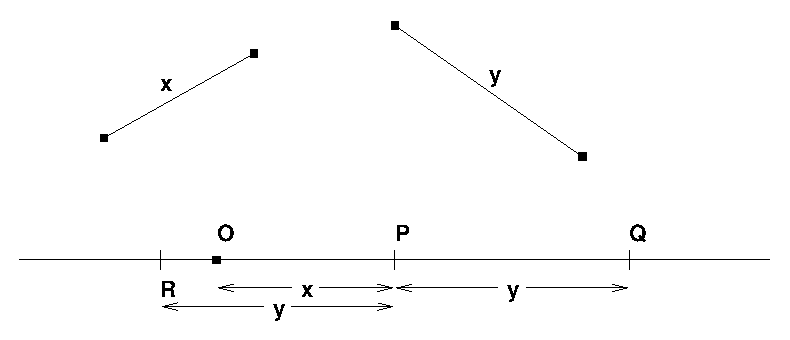
\epsfig{file=kuvat/kuvaII-2.eps}
\end{center}
%\caption{Kahden janan pituuksien summa ja erotus}
%\label{fig:summajaerotus}
\end{figure}

Kuvassa summalla ja erotuksella on geometriset vastineet janoina ja suoran pistein�:
\begin{align*}
\qquad &x+y\ \vast\ OQ\ \vast Q,  \\
\qquad &x-y\ \vast\ OR\ \vast R.
\end{align*}
Kun janan loppupiste on $O$:sta vasemmalle (suuntahan oli m��ritelty!), voidaan $OR$ tulkita 
negatiiviseksi luvuksi $x-y$. N�in on siis lukuj�rjestelm�ss� m��ritelty sek� yhteenlasku ett�
v�hennyslasku. Kun s��nt�j� $+,-$ sovelletaan per�kk�in l�htien luvusta 1 (= mittajana
sijoitettuna suoralle) n�hd��n, ett� mink� tahansa kokonaisluvun $m\in{\Z}$ geometrinen vastine
saadaan ��rellisell� m��r�ll� geometrisia operaatioita. Siis {\Z} on konstruoitu geometrisesti.
My�s mill� tahansa kokonaisluvulla jakaminen onnistuu 'viipaloimalla' luku yhdensuuntaisilla 
suorilla, joita voidaan \pain{tasossa} tuottaa harpilla ja viivoittimella (ks.\ kuvio alla).
\begin{figure}[htb]
\begin{center}
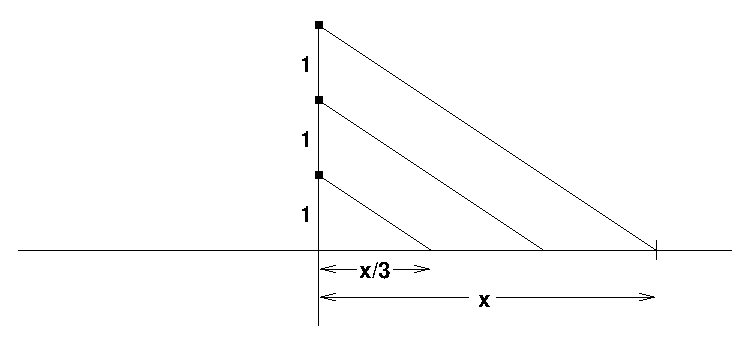
\epsfig{file=kuvat/kuvaII-3.eps}
\end{center}
\end{figure}

\pagebreak

Yleisemmin jos l�ht�kohtana on kaksi mittalukua $x,y$, niin niiden v�linen kerto- ja jakolasku
voidaan suoraan geometrisoida yhdenmuotoisten kolmioiden avulla k�ytt�en suhteita 
\begin{align*}
&\frac{z}{x}\ =\ \frac{y}{1} \quad (z=xy), \\
&\frac{z}{1}\ =\ \frac{x}{y} \quad (z=x/y).
\end{align*}
Kuvassa (alla) on
\begin{alignat*}{3}
OA &\ \vast\ 1,\quad & OB &\ \vast\ y,\quad & BC&\ \vast\ OD\ \vast\ x, \\
OE &\ \vast\ x\cdot y,\quad & AF &\ \vast\ x/y. &&
\end{alignat*} 
\begin{figure}[H]
\setlength{\unitlength}{0.67cm}
\begin{center}
\begin{picture}(12,9)(-3.5,-6)
\put(-2,0){\line(1,0){11}}
\put(-0.1,-0.1){$\bullet$} \put(-0.5,0.5){$O$}
\put(2.9,-0.1){$\bullet$} \put(3,-0.6){$A$}
\put(4.9,-0.1){$\bullet$} \put(4.9,-0.6){$B$}
\put(7.9,1.9){$\bullet$} \put(7.9,2.4){$C$}
\put(4.7,1.1){$\bullet$} \put(4.3,1.4){$F$}
\put(-1.84,-3.26){$\bullet$} \put(-1.5,-3.4){$D$}
\put(-3.02,-5.4){$\bullet$} \put(-2.6,-5.5){$E$}
\put(-3,-4){\line(3,2){11}}
\put(-3.5,-5.67){\line(3,2){12.5}}
\put(-2,-0.5){\line(4,1){11}}
\path(0,0)(-3.5,-6.34)
\put(0,-0.2){$\underbrace{\hspace{2cm}}_1$}
\put(0,0.4){$\overbrace{\hspace{3.33cm}}^y$}
\put(6.8,0.8){$x$}
\put(7.2,1.1){\vector(3,2){1.15}}
\put(6.55,0.7){\vector(-3,-2){1}}
\put(-1.3,-1.6){$x$}
\put(-1.1,-1.3){\line(10,18){0.6}}
\put(-0.5,-0.25){\vector(2,3){0.13}}
\put(-1.3,-1.8){\line(-10,-19){0.6}}
\put(-1.9,-2.92){\vector(-2,-3){0.05}}
\end{picture}
\end{center}
\end{figure}
Jatkossa nimet��n luvut, jotka ovat konstruoitavissa (janan pituutena) ��rellisell� m��r�ll�
geometrisia operaatioita, \kor{geometrisiksi luvuiksi}\footnote[2]{Englanninkielinen termi on 
'constructible numbers'. Suomennos ei ole vakiintunut.}, ja k�ytet��n t�lle lukujoukolle 
symbolia $\G$\,:
\begin{align*}
\G \ = \ \text{\{geometriset luvut\}}. 
\end{align*}
Tiedet��n jo, ett� $\G$ sis�lt�� kaikki rationaaliluvut: $\G\supset\Q$. Lis�ksi tiedet��n, ett�
$\G$ on peruslaskutoimitusten suhteen suljettu:
\[
x,y \in \G \qimpl x+y,\ x-y,\ xy,\ x/y \in \G \quad (y\neq0).
\]
T�m� merkitsee, ett� $(\G,+,\cdot)$ on \pain{kunta}.

Lukujoukon $\G$ muodostamisessa eiv�t geometrian mahdollisuudet lopu aivan 
peruslaskutoimituksiin, sill� Pythagoraan lauseen mukaan my�s operaatiot
\begin{align*}
&x,y\ \map\ \sqrt{x^{2}+y^{2}}, \quad x,y \in \G, \\
&x,y\ \map\ \sqrt{x^{2}-y^{2}}, \quad x,y \in \G,\ x \ge y
\end{align*}
ovat geometrisesti toteutettavissa. Erityisesti on siis vuosituhansia p��nvaivaa aiheuttanut
luku $\sqrt{2}$ geometristen lukujen joukossa:
\begin{figure}[H]
\setlength{\unitlength}{1cm}
\begin{center}
\begin{picture}(2.5,2.5)(-0.5,0)
\path(0,2)(0,0)(2,0)(0,2)
\put(0.8,-0.5){$1$} \put(-0.3,0.9){$1$} \put(0.9,1.1){$\sqrt{2}$}
\path(0.15,0)(0.15,0.15)(0,0.15)
\end{picture}
\end{center}
\end{figure}
Itse asiassa neli�juurioperaatio $\,x\ \map\ \sqrt{x}\,$ on geometrisesti mahdollinen, olipa
mittaluku $x \in \G$ (ajatellaan $x \geq 0$) mik� tahansa:
\begin{figure}[H]
\setlength{\unitlength}{1cm}
\begin{center}
\begin{picture}(7,4.5)(0,-0.5)
\path(3,4)(0,0)(3,0)(3,4)(8.33,0)(3,0)
%\put(3,0){\arc{0.6}{-3.14}{-1.6} \linethickness{0.05cm} \put(-0.12,0.12){\picsquare}}
%\put(3,4){\arc{0.6}{0.8}{2.2} \linethickness{0.1cm} \put(0,-0.15){\picsquare}}
\path(2.85,0)(2.85,0.15)(3,0.15) %\path(2.82,3.76)(3,3.625)(3.18,3.865)
\path(2.91,3.88)(3,3.812)(3.09,3.932)
\put(0,-0.2){$\underbrace{\hspace{3cm}}_{1}$} \put(3,-0.2){$\underbrace{\hspace{5.33cm}}_{x}$}
\put(2.8,1.9){$\left. \begin{array}{c} \vspace{3.4cm} \end{array} \right\} 
                                                                    \scriptstyle{y=\sqrt{x}}$}
\end{picture}
\end{center}
\end{figure}
T�h�n geometrian mahdollisuudet kuitenkin loppuvat, joten $\G$ koostuu kaikkiaan luvuista, jotka
on saatu mittaluvusta $1$ l�htien ��rellisell� m��r�ll� viitt� eri operaatiota: 
$+$, $-$, $\cdot\,$, $/$ ja $\sqrt{ }\,$. Kun $\G$ viel� varustetaan geometrisella 
j�rjestysrelaatiolla (janojen pituuksien vertailu harpin avulla), niin tuloksena on pelk�st��n
geometrisiin operaatioihin perustuva j�rjestetty kunta $(\G,+,\cdot,<)$. T�m� on 
rationaalilukujen kunnan pienin mahdollinen laajennus, joka t�ytt�� ehdon 
$x\in\G\,\ja\,x>0\ \impl\ \sqrt{x}\in\G$ (vrt.\ lukujoukon $\J$ konstruktio Luvussa
\ref{kunta}). On osoitettavissa, ett� kaikki geometriset luvut ovat algebrallisia (!), joten
p�tee
\[ 
\Q\ \subset\ \G\ \subset\ \A\ \subset\ \R.
\]
Kun geometriset luvut sijoitetaan em.\ tavalla kiinte�lle suoralle, voidaan n�iden lukujen 
'v�liin' ajatella sijoitelluksi my�s muut reaaliluvut. N�in ajatellen jokainen reaaliluku saa 
geometrisen vastineen
\index{lukusuora}
\kor{lukusuoran} pisteen�.

\begin{figure}[H]
\setlength{\unitlength}{1cm}
\begin{center}
\begin{picture}(14,2)(-2,0)
\put(-1,0){\line(1,0){13}}
\put(0,0){\line(0,1){0.2}}
\put(5,0){\line(0,1){0.2}}
\put(10,0){\line(0,1){0.2}}
\put(20,0){\line(0,1){0.1}}
\put(2.07,0){\line(0,1){0.1}}
\put(8.6,0){\line(0,1){0.1}}
\put(10.7,0){\line(0,1){0.1}}
\put(2.07,1){\vector(0,-1){0.6}} \put(8.6,1){\vector(0,-1){0.6}}
\put(10.7,1){\vector(0,-1){0.6}}
\put(-0.1,-0.5){$1$} \put(4.9,-0.5){$2$} \put(9.9,-0.5){$3$}
\put(1.8,1.5){$\sqrt{2}$} \put(8.5,1.5){$e$} \put(10.6,1.5){$\pi$} 
%\multiput(0,2)(0,10){2}{\line(-1,0){0.1}}
%\multiput(0,6.5)(0,1){2}{\line(-1,0){0.1}}
%\put(-0.6,8){\vector(1,-1){0.5}}
%\put(-0.6,6){\vector(1,1){0.5}}
\end{picture}
\end{center}
\end{figure}

\subsection*{Kulman mittaluku}
\index{kulma!b@kulman mittaluku|vahv}%

Kulmien k�sittelyss� geometrian mahdollisuudet ovat melko rajalliset. Kulmien yhteen- ja
v�hennyslasku onnistuu geometrisesti, kuten todettiin, ja kulman voi helposti my�s 
puolittaa eli jakaa kahteen yht� suureen osaan geometrian keinoin. Sen sijaan jo kulman
jako kolmeen yht� suureen osaan (��rellisell�) geometrisella konstruktiolla on mahdotonta,
ellei kyse ole erikoisesta (kuten suorasta) kulmasta. Geometrian keinot loppuvat my�s, kun
kulmalle yritet��n m��ritt�� sen suuruutta kuvaava mittaluku. Geometrisesti pystyt��n 
konstruoimaan vain lukujono, jonka raja-arvo mittaluku on, eli mittaluku saadaan selville
vain p��ttym�tt�m�ll� konstruktiolla. 
\begin{multicols}{2} \raggedcolumns
Tarkastellaan kulmaa $\kulma AOB$, miss� pisteet $A$ ja $B$ on sijoitettu $O$-keskisen
\index{yksikk�ympyr�}%
\kor{yksikk�ympyr�n} keh�lle, ts.\ janat $OA$ ja $OB$ ovat valitun mittajanan pituiset
(vastaten lukua $1$ lukusuoralla).
\begin{figure}[H]
\setlength{\unitlength}{1cm}
\begin{center}
\begin{picture}(4.5,3.5)(-0.5,0.3)
\put(2,2){\bigcircle{4}}
\put(2,2){\line(3,1){1.9}}
\put(2,2){\line(1,3){0.63}}
\put(1.9,1.5){$O$} \put(4,2.55){$A$} \put(2.55,4){$B$}
\end{picture}
\end{center}
\end{figure}
\end{multicols}
Kuvion tilanteessa asetetaan kulman $\kulma AOB$ mittaluvuksi yksikk�ympyr�n
\kor{kaarenpituus} pisteiden $A$ ja $B$ v�lill�. Koska vaihtoehtoja on kaksi, on
p��tett�v�, mitataanko sis�- vai ulkokulmaa. Seuraavaksi on ratkaistava vakavampi ongelma:
Miten m��ritell� ympyr�kaaren pituus? Seuraavassa ongelman ratkaisussa yhdistell��n
geometrian ja algebran keinoja.

Koska kulman $\kulma OAB$ puolitus onnistuu geometrisesti, niin saman tien kulma on
jaettavissa $n=2^k$ yht� suureen osaan jokaisella $k\in\N$. Olkoon $k\in\N$ annettu
ja merkit��n jaossa syntyvi� osakulmia $\kulma P_{i-1} O P_i,\ i=1 \ldots n=2^k$,
miss� $P_0=A$, $P_n=B$ ja muutkin pisteet $P_i$ ovat samalla $O$-keskisell�
ympyr�kaarella. Yhdistet��n nyt per�kk�iset pisteet $P_i$ janoilla \kor{murtoviivaksi}
$P_0 \ldots P_n$ ja asetetaan $\,a_k=$ ko.\ murtoviivan pituus, ts.\ $\,a_k=$ janojen 
$P_{i-1}P_i,\ i=1 \ldots n\,$ pituuksien summa. On ilmeist�, ett� lukujonon $\seq{a_k}$
jokainen termi on m��r�tt�viss� geometrisesti l�htien  luvusta $a_0=$ janan $AB$ pituus,
jolloin on $a_k/a_0\in\G\ \forall k$ (mahdollisesti $a_0\not\in\G$). Kuviossa on
konstruoitu murtoviiva $P_0 \ldots P_n$ indekseill� $k=0,1,2$, kun mitattavana on
suora kulma.
\begin{figure}[H]
\setlength{\unitlength}{1cm}
\begin{picture}(6,4.5)(-0.3,-0.5)
\put(0,0){\line(1,0){4}}
\put(0,0){\line(0,1){4}}
\put(0,0){\arc{6}{-1.57}{0}}
\path(3,0)(0,3)
\put(3.1,0.15){$P_0$} \put(0.1,3.15){$P_1$}
\put(1,-0.8){$k=0$}
\put(5,0){\line(1,0){4}}
\put(5,0){\line(0,1){4}}
\put(5,0){\arc{6}{-1.57}{0}}
\path(8,0)(7.121,2.121)(5,3)
\path(5,0)(7.121,2.121)
\put(8.1,0.15){$P_0$} \put(5.1,3.15){$P_2$} \put(7.22,2.27){$P_1$}
\put(6,-0.8){$k=1$}
\put(10,0){\line(1,0){4}}
\put(10,0){\line(0,1){4}}
\put(10,0){\arc{6}{-1.57}{0}}
\path(13,0)(12.772,1.148)(12.121,2.121)(11.148,2.772)(10,3)
\path(10,0)(12.772,1.148) \path(10,0)(12.121,2.121) \path(10,0)(11.148,2.772)
\put(13.1,0.15){$P_0$} \put(10.1,3.15){$P_4$} \put(12.22,2.27){$P_2$}
\put(12.87,1.3){$P_1$} \put(11.25,2.92){$P_3$}
\put(11,-0.8){$k=2$}
%\dashline{0.2}(0.3,3.4)(3.3,1.4)
%\put(1.56,2.8){$P$}
%\path(2.93,0.6)(3.3,0.6)
%\path(2.08,3.1)(2.8,3.1)
\end{picture}
\end{figure}
Pythagoraan lauseeseen vedoten on helppo n�ytt��, ett� lukujono $\seq{a_k}$ on aidosti
kasvava (Harj.teht.\,\ref{H-II-1: suoran kulman mitta}a), ja geometrisin perustein on my�s
osoitettavissa, ett� $\seq{a_k}$ on rajoitettu lukujono 
(Harj.teht.\,\ref{H-II-1: suoran kulman mitta}b). T�m�n j�lkeen on turvattava algebraan: 
Koska $\seq{a_k}$ siis on kasvava ja rajoitettu lukujono, niin on olemassa raja-arvo 
$\lim_k a_k=a\in\R$ (Lause \ref{monotoninen ja rajoitettu jono}, 
M��ritelm� \ref{reaaliluvut desimaalilukuina}). M��ritell��n kaaren $AB$ pituus, eli kulman 
$\kulma AOB$ mittaluku, kyseisen� raja-arvona $a$. 

Mittayksikk�� kulman kaarenpituusmittauksessa sanotaan \kor{radiaaniksi}. Tunnetusti
luku $\,\pi=3.14159..\,$ m��ritell��n yksikk�ympyr�n puolikkaan kaarenpituutena, eli
\[
\boxed{\kehys\quad \pi \,=\, \text{oikokulman mittaluku}. \quad}
\]
Koska $\pi$ on transkendenttinen luku (ks.\ Luku \ref{reaalilukujen ominaisuuksia}), niin
my�s suoran kulman mittaluku ($=\pi/2$) on transkendenttinen, samoin esimerkiksi
tasasivuisen kolmion kulman mittaluku ($=\pi/3$).

Kulmia on perinteisesti mitattu my�s \kor{asteina} ($\aste$), jolloin oikokulman mitaksi
on sovittu $180\aste$. Yleisemmin mittaluvut asteina ja radiaaneina saadaan skaalaamalla
toisistaan:
\[
\boxed{\kehys\quad \text{kulma asteina}\ 
               =\ \frac{180}{\pi}\,\cdot\,\text{(kulma radiaaneina)}. \quad}
\]

\Harj
\begin{enumerate}

\item \label{H-II-1: kulmat}
a) Suoran leikatessa kaksi yhdensuuntaista suoraa syntyy kahdeksan kulmaa. N�yt�, ett�
n�ist� jokainen on yht� suuri kolmen muun kanssa. \newline
b) Todista: Kolmion kulmien summa = oikokulma.

\item \label{H-II-1: yhdenmuotoisuus} \index{keskijana (kolmion)}
a) Jana jakaa suorakulmaisen kolmion kahteen osaan siten, ett� syntyy kolme yhdenmuotoista 
kolmiota. L�htien t�st� ajatuksesta ja kolmioiden yhdenmuotoisuusopista todista Pythagoraan 
lause! \newline
b) Kolmion \kor{keskijana} yhdist�� kolmion k�rjen vastakkaisen sivun keskipisteeseen.
L�htien kolmioiden yhdenmuotoisuusopista todista: Kolmion $ABC$ keskijana $AD$ puolittaa
jokaisen janan $BC$ suuntaisen janan, jonka p��tepisteet ovat sivuilla $AB$ ja $AC$.

\item \index{kultainen leikkaus}
Esit� geometrinen konstruktio (aseina harppi ja viivoitin), jonka tulos on \newline
a) \ ympyr�, joka kulkee annetun kolmen pisteen kautta, \newline
b) \ annetun kolmion sis��n piirretty (suurin mahdollinen) ympyr�, \newline
c) \ suora, joka kulkee annetun pisteen kautta ja sivuaa annettua ympyr��,
d) \ annetun janan $AB$ \kor{kultainen leikkaus} eli janalla oleva piste $C$ siten, ett�
jos $a,b,c$ ovat janojen $AB$, $AC$ ja $CB$ pituudet, niin $\,a/b=b/c$.

\item
Seuraavista luvuista kaksi ei ole geometrisia. Mitk� kolme ovat\,? \vspace{1mm}\newline
a) \ $\sqrt[1024]{17}$ $\quad$ b) \ $\sqrt[3]{512}$ $\quad$ c) \ $\sqrt[6]{343}$ $\quad$
d) \ $\sqrt[3]{7\sqrt{2}+5}$ $\quad$ e) \ $\sqrt[3]{5\sqrt{2}+7}$

\item (*) \label{H-II-1: suoran kulman mitta}
Suoran kulman mittaluku radiaaneina m��ritell��n raja-arvona $\,a=\lim_k a_k$, miss� $4a_k=$ sen 
s��nn�llisen $2^{k+2}$-kulmion piiri, jonka k�rjet ovat yksikk�ympyr�ll�. \vspace{1mm}\newline
a) N�yt�, ett� lukujono $\seq{a_k}_{k=0}^\infty$ on aidosti kasvava. \newline
b) N�yt�, ett� $a_k < 2\ \forall k$. \newline
c) N�yt�, ett� $\seq{a_k}$ on laskettavissa palautuvana lukujonona
\[
a_0=\sqrt{2}, \quad 
a_{k+1}=\frac{2a_k}{\sqrt{2+\sqrt{4-(2^{-k}a_k)^2}}}\,, \quad k=0,1,\ldots
\]
Laske $a_k,\ k=1 \ldots 5$ ja vertaa lukuun $\tfrac{\pi}{2}$.

\end{enumerate}
\section{Tason vektorit} \label{tasonvektorit}
\alku
\index{vektoria@vektori (geometrinen)!a@tason \Ekaksi|vahv}%

\kor{Vektori} on matemaattisena käsitteenä hieman kaksijakoinen. Se voi olla lähtökohtaisesti 
geometrinen olio, jolloin se sovelluksissa ajatellaan usein fysikaalisena, 'maailmassa 
vaikuttavana'. Tällaisia 'fysiikkavektoreita' ovat mm.
\begin{itemize}
\item  paikka, nopeus, kiihtyvyys, kulmanopeus
\item  voima, momentti
\item  X-kentän voimakkuus, X=gravitaatio, sähkö, magneetti...
\end{itemize}
Toisaalta vektori voidaan tulkita myös algebrallisesti, jolloin päädytään geometris-fysikaalista
vektoria yleisempään (myös abstraktimpaan) vektorikäsitteeseen. Jäljempänä nähdään ensimmäisiä
esimerkkejä myös tällaisista 'matematiikkavektoreista' (myöhemmin esimerkkejä tulee paljon 
lisää). Jatkossa lähtökohta vektorin käsitteeseen on kuitenkin aluksi geometrinen.

Euklidisessa tasossa \Ekaksi\, vektori määritellään geometrisesti \kor{suuntajanana}, ts. 
janana, jolla on suunta. Ajatus on tällöin, että jana sisältyy sen toisesta päätepisteestä 
lähtevään puolisuoraan. Puolisuoran ilmaisema suunta kuvataan janan päähän merkityllä
nuolenkärjellä:
\begin{figure}[H]
\setlength{\unitlength}{1cm}
\begin{center}
\begin{picture}(13,6)(0,-0.5)
%\Thicklines
\put(1,3){\line(2,1){5}} \put(0,0){\line(4,1){4}}
\put(9,3){\vector(2,1){3}} \put(12,1){\vector(-4,-1){3}}
\put(0.95,3.1){\line(1,-2){0.1}} \put(0.9,2.5){$A$}
\put(3.95,4.6){\line(1,-2){0.1}} \put(3.9,4.0){$B$}
\put(3.975,1.1){\line(1,-4){0.05}} \put(3.925,0.5){$A$}
\put(0.975,0.35){\line(1,-4){0.05}} \put(0.925,-0.25){$B$}
\put(8.9,2.5){$A$} \put(11.9,4){$B$}\put(11.925,0.5){$A$} \put(8.925,-0.25){$B$}
\put(6.5,4){$\hookrightarrow$}
\put(6.5,0){$\hookrightarrow$}
\end{picture}
\end{center}
\end{figure}
Vektorilla tarkoitetaan täsmällisemmin vain suuntajanan sisältävää \pain{osatietoa} 
\[
\{\text{(janan) pituus, suunta}\}.
\] 
Tiettyyn suuntajanaan liittyvä vektori merkitään $\overrightarrow{AB}$, yleisemmin 
käytetään vektorimerkintöjä $\vec a, \vec b, \vec v$ jne.

Huomattakoon, että vektori $\overrightarrow{AB}$ siis \pain{ei} 'tiedä', missä piste
$A$ sijaitsee euklidisessa tasossa. Näin ollen 'vektoria saa siirtää', kunhan 'ei kierrä
eikä venytä'. (Fysikaalinen vastine: Voiman vaikutus on sama vaikutuspisteestä
riippumatta.) 

Jos tunnetaan vektorit $\vec a=\overrightarrow{AB}$ ja $\vec b=\overrightarrow{BC}$,
niin tunnetaan myös $\vec c=\overrightarrow{AC}$\,:
\begin{figure}[H]
\setlength{\unitlength}{1cm}
\begin{center}
\begin{picture}(6,5)
%\Thicklines
\put(0,0){\vector(2,3){2}} \put(2,3){\vector(4,1){4}} \put(0,0){\vector(3,2){6}}
\put(-0.1,-0.1){$\bullet$} \put(1.9,2.9){$\bullet$} \put(5.9,3.9){$\bullet$}
\put(-0.2,0.3){$A$} \put(1.9,3.2){$B$} \put(5.9,4.2){$C$}
\put(0.9,1.8){$\vec a$} \put(4.8,3.8){$\vec b$} \put(4,2.8){$\vec c$}
\end{picture}
\end{center}
\end{figure}
\index{laskuoperaatiot!c@tason vektoreiden|(}%
Sanotaan, että $\vec c$ on vektoreiden $\vec a, \vec b$ \kor{summavektori} ja merkitään
\[
\vec c=\vec a+\vec b.
\]
Summa määrätään siis geometrisesti kolmiodiagrammilla. Näin määritellylle vektorien 
yhteenlaskulle pätevät tavanomaiset vaihdanta- ja liitäntälait:
\begin{itemize}
\item[(V1)] $\quad \vec a+\vec b = \vec b+\vec a$
\item[(V2)] $\quad (\vec a+\vec b\,)+\vec c = \vec a+(\vec b+\vec c\,)$
\end{itemize}
Tässä ei ole kyse aksioomista (vrt.\ vastaavat kunta-aksioomat, Luku \ref{kunta}) vaan
väittämistä, joiden todistus on geometrinen:
\begin{figure}[H]
\setlength{\unitlength}{1cm}
\begin{center}
\begin{picture}(14,5)
%\Thicklines
\put(0,0){\vector(2,3){2}} \put(2,3){\vector(4,1){4}}
\dashline{0.2}(0,0)(4,1) \dashline{0.2}(4,1)(6,4)
\put(3.9,0.975){\vector(4,1){0.1}} \put(5.9,3.85){\vector(2,3){0.1}}
\put(1.2,2.2){$\vec a$} \put(5.2,4){$\vec b$} \put(3.5,1.1){$\vec b$} \put(5.8,3.3){$\vec a$}

\put(6,0){\vector(2,3){2}} \put(8,3){\vector(4,1){4}}
\dashline{0.2}(6,0)(12,4) \put(11.9,3.933){\vector(3,2){0.1}} \put(12,4){\vector(1,-1){2}}
\put(6,0){\vector(4,1){8}}
\dashline{0.2}(8,3)(14,2) \put(13.9,2.0167){\vector(4,-1){0.1}}
\put(7.2,2.2){$\vec a$} \put(11.2,4){$\vec b$} \put(13.6,2.5){$\vec c$} 
\put(12,1.1){$\vec a+\vec b+\vec c$}
\put(12.9,2.3){$\scriptstyle{\vec b+\vec c}$} \put(11.5,3.3){$\scriptstyle{\vec a+\vec b}$}
\end{picture}
\end{center}
\end{figure}
Vektorin $\vec a = \overrightarrow{AB}$
\index{itseisarvo}%
\kor{itseisarvo} (arkisemmin 'pituus') on
\[
\abs{\vec a}=|\overrightarrow{AB}|=\abs{AB}=\text{janan }AB\text{ pituus}.
\]
Tälle pätee \kor{kolmioepäyhtälö} (vrt.\ Lause \ref{kolmioepäyhtälö})
\index{kolmioepäyhtälö!b@tason vektoreiden}%
\[
\abs{\vec a+\vec b} \le \abs{\vec a}+\abs{\vec b}.
\]
Jos $\lambda \in \R$, niin $\lambda \vec a$ tarkoittaa
\index{skaalaus (vektorin)}%
\kor{skaalattua} vektoria, jolle pätee:
\begin{itemize}
\item[(1)] $\quad |\lambda \vec a|=|\lambda||\vec a|$
\item[(2)] $\quad \lambda \vec a \uparrow\uparrow \vec a,
                                 \text{ jos } \lambda > 0, \text{ ja }
                  \lambda \vec a \uparrow\downarrow \vec a, \text{ jos } \lambda<0$
\end{itemize}
Tässä $\uparrow\uparrow$ tarkoittaa yhdensuuntaisuutta ja $\uparrow\downarrow$ 
vastakkaissuuntaisuutta. Vektorin skaalausta $\vec a \map \lambda \vec a \ (\lambda \in \R)$
sanotaan vektorialgebrassa yleisemmin \kor{skalaarilla kertomiseksi}. Skaalaajia eli
reaalilukuja kutsutaan siis tässä laskuoperaatiossa
\index{skalaari}%
\kor{skalaareiksi}. Skalaarilla kertomisen ja yhteenlaskun
määritelmistä on pääteltävissä (Harj.teht.\,\ref{H-II-1: perusteluja}a), että seuraavat
'luonnonmukaiset' säännöt ovat voimassa (vrt.\ kunta-aksioomat Luvussa \ref{kunta})\,:
\begin{itemize}
\item[(V3)] $\quad (\lambda + \mu)\vec a = \lambda \vec a + \mu \vec a$
\item[(V4)] $\quad \lambda(\mu \vec a\,) = (\lambda \mu)\vec a$
\item[(V5)] $\quad \lambda(\vec a + \vec b\,)= \lambda \vec a + \lambda \vec b$
\item[(V6)] $\quad 1 \vec a =  \vec a$
\end{itemize}
Operaation $\vec a \kohti \lambda \vec a$ määritelmän mukaisesti on $|0 \vec a|=0$.
Tällaista vektoria sanotaan
\index{nollavektori}%
\kor{nollavektoriksi} ja merkitään $\,0 \vec a = \vec 0$.
Nollavektorin suunta on epämääräinen  (ei määritelty). Nollavektori on vektorien
yhteenlaskun nolla-alkio, ts.\ pätee
\begin{itemize}
\item[(V7)] $\quad \vec a + \vec 0 = \vec a\ \forall \vec a$ 
\end{itemize}
Jokaisella vektorilla $\vec a$ on myös
\index{vastavektori}%
\kor{vastavektori} $-\vec a$, jolle pätee
\begin{itemize} 
\item[(V8)] $\quad \vec a + (-\vec a\,) = \vec 0$
\end{itemize}
Nimittäin kun säännössä (V3) valitaan $\lambda=1, \mu=-1$ ja käytetään nollavektorin
määritelmää ja sääntöä (V6), niin seuraa
\[
-\vec a = (-1)\,\vec a.
\]
Vastavektorin avulla tulee määritellyksi myös vektorien vähennyslasku:
\[
\vec a - \vec b = \vec a + (-\vec b\,).
\]
\begin{figure}[H]
\setlength{\unitlength}{1cm}
\begin{center}
\begin{picture}(6,2.3)(2,0.5)
%\Thicklines
\put(4,0){\vector(2,3){2}} \put(4,0){\vector(4,1){4}} \put(8,1){\vector(-1,1){2}}
\dashline{0.2}(4,0)(2,2) \put(2.1,1.9){\vector(-1,1){0.1}} 
\dashline{0.2}(6,3)(2,2) \put(2.1,2.025){\vector(-4,-1){0.1}}
\put(5.8,2.3){$\vec a$} \put(7.6,0.4){$\vec b$} \put(6.5,2.7){$\vec a-\vec b$} 
\put(2.7,1.4){$\vec a+(-\vec b\,)$}
\end{picture}
\end{center}
\end{figure}
Säännöt (V1)--(V8), yhdessä nollavektorin ja vastavektorin määritelmien kanssa, muodostavat
(tason vektoreiden)) \kor{vektorialgebran} laskulait.
\index{laskuoperaatiot!c@tason vektoreiden|)}
\begin{Exa} \label{kolmion keskipiste}
Laskulaeista (V1)--(V8) seuraava identiteetti
\[
\vec a + \frac{2}{3} \left( \frac{1}{2}\vec b - \vec a \right)\ 
             =\ \vec b + \frac{2}{3} \left( \frac{1}{2}\vec a - \vec b \right)\
             =\ \frac{2}{3} \left[ \vec b + \frac{1}{2}\left( \vec a - \vec b \right) \right]\
             =\ \frac{1}{3} \left( \vec a + \vec b \right)
\]
voidaan lukea: Kolmion keskijanat leikkaavat toisensa samassa pisteessä, joka jakaa keskijanat
suhteessa $2:1$ (vrt.\ kuvio). Leikkaupistettä sanotaan 
\index{keskizza@keskiö (kolmion)}%
kolmion \kor{keskiöksi} (keskipisteeksi). \loppu
\begin{figure}[H]
\setlength{\unitlength}{1cm}
\begin{center}
\begin{picture}(6.5,4.6)(0,0)
%\Thicklines
\put(0,0){\vector(1,2){2}} \put(0,0){\vector(1,0){6}}
\path(2,4)(6,0)(1,2)
\drawline(2,4)(3,0) \drawline(0,0)(4,2) \put(0,0){\vector(2,1){2.67}}
\put(1.4,3.5){$\vec a$} \put(5.5,-0.5){$\vec b$}
\put(0,-0.5){$A$} \put(1.9,4.2){$B$} \put(6.2,-0.1){$C$}
\put(1.2,1.2){$\scriptstyle{\frac{1}{3}(\vec a+\vec b\,)}$}
\end{picture}
\end{center}
\end{figure}
\end{Exa}

\subsection*{Vektoriavaruus}
\index{vektoric@vektoriavaruus|vahv}%

Jos tason vektorien joukkoa merkitään symbolilla $V$, niin edellä olevilla määritelmillä on 
syntynyt algebra, joka merkittäköön $(V,\R)$. Laskusääntöjen (V1)--(V8) (yleisemmin:
aksioomien) ollessa voimassa sanotaan, että kyseessä on (lineaarinen) \kor{vektoriavaruus}.
Käsitteeseen siis sisältyvät
\index{laskuoperaatiot!ca@ yleisen vektoriavaruuden}
\begin{itemize}
\item  vektorien muodostama joukko $V$ (jossa operoidaan)
\item  vektorien yhteenlasku (+)
\item  nk. \kor{skalaarien} muodostama \kor{kertojakunta}, tässä = $\R$
\item  skalaarin ja vektorin kertolasku
\end{itemize}
\index{skalaari} \index{kertojakunta}%
Lyhennetty sanonta '$V$ on vektoriavaruus' tarkoittaa koko tätä algebraa, jolloin 
kertojakunta on juuri $\R$, tai muuten asiayhteydestä selvä. Sanonnat \kor{reaalikertoiminen}
vektoriavaruus tai yleisemmin \kor{$\K$-kertoiminen} vektoriavaruus kiinnittävät kertojakunnan
tarkemmin. Kertojakunnan ei siis tarvitse olla $\R$, vaan se voisi olla esim. $\K=\Q$ tai 
$\K=\G=\{\text{geometriset luvut}\}$. Lineaarinen vektoriavaruus on hyvin keskeinen käsite
matematiikassa, ja sillä on keskeinen rooli myös monissa matematiikan sovelluksissa.

\subsection*{Kanta ja koordinaatisto}
\index{kanta|vahv} \index{koordinaatisto|vahv}%

Olkoon $\vec v \in V$ mielivaltainen tason vektori ja $\vec a, \vec b \in V$ kaksi vektoria, 
joille pätee
\[
\vec a, \vec b \neq \vec 0 ,\quad \vec a \neq \lambda \vec b \quad \forall \ \lambda \in \R.
\] 
Tällöin voidaan geometrisella konstruktiolla (ks.\ kuvio) löytää yksikäsitteiset $x,y \in \R$
siten, että
\[
\vec v = x \vec a + y \vec b.
\]
\begin{figure}[H]
\setlength{\unitlength}{1cm}
\begin{center}
\begin{picture}(6,4.5)(0,-0.5)
%\Thicklines
\put(0,0){\vector(1,1){4}} \put(0,0){\vector(1,0){2}} \put(0,0){\vector(3,1){6}}
\put(0,0){\vector(1,0){4}} \put(0,0){\vector(1,1){2}}
\dashline{0.2}(6,2)(2,2) \dashline{0.2}(6,2)(4,0)
\put(3.1,3.6){$\vec b$} \put(0.9,1.6){$y\vec b$} \put(1.5,-0.5){$\vec a$} 
\put(3.3,-0.5){$x\vec a$} \put(5.5,2.2){$\vec v$}
\end{picture}
\end{center}
\end{figure}
Sanotaan tällä perusteella, että $\vec v$ on $\vec a$:n ja $\vec b$:n
\index{lineaariyhdistely}%
\kor{lineaariyhdistely} (lineaarinen yhdistely, \kor{lineaarikombinaatio}) ja että
$x \vec a$ ja $y \vec b$ ovat $\vec v$:n
\index{komponentti (vektorin)}%
(vektori)\kor{komponentit} $\vec a$:n ja $\vec b$:n suuntaan. 

Kun siis kaksi em.\ ehdot täyttävää vektoria on valittu, on koko $V$ esitettävissä muodossa
\[
V=\{x \vec a + y \vec b \mid x,y \in \R\}.
\]
Sanotaan, että vektoripari $\{ \vec a, \vec b \}$ on $V$:n \kor{kanta}\footnote[2]{Kanta on
vektoreiden j\pain{är}j\pain{estett}y joukko, joten merkintä $(\vec a,\vec b)$ olisi
loogisempi. Erinäisten sekaannusten välttämiseksi käytetään tässä yhteydessä kuitenkin
yleisemmin aaltosulkeita.} ja että $x,y$ ovat vektorin $\vec v = x \vec a + y \vec b \in V$
\index{koordinaatti (vektorin)}%
\kor{koordinaatit} kannassa $\{\vec a,\vec b\,\}$. Jos koordinaatit esitetään lukuparina
$(x,y)$ (pari = kahden alkion järjestetty joukko), niin on synnytetty yhteys $V$:n ja
tällaisten lukuparien joukon välille. Merkitään jälkimmäistä joukkoa symbolilla $\Rkaksi$,
äännetään 'R kaksi':
\[
\Rkaksi = \{ (x,y) \mid x \in \R\,\ja\,y \in \R \}.\index{karteesinen tulo|av}%
\footnote[3]{Joukko $\R^2$ voidaan myös  merkitä $\R\times\R$, jolloin käytetään
joukko-opillista \kor{karteesisen tulon} merkintää
\[
A \times B = \{ (x,y) \mid x \in A\,\ja\,y \in B \}.
\] 
Tämä luetaan '$A$:n ja $B$:n karteesinen tulo', tai vain '$A$ risti $B$'. Joukon
$A \times B$ alkiot ovat siis pareja. Näiden välinen samastusrelaatio on
\[
(x_1,y_1) = (x_2,y_2) \qekv  x_1=x_2\ \wedge\ y_1=y_2.
\] }
\]

Em. sopimuksilla on itse asiassa luotu \kor{kääntäen yksikäsitteinen} (=molempiin suuntiin 
yksikäsitteinen)
\index{vastaavuus ($\ensuremath  {\leftrightarrow }$)}%
\kor{vastaavuus} $V$:n ja $\Rkaksi$:n välille. Merkitään tätä: 
\[
V \vast \Rkaksi.
\]
Vastaavuuteen liittyen nimetään $\Rkaksi$ kantaan $\{\vec a, \vec b\,\}$ liittyväksi $V$:n
\index{koordinaattiavaruus}% 
\kor{koordinaatti-avaruudeksi}. Nimitys jo viittaa siihen, että myös $\Rkaksi$ on tulkittavissa
\index{vektorib@vektori (algebrallinen)!a@$\R^2$:n}%
lineaariseksi vektoriavaruudeksi. Nimittäin kaikki vektoriavaruuden laskulait ovat voimassa,
kun yhteenlasku ja skalaarilla kertominen $\Rkaksi$:ssa määritellään
\index{laskuoperaatiot!cb@vektoriavaruuden $(\Rkaksi,\R)$}
\begin{align*}
(x_1,y_1)+(x_2,y_2)& = (x_1+x_2,y_1+y_2), \\
\lambda(x,y) &= (\lambda x, \lambda y).
\end{align*}
Nämä operaatiot myös vastaavat $V$:n laskutoimituksia, sillä
\begin{align*}
\vec v_1=x_1 \vec a + y_1 \vec b, \ \vec v_2= x_2 \vec a + y_2 \vec b \ 
                               &\impl \ \vec v_1 + \vec v_2 = (x_1+x_2)\vec a 
                                                                        + (y_1+y_2)\vec b, \\
\vec v = x \vec a +y \vec b \  &\impl \ \lambda \vec v = (\lambda x)\vec a +(\lambda y)\vec b.
\end{align*}

Vektoriavaruus $(\Rkaksi,\R)$, mainituin laskuoperaatioin, on esimerkki (lajissaan ensimmäinen)
algebrallisten vektoreiden muodostamasta vektoriavaruudesta. Tämä avaruus on
siis geometrisista tulkinnoista vapaa. Toisaalta tulkitsemalla $(\Rkaksi,\R)$ tason vektorien
koordinaattiavaruudeksi (valitussa kannassa) saadaan vektorien laskuoperaatiot muunnetuksi 
algebralliseen muotoon. Esimerkiksi yhteenlaskussa tällainen laskukaavio on
\[
\begin{array}{cccccc}
&\vec v_1   &  &\vec v_2   &     &\vec v_1+\vec v_2 \\
&\downarrow &  &\downarrow &     &\uparrow \\ 
&(x_1,y_1)  &  &(x_2,y_2)  &\map &(x_1+x_2,y_1+y_2)
\end{array}
\]
Kaavion etuna on, että itse laskuoperaatiossa ei tarvita mitään tietoa vektorien 'ulkonäöstä'.
Monia geometrian tuloksia voidaan tällä tavoin johtaa algebran keinoin (vrt.\ Esimerkki 
\ref{kolmion keskipiste} edellä).

Koordinaattiavaruus $\Rkaksi$ voidaan yhtä hyvin liittää myös siihen alkuperäiseen 
pisteavaruuteen $\Ekaksi$, josta koko vektoriajatus oli lähtöisin. Nimittäin jos vektoreita 
ajatellaan $\Ekaksi$:n suuntajanoina, 'joita voi siirrellä', niin voidaan yhtä hyvin ajatella,
että jokainen vektori vastaa yksikäsitteistä suuntajanaa, jonka lähtöpiste on kiinteä piste $O$.
Näin on synnytetty $\Ekaksi$:n ja $V$:n kääntäen yksikäsitteinen vastaavuus:
\[
P \in \Ekaksi \ \leftrightarrow \ \overrightarrow{OP} \in V.
\]
Kun nyt tulkitaan myös edellä valitut kantavektorit $\vec a, \vec b$ pisteestä $O$ alkaviksi
suuntajanoiksi, niin euklidiseen tasoon on luotu \kor{koordinaatisto}\footnote[2]{Ajatuksen 
koordinaatiston avulla tapahtuvasta geometrian aritmetisoimisesta toi matematiikkaan 
ranskalainen filosofi-matemaatikko \hist{Ren\'e Descartes} (1596-1650) tutkielmassaan 
''La g\'eom\'etrie'', joka ilmestyi laajemman filosofisen teoksen liitteenä vuonna 1637. 
Tutkielma merkitsi \kor{analyyttisen geometrian} alkua, ja enteili yleisemminkin geometrian 
'algebralisoitumista' --- trendiä, joka erityisesti tietokoneiden aikakaudella on entisestään
vahvistunut. \index{Descartes, R.|av}}, jota merkitään $\{O,\vec a,\vec b\}$. Pistettä $O$
sanotaan koordinaatiston 
\index{origo}%
\kor{origoksi}.

\begin{figure}[H]
\setlength{\unitlength}{1cm}
\begin{center}
\begin{picture}(6,4)(-2,-0.2)
%\Thicklines
\put(0,0){\vector(3,2){4}} \put(0,0){\vector(-2,3){2}}
\put(-0.1,-0.5){$O$} \put(-1.7,2.8){$\vec a$} \put(3.5,2.6){$\vec b$}
\end{picture}
\end{center}
\end{figure}
\index{koordinaatti (pisteen)}%
Jos $P \in \Ekaksi$ ja $\Vect{OP} = x \vec a + y \vec b$, niin sanotaan, että \kor{pisteen}
$P$ \kor{koordinaatit} valitussa koordinaatistossa $\{O,\vec a,\vec b\,\}$ ovat 
$(x,y)$. Koordinaatiston ollessa kiinitetty voidaan koordinaattiparia $(x,y)$ haluttaessa 
pitää $P$:n 'nimenä', jolloin on lupa kirjoittaa muitta mutkitta
\[
P=(x,y).
\]
Näin on luotu kääntäen yksikäsitteinen vastaavuus $\Ekaksi \ \leftrightarrow \ \Rkaksi$.
\begin{Exa} Olkoon $T$ tason (aito) kolmio, jonka kärkikipisteet ovat $0,A,B$. Merkitään 
$\vec a=\Vect{OA}$, $\vec b=\Vect{OB}$. Tällöin $T$:n kärkipisteet, $T$:n sivujen 
keskipisteet ja $T$:n keskiö koordinaattistossa $\{O,\vec a,\vec b\,\}$ ovat
(vrt.\ Esimerkki \ref{kolmion keskipiste})
\begin{align*}
&\text{kärkipisteet:} \quad O=(0,0), \quad A=(1,0), \quad B=(0,1), \\
&\text{sivujen keskipisteet:} \quad O'=(1/2,1/2), \quad A'=(0,1/2), \quad B'=(1/2,0), \\
&\text{keskiö:} \quad C=(1/3,1/3). \quad\loppu
\end{align*}
\end{Exa}
Koordinaatistoon tarvitaan siis ensinnäkin referenssipiste $O$. Tästä nk. origosta valitaan
kaksi suuntaa, jotka määrääväät vektoreiden $\vec a, \vec b$ suunnat. Vielä päätetään, että 
mitattaessa etäisyyttä $O$:sta on pituusyksikkö $\alpha$ mentäessä $\vec a$:n suuntaan ja 
$\beta$ mentäessä $\vec b$:n suuntaan. Tässä $\alpha,\beta \in \R$ ja $\alpha,\beta>0$. Kun nyt
valitaan $\vec a$ ja $\vec b$ siten, että $|\vec a|=\alpha$ ja $|\vec b|=\beta$, ovat $\vec a$
ja $\vec b$ yksikäsitteisesti määrätyt ja koordinaatisto siis valmis. Origon kautta kulkevia
suoria
\begin{align*}
S_1=\{ P \in \Ekaksi \ | \ \overrightarrow{OP} = \lambda \vec a, \ \lambda \in \R \}, \\
S_2=\{ P \in \Ekaksi \ | \ \overrightarrow{OP} = \mu \vec b, \ \mu \in \R \},
\end{align*}
\index{suuntavektori} \index{koordinaattiakseli}%
joiden \kor{suuntavektoreina} ovat $\vec a, \vec b$, sanotaan \kor{koordinaattiakseleiksi}.
\begin{figure}[H]
\setlength{\unitlength}{1cm}
\begin{center}
\begin{picture}(10,6)(-3,-2)
\Thicklines
\put(0,0){\vector(3,2){4}} \put(0,0){\vector(-1,1){2}}
\thinlines
\put(0.3,-0.1){$O=(0,0)$} \put(-2.1,1.4){$\vec a$} \put(3.5,2.7){$\vec b$}
\put(-3,-2){\line(3,2){8}} \put(2,-2){\line(-1,1){5}}
\put(-1.8,2){$(1,0)$} \put(4,2.2){$(0,1)$}
\put(2.2,-2){$S_1$} \put(-2.5,-2){$S_2$}
\put(-0.07,-0.07){\piste} \put(3.93,2.6){\piste} \put(-2.07,1.93){\piste}
\end{picture}
\end{center}
\end{figure}

\subsection*{Lineaarinen riippumattomuus}
\index{lineaarinen riippumattomuus|vahv}

Koordinaatiston kantavektoreista $\vec a,\vec b$ edellä tehdyt oletukset
($\vec a,\vec b \neq \vec 0$ ja $\vec a,\vec b$ eivät saman- tai vastakkaissuuntaiset) 
voidaan asettaa lyhyemmin ehtona
\begin{equation} \label{lin riippumattomat}
x \vec a + y \vec b = \vec 0 \qimpl x=y=0. \tag{$\star$}
\end{equation}
Jos tason vektoreilla on ominaisuus \eqref{lin riippumattomat}, niin sanotaan, että 
$\{\vec a,\vec b\,\}$ on \kor{lineaarisesti} \kor{riippumaton} (vektori)\kor{systeemi}
(= joukko) tai että $\vec a$ ja $\vec b$ ovat lineaarisesti riippumattomat. Tason
vektoriavaruuden $V$ kannaksi kelpaa siis mikä tahansa lineaarisesti riippumaton
vektorisysteemi $\{\vec a,\vec b\,\}$.

Jos vektorit $\vec a,\vec b$ eivät ole lineaarisesti riippumattomat, niin ne ovat
\index{lineaarinen riippuvuus}%
\kor{lineaarisesti riippuvat}. Ehdon  \eqref{lin riippumattomat} mukaisesti näin on, jos
\[
x\vec a + y\vec b=\vec 0 \quad \text{jollakin}\ (x,y) \neq (0,0).
\]
Tämä ehto puolestaan toteutuu täsmälleen kun joko
(i) $\vec a = \vec 0 \,\impl\, x\vec a+0\vec b=\vec 0$ $\forall x\in\R$,
(ii) $\vec b = \vec 0 \,\impl\, 0\vec a+y\vec b=\vec 0\ \forall y\in\R$, tai
(iii) $\vec a$ ja $\vec b$ ovat yhdensuuntaiset (= saman- tai vastakkaissuuntaiset, ol.\
$\vec a \neq \vec 0$ ja $\vec b \neq \vec 0\,$), jolloin 
$\exists\lambda\in\R,\ \lambda \neq 0$ siten, että $\vec a + \lambda\vec b = \vec 0$. 
\begin{Exa} Tason vektoreista $\vec a, \vec b$ tiedetään, että $\vec a-\vec b$ ja 
$\vec a+2\vec b$ ovat lineaarisesti riippuvat. Voidaanko päätellä, että myös $\vec a$ ja 
$\vec b$ ovat lineaarisesti riippuvat\,? \end{Exa}
\ratk Annetun tiedon mukaan on jollakin $(x,y) \neq (0,0)$
\[
x(\vec a-\vec b)+y(\vec a+2\vec b\,)=\vec 0.
\]
Vektorialgebran säännöillä tämä saadaan muotoon
\[
\vec 0 = (x+y)\vec a+(-x+2y)\vec b = x'\vec a+y'\vec b.
\]
Koska
\[
\begin{cases} \,x' = 0 \\ \,y' = 0 \end{cases} \qekv \begin{cases} \,\ x+y = 0 \\ -x+2y = 0 
\end{cases} \qekv \begin{cases} \,x =0 \\ \,y = 0 \end{cases}
\]
ja tiedetään, että $(x,y) \neq (0,0)$, niin päätellään, että $(x',y') \neq (0,0)$. Koska siis
jollakin $(x',y') \neq (0,0)$ on $x'\vec a+y'\vec b=\vec 0$, niin vastaus on: Voidaan\,! \loppu

\subsection*{Koordinaatiston vaihto}
\index{koordinaatisto!a@koordinaatiston vaihto|vahv}%

Kun tason geometrisia tehtäviä ratkotaan vektorialgebran keinoin, on tehtävään sopivan 
koordinaatiston valinta yleensä ratkaisemisen ensimmäinen askel (vrt.\ Esimerkki 
\ref{kolmion keskipiste} edellä). Jos valittu koordinaatisto osoittautuu ratkaisun kuluessa
epämukavaksi, voidaan suorittaa \kor{koordinaatiston vaihto}. Koordinaatiston vaihto koostuu
\index{origon siirto} \index{kanta!b@kannan vaihto}%
\kor{origon siirrosta} ja vektoriavaruuden \kor{kannan vaihdosta}, tai pelkästään jommasta
kummasta. Kuvassa pisteen $P$ koordinaatit ovat $(x,y)$ koordinaatistossa $\{O,\vec a,\vec b\,\}$
ja $(x',y')$ koordinaatistossa $\{O',\vec c,\vec d\,\}$.
\begin{figure}[H]
\setlength{\unitlength}{1cm}
\begin{center}
\begin{picture}(10,6)(-3,-2)
\Thicklines
\put(-2,-2){\vector(1,1){3}} \put(-2,-2){\vector(-1,1){2}}
\put(4.5,2){\vector(-1,-4){0.5}} \put(4.5,2){\vector(1,0){3}}
\thinlines
\put(-2,-2){\vector(1,2){2.5}} \put(4.5,2){\vector(-4,1){4}}
\put(-1.9,-2.3){$O$} \put(-4.1,-0.6){$\vec a$} \put(1,0.4){$\vec b$}
\put(7.3,2.2){$\vec c$} \put(4.3,0){$\vec d$} \put(4.5,2.2){$O'$}
\put(0.5,3.2){$P=(x,y)=(x',y')$}
\end{picture}
\end{center}
\end{figure}
Vektorien yhteenlaskudiagrammin mukaan on
\[
\Vect{OP}=\Vect{OO'}+\Vect{O'P}\,\ \ekv\,\ x\vec a+y\vec b=\Vect{OO'}+(x'\vec c+y'\vec d\,).
\]
Olkoon tässä $\Vect{OO'}=\alpha\,\vec a+\beta\,\vec b$, eli $O'=(\alpha,\beta)$
koordinaatistossa $\{O,\vec a,\vec b\,\}$, ja
\[
\vec c=\lambda_1\vec a+\mu_1\vec b, \quad \vec d=\lambda_2\vec a+\mu_2\vec d,
\]
eli vektoreiden $\vec c,\vec d\,$ koordinaatit kannassa $\{\vec a,\vec b\}$ ovat
$(\lambda_1,\mu_1)$ ja $(\lambda_2,\mu_2)$. Tällöin em.\ yhtälö sievenee vektorialgebran
säännöillä muotoon
\[
(x-\lambda_1 x'-\lambda_2 y'-\alpha)\,\vec a+(y-\mu_1 x'-\mu_2 y'-\beta)\,\vec b\,=\,\vec 0.
\]
Koska vektorit $\vec a$ ja $\vec b$ ovat lineaarisesti riippumattomat, niin seuraa
\[
\begin{cases} \,x-\lambda_1 x'-\lambda_2 y'-\alpha=0\\ \,y-\mu_1 x'-\mu_2 y'-\beta =0 \end{cases}
\ \ekv \quad
\begin{cases} \,\lambda_1 x'+\lambda_2 y'=x-\alpha \\ \,\mu_1 x'+\mu_2 y'=y-\beta \end{cases}
\]
Ratkaisemalla tästä $(x',y')$ koordinaattien $(x,y)$ avulla --- yhtälöryhmä ratkeaa 
aina kun $\vec c\,$ ja $\vec d$ ovat lineaarisesti riippumattomat --- saadaan selville 
\index{koordinaattimuunnos}%
\kor{koordinaattimuunnoksen} $(x,y) \ext (x',y')$ laskukaavat. Yhtälöryhmästä nähdään myös 
suoraan, miten käänteinen muunnos $(x',y') \ext (x,y)$ on laskettava. 
\begin{Exa} Olkoon
\[
\Vect{OO'}=\vec a - \vec b, \quad \vec c=2\vec a+\vec b, \quad \vec d=\vec a-2\vec b.
\]
Em.\ laskun kulku on tällöin
\begin{align*}
&x\vec a+y\vec b\ =\ (\vec a-\vec b\,)+x'(2\vec a+\vec b\,)+y'(\vec a-2\vec b\,) \\
&\qekv (x-2x'-y'-1)\,\vec a + (y-x'+2y'+1)\,\vec b = \vec 0 \\
&\qekv \begin{cases} \,2x'+y'=x-1 \\ \,x'-2y'=y+1 \end{cases}
\end{align*}
Ratkaisemalla saadaan koordinaattimuunnoksen laskukaavoiksi
\[
\begin{cases} \,x=2x'+y'+1\\ \,y=x'-2y'-1 \end{cases}\ \ekv \quad
\begin{cases} \,x'=\frac{1}{5}(2x+y-1) \\ \,y'=\frac{1}{5}(x-2y-3) \end{cases} \loppu
\]
\end{Exa}

\subsection*{Dimensio. Aliavaruus}
\index{dimensio|vahv} \index{aliavaruus|vahv}

Koska tason vektoriavaruuden kannassa on oltava kaksi lineaarisesti riippumatonta vektoria, niin
sanotaan, että $V$ on $2$-\kor{ulotteinen} vektoriavaruus tai että $V$:n \kor{dimensio}
(ulotteisuus) on $2$. Merkitään
\[
\text{dim } V=2.
\]
Myös koodinaattiavaruus $\Rkaksi$ on vektoriavaruutena $2$-ulotteinen. Nimittäin jos merkitään
\[
\ma=(1,0), \quad \mb=(0,1),
\]
niin $\Rkaksi$:n vektorialgebran mukaan on $(x,y)=x\ma + y\mb$, eli jokainen
$\mv v = (x,y) \in \Rkaksi$ voidaan esittää yksikäsitteisesti $\ma$:n ja $\mb$:n
lineaariyhdistelynä. Siis $\{\ma,\mb\}$ on $\Rkaksi$:n kanta, ja koska kannassa on kaksi
vektoria, niin $\text{dim}(\Rkaksi)=2$.

Tason tai $\Rkaksi$:n vektoreista voidaan muodostaa myös $1$-\kor{ulotteisia} vektoriavaruuksia.
Tason vektoreiden tapauksessa nämä ovat kaikki ilmaistavissa jonkin vektorin
$\vec a \in V, \  \vec a \neq \vec 0$ avulla muodossa
\[
W=\{\vec v = x\vec a,\ x\in\R\}.
\]
Koska ilmeisesti pätee
\begin{align*}
\vec v_1, \vec v_2 \in W &\qimpl \vec v_1 + \vec v_2 \in W, \\
\vec v \in W             &\qimpl \lambda\vec v \in W \ \ \forall\,\lambda \in \R,
\end{align*}
on $W$ itsekin vektoriavaruus. Sen kantaan tarvitaan vain yksi vektori, esim $\vec a$, joten 
$\text{dim } W=1$. Koska myös $W \subset V$, sanotaan, että $W$ on $V$:n (aito) \kor{aliavaruus}
(engl.\ subspace) ja että $\vec a$
\index{virittää (aliavaruus)}%
\kor{virittää} (engl.\ span) $W$:n. Aliavaruuden $W$ geometrinen vastine on origon kautta
kulkeva suora $S\subset\Ekaksi$. Tämä on
\index{pisteavaruus}%
\kor{$1$-ulotteinen pisteavaruus}.
\begin{figure}[H]
\setlength{\unitlength}{1cm}
\begin{center}
\begin{picture}(10,3)
\put(0,0){\line(4,1){10}}
\put(3.9,0.9){$\bullet$} \put(3.9,0.5){$O$}
\Thicklines \put(4,1){\vector(4,1){4}} \thinlines
\put(7.9,1.5){$\vec a$}
\curve(1,0.25,1.3,0.1,1.6,0.1) \put(1.8,0){$S\leftrightarrow W$}
\end{picture}
\end{center}
\end{figure}
Vastaavuus
\[
P \in S \ \leftrightarrow \ \Vect{OP} = x \vec a \in W \ \leftrightarrow \ x \in \R
\]
synnyttää kääntäen yksikäsitteisen vastaavuuden $\R$:n ja pisteavaruuden $S$ välille. Lukujen 
geometrisointi lukusuoran pisteiksi (vrt.\ Luku \ref{geomluvut}) perustui juuri tähän 
vastaavuuteen.
    
\Harj
\begin{enumerate}

\item \label{H-II-1: perusteluja}
a) Perustele vektorialgebran säännöt (V4)--(V6) geometrisesti. \vspace{1mm}\newline
b) Vektoreille pätee kolmioepäyhtälö
$\abs{\vec a+\vec b} \le \abs{\vec a}+\abs{\vec b}$. Päättele geometriaan enempää
turvautumatta, että pätee myös $\,\abs{\vec a}-\abs{\vec b} \le \abs{\vec a+\vec b}$. 
%\vspace{1mm}\newline

\item
Tason vektoreista $\vec a,\vec b$ oletetaan, että $\vec a,\vec b\neq\vec 0$ ja että
$\vec a$ ja $\vec b$ eivät ole yhdensuuntaiset. Millä vektorin $\vec c$ arvoilla voidaan
vektoreita $\vec a+\vec b$, $\vec a+\vec c$ ja $\vec b+2\vec c\,$ 'siirtelemällä' muodostaa
kolmio?

\item
Todista Harjoitustehtävän \ref{geomluvut}:\ref{H-II-1: yhdenmuotoisuus}b väittämä
vektorialgebran avulla.

\item
Nelikulmiossa $ABCD$ on $\Vect{AB} = \vec{a},\ \Vect{AD} = \vec{b}$ ja
$\Vect{BC} = (1/2)(\vec{a} + \vec{b}\,)$. Laske vektorien $\vec{a}$ ja $\vec{b}$
avulla vektori $\Vect{AE}$, missä $E$ on nelikulmion lävistäjien leikkauspiste.

\item
Suunnikkaassa ABCD kärki $A$ yhdistetään sivun $CD$ keskipisteeseen $P$ ja kärki $B$ sivun
$AD$ keskipisteeseen $R$. Yhdysjanat leikatkoot pisteessä $X$. Lausu vektori $\Vect{AX}$
vektoreiden $\vec u=\Vect{AB}$ ja $\vec v=\Vect{AD}$ avulla.

\item
Kolmiossa $ABC$ merkitään $\vec a=\Vect{AB},\ \vec b=\Vect{AC}$. \ a) Päättele geometrisesti,
että vektori $\vec c=\abs{\vec b}\vec a+\abs{\vec a}\vec b$ puolittaa kulman $BAC$. \
b) Piste $D$ on janalla $BC$ ja jana $AD$ puolittaa kulman $BAC$. Todista vektorilaskulla
\kor{kulmanpuolittajalause}: Janojen $BD$ ja $DC$ pituuksien suhde
$=\abs{\vec a}/\abs{\vec b}$.

\item
Olkoot pisteet $M$ ja $N$ kolmioiden $ABC$ ja $DEF$ keskiöt. Näytä, että \newline
$\Vect{AD}+\Vect{BE}+\Vect{CF}=3\Vect{MN}$.

\item
Kolmion $ABC$ sivut $BC$, $CA$ ja $AB$ jakautuvat pisteissä $A^*$, $B^*$ ja $C^*$ suhteessa
$m:n$. Todista, että kolmioiden $ABC$ ja $A^*B^*C^*$ keskiöt yhtyvät.

\item
Olkoon $\{\vec a,\vec b\,\}$ tason vektoriavaruuden kanta ja olkoon $\vec u=2\vec a+3\vec b$,
$\vec v=-3\vec a+2\vec b$ ja $\vec w=-\vec a-2\vec b$. Määritä vektorin $2\vec u-\vec v+\vec w$
koordinaatit kannassa $\{\vec a,\vec b\,\}$. Piirrä kuva!

\item
Vektorit $\vec a,\vec b$ muodostavat tason vektoriavaruuden $V$ kannan. Näytä, että myös 
vektorit $\vec u=\vec a+\vec b$, $\vec v=\vec a-2\vec b$ muodostavat kannan. Laske 
vektorin $\vec w=\vec a-\vec b$ koor\-di\-naa\-tit tässä kannassa.

\item
Kolmiossa $ABC$ piste $O$ puolittaa sivun $AB$, piste $E_1$ jakaa sivun $BC$ suhteessa $1:2$
ja piste $E_2$ sivun $CA$ suhteessa $1:3$. Määritä kolmion kärkipisteiden koordinaatit siinä
koordinaatistossa, jonka origo on piste $O$ ja kantavektorit ovat $\Vect{OE}_1$ ja
$\Vect{OE}_2\,$.

\item 
Jos $\vec a,\vec b$ ovat lineaarisesti riippumattomat tason vektorit, niin millä $t$:n arvoilla
($t\in\R$) vektorit $\vec a-t\vec b$ ja $t\vec a-2\vec b$ ovat myös lineaarisesti
riippumattomat\,?

\item
Pisteen $P$ koordinaatit ovat $(x,y)$ koordinaatistossa $\{O,\vec a,\vec b\,\}$ ja $(x',y')$ 
koordinaatistossa $\{O',\vec c,\vec d\,\}$. Johda koordinaattimuunnoksen laskukaavat molempiin
suuntiin, kun \newline
a) \ $O'=O$, $\,\vec c=\vec a+\vec b\,$ ja $\,\vec d=\vec a-\vec b$. \newline
b) \ $\Vect{O'O}=\vec c+2\vec d$, $\,\vec c=2\vec a+3\vec b\,$ ja $\,\vec d=-\vec a+2\vec b$. 

\item
Olkoon $\vec a=\Vect{OA}$ ja $\vec b=\Vect{OB}$. Johda kordinaattimuunnoksen laskukaavat 
koordinaatistosta $\{O,\vec a,\vec b\,\}$ koordinaatistoon $\{O',\vec c,\vec d\,\}$,
kun $O'=$ kolmion $OAB$ keskiö ja $\vec c=\Vect{O'A},\ \Vect d=\Vect{O'B}$. Mitkä ovat kolmion
kärkipisteiden ja sivujen keskipisteiden koordinaatit jälkimmäisessä koordinaatistossa?

\end{enumerate}
\section{Skalaaritulo} \label{skalaaritulo}
\alku
\index{laskuoperaatiot!c@tason vektoreiden|vahv}

Olkoot $\vec a \neq \vec 0$ ja $\vec b \neq \vec 0$ kaksi tason vektoria. Näiden kanssa
samansuuntaiset
\index{yksikkövektori}%
\kor{yksikkövektorit} (yksikön pituiset vektorit) ovat
\[
\vec a^{\,0} = \frac{1}{\abs{\vec a}}\,\vec a=\frac{\vec a}{\left|\vec a\right|}\,, \quad\ 
\vec b^{\,0} = \frac{1}{\abs{\vec b}}\,\vec b=\frac{\vec b}{|\vec b|}\,.
\]
Liitetään jatkossa vektoreihin $\vec a,\vec b$ luku $\kos(\vec a, \vec b) \in \R$, joka 
riippuu vain $\vec a$:n ja $\vec b$:n suunnista, eli vain yksikkövektoreista 
$\vec a^{\,0},\vec b^{\,0}$. Liittäminen tapahtuu geometrisella konstruktiolla seuraavasti:
Olkoon $\vec a^{\,0}=\Vect{OA}$, $\vec b^{\,0} = \Vect{OB}$ ja valitaan pisteiden $O$ ja $A$
kautta kulkevalta suoralta piste $B'$, joka on lähinnä pistettä $B$. Tällöin kulma
$\kulma OB'B$ (tai $\kulma AB'B$, jos $B'=O$) on suora.
\begin{figure}[H]
\setlength{\unitlength}{1cm}
\begin{center}
\begin{picture}(14,3.5)(0,0)
%\Thicklines
\put(0,0){\vector(1,1){2.1}} \put(0,0){\vector(1,0){3}} \dashline{0.2}(2.1,2.1)(2.1,0) 
\put(5,0){\vector(1,0){3}} \put(5,0){\vector(0,1){3}}
\put(11,0){\vector(1,0){3}} \put(11,0){\vector(-1,3){0.95}} \dashline{0.2}(10.05,2.85)(10.05,0) 
\dashline{0.2}(9.5,0)(11,0)
\put(2.8,-0.5){$A$} \put(7.8,-0.5){$A$} \put(13.8,-0.5){$A$}
\put(-0.1,-0.5){$O$} \put(4.9,-0.5){$O=B'$} \put(10.9,-0.5){$O$}
\put(2,-0.5){$B'$} \put(10,-0.5){$B'$}
\put(2.7,0.2){$\vec a^{\,0}$} \put(7.7,0.2){$\vec a^{\,0}$} \put(13.7,0.2){$\vec a^{\,0}$}
\put(1.6,2){$\vec b^{\,0}$} \put(5.2,2.8){$\vec b^{\,0}$} \put(10.25,2.65){$\vec b^{\,0}$}
\put(2.3,2.1){$B$} \put(4.5,2.8){$B$} \put(9.55,2.65){$B$}
\path(2.1,0.15)(1.95,0.15)(1.95,0) \path(5,0.15)(5.15,0.15)(5.15,0) 
\path(10.05,0.15)(10.2,0.15)(10.2,0)
\end{picture}
\end{center}
\end{figure}
Kuvioon liittyen asetetaan:
\[
\kos(\vec a,\vec b) = \kos(\vec a^{\,0}, \vec b^{\,0}) = \left\{ \begin{array}{rl} 
 | \Vect{OB'} |, & \text{jos } \  \Vect{OB'} \ \uparrow \uparrow \ \vec a^{\,0}, \\
              0, & \text{jos } \  \Vect{OB'} = \vec 0, \\
-| \Vect{OB'} |, & \text{jos } \  \Vect{OB'} \ \uparrow \downarrow \ \vec a^{\,0}. 
\end{array} \right.
\]
Luku $\kos(\vec a,\vec b)$ määräytyy siis geometrisesti janan pituutena tai sen vastalukuna,
kun tunnetaan vektorit $\vec a$ ja $\vec b$. Konstruktio on ilmeisen symmetrinen näiden
vektorien suhteen, ts.\ $\kos(\vec a, \vec b)=\kos(\vec b, \vec a)$. Ilmeistä on myös, että
$\kos(\vec a, \vec b)$ ei muutu, jos konstruktioon liittyvää geometrista kuviota
muutetaan euklidisella liikkeellä. Tästä voidaan päätellä, että $\kos(\vec a,\vec b)$
riippuu vain vektoreiden $\vec a,\vec b$ suuntien määräämän \pain{sisäkulman}
\pain{mittaluvusta}. Konstruktiosta nähdään, että sama pätee myös kääntäen: Luku 
$\kos(\vec a,\vec b)$ määrää minitun mittaluvun yksikäsitteisesti.

Jatkossa vektorien $\vec a,\vec b$ suuntien määräämää kulmaa merkitään symbolilla
$\kulma(\vec a,\vec b)$.\footnote[2]{Merkinnässä $\kulma(\vec a,\vec b)$ ei ole tarpeen
tehdä eroa sisä- ja ulkokulman välillä, ts.\ kulmaa ei tarvitse tulkita sektoriksi.
Vrt.\ Luku \ref{geomluvut}.} 
Lukua $\kos(\vec a,\vec b)$ sanotaan tästä lähtien \kor{kulman} $\kulma(\vec a,\vec b)$
\kor{kosiniksi} ja merkitään
\index{kulma!c@kulman kosini}%
\[
\boxed{\kehys\quad \kos(\vec a,\vec b) = \cos\kulma(\vec a,\vec b). \quad}
\]
Koska luku $\cos\kulma(\vec a, \vec b)$ määrää kulmaan $\kulma(\vec a,\vec b)$ liittyen
sisäkulman mittaluvun, niin se määrää myös kulman geometrisen 'ulkonäön'. Erityisesti pätee
\[
\begin{array}{lcll}
\cos\kulma(\vec a, \vec b) = 1 \quad  & \Leftrightarrow \quad & \vec a 
                                  \uparrow \uparrow \vec b \quad   & \text{(nollakulma),} \\
\cos\kulma(\vec a, \vec b) = -1 \quad & \Leftrightarrow \quad & \vec a 
                                  \uparrow \downarrow \vec b \quad & \text{(oikokulma),} \\
\cos\kulma(\vec a, \vec b) = 0 \quad  & \Leftrightarrow \quad & \vec a \perp \vec b \quad 
                                                                   & \text{(suora kulma).}
\end{array}
\]
Tässä on käytetty merkintää $\vec a \perp \vec b$ ilmaisemaan, että vektorit $\vec a$ ja 
\index{ortogonaalisuus!a@vektoreiden} \index{kohtisuoruus (vektoreiden)}%
$\vec b$ ovat \kor{kohtisuorat} eli \kor{ortogonaaliset} ($\kulma(\vec a,\vec b)$ 
= suora kulma). Luvun $\cos\kulma(\vec a,\vec b)$ määritelmän ja Pythagoraan lauseen
perusteella on kaikissa tapauksissa
\begin{equation} \label{skalaari1}
-1 \le \cos\kulma(\vec a, \vec b) \leq 1.
\end{equation}
Määritelmästä nähdään myös, että pätee
\begin{equation} \label{skalaari2}
\cos\kulma(\lambda\vec a,\vec b)=\cos\kulma(\vec a,\lambda\vec b)
                                =\begin{cases}
                                  \ \ \cos\kulma(\vec a,\vec b), \ \ \text{jos}\ \lambda>0, \\
                                     -\cos\kulma(\vec a,\vec b), \ \ \text{jos}\ \lambda<0.
                                 \end{cases}
\end{equation}
\begin{Def} (\vahv{Skalaaritulo}) \label{vektorien skalaaritulo}
\index{skalaaritulo!a@tason vektoreiden|emph} \index{pistetulo|emph}
Vektorien $\vec a, \vec b$ \kor{skalaaritulo} eli \kor{pistetulo} on reaaliluku, joka merkitään
$\vec a \cdot \vec b$, \,luetaan '$a$ piste $b$', ja määritellään
\[
\vec a\cdot\vec b \
                  = \begin{cases} 
                    \,\abs{\vec a} \abs{\vec b}\cos\kulma(\vec a, \vec b), 
                         &\text{jos}\,\ \vec a\neq\vec 0\,\,\ \text{ja}\ \ \vec b\neq\vec 0, \\
                    \,0, &\text{jos}\,\ \vec a = \vec 0\,\ \text{tai}\,\ \vec b = \vec 0.
                    \end{cases}
\]
\end{Def}
Määritelmästä seuraa ensinnäkin
\begin{equation} \label{skalaari3}
\boxed{\kehys\quad \vec a \cdot \vec a = \abs{\vec a}^{2}. \quad}
\end{equation}
Toiseksi on voimassa symmetrialaki
\begin{equation} \label{skalaari4}
\boxed{\kehys\quad \vec a \cdot \vec b = \vec b \cdot \vec a. \quad}
\end{equation}
Kolmanneksi seuraa määritelmästä ja ominaisuudesta \eqref{skalaari2} skalaarilla kertomisen
ja pistetulon välinen osittelulaki
\begin{equation} \label{skalaari5}
\boxed{\kehys\quad (\lambda \vec a) \cdot \vec b 
  = \vec a \cdot (\lambda \vec b) = \lambda ( \vec a \cdot \vec b), \quad \lambda\in\R. \quad}
\end{equation}
Viimeksi mainitun lain perusteella sulkeiden pois jättäminen merkinnässä 
$\lambda \vec a\cdot\vec b$ ei aiheuta sekaannusta. 

Hieman vähemmän ilmeinen skalaaritulon määritelmän seuraamus on pistetulon ja vektorien 
yhteenlaskun välinen osittelulaki
\begin{equation} \label {skalaari6}
\boxed{\kehys\quad \vec a \cdot (\vec b + \vec c\,) 
                        = \vec a \cdot \vec b + \vec a \cdot \vec c. \quad}
\end{equation}
Tämän todistamiseksi tarkastellaan alla olevia kuvioita. \vspace{5mm}\newline
Kuvio 1:
\begin{figure}[H]
\setlength{\unitlength}{1cm}
\begin{center}
\begin{picture}(10,5.2)(-1,-0.5)
%\Thicklines
\put(-1,0){\line(1,0){9.5}} \put(8.7,-0.13){$S$}
\put(0,0){\vector(3,2){6}}
\dashline{0.2}(6,4)(6,0)
\put(0,0){\vector(1,0){3}} \put(0,0){\vector(1,0){6}}
\put(-0.5,-0.5){$O$} \put(6.2,-0.5){$B'$} \put(6.2,3.9){$B$}
\put(2.7,0.2){$\vec a$} \put(5.5,3.9){$\vec b$}
\dashline{0.2}(2,1.33)(2,0)
\multiput(2,0)(4,0){2}{\path(0,0.15)(0.15,0.15)(0.15,0)}
\put(0,-0.1){$\underbrace{\hspace{2cm}}_{\displaystyle{\cos\kulma(\vec a,\vec b)}}$}
\put(0.8,0.9){$1$}
\put(1,1.1){\vector(3,2){0.9}}
\put(0.7,0.9){\vector(-3,-2){0.8}}
\end{picture}
\end{center}
\end{figure}
Kuvio 2: \vspace{2mm}\newline
\begin{figure}[H]
\setlength{\unitlength}{1cm}
\begin{center}
\begin{picture}(14,6)(-0.1,-1.7)
\path(0,0)(5,0) \path(6,0)(13,0)
\put(0,0){\vector(4,1){4}} \put(0,0){\vector(3,4){3}} \put(3,4){\vector(1,-3){1}} 
\put(0,0){\vector(1,0){2}}
\put(-0.1,-0.5){$O$} \put(2.9,-0.5){$B'$} \put(3.9,-0.5){$C'$} \put(5.1,-0.1){$S$}
\dashline{0.2}(3,0)(3,4) \dashline{0.2}(4,0)(4,1)
\put(1.7,-0.5){$\vec a$} \put(2.5,3.7){$\vec b$} \put(4,1.2){$\vec c$} 
\put(3.05,0.35){$\vec b+\vec c$}
\put(2.9,4.2){$B$} \put(4.1,0.9){$C$}
\put(6,0){\vector(1,1){4}} \put(6,0){\vector(3,1){6}} \put(12,2){\vector(-1,1){2}}
\dashline{0.2}(10,0)(10,4) \dashline{0.2}(12,0)(12,2)
\put(5.9,-0.5){$O$} \put(9.9,-0.5){$C'$} \put(11.9,-0.5){$B'$} \put(13.1,-0.1){$S$}
\put(7.7,-0.5){$\vec a$} \put(8.8,3.7){$\vec b+\vec c$} \put(10.5,3.7){$\vec c$} 
\put(11.4,1.9){$\vec b$}
\put(12.1,1.9){$B$} \put(9.9,4.1){$C$}
\put(0.5,-2){$\displaystyle{
\begin{array}{ll}
\abs{\vec a}\abs{\Vect{OC'}} = \abs{\vec a}\abs{\Vect{OB'}} + \abs{\vec a}\abs{\Vect{B'C'}} 
\qquad & \qquad \abs{\vec a}\abs{\Vect{OC'}} = \abs{\vec a}\abs{\Vect{OB'}} 
                                             - \abs{\vec a}\abs{\Vect{B'C'}} \\
         \impl \ \vec a \cdot (\vec b + \vec c\,) = \vec a \cdot \vec b + \vec a \cdot \vec c 
\qquad & \qquad \impl \ \vec a \cdot (\vec b + \vec c\,) 
         = \vec a \cdot \vec b + \vec a \cdot \vec c \hspace{1cm}
\end{array}}$}
\end{picture}
\end{center}
\end{figure}

Kuviossa 1 on $\abs{\Vect{OB'}} = \abs{\cos\kulma(\vec a, \vec b)} \abs{\vec b}$
kolmioiden yhdenmuotoisuuden perusteella, jolloin skalaaritulon määritelmästä seuraa
\[
\vec a \cdot \vec b = \left\{ \begin{array}{rcl}
\abs{\vec a}\abs{\Vect{OB'}},  & \text{jos} & \Vect{OB'} \ \uparrow\uparrow \ \vec a, \\ 
-\abs{\vec a}\abs{\Vect{OB'}}, & \text{jos} & \Vect{OB'} \ \uparrow\downarrow \ \vec a.
\end{array} \right.
\]
Perustuen tähän geometriseen tulkintaan on Kuviossa 2 johdettu osittelulaki \eqref{skalaari6}
tapauksessa $\cos\kulma(\vec a, \vec b)>0$ ja $\cos\kulma(\vec a,\vec b+\vec c)>0$. Muissakin
tapauksissa ($\cos\kulma(\vec a, \vec b) \le 0$ ja/tai $\cos\kulma(\vec a,\vec b+\vec c) \le 0$)
voidaan päättellä vastaavalla tavalla, että osittelulaki \eqref{skalaari6} on voimassa.

Skalaaritulon ominaisuuksia \eqref{skalaari4}, \eqref{skalaari5}, \eqref{skalaari6} 
yhdistelemällä saadaan nk.\
\index{bilineaarisuus}%
\kor{bilineaarisuusominaisuudet}
\begin{equation} \label{skalaari7}
\boxed{\begin{array}{ll}
\ykehys \quad (\lambda \vec a + \mu \vec b) \cdot \vec c 
                    &= \ \lambda\,\vec a \cdot \vec c + \mu\,\vec b \cdot \vec c, \\ 
\akehys \quad\vec a \cdot (\lambda \vec b + \mu \vec c\,)  
                    &= \ \lambda\,\vec a \cdot \vec b + \mu\,\vec a \cdot \vec c,
                                                    \quad \lambda,\mu \in \R. \quad
\end{array}}
\end{equation} 

Skalaaritulo, joka edellä on määritelty geometristen ideoiden pohjalta, on itse asiassa hyvin 
yleinen vektoriavaruuksiin liittyvä käsite. Yleisemmissä yhteyksissä ei skalaaritulolle oleteta
\index{symmetrisyys!b@skalaaritulon}%
lähtökohtaisesti muita ominaisuuksia kuin (i) \kor{symmetrisyys}, eli symmetrialakia 
\eqref{skalaari4} vastaava ominaisuus, (ii) \kor{bilineaarisuus}, eli laskusääntöjen 
\eqref{skalaari7} vastineet, ja
\index{positiividefiniittisyys!a@skalaaritulon}%
(iii) \kor{positiividefiniittisyys}, jonka muotoilu tason vektoreille on
\[
\vec a \cdot \vec a \geq 0 \,\ \forall \vec a \quad \text{ja} \quad
             \vec a \cdot \vec a = 0  \,\impl\, \vec a = \vec 0.
\]
Tämä on ilmeinen em.\ geometrisen määritelmän perusteella (ominaisuus \eqref{skalaari3}).
Määritelmästä ja ominaisuudesta \eqref{skalaari1} seuraa myös, että tason vektoreiden 
skalaaritulolle pätee epäyhtälö
\begin{equation} \label{Cauchy-Schwarz}
\boxed{\kehys\quad\abs{\vec a \cdot \vec b} \leq \abs{\vec a\,} \abs{\vec b\,}. \quad}
\end{equation}
Tällä epäyhtälöllä on yleisempiä --- vähemmän ilmeisiä --- algerallisia ulottuvuuksia, joita
tarkastellaan lähemmin seuraavassa luvussa.
\begin{Exa}
Tason vektoreista $\vec a,\vec b$ ja $\vec u$ tiedetään
\[
\abs{\vec a}=1, \quad \abs{\vec b} = 3, \quad \vec a\cdot\vec b = 2, \quad 
\vec a\cdot\vec u = -2, \quad \vec b\cdot\vec u = 1.
\]
Määritä $\vec u$:n koordinaatit kannassa $\{\vec a,\vec b\}$. \end{Exa}
\ratk Jos merkitään $\vec u = x\vec a + y\vec b$, niin kertomalla skalaarisesti $\vec a$:lla ja
$\vec b$:lla ja käyttämällä bilineaarisuussääntöjä \eqref{skalaari7} ja sääntöjä 
\eqref{skalaari3},\eqref{skalaari4} saadaan
\[
x\vec a + y\vec b = \vec u 
                      \qimpl \begin{cases}
                             \,\abs{\vec a}^2 x + (\vec a\cdot\vec b) y = \vec a\cdot\vec u \\
                             \,(\vec a\cdot\vec b) x + \abs{\vec b}^2 y = \vec b\cdot\vec u
                             \end{cases}
\]
Siis
\[
\begin{cases} \,x + 2y = -2 \\ \,2x + 9y = 1 \end{cases} \impl\quad 
\begin{cases} \,x=-4 \\ \,y=1 \end{cases} \loppu
\]
\jatko \begin{Exa} (jatko) Jaa esimerkin vektori $\vec u$ kahteen komponenttiin siten,
että toinen komponentti on $\vec a$:n suuntainen ja toinen on kohtisuora a) $\vec a$:ta, 
b) $\vec b$:ta  vastaan. 
\end{Exa}
\ratk Halutaan laskea $\vec u_1,\vec u_2$ siten, että $\vec u = \vec u_1 + \vec u_2$, 
$\,\vec u_1 = t\vec a,\ t\in\R$ ja
\[
\text{a)}\,\ \vec u_2\cdot\vec a = (\vec u - t\vec a)\cdot\vec a = 0, \qquad 
\text{b)}\,\ \vec u_2\cdot\vec b = (\vec u - t\vec a)\cdot\vec b = 0.
\]
Esimerkin tiedoin saadaan
\[
\text{a)}\,\ t = \frac{\vec a\cdot\vec u}{\abs{\vec a}^2} = -2, \qquad
\text{b)}\,\ t = \frac{\vec b\cdot\vec u}{\vec a\cdot\vec b} = \frac{1}{2}\,.
\]
Siis $\vec u = \vec u_1 + \vec u_2$, missä
\begin{align*}
&\text{a)}\,\ \vec u_1 = -2\vec a,\quad \vec u_2 
                       = \vec u - \vec u_1 = (-4\vec a + \vec b) + 2\vec a 
                       = -2\vec a + \vec b, \\
&\text{b)}\,\ \vec u_1 = \tfrac{1}{2}\vec a,\quad\ \ \vec u_2 
                       = \vec u - \vec u_1 = (-4\vec a + \vec b) - \tfrac{1}{2}\vec a
                       = -\tfrac{9}{2}\vec a + \vec b. \loppu
\end{align*}
Esimerkin a)-kohdassa on kyse perustehtävästä, jossa annettu vektori $\vec u\in V$
halutaan jakaa kahteen komponenttiin $\vec u_1,\,\vec u_2$ siten, että $\vec u_1$ on
annetun vektorin $\vec a$ suuntainen ja $\vec u_2 \perp \vec u_1$. Tällöin sanotaan,
\index{ortogonaaliprojektio}%
että $\vec u_1$ on $\vec u$:n \kor{ortogonaaliprojektio} $\vec a$:n \kor{suuntaan} eli
$\vec a$:n virittämään $V$:n yksiulotteiseen aliavaruuteen
\[
W=\{\vec v = \lambda \vec a \mid \lambda \in \R\}.
\]
Euklidisessa tasossa aliavaruutta $W$ vastaa origon kautta kulkeva suora.
\begin{figure}[H]
\setlength{\unitlength}{1cm}
\begin{center}
\begin{picture}(9,5)
\path(0,0)(8,2)
\put(2,0.5){\vector(4,1){4}}
\put(2,0.5){\vector(1,1){3.4}}
\put(6,1.5){\vector(-1,4){0.6}}
\put(1.9,0.1){$O$}
\put(5.7,0.9){$\vec u_1$} \put(4.9,3.7){$\vec u$} \put(5.6,3.7){$\vec u_2$}
%\put(6,1.5){\arc{0.6}{-1.8}{-0.3}} \put(6.02,1.58){$\scriptscriptstyle{\bullet}$}
\path(6.16,1.54)(6.12,1.7)(5.96,1.66)
\put(7,2.2){$W\leftrightarrow S\subset E^2$} \curve(6.9,2.3,6.7,2,6.5,1.63)
\end{picture}
\end{center}
\end{figure}

\subsection*{Ortonormeerattu kanta}
\index{kanta!a@ortonormeerattu|vahv}

Luvussa \ref{tasonvektorit} konstruoitiin avaruudelle $V$ kanta käyttäen kahta lineaarisesti 
riippumatonta vektoria. Skalaaritulon tultua määritellyksi saadaan käytännön laskut 
huomattavasti yksinkertaistumaan valitsemalla kantavektorit niin, että ne ovat ortogonaaliset,
ts.\ kantavektorien välinen skalaaritulo $=0$. Jos vielä kantavektorit
\index{normeeraus (vektorin)}  \index{ortogonaalisuus!b@kannan}% 
\kor{normeerataan} yksikkövektoreiksi, niin sanotaan, että näin saatu kanta on
\kor{ortonormeerattu} (muussa tapauksessa vain \kor{ortogonaalinen}). Ortonormeerattu kanta
$\{\vec i, \vec j\}$ on siis sellainen, että pätee
\[
\left\{ \begin{array}{ll}
\vec i \cdot \vec j = 0 & \text{(ortogonaalisuusehto),} \\
\abs{\vec i} = \abs{\vec j} = 1 & \text{(normeerausehto).}
\end{array} \right.
\]
Nämä ehdot toteuttava $\{\vec i, \vec j\}$ on lineaarisesti riippumaton, sillä
\[
x\vec i+y\vec j = \vec 0 \qimpl \begin{cases} 
                                \,x=\vec i\cdot(x\vec i+y\vec j)=\vec i\cdot\vec 0=0, \\ 
                                \,y=\vec j\cdot(x\vec i+y\vec j)=\vec j\cdot\vec 0=0.
                                \end{cases}
\]
Vastaavaa euklidisen tason koordinaatistoa sanotaan
\index{koordinaatisto!b@karteesinen}%
\kor{karteesiseksi}\footnote[2]{Termi on muotoutunut ranskalaisen \hist{Ren\'e Descartes}in
latinankielisestä nimestä \newline
Cartesius, vrt.\ alaviite edellisessä luvussa.} koordinaa\-tis\-toksi.
\begin{figure}[H]
\setlength{\unitlength}{1cm}
\begin{center}
\begin{picture}(7,4)(-1,-1)
\put(-1,0){\vector(1,0){5}} \put(3.8,-0.5){$x$}
\put(0,-1){\vector(0,1){4}} \put(0.2,2.8){$y$}
\put(-0.5,-0.5){$O$}
\put(0,0){\vector(1,0){1}} \put(0.8,-0.6){$\vec i$}
\put(0,0){\vector(0,1){1}} \put(-0.3,0.7){$\vec j$}
\put(2.9,1.4){$\bullet$}
\dashline{0.2}(0,1.5)(3,1.5) \dashline{0.2}(3,1.5)(3,0)
\put(2.9,-0.4){$x$} \put(-0.4,1.4){$y$}
\put(2.9,1.8){$P=(x,y)$}
\end{picture}
\end{center}
\end{figure}
Ortonormeeratussa kannassa $\{\vec i,\vec j\}$ annettujen vektorien skalaaritulo on helposti
laskettavissa: Jos
\[
\vec v_1 = x_1 \vec i + y_1 \vec j, \quad \vec v_2 = x_2 \vec i + y_2 \vec j,
\]
niin skalaaritulon bilineaarisuuden ja symmetrisyyden perusteella
\begin{align*}
\vec v_1 \cdot \vec v_2 &= (x_1 \vec i + y_1 \vec j) \cdot (x_2 \vec i + y_2 \vec j) \\
                        &= x_1x_2\,\vec i \cdot \vec i + (x_1y_2 + x_2y_1)\,\vec i \cdot \vec j 
                                                       + y_1y_2\,\vec j \cdot \vec j.
\end{align*}
Koska tässä on $\vec i\cdot\vec i=\vec j\cdot\vec j=1$ ja $\vec i\cdot\vec j=0$, niin 
laskukaavaksi tulee
\begin{equation} \label{skalaari9}
\boxed{\kehys\quad \vec v_1\cdot\vec v_2 = x_1x_2 + y_1y_2. \quad}
\end{equation}
Tämän mukaan skalaaritulo määräytyy ortonormeeratussa kannassa laskukaaviolla 
(vrt.\ vektorien yhteenlaskun vastaava kaavio edellisessä luvussa)
\[
\begin{array}{cccccc}
&\vec v_1   &  &\vec v_2   &     & \\
&\downarrow &  &\downarrow &     & \\ 
&(x_1,y_1)  &  &(x_2,y_2)  &\map &(x_1x_2+y_1y_2)\,=\,\vec v_1\cdot\vec v_2
\end{array}
\]
Myös vektorin itseisarvon laskeminen käy ortonormeeratussa kannassa helposti, sillä
laskukaavojen \eqref{skalaari3} ja \eqref{skalaari9} mukaan
\begin{equation} \label{skalaari10}
\boxed{\kehys\quad \abs{\vec v\,}^2= \vec v\cdot\vec v=x^2+y^2, \quad 
                                                \vec v=x\vec i+y\vec j. \quad }
\end{equation}
\begin{Exa} Laske $\cos\kulma(\vec a,\vec b)$, kun $\vec a=4\vec i+3\vec j$ ja
$\vec b=2\vec-3\vec j$.
\end{Exa}
\ratk Määritelmän \ref{vektorien skalaaritulo} ja kaavojen
\eqref{skalaari9}--\eqref{skalaari10} perusteella
\[
\cos\kulma(\vec a,\vec b)=\frac{\vec a\cdot\vec b}{\abs{\vec a\,}\abs{\vec b\,}}
                   =\frac{4\cdot 2+3\cdot(-3)}{\sqrt{4^2+3^2}\sqrt{2^2+3^2}}
                   =-\frac{1}{5\sqrt{13}}\,. \loppu
\]

\Harj
\begin{enumerate}

\item
Laske \newline
a) \ $\abs{4\vec a-5\vec b}$, kun $\abs{\vec a}=1$, $\abs{\vec b}=2$ ja 
     $\vec a\cdot\vec b=-\frac{1}{3}\abs{\vec a}\abs{\vec b}$ \newline
b) \ $\vec a\cdot\vec b$, kun $\abs{\vec a+3\vec b}=16$ ja $\abs{\vec a-3\vec b}=2\sqrt{58}$

\item
a) Kolmiossa $ABC$ ovat sivujen $AB$, $AC$ ja $BC$ pituudet $a$, $b$ ja $c$. Näytä skalaaritulon
avulla, että pätee $\,c^2 = a^2+b^2-2ab\cos\kulma BAC$. \newline
b) Nelikulmiossa $ABCD$ on $\cos\kulma BAD=\gamma$ ja sivujen $AB$, $AD$, $BC$ ja $CD$ pituudet
ovat $a$, $b$, $c$ ja $d$. Laske $\cos\kulma BCD$.

\item
Kun $\vec a$ ja $\vec b$ ovat tason vektoreita ja $|\vec a |=|\vec b |$, saa
skalaaritulo $(\vec a+\vec b)\cdot(\vec a-\vec b)$ yksinkertaisen muodon. Millaisen? Mitä 
tulos tarkoittaa geometrisesti, jos $\,\vec a=\Vect{OA}\,$ ja $\,\vec b=\Vect{OB}$, missä \ 
a) $\,OA\,$ ja $\,OB\,$ ovat suunnikkaan kaksi sivua, \ b) $\,O$ on ympyrän keskipiste ja
$A$, $B$ sen kehän pisteitä? Kuva! 

\item
Suorakulmaisessa kolmiossa $ABC$ on suoran kulman kärjestä lähtevä korkeusjana $AD$. Sivujen
$AB$ ja $AC$ pituudet ovat $5$ ja $12$. Laske skalaaritulot $\Vect{AB}\cdot\Vect{DC}$,
$\Vect{BD}\cdot\Vect{CA}$ ja $\Vect{AC}\cdot\Vect{CD}$.

\item
Tason vektoreista $\vec a$ ja $\vec b$ tiedetään, että $|\vec a|=|\vec b|=1$ ja
$\vec a \cdot \vec b =\frac{1}{7}$. Lisäksi tiedetään vektorista $\vec v$,
että $\vec a \cdot \vec v =3$ ja $\vec b \cdot \vec v =-1$. Määritä $\vec v$:n
koordinaatit kannassa $\{\vec a ,\vec b \}$.

\item
Tason koordinaatistossa $\{O,\vec a,\vec b\}$ ovat pisteen $P$ koordinaatit $(2,1)$ ja pisteen
$O'$ koordinaatit $(-1,3)$. Määritä pisteen $P$ koordinaatit koordinaatistossa
$\{O',\vec a+\vec b,\vec a-2\vec b\}$, kun tiedetään, että $\abs{\vec a}=\abs{\vec b}=1$ ja
$\vec a\cdot\vec b=-\frac{1}{3}\,$.

\item
Laske $\abs{\vec a}$, $\abs{\vec b}$ ja $\cos\kulma(\vec a,\vec b)$, kun \newline
a) \ $\vec a=\vec i-\vec j,\,\ \vec b=\vec i+2\vec j\qquad\qquad\quad$ \newline
b) \ $\vec a=-2\vec i+3\vec j,\,\  \vec b=3\vec i-\vec j$ \newline
c) \ $\vec a=-68\vec i+51\vec j,\,\ \vec b=3\vec i+4\vec j\qquad$ \newline
d) \ $\vec a=76\vec i-57\vec j,\,\ \vec b=92\vec i+69\vec j$ \newline
e) \ $\vec a=(3\sqrt{2}+5)\vec i+(5\sqrt{2}-3)\vec j,\ \ $
     $\vec b=(5\sqrt{2}+3)\vec i+(3\sqrt{2}-5)\vec j$

\item
Tason vektoreista $\vec a,\vec b \in V$ tiedetään, että $\abs{\vec a}=1$, $\abs{\vec b}=3$ ja
$\vec a\cdot\vec b=-2$. Millä kertoimien $\lambda,\mu$ arvoilla 
$\{\vec a,\lambda\vec a+\mu\vec b\}$ on $V$:n ortonormeerattu kanta\,?

\item (*)
Näytä skalaarituloa käyttäen, että kolmion korkeusjanat ovat kolmella saman pisteen kautta
kulkevalla suoralla, ts.\ korkeusjanat tai niiden jatkeet leikkaavat samassa pisteessä.

\item (*)
Joukko $S\subset\Ekaksi$ koostuu pisteistä $P$, joiden karteesiset koordinaatit toteuttavat
ehdon
\[
(x-1)^2-(y+2)^2=1.
\]
Olkoot $(\xi,\eta)$ pisteen $P$ koordinaatit toisessa ortonormeeratussa koordinaatistossa,
jonka origo on pisteessä $(x,y)=(1,-2)$ ja kantavektorit
\[
\vec e_1=\frac{1}{\sqrt{2}}(\vec i+\vec j),\ \ \vec e_2=\frac{1}{\sqrt{2}}(\vec i-\vec j).
\]
Jos pisteen $P=(x,y)$ koordinaatit tässä koordinaatistossa ovat $(x',y')$, niin millä
koordinaateille $x',y'$ asetettavalla ehdolla on $P=(x',y') \in S\,$? Piirrä kuva, jossa
näkyvät molemmat koordinaatistot, ja hahmottele kuvaan joukko $S$.

\end{enumerate}


\section{*Abstrakti skalaaritulo ja normi} \label{abstrakti skalaaritulo}
\sectionmark{*Abstrakti skalaaritulo}
\alku

Oletetaan lähtökohdaksi annettu reaalikertoiminen vektoriavaruus $(U,\R)$ ja siinä määritelty
skalaaritulo eli \kor{sisätulo}, jota merkitään symbolilla $\scp{\cdot}{\cdot}$. $U$:n alkioita
(vektoreita) merkitään $\mpu, \mpv$, jne. --- Mitään hypoteeseja näiden 'ulkonäöstä' ei tehdä.
Skalaaritulosta oletetaan, että $\scp{\mpu}{\mpv} \in \R$ on määritelty kaikille pareille 
$(\mpu, \mpv),\ \mpu,\mpv \in U$ (eli $(\mpu,\mpv) \in U \times U$, vrt.\ alaviite
Luvussa \ref{tasonvektorit}) ja että seuraavat lainalaisuudet ovat voimassa:
\index{skalaaritulo!d@abstrakti}
\begin{enumerate}
\item \kor{Symmetrisyys} \index{symmetrisyys!b@skalaaritulon}
\begin{itemize}
\item[] $\scp{\mpu}{\mpv}=\scp{\mpv}{\mpu} \quad \forall\,\mpu,\mpv \in U.$
\end{itemize}
\item \kor{Bilineaarisuus} \index{bilineaarisuus}
\begin{itemize}
\item[(a)] $\scp{\alpha \mpu + \beta \mpv}{\mw} 
                             = \alpha \scp{\mpu}{\mw} + \beta \scp{\mpv}{\mw}$,
\item[(b)] $\scp{\mpu}{\alpha \mpv + \beta \mw} 
                             = \alpha \scp{\mpu}{\mpv} + \beta \scp{\mpu}{\mw}$
\item[]    $\qquad\qquad\forall\,\mpu,\mpv,\mw \in U,\ \alpha,\beta\in\R.$
\end{itemize}
\item \kor{Positiividefiniittisyys} \index{positiividefiniittisyys!a@skalaaritulon}
\begin{itemize}
\item[(a)] $\scp{\mpu}{\mpu} \ge 0 \quad \forall\,\mpu \in U,$
\item[(b)] $\scp{\mpu}{\mpu} = 0 \ \ekv \ \mpu = \mathbf{0}.$
\end{itemize}
\end{enumerate}
Tässä $U$:n nollavektoria (vektorien yhteenlaskun nolla-alkiota) on merkitty $\mathbf{0}$:lla.

Oletukset 1--3 ovat yleiset, reaalikertoimisen vektoriavaruuden 
\kor{skalaaritulon aksioomat}.\footnote[2]{Bilineaarisuusvaatimus (b) on aksioomana tarpeeton,
koska se seuraa ehdosta (a) sekä symmetriasta. Positiividefiniittisyysaksiooman osa (b) riittää
myös asettaa muodossa '$\impl$', sillä '$\Leftarrow$' seuraa bilineaarisuudesta.} Jos 
$\scp{\cdot}{\cdot}$ on aksioomat 1--3 täyttävä $U$:n skalaaritulo, niin sanotaan, että ko.\ 
skalaarituloon liittyvä vektorin $\mpu \in U$ \kor{normi} on 
\[ 
\abs{\mpu} = \scp{\mpu}{\mpu}^{1/2}.
\]
\begin{Exa} Olkoon $U=(\Rkaksi,\R)$ tason vektoriavaruuden $(V,\R)$ ortonormeerattua kantaa
$\{\vec i,\vec j\}$ vastaava koordinaattiavaruus. Tällöin jos $\mpu=(x_1\,,y_1) \in U$ ja 
$\mpv=(x_2\,,y_2) \in U$, ja vastaavat tason vektorit ovat $\vec u=x_1\vec i+y_1\vec j$ ja
$\vec v=x_2\vec i+y_2\vec j$, niin edellisen luvun päätelmien perusteella aksioomat 1--3 ovat 
voimassa, kun $U$:n skalaaritulo määritellään
\[
\scp{\mpu}{\mpv}=\vec u\cdot\vec v=x_1 x_2 + y_1 y_2. \loppu
\]
\end{Exa}
Asetetaan esimerkkiin viitaten
\begin{Def} \label{R2:n euklidinen skalaaritulo ja normi}
\index{euklidinen!c@skalaaritulo|emph} \index{euklidinen!b@normi|emph}
\index{skalaaritulo!c@$\R^n$:n euklidinen|emph} \index{normi!euklidinen|emph}
Jos $\mpu=(x_1\,,y_1)\in\Rkaksi$ ja $\mpv=(x_2\,,y_2)\in\Rkaksi$, niin sanotaan, että
skalaaritulo
\[
\scp{\mpu}{\mpv}=x_1 x_2 + y_1 y_2
\]
on $\Rkaksi$:n (vektoriavaruuden $(\Rkaksi,\R)$) \kor{euklidinen skalaaritulo}. Normi
\[
\abs{\mpu} = \scp{\mpu}{\mpu}^{1/2} = (x^2+y^2)^{1/2}, \quad \mpu=(x,y)\in\Rkaksi
\]
on $\Rkaksi$:n \kor{euklidinen normi}.
\end{Def}
\jatko \begin{Exa} (jatko) Tason vektoreiden skalaaritulolle pätevä epäyhtälö
$\abs{\vec u\cdot\vec v\,} \le \abs{\vec u\,}\abs{\vec v\,}$ voidaan kirjoittaa $\Rkaksi$:n
euklidisen skalaaritulon ja normin avulla muodossa
\[
\abs{\scp{\mpu}{\mpv}}\le\abs{\mpu}\abs{\mpv} \quad \forall\,\mpu,\mpv\in\Rkaksi. \loppu
\]
\end{Exa}
Esimerkin epäyhtälö tarkoittaa auki kirjoitettunaa väittämää
\[
\abs{x_1 x_2 + y_1 y_2} \le \sqrt{x_1^2+y_1^2}\,\sqrt{x_2^2+y_2^2}\ \quad 
                                           \forall\,x_1,\,x_2,\,y_1,\,y_2\in\R.
\]
Tämä on siis tosi geometrisin perustein --- mutta väittämänä tämä ei näytä lainkaan geometriasta
riippuvalta. Seuraava lause osoittaa, että kyseessä ei olekaan geometrinen vaan 
\pain{al}g\pain{ebrallinen} väittämä: Epäyhtälö on erikoistapaus yleisemmästä, kaikille 
skalaarituloille pätevästä \kor {Cauchyn} tai \kor{Cauchyn--Schwarzin epäyhtälöstä}. Kyseessä on
kolmioepäyhtälön ohella matemaattisen analyysin yleisimmin käytetty epäyhtälö.
\begin{Lause} \vahv{(Cauchy--Schwarz)} \label{schwarzR}
\index{Cauchyn!f@--Schwarzin epäyhtälö|emph} Jokaiselle aksioomat 1--3 toteuttavalle,
reaalikertoimisen vektoriavaruuden $U$ skalaaritulolle pätee epäyhtälö
\[
\abs{\scp{\mpu}{\mpv}} \le \abs{\mpu} \abs{\mpv}, \quad 
\]                            
missä $\abs{\mpu}=\sqrt{\scp{\mpu}{\mpu}}$.
\end{Lause}
\tod Jos $\mpu=\mathbf{0}$, niin $\scp{\mpu}{\mpv}=\scp{\mpu}{\mpu}=0$ bilineaarisuusehtojen
nojalla, joten tässä tapauksessa väittämä on tosi muodossa $0 \leq 0$. Oletetaan siis, että 
$\mpu \neq \mathbf{0}$, jolloin aksiooman 3 mukaan on $\scp{\mpu}{\mpu} > 0$. Tällöin saman 
aksiooman mukaan 
\[
\scp{\beta \mpu + \mpv}{\beta \mpu + \mpv} \geq 0 \quad \forall \beta \in \R.
\]
Aksioomien 1--2 perusteella tämä voidaan kirjoittaa yhtäpitävästi muotoon
\[
\beta^2\scp{\mpu}{\mpu} + 2 \beta \scp{\mpu}{\mpv} 
                        + \scp{\mpv}{\mpv} \geq 0 \quad \forall \beta \in \R.
\]
Valitsemalla tässä
\[
\beta=-\frac{\scp{\mpu}{\mpv}}{\scp{\mpu}{\mpu}}
\]
seuraa
\begin{align*}
-\frac{\scp{\mpu}{\mpv}}{\scp{\mpu}{\mpu}}^2+\scp{\mpv}{\mpv} \geq 0
            &\qekv \scp{\mpu}{\mpv}^2 \ \leq \ \scp{\mpu}{\mpu}\scp{\mpv}{\mpv} \\
            &\qekv \abs{\scp{\mpu}{\mpv}} \ \leq \ \abs{\mpu} \abs{\mpv}. \loppu
\end{align*}

\subsection*{Normi}
\index{normi|vahv}

Edellä kutsuttiin jo vektorin $\mpu$ \pain{normiksi} skalaaritulon avulla määriteltyä
reaalilukua $\abs{\mpu}=\scp{\mpu}{\mpu}^{1/2}$. Yleisemmin \kor{vekoriavaruuden normi} 
ei edellytä skalaaritulon määrittelyä, vaan kyse on yleisemmästä tavasta määrätä vektorille
'pituus'. Yleisempää vektorin $\mpu$ normia merkitään symbolilla $\norm{\mpu}$. Vektorin
'normittamisessa' on kyse laskuoperaatiosta (tai mittausoperaatiosta) 
$\mpu \in U \map \norm{\mpu}\in\R$, jonka on täytettävä seuraavat \kor{normin aksioomat}:
\begin{enumerate}
\item \kor{Positiividefiniittisyys} \index{positiividefiniittisyys!b@normin}
\begin{itemize}
\item[(a)] $\norm{\mpu} \ge 0 \quad \forall\,\mpu \in U,$ 
\item[(b)] $\norm{\mpu}=0\,\impl\,\mpu=\mv{0}.$
\end{itemize}
\item \kor{Skaalautuvuus} \index{skaalautuvuus (normin)}
\begin{itemize} 
\item[]$\norm{\alpha\mpu}=\abs{\alpha}\norm{\mpu} \quad \forall\,\mpu\,\in U,\ \alpha\in\R.$
\end{itemize}
\item \kor{Kolmioepäyhtälö} \index{kolmioepäyhtälö!c@normiavaruuden}
\begin{itemize}
\item[] $\norm{\mpu+\mpv} \le \norm{\mpu}+\norm{\mpv} \quad \forall\,\mpu,\mpv \in U.$
\end{itemize}
\end{enumerate}
Valitsemalla $\alpha=0$ aksioomassa 2 nähdään, että pätee $\mpu=\mv{0}\,\impl\,\norm{\mpu}=0$.
Aksiooman 1b perusteella tämä imlikaatio pätee myös kääntäen, joten normille on voimassa
\[
\norm{\mpu}=0\,\ekv\,\mpu=\mv{0}.
\]
\begin{Exa}
Skalaaritulon avulla määritellylle normille $\norm{\mpu}=\abs{\mpu}=\scp{\mpu}{\mpu}^{1/2}$
aksioomien 1--2 voimassaolo on ilmeistä skalaaritulon positiividefiniittisyyden ja 
bilineaarisuuden perusteella (skalaaritulon aksioomat 2 ja 3). Myös kolmioepäyhtälö on voimassa 
(Harj.teht.\,\ref{H-II-4: kolmioey}a), joten kyseessä on todella normi. \loppu
\end{Exa}
\begin{Exa} \label{R2:n max-normi} \index{maksiminormia@maksiminormi ($\R^2$:n)}
\index{normi!xa@maksiminormi ($\R^2$:n)}
Avaruuden $\Rkaksi$ nk.\ \kor{maksiminormi} määritellään
\[
\norm{\mpu}=\norm{(x,y)}=\max\{\abs{x},\abs{y}\}.
\]
Aksioomien 1--2 toteutuminen tälle normille on helposti todettavissa. Aksiooman 3 toteen
näyttämiseksi olkoon $\mpu=(x_1\,,y_1)\in\Rkaksi$ ja $\mpv=(x_2\,,y_2)\in\Rkaksi$, jolloin
\[
\norm{\mpu+\mpv}=\max\{\abs{x_1+x_2},\,\abs{y_1+y_2}\}.
\]
Jos tässä on $\abs{x_1+x_2}\le\abs{y_1+y_2}$, niin reaalilukujen kunnassa pätevän
kolmioepäyhtälön (Lause \ref{kolmioepäyhtälö}) perusteella voidaan päätellä:
\begin{align*}
\norm{\mpu+\mpv}\,=\,\abs{y_1+y_2} 
                 &\le\,\abs{y_1}+\abs{y_2} \\
                 &\le\,\max\{\abs{x_1},\,\abs{y_1}\}+\max\{\abs{x_2},\,\abs{y_2}\}
                \,=\,\norm{\mpu}+\norm{\mpv}.
\end{align*}
Jos $\abs{x_1+x_2}>\abs{y_1+y_2}$, niin päätellään vastaavasti
\begin{align*}
\norm{\mpu+\mpv}\,=\,\abs{x_1+x_2} 
                 &\le\,\abs{x_1}+\abs{x_2} \\
                 &\le\,\max\{\abs{x_1},\,\abs{y_1}\}+\max\{\abs{x_2},\,\abs{y_2}\}
                \,=\,\norm{\mpu}+\norm{\mpv}.
\end{align*}
Siis kolmioepäyhtälö on voimassa. \loppu
\end{Exa}

Reaalikertoimista vektoriavaruutta, jossa on määritelty normi, sanotaan 
(reaalikertoimiseksi)
\index{normiavaruus} \index{siszy@sisätuloavaruus}%
\kor{normiavaruudeksi}. Jos avaruudessa on määritelty myös sisätulo ja normi on siitä johdettu,
sanotaan avaruutta \kor{sisätuloavaruudeksi}.
\begin{Exa} Vektoriavaruus $U=(\Rkaksi,\R)$ varustettuna euklidisella skalaaritulolla
(Määritelmä \ref{R2:n euklidinen skalaaritulo ja normi}) on sisätuloavaruus nimeltä 
\kor{euklidinen avaruus} $\Rkaksi$. Maksiminormilla (Esimerkki \ref{R2:n max-normi}) 
varustettuna $U$ on vain normiavaruus, sillä maksiminormi ei ole johdettavissa mistään
sisätulosta (Harj.teht.\,\ref{H-II-4: kolmioey}b).
\end{Exa}
\begin{Exa} Hyvin yksinkertainen esimerkki sisätuloavaruudesta on yksiulotteinen avaruus 
$(U,\R,\cdot)$, missä $U=\R$. Tässä avaruudessa tulkitaan $\mpu + \mpv$ reaalilukujen 
yhteenlaskuksi ja $\alpha\mpu$ ja $\scp{\mpu}{\mpv}$ molemmat reaalilukujen kertolaskuksi.
Tällöin normi $\abs{\mpu}=\mpu$:n itseisarvo, ja Cauchyn--Schwarzin epäyhtälö toteutuu yhtälönä
$\abs{\mpu\mpv}=\abs{\mpu}\abs{\mpv}$. \loppu 
\end{Exa}

\Harj
\begin{enumerate}

\item
Näytä geometriaan vetoamatta, että $\Rkaksi$:n euklidiselle skalaaritulolle ovat voimassa
skalaaritulon aksioomat.

\item
Tutki, onko kyseessä $\Rkaksi$:n skalaaritulo, kun $\mpu=(x_1,y_1),\ \mpv = (x_2, y_2)$ ja
määritellään \newline
a) \ $\scp{\mpu}{\mpv}=x_1 y_1 + x_2 y_2$ \newline
b) \ $\scp{\mpu}{\mpv}=2x_1 x_2 + 5y_1 y_2$ \newline
c) \ $\scp{\mpu}{\mpv}=x_1 x_2 - y_1 y_2$ \newline
d) \ $\scp{\mpu}{\mpv}=(x_1+y_1)(x_2+y_2)$ \newline
e) \ $\scp{\mpu}{\mpv}=(x_1+y_1)(x_2+y_2)+y_1 y_2$ \newline
Minkä muodon saa (myönteisessä tapauksessa) Cauchyn--Schwarzin epäyhtälö\,?

\item
Olkoon $\{\vec a,\vec b\}$ tason vektoriavaruuden $U=(V,\R)$ kanta. Näytä, että jos vektorin
$\vec v \in V$ koordinaatit ko.\ kannassa ovat $(x,y)$, niin 
$\,\norm{\vec v\,} = \abs{x}+\abs{y}\,$ määrittelee $U$:n normin.

\item
Olkoon $\mpu=(x,y)\in\Rkaksi$. Mitkä seuraavista ovat vektoriavaruuden $U=(\Rkaksi,\R)$
normeja? \newline
a) \ $\norm{\mpu}=\abs{x+y}$ \newline
b) \ $\norm{\mpu}=\abs{x}+\abs{y}$ \newline
b) \ $\norm{\mpu}=2\abs{x}-\abs{y}$ \newline
c) \ $\norm{\mpu}=0.01\abs{x}+0.003\abs{y}$ \newline
d) \ $\norm{\mpu}=x+\abs{y}$ \newline
e) \ $\norm{\mpu}=\abs{x}+y^2$ \newline
f) \ $\norm{\mpu}=\sqrt{2x^2+3y^2}$ \newline
g) \ $\norm{\mpu}=\sqrt{\abs{xy}}$

\item \label{H-II-4: kolmioey} \index{kolmioepäyhtälö!d@sisätuloavaruuden}
\index{suunnikasyhtälö}
a) Todista sisätuloavaruuden normille pätevä kolmioepäyhtälö muodossa
$\norm{\mpu+\mpv}^2 \le (\norm{\mpu}+\norm{\mpv})^2$. \ b) Näytä, että sisätuloavaruuden
normille pätee \kor{suunnikasyhtälö} 
$\norm{\mpu+\mpv}^2+\norm{\mpu-\mpv}^2=2\norm{\mpu}^2+2\norm{\mpv}^2$. Päättele, että
$\Rkaksi$:n maksiminormi $\norm{\mpu}=\norm{(x,y)}=\max\{\abs{x},\abs{y}\}$ ei ole johdettavissa
mistään sisätulosta.

\item
Tutki, millainen geometrinen muodonmuutos tapahtuu $\Rkaksi$:n yksikköympyrässä
$S=\{\mpu=(x,y)\in\Rkaksi \mid \abs{\mpu}=1\}$, kun pisteen etäisyys origosta mitataan 
euklidisen normin sijasta seuraavilla normeilla:
\[
\text{a)}\ \ \norm{\mpu}=\max\{\abs{x},\abs{y}\} \qquad
\text{b)}\ \ \norm{\mpu}=\abs{x}+\abs{y} \qquad
\text{c)}\ \ \norm{\mpu}=\sqrt{4x^2+y^2}
\]

\item (*)
Olkoon $a,b,c,d\in\R$ ja määritellään
\[
\scp{\mpu}{\mpv}\,=\,ax_1x_2+bx_1y_2+cx_2y_1+dy_1y_2\,,
\]
missä $\mpu=(x_1,y_1)\in\Rkaksi$ ja $\mpv=(x_2,y_2)\in\Rkaksi$. Täsmälleen millä luvuille
$a,b,c,d$ asetettavilla ehdoilla $\scp{\cdot}{\cdot}$ on vektoriavaruuden $U=(\Rkaksi,\R)$ 
skalaaritulo?

\end{enumerate}
\section{Funktion käsite. Trigonometriset funktiot} \label{trigonometriset funktiot}
\sectionmark{Trigonometriset funktiot}
\alku

Tässä luvussa esitellään matematiikassa keskeinen käsite \kor{funktio}, sen johdannainen
\kor{reaalifunktio} sekä ensimmäisinä reaalifunktioina \kor{trigonometriset funktiot}.
Osoittautuu, että riittävän yleisesti ja abstraktisti ymmärrettynä  funktioita on esiintynyt
jo aiemmin erinäisillä 'salanimillä'. Reaalifunktioiden osalta ei muita kuin trigonometrisia
funktioita toistaiseksi käsitellä; yleisempi reaalifunktioiden teoria esitetään jäljempänä
Luvuissa IV-VI.

\subsection*{Funktion käsite}
\index{funktio A!a@joukko-opillinen|vahv}

\kor{Funktio} l. \kor{kuvaus} (engl. function, map, mapping) ymmärretään matematiikassa
tavallisimmin kolmikkona muotoa
\[
\{\text{joukko} \ A, \ \text{sääntö} \ f, \ \text{joukko} \ B\}.
\]
Tällä tarkoitetaan, että on jokin sääntö $f$, jonka mukaan määräytyy y\pain{ksikäsitteinen}
$y \in B$ j\pain{okaisella} $x \in A$. Yhteys $x$:n $y$:n välillä merkitään $y=f(x)$ ja
lausutaan '$y$ on $f$ $x$'. Voidaan myös käyttää \pain{liittämisnuolta} ja merkitä 
$x \map f(x) (=y)$. Sanotaan, että $A$ on $f$:n
\index{mzyzy@määrittelyjoukko} \index{maalijoukko}%
\kor{määrittelyjoukko} (tai lähtöjoukko,
engl. domain) ja $B$ \kor{maalijoukko} ja merkitään $f:A \kohti B$. Funktion määrittelyjoukon
alkioihin viitataan yleisnimellä \kor{muuttuja} (engl.\ variable). Jos $y=f(x)$, niin sanotaan,
että $y$ on $f$:n \kor{arvo} (engl.\ value) \kor{$x$:ssä} (tai muuttujan arvolla $x$);
lyhyemmin lausutaan '$f$ $x$:ssä' tai usein myös '$f$ pisteessä $x$'. Maalijoukon osajoukko
\[
\{y \in B \ | \ y=f(x) \ \text{jollakin} \ x \in A\}
\]
\index{arvojoukko} \index{kuva (arvojoukko)}%
on nimeltään $f$:n \kor{arvojoukko} tai $A$:n \kor{kuva} $f$:ssä (engl.\ range, image). Tätä 
merkitään lyhyesti $f(A)$. 
\begin{figure}[H]
\begin{center}
\import{kuvat/}{kuvaII-4.pstex_t}
\end{center}
\end{figure}
\begin{Exa}
Jos $x$ ja $y$ ovat reaalilukuja ja kirjoitetaan $f(x,y)=x^2y-y^3$, tarkoitetaan (ellei 
määrittelyjoukosta toisin sovita) funktiota
\[
\{ \Rkaksi, \ f(x,y)=x^2y-y^3, \ \R \},
\]
joka siis liittää mihin tahansa lukupariin $(x,y)\in\R^2$ laskusäännön ilmaiseman reaaliluvun.
Funktion arvojen määräämisessä tarvitaan tässä tapauksessa ainoastaan reaalilukujen 
kerto- ja vähennyslaskuoperaatioita. Esim.
\begin{align*}
&f(3,-2)=3^2 \cdot (-2) - (-2)^3 = -10, \\
&f(2,\sqrt{2})=2^2\cdot\sqrt{2}-(\sqrt{2})^3=0, \\
&f(\pi,e)=\pi^2 e - e^3=6.74282937.. \loppu
\end{align*}
\end{Exa}

\subsection*{Funktio joukko-opissa}
\index{funktio A!a@joukko-opillinen|vahv}

Hyvin yleisesti ja abstraktisti ajatellen voidaan funktiota pitää 'säännön' sijasta enemmänkin
'luettelona', joka liittää kuhunkin alkioon $x \in A$ yksikäsitteisen ($x$:stä riippuvan)
alkion $y \in B$. Näin ajatellen funktiosta tulee puhtaasti joukko-opillinen käsite: Funktion
määrittelee joukon $A \times B = \{(x,y) \mid x \in A\, \ja\, y \in B\}$ (= $A$:n ja $B$:n
karteesinen tulo, vrt.\ alaviite Luvussa \ref{tasonvektorit}) mikä tahansa osajoukko
$F \subset A \times B$, joka toteuttaa ehdon
\[
\forall x \in A\ [\,(x,y) \in F\,\ \text{täsmälleen yhdellä}\,\ y \in B\,].
\]
Nimittäin tällaista joukkoa vastaa $A$:ssa määritelty funktio $f$, kun tulkitaan
\[
y=f(x)\ \ekv\ (x,y) \in F.
\]
Funktion käsitteen kannalta ei siis ole lopulta lainkaan merkitystä sillä, onko funktio
tunnettu 'lausekkeena' (laskusääntönä) vai pelkkänä 'datana'.\footnote[2]{Käytännössä
'funktiodata' voi perustua esim.\ suoriin mittauksiin tai se voi olla tietokonemalleihin
perustuva laskettu ennuste, kuten sääennustuksissa.} 
\begin{Exa} \pain{Reaaliluku}j\pain{ono} $\{a_1, a_2, \ldots\}$ on tulkittavissa funktioksi
tyyppiä $f: \ \N\kohti\R$. Nimittäin jono on ajateltavissa 'luettelona' $1 \map a_1$, 
$2 \map a_2$, $\ldots$ eli joukkona
\[
F= \{ (1,a_1), (2,a_2),\ldots \} \subset \N \times \Q. \loppu
\]
\end{Exa}
Kaikki tähän asti esiintyneet \pain{laskuo}p\pain{eraatiot} ovat itse asiassa funktioita. 
Funktion voi tällöin mieltää 'laskukoneeksi', joka antaa laskuoperaation lopputuloksen
annetuilla lähtötiedoilla.
\begin{Exa}
Reaalilukujen yhteenlasku ja kertolasku ovat funktioita tyyppiä $f:\ \Rkaksi \map \R$ 
laskusäännöillä
\[
\text{yhteenlasku:} \quad f(x,y)=x+y, \qquad \text{kertolasku:} \quad f(x,y)=xy.
\]
Jakolasku on funktio $f: \{(x,y) \in \Rkaksi \ | \ y \neq 0 \} \kohti \R$ säännöllä
$f(x,y)=x/y$. \loppu
\end{Exa}
\begin{Exa} \label{skalaaritulo funktiona} Edellisessä luvussa liitettiin euklidisen tason
kulmaan $\kulma(\vec a,\vec b)$ geometrisin keinoin määräytyvä reaaliluku, jota merkittiin 
$\cos\kulma(\vec a,\vec b)$. Koska ko.\ luku on yksikäsitteinen, niin kyseessä on funktio 
$\,\cos:\ A \kohti \R$, missä $A=$ kaikkien kulmien joukko. Funktion arvojoukko on 
$[-1,1]\subset\R$. Määrittelyjoukossa voidaan kulmat haluttaessa tulkita tason vektoripareina
$(\vec a,\vec b)$, missä $\vec a,\vec b \neq \vec 0$, tai yksikkövektorien pareina 
($\abs{\vec a}=\abs{\vec b}=1$).  \loppu
\end{Exa}

\subsection*{Reaalifunktio}
\index{funktio A!b@reaalifunktio|vahv}
\index{reaalifunktio|vahv}

'Funktioiden äiti' on \kor{reaalifunktio} eli reaalimuuttujan reaaliarvoinen funktio muotoa
$f: A \kohti \R$, missä $A \subset \R$. Myös termiä 'yhden muuttujan funktio' käytetään usein 
tässä rajatussa merkityksessä. Reaalimuuttujan funktio voidaan kätevästi havainnollistaa
\index{kuvaaja}%
\kor{kuvaajan} (engl.\ graph) avulla. Funktion $f: A \kohti \R$ kuvaaja joukossa
$B \subset A\ (A\subset\R)$ on euklidisen avaruuden $\Ekaksi$ pistejoukko
\[ 
G = \{P = (x,y) \mid y = f(x)\,\ja\, x \in B\},
\]
missä $P$:n koordinaatit $(x,y)$ viittaavat karteesiseen koordinaatistoon (ellei toisin sovita).
Huomattakoon, että jos $f$:n määrittelyjoukko rajataan joukoksi $B$, niin funktion
joukko-opillinen määritelmä on
\[ 
F = \{(x,y)\in\Rkaksi \mid y = f(x)\,\ja\, x \in B\}.
\]
Funktion tulkinta 'käyränä' (eli kuvaajana $G$) siis yksinkertaisesti geometrisoi funktion
abstraktin joukko-opillisen määritelmän.

Kun reaalilukujono tulkitaan funktioksi $f:\ \N\kohti\R$, niin $f$:n kuvaaja on $\Ekaksi$:n
pistejono. Tätä lukujonon kuvaustapaa on edellä jo käytetty Luvuissa \ref{jonon raja-arvo} ja
\ref{Cauchyn jonot}.
\begin{Exa} Alla on kuvattu funktio, jonka laskusääntö on $f(x)=x^2/(x+1)$,
joukoissa $B=[0,4]$ ja $B=[0,4]\cap\N$. Jälkimmäisessä tapauksessa kuvaaja esittää lukujonon
$\seq{a_n}=\{\,n^2/(n+1),\ n=1,2,\ldots\,\}$ alkupäätä. \loppu
\begin{figure}[H]
\setlength{\unitlength}{1cm}
\begin{center}
\begin{picture}(12.5,7.5)(0,-2)
\multiput(0,0)(7,0){2}{
\put(0,0){\vector(1,0){6}} \put(1,-1){\vector(0,1){6}}
\put(1.9,-0.5){$1$} \put(2.9,-0.5){$2$} \put(3.9,-0.5){$3$} \put(4.9,-0.5){$4$} 
\put(5.8,-0.5){$x$} \put(1.2,4.8){$y$}
\multiput(2,0)(1,0){4}{\line(0,-1){0.1}}}
\put(3.6,1.5){$G:\ y=f(x)$}
\put(9,0.5){$\scriptstyle{\bullet}$} \put(10,1.33){$\scriptstyle{\bullet}$}
\put(11,2.25){$\scriptstyle{\bullet}$} \put(12,3.2){$\scriptstyle{\bullet}$}
\put(2.5,-2){$f(x)=\dfrac{x^2}{x+1}$} \put(9.5,-2){$a_n=\dfrac{n^2}{n+1}$}
\put(1,0){
\curve( 
0, 0,
0.5, 0.17,
1, 0.5,
1.5, 0.9,
2, 1.33,
3, 2.25,
4, 3.2)}
\end{picture}
\end{center}
\end{figure}
\end{Exa}
Jos reaalifunktioon liittyy helposti ilmaistavissa oleva laskusääntö, niin funktio
ilmoitetaan tavallisimmin pelkkänä laskusääntönä. Tällöin oletetaan (ellei toisin sovita), että
määrittelyjoukko on suurin $\R$:n osa\-joukko, jossa laskusääntöä voi soveltaa. Yksittäistä
\index{funktioevaluaatio}%
laskusäännön käyttöä, eli laskuoperaatiota $x \map f(x)$ sanotaan \kor{funktioevaluaatioksi}.
Usein tämä onnistuu vain numeerisesti (eli likimäärin),  jolloin käytännössä pystytään vain
laskemaan äärellinen määrä termejä lukujonosta, jonka raja-arvo $=f(x)$.
\begin{Exa} Reaalifunktion $f(x)=x^2/(x^2-2)$ määrittelyjoukko on \newline
$A\ =\ \{x\in\R \mid x^2 \neq 2\}\ 
    =\ (-\infty,-\sqrt{2}) \cup (-\sqrt{2},\sqrt{2}) \cup (\sqrt{2},\infty)$. \loppu
\end{Exa}
\begin{Exa} \pain{Potenssisar}j\pain{a} $\sum_k a_k x^k$ voidaan tulkita reaalifunktioksi, jonka
arvo $x$:ssä on sarjan summa ja määrittelyjoukko on sarjan suppenemisväli. Esimerkiksi funktion
\[
f(x)=\sum_{k=1}^\infty \frac{x^k}{k}
\]
määrittelyjoukko on väli $[-1,1)$, vrt.\ Luku \ref{potenssisarja}. Ellei ole $x=0$, on
funktioevaluaatio $x \map f(x)$ tässä tapauksessa suoritettava numeerisesti, esim.\ 
laskemalla sarjan osasummia. \loppu
\end{Exa}

\pagebreak

\subsection*{Funktiot kosini ja sini}
\index{funktio C!a@$\sin$, $\cos$|vahv}
\index{trigonometriset funktiot|vahv}

Tarkastellaan yksikköympyrää, jonka keskipiste on karteesisen koordinaatiston origossa $O$ ja
jolta on valittu referenssipisteeeksi $A=(1,0)$. Pisteestä $A$ lähtien voidaan yksikköympyrää
kiertää joko \kor{positiiviseen kiertosuuntaan} eli vastapäivään tai
\kor{negatiiviseen kiertosuuntaan} eli myötäpäivään. Edellisessä tapauksessa asetetaan
\index{kulma!d@kiertokulma} \index{kiertokulma}%
\kor{kiertokulman} mitaksi kaarenpituus (= kehää pitkin kuljettu matka), jälkimmäisessä sen
vastaluku. Tällä tavoin kiertokulman mitta voi saada minkä tahansa reaaliarvon, ja jokaista
mittalukua $\alpha$ vastaa yksikäsitteinen kehän piste
\[
P(\alpha)=(x(\alpha),y(\alpha)), \quad \alpha \in \R.
\]
Tässä siis $P$ ei tarkoita yksittäistä pistettä, vaan yksikäsitteistä riippuvuutta 
$\alpha \map P(\alpha)$ eli 'pistearvoista' reaalimuuttujan funktiota. Vastaavasti $x$ ja $y$
tarkoittavat edellä funktioita tyyppiä
\[
x: \ \R \kohti [-1,1], \qquad y: \ \R \kohti [-1,1].
\]
\begin{figure}[H]
\begin{center}
\import{kuvat/}{kuvaII-8.pstex_t}
\end{center}
\end{figure}
Kulman kosinin aiemman määritelmän (ks.\ Luku \ref{skalaaritulo}) mukaisesti on
\[
\cos\kulma AOP(\alpha) = x(\alpha).
\]
Määritellään nyt reaalifunktio cos eli \kor{kosini} vaihtamalla tässä
'kulmamuuttujan' tilalle kiertokulman mittaluku $\alpha$\,:
\[
\cos\alpha = x(\alpha), \quad \alpha\in\R.
\]
Määritellään vastaavasti reaalifunktio sin eli \kor{sini} asettamalla
\[
\sin\alpha = y(\alpha), \quad \alpha \in \R. 
\]
Reaalifunktiot kosini ja sini (määrittelyjoukkona $\R$) ovat \kor{trigonometristen funktioiden}
perustyypit. Yhdenmuotoisten kolmioiden periaatteella nähdään, että määritelmät vastaavat 
tuttuja trigonometrian merkintöjä, kun $0 < \alpha < \pi/2$.
\begin{figure}[H]
\begin{center}
\import{kuvat/}{kuvaII-9.pstex_t}
\end{center}
\end{figure}
Muutamia määritelmistä suoraan seuraavia, tai symmetrian avulla helposti perusteltavia, kosinin
ja sinin ominaisuuksia on lueteltu alla. Nämä ovat voimassa $\forall \alpha \in \R$.
\begin{align}
&\cos(\alpha + 2 \pi) = \cos\alpha, \ \ \sin(\alpha + 2 \pi) = \sin\alpha. \label{trig1} \\
&\cos(-\alpha) = \cos\alpha, \ \ \sin(-\alpha) = -\sin\alpha. \label{trig2} \\
&\cos(\alpha + \pi) = -\cos\alpha, \ \ \sin(\alpha + \pi) = -\sin\alpha. \label{trig3} \\ 
&\sin\alpha = \cos(\pi/2 - \alpha), \ \ \cos\alpha = \sin(\pi/2 - \alpha). \label{trig4} \\
&\cos^2 \alpha + \sin^2 \alpha = 1. \label{trig5}
\end{align}
Näistä ominaisuus \eqref{trig1} (joka seuraa myös \eqref{trig3}:sta) kertoo, että cos ja sin
\index{jaksollinen funktio} \index{funktio B!c@jaksollinen}%
ovat \kor{jaksollisia} (periodisia) funktioita, jaksona $2\pi$ = yksikköympyrän kehän pituus. 
\index{parillinen, pariton!b@funktio} \index{funktio B!b@parillinen, pariton}%
Ominaisuus \eqref{trig2} kertoo, että kosini on \kor{parillinen} (symmetrinen) ja sini 
\kor{pariton} (antisymmetrinen) funktio. Ominaisuus \eqref{trig5} on Pythagoraan lause.
\begin{figure}[H]
\setlength{\unitlength}{1cm}
\begin{picture}(14,4)(-2,-2)
\put(-2,0){\vector(1,0){14}} \put(11.8,-0.4){$x$}
\put(0,-2){\vector(0,1){4}} \put(0.2,1.8){$y$}
%\linethickness{0.5mm}
\multiput(3.14,0)(3.14,0){3}{\drawline(0,-0.1)(0,0.1)}
\put(0.1,-0.4){$0$} \put(3.05,-0.4){$\pi$} \put(6.10,-0.4){$2\pi$} \put(9.20,-0.4){$3\pi$}
\curve(
   -1.5708,    0.0000,
   -1.0708,    0.4794,
   -0.5708,    0.8415,
   -0.0708,    0.9975,
    0.4292,    0.9093,
    0.9292,    0.5985,
    1.4292,    0.1411,
    1.9292,   -0.3508,
    2.4292,   -0.7568,
    2.9292,   -0.9775,
    3.4292,   -0.9589,
    3.9292,   -0.7055,
    4.4292,   -0.2794,
    4.9292,    0.2151,
    5.4292,    0.6570,
    5.9292,    0.9380,
    6.4292,    0.9894,
    6.9292,    0.7985,
    7.4292,    0.4121,
    7.9292,   -0.0752,
    8.4292,   -0.5440,
    8.9292,   -0.8797,
    9.4292,   -1.0000,
    9.9292,   -0.8755,
   10.4292,   -0.5366,
   10.9292,   -0.0663)
\curvedashes[1mm]{0,1,2}
\curve(
   -1.5708,   -1.0000,
   -1.0708,   -0.8776,
   -0.5708,   -0.5403,
   -0.0708,   -0.0707,
    0.4292,    0.4161,
    0.9292,    0.8011,
    1.4292,    0.9900,
    1.9292,    0.9365,
    2.4292,    0.6536,
    2.9292,    0.2108,
    3.4292,   -0.2837,
    3.9292,   -0.7087,
    4.4292,   -0.9602,
    4.9292,   -0.9766,
    5.4292,   -0.7539,
    5.9292,   -0.3466,
    6.4292,    0.1455,
    6.9292,    0.6020,
    7.4292,    0.9111,
    7.9292,    0.9972,
    8.4292,    0.8391,
    8.9292,    0.4755,
    9.4292,   -0.0044,
    9.9292,   -0.4833,
   10.4292,   -0.8439,
   10.9292,   -0.9978)
\put(1,1.2){$y=\sin x$}
\put(5.5,1.2){$y=\cos x$}
\end{picture} 
\end{figure}
Trigonometrisissa funktioevaluaatioissa $x\map\cos x$ ja $x\map\sin x$ on, poikkeuksellisia 
$x$:n arvoja lukuunottamaatta, turvauduttava laskimiin. Laskinta tarvitaan myös, kun halutaan
saada selville, missä kulmassa trigonometrinen funktio saa annetun arvon, ts.\ halutaan 
ratkaista $\alpha$ yhtälöstä $\,\cos\alpha=y\,$ tai $\,\sin\alpha=y\,$, kun tunnetaan
$y\in[-1,1]$. Laskimella saadaan yleensä yhden ratkaisun likiarvo (esim.\ komennolla 
$\cos^{-1} y$ tai $\arccos y$). Muut ratkaisut voidaan tämän jälkeen päätellä laskimeen 
enempää turvautumatta, sillä kosinin ja sinin määritelmien perusteella pätee
\[ \boxed{ \begin{aligned} \quad\ykehys
\cos\alpha=\cos\beta &\qekv \beta=\alpha + n \cdot 2\pi\ 
                            \tai\ \beta=-\alpha + n \cdot 2\pi, \qquad n\in\Z, \\
\sin\alpha=\,\sin\beta &\qekv \beta=\alpha + n \cdot 2\pi\ 
                              \tai\ \beta=\pi-\alpha + n \cdot 2\pi, \quad n\in\Z. \quad\akehys
\end{aligned} } \]
\begin{Exa} Millä kulman $\alpha$ asteluvuilla välillä $[0^{\circ},360^{\circ}]$ on
$\cos 2\alpha=-2/3$ (yhden desimaalin tarkkuus)?
\end{Exa}
\ratk Laskin antaa yhtälölle $\cos x=-2/3$ ratkaisun $x=2.300523.. \vastaa 131.8^{\circ}$,
joten mahdolliset $\alpha$:n arvot ovat
\[ \begin{cases}
\,2\alpha = 131.8^{\circ} + n \cdot 360^{\circ} 
               &\qimpl \alpha = \ 65.9^{\circ} + n \cdot 180^{\circ}, \quad n\in\Z, \\
\,2\alpha = -131.8^{\circ} + m \cdot 360^{\circ} 
               &\qimpl \alpha =  -65.9^{\circ} + m \cdot 180^{\circ}, \quad m\in\Z.
\end{cases} \]
Kysytyt $\alpha$:n arvot suuruusjärjestyksessä ($n=0,\ m=1,\ n=1,\ m=2$)\,:
\[
65.9^{\circ},\ 114.1^{\circ},\ 245.9^{\circ},\ 294.1^{\circ}. \loppu
\]

Perusominaisuuksien \eqref{trig1}--\eqref{trig5} ohella tarvitaan monesti nk.\
\kor{yhteenlaskukaavoja}
\begin{equation} \label{trig6} \boxed{ \begin{aligned}
\ykehys\quad &\cos(\alpha + \beta) 
                    = \cos\alpha\cos\beta - \sin\alpha\sin\beta, \quad  \\
     \akehys &\sin(\alpha + \beta) = \,\sin\alpha\cos\beta + \cos\alpha\sin\beta. 
\end{aligned} } \end{equation}
Nämä ovat voimassa $\forall \alpha, \beta \in \R$. Kaavat on helpointa perustella 
vektorilaskulla, ks.\ kuvio.
\begin{multicols}{2}
\begin{figure}[H]
\setlength{\unitlength}{1cm}
\begin{center}
\begin{picture}(4.5,4.5)(-1.5,0)
\put(2,2){\bigcircle{4}}
\put(2,2){\vector(3,1){1.9}}
\put(2,2){\vector(1,3){0.63}}
\put(2,2){\vector(1,0){2}} \put(2,2){\vector(0,1){2}}
\put(4,2.55){$\vec a$} \put(2.55,4){$\vec b$} \put(4.2,1.9){$\vec i$} \put(1.9,4.2){$\vec j$}
\put(2,2){\arc{2}{-0.32}{0}} \put(3.2,2.1){$\alpha$}
\put(2,2){\arc{1}{-1.25}{0}} \put(2.4,2.4){\begin{turn}{40}$\beta$\end{turn}}
\end{picture}
\end{center}
\end{figure}
\begin{align*}
\vec a &= \cos \alpha \, \vec i + \sin \alpha \, \vec j \\[2mm]
\vec b &= \cos \beta \, \vec i + \sin \beta \, \vec j
\end{align*}
\end{multicols}
Kuvion ja skalaaritulon määritelmän perusteella on
\[
\vec a \cdot \vec b = \cos\alpha\cos\beta + \sin\alpha\sin\beta = \cos(\beta-\alpha).
\]
Vaihtamalla $\alpha \rightarrow -\alpha$ ja käyttämällä symmetriaominaisuuksia \eqref{trig2}
seuraa kaavoista \eqref{trig6} ensimmäinen. Toinen seuraa tämän jälkeen ensimmäisestä sekä
kaavoista \eqref{trig4},\,\eqref{trig2}:
\begin{align*}
\sin(\alpha + \beta) &= \cos\left(\tfrac{\pi}{2} - \alpha - \beta\right) \\[1mm]
                     &= \cos\left(\tfrac{\pi}{2} - \alpha\right) \cos(-\beta) 
                            - \sin\left(\tfrac{\pi}{2} - \alpha\right) \sin(-\beta) \\[1mm]
                     &= \sin \alpha \cos \beta + \cos \alpha \sin \beta.
\end{align*}
Valitsemalla em.\ kaavoissa $\beta = \alpha$ saadaaan monesti kysytyt
\kor{kaksinkertaisen kulman kaavat}:
\begin{equation} \label{trig7} \boxed{ \begin{aligned}
\ykehys\quad \cos 2\alpha &= \cos^2\alpha-\sin^2\alpha \quad \\ 
                          &= 2\cos^2 \alpha - 1 \\
                          &= 1-2\sin^2\alpha, \quad \\
     \akehys \sin 2\alpha &= 2\sin \alpha \cos \alpha.
\end{aligned} } \end{equation}
\begin{Exa} \label{sin kolme alpha} Kaavojen \eqref{trig6},\,\eqref{trig7} ja \eqref{trig5}
perusteella
\begin{align*}
\sin 3\alpha &= \sin (\alpha + 2\alpha) \\
&= \sin \alpha \cos 2\alpha + \cos \alpha \sin 2\alpha \\
&= \sin \alpha(1-2\sin^2 \alpha) + 2\cos^2 \alpha \sin \alpha \\
&= \sin \alpha - 2\sin^3 \alpha + 2(1-\sin^2 \alpha) \sin \alpha \\
&= 3\sin\alpha - 4\sin^3\alpha. \loppu
\end{align*}
\end{Exa}
\begin{Exa} \label{kulman kolmijako}
Laske $\,x = \sin\frac{\pi}{18} = \sin 10\aste$.
\end{Exa}
\ratk Edellisen esimerkin perusteella $x$ toteuttaa kolmannen asteen yhtälön
\[
3x - 4x^3 = \sin 30\aste = \tfrac{1}{2}.
\]
Numeerisin keinoin löydetään ratkaisu $x=0.173648177669303 \ldots$\footnote[2]{Esimerkin luku
$x$ on algebrallinen mutta ei geometrinen, ts.\ $x \not\in\G$ (vrt.\ Luku \ref{geomluvut}). 
Kulmaa $\frac{\pi}{18} = 10\aste$ ei siten ole mahdollista konstruoida geometrisesti.
Yleisestikin gometrisesti konstruoitavissa olevat kulmat ovat melko harva joukko. Esimerkiksi
kulma $3\aste$ voidaan konstruoida (ks.\ Harj.teht. \ref{H-II-5: geometrinen kulma}), sen
sijaan kulmia $2\aste$ ja $1\aste$ ei voida.} \loppu

\subsection*{Tangentti ja kotangentti}
\index{funktio C!b@$\tan$, $\cot$|vahv}
\index{trigonometriset funktiot|vahv}

Muista trigonometrisista funktioista tärkeimmät ovat \kor{tangentti} ($\tan$) ja
\kor{kotangentti} ($\cot$), jotka määritellään
\begin{align*}
\tan\alpha = \frac{\sin\alpha}{\cos\alpha} \qquad 
                     &(\alpha \in \R, \ \alpha \neq (n + \tfrac{1}{2})\pi,\ n \in \Z), \\[3mm]
\cot\alpha = \frac{\cos\alpha}{\sin\alpha} \qquad 
                     &(\alpha \in \R, \ \alpha \neq n \pi, \ n \in \Z).
\end{align*}
\begin{figure}[H]
\setlength{\unitlength}{1cm}
\begin{picture}(14,4.5)(-2.5,-2.5)
\put(-2,0){\vector(1,0){13}} \put(10.8,-0.4){$x$}
\put(0,-2){\vector(0,1){4}} \put(0.2,1.8){$y$}
\multiput(3.14,0)(3.14,0){3}{\drawline(0,-0.1)(0,0.1)}
\put(0.1,-0.4){$0$} \put(3.05,-0.4){$\pi$} \put(6.10,-0.4){$2\pi$} \put(9.20,-0.4){$3\pi$}
\multiput(0,0)(3.14,0){4}{
\curve(
   -1.1,-2,     
   -1.0708,   -1.8305,
   -0.9708,   -1.4617,
   -0.8708,   -1.1872,
   -0.7708,   -0.9712,
   -0.6708,   -0.7936,
   -0.5708,   -0.6421,
   -0.4708,   -0.5090,
   -0.3708,   -0.3888,
   -0.2708,   -0.2776,
   -0.1708,   -0.1725,
   -0.0708,   -0.0709,
    0.0292,    0.0292,
    0.1292,    0.1299,
    0.2292,    0.2333,
    0.3292,    0.3416,
    0.4292,    0.4577,
    0.5292,    0.5848,
    0.6292,    0.7279,
    0.7292,    0.8935,
    0.8292,    1.0917,
    0.9292,    1.3386,
    1.0292,    1.6622,
        1.1,2)}
\curvedashes[1mm]{0,1,2}
\multiput(0,0)(3.14,0){3}{
\curve(
    0.5000,   1.8305,
    0.6000,    1.4617,
    0.7000,    1.1872,
    0.8000,    0.9712,
    0.9000,    0.7936,
    1.0000,    0.6421,
    1.1000,   0.5090,
    1.2000,   0.3888,
    1.3000,    0.2776,
    1.4000,   0.1725,
    1.5000,    0.0709,
    1.6000,  -0.0292,
    1.7000,  -0.1299,
    1.8000,   -0.2333,
    1.9000,   -0.3416,
    2.0000,   -0.4577,
    2.1000,   -0.5848,
    2.2000,   -0.7279,
    2.3000,   -0.8935,
    2.4000,   -1.0917,
    2.5000,   -1.3386,
    2.6000,   -1.6622,
    2.7000,   -2.1154)}
\put(-2.2,-0.4){$y=\tan x$}
\put(1.3,0.5){$y=\cot x$}
\end{picture}
\end{figure}
Tangentin määritelmästä voidaan päätellä, että yhtälöllä $\tan\alpha=y$ on ratkaisu jokaisella
$y\in\R$ ja että ratkaisu on yksikäsitteinen esim.\ lisäehdolla $\alpha \in (-\pi/2,\,\pi/2)$ 
tai $\alpha \in [0,\pi)$. Poikkeuksellisia $y$:n arvoja lukuunottamatta tarvitaan tällaisen
ratkaisun likiarvon hakemiseen laskin (komento $\tan^{-1} y$ tai $\arctan y$). Muut yhtälön 
ratkaisut saadaan perusratkaisusta lisäämällä $\pi$:n monikertoja, sillä tangentilla on
määritelmänsä perusteella ominaisuus
\[
\boxed{\quad\kehys \tan\alpha=\tan\beta \qekv \beta=\alpha + n \cdot \pi, \quad n\in\Z. \quad}
\]

Suoraan kaavasta \eqref{trig5} seuraa tangenttiin liittyvä, usein käyttöön tuleva kaava
\begin{equation} \label{trig8}
\boxed{\quad \frac{\ygehys 1}{\rule[-2mm]{0mm}{2mm} \cos^2 \alpha} = 1 + \tan^2 \alpha. \quad }
\end{equation}
Tangentin avulla saadaan myös joskus tarvittavia \kor{puolen kulman kaavoja}: Kun lähdetään
kaavoista \eqref{trig7} ja käytetään kaavaa \eqref{trig8}, saadaan
\begin{align*}
\sin \alpha &\,=\,2 \sin \frac{\alpha}{2} \cos \frac{\alpha}{2}
             \,=\, 2 \tan \frac{\alpha}{2} \cos^2 \frac{\alpha}{2}
             \,= \frac{2\tan \frac{\alpha}{2}}{1 + \tan^2 \frac{\alpha}{2}}\,, \\
\cos \alpha &\,=\,2\cos^2 \frac{\alpha}{2} - 1
             \,=\,\frac{2}{1+\tan^2 \frac{\alpha}{2}} - 1 
             \,=\,\frac{1 - \tan^2 \frac{\alpha}{2}}{1 + \tan^2 \frac{\alpha}{2}}\,.
\end{align*}
Näin saatiin kaavat \\
\begin{equation} \label{trig9}
\boxed{\quad\left.\begin{array}{ll}
\sin\alpha = \frac{\ykehys \D 2t}{\D 1+t^2} \\ \\
\cos\alpha = \frac{\D 1-t^2}{\D 1+t^2} \\ \\
\tan\alpha = \frac{\D 2t}{\akehys \D 1-t^2}
\end{array}\right\} \ t= \tan \frac{\alpha}{2}\,. \quad}
\end{equation} \\
Näiden mukaan trigonometristen funktioiden arvojen laskemiseen riittää suorittaa ainoastaan yksi
'aidosti trigonometrinen' laskuoperaatio $\alpha \map \tan \frac{\alpha}{2} = t$, minkä jälkeen
tarvitaan vain reaalilukujen kunnan laskuoperaatioita.\footnote[2]{Trigonometristen funktioiden
laskukaavoista \eqref{trig1}--\eqref{trig9} on syytä huomauttaa, että kaikki näissä kaavoissa
esiintyvät laskuoperaatiot, kuten $\alpha\map\sin\alpha$, $\alpha\map\pi/2-\alpha$,
$(\alpha,\beta)\map\alpha+\beta$ tai $\alpha\map\alpha/2$, voidaan toteuttaa geometrisesti, jos
lähtökohtana olevat kulmat tunnetaan geometrisina olioina. Näin ymmärrettynä kaavat 
\eqref{trig1}--\eqref{trig9} ovat siis päteviä, vaikkei kulman mittaa lainkaan määriteltäisi.}

Trigonometrisista funktioista maininnan arvoisia ovat vielä kosinin ja sinin johdannaisfunktiot
\index{funktio C!c@$\sec$, $\csc$}
\kor{sekantti} ($\sec$) ja \kor{kosekantti} ($\csc$):
\begin{align*}
\sec \alpha = \frac{1}{\cos \alpha} \qquad 
                     &(\alpha \in \R, \ \alpha \neq (n + \tfrac{1}{2}) \pi, \ n \in \Z), \\[3mm]
\csc \alpha = \frac{1}{\sin \alpha} \qquad 
                     &(\alpha \in \R, \ \alpha \neq n \pi, \ n \in \Z).
\end{align*}


\subsection*{Sovellusesimerkki: Harmoninen värähtely}
\index{zza@\sov!Harmoninen värähtely|vahv}

Sinin ja kosinin yhdistelmäfunktio $f(x) = A \sin x + B \cos x\ (A,B\in\R)$ on sovelluksissa 
yleinen. Tyypillisesti kyse on 
\index{harmoninen värähtely}%
\pain{harmonisesta} \pain{värähtel}y\pain{stä}, jossa jokin 
fysikaalinen suure $y$ (esim.\ sähköjännite) vaihtelee \pain{aika}muuttujan $t$ mukaan siten, 
että $y(t) = A \sin \omega t + B \sin \omega t$. Suuretta $\omega$  (yksikkö $= 1/$s) sanotaan 
värähtelyn \pain{kulmataa}j\pain{uudeksi}. Mainittuun funktioon $f(x)$ päädytään, kun otetaan 
käyttöön (dimensioton) muuttuja $x=\omega t$.

Tarkasteltava funktio saadaan selvempään muotoon, kun merkitään ensin
\[
R = \sqrt{A^2 + B^2}.
\]
Tällöin on $(A/R)^2+(B/R)^2=1$, eli piste $P=(A/R,B/R)$ on yksikköympyrällä
(ol.\ $(A,B)\neq(0,0)$). Näin ollen jollakin $\alpha\in\R$ pätee
\[
\frac{A}{R} = \cos\alpha, \quad \frac{B}{R} = \sin\alpha \qimpl \tan\alpha = \frac{B}{A}\,.
\]
Näistä viimeinen ehto määrää $\alpha$:n $\,\pi$:n monikertaa vaille 
yksikäsitteisesti. Huomioimalla myös $\sin\alpha$:n tai $\cos\alpha$:n merkki
(kahdesta muusta ehdosta) nähdään, että $\alpha$ on $2\pi$:n monikertaa vaille yksikäsitteinen.
Yhteenlaskukaavan \eqref{trig7} perusteella $f(x)$ voidaan nyt esittää muodossa
\begin{align*}
f(x) &= R(\cos\alpha\sin x + \sin\alpha\cos x) \\
     &= R\sin(x+\alpha) \\
     &= R\sin(x-\beta), \quad \beta=-\alpha.
\end{align*}
Sanotaan tällöin, että $R$ on (esim.\ värähtelyn)
\index{amplitudi} \index{vaihekulma}%
\kor{amplitudi} ja $\alpha$ 
(tai $\beta=-\alpha$) on \kor{vaihekulma} (vaihesiirtymä). Funktion $f$ kuvaaja saadaan siis 
skaalaamalla funktion $\sin x$ kuvaaja amplitudilla $R$ ja siirtämällä skaalattu kuvaaja 
vaihekulman verran $x$-akselin suunnassa.
\begin{figure}[H]
\setlength{\unitlength}{1cm}
\begin{center}
\begin{picture}(6.5,3)(0,-1)
\put(0,0){\vector(1,0){6}} \put(5.8,-0.5){$x$}
\put(1.7,-1){\vector(0,1){3}} \put(1.9,1.8){$y$}
\put(3,0){\line(0,-1){0.1}}   \put(3.1,-0.4){$\beta$}
\put(1.7,1){\line(1,0){0.1}}  \put(2,0.8){R}
\put(3,0){
\curve(
-2.17,-0.22,
   -2, 0.28,
-1.83, 0.70,
-1.67, 0.96,
 -1.5, 0.98,
-1.33, 0.76,
-1.17, 0.36,
   -1,-0.14,
-0.83, -0.6,
-0.67,-0.90,
 -0.5, -1.0,
-0.33,-0.84,
-0.17,-0.48,
    0,    0,
 0.17, 0.48,
 0.33, 0.84,
  0.5,  1.0,
 0.67, 0.90,
 0.83,  0.6,
    1, 0.14,
 1.17,-0.36,
 1.33,-0.76,
  1.5,-0.98,
 1.67,-0.96,
 1.83,-0.70,
    2,-0.28,
 2.17, 0.22)}
\end{picture}
\end{center}
\end{figure}
\begin{Exa} Kirjoita seuraavat funktiot perusmuotoon $f(x)=R\sin(x-\beta)$:
\[
\text{a)}\,\ f(x) = \sin x - \sqrt{3}\,\cos x \qquad \text{b)}\,\ f(x)=-3\sin x - 4\cos x
\]
\end{Exa}
\ratk \ a) \ Tässä on $R=2$, jolloin $\alpha$ ratkeaa ehdoista
\[
\cos\alpha = \frac{1}{2}\,, \quad \sin\alpha = -\frac{\sqrt{3}}{2} \qimpl \alpha 
                                             = -\frac{\pi}{3} + n\cdot 2\pi, \quad n\in\Z.
\]
Siis $f(x) = 2\sin(x-\tfrac{\pi}{3})$.

b) \ Tässä on $R=5$ ja $\tan\alpha=4/3$. Laskin antaa $\alpha=0.927295..\,$ eli 
$\alpha \approx 53.1\aste$, mutta ratkaisu ei ole käypä, koska on $\cos\alpha>0$. Valitaan 
$\alpha=-\pi+0.927295..$ $=-2.214297..\,$ eli $\alpha \approx 53.1\aste-180\aste=-126.9\aste$,
jolloin on edelleen $\tan\alpha=4/3$ ja $\cos\alpha<0$. Siis $f(x)=5\sin(x-\beta)$, missä 
$\beta=2.214297..\,\Vastaa\, 126.9\aste$. \loppu

\Harj
\begin{enumerate}

\item
Psykiatrin vastaanottoa voi kuvata matemaattisesti kolmikkona (psykiatri, potilas, diagnoosi).
Pohdi seuraavissa tapauksissa (kussakin erikseen), millaisilla oletuksilla kyseessä on
funktio: \newline
a) \ psykiatri : potilaat $\kohti$ diagnoosit \newline
b) \ potilas  :  psykiatrit $\kohti$ diagnoosit \newline
c) \ psykiatri : diagnoosit $\kohti$ potilaat \newline
d) \ potilas : diagnoosit $\kohti$ psykiatrit

\item
Funktiot $f$ ja $g$ määritellään laskusäännöillä $f(x,y)=x^5+2x^4y-2x^2y^3$ ja
$g(x,y,z)=(x+y+z)/(1+x^2+y^2+z^2)$, missä $x,y,z\in\R$. Laske $f(2,-3)$, $f(\sqrt{2},\sqrt{2})$,
$g(0,0,0)$ ja $g(1,-2,3)$. 

\item 
Mitkä ovat seuraavien funktioiden määrittelyjoukot ($x,y\in\R$)? 
\[
\text{a)}\,\ f(x)=x^{0} \quad\ \text{b)}\,\ f(x)=\frac{x^2}{x} \quad\ 
\text{c)}\,\ f(x,y)=\frac{x+y}{x^2-y^2}
\]
Voiko nämä funktiot ilmaista määrittelyjoukossaan jollakin yksinkertaisemmalla laskusäännöllä?

\item
Mitä yhteistä ja mitä eroa on seuraavilla reaalifunktioilla? \newline
a) \ $\D{f(x)=\frac{x^4}{x^2}\ \ \text{ja}\ \ g(x)=x^2 \quad\ }$
b) \ $\D{f(x)=\sum_{k=1}^\infty \left(\frac{x}{2}\right)^k\ \text{ja}\ \
               g(x)=\frac{x}{2-x}}$

\item
Mitkä seuraavista joukon $\Rkaksi=\R\times\R$ osajoukoista $F$ ovat funktioita? \newline
a) \ $F=\{(1,2),(2,1),(3,3),(\pi,e),(e,\pi)\}$ \newline
b) \ $F=\{(1,2),(2,3),(3,3),(3,2),(2,1)\}$ \newline
c) \ $F=\{(n,n^2) \mid n\in\Z\}$ \newline
d) \ $F=\{(n^2,n) \mid n\in\Z\}$ \newline
e) \ $F=\{(n^2,n) \mid n\in\N\}$

\item
Tulkitse funktioina (määrittely- ja arvojoukko!) tason vektorien laskuoperaatiot: yhteenlasku,
skalaarilla kertominen ja pistetulo.
 
\item
a) Onko olemassa funktio $f$, jonka määrittelyjoukko $=\R$ ja $\forall x\in\R$ pätee
$f(x)=\sum_{k=0}^\infty x^k$\,? Jos vastaus on myönteinen, niin määrittele $f$! \newline 
b) Yhden reaalimuuttujan sisältävän predikaatin (Luku \ref{logiikka}) voi tulkita funktioksi
ja jopa reaalifunktioksi. Miten?

\item
Olkoon $\sin\alpha=7/25$ ja $\cot\beta=-5/12$. Laske lausekkeen $\sin(\alpha-\beta)$ mahdolliset
arvot.

\item
Nelikulmion sivujen pituudet ovat $1$, $2$, $3$ ja $4$, ja yhden kulman mitta asteina on
$160\aste$. Laske kaikkien nämä ehdot täyttävien nelikulmioiden kolmen muun kulman mitat
$0.1$ asteen tarkkuudella. Piirrä kuviot! 

\item
Ratkaise seuraavat trigonometriset yhtälöt: \newline
a) \ $\sin 2x=\cos 7x\quad\,$ b) \ $\tan 2x=3\tan x\quad\,$ 
c) \ $4\sin^2 x=\tan x$ \newline
d) \ $\abs{\sin x+\abs{\sin x}}=\cos x+\abs{\cos x}\quad\,$ e) \ $\cos 2x=\sin x + \cos x$ 

\item
Ratkaise trigonometrinen epäyhtälö, eli määritä joukko $A\subset\R$ tai $A\subset\Rkaksi$
siten, että epäyhtälö toteutuu täsmälleen kun $x \in A$ tai $(x,y) \in A$\,: \newline
a) \ $\sin\abs{x}<\abs{\sin x}\quad$ b) \ $\abs{\sin 2x}\ge\abs{\sin 3x}\quad$
c) \ $\sin 4x>\cot x-\tan x$ \newline
d) \ $2\sin(x-y^2)>1 \quad$ e) \ $\sin(x-y)+\cos x>0$

\item
a) Johda tangentin yhteenlaskukaava $\ \displaystyle{\,\tan(\alpha + \beta)
   =\frac{\tan\alpha + \tan\beta}{1-\tan\alpha\tan\beta}\,}.$ \vspace{1mm}\newline
b) Tunnetaan $t=\cos\alpha$. Lausu $t$:n avulla $\cos n\alpha$, kun $n=2,3,4,5$. \newline
c) Johda käänteiset yhteenlaskukaavat, joissa $\,\cos x \cos y$, $\,\sin x\sin y\,$ ja \newline
$\,\cos x\sin y\,$ lausutaan $\,\cos{(x\pm y)}$:n ja $\,\sin{(x\pm y)}$:n avulla.

\item \label{H-II-5: trigtuloksia}
a) Näytä, että
\[
\sin\frac{\alpha}{2}=\pm\sqrt{\tfrac{1}{2}(1-\cos\alpha)}, \quad
\cos\frac{\alpha}{2}=\pm\sqrt{\tfrac{1}{2}(1+\cos\alpha)}.
\]
Millä väleillä on molemmissa kaavoissa voimassa etumerkki $+$\,? \newline
b) Johda kaavat
\[
\tan \frac{\alpha}{2}=\frac{\sin \alpha}{1+\cos \alpha}\,, \quad
  \cot \frac{\alpha}{2}=\frac{\sin \alpha}{1-\cos \alpha}\,.
\]

\item
Määritä amplitudi ja vaihekulma: \newline
a) \ $f(x)=3\cos x-4\sin x \quad\ \ \ $ b) \ $f(x)=-4\sin x+\cos x$ \newline
c) \ $f(x)=76\cos x+57\sin x \quad$     d) \ $f(x)\,=\,\sin 2x(\sec x-2\csc x)$

\item
Vaihtovirran kolmen eri vaiheen jännitteet ovat
\[
V_i(t)=V_0\sin(\omega t+\varphi_i),\ \ i=1,2,3, \quad \varphi_2=\varphi_1 + \frac{2\pi}{3}\,,\
                                                      \varphi_3=\varphi_1 + \frac{4\pi}{3}\,.
\]
Määritä vaiheiden 1 ja 2 välisen jännitteen $V_1-V_2$ amplitudi ja vaihekulma. Mikä on 
kaikkien vaiheiden jännitteiden summa?

\item
Saata funktio
\[
f(x) = \sin x + 2\sin(x+\frac{2\pi}{3})+3\sin(x+\frac{4\pi}{3})
\]
muotoon $\,f(x)=R\sin(x+\alpha)$.

\item (*) 
Funktioista puhuttaessa lausutaan $f(x)$ usein '$f$ pisteessä $x$'. Olkoon nyt $x\in\R$ annettu
'piste' ja määritellään 'pistefunktio' $x$ seuraavasti:
\[
x(f)=f(x)\text{ }\forall f\in A,
\]
missä $A=\{$reaalifunktiot, jotka on määritelty pisteessä $x\}$. Onko tällainen 
funktion määrittely todella mahdollinen ja jos on, miten $x(f)$ pitäisi lausua?

\item (*) \label{H-II-5: geometrinen kulma}
Tasakylkinen kolmio, jonka huippukulma $=36\aste$, voidaan jakaa kahteen kolmioon siten, että
molemmat osakolmiot ovat tasakylkisiä. Käyttäen tätä ideaa lähtökohtana laske $x=\sin 3\aste$
tarkasti juurilukujen avulla. Päättele, että kulma $3\aste$ on konstruoitavissa geometrisesti.

\item (*) \label{H-II-5: sinin raja-arvo}
Todista: $\ {\D \sin\frac{\pi}{2^{n+1}} 
               \,\le\, \left(\frac{1}{\sqrt{2}}\right)^n, \quad n=0,1,2, \ldots}$ 

\item (*) \label{H-II-5: minmax}
Määritä funktion $f(x)=\cos^2 x+4\sin x\cos x+3\sin^2 x$ pienin ja suurin arvo sekä minimi-
ja maksimikohdat saattamalla funktio muotoon $f(x)=R\sin(2x+\alpha)+C$.

\end{enumerate} %vanha Funktion k�site -> II-5a
\section{Avaruuden vektorit. Ristitulo} \label{ristitulo}
\sectionmark{Avaruuden vektorit}
\alku
\index{vektoria@vektori (geometrinen)!b@avaruuden \Ekolme|vahv}


Avaruusgeometrisissa tarkasteluissa klassisena lähtökohtana on taaskin
\index{euklidinen!ab@pisteavaruus \Ekolme} \index{pisteavaruus}%
\kor{euklidinen pisteavaruus}, tällä kertaa nimeltään $\Ekolme$, 'E kolme'. Seuraavat
avaruudelliset käsitteet oletetaan jatkossa (myös myöhemmissä luvuissa) tunnetuiksi:
\begin{itemize}
\item piste, (avaruus)jana, \kor{avaruuskolmio}
\item \kor{avaruussuora}, \kor{avaruustaso}, avaruuden puolisuora = \kor{avaruussuunta}
\item \kor{tetraedri}, \kor{suuntaissärmiö}, \kor{monitahokas}
\item \kor{suorakulmainen särmiö}
\item suorakulmaisen särmiön, suuntaissärmiön ja tetraedrin \kor{tilavuus}
\end{itemize}
\index{laskuoperaatiot!cc@avaruusvektoreiden|(}
\kor{Avaruusvektorin} määrittelyn lähtökohtana on euklidisen avaruusgeometrian perusoletus
(tai perusaksioomien seuraus), että geometria jokaisella $\Ekolme$:n avaruustasolla on sama kuin
$\Ekaksi$:ssa. Tällöin voidaan ensinnäkin mitata avaruusjanan pituus (avaruustasolla, joka 
sisältää janan). Kun pituuteen liitetään avaruussuunta, tulee määritellyksi avaruusvektori 
suuntajanana. Vektori on siis jälleen yhdistetty tieto pituudesta (= vektorin itseisarvo) ja
suunnasta.

Vektorin kertominen skalaarilla (reaaliluvulla) määritellään kuten tasossa, ts.\ skaalataan
vektorin pituus ja joko säilytetään suunta tai vaihdetaan se vastakkaiseksi, riippuen kertojan
etumerkistä. Vektorien yhteenlaskun määrittelemiseksi olkoon $O$ $\Ekolme$:n referenssipiste = 
\index{origo}%
\kor{origo} ja $\vec a=\Vect{OA}$ ja $\vec b=\Vect{OB}$ kaksi avaruuden vektoria. Tällöin on
olemassa avaruustaso $T$, joka kulkee pisteiden $O,A,B$ kautta (täsmälleen yksi, jos pisteet 
eivät ole samalla avaruussuoralla). Kun siirrytään tasolle $T$, voidaan $\vec a+\vec b$ 
määritellä $T$:n kolmiodiagrammilla, eli avaruuskolmion avulla. Myös avaruusvektoreiden
\index{skalaaritulo!b@avaruusvektoreiden}%
\kor{skalaaritulo} määritellään kuten tasossa:
\[
\vec a \cdot \vec b = \abs{\vec a} \abs{\vec b} \cos \kulma(\vec a, \vec b).
\]
Tässä geometrinen konstruktio $\kulma(\vec a, \vec b)\map\cos\kulma(\vec a,\vec b)$ toimii
tasolla $T$ oletuksen mukaan kuten $\Ekaksi$:ssa, vrt.\ Luku \ref{skalaaritulo}. Skalaaritulolle
ovat myös voimassa samat lait kuin tasossa. Näistä kuitenkin osittelulaki
\[
\vec a \cdot (\vec b + \vec c\,) = \vec a \cdot \vec b + \vec a \cdot \vec c
\]
kaipaa lisäperusteluja, sillä kolmea avaruuden vektoria ei yleisesti voi sijoittaa samaan
tasoon.
\begin{figure}[H]
\begin{center}
\import{kuvat/}{kuvaII-10.pstex_t}
\end{center}
\end{figure}
Kuviossa $C$ ei ole yleisesti samassa tasossa kuin pisteet $O,A,B$. Suorat $l$ ja $l'$ kuitenkin
ovat yhdensuuntaiset (suuntavektori = $\vec a$), jolloin ne voidaan leikata kohtisuorasti
pisteiden $B$ ja $C$ kautta kulkevilla avaruustasoilla (yhdensuuntaiset katkoviivat kuvassa).
Leikkauspisteistä ja pisteistä $O,A,B$ muodostettavat avaruuskolmiot $OB'B$ ja $OC'C$
(ks.\ kuvio) ovat tällöin suorakulmaiset. Kun nyt skalaaritulon tasogeometrista määritelmää 
sovelletaan tasoilla, joihin ko.\ kolmiot sisältyvät, ja huomioidaan, että avaruuden 
suorakulmiossa $BB'C'C''$ sivujanat $BC''$ ja $B'C'$ ovat yhtä pitkät, niin seuraa 
(vrt.\ Luku \ref{skalaaritulo})
\begin{align*}
\vec a \cdot \vec b + \vec a \cdot \vec c 
       &= \abs{\vec a}\left(\abs{\overrightarrow{OB'}} + \abs{\overrightarrow{BC''}}\right) \\
       &= \abs{\vec a}\left(\abs{\overrightarrow{OB'}} + \abs{\overrightarrow{B'C'}}\right)
          =\abs{\vec a}\abs{\overrightarrow{OC'}} = \vec a \cdot (\vec b + \vec c).
\end{align*}
Siis osittelulaki on pätevä.
\index{laskuoperaatiot!cc@avaruusvektoreiden|)}

Yhteenlaskun, skalaarilla kertomisen ja skalaaritulon tultua määritellyksi joukossa 
$V=\{\text{avaruuden vektorit}\}$ on $(V,\R)$ jälleen vektoriavaruus ja skalaaritulolla 
(sisätulolla) $\vec u,\vec v \map \vec u\cdot\vec v$ varustettuna sisätuloavaruus, 
vrt.\ Luvut \ref{skalaaritulo}--\ref{abstrakti skalaaritulo}. 
Jos $\vec a$, $\vec b$ ja $\vec c$ ovat kolme
avaruuden vektoria, jotka poikkeavat $\vec 0$:sta eivätkä ole saman avaruustason suuntaiset,
niin voidaan päätellä avaruusgeometrisesti (vrt.\ vastaava tasogeometrinen päättely Luvussa
\ref{tasonvektorit}), että jokainen $\vec v \in V$ voidaan esittää yksikäsitteisesti muodossa
$\vec v=x\vec a+y\vec b+z\vec c$, missä $x,y,z\in\R$. Mainitut ehdot vektoreille 
$\vec a,\vec b,\vec c$ voidaan pelkistää ehdoksi
\index{lineaarinen riippumattomuus}%
\[
\boxed{\kehys\quad x\vec a+y\vec b+z\vec c=\vec 0 \qimpl x=y=z=0. \quad}
\]
Sanotaan tällöin, että vektorit $\vec a,\vec b,\vec c$ ovat \kor{lineaarisesti riippumattomat},
ja että vektorisysteemi $\{\vec a,\vec b,\vec c\}$ on $V$:n
\index{kanta}%
\kor{kanta}. Siis avaruusvektoreista muodostuva vektoriavaruus on $3$-ulotteinen: dim $V=3$.

Kun jokainen avaruuden vektori $\vec v \in V$ lausutaan annettujen kantavektoreiden 
lineaariyhdistelynä muodossa $\vec v = x\vec a+y\vec b+z\vec c$, niin syntyy kääntäen 
yksikäsitteinen vastaavuus $V \leftrightarrow \Rkolme$, missä $\Rkolme$ ('R kolme') on 
reaalikukukolmikkojen joukko:
\[
\Rkolme\ =\ \{ (x,y,z) \ | \ x \in \R, \ y \in \R, \ z \in \R \}\ =\ \R \times \R \times \R.
\]
\index{vektorib@vektori (algebrallinen)!b@$\R^3$:n}
\index{laskuoperaatiot!cd@vektoriavaruuden $(\R^3,\R)$}%
Myös $\Rkolme$ on vektoriavaruus, jossa vektorien laskuoperaatiot määritellään 
(vrt.\ $\Rkaksi$:n operaatiot)
\begin{align*}
(x_1,y_1,z_1)+(x_2,y_2,z_2)\ &=\ (x_1+x_2,\,y_1+y_2,\,z_1+z_2), \\
             \lambda(x,y,z)\ &=\ (\lambda x,\lambda y,\lambda z) \quad (\lambda\in\R).
\end{align*}

Avaruusvektoreiden muodostaman vektoriavaruuden
\index{kanta!a@ortonormeerattu}%
\kor{ortonormeerattu kanta} on kolmen vektorin 
systeemi $\{\vec i, \vec j, \vec k\}$, joka toteuttaa
\[
\abs{\vec i} = \abs{\vec j} = \abs{\vec k} = 1, \quad 
\vec i \cdot \vec j = \vec j \cdot \vec k = \vec i \cdot \vec k = 0.
\]
Lisäksi oletetaan yleensä, että $\{\vec i, \vec j, \vec k\}$ on nk.
\index{oikeakätinen (vektori)systeemi}%
\kor{oikeakätinen 
systeemi}.\footnote[2]{Oikeakätinen vektorisysteemi muuttuu \kor{vasenkätiseksi}
(ja vastaavasti vasenkätinen oikeakätiseksi), jos yhden vektorin suunta vaihdetaan
vastakkaiseksi. \index{vasenkätinen vektorisysteemi|av}} Tällä tarkoitetaan oikeaan käteen
liittyvää (funktio)vastaavuutta
\[
(\,\text{peukalo},\,\text{etusormi},\,\text{keskisormi}\,)\ \vast\ (\vec i,\vec j,\vec k)
\]
tai vaihtoehtoisesti
\[
(\,\text{peukalo},\,\text{etusormi},\,\text{keskisormi}\,)\ \vast\ (\vec k,\vec i,\vec j).
\] 
\begin{figure}[H]
\begin{center}
\import{kuvat/}{kuvaII-11.pstex_t}
\end{center}
\end{figure}
Em.\ oletuksin sanotaan $\Ekolme$:n koordinaatistoa $\{O,\vec i,\vec j,\vec k\}$
\index{koordinaatisto!b@karteesinen}% 
\kor{karteesiseksi}. Suoria ja tasoja, joilla koordinaateista kaksi (suora) tai yksi (taso)
\index{koordinaattiakseli} \index{koordinaattiakseli!b@--taso}%
saa arvon $0$, sanotaan \kor{koordinaattiakseleiksi} ja \kor{koordinaattitasoiksi}.
Nämä nimetään ko.\ suorilla tai tasoilla muuttuvien koordinaattien mukaan, esim.\
$x$-akseli, $xy$-taso.

Avaruuden vektoreiden skalaarituloa vastaa $\Rkolme$:n
\index{euklidinen!c@skalaaritulo} \index{skalaaritulo!c@$\R^n$:n euklidinen}%
\kor{euklidinen skalaaritulo}
(vrt.\ Määritelmä \ref{R2:n euklidinen skalaaritulo ja normi})
\[
\mpu_1 = (x_1,y_1,z_1), \ \mpu_2 = (x_2,y_2,z_2)\,: \quad
                                    \mpu_1 \cdot \mpu_2 = x_1x_2 + y_1y_2 + z_1z_2.
\]
Tälle ovat voimassa skalaaritulon aksioomat (ks.\ Luku \ref{abstrakti skalaaritulo}), joten
pätee myös Cauchyn--Schwarzin epäyhtälö (Lause \ref{schwarzR})
\[
\abs{\mpu_1\cdot\mpu_2} \le \abs{\mpu_1}\abs{\mpu_2},
\]
eli
\[
\abs{x_1x_2 + y_1y_2 + z_1z_2} \leq (x_1^2+y_1^2+z_1^2)^{1/2}(x_2^2+y_2^2+z_2^2)^{1/2},
\]
missä
\[
\abs{\mpu}=(x^2+y^2+z^2)^{1/2}, \quad \mpu=(x,y,z)\in\Rkolme
\]
on $\Rkolme$:n
\index{normi!euklidinen} \index{euklidinen!b@normi}%
\kor{euklidinen normi}.
\begin{Exa} Avaruuskolmion kärjet ovat $A=(-1,1,2)$, $B=(4,-2,3)$ ja $C=(-3,3,3)$. Laske kolmion
kulmien mitat asteina (yhden desimaalin tarkkuus).
\end{Exa}
\ratk Jos $\vec a=\Vect{AB}$ ja $\vec b=\Vect{AC}$, niin skalaaritulon määritelmän mukaan
\[
\cos\kulma BAC = \frac{\vec a\cdot\vec b}{\abs{\vec a}\abs{\vec b}}\,.
\]
Tässä on $\vec a=5\vec i-3\vec j+\vec k$ ja $\vec b=-2\vec i+2\vec j+\vec k$, joten saadaan
\[
\cos\kulma BAC\ 
  =\ \frac{5 \cdot (-2) + (-3) \cdot 2 +1 \cdot 1}{(5^2+3^2+1^2)^{1/2}(2^2+2^2+1^2)^{1/2}}\
  =\ -\sqrt{\frac{5}{7}}\,.
\]
Vastaavalla tavalla laskien saadaan
\[
\cos\kulma ABC\ =\ \sqrt{\frac{250}{259}}\,, \qquad
\cos\kulma ACB\ =\ \sqrt{\frac{32}{37}}\,.
\]
Laskimen avulla saadaan vastaukseksi: 
\[
\kulma BAC \approx 147.7\aste, \quad \kulma ABC \approx 10.7\aste, \quad
\kulma ACB \approx 21.6\aste. \loppu
\]

\subsection*{Vektorien ristitulo}
\index{laskuoperaatiot!cc@avaruusvektoreiden|vahv}

Avaruuden vektoreille on määritelty skalaaritulon ohella toinen kertolaskun luonteinen
operaatio, jota sanotaan \kor{ristituloksi} tai \kor{vektorituloksi} (engl. cross product,
vector product). Jos $V=\{\text{avaruuden vektorit}\}$, niin ristitulo on kuvaus (funktio)
tyyppiä  $V \times V \rightarrow V$, ts. tulos on vektori (tästä nimitys vektoritulo).
Ristitulo merkitään $\vec a \times \vec b$, luetaan '$a$ risti $b$'.
\begin{Def} (\vahv{Ristitulo}) \label{ristitulon määritelmä}
\index{ristitulo (vektoritulo)|emph} \index{vektoritulo (ristitulo)|emph}
Avaruusvektorien $\,\vec a, \vec b\,$ \kor{ristitulo} eli \kor{vektoritulo} on vektori 
$\vec a \times \vec b$, joka toteuttaa
\begin{enumerate}
\item $\abs{\vec a \times \vec b} = \abs{\vec a}\abs{\vec b}\sin{\kulma(\vec a, \vec b)}$
\item $\vec a \times \vec b \ \perp \ \vec a \,\ \ja \,\ \vec a \times \vec b \ \perp \ \vec b$
\item $\{\vec a,\ \vec b,\ a \times \vec b\} \ \text{on oikeakätinen systeemi}$.
\end{enumerate}
\end{Def}
Säännössä (1) esiintyvä kulman sini tulkitaan ei-negatiiviseksi, ts.\
\[
\sin\kulma(\vec a,\vec b) = \sin\alpha,
\]
missä $\alpha$ on \pain{sisäkulman} mittaluku ($0\le\alpha\le\pi$). Sääntö (2) jättää
ristitulon suunnalle kaksi vaihtoehtoa, joista valinta suoritetaan säännön (3) ilmaisemalla
oikean käden säännöllä
\[
(\,\text{peukalo},\,\text{etusormi},\,\text{keskisormi}\,) 
                       \quad \map \quad (\vec a,\ \vec b,\ \vec a \times \vec b).
\]
\begin{figure}[H]
\begin{center}
\import{kuvat/}{kuvaII-14.pstex_t}
\end{center}
\end{figure}
Määritelmästä \ref{ristitulon määritelmä} seuraa vektoritulolle 'vino' vaihdantalaki
\begin{equation} \label{cross1}
\boxed{\kehys\quad (\vec b \times \vec a) = - (\vec a \times \vec b). \quad}
\end{equation}
Erityisesti on
\[
\vec a \times \vec a = \vec 0
\]
ja yleisemmin
\[
\vec a \times \vec b = \vec 0 \qekv \vec a \parallel \vec b \ \tai \ \vec a = \vec 0 \ 
                                                              \tai \ \vec b = \vec 0.
\]
(Tässä $\vec a \parallel \vec b$ tarkoittaa: $\vec a \uparrow \uparrow \vec b$ tai 
$\vec a \uparrow \downarrow \vec b$.) Ristitulosta (jollei muuten) voidaan siis päätellä, ovatko
kaksi nollavektorista poikkeavaa vektoria yhdensuuntaiset.

Vektoritulo ei ole liitännäinen:
\[
(\vec a \times \vec b) \times \vec c\ \neq\ \vec a \times (\vec b \times \vec c).
\]
Esim.\ jos $\vec a=\vec i$, $\vec b=\vec i$ ja $\vec c=\vec j$, on vasen puoli $=\vec 0$,
mutta oikea puoli $=-\vec j$.

Jos $\lambda \in \R$ ja $\lambda \geq 0$, niin ristitulon määritelmästä seuraa
\[
(\lambda\vec a) \times \vec b \,=\, \vec a \times (\lambda\vec b) 
                              \,=\, \lambda(\vec a \times \vec b).
\] 
Suuntaussäännöstä seuraa myös että jos $\vec a$:n tai $\vec b$:n suunta vaihdetaan, niin vaihtuu
myös $(\vec a \times \vec b)$:n suunta, ts.
\[
(-\vec a) \times \vec b \,=\, \vec a \times (-\vec b) \,=\, - (\vec a \times \vec b).
\]
Yhdistämällä nämä tulokset todetaan, että ristitulon ja skalaarilla kertomisen voi yhdistää 
normaaleilla osittelulaeilla:
\begin{equation} \label{cross2}
\boxed{\kehys\quad (\lambda \vec a) \times \vec b \,=\, \vec a \times (\lambda \vec b) 
                     \,=\, \lambda (\vec a \times \vec b), \quad \lambda \in \R. \quad}
\end{equation}
Ristitulon ja vektorien yhteenlaskun välillä toimivat myös normaalit osittelulait:
\begin{equation} \label{cross3} \boxed{ \begin{aligned}
\ykehys\quad \vec a \times (\vec b + \vec c) 
                           &= \vec a \times \vec b + \vec a \times \vec c, \\
\akehys (\vec a + \vec b) \times \vec c      
                           &= \vec a \times \vec c + \vec b \times \vec c. \quad
\end{aligned} } \end{equation}
Nämä lait eivät kuitenkaan ole määritelmän perusteella ilmeisiä, vaan tarvitaan hieman 
geometrista erittelyä: Olkoon $T$ taso, jonka normaalivektori $=\vec a$. Tällöin 
$\vec a \times \vec b$ voidaan ymmärtää kolmivaiheisena geometrisena operaationa:
\begin{itemize}
\item[1.] Projisioidaan vektori $\vec b$ tasolle $T$ (\kor{ortogonaaliprojektio}).
          Tulos $\vec b_T$. \index{ortogonaaliprojektio}
\item[2.] Suoritetaan vektorin $\vec b_T$ \kor{kierto} tasolla $T$ suunnasta $\vec a$ katsottuna
          vastapäivään kulman $\pi/2$ verran (vektorin pituus säilyy).
          \index{kierto!a@geom.\ kuvaus}
\item[3.] Skaalataan vaiheen 2 tulos kertomalla luvulla $\abs{\vec a}$.
\end{itemize}
Vaiheita 1--2 on havainnollistettu kahdella kuvalla alla. Ensimmäisessä kuvassa tarkkailija on
suunnassa $\vec a \times \vec b$ pisteestä $P$, toisessa suunnassa $\vec a$. Kuviin on merkitty
myös toisen kuvan tarkkailusuunta.
\begin{figure}[H]
\setlength{\unitlength}{1cm}
\begin{center}
\begin{picture}(12,8.2)(0,1)
\path(0,3)(5,3)
\put(3.9,2.9){$\bullet$}
\put(4,3){\arc{1}{-2.35}{-1.59}}
\put(4,3){\vector(-1,1){3}}
\put(4,3){\vector(0,1){4}}
\put(4,3){\vector(-1,0){3}}
\put(10,3){\vector(-1,1){2}}
\put(10,3){\vector(1,1){2}}
%\put(10,3){\arc{1.5}{-2.3561}{-0.7854}}
\put(10.5,3.5){\line(-1,1){0.15}} \put(10.07,3.71){\line(5,-1){0.2}}
\put(9.5,3.5){\line(1,1){0.15}} \put(9.93,3.71){\line(-5,-1){0.2}}
\put(9.5,3.5){\line(0,1){0.12}} \put(9.5,3.5){\line(1,0){0.12}} 
\put(4.2,6.7){$\vec a$}
\put(1.2,3.2){$\vec b_T$}
\put(1.2,6){$\vec b$}
\put(3.6,3.6){$\alpha$}
\put(4.1,2.5){$P$}
\put(5.2,2.9){$T$}
\dashline{0.2}(1,6)(1,3) \put(1,3){\line(1,2){0.1}} \put(1,3){\line(-1,2){0.1}}
\put(9.9,2.9){$\bullet$}
\put(10.1,2.5){$P$}
\put(11.8,4.3){$\vec b_T$}
\put(8.4,4.8){$\vec a\times\vec b$}
%\put(10,3){\arc{1}{-2.35}{-0.8}}
%\put(9.76,3.41){\vector(-3,-2){0.1}}
\path(10.15,3.15)(10,3.3)(9.85,3.15)
\put(3.87,7.5){$\Downarrow$}
\put(2.7,8.2){\pain{Kuvakulma (b)}}
\put(3.87,-2.5){\begin{turn}{45}
\put(3.87,7.5){$\Downarrow$}
\put(2.7,8.2){\pain{Kuvakulma (a)}}
\end{turn}}
\put(0,1){\parbox{5cm}
         {\begin{center}(a) Tarkkailija suunnassa $\vec a\times\vec b$\end{center}}}
\put(6,1.2){\parbox{8cm}{\begin{center}(b) Tarkkailija suunnassa $\vec a$\end{center}}}
\end{picture}
\end{center}
\end{figure}
Ensimmäisessä kuvassa näkyy projektio-operaatio $\vec b \map \vec b_T$. Kierto-operaation
(vaihe 2) tulos osoittaa katsojan suuntaan. Toisessa kuvassa ei näy vektoria $\vec a$, ja 
$\vec b$:stä nähdään vain sen projektio $\vec b_T$. Kierto-operaatio näkyy tässä kuvassa.

Olkoon nyt $\,\vec b, \vec c\,$ avaruusvektoreita. Tällöin yhteenlaskudiagrammi
$\,\vec b + \vec c = \vec d\,$ nähdään alla olevan kuvion mukaisena em.\ 
tarkkailutilanteessa (b)\,:
\begin{figure}[H]
\setlength{\unitlength}{1cm}
\begin{center}
\begin{picture}(6,3)(0,0.5)
\put(0,0){\vector(4,1){6}} 
\put(0,0){\vector(1,1){3}}
\put(3,3){\vector(2,-1){3}}
\put(2.1,2.6){$\vec b_T$}
\put(5.5,1.9){$\vec c_T$}
\put(5.5,0.8){$\vec d_T$}
\end{picture}
\end{center}
\end{figure}
Kuvassa nähdään vain oikean yhteenlaskudiagrammin (kolmio avaruudessa) projektio tasolle $T$. 
Kuva kuitenkin kertoo, että projisoitu diagrammi on tason vektoreiden yhteenlaskudiagrammi, ts.
$\,\vec d_T = \vec b_T + \vec c_T\,$ eli
\[
\text{\kor{projektio}}(\vec b + \vec c) 
                    = \text{\kor{projektio}}(\vec b) + \text{\kor{projektio}}(\vec c).
\]
Toisaalta kierto vaiheessa 2 merkitsee vain koko projisoidun yhteenlaskudiagrammin kiertoa,
jolloin
\[
\text{\kor{kierto}}(\vec b_T + \vec c_T) 
                 = \text{\kor{kierto}}(\vec b_T) + \text{\kor{kierto}}(\vec c_T).
\]
Yhdistämällä nämä kaksi tulosta seuraa:
\begin{align*}
\text{\kor{kierto}}\,[\text{\kor{projektio}}(\vec b + \vec c\,)]
&= \text{\kor{kierto}}\,[\text{\kor{projektio}}(\vec b\,) + \text{\kor{projektio}}(\vec c\,)] \\
&= \text{\kor{kierto}}\,[\text{\kor{projektio}}(\vec b\,)] 
                                   + \text{\kor{kierto}}\,[\text{\kor{projektio}}(\vec c\,)].
\end{align*}
Kun tässä molemmat puolet kerrotaan luvulla $\abs{\vec a}$ ja todetaan, että
\[
\abs{\vec a}\, \text{\kor{kierto}}\,[\text{\kor{projektio}}(\Vect{\rule{0mm}{1.5mm}\ldots})] 
                                     \,=\, \vec a \times (\Vect{\rule{0mm}{1.5mm}\ldots}),
\]
niin on todistettu osittelulain \eqref{cross3} edellinen osa. Jälkimmäinen osa seuraa tästä
sekä vaihdantalaista \eqref{cross1}\,:
\[
(\vec a + \vec b) \times \vec c \,=\, -\vec c \times(\vec a + \vec b)
                                \,=\, -\vec c \times \vec a - \vec c \times \vec b
                                \,=\, \vec a \times \vec c + \vec b \times \vec c.
\]

\subsection*{Ristitulon determinanttikaava}

Ristitulo lasketaan käytännössä ortonormeeratussa kannassa $\{\vec i,\vec j,\vec k\}$. Koska
\begin{align*}
&\vec i \times \vec i = \vec j \times \vec j = \vec k \times \vec k = \vec 0, \\
&\vec i \times \vec j = \vec k, \quad \vec j \times \vec k 
                      = \vec i, \quad \vec k \times \vec i = \vec j, \\
&\vec j \times \vec i = -\vec k, \quad \vec k \times \vec j 
                      = -\vec i, \quad \vec i \times \vec k = -\vec j,
\end{align*}
niin sääntöjen \eqref{cross2}--\eqref{cross3} perusteella
\begin{align*}
\vec a \times \vec b &= (x_1\vec i + y_1\vec j + z_1\vec k) 
                                            \times (x_2\vec i + y_2\vec j + z_2\vec k) \\
                     &= (y_1z_2-y_2z_1)\vec i - (x_1z_2-x_2z_1)\vec j + (x_1y_2-x_2y_1)\vec k.
\end{align*}
Ilmaistaan tämä taulukkomuotoisella muistisäännöllä
\[
\vec a \times \vec b = \left| \begin{array}{ccc}
\vec i & \vec j & \vec k \\
x_1 & y_1 & z_1 \\
x_2 & y_2 & z_2 
\end{array} \right|.
\]
Tässä siis toinen ja kolmas vaakarivi muodostuvat $\vec a$:n ja $\vec b$:n koordinaateista.
Kyse on nk.\ 
\index{determinantti|(}%
\kor{kolmirivisestä determinantista}, joka purkautuu ensin säännöllä
\[
\vec a \times \vec b = \left|\begin{array}{cc} 
y_1 & z_1 \\
y_2 & z_2
\end{array} \right| \vec i -
\left|\begin{array}{cc} 
x_1 & z_1 \\
x_2 & z_2
\end{array} \right| \vec j +
\left|\begin{array}{cc} 
x_1 & y_1 \\
x_2 & y_2
\end{array} \right| \vec k,
\]
missä uudet taulukko-oliot ovat \index{determinantti|)}%
\kor{kaksirivisiä determinantteja}.\footnote[2]{Determinanttioppi on käsinlaskussa
ennen paljon käytetty, oma erikoinen matematiikan lajinsa. Tähän yhteyteen lainataan 
determinanttiopista vain ristitulon käsittelyssä tarvittavat muistisäännöt.} Nämä on saatu 
alkuperäisestä kolmirivisestä poistamalla ne rivit ja sarakkeet, joiden yhtymäkohdassa on 
kertoimena oleva $\vec i$, $\vec j$ tai $\vec k$ --- siis ensimmäinen rivi sekä sarake, 
johon ko.\ vektori sisältyy --- huom.\ myös merkin vaihto kaavan keskimmäisessä termissä!
Kaksiriviset determinantit puretaan lopulta säännöllä
\[
\left|\begin{array}{cc} 
a_1 & b_1 \\
a_2 & b_2
\end{array} \right| = a_1b_2 - a_2b_1.
\]
\begin{Exa} Jos $\vec a = 3\vec i -6\vec j + 9\vec k$, $\vec b = 2\vec i + 5\vec j - 3\vec k$, 
$\vec c = -\vec i + 2\vec j - 3\vec k$, niin
\begin{align*}
\vec a \times \vec b &= \left| \begin{array}{rrr} \vec i & \vec j & \vec k \\ 3 & -6 & 9 \\ 
                                                          2 & 5 & -3 \end{array} \right| \\
                     &= [(-6)\cdot(-3)-5\cdot 9]\vec i - [3\cdot(-3)-2\cdot 9]\vec j 
                                                       + [3\cdot 5 -2\cdot(-6)]\vec k \\
                     &= -27\vec i -27\vec j + 27\vec k, \\
\vec a \times \vec c &= \left|\begin{array}{rrr} \vec i & \vec j & \vec k \\ 3&-6&9 \\
                                                -1&2&-3 \end{array}\right| = \vec 0. 
\end{align*}
Jälkimmäinen tulos merkitsee, että vektorit $\vec a$ ja $\vec c$ ovat yhdensuuntaiset (itse 
asiassa vastakkaissuuntaiset). \loppu
\end{Exa}

\subsection*{Skalaarikolmitulo $\vec a\times\vec b\cdot\vec c$}
\index{skalaarikolmitulo|vahv}
\index{laskuoperaatiot!cc@avaruusvektoreiden|vahv}

Kolmen avaruusvektorin \kor{skalaarikolmitulo} määritellään
\[
\vec a \times \vec b \cdot \vec c \,=\, (\vec a \times \vec b\,) \cdot \vec c\,.
\]
Tässä on $\vec a \times \vec b$ laskettava ensin, joten sulkeita ei tarvitse merkitä. 
Karteesisessa koordinaatistossa komponenttimuodossa laskettuna on 
\[
\vec a \times \vec b \cdot \vec c = \vec c \cdot (\vec a \times \vec b\,) = 
\left| \begin{array}{ccc}
x_3 & y_3 & z_3 \\
x_1 & y_1 & z_1 \\
x_2 & y_2 & z_2 
\end{array} \right|,
\]
missä $\,\vec a \leftrightarrow (x_1,y_1,z_1)$, $\,\vec b \leftrightarrow (x_2,y_2,z_2)$ ja 
$\,\vec c \leftrightarrow (x_3,y_3,z_3)$. Determinantin määritelmästä seuraa, että rivit voidaan
'kierrättää' siten, että ensimmäinen rivi joutuu pohjimmaiseksi determinantin arvon muuttumatta:
\[
\left| \begin{array}{ccc}
x_3 & y_3 & z_3 \\
x_1 & y_1 & z_1 \\
x_2 & y_2 & z_2 
\end{array} \right| =
\left| \begin{array}{ccc}
x_1 & y_1 & z_1 \\
x_2 & y_2 & z_2 \\
x_3 & y_3 & z_3 
\end{array} \right|.
\]
Näin ollen pätee 'pisteen ja ristin vaihtosääntö'
\[
\boxed{\kehys\quad \vec a \times \vec b \cdot \vec c = \vec a \cdot \vec b \times \vec c. \quad}
\]

\subsection*{Kolmion pinta-ala. Tetraedrin tilavuus}
\index{pinta-ala!a@avaruuskolmion|vahv}
\index{tilavuus!a@tetraedrin|vahv}

Ristitulolla ja skalaarikolmitulolla on fysikaalisten sovellutusten ohella myös hauskoja
geometrisia käyttökohteita. Esimerkiksi avaruuskolmion (myös tasokolmion) p\pain{inta-ala}
voidaan määrätä kätevästi ristitulon avulla, jos tunnetaan kolmion kärkipisteet karteesisessa
koordinaatistossa. Esimerkki valaiskoon asiaa.
\begin{Exa} \label{avaruuskolmion ala}
Avaruuskolmion kärjet ovat pisteissä $A=(1,0,0)$, $B=(1,1,-1)$ ja $C=(0,2,2)$. Mikä on kolmion
pinta-ala?
\end{Exa}
\ratk Tunnetun kolmion pinta-alakaavan ja \newline
vektoritulon määritelmän perusteella:
\begin{multicols}{2} \raggedcolumns
\begin{align*}
\text{ala} &= \frac{1}{2} \cdot \text{kanta} \cdot \text{korkeus} \\
           &= \frac{1}{2}\abs{\Vect{AB}}\abs{\Vect{AC}}\sin\kulma BAC \\
           &= \frac{1}{2}\abs{\Vect{AB}\times\Vect{AC}}.
\end{align*}
\begin{figure}[H]
\setlength{\unitlength}{1cm}
\begin{center}
\begin{picture}(4.5,2.5)(0,0.5)
\put(0,1){\vector(4,-1){4}}
\put(0,1){\vector(3,2){3}}
\put(3,3){\vector(1,-3){1}}
\put(-0.2,0.5){$A$} \put(4.1,-0.2){$B$} \put(3.2,3){$C$}
\end{picture}
\end{center}
\end{figure}
\end{multicols}
Tässä on $\,\Vect{AB}=\vec j - \vec k, \ \Vect{AC}=-\vec i +2\vec j + 2 \vec k$,
joten
\begin{align*}
\Vect{AB}\times\Vect{AC} = 
\left| \begin{array}{ccc}
\vec i & \vec j & \vec k \\
0 & 1 & -1 \\
-1 & 2 & 2 
\end{array} \right|
&\,=\, \left|\begin{array}{rr} 
1 & -1 \\
2 & 2
\end{array} \right|\,\vec i\ -\
\left|\begin{array}{rr} 
0 & -1 \\
-1 & 2
\end{array} \right|\,\vec j\ +\
\left|\begin{array}{rr} 
0 & 1 \\
-1 & 2
\end{array} \right|\,\vec k \\
&\,=\, (1 \cdot 2 + 1 \cdot 2)\,\vec i - (0 \cdot 2 - 1 \cdot 1)\,\vec j 
                                   +(0 \cdot 2 + 1 \cdot 1)\,\vec k \\
&\,=\, 4\vec i + \vec j + \vec k.
\end{align*}
Siis pinta-ala $=\tfrac{1}{2}\sqrt{4^2 + 1^2 + 1^2}= \frac{3}{2}\sqrt{2}$. \loppu
%Sivutuotteena saatiin pisteitten $A,B,C$ kautta kulkevan tason normaalivektori 
%$\vec n = 4\vec i + \vec j + \vec k$.

Kolmion kolmiulotteinen vastine on tetraedri. Tämän \pain{tilavuus} saadaan kätevästi
lasketuksi skalaarikolmitulon avulla, kun tunnetaan kärkipisteet karteesisessa 
koordinaatistossa. Esimerkki valaiskoon jälleen asiaa.
\begin{Exa}
Tetraedrin $K$ kärkinä ovat pisteet $O=(0,0,0)$, $A=(1,0,0)$, $B=(1,1,-1)$ ja $C=(0,2,2)$.
Määritä tetraedrin tilavuus $V$.
\end{Exa}
\ratk Tetraedrin tilavuuden tunnettu laskukaava on
\[
V = \frac{1}{3}\,\cdot\, \text{pohjan ala}\,\cdot\,\text{korkeus}.
\]
Jos tässä pohjaksi tulkitaan kolmio $ABC$, niin
\[
V = \frac{1}{6}\abs{\Vect{AO}\cdot\Vect{AB}\times\Vect{AC}},
\]
sillä
\[
\text{pohjan ala} = \frac{1}{2}\abs{\Vect{AB} \times \Vect{AC}}, 
\quad \text{korkeus} = \abs{\Vect{AO'}} = \abs{\Vect{AO}}\abs{\cos\kulma OAO'},
\]
missä $\Vect{AO'}$ on vektorin $\Vect{AO}$ kohtisuora projektio vektorin 
$\Vect{AB} \times \Vect{AC}$ suuntaan, ks.\ kuvio.
\begin{figure}[H]
\setlength{\unitlength}{1cm}
\begin{center}
\begin{picture}(8,4)(-0.1,-3)
\put(0,0){\line(1,-1){3}} \put(0,0){\line(2,-1){7}} \put(0,0){\line(4,-1){8}}
\dashline{0.2}(3,-3)(8,-2)
\path(3,-3)(7,-3.5)(8,-2)
\put(3,-3){\vector(0,1){4}}
\dashline{0.2}(0,0)(3,0)
\put(-0.1,0.2){$O$} \put(2.9,-3.5){$A$} \put(7.9,-1.8){$B$} \put(6.9,-4){$C$}
\put(3.2,-0.1){$O'$}
\put(3.2,0.8){$-\Vect{AB}\times\Vect{AC}$}
\path(2.8,0)(2.8,-0.2)(3,-0.2) \path(3,-2.6)(3.4,-2.5)(3.4,-2.9) 
\path(3,-2.8)(3.2,-2.825)(3.2,-3)
\end{picture}
\end{center}
\end{figure}
Koska
\[
\Vect{AO}\cdot\Vect{AB}\times\Vect{AC} =
\left| \begin{array}{rrr}
-1 & 0 &  0 \\
 0 & 1 & -1 \\
-1 & 2 &  2 
\end{array} \right|
=
(-1) \cdot \left| \begin{array}{rr}
1 & -1 \\
2 & 2
\end{array} \right| = -4,
\]
niin $\,V=\dfrac{1}{6}\cdot\abs{-4}=\dfrac{2}{3}$ \loppu

\subsection*{Suunnikkaan ala. Suuntaissärmiön tilavuus}
\index{pinta-ala!b@avaruussuunnikkaan|vahv}
\index{tilavuus!b@suuntaissärmiön|vahv}

Suunnikas on tason nelikulmio, jonka vastakkaiset sivut ovat yhdensuuntaiset. 
Avaruudessa suunnikkaan kolmiulotteinen vastine on suuntaissärmiö eli $6$-tahokas, jonka
sivut ovat suunnikkaita (avaruustasoilla). Tämän erikoistapaus on suorakulmainen särmiö
(sivut suorakulmioita). Jos janat $OA$, $OB$ ja $OC$ ovat suuntaissärmiön kolme särmää,
niin sanotaan, että vektorit
\[
\vec a=\Vect{OA}, \quad \vec b=\Vect{OB}, \quad \vec c=\Vect{OC}
\]
\index{virittää (suunnikas, särmiö)}%
\kor{virittävät} ko.\ särmiön. Vastaavasti vektorit $\,\vec a,\vec b$, samoin vektorit
$\,\vec a,\vec c\,$ ja $\,\vec b,\vec c$, virittävät suunnikkaan (avaruustasolla).
Suuntaissärmiön tilavuuden laskukaava on: $\,V=$ pohjan ala $\cdot$ korkeus. Tässä pohja on
suunnikas, jonka pinta-ala saadaan ristitulon avulla (ala = kanta $\cdot$ korkeus), joten 
särmiön tilavuus saadaan skalaarikolmitulon avulla kuten tetraedrin tapauksessa. Laskukaavat,
kun virittäjävektorit tunnetaan:
\[
\boxed{ \begin{aligned}
\rule{0mm}{5mm}\quad &\text{Sunnikkaan pinta-ala} \qquad =\ \abs{\vec a \times \vec b}. \\
\akehys\quad &\text{Suuntaissärmiön tilavuus}\   
                   =\ \abs{\vec a \times \vec b \cdot \vec c\,}. \quad
        \end{aligned} }
\]

\subsection*{Vektorikolmitulo $\vec a \times (\vec b \times \vec c\,)$}
\index{vektorikolmitulo|vahv}
\index{laskuoperaatiot!cc@avaruusvektoreiden|vahv}

Jos $T$ on taso, jonka suuntavektoreina ovat $\vec b, \vec c$ (ol. $\vec b \nparallel \vec c$),
niin vektori $\,\vec b \times \vec c\,$ on tason normaalivektori. Näin ollen 
$\vec a  \times(\vec b \times \vec c\,)$ on jälleen tason suuntainen, ts.
\[
\vec a  \times(\vec b \times \vec c\,) = \lambda \vec b + \mu \vec c
\]
joillakin $\lambda, \mu \in \R$. Toisaalta tämä vektori on myös $\vec a$:ta vasaan kohtisuora,
eli
\[
\vec a \cdot (\lambda \vec b + \mu \vec c\,) 
                     = \lambda (\vec a \cdot \vec b\,) + \mu(\vec a \cdot \vec c\,) = 0.
\]
Tämä toteutuu täsmälleen, kun $\lambda = \gamma\,\vec a \cdot \vec c$ ja 
$\mu = - \gamma\,\vec a \cdot \vec b$ jollakin $\gamma \in \R$, joten on päätelty, että
\[
\vec a \times (\vec b \times \vec c\,) 
             = \gamma\,[\,(\vec a \cdot \vec c\,)\vec b - (\vec a \cdot \vec b\,)\vec c\,\,].
\]
Tapauksessa $\,\vec a = \vec b = \vec i$, $\vec c = \vec j\,$ tämä toteutuu, kun $\gamma=1$,
joten päätellään, että vektorikolmitulolle pätee purkukaava\footnote[2]{Purkusääntöä tarkemmin
perusteltaessa olisi myös näytettävä, että  $\gamma$ ei riipu vektoreista $\vec a$, $\vec b$,
$\vec c$. Perustelut sivuutetaan tässä, sillä purkusääntö on näytettävissä oikeaksi myös
suoraan vektorien komponenttimuodosta.}
\[
\boxed{\kehys\quad \vec a \times (\vec b \times \vec c\,)
                    =(\vec a \cdot \vec c\,)\vec b - (\vec a \cdot \vec b\,)\vec c. \quad}
\]

\Harj
\begin{enumerate}

\item
Vektorin $\vec u$ koordinaatit kannassa $\{\vec i,\vec j,\vec k\}$ ovat $(x,y,z)$. Mitkä
ovat $\vec u\,$:n koordinaatit kannassa $\{\vec i+\vec j,\,\vec j+\vec k,\,\vec i+\vec k\}\,$?

\item
Laske seuraavien avaruusvektorien muodostamat kulmat $\kulma(\vec a,\vec b)$ asteina: \newline
a) \ $\vec a=\vec i,\ \vec b=\vec i+\vec j+\vec k \quad$
b) \ $\vec a=\vec i+\vec j,\ \vec b=\vec j+\vec k$

\item
a) Avaruusvektoreista $\vec a,\vec b,\vec c$ tiedetään, että $\abs{\vec a}=\abs{\vec b}=1$, 
$\abs{\vec c}=2$, $\vec a\perp\vec b$ ja $\kulma(\vec a,\vec c)=\kulma(\vec b,\vec c)=60\aste$.
Mikä on vektorin $\vec u=\vec a+\vec b+\vec c$ pituus\,? \vspace{1mm}\newline
b) Määritä yksikkövektorit, jotka muodostavat yhtä suuret kulmat vektoreiden $\vec k$, 
$\vec j+\vec k$ ja $\vec i+\vec j+\vec k$ kanssa. \vspace{1mm}\newline
c) Janasta $OP$ ($O=$ origo) tiedetään, että janan pituus on $5$ ja että jana muodostaa 
positiivisen $x$-akselin kanssa kulman $\alpha=32\aste$ ja positiivisen $y$-akselin kanssa
kulman $\beta=73\aste$. Laske $P$:n koordinaatit.

\item
a) Säännöllisen tetraedrin kärjestä lähtevät särmävektorit ovat $\vec a$, $\vec b$ ja $\vec c$.
Laske $\cos\kulma(\vec a,\vec b+\vec c)$ ja
$\cos\kulma(\vec a+\vec b+2\vec c,\,2\vec a-\vec b)$. \vspace{1mm}\newline
b) Pöydällä oleva A4-kokoinen paperiarkki on suorakulmio $ABCD$, jonka sivun pituuksien suhde
on $|AB|/|BC|=\sqrt{2}$. Arkki taitetaan pitkin lävistäjää $AC$ siten, että kolmio-osa
$ABC$ jää pöydälle ja osa $ACD$ kääntyy kolmioksi $ACD'$ pöydän pintaa vastaan vastaan
kohtisuoralle tasolle. Laske $\cos\kulma D'AB$.

\item
a) Määritä kaikki avaruusvektorit $\vec u$, jotka täyttävät ehdot (1) $\abs{\vec u}=1$, \newline
(2) $\vec u=\lambda(\vec i+\vec j)+\mu(\vec j+\vec k)$ jollakin $(\lambda,\mu)\in\Rkaksi$
ja (3) $\vec u \perp \vec i-2\vec j-\vec k$. \vspace{1mm}\newline
b) Jaa vektori $\vec u=\vec i+2\vec j-3\vec k$ kolmeen komponenttiin, joista yksi on vektorin
$\vec a=2\vec i+\vec j+\vec k$ suuntainen, toinen vektorin $\vec b=2\vec i+3\vec j-3\vec k$
suuntainen ja kolmas kohtisuorassa vektoreita $\vec a$ ja $\vec b$ vastaan. Mikä on luvun
$\sin\kulma(\vec u,\vec v\,)$ pienin arvo, kun $\vec v=\lambda\vec a + \mu\vec b$, 
$(\lambda,\mu)\in\Rkaksi$ $(\vec v\neq\vec 0\,)$\,? \vspace{1mm}\newline
c) Muodosta ortonormeerattu, oikeakätinen avaruusvektorien kanta $\{\vec a,\vec b,\vec c\,\}$ 
siten, että $\vec a$ on vektorin $\vec i+\vec j+\vec k$ suuntainen ja $\vec b$ on $xy$-tason 
suuntainen. Määräytyykö kanta yksikäsitteisesti näistä ehdoista?

\item \label{H-I-7:oktaedri}
Sijoita säännöllinen oktaedri (= kahdeksansivuinen monitahokas, jonka sivutahkot ovat 
tasasivuisia kolmioita) mukavaan asentoon koordinatistoon siten, että yksi kärki on origossa.
Laske tästä kärjestä alkavien särmien vektoriesitykset ja näiden avulla sivutahkojen 
normaalivektorit. Laske edelleen näiden avulla vierekkäisten sivutahkojen välinen 
\index{diedrikulma}%
\kor{diedrikulma}, eli kulma, jonka sivutahkot muodostavat yhteisen särmän suunnasta
katsottuna.

\item
Osoita: \ $\vec a+\vec b+\vec c=\vec 0\ \impl\ 
                       \vec a\times\vec b=\vec b\times\vec c=\vec c\times\vec a\,$.

\item
a) Pisteet $(-1,-2,4)$, $(5,-1,0)$, $(2,-3,6)$ ja $(1,-1,1)$ ovat sekä tetraedrin että
suuntiassärmiön kärkiä. Laske kummankin tilavuus ja pinnan ala. \vspace{1mm}\newline
 b) Tason kolmion kaksi kärkeä ovat pisteissä $(1,-2)$ ja $(3,3)$. Millaisessa $\Ekaksi$:n
pistejoukossa on kolmannen kärjen täsmälleen oltava, jotta kolmion pinta-ala $=10$\,? Kuva!

\item
Päättele, että avaruusvektorit $\vec a,\,\vec b,\,\vec c$ ovat lineaarisesti riippuvat
täsmälleen kun vektoreiden virittämän suuntaissärmiön tilavuus $=0$. Tutki tällä kriteerillä
ovatko seuraavat vektorisysteemit lineaarisesti riippumattomat: \vspace{1mm}\newline
a) \ $\{\vec i-\vec j+\vec k,\,3\vec i+2\vec j+\vec k,\,\vec i+\vec j-5\vec k\} \quad$
b) \ $\{\vec i-2\vec k,\,2\vec i-\vec j+3\vec k,\,5\vec i-2\vec j+4\vec k\}$

\item \label{H-II-8: vektorihajotelma}
Olkoon $\vec n$ avaruuden yksikkövektori. Halutaan esittää avaruusvektori $\vec F$ muodossa
$\vec F= \vec F_1 + \vec F_2$, missä $\vec F_1 || \vec n$ ja $\vec F_2 \perp \vec n$.
Näytä, että $\vec F_1 = (\vec F \cdot \vec n)\vec n$ ja 
$\vec F_2 = -\vec n\times(\vec n\times\vec F)$. 

\item
Todista: \newline
a) \ $\abs{\vec a\times\vec b}^2 = \abs{\vec a}^2\abs{\vec b}^2
                                   -(\vec a\cdot\vec b\,)^2$. \newline
b) \ $\abs{\vec a\times(\vec a\times \vec b\,)}^2
     =\abs{\vec a}^2\bigl[\abs{\vec a}^2\abs{\vec b}^2-(\vec a\cdot\vec b\,)^2\bigr]$. \newline
c) \ $(\vec a\times\vec b\,)\times(\vec b\times\vec c\,)\cdot(\vec c\times\vec a\,)\,
        =\,(\vec a\times\vec b\cdot\vec c\,)^2$.
                                              
\item
a) Vektorit $\vec a,\,\vec b,\,\vec c$ ovat lineaarisesti riippumattomat. Sievennä
lauseke \newline
$[(\vec a\times\vec b\,)\times(\vec b\times\vec c\,)]\times(\vec c\times\vec a\,)$. Millä 
ehdolla lauseke on $=\vec 0$\,? \vspace{1mm}\newline
b) Määritä vektorin $\,(\vec a\times(\vec a\times(\vec a\times(\vec a\times
(\vec a\times(\vec a\times\vec b\,))))))\,$ pituus, kun $\abs{\vec a}=3$, $\abs{\vec b}=1$ ja
$\vec a\cdot\vec b=-2$. \vspace{1mm}\newline
c) Määritä vektorit $\vec u$, jotka toteuttavat $\,\vec u\cdot\vec j=0\,$ ja
$\,\vec u\times(\vec k\times\vec u)=\vec k$.

\item (*) a) Näytä, että tetraedrin keskijanat, eli kärjen ja vastakkaisen sivun keskiön 
yhdysjanat, leikkaavat toisensa samassa pisteessä (= tetraedrin keskiö). Missä suhteessa 
keskijanat jakautuvat leikkauspisteessä? \newline
c) Anna kaksi esimerkkiä tetraedrista, jonka kaikilla neljällä korkeusjanalla on yhteinen piste.

\item (*)
Pisteet $A=(1,1,4)$, $B=(1,-1,3)$, $C=(-1,-1,2)$ ja $D=(0,-2,2)$ ovat eräällä avaruustasolla
$T$. Tutki, millainen ko.\ tason kuvio syntyy, kun pisteet yhdistetään mainitussa
järjestyksessä janoilla suljetuksi murtoviivaksi. Onko kyseessä nelikulmio? Valitse haluamasi 
kuvakulma (koordinaatisto) tasossa $T$ ja piirrä kuva!

\item (*)
Pisteet $(-3,-1,4)$, $(0,-1,-2)$, $(2,5,1)$, $(3,2,7)$ ja $(5,1,-2)$ ovat $5$-tahokkaan $K$
kärkipisteet. Laske $K$:n tilavuus ja pinnan ala.
%Kaikki paitsi kolmas piste ovat tasolla $2x-5y+z=3$ eli kyseessä on pyramidi.

\end{enumerate} %vanha Trigonometriset funktiot -> II-6a
\section{Suorien, tasojen ja pintojen geometriaa} \label{suorat ja tasot}
\sectionmark{Suorat, tasot ja pinnat}
\alku

Kun geometrian teht�vi� ratkotaan algebran keinoin k�ytt�en hyv�ksi (yleens� karteesista) 
koordinaatistoa, puhutaan
\index{analyyttinen geometria}%
\kor{analyyttisest� geometriasta}. Vektorit, skalaari- ja 
ristituloineen, tarjoavat moniin teht�viin k�tev�n apuneuvon.

Jos $O$ on Euklidisen avaruuden ($\Ekaksi$ tai $\Ekolme$) origo ja $P$ on ko.\ avaruuden 
piste, sanotaan vektoria $\overrightarrow{OP}$ t�stedes pisteen $P$
\index{paikkavektori}%
\kor{paikkavektoriksi} ja merkit��n
\[
\vec r = \overrightarrow{OP} \quad \text{(paikkavektori)}.
\]
K�ytet��n my�s vastaavuusmerkint��
\[ 
\vec r \vastaa P \ \ekv \ \vec r = \overrightarrow{OP}.
\]
\subsection*{Suora}
\index{suora|vahv}

Jos $P_0=(x_0,y_0) \vastaa \vec r_0 = x_0\vec i + y_0\vec j$ on euklidisen tason piste ja 
$\vec v=\alpha\vec i + \beta\vec j$ on tason vektori, $\vec v \neq \vec 0$, niin pistejoukko
\index{parametri(sointi)!a@suoran|(}%
\[
S=\{P \in \Ekaksi \ | \ P \vastaa \vec r = \vec r_0 + t\vec v \quad \text{jollakin} \ t \in \R\}
\]
on suora, jonka
\index{suuntavektori}%
\kor{suuntavektori} $=\vec v$ \ ja joka kulkee pisteen $P_0$ kautta.
\begin{figure}[H]
\setlength{\unitlength}{1cm}
\begin{center}
\begin{picture}(9.5,5.5)(-1,-0.5)
\put(0,0){\vector(0,1){2}} \put(0,0){\vector(2,1){8}}
\Thicklines
\put(0,2){\vector(4,1){3}}
\thinlines
\path(-1,1.75)(9,4.25)
\put(-0.1,1.9){$\bullet$} \put(-0.1,-0.1){$\bullet$} \put(7.9,3.9){$\bullet$}
\put(-0.1,-0.5){$O$} \put(0.2,1.6){$\vec r_0$} \put(-0.1,2.2){$P_0$} \put(2.7,2.9){$\vec v$} 
\put(8.2,3.5){$P$}
\put(7.5,3.2){$\vec r$}
\end{picture}
\end{center}
\end{figure}
Sanotaan, ett� yht�l�
\begin{equation} \label{suora par}
\vec r = \vec r_0 + t\vec v
\end{equation}
on suoran $S$ \kor{parametrimuotoinen yht�l�} tai \kor{parametrisointi} (parametrisaatio) ja
ett� $t$ on \kor{parametri}. Yleisemmin n�ill� termeill� tarkoitetaan, ett� 
\index{parametri(sointi)!a@suoran|)}%
tarkasteltavan pistejoukon (t�ss� suoran) jokainen piste saadaan annetusta esitysmuodosta
jollakin parametrin arvolla. T�ss� tapauksessa jokaista suoran pistett� vastaa yksik�sitteinen 
parametrin $t$ arvo ja k��nt�en, ts.\ parametrisointi \eqref{suora par} luo k��nt�en 
yksik�sitteisen vastaavuuden $S\ \vast\ \R$.

Kun kirjoitetaan $\vec r = x \vec i + y \vec j$, niin yht�l�lle \eqref{suora par} saadaan 
\kor{koordinaattimuoto}
\begin{equation} \label{suora komp taso}
\left\{ \begin{array}{ll}
x=x_0 + \alpha t, \\
y=y_0 + \beta t.
\end{array} \right.
\end{equation}
Eliminoimalla $t$ seuraa t�st� $x$:n ja $y$:n v�linen riippuvuus
\begin{equation} \label{suora perus}
ax+by+c=0,
\end{equation}
miss� $a=\beta$, $b=-\alpha$ ja $c=-\beta x_0+\alpha y_0$. T�m� on suoran yht�l�n
\index{perusmuoto!a@tason suoran yht�l�n}%
\kor{perusmuoto} (ei-parametrinen muoto). Perusmuotoisen yht�l�n \eqref{suora perus}
voi ilmaista my�s vektoreiden avulla, sill� kun asetetaan
\[
\vec n = a \vec i + b \vec j \ \ (= \beta\vec i-\alpha\vec j\,),
\]
niin yht�l� on sama kuin
\begin{equation} \label{suora norm}
\vec n \cdot (\vec r - \vec r_0) = 0.
\end{equation}
T�ss� $\vec n$ on $S$:n
\index{normaali(vektori)!a@suoran, k�yr�n}%
\kor{normaalivektori}, ts.\ $S$:n suuntavektoria $\vec v$ vastaan
kohtisuora ($\vec 0$:sta poikkeava) vektori. Normaalivektorin avulla suoran yht�l� voidaan
siis kirjoittaa suoraan ehtona $\vec r - \vec r_0 \perp \vec n$, kuten geometrisestikin
on helppo p��tell�.
%\begin{figure}[H]
%\begin{center}
%\import{kuvat/}{kuvaII-17.pstex_t}
%\end{center}
%\end{figure}
\begin{figure}[H]
\setlength{\unitlength}{1cm}
\begin{center}
\begin{picture}(10,6)(-1,-0.5)
\put(0,0){\vector(1,2){2}} \put(0,0){\vector(2,1){6}} \put(2,4){\vector(1,4){0.3}}
\put(-1,4.75){\line(4,-1){10}} \put(2,4){\vector(4,-1){4}}
\path(1.84,4.04)(1.88,4.2)(2.04,4.16)
\put(5.8,3.2){$\vec r-\vec r_0$}
\put(-0.1,-0.5){$O$} \put(9.3,2.1){$S$}
\put(2,3.55){$\vec r_0$} \put(2.5,5){$\vec n$} \put(5.95,2.55){$\vec r$} 
\end{picture}
\end{center}
\end{figure}
\begin{Exa}
Suoran yht�l�st� $3x-2y+5=0$ n�hd��n heti, ett� suoran normaalivektori on
$\vec n=3\vec i -2\vec j$. Siis suoran er�s suuntavektori on $\vec v = 2\vec i + 3\vec j$. 
Koska esimerkiksi $P_0=(1,4)$ on suoralla, saadaan suoralle parametrisoitu esitys
\eqref{suora par}, miss�
\[
\vec r_0 = \vec i + 4\vec j, \quad \vec v = 2\vec i + 3 \vec j.
\]
Parametrisoinnin koordinaattimuoto \eqref{suora komp taso} on t�ss� tapauksessa
\[
\left\{ \begin{array}{ll}
x=1+2t, \\
y=4+3t.
\end{array}\right. 
\]
Mainittu piste $P_0$ vastaa siis t�ss� parametrin arvoa $t=0$. \loppu
\end{Exa}
Parametrisointi \eqref{suora par} toimii my�s avaruussuoralle. Jos
$\vec r_0=x_0\vec i + y_0 \vec j + z_0 \vec k$ ja 
$\vec v = \alpha \vec i + \beta \vec j + \gamma \vec k$, niin koordinaattimuotoiset
suoran yht�l�t ovat
\begin{equation} \label{suora komp avaruus}
\left\{ \begin{array}{ll}
x = x_0 + \alpha t, \\ 
y = y_0 + \beta t, \\
z = z_0 + \gamma t.
\end{array} \right.
\end{equation}
Eliminoimalla $t$ j�� j�ljelle kaksi ei-parametrista yht�l��.
\begin{Exa}
Suora kulkee pisteiden $A=(1,1,1)$ ja $B=(1,-2,3)$ kautta. Mik� on suoran yht�l�?
\end{Exa}
\ratk Er�s suoran suuntavektori on
\[
\vec v = \overrightarrow{AB} = -3\vec j + 2\vec k
\]
ja siis er�s parametriesitys on muotoa \eqref{suora par}, miss� esimerkiksi
\[
\vec r_0 = \overrightarrow{OA} = \vec i + \vec j + \vec k.
\]
Koordinaattimuodossa
\[
\left\{ \begin{array}{ll}
x=1, \\
y=1-3t, \\
z=1+2t.
\end{array} \right.
\]
Eliminoimalla $t$ saadaan saadaan suoran ei-parametrisiksi yht�l�iksi
\[
\left\{ \begin{array}{ll}
x &= 1, \\
2y+3z &=5.
\end{array} \right.
\]
N�m� voidaan kirjoittaa my�s muotoon
\[
\left\{ \begin{array}{ll}
\vec n_1 \cdot (\vec r - \vec r_0)=0, \\
\vec n_2 \cdot (\vec r - \vec r_0)=0,
\end{array} \right.
\]
miss� $\vec n_1 = \vec i$ ja $\vec n_2=2\vec j + 3\vec k$ ovat suoran normaalivektoreita.
T�m� vastaa tason suoran yht�l�� \eqref{suora norm}. \loppu
%\begin{figure}[H]
%\begin{center}
%\import{kuvat/}{kuvaII-18.pstex_t}
%\end{center}
%\end{figure}
\begin{figure}[H]
\setlength{\unitlength}{1cm}
\begin{center}
\begin{picture}(10,5.5)(-1,0)
\put(0,0){\vector(1,2){2}} \put(0,0){\vector(2,1){6}} 
\put(2,4){\vector(1,4){0.3}} \put(2,4){\vector(-2,-1){1}}
\put(-2,5){\line(4,-1){11}} \put(2,4){\vector(4,-1){4}}
\path(1.84,4.04)(1.88,4.2)(2.04,4.16)
\path(1.84,4.04)(1.72,3.98)(1.88,3.94)
\Thicklines 
\put(1,4.25){\vector(-4,1){2}} 
\thinlines
\put(0.93,4.18){$\scriptstyle{\bullet}$} \put(-1.07,4.68){$\scriptstyle{\bullet}$}
\put(1,4.4){$A$} \put(-1,4.9){$B$} \put(-0.95,4.25){$\vec v$} 
\put(5.8,3.2){$\vec r-\vec r_0$}
\put(-0.1,-0.5){$O$} \put(9.3,2.1){$S$}
\put(2,3.55){$\vec r_0$} \put(5.95,2.55){$\vec r$} 
\put(2.5,5){$\vec n_1$} \put(0.9,3.1){$\vec n_2$}
\end{picture}
\end{center}
\end{figure}
\begin{Exa}
H�vitt�j� A nousee kent�lt�, joka on pisteess� $(5,7,0)$ (yksikk�=km), suuntaan 
$-\vec i - 2\vec j + \vec k$ ja h�vitt�j� B nousee toiselta kent�lt�, joka on pisteess� 
$(1,-9,0)$, suuntaan $-\vec i + \vec j + 2\vec k$. Kuinka l�helle toisiaan koneet voivat joutua
(pahin mahdollinen skenaario)\,?
\end{Exa}
\ratk T�ss� on kyse nk. kahden suoran ongelmasta, jossa on etsitt�v� suorien lyhin et�isyys $d$.
Suorat ovat
\begin{align*}
S_1: \ \vec r &= 5\vec i + 7\vec j + t(-\vec i - 2\vec j + \vec k) =\vec r_1+t\vec v_1, \\
S_2: \ \vec r &= \vec i - 9\vec j + s(-\vec i + \vec j + 2\vec k)\ =\vec r_2+s\vec v_2.
\end{align*}
Lyhin et�isyys on $d=\abs{\overrightarrow{PQ}}$, miss� $P \in S_1$, $Q \in S_2$ ja 
vektori $\Vect{PQ}$ on molempia suoria vastaan kohtisuora, ts. 
\[
\Vect{PQ}\cdot\vec v_1=\Vect{PQ}\cdot\vec v_2=0.
\]
Kun t�ss� $P \vastaa \vec r(t)$ ja $Q \vastaa \vec r(s)$ esitet��n parametrisointien
mukaisesti, niin
\begin{align*}
\Vect{PQ} &= \vec r_2-\vec r_1+s\vec v_2-t\vec v_1 \\
                    &= (-4+t-s)\vec i + (-16+2t+s)\vec j + (-t+2s)\vec k,
\end{align*}
joten saadaan yht�l�ryhm�
\begin{align*} 
&\begin{cases}
\,-1\cdot(-4+t-s)-2\cdot(-16+2t+s)+1\cdot(-t+2s) = 0 \\
\,-1\cdot(-4+t-s)+1\cdot(-16+2t+s)+2\cdot(-t+2s) = 0
\end{cases} \\
&\quad\qekv \begin{cases}
             \,6t-s = 36 \\ \,t-6s = -12
            \end{cases}
\end{align*}
Ratkaisemalla $t,s$ saadaan
\[
t=\frac{228}{35}\,, \quad s=\frac{108}{35}\,.
\]
N�ill� arvoilla on
\[
\overrightarrow{PQ} = \frac{1}{35}(-20\vec i+4\vec j-12\vec k).
\]
Koska komponentin $\vec k$ kerroin on negatiivinen, lent�� kone A kohtaamistilanteessa 
korkeammalla. Koneiden et�isyys on siis pahimman skenaarion mukaan
\[
d=\abs{\overrightarrow{PQ}} = 4/ \sqrt{35} \approx 0.676 = 676 \text{ m},
\]
ja pisteet $P$ ja $Q$ saadaan erikseenkin suorien parametriesityksist�:
\begin{align*}
S_1:\ \vec r\left(t=\frac{228}{35}\right) &\vastaa P \approx (-1.514,-6.029,6.514), \\
S_2:\ \vec r\left(s=\frac{108}{35}\right) &\vastaa Q \approx (-2.086,-5.914,6.171). \loppu
\end{align*}

\subsection*{Taso}
\index{taso|vahv}

Tarkastellaan avaruuden tasoa $T$, joka kulkee pisteiden $P_0=(x_0,y_0,z_0)$,
$P_1=(x_1,y_1,z_1)$ ja $P_2=(x_2,y_2,z_2)$ kautta. Oletetaan, ett� pisteet eiv�t ole
samalla suoralla, jolloin vektorit
\begin{align*}
\vec v_1 &= \overrightarrow{P_0P_1} = \alpha_1 \vec i + \beta_1 \vec j + \gamma_1 \vec k, \\
\vec v_2 &= \overrightarrow{P_0P_2} = \alpha_2 \vec i + \beta_2 \vec j + \gamma_2 \vec k
\end{align*}
ovat lineaarisesti riippumattomat. N�iden, tason $T$
\index{suuntavektori}%
\kor{suuntavektoreiden} avulla saadaan
tasolle parametrisoitu esitysmuoto
\begin{equation} \label{taso par}
\vec r = \vec r_0 + t_1 \vec v_1 + t_2 \vec v_2, \quad t_1, t_2 \in \R.
\end{equation}
\index{parametri(sointi)!b@tason}%
T�ss� siis reaalisia parametreja on kaksi. Jos parametri halutaan n�hd� 'yhten�', niin
parametriksi on tulkittava $\mathbf{t}=(t_1,t_2)\in\Rkaksi$. Parametrisointi \eqref{taso par}
luokin k��nt�en yksik�sitteisen vastaavuuden $T\vast\Rkaksi$, ja $\{P_0,\vec v_1,\vec v_2\}$
voidaan tulkita $T$:n koordinaatistoksi, vrt.\ Luku \ref{tasonvektorit}. 

Yht�l�n \eqref{taso par} koordinaattimuoto on
\[
\left\{ \begin{array}{lll}
x &= x_0 + \alpha_1 t_1 + \alpha_2 t_2, \\
y &= y_0 + \beta_1 t_1 + \beta_2 t_2,   \\
z &= z_0 + \gamma_1 t_1 + \gamma_2 t_2.
\end{array} \right.
\]
Parametrien eliminointi k�y kuitenkin helpommin vektorimuodosta \eqref{taso par}, kun otetaan 
k�ytt��n vektori
\[
\vec n = \vec v_1 \times \vec v_2.
\]
T�m� on molempia vectoreita $\vec v_1, \vec v_2$ vastaan kohtisuora, eli kyseess� on
tason
\index{normaali(vektori)!b@tason, hypertason}%
\kor{normaalivektori}. Kertomalla yht�l� \eqref{taso par} skalaarisesti vektorilla
$\vec n$ ja huomioimalla, ett� $\vec n \cdot \vec v_1 = \vec n \cdot \vec v_2 = 0$, seuraa
tasolle yht�l�
\begin{equation} \label{taso norm}
\vec n \cdot (\vec r - \vec r_0)=0,
\end{equation}
joka siis on aivan samaa muotoa kuin tason suoran yht�l� \eqref{suora norm}. Jos
\[
\vec n = a\vec i + b \vec j + c\vec k, \quad d=-\vec n \cdot \vec r_0\,,
\]
niin \eqref{taso norm} on edelleen sama kuin
\begin{equation} \label{taso perus}
ax+by+cz+d=0.
\end{equation}
\index{perusmuoto!b@avaruustason yht�l�n}%
T�m� on tason yht�l�n \kor{perusmuoto}. Perusmuodosta n�hd��n siis suoraan, mik� on tason
normaalivektori.\footnote[2]{Tason \kor{normaali} on jokainen avaruussuora, jonka suuntavektori
= tason normaalivektori. Termi� k�ytet��n usein my�s normaalivektorista puhuttaessa. Esim:
'Yksikk�vektori $\vec n$ on tason normaali.'}
\begin{Exa}
Taso $T_1$ kulkee pisteiden $A=(1,1,2)$, $B=(0,3,-1)$ ja $C=(-2,-2,-3)$ kautta. Taso $T_2$ 
kulkee pisteen $(-1,-1,-1)$ kautta ja sen normaalivektori on 
$\vec n_2 = \vec i - \vec j - \vec k$. M��r�� tasojen yht�l�t perusmuodossa \eqref{taso perus}
ja tasojen leikkaussuoran parametriesitys muodoissa \eqref{suora par} ja
\eqref{suora komp avaruus}.
\end{Exa}
\ratk Tason $T_2$ yht�l� on
\[
\vec n_2 \cdot (\vec r + \vec i + \vec j + \vec k) = 0,
\]
eli
\[
T_2: \quad x-y-z-1=0.
\]
Tason $T_1$ normaalivektori on
\[
\vec n_1 = \Vect{AB} \times \Vect{AC} =
\left| \begin{array}{ccc}
\vec i & \vec j & \vec k \\
-1 & 2 & -3 \\
-3 & -3 & -5
\end{array} \right| =
-19\vec i + 4\vec j + 9\vec k,
\]
joten valitsemalla esimerkiksi $\vec r_0 \vastaa A$ saadaan tason $T_1$ yht�l�ksi
\[
T_1: \quad \vec n_1 \cdot (\vec r - \vec i - \vec j - 2\vec k) = 0 \qekv -19x+4y+9z-3=0.
\]
Leikkaussuoran $S$ suuntavektori on
\[
\vec v = \vec n_1 \times \vec n_2 =
\left| \begin{array}{ccc}
\vec i & \vec j & \vec k \\
-19 & 4 & 9 \\
1 & -1 & -1 
\end{array} \right| =
5 \vec i - 10 \vec j + 15 \vec k.
\]
Suuntavektoriksi kelpaa my�s $\frac{1}{5}\vec v = \vec i - 2 \vec j + 3 \vec k$. Viel� tarvitaan
yksi suoran piste $P_0 \vastaa \vec r_0$. T�m� l�ydet��n esim. tasojen $T_1, T_2$ ja (sopivasti
valitun) kolmannen tason $T_3$ leikkauspisteen�. Valitaan kolmanneksi tasoksi $yz$-taso
\[
T_3: \ x=0,
\]
jolloin $P_0=(x_0,y_0,z_0)$ ratkeaa (jos ratkeaa) yht�l�ryhm�st�
\[
\left\{ \begin{array}{ll}
-19x_0+4y_0+9z_0 &= \ 3 \\
x_0-y_0-z_0 &= \ 1 \\
x_0 &= \ 0
\end{array} \right.
\]
Ratkaisu on $P_0=(0,-\frac{12}{5},\frac{7}{5})$, ja suoran $S$ parametriesitys n�in muodoin 
\[
\vec r = \frac{1}{5}(-12 \vec j + 7 \vec k) + t(\vec i - 2 \vec j + 3 \vec k),
\]
eli koordinaattimuodossa
\[
S: \quad \left\{ \begin{array}{ll}
x &= \ t, \\
y &= \ -\frac{12}{5}-2t, \\
z &= \ \frac{7}{5} + 3t.
\end{array} \right. \loppu
\]
\begin{Exa} \label{pisteen et�isyys tasosta} M��rit� annetun pisteen $P=(x_0,y_0,z_0)$ et�isyys
tasosta \newline $T:\ ax+by+cz+d=0$.
\end{Exa}
\ratk Jos $Q$ on pistett� $P$ l�hinn� oleva piste tasolla $T$, niin ilmeisesti jollakin $t\in\R$
on $\overrightarrow{PQ}=t\vec n$, miss� $\vec n=a\vec i+b\vec j+c\vec k$ on tason 
normaalivektori. Siis $Q=(x_0+ta,y_0+tb,z_0+tc)$ jollakin $t$. Koska $Q \in T$, niin $T$:n
yht�l�n perusteella
\[
0\,=\,a(x_0+ta)+b(y_0+tb)+c(y_0+tc)+d\,=\,ax_0+by_0+cz_0+d+t\abs{\vec n}^2.
\]
Ratkaisemalla t�st� $t$ saadaan et�isyyden laskukaavaksi
\[
h\,=\,\abs{t}{\abs{\vec n}}\,=\,\frac{\abs{ax_0+by_0+cz_0+d}}{\sqrt{a^2+b^2+c^2}}\,.
\]
Tason pisteen $(x_0,y_0)$ et�isyys suorasta $S:\ ax+by+c=0$ saadaan samasta kaavasta 
asettamalla ensin $c=0$ ja sitten $d$:n tilalle $c$. \loppu

\subsection*{Ympyr� ja pallo}
\index{ympyr�|vahv} \index{pallo(pinta)|vahv}

Ympyr� on (harpin olomuodossa) euklidisen tason alkuper�isi� olioita. Jos ympyr�n keskipiste
on $P_0\vastaa\vec r_0$ ja s�de $R$, niin \kor{ympyr�n} (ympyr�viivan) \kor{yht�l�} on
\[
\abs{\vec r-\vec r_0} = R.
\]
T�m� on my�s \kor{pallon} (pallopinnan)\footnote[2]{Ympyr�ll� ja pallolla saatetaan tarkoittaa 
my�s euklidisen avaruuden 't�yteist�' joukkoa
\[
K = \{P\vastaa\vec r\, \mid \abs{\vec r-\vec r_0} \le R\}.
\]
T�m�n t�sm�llisempi nimitys tasossa on \kor{kiekko} (engl.\ disc; ympyr� = circle), avaruudessa
\kor{kuula} (engl.\ ball; pallopinta = sphere). \index{kiekko|av} \index{kuula|av}} yht�l�.
Neli�ityn� ja koordinaattien avulla kirjoitettuna yht�l�t ovat
\begin{align*}
\text{Ympyr�:} \quad &(x-x_0)^2+(y-y_0)^2=R^2. \\
\text{Pallo:}  \quad &(x-x_0)^2+(y-y_0)^2+(z-z_0)^2=R^2.
\end{align*}
\index{tangentti (k�yr�n)}%
\kor{Ympyr�n tangentti} on suora, jolla on ympyr�n kanssa t�sm�lleen yksi yhteinen piste. 
Sanotaan, ett� tangentti \kor{sivuaa} ympyr�� ko.\ pisteess�. Jos sivuamispiste on annettu
piste $Q$, niin tangentti konstruoidaan geometrisesti piirt�m�ll� ensin suora $S_1$ pisteen
$Q$ ja ympyr�n keskipisteen kautta, jolloin tangentti $S_2$ on t�t� vastaan kohtisuora. 
Sanotaan, ett� suora $S_1$ on
\index{normaali(vektori)!a@suoran, k�yr�n}%
\kor{ympyr�n normaali} pisteess� $Q$ tai ett� suora $S_1$
leikkaa ympyr�n \kor{kohtisuorasti}. Yleisemminkin voidaan ympyr�viivan ja suoran v�linen 
\index{leikkauskulma}%
\kor{leikkauskulma} m��ritell� ko.\ suoran ja leikkauspisteeseen asetetun tangentin
suuntavektoreiden v�lisen� kulmana.

Vastaavalla tavalla kuin ympyr�n tangentti m��ritell��n
\index{tangenttitaso}%
\kor{pallon tangenttitaso}. Pallon keskipisteen kautta kulkeva suora on
\index{normaali(vektori)!c@pinnan}%
\kor{pallon normaali}, eli se on kohtisuora tangenttitasoa
vastaan pallon ja suoran leikkauspisteess�. Jos pallolla ja tasolla $T$ on enemm�n kuin yksi 
yhteinen piste, on yhteisten pisteiden joukko
\index{avaruusympyr�}%
\kor{avaruusympyr�} (ympyr� tasolla $T$). Jos $T$
kulkee pallon keskipisteen kautta, sanotaan leikkausviivaa pallon
\index{isoympyr�}%
\kor{isoympyr�ksi}.
\kor{Avaruusympyr�n tangentti} on ympyr�n kanssa samassa tasossa oleva, ympyr�� sivuava
avaruussuora.
\begin{Exa} Pallon keskipiste on $(x_0,y_0,z_0)$ ja s�de $=R$. Mill� ehdolla taso 
$T:\ ax+by+cz+d=0$ sivuaa palloa\,?
\end{Exa}
\ratk Taso $T$ sivuaa palloa t�sm�lleen, kun pallon keskipisteen et�isyys tasosta $=R$.
Esimerkin \ref{pisteen et�isyys tasosta} perusteella ehto on
\[
\abs{ax_0+by_0+cz_0+d\,} =R\sqrt{a^2+b^2+c^2}. \loppu
\]
\begin{Exa} Yht�l�ryhm�
\[ \begin{cases}
\,x^2+y^2+y^2=R^2 \\ \,x+y-z=1
\end{cases} \]
m��rittelee origokeskisen pallon ja tason leikkausviivan $S$. Koska tason et�isyys origosta on
$h=1/\sqrt{3}$ (Esimerkki \ref{pisteen et�isyys tasosta}), niin p��tell��n, ett� $S$ on 
avaruusympyr� jos $R>1/\sqrt{3}$, piste jos $R=1/\sqrt{3}$, ja tyhj� joukko jos $R<1/\sqrt{3}$.
Ensiksi mainitussa tapauksessa $S$:n keskipiste on origon kautta kulkevalla suoralla, jonka 
suuntavektori on tason normaalivektori $\vec n=\vec i+\vec j-\vec k$. \loppu
\end{Exa}

\subsection*{Lieri� ja kartio}
\index{lieri�|vahv} \index{kartio|vahv}

Olkoon $S$ avaruussuora, joka kulkee pisteen $P_0 \vastaa \vec r_0$ kautta ja jonka suuntavektori
on yksikk�vektori $\vec e$. T�ll�in pisteen $P \vastaa \vec r$ et�isyys suorasta $S$ voidaan
laskea kaavalla
\[
d = \abs{\vec r-\vec r_0}\abs{\sin\kulma(\vec r-\vec r_0,\vec e\,)} 
  = \abs{(\vec r-\vec r_0)\times\vec e\,}.
\]
Pinta, jolla t�m� et�isyys on vakio $=R$ ($R>0$) on nimelt��n \kor{lieri�}, tarkemmin
\kor{ympyr�lieri�}. Suora $S$ on lieri�n \kor{akseli} ja $R=$ lieri�n \kor{s�de}. Asettamalla
kaavassa $d=R$ ja neli�im�ll� saadaan lieri�n yht�l�lle muoto
\begin{equation} \label{lieri�n y}
\abs{(\vec r-\vec r_0)\times\vec e\,}^2 = R^2.
\end{equation}
\begin{figure}[H]
\setlength{\unitlength}{1cm}
\begin{picture}(14,5)(-4,-1.5)
\put(0,-1.118){\line(2,1){6}} \put(-0.894,0.671){\line(2,1){6}}
\put(0,0){\vector(2,1){2}} \put(0,0){\vector(4,1){4.472}}
\dashline{0.1}(2.2,1.1)(4.6,2.3) \put(3,1.8){$S$}
\put(4.5,0.8){$\vec r-\vec r_0$}
\put(0,-0.5){$P_0$} \put(-0.07,-0.07){$\scriptstyle{\bullet}$}
\put(1.7,1.1){$\vec e$}
\put(0,0){\vector(-1,1){0.61}} \put(-0.4,0.5){$R$}
\renewcommand{\xscale}{.447} \renewcommand{\yscale}{.894}
\renewcommand{\xscaley}{-.447} \renewcommand{\yscalex}{.223}
\multiput(0,0)(4.6,2.3){2}{
\scaleput(0,0){
\curve(
 0.0,    -1.0,
-0.342, -0.940,
-0.643, -0.766,
-0.866, -0.5,
-0.940, -0.342,
-1.0,    0.0,
-0.940,  0.342,
-0.866,  0.5,
-0.643,  0.766,
-0.342,  0.940,
 0.0,    1.0)}
\curvedashes[1mm]{0,1,2}
\scaleput(0,0){
\curve(
0.0,   -1.0,
0.342, -0.940,
0.643, -0.766,
0.866, -0.5,
0.940, -0.342,
1.0,    0.0,
0.940,  0.342,
0.866,  0.5,
0.643,  0.766,
0.342,  0.940,
0.0,    1.0)}}
\end{picture}
\end{figure}
\begin{Exa} Olkoon lieri�n akseli origon kautta kulkeva, yksikk�vektorin
$\vec e=\frac{1}{3}(\vec i+2\vec j-2\vec k)$ suuntainen suora ja s�de $R=2$. T�ll�in on
$\vec r_0=\vec 0$ ja 
\[
\vec r\times\vec e\,=\,\frac{1}{3}\left|\begin{array}{rrr}
                                        \vec i&\ \vec j&\vec k\\x&\ y&z\\1&\ 2&-2
                                        \end{array}\right|
                  \,=\,\frac{1}{3}\left[(-2y-2z)\vec i+(2x+z)\vec j+(2x-y)\vec k\right],
\]
joten lieri�n yht�l� on
\begin{align*}
&\qquad \frac{1}{9}[(2y+2z)^2+(2x+z)^2+(2x-y)^2]\,=\,4 \\[1mm]
&\ekv\quad 8x^2+5y^2+5z^2-4xy+4xz+8yz=36. \loppu
\end{align*}
\end{Exa}

Jos yht�l�ss� \eqref{lieri�n y} korvataan ristitulo pistetulolla ja kirjoitetaan $R$:n tilalle
$\gamma\abs{\vec r -\vec r_0}$, miss� $\gamma\in(0,1)$, niin yht�l� saa muodon
\begin{equation} \label{kartion y}
\abs{(\vec r-\vec r_0)\cdot\vec e\,}^2 = \gamma^2\abs{\vec r -\vec r_0}^2 \qekv
\abs{\cos\kulma(\vec r-\vec r_0,\vec e\,)}=\gamma.
\end{equation}
T�m� yht�l� m��rittelee \kor{kartion}, tarkemmin \kor{ympyr�kartion}. Piste 
$P_0\vastaa \vec r_0$ on kartion \kor{k�rki}. Kartio koostuu kahdesta
\index{puolikartio}%
\kor{puolikartiosta}, joiden yht�l�t ovat
\[
\cos\kulma(\vec r-\vec r_0,\vec e\,)=\pm\gamma.
\]
\begin{figure}[H]
\setlength{\unitlength}{1cm}
\begin{picture}(14,4)(-4,-0.5)
\put(0,0){\vector(2,1){2}} \put(0,0){\vector(4,1){3.5}}
\put(3.5,0.4){$\vec r-\vec r_0$}
\put(0,-0.5){$P_0$} \put(-0.07,-0.07){$\scriptstyle{\bullet}$} 
\put(1.7,1.1){$\vec e$}
\path(-1,-0.813)(4,3.26) 
\put(0,0){\line(-4,-1){1.3}} \put(3.5,0.875){\line(4,1){1.5}}
\renewcommand{\xscale}{.447} \renewcommand{\yscale}{.894}
\renewcommand{\xscaley}{-.447} \renewcommand{\yscalex}{.223}
\put(4.025,2.012){
\scaleput(0,0){
\curve(
 0.0,    -1.0,
-0.342, -0.940,
-0.643, -0.766,
-0.866, -0.5,
-0.940, -0.342,
-1.0,    0.0,
-0.940,  0.342,
-0.866,  0.5,
-0.643,  0.766,
-0.342,  0.940,
 0.0,    1.0)}
\curvedashes[1mm]{0,1,2}
\scaleput(0,0){
\curve(
0.0,   -1.0,
0.342, -0.940,
0.643, -0.766,
0.866, -0.5,
0.940, -0.342,
1.0,    0.0,
0.940,  0.342,
0.866,  0.5,
0.643,  0.766,
0.342,  0.940,
0.0,    1.0)}}
\end{picture}
\end{figure}
Koordinaattien $x,y,z$ avulla esitettyn� yht�l�t \eqref{lieri�n y} ja \eqref{kartion y}
voidaan kumpikin kirjoittaa muotoon
\[
Ax^2+By^2+Cz^2+Dxy+Exz+Fyz+Gx+Hy+Iz+J=0,
\]
miss� $A,B,$ jne.\ ovat reaalilukuja (vrt.\ esimerkki edell�). T�m� merkitsee, ett� lieri� ja 
kartio, my�s pallo, ovat nk.\ 
\index{toisen asteen pinta}%
\kor{toisen asteen pintoja}. Toisen asteen pinnan ja avaruustason 
(esim.\ koordinaattitason) leikkausviiva on ko.\ tason
\index{toisen asteen k�yr�}%
\kor{toisen asteen k�yr�}. T�llainen on
esimerkiksi ympyr�. Yleinen toisen asteen k�yr�n yht�l� $xy$-tasolla on muotoa
\[
Ax^2+By^2+Cxy+Dx+Ey+F=0.
\]
Toisen asteen k�yrien ja pintojen yleisempi luokittelu on matemaattinen ongelma, johon palataan
my�hemmin toisessa asiayhteydess�.

\pagebreak
\Harj
\begin{enumerate}

\item
a) N�yt�, ett� yht�l�t esitt�v�t samaa suoraa:
\[
\begin{cases} \,x=3+2t, \\ \,y=-11-6t \end{cases} \quad \text{ja} \quad
\begin{cases} \,x=-1-t, \\ \,y=1+3t \end{cases}
\]
b) M��rit� suorien leikkauspiste:
\[
\begin{cases} \,x=3+2t, \\ \,y=-1-3t \end{cases} \quad \text{ja} \quad
\begin{cases} \,x=-1-t, \\ \,y=2(1+t) \end{cases}
\]
c) M��rit� suoran $\,x=3+t,\ y=-2-t,\ z=4-2t\,$ ja koordinaattitasojen
leikkauspisteet.

\item
M��rit� $\alpha$ siten, ett� vektori $\,\vec i+2\vec j+\alpha\vec k$ sek� avaruussuorat
\[
2(x-1)=1-y=2z-3 \quad \text{ja} \quad \begin{cases} x=17,\\y=7+3t,\\z=2t \end{cases}
\]
ovat saman tason suuntaiset.

\item
M��rit� pisteet $P_1 \in S_1$ ja $P_2 \in S_2$ suorilla $\,S_1:\ x=-y=z$ ja 
$S_2:\ x+y-1=0,\ z=0$ siten, ett� vektori $\Vect{P_1P_2}$ on yhdensuuntainen vektorin
$2\vec i-\vec j-\vec k$ kanssa.

\item
Suora $S$ kulkee pisteen $(-1,1,3)$ ja sen janan keskipisteen kautta, jonka $xy$- ja $xz$-tasot
leikkaavat suorasta $\,x-1=2(y+1)=z+3$. M��rit� $S$:n suuntavektori.

\item
M��rit� $\alpha$ siten, ett� suorat $\,2(x-1)=y+1=2\alpha(z-1)$ ja $x+1=y-1=z$ leikkaavat.
Mik� on suorien lyhin et�isyys, jos $\alpha=1$\,?

\item
M��rit� suorien
\[
\vec r=2\vec i+5\vec k+t(\vec i-2\vec j+2\vec k) \quad \text{ja} \quad
\begin{cases} 3x-2y=12\\x+2z=6 \end{cases}
\]
lyhin et�isyys ja l�hinn� toisiaan olevat pisteet.

\item
M��rit� sen suoran parametrimuotoinen yht�l�, joka leikkaa kohtisuorasti suorat
\[
\begin{cases} x=1+t, \\ y=1-2t, \\ z=t \end{cases} \quad \text{ja} \quad
\begin{cases} x=-1, \\ y=2s, \\ z=1-2s. \end{cases}
\]

\item
Laske pisteen $(2,3,-1)$ et�isyys suorasta
\[
\text{a)}\,\ \vec r=\vec i+2\vec j+3\vec k+t(\vec i-2\vec j+2\vec k) \qquad
\text{b)}\,\ \begin{cases} 3x-y+z=0\\x-2y+8=0 \end{cases}
\]

\item
a) Esit� tason $T$ yht�l� perusmuodossa $\,ax+by+cz+d=0$, kun parametrimuotoiset
yht�l�t ovat
\[ 
T:\ \begin{cases}
     x=2+2t_1+t_2, \\ y=-1+3t_1+2t_2, \\ z=3-t_1+t_2.
     \end{cases}
\]
b) Taso kulkee pisteen $P=(1,-13,-5)$ kautta ja sen suuntavektorit ovat
$\vec v_1=\vec i-\vec j$ ja $\vec v_2=\vec i+\vec j+\vec k$. Onko piste $Q=(3,-1,2)$
tasossa?

\item
M��rit� tason yht�l� (perusmuoto!), kun tiedet��n, ett� taso sis�lt�� suoran
$x=3+t,\ y=1-2t,\ z=-2+t$ ja a) kulkee pisteen (0,2,1) kautta, b) on vektorin
$3\vec i+\vec j-2\vec k$ suuntainen

\item
M��rit� seuraavien tasojen yhteiset pisteet: \newline
a) \ $x+y-z+2=0,\ 2x+y+2z-4=0,\ x-y+3z-2=0$ \newline
b) \ $x+y+z-6=0,\ x+2y-z-2=0,\  x+4y-5z+5=0$ \newline
c) \ $x+2y-2z-1=0,\ x-y+z-2=0,\ x+5y-5z=0$

\item Taso sis�lt�� suoran $S_1:\ \vec r=(1+t)\vec i+(1+2t)\vec j+(1+3t)\vec k$ ja on suoran
$S_2:\ \vec r=(1+t)\vec i+(-1+t)\vec j+\vec k$ suuntainen. Johda tason yht�l� perusmuodossa.
Johda samoin sen tason yht�l�, joka sis�lt�� suoran $S_2$ ja on $S_1$:n suuntainen.

\item
Johda sen tason yht�l�, joka puolittaa pisteen $P_0=(x_0,y_0,z_0)$ ja tason $T:\ ax+by+cz+d=0$
v�liset janat.

\item
M��rit� pisteen $(3,4,-2)$ kohtisuora projektio tasolla, jonka normaalivektori on
$\vec i-2\vec j+\vec k$ ja joka kulkee pisteen $(1,1,1)$ kautta.

\item
M��rit� pisteen $(3,2,-4)$ peilikuvapiste tason $\,x+y-2z+5=0$ suhteen.

\item 
M��rit� origon suurin mahdollinen et�isyys pisteiden $(0,1,0)$ ja $(2,2,-1)$ kautta
kulkevasta tasosta. Mik� taso antaa maksimiet�isyyden?

\item
M��rit� tasojen $\,x+y+z=3$ ja $3x-2y-z=1$ leikkaussuoran kautta kulkevat tasot, jotka
puolittavat tasojen v�lisen kulman.

\item
Kheopsin pyramidin (alkuper�inen) korkeus on $147$ m ja neli�n muotoisen 
poh\-jan sivun pituus $230$ m. Sijoita pyramidi koordinaatistoon niin, ett� se
tuntee olonsa mahdollisimman mukavaksi, ja m��rit� t�ss� koordinaatistossa pyramidin
sivutasojen yht�l�t, mittayksikk�n� $100$ m. Laske my�s vierekk�isten sivujen v�linen 
diedrikulma (vrt.\ Harj.teht \ref{ristitulo}:\ref{H-I-7:oktaedri}).

\item
Vektorin $2\vec i-\vec j+3\vec k$ suuntaan kulkeva valons�de heijastuu tasosta $T$ pisteess�
$(1,2,-1)$. Heijastunut s�de kulkee pisteen $(2,5,-3)$ kautta. Mik� on tason yht�l�?

\item
Positiivisen $z$-akselin suunnasta tuleva valons�de osuu pisteess� $(1,2,3)$ tasolla
$3x+2y+z=10$ olevaan peiliin. M��rit� heijastuneen s�teen suunta. Miss� pisteess� heijastunut
s�de leikkaa (jos leikkaa) $xy$-tason?

\item
Painovoima vaikuttaa negatiivisen $z$-akselin suuntaan. Pisara putoaa pisteest� $(1,1,3)$ 
tasolle $\,3x-4y+12z=12$ ja alkaa valua tasoa pitkin alasp�in. Miss� pisteess� pisara kohtaa
$xy$-tason?

\item
Tasangolta $z=0$ kohoaa vuorenrinne pitkin tasoa $x+2y+4z=0$. Rinteen pisteest� $P$, joka on 
korkeudella $h=10$, l�htee liikkeelle pistem�inen lumivy�ry. Se etenee suoraviivaisesti 
rinnett� alas painovoimalakien mukaisesti. Tasangolle saavuttuaan se jatkaa suoraviivaista
liikett��n vaakasuoraan, kunnes osuu m�kkiin, joka on pisteess� $Q=(10,40,0)$.
Mik� oli piste $P$?

\item \index{zzb@\nim!Haukka ja kaksi kanaa} 
(Haukka ja kaksi kanaa) Universaalikoordinaatistossa maan pinta on 
taso $x+2y-3z=0$. Maan pinnalla k�yskentelee kaksi pistem�ist� kanaa $A$ ja 
$B$. Kanoja vaanii pistem�inen haukka, joka lent�� maan pinnan suuntaisella
tasolla korkeudella $h=5$. Pistem�inen aurinko loistaa suunnassa
$-4\vec i +\vec k $. Hetkell� $H$ tapahtuu seuraavaa: Kanalta $A$ p��see s�ik�htynyt 
'kot' sen huomatessa haukan varjon p��ll��n. Kotkotuksen kuulee kana $B$,
joka vilkaisee samassa taivaalle ja n�kee haukan suunnassa $\vec i -\vec j +\vec k $.
M��rit� vektori $\Vect{AB}$ kyseisell� hetkell� $H$.

\item
Miss� kulmassa tason suora $y=4x$ leikkaa ympyr�viivan \newline
$x^2+y^2-2x-4y+4=0$\,?

\item
Avaruuskolmion k�rjet ovat $(0,0,0)$, $(3,2,1)$ ja $(2,-1,3)$. Laske kolmion sis��n piirretyn
(eli kaikkia sivuja sivuavan) ympyr�n keskipiste ja s�de.

\item
Avaruuden $E^3$ kolmen pisteen paikkavektorit ovat $\vec a$, $\vec b$ ja $\vec c$. Esit�
menettely, jolla voidaan m��ritt�� pisteiden kautta kulkevan ympyr�n keskipisteen paikkavektori.
Sovella menettely�, kun pisteet ovat $(1,2,3)$, $(2,-5,3)$ ja $(-1,3,-6)$. M��rit� my�s
ympyr�n s�de ja ympyr�n tason normaalivektori.

\item
M��rit� avaruusympyr�n
\[ \begin{cases}
\,x^2+y^2+z^2=49 \\ \,x+2y-z=10
\end{cases} \]
tangentti pisteess� $(-2,3,-6)$.

\item
Lieri�n s�de on $R=2$ ja akseli on pisteen $P_0=(1,1,1)$ kautta kulkeva suora, jonka 
suuntavektori on $-\vec i+\vec j+\vec k$. M��rit� lieri�n yht�l� toisen asteen pinnan yht�l�n
perusmuodossa. Mitk� ovat lieri�n ja suoran $x=y=z$ leikkauspisteet, ja mik� lieri�n piste on
l�hinn� origoa?

\item
Lieri�ll� ja kartiolla on yhteisen� akselina suora $S:\ x=2y=-2z$ ja kumpikin kulkee pisteen
$(1,0,0)$ kautta. Kartion k�rken� on piste $(-2,-1,1)$. Laske lieri�n s�de ja kartion
(sivuprofiilin) aukeamiskulma sek� saata kummankin pinnan yht�l�t toisen asteen pinnan
yht�l�n perusmuotoon. M��rit� edelleen molempien pintojen ja $xy$-tason leikkausk�yrien
yht�l�t ja hahmottele n�iden k�yrien muoto.

\item (*)
Kuution, jonka sivun pituus $=4$, yksi k�rki on origossa ja kolme muuta positiivisilla
koordinaattiakseleilla. Kuutiota katsotaan kaukaa vektorin $\vec i+2\vec j+3\vec k$
osoittamasta suunnasta kuvakulmassa, jossa $z$-akseli n�kyy pystysuorana. Laske, millaisena
kuutio n�kyy t�st� kuvakulmasta. Kuva!

\item (*)
Mill� tavoin saadaan selville avaruustasot, jotka sivuavat kolmea annettua palloa? Montako
t�llaista tasoa on, jos pallot eiv�t leikkaa tai sivua toisiaan eik� mik��n palloista ole 
toisen sis�ll�?

\item (*)
N�yt�, ett� yht�l� $K:\ xy+yz+xz=0$ m��rittelee kartion, ja m��rit� se $K$:n piste, joka on
l�hinn� pistett� $(-1,2,3)$.

\item (*)
Kartion k�rki on origossa, symmetria-akseli on vektorin $\vec i-2\vec j+2\vec k$ suuntainen
ja $y$-akseli on kartiopinnalla. Taso $T$ kulkee pisteen $(1,1,1)$ kautta ja sivuaa kartiota
pitkin avaruussuoraa. M��rit� $T$:n yht�l� (kaksi ratkaisua!).

\end{enumerate}
\include{II-8} %yhdistetty vanhat I-7 ja I-8, osia -> I-8a
\chapter{Kompleksiluvut}

Siirtyminen reaaliluvista kompleksilukuihin on matemaattisen analyysin merkittävimpiä ja samalla
merkillisimpiä aluevaltauksia. Kyse on lukualueen laajennuksesta, ts. siirtymisestä jälleen 
uudelle 'todellisuuden' tasolle. Vaikka laajennusta voi pitää vain kuvitelmana, niin tämä 
kuvitelma on yksinkertaistanut matemaattista ajattelua siinä määrin, että sillä on lopulta ollut
syvällinen vaikutus kaikkeen matematiikkaan, myös käytännön laskentamenetelmiin. Matemaattisen
analyysin perinteessä lukualueen laajennus korostuu käsitteissä \kor{reaalianalyysi} ja 
\kor{kompleksianalyysi}. Molemmat ovat nykyään hyvin laajoja (ja hieman epämääräisiä) 
matematiikan alueita. Kompleksianalyysin osa-alueista maininnan arvoinen on kompleksimuuttujan
funktioiden teoria eli \kor{funktioteoria}\footnote[2]{Funktioteorian tutkimusperinne on 
Suomessa vahva. Tätä matematiikan suuntausta edusti myös Suomen historian tunnetuin 
matemaatikko, akateemikko \hist{Rolf Nevanlinna} (1895-1980). \index{Nevanlinna, R.|av}}.

\section{Osoitinkunta} \label{osoitinkunta}
\alku
\index{osoitinkunta|vahv}
\index{laskuoperaatiot!d@osoittimien|vahv}

Lähtökohtana on euklidinen taso ja siihen pystytetty karteesinen koordinaatisto,
koordinaatteina $(x,y)$. Kutsutaan tällä kertaa \kor{osoittimeksi} suuntajanaa, jolla on 
tietty pituus ja suunta. Pituutta merkitään symbolilla $r$ ja suunta mitataan $x$-akselin
suunnasta vastapäivään kiertäen
\index{vaihekulma}%
\kor{vaihekulmalla} (napakulmalla) $\varphi$. Merkitään
\[
\ptp = r \vkulma{\varphi}\,.
\]
\begin{figure}[H]
\begin{center}
\import{kuvat/}{kuvaII-25.pstex_t}
\end{center}
\end{figure}
Osoitin on siis toistaiseksi täsmälleen samanlainen olio kuin vektori: sillä on pituus ja 
suunta. Osoittimet myös samastetaan kuten vektorit. On huomioitava ainoastaan, että
$\varphi$ ja $\varphi+2\pi$ vastaavat samaa suuntaa, joten samastussäännöt ovat
\index{samastus '$=$'!f@osoittimien}% 
\[
r_1\vkulma{\varphi_1}=r_2\vkulma{\varphi_2} \qekv
\begin{cases}
\,r_1=r_2=0\ \ \text{tai} \\ 
\,r_1=r_2>0\,\ \wedge\,\ \varphi_1-\varphi_2=k \cdot 2\pi,\ \ k\in\Z.
\end{cases}
\]
Tapauksessa $r=0$ samastetaan siis kaikki suunnat, kuten nollavektorissa. Osoitinta
kutsutaankin tässä tapauksessa
\index{nollaosoitin}%
\kor{nollaosoittimeksi} ja merkitään
\[
0 \vkulma{\varphi} = \pointer{0}.
\]
Osoittimien joukkoa merkitään jatkossa $\Pkunta$:llä:
\[
\Pkunta=\{\ptp = r\vkulma{\varphi} \mid r\in[0,\infty),\ \varphi\in\R\}.
\]

Osoittimien yhteenlaskuoperaatio $(+)$ määritellään samalla tavoin kuin vektoreille, eli
kolmiodiagrammin avulla:
\begin{figure}[H]
\begin{center}
\import{kuvat/}{kuvaII-26.pstex_t}
\end{center}
\end{figure}
Myös skalaareilla eli reaaliluvuilla kertominen suoritetaan samoin kuin vektoreilla.
Erityisesti jos $\lambda \in \R$ ja $\lambda > 0$, niin
\[
\lambda(r \vkulma{\varphi}) = \lambda r \vkulma{\varphi}\,, \quad \lambda > 0.
\]
Tapauksessa $\lambda=0$ on kertolaskun tulos nollaosoitin. Jos $\lambda \in \R$ ja 
$\lambda < 0$, niin määritellään (vrt. vektorit)
\begin{align*}
\lambda (r \vkulma{\varphi}) &= \abs{\lambda} \cdot (-1) (r \vkulma{\varphi}) \\
                             &= \abs{\lambda} r \vkulma{(\varphi + \pi)}\,, \quad \lambda < 0.
\end{align*}
Tässä $r\vkulma(\varphi + \pi)$ on yhteenlaskun määritelmän mukaisesti osoittimen 
$\ptp = r \vkulma{\varphi}\,$
\index{vastaosoitin}%
\kor{vastaosoitin}:
\[
-\ptp = (-1)\ptp = r\vkulma{(\varphi + \pi)}\,.
\]
Tähänastisen perusteella osoittimien yhteenlaskusta ja skaalauksesta muodostuva algebra 
$(\Pkunta,+,\R)$ näyttää yksinkertaisesti tason vektoriavaruudelta. Näin onkin toistaiseksi,
ja vektorianalogia voidaan viedä hiukan pidemmällekin: Otetaan käyttöön tason vektoriavaruuden
ortonormeerattua kantaa $\{\vec i, \vec j\}$ vastaava osoitinkanta, jossa kantaosoittimia
merkittäköön
\begin{multicols}{2} \raggedcolumns
\begin{align*}\vec i\ \vast\ \ptr &= 1 \vkulma{0}, \\
\vec j\ \vast\ \pti &= 1 \vkulma{\pi/2}.
\end{align*}
\begin{figure}[H]
\setlength{\unitlength}{1cm}
\begin{center}
\begin{picture}(2,2.5)(0,0)
\put(0,0){\vector(1,0){2}} \put(1.75,-0.5){$\ptr$}
\put(0,0){\vector(0,1){2}} \put(0.2,1.6){$\pti$}
\end{picture}
\end{center}
\end{figure}
\end{multicols}
Jos nyt $\ptp = r \vkulma{\varphi} \in \Pkunta$, niin $\ptp$ voidaan ilmaista kantaosoittimien 
avulla yksikäsitteisesti muodossa
\begin{align} \label{vaellus1}
\ptp = r \vkulma{\varphi}\, &=\, r\cos{\varphi}\,\ptr + r\, \sin{\varphi}\,\pti \notag \\ 
                            &=\, x \ptr + y \pti.
\end{align}
\begin{figure}[H]
\begin{center}
\import{kuvat/}{kuvaII-27.pstex_t}
\end{center}
\end{figure}
Toisaalta jos tunnetaan $\ptp$:n koordinaatit $x,y$ osoitinkannassa, niin esitysmuoto 
$\ptp = r \vkulma{\varphi}$ saadaan lasketuksi kaavoilla
\begin{equation} \label{vaellus2}
r=\sqrt{x^2+y^2}\,, \quad \begin{cases}
                          \,\cos{\varphi} = x/r, \\ \,\sin{\varphi} = y/r.
                          \end{cases}
\end{equation}
Tämän mukaan $\varphi$ määräytyy $2\pi$:n monikertaa vaille yksikäsitteisesti, jos $r>0$
(eli $(x,y)\neq(0,0)$), joten osoitin määräytyy sovittujen samastussääntöjen nojalla
yksikäsitteisesti. Jatkossa käytetään osoittimen eri esityismuodoista nimityksiä
\begin{align*}
\ptp = r \vkulma{\varphi} \qquad\qquad &\text{\kor{polaarimuoto} (polaariesitys)}, \\
\ptp = x \ptr + y \pti    \qquad       &\text{\kor{komponenttimuoto}}.
\end{align*} 
Siirtyminen esitysmuodosta toiseen tapahtuu siis säännöillä \eqref{vaellus1} ja
\eqref{vaellus2}. Koska komponenttiesitys luo kääntäen yksikäsitteisen vastaavuuden
$\Pkunta \vast \Rkaksi$, niin osoittimia voidaan ajatella abstraktisti myös reaalilukujen
pareina:
\[
\ptp = x\ptr+y\pti\ \vast\ (x,y)\in\Rkaksi.
\]

Osoittimen komponenttimuoto on erityisen kätevä yhteenlaskussa:
\[
\boxed{\begin{aligned}
\quad \ptp_1 &= r_1 \vkulma{\theta_1} \ \ja \ \ptp_2 = r_2 \vkulma{\theta_2} \\
             &\impl\ \ptp_1 + \ptp_2 = (r_1 \cos{\theta_1} + r_2 \cos{\theta_2})\,\ptr 
                                     + (r_1 \sin{\theta_1} + r_2 \sin{\theta_2})\,\pti.
                                                                            \akehys\quad
\end{aligned} } \]
Polaarimuotoon päästään tästä takaisin säännöillä (\ref{vaellus2}) --- lopputulosta ei
yleisessä muodossa kannata kirjoittaa.

Tähän asti osoitinavaruuden ja tason vektoriavaruuden välinen analogia on täydellinen.
Tultaessa osoittimien \pain{kertolaskuun} tiet kuitenkin eroavat. Osoittimille ei määritellä
skalaarituloa eikä ristituloakaan, vaan toisen tyyppinen tulo, jota jatkossa sanotaan
\index{osoitintulo}%
\kor{osoitintuloksi}. Määritelmä on:
\[
\boxed{\kehys\quad \ptp_1 = r_1 \vkulma{\varphi_1} \ \ja \ \ptp_2 = r_2 \vkulma{\varphi} \qimpl 
                 \ptp_1\cdot\ptp_2 = r_1 r_2 \vkulma{(\varphi_1 + \varphi_2)}. \quad}
\]
Osoitintulo on siis funktio tyyppiä $\,\Pkunta \times \Pkunta \kohti \Pkunta$ --- kyse on
hieman omalaatuisesta reaalilukujen kertolaskun (pituudet) ja yhteenlaskun (suunnat)
yhdistelmästä (vrt.\ Harj.teht.\,\ref{kunta}:\ref{H-I-2: Big Ben}).

Osoitintulon määritelmästä seuraa suoraan normaali vaihdantalaki
\[
\ptp_1\ptp_2 = \ptp_2\ptp_1
\]
(tässä jätetty kertomerkki pois tavalliseen tapaan). Myös liitäntälaki on voimassa
(Harj.teht.\,\ref{H-III-1: osoitintulon liitäntälaki}). Lisäksi nähdään, että
\index{ykkösosoitin}%
\kor{ykkösosoitin}, eli kertolaskun ykkösalkio, on
\[
\pointer{1} = \ptr = 1 \vkulma{0}\,.
\]
Jokaisella $\ptp \in \Pkunta, \ \ptp \neq \pointer{0}$, on myös
\index{kzyzy@käänteisosoitin}%
\kor{käänteisosoitin} $\ptpinv$, joka toteuttaa
\[
\ptp\cdot\ptpinv = \pointer{1} = 1 \vkulma{0}\,.
\]
Nimittäin jos $\ptp = r \vkulma{\varphi},\ r \neq 0$, niin 
\begin{multicols}{2} \raggedcolumns
\[
\ptpinv = r^{-1}\vkulma{-\varphi}\,.
\]
\begin{figure}[H]
%\begin{center}
\import{kuvat/}{kuvaII-28.pstex_t}
%\end{center}
\end{figure}
\end{multicols}
Osoitintulon määritelmästä seuraa välittömästi, että jokaisella $n\in\N$ pätee potenssiin 
korotuksen laskusääntö
\[
\boxed{\kehys\quad (\ptp)^n = r^n\vkulma{n\varphi}. \quad}
\]
Tapauksessa $\ptp\neq\pointer{0}$ tämä on pätevä jokaisella $n\in\Z$, kun sovitaan normaaliin 
tapaan, että
\[
(\ptp)^0=\pointer{1}, \quad\ (\ptp)^{-n}=[\ptpinv]^n,\ \ n\in\N \quad (\ptp\neq\pointer{0}).
\]
\begin{Exa} Määritä osoitinyhtälön $(\ptp)^3=-\ptp$ kaikki ratkaisut.
\end{Exa}
\ratk Osoitintulon määritelmän ja samastussääntöjen nojalla päätellään
\begin{align*}
      &(\ptp)^3=-\ptp \\[2mm]
\qekv &r^3\vkulma{3\varphi} \,=\, r\vkulma{(\varphi+\pi)} \\[2mm]
\qekv &r^3=r=0 \quad \text{tai} \quad 
       r^3=r>0\ \ \ja\ \ 3\varphi=(\varphi+\pi)+k \cdot 2\pi,\,\ \ k\in\Z \\[1mm]
\qekv &r=0 \quad \text{tai} \quad r=1\ \ \ja\ \ \varphi=\frac{\pi}{2}+k\cdot\pi,\ \ k\in\Z.
\end{align*}
Tapauksessa $r=1$ saadaan erilaisia osoittimia vain $k$:n arvoilla $0,1$, joten ratkaisut
ovat
\[
\ptp=\pointer{0},\ \ptp=\pm\pti. \loppu
\]

Osoitintulon ja osoittimien yhteenlaskun määritelmistä seuraa vielä, että pätee myös
osittelulaki
\[
\ptp \cdot (\ptq_1 + \ptq_2) = \ptp \cdot \ptq_1 + \ptp \cdot \ptq_2\,.
\]
Tämä on seuraus siitä, että jos $\ptp = r \vkulma{\varphi}$, niin kertolasku $\ptp \cdot \ptq$
voidaan kirjoittaa muotoon
\[
\ptp \cdot \ptq = r (1\vkulma{\varphi}) \cdot \ptq.
\]
Tässä osoittimella $(1\vkulma{\varphi})$ kertominen on sama kuin kierto kulman $\varphi$
verran. Sekä tälle operaatiolle että skalaarilla $r$ kertomiselle pätee yhteenlaskun suhteen 
osittelulaki (vrt.\ ristitulon vastaavan osittelulain todistus Luvussa \ref{ristitulo}), joten 
väitetty osittelulaki seuraa.

Kun nyt $\Pkunta$:ssä on tullut määritellyksi sekä yhteenlasku että kertolasku, jotka 
toteuttavat normaalit vaihdanta-, liitäntä- ja osittelulait, ja lisäksi on konstruoitu
yhteenlaskun nolla-alkio ja vasta-alkio sekä kertolaskun ykkösalkio ja käänteisalkio, niin on 
tullut osoitetuksi, että $(\Pkunta,+,\cdot)$ on itse asiassa \pain{kunta}. Nähdään siis, että 
osoitintulon mukaan ottaminen muuttaa osoitinalgebran varsin radikaalisti. Osoittimia voikin
luonnehtia 'pyöriviksi luvuiksi', joita vain lasketaan yhteen kuten vektoreita. --- Erillistä
skalaarilla kertomisoperaatiota ei osoitintulon määrittelyn jälkeen enää tarvita, sillä
skalaarin $\lambda\in\R$ voi tulkita osoittimeksi
\[
\pointer{\lambda} \,=\, \begin{cases}
                        \,\lambda \vkulma{0},        &\text{jos }\ \lambda \ge 0, \\
                        \,\abs{\lambda}\vkulma{\pi}, &\text{jos }\ \lambda <0,
                        \end{cases}
\]
jolloin skaalaus on osoitintulon erikoistapaus: $\lambda\ptp=\pointer{\lambda}\ptp$.
 
Osoitintulolle saadaan varsin yksinkertainen esitystapa myös komponenttimuodossa. Nimittäin
jos
\begin{align*}
\ptp_1 &= r_1 \cos{\varphi_1} \ptr + r_1 \sin{\varphi_1} \pti = x_1 \ptr + y_1 \pti, \\
\ptp_2 &= r_2 \cos{\varphi_2} \ptr + r_2 \sin{\varphi_2} \pti = x_2 \ptr + y_2 \pti,
\end{align*}
niin osoitintulon määritelmästä ja trigonometristen funktioiden yhteenlaskukaavoista 
(ks.\ Luku \ref{trigonometriset funktiot}) seuraa
\begin{align*}
\ptp_1 \cdot \ptp_2 &= r_1r_2 \cos({\varphi_1 + \varphi_2})\,\ptr 
                                + r_1r_2 \sin({\varphi_1 + \varphi_2})\,\pti \\
                    &= r_1r_2 (\cos{\varphi_1} \cos{\varphi_2} 
                                - \sin{\varphi_1} \sin{\varphi_2})\,\ptr \\
                    & \qquad + r_1r_2 (\sin{\varphi_1} \cos{\varphi_2} 
                                + \cos{\varphi_1} \sin{\varphi_2})\,\pti \\
                    &= (x_1x_2-y_1y_2)\ptr + (x_1y_2 + y_1x_2)\pti.
\end{align*}
Näin ollen osoitintuloa vastaa $\Rkaksi$:ssä määritelty tulo
\begin{equation} \label{kertolasku}
\boxed{\kehys\quad (x_1,y_1) \cdot (x_2,y_2) = (x_1x_2-y_1y_2,\,x_1y_2 + y_1x_2). \quad}
\end{equation}
Yhdessä jo aiemmin määritellyn (vektorien) yhteenlaskun kanssa, ts.
\begin{equation} \label{yhteenlasku}
\boxed{\kehys\quad (x_1,y_1) +(x_2,y_2) = (x_1 + x_2,\,y_1 + y_2) \quad}
\end{equation}
on lukupareista saatu aikaan algebra $(\Rkaksi,+,\cdot)$, joka siis on kunta (!). Kunnan
$(\Rkaksi,+,\cdot)\,$ nolla- ja ykkösalkiot ovat
\[
(0,0)\vastaa\pointer{0}, \quad (1,0)\vastaa\pointer{1}.
\]

\Harj
\begin{enumerate}

\item \label{H-III-1: osoitintulon liitäntälaki}
Todista osoitintulon liitäntälaki $\,(\ptp_1\ptp_2)\ptp_3=\ptp_1(\ptp_2\ptp_3)$.

\item
Näytä suoraan osoitintulon määritelmästä, että pätee: \newline
a) \ $-\ptp=(-\pointer{1})\ptp \quad$ 
b) \ $\pointer{0}\ptp=\pointer{0} \quad$
c) \ $\ptp\ptq=\pointer{0}\ \impl\ \ptp=\pointer{0}\ \tai\ \ptq=\pointer{0}$

\item
Määritä seuraavien osoitinyhtälöiden kaikki ratkaisut: \newline
a) \ $(\ptp)^2=-\pointer{1} \quad$ 
b) \ $2(\ptp)^3=\pointer{1} \quad$
c) \ $(\ptp)^4+3\ptp=\pointer{0} \quad$
d) \ $(\ptp)^4=4\vkulma\pi$

\item
Olkoon $(x,y)\in\Rkaksi,\ (x,y) \neq (0,0)$. Lähtien lukuparien tulon määritelmästä 
määritä $(a,b)\in\Rkaksi$ siten, että $(x,y)\cdot(a,b)=(1,0)$, ts.\ $(a,b)=(x,y)^{-1}$.
 
\end{enumerate}
\section{Kompleksiluvut ja niillä laskeminen} 
\label{kompleksiluvuilla laskeminen}
\alku
\sectionmark{Kompleksiluvut}
\index{laskuoperaatiot!e@kompleksilukujen|vahv}

\kor{Kompleksilukujen} määrittelyn lähtökohdaksi otetaan matematiikassa usein kunta 
$(\Rkaksi,+,\cdot)$, jossa laskutoimitukset on määritelty edellisen luvun säännöillä 
\eqref{yhteenlasku} ja \eqref{kertolasku}. Suoraviivaisin määritelmä on yksinkertaisesti sopia,
että $(\Rkaksi,+,\cdot)$ itse on kompleksilukujen kunta, ts. kompleksiluvut ovat $\Rkaksi$:n 
lukupareja, joiden väliset laskutoimitukset on määritelty mainitulla tavalla. Käytännön 
laskurutiineissa käytetään kuitenkin yleensä havainnollisempia kompleksilukujen esitystapoja. 
Näitä ovat edellä kuvattu polaarimuoto (osoitinmuoto) tai sitäkin yleisempi,
komponenttimuodosta johdettu kolmas esitystapa, joka seuraavassa otetaan kompleksilukujen
käytännöllisen määrittelyn lähtökohdaksi.

Aloitetaan merkitsemällä $\Rkaksi$:n '$x$-akselia' symbolilla $\Rkaksi_0$:
\[
\Rkaksi_0 = \{(x,0) \ | \ x \in \R\}.
\]
Havaitaan, että $\Rkaksi_0$ sisältää $(\Rkaksi,+,\cdot)$:n nolla-alkion $(0,0)$, samoin 
ykkösalkion $(1,0)$. Lisäksi jos $(x,0)$, $(y,0)$ ovat mitkä tahansa kaksi $\Rkaksi_0$:n 
alkiota, niin edellisen luvun laskusääntöjen perusteella näiden summa, erotus, tulo ja
osamäärä (jos $y \neq 0$) ovat myös $\Rkaksi_0$:ssa. Nämä tosiasiat yhdessä merkitsevät, että 
$(\Rkaksi_0,+,\cdot)$ on itsekin kunta ja siis $(\Rkaksi,+,\cdot)$:n \pain{alikunta} 
(vrt.\ Luku \ref{kunta}). Toisaalta havaitaan, että $\Rkaksi_0$:n ja  $\R$:n välinen ilmeinen
vastaavuus
\[
(x,0) \in \Rkaksi_0 \ \leftrightarrow \ x \in \R
\]  
ulottuu samanlaisena laskutoimituksiin: Jos $\Rkaksi_0$:ssa suoritetaan laskutoimitus kunnan 
$(\Rkaksi,+,\cdot)$ säännöillä, niin tätä vastaa $(\R,+,\cdot)$:n laskutoimitus normaalissa 
reaalilukujen kunnassa. Esimerkiksi kertolasku
\[
(x_1,0) \cdot (x_2,0) = (x_1x_2,0)
\]
(sovellettu edellisen luvun sääntöä \eqref{kertolasku}) vastaa kertolaskua $\R$:ssä, kun 
käytetään em.\ vastaavuusperiaatetta:
\[
\begin{array}{rccccc}
\Rkaksi_0: &(x_1,0) &\cdot &(x_2,0) &= &(x_1x_2,0) \\
&\updownarrow & &\updownarrow & &\updownarrow\\ 
\R: &x_1 &\cdot &x_2 &= &x_1x_2
\end{array}
\]
Sama pätee yhteelaskulle, joten kunnilla $(\Rkaksi_0,+,\cdot)$ ja $(\R,+,\cdot)$ ei käytännön 
laskennan kannalta ole mitään eroa. Tehdäänkin tämän perusteella kunnassa $(\Rkaksi,+,\cdot)$ 
samastussopimus
\[ (x,0) = x \quad \forall x \in \R. \]
Tällä sopimuksella reaalilukujen kunnasta $(\R,+,\cdot)$ tulee kunnan $(\Rkaksi,+,\cdot)$ 
alikunta. Merkitään vielä $(0,1)=i$, 
jolloin pätee
\begin{align*} 
(x,y) = (x,0) + (0,y) &= (x,0) + (y,0)(0,1) \\
                      &= x + yi = x+iy. 
\end{align*}
Kunnan $(\Rkaksi,+,\cdot)$ kertolaskun määritelmän ja tehdyn samastussopimuksen mukaan on
\[ 
i^2 = i \cdot i = (-1,0) = -1. 
\]
\begin{Def} \vahv{(Kompleksiluvut)} \label{kompleksilukujen määritelmä}
\index{kompleksiluvut|emph} \index{imaginaariluku $i$|emph}
Kompleksilukujen joukko $\C$ sisältää reaaliluvut ja lisäksi nk.\ \kor{imaginaariluvun} $i$,
joka toteuttaa
\[
i^2=i \cdot i = -1 \in \R. 
\]
Kompleksiluvut ovat kunta $(\C,+,\cdot)$, missä jokaisella $z\in\C$ on yksikäsitteinen
esitysmuoto
\[
z=x+iy, \quad x,y \in \R.
\]
Erityisesti on $x+0i=x\in\R$ ja $0+1i=i$.
\end{Def}
Määritelmän mukaisesti $(\C,+,\cdot)$ syntyy reaalilukujen kunnan $(\R,+,\cdot)$ laajennuksena,
kun lukujoukkoon $\R$ lisätään imaginaariluku $i$ ja huomioidaan kunnan perusaksiooma (K0)
--- vrt.\ Luvun \ref{kunta} Esimerkki \ref{muuan kunta}, jossa kuntaa $(\Q,+,\cdot)$ 
laajennettiin vastaavalla tavalla lisäämällä luku $a=\sqrt{2}$. Luvulle $i$ asetettu ehto 
$i^2=-1$ ei toteudu millekään $i\in\R$, joten $i$ on 'aidosti imaginaarinen' luku. 
Osoitinkunnassa $(\Pkunta, + , \cdot)$ laskusääntöä $i^2=-1$ vastaa tulos
\[
\pti \cdot \pti = 1 \vkulma{\pi} = -(1 \vkulma{0}) = - \pointer{1}.
\]

Määritelmän \ref{kompleksilukujen määritelmä} perusteella kompleksiluvuilla voi operoida 
jokseenkin normaalisti, eli reaalilukujen algebrasta tutulla tavalla. Normaalista poikkeaa
vain laskusääntö $i^2=-1$. Laskennassa kompleksiluvun esitysmuotoja voi vaihdella vapaasti 
edellisen luvun muunnossääntöjen puitteissa. Tavallisimmin käytetään joko Määritelmän 
\index{perusmuoto!bb@kompleksiluvun}%
\ref{kompleksilukujen määritelmä} mukaista kompleksiluvun \kor{perusmuotoa}, tai sitten
polaarimuotoa. Saman luvun eri esitysmuotojen välillä käytetään jatkossa joko
vastaavuusmerkintää '$\vastaa$' tai, sikäli kuin luontevaa, yksinkertaisesti samastusta '$=$'.
\begin{Exa} Saata kompleksiluku $(2+3i)\cdot(5-2i)$ perusmuotoon $x+iy$. \end{Exa}
\ratk Määritelmän \ref{kompleksilukujen määritelmä} perusteella
\[
(2+3i)\cdot(5-2i) = 2\cdot 5 - 2\cdot 2i + 5\cdot 3i - 3\cdot 2\cdot i^2 = 16+11i. \loppu
\]
\begin{Exa} Olkoon $z=a+ib \neq 0$. Laske $z^{-1}$ perusmuodossa. \end{Exa}
\ratk Jos $z^{-1}=x+iy$, niin on oltava
\begin{align*}
&(a+ib)(x+iy)=1 \\
\ekv \ &(ax-by)+i(bx+ay)=1=1+0i \\
\ekv \ &\left\{ \begin{array}{ll}
ax-by=1 \\
bx+ay=0
\end{array} \right. \\
\ekv \ & x=\frac{a}{a^2+b^2}\,, \quad y=-\frac{b}{a^2+b^2}\,.
\end{align*}
Siis
\[
z^{-1}=\frac{1}{a^2+b^2}(a-ib) = \frac{a}{a^2+b^2} - \frac{b}{a^2+b^2}\,i. \loppu
\]
\begin{Def} \label{kompleksilukujen terminologiaa}
\index{reaaliosa|emph} \index{imaginaariosa|emph} \index{itseisarvo|emph}
\index{vaihekulma|emph} \index{napakulma|emph} \index{liittoluku|emph} \index{konjugaatti|emph}
\index{moduuli (kompleksiluvun)|emph} \index{argumentti (kompleksiluvun)|emph}
Kompleksiluvun
\[
z=x+iy \in \C \ \vastaa \ (x,y) \in \Rkaksi \ \vastaa \ r \vkulma{\varphi} \in \Pkunta
\]
\begin{itemize}
\item[-] \kor{reaaliosa} on $\ \re z = x = r \cos{\varphi}$.
\item[-] \kor{imaginaariosa} on $\ \im z = y = r \sin{\varphi}$.
\item[-] \kor{itseisarvo} (moduuli) on $\ \abs{z}=\sqrt{x^2+y^2}=r$.
\item[-] \kor{vaihekulma} (argumentti, napakulma) on $\ \arg z = \varphi$.
\item[-] \kor{liittoluku} eli \kor{konjugaatti} on 
              $\overline{z}=x-iy \ \vastaa \ (x,-y) \ \vastaa \ r \vkulma{-\varphi}\,$.
\end{itemize}
\end{Def}
Kompleksiluvuilla laskettaessa seuraavia Määritelmään \ref{kompleksilukujen terminologiaa} 
liittyviä kaavoja tarvitaan usein:
\[ \boxed{ \begin{aligned}
\quad\ykehys &\text{(1)} \qquad \overline{z_1+z_2} = \overline{z_1} + \overline{z_2} \\
             &\text{(2)} \qquad \overline{z_1z_2} = \overline{z_1}\,\,\overline{z_2} \\
             &\text{(3)} \qquad z \overline{z} = \abs{z}^2 \\
             &\text{(4)} \qquad \abs{z_1z_2} = \abs{z_1} \abs{z_2} \\
             &\text{(5)} \qquad \abs{z^{-1}} = \abs{z}^{-1} \\
             &\text{(6)} \qquad \abs{\overline{z}} = \abs{z} \\
             &\text{(7)} \qquad z+\overline{z} = 2\,\text{Re} \, z, \quad z-\overline{z} 
                                               = 2i\,\text{Im} \, z \qquad\\
             &\text{(8)} \qquad \overline{\overline{z}} = z \akehys
           \end{aligned} } \]
Nämä voi helposti perustella määritelmistä (kaavat (2)--(5) suorimmin polaarimuodosta). 

\jatko \begin{Exa} (jatko) Esimerkissä laskettiin kompleksiluvun $z \neq 0$ käänteisluku 
$z^{-1}$. Koska $z \neq 0\,\ekv\,\overline{z} \neq 0$, niin kaavaa (3) käyttäen voidaan
päätellä myös seuraavasti:
\begin{align*}
           & zz^{-1} = 1 \\
\ekv \quad &\overline{z}(zz^{-1}) = \overline{z} \\
\ekv \quad &(\overline{z}z)z^{-1} = \overline{z} \\
\ekv \quad &\abs{z}^2z^{-1} = \overline{z} \\
\ekv \quad &z^{-1} = \abs{z}^{-2} \overline{z}.
\end{align*}
Tämä vastaa normaalia lavennusmenettelyä
\[
z^{-1} = \frac{1}{a+ib} = \frac{(a - ib)}{(a+ib)(a-ib)} 
= \frac{1}{a^2+b^2}(a-ib)\,.
\]
Vielä nopeampi on kuitenkin osoitinlasku:
\[
z = r \vkulma \varphi\ \impl\ z^{-1} = r^{-1} \vkulma{-\varphi} 
  = r^{-2}(r \vkulma{-\varphi}) = \abs{z}^{-2} \overline{z}. \loppu
\]
\end{Exa}
\begin{Exa} Saata $z=(1+i)^7$ perusmuotoon $x+iy$. \end{Exa}
\ratk Tässäkin polaariesitys on tehokkain: Koska
\[
1+i = r \vkulma{\varphi}\,,\quad \text{missä}\ \quad r
    = \sqrt{1+1} = \sqrt{2}, \quad \varphi = \frac{\pi}{4}\,, \\
\]
niin
\begin{align*}
(1+i)^7 \ &=\ (\sqrt{2})^7 \vkulma{7\pi/4} \\
          &=\ 8 \sqrt{2}\,\vkulma{-\pi/4} \\
          &=\ 8 \sqrt{2}\,(\cos\tfrac{\pi}{4} - i\,\sin\tfrac{\pi}{4}) \\[1mm]                
          &=\ 8(1-i). \loppu
\end{align*}
Kompleksialgebran kaavoista maininnan arvoinen on vielä
\index{de Moivren kaava}%
\kor{de Moivren kaava}
\[
\boxed{\kehys\quad \text{(9)} \qquad (\cos \varphi + i \sin \varphi)^n 
                                        = \cos n \varphi + i \sin n \varphi. \quad}
\]
Tämä seuraa välittömästi, kun osoitinlaskennan tulos
\[
(1 \vkulma{\varphi})^n = 1 \vkulma{n \varphi}
\]
esitetään kompleksilukujen perusmuodossa.
\begin{Exa} de Moivren kaavan ja binomikaavan mukaan
\begin{align*}
\cos 3 \varphi + i \sin 3 \varphi\ &=\ (\cos \varphi + i \sin \varphi)^3 \\
&=\ \cos^3 \varphi + 3i \cos^2 \varphi \sin \varphi + 3 i^2 \cos \varphi \sin^2 \varphi 
                                                    +i^3 \sin^3 \varphi \\
&=\ (\cos^3 \varphi - 3\cos \varphi \sin^2 \varphi) + i(3 \cos^2 \varphi \sin \varphi 
                                                    - \sin^3 \varphi) \\[3mm]
\impl \ &\left\{
\begin{aligned}
\cos 3 \varphi\ &=\ \cos^3 \varphi - 3 \cos \varphi \sin^2 \varphi, \\
\sin 3 \varphi\ &=\ 3 \cos^2 \varphi \sin \varphi - \sin^3 \varphi
\end{aligned} \right.
\end{align*}
(vrt. Luvun \ref{trigonometriset funktiot} Esimerkki \ref{sin kolme alpha}). \loppu
\end{Exa}

\subsection*{Kolmioepäyhtälö $\C$:ssä}
\index{kolmioepäyhtälö!e@kompleksilukujen|vahv}

Kompleksilukujen yhteenlasku on samanlainen operaatio kuin tason vektorien yhteenlasku, ja
myös kompleksiluvun itseisarvo vastaa vektorin itseisarvoa. Tästä syystä kompleksiluvuille
pätee myös samaa muotoa oleva kolmioepäyhtälö kuin vektoreille:
\[
\boxed{\kehys\quad \abs{\abs{z_1}-\abs{z_2}} \le \abs{z_1 + z_2} \leq \abs{z_1} + \abs{z_2}, 
                                                                 \quad z_1,z_2 \in \C. \quad}
\]

Kolmioepäyhtälö on hyvin keskeinen työkalu kompleksilukuihin perustuvassa matemaattisessa
analyysissä eli \kor{kompleksianalyysissä}. Tyypillisenä esimerkkinä kolmioepäyhtälön käytöstä 
tarkasteltakoon väittämää, joka koskee yleistä
\index{kompleksimuuttujan!a@polynomi} \index{polynomi (kompleksimuuttujan)}%
\kor{kompleksimuuttujan polynomia} muotoa
\[
p(z) = c_0 + c_1z + \cdots + c_nz^n = \sum_{k=0}^{n} c_k z^k, \quad c_n \neq 0. 
\]
Tässä siis $z \in \C$ on \kor{kompleksimuuttuja} ja myös luvut $c_k$, eli polynomin
\index{kerroin (polynomin)} \index{aste (polynomin)}% 
\kor{kertoimet}, ovat kompleksilukuja. Luku $n\in\N\cup\{0\}$ on polynomin \kor{aste}.

Kun kompleksimuuttujan polynomiin sovelletaan kolmioepäyhtälöä sekä em.\ kaavoja (4),\,(5), 
tullaan väittämään, jonka mukaan polynomin itseisarvo $\abs{p(z)}$ kasvaa riittävän suurilla 
$\abs{z}$:n arvoilla kvalitatiivisesti samalla tavoin kuin polynomin korkeimman asteisen
termin itseisarvo, eli riittävän suurilla $\abs{z}$:n arvoilla
\[ 
\abs{p(z)} \sim \abs{c_n z^n} = \abs{c_n}\abs{z}^n 
\]
(tässä on käytetty kaavaa (4)). Väittämä voidaan muotoilla täsmällisemmin esim.\ seuraavasti
(ks.\ myös Harj.teht.\,\ref{H-III-2: polynomin kasvu}):
\begin{Prop} \label{polynomin kasvu} \vahv{(Polynomin kasvu)} Jos 
$p(z) = \sum_{k=0}^{n} c_k z^k$, missä  $c_k \in \C$, $n \in \N$ ja $c_n \neq 0$, niin on
olemassa $R \in \R_+\,$ siten, että pätee
\[
\frac{1}{2}\abs{c_n}\abs{z}^n\,\le\,\abs{p(z)}\,\le\,\frac{3}{2}\abs{c_n}\abs{z}^n,\quad 
                                        \text{kun} \ z \in \C\ \text{ja}\ \abs{z} \ge R.
\]
\end{Prop}
\tod Koska $c_n \neq 0$, voidaan kirjoittaa
\[
p(z) = c_n z^n(1 + b_{n-1}z^{-1} + \cdots + b_0z^{-n}),
\]
missä $b_k = c_k / c_n$. Käyttämällä kolmioepäyhtälön ensimmäistä ja toista osaa muodoissa
\[
\abs{z_1+z_2} \ge \abs{z_1}-\abs{z_2}, \quad -\abs{z_1 + z_2} \geq - \abs{z_1} - \abs{z_2}
\]
sekä kaavoja (4),\,(5), päätellään
\begin{align*}
\abs{p(z)} &=   \abs{c_n}\abs{z}^n \abs{1 + b_{n-1}z^{-1} + \cdots + b_0 z^{-n}} \\
           &\ge   \abs{c_n}\abs{z}^n (1 - \abs{b_{n-1}z^{-1} + \cdots + b_0 z^{-n}}) \\
           &\ge \abs{c_n}\abs{z}^n (1 - \abs{b_{n-1}z^{-1}} - \cdots - \abs{b_0 z^{-n}}) \\
           &= \abs{c_n}\abs{z}^n \left(1 - \frac{\abs{b_{n-1}}}{\abs{z}} - \cdots 
                                                     - \frac{\abs{b_0}}{\abs{z}^{n}}\right).
\end{align*}
Kun
\[
\abs{z} \geq \max \{1, \ 2(\abs{b_{n-1}} + \cdots + \abs{b_0}) \} = R,
\]
niin pätee
\[
\frac{\abs{b_{n-1}}}{\abs{z}} + \cdots + \frac{\abs{b_0}}{\abs{z}^n} \leq
\frac{\abs{b_{n-1}} + \cdots + \abs{b_0}}{\abs{z}} \leq \frac{1}{2}\,,
\]
joten seuraa väittämän ensimmäinen osa:
\[
\abs{p(z)} \ge \frac{1}{2} \abs{c_n}\abs{z}^n, \quad \text{kun} \ \abs{z} \geq R.
\]
Jälkimmäinen osa seuraa vastaavasti soveltamalla kolmioepäyhtälön jälkimmäistä osaa. \loppu
\begin{Exa} Jos $p(z) = z^5 -4i\,z^3 + 10z + (30+40i)$, niin em.\ todistuksen logiikkaa 
seuraamalla nähdään, että
\begin{align*}
\abs{p(z)} &\ge \abs{z}^5
                \left(1 - \frac{\abs{5i}}{\abs{z}^2} - \frac{10}{\abs{z}^4} 
                                                     - \frac{\abs{30+40i}}{\abs{z}^5}\right) \\
           &=   \abs{z}^5\left(1 - \frac{5}{\abs{z}^2} - \frac{10}{\abs{z}^4} 
                                                       - \frac{50}{\abs{z}^5}\right) \\
           &\ge \abs{z}^5\left(1 - \frac{5}{\abs{z}} - \frac{10}{\abs{z}} 
                                                     - \frac{50}{\abs{z}}\right) \\
           &=   \abs{z}^5\left(1 - \frac{65}{\abs{z}}\right), \quad \text{kun}\ \abs{z} \ge 1.
\end{align*}
Vastaavasti päätellään, että $\abs{p(z)}\le\abs{z}^5(1+65\abs{z}^{-1})$, kun $\abs{z} \ge 1$,
joten seuraa
\[
\frac{1}{2}\abs{z}^5\,\le\,\abs{p(z)}\,\le\,\frac{3}{2}\abs{z}^5, \quad 
                                            \text{kun}\ \abs{z} \ge 130 = R. \loppu
\]
\end{Exa}

\Harj
\begin{enumerate}

\item
Muunna seuraavat kompleksiluvut perusmuotoon $x+iy$ annetusta osoitinmuodosta tai 
osoitinmuotoon annetusta perusmuodosta. Käytä tarvittaessa likiarvoja.
\[
\text{a)}\,\ \sqrt{2}\vkulma{-\tfrac{5\pi}{4}} \quad\
\text{b)}\,\ \sqrt{3}-2i \quad\
\text{c)}\,\ 2\vkulma{700\aste} \quad\
\text{d)}\,\ -3-4i 
\]

\item
Saata seuraavat kompleksiluvut perusmuotoon $x+iy$ ja polaarimuotoon: \newline
a) \ $(1+i)(1-i)^5 \quad$ 
b) \ $(1-i)(1+i\sqrt{3})^{-1} \quad$
c) \ $(\sqrt{2}+1+i)^8$

\item
Laske itseisarvo ja vaihekulma käyttäen polaarimuotoa: \newline
a) \ $(1+i)^6 \quad$ 
b) \ $(1-i\sqrt{3})(1-i)^2 \quad$
c) \ $(2-2i)(\sqrt{3}+i)^{-2}$

\item
Olkoon $z=\tfrac{1}{2}(1+i\sqrt{3})$. Millä $n\in\Z$ pätee\, a) $z^n=z$, \ b) $z^n=-z$\,?

\item
Kompleksilukujen itseisarvoille pätee $\abs{z_1 z_2}^2=\abs{z_1}^2\abs{z_2}^2$. Tarkista kaavan
pätevyys suoraan kompleksilukujen perusmuodosta, eli kirjoittamalla \newline
$z_1=x_1+iy_1\,, \ z_2=x_2+iy_2\,$.

\item
Johda de Moivren kaavan avulla: \newline 
a) $\sin 5x$:lle lauseke $\sin x$:n polynomina, \newline
b) $\sin^5x$:lle lauseke muodossa $\,a\sin x+b\sin 3x+c\sin 5x,\ a,b,c\in\R$.

\item
Jos kompleksilukujen kunnassa on määritelty järjestysrelaatio, niin ensimmäisen
järjestysaksiooman (J1) mukaan on oltava joko $i>0$, $i=0$ tai $i<0$. Päättele, että
järjestysrelaatiota ei voi määritellä.

\item
Määritä jokin $R$ siten, että pätee
\[
\abs{z}^5\,\le\,\abs{2z^5+1000z^4-10^4(3+4i)}\,\le\,3\abs{z}^5, \quad 
                                                                    \text{kun} \abs{z} \ge R.
\]

\item (*)
Todista, että kaikilla $z_1,z_2\in\C$ pätee $(1+\abs{z_1}^2)(1+\abs{z_2}^2)\ge\abs{1+z_1z_2}^2$.

\item (*) \label{H-III-2: polynomin kasvu}
Näytä, että Propositon \ref{polynomin kasvu} oletuksin on olemassa $R\in\R_+$ siten, että
\[
0.999\abs{c_n}\abs{z}^n\,\le\,\abs{p(z)}\,\le\,1.001\abs{c_n}\abs{z}^n,\quad 
                                        \text{kun} \ z \in \C\ \text{ja}\ \abs{z} \ge R.
\]
Millaisesta vielä yleisemmästä väittämästä tämä on erikoistapaus?

\end{enumerate}
\section{Algebran peruslause} \label{III-3}
\alku

\index{funktio A!e@kompleksifunktio}%
Kompleksianalyysin alalaji \kor{funktioteoria} tutkii kompleksimuuttujan kompleksiarvoisia 
funktioita tyyppi�
\[
f: \C \kohti \C \quad \text{tai} \quad f: A \kohti \C, \quad A\subset\C.
\]
Yksinkertaisin (vaan ei v�h�isin) esimerkki t�llaisesta funktiosta on edellisess� luvussa
(Propositio \ref{polynomin kasvu}) tarkasteltu, koko $\C$:ss� m��ritelty polynomifunktio
\begin{equation} \label{polynomi}
p(z) = \sum_{k=0}^n c_k z^k, \quad c_k \in \C, \ c_n \neq 0.
\end{equation}

Jokainen kompleksimuuttujan kompleksiarvoinen funktio on esitett�viss� muodossa
\[
f(z) = \re f(z) + i\,\im f(z) = u(x,y) + iv(x,y), \quad z = x + iy,
\]
miss� $u,v$ ovat funktioita tyyppi� $u,v: \Rkaksi\kohti\R$ 
(vrt.\ Luku \ref{trigonometriset funktiot}). Itse $f$ on siis my�s tulkittavissa funktioksi
tyyppi� $f: \Rkaksi\kohti\C$. Kompleksimuuttujan funktioita onkin luontevaa ajatella
geometrisesti tasossa m��ritellyiksi. Tasoa sanotaan t�llaisissa tarkasteluissa
\index{kompleksitaso}%
\kor{kompleksitasoksi}. Kompleksitasossa siis piste $(x,y)$ tarkoittaa kompleksilukua
$z = x +iy$.
\begin{figure}[H]
\setlength{\unitlength}{1cm}
\begin{center}
\begin{picture}(8,6)(-1,-1)
\put(-1,0){\vector(1,0){8}} \put(5.5,-0.5){$x=\text{Re}\,z$}
\put(0,-1){\vector(0,1){6}} \put(0.2,4.8){$y=\text{Im}\,z$}
\put(3.9,2.9){$\bullet$} \put(4.2,2.9){$z=x+iy$}
\dashline{0.2}(0,3)(4,3) \dashline{0.2}(4,3)(4,0)
\put(3.9,-0.4){$x$} \put(-0.4,2.9){$y$}
\end{picture}
\end{center}
\end{figure}
Kompleksifunktion
\index{juuri (kompleksifunktion)}%
$f$ \kor{juureksi} (engl. root) tai yksinkertaisesti \kor{nollakohdaksi} 
sanotaan jokaista $z \in \C$, jolle
\[
f(z) = 0.
\]
Reaali- ja imaginaariosiin hajotetusta muodosta juuret $z = x +iy$ saadaan yht�l�ryhm�n
\[
\begin{cases}
 u(x,y) = 0 \\ v(x,y) = 0
\end{cases}
\]
ratkaisuista.
\begin{Exa} \label{kompleksipolynomin juuret} $f(z) = z^3 +1$. Juuret? \end{Exa}
\ratk T�ss�
\begin{align*}
f(x+iy) &= (x+iy)^3 + 1 \\
&= (x^3 -3xy^2 +1) + (3x^2y -y^3)i,
\end{align*}
joten $f$:n nollakohdat ratkeavat yht�l�ryhm�st�
\[
\left\{ \begin{array}{ll}
x^3 -3xy^2 +1 = 0, \\
3x^2y -y^3 = 0.
\end{array} \right.
\]
Jokaista yht�l�ryhm�n reaalista ratkaisua $(x,y) \in \Rkaksi$ vastaa $f$:n juuri $x+iy \in \C$.
Juuret l�ydet��n t�ss� helposti, koska yht�l�ryhm�n j�lkimm�inen yht�l� on kirjoitettavissa 
muotoon $(3x^2-y^2)y=0$. N�in ollen on oltava joko $y=0$ tai 
$y^2 = 3x^2\ \ekv\ y = \pm\sqrt{3}\,x$. Sijoittamalla n�m� edelliseen yht�l��n saadaan juuriksi
\begin{multicols}{2} \raggedcolumns
\begin{align*}
(x_1,y_1) = (-1,0)\qquad\,\ &\vastaa\ z_1 = -1, \\[3mm]
(x_2,y_2) = \left(\frac{1}{2}\,,\frac{\sqrt{3}}{2}\right)\quad\,  
                            &\vastaa\ z_2 = \frac{1}{2}\left(1 +i\sqrt{3}\right), \\
(x_3,y_3) = \left(\frac{1}{2}\,,-\frac{\sqrt{3}}{2}\right)\ 
                            &\vastaa\ z_3 = \frac{1}{2}\left(1 -i\sqrt{3}\right).
\end{align*}
\begin{figure}[H]
\setlength{\unitlength}{1cm}
\begin{center}
\begin{picture}(6,6)(-3.5,-3)
\put(-3,0){\vector(1,0){6}} \put(2.5,-0.5){$\text{Re}\,z$}
\put(0,-3){\vector(0,1){6}} \put(0.2,2.8){$\text{Im}\,z$}
\Thicklines
\put(2,0){\line(0,-1){0.3}} \put(1.9,-0.8){$1$}
\put(-2,0){\line(0,-1){0.3}} \put(-2.43,-0.8){$-1$}
\thinlines
\put(0,0){\bigcircle{4}}
\put(-2.1,-0.1){$\bullet$} \put(-1.8,0.2){$z_1$}
\put(0.9,1.63){$\bullet$} \put(1.1,1.8){$z_2$}
\put(0.9,-1.83){$\bullet$} \put(1.1,-2){$z_3$}
\end{picture}
\end{center}
\end{figure}
\end{multicols}

Esimerkiss� $f$ oli polynomi astetta 3 ja sille l�ydettiin kolme juurta. Tulos on
erikoistapaus lauseesta, joka on sek� laajakantoinen ett� syv�llinen:
\begin{*Lause} \vahv{(Algebran peruslause)} \label{algebran pl}
\index{Algebran peruslause|emph} Jos $p \, $ on polynomi muotoa \eqref{polynomi} ja astetta
$n \geq 1$, niin on olemassa $n$ kompleksilukua $z_1, \ldots, z_n$ siten, ett� p�tee
\begin{align*}
p(z) &= c_n(z-z_1) \cdot \cdots \cdot (z-z_n) \\
     &= c_n \prod_{i=1}^n (z-z_i).
\end{align*}
\end{*Lause} 
Lauseen \ref{algebran pl} mukaisessa tulohajotelmassa luvut $z_i$ eiv�t v�ltt�m�tt� ole eri
suuret, joten polynomissa voi olla tekij� muotoa
\[
(z -z_k)^m, \quad 1 \leq m \leq n,
\]
liittyen juureen $z_k$. Jos $p$:ll� on t�m� tekij� mutta ei tekij�� $(z -z_k)^{m+1}$, niin 
sanotaan, ett� juuri $z_k$ on \kor{$m$-kertainen} (engl. $m$-fold) tai ett� juuren 
\index{kertaluku!a@juuren (nollakohdan)}
\kor{kertaluku} (engl. order) on $m$. Jos kertaluku on $m=1$, sanotaan, ett� juuri on 
\index{yksinkertainen!a@nollakohta (juuri)}%
\kor{yksinkertainen} (engl. simple). Jos samaa juurta edustavat tekij�t kootaan yhteen,
saadaan Lauseen \ref{algebran pl} tulohajotelmalle muoto
\begin{equation} \label{tulohajotelma}
p(z) = c_n \prod_{i=1}^ \nu (z -z_i)^{m_i},
\end{equation}
miss� nyt $z_i \neq z_j$ kun $i \neq j$, $m_i \in \N$ ja
\[
\sum_{i=1}^ \nu m_i = n.
\]
Erityisesti jos hajotelmassa \eqref{tulohajotelma} on $\nu = n$, eli polynomilla on $n$ eri 
juurta, on kaikkien juurien oltava yksinkertaisia. T�m� tilanne oli Esimerkiss� 
\ref{kompleksipolynomin juuret}.

Esimerkiss� \ref{kompleksipolynomin juuret} aidosti kompleksiset juuret
($\text{Im}\,z \neq 0$) esiintyiv�t \kor{konjugaattiparina}. N�in on yleisemmin silloin, kun
(kuten esimerkiss�) polynomi on \kor{reaalikertoiminen}, ts. $c_k \in \R$ lausekkeessa
\eqref{polynomi}. T�m� perustuu siihen, ett� reaalikertoimisen polynomin tapauksessa p�tee
(vrt. edellisen luvun kaavat (1)--(2))
\[
\overline{p(z)} = p(\overline{z}) \quad (\text{reaalikertoiminen polynomi}).
\]
T�ll�in
\[
p(z) = 0 \ \impl \ p(\overline{z}) = 0,
\]
ja juuret siis 'pariutuvat'. Jos konjugaattiparin muodostavat juuret
\[
z= a \pm ib,
\]
niin polynomissa on tekij�n�
\[
(z-a-ib)(z-a+ib) = (z-a)^2 +b^2.
\]
Reaalikertoiminen polynomi voidaan siis aina hajottaa reaalikertoimisiin tekij�ihin, jotka
ovat joko muotoa
\begin{align*}
&\text{(a)}\qquad (z-a_k)^m, \quad a_k \in \R,
\intertext{vastaten $m$-kertaista reaalijuurta $z_k=a_k$, tai muotoa}
&\text{(b)}\qquad [(z-a_k)^2+b_k^2\,]^m \quad a_k, b_k \in \R, \ b_k \neq 0,
\end{align*}
vastaten $m$-kertaista konjugaattijuuriparia $z_k=a_k \pm ib_k$.
\jatko \begin{Exa} (jatko) Esimerkin polynomi hajoaa muotoon
\begin{align*}
z^3+1 &= (z+1)(z^2-z+1) \\
&= (z+1)\left[\left(z-\frac{1}{2}\right)^2+\left(\frac{\sqrt{3}}{2}\right)^2\right]. \loppu
\end{align*}
\end{Exa}
'Algebran peruslause' edell� esitetyss� muodossa on itse asiassa oikean 
\kor{Algebran peruslauseen} tekninen seuraamus. Oikea peruslause muotoillaan:
\begin{*Lause} \vahv{(Algebran peruslause -- lyhyt muoto)} \label{algebran peruslause}
\index{Algebran peruslause|emph} Jos  $n \ge 1$, niin polynomilla \eqref{polynomi} on juuri
kompleksitasossa.
\end{*Lause} 
Lauseen \ref{algebran peruslause} perusteella polynomi purkautuu heti tekij�ihin Lauseen
\ref{algebran pl} mukaisesti. Nimitt�in jos yksi juuri $z_1$ on l�ydett�viss�, niin $p(z)$ 
voidaan kirjoittaa muotoon
\[
p(z) = p(z) - p(z_1) = \sum_{k=1}^n c_k(z^k-z_1^k).
\]
T�ss� on kunta-algebran perusteella (Propositio \ref{kuntakaava})
\[
z^k-z_1^k = (z-z_1)(z^{k-1} + z_1z^{k-2} + \ldots + z_1^{k-1}), \quad k = 1 \ldots n,
\]
joten n�hd��n, ett� $p(z)$ on kirjoitettavissa muotoon
\[
p(z) = (z-z_1)\,p_1(z),
\]
miss� $p_1$ on polynomi astetta $n-1$ ja muotoa 
\[
p_1(z) = c_n z^{n-1} + [\,\text{alempiasteisia termej�}\,]. 
\]
Mik�li $n \geq 2$, on $p_1$:ll� puolestaan edelleen juuri Lauseen \ref{algebran peruslause} 
perusteella, jolloin $p_1$:st� on erotettavissa tekij� $(z-z_2)$ jne, ja Lauseen 
\ref{algebran pl} v�itt�m� siis seuraa.

Algebran peruslause on seuraamuksiltaan sen verran mittava, ett� matematiikkaa --- edes 
sovellettua matematiikkaa --- ilman sit� on nykyisin vaikea kuvitella. Lause on my�s hyvin 
elegantti em. 'lyhyen kaavan' mukaan esitettyn�. Edes todistusperiaatteen taakse kurkistaminen 
ei eleganssia v�henn�, pikemminkin p�invastoin: Algebran peruslauseen voi nykyisin n�hd� 
kompleksifunktioiden yleisemm�n teorian seurauksena. Tarkemmin sanoen kyse on nk.\ 
\kor{analyyttisten} funktioiden teoriasta. K�site 'analyyttinen' m��ritell��n my�hemmin
Luvussa \ref{analyyttiset funktiot}; t�ss� yhteydess� todettakoon vain, ett� kyse on
��rimm�isen s��nn�llisist� kompleksifunktioista, esimerkiksi sellaisista kuin juuri polynomit.

Algebran peruslauseen todistuksen perusidea analyyttisten funktioiden teorian avulla
esitettyn� on seuraava\footnote[2]{Algebran peruslauseen todistamiseen paneutui mm.\ 
'matemaatikkojen ruhtinaaksi' sanottu saksalainen \hist{Carl Friedrich Gauss} (1777-1855).
Er��n hyvin uskottavan todistuksen Gauss esitti v�it�skirjassaan v. 1799. Loogisesti t�ysin
auktoton todistus pystyttiin esitt�m��n vasta my�hemmin 1800-luvulla reaali- ja
kompleksianalyysin kehitytty� riitt�v�sti. --- My�hemmin Luvussa V.10 esitet��n Algebran
peruslauseelle melko suoraviivainen todistus, joka perustuu vain reaalianalyysiin, Propositioon
\ref{polynomin kasvu} ja toiseen kompleksialgebran v�itt�m��n, joka on esitetty
harjoitusteht�v�ss� \ref{H-III-3: avaintulos}. \index{Gauss, C.F.|av}}: Tehd��n vastaoletus,
ett� polynomilla $p$ ei ole nollakohtia. Siin� tapauksessa funktio
\[
f(z) = \frac{1}{p(z)}
\]
on koko kompleksitasossa s��nn�llinen. Itse asiassa $f$ on '��rimm�isen s��nn�llinen' eli 
analyyttinen. Kun lis�ksi k�ytet��n Proposition \ref{polynomin kasvu} tulosta, niin voidaan 
todeta: Jos $p$:n aste on $n \ge 1$ ja $p$:ll� ei ole nollakohtia, niin funktio $f=1/p$
toteuttaa
\begin{enumerate}
\item $f$ on analyyttinen koko kompleksitasossa.
\item $f(z) \rightarrow 0$, kun $\abs{z} \rightarrow \infty$.
\end{enumerate}
On olemassa ainakin yksi funktio, joka toteuttaa n�m� molemmat ehdot, nimitt�in $f(z) = 0$.
Kysymys kuulukin: Onko muita? Analyyttisten funktioiden teorian antama --- hieman yll�tt�v� ---
vastaus t�h�n kysymykseen on:
\begin{itemize}
\item[] Ei!
\end{itemize}
Vastaoletus on n�in ollen johtanut loogiseen ristiriitaan ja lause siis on tosi.

\subsection*{Kompleksiluvun juuret}
\index{juuri (kompleksiluvun)|vahv}
\index{\ohje!a@--luvun tai osaluvun otsikkoon|vahv}
\index{\ohje!b@--lauseeseen tai m��ritelm��n|emph}
\index{\ohje!c@--tekstiin}
\index{\ohje!d@--alaviitteeseen|av}

Algebran peruslauseen mukaan polynomiyht�l�ll�
\begin{equation} \label{kompleksiluvun juuret}
z^n = a, \quad a \in \C,\ n \in \N,\ n \ge 2
\end{equation}
on ainakin yksi juuri. Itse asiassa osoittautuu, ett� jos $a \neq 0$ (mik� oletetaan), niin 
juuria on tasan $n$ kappaletta, eli kaikki juuret ovat yksinkertaisia. Merkit��n niit� kaikkia 
symbolilla
\[
z=a^{1/n}=\sqrt[n]{a},
\]
ja sanotaan, ett� kyseess� ovat \kor{kompleksiluvun $a$ juuret}. N�it� siis tulee olemaan 
$n$ kpl, ja halutaan laskea ne perusmuotoon
\[
z_k = x_k + iy_k, \quad k=0 \ldots n-1.
\]
T�h�n p��st��n helpoiten polaariesityksen kautta: Kirjoitetaan
\[
a= r \vkulma{\varphi} = r (\cos \varphi + i \sin \varphi),
\]
miss� siis $r= \abs{a} \neq 0$. Kun merkit��n $z=\abs{z}\vkulma{\psi}$, niin
\begin{align*}
z^n = a &\qekv \abs{z}^n = r \quad\ja\quad n\psi=\varphi+k\cdot 2\pi,\ k\in\Z \\
        &\qekv \abs{z}=\sqrt[n]{r} \quad\ja\quad 
               \psi=\frac{\varphi}{n}+k\cdot\frac{2\pi}{n},\ k\in\Z.
\end{align*}
Erilaisia ratkaisuja saadaan t�st� indeksin arvoilla $k=0 \ldots n-1$. N�m� voidaan esitt��
muodossa
\begin{align*}
z_k &= \sqrt[n]{r}\vkulma{\tfrac{\varphi}{n}+k\cdot\tfrac{2\pi}{n}} \\
    &= \left(\sqrt[n]{r}\vkulma{\tfrac{\varphi}{n}}\right)
       \left(1\vkulma{k\cdot\tfrac{2\pi}{n}}\right) \\
    &= \left(\sqrt[n]{r}\vkulma{\tfrac{\varphi}{n}}\right)
       \left(1\vkulma{\tfrac{2\pi}{n}}\right)^k \\
    &= z_0\rho^k, \quad k=0 \ldots n-1,
\end{align*}
miss� siis
\begin{align*}
z_0  &\,=\,\sqrt[n]{r}\vkulma{\frac{\varphi}{n}} 
      \,=\,\sqrt[n]{r}\left(\cos\frac{\varphi}{n}+i\sin\frac{\varphi}{n}\right), \quad
                             r=|a|,\ \varphi=\arg a, \\
\rho &\,=\, 1\vkulma{\frac{2\pi}{n}} = \cos\frac{2\pi}{n}+i\sin\frac{2\pi}{n}\,.
\end{align*}
Perusmuodossa yht�l�n (\ref{kompleksiluvun juuret}) ratkaisut ovat
\[
z_k = \sqrt[n]{r}\left[\cos\left(\frac{\varphi}{n} + k \cdot \frac{2 \pi}{n}\right) + 
 i \sin\left(\frac{\varphi}{n} + k\cdot\frac{2\pi}{n}\right)\right], \quad k = 0 \ldots n-1.
\]
L�htien perusjuuresta $z_0$ juuret sijaitsevat tasav�lein kompleksitason ympyr�ll�, jonka s�de
$= \sqrt[n]{\abs{a}}$. Kuvassa on tapaus $n=8$.
\begin{figure}[H]
\setlength{\unitlength}{1cm}
\begin{center}
\begin{picture}(8,8)(-4,-4)
\put(-4,0){\vector(1,0){8}} \put(3.5,-0.5){$\text{Re}\,z$}
\put(0,-4){\vector(0,1){8}} \put(0.2,3.8){$\text{Im}\,z$}
\put(0,0){\bigcircle{6}}
\put(0,0){\vector(2,1){2.62}} \put(2.57,1.26){$\bullet$} \put(2.85,1.45){$z_0$}
\put(0,0){\vector(1,3){0.92}} \put(0.85,2.74){$\bullet$}
\put(0,0){\vector(-1,2){1.32}} \put(-1.45,2.58){$\bullet$}
\put(0,0){\vector(-3,1){2.82}} \put(-2.94,0.84){$\bullet$}
\put(0,0){\vector(-2,-1){2.62}} \put(-2.77,-1.46){$\bullet$}
\put(0,0){\vector(-1,-3){0.92}} \put(-1.05,-2.94){$\bullet$}
\put(0,0){\vector(1,-2){1.32}} \put(1.25,-2.78){$\bullet$}
\put(0,0){\vector(3,-1){2.82}} \put(2.74,-1.04){$\bullet$}
\put(0,0){\arc{2}{-0.464}{0}} \put(1.2,0.2){$\varphi/n$}
\put(0,0){\arc{1}{-1.249}{-0.464}} \put(0.4,0.55){$\frac{2\pi}{n}$}
\end{picture}
\end{center}
\end{figure}
\jatko \begin{Exa} (jatko) T�ss� $a = -1 = 1 \vkulma{\pi}\,$, siis $r=1$, $\varphi = \pi$. 
Juuret ovat
\[
z_k = \cos\left(\frac{\pi}{3}+ k \cdot \frac{2\pi}{3}\right) + i \sin\left(\frac{\pi}{3}
                              + k \cdot \frac{2\pi}{3}\right), \quad k = 0,1,2,
\]
\begin{multicols}{2} \raggedcolumns
\begin{align*}
\text{eli} \quad &\left\{ \begin{array}{ll}
z_0 = \dfrac{1}{2} + \dfrac{\sqrt{3}}{2} i, \\
z_1 = -1, \\
z_2 = \dfrac{1}{2} - \dfrac{\sqrt{3}}{2} i. \quad \loppu
\end{array} \right.
\end{align*}
\begin{figure}[H]
\setlength{\unitlength}{1cm}
\begin{center}
\begin{picture}(6,6)(-3,-3)
\put(-3,0){\vector(1,0){6}} \put(2.5,-0.5){$\text{Re}\,z$}
\put(0,-3){\vector(0,1){6}} \put(0.2,2.8){$\text{Im}\,z$}
\Thicklines
\put(2,0){\line(0,-1){0.3}} \put(1.9,-0.8){$1$}
\put(-2,0){\line(0,-1){0.3}} \put(-2.43,-0.8){$-1$}
\thinlines
\put(0,0){\bigcircle{4}}
\put(-2.1,-0.1){$\bullet$} \put(-1.8,0.2){$z_1$}
\put(1.1,1.47){$\bullet$} \put(1.2,1.7){$z_0$}
\put(1.0,-1.76){$\bullet$} \put(1.1,-2){$z_2$}
\put(0,0){\vector(3,4){1.2}}
\put(0,0){\vector(-1,0){2}}
\put(0,0){\vector(2,-3){1.1}}
\put(0,0){\arc{1.4}{-0.93}{0}} \put(0.7,0.3){$\frac{\pi}{3}$}
\put(0,0){\arc{1}{-3.14}{-0.93}} \put(-0.6,0.8){$\frac{2\pi}{3}$}
\end{picture}
\end{center}
\end{figure}
\end{multicols}
\end{Exa}
\begin{Exa} $\sqrt{i} =\,?$
\end{Exa}
\ratk
Kyseess� on yht�l�n $z^2 = i$ ratkaiseminen. Koska $\,i = 1\vkulma{\pi/2}\,$, niin ratkaisut
ovat
\begin{align*}
z_k              &= \cos\left(\frac{\pi}{4} + k \pi\right) + i \sin\left(\frac{\pi}{4}
                                                           + k \pi\right), \quad k=0,1 \\
\impl \ \sqrt{i} &= \pm \frac{1}{\sqrt{2}}(1+i).
\end{align*}
\pain{Tarkistus:} 
\[
(\sqrt{i})^2 = \frac{1}{2}(1+i)^2 = \frac{1}{2}(1-1+2i) = i. \quad \text{OK!} \loppu
\]
\begin{Exa} Ratkaise yht�l� $\ z^2+(2+2i)z-i=0$. \end{Exa}
\ratk Toisen asteen yht�l�n ratkaisukaava perustuu vain kunta-algebraan, joten se on p�tev� 
my�s kompleksikertoimiselle polynomille. Ratkaisut siis ovat
\[
z_{1,2} = -(1+i) \pm\sqrt{(1+i)^2+i} = -(1+i)\pm\sqrt{3i},
\]
eli edellisen esimerkin perusteella
\begin{align*}
z_1 &= -(1+i) + \sqrt{\frac{3}{2}}\,(1+i) = \left(\sqrt{\frac{3}{2}}-1\right)(1+i), \\
z_2 &= -(1+i) - \sqrt{\frac{3}{2}}\,(1+i) = -\left(\sqrt{\frac{3}{2}}+1\right)(1+i). \loppu
\end{align*}

\Harj
\begin{enumerate}

\item
M��rit� seuraavien funktioiden kaikki juuret kompleksitasossa jakamalla funktiot reaali- 
ja imaginaariosiin. \newline
a) \ $f(z)=z^2+i \quad$ 
b) \ $f(z)=z^3+8i \quad$ 
c) \ $f(z)=z^2+4\overline{z}-1$

\item
Jos $\re z=\im z=a$, niin mill� $a$:n arvoilla p�tee $\abs{z-i}<\abs{z-3}$\,? Kuvio!

\item
Tutki, millaiset kompleksitason pistejoukot tulevat m��ritellyiksi seuraavilla ehdoilla. 
Piirr� kuviot. \newline
a) \ $\abs{z+1+i}^2=2 \quad$ 
b) \ $\abs{z-i} \le 2 \quad$ 
c) \ $\abs{z+i}=\abs{z-1-i}$ \newline
d) \ $\text{Re}[(z-i)/(z+i)]=0$

\item
Jaa polynomi enint��n toisen asteen reaalikertoimisiin tekij�ihin: \newline
a) \ $z^3+2z^2+3z+2 \quad$ 
b) \ $z^4+2 \quad$ 
c) \ $z^4+2z^3+z^2-2z-2$ \newline
d) \ $z^8-256 \quad$ 
e) \ $(z^4+1)^2-z^4$

\item
M��rit� a) kaikki reaalikertoimiset, b) kaikki polynomit $p$ astetta $\le 5$, joilla on
ominaisuudet: $p(0)=1$ ja $p$:n nollakohdat ovat $1$, $i$ ja $-i$.

\item
M��rit� seuraavien juurien kaikki arvot: \newline
a) \ $\sqrt[4]{-4} \quad$ 
b) \ $\sqrt[6]{-64} \quad$
c) \ $\sqrt[3]{i-1} \quad$
d) \ $\sqrt{3+4i} \quad$ 
e) \ $\sqrt{-7+24i}$

\item
Juuren $\sqrt[6]{2+3i}\,$ er�s likiarvo on $1.2217+0.2019i$. Piirr� kuva, jossa kaikki juuren
arvot on sijoitettu kompleksitasoon (laskematta erikseen muiden juurien likiarvoja).

\item
M��rit� seuraavien yht�l�iden kaikki ratkaisut perusmuodossa $x+iy$. \newline
a) \ $z^2+2iz-i-1=0 \quad$ 
b) \ $z^2-4iz-4+i=0 \quad$
c) \ $z^2-(3+5i)z=4-7i$ \newline
d) \ $z^4-2z^2+4=0 \quad $ 
e) \ $z^4+(1-2i\sqrt{3})z^2-3-i\sqrt{3}=0$

\item
M��rit� $a\in\C$ siten, ett� $z=1+i$ on polynomin $p(z)=z^3+az+1$ juuri, ja laske ja sen
j�lkeen muut juuret.

\item (*) a) Juuret $\sqrt[4]{3+4i}\,$ on mahdollista laskea tarkasti perusmuodossa
$z_k=x_k+iy_k\,$ siten, ett� $x_k$ ja $y_k$ ovat geometrisia lukuja. Laske! \vspace{1mm}\newline
b) M��rit� tarkasti ne kompleksiluvut, joiden viides potenssi $=1$. Piirr� kuvio lukujen
sijainnista kompleksitasossa.

\item (*)
Olkoon $p(z)=c_n z^n + \ldots + c_0$ reaalikertoiminen polynomi, $c_n \neq 0$. N�yt�, ett� 
polynomilla on ainakin yksi reaalinen nollakohta, jos joko $n$ on pariton tai $c_n c_0 \le 0$.

\item (*)
Todista, ett� jos kahdella polynomilla astetta $\le n$ on samat arvot $n+1$ eri kompleksitason
pisteess�, niin polynomit ovat samat.

\item (*) \label{H-III-3: avaintulos}
Olkoon $p(z)$ kompleksimuuttujan polynomi, joka ei ole vakio, ja olkoon $c\in\C$ ja 
$p(c)=a\in\C$. N�yt�: \vspace{1mm}\newline
a) On olemassa $m\in\N$ ja $b\in\C,\ b \neq 0$ sek� polynomi $q(z)$ siten, ett� 
\[
p(z)=a+b(z-c)^m+(z-c)^{m+1}q(z)\ \ \forall z\in\C.
\]
b) Jos a)-kohdan hajotelmassa on $a\neq 0$ ja $q(z)=0$, niin $\abs{p(z)}$ pienenee johonkin
suuntaan $c$:st� l�hdett�ess�, t.s.\ on olemassa $\rho\in\C,\ \abs{\rho}=1$ ja $\delta>0$
siten, ett�
\[
\abs{p(c+t\rho)} < \abs{p(c)}, \quad \text{kun}\ 0<t<\delta.
\]
c) Jos a)-kohdan hajotelmassa on $a \neq 0$ ja $q(z) \ne 0$, niin b)-kohdan v�itt�m� on
edelleen tosi. \newline
d) Jos $\abs{p(z)}$ saavuttaa paikallisen minimiarvon $c$:ss�, niin $p(c)=a=0$.

\end{enumerate}
\section{*Kompleksikertoiminen vektoriavaruus}
\alku
\index{vektoric@vektoriavaruus!b@kompleksikertoiminen|vahv}

Luvussa \ref{tasonvektorit} esiteltiin algebra nimeltä (lineaarinen)
vektoriavaruus, symbolisesti $(U,\K)$, missä $U$ on vektorien muodostama joukko ja $\K$ on
nk.\ skalaarien muodostama vektoriavaruuden kertojakunta. Vektoriavaruudessa on määritelty
kaksi laskuoperaatiota, vektorien yhteenlasku ja skalaarilla kertominen, jotka ovat
funktioita tyyppiä

\begin{tabular}{ll}
yhteenlasku: &$U \times U \kohti U$, \\
skalaarilla kertominen: &$\K \times U \kohti U$.
\end{tabular}

Sisätuloavaruudeksi sanotaan vektoriavaruutta, jossa on määritelty myös skalaaritulo
(eli sisätulo, ks.\ Luku \ref{abstrakti skalaaritulo}) funktiona tyyppiä

\begin{tabular}{ll}
skalaaritulo: &$\qquad\qquad\,\ U \times U \kohti \K$.
\end{tabular}

Tähän asti on käsitelty lähinnä tapausta $\K = \R$, jolloin puhutaan \kor{reaalikertoimisesta} 
avaruudesta. Laajennus reaaliluvuista kompleksilukuihin mahdollistaa nyt myös 
\kor{kompleksikertoimisen} vektoriavaruuden, jossa $\K = \C$. Kompleksikertoiminen 
vektoriavaruus ei algebrana oleellisesti poikkea reaalikertoimisesta niin kauan kuin vain 
vektorien yhteenlasku ja skalaarilla kertominen on määritelty. Sen sijaan skalaaritulon 
määrittely funktiona tyyppiä $U \times U \kohti \C$ aiheuttaa teoriaan lisäpiirteitä, jotka on
otettava huomioon. Kompleksikertoimisen sisätuloavaruuden $(U, \C)$ sisätulon 
$\scp{\cdot}{\cdot}$ on toteutettava seuraavat ehdot (vrt.\ Luvun \ref{abstrakti skalaaritulo}
ehdot reaalikertoimiselle tapaukselle)\,:
\begin{enumerate}
\item \kor{Puolisymmetrisyys}
\begin{itemize}
\item[] $\scp{\mpu}{\mpv}=\overline{\scp{\mpv}{\mpu}} \quad \forall \ \mpu,\mpv \in U$.
\end{itemize}
\item \kor{Sekvilineaarisuus} \index{sekvilineaarisuus}
\begin{itemize}
\item[(a)] $\scp{\alpha \mpu + \beta \mpv}{\mw} = \alpha \scp{\mpu}{\mw} 
                                                                + \beta \scp{\mpv}{\mw}$,
\item[(b)] $\scp{\mpu}{\alpha \mpv + \beta \mw} = \overline{\alpha} \scp{\mpu}{\mpv} 
                                                        + \overline{\beta} \scp{\mpu}{\mw}$
\item[] \qquad\qquad $\forall \ \mpu, \mpv, \mw \in U,\ \alpha, \beta \in \C$.
\end{itemize}
\item \kor{Positiividefiniittisyys} \index{positiividefiniittisyys!a@skalaaritulon}
\begin{itemize}
\item[(a)] $\scp{\mpu}{\mpu} \geq 0 \ \forall \ \mpu \in U$,
\item[(b)] $\scp{\mpu}{\mpu} = 0 \ \ekv \ \mpu = \mathbf{0}$.
\end{itemize}
\end{enumerate}
Havaitaan, että reaalikertoimisesta tapauksesta poikkeavat vain symmetriaehto (1) sekä 
sekvilineaarisuusehto (2b) (sekvilineaarinen = $1\frac{1}{2}-$lineaarinen, engl.\ sesquilinear 
-- vrt. bilineaarinen = kaksoislineaarinen, engl.\ bilinear). Itse asissa vain symmetriaehdon
ero on olennainen, sillä (1) \& (2a) $\impl$ (2b) (Harj.teht.\,\ref{H-III-4: skalaaritulo}).
Huomattakoon, että symmetriaehto (1) pitää erikoistapauksena sisällään ehdon
$\scp{\mpu}{\mpv} = \scp{\mpv}{\mpu}$, kun $\scp{\mpu}{\mpv} \in \R$, joten aiemmin asetettuja
reaalikertoimisen tapauksen ehtoja ei erillisinä enää tarvita. Koska ehto (1) myös takaa, että 
$\scp{\mpu}{\mpu}\in\R\,\ \forall \mpu \in U$, niin ehto (3a) on mielekäs. Uusista ehdoista
aksioomina tarpeellisia ovat (1), (2a), (3a) ja (3b):n osa $[\impl]$, sillä (1) \& (2a)
$\impl$ (2b), kuten sanottu, ja (2a) $\impl$ (3b):n osa $[\Leftarrow]$.

Skalaaritulon keskeinen ominaisuus on Cauchyn--Schwarzin epäyhtälö, joka vapautettiin 
geometriasta Luvussa \ref{abstrakti skalaaritulo}. Varmistetaan nyt, että epäyhtälö pätee myös
kompleksikertoimisessa tapauksessa (vrt. Lause \ref{schwarzR}).
\begin{Lause} \label{schwarzC} \index{Cauchyn!f@--Schwarzin epäyhtälö|emph}
Jokaiselle aksioomat 1--3 toteuttavalle kompleksikertoimisen vektoriavaruuden $U$
skalaaritulolle pätee Cauchyn--Schwarzin epäyhtälö
\[
\abs{\scp{\mpu}{\mpv}} \leq \abs{\mpu} \abs{\mpv},
\]
missä
\[
\abs{\mpu}=\scp{\mpu}{\mpu}^{1/2}.
\]
\tod
Tapaus $\mpu = \mathbf{0}$ on jälleen selvä, joten voidaan olettaa $\mpu \neq \mathbf{0}$, 
jolloin on $\scp{\mpu}{\mpu}>0$ aksioomien (3a,b) perusteella. Lähdetään jälleen epäyhtälöstä
\[
\scp{\beta \mpu + \mpv}{\beta \mpu + \mpv} \geq 0,
\]
joka nyt on voimassa $\forall \beta \in \C$ (aksiooma (3a)).

Käyttämällä sekvilineaarisuusehtoja (2a,b), symmetriaehtoa (1) ja Luvun 
\ref{kompleksiluvuilla laskeminen} kaavoja (2),\,(3),\,(7) tämä purkautuu muotoon
\begin{align*}
\scp{\beta \mpu}{\beta \mpu} + \scp{\beta \mpu}{\mpv} + \scp{\mpv}{\beta \mpu} 
                                                      + \scp{\mpv}{\mpv} &\geq 0 \\
\ekv \ \abs{\beta}^2 \scp{\mpu}{\mpu} + 2 \; \text{Re} \; \{ \beta \scp{\mpu}{\mpv} \} 
                                      + \scp{\mpv}{\mpv} &\geq 0.
\end{align*}
Koska tämä on voimassa $\forall \beta \in \C$ ja koska $\scp{\mpu}{\mpu} > 0$, voidaan valita
\[
\beta = - \frac{\overline{\scp{\mpu}{\mpv}}}{\scp{\mpu}{\mpu}}\,,
\]
jolloin Luvun \ref{kompleksiluvuilla laskeminen} kaavojen (3),\,(6) perusteella seuraa
\begin{align*}
&-\frac{\abs{\scp{\mpu}{\mpv}}^2}{\scp{\mpu}{\mpu}} + \scp{\mpv}{\mpv} \geq 0 \\
& \ekv \ \abs{\scp{\mpu}{\mpv}}^2 \leq \scp{\mpu}{\mpu} \scp{\mpv}{\mpv} \\[2mm]
& \ekv \ \abs{\scp{\mpu}{\mpv}} \leq \abs{\mpu} \abs{\mpv}. \quad\loppu
\end{align*}
\end{Lause}
\begin{Exa} Yksinkertaisin esimerkki kompleksikertoimisesta sisätuloavaruudesta on $\C$ itse,
ts.\ $(U, \C)$, missä $U=\C$. Nimittäin koska kompleksilukujen yhteenlasku on samanlainen 
operaatio kuin tason vektoreiden yhteenlasku, ja kertolasku voidaan tulkita myös skalaarilla
kertomiseksi, niin $(\C,\C)$ on vektoriavaruus. Kun tässä avaruudessa määritellään skalaaritulo
\[
\scp{u}{v} = u \overline{v}, \quad u,v \in \C,
\]
toteutuvat em. ehdot 1--3 (vrt. Luvun \ref{kompleksiluvuilla laskeminen} kaavat). 
Cauchyn--Schwarzin epäyhtälö pelkistyy tässä erikoistapauksessa yhtälöksi:
\[
\abs{\scp{u}{v}} = \abs{u \overline{v}} = \abs{u}\abs{v}, \quad u,v \in \C. \loppu
\]
\end{Exa}
\begin{Exa} Kompleksikertoimisia sisätuloavaruuksia ovat myös avaruuksien $(\Rkaksi, \R)$ ja
$(\R^3,\R)$ laajennukset $(\C^2,\C)$ ja $(\C^3,\C)$. Esimerkiksi $(\C^3,\C)$:ssä skalaaritulo
määritellään
\begin{align*}
&\mpu =(u_1,u_2,u_3) \in \C^3, \quad \mpv =(v_1,v_2,v_3) \in \C^3\,: \\
&\scp{\mpu}{\mpv} = \sum_{i=1}^3 u_i \overline{v_i}.
\end{align*}
\end{Exa}
Avaruuden $(\C^n, \C),\ (n=2,3)$ 
\index{euklidinen!b@normi} \index{normi!euklidinen}%
\kor{euklidinen normi} on
\[
\abs{\mpu} = \scp{\mpu}{\mpu}^{1/2} = ( \sum_{i=1}^n \abs{u_i}^2 )^{1/2}. \loppu
\]

\Harj
\begin{enumerate}

\item \label{H-III-4: skalaaritulo}
Näytä, että skalaaritulon sekvilineaarisuusominaisuus (2b) seuraa ehdoista (1) ja (2a).

\item
Ovatko avaruuden $(\C^2,\C)$ vektorit 
\[
\mpu=(3-4i,\,7-i), \ \ \mpv=(2-11i,\,13-9i)
\]
lineaarisesti riippumattomat?
 
\item
Jaa sisätuloavaruuden $(\C^2,\C)$ vektori $\mpu=(1+i,2-3i)$ kahteen komponenttiin siten, että
toinen komponentti on vektorin $\mpv=(1-i,2+i)$ suuntainen ja toinen $\mpv$:tä vastaan
kohtisuora.

\end{enumerate}
\chapter{Reaalimuuttujien funktiot}

Matemaattisten funktioiden p��tyypit ovat
\begin{itemize}
\item \kor{yhden} reaali\kor{muuttujan} reaaliarvoiset \kor{funktiot}, eli reaalifunktiot
\item \kor{useamman} reaali\kor{muuttujan} reaaliarvoiset \kor{funktiot}
\item yhden tai useamman reaalimuuttujan \kor{vektoriarvoiset funktiot}
\item \kor{kompleksifunktiot}, eli kompleksimuuttujan kompleksiarvoiset funktiot
\end{itemize}
T�ss� luvussa aloitetaan funktoiden tutkimus tarkastelemalla yhden tai useamman, toistaiseksi
kahden tai kolmen, reaalimuuttujan reaaliarvoisia funktioita sek� yhden tai kahden muuttujan
vektoriarvoisia funktioita. Tarkasteltaville funktiotyypeille on yhteist� niiden saama 'n�kyv�'
muoto, kun luvut, lukuparit ja lukukolmikot muuttujina tai vektorit funktion arvoina ymm�rret��n
euklidisten pisteavaruuksien tai vastaavien vektoriavaruuksien olioina.

Funktioiden tutkimus on matematiikassa hyvin keskeist�, siksi my�s t�h�n liittyv� k�sitteist�
ja keinovalikoima on huomattavan laaja. T�ss� luvussa ei koko 'teknologiaa' oteta viel� k�ytt��n,
vaan rajoitutaan toistaiseksi kaikkein yksinkertaisimpiin algebran ja geometrian keinoihin.
Toisaalta sovelluksia (etenkin fysiikan sovelluksia) ajatellen t�ss� luvussa tarkasteltavien
funktioiden tyyppivalikoima on jo melko edustava. Tarkoituksena on t�m�n valikoiman puitteissa
k�yd� l�pi mm.\ sellaiset funktioiden algebran k�sitteet kuin funktioiden 
\kor{algebralliset yhdistelyt}, \kor{yhdistetty funktio}, \kor{k��nteisfunktio} ja
\kor{implisiittifunktio}. Selvimmin 'geometrisia funktioita' ovat Luvussa
\ref{parametriset k�yr�t} esitelt�v�t \kor{parametriset k�yr�t} ja \kor{parametriset pinnat}.
\section{Yhden muuttujan funktiot} \label{yhden muuttujan funktiot}
\alku
\index{funktio A!b@reaalifunktio|vahv}
\index{yhden muuttujan funktio|vahv}

Yhden (reaali)muuttujan (reaaliarvoisella) funktiolla eli reaalifunktiolla tarkoitetaan
funktiota tyyppi�
\[
f:\DF_f \kohti \R, \quad \DF_f \subset \R.
\]
\index{mzyzy@m��rittelyjoukko}%
T�ss� $\DF_f$ on $f$:n \kor{m��rittelyjoukko} (l�ht�joukko, engl. domain) ja joukko
\[
\RF_f=\{y\in\R \mid y=f(x)\,\ \text{jollakin}\ x\in\DF_f\}
\]
\index{arvojoukko}%
on $f$:n \kor{arvojoukko} (engl.\ range eli 'kantama').\footnote[2]{Suomenkielisiss�
teksteiss� m��rittely- ja arvojoukoille k�ytet��n my�s merkint�j� $M_f,A_f$.} Funktion $f$ 
\index{kuvaaja}%
\kor{kuvaaja} (engl.\ graph) joukossa $A \subset \DF_f$ on euklidisen tason (yleens�
karteesisen) koordinaatiston avulla m��ritelty pistejoukko
\[
G_{f,A}=\{\,P \vastaa (x,y) \in \R^2 \mid x \in A\,\ja\, y=f(x)\,\} \subset \Ekaksi.
\]
Kuvaajan tarkoituksena on 'geometrisoida' funktio niin, ett� n�k�havainnot tulevat 
mahdollisiksi.\footnote[3]{Kuvaaja on geometrinen vastine reaalifunktion joukko-opilliselle
m��ritelm�lle $\Rkaksi$:n osa\-joukkona, ks.\ Luku \ref{trigonometriset funktiot}.}
Esimerkiksi arvojoukko $\RF_f$ on kuvaajasta helppo hahmottaa, ja sellainen
usein luontevalta tuntuva sanonta kuin '$f$ pisteess� $x$' ($=f(x)$) sis�lt�� my�s 
geometrisointiajatuksen ($x \vastaa P \in E^1$, vrt.\ Luku \ref{tasonvektorit}).
\setlength{\unitlength}{1mm}
\begin{figure}[H]
\begin{center}
\begin{picture}(130,70)(-50,-20)
\put(0,-20){\vector(0,1){70}} \put(3,47){$y$}
\put(-50,0){\vector(1,0){130}} \put(77,-5){$x$}
\spline(-40,10)(-20,30)(0,20)(20,-20)(40,30)(50,39.4)(60,30)
\put(41,30){$\bullet$} \put(-1,30){$\bullet$} \dashline{2}(-1,31)(41,31) 
\put(41,-1){$\bullet$} \dashline{2}(42,31)(42,0)
\dashline{2}(-40,10)(-40,0) \dashline{2}(60,30)(60,0) \dashline{2}(50,37)(0,37) 
\dashline{2}(20,-9)(0,-9)
\put(8,22){\vector(-1,1){7}}\put(10,21){$f$ pisteess� $x$}
\put(50,-9){\vector(-1,1){7}}\put(52,-10){piste $x$}
\put(-40,-12.2){$\underbrace{\hspace{100mm}}_{\D \DF_f}$}
\put(-12,13){$\RF_f \left\{ \begin{array}{c} \vspace{40mm} \end{array} \right.$}
\end{picture}
%\caption{Funktion 'geometrisointi'}
\end{center}
\end{figure}

Reaalimuuttujan funktiota $f$ tutkitaan useimmiten jollakin avoimella, suljetulla tai 
puoliavoimella v�lill�, jolle $f$:n m��rittelyjoukko voidaan haluttaessa ajatella rajatuksi
ko.\ tarkastelussa. Kerrattakoon Luvusta \ref{reaaliluvut} merkinn�t
\begin{align*}
\text{avoin v�li:} \quad       &(a,b)\ =\ \{x\in\R \mid a<x<b\}, \\
\text{suljettu v�li:} \quad    &[a,b]\,\ =\ \{x\in\R \mid a\leq x\leq b\}, \\
\text{puoliavoin v�li:} \quad  &(a,b]\,\ \text{tai}\,\ [a,b)
\intertext{ja my�s yleisess� k�yt�ss� olevat '��rett�m�n v�lin' merkinn�t}
              (0,\infty)\ =\,\ &\{x\in\R \mid x>0\} = \R_+, \\
             (-\infty,0)\ =\,\ &\{x\in\R \mid x<0\} = \R_-, \\
        (-\infty,\infty)\ =\,\ &\R.
\end{align*}
Usein yhden muuttujan reaalifunktioista ilmoitetaan vain laskus��nt� (liitt�miss��nt�)
muodossa 'funktio $f(x)$'. T�ll�in oletetaan (ellei toisin mainita), ett� m��rittelyjoukko
$\DF_f$ on suurin mahdollinen ts.
\[
\DF_f=\{x\in\R \ | \ y=f(x) \text{�m��ritelty yksik�sitteisesti ja } y\in\R\}.
\]
\begin{Exa} \label{reaalifunktioita} \index{funktio B!d@paloittain m��ritelty}
\index{paloittainen!a@funktion m��rittely}
\begin{align*}
&\text{a)}\ \ f(x)=x^4+x^2+1 \qquad 
 \text{b)}\ \ f(x)=x^2/(x-1)^2 \qquad 
 \text{c)}\ \ f(x)=\cot x \\
&\text{d)}\ \ f(x)=x^{3/4} \quad\
 \text{e)}\ \ f(x) = \begin{cases} \,\cos x,     &\text{kun}\ x<0 \\ 
                                   \,x-x^2,\,\   &\text{kun}\ 0 \le x \le 1 \\
                                   \,2-\sqrt{x}, &\text{kun}\ x>1
                      \end{cases} \quad\
 \text{f)}\ \ f(x) = \sum_{k=1}^\infty \frac{x^k}{k^2}
\end{align*}
\begin{itemize}
\item[a)] Polynomi: $\ \DF_f=\R$, $\,\RF_f=[1,\infty)$.
\item[b)] \kor{Rationaalifunktio}: $\ \DF_f=\{x\in\R \mid x \neq 1\}$, $\,\RF_f=[0,\infty)$.
\item[c)] Trigonometrinen funktio: 
           $\ \DF_f=\{x\in\R \mid x/\pi\not\in\Z\}$, $\,\RF_f=\R$.
\item[d)] \kor{Potenssifunktio}: $\ \DF_f=\RF_f=[0,\infty)$.
\item[e)] \kor{Paloittain m��ritelty} funktio: $\ \DF_f = \R$, $\,\RF_f = (-\infty,1]$.
\item[f)] Potenssisarja: M��rittelyjoukko on $\,\DF_f = [-1,1]$
          (vrt.\ Luku \ref{potenssisarja}). Arvojoukko on vaikeampi m��ritt��, mutta
          osoittautuu: $\,\RF_f = [-\tfrac{\pi^2}{12},\tfrac{\pi^2}{6}]$. (Sivuutetaan
          perustelut.) \loppu
\end{itemize}
\end{Exa}
\index{rationaalifunktio} \index{potenssifunktio}%
Esimerkin b-kohdan rationaalifunktion yleisempi muoto on $f(x)=p(x)/q(x)$, miss� $p$ ja $q$
ovat (reaalikertoimisia) polynomeja. M��rittelyjoukko on t�ll�in
$\DF_f=\{x\in\R \mid q(x) \neq 0\}$. Potenssifunktion (esimerkin d-kohta) yleinen muoto on
$f(x)=x^\alpha$, miss� (toistaiseksi) $\alpha\in\Q$. M��rittelyjoukko on joko
$\DF_f=[0,\infty)$ ($\alpha>0,\ \alpha\not\in\N$), 
$\DF_f=(0,\infty)=\R_+$ ($\alpha<0,\ \alpha\not\in\Z$),
$\DF_f=\{x\in\R\ |\ x \neq 0\}$ ($\alpha\in\Z,\ \alpha \le 0$) tai
$\DF_f=\R$ ($\alpha\in\N$). 
\begin{Exa} \label{er��n polynomin arvojoukko} M��rit� funktion $f(x) = x^2-7x+11$ arvojoukko
v�lill� $[1,4]$. \end{Exa}
\ratk Teht�v�n asettelun mukaisesti rajataan funktion m��rittelyjoukko t�ss� v�liksi
$A = [1,4]$, jolloin arvojoukolle luonteva merkint� on $f(A)$. Koska
\[ 
f(x) = \left(x - \dfrac{7}{2}\right)^2 - \dfrac{49}{4} + 11 
                                       = \left(x - \dfrac{7}{2}\right)^2 - \dfrac{5}{4}\,, 
\]
niin $f(A)$:n minimi on
\[ 
f_{\text{min}} = \min\,\{f(x) \mid x \in [1,4]\,\} = f(7/2) = -5/4, 
\]
ja $f(A)$:n maksimi saavutetaan mahdollisimman et��ll� pisteest� $x = 7/2$, eli pisteess� 
$x=1$\,:
\[ 
f_{\text{max}} = \max\,\{f(x) \mid x \in [1,4]\,\} = f(1) = 5. 
\]
T�h�n asti on p��telty: $y \in f(A)\,\impl\,-5/4 \le y \le 5$, eli $f(A) \subset [-5/4,5]$. 
Toisaalta jos $y \in [-5/4,5]$, niin yht�l�ll� $f(x)=y$ on ratkaisu
\[
x = \dfrac{7}{2} - \sqrt{y + \dfrac{5}{4}}\,,
\]
joka on v�lill� $[1,4]$. Siis p�tee $y \in [-5/4,5]\,\impl\,y \in f(A)$, eli 
$[-5/4,5] \subset f(A)$. Koska on sek� $f(A) \subset [-5/4,5]\,$ ett� 
$\,[-5/4,5] \subset f(A)$, niin on 
\[
f(A) = [-5/4,5]. \loppu 
\]
Esimerkiss� on kyse tyypillisest� 'funktiotutkimuksesta', jossa on annettu joukko
$A \subset \DF_f$ (reaalifunktion tapauksessa usein v�li) ja on m��r�tt�v� $B=f(A)$ eli
funktion arvojoukko, kun m��rittelyjoukko rajataan $A$:ksi. Ongelma voi olla asetettu my�s
k��nteisesti niin, ett� tunnetaan joukko $B$, ja on m��r�tt�v� joukko 
$A = \{x \in \DF_f \mid f(x) \in B\}$. Esimerkiksi funktion nollakohtia m��r�tt�ess� on 
ratkaistava k��nteinen ongelma, kun $B=\{0\}$, eli on \pain{ratkaistava} y\pain{ht�l�} 
$f(x)=0$. Jos $B=[0,\infty)$, niin on \pain{ratkaistava} \pain{e}p\pain{�}y\pain{ht�l�}
$f(x) \ge 0$. 
\jatko \begin{Exa} (jatko) Jos esimerkiss� asetetaan $\DF_f=\R$ ja $B=\{0,1\}$, niin
\begin{align*}
A &= \{x\in\R \mid f(x) \in B\} \\
  &= \{x\in\R \mid x^2-7x+11=0\,\tai\,x^2-7x+11=1\} \\
  &= \{2,\,\tfrac{1}{2}(7-\sqrt{5}),\,\tfrac{1}{2}(7+\sqrt{5}),\,5\}. \loppu
\end{align*}
\end{Exa}

\subsection*{Monotoniset funktiot}
\index{funktio B!a@monotoninen|vahv}

Yht�l�it� ja ep�yht�l�it� ratkaistaessa, ja muutenkin funktioita tutkittaessa, on k�yt�nn�ss� 
suurta hy�ty� seuraavasta yhden muuttujan funktioille 'luonnetta' antavasta m��ritelm�st�
(vrt.\ M��ritelm� \ref{monotoninen jono} lukujonoille).
\begin{Def} \label{monotoninen funktio} \index{monotoninen!b@reaalifunktio|emph}
\index{aidosti kasvava, v�henev�, monotoninen!b@reaalifunktio|emph}
Yhden reaalimuuttujan funktio on \kor{kasvava} (engl.\ increasing) \kor{v�lill�}
$A \subset \DF_f$, jos
\[
\forall x_1,x_2 \in A\,\bigl[\,x_1 < x_2 \ \impl \ f(x_1) \leq f(x_2)\,\bigr]
\]
ja \kor{aidosti} (engl. strictly) \kor{kasvava}, jos
\[
\forall x_1,x_2 \in A\,\bigl[\,x_1 < x_2 \ \impl \ f(x_1) < f(x_2)\,\bigr].
\]
Vastaavasti $f$ on \kor{v�henev�} (engl.\ decreasing) \kor{v�lill�} $A \subset \DF_f$, jos
\[
\forall x_1,x_2 \in A\,\bigl[\,x_1 < x_2 \ \impl \ f(x_1) \geq f(x_2)\,\bigr]
\]
ja \kor{aidosti v�henev�}, jos
\[
\forall x_1,x_2 \in A\,\bigl[\,x_1 < x_2 \ \impl \ f(x_1) > f(x_2)\,\bigr].
\]
Jos $f$ on v�lill� A jompaa kumpaa tyyppi�, niin sanotaan, ett� $f$ on ko.\ v�lill� (aidosti) 
\kor{monotoninen}. \end{Def}
\begin{figure}[H]
\setlength{\unitlength}{1mm}
\begin{center}
\begin{picture}(140,45)(0,10)
\put(20,20){\vector(1,0){40}} \put(58,16){$x$}
\put(20,20){\vector(0,1){30}} \put(22,48){$y$}
\put(80,20){\vector(1,0){40}} \put(118,16){$x$}
\put(80,20){\vector(0,1){30}} \put(82,48){$y$} 
\curve(20,30,25,32,30,38)
\drawline(30,38)(40,38)
\drawline(40,38)(45,45)
\curve(80,45,90,32,105,25)
\put(95,32){$y=f(x)$}
\put(35,32){$y=f(x)$}
\put(30,10){$f$ kasvava}
\put(83,10){$f$ aidosti v�henev�}
\end{picture}
%\caption{Esimerkkej�}
\end{center}
\begin{Exa} Identiteetist�
\[
\sqrt{x_1}-\sqrt{x_2}=\frac{x_1-x_2}{\sqrt{x_1}+\sqrt{x_2}}\,, 
                               \quad x_1,x_2 \ge 0, \ x_1 \neq x_2
\]
n�hd��n, ett� funktio $f(x)=\sqrt{x}$ on v�lill� $[0,\infty)$ (eli m��rittelyjoukossaan)
aidosti kasvava. \loppu
\end{Exa}
\end{figure}
\begin{multicols}{2} \raggedcolumns
Jos $f$ on v�lill� $A\subset\DF_f$ aidosti kasvava ja $c\in A$, niin ep�yht�l�ll�
\[
f(x) \leq c
\]
on v�lille $A$ rajattuna helppo ratkaisu:
\[
x\in A \cap (-\infty,a],\ \text{ miss� } f(a)=c.
\]
\begin{figure}[H]
\setlength{\unitlength}{1mm}
\begin{center}
\begin{picture}(40,35)(-5,-5)
\put(-5,0){\vector(1,0){40}} \put(33,-4){$x$}
\put(0,-5){\vector(0,1){30}} \put(2,23){$y$}
\curve(0,2,15,10,30,25)
\drawline(15,10)(15,0)
\drawline(15,10)(0,10)
\put(14,-4){$a$} \put(-4,9){$c$}
\dottedline[$\shortmid$]{1}(1,0.2)(15,0.2)
\end{picture}
%\caption{$f$ aidosti kasvava}
\end{center}
\end{figure}
\end{multicols}
\jatko\begin{Exa} (jatko) Jos $a>0$, niin ep�yht�l�n $\sqrt{x} \le a$ ratkaisu on
\[
\{x\in\R \mid \sqrt{x} \le a\} \,=\, \{x\in[0,\infty) \mid x \le a^2\} 
                               \,=\, [0,a^2\,]. \loppu
\]
\end{Exa}
Jos funktio ei ole koko tarkasteltavalla v�lill� monotoninen, on funktiotutkimuksen
ensimm�inen askel usein v�lin jakaminen sellaisiin osav�leihin, joilla monotonisuus toteutuu.
\begin{Exa}
$f(x)=\sqrt{\abs{x}} \quad (\DF_f=\R)$ on aidosti v�henev� v�lill� $(-\infty,0]$ ja aidosti 
kasvava v�lill� $[0,\infty)$. \loppu
\end{Exa}
\begin{Exa} Jos $f(x) = -x^2+6x+1$, niin kirjoittamalla
\[ f(x) = -(x-3)^2 + 10 \]
n�hd��n, ett� $f$ on aidosti kasvava v�lill� $(-\infty,3]$ ja aidosti v�henev� v�lill� 
$[3,\infty)$. \loppu \end{Exa} 
\begin{Exa}
Trigonometristen funktioiden m��ritelmien (Luku \ref{trigonometriset funktiot}) perusteella 
seuraavat v�itt�m�t ovat uskottavia (my�s tosia).
\begin{itemize}
\item[$\sin x$:] Aidosti monotoninen v�leill� 
                 $[(k-\frac{1}{2})\pi,(k+\frac{1}{2})\pi],\ k\in\Z$\,: kasvava kun $k$ on
                 parillinen ja v�henev� kun $k$ on pariton.
\item[$\cos x$:] Aidosti monotoninen v�leill� $[k\pi,(k+1)\pi],\ k\in\Z$\,: v�henev� kun $k$
                 on parillinen ja kasvava kun $k$ on pariton.
\end{itemize}
\begin{figure}[H]
\setlength{\unitlength}{1cm}
\begin{picture}(14,4)(-2,-2)
\put(-2,0){\vector(1,0){14}} \put(11.8,-0.4){$x$}
\put(0,-2){\vector(0,1){4}} \put(0.2,1.8){$y$}
%\linethickness{0.5mm}
\multiput(3.14,0)(3.14,0){3}{\drawline(0,-0.1)(0,0.1)}
\put(0.1,-0.4){$0$} \put(3.05,-0.4){$\pi$} \put(6.10,-0.4){$2\pi$} \put(9.20,-0.4){$3\pi$}
\curve(
   -1.5708,   -1.0000,
   -1.0708,   -0.8776,
   -0.5708,   -0.5403,
   -0.0708,   -0.0707,
    0.4292,    0.4161,
    0.9292,    0.8011,
    1.4292,    0.9900,
    1.9292,    0.9365,
    2.4292,    0.6536,
    2.9292,    0.2108,
    3.4292,   -0.2837,
    3.9292,   -0.7087,
    4.4292,   -0.9602,
    4.9292,   -0.9766,
    5.4292,   -0.7539,
    5.9292,   -0.3466,
    6.4292,    0.1455,
    6.9292,    0.6020,
    7.4292,    0.9111,
    7.9292,    0.9972,
    8.4292,    0.8391,
    8.9292,    0.4755,
    9.4292,   -0.0044,
    9.9292,   -0.4833,
   10.4292,   -0.8439,
   10.9292,   -0.9978)
\curvedashes[1mm]{0,1,2}
\curve(
   -1.5708,    0.0000,
   -1.0708,    0.4794,
   -0.5708,    0.8415,
   -0.0708,    0.9975,
    0.4292,    0.9093,
    0.9292,    0.5985,
    1.4292,    0.1411,
    1.9292,   -0.3508,
    2.4292,   -0.7568,
    2.9292,   -0.9775,
    3.4292,   -0.9589,
    3.9292,   -0.7055,
    4.4292,   -0.2794,
    4.9292,    0.2151,
    5.4292,    0.6570,
    5.9292,    0.9380,
    6.4292,    0.9894,
    6.9292,    0.7985,
    7.4292,    0.4121,
    7.9292,   -0.0752,
    8.4292,   -0.5440,
    8.9292,   -0.8797,
    9.4292,   -1.0000,
    9.9292,   -0.8755,
   10.4292,   -0.5366,
   10.9292,   -0.0663)
\put(1,1.2){$y=\sin x$}
\put(5.5,1.2){$y=\cos x$}
\end{picture} 
\end{figure}
\begin{itemize}
\item[$\tan x$:] Aidosti kasvava v�leill�
                 $((k-\frac{1}{2})\pi,(k+\frac{1}{2})\pi),�\ k \in \Z$.
\item[$\cot x$:] Aidosti v�henev� v�leill� $((k\pi,(k+1)\pi),�\ k \in \Z$. \loppu
\end{itemize}
\begin{figure}[H]
\setlength{\unitlength}{1cm}
\begin{picture}(14,4)(-2,-2)
\put(-2,0){\vector(1,0){14}} \put(11.8,-0.4){$x$}
\put(0,-2){\vector(0,1){4}} \put(0.2,1.8){$y$}
\multiput(3.14,0)(3.14,0){3}{\drawline(0,-0.1)(0,0.1)}
\put(0.1,-0.4){$0$} \put(3.05,-0.4){$\pi$} \put(6.10,-0.4){$2\pi$} \put(9.20,-0.4){$3\pi$}
\multiput(0,0)(3.14,0){4}{
\curve(
   -1.1,-2,     
   -1.0708,   -1.8305,
   -0.9708,   -1.4617,
   -0.8708,   -1.1872,
   -0.7708,   -0.9712,
   -0.6708,   -0.7936,
   -0.5708,   -0.6421,
   -0.4708,   -0.5090,
   -0.3708,   -0.3888,
   -0.2708,   -0.2776,
   -0.1708,   -0.1725,
   -0.0708,   -0.0709,
    0.0292,    0.0292,
    0.1292,    0.1299,
    0.2292,    0.2333,
    0.3292,    0.3416,
    0.4292,    0.4577,
    0.5292,    0.5848,
    0.6292,    0.7279,
    0.7292,    0.8935,
    0.8292,    1.0917,
    0.9292,    1.3386,
    1.0292,    1.6622,
        1.1,2)}
\curvedashes[1mm]{0,1,2}
\multiput(0,0)(3.14,0){4}{
\curve(
    0.5000,   1.8305,
    0.6000,    1.4617,
    0.7000,    1.1872,
    0.8000,    0.9712,
    0.9000,    0.7936,
    1.0000,    0.6421,
    1.1000,   0.5090,
    1.2000,   0.3888,
    1.3000,    0.2776,
    1.4000,   0.1725,
    1.5000,    0.0709,
    1.6000,  -0.0292,
    1.7000,  -0.1299,
    1.8000,   -0.2333,
    1.9000,   -0.3416,
    2.0000,   -0.4577,
    2.1000,   -0.5848,
    2.2000,   -0.7279,
    2.3000,   -0.8935,
    2.4000,   -1.0917,
    2.5000,   -1.3386,
    2.6000,   -1.6622,
    2.7000,   -2.1154)}
\put(-2.2,-0.4){$y=\tan x$}
\put(1.3,0.5){$y=\cot x$}
\end{picture}
%\caption{Trigonometriset funktiot}
\end{figure}
\end{Exa}

\subsection*{Yhdistetty funktio}
\index{funktio B!e@yhdistetty|vahv}
\index{yhdistetty funktio|vahv}

Kahden funktion $f,g$ \kor{yhdistetty} (engl. composite) \kor{funktio} merkit��n
$f \circ g$ ja m��ritell��n laskus��nn�ll�
\[
(f \circ g)(x)=f(g(x)).
\]
Tavallinen ��nt�mistapa on hieman arkinen 'f pallo g'. 
\begin{Exa}
Palautuva lukujono muotoa
\[
x_0 \in \R, \quad x_n=f(x_{n-1}), \quad n=1,2,\ldots
\]
voidaan tulkita 'sis�kk�isten', ts. yhdistettyjen funktioiden avulla:
\begin{align*}
x_1 &= f(x_0), \\ 
x_2 &= f(x_1) = f(f(x_0))=(f \circ f)(x_0), \\
x_3 &= f(f(f(x_0)))=(f \circ f \circ f)(x_0), \quad \text{jne.} \loppu
\end{align*}
\end{Exa}
%Jos esimerkiksi $f(x)=1/(1+x)$, niin syntyy nk. \kor{ketjumurtoluku}
%\[
%\left.\begin{aligned}
%x_n=\cfrac{1}{1+
%     \cfrac{1}{1+
%      \cfrac{1}{1+\dotsb}
%        }}& \\
%        & \cfrac{\ddots \quad }{1+x_0}
%\end{aligned} \quad \right\} n \text{ kpl} \quad\loppu
%\]
Yhdistetyn funktion m��rittelyjoukko on aina rajattava niin, ett� funktiot eiv�t 'riitele'.
T�ll�in suurimmaksi mahdolliseksi m��rittelyjoukoksi (joka yleens� oletetaan, ellei toisin 
mainita) tulee
\[
\DF_{f\circ g}=\{x \in \DF_g \ | \ g(x) \in \DF_f\} \subset \DF_g.
\]
Jos n�in m��ritelty joukko $\DF_{f \circ g}$ on tyhj�, ei yhdistetty� funktiota voi m��ritell�.
\begin{Exa} M��rittele yhdistetyt funktiot $f \circ g$ ja $g \circ f$, kun 
$f(x)=\sqrt{a-x},\quad$ $g(x)=\sqrt{x-b}\ (a,b\in\R)$. \end{Exa}
\ratk Laskus��nn�t ovat
\[
(f\circ g)(x) = \sqrt{a-\sqrt{x-b}}, \quad (g\circ f)(x) = \sqrt{\sqrt{a-x}-b}.
\]
Koska $\DF_f=(-\infty,a]$, $\DF_g=[b,\infty)$, on
\[
\DF_{\,f \circ g}=\{x \in [b,\infty) \mid \sqrt{x-b} \in (-\infty,a]\,\}.
\]
Jos $a<0$, niin $\DF_{f\circ g}=\emptyset$, muuten
\[
\DF_{f\circ g}\ =\ \{\,x\in\R \mid x \geq b \ \ja \ x-b \leq a^2\,\}\ 
                =\ [b,b+a^2] \quad (a \geq 0).
\]
Siis
\[
\DF_{f\circ g}=\begin{cases}
               \,\emptyset, &\text{ jos } a <0, \\
               \,[b,b+a^2], &\text{ jos } a \geq 0.
               \end{cases}
\]
Vastaavalla tavalla p��tell��n
\begin{align*}
\DF_{g\circ f}&=\{\,x\in (-\infty,a] \ | \ \sqrt{a-x} \in [b,\infty)\,\} \\
              &=\begin{cases}
                \,(-\infty,a],     &\text{ jos } b \le 0, \\
                \,(-\infty,a-b^2], &\text{ jos } b > 0.
                \end{cases} \qquad\quad \loppu
\end{align*}

\subsection*{Muuttujan vaihto}
\index{funktio B!g@muuttujan vaihto|vahv}
\index{muuttujan vaihto (sijoitus)|vahv}

Jos tutkimuskohteena oleva funktio $f$ joukossa $A\subset\DF_f$ on esitett�viss�
yhdistettyn� funktiona $f(x)=g(v(x))$, niin usein auttaa \kor{muuttujan vaihto} eli
\kor{sijoitus} $t=v(x)$. T�ll�in voidaan siirty� tutkimaan (mahdollisesti yksinkertaisempaa)
funktiota $g(t)$ joukossa $B=v(A)$.
\begin{Exa} M��rit� funktion $f(x)=x-7\sqrt{x}+11$ arvojoukko $f(A)$ v�lill� $A=[1,16]$.
\end{Exa}
\ratk Sijoituksella $t=\sqrt{x}$ tutkimuskohteeksi tulee funktio $g(t)=t^2-7t+11$ v�lill�
$B=[1,4]$. Siis $f(A)=g(B)=[-5/4,5]$ (Esimerkki \ref{er��n polynomin arvojoukko}). \loppu


\subsection*{Funktioiden yhdistely laskutoimituksilla}
\index{funktio B!f@yhdistely laskutoimituksilla|vahv}

Reaaliarvoisia funktioita on mahdollista yhdistell� peruslaskutoimituksilla samalla tavoin kuin 
lukujonoja. T�ll�in ajatellaan, ett� kun lukujonoja lasketaan yhteen, kerrotaan ja jaetaan 
termeitt�in, niin funktioita yhdistell��n vastaavalla tavalla \kor{pisteitt�in}. N�in ajatellen
saadaan m��ritellyksi funktioiden v�liset peruslaskutoimitukset. Yhden reaalimuuttujan
funktioille t�sm�llisempi m��ritelm� on seuraava:
\begin{Def} (\vahv{Funktioiden yhdistely}) \label{funktioiden yhdistelys��nn�t}
\index{laskuoperaatiot!f@reaalifunktioiden|emph}
Jos $f:\DF_f \rightarrow \R$, $g:\DF_g\rightarrow\R$, $\DF_f,\DF_g \subset \R$, niin funktiot
$\lambda f$ $(\lambda\in\R)$, $f+g$, $fg$ ja $f/g$ m��ritell��n
\[
\begin{array}{clll}
(1) & (\lambda f)(x)&=\ \lambda f(x), \quad & x \in \DF_f \\ \\
(2) & (f+g)(x)&=\ f(x)+g(x), \quad & x\in \DF_f \cap \DF_g \\ \\ 
(3) & (fg)(x)&=\ f(x)g(x), \quad & x\in \DF_f \cap \DF_g \\ \\
(4) & (f/g)(x)&=\ f(x)/g(x), \quad & x\in \DF_f \cap \DF_g\ \wedge\ g(x) \neq 0
\end{array} 
\]
\end{Def}
Ainoa uusi piirre lukujonoihin n�hden on, ett� funktioita yhdistelt�ess� on m��rittelyjoukkoa 
rajoitettava, ellei ole $\DF_f=\DF_g$. Perusmuotoisten 'jonofunktioiden' tapauksessa t�t�
ongelmaa ei ollut, koska m��rittelyjoukko oli aina sama $(=\N)$. Huomattakoon erityisesti, ett�
funktion $f/g$ m��rittelyjoukko on ym. m��ritelm�n mukaisesti
\[
\DF_{f/g}=\{x\in\R \ | \ x\in\DF_f\ \wedge\ x\in\DF_g\ \wedge\ g(x)\neq 0\}.
\]
T�ss� vaatimus $g(x)\neq 0$ esiintyi jo lukujonojen yhteydess�, vrt. Lause 
\ref{raja-arvojen yhdistelys��nn�t}.
\begin{Exa}
M��ritelm�n \ref{funktioiden yhdistelys��nn�t} s��nn�n (4) mukaisesti on
\[
\tan=\sin/\cos, \quad \cot = \cos/\sin. \loppu
\]
\end{Exa}

\subsection*{Parilliset ja parittomat funktiot}
\index{funktio B!b@parillinen, pariton|vahv}
\index{parillinen, pariton!b@funktio|vahv}

\begin{Def} \label{parilliset ja parittomat funktiot} Jos $f: \DF_f \kohti \R$ ja $f$:n 
m��rittelyjoukko $\DF_f \subset \R$ on origon suhteen symmetrinen, ts. p�tee 
$-x \in \DF_f\ \forall x\in\DF_f$, niin sanotaan, ett� $f$ on \kor{parillinen} (engl. even), jos
\[
f(-x)=f(x) \quad \forall x\in\DF_f,
\]
ja \kor{pariton} (engl. odd), jos
\[
f(-x)=-f(x) \quad \forall x\in\DF_f.
\] \end{Def}
\begin{Exa} Trigonometrisist� funktioista kosini on parillinen ja sini pariton. Potenssifunktio
$f(x) = x^n,\ n \in \Z$, on parillinen/pariton kun $n$ on parillinen/pariton. Funktio 
$f(x)=0\ \forall x\in\DF_f$ (esim.\ $\DF_f=\R$) on funktioista ainoa, joka on sek� parillinen
ett� pariton. \loppu 
\end{Exa}

Yhdistelt�ess� funktioita M��ritelm�n \ref{funktioiden yhdistelys��nn�t} mukaisesti ovat 
seuraavat s��nn�t helposti todennettavissa:
\begin{itemize}
\item[(1)]  $f$ ja $g$ parillisia/parittomia $\ \impl\ $ $f+g$, $\lambda f$ ja $1/f$ 
            parillisia/parittomia
\item[(2a)] $f$ ja $g$ parillisia/parittomia $\ \impl\ $ $fg$ parillinen
\item[(2b)] $f$ parillinen ja $g$ pariton $\ \impl\ $ $fg$ pariton
\end{itemize}
\jatko \begin{Exa} (jatko) Ym.\ s��nt�jen perusteella (ja muutenkin) voidaan p��tell�: 
a) Trigonometriset funktiot $\tan$ ja $\cot$ ovat parittomia. b) Polynomi 
$f(x) = \sum_{k=0}^n a_k x^k$ on parillinen/pariton t�sm�lleen kun $a_k = 0$ jokaisella 
parittomalla/parillisella indeksin $k$ arvolla. \loppu 
\end{Exa} 
Jos funktio on origon suhteen symmetrisesti m��ritelty, mutta parillisuuden suhteen 'ep�puhdas',
niin se voidaan aina esitt�� parillisen ja parittoman funktion summana. Nimitt�in 
$f = f_+ + f_-$, miss�
\[
f_+(x)=\frac{1}{2}[f(x)+f(-x)], \quad f_-(x)=\frac{1}{2}[f(x)-f(-x)].
\]
\begin{Exa}
\[
f(x)\ =\ \begin{cases} 0, & \text{kun } x \leq 0 \\ x, & \text{kun } x > 0 \end{cases}\ \
      =\ \ \frac{1}{2}\,\abs{x} + \frac{1}{2}x\,\quad \forall x \in \R. \loppu
\]
\end{Exa}
\begin{figure}[H]
\setlength{\unitlength}{1mm}
\begin{center}
\begin{picture}(120,35)
\put(18,20){\vector(1,0){24}} \put(41,16){$x$}
\put(30,20){\vector(0,1){12}} \put(32,30){$y$}
\put(48,20){\vector(1,0){24}} \put(71,16){$x$}
\put(60,20){\vector(0,1){12}} \put(62,30){$y$} 
\put(78,20){\vector(1,0){24}} \put(101,16){$x$}
\put(90,20){\vector(0,1){12}} \put(92,30){$y$}
\linethickness{0.5mm}
\curve(18,20,30,20)
\curve(30,20,42,32)
\curve(48,26,60,20)
\curve(60,20,72,26)
\curve(78,14,102,26)
\put(29,5){$f$}
\put(59,5){$f_+$}
\put(89,5){$f_-$}
\end{picture}
%\caption{Funktion esitt�minen parillisen ja parittoman funktion summana}
\end{center}
\end{figure}

\subsection*{Jaksolliset funktiot}

\begin{Def} \index{funktio B!c@jaksollinen|emph} \index{jaksollinen funktio|emph}
\index{periodinen funktio} 
Reaalifunktio $f$ on \kor{jaksollinen} eli \kor{periodinen}, jos jollakin
$a\in\R_+$ p�tee $\,x \pm a\in\DF_f\ \forall x\in\DF_f$ ja
\[
f(x+a)=f(x) \quad \forall x\in\DF_f.
\]
T�ll�in $a$ on $f$:n \kor{jakso}.
\end{Def}
M��ritelm�n mukaisesti my�s jokainen jakson monikerta on jakso. Jaksoista pienin on nimelt��n
\kor{perusjakso} (usein vain 'jaksoksi' sanottu).
\begin{Exa} Funktiot $\,\abs{\sin x}$, $\,\abs{\cos x}$, $\,\tan x$ ja $\,\cot x\,$ ovat 
jaksollisia, \newline (perus)jaksona $a=\pi$. \loppu
\end{Exa} 
\begin{Exa} Jos $\DF_f=\R$, $f$:n jakso on $a=1$ ja $f(x)=x$, kun $x\in[0,1)$, niin
\[
f(x) = x-k, \quad \text{kun}\ x\in[k,k+1),\ k\in\Z.
\]
\end{Exa} 
\begin{figure}[H]
\setlength{\unitlength}{1cm}
\begin{picture}(14,3)(-2,-1)
\put(-2,0){\vector(1,0){14}} \put(11.8,-0.4){$x$}
\put(0,-2){\vector(0,1){4}} \put(0.2,1.8){$y$}
%\multiput(3.14,0)(3.14,0){3}{\drawline(0,-0.1)(0,0.1)}
\multiput(-1,0)(1,0){12}{\line(1,1){1}}
\multiput(-1.07,-0.07)(1,0){12}{$\scriptstyle{\bullet}$}
\put(-1.2,-0.4){$-1$} \put(0.1,-0.4){$0$} \put(1,-0.4){$1$} \put(2,-0.4){$2$}
\end{picture}
\end{figure}

\Harj
\begin{enumerate}

\item
M��rit� algebran keinoin seuraavien reaalifunktioiden arvojoukot: \newline
a) \ $x^2+2x+8,\quad$
b) \ $1-x-4x^2 \quad$
c) \ $1/(2+x+x^2) \quad$
d) \ $1/(1-\sqrt{x})$ \newline
e) \ $x^2/(1-x^2) \quad$
f) \ $(x+1)/(x+2) \quad$
g) \ $\abs{x}+\abs{x+1} \quad$
h) \ $\abs{x}-\abs{x+2}$ \newline
i) \ $\sum_{k=0}^\infty x^k \quad$
j) \ $\sum_{k=0}^\infty (-1)^k 2^k x^k \quad$ 
k) \ $\sum_{k=0}^\infty x^{2k} \quad$
l) \ $\sum_{k=0}^\infty (-1)^k x^{2k}$

\item
Selvit� algebran keinoin, mill� v�leill� seuraavat funktiot ovat aidosti kasvavia ja mill�
aidosti v�henevi�: \,\ a)\, $1/x^4$, \,\ b)\, $x/(x+1)$, \,\ c)\, $\abs{x^2+x-2}$, \newline 
d)\, $1/(x^2+2x+2)$, \,\ e)\, $1/(x^2+3x+2)$, \,\ f)\, $x^4/(2-x^4)$ \,\ 
g)\, $\max\{0,\sin x\}$

\item
Mitk� ovat seuraavien yhdistettyjen funktioiden m��rittely- ja arvojoukot? \newline
a) \ $\sqrt{8-2x} \quad$ 
b) \ $\sqrt{1-x-x^2}\quad$
c) \ $1/(1-\sqrt{2-x}) \quad$
d) \ $\cos(\sin x)$

\item
M��rit� yhdistettyjen funktioiden $f \circ g$ ja $g \circ f$ laskus��nn�t ja m��rittelyjoukot
seuraavissa tapauksissa: \newline
a) \ $f(x)=1/\sqrt{x+1},\,\ g(x)=\sqrt{x-1}$ \newline
b) \ $f(x)=\sqrt{x+1},\,\ g(x)=x/(1-2x) \quad$ \newline
c) \ $f(x)=\sqrt{2x+1},\,\ g(x)=\sin x$

\item
a) Olkoon $f(x)=1-4\sqrt{x}$. Mitk� ovat funktioiden $f \circ f$ ja $f \circ f \circ f$
m��rittelyjoukot? \ b) Olkoon $g(x)=\frac{1}{2}x+1$. Millainen reaalifunktio on 
$f(x)=\lim_n g_n(x)$, miss� $g_1=g$, $g_2=g \circ g$, $g_3=g \circ g \circ g$, jne.\,?

\item
M��rit� algebran keinoin seuraavien funktioiden arvojoukot: \newline
a) \ $1-\sqrt[4]{17x}+\sqrt{x} \quad$
b) \ $2+5x^{48}-x^{96} \quad$
c) \ $x-4\sqrt{x}+3-4\abs{\sqrt{x}-1}$ \newline
d) \ $x^4/(2-x^4) \quad$
e) \ $\cos x-7\sin x \quad$
f) \ $\sin x + \cos 2x \quad$ 
g) \ $2\sin x - \abs{\cos 2x}$ 

\item
a) N�yt�, ett� jos $g$ on kasvava v�lill� $A\subset\DF_g$ ja $f$ on kasvava v�lill� 
$B=g(A)\subset\DF_f$, niin $f \circ g$ on kasvava v�lill� $A$. Sovella v�itt�m�� funktioon
$f(x)=\sqrt{x^2+x-2}$ v�lill� $[1,\infty)$. \newline
b) N�yt�, ett� jos $f$ ja $g$ ovat (aidosti) kasvavia v�lill� $A\subset\DF_f\cap\DF_g$, niin
samoin on funktio $f+g$. Miten on funktion $fg$ laita?

\item
M��rittele $f+g$, $fg$ ja $f/g$ (m��rittelyjoukko ja sievennetty laskus��nt�), kun \ 
a) \ $f(x)=g(x)=x+1$, \ \ 
b) \ $f(x)=\abs{x}+x,\ g(x)=\abs{x}-x$, \newline
c) \ $f(x)=\sin x \sin 2x,\ g(x)=2\cos^3 x$.

\item
N�yt�: a) Funktion jako parilliseen ja parittomaan osaan on yksik�sitteinen.
b) Jos $g$ on parillinen, niin $f \circ g$ on parillinen tai ei m��ritelty.
c) Jos $f$ on parillinen/pariton ja $g$ on pariton, niin $f \circ g$ on parillinen/pariton
   tai ei m��ritelty.

\item
Jaa seuraavat funktiot parilliseen ja parittomaan osaan: \newline
a) \ $f(x)=2+x-3x^2+x^4+x^5+\sin x-3\cos x$ \newline
b) \ $f(x)=|x+1|+|x-1|-x+2x^2$\newline
c) \ $f(x)=\sin(x+\frac{\pi}{4})+\cos(x+\frac{\pi}{3})$

\item \label{H-IV-1: n�ytt�j�}
a) N�yt�, ett� jos $f$ on (aidosti) kasvava/v�henev� v�leill� $A_1$ ja $A_2$ ja
$A_1 \cap A_2 \neq \emptyset$, niin $f$ on (aidosti) kasvava/v�henev� v�lill� 
$A=A_1 \cup A_2$. \newline
b) Olkoon $\DF_f=\R$ ja $f$ (aidosti) kasvava v�lill� $[0,\infty)$. N�yt�, ett� jos lis�ksi
$f$ on parillinen/pariton, niin $f$ on (aidosti) v�henev� v�lill� $(-\infty,0]$\,/\, 
(aidosti) kasvava $\R$:ss�.

\item
Funktio $f(x)=\sin\frac{x}{5}+\cos\frac{x}{7}$ on jaksollinen. Mik� on perusjakso? 

\item
Funktion $g$ jakso on $a=2$ ja $g(x)=1-\abs{x}$, kun $x\in[-1,1]$. M��rit� funktion
$f(x)=g(x)+cx-5$ nollakohdat, kun\, a) $c=1$, \ b) $c=1/2$.

\item
M��ritell��n porrasfunktio
\[
f(x)=k, \quad \text{kun}\ \ 2k-2 \le x < 2k,\ k\in\Z.
\]
M��rit� $a\in\R$ ja jaksollinen funktio $g$ siten, ett� $f(x)=ax+g(x),\ x\in\R$.

\item (*) \label{H-IV-1: funktioalgebran haasteita}
Todista pelkin algebran keinoin: \vspace{1mm}\newline
a) Funktion $f(x)=(3x^2+3)/(x^2+x+1)$ arvojoukko on $\RF_f=[2,6]$. \newline
b) Funktio $f(x)=x^2/(x+1)$ on aidosti kasvava v�leill� $(-\infty,-2]$ ja $[0,\infty)$
ja aidosti v�henev� v�leill� $[-2,-1)$ ja $(-1,0]$.

\end{enumerate} 
\section{Käänteisfunktio. Implisiittifunktiot} \label{käänteisfunktio}
\sectionmark{Käänteisfunktio} 
\alku
\index{funktio B!i@käänteisfunktio|vahv}
\index{kzyzy@käänteisfunktio|vahv}

Sanotaan, että reaalifunktio $f: \DF_f\kohti\R$ on 1-1 ('yksi yhteen', engl.\
one to one) eli \kor{kääntyvä} (engl.\ invertible) eli
\index{injektio}%
\kor{injektio} eli \kor{injektiivinen}, jos pätee
\[
\forall x_1, x_2 \in \DF_f\ [\,x_1 \neq x_2 \ \impl \ f(x_1) \neq f(x_2)\,].
\]
Jos $f$ on 1-1 ja $y\in \RF_f$, niin yhtälöllä
\[
f(x)=y \quad (x \in \DF_f)
\]
on y\pain{ksikäsitteinen} ratkaisu. Koska jokaiseen $y\in\RF_f$ liittyy tällä tavoin
yksikäsitteinen $x\in\DF_f$, niin kyseessä on funktioriippuvuus $y \map x$, joka
merkitään 
\[
x=f^{-1}(y).
\]
Sanotaan, että $f^{-1}$ (luetaan '$f$ miinus 1', engl.\ '$f$ inverse') on $f$:n
\kor{käänteisfunktio}. Käänteisfunktion määrittelyjoukko on siis $\DF_{\inv{f}}=\RF_f$ ja
arvojoukko $\RF_{\inv{f}}=\DF_f$.
\begin{Exa} Funktiolle $f(x)=1/x\ (\DF_f=\{x\in\R \mid x \neq 0\})$ pätee
\[
f(x_1)-f(x_2)\,=\,\frac{1}{x_1}-\frac{1}{x_2}\,=\,\frac{x_2-x_1}{x_1x_2}\,, \quad 
                                                            x_1\,,x_2 \in \DF_f\,.
\]
Tämän perusteella on $f(x_1)-f(x_2) \neq 0\,$ aina kun $x_1,x_2 \neq 0\,$ ja $x_1 \neq x_2$,
joten $f$ on 1-1. Käänteisfunktio löydetään ratkaisemalla yhtälö $f(x)=y$\,:
\[
x^{-1}=y \qimpl x=y^{-1}, \quad \text{jos}\,\ y \neq 0.
\]
Jos $y=0$, ei yhtälöllä ole ratkaisua, joten käänteisfunktion määrittelyjoukko ($=f$:n 
arvojoukko) $=\{y\in\R \mid y \neq 0\}$, ja $f^{-1}(y)=1/y$. Koska siis $\DF_{f^{-1}}=\DF_f$ ja 
$f^{-1}(y)=f(y)\ \forall y \in \DF_{f^{-1}}=\DF_f$, niin $f^{-1}=f$. \loppu
\end{Exa}

Määritelmän \ref{monotoninen funktio} nojalla on selviö, että jos funktion $f$ 
määrittelyjoukko on \pain{väli} ja $f$ on ko.\ välillä aidosti kasvava tai aidosti vähenevä
(eli aidosti monotoninen), niin $f$ on 1-1. Aito monotonisuus onkin käytännössä tavallisin
injektiivisyyden olomuoto silloin kun funktion määrittelyjoukko on väli (tai väliksi rajattu).
\begin{Exa} \label{x^m:n käänteisfunktio} Näytä, että funktio $f(x)=x^m,\ m\in\N$ on injektio,
kun määrittelyjoukko rajataan väliksi $[0,\infty)$. Määritä käänteisfunktio.
\end{Exa}
\ratk Kirjoitetaan (ks.\ Propositio \ref{kuntakaava})
\[
f(x_1)-f(x_2) \,=\, x_1^m-x_2^m \,=\, (x_1-x_2)(x_1^{m-1}+x_1^{m-2}x_2+\cdots +x_2^{m-1}).
\]
Jos tässä on $x_1\,,x_2 \ge 0$ ja $x_1 \neq x_2$, niin viimeksi kirjoitetun tulon 
jälkimmäisessä tekijässä on jokainen yhteenlaskettava ei-negatiivinen ja ainakin yksi on
positiivinen (koska joko $x_1>0$ tai $x_2>0$), joten ko.\ tekijä on positiivinen. Päätellään,
että $f$ on välillä $[0,\infty)$ aidosti kasvava:
\[
\forall x_1,x_2 \ge 0\,\ [\,x_1<x_2\ \impl\ f(x_1)<f(x_2)\,].
\]
Siis $f$ on injektio, joten yhtälöllä $f(x)=y\ (y\in\R)$ on enintään yksi ratkaisu $x$
välillä $[0,\infty)$. Jos $y<0$, ei ratkaisua ole. Jos $y=0$, on ratkaisu $x=0$. Lopulta
jos $y>0$, on ratkaisu myös olemassa ja merkitään $x=\sqrt[m]{y}$. (Luku $\sqrt[m]{y}\in\R_+$
on laskettavissa esim.\ kymmenjakoalgoritmilla, vrt.\ Luku \ref{reaaliluvut}.) Kysytty
käänteisfunktio on siis $\inv{f}(x)=\sqrt[m]{x}\,$, määrittelyjoukkona
$\DF_{\inv{f}}=\RF_f=[0,\infty)$. \loppu
\jatko \begin{Exa} (jatko) Jos $m$ on p\pain{ariton}, niin $f(x)=x^m,\ \DF_f=\R$, on pariton
ja näin muodoin aidosti kasvava koko $\R$:ssä
(ks.\ Harj.teht. \ref{yhden muuttujan funktiot}:\ref{H-IV-1: näyttöjä}b). Siis $f$ on
injektio. Yhtälöllä $f(x)=y$ on tällöin (yksikäsitteinen) ratkaisu jokaisella $y\in\R$, sillä
jos $y<0$, niin ratkaisu on $x=-\sqrt[m]{-y}$. Käänteisfunktio merkitään yleensä
yksinkertaisesti $f^{-1}(x) = \sqrt[m]{x}$, jolloin siis sovitaan, että
\[
\sqrt[m]{-x}=-\sqrt[m]{x}, \quad \text{kun $x>0$ ja $m$ on pariton}.\footnote[2]{Juurilukujen
määrittelyn laajentaminen mainitulla tavalla ei ole aivan ongelmatonta, kuten nähdään laskusta
\[
1=\sqrt[6]{1}=\sqrt[6]{(-1)^2}=(-1)^{2/6}=(-1)^{1/3}=\sqrt[3]{-1}=-1.
\]
Tämän tyyppisten ristiriitojen välttämiseksi on selvintä sopia, että reaalinen
potenssifunktio $f(x)=x^\alpha$ on määritelty välillä $(-\infty,0)$ vain kun $\alpha\in\Z$.}
\loppu \]
\end{Exa}
Seuraava yleinen sääntö on Määritelmästä \ref{monotoninen funktio} ja käänteisfunktion
määritelmästä helposti johdettavissa (Harj.teht.\,\ref{H-IV-2: todistus}a)\,:
\[
\boxed{
\begin{aligned} 
\quad\ykehys f\,\ &\text{aidosti kasvava/vähenevä välillä}\ A\subset\DF_f \\ 
                  &\qimpl \inv{f}\,\ \text{aidosti kasvava/vähenevä väleillä}\ 
                                                          B \subset f(A). \quad\akehys
\end{aligned} }
\]
\jatko \begin{Exa} (jatko) Koska $f(x)=x^m\ (m\in\N)$ on aidosti kasvava välillä
$A=[0,\infty)$, niin $\inv{f}(x)=\sqrt[m]{x}$ on samoin aidosti kasvava välillä
$[0,\infty)=f(A)$. \loppu
\end{Exa}
Käänteisfunktion määritelmästä helposti todennettavissa ovat myös yleiset funktioalgebran lait
\[
\boxed{ \begin{aligned}
\ykehys\quad(\inv{f} \circ f)(x) &= x \quad \forall x\in \DF_f, \quad\\
            (f \circ \inv{f})(y) &= y \quad \forall y\in \RF_f, \\
                 \inv{(\inv{f})} &= f. \akehys
\end{aligned} }
\]
Käänteisfunktion $\inv{f}$ kuvaaja saadaan vaihtamalla $x$ ja $y$ $f$:n kuvaajassa, eli 
peilaamalla $f$:n kuvaaja suoran $y=x$ suhteen. Kuvassa $f(x)=x^2,\ \DF_f = [0,\infty)$.
\begin{figure}[H]
\setlength{\unitlength}{1cm}
\begin{center}
\begin{picture}(7,6.5)(-1,-1.5)
\put(0,0){\vector(1,0){6}} \put(5.8,-0.4){$x$}
\put(0,-1.5){\vector(0,1){6.5}} \put(0.2,4.8){$y$}
\multiput(1,0)(1,0){2}{\drawline(0,-0.1)(0,0.1)}
\multiput(0,1)(0,1){2}{\drawline(-0.1,0)(0.1,0)}
\put(0.9,-0.5){$1$} \put(1.9,-0.5){$2$}
\put(-0.5,-0.15){$0$} \put(-0.5,0.9){$1$} \put(-0.5,1.9){$2$}
\curve(0,0,1,1,2,4) \put(1.5,4.2){$y=f(x)$}
\curve(0,0,1,1,4,2) \put(4.3,2){$y=\inv{f}(x)$}
\dashline{1}(0,0)(4,4) \put(4,4.2){$y=x$}
\end{picture}
%\caption{Käänteisfunktion $\inv{f}$ kuvaaja, kun $f(x)=x^2$}
\end{center}
\end{figure}
\begin{Exa} \label{algebrallinen käänteisfunktio} Tutki funktion $f(x)=x^5+3x,\ \DF_f=\R$ 
(mahdollista) käänteisfunktiota. \end{Exa}
\ratk Koska $f$ on pariton ja 
\[
f(x_1)-f(x_2)=(x_1-x_2)(x_1^4+x_1^3x_2+x_1^2x_2^2+x_1x_2^3+x_2^4+3),
\]
niin päätellän kuten Esimerkissä \ref{x^m:n käänteisfunktio}, että $f$ on aidosti 
kasvava koko $\R$:ssä. Käänteisfunktio $\inv{f}: \RF_f \kohti \R$ on siis olemassa. Kun
$y \in \RF_f$, niin funktioevaluaatio $y \map x = \inv{f}(y)$ tarkoittaa yhtälön
\[
x^5+3x=y
\]
ratkaisemista. Ratkeavuus jokaisella $y>0$ on osoitettavissa
(Harj.teht.\,\ref{H-IV-2: ratkeavuus kymmenjaolla}), ja koska $f$ on pariton, niin yhtälö
ratkeaa myös jokaisella $y \le 0$, t.s.\ $\RF_f=\DF_{\inv{f}}=\R$. Nähdään myös, että 
esimerkiksi $\inv{f}(0)=0$, $\inv{f}(4)=1$, ja $\inv{f}(-38)=-2$. Sen sijaan vaikkapa lukua
$a=\inv{f}(1)$ ei voi määrätä 'tarkasti' edes juurilukujen avulla, vaan kyseessä on yleisempi
(algebrallinen, vrt.\ Luku \ref{reaalilukujen ominaisuuksia}) luku. Tällaisen luvun
määrittelyssä on tyydyttävä reaaliluvun yleiseen määritelmään, esim.\ äärettömänä
desimaalilukuna (ks.\ Harj.teht.\,\ref{H-IV-2: ratkeavuus kymmenjaolla}). Symbolinen laskenta
luvulla $a$ on toki myös mahdollista, mutta tällainen laskenta määritelmän $a^5 + 3a = 1$
perusteella on varsin rajoitettua. --- Laihan lohdun suokoon tulos
\[
\inv{a}=a^4+3. \loppu
\]

\subsection*{Injektio, surjektio ja bijektio}
\index{injektio|vahv} \index{surjektio|vahv} \index{bijektio|vahv}

Kuten Esimerkissä \ref{x^m:n käänteisfunktio} edellä, on käänteisfunktioita tutkittaessa varsin 
tavallista, että $f$ ei välttämättä ole injektiivinen koko määrittelyjoukossaan, mutta on 
kuitenkin injektio, jos määrittelyjoukkoa sopivasti rajoitetaan. Käänteisfunktiotarkastelujen 
lähtökohdaksi voidaan tällöin ottaa rajoitettu kuvaus
\[
f:A\rightarrow B,
\]
missä $A\subset D_f$ ja $B \supset f(A)$. Yleensä $A$ on $D_f$:n jokin \pain{osaväli}. Joukkoon
$A$ rajattua funktiota voidaan haluttaessa merkitä $f_{|A}$ ja sanoa, että kyseessä on 
\index{rajoittuma (funktion)}%
\kor{f:n rajoittuma $A$:lle}. Jos tässä $B$ on vielä onnistuttu valitsemaan siten, että
$B=f(A)$, niin sanotaan, että $f:A \kohti B$ on \kor{surjektio B:lle} (ransk. sur jeter = 
heittää päälle; englanninkielinen 'f onto B' sisältää saman ajatuksen). Termiä käytetään myös
silloin kun $f$ ei ole injektio. Siis funktiosta $f: A \kohti B$ saadaan surjektio
yksinkertaisesti rajaamalla maalijoukko $f(A)$:ksi. Jos $f:A \kohti B$ ($=f_{|A}$) on sekä
injektio että surjektio, niin sanotaan, että $f:A \kohti B$ on \kor{bijektio} (engl. one to one
and onto). Tällöin myös käänteisfunktio $\inv{f}:B \kohti A$ (tässä siis 
$\inv{f} = (f_{|A})^{-1}$) on bijektio.\footnote[2]{Termit injektio, surjektio ja bijektio eivät
rajoitu reaalifunktioihin, vaan ne voidaan liittää yhtä hyvin yleiseen joukko-opilliseen
funktiokäsitteeseen (ks.\ Luku \ref{trigonometriset funktiot}). Jos $A$ ja $B$ ovat joukkoja,
ja on olemassa bijektio $f:A \kohti B$, niin sanotaan, että $A$:n ja $B$:n välillä on
(bijektion $f$ luoma) \kor{kääntäen yksikäsitteinen vastaavuus} ja merkitään $A \vast B$.
Esim.\ Luvun \ref{tasonvektorit} merkinnässä $\Ekaksi\vast\Rkaksi$ tarkoitetaan tällaista
vastaavuutta annetussa tason koordinaatistossa.
\index{vastaavuus ($\ensuremath  {\leftrightarrow }$)|av}} 
\begin{Exa} Jos $f(x)=x^m$, niin $f:\,[0,\infty)\kohti[0,\infty)$ on bijektio jokaisella
$m\in\N$, samoin esim.\ $f:\,(0,\infty)\kohti(0,\infty)$, $f:\,[0,1]\kohti[0,1]$ ja
$f:\,[1,\infty)\kohti[1,\infty)$ (vrt.\ Esimerkki \ref{x^m:n käänteisfunktio}). \loppu
\end{Exa} 
\begin{Exa} Jos $f(x)=x^2$, niin \vspace{2mm}\newline
$f:\ [-2,3]\kohti[0,10]\ \ $     on funktio, mutta ei injektio eikä surjektio. \newline
$f:\ [-2,3]\kohti[0,9]\quad\,$   on surjektio, ei injektio. \newline
$f:\ [0,3]\kohti[0,10]\quad\,\ $ on injektio, ei surjektio: käänteisfunktio
     $f^{-1}(x)=\sqrt{x}$. 
\newline
$f:\ [0,3]\kohti[0,9]\qquad$     on bijektio: käänteisfunktio $f^{-1}(x)=\sqrt{x}$. \newline
$f:\ [-2,-1]\kohti[1,4]\,\ $     on bijektio: käänteisfunktio $f^{-1}(x)=-\sqrt{x}$. \loppu
\end{Exa}

\subsection*{Trigonometriset käänteisfunktiot}
\index{funktio C!d@$\Arcsin$, $\Arccos$, $\Arctan$, $\Arccot$|vahv}

Trigonometriset funktiot eivät ole injektiivisiä koko määrittelyjoukossaan, joten ne eivät ole 
'kääntyviä' tavallisessa mielessä. Trigonometrisilla käänteisfunktioilla tarkoitetaankin 
tavallisimmin funktioita, jotka saadaan rajoittamalla trigonometrinen funktio joko välille 
$[-\frac{\pi}{2},\frac{\pi}{2}]$ tai $(-\frac{\pi}{2},\frac{\pi}{2})$ ($\sin$, $\tan$) tai 
välille $[0,\pi]$ tai $(0,\pi)$ ($\cos$, $\cot$), jolloin funktio on ko. välillä aidosti 
monotoninen. Näin saatuja käänteisfunktioita sanotaan
\index{arkusfunktiot} \index{syklometriset funktiot}%
\kor{arkusfunktioiksi} tai \kor{syklometrisiksi funktioiksi}. Määritelmät ovat
\begin{alignat*}{2}
x&=\sin y\ \ \ja \ &y \in \left[-\tfrac{\pi}{2},\tfrac{\pi}{2}\right] \ & \ekv\ y=\Arcsin x, \\
x&=\cos y\,\ \ja \ &y \in \left[0,\pi\right]\quad\ \ & \ekv \ y=\Arccos x, \\
x&=\tan y \ \ja \ &y \in \left(-\tfrac{\pi}{2},\tfrac{\pi}{2}\right) \ & \ekv\ y=\Arctan x, \\
x&=\cot y\,\ \ja \ &y \in \left(0,\pi\right)\quad\ & \ekv \ y=\Arccot x.
\end{alignat*}
Nämä luetaan 'arkus sini' jne. Kyseessä ovat trigonometristen käänteisfunktioiden nk.\
\index{pzyzy@päähaara (funktion)}%
\kor{päähaarat}.\footnote[2]{ Muille väleille rajoitettujen trigonometristen funktioiden 
käänteisfunktioista käytetään tässä tekstissä yhteismerkintää $\arcsin$, jne. --- ks.\ tarkempi
määrittely luvun lopussa. Kirjallisuudessa trigonometristen käänteisfunktioiden merkintätavat
ovat hieman kirjavat. Vanhempia päähaarojen merkintöjä ovat $\overline{\text{arc}}$sin, 
$\overline{\text{arc}}$cos, $\overline{\text{arc}}$tan, $\overline{\text{arc}}$cot. Laskimissa
tavallisia merkintöjä $\,\sin^{-1}$, $\,\cos^{-1}$ ja $\,\tan^{-1}$ näkee myös käytettävän 
kirjallisuudessa. --- Tässä tekstissä määritellään $\,\sin^n x=(\sin x)^n\ \forall n\in\Z$,
jolloin $\sin^{-1}x=1/\sin x$.}

Arkusfunktioiden määrittely- ja arvojoukot ovat määritelmien perusteella seuraavat:
\[
\begin{array}{llll}
\Arcsin x &: \quad & \DF_f=[-1,1], \quad & \RF_f=[-\tfrac{\pi}{2},\tfrac{\pi}{2}]. \\
\Arccos x &: \quad & \DF_f=[-1,1], \quad & \RF_f=[0,\pi]. \\
\Arctan x &: \quad & \DF_f=\R, \quad     & \RF_f=(-\tfrac{\pi}{2},\tfrac{\pi}{2}). \\
\Arccot x &: \quad & \DF_f=\R, \quad     & \RF_f=(0,\pi).
\end{array}
\]
Funktiot $\Arcsin$ ja $\Arctan$ ovat määrittelyvälillään aidosti kasvavia (kuten $\sin$ ja
$\tan$), muut kaksi aidosti väheneviä.
\begin{figure}[H]
\setlength{\unitlength}{1.3cm}
\begin{picture}(5,5.4)(-2.2,-2.7)
\put(-2,0){\vector(1,0){4}} \put(2.2,-0.1){$x$}
\put(0,-2){\vector(0,1){4.4292}} \put(0,2.6292){$y$}
\put(-0.9,-2.6){$y=\Arcsin x$}
\put(-1,0){\line(0,1){0.07}} \put(1,0){\line(0,1){0.07}}
\put(0,-1.5708){\line(1,0){0.07}} \put(0,1.5708){\line(1,0){0.07}}
\put(-1.3,-0.4){$-1$} \put(0.95,-0.4){$1$}
\put(0.15,-1.66){$-\tfrac{\pi}{2}$} \put(0.25,1.5){$\tfrac{\pi}{2}$}
\curve(
-1.0000,  -1.5708,
-0.8776,  -1.0708,
-0.5403,  -0.5708,
-0.0707,  -0.0708,
 0.0707,   0.0708,
 0.5403,   0.5708,
 0.8776,   1.0708,
 1.0000,   1.5708)
\put(4,-1.5708){\vector(1,0){4}} \put(8.2,-1.6708){$x$}
\put(6,-1.5708){\vector(0,1){4}} \put(6,2.6292){$y$}
\put(5,-1.5708){\line(0,1){0.07}} \put(7,-1.5708){\line(0,1){0.07}}
\put(6,0){\line(1,0){0.07}} \put(6,1.5708){\line(1,0){0.07}}
\put(4.7,-1.9708){$-1$} \put(6.95,-1.9708){$1$}
\put(6.25,-0.0708){$\tfrac{\pi}{2}$} \put(6.25,1.5292){$\pi$}
\put(5.1,-2.6){$y=\Arccos x$}
\curve(
 5.0000,   1.5708,
 5.0200,   1.3705,
 5.0500,   1.2532,
 5.1000,   1.1198,
 5.1500,   1.0160,
 5.4000,   0.6435,
 5.7000,   0.3047,
 6.0000,   0.0000,
 6.3000,  -0.3047,
 6.6000,  -0.6435,
 6.8500,  -1.0160,
 6.9000,  -1.1198, 
 6.9500,  -1.2532,
 6.9800,  -1.3705,
 7.0000,  -1.5708)
\end{picture} 
\end{figure}

\begin{figure}[H]
\setlength{\unitlength}{1cm}
\begin{picture}(15,4.5)(-2.2,-2)
\put(-1,0){\vector(1,0){12}} \put(11.2,-0.1){$x$}
\put(5,-2){\vector(0,1){4}} \put(5,2.2){$y$}
\put(7.5,1.6){$y=\Arctan x$}
\put(4,0){\line(0,1){0.1}} \put(6,0){\line(0,1){0.1}}
\put(5,-1.5708){\line(1,0){0.1}} \put(5,1.5708){\line(1,0){0.1}}
\put(3.7,-0.4){$-1$} \put(5.95,-0.4){$1$}
\put(5.15,-1.66){$-\tfrac{\pi}{2}$} \put(5.25,1.5){$\tfrac{\pi}{2}$}
\curve(
-0.5000,  -1.3909,
 1.0000,  -1.3258,
 2.0000,  -1.2491,
 3.0000,  -1.1072,
 3.5000,  -0.9828,
 4.0000,  -0.7854,
 4.3000,  -0.6107,
 4.6000,  -0.3805,
 4.8000,  -0.1974,
 5.0000,   0.0000,
 5.2000,   0.1974,
 5.4000,   0.3805,
 5.7000,   0.6107,
 6.0000,   0.7854,
 6.5000,   0.9828,
 7.0000,   1.1072,
 8.0000,   1.2491,
 9.0000,   1.3258,
10.5000,   1.3909) 
\end{picture} 
\end{figure}

Funktiopareista $\,(\Arcsin,\,\Arccos)\,$ ja $\,(\Arctan,\,\Arccot)\,$ riittää sovelluskäyttöön
valita yksi edustaja kummastakin parista (tavallisimmin valitaan $\Arcsin$ ja $\Arctan$), sillä
parien 'jäsentenvälinen' ratkeaa yksinkertaisiin yhteyksiin
\[ 
\boxed{ \begin{aligned}
\ykehys\quad \Arcsin x + \Arccos x &= \frac{\pi}{2} \quad \forall x\in [-1,1], \quad \\
\akehys\quad \Arctan x + \Arccot x &= \frac{\pi}{2} \quad \forall x\in\R.
\end{aligned} }
\]  
Näistä esimerkiksi ensimmäinen seuraa päättelyllä (vrt.\ kuviot edellä)
\begin{align*}
&\begin{cases}
\,\dfrac{\pi}{2}-\Arccos x \in \left[-\dfrac{\pi}{2},\dfrac{\pi}{2}\right] \quad 
                           &\forall x\in[-1,1] \\[2mm]
\,\sin\left(\dfrac{\pi}{2} - \Arccos x\right) = \cos (\Arccos x) = x \quad 
                           &\forall x\in[-1,1]
\end{cases} \\
&\qimpl \frac{\pi}{2}- \Arccos x =\Arcsin x \quad \forall x\in[-1,1].
\end{align*}
\begin{Exa} Hahmottele funktion $\Arcsin(\cos x)$ kuvaaja. \end{Exa}
\ratk Sievennetään ensin $\,y=\Arcsin(\cos x)$\,:
\begin{align*}
y&\,=\,\Arcsin (\cos x) \\[1mm]
 &\,\ekv\ \ y \in \left[-\frac{\pi}{2},\frac{\pi}{2}\right] \ \ja \ \sin y = \cos x \\
 &\,\ekv\ \ y \in \left[-\frac{\pi}{2},\frac{\pi}{2}\right] \ \ja \ 
                                             \sin y = \sin \left(\frac{\pi}{2} -x\right) \\
 &\,\ekv\ \ y \in \left[-\frac{\pi}{2},\frac{\pi}{2}\right] \ \ja \ 
                                    y = \frac{\pi}{2} \pm x + n \cdot 2\pi, \ n\in\Z.
\end{align*}
Tämän perusteella kuvaaja koostuu joukosta suoria rajoitettuna välille 
$y\in[-\tfrac{\pi}{2},\tfrac{\pi}{2}]$ (ks.\ kuvio). \loppu
\begin{figure}[H]
\begin{center}
\setlength{\unitlength}{1cm}
\begin{picture}(14,5.5)(-7,-2)
\put(-7,0){\vector(1,0){14}} \put(6.8,-0.4){$x$}
\put(0,-2.5){\vector(0,1){6}}  \put(0.2,3.3){$y$}
\drawline(-6.8,1.05)(-6.28,1.57)(-3.14,-1.57)(0,1.57)(3.14,-1.57)(6.28,1.57)(6.8,1.05)
\multiput(-1.57,0)(3.14,0){2}{\drawline(0,-0.1)(0,0.1)}
\put(-2,-0.6){$-\tfrac{\pi}{2}$} \put(1.45,-0.6){$\tfrac{\pi}{2}$} 
\put(-0.7,1.4){$\tfrac{\pi}{2}$}
\put(-5.5,1.5){\vector(0,-1){0.5} $n=-1$ $(-)$} \put(-2.5,-1.5){\vector(0,1){0.5} $n=0$ $(+)$} 
\put(0.8,1.5){\vector(0,-1){0.5} $n=0$ $(-)$} \put(3.8,-1.5){\vector(0,1){0.5} $n=-1$ $(+)$}
\end{picture}
\end{center}
\end{figure}

\subsection*{Implisiittifunktio $y(x)$}
\index{funktio B!j@implisiittifunktio|vahv}
\index{implisiittifunktio|vahv}

Jos yhtälöstä muotoa
\[
F(x,y)=0
\]
on $y$ ratkaistavissa yksikäsitteisesti jokaisella $x \in A$ ($A\subset\R$), niin
sanotaan, että yhtälö määrittelee $A$:ssa \kor{implisiittifunktion} $y=f(x)$. Termillä
tarkoitetaan, että funktio on määritelty epäsuorasti eli \kor{implisiittisesti}. Tällöin
\pain{ei} edellytetä, että funktio on kirjoitettavissa suoraan (eli eksplisiittisesti)
tunnettuna lausekkeena. Yhtälössä $F$ on kahden reaalimuuttujan reaaliarvoinen funktio --- 
käytännössä lauseke, jossa $x$ ja $y$ esiintyvät. (Kahden muuttujan funktioita itsenäisinä
olioina käsitellään seuraavassa luvussa.)

Implisiittifunktiota merkittäessä halutaan usein säilyttää 'paikan tuntu' käyttämällä
yleismerkinnän $f(x)$ sijasta merkintää $y(x)$. Tämän mukaisesti siis funktioriippuvuus
$x \map y(x)$ määritellään epäsuoralla laskusäännöllä
\[
F(x,y(x))=0, \quad x \in A.
\]
Yksinkertainen esimerkki implisiittifunktiosta on käänteisfunktio, sillä jos
käänteisfunktion määrittelyssä vaihdetaan $x$ ja $y$, niin määritelmä on
\[
F(x,y)=x-f(y)=0,\,\ y\in\DF_f \qekv y(x)=\inv{f}(x).
\]
--- Itse asiassa myös tavallinen funktio muuttuu 'implisiittiseksi', kun $y=f(x)$ 
kirjoitetaan muotoon $F(x,y)=f(x)-y=0$.
\begin{Exa} Jos $b \neq 0$, niin tason suoran perusmuotoinen yhtälö
\[
ax+by+c=0
\]
voidaan tulkita implisiittifunktion $y(x)=-(ax+c)/b$ määrittelyksi. \loppu
\end{Exa} 
\begin{Exa} \label{muuan implisiittifunktio} Tarkasteltaessa yhtälöä
\[
F(x,y)=x+y+\cos x\sin y=0
\]
osoittautuu (tarkemmat perustelut sivuutetaan), että yhtälöllä on yksikäsitteinen ratkaisu
$y(x)$ jokaisella $x\in\R$, t.s.\ yhtälö määrittelee koko $\R$:ssä implisiittifunktion $y(x)$.
Yhtälöstä on pääteltävissä, että $y(x)=-x$ kun $x=(n+\tfrac{1}{2})\pi$ ja samoin kun
$x=n\pi$, $\,n\in\Z$. Muilla $x$:n arvoilla funktioevaluaatio $x \map y(x)$ on työläämpi, sillä
kyseessä on nk.\ 
\index{transkendenttinen yhtälö}%
\kor{transkendenttinen yhtälö}, joka ratkeaa vain numeerisin keinoin.
Yhtälöstä on myös $x$ ratkaistavissa yksikäsitteisesti jokaisella $y\in\R$. Näin määräytyy
(joskaan ei lausekkeena) funktio $y \map x(y)$, joka on funktion $x \map y(x)$ käänteisfunktio.
\loppu \end{Exa}

\subsection*{Monihaaraiset implisiittifunktiot}
\index{funktio B!j@implisiittifunktio|vahv}
\index{implisiittifunktio|vahv}
\index{monihaarainen implisiittifunktio|vahv}

Implisiittifunktion määrittely-yrityksissä varsin tavallinen on tilanne, että yhtälö $F(x,y)=0$
ratkeaa $y$:n suhteen annetulla $x$, mutta ei yksikäsitteisesti. Olkoon tällaisessa tilanteessa
$A\subset\R$ väli (suljettu, avoin tai puoliavoin) ja tarkastellaan yhtälöä, kun $x \in A$.
Oletetetaan, että on olemassa välille $A$ ominainen indeksijoukko $\Lambda\subset\N$ 
(voi olla myös $\Lambda=\N$) ja funktioj\pain{oukko}
%S_i=\{P \vastaa (x,y) \in \R^2 \mid x \in A \ \ja \ y=f_i(x)\},
\[
\mathcal{Y}=\{y_i, \ i \in \Lambda \}
\]
siten, että pätee
\[
\forall x \in A\ [\,F(x,y)=0\ \ekv\ y\in\{y_i(x),\ i\in\Lambda\}\,].
\]
Sanotaan tällöin, että $\mathcal{Y}$ on yhtälön $F(x,y)=0$ välillä $A$ määrittelemä 
\kor{monihaarainen} (moniarvoinen) \kor{implisiittifunktio}. Monihaarainen implisiittifunktio
ei siis ole funktio vaan sellaisten joukko. Joukon $\mathcal{Y}$ alkioita $y_i$ sanotaan
\index{haara (funktion)}%
$\mathcal{Y}$:n \kor{haaroiksi} (engl. branch).\footnote[2]{Monihaarainen funktio $\mathcal{Y}$
voidaan myös tulkita \kor{joukkoarvoiseksi} määrittelemällä
\[ 
\mathcal{Y}(x) = \{y_i(x),\ i \in \Lambda\},
\]
missä $y_i,\ i \in \Lambda$ ovat $\mathcal{Y}$:n haarat tarkasteltavalla välillä $A$. Koska
$\mathcal{Y}(x)$ on (joukkona) yksikäsitteinen jokaisella $x \in A$, niin $\mathcal{Y}$ on
funktio tyyppiä $\mathcal{Y}: A \kohti \mathcal{B}$, missä maalijoukko $\mathcal{B}$ on
'joukkojen joukko' 
$\mathcal{B} = \{\,\{t_i, \ i \in \Lambda\} \mid t_i \in \R\ \ \forall i \in \Lambda\,\}$.
\index{joukkoarvoinen (funktio)|av}} 
Kuviossa haaroja on kolme välillä $A=[a,b]$.\footnote[3]{Jotta monihaaraisen funktion 
$\mathcal{Y}=\{y_i\}$ haarat $y_i$ olisivat yksiselitteiset, on määrittelyssä estettävä 
'hyppiminen haaralta toiselle'. Ehdon voi tulkita geometris--intuitiivisesti niin, että
kuvaajien $G_i=\{P=(x,y)\in\Ekaksi \mid y=y_i(x)\ \ja\ x \in A\}$ on oltava \kor{yhtenäisiä}
tason pistejoukkoja, ts.\ kuvaajissa ei sallita 'katkoksia'. (Täsmällisemmin tarkoitetaan,
että funktioiden $y_i$ on oltava \kor{jatkuvia}, ks.\ Luku \ref{jatkuvuuden käsite}
jäljempänä.)}
\begin{figure}[H]
\begin{center}
\setlength{\unitlength}{1cm}
\begin{picture}(8,7.5)(-1,-2)
\put(-1,0){\vector(1,0){10}}\put(8.8,-0.4){$x$}
\put(0,-2){\vector(0,1){7.5}}\put(0.2,5.3){$y$}
\put(1,0){\drawline(0,-0.1)(0,0.1)} \put(6,0){\drawline(0,-0.1)(0,0.1)}
\put(0.9,-0.5){$a$} \put(5.9,-0.5){$b$}
\put(0,-0.4){\curve(
    1.0000,   -1.1137,
    1.2000,   -1.1013,
    1.4000,   -1.0586,
    1.6000,   -0.9883,
    1.8000,   -0.9004,
    2.0000,   -0.8108,
    2.2000,   -0.7383,
    2.4000,   -0.7012,
    2.6000,   -0.7129,
    2.8000,   -0.7791,
    3.0000,   -0.8952,
    3.2000,   -1.0466,
    3.4000,   -1.2100,
    3.6000,   -1.3572,
    3.8000,   -1.4598,
    4.0000,   -1.4947,
    4.2000,   -1.4487,
    4.4000,   -1.3217,
    4.6000,   -1.1282,
    4.8000,   -0.8954,
    5.0000,   -0.6600,
    5.2000,   -0.4619,
    5.4000,   -0.3379,
    5.6000,   -0.3146,
    5.8000,   -0.4034,
    6.0000,   -0.5976)}
\put(0,-0.747){\curve(
    1.0000,    3.0000,
    1.2000,    2.8198,
    1.4000,    2.6562,
    1.6000,    2.5080,
    1.8000,    2.3740,
    2.0000,    2.2531,
    2.2000,    2.1440,
    2.4000,    2.0456,
    2.6000,    1.9566,
    2.8000,    1.8760,
    3.0000,    1.8025,
    3.2000,    1.7349,
    3.4000,    1.6720,
    3.6000,    1.6127,
    3.8000,    1.5558,
    4.0000,    1.5000,
    4.2000,    1.4442,
    4.4000,    1.3873,
    4.6000,    1.3280,
    4.8000,    1.2651,
    5.0000,    1.1975,
    5.2000,    1.1240,
    5.4000,    1.0434,
    5.6000,    0.9544,
    5.8000,    0.8560,
    6.0000,    0.7469)}
\put(0,-1.3){\curve(
    1.0000,    4.0000,
    1.2000,    5.1424,
    1.4000,    5.8307,
    1.6000,    6.1511,
    1.8000,    6.1831,
    2.0000,    5.9988,
    2.2000,    5.6630,
    2.4000,    5.2337,
    2.6000,    4.7614,
    2.8000,    4.2895,
    3.0000,    3.8545,
    3.2000,    3.4854,
    3.4000,    3.2042,
    3.6000,    3.0256,
    3.8000,    2.9574,
    4.0000,    3.0000,
    4.2000,    3.1467,
    4.4000,    3.3836,
    4.6000,    3.6898,
    4.8000,    4.0369,
    5.0000,    4.3898,
    5.2000,    4.7058,
    5.4000,    4.9352,
    5.6000,    5.0213,
    5.8000,    4.8999,
    6.0000,    4.5000)}
\put(6,-1.4){$y=y_1(x)$}
\put(6,0.5){$y=y_2(x)$}
\put(6,3.7){$y=y_3(x)$}
\end{picture}
%\caption{Monihaarainen implisiittifunktio}
\end{center}
\end{figure}

\begin{Exa}
Yhtälö $\,x^2+y^2=1\,$ määrittelee välillä $[-1,1]$ kaksihaaraisen implisiittifunktion
$\mathcal{Y}=\{y_+,y_-\}$, missä $y_\pm = \pm \sqrt{1-x^2}$. \loppu
\end{Exa}
\begin{Exa} Millaisen monihaaraisen implisiittifunktion määrittelee yhtälö \newline
$y^4-2y^2+x^2-x=0\,$ eri $\R$:n osaväleillä?
\end{Exa}
\ratk Jos $x\in\R$, niin yhtälön mahdolliset ratkaisut $y\in\R$ ovat
\[
y=\pm\sqrt{1\pm\sqrt{1+x-x^2}}.
\]
Tässä on
\begin{align*}
1+x-x^2 &\ge 0 \qekv \frac{1}{2}(1-\sqrt{5}) \le x \le \frac{1}{2}(1+\sqrt{5}), \\
1+x-x^2 &\ge 1 \qekv 0 \le x \le 1.
\end{align*}

Päätellään, että välillä $[0,1]$ funktio on kaksihaarainen: $\mathcal{Y}=\{y_1\,,\,y_2\}$,
missä
\[
y_1(x)=\sqrt{1+\sqrt{1+x-x^2}}\,, \quad y_2(x)=-\sqrt{1+\sqrt{1+x-x^2}}\,.
\]
Väleillä $\,[\tfrac{1}{2}(1-\sqrt{5}),\,0]\,$ ja $\,[1,\,\tfrac{1}{2}(1+\sqrt{5})]\,$ on
$0 \le 1+x-x^2 \le 1$, joten näillä väleillä funktio on nelihaarainen: 
$\mathcal{Y}=\{y_1\,,\,y_2\,,\,y_3\,,\,y_4\}$, missä $y_1$ ja $y_2$ ovat samat kuin edellä ja
\[
y_3(x)=\sqrt{1-\sqrt{1+x-x^2}}\,, \quad  y_4(x)=-\sqrt{1-\sqrt{1+x-x^2}}\,.
\]
Jos $x\in(-\infty,\,\tfrac{1}{2}(1-\sqrt{5}))$ tai $x\in(\tfrac{1}{2}(1+\sqrt{5}),\,\infty)$,
ei yhtälö toteudu millään $y\in\R$, joten näillä väleillä yhtälö ei määrittele mitään
(reaali)funktiota. \loppu 

\subsection*{Funktiot $\arcsin$, $\arccos$, $\arctan$}
\index{funktio C!e@$\arcsin$, $\arccos$, $\arctan$|vahv}

Funktiomerkinnöillä $\,\arcsin$, $\arccos$ ja $\arctan$ tarkoitetaan yhtälöiden $x-\sin y =0$,
$x-\cos y=0$ ja $x-\tan y=0$ määrittelemiä äärettömän monihaaraisia funktioita,
määrittelyjoukkona joko väli $[-1,1]$ ($\arcsin,\,\arccos$) tai $\R$ ($\arctan$). Esimerkiksi
$\arctan$  määritellään
\[
\arctan = \{y_n, \ n\in\Z\},
\]
missä
\[
y_n(x)= \Arctan x + n\pi.
\]
Tässä $y_0(x)=\Arctan x\,$ on $\,\arctan$:n
\index{pzyzy@päähaara (funktion)}%
\kor{päähaara} (engl.\ principal branch).
\begin{Exa} \label{napakulman kaava} Jos $\varphi(x,y)$ on karteesisen koordinaatiston
pistettä $(x,y)$ vastaava napakulma, $\varphi\in[0,2\pi)$, niin funktioriippuvuus 
$(x,y)\map\varphi(x,y)$ on
\[
\varphi(x,y)=
\begin{cases}
\Arctan(y/x),      &\text{jos}\ \ x>0\ \ja\ y\geq 0, \\
\Arctan(y/x)+\pi,  &\text{jos}\ \ x<0, \\
\Arctan(y/x)+2\pi, &\text{jos}\ \ x>0\ \ja\ y<0, \\
\pi/2,             &\text{jos}\ \ x=0\ \ja\ y>0, \\
3\pi/2,            &\text{jos}\ \ x=0\ \ja\ y<0.
\end{cases}
\]
Tässä tarvittiin siis peräti kolmea $\arctan$:n haaraa (!).
\loppu
\begin{figure}[H]
\begin{center}
% GNUPLOT: LaTeX picture using EEPIC macros
\setlength{\unitlength}{0.240900pt}
\begin{picture}(1500,900)(0,0)
\footnotesize
\thicklines \path(419,169)(439,169)
\thicklines \path(1433,169)(1413,169)
\put(397,169){\makebox(0,0)[r]{$-\frac{\pi}{2}$}}
\thicklines \path(419,295)(439,295)
\thicklines \path(1433,295)(1413,295)
\put(397,295){\makebox(0,0)[r]{0}}
\thicklines \path(419,421)(439,421)
\thicklines \path(1433,421)(1413,421)
\put(397,421){\makebox(0,0)[r]{$\frac{\pi}{2}$}}
\thicklines \path(419,547)(439,547)
\thicklines \path(1433,547)(1413,547)
\put(397,547){\makebox(0,0)[r]{$\pi$}}
\thicklines \path(419,673)(439,673)
\thicklines \path(1433,673)(1413,673)
\put(397,673){\makebox(0,0)[r]{$\frac{3\pi}{2}$}}
\thicklines \path(419,799)(439,799)
\thicklines \path(1433,799)(1413,799)
\put(397,799){\makebox(0,0)[r]{$2\pi$}}
\thicklines \path(520,135)(520,155)
\thicklines \path(520,856)(520,836)
\put(520,90){\makebox(0,0){-4}}
\thicklines \path(723,135)(723,155)
\thicklines \path(723,856)(723,836)
\put(723,90){\makebox(0,0){-2}}
\thicklines \path(926,135)(926,155)
\thicklines \path(926,856)(926,836)
\put(926,90){\makebox(0,0){0}}
\thicklines \path(1129,135)(1129,155)
\thicklines \path(1129,856)(1129,836)
\put(1129,90){\makebox(0,0){2}}
\thicklines \path(1332,135)(1332,155)
\thicklines \path(1332,856)(1332,836)
\put(1332,90){\makebox(0,0){4}}
\thicklines \path(419,135)(1433,135)(1433,856)(419,856)(419,135)
\put(300,495){\makebox(0,0)[l]{\shortstack{$y$}}}
\put(926,23){\makebox(0,0){$x$}}
\thinlines \path(419,437)(419,437)(429,437)(439,438)(450,438)(460,438)(470,439)(480,439)(491,439)(501,440)(511,440)(521,441)(532,441)(542,442)(552,442)(562,443)(573,443)(583,444)(593,445)(603,445)(614,446)(624,447)(634,448)(644,449)(655,450)(665,451)(675,452)(685,453)(696,454)(706,456)(716,457)(726,459)(737,460)(747,462)(757,464)(767,467)(777,469)(788,472)(798,475)(808,478)(818,482)(829,486)(839,490)(849,495)(859,500)(870,506)(880,513)(890,520)(900,527)(911,535)(921,543)
\thinlines \path(921,543)(931,551)(941,559)(952,567)(962,574)(972,581)(982,588)(993,593)(1003,599)(1013,604)(1023,608)(1034,612)(1044,616)(1054,619)(1064,622)(1075,625)(1085,627)(1095,629)(1105,631)(1115,633)(1126,635)(1136,637)(1146,638)(1156,640)(1167,641)(1177,642)(1187,643)(1197,644)(1208,645)(1218,646)(1228,647)(1238,648)(1249,648)(1259,649)(1269,650)(1279,650)(1290,651)(1300,652)(1310,652)(1320,653)(1331,653)(1341,654)(1351,654)(1361,654)(1372,655)(1382,655)(1392,656)(1402,656)(1413,656)(1423,657)(1433,657)

\thicklines \path(921,291)(931,299)(941,307)(952,315)(962,322)(972,329)(982,336)(993,342)(1003,347)(1013,352)(1023,356)(1034,360)(1044,364)(1054,367)(1064,370)(1075,373)(1085,376)(1095,378)(1105,380)(1115,382)(1126,383)(1136,385)(1146,386)(1156,388)(1167,389)(1177,390)(1187,391)(1197,392)(1208,393)(1218,394)(1228,395)(1238,396)(1249,397)(1259,397)(1269,398)(1279,399)(1290,399)(1300,400)(1310,400)(1320,401)(1331,401)(1341,402)(1351,402)(1361,403)(1372,403)(1382,404)(1392,404)(1402,404)(1413,405)(1423,405)(1433,405)

\Thicklines \path(419,689)(419,689)(429,689)(439,689)(450,690)(460,690)(470,690)(480,691)(491,691)(501,691)(511,692)(521,692)(532,693)(542,693)(552,694)(562,695)(573,695)(583,696)(593,696)(603,697)(614,698)(624,699)(634,700)(644,700)(655,701)(665,702)(675,704)(685,705)(696,706)(706,707)(716,709)(726,710)(737,712)(747,714)(757,716)(767,718)(777,721)(788,723)(798,726)(808,730)(818,733)(829,737)(839,742)(849,747)(859,752)(870,758)(880,764)(890,771)(900,779)(911,787)(921,795)

\put(1150,325){$y=\Arctan{x}$}
\put(1150,425){I} \put(1150,675){III} \put(600,475){II} \put(600,725){IV}
\thinlines
\put(25,700){\vector(1,0){200}} %\put(200,670){$x$}
\put(125,600){\vector(0,1){200}} %\put(135,780){$y$}
\put(150,725){I} \put(150,625){IV} \put(50,725){II} \put(50,625){III}
\end{picture}







\end{center}
\end{figure}
\end{Exa}

\Harj
\begin{enumerate}

\item \label{H-IV-2: todistus}
Todista: a) Jos $f$ on välillä $A\subset\DF_f$ aidosti kasvava tai vähenevä, niin samoin
on $f^{-1}$ väleillä $B \subset f(A)$.\, b) Jos $f$ on 1-1 ja pariton, niin samoin on
$\inv{f}$.

\item
a) Funktio $f(x)=x^2+x+2$ on kääntyvä, kun se rajoitetaan välille $(-\infty,a]$ tai välille
$[a,\infty)$. Määritä $a$ ja käänteisfunktio kummallakin välillä. \vspace{1mm}\newline
b) Näytä algebran keinoin, että funktio $f(x)=x^3+2x$ on koko määrittelyjoukossaan ($=\R$)
aidosti kasvava. Määritä $f^{-1}(-1)$, $f^{-1}(3)$, $f^{-1}(10)$, $f^{-1}(12)$ ja 
$f^{-1}(4\sqrt{2})$ tarkasti, jos mahdollista, muuten likimäärin yhden desimaalin
tarkkuudella. \vspace{1mm}\newline
c) Olkoon $f(x)=(1-x^n)^{1/n},\,\ \DF_f=[0,1],\ n\in\N$. Näytä, että $f=\inv{f}$.
\vspace{1mm}\newline
d) Olkoon $f(x)=(ax+b)/(cx+d)$. Millä vakioiden $a,b,c,d$ arvoilla on $f=\inv{f}$\,?

\item
Tarkastellaan funktioita $f: A \kohti R$. Määritä seuraavissa tapauksissa $B$ siten, että
$f: A \kohti B$ on surjektio. Onko $f: A \kohti B$ tällöin myös bijektio? \vspace{1mm}\newline
a) \ $f(x)=-x^5,\ A=(-4,-3]$ \newline
b) \ $f(x)=x^2,\ A=[\sqrt{2}-\sqrt{3}\,,\sqrt{2}+\sqrt{3}\,]$ \newline
c) \ $f(x)=-6x-x^2,\ A=(-5,-2)$ \newline
d) \ $f(x)=(x+5)/(x+2),\ A=[-1,1]$ \newline
e) \ $f(x)=3+2\sin x,\ A=[3\pi/2,11\pi/6]$ \newline
f) \ $f(x)=x+\Arcsin x,\ A=[-1,1]$

\item
Laske tarkka arvo lausekkeelle tai ratkaise yhtälö:
\begin{align*}
&\text{a)}\ \sin\left(\Arccos\left(-\frac{3}{5}\right)\right) \qquad\quad\ \
 \text{b)}\ \cos\left(\Arcsin\left(-\frac{3}{5}\right)\right) \\
&\text{c)}\ \sin\left(\Arctan\left(-\sqrt{3}\right)\right) \qquad\quad\,\
 \text{d)}\ \sin\left(\Arccot\left(-\sqrt{3}\right)\right) \\
&\text{e)}\ \sin\left(\Arctan 2-\Arctan 3\right) \quad\ \ \
 \text{f)}\ \cos\left(\Arccot\frac{2}{5}+\Arctan\frac{3}{7}\right) \\
&\text{g)} \,\ \Arctan x=\frac{\pi}{4}-\Arctan 3 \quad\,\ \
 \text{h)} \,\ \Arccos x=\Arctan 2+\Arccos\frac{3}{4}
\end{align*}

\item
Saata seuraavat funktiot muotoon $R\sin(x+\alpha)$:
\begin{align*}
&\text{a)}\ \ f(x)=\sin x+\sin\left(x-\Arctan\frac{4}{3}\right) \\
&\text{b)}\ \ f(x)=\sqrt{5}\sin\left(x+\Arctan\frac{1}{2}\right)
                +2\sqrt{2}\sin\left(x+\frac{3\pi}{4}\right)+\sqrt{3}\sin(x-\pi)
\end{align*}

\item
Määritä $R$ ja $\alpha$ siten, että
\[
2\sin\left(x+\Arctan 2\sqrt{2}\right)+R\sin(x+\alpha)=6\sin x, \quad x\in\R.
\]

\item
Sievennä lauseke ja piirrä kuvaaja:
\begin{align*}
&\text{a)}\ \ y=\Arccos(\sin x) \qquad\qquad\ \
 \text{b)}\ \ y=\Arctan(\tan x) \\
&\text{c)}\ \ y=\Arcsin\left(2\cos^2 x-1\right) \quad\ 
 \text{d)}\ \ y=\Arctan\frac{2\tan x}{1-\tan^2 x}
\end{align*}

\item
Näytä, että Esimerkin \ref{muuan implisiittifunktio} implisiittifunktio on esitettävissä
muodossa $y(x)=u(x)-x$, missä $u$ on jaksollinen. Mikä on perusjakso? Onko $u(x)$
parillinen/pariton? Hahmottele likimäärin funktion $y(x)$ kuvaaja. 

\item
Seuraavassa on määritelty implisiittifunktioita, mahdollisesti useampihaaraisia. Määritä näiden
haarat funktioina $x \map y(x)$ eri $\R$:n osaväleillä. Hahmottele funktiot myös graafisesti!
\begin{align*}
&\text{a)}\ \ x^2+y^2+6x=0 \qquad\ \ \
 \text{b)}\ \ x^2-y^2-4x=0 \\[1mm]
&\text{c)}\ \ xy^4+3y^2-x=0 \qquad\ \
 \text{d)}\ \ \abs{x}^{2/3}+\abs{y}^{2/3}=1 \\[2mm]
&\text{e)}\ \ x^2-4y^2+y^4=0 \qquad\quad
 \text{f)}\ \ xy^4+3x^3+6y^2-12x=0 \\
&\text{g)}\ \ x^2+\frac{\sin y}{3+\sin y}=0 \qquad\,\
 \text{h)}\ \ \arctan x + \arctan y=\frac{\pi}{4}
\end{align*}

\item
Mitkä ovat monihaaraisen funktion $\arccos(\cos x)$ arvot, kun $x=13\pi/4$\,?

\item
a) Määrittele monihaaraisen funktion $\arcsin=\{y_n\,,\ n\in\Z\}$ haarat päähaaran $y_0$
avulla. \ b) Ilmaise karteesisen koordinaatiston pisteiden ja napakulman välinen riippuvuus
$\varphi(x,y)$ funktioiden $y_n$ avulla.

\item(*) \label{H-IV-2: ratkeavuus kymmenjaolla}
Olkoon $f(x)=x^3+3x$ ja $y\in(0,\infty)$. Todista yhtälön $f(x)=y$ ratkeavuus käyttäen
kymmenjakoalgoritmia (ks.\ Luku \ref{reaaliluvut}). \kor{Vihje}: Lähde tuloksista:
$f$ on aidosti kasvava välillä $[0,\infty)$ ja $\lim_n f(n)=\infty$.

\item (*)
Tutki, millä arvoilla $x\in\R$ tai $(x,y)\in\Rkaksi$ pätee
\begin{align*}
&\text{a)}\ \ 2\Arcsin x=\Arccos(1-2x^2) \\
&\text{b)}\ \ \Arctan x+\Arctan y=\Arctan\frac{x+y}{1-xy} \hspace{4cm}
\end{align*}

\item(*)
Tutki, mitkä seuraavista funktioista tyyppiä $\,f: \N\kohti\Q$ ovat injektioita: \newline
a) \ $f(n)=n^22^{-n}\,\ $ b)\ $f(n)=n^{333}2^{-n}\,\ $ c)\ $f(n)=n^{243}3^{-n}\,\ $ 
d) \ $f(n)=n^{80}3^{-n}$

\end{enumerate} %yhdistetty vanhat IV-2 ja IV-4, vanha IV-4 -> IV-4a
\section{Kahden ja kolmen muuttujan funktiot} 
\label{kahden ja kolmen muuttujan funktiot}
\alku
\index{funktio A!c@kahden ja kolmen muuttujan|vahv}
\index{kahden muuttujan funktio|vahv}

\kor{Kahden reaalimuuttujan} funktio on tyyppiä
\[ 
f:\Rkaksi \kohti \R \quad \text{tai} \quad f:A \kohti \R, \quad A\subset\Rkaksi. 
\]
\index{kuvaaja}%
Tällaista funktion \kor{kuvaaja} on Euklidisen avaruuden $\Ekolme$ pistejoukko
\[
G_{f,A}=\{P \vastaa (x,y,z) \in \Rkolme \mid z=f(x,y), \ (x,y)\in A\} \subset \Ekolme,
\]
jonka yleisnimi on \kor{pinta}. Funktiota voidaan 'katsella' esimerkiksi kehittämällä
(yleensä tietokoneen avulla) $G_{f,A}$:n perspektiivikuva. Toinen tapa tehdä kahden muuttujan
funktio geometrisesti havainnolliseksi on piirtää funktion
\index{tasa-arvokäyrä}%
\kor{tasa-arvokäyriä} euklidiseen tasoon. Tasa-arvokäyrä on tason pistejoukko
\[
S_{f,c}=\{P \vastaa (x,y)\in \Rkaksi \mid f(x,y)=c\,\} \subset \Ekaksi \quad (c\in\R).
\]
Kartalla tasa-arvokäyriä ovat \pain{korkeusviivat} ($f=$ maaston 
korkeusfunktio).\footnote[2]{Geometrian käsite \kor{käyrä} on intuitiivisesti ymmärrettynä
'yhtenäinen viiva vailla leveyttä'. Käsitettä on yllättävän vaikea määritellä
täsmällisesti ja samalla yleispätevästi, eikä määrittely edes onnistu pelkin algebran ja 
geometrian keinoin. Sovellustilanteissa kohdataan tyypillisisesti vain käyrien
erikoistapauksia, kuten suoria, toisen asteen käyriä, jne., jolloin käsitteellisiä ongelmia ei
yleensä ole. Tässä ja seuraavissa luvuissa käytetään termiä 'käyrä' intuitiivisesti,
ajatellen lähinnä ongelmattomia erikoistapauksia. --- Termi 'tasa-arvokäyrä' sen sijaan on
sovelluksiakin ajatellen tahallisen huolimaton, sillä kyse voi hyvin olla pistejoukosta, jossa
on 'läiskiä' tai erillisiä pisteitä, tai joukko voi olla tyhjä. Itse asiassa jos $A$ on mikä
tahansa $\Rkaksi$:n osajoukko, niin on helppo määritellä funktio $f$ siten, että $S_{f,c}=A$
annetulla $c$. \index{kzyyrzy@käyrä|av}}
\begin{Exa} \label{saari}
Meren pohjasta kohoavaa saarta kuvaa funktio
\[
h(x,y) = -\frac{1}{10}\,(x^2+2y^2+2xy+4x+14y),
\]
missä $h(x,y)=$ maaston korkeus merenpinnan tasosta (vedenalaisissa osissa $h(x,y)<0$). 
Pituusyksikkö = 100 m. Hahmottele saaren sijainti ja korkeuskäyriä. Missä ja kuinka korkealla 
on saaren korkein kohta?
\end{Exa}
\ratk
Merkitään $\,f(x,y) = -10\,h(x,y)=x^2+2y^2+2xy+4x+14y\,$ ja yritetään ensin kirjoittaa $f$
hieman selkeämpään muotoon
\[
f(x,y)=(x-x_0)^2+2(y-y_0)^2+2(x-x_0)(y-y_0)+c,
\]
eli
\[
f(x,y)=g(\xi,\eta)=\xi^2+2\eta^2+2\xi\eta+c, \quad \begin{cases} \xi=x-x_0,\\ \eta=y-y_0, 
                                                   \end{cases}
\]
missä $x_0,y_0,c\in\R$ on määrättävä. Muunnos $(x,y) \map (\xi,\eta)$ vastaa siis 
koordinaatiston origon siirtoa (toistaiseksi tuntemattomaan) pisteeseen $(x_0,y_0)$.
Vertaamalla $f$:n lausekkeita nähdään, että $x_0,y_0,c$ on valittava siten, että pätee
\begin{align*}
f(x,y) &= x^2+2y^2+2xy-(2x_0+2y_0)x-(2x_0+4y_0)y+(x_0^2+2y_0^2+2x_0y_0+c) \\
       &= x^2+2y^2+2xy+4x+14y \quad \forall (x,y) \in \R^2,
\end{align*}
eli on oltava
\[ \begin{cases} 2x_0+2y_0=-4 \\ 2x_0+4y_0=-14 \\ x_0^2+2y_0^2+2x_0y_0+c=0 \end{cases}
\qekv \begin{cases} x_0=3\\y_0=-5\\c=-29 \end{cases}
\]
Siis $\,\xi=x-3,\ \eta=y+5$, ja
\begin{align*}
f(x,y) = g(\xi,\eta) &= \xi^2+2\eta^2+2\xi\eta-29 \\
                     &=(\xi+\eta)^2+\eta^2-29.
\end{align*}
Viimeksi kirjoitetusta lausekkeesta nähdään, että $g$:n minimikohta $=h$:n maksimikohta on 
pisteessä
\[
(\xi,\eta)=0 \ \ekv \ (x,y)=(3,-5),
\]
ja saaren korkein kohta on 2.9 km meren pinnasta. Saaren rantaviiva on pistejoukko
\[ 
S = \{P \vastaa (x,y) \in \R^2 \mid f(x,y) = 0\}. 
\]
Hahmottelemalla muitakin korkeusviivoja saadaan saaresta yleiskuva. \loppu
\begin{figure}[H]
\begin{center}
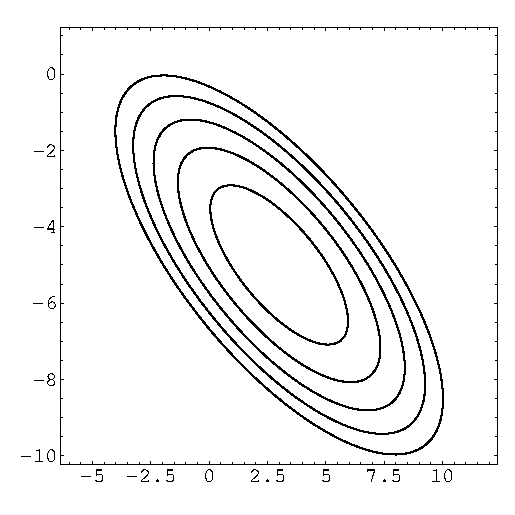
\epsfig{file=kuvat/saari.eps}
\end{center}
\end{figure}
\begin{Exa} Määritä funktion $f(x,y)=x+2y+2$ arvojoukko yksikköneliössä
\[
A=\{(x,y)\in\R^2 \; | \; 0\leq x\leq 1,\; 0\leq y\leq 1\}.
\]
\end{Exa}
\ratk
Tasa-arvokäyrät $S: f(x,y)=c\ $ ovat suoria
%\begin{multicols}{2} \raggedcolumns
\[
x+2y+2=c,
\]
\begin{multicols}{2} \raggedcolumns
joten arvojoukko on (kuva!)
\[
f(A)=[2,5]. \loppu
\]
\begin{figure}[H]
\begin{center}
\import{kuvat/}{kuvaV-1.pstex_t}
\end{center}
\end{figure}
\end{multicols}

\subsection*{Kolmen muuttujan funktiot}
\index{kolmen muuttujan funktio|vahv}

Kolmen reaalimuuttujan funktio on tyyppiä
\[
f:\R^3\kohti\R \quad \text{tai} \quad f:A\kohti\R, \quad A\subset\R^3. 
\]
Kolmen muuttujan funktioita voi havainnollistaa esimerkiksi \pain{vii}p\pain{aloimalla}: 
Valitaan äärellinen joukko muuttujan $z$ arvoja $z_i$ ja tutkitaan kahden muuttujan funktioita
\[
g_i(x,y)=f(x,y,z_i).
\]
\index{zza@\sov!Tomografia}%
\begin{Exa}: \vahv{Tomografia.} \label{tomografia} \ Lääketieteessä paljon käytetyllä 
(tietokone)tomo\-grafialla määritetään nk.\ varjostumafunktio $f$, jonka määrittelyjoukko on
ihmisruumis tai sen osa. Varjostumafunktion arvot ovat reaalilukuja, jotka kertovat
varjostuman tummuusasteen. Funktiosta $f$ saadaan mittausten avulla likimäärin selville
viipaloitujen funktioiden $g_i(x,y)=f(x,y,z_i)$ arvot valituilla (äärellisen monella) $z_i$:n
arvoilla. Funktiot $g_i$ määrätään yhdistämällä suuri joukko erisuuntaisia röntgen(varjo)kuvia 
laskennallisin keinoin (tietokoneen avulla).

Olkoon tarkastelun kohteena (idealisoitu) ihmisen pää
\[
A=\{P \vastaa (x,y,z)\in \R^3 \mid x^2+y^2+z^2\leq 7^2\}
\]
(pituusyksikkö = cm). Tomografiakuvaus tuottakoon varjostumafunktion
\[
f(x,y,z)=1+0.02(2x-3y+6z).
\]
Missä on kirkkainta ja missä tumminta?
\end{Exa}
\ratk Funktio $f$ on saatu käytännössä yhdistelemällä joukko viipalefunktioita
$g_i(x,y)=f(x,y,z_i)$, missä $-7<z_i<7$. Sikäli kuin mittaukset ja niistä lasketut funktiot
$g_i$ ja $f$ katsotaan tarkoiksi, on siis oltava
\[
g_i(x,y)=0.02(2x-3y)+c_i, \quad (x,y) \in A_i\,,
\]
missä $c_i=0.12z_i+1$, ja $A_i$ on kiekon muotoinen leikkauskuvio
\[
A_i=
\{(x,y) \in \R^2 \mid x^2+y^2\leq r_i^2\}, \quad r_i=\sqrt{7^2-z_i^2}.
\]
Funktion $g_i$ tasa-arvokäyrät ovat suoria
\[
2x-3y=\text{vakio},
\]
joten $g_i$:n maksimi ja minimi löytyvät näiden suorien normaalin $3x+2y=0$ ja $A_i$:n 
reunaviivan leikkauspisteistä.
\begin{figure}[H]
\begin{center}
\setlength{\unitlength}{1cm}
\begin{picture}(8,8)(-4,-4)
\put(0,0){\vector(1,0){4}} \put(3.8,-0.4){$x$}
\put(0,0){\vector(0,1){4}} \put(0.2,3.8){$y$}
\put(0,0){\bigcircle{6}}
\multiput(-1,1.5)(1,-1.5){3}{\drawline(-3.5,-2.33)(3.5,2.33)}
\drawline(-2.33,3.5)(2.33,-3.5)
\put(-1.75,2.4){$\bullet$} \put(1.58,-2.6){$\bullet$ $g_i=$max!}
\put(-1.75,3.1){$g_i=$min!}
\put(3,3){$g_i(x,y)=$vakio} \put(2,-4){$3x+2y=0$}
\end{picture}
\end{center}
\end{figure}
Eri viipalekuvia tutkimalla löydetään likimain myös $f$:n maksimi- ja minimiarvot. Tässä
\index{tasa-arvopinta}%
$f$ kuitenkin tunnetaan tarkasti, joten voidaan suoraan tutkia $f$:n \kor{tasa-arvopintoja}.
Nämä ovat tasoja
\[
2x-3y+6z=\text{vakio},
\]
joten voidaan geometrisesti päätellä, että $f$:n maksimi ja minimi löytyvät origon kautta
kulkevan tasa-arvopintojen yhteisen normaalin
\[
\begin{cases} x=2t, \\ y=-3t, \\ z=6t \end{cases}
\]
ja kappaleen reunapinnan
\[
x^2+y^2+z^2=7^2
\]
leikkauspisteistä. Nämä pisteet vastaavat $t$:n arvoja
\[ 
(2t)^2+(-3t)^2+(6t)^2=7^2 \qekv t= \pm 1. 
\]
Varjostuman maksimi- ja minimiarvoiksi päätellään näin muodoin
\begin{alignat*}{3}
&f(2,-3,6)  &\ = 1.98 &= f_{\text{max}}\,, \\
&f(-2,3,-6) &\ = 0.02 &= f_{\text{min}}\,. \qquad\loppu
\end{alignat*}

\subsection*{Funktiot käyräviivaisissa koordinaatistoissa} 
\index{funktio B!h@käyräv.\ koordinaatistoissa|vahv}
\index{muuttujan vaihto (sijoitus)!a@käyräv.\ koordinaatteihin|vahv}
\index{kzyyrzy@käyräviivaiset koordinaatistot!a@--funktiot|vahv}

Kahden ja kolmen reaalimuuttujan funktioita tutkittaessa voi olla apua siirtymisestä 
käyräviivaiseen napa-, lieriö- tai pallokoordinaatistoon silloin kun funktion 
määrittelyjoukon geometria on sellaiseen muunnokseen sopiva. Esimerkiksi, jos kahden
reaalimuuttujan funktio on määritelty pyörähdyssymmetrisessä joukossa $A\subset\Rkaksi$
(voi olla myös $A=\Rkaksi$), voi napakoordinaatteihin siirtyminen auttaa. Siirtyminen tapahtuu
muunnoksella (vrt. Luku \ref{koordinaatistot})
\begin{multicols}{2} \raggedcolumns
\begin{align*}
f(x,y)&=f(r\cos\varphi,r\sin\varphi) \\[2mm]
      &=g(r,\varphi).
\end{align*}
\begin{figure}[H]
\setlength{\unitlength}{1cm}
\begin{center}
\begin{picture}(4,3)(-1,0)
\put(-1,0){\vector(1,0){4}} \put(2.8,-0.4){$x$}
\put(0,0){\vector(0,1){3}} \put(0.2,2.8){$y$}
\put(0,0){\vector(2,3){1.5}}
\arc{1}{5.25}{6.2}
\put(0.5,1.1){$r$} \put(0.5,0.25){$\varphi$} \put(1.45,2.15){$\bullet$ $(x,y)$}
\end{picture}
\end{center}
\end{figure}
\end{multicols}
Huomattakoon, että muunnettu funktio $g$ on itse asiassa yhdistetty funktio
\[
g(r,\varphi)=f(x(r,\varphi),y(r,\varphi)),
\]
missä $x(r,\varphi)=r\cos\varphi,\ y(r,\varphi)=r\sin\varphi$. Siirtyminen 
polaarikoordinaatistosta karteesiseen tapahtuu käänteismuunnoksella
\[
f(x,y)=g(r(x,y),\varphi(x,y)),
\]
missä $\,r(x,y)=\sqrt{x^2+y^2}\,$ ja $\,\varphi(x,y)\,$ on pistettä $(x,y)$ vastaava 
napakulma\footnote[2]{Merkinnöissä $x(r,\varphi)$, $y(r,\varphi)$, $r(x,y)$ ja $\varphi(x,y)$
on alunperin riippumattomista muuttujista $x,y$ tai $r,\varphi$ tehty funktiosymboleja.
Koordinaattimuunnoksissa (myös implisiittifunktioissa, vrt.\ edellinen luku) tällaiset
merkinnät ovat tavallisia, koska ne selkeyttävät laskemista.}
($\varphi$:n laskukaava on hieman konstikas, ks.\ edellisen luvun Esimerkki 
\ref{napakulman kaava}).

Kolmen muuttujan funktioita tarkasteltaessa voidaan siirtyä lieriö- tai 
pallokoordinaatistoon muunnoksilla
\begin{align*}
\text{Lieriö:} \quad  f(x,y,z) &= f(r\cos\varphi,r\sin\varphi,z) =g(r,\varphi,z). \\
\text{Pallo:} \quad\  f(x,y,z) &= f(r\sin\theta\cos\varphi,r\sin\theta\sin\varphi,r\cos\theta)
                                = g(r,\theta,\varphi).
\end{align*}
Lieriökoordinaatiston tapauksessa muunnos $(x,y)\ext(r,\varphi)$, samoin käänteismuunnos
$(r,\varphi)\ext(x,y)$ on sama kuin napakoordinaatistossa. Pallokoordinaatistossa 
käänteismuunnos on
\begin{align*}
g(r,\theta,\varphi) &= g(r(x,y,z),\theta(x,y,z),\varphi(x,y)) \\
&=f(x,y,z),
\end{align*}
missä
\begin{align*}
     r(x,y,z) &= \sqrt{x^2+y^2+z^2}, \\
\theta(x,y,z) &= \Arccos\left(\frac{z}{\sqrt{x^2+y^2+z^2}}\right),
\end{align*}
ja $\varphi(x,y)$ on sama kuin napakoordinaatistossa. Suuntakulma $\theta$ ei ole määritelty
origossa eikä kulma $\varphi$ $z$-akselilla.
\begin{Exa}
Vuoristoisen maaston korkeus merenpinnasta on origon ympäristössä
\[
f(x,y)=x^2-2xy-3y^2+0.2x-0.1y+10
\]
(yksikkö = 100 m). Origossa on kahden tien risteys. Tiet ovat kartalla suoria ja myös niiden
sivuprofiili on suora. Mihin suuntiin tiet kulkevat ja mikä on teiden kaltevuus?
\end{Exa}
\ratk
Siirrytään napakoordinaatistoon:
\[
f(x,y)=h(r,\varphi)=r^2(\cos^2 \varphi-2\cos\varphi\sin\varphi-3\sin^2\varphi) 
                                      + r(0.2\cos\varphi-0.1\sin\varphi) +10.
\]
Tiet noudattavat origosta lähdettäessä puolisuoria $\varphi=\varphi_1$ ja $\varphi=\varphi_2$
(koska ovat kartalla suoria). Koska teiden sivuprofiilikin on suora, on oltava
\[
\cos^2 \varphi-2\cos\varphi\sin\varphi-3\sin^2\varphi=0.
\]
Tässä ei $\,\cos\varphi=0\,$ ole ratkaisu, joten voidaan jakaa $\cos^2\varphi$:lla:
\[
1-2\tan\varphi-3\tan^2\varphi=0 
           \qekv \begin{cases}
                  \,\tan\varphi_1=1/3 \ & \impl \ \ \varphi_1 \approx 18\aste\ 
                                                              \text{tai}\ 198\aste, \\
                  \,\tan\varphi_2=-1 \  & \impl \ \ \varphi_2 =135\aste\
                                                              \text{tai}\ 315\aste.
                  \end{cases}
\]
Kaltevuuskulmat suuntiin $\varphi_1 \approx 18\aste$ ja $\varphi_2=135\aste$ saadaan
ratkaisemalla
\[
\tan\alpha_i=0.2\cos\varphi_i-0.1\sin\varphi_i
                  \qimpl \begin{cases}
                         \,\alpha_1\approx 9\aste, \\
                         \,\alpha_2\approx -12\aste.
                         \end{cases} \qquad\loppu
\]

\begin{Exa}
Etsi (jos mahdollista) pisteet, joissa funktio
\[
f(x,y,z)=xyz(3x^2+3y^2-z^2)/(x^2+y^2)
\]
saavuttaa maksimi- tai minimiarvonsa joukossa
\[
A=\{(x,y,z)\in\R^3 \ | \ x^2+y^2+z^2\leq 96, \ (x,y)\neq (0,0)\}.
\]
\end{Exa}
\ratk Siirrytään pallokoordinaatistoon. Koska pallokoordinaateissa on
\[
x^2+y^2=r^2\sin^2\theta(\cos^2\varphi + \sin^2\varphi)=r^2\sin^2\theta,
\]
niin (vrt.\ Luku \ref{trigonometriset funktiot})
\begin{align*}
f(x,y,z)\,=\,g(r,\theta,\varphi) 
         &=\,r^3\cos\theta\,(3\sin^2\theta-\cos^2\theta)\cos\varphi\sin\varphi \\[2mm]
         &=\,r^3\,(3\cos\theta-4\cos^3\theta)\cos\varphi\sin\varphi \\
         &=-\frac{1}{2}\,r^3\cos 3\theta\sin 2\varphi.
\end{align*}
Funktio $g$ saavuttaa maksimiarvonsa $192\sqrt{6}$ pallon pinnalla $(r=\sqrt{96}=4\sqrt{6})$, 
kun joko $\cos 3\theta=-1$, $\sin 2\varphi=1$ tai $\cos 3\theta=1$, $\sin 2\varphi=-1$. 
Maksimikohtia on neljä:
\[
\begin{array}{llllrr}
(r, & \theta, & \varphi) & (x, & y, & z) \\ \\
(4\sqrt{6}, & \pi/3, & \pi/4) \quad & (\ \: \, 6, &6, &2\sqrt{6}) \\ 
(4\sqrt{6}, & \pi/3, & 5\pi/4) \quad & (-6, &-6, &2\sqrt{6}) \\ 
(4\sqrt{6}, & 2\pi/3, & 3\pi/4) \quad & (-6, & 6, &-2\sqrt{6}) \\ 
(4\sqrt{6}, & 2\pi/3, & 7\pi/4) \quad & (\ \: \, 6, &-6, &-2\sqrt{6})
\end{array}
\]
Minimikohtia (joissa $g=g_{\text{min}}=-192\sqrt{6}$) on samoin neljä. Nämä saadaan vaihtamalla
yhden koordinaatin merkki maksimipisteiden karteesisessa esitysmuodossa. Funktio $g$ saavuttaa
maksimi- tai minimiarvonsa myös pallonpintakoordinaattien arvoilla 
$(\theta,\varphi) \in  \{0,\pi\} \times \{\pi/4,\ 3\pi/4,\ 5\pi/4,\ 7\pi/4\}$. Nämä vastaavat 
kuitenkin karteesisen koordinaatiston pisteitä $(0,0,z)$, jotka ovat alkuperäisen funktion $f$ 
määrittelyjoukon ulkopuolella. \loppu

\subsection*{Usean muuttujan funktioiden yhdistely}
\index{funktio B!e@yhdistetty|vahv}
\index{yhdistetty funktio|vahv}

Useamman reaalimuuttujan reaaliarvoisia funktioita voi yhdistellä yhdistetyiksi funktioiksi 
samoilla periaatteilla kuin yhden muuttujan tapauksessa. Lisäehtona on kuitenkin, että funktiot
ovat tyypiltään yhteensopivia. Esimerkiksi funktioiden $f(x)$ ja $g(x,y)$ yhdistetty funktio 
$F = f \circ g$  voidaan määritellä: 
\[ 
F(x,y) = (f \circ g)(x,y) = f(g(x,y)), \quad \DF_F = \{(x,y) \in \DF_g \mid g(x,y) \in \DF_f\}.
\]
Voidaan myös määritellä yhdistetyt funktiot
\begin{align*}
&G_1(x) = g(x,f(x)),   \quad \DF_{G_1} = \{x \in \DF_f \mid (x,f(x)) \in \DF_g\}, \\
&G_2(y) = g(f(y),y), \,\quad \DF_{G_2} = \{y \in \DF_f \mid (f(y),y)\,\in \DF_g\}, \\
&G_3(x,y) = g(f(x),f(y)),\quad \DF_{G_3} 
                               = \{(x,y) \in \DF_f \times \DF_f \mid (f(x),f(y)) \in \DF_g\}.
\end{align*}
Funktiota $g \circ f$ sen sijaan ei voi määritellä, ei myöskään funktiota $g \circ g$.
\begin{Exa} Jos $f(x) = \sqrt{x},\ \DF_f = [0,\infty)$ ja $g(x,y) = x-y^2,\ \DF_g = \R^2$, niin
\begin{align*}
&F(x,y) = (f \circ g)(x,y) = \sqrt{x-y^2}, \quad \DF_F = \{(x,y) \in \R^2 \mid x \ge y^2\}, \\
&G(x) = g(x,f(x)) = 0, \quad \DF_G = [0,\infty). \loppu
\end{align*} \end{Exa}
\begin{Exa} Määritä funktion $f(x,y) = x^2 + 2y^2 + 2xy + 4x + 14y$ minimiarvo suoralla 
$S:\ y = 2x-5$. (Vrt.\ Esimerkki \ref{saari}.) \end{Exa}
\ratk Kun käytetään suoralla $S$ vallitsevalle funktioriippuvuudelle $x \map y$ 
merkintää $y(x)$, niin kyse on yhdistetystä funktiosta $F(x) = f(x,y(x))$, $\DF_F = \R$.
Koska
\begin{align*}
 F(x) = f(x,2x-5) &= x^2 + 2(2x-5)^2 + 2x(2x-5) + 4x + 14(2x-5) \\[3mm]
                  &= 13x^2 - 18x - 20 \\
                  &= 13\left(x-\dfrac{9}{13}\right)^2 - \dfrac{341}{13}\,,
\end{align*}
niin nähdään, että kysytty minimiarvo on
\[ 
F_{\text{min}} = -\dfrac{341}{13} \approx -26.2. 
\]
Minimikohta on suoran pisteessä $(9/13,-47/13) \approx (0.69,-3.62)$. \loppu

Useamman muuttujan funktioita voidaan yhdistellä myös laskutoimituksin samalla tavoin kuin
yhden muuttujan funktioita (Määritelmä \ref{funktioiden yhdistelysäännöt}).  Ellei
yhdisteltävien funktioiden muuttujien lukumäärä täsmää, on ajateltava, että funktioissa on 
'näkymättömiä' muuttujia. 
\begin{Exa} Jos $f(x) = \tan x\,$ ja $\,g(x,y) = \sin(x+y^2)$, niin kirjoitettaessa
\[ 
F(x,y) = \tan x + \sin (x+y^2) 
\]
tarkoitetaan tämän laskusäännön ilmaisemaa funktiota $F$, määrittelyjoukkona 
\[ 
\DF_F = \{(x,y) \in \R^2 \mid x \neq (n+1/2)\,\pi\,\ \forall n \in \Z\}.
\]
Samaan tulokseen tullaan myös funktioiden yhdistelyn kautta ajattelemalla, että
$F = \tilde{f} + g,\ \DF_F = \DF_{\tilde{f}} \cap \DF_g$, missä $\tilde{f}$ on saatu $f$:stä
lisäämällä toinen muuttuja:
\[ 
\tilde{f}(x,y) = \tan x, \quad \DF_{\tilde{f}} = \DF_f \times \R. \loppu
\] 
\end{Exa}

\subsection*{Kahden muuttujan implisiittifunktiot}
\index{funktio B!j@implisiittifunktio|vahv}
\index{implisiittifunktio|vahv}

Jos $F$ on kolmen muuttujan funktio ja yhtälö
\[
F(x,y,z)=0
\]
ratkeaa $z$:n suhteen, kun $(x,y)\in A\subset\R^2$, niin yhtälö määrittelee $A$:ssa
kahden muuttujan (mahdollisesti monihaaraisen) implisiittifunktion. Jos tälle käytetään
funktiomerkintää $z(x,y)$, niin määritelmä on siis
\[
F(x,y,z(x,y))=0, \quad (x,y)\in A.
\]
\begin{Exa}
Yhtälö $x^2+y^2+z^2=R^2$ määrittelee kaksihaaraisen implisiittifunktion
$z(x,y)=\pm\sqrt{R^2-x^2-y^2}\,$ kiekossa $A:\ x^2+y^2 \le R^2$. \loppu
\end{Exa}
\begin{Exa} Jos $m\in\N,\ m \ge 2$, niin yhtälö
\[
y,z\in\C: \quad y^m=z
\]
määrittelee $m$-haaraisen kompleksifunktion $y=\sqrt[m]{z}$, vrt.\ Luku \ref{III-3}.
Jos kirjoitetaan $z=x+iy$ ja $y=u(x,y)+iv(x,y)$, niin $u$ ja $v$ ovat $m$-haaraisia
funktioita tyyppiä $u,v:\ \Rkaksi\kohti\R$. \loppu
\end{Exa}

\Harj
\begin{enumerate}

\item
Määritä seuraavien funktioiden arvojoukot annetulla janalla $AB$\,: \newline
a) \ $f(x,y)=x^2+2xy-y^2,\,\ A=(1,2),\ B=(-1,3)$ \newline
b) \ $f(x,y,z)=x+xy+yz+z^2,\,\ A=(1,1,1),\ B=(-1,2,-3)$

\item
Määritä seuraavien funktioiden arvojoukot annetussa joukossa $A$: \newline
a) \ $f(x,y)=x+3y-1$, \ $A=$ kolmio, jonka kärjet $(0,1)$, $(4,0)$ ja $(3,4)$ \newline
b) \ $f(x,y,z)=x+2y-3z$, \ $A=\{(x,y,z) \mid (x-1)^2+(y+1)^2+(z-2)^2 \le 9\}$ \newline
c) \ $f(x,y,z)=x+xy+yz+z^2$, \ $A=$ suora $\,2x-2=y+1=4-2z$

\item
Tasangolla $z=0$ on järvi $A=\{(x,y)\in\Rkaksi \mid h(x,y)<0\}$, missä
\[
h(x,y) = 4x^2+y^2+24x+8y
\]
on järven pohjan korkeusprofiili. Tässä $h$ on ilmaistu metreinä ja $x,y$ kilometreinä.
Järven poikki kulkee moottoritie suoraa $y=x+2$ pitkin. Missä on järven syvin kohta ja mikä
on syvyys tässä kohdassa? Hahmottele järven rantaviiva ja laske, missä pisteissä moottoritie
leikkaa rantaviivan.

\item
Muunna seuraavat funktiot napa- tai pallokoordinaatistoon:
\begin{align*}
&\text{a)}\ \ f(x,y)=x+2y \qquad \text{b)}\ \ f(x,y)=xy^2 \qquad 
 \text{c)}\ \ f(x,y)=\frac{xy}{x^2+y^2} \\
&\text{d)}\ \ f(x,y)=\max\{0,x,y\} \qquad
 \text{e)}\ \ f(x,y)=\begin{cases} x^2/y, &\text{kun}\ x > 0\ \text{ja}\ y>0 \\
                                   0,     &\text{muulloin}
                     \end{cases} \\
&\text{f)}\ \ f(x,y)=\begin{cases} xy^2-y^3, &\text{kun}\ 0 \le x \le y \\
                                   0,        &\text{muulloin}
                     \end{cases} \qquad
 \text{g)}\ \ f(x,y,z)=\frac{xyz}{x^2+y^2+z^2} \\
&\text{h)}\ \ f(x,y,z)=\frac{xy^2z^3}{x^2+y^2} \qquad 
 \text{i)}\ \ f(x,y,z)=\begin{cases}
                      \,z^2-xyz, &\text{kun}\ z>0 \\ \,0, &\text{kun}\ z \le 0
                      \end{cases}
\end{align*}

\item
Muunna seuraavat napakoordinaateissa ilmaistut funktiot karteesiseen koordinaatistoon:
\begin{align*}
&\text{a)}\ \ g(r,\varphi)=r^3(\cos\varphi-\sin\varphi) \qquad
 \text{b)}\ \ g(r,\varphi)=\sin 2\varphi-r^2\cos 2\varphi \\
&\text{c)}\ \ g(r,\varphi)=r^2(\tan\varphi+\cot\varphi) \qquad
 \text{c)}\ \ g(r,\varphi)=\frac{\sin\varphi}{2+\cos\varphi}
\end{align*}

\item
Olkoon $f(x,y)=x+y$ ja $g(x,y)=xy,\ (x,y)\in\Rkaksi$. Määrittele sievennettyinä lausekkeina 
(laskusääntöinä) seuraavat yhdistetyt funktiot: \newline
a) \ $f(x,g(x,y))\quad$ b) \ $f(g(x,y),y)\quad$ c) \ $f(g(x,y),g(x,y))$ \newline
d) \ $g(x,f(x,y))\quad$ e) \ $g(f(x,y),y)\quad$ f) \ $g(f(x,y),f(x,y))$ \newline
g) \ $f(f(x,y),f(x,y))\quad$ h) \ $g(g(x,y),g(x,y))$

\item
Olkoon $f(x)=\sqrt{2-x}$ ja $g(x,y)=\sqrt{x-y^2}\ (x,y\in\R)$. Määrittele yhdistetty funktio
$F=f \circ g$ (laskusääntö ja määrittelyjoukko).

\item
Olkoon $f(x)=\sqrt{25-x^2}$ ja $g(x,y)=3x+4y-1\ (x,y\in\R)$. Määritä yhdistetyn funktion
$F=f \circ g$ pienin ja suurin arvo yksikkökiekon neljänneksessä
$A= \{\,(x,y)\in\Rkaksi \mid x \ge 0\,\ja\,y \ge 0\,\ja\,x^2+y^2 \le 1\,\}$.

\item
a) Esitä kompleksifunktion $f(z)=(z+1)^2+(z+i)^2$ reaaliosa, imaginaariosa ja itseisarvo
funktioina tyyppiä $g:\ \Rkaksi \kohti \R$. \vspace{1mm}\newline
b) Määrittele kaksihaaraiset funktiot $u=\{u_1,u_2\}$ ja $v=\{v_1,v_2\}$ siten, että
$u(x,y)+iv(x,y)=\sqrt{z}\ \ \forall z=x+iy\in\C$.

\item
Yhtälö $x+3xyz^2+z^4=0\ (x,y,z\in\R)$ määrittelee implisiittifunktion $z=f(x,y)$. \ a) Laske 
$f$:n arvot pisteissä $(0,0)$, $(2,-1)$ ja $(1,1)$. \ b)  Millaisia ovat $f$:n haarat 
(määrittelyjoukot ja laskusäännöt) yleisemmin?

\item (*)
Vuoristoisen maaston korkeus merenpinnasta on origon $O$ lähellä funktio
\[
f(x,y)=\frac{1}{20}(3x^2-5xy-2y^2)+2.
\]
Origossa on kahden tien $S_1,S_2$ risteys. Tiet ovat maastoon sovitettuja ja vaakasuoria, ja 
lisäksi ne ovat kartallakin suoria. Teiden $S_1,S_2$ poikki kulkee suora rautatie pisteissä
$A\in S_1$, $B\in S_2$. Molemmat pisteet ovat $O$:sta etäisyydellä $1$ (yksikkö = km).
Mikä on suurin pudotuskorkeus laaksoon rautatiesillalta, jonka päät ovat pisteissä $A,B$\,?

\item (*)
Halutaan selvittää, missä pisteissä funktio $f(x,y)=x^2-2xy+3y^2$ saavuttaa suurimman ja 
pienimmän arvonsa\, a) ympyrällä \mbox{$S: x^2+y^2=9$}, \ \ b) kiekossa 
$A=\{(x,y)\in\Rkaksi \mid x^2+y^2 \le 9\}$. Ratkaise ongelma napakoordinaatteja käyttäen 
(vrt.\ Harj.teht.\,\ref{trigonometriset funktiot}:\ref{H-II-5: minmax}).

\item (*)
Funktiosta $f(x)=x-x^3\,$ tiedetään, että välillä $[0,1]$ $f$ saavuttaa suurimman arvonsa
pisteessä $x=1/\sqrt{3}$. Mihin suuntaan origosta lähdettäessä funktio\, a) $f(x,y)=xy^2$,\,
b) $f(x,y,z)=xy^2z^3$ kasvaa nopeimmin suhteessa kuljettuun matkaan?

\item (*) \index{zzb@\nim!Funktio avaimenreiässä} 
(Funktio avaimenreiässä) Olkoon
\[
A=\{\,(x,y,z)\in \R^3 \mid (x,y)\in B_1 \cup B_2,\,\ z\in[0,10]\,\},
\]
missä 
\begin{align*}
B_1 &= \{\,(x,y)\in\Rkaksi \mid x^2+(y-1)^2 \le 2\,\ja\, y \ge 0\,\}, \\
B_2 &= \{\,(x,y)\in\Rkaksi \mid x\in[-1,1]\,\ja\,y\in [-4,0]\,\}.
\end{align*}
Missä $A$:n pisteissä funktio $f(x,y,z)=x-3y+2z$ saavuttaa suurimman ja missä pienimmän arvonsa?

\end{enumerate}


\section{Parametriset k�yr�t ja pinnat} \label{parametriset k�yr�t}
\alku
\index{funktio A!f@parametrinen k�yr� ja pinta|vahv}
\index{parametrinen k�yr�|vahv}
\index{parametri(sointi)!c@k�yr�n|vahv}
\index{kzyyrzy@k�yr�|vahv}

Tason tai avaruuden \kor{parametriseksi k�yr�ksi} sanotaan \pain{funktiota} muotoa
\[ 
t \in A\ \map\ P(t)\in E^d, 
\]
miss� $A \subset \R$ on \pain{v�li} (usein suljettu v�li) ja $d=2$ tai $d=3$. Muuttujaa $t$ 
sanotaan t�ss� \kor{parametriksi}. K�yr� on \kor{tasok�yr�} jos $d=2$, \kor{avaruusk�yr�} jos 
$d=3$. K�ytt�en jo tutuksi tulleita geometrisia vastaavuuksia voidaan kirjoittaa
\[
P(t)\ \vastaa\ \Vect{OP}(t)\ 
                = \left\{ \begin{array}{lrlll} 
                   x(t)\vec{i}+y(t)\vec{j} & \vastaa & (x(t),y(t)),      & & (d=2) \\
                   x(t)\vec{i}+y(t)\vec{j}+z(t)\vec{k} & \vastaa & (x(t),y(t),z(t)), & & (d=3)
                          \end{array} \right.
\]
miss� $x,y,z$ ovat funktioita tyyppi� $f: A \kohti \R$. T�m�n mukaisesti parametrinen k�yr� 
\index{vektoric@vektoriarvoinen funktio}%
voidaan tulkita reaalimuuttujan \kor{vektoriarvoiseksi} funktioksi, jolloin luonteva esitystapa
on my�s vektorimerkint�
\[ 
\vec{r}\,(t)\ =\ \begin{cases} 
   x(t)\vec{i}+y(t)\vec{j},\ \ t \in A,                   &\text{(tasok�yr�)} \\
   x(t)\vec{i}+y(t)\vec{j}+z(t)\vec{k},\ \ t \in A. \quad &\text{(avaruusk�yr�)}
               \end{cases}
\]
Liittyen vastaavuuteen $\mathit{E^d} \vast \R^d$ voidaan parametrinen k�yr� esitt�� yht� hyvin 
yht�l�ryhm�n�, esim.\ tasok�yr�n tapauksessa
\[ 
(x,y)\ =\ (x(t),y(t)) \qekv 
        \begin{cases} \,x = x(t), \\ \,y = y(t). \end{cases} \quad 
\text{(tasok�yr�)}\footnote[2]{Merkinn�iss� $x=x(t)$ ja $y=y(t)$ on symboleja $x,y$ k�ytetty
kahdessa eri merkityksess�: oikealla funktion, vasemmalla ko.\ funktion arvojoukon alkion
symbolina. T�m�n tyyppisi� ep�loogisuuksia pidet��n matematiikan k�yt�nn�ss� siedett�vin�,
syyst� ett� ne yksinkertaistavat merkint�j�.}
\]
\begin{Exa} Reaalimuuttujan funktio $f: [a,b] \kohti \R$ voidaan tulkita parametriseksi
tasok�yr�ksi
\[ 
\vec{r} = \vec{r}\,(t) = t\vec{i} + f(t)\vec{j} \qekv 
                           \begin{cases} \,x = x(t) = t, \\ \,y = y(t) = f(t),\ \ t \in [a,b]. 
                           \end{cases} \loppu 
\] 
\end{Exa}
\begin{Exa} Luvuista \ref{suorat ja tasot} ja \ref{koordinaatistot} tuttuja parametrisia 
avaruusk�yri� ovat
\begin{align*}
&\text{avaruussuora:}\quad \vec{r}\,(t)\ 
          =\ (x_0 + \alpha t)\vec{i} + (y_0 + \beta t)\vec{j} + (z_0 + \gamma t)\vec{k}\ 
          =\ \vec{r}_0 + t \vec{v}, \quad t \in \R, \\ 
&\text{ruuviviiva:}\quad \begin{cases}
                          \,x = x(\varphi) = R\cos\varphi, \\ 
                          \,y = y(\varphi) = R\sin\varphi, \\ 
                          \,z = z(\varphi) = a\varphi,\ \ \varphi \in \R. \loppu
                         \end{cases} 
\end{align*} 
\end{Exa}
Parametrisen k�yr�n euklidiseen avaruuteen j�tt�m� 'geometrinen j�lki' on arvojoukko 
$S = \{P(t) \vastaa \vec{r}\,(t) \mid t \in A\} \subset E^d$, johon voidaan viitata sellaisilla 
termeill� kuin \kor{k�yr�} (engl.\ curve) tai (k�yr�n) \kor{kaari} (engl.\ arc). 
Yksinkertaisimmillaan $S$ on jostakin pisteest� $A$ alkava ja toiseen pisteeseen $B$ p��ttyv�,
\index{yksinkertainen!c@k�yr�, kaari} \index{kaari (k�yr�n)}%
itse��n leikkaamaton ja yhten�inen viiva, eli nk.\ \kor{yksinkertainen kaari} (engl.\ 
simple arc). T�llaisia ovat esim.\ jana tai ympyr�n kaari. Viiva voi my�s olla p��ttym�t�n, 
kuten suora, tai umpinainen
\index{suljettu k�yr�}%
\kor{suljettu k�yr�} (engl.\ closed curve), kuten tason tai 
avaruuden ympyr�viiva. Joukko $S$ voi my�s olla itse��n leikkaava, eli siin� voi olla 
'silmukoita'.\footnote[2]{Muodossa $S = \{P(t) \vastaa \vec{r}\,(t) \mid t \in A\}$
m��riteltyjen taso- tai avaruusk�yrien geometrista luokittelua ei todellisuudessa voi
t�sment�� ilman funktion $\vec{r}$ koordinaattifunktioile $x,y,z$ asetettavia lis�ehtoja.
Vrt.\ k�yri� koskeva alaviite edellisess� luvussa.}
Jos l�ht�kohdaksi otetaan vain t�llainen 'viiva' $S$, eli pelk�st��n geometrinen objekti, niin 
funktiota $\vec{r}\,(t),\ t \in A$, jonka arvojoukko $=S$, sanotaan $S$:n 
\kor{parametriesitykseksi} eli \kor{parametrisoinniksi} (parametrisaatioksi). 
Parametrisoivan funktion $t \in A \map \vec{r}\,(t) \in S$ ei tarvitse olla injektiivinen, ts.\ 
samaan pisteeseen $P \in S$ voidaan p��ty� monella (jopa ��rett�m�n monella) parametrin
arvolla.
\begin{Exa} \label{ympyr�n parametrisaatio} Tason ympyr�viivan 
\[ 
S = \{P \vastaa (x,y) \in \R^2 \mid (x-x_0)^2 + (y-y_0)^2 = R^2\} 
\]
luonteva parametrisointi on
\[ 
\begin{cases} x = x_0 + R \cos t, \\ y = y_0 + R\,\sin t,\ \ t \in [0,2\pi). \end{cases} 
\]
T�ss� voi v�lin $[0,2\pi)$ tilalla olla my�s esim.\ $A = (-\pi,\pi]$, $A = [0,2\pi]$ tai
$A = \R$. Kahdessa j�lkimm�isess� vaihtoehdossa parametrisointi ei ole injektio. \loppu
\end{Exa}
\begin{Exa} Jos $S$ on avaruussuora, niin t�m�n tavanomaisin parametrisaatio on 
$\vec{r}\,(t) = \vec{r}_0 + t \vec{v},\ t \in \R$, miss� $P_0 \vastaa \vec{r}_0$ on suoran
piste ja $\vec{v} \neq \vec{0}$ suoran suuntavektori (vrt.\ Luku \ref{suorat ja tasot}).
T�llaisiakin parametrisointeja on jo ��rett�m�n monta, mutta mahdollisuudet eiv�t lopu t�h�n:
Jos $\vec{r}_0$ ja $\vec{v}$ t�ytt�v�t mainitut ehdot, niin parametrisoinniksi voidaan
yleisemmin valita
\[ 
\vec{r}\,(t)\ =\ \vec{r}_0 + f(t)\,\vec{v}, \quad t \in A, 
\]
miss� funktion $f: A \kohti \R$ valintaa rajoittaa vain ehto $\RF_f = \R$. Esimerkiksi voidaan 
valita $f(t) = \tan t,\ A = (-\pi/2,\pi/2)$ ($f$ injektio), tai $f(t) = t \sin t,\ A = \R$ 
($f$ ei injektio).  \loppu \end{Exa}
\jatko \begin{Exa} (jatko) Jos halutaan parametrisoida suoralla $S$ oleva jana, jonka 
p��tepisteet ovat $A \vastaa \vec{r}_1$ ja $B \vastaa \vec{r}_2$, niin t�m� k�y muodossa
\[ 
\vec{r}\,(t) = f(t)\,\vec{r}_1 + [1-f(t)]\,\vec{r}_2,\ \ t \in A, 
\]
miss� $f$ on funktio tyyppi� $f: A \kohti \R,\ A \subset \R$, ja $\RF_f = [0,1]$.
Yksinkertaisin parametrisointi saadaan, kun valitaan $A = [0,1]$ ja $f(t) = t$. \loppu 
\end{Exa}
Jos tasok�yr�n yht�l�ist� $x = x(t),\ y = y(t),\ t \in A$ pystyt��n eliminoimaan parametri
$t$, on tuloksena yht�l� muotoa
\[ 
F(x,y) = 0, 
\]
miss� siis $F$ on kahden muuttujan funktio, jolle p�tee $F(x(t),y(t)) = 0\,\ \forall t \in A$.
Jos $S = \{P \in \Ekaksi \mid P \vastaa (x(t),y(t))\ \text{jollakin}\ t \in A\}$, niin
sanotaan t�ll�in, ett� ym.\ yht�l� on \kor{k�yr�n} $S$ (tai pistejoukon $S$) \kor{yht�l�}.
Avaruusk�yr�n tapauksessa johtaa parametrin eliminointi (onnistuessaan) yht�l�ryhm��n muotoa
\[ 
\begin{cases} \,F_1(x,y,z) = 0, \\ \,F_2(x,y,z) = 0. \end{cases} 
\]
\begin{Exa} Jos $a,b>0$, niin parametrinen tasok�yr�
\[ 
S:\ \begin{cases} \,x = a\cos t, \\ \,y = b\,\sin t,\ \ t \in [0,2\pi] \end{cases} 
\]
on nimelt��n \kor{ellipsi} (tapauksessa $a=b$ ympyr�). Eliminoimalla $t$ saadaan $S$:n
yht�l�ksi
\[ 
\frac{x^2}{a^2} + \frac{y^2}{b^2} = 1. \loppu
\]
\end{Exa}

\subsection*{Liikerata}
\index{liikerata|vahv}

Tyypillisess� parametrisen k�yr�n fysikaalisessa sovellustilanteessa parametri $t$ on 
\pain{aika}muuttuja, $A$ on tarkasteltava \pain{aikav�li}, ja $P(t) \vastaa \vec{r}\,(t)$ on 
liikkuvan pisteen (esim.\ pistem�iseksi ajatellun partikkelin tai liikkuvan kiinte�n kappaleen 
pisteen) p\pain{aikka} hetkell� $t$. T�ll�in funktion $P(t),\ t \in A$, arvojoukko $S$ on ko.\
pisteen \pain{liikerata} aikav�lill� $A$. Funktio $t\map\vec r\,(t),\ t \in A$ on $S$:n
parametrisointi, joka kertoo koko \pain{liikehistorian}. 
\index{zza@\sov!Heittoparaabeli}%
\begin{Exa}: \vahv{Heittoparaabeli}. \label{heittoparaabeli}
Kivi heitet��n tornista korkeudelta $h$ alkuvauhdilla $v_0$ ja kulmassa $\alpha$ vaakasuuntaan
n�hden. Millainen on lentorata, jos ilmanvastusta ei huomioida?
\end{Exa}
\ratk Tarkastellaan liikett� (avaruustason) koordinaatistossa, jossa $x$ mittaa vaakasuoraa
et�isyytt� l�ht�pisteest� ja $y$ korkeutta maan pinnan tasosta. Liikelakien mukaan kiven
paikka $P(t)=(x(t),y(t))$ on lentoajan $t$ funktiona parametrinen k�yr�
\[
\begin{cases}
\,x(t)=v_0t\cos\alpha, \\
\,y(t)=h+v_0t\sin\alpha-\tfrac{1}{2}gt^2,
\end{cases}
\]
miss� $g=$ maan vetovoiman kiihtyvyys. Eliminoimalla $t$ ja huomioimalla, ett�
$1/\cos^2\alpha=1+\tan^2\alpha\,$ saadaan lentoradan yht�l� muotoon
\[
y=h+kx-(1+k^2)\frac{x^2}{2a}\,,
\]
\index{paraabeli}%
miss� $\,k=\tan\alpha\,$ ja $\,a=v_0^2/g$. Lentorata on \kor{paraabelin} kaari. Kuvan
tapauksessa $\alpha=0$ kivi t�rm�� maahan hetkell� $t=\sqrt{2h/g}$. \loppu
\begin{figure}[H]
\setlength{\unitlength}{1cm}
\begin{center}
\begin{picture}(8,5)(0,0)
\put(0,0){\vector(1,0){8}} \put(7.8,-0.5){$x$}
\put(1,0){\vector(0,1){5}} \put(1.2,4.8){$y$}
\linethickness{0.05cm}
\multiput(0,0)(1,0){2}{\line(0,1){3.7}}
\multiput(0,3.7)(0.4,0){3}{\line(1,0){0.2}}
\multiput(0.2,3.7)(0.2,0){4}{\line(0,-1){0.2}}
\multiput(0.2,3.5)(0.4,0){2}{\line(1,0){0.2}}
\thinlines
\curve(1,3.7,4,2.8,6,0)
\end{picture}
\end{center}
\end{figure}
\index{zza@\sov!Sykloidi}%
\begin{Exa}: \vahv{Sykloidi}. \label{sykloidi}
$R$-s�teinen py�r� vierii liukumatta pitkin tasoa siten, ett� py�r�n keskipisteen liikenopeus
on $v_0\vec i$, $v_0=\text{vakio}$. M��rit� py�r�n ulkokeh�n pisteen $P$ paikka ajan $t$
funktioina.
\end{Exa}
\ratk Oletetaan, ett� py�r� vierii pitkin $x$-akselia ja ett� $P$ on origossa, kun $t=0$. 
T�ll�in ratak�yr�n parametriesitys on
\begin{multicols}{2} \raggedcolumns
\[
\begin{cases} x(t) = v_0t-R\sin \varphi(t), \\ y(t) = R-R\cos \varphi(t), \end{cases}
\]

\vspace{1mm}

miss� $\varphi(t)$ on vierimiskulma. 

\begin{figure}[H]
\setlength{\unitlength}{1cm}
\begin{center}
\begin{picture}(5,3)(-1,0)
\put(0,0){\vector(1,0){4}} \put(3.8,-0.5){$x$}
\put(0,0){\vector(0,1){3}} \put(0.2,2.8){$y$}
\put(2,1.25){\circle{2.5}}
\dashline{0.2}(0,2.5)(4,2.5) \put(-0.5,2.4){$\scriptstyle{2R}$}
\dashline{0.1}(2,1.25)(0.8,1.6)
\put(2,1.25){\vector(1,0){1}} \put(2.6,1.4){$\scriptstyle{v_0\vec i}$}
\dashline{0.1}(2,0)(2,1.25)
\put(2,1.25){\arc{0.6}{1.59}{3.43}}
\put(1.2,0.85){$\scriptstyle{\varphi(t)}$}
\put(1.93,1.18){$\scriptstyle{\bullet}$} \put(0.73,1.53){$\scriptstyle{\bullet}$} 
\put(0.5,1.7){$\scriptstyle{P}$}
\end{picture}
\end{center}
\end{figure}
\end{multicols}
Koska liukumista ei tapahdu, on oltava $\,R\varphi(t)=v_0t$, joten $P$:n paikkavektori
hetkell� $t$ on
\[
\vec r\,(t)=\left[v_0t-R\sin(\frac{v_0t}{R})\right]\,\vec i 
                                      + R\left[1-\cos(\frac{v_0t}{R})\right]\,\vec j.
\]
Jos parametriksi otetaan vierimiskulma $\varphi$, niin liikeradan parametriesitys on
\[ \left\{ \begin{aligned}
x&=x(\varphi)=R(\varphi-\sin\varphi), \\
y&=y(\varphi)=R(1-\cos\varphi).
\end{aligned} \right. \]
\index{sykloidi}%
T�t� sanotaan \kor{sykloidiksi}. \loppu
\begin{figure}[H]
\setlength{\unitlength}{1cm}
\begin{center}
\begin{picture}(8,3)(-0.5,0)
\put(0,0){\vector(1,0){7.5}} \put(7.3,-0.5){$x$}
\put(0,0){\vector(0,1){3}} \put(0.2,2.8){$y$}
\dashline{0.2}(0,2)(7.5,2) \put(-0.5,1.9){$\scriptstyle{2R}$}
\curve(
      0,         0,
    0.0206,    0.1224,
    0.1585,    0.4597,
    0.5025,    0.9293,
    1.0907,    1.4161,
    1.9015,    1.8011,
    2.8589,    1.9900,
    3.8508,    1.9365,
    4.7568,    1.6536,
    5.4775,    1.2108,
    5.9589,    0.7163,
    6.2055,    0.2913,
    6.2794,    0.0398,
    6.2849,    0.0234,
    6.3430,    0.2461,
    6.5620,    0.6534,
    7.0106,    1.1455)
\put(6.05,-0.4){$\scriptstyle{2\pi R}$}
\end{picture}
\end{center}
\end{figure}
\begin{Exa} Pistem�inen partikkeli on hetkell� $t=0$ ($t$:n yksikk� s) pisteess� $(1,1,1)$ 
(yksikk� m) ja liikkuu suoraviivaisesti vakionopeudella (vauhdilla) $v=10$ (yksikk� m/s)
siten, ett� er��ll� ajan hetkell� partikkeli on pisteess� $(2,-1,0)$. M��rit� partikkelin
sijainti $(x(t),y(t),z(t))$, kun $t \ge 0$. 
\end{Exa}
\ratk Partikkeli liikkuu suoralla, jonka suuntavektori on 
$(2\vec{i}-\vec{j})-(\vec{i}+\vec{j}+\vec{k})=\vec{i}-2\vec{j}-\vec{k}$. Liikesuuntaan
osoittava yksikk�vektori on siis
\[ 
\vec{e} = \dfrac{1}{\sqrt{6}}(\vec{i}-2\vec{j}-\vec{k}),
\]
ja partikkelin paikkavektori hetkell� $t \ge 0$ n�in ollen
\[
\vec{r}\,(t) = \vec{i}+\vec{j}+\vec{k} + (vt)\,\vec{e} \qekv
               \begin{cases} 
                \,x(t) = 1 + \dfrac{10t}{\sqrt{6}}, \\[3mm] 
                \,y(t) = 1 - \dfrac{20t}{\sqrt{6}}, \\[3mm] 
                \,z(t) = 1 - \dfrac{10t}{\sqrt{6}}.
               \end{cases} \quad\loppu
\]

\subsection*{Parametriset pinnat}
\index{parametri(sointi)!d@pinnan|vahv}
\index{parametrinen pinta|vahv}

Euklidisen avaruuden $\Ekolme$ \kor{parametriseksi pinnaksi} sanotaan kuvausta (funktiota)
tyyppi�
\[
(u,v) \in A \map P(u,v) \in E^3,
\]
miss� $A \subset \R^2$ ja muuttujia $u,v$ sanotaan parametreiksi. Liittyen vastaavuuksiin 
$P \in \Ekolme \vast \vec{r} \in V \vast (x,y,z) \in \R^3$
($V = \{\text{avaruuden vektorit}\}$) voidaan kuvauksen maalijoukoksi yht� hyvin ajatella $V$
tai $R^3$. Kuvauksesta voidaan t�ll�in k�ytt�� joko vektorimerkint��
\[
\vec r=\vec r\,(u,v),\quad (u,v)\in A,
\]
tai vastaavaa koordinaattimuotoista esityst�
\[
\begin{cases}
\,x=x(u,v), \\
\,y=y(u,v), \\
\,z=z(u,v), &(u,v)\in A.
\end{cases}
\]
\index{pinta}%
Funktion $(u,v) \in A \map P(u,v) \in \Ekolme$ arvojoukko $S \subset \Ekolme$ on \kor{pinta}
(engl.\ surface) geometrisena oliona.\footnote[2]{Pintojen t�sm�llisemm�ss� m��rittelyss�
on samat ongelmat kuin k�yrien, vrt.\ alaviitteet edell�. T�ss� yhteydess� ei mihink��n
t�smennysyrityksiin ryhdyt�, vaan nojaudutaan geometriseen intuitioon.}
Itse funktio on t�ll�in $S$:n er�s \kor{parametrisointi}. Jos l�ht�kohtana on pinta $S$, niin
parametrisointi pyrit��n usein valitsemaan siten, ett� l�ht�joukko $A$ on geometrialtaan 
mahdollisimman yksinkertainen, esim.\ suorakulmio. 
\kor{Pinnan} $S$ \kor{yht�l�ksi} sanotaan yht�l�� muotoa
\[ 
F(x,y,z) = 0, 
\]
joka toteutuu jokaisella $(x,y,z) \vastaa P \in S$. Yht�l��n p��dyt��n, jos parametrit $u,v$
pystyt��n eliminoidaan ym.\ koordinaattimuotoisesta esityksest�. Jos alunperin tunnetaan kolmen
reaalimuuttujan funktio $F$, niin sanotaan yleisemmin, ett� yht�l� $F(x,y,z) = c\ (c \in \R)$
\index{tasa-arvopinta}%
m��rittelee $F$:n \kor{tasa-arvopinnan} (sik�li kuin kyseess� on pinta, ks.\ alaviite).
\begin{Exa} 'Kaikkien pintojen �iti' on \kor{taso}, jonka yleinen parametriesitys on muotoa 
(vrt. Luku \ref{suorat ja tasot})
\[ \begin{cases} 
    \,x(u,v) = x_0 + \alpha_1\,u + \alpha_2\,v, \\ 
    \,y(u,v) = y_0\,+ \beta_1\,u + \beta_2\,v, \\ 
    \,z(u,v) = z_0\,+ \gamma_1\,u\,+ \gamma_2\,v.
   \end{cases} \]
N�in m��ritellen taso kulkee pisteen $\vec r_0\vastaa (x_0,y_0,z_0)$ kautta ja sen 
suuntavektorit ovat $\vec v_1 = \alpha_1\,\vec i + \beta_1\,\vec j + \gamma_1\,\vec k$ ja 
$\vec v_2 = \alpha_2\,\vec i + \beta_2\,\vec j + \gamma_2\,\vec k$. Eliminoimalla parametrit 
(olettaen $\vec v_1$ ja $\vec v_2$ lineaarisesti riippumattomiksi) saadaan tasolle johdetuksi
yht�l� muotoa $F(x,y,z)=ax+by+cz+d=0$ (vrt.\ Luku \ref{suorat ja tasot}). \loppu
\end{Exa}
\begin{Exa} Jos $f: \DF_f \kohti \R,\ \DF_f \subset \R^2$ on kahden reaalimuuttujan funktio,
niin $f$:n \kor{kuvaaja} joukossa $A\subset\DF_f$ on pinta, jonka yht�l� on
\[
z=f(x,y),\quad (x,y)\in A.
\]
\begin{figure}[H]
\begin{center}
\import{kuvat/}{kuvaDD-1.pstex_t}
\end{center}
\end{figure}
Pinnan luonnollinen parametrisointi on t�ss� tapauksessa
\[
x=u,\quad y=v,\quad z=f(u,v), \quad (u,v) \in A. \loppu 
 \]
\end{Exa}
\begin{Exa} Avaruuden yleisen pallopinnan yht�l� on
\[ 
(x-x_0)^2 + (y-y_0)^2 + (z-z_0)^2 = R^2. 
\]
Luontevin parametrisointi perustuu pallonpintakoordinaatteihin:
\[ \begin{cases} \,x = x(\theta,\varphi) = x_0 + R \sin \theta \cos \varphi, \\
                 \,y = y(\theta,\varphi) = y_0 + R \sin \theta \sin \varphi, \\
                 \,z = z(\theta,\varphi) 
                   = z_0 + R \cos \theta, \quad (\theta,\varphi) \in [0,\pi] \times [0,2\pi].
   \end{cases} \]
Pallokoordinaatistossa, jonka origo on pisteess� $(x_0,y_0,z_0)$ on pinnan yht�l� kaikkein 
yksinkertaisin: $\,r = R$. \loppu \end{Exa}
\begin{Exa} Jos $a,b,c>0$, niin yht�l�
\[ 
\frac{x^2}{a^2} + \frac{y^2}{b^2} + \frac{z^2}{c^2} = 1 
\]
m��rittelee pinnan nimelt�
\index{ellipsoidi}%
\kor{ellipsoidi}. Pallonpintakoordinaatteihin perustuva parametrisointi on
\[ \begin{cases} 
     \,x = a \sin \theta \cos \varphi, \\ 
     \,y = b \sin \theta \sin \varphi, \\ 
     \,z = c \cos \theta, \quad (\theta,\varphi) \in [0,\pi] \times [0,2\pi]. \loppu
   \end{cases} \]
\end{Exa}

\subsection*{Py�r�hdyspinnat}
\index{pyzzrzy@py�r�hdyspinta|vahv}
\index{kzyyrzy@k�yr�viivaiset koordinaatistot!b@--py�r�hdyspinnat|vahv}

\kor{Py�r�hdyspinta} syntyy, kun tasok�yr� py�r�ht�� tasossa olevan suoran ymp�ri. Olkoon
k�yr� annettu muodossa
\[
K=\{(x,y)\in\R^2 \ | \ y=f(x) \ \ja \ x\in [a,b]\},
\]
miss� $f(x)\geq 0 \ \forall x\in [a,b]$. T�ll�in k�yr�n py�r�ht�ess� $x$-akselin ymp�ri syntyy 
pinta $S$, jonka luonnolliset parametrit ovat $u=x$ ja $v=\varphi=\text{py�r�hdyskulma}$, 
jolloin pinnan parametrisoinniksi tulee
\begin{multicols}{2} \raggedcolumns
\[
\begin{cases}
\,x=u, \\
\,y=f(u)\cos\varphi, \\
\,z=f(u)\sin\varphi,
\end{cases}
\]
miss�
\[
(u,\varphi)\in A=[a,b]\times [0,2\pi].
\]
\begin{figure}[H]
\begin{center}
\import{kuvat/}{kuvaDD-2.pstex_t}
\end{center}
\end{figure}
\end{multicols}
Eliminoimalla parametrit $u,\varphi$ saadaan \kor{py�r�hdyspinnan yht�l�}
\[
\boxed{\kehys\quad y^2+z^2=[f(x)]^2,\quad x\in [a,b]. \quad}
\]
\begin{Exa} Parametrisoi py�r�hdyspinta
\[
S: \quad x^2+y^2=z,\quad z\geq 0.
\] \end{Exa}
\ratk Pinta $S$ syntyy kun $yz$-tason k�yr� $\,K=\{(y,z)\in\R^2 \mid z=y^2,\ y \ge 0\}$
py�r�ht�� $z$-akselin ymp�ri. Luonteva parametrisointi saadaan lieri�koordinaattien avulla:
\begin{multicols}{2} \raggedcolumns
\[
\begin{cases}
\,x=r\sin\varphi, \\
\,y=r\cos\varphi, \\
\,z=r^2,
\end{cases}
\]
miss�
\[
(r,\varphi)\in A=[0,\infty)\times [0,2\pi].
\]
\index{paraboloidi}%
Pinta on (py�r�hdys)\kor{paraboloidi}. \loppu
\begin{figure}[H]
\begin{center}
\import{kuvat/}{kuvaDD-3.pstex_t}
\end{center}
\end{figure}
\end{multicols}
Esimerkki on erikoistapaus yleisemm�st� py�r�hdyspinnasta, joka syntyy, kun $yz$-tason 
k�yr� \,$K:\ z=f(y),\ y \in B \subset [0,\infty)$, py�r�ht�� $z$-akselin ymp�ri.
Lieri�koordinaatteihin perustuva pinnan (luontevin) parametrisointi on
\[
\begin{cases}
\,x=r\cos\varphi, \\
\,y=r\sin\varphi, \\
\,z=f(r), \quad (r,\varphi) \in A = B \times [0,2\pi].
\end{cases}
\]
N�ist� yht�l�ist� viimeinen on itse asiassa pinnan yht�l� lier�koordinaateissa (!).
\begin{figure}[H]
\begin{center}
\import{kuvat/}{kuvaDD-4.pstex_t}
\end{center}
\end{figure}

\subsection*{Viivoitinpinnat}
\index{viivoitinpinta|vahv}

\kor{Viivoitinpinta} syntyy, kun suora tai jana liikkuu avaruudessa siten, ett� suoran/janan
piste $P_0\vastaa\vec r_0$ ja suuntavektori $\vec t$ ovat yhdest� parametrista ($u$) riippuvia.
Pinnan luonnollinen parametrisaatio on t�ll�in
\begin{align*}
\vec r\,(u,v) &= \vec r_0(u)+v\,\vec t\,(u) \\
              &= x(u,v)\vec i +y(u,v)\vec j+z(u,v)\vec k.
\end{align*}
\index{zza@\sov!Jzyzy@J��hdytystorni}%
\begin{Exa}: \vahv{J��hdytystorni}. \label{j��hdytystorni}
Jana, jonka p��tepisteet ovat $A=(2,0,0)$ ja $B=(0,1,3)$ py�r�ht�� $z$-akselin ymp�ri.
Millainen parametrisoitu pinta syntyy? Kyseess� on my�s py�r�hdyspinta --- millainen?
\end{Exa}
\ratk Kulman $u$ verran (kuvio) py�r�ht�nyt suuntajana on
\begin{multicols}{2} \raggedcolumns
\begin{align*}
\vec t\,(u) 
&= \overrightarrow{A'B'} \\
&= (-\sin u\,\vec i + \cos u\,\vec j + 3\vec k) -(2\cos u\,\vec i + 2\sin u\, \vec j) \qquad \\
&=-(2\cos u+\sin u)\vec i + (\cos u-2\sin u)\vec j +3\vec k.
\end{align*}
\begin{figure}[H]
\begin{center}
\import{kuvat/}{kuvaDD-5.pstex_t}
\end{center}
\end{figure}
\end{multicols}
Pinnalle saadaan n�in ollen parametrisointi
\begin{align*}
\vec r
&= \vec r\,(u,v)=\vec r_0(u)+v\vec t\,(u) \\
&= 2\cos u\,\vec i+2\sin u\,\vec j +v\vec t\,(u) \\
&=�[(2-2v)\cos u-v\sin u]\vec i+[v\cos u +(2-2v)\sin u]\vec j+3v\vec k \\ \\
\ekv \ &\begin{cases}
\,x=(2-2v)\cos u-v\sin u, \\
\,y=v\cos u+(2-2v)\sin u, \\
\,z=3v,
\end{cases} \quad (u,v) \in [0,2\pi] \times [0,1].
\end{align*}
Parametriesityksest� n�hd��n, ett�
\begin{align*}
[x(u,v)]^2+[y(u,v)]^2\ &=\ (2-2v)^2+v^2 \\
                       &=\ 5v^2-8v+4.
\end{align*}
Koska t�ss� $v=z(u,v)/3$, niin n�hd��n, ett� pinta voidaan esitt�� lieri�koordinaatistossa 
muodossa
\begin{align*}
r^2 &=\ \frac{5}{9}\,z^2-\frac{8}{3}\,z+4 \\
    &=\ \frac{5}{9}\left(z-\frac{12}{5}\right)^2 + \frac{4}{5}\,.
\end{align*}
T�m� on py�r�hdyspinta, joka syntyy, kun $yz$-tason k�yr�
\[
K:\quad y^2-\frac{5}{9}\left(z-\frac{12}{5}\right)^2 =\ \frac{4}{5}\,,\quad z \in [0,3]
\]
py�r�ht�� $z$-akselin ymp�ri. K�yr� $K$ on
\index{hyperbeli} \index{hyperboloidi} \index{yksivaippainen hyperboloidi}%
\kor{hyperbelin} kaari, ja py�r�hdyspinta on \kor{yksivaippaisen hyperboloidin} osa.
\begin{figure}[H]
\begin{center}
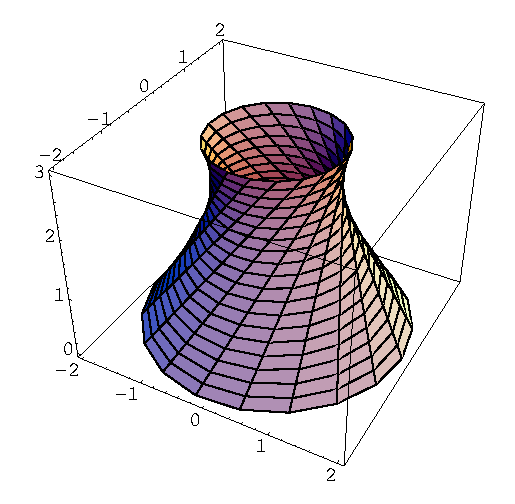
\epsfig{file=kuvat/hyperboloidi.eps}
\end{center}
\end{figure}
Pinnan kapein kohta on korkeudella $z=12/5$. \loppu

\pagebreak

\Harj
\begin{enumerate}

\item
Hahmottele seuraavien parametristen tasok�yrien kulku. Eliminoimalla parametri johda my�s
k�yr�n yht�l� karteesisessa koordinaatistossa.
\begin{align*}
&\text{a)}\ \ x=2-t,\ y=t+1,\ t\in\R \qquad\ \text{b)}\ \ x=t^2,\ y=2-t,\ t\in[0,\infty) \\
&\text{c)}\ \ x=\frac{1}{t}\,,\ y=t-1,\ t\in(0,4) \qquad\,
 \text{d)}\ \ x=\frac{1}{1+t^2}\,,\ y=\frac{t}{1+t^2}\,,\ t\in\R \\
&\text{e)}\ \ \vec r=3\sin\pi t\,\vec i+4\cos\pi t\,\vec j,\ t\in[-1,1] \\[1mm]
&\text{f)}\ \ x=1-\sqrt{4-t^2}\,,\ y=2+t,\ t\in[-2,2] \\[1mm] 
&\text{g)}\ \ \vec r=t\cos t\,\vec i+t\sin t\,\vec j,\ t\in[0,4\pi]
\end{align*}

\item
a) Tasok�yr�n er�s parametrisointi on $\vec r=\cos 2t\,\vec i+\sin^2 t\,\vec j,\ t\in\R$. 
Anna k�yr�lle vaihtoehtoinen, mahdollisimman yksinkertainen parametrisointi.
\vspace{1mm}\newline
b) Totea, ett� $\,\vec r=(t-1)\vec i+\sqrt{2t-t^2}\,\vec j,\ t\in[0,2]\,$ ja 
$\,\vec r=t\sqrt{2-t^2}\,\vec i+(1-t^2)\vec j$, \newline $t\in[-1,1]$ ovat saman k�yr�n 
parametrisointeja. Mik� k�yr� on kyseess�?

\item \index{Cartesiuksen lehti}
Tasok�yr� $S:\,x^3+y^3=3xy\,$ on nimelt��n \kor{Cartesiuksen lehti}. Johda k�yr�lle
parametriesitys kirjoittamalla $y=tx$. Hahmottele k�yr�n kulku parametrimuodosta ja merkitse
kuvioon, mitk� k�yr�n osat vastaavat parametrin arvoja v�leill� $(-\infty,-1)$, $(-1,0)$ ja 
$[0,\infty)$. Miksei $t=-1$ vastaa mit��n k�yr�n pistett�?

\item \index{venytetty sykloidi}
Ympyr�, jonka s�de on $R=1$, vierii liukumatta pitkin positiivista $x$-akselia. Ympyr�n mukana
py�rii siihen kiinnitetty jana, jonka toinen p��tepiste on ympyr�n keskipisteess� ja keskipiste
on ympyr�n keh�ll�. M��rit� janan toisen (ympyr�n ulkopuolella olevan) p��tepisteen sijainti
parametrisena k�yr�n� $x=x(t),\ y=y(t)$, miss� $t$ on ympyr�n vierimiskulma mitattuna 
alkutilanteesta, jossa janan p��tepisteet ovat $(0,1)$ ja $(0,3)$. Hahmottele k�yr�
graafisesti. Miss� pisteess� k�yr� leikkaa ensimm�isen kerran itsens�? (K�yr�� sanotaan 
\kor{venytetyksi sykloidiksi}.)

\item
Parametrisoi tason $T\,:x+y=4$ ja kartion $K:\,xy+yz+xz=0$ leikkausk�yr� ottamalla
parametriksi\, a) $t=x$, \ b) $t=x-y$.

\item
a) Avaruusk�yr�n $S$ parametrisointi on $\vec r = \vec r_0+\cos t\,\vec a+\sin t\,\vec b$,
$\,t\in[0,2\pi]$, miss� $\vec a$, $\vec b$ ja $\vec r_0$ ovat avaruusvektoreita. T�sm�lleen
mill� ehdoilla $S$ on avaruusympyr�?
\vspace{1mm}\newline
b) Avaruusympyr�n keskipiste on $(1,1,2)$, s�de on $R=3$ ja ympyr� on tasossa $x-y-3z+6=0$.
Johda ympyr�lle jokin parametrisointi muotoa $\vec r=\vec r_0+\cos t\,\vec a+\sin t\,\vec b$,
$\,t\in[0,2\pi]$.

\item
N�yt�, ett� yht�l�ryhm�
$\D \ \begin{cases} \,x^2+y+z=2 \\ \,xy+z=1 \end{cases} $ \vspace{1mm}\newline
m��rittelee kaksi leikkaavaa avaruusk�yr��, joista toisen parametrisointi on
$\vec r=t\vec i+(1+t)\vec j+(1-t-t^2)\vec k,\ t\in\R$. Millainen on toinen k�yr�?

\item \index{zzb@\nim!Kiukkulintu ja kuulanty�nt�j�t} (Kiukkulintu ja kuulanty�nt�j�t)\, 
a) Kiukkulintu lenn�tet��n alkupisteest� $(x,y)$ $=(0,1)$ (pituusyksikk� = cm) venytt�m�ll� 
heittoparaabelissa (ks.\ Esimerkki\,\ref{heittoparaabeli}) vakion $a$ arvoksi $8$ cm ja
t�ht��m�ll� porsaaseen, joka on pisteess� $(4,3)$. Mill� $k$:n arvoilla tulee
osuma? \vspace{1mm}\newline 
b) Teekkarit Yrj�l� ja St�hlberg kisaavat kuulanty�nn�ss�. Ratkaise, kumpi voitti, kun
kisaajien parhaissa ty�nn�iss� heittoparaabelin parametrit ovat \newline
Yrj�l�:   $\,\ \qquad h=2.00$ m, $\ \alpha=60.0\aste$, $\ a=8.00$ m \newline
St�hlberg: $\quad h=1.80$ m, $\ \alpha=30.0\aste$, $\ a=6.65$ m

\item
Esit� jokin parametrisointi seuraavien yht�l�iden m��r��mille pinnoille: \newline
a)\, $x^3y^2z=5,\,\ $ b)\, $(x-z)(x+z)+y+2z=0,\,\ $ c)\, $x\sin z+xy^5+y=1$

\item
a) Johda pinnalle $S$ yht�l� muotoa $F(x,y,z)=0$ parametrisoinnista
\[ 
S:\ \begin{cases}
    \,x=3+2\sin\theta\cos\varphi, \\
    \,y\,=-1+\sin\theta\sin\varphi, \\
    \,z=2+3\cos\theta, \quad (\theta,\varphi)\in\Rkaksi.
    \end{cases}
\]
b) Pallon $K$ keskipiste on $(1,1,1)$ ja s�de on $R=2$. Kuvan piirtoa varten halutaan
parametrisoida pallon $xy$-tason yl�puolinen ($z \ge 0$) osa. Esit� parametrisointi!
\vspace{1mm}\newline
c) Pinnan $S$ yht�l� lieri�koordinaateissa on $\,r=\varphi,\ (\varphi,z) \in A$, miss�
$A=[0,4\pi]\times[-5,5]$. Parametrisoi $S$ viivoitinpintana. Millainen on $S$:n ja
$xy$-tason leikkausk�yr�? \vspace{1mm}\newline
d) Pinnan yht�l� lieri�koordinaateissa on $r=z^2\abs{\cos\varphi}$. Esit� pinnan yht�l�
karteesisissa koordinaateissa. Millaisia ovat pinnan ja tasojen $z=c$ ($c\in\R$)
leikkausk�yr�t?

\item \index{hyperboloidi} \index{kaksivaippainen hyperboloidi}
a) M��rit� sen viivoitinpinnan yht�l� (muodossa $F(x,y,z)=0$), joka syntyy, kun suora
$S:\ x=z,\ y=1$ py�r�ht�� $x$-akselin ymp�ri. Totea, ett� sama pinta (nimelt��n yksivaippainen
hyperboloidi) syntyy my�s, kun er�s $xy$-tason k�yr� $K$ py�r�ht�� $x$-akselin ymp�ri. 
Hahmottele $K$ graafisesti. \vspace{1mm}\newline 
b) Tasok�yr�n $K: x^2-y^2=1$ py�r�ht�ess� $x$-akselin ymp�ri syntyy pinta nimelt�
\kor{kaksivaippainen hyperboloidi}. M��rit� ko.\ pinnan yht�l�. Miss� pisteiss� suora
$x=y=z$ leikkaa pinnan?

\item
a) Puolikartion $K$ k�rki on origossa, symmetria-akseli on positiivinen $z$-akseli ja
puolisuora $x=2y=3z,\ x \ge 0$ on pinnalla $K$. Parametrisoi $K$ py�r�hdyspintana ja
viivoitinpintana. Mik� on $K$:n yht�l� lieri�koordinaatistossa? \vspace{1mm}\newline
b) Parametrisoi kartio $K:\ xy+yz+xz=0\,$ viivoitinpintana.

\item (*) \index{asteroidi} \index{hyposykloidi}
Ympyr�n keskipiste on origossa ja s�de on $a$. Ympyr�� pitkin sen sis�puolella vierii liukumatta
toinen ympyr�, jonka s�de on $b<a$. T�ll�in vieriv�n ympyr�n kiinte� piste $P$ piirt�� 
tasok�yr�n nimelt� \kor{hyposykloidi}. \ a) N�yt�, ett� pisteen $(a,0)$ kautta kulkevan
hyposykloidin parametriesitys on
\[
x=(a-b)\cos t+b\cos\left(\frac{a-b}{b}\,t\right), \quad
y=(a-b)\sin t-b\sin\left(\frac{a-b}{b}\,t\right).
\]
b) P��ttele, ett� tapauksessa $a=2b$ piste $P$ liikkuu pitkin janaa. \newline
c) N�yt�, ett� tapauksessa $a=4b$ parametriesitys yksinkertaistuu muotoon 
\[
x=a\cos^3 t,\ \ y=a\sin^3 t.
\] 
Hahmottele t�m�n k�yr�n --- nimelt��n \kor{asteroidi} --- kulku. Mik� on asteroidin yht�l�
karteesisissa koordinaateissa? 

\item (*) \index{zzb@\nim!Sotaharjoitus 1}
(Sotaharjoitus 1) Origosta ammutun tykinkuulan lentorata on ajan $t$ funktiona (yksik�t km ja s)
\[ \begin{cases}
x(t)=(\sin\theta\cos\varphi+a)\,t, \\
y(t)=(\sin\theta\sin\varphi+b)\,t, \\
z(t)=(\cos\theta)\,t-0.005\,t^2,
\end{cases} \]
miss� $\theta,\varphi$ ovat suuntauskulmat ja $a,b$ ovat tuuliparametreja. Maastoesteet
asettavat suuntaukselle rajoituksen $\tan\theta > 0.2$. Miten suuntaus on valittava 
tuulettomassa s��ss� ($a=b=0$), jotta ammus osuisi pisteess� $(10,20,0)$ olevaan maaliin? 
Kuinka korkealla ammus k�y? Kuinka kauas maalista ammus osuu t�ll� suuntauksella, jos 
$a=0.002$ ja $b=-0.001$\,? %Miten suuntausta olisi (likimain) muutettava?

\item (*)
Jana, jonka pituus on $20$, liikkuu seuraavasti: Janan keskipiste liikkuu $z$-akselia pitkin
positiiviseen suuntaan vakionopeudella. Liikkuessaan jana pysyy $xy$-tason suuntaisena ja py�rii
tasaisesti (kulmanopeus vakio) siten, ett� keskipisteen liikkuessa $30$ pituusyksikk��
jana py�rii t�yden kierroksen positiivisen $z$-akselin suunnasta katsottuna vastap�iv��n.
Esit� janan avaruuteen piirt�m�n viivoitinpinnan $S$ parametrisointi, kun tiedet��n lis�ksi,
ett� piste $(1,0,0)$ on t�ll� pinnalla. Leikkaako suora $z=25,\ x+y=4$ pinnan $S$\,?

\end{enumerate} %yhdistetty vanhat IV-5 ja IV-6, poistokamaa -> IV-5a
\include{IV-5}
\chapter{Jatkuvuus ja derivoituvuus}  \label{jatkuvat funktiot}

Funktion \kor{jatkuvuus} ja \kor{derivoituvuus} ovat k�sitteellisi� perusl�ht�kohtia 
matematiikan suuntauksessa, jota kutsutaan v�lj�sti \kor{analyysiksi}. Jatkuvuudesta, tai 
yleisemmin funktion \kor{s��nn�llisyydest�} puhuttaessa on kyse funktion arvojen
ennustettavuudesta muuttujan (muuttujien) arvojen vaihdellessa. Jatkuvuuden ja derivoituvuuden
k�sitteet tuovat matemaattisten funktioiden teoriaan kokonaan oman 'makunsa' verrattuna
t�h�n asti tarkasteltuun funktioiden algebraan.

T�ss� luvussa tarkastelun kohteena ovat p��osin vain yhden reaalimuuttujan funktiot. N�ille
funktioille m��ritell��n ensin jatkuvuus perusk�sitteen� ja jatkuvuuteen l�heisesti liittyv�
\kor{funktion raja-arvon} k�site. Pelkk�� jatkuvuutta vahvempina s��nn�llisyyden lajeina
m��ritell��n mm.\ derivoituvuus (Luku \ref{derivaatta}) ja derivoituvuutta vahvemmat 
\kor{sileyden} lajit (Luku \ref{��riarvot}). N�iden k�sitteiden pohjalta luonnehditaan
funktioita, mm.\ esitet��n kaksi reaalimuuttujan analyysin keskeist� \kor{v�liarvolausetta} ja
tarkastellaan n�iden lauseiden seuraamuksia yht�l�iden ja my�s yksinkertaisten 
\kor{differentiaaliyht�l�iden} ratkeavuusteoriassa. 

Derivaatta tuo mukanaan my�s derivoimiss��nn�t eli uuden ulottuvuuden funktioalgebraan.
Luvuissa \ref{derivaatta}--\ref{kaarenpituus} johdetaan kaikki keskeiset derivoimiss��nn�t,
mukaanlukien implisiittifunktiot, potenssisarjan summana m��ritellyt funktiot ja
(Luvussa \ref{kaarenpituus} erikseen) trigonometriset funktiot. 

Luvussa \ref{kiintopisteiteraatio} tarkastelun kohteena ovat yht�l�itten likim��r�isess�
ratkaisussa yleisesti k�ytett�vien algoritmien, \kor{kiintopisteiteraatioiden},
toimintaperiaatteet ja suppenevuusteoria. Luvussa \ref{analyyttiset funktiot} tarkastellaan
lyhyesti jatkuvuuden ja derivoituvuuden k�sitteiden laajentamista kompleksifunktioihin ja
m��ritell��n t�h�n liittyen \kor{analyyttisen} kompleksifunktion k�site. Viimeisess�
osaluvussa todistetaan jatkuvien funktioiden teorian keskeisimpi� v�itt�mi� kuten 
\kor{Weierstrassin lause}. T�ss� yhteydess� esitet��n my�s lyhyesti, miten Algebran peruslause
on todistettavissa kompleksialgebran ja analyysin tuloksia yhdistelem�ll�.

\section{Jatkuvuuden käsite} \label{jatkuvuuden käsite}
\alku

Funktion jatkuvuuden ongelma tulee eteen niinkin yksinkertaisessa tehtävässä kuin funktion
arvon numeerisessa määrittämisessä, eli numeerisessa funktioevaluaatiossa. Tarkastellaan Luvun 
\ref{käänteisfunktio} Esimerkin \ref{algebrallinen käänteisfunktio} käänteisfunktiota, 
joka nyt kirjoitettakoon muotoon
\[
y=f(x) \ \ekv \ y^5+3y=x, \quad x\in\R.
\]
Tehtävänä olkoon laskea likimäärin luku $a=f(\pi)$, eli evaluoida $f$ numeerisesti $\pi$:ssä. 
Tähän itse asiassa sisältyy kaksi numeerista ongelmaa: Ensinnäkin luvulle $\pi$ ei ole olemassa
'tarkkaa' numeerista arvoa, ja toiseksi yhtälöä ei yleensä voi ratkaista $y$:n suhteen
tarkasti, vaikka $x$ olisi rationaaliluku. Käytännössä menetellään (laskin/tietokone 
menettelee) seuraavasti: Valitaan $\pi$:lle edustaja $x_n$ rationaalilukujonosta $\{x_n\}$,
jolle pätee $x_n\rightarrow \pi$. Lasketaan $a_n=f(x_n)$ likimäärin käyttämällä jotakin
numeerista algoritmia yhtälön $y^5+y=x_n$ ratkaisuun. Algoritmi tuottaa käytännössä
rationaalilukujonon $\{b_k\}$, jolle pätee $b_k \kohti a_n$ kun $k\rightarrow\infty$. Poimitaan
tästä jonosta luvun $a_n$ likiarvoksi $b_m$ jollakin $m$ (esim.\ $m=10$), ja ilmoitetaan
lopputuloksena tämän luvun likiarvo äärellisenä desimaalilukuna (katkaistuna tai pyöristettynä
liukulukuna). 

Jos em.\ laskussa ei huomioida numeerisia pyöristysvirheitä liukulukulaskennassa, niin 
lopputuloksen $b_m$ virhe koostuu kahdesta osasta:
\[
b_m-f(\pi)\,=\,[b_m-f(x_n)]+[f(x_n)-f(\pi)].
\]
Tässä ensimmäinen osa on approksimaation $b_m \approx f(x_n)$ virhe, eli kyse on yhtälön
$y^5+3y=x_n$ ratkaisualgoritmin tarkkuudesta. Virheen jälkimmäisessä osassa sen sijaan on kyse,
paitsi approksimaation $x_n \approx x$ tarkkuudesta, myös funktiosta $f$: Kyse on funktion 
j\pain{atkuvuudesta}. Kvalitatiivisesti väittämä '$f$ on jatkuva $x$:ssä' tarkoittaa, että
funktioevaluaatio $x \map f(x)$ on luotettava, kun muuttujalle sallitaan pieni vaihtelu, ts.\
pätee
\[
x_n\approx x \ \impl \ f(x_n)\approx f(x).
\]

Em.\ funktion tapauksessa jatkuvuuskysymys ratkeaa seuraavasti: Koska
\[
\begin{cases}
a^5+a=\pi, \\
a_n^5+a_n=x_n,
\end{cases}
\]
saadaan vähennyslaskulla (vrt. Luvun \ref{käänteisfunktio} tarkastelut)
\[
(a-a_n)(a^4+a^3a_n+a^2a_n^2+aa_n^3+a_n^4+3)=\pi-x_n.
\]
Tässä voidaan turvallisesti olettaa, että $a,a_n \ge 0$, joten seuraa
\[
\abs{a_n-a}\le \tfrac{1}{3}\abs{x_n-\pi}\,\ \ekv\,\ 
\abs{f(x_n)-f(\pi)}\le\tfrac{1}{3}\abs{x_n-\pi}.
\]
Jatkuvuudelle on näin saatu jopa kvantitatiivinen varmistus: Approksimaation $f(x_n)$ $\approx$
$f(\pi)$ virhe on enintään kolmasosa approksimaation $x_n\approx \pi$ virheestä. 

Esimerkki johdattaa seuraavaan funktion jatkuvuuden määritelmään (vaihtoehtoinen määritelmä 
jäljempänä).
\begin{Def} \vahv{(Jatkuvuus: jonokriteeri)}\ \label{funktion jatkuvuus}
\index{jatkuvuus (yhden muuttujan)|emph} \index{epzy@epäjatkuvuus (funktion)|emph}
Funktio $f:\DF_f\rightarrow\R,\ \DF_f\subset\R$, on \kor{jatkuva} (engl.\ continuous, ruots.\ 
kontinuerlig) \kor{pisteessä} $a\in\DF_f$ (tai $a$:ssa), jos kaikille reaalilukujonoille
$\seq{x_n}$ pätee
\[
x_n\in\DF_f\ \forall n\,\ \ja\,\ x_n \kohti a\,\ \impl\,\ f(x_n) \kohti f(a).
\]
Jos $f$ ei ole jatkuva pisteessä $a\in\DF_f$, niin $f$ on \kor{epäjatkuva}
(engl.\ discontinuous) pisteesä $a$.
\end{Def}
\begin{Exa} \label{epäjatkuva funktio} Funktio \
$\D f(x)= \begin{cases} \,x-1, &\text{jos}\ x<\pi \\ \,x, &\text{jos}\ x\ge\pi \end{cases}$
\vspace{1mm}\newline
on epäjatkuva pisteessä $x=\pi$, sillä jos $x_n \kohti \pi$ ja $x_n<\pi\ \forall n$, niin
$f(x_n)=x_n-1 \kohti \pi-1 \neq f(\pi)=\pi$. Muissa pisteissä $f$ on jatkuva, sillä jos esim.\
$a<\pi$ ja $x_n \kohti a$, niin jostakin indeksistä $N$ eteenpäin on $\abs{x_n-a}<\pi-a$ 
(lukujonon suppenemisen määritelmässä valittu $\eps=\pi-a$), jolloin on erityisesti 
$x_n-a < \pi-a\ \ekv\ x_n<\pi$, kun $n>N$. Tällöin on $f(x_n)=x_n-1,\ n>N$ ja siis
$f(x_n) \kohti a-1=f(a)$. \loppu
\end{Exa}
\begin{Exa} Olkoon $\DF_f=\{a\}$ ($a\in\R$) ja $f(a)=c\in\R$. Määritelmän
\ref{funktion jatkuvuus} mukaisesti $f$ on jatkuva pisteessä $a$\,(!). Yleisemmin
reaalifunktio on jatkuva jokaisessa määrittelyjoukkonsa nk.\ \kor{eristetyssä pisteessä},
ks.\ Harj.teht.\,\ref{H-V-1: eristetty piste}. \loppu
\end{Exa}
Jatkuvuus voidaan määritellä myös suoraan vetoamatta lukujonoihin, jolloin määritelmästä tulee 
lukujonon suppenemisen määritelmää (Määritelmä \ref{jonon raja}) muistuttava. Vaihtoehtoinen
määritelmä on seuraava.
\begin{Def} \vahv{(Jatkuvuus: $(\eps,\delta)$-kriteeri)}\ \label{vaihtoehtoinen jatkuvuus}
\index{jatkuvuus (yhden muuttujan)|emph}
Funktio $f:\DF_f\kohti\R,\ \DF_f\subset\R$, on jatkuva pisteessä $a\in\DF_f$, jos jokaisella
$\eps>0$ on olemassa $\delta>0$ siten, että jokaisella $x\in\R$ pätee
\[
x\in\DF_f\,\ \ja\,\ \abs{x-a}<\delta\,\ \impl\,\ \abs{f(x)-f(a)}<\eps.
\]
\end{Def}
Määritelmiä \ref{funktion jatkuvuus} ja \ref{vaihtoehtoinen jatkuvuus} verrattaessa ei näytä
aivan ilmeiseltä, että pätee (ks.\ todistus luvun lopussa)
\begin{*Lause} \label{jatkuvuuskriteerien yhtäpitävyys} Jatkuvuuden määritelmät
\ref{funktion jatkuvuus} ja \ref{vaihtoehtoinen jatkuvuus} ovat yhtäpitävät.
\end{*Lause} 
\jatko\jatko \begin{Exa} (jatko) Jos $a\neq\pi$, niin esimerkin funktiolle pätee
\[
\abs{f(x)-f(a)}=\abs{x-a}, \quad \text{kun}\ \abs{x-a}<\abs{\pi-a},
\]
joten Määritelmän \ref{vaihtoehtoinen jatkuvuus} ehto on voimassa, kun valitaan
$\delta=\min\{\eps,\abs{\pi-a}\}>0$. Siis $f$ on jatkuva pisteissä $a\neq\pi$ Määritelmän
\ref{vaihtoehtoinen jatkuvuus} mukaisesti. \loppu
\end{Exa} \seur
\begin{Exa} Näytä, että $f(x)=x^2$ on jatkuva jokaisessa pisteessä $a\in\R$
käyttäen jatkuvuuden a) jonokriteeriä,\, b) $(\eps,\delta)$-kriteeiä.
\end{Exa}
\ratk \ a) Määritelmän \ref{funktion jatkuvuus} mukainen jatkuvuus on seuraus Lauseesta
\ref{raja-arvojen yhdistelysäännöt}:
\[
x_n \kohti a \qimpl x_n^2 \kohti a^2\,\ \impl\,\ f(x_n) \kohti f(a).
\]
b) Jos $a\in\R$ ja $\abs{x-a} \le 1$, niin kunta-algebran ja kolmioepäyhtälön nojalla
\begin{align*}
\abs{f(x)-f(a)}\,=\,\abs{x-a}\abs{x+a}\,
                &=\,\abs{x-a}\abs{2a+(x-a)} \\
                &\le\,\abs{x-a}(2\abs{a}+\abs{x-a})\,
                 \le\,\abs{x-a}(2\abs{a}+1).
\end{align*}
Näin ollen jos $\eps>0$, niin pätee $\abs{f(x)-f(a)}<\eps$ aina kun
$\abs{x-a}<\delta=\min\{1,\eps/(2\abs{a}+1)\}$ (jolloin myös $\abs{x-a}<1$). Koska tässä on
$\delta>0$ aina kun $\eps>0$, niin $f$ on jatkuva $a$:ssa
Määritelmän \ref{vaihtoehtoinen jatkuvuus} mukaisesti. \loppu

Jatkuvuuden määrittely jonokriteerillä (Määritelmä \ref{funktion jatkuvuus}) on kätevää
monissa teoreettisissa tarkasteluissa, jotka tällä tavoin palautuvat suppenevien
lukujonojen teoriaan. (Tämä teoria on kylläkin tunnettava, mitä voi pitää myös
haittapuolena.) Määritelmä \ref{vaihtoehtoinen jatkuvuus} on jatkuvuuden perinteisempi
'koulumääritelmä'. Tämä on usein Määritelmää \ref{funktion jatkuvuus} selkeämpi silloin kun
halutaan selvittää, miltä jatkuvat funktiot 'näyttävät'. Esimerkiksi seuraava usein käytetty
tulos, joka kertoo jatkuvan funktion 'jäykkyydestä', on tästä määritelmästä helppo johtaa.
Todistus jätetään harjoitustehtäväksi (Harj.teht.\,\ref{H-V-1: todistuksia}a).
\begin{Prop} \label{jatkuvan funktion jäykkyys} Jos $f$ on jatkuva pisteessä $a$ ja $f(a)>0$
($f(a)<0$), niin $\exists\delta>0$ siten, että $f(x)>0$ ($f(x)<0$) aina kun 
$x\in(a-\delta,a+\delta) \cap \DF_f\,$.
\end{Prop}

Jatkuvuus yksittäisessä pisteessä voidaan laajentaa koskemaan joukkoa $A\subset\DF_f$\,:
Funktio on jatkuva $A$:ssa, jos se on jatkuva $A$:n jokaisessa pisteessä. 
Jatkuvuustarkasteluille on kuitenkin tyypillistä, että tarkastelu rajoittuu \pain{välille} 
$A\subset\DF_f$ siten, että funktion ominaisuuksilla välin ulkopuolella ei ole lainkaan
merkitystä. Sen vuoksi on tapana asettaa mainitusta yleisestä säännöstä hieman poikkeava
\begin{Def} (\vahv{Jatkuvuus välillä}) \label{jatkuvuus välillä}
\index{jatkuvuus (yhden muuttujan)!a@välillä|vahv}
Funktio $f:\DF_f\kohti\R,\ \DF_f\subset\R$, on \kor{jatkuva välillä} $A\subset\DF_f$, jos
jokaisella $x \in A$ ja jokaiselle reaalilukujonolle $\seq{x_n}$ pätee
\[
x_n \in A\ \ja\ x_n \kohti x\,\ \impl\,\ f(x_n) \kohti f(x).
\]
\end{Def}
Tämän mukaisesti jatkuvuus välillä $A$ tarkoittaa samaa kuin Määritelmän
\ref{funktion jatkuvuus} mukainen jatkuvuus $A$:n jokaisessa pisteessä siinä tapauksessa, että
funktion määrittelyjoukko rajataan väliksi $A$. (Jatkuvuuden vaihtoehtoisessa määritelmässä
\ref{vaihtoehtoinen jatkuvuus} korvataan ehto $\,x\in\DF_f\,$ ehdolla $x\in\DF_f \cap A$.)
Jatkuvuus välillä määritellään siis jatkuvuutena 'sisältä päin' ko.\ joukossa. Jos väli on
avoin, ei tämä rajaus ole tarpeen, sillä jos $x\in(a,b)=A$ ja $x_n \kohti x$, niin jollakin $N$
pätee $x_n \in A\ \forall n>N$ (Määritelmä \ref{jonon raja}, $\eps=\min\{x-a,b-x\}>0$) eli
määritelmän ehto toteutuu indeksistä $N$ eteenpäin joka tapauksessa. Sen sijaan jos väli on
suljettu, on ehdolla $x_n \in A$ merkitystä välin päätepisteissä (ei sisäpisteissä).
\jatko\jatko \jatko \begin{Exa} (jatko) Jos $b>\pi$, on esimerkin funktio $f$ jatkuva välillä
$[\pi,b]$ (Määritelmä \ref{jatkuvuus välillä}) vaikka $f$ ei ole jatkuva pisteessä $\pi$
(Määritelmä \ref{funktion jatkuvuus}). Jos $a<\pi$, on $f$ jatkuva välillä $[a,\pi)$ mutta ei
välillä $(a,\pi]$. \loppu
\end{Exa} \seur\seur
\begin{Exa} \label{Dirichlet'n funktio} \index{Dirichleta@Dirichlet'n funktio}
Funktio $\D
f(x)=\begin{cases}
     \,1, \ &\text{ jos } x\in\Q,  \\
     \,0, &\text{ jos } x\in\R, \ x\notin\Q
     \end{cases}$ \vspace{2mm}\newline
on esimerkki 'patologisesta' funktiosta, joka on määritelty koko $\R$:ssä, mutta joka ei ole 
missään pisteessä jatkuva. Funktion nimi on \kor{Dirichlet'n funktio}.  \loppu
\end{Exa}

\subsection*{Jatkuvien funktioiden yhdistely}

Esimerkin \ref{Dirichlet'n funktio} vastapainoksi voidaan kysyä, millaiset 'normaalit' funktiot 
tyypillisesti ovat jatkuvia. Ensimmäinen tuntuma näihin saadaan yhdistelemällä yksinkertaisia 
funktioita peruslaskutoimituksilla Määritelmän \ref{funktioiden yhdistelysäännöt} mukaisesti.
Koska funktion jatkuvuudessa on viime kädessä kyse lukujonon $\seq{f(x_n)}$ suppenemisesta,
on seuraava lause välitön seuraus Lauseesta \ref{raja-arvojen yhdistelysäännöt}
(Harj.teht.\,\ref{H-V-1: todistuksia}b).
\begin{Lause} (\vahv{Jatkuvuuden yhdistelysäännöt}) \label{jatkuvuuden yhdistelysäännöt}
\index{jatkuvuus (yhden muuttujan)!b@yhdistelysäännöt|emph}
Jos $f:\DF_f\kohti\R$ on jatkuva pisteessä $x\in\DF_f$, niin $\lambda f$ on jatkuva $x$:ssä 
$\forall\lambda\in\R$. Jos lisäksi $x\in\DF_g$ ja $g:\DF_g\kohti\R$ on jatkuva pisteessä $x$,
niin $f+g$ ja $fg$ ovat jatkuvia $x$:ssä. Jos edelleen $g(x)\neq 0$, niin myös $f/g$ on
jatkuva $x$:ssä.
\end{Lause}
\begin{Exa} Jokainen polynomi tai rationaalifunktio voidaan määritellä palautuvasti
algebrallisena yhdistelmänä perusfunktioista $f_0(x)=1$ ja $f_1(x)=x$. Koska nämä ovat
ilmeisen jatkuvia $\R$:ssä, niin päätellään Lauseesta \ref{jatkuvuuden yhdistelysäännöt},
että jokainen polynomi on jatkuva $\R$:ssä ja jokainen rationaalifunktio
määrittelyjoukossaan, eli muualla kuin nimittäjänsä nollakohdissa. \loppu 
\end{Exa}
\begin{Exa} \label{trig yhdistely} Jos pidetään tunnettuna, että trigonometriset funktiot
$\sin$ ja $\cos$ ovat jatkuvia $\R$:ssä, niin Lauseen \ref{jatkuvuuden yhdistelysäännöt}
perusteella funktiot $\tan=\sin/\cos$ ja $\cot=\cos/\sin$ ovat samoin jatkuvia koko
määrittelyjoukossaan. \loppu 
\end{Exa}
\begin{Lause} (\vahv{Yhdistetyn funktion jatkuvuus}) \label{yhdistetyn funktion jatkuvuus}
\index{jatkuvuus (yhden muuttujan)!c@yhdistetyn funktion|emph}
Jos $g$ on jatkuva pisteessä $x\in\DF_g$, $g(x)\in\DF_f$ ja $f$ on jatkuva pisteessä $g(x)$,
niin yhdistetty funktio $f\circ g$ on jatkuva $x$:ssä.
\end{Lause}
\tod Koska $\,x_n\in\DF_{f \circ g}\ \ekv\ x_n\in\DF_g\,\wedge\,g(x_n)\in\DF_f$, niin
jonokriteerin avulla päätellään:
\begin{align*}
x_n \in\DF_{f\circ g}\ \ja\ x_n \kohti x 
           &\qimpl g(x_n)\in\DF_f\ \ja\ x_n\in\DF_g\ \ja\ x_n \kohti x \\
           &\qimpl g(x_n)\in\DF_f\ \ja\ g(x_n) \kohti g(x) \\
           &\qimpl f(g(x_n)) \kohti f(g(x)). \quad\loppu
\end{align*}
\begin{Exa} \label{itseisarvon jatkuvuus} Näytä, että jos $f$ on jatkuva $x$:ssä, niin myös
$\abs{f}$ on jatkuva $x$:ssä. 
\end{Exa}
\ratk Funktio $g(x)=\abs{x}$ on helposti osoitettavissa jatkuvaksi $\R$:ssä suoraan
jatkuvuuden määritelmistä (tai vedoten Propositioon \ref{jatkuvuuspropositio} alla), joten
Lauseen \ref{yhdistetyn funktion jatkuvuus} nojalla yhdistetty funktio 
$(g \circ f)(x) = \abs{f(x)}$ on jatkuva jokaisessa pisteessä, jossa $f$ on jatkuva. \loppu

Jatkuvuuden periytyvyyden p\pain{aloittain} (eli eri väleillä erilaisilla laskusäännöillä)
määritellyn funktion osalta ratkaisee
(Harj.teht.\,\ref{H-V-1: todistuksia}c; vrt.\ myös Esimerkki \ref{epäjatkuva funktio} edellä).
\begin{Prop} \label{jatkuvuuspropositio}
Olkoon $f_1$ ja $f_2$ jatkuvia avoimella välillä $(a,b)$ ja
\[
f(x) = \begin{cases} 
       \,f_1(x), &\text{kun}\ x \in (a,c), \\ 
       \,k, &\text{kun}\ x=c, \\ 
       \,f_2(x), &\text{kun}\ x \in (c,b),
       \end{cases} 
\]
missä $a<c<b$. Tällöin $f$ on jatkuva $c$:ssä täsmälleen kun $\,f_1(c)=f_2(c)=k$. 
\end{Prop}
\begin{Exa} Funktio
\[ f(x) = \begin{cases}
          \ x+a,\ &\text{kun}\ x \le a, \\ -(x+1)^2,\ &\text{kun}\ x > a 
          \end{cases} 
\] 
on polynomi $f_1(x)=x+a$ välillä $(-\infty,a)$ ja polynomi $f_2(x)=-(x+1)^2$ välillä
$(a,\infty)$, joten näillä väleillä funktio on jatkuva. Proposition \ref{jatkuvuuspropositio}
mukaan ehto funktion jatkuvuudelle pisteessä $x=a$ (ja siis ehto jatkuvuudelle koko $\R$:ssä)
on
\[
f_1(a)=f_2(a) \qekv a^2+4a+1=0 \qekv a = -2 \pm \sqrt{3}. \loppu
\]
\end{Exa}

\subsection*{Funktio $f(x) = \sqrt[m]{x}$}
\index{jatkuvuus (yhden muuttujan)!d@funktion $\sqrt[m]{x}$|vahv}

Osoitetaan seuraavaksi, että funktio $f:[0,\infty)\rightarrow [0,\infty)$, joka määritellään
\[
f(x)=x^{1/m}=\sqrt[m]{x},\quad m\in\N, \ m\geq 2
\]
on koko määrittelyvälillään jatkuva (kuvassa $f(x)$, kun $m=8$).
\begin{figure}[H]
\begin{center}
\epsfig{file=plots/8throotx.eps}
%\caption{$y=\sqrt[8]{x}$}
\end{center}
\end{figure}
Aloitetaan pisteestä $x=0$, joka on jatkuvuuden kannalta kriittisin (vrt. kuva). Koska f on 
aidosti kasvava (ks.\ Luku \ref{käänteisfunktio}, Esimerkki \ref{x^m:n käänteisfunktio}),
niin jokaisella $a>0$ pätee
\[
0 \le x < a^m\ \ekv\ 0 \le f(x) < f(a^m) = a.
\]
Jos nyt $x_n\geq 0$ ja $x_n\rightarrow 0$, niin jokaisella $\eps>0$ $\exists N\in\N$ siten,
että pätee
\[
n>N \ \impl \ 0 \le x_n < \eps^m \ \impl\ 0 \le f(x_n) < \eps.
\]
Näin ollen lukujono $\{f(x_n)\}$ on suppeneva ja $f(x_n) \kohti 0=f(0)$, joten $f$ on jatkuva 
$0$:ssa.

Muualla kuin origossa $f$:n jatkuvuus voidaan päätellä kunta-algebran avulla: Jos 
$x_n \ge 0$ ja $x_n \kohti x>0$, niin merkitsemällä $y=f(x)$, $y_n=f(x_n)$ seuraa
\[
x-x_n \,=\, y^m-y_n^m \,=\, (y-y_n)(y^{m-1}+y^{m-1}y_n+\cdots +y_n^{m-1}).
\]
Tässä on $y_n \ge 0$, $y>0$, joten päätellään
\[
\abs{x-x_n}\,\ge\,\abs{y-y_n}y^{m-1} \,\ \ekv\,\ \abs{y-y_n}\,\le\,y^{1-m}\abs{x-x_n}.
\]
Näin ollen $x_n \kohti x \ \impl\ y_n \kohti y$, eli $f$ on jatkuva pisteessä $x$.
\begin{Exa} \label{epsilon ja delta} Olkoon $\eps = 10^{-6}$. Määritä suurin $\delta$ siten,
että Määritelmän \ref{vaihtoehtoinen jatkuvuus} ehto toteutuu funktiolle $f(x)=\sqrt[8]{x}$
pisteessä $x=0$.
\end{Exa}
\ratk Koska $f$ on aidosti kasvava välillä $[0,\infty)=\DF_f$, niin $\forall x\in\DF_f$ pätee
$|f(x)-f(0)|=\sqrt[8]{x} < \eps\ \ekv\ 0 \le x < \eps^8\ \ekv\ x\in(-\eps^8,\eps^8)\cap\DF_f$.
Siis $\,\delta_{max} = \eps^8 = 10^{-48}$. \loppu

Funktion $f(x)=x^{1/m}$ jatkuvuuden tultua todetuksi seuraa Lauseesta 
\ref{yhdistetyn funktion jatkuvuus} ja funktion $g(x)=\abs{x}$ jatkuvuudesta, että yhdistetty 
funktio $(f\circ g)(x) = \abs{x}^{1/m}$ on jatkuva koko määrittelyjoukossaan ($= \R$). Kun
huomioidaan myös Lause \ref{jatkuvuuden yhdistelysäännöt}, niin seuraa
\begin{Prop} \label{potenssifunktion jatkuvuus}
Funktio $f(x)=\abs{x}^\alpha$, $\alpha=p/q\in\Q$ on koko määrittelyjoukossaan ($\DF_f=\R$ jos
$\alpha>0$, $\DF_f=\{x\in\R \mid x \neq 0\}$ jos $\alpha \leq 0$) jatkuva.
\end{Prop}
Lauseiden \ref{jatkuvuuden yhdistelysäännöt}--\ref{yhdistetyn funktion jatkuvuus}, Proposition
\ref{potenssifunktion jatkuvuus} ja Esimerkkien \ref{trig yhdistely} ja
\ref{itseisarvon jatkuvuus} perusteella voidaan vetää se yleisempi johtopäätös, että kaikki
toistaiseksi tunnetut 'yhden lausekkeen' funktiot ovat jatkuvia koko määrittelyjoukossaan (!).
\begin{Exa} Ilman tapauskohtaista tarkastelua voidaan esimerkiksi seuraavat funktiot
päätellä jatkuviksi määrittelyjoukkonsa jokaisessa pisteessä:
\[
\sqrt[3]{\abs{1-\sqrt{x}\,}}\,, \quad 
\sqrt[6]{\frac{1+\sqrt{x}}{2-x^2}}\,, \quad
\frac{|\sin x|^{3/4}}{x-\pi}\,, \quad 
\frac{\cot x}{\sqrt[4]{x+50\cos(\tan x)}}\,. \loppu
\]
\end{Exa}

\subsection*{Jatkuvien funktioiden päälauseet}

Tässä osaluvussa esitetään kolme matemaattisen analyysin keskeistä lausetta, jotka kaikki
koskevat suljetulla välillä jatkuvia funktioita. Ensimmäinen lauseista on myös ensimmäinen
yhden reaalimuuttujan funktioita koskevista \kor{väliarvolauseista}, joita on kaikkiaan kolme.
(Muut kaksi esitetään myöhemmin.) Tässä esitettävistä päälauseista jälkimmäiset kaksi ovat
erikoistapauksia yleisemmistä väittämistä, jotka perustuvat jatkuvuuden syvällisempään
logiikkaan. Näiden todistuksia ei vielä esitetä, vaan lauseet muotoillaan ja todistetaan
jäljempänä Luvussa \ref{jatkuvuuden logiikka} tässä esitettyä yleisemmässä muodossa. 
 
Tarkastellaan suljetulla välillä $[a,b]$ jatkuvaa funktiota $f$. Olkoon $f(a) \neq f(b)$ ja 
$c < \eta < d$, missä
\[ 
c = \min \{f(a),f(b)\}, \quad d = \max\{f(a),f(b)\}. 
\]
Koska $f$ on jatkuva, niin tuntuu luonnolliselta ajatella, että $f$:n kuvaaja välillä $[a,b]$
on 'jatkuva lanka', joka yhdistää pisteet $A=(a,f(a))$ ja $B=(b,f(b))$. Tämän intuition
mukaisesti tuntuu selvältä, että kuvaajan on leikattava suora $y=\eta$ ainakin kerran välillä
$(a,b)$. Toisin sanoen, probleemalla
\[ 
x \in [a,b]: \quad f(x) = \eta 
\]
on oltava ainakin yksi ratkaisu $x=\xi \in (a,b)$ jokaisella $\eta \in (c,d)$ (kuva).
\begin{figure}[H]
\setlength{\unitlength}{1cm}
\begin{center}
\begin{picture}(10,6)(-1,-1)
\put(-1,0){\vector(1,0){10}} \put(8.8,-0.4){$x$}
\put(0,-1){\vector(0,1){6}} \put(0.2,4.8){$y$}
\curve(
    1.0000,    1.0000,
    1.5000,    2.7969,
    2.0000,    3.4643,
    2.5000,    3.4174,
    3.0000,    3.0000,
    3.5000,    2.4844,
    4.0000,    2.0714,
    4.5000,    1.8906,
    5.0000,    2.0000,
    5.5000,    2.3862,
    6.0000,    2.9643,
    6.5000,    3.5781,
    7.0000,    4.0000,
    7.5000,    3.9308,
    8.0000,    3.0000)
\put(0.9,0.9){$\bullet$} \put(0.5,0.6){$A$}
\put(7.9,2.9){$\bullet$} \put(8.2,3.1){$B$}
\dashline{0.2}(5.5,0)(5.5,2.39)(0,2.39)
\dashline{0.05}(1,0)(1,1)(0,1)
\dashline{0.05}(8,0)(8,3)(0,3)
\put(0.9,-0.5){$a$} \put(5.4,-0.5){$\xi$} \put(7.9,-0.5){$b$}
\put(-0.4,0.9){$c$} \put(-0.4,2.3){$\eta$} \put(-0.4,2.9){$d$}
\end{picture}
%\caption{Väliarvolauseen väittämän havainnollistaminen}
\end{center}
\end{figure}
Ym.\ geometriselle intuitiolle vahvistuksen antaa
%\begin{figure}[H]
%\setlength{\unitlength}{1mm}
%\begin{center}
%\begin{picture}(140,45)(0,10)
%\put(20,20){\vector(1,0){40}} \put(58,16){$x$}
%\put(20,20){\vector(0,1){30}} \put(22,48){$y$}
%\put(80,20){\vector(1,0){40}} \put(118,16){$x$}
%\put(80,20){\vector(0,1){30}} \put(82,48){$y$} 
%\curve(25,25,45,32,55,45)
%%\curve(85,45,95,32,115,25)
%%\curve(25,15,45,50,55,45)
%\curve(85,55,95,20,115,32)
%\dashline{1}[0.2](30,20)(30,26)(20,26)
%\dashline{1}[0.2](53,20)(53,41)(20,41)
%\dashline{1}[0.2](87,20)(87,40)(80,40)
%\dashline{1}[0.2](110,20)(110,26)(80,26)
%\put(29,16){$a$} \put(16,25){$c$} \put(52,16){$b$} \put(16,40){$d$}
%\put(86,16){$a$} \put(76,39){$c$} \put(109,16){$b$} \put(76,25){$d$}
%\end{picture}
%\end{center}
%\end{figure}
\begin{Lause} \label{ensimmäinen väliarvolause}
\vahv{(Ensimmäinen väliarvolause --- Jatkuvien funktioiden väliarvolause)}
\index{vzy@väliarvolauseet!a@jatkuvien funktioiden|emph}
Jos $f:\DF_f\kohti\R$, $\DF_f\subset\R$, on jatkuva välillä $[a,b]\subset\DF_f$ ja 
$c=\min\{f(a),f(b)\}<d=\max\{f(a),f(b)\}$ (eli $f(a) \neq f(b)$), niin jokaisella 
$\eta\in (c,d)$ on olemassa $\xi \in (a,b)$ siten, että $f(\xi)=\eta$.\footnote[2]{Lause
\ref{ensimmäinen väliarvolause} varmistaa, että välillä $[a,b]$ jatkuvan funktion kuvaaja 
\[
G_f=\{P=(x,y) \mid x\in[a,b]\,\ja\,y=f(x)\}
\]
on geometrisen intuition mukainen \kor{käyrä} eli 'yhtenäinen viiva vailla leveyttä'. $G_f$ on
'vailla leveyttä', koska $f(x)$ on yksikäsitteinen $\forall x$ (eli $f$ on funktio), ja
'yhtenäinen', koska $f$ on jatkuva. --- Jatkuvuus (yhtenäisyyden takaajana) liitetään käyrän
käsitteeseen yleisemminkin. Esimerkiksi yleisessä parametrisessa käyrässä
$\vec r(t)=x(t)\vec i+y(t)\vec j+z(t)\vec k$ koordinaattifunktiot $x(t),y(t),z(t)$ oletetaan
jatkuviksi tarkasteltavalla välillä. Vrt.\ alaviitteet Luvuissa
\ref{käänteisfunktio}--\ref{parametriset käyrät}. \index{kzyyrzy@käyrä|av}} 
\end{Lause}
Jos $f$ ja $\eta$ täyttävät Lauseen \ref{ensimmäinen väliarvolause} ehdot, niin nähdään, että 
lauseen väittämä seuraa, kun seuraavaa pelkistetympää tulosta sovelletaan funktioon 
$g(x)=f(x)-\eta$ tai $g(x)=\eta-f(x)$.
\begin{Lause} \vahv{(Bolzano)} \label{Bolzanon lause} \index{Bolzanon lause|emph}
Jos $f(a)<0$, $f(b)>0$, ja $f$ on jatkuva välillä $[a,b]$, niin $f(\xi)=0$ jollakin
$\xi\in (a,b)$.
\end{Lause}
\tod on puhtaasti konstruktiivinen ja toimii käytännössäkin algoritmina, joka 
etsii yhden $f$:n nollakohdista välillä $(a,b)$. Tavallisin todistustapa on nk.\  
\pain{haarukointi} eli puolitusmenetelmä (kymmenjakoalgoritmikin toimisi, vrt.\ Luku
\ref{reaaliluvut}). Ensinnäkin voidaan funktioevaluaatioiden (oletetaan tarkoiksi\,!)
perusteella todeta, että joko valinnalla $a_1=a$, $b_1=\frac{1}{2}(a+b)$ tai valinnalla 
$a_1=\frac{1}{2}(a+b)$, $b_1=b$ pätee
\[
f(a_1) \le 0 \ \ja \ f(b_1) \ge 0.
\]
Jos tässä on $f(a_1)=0$ tai $f(b_1)=0$, on $\xi$ löydetty. Muussa tapauksessa on $f(a_1)<0$ ja
$f(b_1)>0$, jolloin voidaan jatkaa $\xi$:n 'haarukointia' välillä $(a_1,b_1)$ samalla
periaatteella. Mikäli konstruktio ei katkea $\xi$:n löytymiseen, syntyy kaksi jonoa
$\seq{a_n}$, $\seq{b_n}$. Konstruktion  perusteella $\seq{a_n}$ on kasvava, $\seq{b_n}$ on
vähenevä ja
\[
b_n-a_n=\left(\frac{1}{2}\right)^n(b-a) \kohti 0,
\]
joten jonoilla on yhteinen raja-arvo: $a_n\kohti\xi$ ja $b_n\kohti\xi$ jollakin $\xi\in\R$.
Koska on $a \le a_n \le b\ \forall n$, on myös oltava $a \le \xi \le b$ 
(Propositio \ref{jonotuloksia}:\,V1), eli $\xi \in [a,b]$. Tällöin koska $f$ on välillä $[a,b]$ 
jatkuva (Määritelmä \ref{jatkuvuus välillä}), pätee
\[
f(a_n) \kohti f(\xi)\ \ \text{ja}\ \ f(b_n) \kohti f(\xi).
\]
Mutta lukujonojen $\seq{a_n}$ ja $\seq{b_n}$ konstruktion perusteella
\begin{align*}
f(a_n)<0\,\ \forall n \ &\impl \ f(\xi)\le 0, \\
f(b_n)>0\,\ \forall n \ &\impl \ f(\xi)\ge 0
\end{align*}
(Propositio \ref{jonotuloksia}:\,V1), joten on oltava $f(\xi)=0$. Tässä oli $\xi\in [a,b]$,
mutta koska $f(a)<0$ ja $f(b)>0$, niin $\xi \in (a,b)$. Bolzanon lause on näin todistettu.
\loppu
\begin{Exa}
Funktiolle $f(x)=x^5+3x\,$ pätee $f(0)=0$ ja $f(1)=4$, joten Lauseen 
\ref{ensimmäinen väliarvolause} mukaan yhtälöllä
\[ 
x^5 + 3x = 2 
\]
on ratkaisu $x=\xi$ välillä $(0,1)$. Ratkaisu on itse asiassa yksikäsitteinen, koska 
$f$ on 1-1 (vrt.\ Esimerkki \ref{algebrallinen käänteisfunktio} Luvussa \ref{käänteisfunktio}).
\loppu \end{Exa}

Seuraava lause, jolla on myös yleisempiä muotoja, on reaalianalyysin merkittävimpiä tuloksia
(todistus yleisemmässä muodossa Luvussa \ref{jatkuvuuden logiikka}).
\begin{*Lause} \vahv{(Weierstrass)} \label{Weierstrassin peruslause}
\index{Weierstrassin lause|emph} 
Suljetulla välillä $[a,b]$ jatkuva funktio $f$ saavuttaa ko.\ välillä pienimmän ja suurimman
arvonsa, ts.\ on olemassa $x_1 \in [a,b]$ ja $x_2 \in [a,b]$ siten, että
\[ 
f(x_1) = \min\{f(x) \mid x \in [a,b]\}, \quad f(x_2) = \max\{f(x) \mid x \in [a,b]\}. 
\]
\end{*Lause}
\begin{Exa} Funktio
\[
f(x)=\begin{cases} \,x, &\text{kun}\ x \le 0, \\ \,1-x, &\text{kun}\ x>0 \end{cases}
\]
on jatkuva välillä $[a,b]$, jos joko $a < b \le 0$ tai $0<a<b$. Tällöin funktio saavuttaa
maksimi- ja minimiarvonsa välin päätepisteissä. Muussa tapauksessa, eli jos $a \le 0$ ja
$b>0$, ei $f$ ole jatkuva välillä $[a,b]$, sillä jos $x_n\in(0,b]$ ja $x_n \kohti 0$, niin
$f(x_n) \kohti 1 \neq f(0)$. Tässä tapauksessa $f$ ei myöskään saavuta maksimiarvoa
välillä $[a,b]$, ainoastaan minimiarvon ($=\min\{f(a),f(b)\}$). \loppu
\end{Exa} 
Yhdistämällä Lauseiden \ref{ensimmäinen väliarvolause} ja \ref{Weierstrassin peruslause} 
väittämät tullaan seuraavaan maininnan arvoiseen päätelmään:
\begin{Kor} \label{eräs jatkuvuuskorollaari} Jos $f$ on jatkuva välillä $A=[a,b]$ ja $f$ ei
ole vakio, niin $f(A)$ on suljettu väli. \end{Kor}

Seuraava lause antaa erään riittävän kriteerin käänteisfunktion jatkuvuudelle. Todistus
(hieman yleisemmin muotoillulle lauseelle) esitetään Luvussa \ref{jatkuvuuden logiikka}.
\begin{*Lause} \label{käänteisfunktion jatkuvuus}
\index{jatkuvuus (yhden muuttujan)!e@käänteisfunktion|emph}
\vahv{(Käänteisfunktion jatkuvuus)} Jos $f:[a,b] \kohti [c,d]$ on jatkuva bijektio, niin myös 
$\inv{f}:[c,d] \kohti [a,b]$ on jatkuva bijektio.
\end{*Lause} 
\begin{Exa} Funktio $f(x)=x^{1/m},\ m \in \N,\ m \ge 2\,$ pääteltiin edellä jatkuvaksi välillä 
$[0,\infty)$. Tämä seuraa myös Lauseesta \ref{käänteisfunktion jatkuvuus}, sillä $f=\inv{g}$,
missä $g(x)=x^m$ on jatkuva bijektio $\,g: [0,a] \kohti [0,a^m]$ jokaisella $a>0$. \loppu
\end{Exa}

\subsection*{*Lauseen \ref{jatkuvuuskriteerien yhtäpitävyys} todistus}

Lauseen \ref{jatkuvuuskriteerien yhtäpitävyys} väittämä on kaksiosainen: Väitetään, että
jos $f$ on jatkuva pisteessä $a\in\DF_f$ Määritelmän \ref{funktion jatkuvuus}
jonokriteerillä, niin $f$ on jatkuva $a$:ssa myös Määritelmän
\ref{vaihtoehtoinen jatkuvuus} $(\eps,\delta)$-kriteerillä ja että tämä
implikaatio pätee myös kääntäen.
 
\tod\, \fbox{$\impl$} Oletetaan, että $f$ on jatkuva pisteessä $a\in\DF_f$  Määritelmän 
\ref{funktion jatkuvuus} mukaisesti. Tehdään vastaoletus: $f$ ei ole jatkuva $a$:ssa
Määritelmän \ref{vaihtoehtoinen jatkuvuus} kriteerillä. Tällöin voidaan
samalla tavoin kuin Lauseen \ref{negaatioperiaate} todistuksessa päätellä, että jollakin 
$\eps>0$ pätee:
\[
\forall \delta>0 \ \exists x\in\DF_f\ \text{siten, että}\ \ 
                   \abs{x-a}<\delta \ \ja\ \abs{f(x)-f(a)}\ge\eps.
\]
Kun nyt $\delta$:n arvoista muodostetaan jono $\{\delta_n\}$, joka suppenee kohti nollaa 
(esim.\ $\delta_n=1/n$), niin vastaavasti on siis löydettävissä jono $\{x_n\}$ siten, että
jokaisella $n$
\[
x_n\in\DF_f\ \ja\ \abs{x_n-a}<\delta_n \ \ja \ \abs{f(x_n)-f(a)}\ge\eps.
\]
Näin on löydetty jono, jolle pätee
\[
x_n\in\DF_f\ \ja\ x_n \kohti a\ \ja\ f(x_n) \not\kohti f(a).
\]
Tämä on looginen ristiriita, koska oletettiin, että $f$ on jatkuva $a$:ssa Määritelmän
\ref{funktion jatkuvuus} mukaisesti. Tehty vastaoletus on siis väärä, eli $f$ on jatkuva
$a$:ssa Määritelmän \ref{vaihtoehtoinen jatkuvuus} kriteerillä. 

\fbox{$\Leftarrow$} Oletetaan, että $f$ on jatkuva pisteessä $a\in\DF_f$ Määritelmän
\ref{vaihtoehtoinen jatkuvuus} kriteerillä. Olkoon $\eps>0$ ja valitaan $\delta>0$ siten, että
Määritelmän \ref{vaihtoehtoinen jatkuvuus} ehto on täytetty. Edelleen olkoon $\seq{x_n}$
lukujono, jolle pätee $x_n\in\DF_f\ \forall n$ ja $x_n \kohti a$. Tällöin jostakin indeksistä
$n=N$ eteenpäin on $\abs{x_n-a}<\delta$ (koska oli $\delta>0$), jolloin tehtyjen oletusten
mukaan on myös $\abs{f(x_n)-f(a)}<\eps$. On siis löydetty indeksi $N\in\N$ siten, että pätee
\[
\abs{f(x_n)-f(a)} < \eps, \quad \text{kun}\ n>N.
\]
Tässä $\eps>0$ oli mielivaltainen, joten $f(x_n) \kohti f(a)$ (Määritelmä \ref{jonon raja}).
Myös jono $\seq{x_n}$ oli tehtyjen oletusten puitteissa vapaasti valittu, joten jokaiselle 
tällaiselle jonolle on voimassa $f(x_n) \kohti f(a)$. Siis $f$ on jatkuva pisteessä $a$
Määritelmän \ref{funktion jatkuvuus} kriteerillä. \loppu

\Harj
\begin{enumerate}

\item
Todista suoraan Määritelmän \ref{funktion jatkuvuus} ja lukujonoja koskevien tulosten
perusteella kukin seuraavista funktioista joko jatkuvaksi tai epäjatkuvaksi pisteessä $x=0$.
Hahmottele myös funktioiden kuvaajat joukossa $A=\DF_f\cap[-1,1]$.
\begin{align*}
&\text{a)}\,\ f(x)=x^7+7x+49 \qquad 
 \text{b)}\,\ f(x)=x^5-6x^3+\frac{x^3+20}{100x^2-1} \\
&\text{c)}\,\ f(x)=\begin{cases} 
                   \,\dfrac{1}{x}\left(\dfrac{1}{1+7x}-\dfrac{1}{1+5x}\right), 
                                                       &\text{kun}\ x \neq 0, \\[2mm]
                   \,2,                                &\text{kun}\ x=0
                   \end{cases} \\
&\text{d)}\,\ f(x)=\begin{cases}
                   \,x\cos\dfrac{1}{x}\,, &\text{kun}\ x \neq 0, \\[2mm]
                   \,0,                   &\text{kun}\ x=0
                   \end{cases} \qquad
 \text{e)}\,\ f(x)=\begin{cases}
                   \,\sin\dfrac{1}{x}\,, &\text{kun}\ x \neq 0, \\[2mm]
                   \,0,                  &\text{kun}\ x=0
                   \end{cases}
\end{align*}

\item \label{abs{x}:n jatkuvuus}
Näytä funktio $f(x)=1/x$ jatkuvaksi määrittelyjoukossaan vedoten suoraan a) jatkuvuuden
jonokriteeriin, b) jatkuvuuden $(\eps,\delta)$-kriteeriin.

\item \label{H-V-1: todistuksia}
Käyttäen a)- kohdassa jatkuvuuden $(\eps,\delta)$-kriteeriä, b)-kohdassa jonokriteeriä
ja c)-kohdassa jompaa kumpaa todista: \vspace{1mm}\newline
a) Propositio \ref{jatkuvan funktion jäykkyys}. $\quad$
b) Lause \ref{jatkuvuuden yhdistelysäännöt}. $\quad$
c) Propositio \ref{jatkuvuuspropositio}.

\item \label{H-V-1: eristetty piste} \index{eristetty piste (joukon)}
Sanotaan, että $a \in A$ on joukon $A\subset\R$ \kor{eristetty piste}, jos jollakin
$\delta>0$ on $(a-\delta,a+\delta) \cap A = \{a\}$. Näytä, että reaalifunktio on jatkuva
jokaisessa määrittelyjoukkonsa eristetyssä pisteessä.

\item
Hae sellaiset parametrin $a$ arvot, joilla funktiosta tulee jatkuva koko $\R$:ssä, ja
hahmottele kuvaaja näillä $a$:n arvoilla:
\begin{align*}
&\text{a)}\,\ f(x)=\begin{cases}
                   \,x-1, &\text{kun}\ x \le a, \\ \,1-x^2, &\text{kun}\ x>a
                   \end{cases} \qquad
 \text{b)}\,\ f(x)=\begin{cases}
                   \,a-x, &\text{kun}\ x \le -2, \\ \,x^3-4x, &\text{kun}\ x>-2
                   \end{cases} \\
&\text{c)}\,\ f(x)=\begin{cases}
                   \,\dfrac{x^2-4}{x^3-8}\,, &\text{kun}\ x<2, \\[2mm]\,a,&\text{kun}\ x \ge 2
                   \end{cases} \quad\ \
 \text{d)}\,\ f(x)=\begin{cases}
                   \,\sin x, &\text{kun}\ x \le \pi/3, \\ \,\cos ax, &\text{kun}\ x>\pi/3
                   \end{cases} \\
&\text{e)}\,\ f(x)=\begin{cases}
                   \,\dfrac{x^3+4x^2+5x+2}{x^2+3x+2}\,, &\text{kun}\ x<a, \\[2mm] 
                   \,ax-10,                             &\text{kun}\ x \ge a
                   \end{cases}
\end{align*}

\item
Totea Lauseiden \ref{jatkuvuuden yhdistelysäännöt}--\ref{yhdistetyn funktion jatkuvuus} ja 
Proposition \ref{potenssifunktion jatkuvuus} perusteella seuraavat funktiot jatkuviksi koko 
määrittelyjoukossaan. --- Mikä määrittelyjoukko on?
\[
\text{a)}\,\ f(x)=\sqrt{1+\frac{1}{2-x}} \qquad 
\text{b)}\,\ f(x)=\sqrt[4]{1-\frac{1}{\sqrt{2-x}}}
\]

\item
Funktio $f(x)=\sin x$ on aidosti kasvava välillä $[-\frac{\pi}{2},\frac{\pi}{2}]$, aidosti
vähenevä välillä $[\frac{\pi}{2},\frac{3\pi}{2}]$ ja jatkuva koko $\R$:ssä. Täsmälleen montako
ratkaisua yhtälöllä $\,\sin x=y\in[-1,1]$ on näiden tietojen ja Lauseen 
\ref{ensimmäinen väliarvolause} perusteella välillä $[-\frac{\pi}{2}\,,\frac{\pi}{6}]$ eri
$y$:n arvoilla?

\item
a) Transkendenttisella yhtälöllä $x=\cos x$ on yksikäsitteinen ratkaisu välillä $[0,1]$.
Seuraten Bolzanon lauseen todistuskonstruktiota laske ratkaisulle lähin ala- ja ylälikiarvo 
äärellisinä binaarilukuina muotoa $p/64,\ p\in\N$. \vspace{1mm}\newline
b) Montako nollakohtaa on funktiolla $f(x)=x-\cos 49x$\,? Jos nollakohtaa etsitään väliltä
$[0,1]$ Bolzanon lauseen todistuksessa käytetyllä algoritmilla, niin mikä nollakohdista
löytyy?

\pagebreak

\item
a) Näytä, että polynomin $p(x)=x^3-15x+1$ kaikki juuret ovat reaalisia ja sijaitsevat
välillä $[-4,4]$. \vspace{1mm}\newline
b) Näytä, että polynomi $f(x)=(x-a)^2(x-b)^2+x$ saa jossakin pisteessä arvon $(a+b)/2$.

\item
Näytä, että jos Bolzanon lauseen todistuskonstruktiossa oletetaan ainoastaan, että $f$ on
määritelty välillä $[a,b]$ ja $f(a)<0,\ f(b)>0$ (eli ei oleteta jatkuvuutta), niin
konstruktio tuottaa tässä tapauksessa pisteen $\xi\in[a,b]$, jossa on joko $f(\xi)=0$ tai
--- toinen vaihtoehto? Anna esimerkki funktiosta, jolle konstruktion tulos on $\xi=a$.

\item \label{H-V-1: Weierstrassin seuraus}
Todista Lauseen \ref{ensimmäinen väliarvolause} ja Weierstrassin lauseen avulla väittämä:
Jos $f$ on jatkuva välillä $[a,b]$ ja $f(x) \neq 0\ \forall x\in[a,b]$, niin $\exists c>0$
siten, että joko $f(x) \ge c\ \forall x\in[a,b]$ tai $f(x) \le -c\ \forall x\in[a,b]$.

\item (*) \label{H-V-1: pelkistyvä funktio}
Funktio $f$ on jatkuva koko $\R$:ssä ja
\begin{align*}
&f(x) = \frac{1}{x}\cdot\frac{x-1+\sqrt{x^2+1}}{x+1+\sqrt{x^2+1}}\,, \quad 
                                                    \text{kun}\ x \neq 0. \\
\intertext{Näytä, että yksinkertaisempi $f$:n määritelmä on}
&f(x) = \frac{1}{1+\sqrt{x^2+1}}\,, \quad x\in\R.
\end{align*}

\item (*) \label{H-V-1: kiintopisteongelmia}
Olkoon $f$ on jatkuva välillä $A=[a,b]$. Näytä, että \newline
a) jos $f(A) \subset A$, niin $f(c)=c$ jollakin $c \in A$. \newline
b) jos $f(a)=f(b)$, niin $f(c)=f(c+\tfrac{b-a}{2})$ jollakin $c\in[a,\tfrac{a+b}{2}]$.

\item (*) Olkoon $\{a_k\,,\ k=0,1,2,\ldots\}$ reaalilukujono, jolle pätee $\lim_k a_k=\infty$
ja olkoon
\[
H(x)= \begin{cases} 
      \,1-\abs{x}, &\text{kun}\ \abs{x} \le 1 \\ \,0, &\text{kun}\ \abs{x}>1
      \end{cases}
\]
Näytä, että funktio
\[
f(x)=\sum_{k=0}^\infty H(x-a_k)
\]
on jatkuva koko $\R$:ssä. Mikä on $f$:n maksimiarvo ja missä se saavutetaan, kun 
$a_k=(5/4)^k$\,? 



\end{enumerate} %poistokamaa -> V-1a
\section{Funktion raja-arvo} \label{funktion raja-arvo} \alku
 
Jatkuvuuteen liittyy l�heisesti k�site \kor{funktion raja-arvo}. Raja-arvo kertoo funktion 
arvojen k�ytt�ytymisest� l�hestytt�ess� jotakin pistett� $a\in\R$ funktion m��rittelyjoukosta 
k�sin. Pisteen $a$ ei tarvitse olla m��rittelyjoukossa, riitt�� ett� sit� voidaan l�hesty� 
mielivaltaisen l�helle. Tyypillinen sovellustilanne onkin juuri t�llainen. Toisaalta, jos
piste on m��rittelyjoukossa, ei raja-arvo silti riipu funktion arvosta t�ss� pisteess�.

Funktion raja-arvoja on kahdentyyppisi�, varsinaisia eli raja-arvoja ilman lis�m��reit�, ja 
\index{toispuolinen raja-arvo}%
\kor{toispuolisia} raja-arvoja (engl. one-sided limit). M��ritelm�t ovat seuraavat.
\begin{Def} \vahv{(Funktion raja-arvo)}\ \label{funktion raja-arvon m��ritelm�}
\index{funktion raja-arvo|emph} \index{raja-arvo!b@reaalifunktion|emph}
\index{vasemmanpuoleinen raja-arvo|emph} \index{oikeanpuoleinen raja-arvo|emph}
Funktiolla $f:\DF_f\kohti\R$, $\DF_f\subset\R$, on \kor{pisteess�} $a$ (tai $a$:ssa) 
\kor{raja-arvo} $A\in\R$, jos jokaiselle reaalilukujonolle $\seq{x_n}$ p�tee
\[
\bigl(\,x_n\in\DF_f\ \ja\ x_n\neq a\,\bigr)\,\forall n\,\ \ja\,\ x_n\kohti a\,\ 
                          \impl\,\ f(x_n)\kohti A,
\]
ja oletus on voimassa jollekin jonolle $\{x_n\}$. Funktiolla on pisteess� $a$ 
\kor{vasemmanpuoleinen raja-arvo} $A_-\in\R$, jos jokaiselle reaalilukujonolle $\seq{x_n}$
p�tee
\[
\bigl(\,x_n\in\DF_f\ \ja\ x_n< a\,\bigr)\,\forall n\,\ \ja\,\ x_n\kohti a\,\ 
                          \impl\,\ f(x_n)\kohti A_-,
\]
ja oletus on voimassa jollekin jonolle $\{x_n\}$. Funktiolla on pisteess� $a$
\kor{oikeanpuoleinen raja-arvo} $A_+\in\R$, jos jokaiselle reaalilukujonolle $\seq{x_n}$
p�tee
\[
\bigl(\,x_n\in\DF_f\ \ja\ x_n> a\,\bigr)\,\forall n\,\ \ja\,\ x_n\kohti a\,\
                          \impl\,\ f(x_n)\kohti A_+,
\]
ja oletus on voimassa jollekin jonolle $\{x_n\}$.
\end{Def}
Raja-arvon m��ritelm�n lis�ehto 'oletus voimassa jollekin jonolle $\seq{x_n}$' tarkoittaa,
ett� l�hestyminen ($x_n \kohti a$) oletetulla tavalla on mahdollista, ts.\ ett� $a$ \pain{ei}
\pain{ole} \pain{eristett}y p\pain{iste} joukossa $\DF_f \cup \{a\}$
(ks.\ Harj.teht.\,\ref{jatkuvuuden k�site}:\ref{H-V-1: eristetty piste}). Toispuolisissa
raja-arvoissa lis�ehto tarkoittaa vastaavasti, ett� $a$ ei ole eristetty piste joukossa
$[\DF_f\cap(-\infty,a)]\cup\{a\}$ (vasemmanpuoleinen raja-arvo) tai joukossa
$[\DF_f\cap(a,\infty)]\cup\{a\}$ (oikeanpuoleinen raja-arvo). Eristetyss� pisteess�
raja-arvoa ei siis m��ritell�, olipa piste m��rittelyjoukossa $\DF_f$ tai ei.

M��ritelm�ss� esiintyville raja-arvoille k�ytet��n merkint�j�
\[
A = \lim_{x\kohti a} f(x), \quad A_\pm = \lim_{x\kohti a^\pm} f(x),
\]
tai merkit��n (vrt.\ lukujonon raja-arvomerkinn�t)
\[
f(x) \kohti A, \quad \text{kun}\ x \kohti a, \qquad 
f(x) \kohti A_\pm, \quad \text{kun}\ x \kohti a^\pm.
\]
Toispuolisille raja-arvoille k�tev� merkint�tapa on my�s
\[
A_+ = f(a^+), \quad A_- = f(a^-).
\]
\begin{Exa} \label{helppo raja-arvo} M��rit� $\,\lim_{x \kohti 1}f(x)$, kun 
$f(x)=(x-1)/(x^2+x-2)$.
\end{Exa}
\ratk M��rittelyjoukko on $\DF_f=\{x\in\R \mid x \neq 1\,\ja\,x \neq -2\}$ ja
$f(x)=1/(x+2)\ \forall x\in\DF_f$. N�in ollen jos $x_n\in\DF_f\ \forall n$
($\,\impl\, x_n \neq 1\ \forall n$) ja $x_n \kohti 1$, niin $f(x_n)=1/(x_n+2) \kohti 1/3$.
Siis $\,\lim_{x \kohti 1}f(x)=1/3$ (M��ritelm� \ref{funktion raja-arvon m��ritelm�}). \loppu

Kuten lukujonon, my�s funktion raja-arvomerkinn�iss�, voi olla $A$:n tai $A_\pm$:n
tilalla $\infty/-\infty$, jolloin tarkoitetaan M��ritelm�n 
\ref{funktion raja-arvon m��ritelm�} mukaisesti, ett� $f(x)$ kasvaa/v�henee rajatta,
kun $x \kohti a$ tai $x \kohti a^\pm$. 
\jatko \begin{Exa} (jatko) Esimerkin funktiolle p�tee
\[
\lim_{x \kohti\,-2^-} f(x) = -\infty, \quad \lim_{x \kohti\,-2^+} f(x) = \infty. \loppu
\]
\end{Exa}

Sik�li kuin raja-arvo $\lim_{x \kohti a} f(x)$ on olemassa, yhtyv�t my�s toispuoliset 
raja-arvot (sik�li kuin m��ritelt�viss�) t�h�n. Toisaalta on mahdollista, ett� molemmat 
toispuoliset raja-arvot ovat olemassa pisteess� $a$ mutta eri suuret, jolloin raja-arvoa
pisteess� $a$ ei ole. Mit� tulee jatkuvuuden ja raja-arvon v�liseen yhteyteen, n�hd��n
M��ritelmist� \ref{funktion jatkuvuus} ja \ref{funktion raja-arvon m��ritelm�}, ett� sik�li
kuin raja-arvo $\lim_{x \kohti a} f(x)$ on m��ritelt�viss� (eli $a$ ei ole eristetty piste
joukossa $\DF_f \cup \{a\}$), p�tee
\[ \boxed{ \begin{aligned}
\ykehys\quad f \text{ jatkuva pisteess� } a\in\DF_f \ \ekv \ 
       \lim_{x\kohti a} f(x) = f(a) \quad \\ (\text{$a$ ei eristetty piste}). \quad\akehys
\end{aligned} } \]
Jos $f$:ll� on toispuolinen raja-arvo $f(a^+)$ tai $f(a^-)$ ja p�tee joko $f(a)=f(a+)$ tai 
\index{oikealta jatkuva} \index{vasemmalta jatkuva}
\index{jatkuvuus (yhden muuttujan)!ea@oikealta, vasemmalta}%
$f(a)=f(a^-)$, niin sanotaan vastaavasti, ett� $f$ on \kor{oikealta jatkuva} tai 
\kor{vasemmalta jatkuva} pisteess� $a$. Jos $a\in\DF_f$ ja pistett� $a$ voidaan l�hesty� 
molemmista suunnista $\DF_f$:st� k�sin, niin on ilmeist�, ett� $f$ on jatkuva $a$:ssa
t�sm�lleen kun $f$ on sek� vasemmalta ett� oikealta jatkuva $a$:ssa. Edelleen n�hd��n, ett�
$f$ on jatkuva suljetulla v�lill� $[a,b]$ (M��ritelm� \ref{jatkuvuus v�lill�}) t�sm�lleen kun
$f$ on jatkuva avoimella v�lill� $(a,b)$ ja lis�ksi oikealta jatkuva $a$:ssa ja vasemmalta
jatkuva $b$:ss�.

Kuten jatkuvuus, my�s raja-arvo on m��ritelt�viss� vaihtoehtoisella 
$(\eps,\delta)$-kritee\-rill�, vrt.\ M��ritelm� \ref{vaihtoehtoinen jatkuvuus}. Vaihtoehtoinen
m��ritelm� muotoillaan t�ss� lauseena raja-arvolle $\lim_{x\kohti a} f(x)= A\in\R$. Todistus
sivuutetaan, sill� se on hyvin samanlainen kuin Lauseen \ref{jatkuvuuskriteerien yht�pit�vyys}
todistus edellisess� luvussa. (Toispuolisille raja-arvoille on muotoiltavissa vastaava tulos,
samoin tapauksille $\lim_{x\kohti a} f(x) = \pm\infty$.)
\begin{*Lause} \vahv{(Raja-arvon $(\eps,\delta)$-kriteeri)} \label{approksimaatiolause}
\index{funktion raja-arvo|emph} \index{raja-arvo!b@reaalifunktion|emph}
Funktiolla $f:\DF_f\kohti\R$, $\DF_f\subset\R$, on raja-arvo $\lim_{x\kohti a} f(x)=A\in\R$
t�sm�lleen kun $\DF_f\cap[(a-\delta,a)\cup(a,a+\delta)]\neq\emptyset$ $\forall \delta>0$ ja
jokaisella $\eps>0$ on olemassa $\delta>0$ siten, ett� jokaisella $x\in\R$ p�tee
\[
x\in\DF_f \ \ja \ 0<\abs{x-a}<\delta \ \impl \ \abs{f(x)-A}<\eps.
\]
\end{*Lause}
Lukujonoista tiedet��n, ett� suppeneva lukujono on rajoitettu 
(Lause \ref{suppeneva jono on rajoitettu}). Funktiolle, jolla on raja-arvo, p�tee Lauseen
\ref{approksimaatiolause} perusteella vastaava tulos:
\begin{Lause} \label{raja-arvo ja rajoitettu funktio} \index{rajoitettu!c@funktio|emph} 
Jos $\lim_{x \kohti a} f(x) = A\in\R$, niin $f$ on \kor{rajoitettu} jossakin pisteen
ymp�rist�ss�, ts.\ $\exists \delta>0$ ja $C\in\R_+$ siten, ett�
\[ 
|f(x)| \le C \quad \forall\ x\in(a-\delta,a+\delta)\cap\DF_f. 
\]
\end{Lause}
\tod Valitaan $\eps=1$ ja vastaava $\delta>0$ niin, ett� Lauseen \ref{approksimaatiolause}
ehto on voimassa. T�ll�in seuraa kolmioep�yht�l�st�, ett� v�itt�m� on tosi, kun
$C=\abs{A}+1$. \loppu

\subsection*{Funktion approksimointi raja-arvolla}
%\index{funktion approksimointi!a@raja-arvolla|vahv}

Jos funktiosta tunnetaan raja-arvo $A = \lim_{x\kohti a} f(x)$, niin Lauseen 
\ref{approksimaatiolause} mukaan voidaan raja-arvopisteen l�hell� k�ytt�� approksimaatiota 
$f(x) \approx A$. Lause ei tosin anna (eik� tehdyin oletuksin voikaan antaa) mit��n 
kvantitatiivista tietoa approksimaation tarkkuudesta, koska $\delta$:n riippuvuutta
$\eps$:sta ei tunneta. Tyypillisiss� esimerkkitapauksissa funktiosta $f$ kuitenkin yleens�
tiedet��n lauseessa oletettua enemm�n, jolloin approksimaatiolle on ehk� mahdollista johtaa 
kvantitatiivinen virhearvio t�m�n lis�tiedon perusteella. Likim��r�isess� funktioevaluaatiossa
raja-arvotieto voi auttaa etenkin silloin, kun funktion laskukaava suoraan k�ytettyn� on
altis numeerisille py�ristysvirheille raja-arvopisteen l�hell�.
\begin{Exa} \label{raja-arvolla approksimointi} Funktio $f(x) = (1-\cos x)/x^2$ on m��ritelty,
kun $x \neq 0$. My�hemmin (Luku \ref{kaarenpituus}) osoitetaan, ett� 
$\lim_{x \kohti 0} f(x) = 1/2$. T�h�n tulokseen perustuva approksimaatio
\[
f(0.000000003) \approx \lim_{x \kohti 0} f(x) = 0.5
\]
on huomattavasti turvallisempi kuin $f$:n laskukaavan suora k�ytt�, sill� lasku\-operaatiossa
$x \map 1-\cos x$ tapahtuu huomattava merkitsevien numeroiden kato, kun $\abs{x}$ on pieni 
(vrt.\ Luku \ref{desimaaliluvut}). Paitsi turvallinen, raja-arvoon perustuva
\mbox{approksimaatio} on t�ss� tapauksessa my�s hyvin tarkka: virhe on alle $10^{-18}$. \loppu
\end{Exa}

\subsection*{Raja-arvojen yhdistely}
\index{funktion raja-arvo!a@raja-arvojen yhdistely|vahv}

Raja-arvojen laskemista helpottavat seuraavat lauseet, jotka ovat Lauseiden 
\ref{jatkuvuuden yhdistelys��nn�t} ja \ref{yhdistetyn funktion jatkuvuus} vastineita. 
Todistukset ovat M��ritelm�n \ref{funktion raja-arvon m��ritelm�} perusteella suoraviivaisia
(Harj.teht.\,\ref{H-V-2: todistuksia}; ks.\ my�s 
Harj.teht.\,\ref{jatkuvuuden k�site}:\ref{H-V-1: eristetty piste}). Lauseet p�tev�t ilmeisin
muutoksin my�s toispuolisille raja-arvoille.
\begin{Lause} \label{funktion raja-arvojen yhdistelys��nn�t}
Jos $\lim_{x\kohti a} f(x) = A\in\R$, niin
\begin{align*}
\lim_{x\kohti a} (\lambda f)(x) &= \lambda A \quad \forall \lambda\in\R. \\
\intertext{Jos lis�ksi $\lim_{x\kohti a} g(x)=B\in\R$ ja $a$ ei ole joukon
$(\DF_f\cap\DF_g)\cup\{a\}$ eristetty piste, niin}
\lim_{x\kohti a} (f+g)(x)       &=A+B, \\  
\lim_{x\kohti a} (fg)(x)        &=AB.
\intertext{Jos lis�ksi $B\neq 0$ ja $a$ ei ole joukon
$\DF_{f/g}\cup\{a\}=\{x\in\DF_f\cap\DF_g \mid g(x) \neq 0\}\cup\{a\}$ eristetty piste, niin}
\lim_{x\kohti a} (f/g)(x)       &=A/B.
\end{align*}
\end{Lause}
\begin{Lause} \label{yhdistetyn funktion raja-arvo} Jos $\lim_{x\kohti a} g(x) = A\in\R$, $f$
on jatkuva pisteess� $x=A$ ja $a$ ei ole joukon $\DF_{f \circ g}\cup\{a\}$ eristetty piste,
niin $\lim_{x\kohti a} (f\circ g)(x) = f(A)$. 
\end{Lause}
\jatko \begin{Exa} (jatko) Koska $g(x) = \sqrt{\abs{x}}$ on jatkuva $\R$:ss� 
(Propositio \ref{potenssifunktion jatkuvuus}), niin esimerkin raja-arvotuloksesta ja Lauseesta
\ref{yhdistetyn funktion raja-arvo} seuraa
\[
\lim_{x \kohti 0} \frac{\sqrt{1-\cos x}}{\abs{x}} 
      = \lim_{x \kohti 0} \sqrt{\frac{1-\cos x}{x^2}} = \frac{1}{\sqrt{2}}\,. \loppu 
\]
\end{Exa}
\begin{Exa} Funktioille $f_0(x)=1$ ja $f_1(x)=x$ ovat voimassa ilmeiset raja-arvotulokset
\[
\lim_{x \kohti a} f_0(x) = 1, \quad \lim_{x \kohti a} f_1(x) = a, \quad a \in \R.
\]
N�iden ja Lauseen \ref{funktion raja-arvojen yhdistelys��nn�t} perusteella seuraa
\[
\lim_{x \kohti a} \frac{(x+1)^2}{x+2} = \frac{(a+1)^2}{a+2}\,, \quad \text{kun}\ a \neq -2.
\]
Tulos on selv� my�s Lauseen \ref{jatkuvuuden yhdistelys��nn�t} perusteella, sill� t�m�n mukaan
rationaalifunktio $f$ on jatkuva koko m��rittelyjoukossaan, jolloin 
$\lim_{x\kohti a} f(x) = f(a)$, kun $a\in\DF_f$. \loppu
\end{Exa}

\subsection*{Raja-arvon laskeminen sijoituksella}
\index{funktion raja-arvo!b@laskeminen sijoituksella|vahv}

Raja-arvon $\,\lim_{x \kohti a} f(x)$ laskemista on usein mahdollista helpottaa tekem�ll�
\kor{sijoitus} eli \kor{muuttujan vaihto} $\,x=u(t)$. Muuttujaa vaihdettaessa tukeudutaan
seuraavaan lauseeseen, joka on helposti muotoiltavissa my�s toispuolista raja-arvoa
koskevaksi (Harj.teht.\,\ref{H-V-2: todistuksia}c).
\begin{Lause} \label{raja-arvo sijoituksella} Olkoon $u:\ U\kohti[a-\delta,a+\delta]$ 
($\delta>0$) jatkuva bijektio, miss� $U$ on suljettu v�li. T�ll�in jos $u(\alpha)=a$, niin
p�tee
\[
\lim_{x \kohti a} f(x) = \lim_{t\kohti\alpha} f(u(t)) = \lim_{t\kohti\alpha} F(t)=A,
\]
sik�li kuin raja-arvo oikealla on olemassa ($A\in\R$ tai $A=\pm\infty$).
\end{Lause}
\tod Lauseen \ref{k��nteisfunktion jatkuvuus} perusteella my�s k��nteisfunktio
$u^{-1}:\ [a-\delta,a+\delta] \kohti U$ on jatkuva bijektio. Olkoon nyt $x_n\in\DF_f$,
$x_n \neq a\ \forall n$ ja $x_n \kohti a$. T�ll�in jostakin indeksist� eteenp�in on 
$\abs{x_n-a}<\delta$, jolloin voidaan kirjoittaa $\,x_n=u(t_n),\ t_n \in U$. Koska
$u:\ U \kohti [a-\delta,a+\delta]$ on injektio, niin $x_n \neq a\ \impl\ t_n\neq\alpha$.
Koska $u^{-1}$ on jatkuva pisteess� $a$, niin 
$x_n \kohti a\ \impl\ t_n=u^{-1}(x_n) \kohti u^{-1}(a)=\alpha$. T�ll�in oletuksen
$\lim_{t\kohti\alpha} F(t)=A$ perusteella p�tee $f(x_n)=f(u(t_n))=F(t_n) \kohti A$. On n�ytetty,
ett� $\,\lim_{x \kohti a} f(x)=A$ (M��ritelm� \ref{funktion raja-arvon m��ritelm�},
kun $A\in\R$; p��ttely toimii my�s, kun $A=\pm\infty$). \loppu

\begin{Exa} \label{raja-arvo muuttujan vaihdolla} M��rit� raja-arvo
$\D \,A=\lim_{x \kohti 81} \frac{\sqrt{x}-9}{\sqrt[4]{x}-3}\,$.
\end{Exa}
\ratk T�ss� sopiva sijoitus on $\,\sqrt[4]{x}=t$, jolloin on $\,x=t^4=u(t)$, ja arvoa
$x=81\,(=a)$ vastaa $t=3\,(=\alpha)$. Koska
\[
F(t)=f(t^4)=\frac{t^2-9}{t-3}=t+3=G(t), \quad \text{kun}\ t \neq 3,
\]
niin funktion $G$ jatkuvuuden perusteella on $\lim_{t \kohti 3} F(t)=G(3)=6$. Lauseen
\ref{raja-arvo sijoituksella} oletukset ovat voimassa ($\delta \le 3$), joten kysytty
raja-arvo on $A=6$. \loppu
\begin{Exa} Sijoituksella $x=2t$ saadaan (vrt.\ Luku \ref{trigonometriset funktiot})
\[
\lim_{x \kohti 0^+} \frac{\sin\frac{x}{2}}{\sqrt{1-\cos x}}
  = \lim_{t \kohti 0^+} \frac{\sin t}{\sqrt{1-\cos 2t}}
  = \lim_{t \kohti 0^+} \frac{\sin t}{\sqrt{2\sin^2 t}}
  = \lim_{t \kohti 0^+} \frac{1}{\sqrt{2}} 
  = \frac{1}{\sqrt{2}}\,.
\]
T�ss� loppusievennys perustui p��ttelyyn
$\,t\in(0,\pi]\,\impl\,\sqrt{\sin^2 t}=\sin t$. \loppu
\end{Exa}

Esimerkeiss� suoritettiin raja-arvolaskuille hyvin tyypillinen nelivaiheinen lasku\-operaatio
\[
\lim_{x \kohti a} f(x) = \lim_{t\kohti\alpha} f(u(t)) = \lim_{t\kohti\alpha} F(t)
                       = \lim_{t\kohti\alpha} G(t) = G(\alpha).
\]
T�ss�
\begin{enumerate}
\item Sijoitetaan $x=u(t)$ [\,tai $v(x)=t\,\impl\,x=u(t)$\,] ja lasketaan $\alpha=u^{-1}(a)$.
\item Sievennet��n $f(u(t))$ lausekkeeksi $F(t)$.
\item Pelkistet��n $F(t)$ lausekkeeksi $G(t)$, kun $t\neq\alpha$.
\item Lasketaan raja-arvo vedoten $G$:n j\pain{atkuvuuteen} pisteess� $t=\alpha$.
\end{enumerate}
Sik�li kuin muuttujaa ei vaihdeta, lasku supistuu vaiheiksi 3--4 ($F=f,\,t=x$), kuten
Esimerkiss� \ref{helppo raja-arvo} edell�.

\subsection*{Funktion jatkaminen}
\index{jatkaminen (funktion)|vahv}

Jos $a\in\R$ ei ole funktion $f$ m��rittelyjoukossa, mutta on olemassa (aito) raja-arvo
$\lim_{x\kohti a} f(x)=A\in\R$, niin on luonnollista sis�llytt�� $a$ m��rittelyjoukkoon
asettamalla $f(a)=A$. N�in menetellen $f$:st� tulee M��ritelm�n \ref{funktion jatkuvuus}
mukaisesti jatkuva pisteess� $a$. Funktion m��rittelyjoukon laajentamista t�ll� tavoin
kutsutaan \kor{funktion jatkamiseksi}.
\begin{Exa} Esimerkiss� \ref{helppo raja-arvo} todettiin, ett� funktiolla
$f(x)=(x-1)/(x^2+x-2)$ on raja-arvo $\lim_{x \kohti 1}f(x)=1/3$. Kun piste $x=1$ sis�llytet��n
$f$:n m��rittelyjoukkoon asettamalla $f(1)=1/3$, niin $f$ tulee jatketuksi funktioksi
$f(x)=1/(x+2)$. Enemp�� ei m��rittelyjoukkoa voi t�ss� laajentaa jatkamalla, koska
$f$:ll� ei ole reaalista (tai yleisemp��k��n) raja-arvoa, kun $x \kohti -2$. \loppu
\end{Exa}
\begin{Exa} Esimerkin \ref{raja-arvolla approksimointi} raja-arvotiedon
(ja Esimerkin \ref{jatkuvuuden k�site}:\ref{trig yhdistely} tiedon) perusteella funktio
\[ 
f(x) = \begin{cases} \,\dfrac{1-\cos x}{x^2}\,, &\text{kun}\ x \neq 0, \\[2mm]
                     \,\dfrac{1}{2}\,,          &\text{kun}\ x=0
       \end{cases}
\]
on jatkuva $\R$:ss�. Funktion arvo $0$:ssa on m��r�tty jatkamalla. \loppu
\end{Exa}             

\subsection*{Paloittainen jatkuvuus}
\index{jatkuvuus (yhden muuttujan)!f@paloittainen|vahv} \index{paloittainen!b@jatkuvuus|vahv}

Funktion toispuoliset raja-arvot tulevat k�ytt��n erityisesti sellaisissa sovellustilanteissa,
joissa (usein fysikaalista perua oleva) funktio on jatkuva muualla paitsi erillisiss� 
\index{hyppyep�jatkuvuus}%
pisteiss�, joissa sill� on yksinkertainen nk.\ \kor{hyppyep�jatkuvuus}
(engl.\ jump discontinuity). Asetetaan t�llaisia k�yt�nn�n tarpeita silm�ll� pit�en
\begin{Def}
Funktio $f:\DF_f\kohti\R$, $\DF_f\subset\R$, on v�lill� $[a,b]$ \kor{paloittain jatkuva} 
(engl.\ piecewise continuous), jos $\exists$ pisteet $c_k$, $k=0\ldots n$, $n\in\N$ siten,
ett�
\[
a=c_0<c_1<\ldots<c_n=b
\]
ja p�tee
\begin{itemize}
\item[(i)] $(c_{k-1},c_k)\subset\DF_f$ ja $f$ on jatkuva v�lill�
$(c_{k-1},c_k), \quad k=1 \ldots n$,
\item[(ii)] $\exists$ toispuoliset raja-arvot
\begin{align*}
\lim_{x\kohti c_k^+} f(x) &= f(c_k^+), \quad k=0 \ldots n-1, \\ 
\lim_{x\kohti c_k^-} f(x) &= f(c_k^-), \quad k=1 \ldots n.
\end{align*}
\end{itemize}
\end{Def}
Huomattakoon, ett� raja-arvot $f(c_k^\pm)$ eiv�t raja-arvon m��ritelm�n mukaisesti riipu $f$:n
mahdollisista arvoista pisteiss� $c_k$. Jos molemmat toispuoliset raja-arvot ovat olemassa,
mutta eiv�t yhdy, on kyseess� hyppyep�jatkuvuus (hyppy= $f(c_k^+)-f(c_k^-)$). Jos yhtyv�t, on
funktio pisteess� $c_k$ joko jatkuva tai m��ritelt�viss� jatkuvaksi raja-arvon avulla
(jatkamismenettely).
\begin{Exa} \label{sahafunktio} Olkoon $[x]=$ suurin kokonaisluku, jolle p�tee $[x] \le x$.
Funktio $f(x)=x-[x]$, eli
\[
f(x)=x-k,\quad \text{kun } x\in[k,k+1), \quad k\in\Z,
\]
on jokaisella v�lill� $[a,b]\subset\R$ paloittain jatkuva. Pisteiss� $k\in\Z$ funktio
voitaisiin m��ritell� miten tahansa (tai j�tt�� m��rittelem�tt�) ilman, ett� sill� 
vaikutettaisiin toispuolisiin raja-arvoihin $f(k^+)=0$ ja $f(k^-)=1$. \loppu
\begin{figure}[H]
\setlength{\unitlength}{1cm}
\begin{center}
\begin{picture}(14,3)(-1,-1)
\put(-1,0){\vector(1,0){14}} \put(12.8,-0.4){$x$}
\put(0,-1){\vector(0,1){3}} \put(0.2,1.8){$y$}
\multiput(0,0)(1,0){12}{\drawline(0,0)(0,-0.1)} \put(0.9,-0.5){$1$} \put(1.9,-0.5){$2$}
\drawline(-0.1,1)(0,1) \put(-0.4,0.9){$1$}
\multiput(0,0)(1,0){12}{\drawline(0,0)(1,1)}
\end{picture}
\end{center}
\end{figure}
\end{Exa}
\index{zza@\sov!Kiihdytys}%
\begin{Exa} \vahv{Kiihdytys}. Auto on paikallaan moottorin k�ydess�. Ajan hetkell� $t=0$
polkaistaan kaasupoljin pohjaan. Kiihtyvyys $f(t)=$ ?
\end{Exa}
\ratk Idealisoidun matemaattisen mallin mukaan on
\[
f(t)=
\begin{cases}
\,0,              &\text{kun}\ t<0, \\
\,a=\text{vakio}, &\text{kun}\ t\ge 0.
\end{cases}
\]
Todellisuudessa hyppyep�jatkuvuutta ei hetkell� $t=0$ esiinny. Matemaattinen malli (jos hyv�)
riippuukin esimerkiss� olennaisesti siit�, millaisessa \pain{aikaskaalassa} tapahtumia
tarkastellaan. Eri skaaloissa funktio $f$ voi n�ytt�� hyvin erilaiselta. \loppu
\begin{figure}[H]
\setlength{\unitlength}{1cm}
\begin{center}
\begin{picture}(14,4)(0,0)
\multiput(0,0)(8,0){2}{
\put(0,1){\vector(1,0){6}} \put(5.8,0.6){$t$}
\put(1,0){\vector(0,1){4}} \put(1.2,3.8){$y$}
}
\multiput(2,1)(1,0){4}{\drawline(0,0)(0,-0.1)} \put(1.7,0.5){$1$ s}
\drawline(0.9,3)(1,3) \put(0.6,2.9){$a$}
\multiput(10,1)(1,0){4}{\drawline(0,0)(0,-0.1)} \put(9.5,0.5){$1$ ms}
\drawline(8.9,3)(9,3) \put(8.6,2.9){$a$}
\dashline{0,2}(9,2.97)(14,2.97)
\spline(1,1)(1.1,3)(1.3,2.9)(1.4,3)(2,3)(3,3)(4,3)(5,3)
\spline(9,1)(9.5,2)(9.7,1.5)(10,2.3)(10.3,2.2)(10.6,2.5)(11,2.7)(11.5,2.8)(12,2.9)(13,2.95)
\put(3,3.3){$y=f(t)$} \put(11,3.3){$y=f(t)$}
\end{picture}
\end{center}
\end{figure}

\subsection*{Raja-arvot $\displaystyle{\lim_{x\kohti\pm\infty}f(x)}$}
\index{funktion raja-arvo|vahv} \index{raja-arvo!b@reaalifunktion|vahv}

Raja-arvo $\lim_{x\kohti\infty} f(x)$ m��ritell��n samoin kuin edell�, eli sijoittamalla
yleiseen m��ritelm��n $a=\infty$. T�ll�in $x_n\kohti\infty$ tarkoittaa, ett� $\{x_n\}$ kasvaa
rajatta. Raja-arvo $\lim_{x\kohti -\infty} f(x)$ m��ritell��n vastaavasti. Lause 
\ref{funktion raja-arvojen yhdistelys��nn�t} on p�tev� my�s raja-arvoille 
$\lim_{x\kohti\pm\infty} f(x)$, samoin Lause \ref{yhdistetyn funktion raja-arvo}, kun 
m��rittelyjoukkoa $\DF_{f\circ g}$ koskeva oletus muutetaan joko ehdoksi
$\DF_{f\circ g}\cap(M,\infty)\neq\emptyset\ \forall M\in\R$ (jos $x \kohti \infty$) tai ehdoksi 
$\DF_{f\circ g}\cap(-\infty,M)\neq\emptyset\ \forall M\in\R$ (jos $x \kohti- \infty$).

Raja-arvoja $\lim_{x\kohti\infty} f(x)$ m��r�tt�ess� usein k�tev� on sijoitus $x=t^{-1}$, eli
siirtyminen tarkastelemaan funktiota $F(t)=f(1/t)$. Koska 
$x\kohti\pm\infty\ \ekv\ t\kohti 0^\pm$, niin raja-arvojen m��ritelmist� n�hd��n, ett� p�tee
(vrt.\ Lause \ref{raja-arvo sijoituksella})
\[
\lim_{x\kohti\pm\infty} f(x) = \lim_{t\kohti 0^\pm} F(t) = F(0^\pm), \quad F(t)=f(1/t).
\]
\begin{Exa} (jatko) Muuttujan vaihdolla $x=t^{-1}$ p��tell��n Propostitioon 
\ref{potenssifunktion jatkuvuus} ja Lauseisiin \ref{jatkuvuuden yhdistelys��nn�t} ja 
\ref{yhdistetyn funktion jatkuvuus} vedoten:
\[
\lim_{x\kohti\infty} \frac{\sqrt[3]{x}+\sqrt[4]{x}}{\sqrt[3]{8x+3}} 
                 = \lim_{t\kohti 0^+} \frac{1+\sqrt[12]{t}}{\sqrt[3]{8+3t}}
                 = \frac{1+0}{\sqrt[3]{8+0}} = \frac{1}{2}\,. \loppu
\]
\end{Exa}
Lukujonojen teoriasta tiedet��n, ett� monotoninen ja rajoitettu lukujono suppenee.
Raja-arvoja $\,\lim_{x\kohti\infty}f(x)\,$ koskeva vastaava v�itt�m� on
\begin{Lause} \label{monotonisen funktion raja-arvo} Jos funktio $f$ on monotoninen ja
rajoitettu v�lill� $[a,\infty)$, niin on olemassa raja-arvo $\lim_{x\kohti\infty}f(x)\in\R$.
\end{Lause}
\tod Olkoon $f$ esim.\ kasvava v�lill� $[a,\infty)$. T�ll�in jos merkit��n $y_k=f(k)$,
$k\in\N$ ja $k \ge a$, niin $\seq{y_k}$ on kasvava ja rajoitettu lukujono, joten
$y_k \kohti y\in\R$. Olkoon nyt $\seq{x_n}$ mik� tahansa lukujono, jolle p�tee
$x_n\ge a\ \forall n$ ja $x_n\kohti\infty$. T�ll�in jos $x_n\in[k,k+1)$, $k\in\N$, niin
$y_k \le f(x_n) \le y_{k+1}$, koska $f$ on kasvava. T�ss� $k\kohti\infty$ kun $n\kohti\infty$
(koska $x_n\kohti\infty$), joten p��tell��n (Propositio \ref{jonotuloksia}[V2]), ett�
$\lim_nf(x_n)=\lim_ky_k=y$. Koska t�m� p�tee jokaiselle mainitut ehdot t�ytt�v�lle jonolle
$\seq{x_n}$, niin $\,\lim_{x\kohti\infty}f(x)=y$. Jos $f$ on v�henev� v�lill� $[a,\infty)$, niin
p��ttely on vastaava. \loppu

\subsection*{Asymptootit}
\index{asymptootti|vahv}

Sanotaan, ett� funktio $g(x)$ on funktion $f(x)$ \kor{asymptootti}, jos 
\[
\lim_{x\kohti \infty} [f(x)-g(x)]=0, \ \text{ tai }\ \lim_{x\kohti -\infty} [f(x)-g(x)]=0.
\]
Asymptootin ideana on approksimoida funktiota jollakin (mieluiten) yksinkertaisella
funktiolla $g(x)$, kun joko $x$ on hyvin suuri (merkint� $x \gg 1$) tai $-x$ on hyvin suuri 
(merkint� $x \ll -1$)\,:
\[
f(x)\approx g(x), \quad \text{kun}\ x\gg 1\ 
                        \text{tai}\ x\ll -1.\footnote[2]{Asymptootin perinteisempi ja
rajoitetumpi geometrinen m��ritelm� on tasok�yr��n liittyen \pain{suora}, jota 'k�yr� l�hestyy
��rett�myydess�'. Esimerkiksi k�yr�n $S:\,y=x^2/(x+1)$ asymptootteja ovat t�m�n tulkinnan
mukaan suorat $y=x-1$ ja $x=-1$. J�lkimm�inen on nk.\ pystysuora asymptootti, jolla ei ole
funktiovastinetta.}
\]
Kyse on Lauseesta \ref{approksimaatiolause}, joka on yleistett�viss� my�s raja-arvoja 
$\lim_{x\kohti\pm\infty} f(x)$ koskevaksi: Esimerkiksi jos $\DF_f\cap\DF_g\supset[a,\infty)$ ja
$\lim_{x\kohti\infty} [f(x)-g(x)]=0$, niin jokaisella $\eps>0$ on olemassa $M\in[a,\infty)$
siten, ett� $\,\abs{f(x)-g(x)}<\eps\ \forall x>M$.
\begin{Exa} Funktion $f(x)=\sqrt{x^2+4x}\,$ er�s asymptootti, kun $|x| \gg 1$, on $g(x)=|x+2|$,
sill� rajoilla $x\kohti\pm\infty\,$ on
\begin{align*}
f(x)-g(x) \,=\, \sqrt{x^2+4x}-|x+2| 
          &\,=\, \frac{x^2+4x-(x+2)^2}{\sqrt{x^2+4x}+|x+2|} \\
          &\,=\, -\frac{4}{\sqrt{x^2+4x}+|x+2|}\ \kohti\ 0. \loppu
\end{align*}
\end{Exa}

\Harj
\begin{enumerate}

\item \label{H-V-2: todistuksia}
a) Todista Lause \ref{funktion raja-arvojen yhdistelys��nn�t}. \
b) Todista Lause \ref{yhdistetyn funktion raja-arvo}. \
c) Muotoile ja todista Lauseen \ref{raja-arvo sijoituksella} vastine koskien toispuolista
raja-arvoa $\lim_{x \kohti a^+} f(x)$.

\item
Funktiosta $f$ tiedet��n, ett� $[-1,1]\subset\DF_f$, $f(0)=0$ ja 
$\,\sqrt{2-x^2} \le f(x) \le \sqrt{2+9\abs{x}}$, kun $0 < \abs{x} \le 1$. N�yt�, ett�
$\lim_{x \kohti 0}f(x)=\sqrt{2}$.

\item
a) Funktiosta $f$ tiedet��n, ett� $\,\lim_{x \kohti 0^+}f(x)=A$. N�yt�, ett� jos $f$ on 
parillinen, niin $\,\lim_{x \kohti 0^-}f(x)=A$, ja jos pariton, niin
$\,\lim_{x \kohti 0^-}f(x)=-A$. \newline
b) Funktiosta $f$ tiedet��n, ett� $\,\lim_{x \kohti 0^+}f(x)=A$ ja
$\,\lim_{x \kohti 0^-}f(x)=B$. Laske raja-arvot $\lim_{x \kohti 0^+} f(x^2-x)$ ja
$\lim_{x \kohti 0^-} f(x^2+x^3)$. 

\item
M��rit� seuraavat raja-arvot, joko reaalilukuna tai muodossa $\pm\infty$, tai totea 
vaihtoehtoisesti, ettei raja-arvoa ole. Vaihda tarvittaessa muuttujaa.
\begin{align*}
&\text{a)}\ \lim_{x \kohti 4} (x^2-4x+1) \qquad
 \text{b)}\ \lim_{x \kohti 3} \frac{x+3}{x+6} \qquad
 \text{c)}\ \lim_{x\kohti\pi} \frac{(x+\pi)^2}{\pi x} \\[1mm]
&\text{d)}\ \lim_{x \kohti -2} \frac{x^2+2x}{x^2-4} \qquad
 \text{e)}\ \lim_{x \kohti 2} \left(\frac{1}{x-2}-\frac{4}{x^2-4}\right) \qquad
 \text{f)}\ \lim_{x \kohti \frac{\pi}{2}} \frac{\sin(2x+\pi)}{\cot x} \\
&\text{g)}\ \lim_{t \kohti 0} \frac{(t+1)^2-(t-1)^2}{t} \qquad
 \text{h)}\ \lim_{s \kohti 0} \frac{s^2+3s}{(s+2)^2-(s-2)^2} \\
&\text{i)}\ \lim_{x \kohti -3} \abs{x-3} \qquad
 \text{j)}\ \lim_{x \kohti 2} \frac{\abs{x^2-4x+3}}{x^2+2x-3} \qquad
 \text{k)}\ \lim_{x \kohti 1} \frac{\abs{x^2-4x+3}}{x^2+2x-3} \\
&\text{l)}\ \lim_{x \kohti 0} \frac{\sqrt{1+2x+3x^2}-\sqrt{1-x}}{x} \qquad
 \text{m)}\ \lim_{y \kohti 1} \frac{y-4\sqrt{y}+3}{y^2-1} \\
&\text{n)}\ \lim_{x \kohti 0} \frac{\sqrt{2-x}-\sqrt{2+x}}{x\sqrt{x}} \qquad
 \text{o)}\ \lim_{x \kohti 2} \frac{\sqrt{4-4x+x^2}}{x-2} \qquad 
 \text{p)}\ \lim_{t \kohti 8} \frac{t^{2/3}-4}{t^{1/3}-2} \\
&\text{q)}\ \lim_{x \kohti 3^+} \frac{\abs{x-3}}{3-x} \qquad
 \text{r)}\ \lim_{x \kohti 2^-} \frac{\sqrt{4-4x+x^2}}{x-2} \qquad
 \text{s)}\ \lim_{x \kohti \pi^+} \frac{\sqrt{1+\cos x}}{\cos\frac{x}{2}} \\
&\text{t)}\ \lim_{x \kohti -0.4^+} \frac{2x+5}{5x+2} \qquad
 \text{u)}\ \lim_{x \kohti 1^+} \frac{x}{\sqrt{x^2-1}} \qquad
 \text{v)}\ \lim_{x \kohti 1^+} \frac{\sqrt{x^2-x}}{x-x^2} \\
&\text{x)}\ \lim_{x\kohti\infty} \frac{1+x+x^4}{2+30x+200x^3} \qquad
 \text{y)}\ \lim_{x\kohti\infty} \left(\frac{x^2}{x+1}-\frac{x^2}{x-1}\right) \\
&\text{z)}\ \lim_{x \kohti -\infty} \frac{2x-1}{\sqrt{3x^2+x+1}} \qquad
 \text{�)}\ \lim_{x\kohti\infty} \frac{x\sqrt{x+1}\,(1-\sqrt{2x+3})}{7-6x+4x^2} \\[1mm]
&\text{�)}\ \lim_{x\kohti\infty} \left(\sqrt{x^2+9x}-\sqrt{x^2-5x}\right) \qquad
 \text{�)}\ \lim_{x \kohti -\infty} \left(\sqrt{x^2-4x}-\sqrt{x^2+10x}\right)
\end{align*}

\item \label{H-V-2: v�itt�mi�}
Todista M��ritelm�n \ref{funktion raja-arvon m��ritelm�} ja lukujonojen teorian
avulla: \vspace{1mm}\newline
a) Jos $f$ on monotoninen ja rajoitettu v�lill� $(a,b)\subset\DF_f$, niin on olemassa
raja-arvot $f(a^+)$ ja $f(b^-)$. \newline
b) Jos $f(x) \le g(x)\ \forall x\in(a,b)\subset\DF_f\cap\DF_g$, niin $f(a^+) \le g(a^+)$ ja
$f(b^-) \le g(b^-)$ sik�li kuin raja-arvot ovat olemassa reaalilukuina.

\item
Laajenna funktion $\,\D f(x)=\frac{x^2-1}{\sqrt{x+3}-2}\,$
m��rittelyjoukko v�liksi $[-3,\infty)$ jatkamalla. Mik� on jatketun funktion sievennetty
laskus��nt�?

\item
Olkoon $f$ m��ritelty v�lill� $\,[1,\infty)\,$ ja olkoon $\,y_n=f(n)$, $n\in\N$. N�yt�, ett�
p�tee $\,\lim_{x\kohti\infty} f(x)=A\ \impl\ \lim_ny_n=A$. N�yt� vastaesimerkill�, ett�
k��nteinen implikaatio ei ole tosi.

\item
M��rit� seuraaville funktioille $f(x)$ tai $y(x)$ asymptootti $g(x)$, joka on annettua
muotoa ($a,b\in\R$) ja mahdollisimman tarkka (ellei yksik�sitteinen). Tarkastele erikseen
tapaukset $x\kohti\infty$ ja $x \kohti -\infty$. \vspace{2mm}\newline
a) $\D \,f(x)=\frac{\abs{x+3}}{2x-1}\,, \quad g(x)=a$ \newline
b) $\D \,f(x)=\frac{(x+3)^2}{\abs{3x+1}}\,, \quad g(x)=ax+b$ \vspace{1mm}\newline
c) $\D \,f(x)=\sqrt{2x^2+3x+\cos x}, \quad g(x)=ax+b$ \vspace{3mm}\newline
d) $\D \,f(x)=\frac{1}{\sqrt{3x^2+4x}+\sqrt{x^2+x+1}}\,, \quad g(x)=\frac{a}{x}$ 
                                                         \vspace{1mm}\newline
e) $\D \,f(x)=\frac{\abs{3x+2}}{2x+3}\,, \quad g(x)=a+\frac{b}{x}$ \vspace{2mm}\newline
f) $\D \,9(x-1)^2-16(y+2)^2=25,\ y(x) \ge -2, \quad g(x)=ax+b$ \vspace{3mm}\newline
g) $\D \,(2x^2+1)y+x\,\cos y=(2x+1)^3, \quad g(x)=ax+b$

\item
Funktiolla $f(x)=\sqrt{x^4+8x^3+35x^2+78x+98}$ on asymptootteina toisen asteen polynomeja. 
Koeta l�yt�� mahdollisimman tarkka t�llainen asymptootti $p(x)$ ja arvioi approksimaation 
$f(x)\approx p(x)$ virhe, kun $|x|\ge 100$.

\item (*)
Olkoon $a>0$ ja $m,n\in\N$. Laske raja-arvo
$\displaystyle{\,\lim_{x \kohti a} \frac{\sqrt[m]{x}-\sqrt[m]{a}}{\sqrt[n]{x}-\sqrt[n]{a}}\,}$.

\item (*) Reaalifunktiosta $f$ tiedet��n, ett� $f(x)=x+1\ \forall x\in\R,\ x \not\in X$, miss�
$X\subset\R$ on ��rellinen joukko. Joukkoa $X$ ei tunneta, eik� pisteist� $x \in X$ tiedet�
muuta kuin ett� $f$ on n�iss� pisteiss� joko m��ritelty jollakin tuntemattomilla tavalla
(reaaliarvoisena) tai j�tetty m��rittelem�tt�. N�yt�, ett� $\,\lim_{x \kohti 0} f(x)=1$.

\end{enumerate}
\section{Derivaatta} \label{derivaatta}
\alku

Tarkastellaan funktion $f$ approksimoimista pisteen $a\in\DF_f$ l�hell� perustuen
erilaisiin olettamuksiin funktion ennustettavuudesta. Ensinn�kin jos $f$ jatkuva
pisteess� $a$, niin M��ritelm�n \ref{vaihtoehtoinen jatkuvuus} mukaan $f$ on $a$:n l�hell�
likimain vakio: $f(x) \approx f(a)$ kun $x \approx a$. T�m�n approksimaation virhe on
$a$:n l�hell� tyypillisesti muotoa $f(x)-f(a) \approx L(x-a)$, miss� $L$ on $f$:st� ja $a$:sta
riippuva vakio. Erikoistapauksia (kuten $f(x)=$ vakio tai $f(x)=x^2,\ a=0$) lukuunottamatta
mainittu virhearvio on yleisesti paras mahdollinen.
\begin{Exa} Jos $f(x)=x^3$ ja $a \neq 0$, niin
\[
f(x)-f(a) \,=\, x^3-a^3 \,=\, (x-a)(x^2+ax+a^2) \,=\, (x-a)g(x).
\]
T�ss� $g(x)=x^2+ax+a^2$ on (polynomina) jatkuva, joten pisteen $x=a$ l�hell� on
$f(x)-f(a) \approx L(x-a)$, miss� $L=g(a)=3a^2$. \loppu
\end{Exa} 
Jos jatkuvalle funktiolle halutaan pisteen $a$ l�hell� olennaisesti tarkempi approksimaatio
kuin $f(x) \approx f(a)$, on approksimaation oltava jotakin muuta tyyppi� kuin 
$f(x) \approx A =$ vakio, sill� n�ist� vaihtoehdoista valinta $A=f(a)$ on paras. Koska 
vakio = polynomi astetta $n=0$, niin luonteva seuraava yritys on k�ytt�� approksimaatiossa
polynomia $p$ astetta $n=1$. Kun ennakkoehdoksi asetetaan $p(a)=f(a)$, niin approksimaatio
saa muodon
\[
f(x) \approx f(a) + k(x-a).
\]
T�ss� kerroin $k \in \R$ m��r�t��n (jos mahdollista) niin, ett� virheelle
$g(x)=f(x)-f(a)-k(x-a)$ saadaan $a$:n l�hell� olennaisesti parempi arvio kuin
$\abs{g(x)} \le L\abs{x-a}$. Asetetaan minimiehdoksi
\[
\lim_{x \kohti a}\,\frac{g(x)}{x-a} = 0 
                  \,\ \ekv\,\ \lim_{x \kohti a} \left[\frac{f(x)-f(a)}{x-a}-k\right] = 0
                  \,\ \ekv\,\ \lim_{x \kohti a} \frac{f(x)-f(a)}{x-a} = k.
\]
Riippuen funktiosta $f$ kerroin $k$ siis joko m��r�ytyy t�st� ehdosta yksik�sitteisesti
(raja-arvo oikealla olemassa  reaalilukuna) tai sitten kerrointa ei voi m��r�t�, jolloin
ym.\ approksimaatioyritys katsotaan ep�onnistuneeksi.
\jatko \begin{Exa} (jatko) Esimerkin funktiolle p�tee
\begin{align*}
f(x) &\,=\, f(a)+(x-a)(x^2+ax+a^2) \\
     &\,=\, f(a)+3a^2(x-a)+(x-a)(x^2+ax-2a^2) \\
     &\,=\, f(a)+3a^2(x-a)+(x-a)^2(x+2a).
\end{align*}
Siis jos valitaan $k=3a^2$, niin $g(x)/(x-a)=(x-a)(x+2a) \kohti 0$ kun $x \kohti a$, joten
approksimaatio onnistui. \loppu
\end{Exa}
\begin{Def} \vahv{(Derivaatta)} \label{derivaatan m��ritelm�}
\index{derivaatta|emph} \index{derivoituvuus|emph} \index{linearisaatio (funktion)|emph}
%\index{funktion approksimointi!ab@linearisaatiolla|emph}
Funktio $f:\DF_f\kohti\R$, $\DF_f\subset\R$, on pisteess� $a\in\DF_f$ \kor{derivoituva} 
(engl.\ differentiable), jos $(a-\delta,a+\delta)\subset\DF_f$ jollakin $\delta>0$ ja on
olemassa raja-arvo
\[
\lim_{x\kohti a} \frac{f(x)-f(a)}{x-a} = k \in \R.
\]
Lukua $k$ kutsutaan $f$:n \kor{derivaataksi} (engl. derivative) pisteess� $a$, ja merkit��n 
$k=f'(a)$. Jos $f$ on pisteess� $a$ derivoituva, niin polynomia 
\[ 
p(x) = f(a) + f'(a)(x-a) 
\]
sanotaan $f$:n \kor{linearisoivaksi approksimaatioksi} eli \kor{linearisaatioksi}
pisteess� $a$.
\end{Def}
Linearisoivan approksimaation geometrinen vastine on pisteen $P=(a,f(a))$ kautta kulkeva suora,
jonka
\index{kulmakerroin} \index{tangentti (k�yr�n)}%
\kor{kulmakerroin} on $k=f'(a)\ (=p'(a))$. Sanotaan, ett� ko.\ suora on k�yr�n
$S: y=f(x)$ \kor{tangentti} pisteess� $P$. T�m�n mukaisesti siis 'derivaatta on tangentin
kulmakerroin'.
\begin{figure}[H]
\setlength{\unitlength}{1cm}
\begin{picture}(13,7)(-4,-2)
\put(0,-1.5){\vector(0,1){5.5}} \put(0.2,3.7){$y$}
\put(-2,0){\vector(1,0){10}} \put(7.7,-0.4){$x$}
\curve(0,0,0.5,0.0625,1,0.25,1.5,0.5625,2,1,2.5,1.5625,3,2.25,3.5,3.0625,4,4)
\put(0,-1){\line(1,1){4}}
\put(1.9,-0.4){$a$} \dashline{0.1}(2,0)(2,1)
\put(4.2,4){$S: y=f(x)$} \put(4,2.6){$y=p(x)$}
\put(1.93,0.93){$\scriptstyle{\bullet}$} \put(2.2,0.8){$P$}
\end{picture}
\end{figure}
\jatko \begin{Exa} (jatko) Esimerkin tuloksen perusteella funktio $\,f(x)=x^3\,$ on 
derivoituva jokaisessa pisteess� $a\in\R$ ja $f'(a)=3a^2$. K�yr�n $S: y=x^3$ tangentin
yht�l� pisteess� $x=a$ on siis $y=p(x)=a^3+3a^2(x-a)$. \loppu \end{Exa}
\begin{Exa} \label{ei-derivoituva f} Funktio $f(x)=\abs{x-a}$ ei ole derivoituva pisteess�
$a$, sill�
\[
\frac{f(x)-f(a)}{x-a} \,=\, \begin{cases} 
                            \ \ 1, \quad &\text{kun}\ x>a, \\
                               -1, \quad &\text{kun}\ x<a. 
                            \end{cases} \loppu
\]
\end{Exa}
Jos $f$ on derivoituva pisteess� $a$, niin M��ritelm�n \ref{derivaatan m��ritelm�} ja
Lauseen \ref{funktion raja-arvojen yhdistelys��nn�t} perusteelle p�tee
\[
\lim_{x \kohti a} f(x) \,=\, \lim_{x \kohti a}\left[f(a)+(x-a)\,\frac{f(x)-f(a)}{x-a}\right]
                      \,=\, f(a) + 0 \cdot f'(a) = f(a).
\]
Siis derivoituvuus on jatkuvuutta vahvempi ominaisuus:
\[
\boxed{\kehys\quad f \text{ derivoituva pisteess� } a \ 
                              \impl \ f \text{ jatkuva pisteess� } a. \quad}
\]

\subsection*{Derivaatta operaattorina}

Kun derivaatan m��ritelm�ss� kirjoitetaan $x-a=\Delta x$ ja asetetaan $a$:n tilalle $x$, niin
m��ritelm� saa muodon
\[
f'(x) = \lim_{\Delta x\kohti 0} \frac{f(x+\Delta x)-f(x)}{\Delta x}\,.
\]
Derivaatan muita merkint�j� ovat
\[
\boxed{\quad f'(x)=\frac{\ykehys df}{\akehys dx}=\frac{d}{dx}f=\dif f(x). \quad}
\]
Kahdessa viimeksi kirjoitetussa merkinn�ss� tulkitaan derivaatta kohteestaan erillisen�
\kor{operaattorina} eli 'funktion funktiona':
\[
\dif:f \map f', \quad \dif = \frac{d}{dx}\,.
\]
Operaattoreiksi sanotaan yleisemmin sellaisia funktioita, joiden sek� m��rittely- ett� 
maalijoukkona ovat (esim.\ reaalimuuttujan) funktiot. Derivoinnin suorittavaa
'funktion funktiota' $\dif$ sanotaan
\index{differentiaalioperaattori!a@derivoinnin}%
\kor{differentiaalioperaattoriksi}.

Differentiaalioperaattori voi m��ritelm�ns� mukaisesti toimia vain sellaisissa pisteiss�,
joissa $f$ on derivoituva, ts. $f'$:n m��rittelyjoukossa
\[
\DF_{f'}=\{x\in\DF_f \ | \ f \text{ derivoituva pisteess� } x\}.
\]
Useat tavalliset funktiot ovat derivoituvia 'melkein kaikkialla' niin, ett� $\DF_{f'}$
saadaan $\DF_f$:st� poistamalla enint��n ��rellinen tai numeroituva m��r� pisteit�. 
\begin{Exa} Funktio $f(x)=x-[x]$, miss� $[x]=$ suurin kokonaisluku, jolle p�tee $[x] \le x$,
on derivoituva muualla paitsi pisteiss� $k \in \Z$, eli $D_{f'}=\{x\in\R \mid x\not\in\Z\}$. 
T�ss� joukossa on $f'(x)=1$. (Vrt.\ Esimerkki \ref{sahafunktio} edellisess� luvussa.) \loppu
\end{Exa}

Jos $f$:n derivaatta $f'$ on edelleen derivoituva pisteess� $x$, voidaan m��ritell� $f$:n 
\kor{toinen derivaatta} pisteess� $x$:
\[
f''(x)=\lim_{\Delta x\kohti 0} \frac{f'(x+\Delta x)-f'(x)}{\Delta x} = \dif f'(x)
      = \dif(\dif f(x)) = \dif^2 f(x).
\]
Pisteiss�, joissa $f''$ on edelleen on derivoituva, voidaan m��ritell� kolmas derivaatta
$f'''(x)$ jne. Yleisesti funktion \kor{$n$:s derivaatta} pisteess� $x$ on
\[
f^{(n)}=\frac{d^n}{dx^n}f(x)=\dif^n f(x).
\]
\index{kertaluku!ba@derivaatan}%
Sanotaan, ett� $n$ on derivaatan $f^{(n)}$ \kor{kertaluku}, ja sovitaan, ett� $f^{(0)}=f$.

\subsection*{Derivoimiss��nn�t}
\index{derivoimiss��nn�t!a@summa, tulo, osam��r�|vahv}

Yleisiss� \kor{derivoimiss��nn�iss�} esitet��n laskukaavat funktioiden algebrallisten
johdannaisten 
\[
f,g,\lambda\ \map\ \lambda f,\ f+g,\ fg,\ f/g,\ f \circ g,\ f^{-1}
\]
derivaattojen laskemiseksi $f'$:n ja $g'$:n avulla. Derivoimiss��nn�ist� yksinkertaisimmat
ovat
\begin{align*}
\dif(\lambda f) &= \lambda f', \quad \lambda\in\R, \\
\dif(f+g)       &= f'+g',
\end{align*}
jotka voidaan yhdist�� s��nn�ksi
\begin{equation} \label{D1}
\boxed{\kehys\quad \dif(\alpha f + \beta g)=\alpha \dif f + \beta \dif g, \quad 
                   \alpha,\beta\in\R. \quad}
\end{equation}
\index{lineaarisuus!a@derivoinnin}%
S��nt� \eqref{D1} merkitsee, ett� $\dif$ on \kor{lineaarinen} operaattori. S��nt� on p�tev�
jokaisessa pisteess�, jossa $f$ ja $g$ ovat molemmat derivoituvia, kuten voidaan helposti
todeta raja-arvojen yhdistelys��nt�jen (Lause \ref{funktion raja-arvojen yhdistelys��nn�t})
perusteella. Samoin ehdoin p�tee tulon derivoimiss��nt�
\begin{equation} \label{D2}
\boxed{\kehys\quad \dif(fg)=f'g+fg'. \quad}
\end{equation}
T�m�n perustelemiseksi kirjoitetaan
\begin{multline*}
f(x+\Delta x)g(x+\Delta x)-f(x)g(x) \\
              =[f(x+\Delta x)-f(x)]g(x+\Delta x)+f(x)[g(x+\Delta x)-g(x)],
\end{multline*}
jaetaan puolittain $\Delta x$:ll�, ja sovelletaan mainittuja raja-arvojen 
yhdistelys��nt�j�. Huomioidaan my�s, ett� $g$ on (derivoituvana) jatkuva $x$:ss�. 
\begin{Exa} \label{potderiv 1} L�htem�ll� ilmeisest� derivoimiss��nn�st� $\dif x = 1$ ja 
soveltamalla s��nt�� \eqref{D2} funktiojonoon
$f_1(x) = x,\ f_n(x)=xf_{n-1}(x),\ n = 2,3,\ldots\,$ n�hd��n induktiolla oikeaksi s��nt� 
\[
\dif x^m=mx^{m-1}, \quad m\in\N\cup\{0\}.
\]
Toinen tapa johtaa t�m� tulos on l�hte� suoraan derivaatan m��ritelm�st� ja k�ytt��
binomikaavaan perustuvaa hajotelmaa:
\begin{align*}
\frac{(x+\Delta x)^m-x^m}{\Delta x}\,=\ 
                      &mx^{m-1}+\binom{m}{2}x^{m-2}\Delta x + \ldots +(\Delta x)^{m-1} \\
              \kohti\ &mx^{m-1}, \quad \text{kun}\ \Delta x \kohti 0. \loppu
\end{align*}
\end{Exa}
Kun esimerkin tuloksen ohella huomioidaan my�s s��nt� \eqref{D1}, n�hd��n ett� polynomin
derivaatta on toinen polynomi (astetta alempi).
\begin{Exa}
\begin{align*}
f(x)       &=x^5-4x^4+6x^3+x^2-2x+3 \\
f'(x)      &=5x^4-16x^3+18x^2+2x-2 \\
f''(x)     &=20x^3-48x^2+36x+2 \\
f'''(x)    &=60x^2-96x+36 \\
f^{(4)}(x) &=120x-96 \\
f^{(5)}(x) &=120 \\
f^{(n)}(x) &=0, \quad n\geq 6 \loppu
\end{align*}
\end{Exa}

Jos $f$ ja $g$ ovat $n$ kertaa derivoituvia pisteess� $x$, niin soveltamalla s��nn�n
\eqref{D2} oikealla puolella uudelleen samaa s��nt�� yhdess� s��nn�n \eqref{D1} kanssa
saadaan johdetuksi binomikaavaa (Propositio \ref{binomikaava}) muistuttava
\kor{Leibnizin s��nt�} \index{Leibnizin s��nt�}
\[
\boxed{\quad \dif^n(fg) = \sum_{k=0}^n \binom{\ykehys n}{\akehys k}\,f^{(k)}g^{(n-k)}. \quad}
\]

Jos $\,h(x)=(f/g)(x)$, niin tulon derivoimiss��nt� \eqref{D2} sovellettuna identiteettiin
$h(x)g(x)=f(x)\,$ antaa tuloksen $h'g+hg'=f'$. Pisteiss�, joissa $g(x) \neq 0$, voidaan t�st�
ratkaista $h$:n eli osam��r�n derivoimiss��nn�ksi
\begin{equation} \label{D3}
\boxed{\quad \dif\left(\frac{f}{g}\right)
           =\frac{\ykehys f'}{\akehys g}-\frac{fg'}{g^2}=\frac{f'g-fg'}{g^2}\,. \quad}
\end{equation}
S��nn�st� \eqref{D3} sek� polynomin derivoimiss��nn�st� n�hd��n, ett� jokainen
rationaalifunktio $f=p/q$ ($p$ ja $q$ polynomeja) on koko m��rittelyjoukossaan, eli joukossa
$\{x\in\R \mid q(x) \neq 0\}$, derivoituva mielivaltaisen monta kertaa ja ett� derivaatat ovat
ovat samassa joukossa m��riteltyj� rationaalifunktioita.
\begin{Exa} \label{ratfunktion derivaatta} S��nn�n \eqref{D3} ensimm�isen laskukaavan mukaan
\[
\frac{d}{dx}\left(\frac{x}{1-x^2}\right) = \frac{1}{1-x^2}+\frac{2x^2}{(1-x^2)^2}
                                         = \frac{1+x^2}{(1-x^2)^2}\,. \loppu
\]
\end{Exa}
\begin{Exa} \label{potder 2} Soveltamalla s��nt�� \eqref{D3} tapaukseen $f(x)=1$,
$g(x)=x^m,\ m\in\N$ n�hd��n, ett� Esimerkin \ref{potderiv 1} s��nt� $\dif x^m = mx^{m-1}$ on
p�tev� $\forall m\in\Z$. \loppu
\end{Exa}
\begin{Lause} (\vahv{Yhdistetyn funktion derivaatta}) \label{yhdistetyn funktion derivaatta}
\index{derivoimiss��nn�t!b@yhdistetty funktio|emph}% 
Jos $g$ on derivoituva pisteess� $x$ ja $f$ on derivoituva pisteess� $g(x)$, niin $f \circ g$
on derivoituva pisteess� $x$ ja
\[
\boxed{\kehys\quad \dif f(g(x))=f'(g(x))\,g'(x). \quad}
\]
\end{Lause}
\tod Merkit��n $g(x+\Delta x)-g(x)=\Delta g$. T�ll�in koska $f$ on derivoituva
pisteess� $g(x)$, niin p�tee (vrt.\ derivaatan m��ritelm� edell�)
\[
f(g(x+\Delta x)) = f(g(x)+\Delta g) = f(g(x))+f'(g(x))\Delta g + h(\Delta g)\Delta g,
\]
miss� $h(\Delta g) \kohti 0$, kun $\Delta g \kohti 0$. Koska $g$ on derivoituva pisteess�
$x$ ja koska $\,\Delta x \kohti 0\ \impl\ \Delta g \kohti 0$, niin seuraa
\begin{align*}
\dif (f\circ g)(x) &= \lim_{\Delta x \kohti 0}\,\frac{f(g(x+\Delta x))-f(g(x))}{\Delta x} \\
                   &= \lim_{\Delta x \kohti 0} \left[f'(g(x))\frac{\Delta g}{\Delta x} 
                                     + h(\Delta g)\frac{\Delta g}{\Delta x}\right] \\[2mm]
                   &= f'(g(x))g'(x) + 0 \cdot g'(x) = f'(g(x))g'(x). \loppu
\end{align*}

Soveltamalla Lauseen \ref{yhdistetyn funktion derivaatta} s��nt�� ja Esimerkin \ref{potder 2}
tulosta funktioon $g\circ f$, miss� $g(x)=x^m$, saadaan derivoimiss��nt�
\begin{equation} \label{D4}
\boxed{\kehys\quad \dif[f(x)]^m=m[f(x)]^{m-1}f'(x),\quad m\in\Z. \quad}
\end{equation}
\begin{Exa} Jatkamalla Esimerkist� \ref{ratfunktion derivaatta} s��nn�ill� \eqref{D2},
\eqref{D4} ja \eqref{D1} saadaan
\begin{align*}
\frac{d^2}{dx^2}\left(\frac{x}{1-x^2}\right)=\frac{d}{dx}\left(\frac{1+x^2}{(1-x^2)^2}\right) 
                   &=\frac{2x}{(1-x^2)^2}+(1+x^2)\,\frac{(-2)(-2x)}{(1-x^2)^3} \\
                   &=\frac{6x+2x^3}{(1-x^2)^3}\,. \loppu
\end{align*}
\end{Exa}
Jos $f(x)=x^{m/n}$, $m\in\Z$, $n\in\N$, $x>0$, niin $\,[f(x)]^n=x^m$. Derivoimalla t�ss�
puolittain s��nn�ll� \eqref{D4} saadaan
\[
n[f(x)]^{n-1}f'(x) = mx^{m-1} \qimpl f'(x) = (m/n)\,x^{m/n-1}.
\]
N�in on johdettu yleisen potenssifunktion derivoimiss��nt�
\[ 
\boxed{\kehys\quad \dif x^\alpha = \alpha x^{\alpha-1}, \quad x\in\R_+\,, \ \alpha\in\Q. \quad}
\]

\begin{Exa} Derivoi $\D f(x) = \sqrt[3]{1+\sqrt{x}}$. \end{Exa}
\ratk Potenssifunktion ja yhdistetyn funktion derivoimiss��nt�jen perusteella
\begin{align*}
f'(x) = \frac{1}{3}(1+\sqrt{x})^{-2/3}\cdot\frac{1}{2}\,x^{-1/2}
      &=\,\frac{(1+\sqrt{x})^{1/3}}{6\sqrt{x}\,(1+\sqrt{x})} \\
      &=\,\frac{\sqrt[3]{1+\sqrt{x}}}{6(x+\sqrt{x})}\,, \quad x>0. \loppu
\end{align*}

Yhdistetyn funktion derivoimiss��nn�st� (Lause \ref{yhdistetyn funktion derivaatta}) voi
johtaa my�s yleisen k��nteisfunktion derivoimiss��nn�n: Oletetaan, ett� $f$ on derivoituva
pisteess� $x$ ja ett� k��nteisfunktio $g=\inv{f}$ on derivoituva pisteess� $f(x)$. T�ll�in
identiteetist� $\,g(f(x))=x\,$ seuraa derivoimalla puolittain, ett� $\ g'(f(x))f'(x)=1$.
Siis tehdyin oletuksin ja lis�oletuksella $f'(x) \neq 0$ p�tee
\begin{equation} \label{D5}
\boxed{\quad \dif\inv{f}(y)=\frac{1}{f'(x)},\quad y=f(x). \quad}
\end{equation}
K��nteisfunktion derivoituvuuden perustelee tarkemmin seuraava lause.
\begin{Lause} (\vahv{K��nteisfunktion derivaatta}) \label{k��nteisfunktion derivoituvuus}
\index{derivoimiss��nn�t!c@k��nteisfunktio|emph}%
Olkoon $f: [a-\delta,a+\delta] \kohti U$ jatkuva bijektio jollakin $\delta>0$ ja olkoon
$f$ derivoituvua pisteess� $a$. T�ll�in $\inv{f}: U \kohti [a-\delta,a+\delta]$ on
derivoituva pisteess� $b=f(a)$ t�sm�lleen kun $f'(a) \neq 0$, jolloin 
$\,\dif \inv{f}(b)=1/f'(a)$.
\end{Lause}
\tod Koska $f$ on jatkuva ja $1-1$ v�lill� $[a-\delta,a+\delta]$ ja $f$:n arvojoukko
ko.\ valill� $=U$, niin Lauseen \ref{ensimm�inen v�liarvolause} mukaan p�tee
$[b-\eps,b+\eps] \subset U$, miss�
\[
\eps \,=\, \min\{\,\abs{f(a-\delta)-f(a)},\,\abs{f(a+\delta)-f(a)}\,\} \,>\, 0.
\]
T�ll�in jos $f'(a) \neq 0$, niin tekem�ll� v�lill� $[b-\eps,b+\eps]$ muuttujan
vaihto $y=f(x)$ seuraa lauseiden \ref{raja-arvo sijoituksella} ja
\ref{funktion raja-arvojen yhdistelys��nn�t} perusteella
\[
\lim_{y \kohti b} \frac{\invf(y)-\invf(b)}{y-b} 
           \,=\,\lim_{x \kohti a} \frac{x-a}{f(x)-f(a)}
           \,=\,\left[\lim_{x \kohti a} \frac{f(x)-f(a)}{x-a}\right]^{-1} 
           \,=\, \frac{1}{f'(a)}\,,
\]
joten $\inv{f}$ on derivoituva $b$:ss� ja $\dif\inv{f}(b)=1/f'(a)$ (M��ritelm�
\ref{derivaatan m��ritelm�}). Jos $f'(a)=0$, seuraa Lauseesta \ref{raja-arvo sijoituksella}
vastaavasti, ett�
\[
\lim_{y \kohti b} \left|\frac{\invf(y)-\invf(b)}{y-b}\right|
            \,=\, \lim_{x \kohti a} \left|\frac{x-a}{f(x)-f(a)}\right|
            \,=\ \infty,
\]
joten t�ss� tapauksessa $\invf$ ei ole derivoituva $b$:ss�. \loppu
\begin{Exa} \label{algebrallinen k��nteisfunktio: derivaatta} Funktiolle $f(x)=x^5+3x$ 
Lauseen \ref{k��nteisfunktion derivoituvuus} oletukset ovat voimassa jokaisella $a\in\R$
(my�s jokaisella $\delta>0$, ks.\ Esimerkki \ref{algebrallinen k��nteisfunktio} Luvussa
\ref{k��nteisfunktio}), joten s��nt� \eqref{D5} on soveltuva: 
\[
\dif\inv{f}(y)=\frac{1}{5x^4+3}, \quad y=x^5+3x.
\]

Esimerkiksi $\dif\inv{f}(0)=1/3$, koska $y=0 \impl x=0$. Jos halutaan laskea 
$\dif\inv{f}(1)$, on ensin ratkaistava (numeerisesti) yht�l� $x^5+3x=1$. Jos ratkaisu
merkit��n $x=a$, niin $\dif\inv{f}(1)=1/(5a^4+3)$. \loppu 
\end{Exa}

\subsection*{Implisiittinen derivointi}
\index{implisiittinen derivointi|vahv} \index{derivoimiss��nn�t!d@implisiittifunktio|vahv}

Jos funktio $y(x)$ on m��ritelty implisiittisesti muodossa (vrt.\ Luku \ref{k��nteisfunktio})
\[ 
F(x,y) = 0 \qekv y = y(x), 
\]
niin derivaatta $y'(x)$ on mahdollista laskea derivoimalla puolittain yht�l�
\[ 
F(x,y(x)) = 0.
\]
T�llaista ep�suoraa menettely� sanotaan \kor{implisiittiseksi derivoinniksi}. Toistaiseksi
tunnetuilla derivointis��nn�ill� implisiittinen derivointi onnistuu esim.\ silloin kun
funktio F on (kahden muuttujan) polynomi tai rationaalifunktio.
\jatko \begin{Exa} (jatko) Jos esimerkiss� merkit��n $\inv{f}(x)=y(x)$, niin $y(x)$ voidaan
tulkita implisiittifunktioksi, joka m��r�ytyy yht�l�st� $\,y^5+3y=x$, eli
\[
[y(x)]^5+3y(x)=x, \quad x\in\R.
\]
Kun t�ss� derivoidaan puolittain soveltaen yhdistetyn funktion derivoimiss��nt�� ja s��nt��
\eqref{D1}, niin seuraa
\[ 
\bigl[5[y(x)]^4+3\bigr]\,y'(x)=1\ \impl\ \ y'(x)=\frac{1}{5y^4+3} \quad (y=y(x)). \loppu
\]
\end{Exa}
\begin{Exa} Yht�l� 
\[ 
x^2 + y^2 = 1 
\]
m��rittelee v�lill� $[-1,1]$ kaksihaaraisen implisiittifunktion, jonka kumpikin haara on
derivoituva v�lill� $(-1,1)$. Jos $x\in(-1,1)$, niin $y'(x)$ lasketaan helposti
implisiittisell� dervoinnilla:
\begin{align*}
 \dif[x^2 + (y(x))^2] &= 2x + 2y(x)y'(x) = \dif\,1 = 0
                      &\impl \quad y'(x) = -\,\dfrac{x}{y}\,,\ \ y=y(x).
\end{align*}
Tulos on p�tev� kummallakin implisiittifunktion haaralla
\[ 
y(x) = \pm \sqrt{1-x^2}\,, 
\]
kuten my�s suoralla derivoinnilla voi todeta:
\[
y(x) = \pm\sqrt{1-x^2}\,\ \impl\,\ y'(x) = \pm\left(\frac{-x}{\sqrt{1-x^2}}\right) 
                                         = -\,\frac{x}{y(x)}\,, \quad x \in (-1,1). \loppu
\]
\end{Exa}

\subsection*{Potenssisarjan derivointi}

T�h�nastisten tarkastelujen perusteella voidaan pit�� p��s��nt�n�, ett� tavanomaiset
(algebran keinoin lausekkeina m��ritellyt) funktiot ovat derivoituvia m��rittelyjoukossaan,
lukuunottamatta mahdollisia erillisi� pisteit�, joita voi olla ��rellinen tai joskus
numeroituva m��r�. N�ytet��n luvun lopuksi, ett� p��s��nn�st� eiv�t tee poikkeusta my�sk��n
funktiot, jotka on m��ritelty potenssisarjojen summina. T�llaisten funktioiden my�t�
derivoituvien funktioiden joukko laajenee itse asiassa merkitt�v�sti, kuten my�hemmin tullaan
n�kem��n.

Olkoon reaalifunktio $f$ m��ritelty muodossa
\[
f(x) = \sum_{k=0}^\infty a_k x^k.
\]
Oletetaan, ett� t�ss� potenssisarjan suppenemiss�de on joko $\rho\in\R_+$ tai $\rho=\infty$.
T�ll�in suurin avoin v�li, joka sis�ltyy $f$:n m��rittelyjoukkoon, on $(-\rho,\rho)$
(vrt.\ Luku \ref{potenssisarja}). Jatkossa n�ytet��n, ett� $f$ on derivoituva koko t�ll�
v�lill� ja ett� derivaatta voidaan laskea yksinkertaisesti derivoimalla sarja termeitt�in,
ts.\ p�tee
\[
f'(x) = \sum_{k=1}^\infty k a_k x^{k-1}, \quad x \in (-\rho,\rho).
\]
Derivoinnin tuloksena saadun sarjan suppenemiss�de on my�s $\rho$ (Lause
\ref{potenssisarjan skaalaus}), joten $f'$ on edelleen derivoituva v�lill� $(-\rho,\rho)$,
ja derivoinnin tulos on siis
\[
f''(x) = \sum_{k=2}^\infty k(k-1)\,a_k x^{k-2}, \quad x \in (-\rho,\rho).
\]
My�s t�m�n sarjan suppenemiss�de $=\rho$ (Lause \ref{potenssisarjan skaalaus}),
joten $f''$ on v�lill� $(-\rho,\rho)$ edelleen derivoituva, jne. P��tell��n, ett�
potenssisarjan summana m��ritelty funktio on avoimella suppenemisv�lill��n itse asiassa
mielivaltaisen monta kertaa derivoituva funktio (!). P��telm� perustui siis potenssisarjojen
suppenemisteoriaan ja seuraavaan v�itt�m��n, joka on todistettavissa suoraan derivaatan
m��ritelm�st� l�htien (eli aiempiin derivoimiss��nt�ihin vetoamatta).
\begin{Lause} \label{potenssisarja on derivoituva} \vahv{(Potenssisarjan derivaatta)}\,
\index{potenssisarja!b@derivointi|emph} \index{derivoimiss��nn�t!e@potenssisarja|emph}%
Jos potenssisarjan $\sum_{k=0}^\infty a_k x^k$ suppenemiss�de on $\rho>0$, niin sarjan summana 
m��ritelty funktio $f(x)$ on derivoituva v�lill� $(-\rho,\rho)$ ja ko.\ v�lill� p�tee 
$f'(x)=\sum_{k=1}^\infty k a_k x^{k-1}$. 
\end{Lause}
\tod Olkoon $x\in (-\rho,\rho)$ ja valitaan $\Delta x \neq 0$ siten, ett�
\[
\abs{x}+\abs{\Delta x} \le \rho_0<\rho.
\]
Binomikaavan mukaan
\begin{align*}
(x+\Delta x)^k\ &=\ \sum_{l=0}^k \binom{k}{l} (\Delta x)^l x^{k-l} \\
                &=\ x^k + kx^{k-1}\Delta x + \sum_{l=2}^k \binom{k}{l} (\Delta x)^l x^{k-l}.
\end{align*}
Kirjoitetaan t�ss� viimeinen termi summausindeksin vaihdolla muotoon
\begin{align*}
\sum_{l=2}^k \binom{k}{l} (\Delta x)^l x^{k-l}\ 
              &= \sum_{i=0}^{k-2} \binom{k}{i+2} (\Delta x)^{i+2} x^{k-2-i} \\
              &=\ (\Delta x)^2 \sum_{i=0}^{k-2} \binom{k}{i+2} (\Delta x)^i x^{k-2-i},
\end{align*}
ja edelleen
\[
\sum_{i=0}^{k-2} \binom{k}{i+2} (\Delta x)^i\,x^{k-2-i} 
                = \sum_{i=0}^{k-2} c_i\,\binom{k-2}{i} (\Delta x)^i\,x^{k-2-i},
\]
miss�
\[
c_i = \binom{k}{i+2} \binom{k-2}{i}^{-1} 
    = \frac{k!}{(k-i-2)!\,(i+2)!} \cdot \frac{(k-i-2)!\,i!}{(k-2)!} 
    = \frac{k(k-1)}{(i+1)(i+2)}\,.
\]
Koska
\[
c_i \le \frac{1}{2}\,k(k-1) < \frac{1}{2}\,k^2, \quad i = 0 \ldots k-2,
\]
ja oli $\abs{x}+\abs{\Delta x} \le \rho_0$, niin saadaan jokaisella $k \ge 2$ arvio
\begin{align*}
\left|\frac{(x+\Delta x)^k - x^k}{\Delta x} - kx^{k-1}\right|\ 
 &=\ \abs{\Delta x} \left|\sum_{i=0}^{k-2} c_i\,\binom{k-2}{i} (\Delta x)^i\,x^{k-2-i}\right| \\
 &\le\ \abs{\Delta x} \sum_{i=0}^{k-2} c_i\,\binom{k-2}{i} \abs{\Delta x}^i\,\abs{x}^{k-2-i} \\
 &\le\ \frac{1}{2}k^2\abs{\Delta x} 
               \sum_{i=0}^{k-2} \binom{k-2}{i} \abs{\Delta x}^i\,\abs{x}^{k-2-i} \\
 &= \frac{1}{2}k^2\abs{\Delta x}(\abs{x}+\abs{\Delta x})^{k-2} \\
 &\le \frac{1}{2}k^2\abs{\Delta x}\rho_0^{k-2}.
\end{align*}
N�in ollen
\begin{align*}
\left| \frac{f(x+\Delta x)-f(x)}{\Delta x} - \sum_{k=1}^\infty ka_kx^{k-1} \right|\ 
       &=\ \left|\sum_{k=2}^\infty a_k
                 \left[\frac{(x+\Delta x)^k - x^k}{\Delta x} - kx^{k-1}\right]\right| \\
       &\le\ \sum_{k=2}^\infty \abs{a_k}
             \left|\frac{(x+\Delta x)^k - x^k}{\Delta x} - kx^{k-1}\right| \\
       &\le\ \abs{\Delta x}\sum_{k=2}^\infty \frac{1}{2}k^2\abs{a_k}\rho_0^{k-2}.
\end{align*}
T�ss� oikealla oleva sarja suppenee Lauseen \ref{potenssisarjan skaalaus} perusteella, koska
$\rho_0<\rho$, joten
\[
\left|\frac{f(x+\Delta x)-f(x)}{\Delta x} - \sum_{k=1}^\infty ka_kx^{k-1}\right| 
       \le\ C\,\abs{\Delta x}, \quad\ C = \sum_{k=2}^\infty \frac{1}{2}k^2\abs{a_k}\rho_0^{k-2}.
\]
Saatu arvio on p�tev�, kun $x \in (-\rho,\rho)$ ja $\abs{\Delta x} < \delta$, miss� esim.\ 
\[ 
\delta = \frac{1}{2}\,(\rho-\abs{x}) > 0. 
\]
Siis $f$ on jokaisessa pisteess� $x \in (-\rho,\rho)$ derivoituva ja
\[
f'(x) = \lim_{\Delta x \kohti 0}\,\frac{f(x+\Delta x)-f(x)}{\Delta x}\ 
      =\ \sum_{k=1}^\infty ka_kx^{k-1}. \loppu
\]
\begin{Exa} Laske $\,\sum_{k=1}^\infty k q^k$, kun $\abs{q}<1$. \end{Exa}
\ratk Derivoidaan funktio
\[ 
f(x) = \sum_{k=0}^\infty x^k = \frac{1}{1-x}\,, \quad x \in (-1,1) 
\]
toisaalta Lauseen \ref{potenssisarja on derivoituva} perusteella ja toisaalta 
rationaalifunktiona:
\[ 
f'(x) \,=\, \sum_{k=1}^\infty kx^{k-1} \,=\, \frac{1}{(1-x)^2}\,, \quad x\in(-1,1). 
\]
Valitaan $x=q$ ja kerrotaan puolittain $q$:lla:
\[
q\sum_{k=1}^\infty kq^{k-1} \,=\, \sum_{k=1}^\infty kq^k \,=\, \frac{q}{(1-q)^2}\,. \loppu
\]

\Harj
\begin{enumerate}

\item
Laske suoraan m��ritelm�st� (derivoimiss��nt�j� k�ytt�m�tt�) linearisoiva approksimaatio
seuraaville funktioille pisteess� $a=1$. Piirr� my�s kuva! 
\[
\text{a)}\,\ f(x)=\frac{x}{1+2x} \qquad 
\text{b)}\,\ f(x)=\frac{x}{2+x^2} \qquad
\text{c)}\,\ f(x)=\sqrt{10+6x}
\]

\item
Laske seuraavien funktioiden derivaatat pisteess� $a\in\DF_f$ suoraan derivaatan
m��ritelm�st�:
\[
\text{a)}\,\ f(x)=x^3+3x^2 \qquad 
\text{b)}\,\ f(x)=\frac{1}{x} \qquad
\text{c)}\,\ f(x)=\frac{1}{\sqrt{x}}
\]

\item
Olkoon $f$ derivoituva pisteess� $a$. M��rit� seuraavat raja-arvot $f(a)$:n ja $f'(a)$:n
avulla:
\begin{align*}
&\text{a)}\ \lim_{h \kohti 0} \frac{f(a+h^2)-f(a-h)}{h} \qquad
 \text{b)}\ \lim_{x \kohti a} \frac{xf(a)-af(x)}{x-a} \\
&\text{c)}\ \lim_{t \kohti 0^+} \frac{f(a+\alpha t)-f(a+\beta t)}{t}\,,\,\ \alpha,\beta\in\R
\end{align*}

\item \label{H-V-4: trig-esim}
L�htien derivaatan m��ritelm�st� m��rit� $f'(0)$ tai n�yt�, ett� $f$ ei ole derivoituva
$0$:ssa:
\begin{align*}
&\text{a)}\,\ f(x)=\begin{cases}
                   \,x(1+\sqrt{\abs{x}}\cos\dfrac{1}{x}, &\text{kun}\ x \neq 0, \\[2mm] 
                   \,0,                                  &\text{kun}\ x=0
                   \end{cases} \\[2mm]
&\text{b)}\,\ f(x)=\begin{cases}
                   \,x\sin^2\dfrac{1}{x}\,, &\text{kun}\ x \neq 0, \\[2mm] 
                   \,0,                     &\text{kun}\ x=0
                   \end{cases} \\[2mm]
&\text{c)}\,\ f(x)=\begin{cases}
                   \,1+x\cos\dfrac{1}{x}\sqrt[100]{x\left|\sin\dfrac{1}{x}\right|},
                                            &\text{kun}\ x>0, \\[2mm]
                   \,1+x^2,                 &\text{kun}\ x \le 0
                   \end{cases}
\end{align*}

\item
Palauta osam��r�n derivoimiss��nt� tulon derivoimiss��nt��n johtamalla ensin funktion
$1/f$ derivoimiss��nt� suoraan derivaatan m��ritelm�st�.

\item
Laske kohdissa a)--c) $f^{(n)}(x)$ kun $n=1,2$ ja kohdissa d)--f) derivaatan
$f^{(n)}(x),\ n\in\N$ yleinen lauseke:
\begin{align*}
&\text{a)}\,\ f(x)=\frac{x}{\sqrt{a^2-x^2}} \qquad 
 \text{b)}\,\ f(x)=\frac{1}{\sqrt{x}+1} \qquad
 \text{c)}\,\ f(x)=\sqrt{x+\sqrt{x}} \\
&\text{d)}\,\ f(x)=\frac{1}{1+x} \qquad\quad\ \ 
 \text{e)}\,\ f(x)=\sqrt{x+1} \qquad\
 \text{f)}\,\ f(x)=\frac{1-x}{1+x}
\end{align*}

\item
Tiedet��n, ett� $f(2)=1$, $f'(2)=3$ ja $f''(2)=-1$. Laske
\[
\text{a)}\ \left[\frac{d}{dx}\left(\frac{x^2}{f(x)}\right)\right]_{x=2} \qquad
\text{b)}\ \left[\frac{d}{dx}\left(\frac{f(x)}{x^2}\right)\right]_{x=2} \qquad
\text{c)}\ \left[\frac{d^2}{dx^2}\left(\frac{f(x)}{x^2}\right)\right]_{x=2}
\]

\item
Funktio $f$ m��ritell�n funktion $g(x)=x^2-3x+4$ kaksihaaraisena k��nteisfunktiona. Laske
$f'(2)$ molemmilla haaroilla \ a) ratkaisemalla ensin yht�l� $g(x)=2$ ja k�ytt�m�ll�
k��nteisfunktion derivoimiss��nt��, \ b) ratkaisemalla $\,g(y)=x\,\impl\,y=f(x)$,
derivoimalla ja sijoittamalla $x=2$. 

\item
Seuraavat yht�l�t m��rittelev�t implisiittifunktion $y(x)$. Laske implisiittisell�
derivoinnilla $y'(x)$ annetussa pisteess� $(x,y)=(x,y(x))$\,: \newline
a) \ $2x^2+3y^2=5,\ (x,y)=(1,1)$ \newline
b) \ $2x^2+3y^2=5,\ (x,y)=(1,-1)$ \newline
c) \ $x^2y^3-x^3y^2=12,\ (x,y)=(-1,2)$ \newline
d) \ $(x-1)(x+2y+1)=y^2,\ (x,y)=(2,-1)$

\item
Funktio $g$ on funktion $f$ k��nteisfunktio eli $y=f(x)\,\ekv\, x=g(y)$. Johda
derivoimiss��nt�
\[
g''(y)=-\frac{f''(x)}{[f'(x)]^3}\,, \quad y=f(x)
\]
ja laske s��nn�ll� $g''(1)$, kun $f(x)=x^5+2x+1$.

\item
Laske implisiittisesti derivoimalla $y''$ $x$:n ja $y$:n avulla:
\[
\text{a)}\,\ xy=x+y \qquad \text{b)}\,\ x^2+y^2=1 \qquad \text{c)}\,\ x^3-y^2+y^3=x
\]

\item \label{H-V-3: cos ja sin potenssisarjoina}
a) N�yt�, ett� $\,xy''=y$, kun m��ritell��n
\[
y(x)=\sum_{k=1}^\infty \frac{x^k}{k!(k-1)!}\,, \quad x\in\R.
\]
b) N�yt�, ett� $\,u'=-v$ ja $\,v'=u$, kun m��ritell��n
\[
u(x)=\sum_{k=0}^\infty (-1)^k \frac{x^{2k}}{(2k)!}\,, \quad
v(x)=\sum_{k=0}^\infty (-1)^k \frac{x^{2k+1}}{(2k+1)!}\,, \quad x\in\R.
\]
 
\item
Seuraavat funktiot ovat rationaalifunktioita v�lill� $(-1,1)$. Laske funktioiden lausekkeet
potenssisarjaa $\sum_{k=0}^\infty x^k$ derivoimalla.
\begin{align*}
&\text{a)}\ f(x)=\sum_{k=2}^\infty kx^k \qquad 
 \text{b)}\ f(x)=\sum_{k=3}^\infty (-1)^k kx^k \qquad
 \text{c)}\ f(x)=\sum_{k=1}^\infty k^2 x^k \\
&\text{d)}\ f(x)=\sum_{k=0}^\infty (k+2)^2 x^k \quad\ \
 \text{e)}\ f(x)=\sum_{k=1}^\infty k^3 x^k \quad\ \
 \text{f)}\ f(x)=\sum_{k=0}^\infty (k+1)^3 x^k 
\end{align*}

\item (*)
Todista Leibnizin s��nt�.

\item (*) 
Olkoon $a\in\R$ reaalikertoimisen polynomin $p$ nollakohta ja olkoon $m\in\N,\ m\ge 2$.
N�yt�, ett� $a$ on $m$-kertainen nollakohta t�sm�lleen kun $p^{(k)}(a)=0,\ k=1 \ldots m-1$
ja $p^{(m)}(a) \neq 0$.

\item (*)
a) N�yt�, ett� jos potenssisarja $\sum_k a_k x^k$ suppenee v�lill� $(-\rho,\rho)$ ja
funktio $g$ on derivoituva v�lill� $(a,b)\subset(-\rho,\rho)$, niin funktion
\[
f(x) = \sum_{k=0}^\infty x^k g(x), \quad x\in(a,b)
\]
derivaatta v�lill� $(a,b)$ on laskettavissa derivoimalla sarja
termeitt�in.\vspace{1mm}\newline
b) M��rit� $f'(x)$ ja $f''(x)$ v�lill� $(0,\infty)$, kun
\[
f(x) = \sum_{k=0}^\infty \frac{1}{k!}\,x^{k+\tfrac{1}{2}}, \quad x \ge 0.
\]

\end{enumerate} %yhdistetty vanhat V-4 ja V-5[-> V-4a], vanha V-3 poistettu (osa -> V-6)
\section{Trigonometristen funktioiden derivointi} \label{kaarenpituus}
\alku

Trigonometriset funktiot reaalifunktioina perustuvat kaarenpituuden käsitteeseen
(yksikköympyrällä, ks.\ Luku \ref{trigonometriset funktiot}). Käsite on aiemmin määritelty
lyhyesti Luvussa \ref{geomluvut}. Seuraavassa tarkastellaan aluksi kaarenpituutta hieman
yleisemmältä kannalta ja johdetaan näiden tarkastelujen pohjalta raja-arvotulos
\[
\lim_{x \kohti 0} \frac{\sin x}{x} = 1.
\]
Trigonometristen funktioiden kaikki derivoimissäännöt ovat tästä perustuloksesta ja Luvun
\ref{derivaatta} säännöistä johdettavissa.

\subsection*{Kaarenpituus}
\index{kaarenpituus|vahv}

Olkoon $f:\DF_f\kohti\R$, $\DF_f\subset\R$, jatkuva suljetulla välillä $[a,b]\subset \DF_f$.
Merkitään
\[
A=(a,f(a)), \quad B=(b,f(b))
\]
ja sanotaan, että euklidisen tason käyrä
\[
S=\{P=(x,y)\in\Ekaksi \mid x\in [a,b] \ \ja \ y=f(x)\}
\]
\index{kaari (käyrän)} \index{yksinkertainen!c@käyrä, kaari}%
on pisteitä $A,B$ yhdistävä (yksinkertainen) \kor{kaari} (tai käyrän kaari, engl.\ arc).
\begin{figure}[H]
\setlength{\unitlength}{1cm}
\begin{center}
\begin{picture}(10,5)(-1,-1)
\put(-1,0){\vector(1,0){10}} \put(8.8,-0.4){$x$}
\put(0,-1){\vector(0,1){5}} \put(0.2,3.8){$y$}
\put(0.9,1.9){$\bullet \ A$} \put(7.9,2.9){$\bullet \ B$}
\curve(
    1.0000,    2.0000,
    1.5000,    2.7635,
    2.0000,    3.0000,
    2.5000,    2.8848,
    3.0000,    2.5679,
    3.5000,    2.1733,
    4.0000,    1.8000,
    4.5000,    1.5211,
    5.0000,    1.3843,
    5.5000,    1.4117,
    6.0000,    1.6000,
    6.5000,    1.9202,
    7.0000,    2.3179,
    7.5000,    2.7130,
    8.0000,    3.0000)
\put(4.5,1.8){$S$}
\end{picture}
\end{center}
\end{figure}
Olkoon edelleen $\{P_0,\ldots,P_n\}$, $n\in\N$, äärellinen, järjestetty pistejoukko kaarella
$S$ siten, että
\[
P_i=(x_i,f(x_i)),\quad i=0,\ldots,n,
\]
missä
\[
a=x_0<x_1<\ldots <x_n=b,
\]
jolloin siis $P_0=A$, $P_n=B$. Merkitään tällaista pistejoukkoa symbolisesti $\mathcal{P}$:llä,
\[
\mathcal{P}=\{P_0,\ldots,P_n\}\subset S,
\]
ja kaikkien tällaisten pistejoukkojen joukkoa $\mathcal{M}$:llä. Joukko $\mathcal{M}$ on 
ylinumeroituva, sillä jo pisteellä $P_1$ on ylinumeroituva määrä vaihtoehtoja.

Pistejoukon $\mathcal{P}\in\mathcal{M}$ kautta kulkevaa murtoviivaa, päätepisteinä $A$ ja $B$, 
sanottakoon pisteistön $\mathcal{P}$ kautta kulkevaksi kaaren $S$ \kor{oikopoluksi}.
\begin{figure}[H]
\setlength{\unitlength}{1cm}
\begin{center}
\begin{picture}(10,5)(-1,-1)
\put(-1,0){\vector(1,0){10}} \put(8.8,-0.4){$x$}
\put(0,-1){\vector(0,1){5}} \put(0.2,3.8){$y$}
\put(0.9,1.9){$\bullet \ A$} \put(7.9,2.9){$\bullet \ B$}
\curve(
    1.0000,    2.0000,
    1.5000,    2.7635,
    2.0000,    3.0000,
    2.5000,    2.8848,
    3.0000,    2.5679,
    3.5000,    2.1733,
    4.0000,    1.8000,
    4.5000,    1.5211,
    5.0000,    1.3843,
    5.5000,    1.4117,
    6.0000,    1.6000,
    6.5000,    1.9202,
    7.0000,    2.3179,
    7.5000,    2.7130,
    8.0000,    3.0000)
\put(3.7,1.2){$S$}
\put(2.4,2.8){$\bullet$} \put(2.4,3.1){$P_1$}
\put(5.4,1.3){$\bullet$} \put(5.4,0.9){$P_2$}
\path(1,2)(2.5,2.88)(5.5,1.41)(8,3)
\end{picture}
\end{center}
\end{figure}
Jokaisella oikopolulla on (geometrinen) \kor{pituus}, jota merkitään symbolilla
$s_\mathcal{P}$ ja määritellään
\[
s_\mathcal{P}=\sum_{i=1}^n \sqrt{(x_i-x_{i-1})^2+[f(x_i)-f(x_{i-1})]^2}\,.
\]
\index{suoristuva (käyrä)}%
Sanotaan, että kaari $S$ on \kor{suoristuva} (engl. rectifiable), jos joukko
\[
\mathcal{S}=\{s_\mathcal{P} \ | \ \mathcal{P}\in\mathcal{M}\}
\]
on (reaalilukujoukkona) \pain{ra}j\pain{oitettu}. Tässä tapauksessa kaarelle $S$ voidaan
määritellä  \kor{kaarenpituus}. Nimittäin, koska rajoitetulla joukolla on pienin yläraja eli
supremum (vrt.\ Luku \ref{reaalilukujen ominaisuuksia}), niin luontevalta tuntuva määritelmä on
\[
\boxed{\kehys\quad S\text{:n pituus} = s = \sup\mathcal{S}. \quad}
\]
Pelkästään $f$:n jatkuvuudesta \pain{ei} seuraa, että kaari $S$ on suoristuva (vaikka
vasta\-esimerkkejä ei ole aivan helppo löytää). Jatkossa tehdään funktiosta $f$ sen vuoksi 
hieman voimakkaampi oletus, joka takaa kaarenpituuden olemassaolon. Oletus on lievennettävissä
koskemaan välin $[a,b]$ osavälejä (ks.\ alaviite jäljempänä), joten tavanomaisia funktioita 
ajatellen lisäoletus on melko viaton.
\begin{Lause} \label{kaarenpituuslause}
Jos $f$ on välillä $[a,b]$ jatkuva ja lisäksi monotoninen, niin kaari
$S=\{P=(x,y)\in\Ekaksi \mid x\in [a,b] \ja y=f(x)\}$ on suoristuva, ja kaarenpituudelle $s$
pätee $\,b-a \,\le\, s \,\le\, b-a + \abs{f(b)-f(a)}$.
\end{Lause}
\tod  Koska $f$ on monotoninen, niin $s_\mathcal{P}$:n lausekkeessa luvut $f(x_i)-f(x_{i-1})$
ovat samanmerkkisiä (tai nollia), jolloin epäyhtälöä $\,\sqrt{x^2+y^2}\le|x|+|y|\,$ ensin
soveltaen seuraa
\begin{align*}
s_\mathcal{P}\, &\le\, \sum_{i=1}^n [\,(x_i-x_{i-1})+|f(x_i)-f(x_{i-1})|\,] \\
               &=\, \sum_{i=1}^n (x_i-x_{i-1})+\left|\sum_{i=1}^n [f(x_i)-f(x_{i-1})]\right|
             \,=\, b-a+\abs{f(b)-f(a)}.
\end{align*}
Todetaan myös, että $s_\mathcal{P} \ge b-a\ \forall\ \mathcal{P}$, sillä pienin mahdollinen
$s_\mathcal{P}$ (jokaisella $\mathcal{P}$) saadaan, kun $f$ on vakio. Tehdyin oletuksin 
siis pätee
\[
b-a\ \le\ s_\mathcal{P}\ \le\ b-a+\abs{f(b)-f(a)} \quad \forall\ s_\mathcal{P}\in\mathcal{S}.
\]
Joukolle $\mathcal{S}$ on näin saatu alaraja ja yläraja, joten luku $s=\sup\mathcal{S}$ on
olemassa ja saadut rajat pätevät myös tälle luvulle. \loppu

Ellei $S$ itse satu olemaan murtoviiva (jolloin $s\in\mathcal{S}$), on kaarenpituus määrättävä
käytännössä konstruoimalla jono $\mathcal{P}_n\in\mathcal{M}$, $n=1,2,\ldots$ niin, että 
$s_{\mathcal{P}_n}=s_n\kohti s$, kun $n\kohti\infty$. Esimerkiksi jos valitaan 
$\mathcal{P}_n = \{a + k(b-a)/n,\ k = 0 \ldots n\}$, niin algoritmi toimiikin tavanomaisissa
tapauksissa (vrt.\ Harj.teht.\,\ref{H-V-4: numeerinen
kaarenpituus}).\footnote[2]{Kaarenpituuden laskemiseen palataan myöhemmin toisessa
asiayhteydessä. Tällöin myös näytetään, että kaarenpituus on tarkasteltavan välin suhteen
\kor{additiivinen}, ts.\ jos $a<c<b$, niin $s=s_1+s_2$, missä $s$, $s_1$ ja $s_2$ ovat
vastaavasti kaarenpituudet välillä $[a,b]$, $[a,c]$ ja $[c,b]$. Additiivisuuden ja Lauseen
\ref{kaarenpituuslause} perusteella käyrän $S: y=f(x)$ kaaren suoristuvuuteen välillä $[a,b]$
riittää jatkuvuusoletuksen lisäksi, että väli $[a,b]$ on jaettavissa äärellisen moneen
osaväliin, joilla $f$ on monotoninen.}

Jos koko välin $[a,b]$ sijasta tarkastellaan väliä $[a,x]$, $a<x \le b$, ja määritellään
\[
S_x=\{P=(t,f(t)) \ | \ a\leq t\leq x\},
\]
niin $S_x$:n kaarenpituudesta $s(x)$ tulee välillä $[a,b]$ määritelty funktio, kun vielä 
asetetaan $s(a)=0$. Koska $s(x_2)-s(x_1)$ tällöin merkitsee kaarenpituutta välillä $[x_1,x_2]$
(ks.\ alaviite), on Lauseen \ref{kaarenpituuslause} mukaan
\[
s(x_2)-s(x_1)\,\ge\,x_2-x_1,\quad a \le x_1 < x_2 \le b,
\]
joten $s(x)$ on välillä $[a,b]$ aidosti kasvava. Lisäksi nähdään Lauseen
\ref{kaarenpituuslause} yläraja-arviosta, että $s(x)$ on jatkuva välillä $[a,b]$.

Siirrytään nyt tarkastelemaan jatkon kannalta tärkeää erikoistapausta, missä $[a,b]=[0,1]$ ja 
funktio $f$ määritellään
\[
f(x)=1-\sqrt{1-x^2}, \quad x\in [0,1].
\]
Lauseen \ref{kaarenpituuslause} oletukset toteutuvat tällöin, ja $S$ on $x$-akselia origossa
sivuavan 1-säteisen ympyrän kaari.
\begin{figure}[H]
\setlength{\unitlength}{1cm}
\begin{center}
\begin{picture}(6,5)(-1,-1)
\put(-1,0){\vector(1,0){6}} \put(4.8,-0.4){$x$}
\put(0,-1){\vector(0,1){5}} \put(0.2,3.8){$y$}
\put(3,0){\line(0,-1){0.15}} \put(2.92,-0.5){$\scriptstyle{1}$}
\put(0,3){\line(-1,0){0.15}} \put(-0.4,2.9){$\scriptstyle{1}$}
\put(0,3){\arc{6}{0}{1.57}}
\put(-0.1,-0.1){$\bullet$} \put(2.9,2.9){$\bullet$}
\path(0,3)(2.25,1.05)(0,1.05)
\dashline{0.1}(2.25,1.05)(2.25,0)
\put(0,1.05){$\overbrace{\hspace{2.25cm}}^x$}
\put(1,0.5){$\scriptstyle{t}$} \put(3,2){$S$} \put(2.18,-0.2){$\scriptstyle{x}$}
\end{picture}
\end{center}
\end{figure}
Kun merkitään $t=$ kaarenpituus välillä $[0,x]$, niin (ks.\ kuvio)
\[
x=\sin t.
\]
Kun $x$:n ja $t$:n välille oletetaan tämä yhteys välillä 
$x\in[0,1]\ \ekv\ t\in[0,\tfrac{\pi}{2}]$, niin ko.\ välillä voidaan kirjoittaa
\[
f(x) \,=\, 1+\sqrt{1-x^2} \,=\, 1-\cos t
\]
ja arvioida Lauseen \ref{kaarenpituuslause} perusteella
\[
\begin{cases} \,t \ge x, \\ \,t \le x+f(x) \end{cases} \qekv
\begin{cases} \,t \ge \sin t, \\ \,t \le \sin t + 1-\cos t \end{cases}
\]
eli
\[
t-(1-\cos t) \,\le\, \sin t \,\le\, t, \quad t\in[0,\tfrac{\pi}{2}].
\]

Tässä on viitattu aiemmin (Luku \ref{geomluvut}) sovittuun merkintään ($\pi$:n määritelmä!)
\[
S\text{:n pituus}=\tfrac{\pi}{2}.
\]
Kun saadun epäyhtälön vasemmalla puolella käytetään trigonometrian kaavaa
$\,1-\cos t = 2\sin^2\tfrac{t}{2}$ (ks.\ Luku \ref{trigonometriset funktiot}) ja sovelletaan
epäyhtälön jälkimmäistä osaa, seuraa
\[
t-(1-\cos t) \,=\, t-2\sin^2\tfrac{t}{2} 
             \,\ge\, t-2\left(\tfrac{t}{2}\right)^2 
             \,=\, t-\tfrac{1}{2}t^2, \quad t\in[0,\pi].
\]
Yhdistämällä epäyhtälöt on tultu päätelmään
\begin{align*}
t-\tfrac{1}{2}t^2                &\,\le\ \sin t \,\le\ t, \quad t\in[0,\tfrac{\pi}{2}] \\[1mm]
\impl\quad\ 1-\tfrac{1}{2}\,t    &\,\le\, \frac{\sin t}{t} \,\le\, 1,
                                    \quad t\in(0,\tfrac{\pi}{2}] \\
\impl\quad 1-\tfrac{1}{2}\abs{t} &\,\le\, \frac{\sin t}{t} \,\le\, 1, 
                                    \quad 0<\abs{t}\le\tfrac{\pi}{2}.
\end{align*}
Tässä viimeinen päättely perustui funktion $\sin t/t$ parillisuuteen.

Jos nyt $t_n\in [-\tfrac{\pi}{2},\tfrac{\pi}{2}]$, $t_n\neq 0$ ja $t_n\kohti 0$, niin viimeksi
kirjoitetun epäyhtälön perusteella
\[
1\ \ge\ \frac{\sin t_n}{t_n}\ \ge\ 1-\tfrac{1}{2}\abs{t_n} \kohti 1.
\]
Raja-arvon määritelmän (Määritelmä \ref{funktion raja-arvon määritelmä}) perusteella on 
johdettu raja-arvotulos
\begin{equation} \label{sinin raja-arvotulos}
\boxed{\quad \lim_{t\kohti 0}\,\frac{\ykehys\sin t}{\akehys t}=1. \quad}
\end{equation}
Kun sovelletaan tätä tulosta, kaavaa $1-\cos t=2\sin^2\tfrac{t}{2}$ ja raja-arvojen
yhdistelysääntöjä (Lause \ref{funktion raja-arvojen yhdistelysäännöt}), niin seuraa
\begin{equation} \label{kosinin raja-arvotulos}
\boxed{\quad \lim_{t\kohti 0}\,\frac{\ykehys 1-\cos t}{\akehys t^2}=\frac{1}{2}\,. \quad}
\end{equation}
Edellä olennaisesti johdettiin myös seuraavat, kaikilla $t\in\R$ pätevät epäyhtälöt:
\[
\boxed{\kehys\quad \abs{\sin t}\,\le\,\abs{t}, \quad 
                   0\,\le\,1-\cos t \le \frac{1}{2}\,t^2, \quad t\in\R. \quad}
\]
Kun raja-arvotulokset \eqref{sinin raja-arvotulos},\,\eqref{kosinin raja-arvotulos} yhdistetään
trigonometrisiin yhteenlaskukaavoihin
\begin{align*}
\sin (x+t) &=\sin x\cos t+\cos x\sin t, \\
\cos (x+t) &=\cos x\cos t-\sin x\sin t
\end{align*}
(ks.\ Luku \ref{trigonometriset funktiot}) saadaan yleisemmät raja-arvotulokset
(Harj.teht.\,\ref{H-V-4: sinin ja kosinin erotusosamäärät})
\begin{equation} \label{sinin ja kosinin erotusosamäärät}
\boxed{\begin{aligned}
\quad \lim_{t\kohti 0}\,\frac{\ykehys \sin(x+t)-\sin x}{t} &= \cos x, \\
       \lim_{t\kohti 0}\,\frac{\cos(x+t)-\cos x}{\akehys t}&= -\sin x. \quad
\end{aligned}}
\end{equation}

\subsection*{Trigonometristen funktioiden derivaatat}
\index{derivoimissäännöt!f@trigonometriset funktiot|vahv}

Raja-arvotulosten \eqref{sinin ja kosinin erotusosamäärät} perusteella funktioiden $\sin$ ja 
$\cos$ derivoimissäännöt ovat
\[ \boxed{ \begin{aligned}
\quad \dif\sin x &= \cos x, \quad x\in\R, \\
      \dif\cos x &= -\sin x, \quad x\in\R. \quad
\end{aligned} } \]
Näiden sääntöjen ja Luvun \ref{derivaatta} sääntöjen perusteella on
\[
\dif\left(\frac{\sin x}{\cos x}\right)=1+\frac{\sin^2 x}{\cos^2 x}\,.
\]
Tämä ja vastaava $\cot$-funktion derivoimissääntö annetaan yleensä muodossa
\[ \boxed{ \begin{aligned}
\quad \dif\tan x\ &=\ 1+\tan^{\ykehys 2}x\ =\ \dfrac{1}{\cos^2 x}\,, \\
      \dif\cot x\ &=\ -(1+\cot^2 x)\ =\ -\dfrac{1}{\akehys \sin^2 x}\,. \quad
\end{aligned} } \]

Trigonometristen käänteisfunktioiden derivaatat voidaan laskea edellisen luvun säännöllä
\eqref{D5}. Esim.\ jos $y\in(-1,1)$ ja $\Arcsin y=x\in(-\tfrac{\pi}{2},\tfrac{\pi}{2})$,
niin mainittu sääntö yhdessä trigonometrian kaavojen kanssa antaa
\[
\frac{d}{dy}\Arcsin y = \frac{1}{\dif\sin x} 
                      = \frac{1}{\cos x} 
                      = \frac{1}{\sqrt{1-\sin^2 x}}
                      = \frac{1}{\sqrt{1-y^2}}\,.
\]
Kun $\Arccos$ ja $\Arctan$ derivoidaan vastaavalla tavalla on tulos
(Harj.teht.\,\ref{H-V-4: Arccos ja Arctan})\,:
\[ \boxed{ \begin{aligned}
\quad \dif\Arcsin x\ &=\ \dfrac{1}{\sqrt{1-x^2}}\,, \quad x\in (-1,1), \\
      \dif\Arccos x\ &=\ -\dfrac{1}{\sqrt{1-x^2}}\,, \quad x\in (-1,1), \quad \\
      \dif\Arctan x\ &=\ \dfrac{1}{1+x^2}\,, \quad x\in\R.
\end{aligned} } 
\]

Em.\ derivoimissääntöjen antamia funktioita edelleen derivoimalla nähdään, että kaikki 
säännöissä mainitut funktiot ovat mielivaltaisen monta kertaa derivoituvia koko
määrittelyjoukossaan, jos tämä koostuu avoimista väleistä, muuten kaikilla määrittelyjoukon
avoimilla osaväleillä. Sama pätee myös yleisemmille trigonometrisille funktioille, jotka
saadaan yhdistelemällä perusfunktioita laskuoperaatioilla tai yhdistettyinä funtioina.
\begin{Exa} Funktioiden $\,\sin\,$ ja $\,\cos\,$ sekä edellisen luvun dervioimissääntöjen
nojalla on
\[
\dif\,\frac{\sin x}{1+\cos x} 
       \,=\, \frac{\cos x}{1+\cos x}+\frac{\sin^2x}{(1+\cos x)^2}
       \,=\, \frac{\cos x+\cos^2x+\sin^2x}{(1+\cos x)^2}
       \,=\, \frac{1}{1+\cos x}\,.
\]
Lasku on pätevä jokaisella $x\in\R$, jolla $\cos x \neq -1$, eli derivoitavan funktion
koko määrittelyjoukossa. \loppu
\end{Exa}
\begin{Exa} Funktiot $\,u(x)=\cos x\,$ ja $\,v(x)=\sin x\,$ ovat (ainakin eräs) ratkaisu
ongelmaan
\[
\begin{cases} \,u'=-v,\ v'=u, \quad x\in\R \\ \,u(0)=1,\ v(0)=0 \end{cases}
\]
(Ongelma on ratkaistavissa toisellakin tavalla, ks.\
Harj.teht.\,\ref{derivaatta}:\ref{H-V-3: cos ja sin potenssisarjoina}b.) \loppu
\end{Exa}
 

\Harj
\begin{enumerate}

\item \label{H-V-4: numeerinen kaarenpituus}
Tutki, kuinka tarkasti kaaren
\[
S=\{P=(x,y) \mid y=x^2\ \ja\ x\in[0,1]\}
\]
pituus saadaan lasketuksi käyttämällä pisteistöä $\{(x_i,f(x_i)),\ i=0 \ldots 10\}$, missä 
$x_i=i/10$. Tarkka arvo on $s=1.47894..$

\item
Origosta siirrytään käyrää $r=4\cos\varphi$ (napakoordinaatit) seuraten pisteeseen, jonka
$x$-koordinaatti $=3$. Mikä on matkan pituus lyhintä reittiä?

\item \label{H-V-4: sinin ja kosinin erotusosamäärät}
Johda raja-arvotulokset \eqref{sinin ja kosinin erotusosamäärät}.

\item
Näytä, että jos $a,b\in\R$ ja $b \neq 0$, niin 
$\,\displaystyle{\lim_{x \kohti 0}\frac{\sin ax}{\sin bx}=\frac{a}{b}}\,$.

\item
Määritä raja-arvot
\begin{align*}
&\text{a)}\ \lim_{x \kohti 0} \frac{x\sin x}{1-\cos x} \qquad
 \text{b)}\ \lim_{x \kohti 0} \frac{x\sin 2x}{1-\cos 2x} \qquad
 \text{c)}\ \lim_{x \kohti 0^+} \frac{x-\sqrt{x}}{\sqrt{\sin x}} \\
&\text{d)}\ \lim_{x\kohti\frac{\pi}{2}}(1+\cos 2x)\tan^2 x \qquad
 \text{e)}\ \lim_{x\kohti\infty} x\sin\frac{1}{x}
\end{align*}

\item \label{H-V-4: Arccos ja Arctan}
Johda funktioiden $\Arccos$ ja $\Arctan$ derivoimissäännöt.

\item
Derivoi ja sievennä lopputulos:
\begin{align*}
&\text{a)}\ \frac{1-\cos x}{\sin x} \qquad
 \text{b)}\ \frac{1+\cos x}{1-\cos x} \qquad
 \text{c)}\ \frac{\sin x-\cos x}{\sin x+\cos x} \\[1mm]
&\text{d)}\ \Arcsin(\cos x) \qquad
 \text{e)}\ \Arccos(\sin x) \qquad
 \text{f)}\ \Arctan(\cot x)
\end{align*} 

\item
Määritä implisiittifunktion $y(x)$ derivaatta annetussa pisteessä:
\begin{align*}
&\text{a)}\,\ y+2\sin y+\cos y=x,\ \ (x,y)=(1,0) \\
&\text{b)}\,\ 2x+y-\sqrt{2}\sin(xy)=\frac{\pi}{2}\,,\ \ (x,y)=\left(\frac{\pi}{4}\,,1\right) \\
&\text{c)}\,\ x\sin(xy-y^2)=x^2-1,\ \ (x,y)=(1,1) \\
&\text{d)}\,\ \tan(xy^2)=\frac{2xy}{\pi}\,,\ \ (x,y)=\left(-\pi,\frac{1}{2}\right)
\end{align*}

\item
Näytä induktiolla, että $\dif^n\tan x=p(\tan x)$, missä $p$ on polynomi astetta $n+1$ ja
muotoa $\,p(t)=n!\,t^{n+1}\,+\,c_{n-1}\,t^{n-1}\,+\,c_{n-3}\,t^{n-3}\,+\,\ldots$

\item
Totea funktio
\[
f(x)=\begin{cases} 
     x^2\sin\dfrac{1}{x^2}\,, &\text{kun}\ x \neq 0, \\ 0, &\text{kun}\ x=0
     \end{cases} \]
esimerkiksi funktiosta, joka on derivoituva jokaisessa pisteessä $x\in\R$, mutta derivaatta
ei ole jokaisessa pisteessä jatkuva. Hahmottele $f$:n ja $f'$:n kuvaajat!

\item (*)
Olkoon $s_n$ käyrän $\,S: y=x^n\,$ kaarenpituus välillä $[0,1]$, kun $n\in\N$. Näytä, että
$\lim_n s_n = 2$.

\item (*)
Näytä sopivalla muuttujan vaihdolla: \vspace{1mm}\newline
$\D
\text{a)}\ \ \lim_{x\kohti\infty} x\left(\frac{\pi}{2}-\Arctan x\right)=1 \qquad 
\text{b)}\ \ \lim_{x \kohti 1^-} \frac{\pi-2\Arcsin x}{\sqrt{1-x}}=2\sqrt{2}$

\end{enumerate} %= vanha V-8, poistokamaa -> V-5a
\section{Ääriarvot. Sileys} \label{ääriarvot}
\alku

Derivaatta on mitä mainioin työkalu, kun halutaan luonnehtia tavallisia reaalifunktioita,
jotka useimmiten ovat derivoituvia 'melkein kaikkialla'. Tässä ja seuraavassa luvussa
tarkastellaan derivaatan käyttöä funktiotutkimuksessa.

\subsection*{Paikalliset ääriarvot}

Aloitetaan määritelmästä.
\begin{Def} \label{paikallinen ääriarvo}
\index{paikallinen maksimi, minimi, ääriarvo|emph}
\index{maksimi (funktion)!a@paikallinen|emph} 
\index{minimi (funktion)!a@paikallinen|emph}
\index{zyzy@ääriarvo (paikallinen)|emph}
\index{suhteellinen ääriarvo|emph}
\index{oleellinen ääriarvo(piste)|emph}
\index{epzyozy@epäoleellinen ääriarvo(piste)|emph}
Funktiolla $f:\DF_f\kohti\R$, $\DF_f\subset\R$, on pisteessä $c\in\DF_f$ \kor{paikallinen} eli
\kor{suhteellinen ääriarvo}, eli $c$ on $f$:n \kor{paikallinen ääriarvopiste} 
(ääri\-arvokohta), jos jollakin $\delta>0$ ja $\forall x\in\R$ pätee
$(c-\delta,c+\delta)\subset\DF_f$ ja
\begin{align*}
\text{joko:}\quad 0<\abs{x-c}<\delta \ &\impl \ f(x) \le f(c), \\
 \text{tai:}\quad 0<\abs{x-c}<\delta \ &\impl \ f(x) \ge f(c).
\end{align*}
Edellisessä tapauksessa on kyseessä \kor{paikallinen maksimi}, jälkimmäisessä 
\kor{paikallinen minimi}. Jos lisäksi jollakin $\delta>0$ on $f(x) \neq f(c)$ aina
kun $0<\abs{x-c}<\delta$, niin ääriarvo (ääriarvopiste) on \kor{oleellinen}, muulloin
\kor{epäoleellinen}.
\end{Def}
\begin{Exa} Funktio
\[
f(x)=\begin{cases}
     \,\sin^2\dfrac{1}{x}\,, &\text{kun}\ x \neq 0, \\[2mm] \,0, &\text{kun}\ x=0
     \end{cases}
\]
saavuttaa pienimmän arvonsa $f_{min}=0$ pisteessä $x=0$ sekä pisteissä 
\[
a_n=\frac{1}{n\pi}\,, \quad n\in\Z,\ n \neq 0.
\]
Suurimman arvonsa $f_{max}=1$ funktio saavuttaa pisteissä 
\[
b_n=\frac{1}{(n+\frac{1}{2})\pi}\,, \quad n\in\Z.
\]
Pisteet $a_n$ ja $b_n$ ovat myös Määritelmän \ref{paikallinen ääriarvo} mukaisia oleellisia
paikallisia minimi- ja maksimikohtia, sillä $f$:n määrittelyn ja $\sin$-funktion tunnettujen
ominaisuuksien perusteella on $\,0<f(x)<1$ kaikissa muissa kuin mainituissa pisteissä tai
pisteessä $x=0$. Tällöin jos esim.\ $c=b_n\,,\ n\in\Z$, niin Määritelmän
\ref{paikallinen ääriarvo} paikallisen maksimin ehto on voimassa, kun valitaan $\delta$ siten,
että $0<\delta<\abs{b_{n \pm 1}-b_n}$. Pisteessä $x=0$ on $f$:llä Määritelmän
\ref{paikallinen ääriarvo} mukainen epäoleellinen paikallinen minimi, sillä jos valitaan mikä
tahansa $\delta>0$, niin $a_n\in(0,\delta)$ kun $n>(\pi\delta)^{-1}$, jolloin välillä
$(0,\delta)$ on aina pisteitä, joissa $f(x)=f(0)$. \loppu
\end{Exa}
Seuraavan lauseen mukaan derivoituvan funktion paikallinen ääriarvokohta on välttämättä myös
derivaatan nollakohta. Tähän liittyen sanotaankin derivaatan nollakohtia funktion
\index{kriittinen piste}%
\kor{kriittisiksi pisteiksi}.
\begin{Lause} \label{ääriarvolause}
Jos $c\in\DF_f$ on $f$:n paikallinen ääriarvopiste ja $f$ on derivoituva $c$:ssä, 
niin $f'(c)=0$.
\end{Lause}
\tod Väittämän loogisesti ekvivalentti muoto on: Jos $f$ on $c$:ssä derivoituva ja 
$f'(c) \neq 0$, niin $c$ ei ole $f$:n paikallinen ääriarvopiste. Todistetaan väittämä tässä
muodossa, eli oletetaan, että $f'(c) = k \neq0$. Derivaatan määritelmän perusteella
(vrt.\ Luku \ref{derivaatta}) $f$ on tällöin määritelty välillä $(c-\delta,c+\delta)$ jollakin
$\delta>0$ ja ko. välillä pätee 
\[
f(x)=f(c)+k(x-c)+g(x),
\]
missä $\lim_{x\kohti c} g(x)/(x-c) =0$. Tällöin koska $k \neq 0$, niin Lauseen
\ref{approksimaatiolause} mukaan jollakin $\delta>0$ (vastaten valintaa $\eps=|k|/2>0$
ko.\ lauseessa) pätee myös
\[
\abs{g(x)/(x-c)} \le \tfrac{1}{2}\abs{k}\,\ 
   \impl\,\ \abs{g(x)} \le \tfrac{1}{2}\abs{k}\abs{x-c}, \quad \text{kun}\ 0<\abs{x-c}<\delta.
\] 
Näin ollen jos $k>0$, niin kolmioepäyhtälön nojalla
\[
\begin{cases}
\,f(x)-f(c)\ \ge\ k(x-c) - \frac{k}{2}\,\abs{x-c}
           \ =\ \frac{k}{2}\,(x-c)\ >\ 0 \quad \forall x\in(c,c+\delta), \\
\,f(x)-f(c)\ \le\ k(x-c) + \frac{k}{2}\,\abs{x-c} 
           \ =\ \frac{k}{2}\,(x-c)\ <\ 0 \quad \forall x\in(c-\delta,c).
\end{cases}
\]
Jos $k<0$, päätellään samalla tavoin, että $f(x)-f(c)<0$ kun $x \in (c,c+\delta)$ ja 
$f(x)-f(c)>0$ kun $x \in (c-\delta,c)$. Määritelmän \ref{paikallinen ääriarvo} mukaan 
kummassakaan tapauksessa $c$ ei ole $f$:n paikallinen ääriarvopiste. \loppu
\jatko \begin{Exa} (jatko) Esimerkin funktiolle pätee
\[
f'(x) = -\frac{2}{x^2}\,\sin\frac{1}{x}\cos\frac{1}{x}\,, \quad \text{kun}\ x \neq 0,
\]
joten $f'(a_n)=f'(b_n)=0$ Lauseen \ref{ääriarvolause} väittämän mukaisesti. Pisteesä $x=0$ ei
$f$ ole derivoituva --- tämäkin on sopusoinnussa Lauseen \ref{ääriarvolause} kanssa. \loppu
\end{Exa}
\begin{Exa} \label{kriittiset pisteet: esim} Rationaalifunktio $f(x)=x^2/(x+1)$ on derivoituva
koko määrittelyjoukossaan, joten $f$:n mahdolliset paikalliset ääriarvokohdat ovat väistämättä
kriittisiä pisteitä. Koska
\[
f'(x) \,=\, \frac{2x}{1+x}-\frac{x^2}{(1+x)^2} 
      \,=\, \frac{x^2+2x}{(x+1)^2}\,, \quad x \neq -1,
\]
niin kriittiset pisteet ovat $x=-2$ ja $x=0$. Osoittautuu, että edellisessä pisteessä $f$:llä
on paikallinen maksimi, jälkimmäisessä paikallinen minimi. (Ks.\ seuraavan luvun Esimerkki
\ref{monotonisuus: esim}.) \loppu
\end{Exa}

\subsection*{Ääriarvotehtävät}
\index{zyzy@ääriarvotehtävä|vahv}

Kysymys funktion paikallisista ääriarvokohdista nousee yleensä esiin osatehtävänä, kun halutaan
ratkaista \kor{ääriarvotehtävä}: On annettu funktio $f$ ja joukko $A\subset\DF_f$, ja haluttaa
määrittää $f$:n suurin ja/tai pienin arvo $A$:ssa. Sikäli kuin tehtävä ratkeaa, eli 
suurin/pienin arvo on löydettävissä, sanotaan ko.\ arvoa $f$:n
\index{maksimi (funktion)!b@absoluuttinen} \index{minimi (funktion)!b@absoluuttinen}
\index{absoluuttinen maksimi, minimi}%
\kor{absoluuttiseksi} maksimiksi/minimiksi $A$:ssa. Absoluuttinen maksimi ja minimi löytyvät
aina, jos joukko $A$ on \pain{äärellinen}, sillä tällöin kyse on vain valinnasta äärellisessä
joukossa. Jos $A$ on ääretön joukko, esim.\ väli, on tilanne ongelmallisempi. Rajoitutaan tässä
sovelluksissa usein esiintyvään perustehtävään, jossa $A$ on \pain{sul}j\pain{ettu} \pain{väli}
ja $f$ on ko.\ \pain{välillä} j\pain{atkuva} Määritelmän \ref{jatkuvuus välillä} mukaisesti.
Tällöin ääriarvotehtävän ratkeavuuden takaa kummankin ääriarvon osalta Weierstrassin lause
(Lause \ref{Weierstrassin peruslause}).

Jatkuvaa funktiota $f$ ja suljettua väliä $[a,b]$ koskevan ääriarvotehtävän ratkaiseminen
helpottuu käytännössä huomattavasti, jos $f$ on paitsi jatkuva myös derivoituva tai
'melkein derivoituva' välillä $(a,b)$. Tulos on muotoiltavissa Lauseen \ref{ääriarvolause}
korollaarina seuraavasti.
\begin{Kor} \label{ääriarvokorollaari} Olkoon $f$ on jatkuva välillä $[a,b]$ ja olkoon
$X\subset[a,b]$ joukko, jolle pätee
\begin{align*}
&\text{1.} \ \ a \in X\ \text{ja}\ b \in X, \\
&\text{2.} \,\ \{c\in(a,b) \mid \text{$f$ derivoituva $c$:ssä ja $f'(c)=0$}\} \subset X, \\
&\text{3.} \,\ \{c \in (a,b) \mid \text{$f$ ei derivoituva $c$:ssä}\} \subset X.
\end{align*}
Tällöin $\D\ \underset{x\in [a,b]}{\max/\min} \; f(x)=\underset{x\in X}{\max/\min} \; f(x)$.
\end{Kor}
Korollaarin \ref{ääriarvokorollaari} ehdot täyttävä joukko $X$ siis sisältää välin $[a,b]$
päätepisteet ja lisäksi kaikki välillä $(a,b)$ olevat $f$:n kriittiset pisteet sekä pisteet,
joissa $f$ ei ole derivoituva. Yleensä joukko $X$ voidaan valita niin, että se on äärellinen,
jolloin $f$:n maksimi- ja minimiarvojen haku pelkistyy korollaarin mukaisesti valinnaksi
äärellisessä joukossa $X$. --- Huomattakoon, että joukkoon $X$ (sikäli kuin äärellinen) voidaan
sen määrittelyn mukaisesti sisällyttää myös sellaisia pisteitä, joissa $f$:n derivoituvuus
on pelkästään epäilyksen alaista. Haluttaessa vain selvittää funktion maksimi- ja minimikohdat
ja -arvot välillä $[a,b]$ ei tarkempaa tutkimusta 'epäillyistä' tarvita. Avoimeksi voidaan myös
jättää kysymys, ovatko joukkoon $X$ sisällytettävät pisteet $f$:n paikallisia ääriarvokohtia
vai eivät.
\begin{Exa} \label{ääriarvoesimerkki} Määritä funktion $f(x) = \max\,\{2-x,\,6x-3x^2\}$ 
maksimi- ja minimikohdat ja -arvot välillä $[0,3]$. 
\end{Exa}
\ratk Kysessä on jatkuva ja paloittain polynomiarvoinen funktio. Koska \newline
$2-x = 6x-3x^2\ \ekv\ 3x^2-7x+2=0\ \ekv\ x=\tfrac{1}{3}\ \tai\ x=2$, niin päätellään, että
\[
f(x) = \begin{cases} 
       \,6x-3x^2,\ &\text{kun}\,\ \tfrac{1}{3} \le x \le 2, \\ 
       \,2-x,\     &\text{kun}\,\ x \le \tfrac{1}{3}\,\ \text{tai}\,\ x \ge 2. 
       \end{cases}
\]
Väleillä $(0,\tfrac{1}{3})$ ja $(2,3)$ on $f'(x)=-1 \neq 0$. Välillä $(\tfrac{1}{3},2)$ on
$f'(x)=6-6x$, joten tällä välillä on $f$:llä kriittinen piste $c=1$. Pisteissä
$x=\tfrac{1}{3}$ ja $x=2$ ei $f$ mahdollisesti (eikä todellisuudessakaan) ole derivoituva,
muissa välin $(0,3)$ pisteissä on, joten Korollaarissa \ref{ääriarvokorollaari} voidaan valita
$X=\{0,\tfrac{1}{3},1,2,3\}$. Laskemalla $f$:n arvot näissä pisteissä todetaan, että
$f_{max}=f(1)=3$, $f_{min}=f(3)=-1$. \loppu

Esimerkissä mahdollisia paikallisia ääriarvokohtia välillä $(0,3)$ ovat Lauseen 
\ref{ääriarvolause} mukaan pisteet $\tfrac{1}{3},1,2$. Funktion lähempi tutkimus näiden
pisteiden ympäristössä (algebran keinoin tai jatkossa esitettävin menetelmin) osoittaa, että
$c=\tfrac{1}{3}$ on oleellinen paikallinen minimi, $c=1$ on oleellinen paikallinen maksimi ja
$c=2$ ei ole paikallinen ääriarvokohta.

\subsection*{Toispuoliset derivaatat}
\index{derivaatta!toispuolinen|vahv}
\index{toispuolinen derivaatta|vahv}

Jos Esimerkissä \ref{ääriarvoesimerkki} tarkkaillaan niitä pisteitä, joissa $f$ ei ole 
derivoituva, nähdään että $f$:llä on näissäkin pisteissä \kor{toispuoliset} (engl. one-sided) 
derivaatat seuraavan määritelmän mielessä (vrt. toispuoliset raja-arvot Luvussa 
\ref{funktion raja-arvo}).
\begin{Def} \label{toispuoliset derivaatat} \index{derivoituvuus!a@vasemmalta, oikealta|emph}
\index{vasemmalta derivoituva|emph} \index{oikealta derivoituva|emph}
Funktio $f:\DF_f\kohti\R$, $\DF_f\subset\R$, on pisteessä $x\in\DF_f$
\kor{vasemmalta derivoituva}, jos $(x-\delta,x]\subset\DF_f$ jollakin $\delta>0$ ja $\exists$
raja-arvo
\[
\dif_-f(x)=\lim_{\Delta x\kohti 0^-} \frac{f(x+\Delta x)-f(x)}{\Delta x},
\]
ja \kor{oikealta derivoituva}, jos $[x,x+\delta)\subset\DF_f$ jollakin $\delta>0$ ja $\exists$ 
raja-arvo
\[
\dif_+f(x)=\lim_{\Delta x\kohti 0^+} \frac{f(x+\Delta x)-f(x)}{\Delta x}.
\]
\end{Def}
Määritelmien \ref{toispuoliset derivaatat} ja \ref{derivaatan määritelmä} perusteella $f$ on
pisteessä $x$ derivoituva täsmälleen kun $f$ on $x$:ssä sekä vasemmalta että oikealta
derivoituva ja $\dif_-f(x)=\dif_+f(x)$ ($=f'(x)$).

Jos $f$ on pisteessä $c$ jatkuva ja lisäksi sekä vasemmalta että oikealta derivoituva, niin 
pätee (vrt.\ johdatus derivaattaan Luvussa \ref{derivaatta})
\[
\begin{cases}
\,f(x)=f(x)+\dif_-f(c)(x-c)+g(x), \quad \text{kun}\ x \in (c-\delta,c], \\
\,f(x)=f(x)+\dif_+f(c)(x-c)+g(x), \quad \text{kun}\ x \in [c,c+\delta),
\end{cases}
\]
missä $g(x)/(x-c) \kohti 0$, kun $x \kohti c^-$ tai $x \kohti c^+$. Tästä nähdään oikeaksi
\begin{Lause} \label{ääriarvolause 2} Jos $f$ on pisteessä $c$ jatkuva ja lisäksi sekä 
vasemmalta että oikealta derivoituva, niin pätee
\begin{itemize}
\item[(a)] $\dif_-f(c)\,\dif_+f(c)<0 \ \impl \ f$:llä on pisteessä $c$ paikallinen ääriarvo,
joka on
\begin{itemize}
\item[-] oleellinen maksimi,\,  jos $\dif_-f(c)>0$ ja $\dif_+f(c)<0$,
\item[-] oleellinen minimi, \ \ jos $\dif_-f(c)<0$ ja $\dif_+f(c)>0$.
\end{itemize}
\item[(b)] $\dif_-f(c)\,\dif_+f(c)>0 \ \impl\ c$ ei ole $f$:n paikallinen ääriarvopiste.
\end{itemize}
\end{Lause}
\jatko \begin{Exa} (jatko) Esimerkissä on $\dif_-f(\tfrac{1}{3})=-1,\ \dif_+f(\tfrac{1}{3})=4$
ja $\dif_-f(2)=-6,\ \dif_+f(2)=-1$, joten Lauseen \ref{ääriarvolause 2} mukaan $f$:llä on
pisteessä  $x=\tfrac{1}{3}$ oleellinen paikallinen minimi ja $x=2$ ei ole paikallinen
ääriarvokohta. \loppu
\end{Exa}
Jos $f$ on pisteessä $c$ derivoituva ja $f'(c) \neq 0$, niin
$\dif_-f(c)\,\dif_+f(c) = [f'(c)]^2 > 0$, joten Lauseen \ref{ääriarvolause 2} väittämä (b)
sisältää myös Lauseen \ref{ääriarvolause} väittämän muodossa
\[
f'(c) \neq 0 \qimpl \text{$f$:llä ei ole paikallista ääriarvoa $c$:ssä}.
\]
Jos $\dif_-f(c)=0$ tai $\dif_+f(c)=0$ (myös kun $f'(c)=0$), voi $c$ olla paikallinen
ääriarvopiste tai ei, riippuen tapauksesta.
\begin{Exa} Funktioille
$\displaystyle{\
f(x)=\begin{cases}
\,x^2,  &x<0, \\
\,x,    &x\ge 0
     \end{cases} \quad \text{ja} \quad
g(x)=\begin{cases}
-x^2, &x<0, \\
\,x,    &x\ge 0
     \end{cases}}$

pätee $\dif_-f(0)=\dif_-g(0)=0$ ja $\dif_+f(0)=\dif_+g(0)=1$. Funktiolla $f$ on origossa
(oleellinen) paikallinen minimi, $g$:llä ei ole paikallista ääriarvoa origossa.
\begin{figure}[H]
\setlength{\unitlength}{1cm}
\begin{center}
\begin{picture}(10,5.5)(0,-2.5)
\multiput(0,0)(6,0){2}{
\put(0,0){\vector(1,0){4}} \put(3.8,-0.4){$x$}
\put(2,-2){\vector(0,1){4}} \put(2.2,1.8){$y$}}
\curve(0.586,2,1,1,1.5,0.25,2,0) \put(2,0){\line(1,1){2}}
\curve(6.586,-2,7,-1,7.5,-0.25,8,0)\drawline(8,0)(10,2)
\put(1.3,-3){$y=f(x)$} \put(7.3,-3){$y=g(x)$}
\end{picture}
\end{center}
\end{figure}
\end{Exa}

\subsection*{Sileys}
\index{sileys(aste)|vahv}

Seuraava määritelmä yhdistävää suljetulla välillä jatkuvuuden 
(Määritelmä \ref{jatkuvuus välillä}) ja derivoituvuuden käsitteitä.
\begin{Def} \label{sileys}
\index{jatkuvasti derivoituvuus|emph} \index{derivoituvuus!b@jatkuvasti derivoituvuus|emph}
Funktio $f:\DF_f\kohti\R$, $\DF_f\subset\R$ on \kor{jatkuvasti derivoituva} 
(engl.\ continuously differentiable) \kor{suljetulla välillä} $[a,b]\subset\DF_f$, jos $f$ on
derivoituva välillä $(a,b)$, oikealta derivoituva pisteessä $a$, vasemmalta derivoituva 
pisteessä $b$, ja derivaatta $f'$, määriteltynä toispuolisena välin $[a,b]$ päätepisteissä, on
välillä $[a,b]$ jatkuva funktio. Yleisemmin jos $m\in\N$, niin $f$ on välillä $[a,b]$ $m$ 
\kor{kertaa jatkuvasti derivoituva}, jos $f$ on $m$ kertaa derivoituva välillä $(a,b)$, $m$ 
kertaa oikealta derivoituva pisteessä $a$, $m$ kertaa vasemmalta derivoituva pisteessä $b$, ja
derivaatat $f^{(k)}$, määriteltynä toispuolisina välin päätepisteissä, ovat välillä $[a,b]$
jatkuvia, kun $\,k=1 \ldots m$. Edelleen jos $A\subset\DF_f$ on puoliavoin tai avoin väli,
niin sanotaan, että $f$ on $m$ kertaa jatkuvasti derivoituva $A$:ssa, jos $f$ on $m$ kertaa
jatkuvasti derivoituva jokaisella $A$:n suljetulla osavälillä. 
\end{Def}
Sovellettaessa määritelmää suljetun välin tapauksessa, kun $m \ge2$, ajatellaan derivaatat
$f^{(k)}$, $k=1\ldots m-1$ määritellyksi välin päätepisteissä palautuvasti (toispuolisina)
alkaen indeksistä $k=1$. Indeksiä $m=0$ vastaava termi '$0$ kertaa jatkuvasti derivoituva'
tulkitaan pelkäksi jatkuvuudeksi. 
\begin{Exa} \label{sileysesimerkki} Olkoon $n\in\N$ ja tarkastellaan funktiota
\[
f(x) = \begin{cases} \,0, &\text{kun } x\leq 0, \\ \,x^n, &\text{kun } x>0. \end{cases}
\]
Derivoimalla pistessä $x=0$ toispuolisesti todetaan, että $f$ on tässä pistessä (ja siis koko
$\R$:ssä) $n-1$ kertaa derivoituva ja pätee
\[
f^{(k)}(x) = \begin{cases}
             \,0,                           &\text{kun}\ x \le 0, \\[2mm]
             \,\dfrac{n!}{(n-k)!}\,x^{n-k}, &\text{kun}\ x>0, \quad k=1 \ldots n-1.
             \end{cases}
\]
Koska derivaatat $f^{(k)}(0)=0,\ k=1 \ldots n-1$ ovat $\R$:ssä jatkuvia ja koska $f^{(n-1)}$ 
ei ole derivoituva pisteessä $x=0$, niin päätellään, että $f$ on $\R$:ssä täsmälleen $n-1$
kertaa (ei $n$ kertaa) jatkuvasti derivoituva. \loppu
\end{Exa}
Jos $f$ on $m$ kertaa mutta ei $m+1$ kertaa jatkuvasti derivoituva välillä $A$, niin 
indeksiä $m$ kutsutaan usein $f$:n \kor{sileysasteeksi} (engl.\ degree of smoothness), ja 
voidaan myös sanoa, että $f$ on \kor{sileä astetta $m$} ko.\ välillä. Tällöin 'sileä astetta
nolla' tarkoittaa siis pelkkää jatkuvuutta. Esimerkissä $f$:n sileysaste ($\R$:ssä) on
$m=n-1$. Jos sileysasteella ei ole ylärajaa, ts.\ $f$ on 'äärettömän sileä', niin 
sileysasteeksi voidaan merkitä $m=\infty$. Termillä \kor{sileä} (ilman lisämääreitä) on usein
juuri tämä merkitys. Esimerkissä on $m=\infty$ esim.\ välillä $[0,\infty)$.
\begin{Exa} Polynomi on sileä (= 'äärettömän sileä') jokaisella välillä, eli $\R$:ssä, samoin
trigonometriset funktiot $\sin$, $\cos$ ja $\Arctan$. Trigonometrinen funktio $\,\tan\,$ on
sileä väleillä $((n-\tfrac{1}{2})\pi,(n+\tfrac{1}{2})\pi),\ n\in\Z$. \loppu
\end{Exa}
\begin{Exa} Potenssisarjan summana määritelty funktio on sileä välillä $(-\rho,\rho)$
(eli väleillä $[a,b] \subset (-\rho,\rho)$), missä $\rho=$ sarjan suppenemissäde, vrt.\ Luku 
\ref{derivaatta}. \loppu
\end{Exa}

Edellä Esimerkissä \ref{sileysesimerkki} määritelty funktio $f$ on
\index{paloittainen!c@sileys}
\kor{paloittain sileä} (engl.\ piecewise smooth) millä tahansa indeksillä $m\in\N$ mitaten.
Tämä tarkoittaa, että olipa $m\in\N$ mikä tahansa, niin $f$ täyttää seuraavan määritelmän ehdot.
\begin{Def} \label{paloittainen sileys} \index{jatkuvasti derivoituvuus|emph}
\index{derivoituvuus!b@jatkuvasti derivoituvuus|emph}
Funktio $f:\DF_f\kohti\R$, $\DF_f\subset\R$ on \kor{$m$ kertaa paloittain jatkuvasti
derivoituva} välillä $[a,b]$, jos $\exists$ pisteet $c_k$, $k=0 \ldots n$, $n\in\N$ ja 
funktiot $f_k$, $k=1 \ldots n$ siten, että pätee
\begin{itemize}
\item[(i)]   $a=c_0<c_1<\ldots<c_n=b$\, ja $\,(c_{k-1},c_k)\subset\DF_f, \quad k=1 \ldots n$,
\item[(ii)]  $[c_{k-1},c_k]\subset\DF_{f_k}$ ja $f_k$ on $m$ kertaa jatkuvasti derivoituva
             välillä $[c_{k-1},c_k]$, $k=1\ldots n$,
\item[(iii)] $f(x)=f_k(x)$, \,kun $x\in (c_{k-1},c_k), \quad k=1 \ldots n$.
\end{itemize}
\end{Def}
\begin{Exa} Jos $a<0$ ja $b>0$, niin Esimerkin \ref{sileysesimerkki} funktiolle Määritelmän 
\ref{paloittainen sileys} ehdot ovat voimassa jokaisella $m\in\N$, kun asetetaan $n=1$,
$c_1=0$, $f_1(x)=0$ ja $f_2(x) = x^n$. \loppu 
\end{Exa}
Jos $f$ on välillä $[a,b]$ paloittain sileä astetta $m$ millä tahansa $m\in\N$, kuten 
Esimerkissä \ref{sileysesimerkki}, niin voidaan sanoa yksinkertaisesti, että $f$ on 
\kor{paloittain sileä} ilman lisämääreitä. Myös Esimerkin \ref{ääriarvoesimerkki} funktio on 
tätä tyyppiä.
\begin{Exa}
Funktio
\[
f(x)=\begin{cases}
x^3, &x<0, \\
x^5\sqrt{x}, &x\geq 0
\end{cases}
\]
on välillä $[-1,1]$ sileä astetta $m=2$ (täsmälleen) ja paloittain sileä astetta $m=5$ 
(täsmälleen). Tässä paloittaista sileyttä rajoittaa, että $f$ on origossa vain viidesti 
derivoituva oikealta. \loppu
\end{Exa}

\Harj
\begin{enumerate}

\item
Tutki origon laatu mahdollisena paikallisena ääriarvopisteenä:
\begin{align*}
&\text{a)}\ \ f(x)=100+x^{99}-x^{98} \qquad
 \text{b)}\ \ f(x)=x^4-x^3\cos x \\
&\text{c)}\ \ f(x)=\begin{cases}
                  x^3\sin\dfrac{1}{x}\,, &\text{kun}\ x \neq 0, \\[2mm]
                  0,                     &\text{kun}\ x=0
                  \end{cases} \quad\
 \text{d)}\ \ f(x)=\begin{cases} 0.000001, &\text{kun}\ x=0, \\[2mm]
                  x\cos\dfrac{1}{x}\,,    &\text{kun}\ x \neq 0
                  \end{cases}
\end{align*}

\item
Määritä seuraavien funktioiden maksimi- ja minimiarvot annetulla välillä sekä pisteet
joissa maksimi/minimi saavutetaan:
\begin{align*}
&\text{a)}\ f(x)=(x-1)^3(x+1)^3, \quad \text{väli}\ [-2,4] \\[4mm]
&\text{b)}\ f(x)=\abs{x^5-80x+1}, \quad \text{väli}\ [-1,1] \\[2mm]
&\text{c)}\ f(x)=\frac{2-x}{5-4x+x^2}\,,\quad \text{väli}\ [-100,2] \\
&\text{d)}\ f(x)=\begin{cases}
                 8x^2-16x-14, &\text{kun}\ x \le 2, \\ 3x^2-24x+22, &\text{kun}\ x>2,
                 \end{cases} \quad \text{väli}\ [0,5] \\[1mm]
&\text{e)}\ f(x)=\min\{2x^3-2x,\,3-2x\}, \quad \text{väli}\ [-1,2] \\[5mm]
&\text{f)}\ f(x)=\abs{\sin x}-\cos x, \quad \text{väli}\ [0,2\pi] \\[5mm]
&\text{g)}\ f(x)=x+5\sin x, \quad \text{väli}\ [0,2\pi]
\end{align*}

\item
Mikä on lausekkeen $\sqrt{x}+2\sqrt{y}$ pienin arvo, kun $x,y \ge 0$ ja $x+y=5/6$\,?

\item
Suoran tien varressa, kohtisuorassa tietä vastaan, on mainostaulu, jonka leveys on $10$ metriä
ja lähin etäisyys tiellä kulkevien ajoradasta on $20$ m. Mikä on suurin kulma, jossa tiellä
liikkuja taulun näkee?

\item
Piste $P=(x,y)$ sijaitsee Cartesiuksen lehdellä $\,S: x^3+y^3=3xy$. Mikä on suurin mahdollinen
$x$:n arvo, jos $y \ge 0$\,?

\item 
Määritä \vspace{1mm}\newline
a) funktion $f(x,y)=(2x-y)(x+y-1)(x-y-1)$ maksimi- ja minimiarvot janalla, jonka päätepisteet
ovat $(-1,0)$ ja $(3,1)$, \vspace{1mm}\newline
b) funktion $f(x,y)=\abs{x^2+2y}+2x^2$ pienin arvo käyrällä $S:\ xy=1$, \vspace{1mm}\newline
c) funktion $f(x,y,z)=x+y+z(2x+y+z)(x+3y+z)(x+y+4z)$ pienin arvo suoralla $S:\ x=2y=3z$.

\item
Funktio $f$ on määritelty yksikkökiekon neljänneksessä 
$A=\{(x,y)\in\R^2 \mid x^2+y^2 \le 1\ \&\ x \ge 0\ \&\ y \ge 0\}$ seuraavasti
(napakoodinaatit!): $f(r,\phi)=(3r^2-2r)(2\phi^2-3\phi +1)$. Missä $A$:n pisteissä $f$ 
saavuttaa suurimman ja missä pienimmän arvonsa?

\item
Määritä napa- tai pallokoordinaatistoon siirtymällä seuraavien funktioiden maksimi- ja 
minimiarvot annetussa joukossa $A$. Anna myös karteesisessa koordinaatistossa pisteet, 
joissa nämä arvot saavutetaan.
\begin{align*}
&\text{a)}\ f(x,y)=x^3y^4,\ \ A=\{(x,y) \mid x^2+y^2 \le 1\} \\
&\text{b)}\ f(x,y)=x^2y^4,\ \ A=\{(x,y) \mid x^2+y^2 \le 25\} \\
&\text{c)}\ f(x,y,z)=xyz^3,\ \ A=\{(x,y,z) \mid x^2+y^2+z^2 \le 1\}
\end{align*}

\item
Mikä on funktion 
\[
f(x)=|x-3|^{111/11} + (x+1)^3|x+1| +\max\{1,x^2-2x+2\}
\]
sileysaste välillä \ a) $[-2,0]$, \ b) [0,2], \ c) [2,4]\,?

\item
Määritä seuraavien funktioiden sileysasteet välillä $[-1,1]$:
\begin{align*}
&\text{a)}\,\ x^2\abs{\sin x} \qquad
 \text{b)}\,\ \abs{x}^3(1-\cos x) \qquad
 \text{c)}\,\ \sin^2 x\abs{\tan x} \\
&\text{d)}\,\ f(x) = \begin{cases} 
                     \,1-\tfrac{1}{2}x^2, &\text{kun}\ x<0, \\
                     \,\cos x,            &\text{kun}\ x \ge 0
                     \end{cases} \quad\ \
 \text{e)}\,\ f(x) = \begin{cases}
                     \,\sin x,            &\text{kun}\ x \le 0, \\
                     \,x-\tfrac{1}{6}x^3, &\text{kun}\ x>0
                     \end{cases}
\end{align*} 

\item
Olkoon $f_1(x)=2x^3-7x^2+9x$ ja $f_2(x)=ax^2+bx+c$. Määritä kertoimet $a,b,c$ siten, että 
funktio
\[
f(x)=\begin{cases}
     \,f_1(x),  &\text{kun}\ x \le 1, \\ \,f_2(x),  &\text{kun}\ x>1
     \end{cases}
\]
on kahdesti jatkuvasti derivoituva välillä $[0,2]$. Piirrä samaan kuvaan $f$:n kuvaaja ko.\
välillä sekä katkoviivalla $f_2$:n kuvaaja välillä $[0,1]$ ja $f_1$:n kuvaaja välillä $[1,2]$.

\item (*)
a) Funktiosta $f: \R \kohti \R$ tiedetään, että $f$ on derivoituva $\R$:ssä ja että
\[
\lim_{x \kohti -\infty} f(x)=A_-\,, \quad \lim_{x \kohti\infty} f(x)=A_+\,,
\]
missä $A_-\in\R$ ja $A_+\in\R$. Näytä, että $f$ saavuttaa $\R$:ssä absoluuttisen
maksimiarvon täsmälleen kun jossakin $f$:n kriittisessä pisteessä $c$ on \newline
$f(c) \ge \max\{A_-\,,\,A_+\}$. \ b) Millä $a$:n arvoilla funktio
\[
f(x)=\frac{x^4+ax^2}{(x^2+7)^2}
\]
saa absoluuttisen maksimiarvon jollakin $x\in\R$\,?

\item (*)
Määritä funktion $f(x)=4\abs{\cos x}-3\sin x+2\cos x\,$ kriittiset pisteet, derivaatan
epäjatkuvuuskohdat, paikalliset ääriarvokohdat ja absoluutiset maksimi- ja minimiarvot
välillä $[0,2\pi]$. Hahmottele käyrän $y=f(x)$ kulku.

\item (*)
Määrittele välillä $(0,\infty)$ funktio $g$ siten, että funktion $\,f(x)=x+a\sin x\,$
pienin arvo välillä $[0,a]$ on $f_{min}=g(a)$. Hahmottele $g$:n kuvaaja.

\item (*) \label{H-V-5: jatkaminen polynomeilla}
a) Olkoon $p_1$ ja $p_2$ polynomeja astetta $\le n$. Näytä, että jos funktio
\[
f(x)=\begin{cases}
     \,p_1(x),  &\text{kun}\ x<a,  \\ \,p_2(x),  &\text{kun}\ x \ge a
     \end{cases}
\]
on $n$ kertaa jatkuvasti derivoituva välillä $[a-1,a+1]$, niin $p_1=p_2$.\vspace{1mm}\newline
b) Funktio $f$ olkoon $m$ kertaa jatkuvasti derivoituva välillä $[a,b]$. Näytä, että on
olemassa yksikäsitteiset polynomit $p_1$ ja $p_2$ astetta $\le m$ siten, että funktio
\[
g(x) = \begin{cases}
       \,p_1(x), &\text{kun}\ x<a, \\ 
       \,f(x), &\text{kun}\ x\in[a,b], \\ 
       \,p_2(x), &\text{kun}\ x>b
       \end{cases}
\]
on $m$ kertaa jatkuvasti derivoituva $\R$:ssä.

\item (*) \index{zzb@\nim!Vasikka-aitaus}
(Vasikka-aitaus) Maanviljelijä haluaa aidata navettansa viereen suorakulmion muotoisen 
aitauksen vasikoiden laidunmaaksi. Aitauksen mitat valitaan aidan kokonaispituuden ($x$ m) 
funktiona siten, että laitumen pinta-ala on mahdollisimman suuri ja navetan $40$ m:n pituinen
seinä käytetään hyväksi mahdollisimman hyvin. Näin suunnitellussa aitauksessa olkoon
$f(x)$ navetan seinän suuntaisen ja seinää vastaan kohtisuoran sivun pituuksien suhde.
Määritä $f(x)$ välillä $(0,\infty)$. Mikä on $f$:n sileysaste välillä $[0,\infty)$, kun
asetetaan $f(0)=f(0^+)$\,?

\item (*) \index{zzb@\nim!Pisin heitto?}
(Pisin heitto?) Jos ilmanvastusta ei huomioida, niin ilmaan heitetyn kappaleen lentorata
noudattaa heittoparaabelia 
\[
y=h+kx-(1+k^2)\frac{x^2}{2a}\,,
\]
missä $x$ mittaa vaakasuoraa etäisyyttä lähtöpisteestä, $y$ korkeutta maan
pinnan tasosta ja vakiot $h$, $k$ ja $a$ ovat yksittäiselle heitolle ominaisia
(ks.\ Luku \ref{parametriset käyrät}, Esimerkki \ref{heittoparaabeli}). Jos
$h$ ja $a$ kiinnitetään, niin millä $k$:n arvolla kappale lentää pisimmälle --- ja kuinka
pitkälle? --- ennen kuin törmää maahan?

\end{enumerate}
 %= vanha V-6 (muunneltu)
\section{Differentiaalilaskun v�liarvolause} \label{v�liarvolause 2}
\alku

Seuraava lause kuuluu matemaattisen analyysin huomattavimpiin ja my�s hyvin usein k�ytettyihin
perustuloksiin. Lause on v�liarvolauseiden sarjan toinen --- vrt.\ Ensimm�inen v�liarvolause 
Luvussa \ref{jatkuvuuden k�site} (Lause \ref{ensimm�inen v�liarvolause}). 
\begin{Lause} \label{toinen v�liarvolause}
\index{Differentiaalilaskun v�liarvolause|emph}
\index{vzy@v�liarvolauseet!b@differentiaalilaskun|emph} 
\vahv{(Toinen v�liarvolause -- Differentiaalilaskun v�liarvolause)} Jos $f:\DF_f\kohti\R$, 
$\DF_f\subset\R$, on jatkuva v�lill� $[a,b]\subset\DF_f$ ja derivoituva v�lill� $(a,b)$, niin 
jollakin $\xi\in (a,b)$ on
\[
f(b)-f(a)=f'(\xi)(b-a).
\]
\end{Lause} 
\vspace{1mm}
\begin{multicols}{2} \raggedcolumns
Lauseen v�itt�m� on geometrisesti hyvin uskottava (vrt.\ kuvio), mutta todistuksessa joudutaan 
kuitenkin tekemisiin jatkuvuuden syv�llisemm�n logiikan kanssa.
\begin{figure}[H]
\setlength{\unitlength}{1cm}
\begin{center}
\begin{picture}(6,3.5)
\put(0,0){\vector(1,0){6}} \put(5.8,-0.4){$x$}
\put(0,0){\vector(0,1){3.5}} \put(0.2,3.3){$y$}
% f(x)=0.5(x+1)+0.2(x-1)(x-2.5)(x-5)
\curve(
    1.0000,    1.0000,
    1.2500,    1.3534,
    1.5000,    1.6000,
    1.7500,    1.7406,
    2.0000,    1.8000,
    2.2500,    1.7969,
    2.5000,    1.7500,
    2.7500,    1.6781,
    3.0000,    1.6000,
    3.2500,    1.5344,
    3.5000,    1.5000,
    3.7500,    1.5156,
    4.0000,    1.6000,
    4.2500,    1.7719,
    4.5000,    2.0500,
    4.7500,    2.4531,
    5.0000,    3.0000)  
\put(0.9,0.85){$\bullet$}\put(4.9,2.85){$\bullet$}
\drawline(1,1)(5,3)
\drawline(3,1.1)(5,2.1)
\dashline{0.2}(4,0)(4,1.6)
\dashline{0.2}(1,1)(1,0) \dashline{0.2}(5,3)(5,0)
\put(0.9,-0.5){$a$} \put(4,-0.5){$\xi$} \put(4.9,-0,5){$b$}
\put(1,2.5){$y=f(x)$}
\end{picture}
\end{center}
\end{figure}
\end{multicols}
Lauseen \ref{toinen v�liarvolause} todistamiseksi palautetaan v�itt�m� ensinn�kin 
yksinkertaisemmaksi m��rittelem�ll�
\[
g(x)=f(x)-f(a)\cdot\frac{b-x}{b-a}-f(b)\cdot\frac{x-a}{b-a}, \quad x\in [a,b].
\]
T�ll�in on $g(a)=g(b)=0$ ja p�tee
\[
f(b)-f(a) = f'(\xi)(b-a) \qekv g'(\xi) = 0.
\]
Lauseen \ref{toinen v�liarvolause} v�itt�m� saa n�in seuraavan pelkistetymm�n muodon 
(vrt.\ Ensimm�inen v�liarvolause ja sen pelkistetty muoto, Bolzanon lause, Luvussa 
\ref{jatkuvuuden k�site})\,:
\begin{Lause} \label{Rollen lause} \vahv{(Rollen lause)} \index{Rollen lause|emph}
Jos $f$ on jatkuva v�lill� $[a,b]$ ja derivoituva v�lill� $(a,b)$ ja $f(a)=f(b)=0$, niin
$f'(\xi)=0$ jollakin $\xi\in (a,b)$. 
\end{Lause}
\tod Koska $f$ on jatkuva v�lill� $[a,b]$, niin Weierstrassin lauseen 
(Lause \ref{Weierstrassin peruslause}) perusteella $f$ saavuttaa minimi- ja maksimiarvonsa 
v�lill� $[a,b]$. Kun suljetaan pois ilmeinen tapaus $f(x)=0 \ \forall x\in [a,b]$ (jolloin
$f'(\xi)=0 \ \forall \xi\in (a,b)$), niin on oltava
\begin{align*}
\text{joko:} \quad f(\xi) &= f_{\text{min}}<0, \quad \xi\in (a,b), \\
\text{tai:} \quad f(\xi) &= f_{\text{max}}>0, \quad \xi\in (a,b).
\end{align*}
Kummassakin tapauksessa on oltava $f'(\xi)=0$ (Lause \ref{��riarvolause}). Lause 
\ref{Rollen lause} on n�in todistettu, ja t�m�n v�litt�m�n� seurauksena my�s Lause 
\ref{toinen v�liarvolause}. --- Huomattakoon, ett� todistus oli verrattain mutkaton vain siksi, 
ett� siin� oli 'kova ydin' (Weierstrassin lause). \loppu
\begin{Exa} Funktio $f(x)=\sqrt{\abs{x}}$ toteuttaa Lauseen \ref{toinen v�liarvolause} ehdot
v�lill� $[0,1]$, ja v�itetty $\xi$ on yksik�sitteinen: $\xi=\tfrac{1}{4}\in(0,1)$. V�lill�
$[-1,1]$ Lauseen \ref{toinen v�liarvolause} ehdot eiv�t toteudu, koska $f$ ei ole derivoituva
pisteess� $x=0$. V�itetty� pistett� $\xi$ (jossa olisi oltava $f'(\xi)=0$) ei t�ss� tapauksessa
my�sk��n ole. \loppu
\end{Exa}
Differentiaalilaskun v�liarvolauseella on hyvin monia k�ytt�muotoja tutkittaessa derivoituvien
(tai 'melkein derivoituvien') funktioiden ominaisuuksia. Jatkossa esitell��n n�ist� 
k�ytt�muodoista keskeisimm�t.

\subsection*{Funktion monotonisuus}
\index{funktio B!a@monotoninen|vahv} \index{monotoninen!b@reaalifunktio|vahv}

Yksinkertaisissa tapauksissa voidaan pelkin algebran keinoin selvitt��, mill� v�leill� annettu
funktio on monotoninen (kasvava tai v�henev�, vrt.\ Luku \ref{yhden muuttujan funktiot}).
Yleisemmin teht�v� helpottuu huomattavasti, kun otetaan k�ytt��n seuraava Lauseesta
\ref{toinen v�liarvolause} johdettava v�itt�m�.
\begin{Lause} \label{monotonisuuskriteeri}
Olkoon $f$ jatkuva v�lill� $[a,b]$ ja olkoon $X\subset (a,b)$ ��rellinen pistejoukko siten,
ett� p�tee
\begin{itemize}
\item[(1)] $f$ on derivoituva jokaisessa pisteess� $x\in (a,b),\ x \notin X$.
\item[(2)] On voimassa $(\star)\ \forall x\in (a,b),\ x\notin X$, miss� ($\star$) on jokin 
           seuraavista vaihtoehdoista:
           \[
           \begin{array}{ll}
           \text{(a)}\quad f'(x)\geq 0, \quad &\text{(b)}\quad f'(x)>0, \\
           \text{(c)}\quad f'(x)\leq 0, \quad &\text{(d)}\quad f'(x)<0. \\ 
           \end{array}
           \]
\end{itemize}
T�ll�in $f$ on (a) kasvava, (b) aidosti kasvava, (c) v�henev�, (d) aidosti v�henev� v�lill� 
$[a,b]$.
\end{Lause}
\tod Ol. $x_1,x_2\in [a,b]$, $x_1<x_2$. Koska joukko $X$ on ��rellinen, niin voidaan valita 
pistejoukko $\{t_1,\ldots,t_{n-1}\}\subset X$ (mahdollisesti tyhj� joukko) siten, ett�
\[
x_1=t_0<t_1<\ldots <t_n=x_2\ \ \text{ja}\ \ (t_{k-1},t_k)\cap X=\emptyset, \ k=1\ldots n.
\]
T�ll�in kun kirjoitetaan $f(x_2)-f(x_1)$ teleskooppisummaksi ja sovelletaan Lausetta
\ref{toinen v�liarvolause}, niin seuraa
\[
f(x_2)-f(x_1) \,=\, \sum_{k=1}^n [f(t_k)-f(t_{k-1})]
              \,=\, \sum_{k=1}^n f'(\xi_k)(t_k-t_{k-1}), \quad \xi_k\in (t_{k-1},t_k),
\]
jolloin tehtyjen oletuksien perusteella p��tell��n
\[
f(x_2)-f(x_1)=\begin{cases}
\ge 0 &\text{(a)}, \\
> 0   &\text{(b)}, \\
\le 0 &\text{(c)}, \\
< 0   &\text{(d)}. \\
\end{cases} \quad\loppu
\]

Sovellettaessa Lausetta \ref{monotonisuuskriteeri} voidaan joukkoon $X$ aina lukea $f'$:n 
nollakohdat, sik�li kuin niit� on ��rellinen m��r�. ��rellinen m��r� $f'$:n nollakohtia ei siis
h�iritse funktion (aitoakaan) monotonisuutta, kunhan $f'$:n merkki ei nollakohdissa vaihdu.
\begin{Exa} Funktio
$\D f(x)=\begin{cases} 
         \,x^3, &\text{kun}\ -1\leq x\leq 1, \\ \,x, &\text{kun} \quad 1<x\leq 2
         \end{cases}$

on jatkuva v�lill� $[-1,2]$ ja derivoituva v�lill� $(-1,2)$ lukuunottamatta pistett� $x=1$.
Kun valitaan $X=\{0,1\}$, niin Lauseen \ref{monotonisuuskriteeri} oletus (b) on voimassa,
joten $f$ on v�lill� $[-1,2]$ aidosti kasvava. \loppu
\end{Exa}
\begin{Exa} \label{monotonisuus: esim} Edellisen luvun Esimerkin
\ref{kriittiset pisteet: esim} mukaan funktiolle $f(x)=x^2/(x+1)$ p�tee: $f'(x)>0$
v�leill� $(-\infty,-2)$ ja $(0,\infty)$ ja $f'(x)<0$ v�leill� $(-2,-1)$ ja $(-1,0)$. Lauseen
\ref{monotonisuuskriteeri} perusteella p��tell��n, ett� $f$ on aidosti kasvava v�leill�
$(-\infty,-2]$ ja $[0,\infty)$ (eli n�iden v�lien suljetuilla osav�leill�) ja vastaavasti
aidosti v�henev� v�leill� $[-2,-1)$ ja $(-1,0]$. 
(Samaan tulokseen tullaan pelkin algebran keinoinkin, mutta ty�l��mmin:
Harj.teht.\,\ref{yhden muuttujan funktiot}:\ref{H-IV-1: funktioalgebran haasteita}b.)
\loppu \end{Exa}

\subsection*{Kriittisen pisteen laatu}
\index{kriittinen piste!a@luokittelu|vahv}

Lauseen \ref{monotonisuuskriteeri} monotonisuuskriteereill� voidaan yleens� selvitt�� helposti,
onko funktion kriittinen piste paikallinen ��riarvokohta (ja mink�laatuinen) vai ei. Nimitt�in
asia selvi�� (ellei $f$ ole poikkeuksellisen 'pahantapainen') tutkimalla derivaatan merkki� 
kriittisen pisteen l�hiymp�rist�ss�. Esimerkiksi jos $f'(x)<0$ v�lill� $(c-\delta_1,c)$ ja 
$f'(x)>0$ v�lill� $(c,\,c+\delta_2)$ joillakin $\delta_1\,,\delta_2>0$, niin $f$ on v�lill� 
$[c-\delta_1,c]$ aidosti v�henev� ja v�lill� $[c,c+\delta_2]$ aidosti kasvava, jolloin $c$:n 
on oltava paikallinen minimikohta. P��ttelyss� riitt��, ett� $f$ on pisteess� $c$ jatkuva, ts.\
derivoituvuutta ei tarvitse olettaa (vrt.\ Lause \ref{��riarvolause 2}).
\jatko \begin{Exa} (jatko) Esimerkiss� $f$:n kriittiset pisteet ovat $-2$ ja $0$. Derivaatan
merkin perusteella p��tell��n, ett� $x=-2$ on $f$:n paikallinen maksimikohta ja $x=0$ on
paikallinen minimikohta. \loppu
\end{Exa}

\subsection*{Funktion (k�yr�n) kaareutuvuus}
\index{kaareutuvuus (funktion, k�yr�n)|vahv}

Jos $f'(x)$:n merkki kertoo, onko $f$ kasvava tai v�henev�, niin $f''(x)$:n merkki puolestaan 
kertoo funktion $f$ (tai k�yr�n $y=f(x)$) \kor{kaareutumissuunnan}. Jos $f$ on derivoituva
avoimella v�lill� $(a,b)$, niin sanotaan, ett� $f$ on ko.\ v�lill� \kor{yl�s}(p�in) 
\kor{kaareutuva} (egl.\ concave up), jos $f'$ on ko.\ v�lill� aidosti kasvava, ja
\kor{alas}(p�in) \kor{kaareutuva} (engl.\ concave down), jos $f'$ on aidosti v�henev� v�lill�
$(a,b)$. Jos $f$ on kahdesti derivoituva, lukuunottamatta mahdollisesti ��rellist�
pistejoukkoa, niin $f$:n kaareutumissuunta voidaan p��tell� $f''$:n merkist� Lauseen
\ref{monotonisuuskriteeri} mukaisesti. Kaareutuvuuden geometrinen tulkinta on ilmeinen,
vrt.\ kuvio.\footnote[2]{Kaareutuvuuden synonyymin� k�ytet��n matemaattisissa teksteiss�
my�s termi� \kor{kuperuus} (yl�s tai alas), mutta t�ll�in saattaa j��d� ep�selv�ksi, kumpaa
kaareutumissuuntaa tarkoitetaan. Kaareutuvuuden (kuperuuden) k�site voidaan m��ritell� 
yleisemmin my�s derivaatoista riippumatta, jolloin k�ytet��n useammin termej� \kor{konveksi}
ja \kor{konkaavi}. Funktiota $f$ sanotaan konveksiksi v�lill� $[a,b]\in\DF_f$, jos $f$:ll� on
ominaisuus
\[ 
f\bigl(\,tx_1 + (1-t)x_2\bigr) \le t f(x_1) + (1-t)f(x_2), \quad 
                   \text{kun}\ x_1,x_2\in[a,b]\ \text{ja}\ t \in [0,1]. 
\]
Jos t�ss� ehdossa ep�yht�l� toteutuu muodossa '$<$' aina kun $x_1 \neq x_2$ ja $t \in (0,1)$,
niin $f$ on v�lill� $[a,b]$ \kor{aidosti konveksi}. Geometrisesti aito konveksisuus
tarkoittaa, ett� jos $x_1,\,x_2\in[a,b]$ ja $x_1 < x_2$, niin funktion $f$ kuvaaja on
pisteiden $(x_1,f(x_1))$ ja $(x_2,f(x_2))$ kautta kulkevan suoran alapuolella avoimella
v�lill� $(x_1,x_2)$. V�lill� $[a,b]$ jatkuva ja v�lill� $(a,b)$ yl�s kaareutuva (riitt�v�sti
derivoituva) funktio on m��ritelmien mukaisesti aidosti konveksi. Alasp�in kaareutuvuutta
vastaava k�site konkaavius m��ritell��n vastaavasti.\index{kuperuus|av}
\index{konveksi, konkaavi|av} \index{aidosti konveksi|av}} 
\begin{figure}[H]
\setlength{\unitlength}{1cm}
\begin{center}
\begin{picture}(10,4.5)(0,-1)
\multiput(0,0)(6,0){2}{
\put(0,0){\vector(1,0){4}} \put(3.8,-0.4){$x$}
\put(0,0){\vector(0,1){3}} \put(0.2,2.8){$y$}
}
\curve(0.5,0.5,2.5,1.3,4,3) \put(1,2){$y=f(x)$}
\curve(6.5,0.5,8,2.8,10,2.6) \put(8,2){$y=f(x)$}
\put(1.3,-1){$f''>0$} \put(7.3,-1){$f''<0$}
\put(0.3,-1.6){(yl�s kaareutuva)} \put(6.4,-1.6){(alas kaareutuva)}
\end{picture}
\end{center}
\end{figure}
Pistett�, jossa kaareutumissuunta vaihtuu, sanotaan (funktion/k�yr�n)
\index{kzyzy@k��nnepiste}
\kor{k��nnepisteeksi} (engl.\ inflection point). Jos $f''$ on jatkuva k��nnepisteess� $c$, niin
on oltava $f''(c)=0$.
\begin{Exa} Derivoimalla todetaan, ett� kolmannen asteen polynomilla 
$f(x)=x^3+ax^2+bx+c\ (a,b,c\in\R)$ on t�sm�lleen yksi k��nnepiste: $\,x=-\tfrac{1}{3}a$.
V�lill� $(-\infty,-\tfrac{1}{3}a)$ $f$ on alas ja v�lill� $(-\tfrac{1}{3}a,\infty)$ yl�s
kaareutuva. \loppu
\end{Exa}

\subsection*{Lipschitz-jatkuvuus}

Luvussa \ref{jatkuvuuden k�site} m��ritelty funktion jatkuvuus voidaan tulkita funktiota
koskevaksi \pain{minimi}oletukseksi, kun halutaan taata fuktioevaluaation $x \map f(x)$
luotettavuus. Seuraavassa esitell��n 'pelkk�� jatkuvuutta' vahvempi jatkuvuuden laji, jolla
jatkossa on silloin t�ll�in (etenkin teoreettista) k�ytt��.
\begin{Def} \label{funktion l-jatkuvuus} \index{Lipschitz-jatkuvuus|emph}
Funktio $f$ on \kor{Lipschitz-jatkuva} eli \kor{Lipschitz}\footnote[2]{\hist{Rudolf Lipschitz}
(1832-1903) oli saksalainen matemaatikko.\index{Lipschitz, R.|av}} \kor{v�lill�}
$[a,b]\subset\DF_f$, jos jollakin $L\in\R_+$ p�tee
\[
\abs{f(x_1)-f(x_2)}\leq L\abs{x_1-x_2} \quad \forall x_1,x_2\in [a,b].
\]
\end{Def}
M��ritelm�n lukua $L$ sanotaan $f$:n \kor{Lipschitz-vakioksi} v�lill� $[a,b]$. Vakio $L$ ei
ole yksik�sitteinen, sill� jos $L$ on $f$:n Lipschitz-vakio, niin m��ritelm�n mukaan samoin
on jokainen $L_1 > L$. Jos $f$ on Lipschitz v�lill� $[a,b]$, niin $f$:n pienin
Lipschitz-vakion arvo on pienin yl�raja (m��ritelm�n perusteella rajoitetulle)
reaalilukujoukolle
\[
A = \left\{ y = \frac{\abs{f(x_1)-f(x_2)}}{\abs{x_1-x_2}}\ 
                              \Big\vert\ x_1,x_2 \in [a,b]\ \ja\ x_1 \neq x_2\right\},
\]
ts.\ $\ L_{min} = \sup A$ (vrt.\ Luku \ref{reaalilukujen ominaisuuksia}).

Lipschitz-jatkuvuus on k�sitteen� l�hell� derivoituvuutta, ja Lipschitz-jatkuvia funktioita
voikin luonnehtia 'melkein derivoituviksi'.
\begin{Exa} Funktio $f(x)=\abs{x}$ on jokaisella v�lill� Lipschitz-jatkuva vakiolla $L=1$
(= pienin $L$:n arvo), sill� kolmioep�yht�l�n nojalla
\[
\abs{f(x_1)-f(x_2)} \,=\, \abs{\abs{x_1}-\abs{x_2}} 
                    \,\le\, \abs{x_1-x_2}, \quad x_1,\,x_2\in\R. \loppu
\]
\end{Exa}
Esimerkin funktio on my�s paloittain jatkuvasti derivoituva jokaisella v�lill�
(M��ritelm� \ref{paloittainen sileys}, $\,m=1$). Yhdess� jatkuvuuden kanssa t�m� on
yleisemminkin riitt�v� tae Lipschitz-jatkuvuudelle:
\begin{Lause} \label{Lipschitz-kriteeri} Jos $f$ on v�lill� $[a,b]$ jatkuva ja paloittain
jatkuvasti derivoituva, niin $f$ on Lipschitz-jatkuva v�lill� $[a,b]$.
\end{Lause}
Todistuksen (Harj.teht.\,\ref{H-V-6: Lipschitz-kriteeri}) johdannoksi n�ytett�k��n toteen
seuraava v�itt�m�, jonka osav�tt�m�n (ii) Lause \ref{Lipschitz-kriteeri} yleist��. Todistus
on tyypillinen esimerkki Diferentiaalilaskun v�liarvolauseen soveltamisesta.
\begin{Lause} \label{Lipschitz-kriteeri 1}
Jos $f$ on v�lill� $[a,b]$ jatkuvasti derivoituva, niin
\begin{align*}
\text{(i)}  \quad 
            &\dif_+f(a) = f'(a^+),\,\ \dif_-f(b) = f'(b^-), \\
\text{(ii)} \quad 
            &\text{$f$ on v�lill� $[a,b]$ Lipschitz-jatkuva vakiolla, jonka pienin arvo on} \\
            &L=\max_{x\in [a,b]} \abs{f'(x)}.
\end{align*}
\end{Lause}
\tod (i) Olkoon $\seq{x_n}$ jono, jolle p�tee $a < x_n \le b\ \forall n$ ja $x_n \kohti a^+$. 
T�ll�in Lauseen \ref{toinen v�liarvolause} mukaan jokaisella $n$ on olemassa 
$\xi_n \in (a,x_n)$ siten, ett�
\[
\frac{f(x_n)-f(a)}{x_n-a} = f'(\xi_n).
\]
T�ss� $\xi_n \kohti a^+$ kun $x_n \kohti a^+$, joten toispuolisen derivaatan $\dif_+f(a)$ 
m��ritelm�n ja $f'$:n oletetun toispuolisen jatkuvuuden perusteella seuraa
\[
\dif_+f(a) = \lim_{x_n\kohti a^+}\,\frac{f(x_n)-f(a)}{x_n-a} 
           = \lim_{x_n\kohti a^+} f'(\xi_n) = f'(a^+).
\]
V�itt�m�n (i) toinen osa todistetaan vastaavasti.

(ii) Jos $x_1,x_2\in [a,b]$ ja $x_1<x_2$, niin Lauseen \ref{toinen v�liarvolause} mukaan
\[
f(x_2)-f(x_1)=f'(\xi)(x_2-x_1),\quad \xi\in (x_1,x_2).
\]
Koska $f'$ on jatkuva v�lill� $[a,b]$, niin Weierstrassin lauseen (Lause
\ref{Weierstrassin peruslause}) mukaan $\abs{f'(x)}$ saavuttaa v�lill� $[a,b]$ maksimiarvonsa.
Kun t�m� merkit��n $=L$, niin n�hd��n, ett� $L$ kelpaa $f$:n Lipschitz-vakion arvoksi.
Valitsemalla $x_1$ ja $x_2$ $\abs{f'(x)}$:n maksimikohdan l�helt� (vrt.\ osav�itt�m�n (i)
todistus) n�hd��n my�s helposti, ett� t�m� $L$:n arvo on pienin mahdollinen. \loppu
\begin{Exa} Jos $0<a<b$, niin funktio $f(x)=\sqrt{x}$ on Lauseen \ref{Lipschitz-kriteeri 1}
mukaan v�lill� $[a,b]$ Lipschitz-jatkuva vakiolla $L=1/(2\sqrt{a})$. V�leill� $[0,b]$ $f$ ei
ole Lipschitz-jatkuva (ainoastaan jatkuva), sill� jos valitaan $x_1=0$ ja $x_2>0$, niin
\[
\frac{\abs{f(x_1)-f(x_2)}}{\abs{x_1-x_2}} = \frac{1}{\sqrt{x_2}} \kohti \infty, \quad
                                            \text{kun}\ x_2 \kohti 0^+. \loppu
\]
\end{Exa}

\subsection*{Differentiaaliyht�l� $y'=f(x)$. Integraalifunktio}
\index{differentiaaliyht�l�|vahv} \index{integraalifunktio|vahv}

Derivoimiss��nt�jen perusteella 'vakion derivaatta on nolla', ts.\ jos $f(x)=C$, $x\in(a,b)$
jollakin $C\in\R$, niin $f'(x)=0,\ x\in(a,b)$. Differentiaalilaskun v�li\-arvo\-lauseesta 
seuraa, ett� v�itt�m� p�tee my�s k��nteisesti muodossa: \pain{vain} vakion derivaatta $=0$. 
T�m� yksinkertainen tulos osoittautuu seuraamuksiltaan huomattavaksi.
\begin{Lause} (\vahv{Integraalilaskun\footnote[2]{\kor{Integraalilaskenta} on matematiikan
laji, jota tarkastellaan perusteellisemmin Luvussa \ref{Integraali}.} peruslause}) 
\label{Integraalilaskun peruslause} \index{Integraalilaskun peruslause|emph}
Jos $f$ on derivoituva v�lill� $(a,b)$ ja $f'(x)=0\ \forall x\in(a,b)$, niin jollakin $C\in\R$
on $f(x)=C,\ x\in(a,b)$.
\end{Lause}
\tod Jos $c\in(a,b)$ ja $x\in(a,b),\ x \neq c$, niin Differentiaalilaskun v�liarvolauseen
oletukset ovat voimassa v�lill� $[c,x]$ ($x>c$) tai v�lill� $[x,c]$ ($x<c$). N�in ollen
$f(x)-f(c)=f'(\xi)(x-c)$ jollakin $\xi\in(c,x)\subset(a,b)$ tai $\xi\in(x,c)\subset(a,b)$.
Koska $f'(\xi)=0\ \forall\xi\in(a,b)$, niin seuraa $f(x)=f(c)=C,\ x\in(a,b)$. \loppu

Lause \ref{Integraalilaskun peruslause} voidaan tulkita v�itt�m�n�, joka koskee hyvin
yksinkertaista (itse asiassa kaikkein yksinkertaisinta) \kor{differentiaaliyht�l��}
\[
y'=0.
\]
T�ss� $y(x)$ on tarkasteltavalla v�lill� $(a,b)$ derivoituva (tuntematon)
funktio\footnote[3]{Differentiaaliyht�l�iss� k�ytet��n yleens� funktiosymbolia $y$ (ei $f$),
koska kyseeess� on ep�suorasti m��ritelty funktio (tai funktiojoukko), vrt.\ 
implisiittifunktiot (Luku \ref{k��nteisfunktio}).}. 
Differentiaaliyht�l�n \kor{ratkaisu} on jokainen funktio $y(x)$, joka toteuttaa yht�l�n ko.\
v�lill�. Lauseen \ref{Integraalilaskun peruslause} mukaan diferentiaaliyht�l�n $y'=0$ jokainen
ratkaisu on vakio, eli ko.\ differentiaaliyht�l�n \kor{yleinen ratkaisu} v�lill� $(a,b)$ on
\[
y(x)=C, \quad x\in(a,b),
\]
miss� $C$ on nk.\ \kor{m��r��m�t�n vakio} ($C\in\R$). 

Em.\ tulos on helposti yleistett�viss� koskemaan differentiaaliyht�l��
\[
y'(x)=f(x), \quad x\in(a,b),
\]
miss� $f$ on tunnettu funktio v�lill� $(a,b)$.
\begin{Kor} \label{toiseksi yksinkertaisin dy} Jos $F$ on v�lill� $(a,b)$ derivoituva funktio
ja $\,F'(x)=f(x)$, $x\in(a,b)$, niin differentiaaliyht�l�n $y'=f(x)$ yleinen ratkaisu v�lill�
$(a,b)$ on
\[
y(x)=F(x)+C, \quad x\in(a,b).
\]
\end{Kor}
\tod Jos $y$ differentiaaliyht�l�n ratkaisu ja merkit��n $u(x)=y(x)-F(x)$, niin
$\,u'(x)=f(x)-f(x)=0$, $x\in(a,b)$, jolloin Lauseen \ref{Integraalilaskun peruslause} mukaan
on oltava
\[
u(x)=C\,\ \ekv\,\ y(x)=F(x)+C, \quad x\in(a,b). \loppu
 \]
\begin{Exa} \label{V-6: dyex1} Differentiaaliyht�l�n
\[
y'=x^3-2x, \quad x\in\R
\]
(t�ss� $(a,b)=(-\infty,\infty)$) ratkaisemiseksi on etsitt�v� funktio $F$, jolle p�tee
$F'(x)=x^3-2x,\ x\in\R$. Derivoimiss��nt�jen perusteella n�hd��n, ett� voidaan valita
$F(x)=\frac{1}{4}x^4-x^2$, joten yleinen ratkaisu on
\[
y(x)=\frac{1}{4}x^4-x^2+C. \loppu
\]
\end{Exa}
\begin{Exa} Mik� on differentiaaliyht�l�n
\[
y''=0, \quad x\in\R
\]
yleinen ($\R$:ss� kahdesti derivoituva) ratkaisu?
\end{Exa}
\ratk Jos merkit��n $u(x)=y'(x)$, niin differentiaaliyht�l� pelkistyy muotoon $u'=0$, joten
$u(x)=C_1\,,\ x\in\R$ (Lause\ref{Integraalilaskun peruslause}), ja n�in ollen
$y'=C_1\,,\ x\in\R$. Korollaarin \ref{toiseksi yksinkertaisin dy} ja derivoimiss��nt�jen mukaan
on t�ll�in oltava
\[
y(x)=C_1x+C_2\,, \quad x\in\R.
\]
T�ss� $C_1$ ja $C_2$ ovat molemmat m��r��m�tt�mi� (toisistaan riippumattomia) vakioita, joten
yleinen ratkaisu koostuu kaikista polynomeista astetta $\le 1$. \loppu

Differentiaaliyht�l�n $y'=f(x)$ ratkaisuja sanotaan funktion $f$ \kor{integraalifunktioiksi}.
Integraalifunktio on siis m��r��m�t�nt� vakiota, nk.\ 
\index{integroimisvakio}%
\kor{integroimisvakiota} vaille
yksik�sitteinen. Sovelluksissa integroimisvakio m��r�ytyy usein (sovelluksesta per�isin
olevasta) 
\index{alkuehto (DY:n)} \index{alkuarvoteht�v�}%
\kor{alkuehdosta} muotoa $y(x_0)=y_0$. Kyseess� on t�ll�in nk.\ \kor{alkuarvoteht�v�}
(engl.\ initial value problem)
\[ \begin{cases}
   \,y'=f(x), \quad x\in(a,b), \\ \,y(x_0)=y_0,
   \end{cases} \]
miss� $x_0\in(a,b)$ ja $y_0\in\R$ on annettu. Ratkaisu on
\[
y(x)=F(x)-F(x_0)+y_0\,,
\]
miss� $F$ on (mik� tahansa) $f$:n integraalifunktio. Ratkaisu on yksik�sitteinen, sill�
$F(x)-F(x_0)$ ei muutu, jos $F$:��n lis�t��n vakio.
\jatko \begin{Exa} (jatko) Alkuarvoteht�v�n
\[ \begin{cases}
   \,y''=0, \quad x\in\R, \\ \,y(1)=0,\ y'(1)=2
   \end{cases} \]
yksik�sitteinen ratkaisu on $y(x)=2x-2$. \loppu
\end{Exa}

Annetun funktion $f$ 'integroiminen' eli integraalifunktion etsiminen on hyvin perinteinen
matematiikan taitolaji, jonka laajempi esittely kuuluu integraalilaskun yhteyteen
(ks.\ Luvut \ref{integraalifunktio}--\ref{osamurtokehitelm�t} j�ljemp�n�). Toistaiseksi
todettakoon ainoastaan, ett� derivoimiss��nt�jen perusteella helposti integroitavissa
ovat mm.\ trigonometriset funktiot $\,\sin\,$ ja $\,\cos$, samoin polynomit (vrt.\ Esimerkki
\ref{V-6: dyex1}). My�s funktio, joka on m��ritelty v�lill� $(-\rho,\rho)$ suppenevan
potenssisarjan summana on ko.\ v�lill� (yll�tt�v�nkin) helposti integroitavissa. Esimerkki
valaiskoon asiaa.
\begin{Exa} Funktion $f(x)=x^2/(1-x)$ integraalifunktio ei ole (lausekkeena) esitett�viss�
toistaiseksi tunnettujen funktioiden avulla. V�lill� $(-1,1)$ on integraalifunktio
kuitenkin m��r�tt�viss�, sill� t�ll� v�lill� p�tee
\[
f(x)=\frac{x^2}{1-x}=x^2\sum_{k=0}^\infty x^k=\sum_{k=0}^\infty x^{k+2}, \quad x\in(-1,1).
\]
Potenssisarjan derivoimiss��nn�n (Lause \ref{potenssisarja on derivoituva}) perusteella
p��tell��n, ett� $f$:n integraalifunktio v�lill� $(-1,1)$ on
\[
F(x)\,=\,C+\sum_{k=0}^\infty \frac{x^{k+3}}{k+3}\,
      =\,C+\frac{x^3}{3}+\frac{x^4}{4}+ \ldots \loppu
\]
\end{Exa}

\subsection*{l'Hospitalin s��nn�t}

\kor{l'Hospitalin s��nn�ill�} tarkoitetaan derivointiin perustuvia raja-arvojen
laskus��nt�j� muotoa
\[
\lim_{x \kohti a^\pm} \frac{f(x)}{g(x)} = \lim_{x \kohti a^\pm} \frac{f'(x)}{g'(x)}\,.
\]
Hankalien raja-arvojen laskemisessa n�m� s��nn�t ovat varteenotettava --- my�s helposti
muistettava --- vaihtoehto esim.\ muuttujan vaihdolle (vrt.\ Luku \ref{funktion raja-arvo}).
S��nn�t p�tev�t lievin lis�ehdoin sellaisissa tapauksissa, joissa $f(a)/g(a)$ on joko muotoa
$0/0$ tai $\infty/\infty$.

l'Hospitalin s��nt�jen taustalla on j�lleen Differentiaalilaskun v�liarvolause, tarkemmin
seuraava nk.\ \kor{yleistetty v�liarvolause}, joka sekin on Rollen lauseesta johdettavissa
(Harj.teht.\,\ref{H-V-6: yleistetty v�liarvolause}).
\begin{Lause} \label{yleistetty v�liarvolause} 
\index{vzy@v�liarvolauseet!b@differentiaalilaskun|emph}
\index{Differentiaalilaskun v�liarvolause!yleistetty v�liarvolause|emph} Jos $f$ ja $g$ ovat
molemmat jatkuvia v�lill� $[a,b]$ ja derivoituvia v�lill� $(a,b)$ ja lis�ksi $g'(x) \neq 0$
$\forall x\in(a,b)$, niin on olemassa $\xi\in(a,b)$ siten, ett�
\[
\frac{f(b)-f(a)}{g(b)-g(a)} = \frac{f'(\xi)}{g'(\xi)}\,.
\]
\end{Lause}
\begin{Lause} (\vahv{l'Hospitalin\footnote[2]{Ranskalainen markiisi ja matemaatikko
\hist{Guillaume de l'Hospital} (1661-1704) tunnetaan ennen muuta h�nen julkaisemastaan
ensimm�isest� differentiaalilaskennan oppikirjasta (1696).
\index{l'Hospital G. de|av}} s��nn�t}) \label{Hospital} \index{l'Hospitalin s��nn�t|emph}
\begin{itemize}
\item[1.] Olkoot $f$ ja $g$ derivoituvia v�lill� $(a,a+\delta),\ \delta>0$, ja olkoon
          $g'(x) \neq 0$ t�ll� v�lill�. Edelleen olkoon
          $\lim_{x \kohti a^+}f(x)=\lim_{x \kohti a^+}g(x) = 0$. T�ll�in p�tee
          \[
          \lim_{x \kohti a^+} \frac{f(x)}{g(x)} = \lim_{x \kohti a^+} \frac{f'(x)}{g'(x)} = A
          \]
          sik�li kuin raja-arvo oikealla on olemassa ($A\in\R$ tai $A=\pm\infty$).
\item[2.] Olkoot $f$ ja $g$ derivoituvia v�lill� $(M,\infty),\ M\in\R$, ja olkoon
          $g'(x) \neq 0$ t�ll� v�lill�. Edelleen olkoon
          $\lim_{x\kohti\infty}f(x)=\lim_{x\kohti\infty}g(x)=0$. T�ll�in p�tee
          \[
          \lim_{x\kohti\infty} \frac{f(x)}{g(x)} = \lim_{x\kohti\infty} \frac{f'(x)}{g'(x)} = A
          \]
          sik�li kuin raja-arvo oikealla on olemassa ($A\in\R$ tai $A=\pm\infty$).
\item[3.] S��nn�t 1--2 ovat p�tevi� my�s, kun funktioiden $f$ ja $g$ raja-arvoja koskevat
          oletukset muutetaan muotoon: $\,\lim|f(x)|=\lim|g(x)|=\infty$.
\end{itemize}
\end{Lause}
\tod \ S��nt� 1. Asetetaan $f(a)=g(a)=0$, jolloin oletusten perusteella $f$ ja $g$ ovat
jatkuvia v�lill� $[a,b]$, kun $a<b<a+\delta$. N�in ollen jos $a<x<a+\delta$, niin
Lauseen \ref{yleistetty v�liarvolause} perusteella p�tee jollakin $\xi\in(a,x)$
\[
\frac{f(x)}{g(x)} = \frac{f(x)-f(a)}{g(x)-g(a)} = \frac{f'(\xi)}{g'(\xi)}\,.
\]
T�ss� $\xi \kohti a^+$ kun $x \kohti a^+$, joten s��nt� seuraa.

S��nt� 2. Tehd��n muuttujan vaihto $x=1/t$ ja sovelletaan 1.\ s��nt��:
\[
\lim_{x\kohti\infty}\frac{f(x)}{g(x)} 
   \,=\, \lim_{t \kohti 0^+} \frac{f(\tfrac{1}{t})}{g(\tfrac{1}{t})}
   \,=\, \lim_{t \kohti 0^+} \frac{-\tfrac{1}{t^2}f'(\tfrac{1}{t})}
                                 {-\tfrac{1}{t^2}g'(\tfrac{1}{t})}
   \,=\, \lim_{t \kohti 0^+} \frac{f'(\tfrac{1}{t})}{g'(\tfrac{1}{t})}
   \,=\, \lim_{x\kohti\infty} \frac{f'(x)}{g'(x)}\,.
\]
S��nt� 3. My�s t�m� perustuu Lauseeseen \ref{yleistetty v�liarvolause}, mutta todistus on
melko ty�l�s. Todistus sivuutetaan (ks.\ Harj.teht\,\ref{H-V-6: Hospital 3}). \loppu

Lauseen \ref{Hospital} s��nn�ill� on ilmeiset vastineensa raja-arvoille 
$\lim_{x \kohti a^-}f(x)/g(x)$ ja $\lim_{x \kohti -\infty}f(x)/g(x)$. S��nn�t ovat samoin p�tev�t
raja-arvolle $\lim_{x \kohti a}f(x)/g(x)$ ($a\in\R$) olettaen, ett� $f$ ja $g$ ovat 
derivoituvia v�leill� $(a-\delta,a)$ ja $(a,a+\delta)$ ja $g'(x) \neq 0$ n�ill� v�leill�.
\begin{Exa} l'Hospitalin 1. s��nn�ll� laskien saadaan 
(vrt.\ Esimerkki \ref{funktion raja-arvo}:\ref{raja-arvo muuttujan vaihdolla})
\[
\lim_{x \kohti 81} \frac{\sqrt{x}-9}{\sqrt[4]{x}-3} 
  \,=\, \lim_{x \kohti 81} \frac{\tfrac{1}{2}x^{-1/2}}{\tfrac{1}{4}x^{-3/4}}
  \,=\, \lim_{x \kohti 81} 2x^{1/4} \,=\, 6.
\] 
Samaa s��nt�� soveltaen seuraa my�s
\[
\lim_{x \kohti 0} \frac{\sin x}{x} \,=\, \lim_{x \kohti 0}\frac{\cos x}{1} \,=\, 1.
\]
T�m� lasku kuitenkin k�tkee keh�p��telm�n: Raja-arvoa laskettaessa k�ytet��n
derivoimiss��nt��, joka perustui ko.\ raja-arvoon (!) (ks.\ Luku \ref{kaarenpituus}). \loppu
\end{Exa}

\Harj
\begin{enumerate}

\item
M��rit� seuraavien funktioiden kriittiset pisteet ja v�lit, joilla funktiot ovat aidosti
kasvavia tai v�henevi�. M��rit� my�s funktioiden absoluuttiset minimi- ja maksimiarvot
m��rittelyjoukossaan, sik�li kuin olemassa. Hahmottele funktioiden kuvaajat.
\begin{align*}
&\text{a)}\ f(x)=1-6x+9x^2-5x^3 \qquad
 \text{b)}\ f(x)=x^4+x \qquad
 \text{c)}\ f(x)=\frac{9+x^2}{1+x} \\
&\text{d)}\ f(x)=\frac{x^4+x+1}{x^4+1} \qquad 
 \text{e)}\ f(x)=x\sqrt{4-x^2} \qquad
 \text{f)}\ f(x)=\sqrt{3x^2-x^3} \\
&\text{g)}\ f(x)=\frac{x^2}{\sqrt{4-x^2}} \qquad
 \text{h)}\ f(x)=\frac{x}{\sqrt{x^4+1}} \qquad
 \text{i)}\ f(x)=x-\sin x \\
&\text{j)}\ f(x)=x+2\cos x \qquad
 \text{k)}\ f(x)=x-\frac{2}{\sin x} \qquad
 \text{l)}\ f(x)=x-2\tan x \\
&\text{m)}\ f(x)=1-\frac{1}{2}x^2-\cos x
\end{align*}

\item
a) M��rit� funktion $f(x)=3x^4-2x^3+15x^2+10x-20$ pienin Lipschitz-vakio v�lill� $[0,6]$. \
b) N�yt�, ett� jos $f$ on Lipscitz-jatkuva v�lill� $[a,b]$ vakiolla $L$, niin k�yr�n
$S: y=f(x)$ kaari v�lill� $[a,b]$ on suoristuva ja kaarenpituudelle p�tee arvio
$s \le \sqrt{1+L^2}\,(b-a)$. \ c) N�yt�, ett� jos $f$ ja $g$ ovat Lipschitz-jatkuvia
v�lill� $[a,b]$ vakioilla $L_1$ ja $L_2$, niin $\alpha f+\beta g$ on v�lill� $[a,b]$
Lipschitz-jatkuva vakiolla $L=\abs{\alpha}L_1+\abs{\beta}L_2$ $(\alpha,\beta\in\R)$.

\item \label{H-V-6: Lipschitz-kriteeri}
N�yt�, ett� jos $f$ on jatkuva ja paloittain jatkuvasti derivoituva v�lill� $[a,b]$, niin
$f$ on v�lill� $[a,b]$ Lipschitz-jatkuva vakiolla, jonka pienin arvo on
$L=\max_{x\in[a,b]} g(x)$, miss� $g(a)=\abs{\dif_+f(a)}$, $\,g(b)=\abs{\dif_-f(b)}$ ja
$g(x)=$ $\max\{\abs{\dif_-f(x)},\,\abs{\dif_+f(x)}\},\ x\in(a,b)$.
Laske tulosta soveltaen funktioiden $\,f(x)=\abs{x-1}+\abs{x}+\abs{x+1}\,$ ja
$\,g(x)=\max\{2x^3-2x,\,-2x^2-4x,\,3-2x\}\,$ pienin Lipschitz-vakio v�lill� $[-2,2]$.

\item
M��rit� seuraavien funktioiden k��nnepisteet ja kaareutumissuunnat eri $\R$:n
osav�leill�: \vspace{1mm}\newline
a) \ $f(x)=3x^5+35x^4+100x^2-200x\ \quad$   b) \ $f(x)=3x^5-10x^4+10x^2$ \newline
c) \ $f(x)=2x^3+x+1-1/x\ \qquad\qquad\quad$ d) \ $f(x)=x/(x^2+1)$

\item
Johda kaava $\,\Arcsin x + \Arccos x=\frac{\pi}{2},\ x\in(-1,1)\,$ derivoimiss��nn�ist� ja
Lauseesta \ref{Integraalilaskun peruslause}.

\item
Ratkaise (yleinen ratkaisu tai alkuarvoteht�v�n ratkaisu) joko lausekkeena tai potenssisarjan
avulla:
\begin{align*}
&\text{a)}\,\ y'=4x^7-5x^3+3,\,\ x\in\R \qquad
 \text{b)}\,\ y'=\frac{x^5-1}{x-1}\,,\,\ x\in(1,\infty),\,\ y(1)=1 \\[1mm]
&\text{c)}\,\ y'=\sqrt{x}-\sqrt[3]{x},\,\ x\in(0,\infty) \quad\,\ \
 \text{d)}\,\ y'=\frac{1}{\sqrt{x}}\,,\,\ x\in(0,\infty),\,\ y(1)=-1 \\[1mm]
&\text{e)}\,\ y'=\sin x+\cos x,\,\ x\in\R \qquad\,\ \
 \text{f)}\,\ y'=\frac{\cot x}{\sin x}\,,\,\ x\in(0,\pi),\,\ y(\tfrac{\pi}{2})=1 \\[1mm]
&\text{g)}\,\ y'=\sum_{k=1}^\infty \frac{x^k}{k}\,,\,\ x\in(-1,1) \qquad\,\
 \text{h)}\,\ y'=\sum_{k=0}^\infty \frac{x^k}{k!}\,,\,\ x\in\R,\,\ y(0)=1 \\
&\text{i)}\,\ y'=\sum_{k=0}^\infty \frac{(-1)^k}{k!}x^k,\,\ x\in\R \qquad\,\ \
 \text{j)}\,\ y'=\frac{1}{1+x}\,,\,\ x\in(-1,1),\,\ y(0)=2 \\
&\text{k)}\,\ y'=\frac{1}{1-x^2}\,,\,\ x\in(-1,1) \qquad\,\
 \text{l)}\,\ y'=\frac{2+3x}{1-x^2}\,,\,\ x\in(-1,1),\,\ y(0)=0
\end{align*}

\item
N�yt�, ett� jos $y(x)$ on $\R$:ss� $n$ kertaa derivoituva ($n\in\N$) ja $y^{(n)}=0$, niin
$y$ on polynomi astetta $\le n$. Mik� on $y(x)$:n lauseke alkuehdoilla $y(x_0)=c_0$,
$y'(x_0)=c_1\,,\ \ldots,\ y^{(n-1)}(x_0)=c_{n-1}$\,?

\item
N�yt� Korollaarin \ref{toiseksi yksinkertaisin dy} avulla, ett� v�lill� $(-1,1)$ p�tee:
\[
\Arctan x=\sum_{k=0}^\infty \frac{(-1)^{k}}{2k+1}\,x^{2k+1}
         = x-\frac{x^3}{3}+\frac{x^5}{5}- \ldots
\]

\item \label{H-V-6: yleistetty v�liarvolause}
Todista Lause \ref{yleistetty v�liarvolause} soveltamalla Rollen lausetta funktioon
\[
h(x) = [f(b)-f(a)][g(x)-g(a)]-[g(b)-g(a)][f(x)-f(a)].
\]
Miksei voi olla $g(a)=g(b)$\,?

\item
Yrit� laskea l'Hospitalin s��nn�ll� raja-arvo $\,\lim_{x\kohti\infty} x/\sqrt{x^2+1}$.

\item
Laske l'Hospitalin s��n�ill�:
\begin{align*}
&\text{a)}\ \lim_{x \kohti -3} \frac{x^2+3x}{x^2-9} \qquad
 \text{b)}\ \lim_{x \kohti 3^-} \frac{\abs{x^2-4x+3}}{2x^2-5x-3} \qquad
 \text{c)}\ \lim_{t \kohti 8} \frac{t^{2/3}-4}{t^{1/3}-2} \\
&\text{d)}\ \lim_{y \kohti 1} \frac{y-4\sqrt{y}+3}{y^2-1} \qquad
 \text{e)}\ \lim_{x\kohti\infty} \frac{2x^2+x+3}{1-x^2} \qquad
 \text{f)}\ \lim_{x \kohti 0} \frac{\sin 2x}{\sin 3x} \\
&\text{g)}\ \lim_{x \kohti 0} \frac{1-\cos 4x}{1-\cos 3x} \qquad
 \text{h)}\ \lim_{x \kohti 0} \frac{x-\sin x}{x^3} \qquad
 \text{i)}\ \lim_{x \kohti 0} \frac{2-x^2-2\cos x}{x^4} \\
&\text{j)}\ \lim_{x \kohti 0} \frac{x-\sin x}{x-\tan x} \qquad
 \text{k)}\ \lim_{x \kohti 0^+} \frac{\sin^2 x}{\abs{x-\tan x}} \qquad
 \text{l)}\ \lim_{t \kohti 0} \frac{3\sin t-\sin 3t}{3\tan t-\tan 3t} \\
&\text{m)}\ \lim_{x \kohti 1^-} \frac{\Arccos x}{\sqrt{1-x^2}} \qquad
 \text{n)}\ \lim_{x \kohti \infty} x(2\Arctan x-\pi)
\end{align*}

\item (*)
Olkoon $f$ ja $g$ Lipschitz-jatkuvia v�lill� $[a,b]$. Todista: \ a) $fg$ on Lipschitz
v�lill� $[a,b]$.\, b) Jos lis�ksi $g(x) \neq 0\ \forall x\in[a,b]$, niin $f/g$ on Lipschitz
v�lill� $[a,b]$.

\item (*)
a) Funktio $y(x)$ on alkuarvoteht�v�n
$y'=\frac{1}{1+x^7}\,,\,\ x\in(-1,1),\,\ y(0)=1$
ratkaisu. Laske $y(\tfrac{1}{2})$ kahdeksan merkitsev�n numeron tarkkuudella.
\vspace{1mm}\newline
b) M��rit� differentiaaliyht�l�n $y'=\frac{1}{\sqrt{x}\,(1+x)}$
yleinen ratkaisu sarjamuotoisena v�lill� $(0,1)$.

\item (*) \label{H-V-6: Hospital 3}
Halutaan todistaa, ett� laskus��nt� 
\[
\lim_{x \kohti a^+} \frac{f'(x)}{g'(x)} = A\in\R \qimpl
\lim_{x \kohti a^+} \frac{f(x)}{g(x)} = A
\]
(Lause \ref{Hospital}: 1.\ s��nt�, kun $A\in\R$) on p�tev� my�s, kun funktioiden $f$ ja $g$
raja-arvoja koskeva oletus muutetaan muotoon: $\,\lim_{x \kohti a^+}\abs{f(x)}=\infty$ ja
$\lim_{x \kohti a^+}\abs{g(x)}=\infty$. Tarkista ja t�ydenn� todistukseksi p��ttely: \newline
Jos $a<x<t<a+\delta$, niin jollakin $\xi\in(x,t)$ p�tee
\begin{align*}
\frac{f(x)-f(t)}{g(x)-g(t)}\,
  &=\, \frac{f'(\xi)}{g'(\xi)} \\[2mm]
\qimpl\ \ \frac{f(x)}{g(x)}-A\,
  &=\, \frac{f'(\xi)}{g'(\xi)}-A
     + \frac{1}{g(x)}\left(f(t)-g(t)\,\frac{f'(\xi)}{g'(\xi)}\right) \\[2mm]
\qimpl \left|\frac{f(x)}{g(x)}-A\right|\,
  &\le\, \left|\frac{f'(\xi)}{g'(\xi)}-A\right|
       + \frac{1}{|g(x)|}\left(|f(t)|+|g(t)|\left|\frac{f'(\xi)}{g'(\xi)}\right|\right).
\end{align*}
Jos nyt $\eps>0$, niin viimeksi kirjoitetussa ep�yht�l�ss� voidaan valita ensin $t$ ja sitten
$x$ niin, ett� ep�yht�l�n oikea puoli on pienempi kuin $\eps$.

\end{enumerate} %= vanha V-7 (muunneltu)
\section{Kiintopisteiteraatio. Newtonin menetelmä} \label{kiintopisteiteraatio}
\sectionmark{Kiintopisteiteraatio}
\alku
\index{kiintopisteiteraatio|vahv}
\index{suppeneminen!b@kiintopisteiteraation|vahv}

Aiemmin Luvuissa \ref{jono}--\ref{monotoniset jonot} on tarkasteltu esimerkkejä palautuvista
lukujonoista, jotka määräytyvät alkuarvosta $x_0\in\R$ ja (johonkin reaalifunktioon $f$
liittyen) palautuskaavasta
\begin{equation} \label{kp-iteraatio}
x_{n+1}=f(x_n),\quad n=0,1,\ldots \tag{$\star$}
\end{equation}
Jatkossa tarkastellaan tällaisia lukujonoja ja niiden suppenemisen ehtoja eiempaa yleisemmältä
kannalta.

Oletetaan aluksi, että $f$ on jatkuva suljetulla välillä $[a,b]$ ja että 
$x_n\in [a,b]\ \forall n$. Tällöin jos jono $\{x_n\}$ on suppeneva, niin on oltava 
\[
x_n\kohti c\in [a,b].
\]
Koska $f$ on välillä $[a,b]$ jatkuva, niin
\[
x_n\kohti c \ \impl \ f(x_n)\kohti f(c),
\]
joten kaavan \eqref{kp-iteraatio} mukaan
\[
c=f(c).
\]
Sanotaan, että $c$ on $f$:n
\index{kiintopiste}%
\kor{kiintopiste} (engl. fixed point) ja lukujen $x_n$ laskemista 
palautuskaavasta \eqref{kp-iteraatio} sanotaan tämän vuoksi \kor{kiintopisteiteraatioksi} 
(lat.\ itero = toistaa, tehdä uudelleen).

Jos halutaan löytää annetun funktion $f$ kiintopiste, niin luonnollinen algoritmi (joskaan ei 
aina toimiva, ks.\ tarkastelut jäljempänä) on kiintopisteiteraatio \eqref{kp-iteraatio}
jostakin alkuarvauksesta $x_0$.
\begin{multicols}{2} \raggedcolumns
\begin{Exa} \label{kp-esim 1} Ratkaise (transkendenttinen) yhtälö $x=\cos x$ 
kiintopisteiteraatiolla. 
\end{Exa}
\ratk Valitaan alkuarvaukseksi $x_0=0$, jolloin saadaan iteraatio 
\[
x_0=0,\quad x_{n+1}=\cos x_n,\quad n=0,1,\ldots
\]
Tämä suppenee hitaahkosti kohti funktion $f(x)=\cos x$ (ainoaa) kiintopistettä 
$c = 0.7390851332..$
\begin{figure}[H]
\setlength{\unitlength}{1cm}
\begin{center}
\begin{picture}(5,4)(-1,-1)
\put(-1,0){\vector(1,0){5}} \put(3.8,-0.4){$x$}
\put(0,-1){\vector(0,1){4}} \put(0.2,2.8){$y$}
\put(-0.5,-0.67){\line(3,4){2.2}} \put(1.4,2.4){$y=x$}
\curve(
   0,       2,
0.75,  1.7552,
 1.5,  1.0806,
2.25, 0.14147,
   3,-0.83229)
\put(2.25,0.5){$y=\cos x$}
\dashline{0.1}(1.1,0)(1.1,1.47) \put(1.05,-0.4){$\scriptstyle{c}$}
\put(1.5,0){\line(0,-1){0.15}} \put(1.45,-0.4){$\scriptstyle{1}$}
\put(0,2){\line(-1,0){0.15}} \put(-0.4,1.9){$\scriptstyle{1}$} 
\put(2.35,0){\line(0,-1){0.15}} \put(2.22,-0.4){$\scriptstyle{\frac{\pi}{2}}$}
\end{picture}
\end{center}
\end{figure}
\end{multicols}
\[
\begin{array}{ll}
x_1=1 \quad        &x_{10}=0.73140404.. \\
x_2=0.5403.. \quad &x_{20}=0.73893775.. \\
x_3=0.8575.. \quad &x_{30}=0.73908229.. \\
%x_4=0.6542.. \quad &x_{40}=0.73908507.. \\
%x_5=0.7934.. \quad &x_{50}=0.73908513.. \\
\ \vdots                 &\ \vdots \qquad \loppu
\end{array}
\]
Esimerkki herättää kysymyksen, millaisilla ehdoilla kiintopisteiteraatio \eqref{kp-iteraatio} 
yleensä suppenee, ja kuinka nopeasti, jos $x_0 \neq c$. (Tapaus $x_0=c$ on triviaali, koska 
tällöin $x_n=c\ \forall n$.) Suppenemistarkasteluille suunnan antakoon
\begin{Exa} Olkoon $f$ ensimmäisen asteen polynomi. Tällöin jos $f(c)=c$, eli $c$ on
kiintopiste, niin jollakin $k \in \R$ on $\,f(x) = c + k(x-c)$, jolloin iteraatiokaavan
\eqref{kp-iteraatio} mukaan on
\[
x_{n+1} - c = k(x_n - c), \quad n = 0,1,\ldots \qimpl x_n-c = k^n(x_0-c), \quad n=1,2,\ldots
\]
Siis $x_n \kohti c$ alkuarvosta $x_0$ riippumatta, jos $\abs{k}<1$. Jos $\abs{k} \ge 1$, niin 
$x_n \kohti c$ vain kun $x_0=c$. \loppu
\end{Exa}
Esimerkin mukaan $f$:n säännöllisyys (edes sileys) ei ole sovelias kriteeri
kiintopisteiteraation suppenemiselle, vaan tarvitaan toisen tyyppisiä ehtoja. Seuraavissa
kahdessa lauseessa asetetaan, esimerkin tulosta mukaillen, riittävät ehdot sekä
kiintopisteiteraation suppenemiselle kohti haluttua kiintopistettä $c$ että iteraation
epäonnistumiselle ($ x_n \not\kohti c$).
\begin{Lause} \label{kp-lause 1} Jos (i) funktiolla $f$ on kiintopiste $c$, ja (ii) $f$ on 
määritelty välillä $[c-a,c+a],\ a>0\,$  ja toteuttaa ehdon
\[
\abs{f(x)-f(c)} \le L\abs{x-c\,}, \quad x \in [c-a,c+a],
\]
missä $0 \le L<1$\footnote[2]{Ilman lisäehtoa $L<1$ Lauseen \ref{kp-lause 1} ehtoa (ii)
sanotaan \kor{Lipschitz-ehdoksi pisteessä} $c$, vrt.\ Lipschitz-jatkuvuuden ehto suljetulla
välillä: Määritelmä \ref{funktion l-jatkuvuus}. \index{Lipschitz-ehto (pisteessä)|av}}, niin
\begin{itemize}
\item[(1)] $c$ on $f$:n ainoa kiintopiste välillä $[c-a,c+a]$,
\item[(2)] iteraatio \eqref{kp-iteraatio} suppenee kohti kiintopistettä jokaisella 
$x_0\in [c-a,c+a]$ ja pätee
\[ 
\abs{x_n-c} \le L^n\abs{x_0-c\,}, \quad n=1,2,\ldots 
\]
\end{itemize}
\end{Lause}
\tod (1) \ Jos $c_1\in [c-a,c+a]$ on myös kiintopiste, niin
\begin{align*}
c=f(c)\ \ja\ c_1=f(c_1) &\qimpl\ \abs{c-c_1}=\abs{f(c)-f(c_1)} \,\le\, L\abs{c-c_1} \\
                        &\qimpl\  (1-L)\,\abs{c-c_1} \le 0.
\end{align*}
Koska on $0 \le L < 1$, niin on oltava $c-c_1=0$.

(2) \ Oletuksien perusteella pätee ensinnäkin
\[
\abs{f(x)-c\,} = \abs{f(x)-f(c)} \,\le\, L\abs{x-c\,} \le \abs{x-c} \le a, 
                                          \quad \text{kun}\ x\in[c-a,c+a]. 
\]
Näin ollen jos $x_0 \in [c-a,c+a]$, niin  iteraatiolle \eqref{kp-iteraatio} pätee 
$\,x_n \in [c-a,c+a]\ \forall n$, joten oletuksien perusteella voidaan arvioida
\[
\abs{x_n-c\,} = \abs{f(x_{n-1})-f(c)} \,\le\, L\abs{x_{n-1}-c\,} \,\le\, \ldots\ 
                                      \,\le\, L^n\abs{x_0-c\,}.
\]
Koska $L<1$, niin $x_n \kohti c$. \loppu
\begin{Lause} \label{kp-lause 2} Jos (i) funktiolla $f$ on kiintopiste $c$, ja (ii) $f$ on 
määritelty välillä $[c-a,c+a],\ a>0\,$ ja toteuttaa ehdon
\[
\abs{f(x)-f(c)} \ge L\abs{x-c\,}, \quad x \in [c-a,c+a],
\]
missä $L>1$, niin kiintopisteiteraatio \eqref{kp-iteraatio} suppenee kohti kiintopistettä $c$ 
ainoastaan siinä tapauksessa, että $x_n=c$ jollakin $n$. 
\end{Lause}
\tod Jos $x_k=c$, niin iteraatiokaavan \eqref{kp-iteraatio} mukaan on $x_n=c\ \forall n \ge k$,
jolloin $x_n \kohti c$. Oletetaan siis, että $x_n \neq c\ \forall n$, jolloin väittämä on, että
$x_n \not\kohti c$. Jos $\abs{x_n-c\,} > a\ \forall n$, niin tämä on tosi. Voidaan siis olettaa,
että $x_n \in [c-a,c+a]$ jollakin $n$. Tällöin oletuksien mukaan
\[
\abs{x_{n+1}-c\,} = \abs{f(x_n)-f(c)} \ge L\abs{x_n-c\,}.
\]
Jos $x_{n+1} \in [c-a,c+a]$, voidaan edelleen arvioida $\abs{x_{n+2}-c\,} \ge L^2\abs{x_n-c\,}$,
jne. Koska oletettiin, että $x_n \neq c$ ja $L>1$, niin päätellään, että jollakin 
$m \in \N,\ m>n$ pätee
\[
\abs{x_m-c\,} \ge L^{m-n}\abs{x_n-c\,} > a.
\]
Edellä on päätelty, että jos $x_n \neq c\ \forall n$, niin mistä tahansa indeksistä $N$ 
eteenpäin on aina löydettävissä jokin indeksi $n>N$ siten, että $\abs{x_n-c\,} > a$. Tällöin 
$x_n \not\kohti c$. \loppu

Jos $f$ on derivoituva kiintopisteen ympäristössä tai ainakin kiintopisteessä (niinkuin usein),
niin Lauseissa \ref{kp-lause 1} ja \ref{kp-lause 2} asetettujen ehtojen pätevyyttä voidaan 
tutkia helposti derivaatan avulla. Ensinnäkin jos oletetaan, että $f$ on jatkuvasti derivoituva
välillä $[c-a,c+a]$, niin Differentiaalilaskun väliarvolauseen mukaan on 
$f(x)-f(c) = f'(\xi)(x-c)$ jollakin $\xi \in (c-a,c+a)$, kun $x \in [c-a,c+a]$. Näin ollen
voidaan päätellä:
\begin{align*}
&\max_{x \in [c-a,c+a]}\,\abs{f'(x)} = L<1 
                      \qimpl \text{Lauseen \ref{kp-lause 1} ehdot voimassa}. \\
&\min_{x \in [c-a,c+a]}\,\abs{f'(x)} = L>1 
                      \qimpl \text{Lauseen \ref{kp-lause 2} ehdot voimassa}.
\end{align*}
\jatko\jatko \begin{Exa} (jatko) Esimerkissä on $\abs{f'(x)} = \abs{\sin x} \le L<1$ esim.\
välillä $[c-0.5,c+0.5]$. Esimerkin iteraatiolle ovat näin ollen voimassa Lauseen
\ref{kp-lause 1} ehdot (kun $a=0.5$) indeksistä $n=1$ alkaen. \loppu
\end{Exa} \seur
Jos Lauseiden \ref{kp-lause 1} ja \ref{kp-lause 2} ehdot asetetaan muodossa 'jollakin $a>0$', 
ts.\ väliä $[c-a,c+a]$ ei kiinnitetä etukäteen, niin ehtojen toteutumiselle saadaan seuraava 
yksinkertainen kriteeri:
\begin{Prop} \label{kp-prop} Jos $f$ on derivoituva kiintopisteessä $c$, niin pätee:
\begin{align*}
\abs{f'(c)} < 1 \qekv \text{Lauseen \ref{kp-lause 1} ehdot voimassa jollakin $a>0$}. \\[1mm]
\abs{f'(c)} > 1 \qekv \text{Lauseen \ref{kp-lause 2} ehdot voimassa jollakin $a>0$}.
\end{align*}
\end{Prop}
\tod Jos $\abs{f'(c)}<1$, niin derivaatan määritelmän ja raja-arvon $(\eps,\delta)$-kriteerin 
(Lause \ref{approksimaatiolause}) mukaan jokaisella $\eps>0$ on olemassa $\delta>0$ siten,
että pätee
\[
\left|\frac{f(x)-f(c)}{x-c} - f'(c)\right| < \eps, \quad 
                        \text{kun}\ \abs{x-c} < \delta\ \ja\ x \neq c.
\]
Kun tässä valitaan $\eps = (1-\abs{f'(c)})/2>0$ ja käytetään kolmioepäyhtälöä, niin nähdään, 
että Lauseen \ref{kp-lause 1} oletukset ovat voimassa jokaisella $a \in (0,\delta)$ 
(esim.\ $a=\delta/2$), kun valitaan $L = (1+\abs{f'(c)})/2<1$. Tämä todistaa ensimmäisen 
väittämän osan \fbox{$\impl$}\,. Osa \fbox{$\Leftarrow$} seuraa, kun Lauseen \ref{kp-lause 1}
oletuksen (ii) perusteella päätellään, että on oltava $|f'(c)| \le L < 1$ (Määritelmät
\ref{derivaatan määritelmä} ja \ref{funktion raja-arvon määritelmä} sekä Lause
\ref{jonotuloksia} [V1]). Toinen väittämä todistetaan vastaavasti. \loppu

Proposition \ref{kp-prop} ja Lauseen \ref{kp-lause 1} mukaisesti kiintopisteiteraatio 
\eqref{kp-iteraatio} suppenee kohti kiintopistettä $c$, jos $\abs{f'(c)}<1$ ja lisäksi $x_0$ on
\pain{riittävän} \pain{lähellä} kiintopistettä. Jos taas $\abs{f'(c)}>1$, niin $x_n \kohti c$ on
Lauseen \ref{kp-lause 2} mukaisesti tosi vain siinä (melko onnekkaassa) tapauksessa, että 
\index{attraktiivinen (kiintopiste)}%
$x_n=c$ jollakin $n$. Näiden tulosten perusteella kiintopistettä sanotaan \kor{attraktiiviseksi}
\index{hylkivä (kiintopiste)} \index{repulsiivinen (kiintopiste)}%
(eli puoleensa vetäväksi), jos $\abs{f'(c)}<1$ ja \kor{hylkiväksi} eli \kor{repulsiiviseksi},
jos $\abs{f'(c)}>1$. Luokittelun ulkopuolelle (tapauskohtaisesti tutkittaviksi) jäävät siis 
ainoastaan sellaiset kiintopisteet, joissa $f'(c)=\pm 1$.
\begin{Exa}
Funktion $f(x)=\sqrt{x+1}$ ainoa kiintopiste $c$ on
\[
c\geq 0 \ \ja \ c=\sqrt{c+1} \ \ekv \ c=\frac{1}{2}(\sqrt{5}+1).
\]
Koska
\[
f'(x) = \frac{1}{2\sqrt{1+x}}\ \impl\ 0 < f'(c) < \frac{1}{2}\,,
\]
niin kyseessä on attraktiivinen kiintopiste. Tarkempi tutkimus paljastaa, että 
kiintopisteiteraatio $x_{n+1}=f(x_n)$ suppenee jokaisella $x_0 \in D_f = [-1,\infty)$. 
\loppu \end{Exa}
\begin{Exa} Funktiolla $f(x)=1-x^2$ on kaksi kiintopistettä:
\[
c=1-c^2 \ \ekv \ c=\frac{1}{2}(-1\pm\sqrt{5}).
\]
Koska $f'(c)=-2c=1\pm\sqrt{5}$, niin nähdään, että molemmat kiintopisteet ovat hylkiviä. Näin
ollen päätellään (Lause \ref{kp-lause 2}), että kiintopisteiteraatio
\[
x_0 \in \R, \quad x_{n+1} = 1-x_n^2, \quad n=0,1,\ldots
\]
voi olla suppeneva vain jos $x_n=\frac{1}{2}(1\pm\sqrt{5})$ jollakin $n$. Tämä mahdollisuus on
pois suljettu esim.\ jos $x_0\in\Q$, koska tällöin $\seq{x_n}$ on rationaalilukujono. \loppu
\end{Exa}

\subsection*{Asymptoottinen suppenemisnopeus}

Tarkastellaan kiintopisteiteraatiota \eqref{kp-iteraatio} olettaen, että (i) $f$ on derivoituva
kiintopisteessä $c$ ja $\abs{f'(c)}<1$, (ii) $x_n \kohti c$, ja (3) $x_n \neq c\ \forall n$. 
Tällöin iteraatiokaavasta \eqref{kp-iteraatio} ja derivaatan määritelmästä seuraa
\[
\lim_{n\kohti\infty}\frac{x_{n+1}-c}{x_n-c} 
                        = \lim_{n\kohti\infty}\frac{f(x_n)-f(c)}{x_n-c} = f'(c).
\]
Tällä perusteella voidaan sanoa, että luku $q=f'(c)$ määrää kiintopisteiteraation 
\index{asymptoottinen suppenemisnopeus}%
\kor{asymptoottisen suppenemisnopeuden}: Suurilla $n$:n arvoilla on likimain
\[
 x_n -c\ \sim\ \text{vakio} \times q^n \quad \text{($n$ suuri)}.
\]
Tästä nähdään myös, että jos $q>0$, niin jono $\seq{x_n}$ on asymptoottisesti (eli suurilla $n$)
monotoninen. Jos $q<0$, niin jono on asymptoottisesti 'hyppelehtivä', vrt.\ kuvio.
\begin{figure}[H]
\setlength{\unitlength}{1cm}
\begin{center}
\begin{picture}(11,6)(0,-2)
\multiput(0,0)(6,0){2}
{
\put(0,0){\vector(1,0){4}} \put(3.8,-0.4){$x$}
\put(0,0){\vector(0,1){4}} \put(0.2,3.8){$y$}
}
\curve(0.5,1.5,2,2.5,4,2.8) \put(0.2,2.6){$y=f(x)$}
\curve(6.5,2.5,7.8,1.5,10,0.6) \put(6.2,2.8){$y=f(x)$}
\put(0,0){\line(1,1){3.5}} \put(6,0){\line(1,1){3.5}} \put(3,3.6){$y=x$} \put(9,3.6){$y=x$}
\put(1,-1.6){$0<q<1$} \put(7,-1.6){$-1<q<0$}
\path(0.8,0)(0.8,1.8)(1.8,1.8)(1.8,2.4)(2.4,2.4)(2.4,2.6)(2.6,2.6)
\dashline{0.1}(1.8,0)(1.8,1.8)
\dashline{0.1}(2.4,0)(2.4,2.4)
\dashline{0.2}(2.7,0)(2.7,2.7)
\put(0.6,-0.6){$x_0$} \put(1.6,-0.6){$x_1$} \put(2.2,-0.6){$x_2$} \put(2.62,-0.3){$c$}
\path(9.4,0)(9.4,0.8)(6.8,0.8)(6.8,2.2)(8.2,2.2)(8.2,1.3)(7.3,1.3)(7.3,1.8)(7.8,1.8)(7.8,1.5)
(7.5,1.5)(7.5,1.7)
\dashline{0.1}(6.8,0)(6.8,0.8)
\dashline{0.1}(8.2,0)(8.2,2.2)
\dashline{0.1}(7.3,0)(7.3,1.3)
\dashline{0.1}(7.8,0)(7.8,1.8)
%\dashline{0.1}(7.5,0)(7.5,1.5)
\dashline{0.2}(7.6,0)(7.6,1.6)
\put(9.2,-0.6){$x_0$} \put(6.6,-0.6){$x_1$} \put(8,-0.6){$x_2$} \put(7.52,-0.3){$c$}
\end{picture}
%\caption{Kiintopisteiteraation geometria}
\end{center}
\end{figure}
\begin{Exa} Esimerkissä \ref{kp-esim 1} oli $\,f'(c)=-\sin c \approx -0.67$. Suppenemisen 
verkkaisuus ja 'hyppelehtivyys' sai näin selityksensä. \loppu
\end{Exa} 
Kiintopisteiteraatio $x_{n+1}=f(x_n)$ suppenee asymptoottisesti erityisen nopeasti silloin, kun 
kiintopisteessä on $f'(c)=0$. Jotta myös tämä tapaus tulisi tarkemmin tutkituksi, oletettakoon
yleisemmin, että jollakin $m\in\N$ ja $A\in\R,\ A \neq 0$ on voimassa
\[
\lim_{x \kohti c}\,\frac{f(x)-f(c)}{(x-c)^m} \,=\, A.
\]
Jos oletetaan samoin kuin edellä, että kiintopisteiteraatiolle pätee $x_n \kohti c$ ja 
$x_n \neq c\ \forall n$, niin oletuksen perusteella pätee
\[
\lim_{n\kohti\infty} \frac{x_{n+1}-c}{(x_n-c)^m}\ 
                =\ \lim_{n\kohti\infty} \frac{f(x_n)-f(c)}{(x_n-c)^m}\ = A,
\]
jolloin suurilla $n$:n arvoilla on likimain
\[
x_{n+1}-c\ \approx A(x_n-c)^m \quad \text{($n$ suuri)}.
\]
Tämän perusteella sanotaan, että $m$ on suppenemisnopeuden (asymptoottinen) 
\index{kertaluku!aa@suppenemisnopeuden}
\kor{kertaluku}. --- Huomattakoon, että jos $f'(c) \neq 0$, niin ym.\ oletus on
(derivaatan määritelmän nojalla, vrt.\ Luku \ref{derivaatta}) voimassa kun $m=1$ ja $A=f'(c)$.
Suppenemista tässä tapauksessa (kun $\abs{A}<1$) sanotaankin
\index{lineaarinen suppeneminen} \index{superlineaarinen (suppeneminen)}%
\kor{lineaariseksi} (kertaluku $=1$), ja muissa tapauksissa \kor{superlineaariseksi}.
Superlineaarisista tavallisin on tapaus $m=2$, jolloin sanotaan, että kiintopisteiteraatio
suppenee \kor{kvadraattisesti}. \index{kvadraattinen!a@suppeneminen}
\begin{Exa} \label{neliöjuuri a} Luvun \ref{monotoniset jonot} Esimerkissä 
\ref{sqrt 2 algoritmina} tarkasteltiin tapauksessa $a=2$ palautuvaa lukujonoa
\[
x_0=a, \quad x_{n+1} = \frac{1}{2}\left(x_n + \frac{a}{x_n}\right), \quad n=0,1,\ldots
\]
Olkoon nyt yleisemmin $a>0,x_0>0$ ja tulkitaan lukujono kiintopisteiteraatioksi funktiolle 
$f(x)=\frac{1}{2}(x+\frac{a}{x})$. Kiintopisteitä on kaksi: 
\[
c = \frac{1}{2}\left(c + \frac{a}{c}\right)\ \ekv\ c^2=a\ \ekv\ c=\pm\sqrt{a}.
\]
Näistä vain $c=\sqrt{a}$ on mahdollinen jonon $\seq{x_n}$ raja-arvo, kun $x_0>0$, koska tällöin
on $x_n>0\ \forall n$. Tällä $c$:n arvolla nähdään, että
\begin{align*}
f(x)-f(c) = \frac{1}{2}\left(x + \frac{a}{x}\right) - \sqrt{a} 
                       &= \frac{1}{2x}\,(x^2-2\sqrt{a}\,x+a) \\
                       &= \frac{1}{2x}\,(x-c)^2.
\end{align*}
Tämän perusteella $(x-c)^{-2}[f(x)-f(c)] \kohti 1/(2c)$, kun $x \kohti c=\sqrt{a}$.
Siis jos lukujono $\seq{x_n}$ suppenee, niin se suppenee kvadraattisesti. --- Tarkempi
tutkimus osoittaa, että $x_n\kohti\sqrt{a}$ aina kun $x_0>0$. \loppu
\end{Exa}

\subsection*{Newtonin menetelmä}
\index{Newtonin menetelmä|vahv}

Jos funktio on derivoituva pisteessä $c$, niin sitä voidaan approksimoida pisteen $c$ 
ympäristössä perustuen linearisaatioon (vrt. Luku \ref{derivaatta})
\[
f(x)\approx f(c)+f'(c)(x-c).
\]
Tähän linearisointiajatukseen perustuu epälineaaristen yhtälöiden ratkaisussa hyvin yleisesti 
käytetty ja tehokas menetelmä, \kor{Newtonin menetelmä}. Newtonin menetelmässä etsitään 
yhtälölle
\[
f(x)=0
\]
ratkaisua pisteen $x_0$ (alkuarvaus) lähistöltä. Algoritmissa $f$ linearisoidaan pisteessä $x_n$
(aluksi $n=0$) ja ratkaistaan linearisoitu yhtälö
\[
f(x_n)+f'(x_n)(x-x_n)=0.
\]
Tämä ratkeaa, jos $f'(x_n)\neq 0$. Kun ratkaisua merkitään $x=x_{n+1}$, saadaan algoritmiksi
\begin{equation} \label{N-iteraatio}
\boxed{\quad x_{n+1}=x_n-\frac{f(x_n)}{f'(x_n)},\quad n=0,1,2,\ldots \quad} \tag{$\star\star$}
\end{equation}
Laskimien ja tietokoneohjelmien komentojen 'Solve' tai 'FindRoot' takana on yleensä joko tämä
menetelmä tai jokin sen variaatio, kuten \kor{sekanttimenetelmä}, ks.\ kommentit edempänä.
\begin{Exa} \label{neliöjuuri a - Newton} Jos $f(x)=x^2-a$, $a>0$, niin Newtonin algoritmi
$f$:n nollakohdan $c=\sqrt{a}$ määrämiseksi on
\[
x_0>0, \quad x_{n+1}=x_n-\frac{x_n^2-a}{2x_n}
                    =\frac{1}{2}\left(x_n+\frac{a}{x_n}\right),\quad n=0,1,2,\ldots
\]
Esimerkissä \ref{neliöjuuri a} oli siis kyse Newtonin menetelmästä. \loppu
\end{Exa}
Iteraatiokaavan \eqref{N-iteraatio} mukaisesti Newtonin algoritmi on kiintepistoiteraatio
sovellettuna funktioon
\[
F(x)=x-\frac{f(x)}{f'(x)}.
\]
Algoritmin suosio perustuu siihen, että sikäli kuin iteraatio suppenee, suppeneminen on melko
yleisin edellytyksin kvadraattista. Edellytys kvadraattiselle suppenemiselle on, että $f$
\index{yksinkertainen!a@nollakohta (juuri)}%
on nollakohdan $c$ lähellä riittävän säännöllinen ja että nollakohta on \kor{yksinkertainen},
ts.\ $f'(c) \neq 0$. Seuraavan täsmällisen suppenemislauseen todistus perusuu
differentiaalilaskennan väittämään, jota ei vielä ole käytettävissä. Sen vuoksi todistuksessa
rajoitutaan toistaiseksi erikoistapaukseen, jossa $f$ on polynomi. (Yleisempi todistus,
ks.\ Harj.teht.\,\ref{taylorin lause}:\ref{H-dif-4: Newtonin konvergenssi}.)
\begin{Lause} \label{Newtonin konvergenssi} Jos $f$ on kahdesti jatkuvasti derivoituva välillä 
$[c-a,c+a]$ jollakin $a>0$ ja $f(c)=0$ ja $f'(c)\neq 0$, niin Newtonin iteraatio 
\eqref{N-iteraatio} suppenee $c$:tä kohti, kun $x_0$ on $c$:tä riittävän lähellä, ja pätee
\[
\lim_{n \kohti \infty} \frac{x_{n+1}-c}{(x_n-c)^2} = \frac{f''(c)}{2f'(c)}\,.
\]
\end{Lause}
\underline{Todistus}, kun $f$ on polynomi: Koska $f(c)=0$, niin $f(x)=(x-c)g(x)$, missä
$g$ on polynomi, ja samalla perusteella $g(x)-g(c)=(x-c)h(x)$ ja $f'(x)-f'(c)=(x-c)r(x)$,
missä $h$ ja $r$ ovat polynomeja (Lause \ref{algebran pl}). Derivoimalla nähdään, että
$f'(c)=g(c)$, joten saadaan hajotelmat
\begin{align*}
f(x)  \,&=\, (x-c)[g(c)+(x-c)h(x)] \,=\, f'(c)(x-c)+(x-c)^2h(x), \\
f'(x) \,&=\, f'(c)+(x-c)r(x).
\end{align*}
Sijoittamalla nämä $F$:n lausekkeeseen ja huomioimalla, että $F(c)=c$, seuraa
\begin{align*}
F(x)-F(c)\ &=\ x-c - \frac{f(x)}{f'(x)} \\
           &=\ x-c - \frac{f'(c)(x-c)+(x-c)^2h(x)}{f'(c)+(x-c)r(x)} \\
           &=\ \frac{(x-c)^2[r(x)-h(x)]}{f'(c)+(x-c)r(x)}\,.
\end{align*}
Tämän perusteella
\[
\lim_{x \kohti c}\,\frac{F(x)-F(c)}{(x-c)^2} \,=\, \frac{r(c)-h(c)}{f'(c)}\,.
\]
Derivoimalla em.\ $f$:n ja $f'$:n hajotelmia nähdään edelleen, että $h(c)=\tfrac{1}{2}f''(c)$
ja $r(c)=f''(c)$, joten väite seuraa. \loppu

Lauseen \ref{Newtonin konvergenssi} perusteella Newtonin iteraation konvergenssi on lauseen
oletuksin kvadraattista, tai jopa 'superkvadraattista' (jos $f''(c)=0$). Jos $f$ täyttää
Lauseen \ref{Newtonin konvergenssi} säännöllisyysehdon mutta nollakohta $c$ on
\index{kaksinkertainen nollakohta}%
\kor{kaksinkertainen}, ts.\
\[
f(c)=f'(c)=0, \ f''(c)\neq 0,
\]
niin Newtonin algoritmi suppenee tässäkin tapauksessa (riittävän läheltä $c$:tä), mutta
suppeneminen hidastuu lineaariseksi. Tarkemmin pätee tässä tapauksessa:
$\lim_n (x_{n+1}-c)/(x_n-c) = 1/2$ 
(Harj.teht.\,\ref{H-V-7: moninkertainen nollakohta ja Newton}; vrt.\ myös Esimerkki
\ref{neliöjuuri a}, kun $a=0$). 
\begin{Exa} Ratkaise Esimerkin \ref{kp-esim 1} yhtälö $x=\cos x$ Newtonin menetelmällä.
\end{Exa}
\ratk Kun valitaan $\,f(x)=x-\cos x$, niin Lauseen \ref{Newtonin konvergenssi} ehdot ovat
voimassa ja $f''(c)=\cos c \neq 0$, joten Newtonin iteraatio suppenee (sikäli kuin suppenee)
kvadraattisesti. Iteraatiokaava on
\[
x_{n+1}\ =\ x_n - \frac{x_n-\cos x_n}{1+\sin x_n}\
         =\ \frac{x_n\sin x_n+\cos x_n}{1+\sin x_n},\quad n=0,1,2,\ldots
\]
Alkuarvauksella $x_0=0$ on tulos (vrt.\ Esimerkki \ref{kp-esim 1})
\begin{align*}
x_0    &= 0 \\
x_1    &= 1 \\
x_2    &= 0.7503638678.. \\
x_3    &= 0.7391128909.. \\
x_4    &= 0.7390851333.. \\
x_5    &= 0.7390851332.. \\
\vdots & \loppu
\end{align*}

Jos derivaatta $f'$ on nopeasti muuttuva $f$:n nollakohdan lähellä, voi Newtonin menetelmä
olla hyvin herkkä alkuarvaukselle, eikä iteratio välttämättä suppene lainkaan. Laskentaohjelma
antaa silloin tuloksen 'failed to converge'. Tällöin yleensä yksinkertaisesti vaihdellaan
alkuarvoa $x_0$, kunnes onni kääntyy. Toinen mahdollisuus on käyttää jotakin varmempaa
menetelmää hyvän alkuarvauksen hakuun, jolloin Newtonin iteraation tehtäväksi jää 
'loppukiihdytys'. Esimerkiksi Bolzanon lauseen (Lause \ref{Bolzanon lause}) todistuksessa
käytetty puolitus\-konstruktio on aloitusmenetelmänä oivallinen --- hidas mutta varma.
\begin{Exa}
Jos funktion $f(x)=x/(1+x^2)$ nollakohtaa haetaan Newtonin menetelmällä, tulee
iteraatiokaavaksi
\[
x_{n+1}=F(x_n)=-\frac{2x_n^3}{1-x_n^2},\quad n=0,1,2,\ldots
\]
Suppenemisalueen rajalle joudutaan, jos valitaan $x_0=a\neq 0$ siten, että $x_1=-a$, jolloin 
iteraatiokaavan mukaan on $x_n=(-1)^na$. Näin käy siis kun
\[
a=\frac{2a^3}{1-a^2} \ \ja \ a\neq 0 \ \ekv \ a=\pm \frac{1}{\sqrt{3}}\,.
\]
Jos $\abs{x_0}<1/\sqrt{3}$, niin iteraatio suppenee: $x_n\kohti 0$. (Suppenemisnopeuden
kertaluku on $m=3$, sillä $\,\lim_{x \kohti 0}\,x^{-3}F(x)=-2$.) Jos $\abs{x_0}\geq 1/\sqrt{3}$,
on tulos 'failed to converge'. Geometrisestikin nähdään, että jos $\abs{x_0}>1/\sqrt{3}$, niin
itse asiassa $\abs{x_n}\kohti\infty$ (kuvassa $x_n\kohti -\infty$).
\begin{figure}[H]
\setlength{\unitlength}{1cm}
\begin{center}
\begin{picture}(12,4)(-6,-2)
\put(-6,0){\vector(1,0){12}} \put(5.8,-0.4){$x$}
\put(0,-1.5){\vector(0,1){3.5}} \put(0.2,1.8){$y$}
\curve(
   -6.0000,   -0.6000,
   -5.5000,   -0.6423,
   -5.0000,   -0.6897,
   -4.5000,   -0.7423,
   -4.0000,   -0.8000,
   -3.5000,   -0.8615,
   -3.0000,   -0.9231,
   -2.5000,   -0.9756,
   -2.0000,   -1.0000,
   -1.5000,   -0.9600,
   -1.0000,   -0.8000,
   -0.5000,   -0.4706,
         0,         0,
    0.5000,    0.4706,
    1.0000,    0.8000,
    1.5000,    0.9600,
    2.0000,    1.0000,
    2.5000,    0.9756,
    3.0000,    0.9231,
    3.5000,    0.8615,
    4.0000,    0.8000,
    4.5000,    0.7423,
    5.0000,    0.6897,
    5.5000,    0.6423,
    6.0000,    0.6000)
\multiput(-2,0)(4,0){2}{\drawline(0,0)(0,-0.1)}
\multiput(-1.15,0)(2.3,0){2}{\linethickness{0.6mm} \line(0,-1){0.15}}
\drawline(-1.24,-0.89)(1.55,0)
\drawline(1.55,0.97)(-4.64,0)
\dashline{0.1}(-1.24,0)(-1.24,-0.89)
\dashline{0.1}(1.55,0)(1.55,0.97)
\dashline{0.1}(-4.64,0)(-4.64,-0.72)
\put(-2.4,-0.6){$-1$} \put(1.93,-0.6){$1$}
\put(-1.35,0.15){$x_0$} \put(1.4,-0.4){$x_1$} \put(-4.74,0.15){$x_2$}
\put(-1.05,-1.6){$\underbrace{\hspace{2.3cm}}_{(-\frac{1}{\sqrt{3}},\frac{1}{\sqrt{3}})}$}
\put(1.1,-2.25){= suppenemisväli}
\end{picture}
%\caption{Newtonin menetelmä funktiolle $f(x)=x/(1+x^2)$}
\end{center}
\end{figure}
\end{Exa}

\subsection*{Sekanttimenetelmä}
\index{sekanttimenetelmä|vahv}

Jos funktion derivoituvuudessa on ongelmia, tai jos derivaattoja on hankala määrätä, voidaan
käyttää Newtonin mentelmän lähisukulaista, \kor{sekanttimenetelmää}. Tässä ideana on käyttää
pisteiden $(x_{n-1},f(x_{n-1}))$ ja $(x_n,f(x_n))$ kautta kulkevaa suoraa eli käyrän $y=f(x)$ 
\index{sekantti (käyrän)}%
\kor{sekanttia} funktion approksimointiin määrättäessä seuraavaa pistettä $x_{n+1}$. Lauseen 
\ref{Newtonin konvergenssi} oletuksilla sekanttimenetelmän iteraatio suppenee lähes yhtä
nopeasti kuin Newtonin.\footnote[2]{Sekanttimenetelmän asymptoottinen suppenemisnopeus on
lineaarisen ja
kvadraattisen suppenemisen välimuoto; tarkemmin on osoitettavissa, että Lauseen
\ref{Newtonin konvergenssi} oletuksin pätee
\[
\lim_n \frac{|x_{n+1}-c|}{|x_n-c|^\alpha} = \left|\frac{f''(c)}{2f'(c)}\right|,
\]
missä $\alpha=\tfrac{1}{2}(\sqrt{5}+1) \approx 1.62$. (Potenssifunktio
$f(x)=x^\alpha,\ \alpha\not\in\Q$ määritellään jäljempänä Luvussa
\ref{yleinen eksponenttifunktio}.)} Algoritmin käyntiin saattamiseksi on sekanttimenetelmässä
annettava kaksi alkuarvausta $x_0,x_1$.
\begin{figure}[H]
\setlength{\unitlength}{1cm}
\begin{center}
\begin{picture}(12,6)
\drawline(0,2)(5,2) \drawline(7,2)(12,2)
\curve(0.5,1.7,3,3,4,6) \drawline(2,1.8)(4,5)
\curve(7.5,1.7,10,3,11,6) \drawline(11.4,4.55)(8.9,1.8)
\dashline{0.1}(9.9,2)(9.9,2.9)
\dashline{0.1}(3.8,2)(3.8,4.65)
\dashline{0.1}(2.38,2)(2.38,2.43)
\put(2.28,1.6){$x_n$} \put(3.7,1.6){$x_{n-1}$} \put(9.8,1.6){$x_n$}
\put(2,1){$x_{n+1}$} \put(9,1){$x_{n+1}$}
\dashline{0.1}(2.12,1.3)(2.12,2)
\dashline{0.1}(9.08,1.3)(9.08,2)
\put(1,0){Sekanttimenetelmä} \put(9,0){Newton}
\end{picture}
\end{center}
\end{figure}


\Harj
\begin{enumerate}

\item
Seuraavat yhtälöt voidaan ratkaista kiintopisteiteraatiolla. Määritä asymptoottiset 
suppenemisnopeudet tarkasti (jos mahdollista) tai yhden desimaalin tarkkuudella:
\begin{align*}
&\text{a)}\ \ x=\frac{12}{1+x} \qquad\ \
 \text{b)}\ \ x=\sqrt{3+x} \qquad
 \text{c)}\ \ x=\frac{1}{2+x^2} \\
&\text{d)}\ \ x=\sqrt[3]{x+9} \qquad 
 \text{e)}\ \ x=\cos\frac{x}{3} \qquad\quad 
 \text{f)}\ \ x=1+\frac{1}{4}\sin x
\end{align*}

\item
Tutki, mitkä polynomin $p(x)=x^3+8x^2-44x-10$ nollakohdista voidaan tarkentaa
kiintopisteiteraatiolla
\[
x_{n+1}=\frac{1}{44}(x_n^3+8x_n^2-10), \quad n=0,1,\ldots
\]
olettaen, että käytettävissä on riittävän hyvä alkuarvaus $x_0$. Miten tähän 
iteraatiomenetelmään on päädytty?

\item
Yhtälön $x^3+x=1$ reaalista ratkaisua voidaan yrittää hakea kiintopisteiteraatiolla
hajottamalla yhtälö muotoon
\[
\text{a)}\,\ x=1-x^3 \quad\ 
\text{b)}\,\ x=x^{-2}-x^{-1} \quad\
\text{c)}\,\ x=\sqrt[3]{1-x} \quad\
\text{d)}\,\ x=\frac{1}{1+x^2}
\]
Tutki, miten iteraatiot (asymptoottisesti) suppenevat tai hajaantuvat olettaen, että
alkuarvaus on hyvin lähellä kiintopistettä.

\item
a) Yhtälö $\,x=\cos x\,$ voidaan kirjoittaa muotoon $y=\Arccos y$ ja yrittää ratkaista 
kiintopisteiteraatiolla $\,y_{n+1}=\Arccos y_n\,$. Toimiiko menetelmä? \newline
b) Jos yhtälö ratkaistaan iteraatiolla $\,x_0=0,\ x_{n+1}=\cos x_n$, niin mitä lukua kohti ja 
kuinka nopeasti iteraatio suppenee, jos funktioevaluaatioissa $x_n \map \cos x_n$ muuttujan
yksikkö on aste, ts.\ $\cos x=\cos x\aste$\,? Kokeile valisemalla laskimeen astemoodi ja
painelemalla \fbox{$\cos$} -- näppäintä!

\item
Näytä, että jos $x_0$ on rationaaliluku, niin kiintopisteiteraatio
\[
x_{n+1}=(x_n-2)^2, \quad n=0,1,\ldots
\]
suppenee vain, jos $x_0$ on jokin luvuista $0,1,2,3,4$.

\item
Johda Newtonin iteraatiokaava luvun $\sqrt[m]{a}$ määräämiseksi funktion $f(x)=x^m-a$
nollakohtana ($a>0,\ m\in\N,\ m \ge 2$). Päättele suppeneminen kvadraattiseksi. Päättele myös 
geometrisesti, että iteraatio suppenee aina kun $x_0>0$.

\item
Etsi seuraavien funktioiden nollakohdat annetulta väliltä neljän desimaalin tarkkuudella
käyttäen Newtonin menetelmää:
\begin{align*}
&\text{a)}\ \ f(x)=x^3+2x-1, \quad c\in[0,1] \\
&\text{b)}\ \ f(x)=x^4-8x^2-x+16, \quad c\in[1,3] \\
&\text{c)}\ \ f(x)=\cos x-x^2, \quad c\in(-\infty,\infty) \\
&\text{d)}\ \ f(x)=3\sin x-x-1, \quad c\in[0,\infty)
\end{align*}

\item
Laske seuraavien funktioiden maksimi- ja minimiarvot tarkasti, jos mahdollista, muuten
kuuden desimaalin tarkkuudella:
\[
\text{a)}\,\ \frac{\sin x}{1+x^2} \qquad 
\text{b)}\,\ \frac{\cos x}{1+x^2} \qquad
\text{c)}\,\ f(x)=\begin{cases} 
             \dfrac{\sin x}{x}\,, &\text{kun}\ x \neq 0 \\ \,1, &\text{kun}\ x=0
             \end{cases}
\]

\item
Millä $a$:n arvoilla yhtälöllä $\cos x=ax$ on täsmälleen kaksi ratkaisua?

\item
Laske (likimäärin)\, a) funktion $f(x,y)=xy^2+y^4$ maksimiarvo ympyräviivalla
$S:\ x^2+y^2=1$, \, b) funktion $f(x,y)=(x-y)(x+y)^2$ pienin ja suurin arvo ympyräviivalla 
$x=2\cos t,\, y=1+2\sin t,\, t\in [0,2\pi)$.

\item 
Millaisen algoritmisen muodon saa jakolaskuoperaatio $a \map a^{-1}$, kun se suoritetaan 
soveltamalla Newtonin iteraatiota funktioon $f(x)=x^{-1}-a$\,? Tarvitaanko algoritmissa 
jakolaskuja? Kokeile, kun $a=3$.

\item
Funktioevaluaatio $y \map \Arctan y$ halutaan toteuttaa Newtonin menetelmään perustuvalla
algoritmilla, joka sisältää $\R$:n kuntaoperaatioiden lisäksi ainoastaan funktioevaluaatioita 
$x \map \cos x$ ja $x \map \sin x$. Esitä tällainen algoritmi.

\item
Laske luvulle $\sqrt{2}$ approksimaatio iteroimalla neljä kertaa sekanttimenetelmällä
alkuarvauksista $x_0=2,\ x_1=1.5$ (funktio $f(x)=x^2-2$). Vertaa Newtonin menetelmään.

\item (*) \label{H-V-7: kontraktiokuvauslause} \index{kontraktio(kuvaus)}
\index{Kontraktiokuvauslause}
Sanotaan, että funktio $f$ on \kor{kontraktio} välillä $[a,b]$, jos $f$ on välillä $[a,b]$
Lipschitz-jatkuva vakiolla $L<1$. Todista \kor{Kontraktiokuvauslause}: Jos $f$ on kontraktio
välillä $A=[a,b]$ ja lisäksi $f(A) \subset A$, niin pätee:
\begin{itemize}
\item[(i)]  $f$:llä on täsmälleen yksi kiintopiste $c$ välillä $A$.
\item[(ii)] Kiintopisteiteraatio $x_{n+1}=f(x_n),\ n=0,1,\ldots$ suppenee kohti $c$:tä
            jokaisella $x_0 \in A$.
\end{itemize}
\kor{Vihje}: Sovella ensin Bolzanon lausetta funktioon $g(x)=f(x)-x$.

\item (*) \label{H-V-7: yksinkertaistettu Newton}
Funktiosta $f$ tiedetään, että $f$ on (tuntemattoman) nollakohdan $c$ lähellä jatkuvasti
derivoituva ja että $f'(c) \neq 0$. Etsitään nollakohtaa kiintopisteiteraatiolla
\[
x_{n+1}=x_n-kf(x_n), \quad n=0,1,\ldots
\]
Näytä, että jos $x_0$ on riittävän lähellä $c$:tä ja valitaan $k=1/f'(x_0)$, niin iteraatio
suppenee kohti $c$:tä ainakin lineaarisesti. Näytä edelleen, että rajalla $x_0 \kohti c$
suppeneminen muuttuu superlineaariseksi, ts.\ suurilla $n$ pätee $x_n-c \sim q^n$, missä
$q \kohti 0$ kun $x_0 \kohti c$.

\item (*) \label{H-V-7: moninkertainen nollakohta ja Newton}
Näytä, että jos $f$ on polynomi ja $c$ on $f$:n $m$-kertainen nollakohta, $m \ge 2$, niin
Newtonin iteraatio suppenee $c$:tä kohti aina kun alkuarvaus on riittävän lähellä $c$:tä 
ja suppeneminen on asymptoottisesti lineaarista, tarkemmin 
\[
q = \lim_n \frac{x_{n+1}-c}{x_n-c} = \frac{1}{m}\,.
\] 

\item (*) \label{H-V-7: kuutiollisia iteraatioita} \index{kuutiollinen suppeneminen}
Luku $\sqrt{a}$ voidaan määrätä iteraatioilla
\begin{align*}
&\text{a)}\ \ x_{n+1}=\frac{x_n^3+3ax_n}{3x_n^2+a}\,, \quad n=0,1\ldots \\
&\text{b)}\ \ x_{n+1}=\frac{3x_n}{8}+\frac{3a}{4x_n}-\frac{a^2}{8x_n^3}\,, \quad n=0,1,\ldots
\end{align*}
Näytä, että jos $x_n\kohti\sqrt{a}$, niin suppeneminen on kummassakin tapauksessa
\kor{kuutiollista} (kertaluku=3). Onko iteraatioilla muita kiintopisteitä ja minkälaatuisia ne
ovat? Kokeile menetelmiä käytännössä, kun $a=2$, $x_0=1.5$, ja vertaa Esimerkin
\ref{neliöjuuri a} kvadraattiseen menetelmään.

\item (*) \index{zzb@\nim!Laskiainen, 1.\ lasku}
(Laskiainen, 1.\ lasku) Lumilautailija haluaa rakentaa mäen, jota pitkin voi laskea $xy$-tason
origosta pisteeseen $(5,-1)$ nopeinta mahdollista reittiä (gravitaation suunta $-\vec j$, ei
kitkaa). Ryhdy konsultiksi käyttäen vanhaa tietoa\footnote[2]{Lyhimmän ajan käyrän eli
\kor{brakistokronin} ongelman ratkaisi sveitsiläinen matemaatikko \hist{Johann Bernoulli}
(1667-1748) v.\ 1697. Ratkaisemisessa kilpaili myös Johann B:n veli \hist{Jakob} (1654-1705),
jonka mukaan mm.\ Bernoullin epäyhtälö (Propositio \ref{Bernoulli}) on nimetty.
\index{Bernoulli, J.|av} \index{brakistokroni|av} \index{sykloidi!brakistokroni|av}},
jonka mukaan oikea mäen profiili on sykloidin kaari
\[
\begin{cases} \,x=R(t-\sin t), \\ \,y=-R(1-\cos t). \end{cases}
\]
Laske siis $R$ ja esittele graafisesti ehdotuksesi optimaaliseksi mäeksi.

\end{enumerate} %yhdistetty vanhat V-9 ja V-10 
\section{Analyyttiset kompleksifunktiot} \label{analyyttiset funktiot}
\alku \sectionmark{Analyyttiset funktiot}
\index{funktio A!e@kompleksifunktio|vahv}

Kompleksifunktiolla tarkoitetaan kompleksimuuttujan kompleksiarvoista funktiota eli
funktiota tyyppi� $f: \DF_f\kohti\C,\ \DF_f\subset\C$. T�llainen on esimerkiksi Luvussa
\ref{III-3} tarkasteltu (koko $\C$:ss� m��ritelty) polynomi. Koska $z$ on
tulkittavissa tason (kompleksitason) pisteeksi, niin kompleksifunktio voidaan ymm�rt��
my�s kahden reaalimuuttujan kompleksiarvoisena funktiona kirjoittamalla (vrt.\ Luvun
\ref{III-3} Esimerkki \ref{kompleksipolynomin juuret})
\[
f(x+iy) = u(x,y)+iv(x,y),
\]
miss� $u(x,y)=\text{Re}\,f(x+iy)$ ja $v(x,y)=\text{Im}\,f(x+iy)$. Huolimatta t�st� erosta
suhteessa yhden reaalimuuttujan funktioihin voidaan kompleksifunktioille m��ritell� k�sitteet
jatkuvuus, raja-arvo ja derivoituvuus aivan samalla tavoin kuin reaalifunktioille. Esimerkiksi
$f$ on jatkuva pisteess� $z\in\DF_f$ t�sm�lleen kun kaikille kompleksilukujonoille $\seq{z_n}$
p�tee (vrt.\ M��ritelm� \ref{funktion jatkuvuus})
\[ 
z_n\in\DF_f\ \ja\ z_n \kohti z \qimpl f(z_n) \kohti f(z).
\]
T�ss� lukujonojen $\seq{z_n}$ ja $\seq{f(z_n)}$ suppeneminen viittaa M��ritelm��n
\ref{jonon raja}, joka toimii sellaisenaan my�s kompleksilukujen jonoille, kunhan merkinn�n
$\abs{\cdot}$ tulkitaan tarkoittavan kompleksiluvun itseisarvoa. M��ritelm�n mukaan p�tee
erityisesti (kuten reaalilukujonoillekin)
\[ 
z_n \kohti z \qekv \abs{z_n - z} \kohti 0.
\]
Jos t�ss� on $z=0$, niin p�tee siis
\[
z_n=r_n\vkulma{\varphi_n} \kohti 0 \qekv r_n \kohti 0.
\]
T�m�n mukaan l�hestyminen kohti kompleksitason pistett� (t�ss� origoa) voi tapahtua
��rett�m�n monesta eri suunnasta ($\varphi_n=\varphi\in[0,2\pi)\ \forall n$) tai suuntia
vaihdellen (esim.\ spiraalimainen l�hestyminen). Jatkossa n�hd��n, ett� t�m� kvalitatiivinen
ero suhteessa reaalilukujonoon (jolla mahdollisia l�hestymissuuntia kohti raja-arvoa on vain
kaksi) voi tuottaa kompleksifunktoiden raja-arvotarkasteluissa yll�tyksi�.
\begin{Exa} Funktio $f(z)=\overline{z}$ (eli $f(x+iy)=x-iy$) on jatkuva $\C$:ss�, sill�
kompleksialgebran (ks.\ Luku \ref{kompleksiluvuilla laskeminen}) mukaan
\[
\abs{f(z_n)-f(z)} = \abs{\overline{z_n}-\overline{z}} 
                  = \abs{\overline{z_n-z}} = \abs{z_n-z} \kohti 0
\]
aina kun $z_n \kohti z$. \loppu
\end{Exa}
My�s jatkuvuuden vaihtoehtoinen m��ritelm� (M��ritelm� \ref{vaihtoehtoinen jatkuvuus})
toimii sellaisenaan kompleksifunktioille, samoin funktion raja-arvon m��ritelm�.
Raja-arvon k�sitteeseen perustuva funktion derivaatta m��ritell��n my�s samoin kuin
reaalifunktioille:
\[ 
f'(z) = \lim_{\Delta z \kohti 0} \frac{f(z + \Delta z) - f(z)}{\Delta z}. 
\]
\index{derivoituvuus}%
Jos raja-arvo on olemassa, niin sanotaan, ett� $f$ on \kor{derivoituva} pisteess� $z$. 
\begin{Exa} \label{kompleksifunktioiden derivoituvuus} Tutki kompleksifunktioiden
\[ 
\text{a)}\ f(z) = \bar{z}, \quad \text{b)}\ f(x+iy) = x^2 + iy^2, \quad 
\text{c)}\ f(x+iy) = x^2-y^2 + 2ixy 
\]
derivoituvuutta. \end{Exa}
\ratk a) Jos $\Delta z_n = \Delta r_n\vkulma{\varphi_n}
= \Delta r_n(\cos\varphi_n + i\sin\varphi_n) \neq 0$ ($\Delta r_n \neq 0$), niin
\[ 
\frac{f(z + \Delta z_n) - f(z)}{\Delta z_n} 
             = \frac{\cos\varphi_n - i\sin\varphi_n}{\cos\varphi_n + i\sin\varphi_n}. 
\]
N�hd��n, ettei vaadittua raja-arvoa ole, eli $f$ ei ole miss��n pisteess� derivoituva.

b) Jos t�ss� merkit��n $\Delta z_n = \Delta x_n + i\Delta y_n$, niin
\[ 
\frac{f(z + \Delta z_n) - f(z)}{\Delta z_n} 
    = 2\,\frac{x\Delta x_n + iy\Delta y_n}{\Delta x_n + i\Delta y_n}
                           + \frac{(\Delta x_n)^2 + (\Delta y_n)^2}{\Delta x_n + i\Delta y_n}. 
\]
Siirtym�ll� polaariesitykseen n�hd��n, ett� j�lkimm�inen termi oikealla $\kohti 0$ aina kun 
$\abs{\Delta z_n} = r_n \kohti 0$. Ensimm�isell� termill� sen sijaan on vain l�hestymissuunnasta
riippuvia suunnattuja raja-arvoja, ellei ole $x=y=t$, jolloin ko.\ termi yksinkertaistuu muotoon
$2t$. P��tell��n siis, ett� $f$ on derivoituva ainoastaan kompleksitason suoralla
$z = t(1+i),\ t \in \R$, ja t�ll� suoralla $f'(z) = 2Rez$. 

c) T�ss� esimerkiss� ollaan onnekkaampia, sill� $f(x+iy) = (x+iy)^2$, jolloin
\[ 
\frac{f(z + \Delta z) - f(z)}{\Delta z} = \frac{(z+\Delta z)^2 - z^2}{\Delta z} 
                                        = 2z + \Delta z, \quad \Delta z \neq 0. 
\]
Siis $f$ on derivoituva jokaisessa pisteess� $z \in \C$ ja $f'(z) = 2z$. \quad \loppu

Esimerkki kertoo, ett� kompleksifunktion derivoituvuus on kaikkea muuta kuin 'l�pihuutojuttu'
siin�kin tapauksessa, ett� funktion reaali- ja imaginaariosat ovat s��nn�llisi� funktioita
(kuten esimerkiss� polynomeja). Derivoituvuus onkin kom\-pleksifunktiolle paljon vaativampi
ominaisuus kuin reaalifunktiolle.

Seuraavassa m��ritelm�ss� laajennetaan derivoituvuusehto koskemaan kompleksitason
\kor{avointa} osajoukkoa $G\subset\C$.
\begin{Def} (\vahv{Analyyttinen kompleksifunktio}) \label{analyyttinen funktio}
\index{analyyttinen kompleksifunktio|emph} \index{avoin joukko|emph}
\index{ympzy@($\delta$-)ymp�rist�} 
Kompleksitason osa\-joukko $G\subset\C$ on \kor{avoin}, jos jokaisella $z_0 \in G$ on
\kor{ymp�rist�}
\[ 
U_{\delta}(z_0) = \{z \in \C \mid \abs{z-z_0}<\delta\},\ \ \delta>0
\]
siten, ett� $U_{\delta} \subset G$. Kompleksifunktio, joka on derivoituva ei-tyhj�ss�,
avoimessa joukossa $G\subset\C$, on \kor{analyyttinen} $G$:ss�.
\end{Def}
Analyyttiset funktiot muodostavat kompleksifunktioiden t�rke�n ja paljon tutkitun
'v�hemmist�n'.\footnote[2]{Analyyttisten kompleksifunktioiden teorian tarkempi esittely
kuuluu toisiin yhteyksiin. Mainittakoon teorian tuloksista kuitenkin, ett� jos $f$ on
analyyttinen $G$:ss�, niin samoin on $f'$, jolloin $f$ on itse asiassa mielivaltaisen monta
kertaa derivoituva $G$:ss�. --- T�m� tulos kertoo osaltaan, ett� kompleksifunktion analyytisyys
on paljon voimakkaampi ominaisuus kuin reaalifunktion derivoituvuus.}
\jatko \begin{Exa} (jatko) Esimerkiss� c-kohdan funktio $f(z) = z^2$ on analyyttinen koko 
kompleksitasossa ($G = \C$), kun taas a- ja b- kohtien funktiot eiv�t ole analyyttisi�
miss��n. \loppu 
\end{Exa}
\index{kokonainen funktio}%
Jos $f$ on analyyttinen koko kompleksitasossa, niin sanotaan, ett� $f$ on  \kor{kokonainen} 
(engl.\ entire) funktio. Kaikki polynomit $p(z)$ (my�s kompleksikertoimiset) ovat kokonaisia 
funktioita, sill� polynomin derivoimiss��nt� perustuu vain kunta-algebraan, joka ei lainkaan 
muutu siirrytt�ess� reaalimuuttujasta kompleksimuuttujaan (vrt.\ Esimerkki 
\ref{kompleksifunktioiden derivoituvuus}, c-kohta). Algebraan perustuvat my�s funktioiden
summan, tulon, osam��r�n ja yhdistetyn funktion derivoimiss��nn�t reaalifunktioille, joten
niiss�kin voidaan reaalimuuttujan $x$ tilalle vaihtaa kompeksimuuttuja $z$ s��nn�n 
\index{kompleksimuuttujan!b@rationaalifunktio} \index{rationaalifunktio}%
muuttumatta. N�iden s��nt�jen perusteella voidaan erityisesti jokainen (kompleksikertoiminen)
\kor{kompleksimuuttujan rationaalifunktio} derivoida samalla tavoin kuin reaalimuuttujan 
tapauksessa. Rationaalifunktiot ovatkin M��ritelm�n \ref{analyyttinen funktio} mukaisesti
analyyttisi� koko m��rittelyjoukossaan, sill� jos $f(z) = p(z)/q(z)$ ($p$ ja $q$ polynomeja)
ja $z_0\in\DF_f$, niin $q(z_0) \neq 0$, jolloin $q(z) \neq 0$ my�s jossakin ymp�rist�ss�
$U_{\delta}(z_0)$. T�ll�in $U_{\delta}(z_0)\subset\DF_f$, eli $\DF_f$ on avoin joukko.
\begin{Exa} Rationaalifunktiot
\[
f(z) = \frac{1}{z^2 + 1}\,, \quad g(z) = \frac{i}{z^2 + iz}
\]
on m��ritelty koko kompleksitasossa lukuunottamatta pisteit� $\pm i$ ($f$) ja $0,-i$ ($g$).
M��rittelyjoukot ovat avoimia, ja molemmat funktiot ovat m��rittelyjoukossaan derivoituvia,
siis analyyttisi�. Derivaatat lasketaan kuten reaalimuuttujan tapauksessa:
\[ 
f'(z) = -\frac{2z}{(z^2 + 1)^2}\,, \quad g'(z) = -\frac{i(2z+i)}{(z^2 + iz)^2}\,. \loppu 
\] 
\end{Exa}

Jos kompleksifunktio on analyyttinen nollakohtansa ymp�rist�ss�, niin nollakohtaa voidaan
etsi� Newtonin iteraatiolla
\[
z_{n+1} = z_n - \frac{f(z_n)}{f'(z_n)}\,, \quad n=0,1,\ldots
\]
Esimerkiksi polynomin yksinkertaista nollakohtaa etsitt�ess� algoritmi toimii erinomaisesti,
kunhan alkuarvaus on riitt�v�n hyv�
(ks.\ Harj.teht.\,\ref{H-V-8: Newton 1}--\ref{H-V-8: Newton 3}).

\Harj
\begin{enumerate}

\item
N�yt� suoraan kompleksifunktion derivaatan m��ritelm�st�, ett� \newline
a) \ $\dif z^{-1}=-z^{-2},\quad$ b) \ $\dif (z+i)^{-2}=-2(z+i)^{-3}.$

\item
Miss� kompleksitason osajoukossa seuraavat funktiot ovat analyyttisi�?
\begin{align*}
&\text{a)}\ \ f(z)=z^3+iz \qquad \text{b)}\ \ f(z)=\frac{z+1}{z^2+z+1} \qquad
 \text{c)}\ \ f(z)=\frac{1}{z^3-8} \\
&\text{d)}\ \ f(z)=\frac{z}{\abs{z}^2} \qquad 
 \text{e)}\ \ f(z)=\frac{\overline{z}}{\abs{z}^2} \qquad
 \text{f)}\ \ f(z)=(z+\overline{z})^2-2\abs{z}^2-\overline{z}^2
\end{align*}

\item \label{H-V-8: Newton 1}
N�yt�, ett� jos $a\in\C,\ a \neq 0$, niin Newtonin iteraatio
\[
z_0\in\C, \quad z_{n+1} = \frac{1}{2}\left(z_n + \frac{a}{z_n}\right), \quad n=0,1,\ldots
\]
(vrt.\ Luku \ref{kiintopisteiteraatio}, Esimerkki \ref{neli�juuri a}) suppenee kvadraattisesti
kohti funktion $f(z)=z^2-a$ nollakohtaa, jos alkuarvaus $z_0$ on nollakohtaa (kumpaa tahansa)
riitt�v�n l�hell�. Kokeile iteraation toimivuuttaa tapauksessa $a=i$ valinnoilla a) $z_0=1$, \
b) $z_0=i$, \ c) $z_0=-1-i$.

\item \label{H-V-8: Newton 2}
Etsi polynomin $f(z)=z^4+z+4$ nollakohdat likim��rin Newtonin menetelm�ll�. Huomaa, ett�
Newtonin iteraatio ei t�ss� tapauksessa suppene reaalisilla alkuarvauksilla --- miksei?

\item (*) \label{H-V-8: Newton 3}
Todista Lauseen \ref{Newtonin konvergenssi} vastine analyyttiselle kompleksifunktiolle
$f(z)$ tapauksessa, jossa $f$ on polynomi.

\end{enumerate} %= vanha VI-2
\section{*Jatkuvuuden logiikka} \label{jatkuvuuden logiikka}
\alku

Tässä luvussa todistetaan Luvussa \ref{jatkuvuuden käsite} esitetyt kaksi jatkuvien
funktioiden päälausetta, Weierstrassin lause (Lause \ref{Weierstrassin peruslause}) ja
käänteisfunktion jatkuvuutta koskeva Lause \ref{käänteisfunktion jatkuvuus}. Todistukset
perustuvat Luvussa \ref{Cauchyn jonot} esitettyyn osajonojen teoriaan, ja ne ovat melko
vaativia. Erityisesti rajoitettuja reaalilukujonoja koskeva Bolzanon--Weierstrassin lause
(Lause \ref{B-W}) on todistuksissa ahkerassa käytössä. Weierstrassin lauseen todistuksen
jatkoksi näytetään, että sama todistustekniikka, yhdistettynä eräisiin polynomeja koskeviin
teknisempiin väittämiin, johtaa jopa Algebran peruslauseen todistukseen. Luvun lopussa
määritellään vielä käsite \kor{tasainen jatkuvuus}, jota voi pitää Lipschitz-jatkuvuuden
minimalistisena vastineena. Tasaisen jatkuvuuteen liittyen todistetaan eräs reaalianalyysin
hämmästyttävimmistä lauseista.

Koska tarkoituksena on todistaa Lauseet \ref{Weierstrassin peruslause} ja 
\ref{käänteisfunktion jatkuvuus} hieman yleisemmässä muodossa, määritellään aluksi
suljettua väliä yleisempi \kor{kompaktin} joukon käsite. Asiayhteyden vuoksi esitellään
samalla muitakin $\R$:n nk.\ \kor{topologisia} peruskäsitteitä.
 
\subsection*{Avoimet, suljetut ja kompaktit joukot}

Avointa väliä
\[ 
U_{\delta}(x) = (x-\delta,x+\delta) \quad (\delta>0)
\] 
\index{ympzy@($\delta$-)ympäristö}%
sanotaan pisteen $x \in \R$ (avoimeksi) \kor{ympäristöksi} (tai tarkemmin 
$\delta$-ympäristöksi, engl.\ $\delta$-neighbourhood; vrt.\ vastaava kompleksitason käsite
Määritelmässä \ref{analyyttinen funktio}).
\begin{Def} \label{avoimet ym. joukot}
\index{avoin joukko|emph} \index{suljettu joukko|emph} \index{rajoitettu!b@joukko|emph}
\index{kompakti joukko|emph}
Joukko $A\subset\R$ on
\begin{itemize}
\item[-] \kor{avoin}, jos $\forall x \in A$ pätee
         $\,(x-\delta,x+\delta)\subset A\,\ \text{jollakin}\ \delta>0$,
\item[-] \kor{suljettu}, jos kaikille reaalilukujonoille $\seq{x_n}$ pätee: \newline
         $\,x_n \in A\ \forall n\ \ja\ x_n\kohti x\in\R\ \impl\ x\in A$,
\item[-] \kor{rajoitettu}, jos $\exists C\in\R_+$ siten, että 
         $\,\abs{x} \le C\ \forall x \in A$,
\item[-] \kor{kompakti}, jos $A$ on suljettu ja rajoitettu.
\end{itemize}
\end{Def}
\begin{Exa} Avoin väli $(a,b)$ on avoin joukko, sillä jos $x\in(a,b)$, nii
$U_\delta(x)\subset(a,b)$, kun $0<\delta\le\min\{x-a,b-x\}$. Suljettu väli on vastaavasti
suljettu joukko, sillä jos $x_n\in[a,b]\ \forall n$ ja $x_n \kohti x\in\R$, niin
$a \le x \le b$ (Lause \ref{jonotuloksia} [V1]) eli $x\in[a,b]$. Koska suljettu väli on myös
rajoitettu ($\abs{x} \le C = \max\{\abs{a},\abs{b}\}\ \forall x\in[a,b]$), niin suljettu
väli on kompakti joukko. \loppu
\end{Exa}
\begin{Exa}
\[
\begin{array}{ll}
\left[0,1\right] \cup [2,3]   &\text{on kompakti (ei avoin)}, \\[1mm]
(0,1) \cup (2,3)              &\text{on avoin ja rajoitettu (ei suljettu)}, \\[1mm]
\R                            &\text{on avoin ja suljettu (ei rajoitettu)}, \\[1mm]
[0,1)                         &\text{on rajoitettu (ei avoin eikä suljettu)}, \\[1mm]
\left[0,\infty\right)         &\text{on suljettu (ei avoin eikä rajoitettu)}, \\[1mm]
(0,\infty)                    &\text{on avoin (ei suljettu eikä rajoitettu)}, \\[1mm]
\Q                            &\text{ei avoin, ei suljettu eikä rajoitettu}, \\[1mm]
\emptyset                     &\text{(tyhjä) on avoin ja kompakti}. \qquad\quad\loppu
\end{array}
\]
\end{Exa}

\begin{Def}
\index{komplementti (joukon)|emph} \index{sulkeuma (joukon)|emph}
\index{reuna (joukon, alueen)|emph} \index{siszy@sisäpiste|emph}
Joukon $A\subset\R$
\begin{itemize}
\item[-] \kor{komplementti} on $\ \complement(A)=\{x\in\R \mid x\notin A\}$.
\item[-] \kor{sulkeuma} (engl. closure) on 
\[
\overline{A}=\{x\in\R \mid \exists\ \text{jono}\ \{x_n\}\ \text{siten, että}\ 
                                     x_n\in A\ \forall n\,\ \ja\,\ x_n \kohti x\}.
\]
\item[-] \kor{reuna} (engl. boundary) on 
         $\ \partial A=\overline{A}\cap \overline{\complement(A)}$.
\item[-] \kor{sisäpisteiden joukko} on $\ A_0 = \complement(\,\overline{\complement(A)}\,)$.
\end{itemize}
\end{Def}
Joukon sulkeuma on nimensä mukaisesti suljettu joukko, ja toinen määritelmä onkin:
$\overline{A}$ on pienin suljettu joukko, joka sisältää $A$:n. Sisäpisteiden joukko $A_0$ on
avoin (ks.\ Lause \ref{avoin vs suljettu} jäljempänä); tämän vaihtoehtoisia määritelmiä ovat:
$A_0$ on suurin $A$:n avoin osajoukko, tai
\[ 
A_0 = \{x \in A \mid x \not\in \partial A\}. 
\]
Pätee myös $\,\overline{A} = A_0 \cup \partial A,\ A_0 \cap \partial A = \emptyset$, samoin
pätee
\[ 
A\ \text{suljettu}\ \ekv\ A = \overline{A}\ \ekv\ \partial A \subset A.
\]
\begin{Exa}
Joukkojen
\[
A=(0,1],\quad B=(-1,0)\cup (0,1),\quad C=\Q
\]
sulkeumat, reunat ja sisäpisteiden joukot ovat
\[
\begin{array}{rclrclrcl}
\overline{A} &=& [0,1],\   & \overline{B} &=& [-1,1],\      & \overline{C} &=& \R, \\
  \partial A &=& \{0,1\},\ & \ \partial B &=&  \{-1,0,1\},\ & \ \partial C &=& \R, \\
         A_0 &=& (0,1),    & B_0          &=& B,\           & C_0          &=& \emptyset. 
                                                                           \quad\loppu  
\end{array}
\]
\end{Exa}
Haluttaessa selvittää, onko annettu joukko avoin, suljettu tai kompakti, helpottuu tehtävä
usein huomattavasti seuraavia loogisia väittämiä hyödyntämällä. Väittämistä ensimmäisen voi
tulkita myös suljetun tai avoimen joukon määritelmäksi, jos vain toinen käsitteistä on
määritelty erikseen. 
\begin{Lause} \label{avoin vs suljettu} Pätee
\[ 
A\,\text{ avoin }\ \ekv\ \complement(A)\,\text{ suljettu}, \qquad 
A\,\text{ suljettu }\ \ekv\ \complement(A)\,\text{ avoin}. 
\]
\end{Lause}
\begin{Lause} \label{unionit ja leikkaukset} Pätee
\begin{align*}
&A,B\,\text{ avoimia/suljettuja/kompakteja } \\
& \ \impl\ A\cup B\,\text{ ja } A\cap B\text{ avoimia/suljettuja/kompakteja}.
\end{align*}
\end{Lause}
\tod Väittämiin sisältyy yhteensä kymmenen implikaatioväittämää, joiden todistukset ovat
kaikki melko lyhyitä. Todistetaan esimerkkinä ainoastaan väittämä
$\,A$ avoin $\impl\ \complement (A)$ suljettu\, eli: Jos $A$ on avoin, niin jokaiselle
reaalilukujonolle $\seq{x_n}$ pätee
\[ 
x_n \in \complement(A)\ \forall n\,\ \ja\,\ x_n \kohti x \qimpl x \in \complement (A). 
\]
Tehdään vastaoletus: $x\not\in\complement (A)\ \ekv\ x \in A$. Tällöin 
$(x-\delta,x+\delta) \subset A$ jollakin $\delta>0$, koska $A$ oli avoin. Tällöin koska
$x_n\in\complement(A)\ \forall n$, on oltava
\[ 
\abs{x_n-x} \ge \delta\ \ \forall n \qimpl x_n \not\kohti x.
\]
Tämä on looginen ristiriita, koska oletettiin, että $x_n \kohti x$. \loppu
\begin{Exa} Joukko $A=(-\infty,a)\cup(b,\infty)$ on Lauseen \ref{unionit ja leikkaukset}
(tai suoraan Määritelmän \ref{avoimet ym. joukot}) mukaan avoin. Lauseen
\ref{avoin vs suljettu} mukaisesti komplementti
\[
\complement (A) = \begin{cases} 
                  \,[a,b], &\text{kun}\ a<b, \\ 
                  \,\{a\}, &\text{kun}\ a=b, \\
                  \,\emptyset, &\text{kun}\ a>b
                  \end{cases}
\]
on suljettu. \loppu
\end{Exa}
\begin{Exa} Yhden alkion sisältävä joukko $A=\{a\}$ on Määritelmän \ref{avoimet ym. joukot}
mukaan kompakti, joten Lauseen \ref{unionit ja leikkaukset} mukaan samoin on jokainen kahden,
kolmen, jne.\ alkion joukko. Siis jokainen äärellinen joukko on kompakti. \loppu
\end{Exa}
\begin{Exa} Rationaalifunktion $f(x)=p(x)/q(x)$ ($p$ ja $q$ polynomeja) määrittelyjoukko on
$\DF_f = \complement (A)$, missä $A = \{q\text{:n nollakohdat}\}$. Äärellisenä joukkona $A$
on suljettu (jopa kompakti), joten Lauseen \ref{avoin vs suljettu} mukaan $\DF_f$ on avoin.
\loppu \end{Exa} 

\subsection*{Weierstrassin lause}
\index{Weierstrassin lause|vahv}

Funktion $f$ jatkuvuus suljetulla välillä $[a,b]\subset\DF_f$ tarkoitti Määritelmän
\ref{jatkuvuus välillä} mukaisesti jatkuvuutta 'sisältä päin' ko.\ välillä. Asetetaan
vastaavalla tavalla yleisempi määritelmä.
\begin{Def} \label{jatkuvuus kompaktissa joukossa}
\index{jatkuvuus (yhden muuttujan)!g@kompaktissa joukossa|emph}
Reaaliunktio $f$ on \kor{jatkuva kompaktissa joukossa} $K\subset\DF_f$, jos jokaiselle
reaalilukujonolle $\seq{x_n}$ pätee
\[
x_n \in K\ \forall n\,\ \ja\,\ x_n \kohti x\,\ 
                               \impl\,\ f(x_n) \kohti f(x).\footnote[2]{Huomautettakoon,
että määritelmän ehto toteutuu mille tahansa reaalifunktiolle $f$, jos $K\subset\DF_f$ on
äärellinen (ja siis kompakti) joukko. Vrt.\ alkuperäinen jatkuvuuden määritelmä
(Määritelmä \ref{funktion jatkuvuus}), jonka mukaan funktio on jatkuva määrittelyjoukkonsa
eristetyissä pisteissä.}
\]
\end{Def}
\begin{*Lause} \label{kompaktissa joukossa jatkuva funktio on rajoitettu}
Jos $f$ on jatkuva kompaktissa joukossa $K\subset\DF_f$, niin $f(K)$ on rajoitettu joukko.
\end{*Lause}
\tod Käytetään epäsuoraa todistustapaa, eli tehdään vastaoletus: $f(K)$ ei ole rajoitettu.
Tällöin on olemassa jono $\seq{x_n}$ siten, että
\[
x_n \in K\ \forall n\,\ \ja\,\ \abs{f(x_n)}\kohti\infty.
\]
Koska $A$ on (kompaktina joukkona) rajoitettu, on jono $\seq{x_n}$ rajoitettu. Tällöin
jonolla on Bolzanon--Weierstrassin lauseen (Lauseen \ref{B-W}) mukaan suppeneva osa\-jono. Kun
indeksoidaan tämä osajono jonoksi $\seq{x_k}$, niin pätee siis $x_k \kohti x\in\R$. Koska $K$
on (kompaktina joukkona) suljettu, on oltava $x \in K$. On siis löydetty jono $\seq{x_k}$,
jolle pätee $x_k \in K\ \forall k$ ja $x_k \kohti x \in K$. Tällöin jatkuvuusoletuksen ja
Määritelmän \ref{jatkuvuus kompaktissa joukossa} mukaan on oltava $f(x_k) \kohti f(x)$.
Toisaalta koska alkuperäiselle jonolle $\seq{f(x_n)}$ pätee $\abs{f(x_n)}\kohti\infty$, niin
myös $\abs{f(x_k)}\kohti\infty$. Oletuksista ja vastaoletuksesta seurasi siis, että on
olemassa jono $\seq{x_k}$, jolle pätee sekä $f(x_k) \kohti f(x)\in\R$ että
$\abs{f(x_k)}\kohti\infty$. Tämä on looginen ristiriita, joten lause on todistettu. \loppu
 
Seuraava tulos sisältää erikoistapauksena Weierstrassin lauseen
\ref{Weierstrassin peruslause}.
\begin{*Lause} \label{weierstrass} Jos reaalifunktio $f$ on jatkuva kompaktissa joukossa
$K\subset\DF_f$, niin $f$ saavuttaa $K$:ssa pienimmän ja suurimman arvonsa. 
\end{*Lause}
\tod Koska $f(K)$ on Lauseen \ref{kompaktissa joukossa jatkuva funktio on rajoitettu} mukaan
rajoitettu, niin Lauseen \ref{supremum-lause} mukaan tällä joukolla on supremum:
$\,\sup f(K) = y\in\R$. Supremumin määritelmän (ks.\ Luku \ref{reaalilukujen ominaisuuksia})
mukaisesti on olemassa jono $\seq{y_n}$, jolle pätee $\,y_n \in f(K)\ \forall n$ ja
$y_n \kohti y$. Koska $y_n \in f(K)$, on $f(x_n) = y_n$ jollakin $x_n \in K$. Koska $K$ on
(kompaktina joukkona) rajoitettu, on jono $\seq{x_n}$ on rajoitettu, joten sillä on Lauseen
\ref{B-W} mukaan suppeneva osajono. Indeksoidaan tämä uudelleen jonoksi $\seq{x_k}$, jolloin
pätee $x_k \kohti x\in\R$. Koska $K$ on (kompaktina joukkona) suljettu, niin on oltava
$x \in K$. Tällöin oletuksen ja Määritelmän \ref{jatkuvuus kompaktissa joukossa} mukaan
$f(x_k) \kohti f(x)$. Mutta jono $\seq{f(x_k)}$ on alkuperäisen jonon $\seq{f(x_n)}$ osajono,
joten pätee myös $f(x_k) \kohti y$ (Lause \ref{suppenevat osajonot}). Siis $f(x)=y$ 
(koska lukujonon raja-arvo on yksikäsitteinen). Koska $y$ on $f(K)$:n yläraja, on 
$f(t) \le y\,\ \forall t \in K$ --- siis $f$ saavuttaa joukossa $K$ suurimman arvonsa
pisteessä $x$. Lause on näin todistettu maksimiarvon osalta. Minimiarvon osalta lause
todistetaan joko vastaavalla päättelyllä tai soveltamlla jo todistettua väittämää funktioon
$-f$. \loppu
\begin{Exa} Funktio 
\[ f(x)= \begin{cases} \,1/x,\,\ &\text{kun}\ x>0, \\ \,0, &\text{kun}\ x=0 
         \end{cases} \]on jatkuva (kompaktissa) joukossa $K=[a,b]$, jos $0<a<b$. Tällöin $f$:n maksimimiarvo $K$:ssa
$= f(a)$ ja minimiarvo $= f(b)$. Kompaktilla välillä $[0,1]\subset\DF_f$ ei $f$ ole 
Määritelmän \ref{jatkuvuus kompaktissa joukossa} mukaisesti jatkuva, eikä $f$ myöskään saavuta
maksimiarvoaan tällä välillä (minimiarvo $=0$). Välin $A=(0,1]$ (rajoitettu, ei suljettu)
jokaisessa pisteessä $f$ on jatkuva, mutta $f$ ei saavuta $A$:ssa maksimiarvoaan
(minimiarvo $=1$). Välillä A=(1,2) (rajoitettu, ei suljettu) $f$ ei saavuta kumpaakaan
ääriarvoaan. Välillä $A=[1,\infty)$ (suljettu, ei rajoitettu) $f$ on jatkuva jokaisessa
pisteessä, mutta $f$ ei saavuta $A$:ssa minimiarvoaan (maksimiarvo $=1$). \loppu
\end{Exa}

\subsection*{Algebran peruslause}
\index{Algebran peruslause|vahv}

Käsitteet avoin, suljettu ja kompakti joukko määritellään kompleksitasossa aivan samalla
tavoin kuin $\R$:ssä. Erona on ainoastaan, että avoimen joukon määrittelyssä tarvittava
ympäristö on $\C$:ssä kiekon muotoinen: $\,U_\delta(c)=\{z\in\C \mid \abs{z-c}<\delta\}$
(Määritelmä \ref{analyyttinen funktio}). Lauseet \ref{avoin vs suljettu} ja
\ref{unionit ja leikkaukset} pätevät myös kompleksitasossa.
\begin{Exa} Kiekko $K=\{z\in\C \mid \abs{z} \le R\}$ on suljettu, ts.\ jokaiselle
kompleksilukujonolle $\seq{z_n}$ pätee: 
$z_n \in K\,\forall n\,\ja\,z_n \kohti z\ \impl\ z \in K$. $K$ on myös rajoitettu
($\abs{z} \le C=R\ \forall z \in K$), joten $K$ on kompakti joukko. Komplementti
$\complement(K)=\{z\in\C \mid \abs{z}>R\}$ on avoin joukko. \loppu
\end{Exa}
Kompleksifunktion jatkuvuus määriteltiin edellisessä luvussa vastaavalla tavalla kuin
reaalifunktioille, ja myös jatkuvuus kompaktissa joukossa (Määritelmä 
\ref{jatkuvuus kompaktissa joukossa}) yleistyy vastaavasti koskemaan kompleksifunktioita.
Weierstrassin lauseen vastine kompleksifunktioille on seuraava väittämä, jonka todistus
noudattaa hyvin tarkoin Lauseen \ref{weierstrass} todistuksen logiikkaa.
(Todistus sivuutetaan.)
\begin{*Lause} \label{weierstrass kompleksifunktioille}
Jos $f$ on kompaktissa joukossa $K\subset\C$ jatkuva kompleksiarvoinen funktio, niin
$\abs{f}$ saavuttaa $K$:ssa pienimmän ja suurimman arvonsa.
\end{*Lause}
Algebran peruslauseen (Lause \ref{algebran peruslause}) todistus voidaan perustaa tähän
tulokseen sekä Luvun \ref{III-3} tarkasteluihin: Olkoon $p(z)$ polynomi astetta $n \ge 1$
(ei vakio). Tällöin $\abs{p(z)}$ saavuttaa Lauseen \ref{weierstrass kompleksifunktioille}
mukaan minimiarvonsa kompaktissa joukossa
\[
K=\{z\in\C \ | \ \abs{z}\leq R\}
\]
jokaisella $R \in \R_+$. Koska $\abs{p(z)} \sim \abs{z}^n$, kun $\abs{z}\kohti\infty$ 
(ks.\ Propositio \ref{polynomin kasvu}), niin päätellään, että $R$:n ollessa riittävän suuri
on $\abs{p}$:n minimikohta $K$:ssa samalla $\abs{p}$:n absoluuttinen minimikohta $\C$:ssä. Siis 
$\abs{p}$ saavuttaa jossakin pisteessä $c \in \C$ absoluuttisen minimiarvonsa. Tällöin on
seuraavan väittämän mukaan oltava $p(c)=0$, jolloin Algebran peruslause on todistettu.
\begin{Lause} \label{polynomitulos} Jos kompleksimuuttujan polynomi $p$ ei ole vakio, niin 
$p(c)=0$ jokaisessa pisteessä $c \in \C$, jossa $\abs{p}$:llä on paikallinen minimi. 
\end{Lause}
\tod Ks. Harj.teht.\,\ref{III-3}:\ref{H-III-3: avaintulos}. \loppu

\subsection*{Käänteisfunktion jatkuvuus}
\index{jatkuvuus (yhden muuttujan)!e@käänteisfunktion|vahv}

Seuraava käänteisfunktion jatkuvuuden takaava lause on yleistys Lauseesta 
\ref{käänteisfunktion jatkuvuus}. Todistuksessa on Bolzanon--Weierstrassin lause jälleen
keskeisessä roolissa.
\begin{*Lause} \label{R:n käänteisfunktiolause} Jos $f$ on jatkuva kompaktissa joukossa
$A\subset\DF_f$ ja $f:\,A \kohti B$ on bijektio, niin $B$ on kompakti ja
$\inv{f}:\,B \kohti A$ on samoin jatkuva kompaktissa joukossa $B$.
\end{*Lause}
\tod  Näytetään ensin, että $B$ on kompakti joukko. Lauseen
\ref{kompaktissa joukossa jatkuva funktio on rajoitettu} mukaan $B$ on rajoitettu, joten 
riittää osoittaa, että $B$ on suljettu. Oletetaan siis, että $y_n \in B\ \forall n$ ja 
että $y_n \kohti y\in\R$. Koska $y_n \in B=f(A)$, niin jokaisella $n$ on $y_n=f(x_n)$ jollakin
$x_n \in A$. Koska $A$ on (kompaktina joukkona) rajoitettu, niin jono $\seq{x_n}$ on
rajoitettu, jolloin tällä jonolla on osajono $\seq{x_k}$, joka suppenee: $x_k \kohti x\in\R$
(Lause \ref{B-W}). Koska $A$ on (kompaktina joukkona) suljettu, niin $x \in A$. Tällöin koska
$f$ on $x$:ssä jatkuva Määritelmän \ref{jatkuvuus kompaktissa joukossa} mukaisesti, niin
 $f(x_k) \kohti f(x)$. Mutta $\seq{f(x_k)}=\seq{y_k}$ on jonon $\seq{y_n}$ osajono, joten
$f(x_k)=y_k \kohti y$. Lukujonon raja-arvon yksikäsitteisyyden perusteella on silloin
$f(x)=y$, joten $y \in f(A)=B$. On näytetty, että jokaiselle lukujonolle $\seq{y_n}$ pätee: 
$y_n \in B\ \forall n\,\ \ja\,\ y_n \kohti y\ \impl\ y \in B$. Siis $B$ on suljettu.

Käänteisfunktion $\inv{f}$ väitetyn jatkuvuuden osoittamiseksi on näytettävä: Jos
$y_n \in B,\ n=1,2,\ldots\,$ ja $f(x_n)=y_n\,,\ x_n \in A$, niin pätee
\[
y_n\kohti y \in B \qimpl x_n\kohti x\in A \ \ja \ x=f^{-1}(y).
\]
Koska $x_n \in A$ ja $A$ on kompakti, niin jono $\seq{x_n}$ on rajoitettu, joten jonolla on
suppeneva osajono $\seq{x_k}:\ x_k \kohti x \in \R$. Koska $A$ on kompakti, niin $x \in A$,
jolloin $f$:n jatkuvuuden nojalla $f(x_k) \kohti f(x)$. Mutta jono $\seq{f(x_k)}$ on jonon 
$\seq{f(x_n)} = \seq{y_n}$ osajono, joten oletuksen $y_n \kohti y$ mukaan on oltava myös 
$f(x_k) \kohti y$. Siis $f(x)=y\ \ekv\ x=f^{-1}(y)$. On päätelty, että jonolla $\seq{x_n}$
on ainakin osajono $\seq{x_k}$, jolle pätee $x_k \kohti x \in A$ ja $x = f^{-1}(y)$. Näytetään
nyt, että myös alkuperäiselle jonolle pätee $x_n \kohti x$, jolloin lause on todistettu. 
Tehdään vastaoletus: $x_n \not\kohti x$. Tällöin Lauseen \ref{negaatioperiaate}
mukaan on olemassa toinen osajono $\{x_l\}$ ja $\eps>0$ siten, että pätee
\[
\abs{x_l-x}\geq\eps\quad\forall l\in\N.
\]
Tälläkin osajonolla on kuitenkin suppeneva osajono $\{x_\nu\}$, jolle siis pätee 
$x_\nu\kohti x'\neq x$ kun $\nu\kohti\infty$. Tällöin on jälleen $x'\in A$, koska $A$ on
suljettu, joten $f$:n jatkuvuuden perusteella $f(x_\nu)\kohti f(x')$. Toisaalta koska jono
$\seq{f(x_\nu)}$ on edelleen alkuperäisen jonon $\seq{f(x_n)} = \seq{y_n}$ osajono, niin
oletuksesta $y_n \kohti y$ seuraa, että myös $f(x_\nu) \kohti y$. Siis pätee sekä 
$f(x_\nu) \kohti f(x')$ että $f(x_\nu) \kohti y$, jolloin on oltava $f(x')=y=f(x)$.
Oletuksista ja vastaoletuksesta on näin johdettu päätelmä: On olemassa $x \in A$ ja 
$x' \in A$ siten, että $x \neq x'$ ja $f(x)=f(x')$. Mutta (toistaiseksi käyttämättömän)
oletuksen mukaan $f$ on injektio, joten  $x \neq x'\ \impl\ f(x) \neq f(x')$. Siis
 $f(x)=f(x')$ ja $f(x) \neq f(x')$ --- looginen ristiriita, joka osoittaa tehdyn
vastaoletuksen vääräksi. Siis $x_n \kohti x=f^{-1}(y)$. \loppu
\begin{Exa}
Määritellään funktio $f$ joukossa
\begin{multicols}{2} \raggedcolumns
\[
D_f=A=[-1,0]\cup (1,2]
\]
seuraavasti:
\[
f(x)=\begin{cases}
x &,\text{ kun } x\in [-1,0] \\
x-1 \ &, \text{ kun } x\in (1,2]
\end{cases}
\]
\begin{figure}[H]
\setlength{\unitlength}{1cm}
\begin{center}
\begin{picture}(4,4)(-2,-2)
\put(-2,0){\vector(1,0){4}} \put(1.8,-0.4){$x$}
\put(0,-2){\vector(0,1){4}} \put(0.2,1.8){$y$}
\drawline(-1,-1)(0,0)
\drawline(1,0)(2,1)
\put(-0.1,-0.1){$\bullet$}
\end{picture}
%\caption{$y=f(x)$}
\end{center}
\end{figure}
\end{multicols}
Tällöin $f$ on koko määrittelyjoukossaan jatkuva ja $f:A \kohti [-1,1]$ on bijektio, joten myös 
$\inv{f}:[-1,1] \kohti A$ on bijektio (vrt. Luku \ref{käänteisfunktio}). Mutta \inv{f} ei ole 
jatkuva pisteessä $x=0$. \loppu
\end{Exa}
Esimerkissä on käänteisfunktion jatkuvuuden kannalta ongelmana, että määrittelyjoukon osaväli 
$(1,2]$ ei ole suljettu. Ongelmaa ei voi poistaa ottamalla $x=1$ mukaan määrittelyjoukkoon,
sillä jos asetetaan $f(1)=0$, niin $f(0)=f(1)$, jolloin $f$ ei ole injektio, ja jos asetetaan 
$f(1)=c \neq 0$, niin $f$ ei ole (oikealta) jatkuva pisteessä $x=1$.

\subsection*{Tasainen jatkuvuus}
\index{tasainen jatkuvuus|vahv} \index{jatkuvuus (yhden muuttujan)!h@tasainen|vahv}

Tarkastellaan vielä uutta jatkuvuuden käsitettä, jota voi pitää Luvussa 
\ref{väliarvolause 2} määritellyn Lipschitz-jatkuvuuden minimalistisena vastineena 
(vrt.\ Määritelmä \ref{funktion l-jatkuvuus} ja Lause \ref{tasaisen jatkuvuuden käsite} alla).
\begin{Def} Reaalifunktio $f$ on joukossa $A\subset\DF_f$ \kor{tasaisesti jatkuva} 
(engl. uniformly continuous), jos kaikille reaalilukujonoille $\seq{x_n}$ ja $\seq{t_n}$ pätee
\[
x_n,t_n\in A \ \ja \ x_n-t_n\kohti 0 \ \impl \ f(x_n)-f(t_n)\kohti 0.
\]
\end{Def}
Jos $f$ on tasaisesti jatkuva välillä $(c-\delta,c+\delta)$, $\delta>0$, niin valitsemalla 
$y_n=c$ ym.\ määritelmässä nähdään, että $f$ on jatkuva pisteessä $c$. Tasainen jatkuvuus 
on siis tässä mielessä vahvempi ominaisuus kuin Määritelmän \ref{funktion jatkuvuus} mukainen
\index{pisteittäinen jatkuvuus}%
jatkuvuus, jota myös tavataan sanoa \kor{pisteittäiseksi} (engl. pointwise).
\begin{Exa}
$f(x)=1/x$ on koko määrittelyjoukossaan (pisteittäin) jatkuva, mutta ei tasaisesti jatkuva: 
Esim.\ jos $x_n=1/n$ ja $t_n=2/n$, niin $x_n-t_n \kohti 0$, mutta 
$f(x_n)-f(t_n) = n/2 \not\kohti 0$.
\end{Exa}
Tasaisen jatkuvuuden merkitys näkyy selvemmin seuraavasta tuloksesta, jota voi myös pitää 
tasaisen jatkuvuuden vaihtoehtoisena määritelmänä, vrt. Lause \ref{approksimaatiolause}.
Todistus (joka sivuutetaan) on idealtaan sama kuin Lauseen
\ref{jatkuvuuskriteerien yhtäpitävyys} todistus.
\begin{*Lause} \label{tasaisen jatkuvuuden käsite}
Funktio $f:\DF_f\kohti\R$, $\DF_f\subset\R$, on joukossa $A\subset\DF_f$ tasaisesti jatkuva 
täsmälleen kun jokaisella $\eps>0$ on olemassa $\delta>0$ siten, että $\forall x_1,x_2\in\R$
pätee
\[
x_1,x_2\in A \ \ja \ \abs{x_1-x_2}<\delta \ \impl \ \abs{f(x_1)-f(x_2)}<\eps.
\]
\end{*Lause}
\begin{Exa} Suljetulla välillä $A=[a,b]$ Lipschitz-jatkuva funktio (Määritelmä
\ref{funktion l-jatkuvuus}) on ko.\ välillä myös tasaisesti jatkuva, sillä Lauseen
\ref{tasaisen jatkuvuuden käsite} ehto toteutuu jokaisella $\eps>0$, kun valitaan
$\delta=\eps/L$, missä $L=$ Lipschitz-vakio. \loppu
\end{Exa}
Seuraava lause --- joka jälleen nojaa Bolzanon--Weierstrassin lauseeseen --- kuuluu
tavanomaisen reaalianalyysin hämmästyttävimpiin tuloksiin.
\begin{*Lause} \label{kompaktissa joukossa jatkuva on tasaisesti jatkuva}
Jos reaalifunktio $f$ on jatkuva kompaktissa joukossa $K\subset\DF_f$, niin $f$ on
$K$:ssa tasaisesti jatkuva.
\end{*Lause}
\tod Tehdään vastaoletus: $f$ ei ole $K$:ssa tasaisesti jatkuva. Tällöin on olemassa jonot 
$\{x_n\}$ ja $\{t_n\}$ siten, että
\[
x_n,t_n\in K\ \forall n\,\ \ja\,\ x_n-t_n\kohti 0\,\ \ja\,\ f(x_n)-f(t_n) \not\kohti 0.
\]
Koska $f(x_n)-f(t_n) \not\kohti 0$, niin jonolla $\{f(x_n)-f(t_n)\}$ on Lauseen 
\ref{negaatioperiaate} mukaan osajono $\{f(x_k)-f(t_k)\}$ siten, että jollakin $\eps>0$ pätee
\[
\abs{f(x_k)-f(t_k)} \ge \eps \quad\forall k\in\N.
\]
Mutta jonot $\seq{x_k}$ ja $\seq{t_k}$ ovat rajoitettuja (koska $x_k,t_k \in K$ ja $K$ on
rajoitettu), joten ensinnäkin jonolla $\seq{x_k}$ on suppeneva osajono $\seq{x_l}$
(Lause \ref{B-W}). Kun nyt siirrytään tarkastelemaan jonon $\seq{t_k}$ vastaavaa osajonoa
$\seq{t_l}$, niin tällä on edelleen suppeneva osajono $\seq{t_\nu}$. Mutta tällöin
vastaava jonon $\seq{x_l}$ osajono $\seq{x_\nu}$ suppenee myös (koska on suppenevan jonon
osajono). Näin on löydetty lukuparien $(x_k,t_k)$ muodostamasta jonosta osajono
$\seq{(x_\nu,t_\nu)}$, jossa pätee:  
\[
x_\nu \kohti x\in \R\,\ \ja\,\ t_\nu \kohti t\in\R.
\]
Tässä on oltava $x,t \in K$, koska $K$ on suljettu, ja on myös oltava $x=t$, koska 
$x_n-t_n \kohti 0\ \impl\ x_\nu-t_\nu \kohti 0$. Koska siis $x_\nu \kohti x$ ja 
$t_\nu \kohti x$, $x \in K$, niin $f$:n jatkuvuuden perusteella
\[
f(x_\nu)-f(t_\nu) \kohti f(x)-f(x) = 0.
\]
On siis päätelty, että $f(x_\nu)-f(t_\nu) \kohti 0$, ja toisaalta 
$\abs{f(x_\nu)-f(t_\nu)}\ge\eps>0\ \forall \nu$. Tämä on  looginen ristiriita, joten
vastaoletus on väärä ja lause siis todistettu. \loppu

\Harj
\begin{enumerate}

\item
Mitä ominaisuuksista (avoin, suljettu, rajoitettu, kompakti) on seuraavilla 
$\R$:n osajoukoilla:
\newline
a) \ $A=(0,1) \cup \{\pi\}$ \newline
b) \ $A=[-1000,\,10)$ \newline
c) \ $A=[-1000,\,1000000000000000000000000]$ \newline
d) \ $A=(-0.00000000002,\,0.00000000000000007)$ \newline
e) \ $A=\N$ \newline
f) \ $A=\{\frac{1}{n} \mid n\in\N\}$ \newline
g) \ $A=(-\infty,\,3]$ \newline
h) \ $A=\{\frac{1}{n} \mid n\in\N\}\cup[-1,0]$

\item
Näytä, että jos $A\subset\R$, niin pätee
\[
A\ \text{kompakti} \qimpl \sup A=\max A\,\ \ja\ \inf A=\min A.
\]
Näytä vastaesimerkillä, että implikaatio ei päde kääntäen.

\item
Todista seuraavat Lauseiden \ref{avoin vs suljettu} ja \ref{unionit ja leikkaukset}
osaväittämät: \vspace{1mm}\newline
a) \ $A$ suljettu $\impl$ $\complement(A)$ avoin \newline
b) \ $A$ ja $B$ avoimia $\impl$ $A \cap B$ avoin \newline
c) \ $A$ ja $B$ suljettuja $\impl$ $A \cup B$ suljettu

\item
Määrittele seuraavien joukkojen reuna $\partial A\,$: \vspace{1mm}\newline
a) \ $A=\{1,3,7\} \quad$ 
b) \ $A=\{\frac{1}{n} \mid n\in\N\} \quad$ 
c) \ $A=(0,1)\cap\Q$

\item
Näytä, että jos $f$ on $\R$:ssä jatkuva funktio ja $B\subset\R$ on suljettu joukko, niin
myös $A=\{x\in\R \mid f(x) \in B\}$ on suljettu. Päättele, että erityisesti $f$:n
nollakohtien joukko on suljettu.

\item
Näytä, että yhtälö
\[
8-63y^5+90y^7-35y^9=x
\]
määrittelee välillä $[0,8]$ funktion $y=f(x)$ ja että $f:\ [0,8] \kohti [0,a]$ on jatkuva
bijektio eräällä --- millä? --- $a$:n arvolla.

\item \index{Hzz@Hölder-jatkuvuus}
Funktio $f$ on välillä $[a,b]$ \kor{Hölder--jatkuva indeksillä} $\alpha$,
$\alpha\in(0,1]\cap\Q$, jos jollakin $C\in\R_+$ pätee
\[
|f(x_1)-f(x_2)| \,\le\, C|x_1-x_2|^\alpha, \quad x_1,x_2\in[a,b].
\]
a) Näytä, että välillä $[a,b]$ Hölder--jatkuva funktio
on ko.\ välillä tasaisesti jatkuva. \ b) Näytä, että funktio $f(x)=\sqrt[n]{x},\ n\in\N$ on
välillä $[0,1]$ Hölder--jatkuva täsmälleen indekseillä $0 < \alpha \le 1/n$.

\item (*)
Olkoon $f$ jatkuva välillä $[0,1]$ ja muodostetaan lukujono $\seq{y_n}$ seuraavasti:
\[
y_n = \max_i\{f(i/2^n),\ i=0 \ldots 2^n\}, \quad n=0,1,\ldots
\]
Näytä, että $\seq{y_n}$ on monotonisesti kasvava lukujono ja että
\[
\max_{x\in[0,1]}f(x)=\lim_n y_n\,.
\]
Löytyykö myös $f$:n maksimikohta tällä tavoin (algoritmisesti)\,?

\end{enumerate} %yhdistetty vanhat VI-3,VI-4,VI-5
\chapter{Eksponenttifunktio}  \label{eksponenttifunktio}
\index{eksponenttifunktio|vahv}

Tässä luvussa määriteltävää \kor{eksponenttifunktiota} voi syystä pitää
\pain{f}y\pain{siikan} yleisimpänä funktiona. Eksponenttifunktio esiintyy mitä
moninaisimmissa matemaattisissa malleissa, jotka kuvaavat loputonta kasvua tai 
vähenemistä/vaimenemista. Fysiikan ohella tällaisia \kor{eksponentiaalisen kasvun} tai 
\kor{eksponentiaalisen vaimenemisen} malleja on paljon biologiassa, taloustieteissä, ym.

Matemaattisten funktioiden paljoudessakin eksponenttifunktio erottuu siinä määrin 
erikoislaatuisena, että se ansaitsee oman lukunsa. Jatkossa tarkastellaan tämän funktion
ja sen käänteisfunktion, \kor{logaritmifunktion}, matemaattista määrittelyä ja ominaisuuksia
ensin reaalifunktioina (Luvut \ref{yleinen eksponenttifunktio}--\ref{exp(x) ja ln(x)}). Sen
jälkeen laajennetaan eksponenttifunktio kompleksifunktioksi ja tarkastellaan laajennuksen
synnyttämiä johdannaisfunktioita sekä ---  hieman yllättäviä --- yhteyksiä trigonometrisiin
funktioihin (Luku \ref{kompleksinen eksponenttifunktio}). Viimeisessä osaluvussa käydään
lyhyesti läpi eräitä reaalisen eksponenttifunktion sovellusesimerkkejä fysiikassa.
\section{Yleinen eksponenttifunktio $E(x)$} \label{yleinen eksponenttifunktio}
\sectionmark{Eksponenttifunktio $E(x)$}
\alku

\begin{Def} \label{reaalinen E(x)} \index{eksponenttifunktio!a@aksioomat|emph}
Reaalifunktio $E$ on \kor{eksponenttifunktio}, jos
\begin{itemize}
\item[(E1)] $E(x)$ on määritelty $\forall x\in\R$,
\item[(E2)] $E(0)\neq 0$,
\item[(E3)] $E$ on jatkuva pisteessä $x=0$,
\item[(E4)] $E(x+y)=E(x)E(y)\quad\forall x,y\in\R$.
\end{itemize}
\end{Def}
Eksponenttifunktion keskeisintä aksioomaa E4 voi sovellustilanteissa usein pitää 
jopa luonnonlakina. Myös aksiooman E3 taustalla voi nähdä fysikaalisia syitä,
vrt.\ sovellusesimerkit jäljempänä Luvussa \ref{eksponenttifunktio fysiikassa}.
\begin{Lause} \label{eksponenttifunktion ominaisuudet}
Jokaisella eksponenttifunktiolla $E$ on seuraavat ominaisuudet:
\begin{itemize}
\item[(a)] $E(x)>0\quad\forall x\in\R$.
\item[(b)] $E(0)=1$.
\item[(c)] $E$ on jatkuva koko $\R$:ssä.
\item[(d)] Jos $x\in\Q$, niin $E(x)$ määräytyy yksikäsitteisesti luvusta $E(1)=b$ ja
\[
\boxed{\kehys\quad E(x)=b^x\quad\forall x\in\Q. \quad}
\]
\item[(e)] $E$ on $\R$:ssa aidosti kasvava, kun $b=E(1)>1$, ja aidosti vähenevä, kun $b<1$.
           Jos $b=1$, on $E(x)=1\ \forall x\in\R$.
\end{itemize}
\end{Lause}
\tod (a) \ Koska $E(x)\cdot E(-x)=E(x-x)=E(0)\neq 0$ (E4,\,E2), on oltava 
$E(x)\neq 0 \ \forall x\in\R$. Toisaalta on myös
$E(x)=E(\tfrac{x}{2}+\tfrac{x}{2})=[E(\tfrac{x}{2})]^2 \ge 0$ (E4), joten on oltava
$E(x)>0 \ \forall x\in\R$.

(b) \ Koska $E(0)\neq 0$ (E2) ja $E(0)=E(0+0)=[E(0)]^2$ (E4), on oltava $E(0)=1$.

(c) \ Jos $x_n \kohti x\in\R$, niin $x_n-x \kohti 0\ \impl\ E(x_n-x) \kohti E(0)=1$
(E3,(b)). Aksiooman E4 perusteella pätee tällöin 
\[
E(x_n) = E(x)E(x_n-x) \kohti E(x)\cdot 1 = E(x).
\]
Koska tämä on tosi jokaiselle reaalilukujonolle, jolle $\lim_n x_n=x\in\R$, niin $E$ on
jatkuva $x$:ssä ja siis koko $\R$:ssä.

(d) \ Jos $E(1)=b$, niin aksiooman E4 mukaan
\begin{align*}
b&=E\left(\sum_{k=1}^n \frac{1}{n}\right)
                          = \left[E\left(\frac{1}{n}\right)\right]^n \quad \forall n\in\N \\
 &\impl \ E\left(\frac{1}{n}\right) = b^{1/n}\quad \forall n\in\N \\
 &\impl \ E\left(\frac{m}{n}\right)
            = E\left(\sum_{k=1}^m \frac{1}{n}\right) 
            = (b^{1/n})^m = b^{m/n}\quad \forall m,n\in\N.
\end{align*}
Koska $E(0)=1=b^{0/n}$ ja
\[
E\left(\frac{m}{n}\right)\cdot E\left(-\frac{m}{n}\right)=E(0)=1 \ 
   \impl \ E\left(-\frac{m}{n}\right) = \left[E\left(\frac{m}{n}\right)\right]^{-1} = b^{-m/n},
\]
niin on osoitettu:
\[
E\left(\frac{m}{n}\right) = b^{m/n} \quad \forall m\in\Z,\ n\in\N \qekv \text{väite (d)}.
\]

(e) \ Olkoon $b>1$ ja $x_1<x_2$. Oletetaan ensin, että $x_1,x_2\in\Q$, jolloin on
$x=x_2-x_1\in\Q$ ja $x>0$, joten $x=p/q$ jollakin $p,q\in\N$. Tällöin on väittämän (d) ja
murtopotenssien laskusääntöjen perusteella
\[
E(x_1)-E(x_2) \,=\, b^{x_1}-b^{x_2}  \,=\, b^{x_1}\left(1-b^x\right) 
                                    \,=\, b^{x_1}\left(1-\sqrt[q]{b^p}\right).
\]
Tässä on $\sqrt[q]{b^p}>1$, koska $b>1$, joten $E(x_1)-E(x_2)<0$. On päätelty, että jos
$b>1$, niin $\forall x_1,x_2\in\Q$ pätee: $x_1<x_2\ \impl\ E(x_1)<E(x_2)$.

Seuraavaksi olkoon $x_1,x_2\in\R$ ja $x_1<x_2$ (edelleen $b>1$). Valitaan $t_1,t_2\in\Q$
siten, että $x_1<t_1<t_2<x_2$ ja rationaalilukujonot $\seq{\alpha_n}$ ja $\seq{\beta_n}$
siten, että $\lim_n\alpha_n=x_1$, $\lim_n\beta_n=x_2$ ja lisäksi $\alpha_n<x_1\ \forall n$ ja
$\beta_n>x_2\ \forall n$. Tällöin koska $\alpha_n,t_1,t_2,\beta_n\in\Q$ ja
$\alpha_n<t_1<t_2<\beta_n$, niin aiemman päättelyn perusteella on
$E(\alpha_n)<E(t_1)<E(t_2)<E(\beta_n)\ \forall n$. Toisaalta koska $\alpha_n \kohti x_1$ ja
$\beta_n \kohti x_2$, niin väittämän (c) perusteella $E(\alpha_n) \kohti E(x_1)$ ja
$E(\beta_n) \kohti E(x_2)$. Koska tässä on $E(\alpha_n)<E(t_1)\ \forall n$ ja
$E(\beta_n)>E(t_2)\ \forall n$, niin seuraa $E(x_1) \le E(t_1)$ ja $E(x_2) \ge E(t_2)$
(Lause \ref{jonotuloksia} [V1]), joten on näytetty, että
\[
E(x_1) = \lim_n E(\alpha_n) \le E(t_1) < E(t_2) \le \lim_n E(\beta_n) = E(x_2).
\]
Siis $E(x_1)<E(x_2)$. Tämä perustui vain oletukseen, että $x_1,x_2\in\R$ ja $x_1<x_2$, joten
väittämä (e) on todistettu tapauksessa $b>1$. Tapauksessa $b<1$ on todistus vastaava.
Tapauksessa $b=1$ on väittämien (d) ja (c) mukaan $E(x)=1\ \forall x\in\Q$
$\impl\ E(x)=1\ \forall x\in\R$. \loppu

Lauseesta \ref{eksponenttifunktion ominaisuudet} on syytä huomauttaa, että siinä ei oteta
tarkemmin kantaa, millainen eksponenttifunktioiden joukko on. Tulee ainoastaan näytetyksi,
että funktio $E(x)=1\ \forall x\in\R$ kuuluu joukkoon, jolloin jää jopa se mahdollisuus, että
tämä on eksponenttifunktioista ainoa (!). Eksponenttifunktion olemassaolokysymys ehdolla
$E(1)=b \neq 1$ onkin oma ongelmansa, jonka ratkaiseminen edellyttää syvällisempiä
lukujonoteoreettisia tarkasteluja. Nämä tarkastelut esitetään luvun lopussa, jolloin tulee
todistetuksi
\begin{*Lause} \label{eksponenttifunktion olemassaolo} Aksioomat E1--E4 toteuttava
eksponenttifunktio $E(x)$ on olemassa ja määräytyy yksikäsitteisesti ehdosta $E(1)=b$
jokaisella $b\in\R_+$.
\end{*Lause}
Jatkossa käytetään eksponenttifunktiolle merkintää $E(x)=b^x$ myös kun $x\not\in\Q$. Tällöin
siis tarkoitetaan funktiota, joka toteuttaa aksioomien E1--E4 lisäksi ehdon $E(1)=b$.
Mainitun merkinnän myötä tulee määritellyksi myös yleinen potenssifunktio
$f(x)=x^\alpha,\ x>0,\ \alpha\in\R$, eli rajoituksesta $\alpha\in\Q$ voidaan luopua.
\begin{Exa} Luku $\pi^\pi$ on eksponenttifunktion $E(x)=\pi^x$ ja potenssifunktion
$f(x)=x^\pi$ yhteinen arvo $\pi$:ssä. Lauseen \ref{eksponenttifunktion ominaisuudet} väittämän
(c) perusteella $\pi^\pi$ on laskettavissa esimerkiksi raja-arvona $\pi^\pi=\lim_n a_n$, missä
\begin{align*}
\seq{a_n}\ &=\ \{\,\pi^3,\,\pi^{3.1},\,\pi^{3.14},\,\ldots\,\} \\
           &=\ \{\,\pi^3,\,\sqrt[10]{\pi^{31}}\,,\,\sqrt[100]{\pi^{314}}\,,\,\ldots\,\}.
\end{align*}
Algoritmina tämä on hitaanpuoleinen (tarkka arvo $\,36.46215960..\,$)\,:
\begin{align*}
a_0 = &31.00627668.. \\
a_1 = &34.76679088.. \\
a_2 = &36.39574388.. \\
a_3 = &36.43743103.. \\
a_4 = &36.45829251.. \\
a_5 = &36.46204884.. \quad \loppu
\end{align*}
\end{Exa}

Eksponenttifunktion $b^x$ keskeiset laskusäännöt ovat
\[
\boxed{\kehys\quad b^xb^y=b^{x+y}, \quad a^xb^x=(ab)^x, \quad(b^x)^y=b^{xy},
                                                       \quad a,b\in\R_+,\ x,y\in\R. \quad}
\]
Näistä säännöistä ensimmäinen on perusaksiooma E4, joka yleistää murtopotensseille tutun
laskusäännön $b^xb^y=b^{x+y}\ \forall x,y\in\Q$. Muutkin säännöt voi tulkita vastaavien
murtopotenssien laskusääntöjen (vrt.\ Luku \ref{kunta}) yleistyksiksi. Näiden perustelu
jätetään harjoitustehtäviksi (Harj.teht.\,\ref{H-exp-1: sääntö 1}--\ref{H-exp-1: sääntö 2}).

Koska eksponenttifunktio $E(x)$ on jatkuva ja aidosti monotoninen, kun $E(1)=b\neq 1$, niin 
Ensimmäisestä väliarvolauseesta (Lause \ref{ensimmäinen väliarvolause}) ja ilmeisistä 
raja-arvotuloksista
\[
\lim_{x\kohti\infty} b^x=\begin{cases}
\infty, &\text{jos } b>1, \\
0, &\text{jos } b<1
\end{cases}
\]
on pääteltävissä:
\[ 
\boxed{\kehys\quad E(x)=b^x\ \ \text{on bijektio}\ \ E:\R\kohti\R_+ 
             \quad \text{jokaisella}\ b\in\R_+,\ b \neq 1. \quad}
\]
\begin{figure}[H]
\setlength{\unitlength}{1cm}
\begin{center}
\begin{picture}(8,6)(-4,-1)
\put(-4,0){\vector(1,0){8}} \put(3.8,-0.4){$x$}
\put(0,-1){\vector(0,1){6}} \put(0.2,4.8){$y$}
\curve(
   -2.0000,    0.1353,
   -1.5000,    0.2231,
   -1.0000,    0.3679,
   -0.5000,    0.6065,
         0,    1.0000,
    0.5000,    1.6487,
    1.0000,    2.7183,
    1.5000,    4.4817)
\curve(
   -2.0000,    4.0000,
   -1.5000,    2.8284,
   -1.0000,    2.0000,
   -0.5000,    1.4142,
         0,    1.0000,
    0.5000,    0.7071,
    1.0000,    0.5000,
    1.5000,    0.3536,
    2.0000,    0.2500,
    2.5000,    0.1768)  
\put(1.5,4){$y=b^x$, $b>1$}
\put(1.5,0.5){$y=b^x$, $b<1$}
\multiput(-1,0)(2,0){2}{\line(0,-1){0.1}}
\put(0,1){\line(-1,0){0.1}}
\put(-1.3,-0.4){$\scriptstyle{-1}$} \put(0.93,-0.4){$\scriptstyle{1}$}
\put(-0.4,0.9){$\scriptstyle{1}$}
\end{picture}
\end{center}
\end{figure}

\subsection*{*Eksponenttifunktion konstruktio}

Jatkossa esitettävä Lauseen \ref{eksponenttifunktion olemassaolo} todistus on
konstruktiivinen, ts.\ todistuksessa konstruoidaan luku $E(x)\in\R$
jokaisella $x\in\R$ niin, että aksioomat E1--E4 sekä lisäehto $E(1)=b\in\R_+$ toteutuvat.
Koska Lauseen \ref{eksponenttifunktion ominaisuudet} perusteella jo tiedetään, että
$E(x)=b^x\ \forall x\in\Q$, niin riittää määritellä $E(x)$ myös irrationaalisilla $x$:n
arvoilla ja varmistaa, että näin määritellylle funktiolle aksioomat E3 ja E4 ovat voimassa.
Todistetaan ensin aputulos.
\begin{Lem} \label{exp-aputulos} Jos $b\in\R_+$, niin funktio $F(x)=b^x$, $\DF_F=\Q$, on
jatkuva pisteessä $x=0$, ts.\ jokaiselle rationaalilukujonolle $\seq{x_n}$ pätee:
$x_n \kohti 0\ \impl\ F(x_n) \kohti 1$.
\end{Lem}
\tod Jos $\seq{x_n}$ on rationaalilukujono, jolle pätee $x_n \kohti 0$, niin
$\forall k\in\N$ on olemassa indeksi $N_k\in\N$ siten, että $\abs{x_n}<1/k\ \forall n>N_k$ 
(Määritelmä \ref{jonon raja}, $\eps=1/k$). Koska funktio $F(x)=b^x$ on monotoninen $\Q$:ssa
(jopa aidosti, jos $b \neq 1$, ks.\ Lauseen \ref{eksponenttifunktion ominaisuudet} väittämän
(c) todistus), niin tällöin pätee
\[
\abs{b^{x_n}-1}\, \le \,\abs{b^{1/k}-1}, \quad \text{kun}\ n>N_k.
\]
Tässä $b^{1/k} \kohti 1$, kun $k \kohti \infty$ (Propositio \ref{juurilemma}), joten
$\forall \eps>0$ on olemassa indeksi $m$ siten, että $\abs{b^{1/m}-1}<\eps$. Valitsemalla
$k=m$ seuraa siis
\[
\abs{b^{x_n}-1} < \eps, \quad \text{kun}\ n>N_m\,.
\]
Tässä $\eps>0$ on mielivaltainen ja $N_m\in\N$, joten lukujonon suppenemisen määritelmän
mukaan $\,b^{x_n} \kohti 1$. \loppu

\vahv{Konstruktio}. \ Halutaan määritellä $E(x)$, kun $x\in\R,\ x\not\in\Q$. Koska tiedetään,
että $E$ (sikäli kuin olemasa) on jatkuva $\R$:ssä
(Lause \ref{eksponenttifunktion ominaisuudet} (c)), niin määrittelyn perustaksi voidaan ottaa
jatkaminen (vrt.\ Luku \ref{funktion raja-arvo})\,: Lähtien funktion $b^x$ alkuperäisestä
määrittelyjoukosta $\Q$ laajennetaan määrittelyjoukko $\R$:ksi jatkuvuuden perusteella.
Tämä merkitsee, että jokaiselle rationaalilukujonolle $\seq{x_n}$ on oltava voimassa
\begin{equation} \label{exp-jatko}
x_n \kohti x\in\R \qimpl \lim_n b^{x_n} \,=\, \lim_n E(x_n) \,=\, E(x).
\end{equation}
Jotta tämä ehto voisi toimia $E(x)$:n määritelmänä, on ensinnäkin varmistettava, että 
$\forall x\in\R$ ja jokaiselle rationaalilukujonolle $\seq{x_n}$ pätee
\begin{equation} \label{exp-väite 1}
x_n \kohti x \qimpl \text{$\seq{E(x_n)}\,$ on Cauchy}.
\end{equation}
Sikäli kuin tämä on tosi, niin Cauchyn suppenemiskriteerin (Lause \ref{Cauchyn kriteeri})
mukaan $E(x_n) \kohti y\in\R$. Tämä ei kuitenkaan vielä todista funktioriippuvuutta
$x \map y$, sillä on mahdollista, että $y$ riippuu jonosta $\seq{x_n}$ eikä vain sen
raja-arvosta $x$. Siksi on vielä näytettävä, että jokaisella $x\in\R$ ja kaikille
rationaalilukujonoille $\seq{x_n}$ ja $\seq{x_n'}$ pätee
\begin{equation} \label{exp-väite 2}
x_n,x_n'\in\Q\,\ \ja\ x_n \kohti x\ \ja\ x_n' \kohti x \qimpl E(x_n)-E(x_n') \kohti 0.
\end{equation}
Jos ehdot \eqref{exp-väite 1} ja \eqref{exp-väite 2} toteutuvat kaikille
rationaalilukujonoille $\seq{x_n}$ ja $\seq{x_n'}$, niin on näytetty, että jokaisella
$x\in\R$ (myös kun $x\in\Q$) on olemassa yksikäsitteinen $y\in\R$ siten, että jokaiselle
rationaalilukujonolle $\seq{x_n}$ pätee
\[
x_n \kohti x\in\R \qimpl E(x_n) \kohti y.
\]
Tällöin $y$ riippuu vain raja-arvosta $x$, jolloin riippuvuus $x \map y$ voidaan ilmaista
funktiosymbolilla $E$, eli  voidaan kirjoittaa $y=E(x)$ jatkamisperiaatteen \eqref{exp-jatko}
mukaisesti.

Jatkamisen perustana olevat väittämät \eqref{exp-väite 1} ja \eqref{exp-väite 2}
saadaan todistetuksi vedoten jo todettuun aksiooman E4 pätevyyteen murtopotenssien
laskusääntönä (eli rationaalisilla $x$:n ja $y$:n arvoilla) ja Lemmaan \ref{exp-aputulos}.
Ensinnäkin jos $\seq{x_n}$ on rationaalilukujono, niin (E4):n mukaan
\[
E(x_n)-E(x_m) = E(x_m)[E(x_n-x_m)-1].
\]
Jos tässä $x_n \kohti x\in\R$, niin $\seq{x_n}$ on Cauchy, joten $x_n-x_m \kohti 0$, kun 
$n,m \kohti \infty$. Tällöin myös $E(x_n-x_m) \kohti 1$ (Lemma \ref{exp-aputulos}). Koska
$\seq{E(x_n)}=\seq{b^{x_n}}$ on epäilemättä rajoitettu jono, niin päätellään
(ks.\ Lause \ref{jonotuloksia} [V3])
\begin{align*}
n,m \kohti \infty &\qimpl [E(x_n-x_m)-1]\ \kohti\ 0 \\
                  &\qimpl E(x_m)[E(x_n-x_m)-1]\ =\ E(x_n)-E(x_m)\ \kohti\ 0,
\end{align*}
mikä todistaa väittämän \eqref{exp-väite 1}. Väittämä \eqref{exp-väite 2} näytetään toteen 
vastaavalla tavalla lähtien hajotelmasta
\[
E(x_n)-E(x_n') = E(x_n')[E(x_n-x_n')-1].
\]   
Funktio $E(x)$ on näin määritelty yksikäsitteisesti koko $\R$:ssä tunnetun funktion 
$b^x,\ x\in\Q$, $b\in\R_+$ jatkona, jolloin myös ehto $E(1)=b$ toteutuu. Vielä on osoitettava,
että näin määritelty $E$ on eksponenttifunktio.

\vahv{Aksiooma E3}. Jatkuvuuden määritelmän mukaisesti on näytettävä, että jokaiselle
reaalilukujonolle $\seq{x_n}$ pätee
\[
x_n \kohti 0 \qimpl E(x_n) \kohti E(0)=1.
\]
Olkoon siis $\seq{x_n}$ reaalilukujono, jolle $\lim_n x_n=0$. Valitaan rationaalilukujono
$\seq{\alpha_n}$ siten, että $\lim_n\alpha_n=0$ ja lisäksi jokaisella $n$ on joko (i)
$0 \le x_n \le \alpha_n$ tai (ii) $\alpha_n \le x_n \le 0$. Lauseen 
\ref{eksponenttifunktion ominaisuudet} väittämän (e) mukaan edellä konstruoitu funktio $E$ on
$\R$:ssä monotoninen, sillä todistus perustui vain funktion $F(x)=b^x,\ x\in\Q\,$
ominaisuuksiin sekä jatkuvuusehtoon \eqref{exp-jatko}. Oletuksien (i) tai (ii) ja
monotonisuuden perusteella
\[
\abs{E(x_n)-1} \le \abs{E(\alpha_n)-1}\,\ \forall n.
\]
Tässä on $\alpha_n\in\Q\ \forall n$ ja $\alpha_n \kohti 0$, joten $E(\alpha_n) \kohti 1$
(Lemma \ref{exp-aputulos}). Siis myös $E(x_n) \kohti 1$, eli $E$ on jatkuva pisteessä $x=0$.

\vahv{Aksiooma E4}. \ Olkoon $x,y\in\R$ ja $\seq{x_n},\seq{y_n}$ rationaalilukujonoja,
joille pätee $x_n \kohti x$ ja $y_n \kohti y$. Tällöin jokaisella $n$ pätee
$E(x_n+y_n)=E(x_n)E(y_n)$, joten $E$:n määritelmän \eqref{exp-jatko} ja lukujonojen
raja-arvojen yhdistelysääntöjen perusteella
\begin{align*}
E(x+y)-E(x)E(y) &= \lim_n E(x_n+y_n) - \lim_n E(x_n) \cdot \lim_n E(y_n) \\
                &= \lim_n [E(x_n+y_n)-E(x_n)E(y_n)] \\
                &= \lim_n 0 = 0. \ \loppu
\end{align*}

\Harj
\begin{enumerate}

\item
Tarkista, mitkä eksponenttifunktion aksioomat toteuttaa 
\begin{align*}
&\text{a)}\ \ E(x)=0,\,\ x\in\R, \\
&\text{b)}\ \ E(x)=\begin{cases} 
                   b^x, &\text{jos}\ x\in\Q, \\ 0, &\text{jos}\ x\in\R,\ x\not\in\Q. 
                   \end{cases}
\end{align*}
Mikä tunnettu funktio sisältyy jälkimmäiseen joukkoon?

\item
Olkoon $\alpha\in\R$. Näytä eksponenttifunktion ominaisuuksiin vedoten, että funktio
$f(x)=x^\alpha$ on välillä $(0,\infty)$ aidosti kasvava, jos $\alpha>0$, ja aidosti vähenevä,
jos $\alpha<0$.

\item
Näytä, että approksimaation
\[
\pi^e \approx \sqrt[100]{\pi^{271}}\,=\,a
\]
suhteelliselle virheelle pätee arvio
\[
0\,<\,\frac{\pi^e-a}{\pi^e}\,<\,\sqrt[100]{\pi}-1.
\]

\item \label{H-exp-1: sääntö 1}
Perustele eksponenttifunktion jatkuvuuteen vedoten laskusääntö $a^xb^x=(ab)^x$,
$x\in\R,\ a,b\in\R_+$. Oletetaan sääntö tunnetuksi, kun $x\in\Q$.

\item (*) \label{H-exp-1: sääntö 2}
Halutaan todistaa laskusääntö $(b^x)^y=b^{xy}\ (b\in\R_+\,,\ x,y\in\R)$ eli sääntö
\[
E(x)^y=E(xy), \quad x,y\in\R,
\]
kun $E(x)=b^x$. \ a) Näytä, että jos $y\in\Q$, niin sääntö seuraa aksioomasta E4. \
b) Näytä eksponenttifunktion jatkuvuuteen vedoten, että sääntö on pätevä myös, kun 
$y\in\R,\ y\not\in\Q$.

\end{enumerate} 

\section{Funktiot $e^x$ ja $\ln x$} \label{exp(x) ja ln(x)}
\alku
\index{funktio C!f@$\exp$ ($e^x$, $e^z$)|vahv}

Edellisessä luvussa eksponenttifunktio $E(x)$ konstruoitiin jatkamalla tunnettu funktio
$\,b^x,\ x\in\Q$. Tällä tavoin tuli varmistetuksi, että eksponenttifunktioita on olemassa,
että luku $b=E(1)$ määrää $E(x)$:n yksikäsitteisesti, ja että eksponenttifunktion arvot
voidaan laskea numeerisesti suoraan määritelmästä käsin. Mitä \pain{ei} tullut varmistetuksi
on esimerkiksi, onko $E(x)$ mahdollisesti myös derivoituva, eikä vain jatkuva. Yleisemminkin
jäi avoimeksi, kuinka säännöllisestä funktiosta on ylipäänsä kyse. Seuraavassa etsitään
vastausta näihin kysymyksiin lähestymällä eksponenttifunktiota toisesta suunnasta.

Lähtökohdaksi otetaan eksponenttifunktion aksiooman E3 (ks.\ edellinen luku) vahvistaminen
muotoon \index{eksponenttifunktio!a@aksioomat}
\begin{itemize}
\item[(E3')]  $E$ on derivoituva pisteessä $x=0$.
\end{itemize}
Koska tiedetään, että $E(0)=1$ (Lause \ref{eksponenttifunktion ominaisuudet} (b)), niin
aksiooman E3' mukaan on olemassa luku $a\in\R$ siten, että
\[
E'(0) \,=\, \lim_{x \kohti 0} \frac{E(x)-1}{x} \,=\, a.
\]
Kun yhdistetään tämä tulos ja aksiooma E4, niin seuraa
\[
\lim_{\Delta x \kohti 0} \frac{E(x+\Delta x)-E(x)}{\Delta x}
 \,=\, \lim_{\Delta x \kohti 0} E(x)\,\frac{E(\Delta x)-1}{\Delta x} \,=\, aE(x), \quad x\in\R.
\]
Siis $E$ on derivoituva jokaisessa pisteessä $x\in\R$ ja
\index{derivoimissäännöt!g@eksponenttifunktio}%
\[
E'(x)=aE(x), \quad x\in\R.
\]
On päätelty, että jos aksioomat E1,\,E2,\,E3',\,E4 toteuttava funktio $E(x)$ on
olemassa, niin tämä on derivoituva $\R$:ssä ja jollakin $a\in\R$ ratkaisu probleemalle
\[ 
\text{(P)} \quad \begin{cases} \,y'=ay, \quad x\in\R, \\ \,y(0)=1. \end{cases}
\]
Tässä on kyse alkuarvotehtävästä, jossa on ratkaistava differentiaaliyhtälö
$y'=ay$ alkuehdolla $y(0)=1$ (vrt.\ Luvussa \ref{väliarvolause 2} tarkasteltu
vastaava probleema differentiaaliyhtälölle $y'=f(x)$).
\index{differentiaaliyhtälö!a@eksponenttifunktion}%
\begin{Lause} \label{exp-dy} Probleemalla (P) on ratkaisu $y(x)=E(x)$, missä
\[ 
E(x) = \sum_{k=0}^\infty \frac{(ax)^k}{k!} = 1 + ax + \frac{(ax)^2}{2} + \ldots 
\]
Tämä ratkaisu on yksikäsitteinen, ja $E(x)$ on eksponenttifunktio.
\end{Lause}
\tod Potenssisarjan derivoimissäännöstä (Lause \ref{potenssisarja on derivoituva}) nähdään
välittömästi, että väitetty $y(x)$ on probleeman (P) ratkaisu. Nähdään myös, että funktiolla
$E(x)$ on eksponenttifunktiolta vaadittavat ominaisuudet (E1)--(E3), sillä $E(0)=1$ ja $E$
on määritelty koko $\R$:ssä suppenevan potenssisarjan summana, siis derivoituvana ja jopa
sileänä funktiona.

Näytetään seuraavaksi, että $E(x)$ toteuttaa myös eksponenttifunktion aksiooman (E4). Tätä
silmällä pitäen tarkastellaan ensin funktiota
\[
u(x) = E(x)E(-x), \quad x\in\R.
\]
Koska $E'=aE$, niin tulon derivoimissääntöä käyttäen todetaan, että
\begin{equation} \label{exp-apuy 1}
u'(x)=0, \quad x\in\R.
\end{equation}
Koska $u(0)=1$ ja siis $u'=0$, niin seuraa, että $u(x)=1\ \forall x\in\R$
(Lause \ref{Integraalilaskun peruslause}). Siis $E(x)E(-x)=1\ \forall x\in\R$, ja näin ollen 
$E(x) \neq 0\ \forall x\in\R$ ja
\begin{equation} \label{exp-apuy 2}
E(-x) = [E(x)]^{-1}, \quad x\in\R.
\end{equation}
Olkoon seuraavaksi $t\in\R$ kiinnitetty ja tarkastellaan funktiota
\[
u(x) = E(t+x)E(-t)E(-x), \quad x\in\R.
\]
Derivoimalla muuttujan $x$ suhteen ja käyttämällä differentiaaliyhtälöä $E'=aE$ todetaan, että 
jälleen pätee \eqref{exp-apuy 1}. Koska tuloksen \eqref{exp-apuy 2} mukaan on $u(0)=1$, niin 
päätellään kuten edellä ja käyttämällä uudelleen tulosta \eqref{exp-apuy 2}, että
\[
u(x)=E(t+x)E(-t)E(-x)=1\,\ \ekv\,\ E(t+x)= E(t)E(x), \quad x\in\R.
\]
Tämä pätee jokaisella $t\in\R$, joten aksiooma E4 on voimassa funktiolle $E(x)$. Siis 
$E(x)$ on eksponenttifunktio (jokaisella $a\in\R$).

Enää on todistamatta probleeman (P) ratkaisun yksikäsitteisyys. Tätä silmällä pitäen
olkoon $y(x)$ (P):n (mikä tahansa) ratkaisu ja tarkastellaan funktiota
\[
u(x)=y(x)E(-x), \quad x\in\R.
\]
Derivoimalla ja käyttämällä differentiaaliyhtälöitä $y'=ay$ ja $E'=aE$ todetaan, että jälleen 
pätee \eqref{exp-apuy 1}. Koska $u(0)=1$, niin seuraa
\[
u(x)=y(x)E(-x)=1\,\ \ekv\,\ y(x)=E(x), \quad x\in\R. \loppu
\]

Sanotaan jatkossa \kor{peruseksponenttifunktioksi}, symboli $\,\exp$, probleeman (P) ratkaisua,
kun $a=1$. Määritelmä potenssisarjana on siis
\[
\boxed{\quad \exp(x) = \sum_{k=0}^\infty \frac{x^{\ygehys k}}{\agehys k!}\,. \quad}
\]
Jos merkitään $e=\exp(1)$, niin edellisen luvun merkinnöin voidaan kirjoittaa
\[
\boxed{\quad\kehys \exp(x) = e^x. \quad}
\]
Tässä $e$ on todellakin Neperin luku, sillä pätee (ks.\ Propositiot \ref{Neperin jonot} ja
\ref{e:n sarja})
\[
\exp(1) = \sum_{k=0}^\infty \frac{1}{k!} = \lim_{n\kohti\infty}\left(1+\frac{1}{n}\right)^n
                                         = e = 2.71828182845905..
\]
Tässä jälkimmäinen raja-arvotulos on erikoistapaus yleisemmästä tuloksesta
(ks.\ Harj.teht.\,\ref{H-exp-2: eksoottisia raja-arvoja})
\[
\boxed{\Akehys\quad \lim_n \Bigl(1+\frac{\ygehys x}{n}\Bigr)^n = e^x, \quad x\in\R. \quad }
\]

Peruseksponenttifunktion $e^x$ määritelmästä seuraa derivoimissääntö
\[
\boxed{\kehys\quad \dif e^x = e^x. \quad}
\]
Monet funktion $e^x$ ominaisuuksista voidaan helposti johtaa tästä säännöstä tai 
potenssisarjaesityksestä. Esimerkiksi potenssisarjaesityksestä seuraa 
\[
e^x > x^m/m!\ \ \forall m \in \N, \quad \text{kun}\ x>0, 
\]
mistä on edelleen helposti pääteltävissä raja-arvotulokset
\begin{equation} \label{exp-raja-arvot}
\boxed{\quad \lim_{x\kohti\infty} x^{\ygehys -\alpha}e^x = \infty 
  \qekv \lim_{x\kohti\infty}x^\alpha e^{-x} = 0 \quad \forall \alpha \in \R_{\agehys}. \quad}
\end{equation}
Näiden mukaan funktio $e^x$ kasvaa nopeammin, ja funktio $e^{-x}$ vähenee nopeammin, kuin mikään
potenssifunktio, kun $x\kohti\infty$. Potenssisarjan perusteella voidaan myös $e^x$:n 
numeroarvoja laskea helposti, sillä pienillä $\abs{x}$:n arvoilla (esim.\ kun $\abs{x} \le 1$) 
sarja suppenee nopeasti ja suuremmilla taas voidaan käyttää kaavaa $e^x = (e^{x/n})^n$. 
Derivoimissäännöstä (myös potenssisarjasta) nähdään, että funktio $e^x$ on $\R$:ssä 
mielivaltaisen monta kertaa derivoituva (sileä) funktio. 
\begin{Exa} Jatka funktio $f(x)=(e^x-1-x)/x^2$ pisteeseen $x=0$.
\end{Exa}
\ratk $e^x$:n potenssisarjasta nähdään, että
\[
f(x)= \frac{1}{2!} + \frac{x}{3!} + \frac{x^2}{4!} + \ldots\ 
                           =\ \sum_{k=0}^\infty \frac{x^k}{(k+2)!}\,, \quad x \neq 0.
\]
Kun asetetaan $f(0)=1/2$, niin $\forall x\in\R$ pätee siis
\[
f(x)\,=\,\sum_{k=0}^\infty \frac{x^k}{(k+2)!} 
    \,=\,\begin{cases}
         \,\dfrac{e^x-1-x}{x^2}\,, &\text{kun}\ x \neq 0, \\ \tfrac{1}{2}\,, &\text{kun}\ x=0.
         \end{cases} 
\]
Tässä potenssisarjan suppenemissäde on $\rho=\infty$, joten $f$ ei ole vain jatkuva, vaan
$\R$:ssä (myös pisteessä $x=0$\,!) mielivaltaisen monta kertaa derivoituva. \loppu

Edellisessä luvussa todettiin, että yleinen eksponenttifunktio on muotoa $E(x)=b^x$, missä 
$b=E(1) \in \R_+$. Laskuissa usein kätevämpi on peruseksponenttifunktiosta johdettu 
vaihtoehtoinen esitystapa
\[
\boxed{\kehys\quad E(x)=e^{ax}, \quad E(1)=b=e^a. \quad}
\]
Luku $a\in\R$ määräytyy yksikäsitteisesti yhtälöstä $e^a=b$, koska $e^x:\ \R\kohti\R_+$ on 
bijektio. Jokainen eksponenttifunktio on siis muotoa $E(x)=e^{ax}$ jollakin $a\in\R$. 

Todettakoon vielä lähtökohtana olleesta probleemasta (P), että sen ratkaisuina saadaan siis 
kaikki eksponenttifunktiot $y(x)=e^{ax}$, kun $a$:n arvoa vaihdellaan. Jos ratkaisuksi
halutaan tietty eksponenttifunktio $E(x)$, niin $a$ määräytyy joko em.\ tavalla luvun
$b=E(1)$ kautta tai ehdosta $E'(0)=a$. Jos $a$ on kiinnitetty, niin differentiaaliyhtälön
$y'=ay$ y\pain{leinen} \pain{ratkaisu} (=kaikkien ratkaisujen joukko) on
(Harj.teht.\,\ref{H-exp-2: exp-dy})
\[
y(x)=Ce^{ax}, \quad C\in\R.
\]
Alkuehdon $y(0)=y_0$ toteuttava ratkaisu on tämän mukaan yksikäsitteinen ja saadaan
valitsemalla $C=y_0$.

\subsection*{Logaritmifunktio}
\index{logaritmifunktio|vahv}
\index{funktio C!g@$\log$, $\ln$|vahv}

Koska eksponenttifunktio $E:\R\kohti\R_+$ on bijektio kun $E(1)=b\neq 1$, on sillä 
käänteisfunktio, jota sanotaan \kor{logaritmifunktioksi}. Käänteisfunktiota merkitään
symbolilla $\log_b\,$:
\[
y=b^x \ \ekv \ x=\log_b y.
\]
\index{luonnollinen logaritmi}%
Peruseksponenttifunktion $e^x$ käänteisfunktiota sanotaan \kor{luonnolliseksi logaritmiksi}, 
symbolina $\ln$ (toisinaan $\log$):
\[
\boxed{\kehys\quad y=e^x \ \ekv \ x=\ln y. \quad}
\]
Luonnollinen logaritmi, samoin kuin muutkin logaritmifunktiot, on koko määrittelyjoukossaan 
($=\R_+$) jatkuva ja aidosti kasvava, ja $\ln x \kohti \infty$ kun $x\kohti\infty$ ja 
$\ln x \kohti -\infty$ kun $x\kohti 0^+$. Sijoituksilla $x = \pm \ln t\ \ekv\ t = e^{\pm x}$ 
voidaan raja-arvotuloksista \eqref{exp-raja-arvot} päätellä, että rajoilla $x\kohti\infty$ ja
$x\kohti 0^+$ funktio $\abs{\ln x}$ kasvaa hitaammin kuin mikään potenssifunktio:
\begin{equation} \label{ln-raja-arvot}
\boxed{\quad \lim_{\akehys x\kohti\infty}x^{\ykehys -\alpha}\ln x\ =
             \lim_{x\kohti 0^+}x^\alpha \ln x = 0 \quad \forall \alpha\in\R_+. \quad}
\end{equation}
\begin{figure}[H]
\setlength{\unitlength}{1cm}
\begin{center}
\begin{picture}(8,4)(-1,-1)
\put(-1,0){\vector(1,0){8}} \put(6.8,-0.4){$x$}
\put(0,-2){\vector(0,1){5}} \put(0.2,2.8){$y$}
\put(1,0){\line(0,-1){0.1}}
\put(0,1){\line(-1,0){0.1}}
\put(0.93,-0.4){$\scriptstyle{1}$}
\put(-0.4,0.9){$\scriptstyle{1}$}
\put(5,1.3){$\scriptstyle{y=\ln x}$}
\curve(
    0.2500,   -1.3863,
    0.7500,   -0.2877,
    1.2500,    0.2231,
    1.7500,    0.5596,
    2.2500,    0.8109,
    2.7500,    1.0116,
    3.2500,    1.1787,
    3.7500,    1.3218,
    4.2500,    1.4469,
    4.7500,    1.5581,
    5.2500,    1.6582,
    5.7500,    1.7492,
    6.2500,    1.8326,
    6.7500,    1.9095)
\end{picture}
%\caption{$y=\ln x$}
\end{center}
\end{figure}
Eksponentti- ja logaritmifunktioilla laskettaessa käytetään yleisimmin 
peruseksponenttifunktiota $e^x$ ja sen käänteisfunktiota $\ln x$. Useimmin tarvittavat, suoraan
määritelmästä ja eksponenttifunktion ominaisuuksista seuraavat kaavat ovat
(Harj.teht.\,\ref{H-exp-2: kaavat})\,:
\begin{alignat}{3}
e^{\ln x} &= x,               &\quad &x\in\R_+.            \label{exp-kaava 1}\\
\ln(xy)   &= \ln x + \ln y,   &\quad &x,y\in\R_+.         \label{exp-kaava 2}\\
\ln (1/x) &= -\ln x,          &\quad &x\in\R_+.           \label{exp-kaava 3}\\
\ln x^y   &= y\ln x,          &\quad &x\in\R_+, \ y\in\R. \label{exp-kaava 4}
\end{alignat}
Kaavat \eqref{exp-kaava 1} ja \eqref{exp-kaava 4} yhdistämällä saadaan laskukaava
\begin{equation} \label{exp-kaava 5}
\boxed{\kehys\rule{0mm}{4.5mm}\kehys\quad x^y=e^{y\ln x}, \quad x\in\R_+\,,\ y\in\R. \quad}
\end{equation}
Kaavasta \eqref{exp-kaava 1}, eksponenttifunktion derivoimissäännöstä ja yhdistetyn funktion 
derivoimissäännöstä saadaan johdetuksi logaritmifunktion $\ln x$ derivoimissääntö:
\index{derivoimissäännöt!h@logaritmifunktio}% 
\[ 
1=\dif x = \dif e^{\ln x} = e^{\ln x} \dif \ln x 
         = x \dif \ln x \qimpl \dif \ln x = 1/x, \quad x>0. 
\]
Tämän perusteella on $\dif \ln(-x) = (-1)/(-x) = 1/x,\ x<0$, joten saadaan yleisempi sääntö
\begin{equation} \label{exp-kaava 6}
\boxed{\kehys\quad \dif \ln \abs{x} = \dfrac{1}{x}\,, \quad x \neq 0. \quad} 
\end{equation}
\begin{Exa} Kaavan \eqref{exp-kaava 5} ja säännön \eqref{exp-kaava 6} perusteella
\[ 
\dif x^x = \dif e^{x\ln x} = e^{x\ln x}\dif(x\ln x) = (\ln x + 1)\,x^x, \quad x>0.
\]
Tuloksesta nähdään, että $f(x)=x^x$ on aidosti vähenevä välillä $(0,1/e]$ ja aidosti kasvava
välillä $[1/e,\infty)$. Siis $f$:n absoluuttinen minimiarvo on $f_{min}=f(1/e)=e^{-1/e}$.
Rajalla $x \kohti 0^+$ on $f(0^+)=1$ (Harj.teht.\,\ref{H-exp-2: raja-arvoja}e). \loppu
\end{Exa}
\begin{multicols}{2} \raggedcolumns
\begin{Exa} Matemaatikon mökki on kahden tien risteyksessä. Selvitä mökin sijainti, kun 
tiedetään, että kummallakin tiellä on oheinen viitta. 
\vspace{1cm}
\[ 
\boxed{ \rule[-2cm]{0mm}{2.5cm} } \boxed{ \quad x^y = y^x \quad } 
\]
\end{Exa}
\end{multicols}
\ratk Tie \,1\, on ilmeisesti puolisuora $y=x$, $x>0$. Tiellä \,2\, taas ovat esim.\ pisteet 
$(2,4)$ ja $(4,2)$. Teiden leikkauspisteen selvittämiseksi käytetään ensin kaavoja 
\eqref{exp-kaava 1} ja \eqref{exp-kaava 4} (ol.\ $x,y\in\R_+$):
\[
x^y=y^x\ \ekv\ e^{y\ln x} = e^{x\ln y}\ \ekv\ y\ln x = x\ln y\ 
                                        \ekv\ \ln y/y = \ln x/x.
\]
Säännöstä \eqref{exp-kaava 6} ja Luvun \ref{derivaatta} derivoimissäännöistä seuraa
\[ 
\dif \ln x/x = x^{-2}(1 - \ln x), \quad x>0, 
\]
joten funktio $f(x)=\ln x/x$ on aidosti kasvava välillä $(0,e]$ ja aidosti vähenevä välillä 
$[e,\infty)$. Näin ollen, jos $x\in\R_+$ ja $x>1$, $x\neq e$, niin yhtälöllä $f(y)=f(x)$ on 
kaksi ratkaisua $y$, joista toinen on $y=x$ (ks.\ kuvio). Kun $x=e$ tai $x \le 1$, on ainoa 
ratkaisu $y=x$. Päätellään, että mökki on pisteessä $(e,e)$. \loppu
\begin{multicols}{2} \raggedcolumns
\begin{figure}[H]
\setlength{\unitlength}{1cm}
\begin{center}
\begin{picture}(5,5)(0,-2)
\put(0,0){\vector(1,0){5}} \put(4.8,-0.4){$x$}
\put(0,-2){\vector(0,1){5}} \put(0.2,2.8){$y$}
\put(1,0){\line(0,-1){0.1}}
\put(0,2){\line(-1,0){0.1}}
\put(1.0,-0.3){$\scriptstyle{1}$}
\put(-0.4,1.9){$\scriptstyle{2}$}
\put(1.0,-1.0){$\scriptstyle{y=2e\,\ln x/x}$}
\dashline{0.1}(2.7183,0)(2.7183,2)
\dashline{0.1}(4.5,1.8171)(1.87,1.8171) \dashline{0.1}(4.5,1.8171)(4.5,0)
\put(2.64,-0.2){$\scriptstyle{e}$} \put(4.42,-0.2){$\scriptstyle{x}$}
%\curve(
%    0.5000,   -1.5367,
%    1.0000,         0,
%    1.5000,    1.4696,
%    2.0000,    1.8842,
%    2.5000,    1.9926,
%    3.0000,    1.9909,
%    3.5000,    1.9459,
%    4.0000,    1.8842,
%    4.5000,    1.8171,
%    5.0000,    1.7500)
\curve(
     0.7500,   -2.0853,
     1.0000,         0,
     1.2500,    0.9705,
     1.5000,    1.4696,
     1.7500,    1.7385,
     2.0000,    1.8842,
     2.2500,    1.9594,
     2.5000,    1.9926,
     2.7500,    1.9999,
     3.0000,    1.9909,
     3.2500,    1.9716,
     3.5000,    1.9459,
     3.7500,    1.9162,
     4.0000,    1.8842,
     4.2500,    1.8509,
     4.5000,    1.8171,
     4.7500,    1.7834,
     5.0000,    1.7500)
\end{picture}
%\caption{$y=(e/x)\ln x$}
\end{center}
\end{figure}
\begin{figure}[H]
\setlength{\unitlength}{1cm}
\begin{center}
\begin{picture}(5,5)(0,0)
\put(0,0){\vector(1,0){5}} \put(4.8,-0.4){$x$}
\put(0,0){\vector(0,1){5}} \put(0.2,4.8){$y$}
\put(1,0){\line(0,-1){0.1}}
\put(0,1){\line(-1,0){0.1}}
\put(0.93,-0.4){$\scriptstyle{1}$}
\put(-0.4,0.9){$\scriptstyle{1}$}
\put(0,0){\line(1,1){4}}
\put(1.4,1){$\scriptstyle{\text{tie 1}}$}
\put(4.7,2){$\scriptstyle{\text{tie 2}}$}
\curve(
   2.7183,             2.7183,
   3.2183,             2.3356,
   3.7183,             2.0981,
   4.2183,             1.9360,
   4.7183,             1.8182)
\curve(
   2.7183,             2.7183,
   2.3356,             3.2183,
   2.0981,             3.7183,
   1.9360,             4.2183,
   1.8182,             4.7183)
\end{picture}
%\caption{$y^x=x^y$}
\end{center}
\end{figure}
\end{multicols}
\begin{Exa}
$f(x)=\ln\left|\dfrac{1-\cos x}{\sin x}\right|, \quad f'(x)=\,$?
\end{Exa}
\ratk Säännön \eqref{exp-kaava 6} ja Lukujen \ref{derivaatta}--\ref{kaarenpituus}
derivoimissääntöjen perusteella
\begin{align*}
\dif f(x)&=\frac{\sin x}{1-\cos x}\cdot \left[1-\frac{(1-\cos x)\cos x}{\sin^2 x}\right] \\
         &=\frac{\sin x}{1-\cos x}\cdot\frac{\sin^2 x+\cos^2 x-\cos x}{\sin^2 x} \\
         &=\frac{1}{\sin x}\,. \loppu
\end{align*}

Esimerkin tulos, ja muunnoksella $x\hookrightarrow\pi/2-x$ saatava vastaava tulos, on syytä 
panna korvan taakse:
\[ \boxed{
\begin{aligned}
\ykehys\quad \dif\ln\left|\dfrac{1-\cos x}{\sin x}\right|\ 
                 &=\ \dfrac{1}{\sin x}\,, \quad\quad x\in\R,\ \ \sin x\neq 0, \\[1mm]
             \dif\ln\left|\dfrac{1-\sin x}{\cos x}\right|\ 
                 &=\ -\dfrac{1}{\cos x}\,, \quad x\in\R,\ \ \cos x\neq 0. \quad\akehys
\end{aligned} } \]
Tässä on itse asiassa
$\,\D \dfrac{1-\cos x}{\sin x} = \dfrac{\sin x}{1+\cos x}=\tan\dfrac{x}{2}\,$
(ks.\ Harj.teht.\,\ref{trigonometriset funktiot}:\ref{H-II-5: trigtuloksia}b).

\Harj
\begin{enumerate}

\item \label{H-exp-2: exp-dy}
Näytä, että differentiaaliyhtälön $y'=ay$ yleinen ratkaisu $\R$:ssä on $y(x)=Ce^{ax}$.\,
\kor{Vihje}: Tutki funktiota $u(x)=e^{-ax}y(x)$.

\item \label{H-exp-2: kaavat}
a)--d) Perustele laskukaavat (5)--(8).

\item \label{H-exp-2: raja-arvoja}
Määritä tai näytä oikeaksi raja-arvot
\begin{align*}
&\text{a)}\ \lim_{x \kohti 0} \frac{e^{2x}-1-2x}{x^2} \qquad\qquad
 \text{b)}\ \lim_{x \kohti 0} \frac{1-6x+18x^2-e^{-6x}}{x^3} \\
&\text{c)}\ \lim_{x \kohti 0} \frac{3e^x-e^{-x}-2e^{2x}}{x^2} \qquad\
 \text{d)}\ \lim_{x\kohti\infty} x\left(e^{4/x}-e^{1/x}\right) \\[2mm]
&\text{e)}\ \lim_{x \kohti 0^+} x^x=1 \qquad 
 \text{f)}\ \lim_{x \kohti 0^+} x^{x^x}=0 \qquad
 \text{g)}\ \lim_{x \kohti 0^+} x^{\sqrt{x}}=1
\end{align*}

\item
Derivoi seuraavat funktiot: \newline
a) \ $2^x \quad$ 
b) \ $e^{\sqrt{x}} \quad$ 
c) \ $\pi^{1/x} \quad$ 
d) \ $\ln(\ln x)\quad$
e) \ $x^{2x} \quad$ 
f) \ $x^{x^x}$

\item
Määritä seuraavien funktioiden paikalliset ääriarvokohdat ja absoluuttiset maksimi- ja 
minimarvot, sikäli kuin olemassa. Hahmottele myös kuvaajat. \newline
a) \ $x\ln x,\quad$ b) \ $\sqrt[10]{\abs{x}}\ln\abs{x},\quad$ c) \ $\abs{x}e^{1/x^2},\quad$
d) \ $x^{-\pi}\ln x,\quad$ e) \ $x^{1/x}$. 

\item
a) \ Millä $a$:n arvoilla funktio $f(x)=2\ln x +x^2-ax+1$ on aidosti kasvava välillä
$(0,\infty)\,$? \newline
b) \ Näytä, että jos $0<a<b$, niin 
$\,\displaystyle{1-\frac{a}{b}\,<\,\ln \frac{b}{a}\,<\,\frac{b}{a}-1}$. \newline
c) \ Todista laskukaavat $\ \log_a b\cdot\log_b a=1\ $ ja $\ \log_b a\cdot\log_c b=\log_c a$.

\item
Määritä funktion $f(t)=e^{-x}\sin x$ paikalliset ääriarvokohdat sekä absoluuttiset maksimi-
ja minimiarvot välillä $[0,\infty)$ sekä hahmottele $f$:n kuvaaja.

\item
Päättele, että kiintopisteiteraatio $x_{n+1}=e^{-x_n},\, n=0,1,\dots$
suppenee jokaisella $x_0\in\R$. Määritä kiintopiste iteroimalla ensin
kolme kertaa alkuarvauksesta $x_0=0$ ja kiihdyttämällä sen jälkeen Newtonin menetelmällä.

\item
Näytä, että differentiaaliyhtälön $y''-y'=0$ yleinen ($\R$:ssä kahdesti derivoituva) ratkaisu on
$y(x)=C_1 e^x +C_2\,,\ C_1\,,C_2\in\R$.

\item
a) Näytä, että funktiolle
\[
f(x) = \begin{cases}
       e^{-\frac{1}{x^2}}, &\text{kun}\ x \neq 0 \\ 0, &\text{kun}\ x=0
       \end{cases}
\]
pätee $f^{(k)}(0)=0\ \forall k\in\N$. Hahmottele funktion kuvaaja. \vspace{1mm}\newline
b) Halutaan määritellä funktio $f$ ehdoilla \vspace{2mm}\newline
(i) \   $\,\ f(x)>0\,$ kun $\,x\in(0,1)$ \newline
(ii)\   $\,\ f(x)=0\,$ kun $\,x \le 0\,$ tai $\,x \ge 1$ \newline
(iii) \ $f$ on koko $\R$:ssä sileä, eli mielivaltaisen monta kertaa derivoituva \vspace{2mm}
\newline
Näytä, että eräs vaatimukset täyttävä funktio on
\[
f(x)=\begin{cases} 
     e^{-\frac{1}{x(1-x)}}, &\text{kun}\ x\in(0,1) \\ 0, &\text{muulloin}
     \end{cases}
\]
Hahmottele tämän kuvaaja. \vspace{1mm}\newline
c) Näytä, että funktio
\[
f(x)=\begin{cases} 
     0,             &\text{kun}\ x/\pi\in\Z \\ e^{-\cot^2 x}, &\text{muulloin}
     \end{cases}
\]
on koko $\R$:ssä mielivaltaisen monta kertaa derivoituva (sileä) funktio. Hahmottele $f$:n
kuvaaja välillä $[0,\pi]$.

\item (*)
Millä $k$:n arvoilla käyrällä $y=\ln|x|$ ja suoralla $y=k(x-1)+1$ on täsmälleen yksi yhteinen
piste?

\item (*)
Millä $a$:n arvoilla yhtälöllä $\,e^x=x+ax^2\,$ on reaalisia ratkaisuja a) ei yhtään, 
b) vain yksi, c) täsmälleen kaksi, d) kolme tai enemmän? Määritä ratkaisut numeerisin keinoin
tapauksissa $a=1$ ja $a=2$.

\item (*)
a) Näytä, että
\[
1+x\,\le\,e^x\,\le\,1+x+(e-2)\,x^2 \quad \forall\,x\in[0,1].
\]
b) Olkoon $a \ge 1$ ja $n\in\N,\ n\ge\ln a$. Näytä, että
\[
1+\frac{\ln a}{n}\,\le\,\sqrt[n]{a}\,\le\,1+\frac{\ln a}{n}+(e-2)\left(\frac{\ln a}{n}\right)^2.
\]
Kuinka suuri on approksimaation $\,\sqrt[n]{a} \approx 1+\ln a/n\,$ virhe todellisuudessa, kun
$a=\pi$ ja $n=100\,$?

\item (*)
Näytä, että differentiaaliyhtälön $y'=2xy$ yleinen ratkaisu $\R$:ssä on
$y(x)=Ce^{x^2},\ C\in\R$.

\item (*) \index{Hermiten!a@polynomi}
\kor{Hermiten polynomi} $H_n(x)$ määritellään derivoimiskaavalla
\[
D^ne^{-x^2}=H_n(x)e^{-x^2}, \quad n\in\N\cup\{0\}.
\]
Näytä, että pätee palautuskaava
\[
H_{n+1}(x)=-2xH_n(x)-2nH_{n-1}(x), \quad n\in\N.
\]
 
\item (*) \label{H-exp-2: eksoottisia raja-arvoja}
Tarkastellaan funktioita
\[
f(x)=\left(1+\frac{1}{x}\right)^x,\,\ x\in(0,\infty), \qquad
g(x)=\left(1-\frac{1}{x}\right)^x,\,\ x\in[1,\infty).
\]
a) Näytä, että $f$ ja $g$ ovat määrittelyväleillään aidosti kasvavia. \newline
b) Näytä, että
\begin{align*}
&\lim_{x\kohti\infty}\left(1+\frac{1}{x}\right)^x
    =\lim_{n\kohti\infty}\left(1+\frac{1}{n}\right)^n=e, \\
&\lim_{x\kohti\infty}\left(1-\frac{1}{x}\right)^x
    =\lim_{n\kohti\infty}\left(1-\frac{1}{n}\right)^n=\frac{1}{e}\,.
\end{align*}
c) Näytä, että 
$\,\displaystyle{\lim_{n\kohti\infty}\left(1+\frac{x}{n}\right)^n=e^x\ \forall x\in\R}$.

\item (*) \index{zzb@\nim!Matemaatikon mökki}
(Matemaatikon mökki) Matemaatikon mökki on koordinaatistossa, jonka origo on Helsingissä,
positiivinen $x$-akseli osoittaa itään ja pituusyksikkö $=100$ km. Mökki on erään tien
varressa kohdassa, jossa tie on itä-länsi-suuntainen. Määritä mökin sijainti, kun tiedetään,
että tien yhtälö on
\[
(2x)^y=y^{3x} \quad (x,y>0)
\]
ja lisäksi tiedetään, että tien päätepiste a) on Helsinki, b) ei ole Helsinki.

\item (*) \label{H-exp-2: kosini ja sini} \index{zzb@\nim!Pieniä ihmeitä}
(Pieniä ihmeitä) Olkoon $A\in\R$. Halutaan löytää $\R$:ssä derivoituvat funktiot $u$ ja $v$,
jotka ratkaisevat alkuarvotehtävän
\[
\text{(P)} \quad \begin{cases} 
                 \,u'=-v,\,\ v'=u, \quad x\in\R, \\ \,u(0)=A,\,\ v(0)=0. 
                 \end{cases}
\]
a) Totea: Eräs ratkaisu on $u(x)=A\cos x,\ v(x)=A\sin x$. \newline
b) Todista: Jos $u$ ja $v$ ovat mikä tahansa (P):n ratkaisu, niin
\[
[u(x)]^2+[v(x)]^2\,=\,A^2\ \ \forall x\in\R.
\]
c) Näytä: Jos $A=0$, niin (P):n ainoa ratkaisu on $u(x)=v(x)=0$. \newline
d) Päättele: a-kohdan ratkaisu on ainoa (P):n ratkaisu. \newline
d) Näytä: (P):n ratkaisu on myös
\[
u(x)=A\sum_{k=0}^\infty (-1)^k\frac{x^{2k}}{(2k)!}\,, \qquad
v(x)=A\sum_{k=0}^\infty (-1)^k\frac{x^{2k+1}}{(2k+1)!}\,.
\]
e) Päättele: Jokaisella $x\in\R$ pätee
\[
\cos x\,=\,\sum_{k=0}^\infty (-1)^k\frac{x^{2k}}{(2k)!}\,, \qquad
\sin x\,=\,\sum_{k=0}^\infty (-1)^k\frac{x^{2k+1}}{(2k+1)!}\,.
\]

\end{enumerate}
\section{Kompleksinen eksponenttifunktio. \\ Hyperboliset funktiot} 
\label{kompleksinen eksponenttifunktio}
\sectionmark{Kompleksinen eksponenttifunktio}
\alku
\index{analyyttinen kompleksifunktio|vahv}
\index{funktio A!e@kompleksifunktio|vahv}

Peruseksponenttifunktio voidaan laajentaa kompleksimuuttujan funktioksi $\exp: \C\kohti\C$
niin, ett� sen keskeiset ominaisuudet s�ilyv�t. M��ritelm� kompleksialueella --- joka toimii
my�s reaalimuuttujaan rajoitettuna --- on seuraava.
\begin{Def} \index{kompleksimuuttujan!c@eksponenttifunktio|emph}
\index{funktio C!f@$\exp$ ($e^x$, $e^z$)|emph}
Peruseksponenttifunktio $\exp (z)=e^z$ on funktio, jolla on ominaisuudet (aksioomat)
\index{eksponenttifunktio!a@aksioomat|emph}
\begin{itemize}
\item[(C1)] $\exp (z)$ on m��ritelty $\forall z\in\C$,
\item[(C2)] $\exp(x+i0)=e^x\ \forall x\in\R$,
\item[(C3)] $\exp(z)$ on derivoituva origossa,
\item[(C4)] $\exp (z_1+z_2)=\exp(z_1)\exp(z_2)\quad\forall z_1,z_2\in\C$.
\end{itemize}
\end{Def}
Aksiooman C2 mukaan $e^z$ on reaalisen eksponenttifunktion laajennus kompleksitasoon.
Aksiooma C3 (vrt.\ Luku \ref{analyyttiset funktiot}) vastaa edellisen luvun aksioomaa E3'.
Kompleksiselle eksponenttifunktille t�m� aksiooman muoto on v�ltt�m�t�n, sill� pelkk�
jatkuvuusoletus (vastaten reaalisen eksponenttifunktion aksioomaa E3) ei takaisi funktion
$\exp(z)$ yksik�sitteisyytt� kompleksifunktiona
(ks.\ Harj.teht.\,\ref{H-VII-3: E(z) vaihtoehto}). Aksioomilla C1--C4 sen sijaan $\exp(z)$
tulee yksik�sitteisesti m��ritellyksi. Osoitetaan t�ss� ainoastaan, ett� aksioomien
mukainen funktio $\,\exp(z)\,$ on olemassa, ja annetaan samalla funktiolle koko $\C$:ss�
p�tev� laskus��nt�.
\begin{Lause} \label{funktio exp(z)}
Funktio
\begin{equation} \label{exp(z):n laskukaava}
\boxed{\kehys\quad e^{x+iy}=e^x(\cos y+i\sin y),\quad z=x+iy\in\C \quad}
\end{equation}
toteuttaa aksioomat C1--C4.
\end{Lause}
\tod (C4) \  Jos $z_1=x_1+iy_1$, $z_2=x_2+iy_2$, niin m��ritelm�n \eqref{exp(z):n laskukaava} 
ja kompleksialgebran laskus��nt�jen (ks.\ Luku \ref{kompleksiluvuilla laskeminen})
perusteella 
\begin{align*}
e^{z_1+z_2} &\,=\, e^{x_1+x_2}[1\vkulma(y_1+y_2)] \\
           &\,=\, e^{x_1}\cdot e^{x_2}\cdot (1\vkulma{y_1})\cdot (1\vkulma{y_2}) \\
           &\,=\, [e^{x_1}\cdot (1\vkulma{y_1})]\,[e^{x_2}\cdot (1\vkulma{y_2})] \\
           &\,=\, e^{z_1}\cdot e^{z_2}.
\end{align*}

(C3) \ K�ytet��n hajotelmia
\begin{align*}
e^x &= 1+x+ r_1(x), \\
\cos y &= 1+ r_2(y), \\
\sin y &= y + r_3(y),
\end{align*}
miss� $\lim_{t \kohti 0} t^{-1}r_i(t)=0$ (vrt.\ Luvut \ref{kaarenpituus} ja 
\ref{exp(x) ja ln(x)}). N�iden ja s��nn�n \eqref{exp(z):n laskukaava} perusteella on
\begin{align*}
e^z &= [1+x+r_1(x)]\,[1+iy+r_2(y)+ir_3(y)] \\
    &= 1 + x +iy + r(z) \\
    & = 1+z+r(z), \quad z=x+iy,
\end{align*}
miss� j��nn�stermille p�tee $\,\lim_{z \kohti 0} z^{-1}r(z)=0$. N�in ollen
\[
\lim_{z \kohti 0} \frac{e^z-e^0}{z} = \lim_{z \kohti 0} \frac{e^z-1}{z} 
                                    = \lim_{z \kohti 0} \left(1+\frac{r(z)}{z}\right) = 1.
\]
Siis $e^z$ on origossa derivoituva ja derivaatan arvo $=1$.

(C2) ja (C1) \ Ilmeisi�. \loppu

Funktio $e^z$ on derivoituva, ei ainoastaan origossa (aksiooma C3), vaan koko
kompleksitasossa, sill� ominaisuudet C3--C4 yhdist�m�ll� seuraa
\[
\lim_{\Delta z \kohti 0} \frac{e^{z+\Delta z}-e^z}{\Delta z} 
           = e^z \lim_{\Delta z \kohti 0} \frac{e^{\Delta z}-1}{\Delta z} = e^z, \quad z\in\C.
\]
Derivoimiss��nt� on siis sama kuin reaaliselle (perus)eksponenttifunktiolle:
\index{derivoimiss��nn�t!g@eksponenttifunktio}%
\begin{equation} \label{exp(z):n derivaatta}
\boxed{\kehys\quad \dif\,e^z = e^z.\quad}
\end{equation}
T�m�n mukaan kompleksifunktio $e^z$ on koko kompleksitasossa analyyttinen eli kokonainen funktio 
(vrt.\ Luku \ref{analyyttiset funktiot}). T�h�n ja aksioomaan C2 viitaten sanotaankin,
\index{analyyttinen jatko}%
ett� $e^z$ on reaalisen eksponenttifunktion \kor{analyyttinen jatko} koko kompleksitasoon.

Derivoimiss��nn�st� \eqref{exp(z):n derivaatta} (joka siis seuraa suoraan aksioomista 
C3--C4) voidaan my�s p��tell�, ett� aksioomien C1--C4 mukainen funktio on yksik�sitteinen.
Nimitt�in jos funktio $E(z)$ toteuttaa n�m� aksioomat, niin on $DE(z)=E(z)$, jolloin
derivoimalla funktiota $u(z)=E(z)e^{-z}$ todetaan, ett� $Du(z)=0$ 
(vrt.\ Lauseen \ref{exp-dy} todistus). Koska aksiooman C2 mukaan on $u(0)=1$, on
p��telt�viss� (sivuutetaan yksityiskohdat), ett� $u(z)=1\ \ekv\ E(z)=e^z\ \forall z\in\C$.

M��ritelm�st� \eqref{exp(z):n laskukaava} n�hd��n, ett�
\[
\abs{e^z} = e^x > 0 \quad \forall\ z=x+iy \in \C,
\]
joten kompleksisellakaan eksponenttifunktiolla ei ole nollakohtia. Kun m��ritelm�ss� valitaan
$x=\text{Re}\,z=0$, saadaan 
\kor{Eulerin kaava} \index{Eulerin!a@kaava}
\begin{equation} \label{eulerin kaava}
\boxed{\kehys\quad e^{iy}=\cos y + i\sin y,\quad y\in\R. \quad}
\end{equation}
Eulerin kaavaa \eqref{eulerin kaava} k�ytt�en voidaan trigonometriset funktiot $\cos$ ja $\sin$
lausua kompleksisen eksponenttifunktion avulla:
\begin{equation} \label{sin ja cos exp(z):n avulla}
\boxed{\kehys\quad \cos x=\tfrac{1}{2}\,(e^{ix}+e^{-ix}),\quad 
                   \sin x=\tfrac{1}{2i}\,(e^{ix}-e^{-ix}),\quad x\in\R. \quad}
\end{equation}
T�ll� perusteella voidaan $\cos$ ja $\sin$ my�s laajentaa kompleksimuuttujan funktioiksi. 
M��ritelm�t ovat
\index{funktio C!a@$\sin$, $\cos$} \index{kompleksimuuttujan!d@sini ja kosini}%
\begin{equation} \label{sin z ja cos z}
\boxed{\kehys\quad \cos z=\tfrac{1}{2}\,(e^{iz}+e^{-iz})\,,\quad 
                   \sin z=\tfrac{1}{2i}\,(e^{iz}-e^{-iz})\,,\quad z\in\C. \quad}
\end{equation}
Kaikki trigonometrisisille funktioille ominaiset laskus��nn�t 
(vrt. Luku \ref{trigonometriset funktiot}) ulottuvat my�s kompleksialueelle. Esimerkiksi
s��nn�t
\begin{align*}
&\cos^2 z+\sin^2 z = 1, \\
&\cos 2z = \cos^2 z-\sin^2 z, \quad \sin 2z = 2\sin z \cos z, \\
&\dif\sin z = \cos z, \quad \dif\cos z = -\sin z
\end{align*}
ovat todennettavissa suoraan m��ritelmist� \eqref{sin z ja cos z} ja $e^z$:n
derivoimiss��nn�st� \eqref{exp(z):n derivaatta}. N�hd��n my�s, ett� $\sin z$ ja $\cos z$
ovat ($e^z$:n tavoin) analyyttisi� koko kompleksitasossa eli kokonaisia funktioita.
\begin{Exa} Etsi yht�l�n $\,\sin z = 2\,$ kaikki ratkaisut kompleksitasosta. 
\end{Exa}
\ratk Kun merkit��n $t=e^{iz}$, niin m��ritelm�n \eqref{sin z ja cos z} mukaan
\begin{align*}
\sin z = 2\,\ \ekv\,\ \frac{1}{2i}\,(t-t^{-1}) = 2\,\ &\ekv\,\ t^2-4it-1=0 \\
                                                      &\ekv\,\ t = (2\pm\sqrt{3})i.
\end{align*}
M��ritelm�n \eqref{exp(z):n laskukaava} ja aksiooman C3 mukaan
\[
t=e^{iz} = e^{-y+ix} = e^{-y}e^{ix}, \quad z=x+iy,
\]
joten on oltava
\[
\begin{cases} \,e^{-y}=\abs{t}=2\pm\sqrt{3}, \\ \,e^{ix}=i  \end{cases} \ekv\quad
\begin{cases} \,y=-\ln(2\pm\sqrt{3}), \\ \,x=\frac{\pi}{2}+2k\pi,\,\ k\in\Z. \end{cases}
\]
T�ss� on $\,\ln(2-\sqrt{3})=-\ln(2+\sqrt{3})$, joten ratkaisut ovat
\[ 
z= \frac{\pi}{2}+2k\pi\,\pm\,\ln(\sqrt{3}+2)i, \quad k\in\Z. \loppu
\]

\subsection*{Hyperboliset funktiot}
\index{hyperboliset funktiot|vahv}
\index{funktio C!h@$\sinh$, $\cosh$, $\tanh$|vahv}
\index{funktio C!i@$\arsinh$, $\arcosh$, $\artanh$|vahv}

Hyberboliset funktiot ovat eksponenttifunktion johdannaisia, joilla on samantyyppisi� 
ominaisuuksia kuin trigonometrisill� funktioilla. \kor{Hyberbolinen kosini}, symboli $\cosh$
(cosinus hyperbolicus), ja \kor{hyberbolinen sini}, symboli $\sinh$ (sinus hyperbolicus) 
m��ritell��n (vrt.\ trigonometristen funktioiden m��ritelm� \eqref{sin z ja cos z})
\begin{equation} \label{sinh ja cosh}
\boxed{\kehys\quad \cosh z=\tfrac{1}{2}(e^{z}+e^{-z}),\quad 
                   \sinh z=\tfrac{1}{2}(e^{z}-e^{-z}),\quad z\in\C. \quad}
\end{equation}
Esimerkiksi seuraavat laskulait ovat m��ritelm�st� todennettavissa (vrt.\ trigonometristen
funktioiden vastaavat):
\index{derivoimiss��nn�t!i@hyperboliset funktiot}
\begin{align*}
&\cosh^2 z - \sinh^2 z = 1, \\
&\cosh 2z = \cosh^2 z + \sinh^2 z, \quad \sinh 2z = 2\sinh z\cosh z, \\
&\dif\sinh z = \cosh z, \quad \dif\cosh z = \sinh z.
\end{align*}
Reaalisilla muuttujan arvoilla $\cosh x=\frac{1}{2}(e^x+e^{-x})$ on parillinen ja 
$\sinh x=\frac{1}{2}(e^x-e^{-x})$ on pariton funktio. Edellinen on aidosti kasvava v�lill� 
$[0,\infty)$ ja bijektio kuvauksena $\cosh: [0,\infty)\kohti[1,\infty)$. J�lkimm�inen on 
aidosti kasvava koko $\R$:ss� ja bijektio kuvauksena $\sinh:\R\kohti\R$.
\begin{figure}[H]
\setlength{\unitlength}{1cm}
\begin{picture}(10,5)(-4,-1)
\put(-2,0){\vector(1,0){4}} \put(1.8,-0.4){$x$}
\put(0,-1){\vector(0,1){5}} \put(0.2,3.8){$y$}
\put(1,0){\line(0,-1){0.1}}
\put(0,1){\line(-1,0){0.1}}
\put(0.93,-0.4){$\scriptstyle{1}$}
\put(-0.4,0.83){$\scriptstyle{1}$}
\curve(
   -2.0000,    3.7622,
   -1.5000,    2.3524,
   -1.0000,    1.5431,
   -0.5000,    1.1276,
         0,    1.0000,
    0.5000,    1.1276,
    1.0000,    1.5431,
    1.5000,    2.3524,
    2.0000,    3.7622)
\put(5,1.5){\vector(1,0){4}} \put(8.8,1.1){$x$}
\put(7,-1){\vector(0,1){5}} \put(7.2,3.8){$y$}
\put(8,1.5){\line(0,-1){0.1}}
\put(7,2.5){\line(-1,0){0.1}}
\put(7.93,1.1){$\scriptstyle{1}$}
\put(6.6,2.6){$\scriptstyle{1}$}
\curve(
    5.5000,   -0.6293,
    5.7000,   -0.1984,
    5.9000,    0.1644,
    6.1000,    0.4735,
    6.3000,    0.7414,
    6.5000,    0.9789,
    6.7000,    1.1955,
    6.9000,    1.3998,
    7.1000,    1.6002,
    7.3000,    1.8045,
    7.5000,    2.0211,
    7.7000,    2.2586,
    7.9000,    2.5265,
    8.1000,    2.8356,
    8.3000,    3.1984,
    8.5000,    3.6293)
\end{picture}
\end{figure}

Reaalifunktioiden $\cosh$ ja $\sinh$ k��nteisfunktioita ($\cosh$ rajoitettu v�lille 
$[0,\infty)$ tai $(-\infty,0]$) sanotaan
\index{area-funktiot}%
\kor{area-funktioiksi} ja merkit��n arcosh, arsinh. Laskus��nn�t saadaan
ratkaisemalla
\begin{align*}
\frac{1}{2}(e^y+e^{-y})=x \ \ekv \ y=\arcosh x, \\
\frac{1}{2}(e^y-e^{-y})=x \ \ekv \ y=\arsinh x.
\end{align*}
N�m� ovat toisen asteen yht�l�it� tuntemattoman $t=e^y$ suhteen, joten $y$ on ilmaistavissa 
logaritmien avulla:
\[ \boxed{
\begin{aligned}
\ykehys\quad y = \arcosh x &= \pm \ln\left(x+\sqrt{x^2-1}\,\right), \quad x \ge 1, \quad \\
             y = \arsinh x &= \ln\left(x+\sqrt{x^2+1}\,\right), \quad x\in\R. \akehys
\end{aligned} } \]
T�ss� arcosh:n p��haara $\Arcosh$ saadaan etumerkill� +. Toisen haaran voi 
kirjoittaa my�s muotoon
\[
y\ =\ -\ln\left(x+\sqrt{x^2-1}\,\right)\ =\ \ln\frac{1}{x+\sqrt{x^2-1}}\ 
                                         =\ \ln\left(x-\sqrt{x^2-1}\,\right).
\]

\kor{Hyberbolinen tangentti} $\tanh$ (tangens hyperbolicus) m��ritell��n (ol.\ reaalimuuttuja)
\[
\boxed{\quad \tanh x\ =\ \frac{\ykehys\sinh x}{\akehys\cosh x}\ 
                      =\ \frac{e^x-e^{-x}}{e^x+e^{-x}}\ 
                      =\ \frac{1-e^{-2x}}{1+e^{-2x}}\,. \quad}
\]
\begin{figure}[H]
\setlength{\unitlength}{1cm}
\begin{center}
\begin{picture}(8,4)(-4,-2)
\put(-4,0){\vector(1,0){8}} \put(3.8,-0.4){$x$}
\put(0,-2){\vector(0,1){4}} \put(0.2,1.8){$y$}
\put(1,0){\line(0,-1){0.1}}
\put(0,1){\line(-1,0){0.1}}
\put(0.93,-0.4){$\scriptstyle{1}$}
\put(-0.4,0.9){$\scriptstyle{1}$}
\curve(
   -4.0000,   -0.9993,
   -3.5000,   -0.9982,
   -3.0000,   -0.9951,
   -2.5000,   -0.9866,
   -2.0000,   -0.9640,
   -1.5000,   -0.9051,
   -1.0000,   -0.7616,
   -0.5000,   -0.4621,
         0,         0,
    0.5000,    0.4621,
    1.0000,    0.7616,
    1.5000,    0.9051,
    2.0000,    0.9640,
    2.5000,    0.9866,
    3.0000,    0.9951,
    3.5000,    0.9982,
    4.0000,    0.9993)
\end{picture}
%\caption{$y=\tanh x$}
\end{center}
\end{figure}
Hyperbolinen tangentti on bijektio: $\ \tanh:\ \R \kohti (-1,1)$. K��nteisfunktio on
\[
\boxed{\kehys\quad \artanh\,x 
             = \frac{1}{2}\,\ln \left(\frac{1+x}{1-x}\right),\quad \abs{x}<1. \quad}
\]

My�hemp�� k�ytt�� varten todettakoon viel� hyperbolisten k��nteisfunktioiden derivoimiskaavat
\index{derivoimiss��nn�t!i@hyperboliset funktiot}%
\[ \boxed{ \begin{aligned}
\quad &\dif\ln(x+\sqrt{x^2+1}\,)\,=\,\frac{\ygehys 1}{\sqrt{x^2+1}}\,, \quad x\in\R, \\
      &\dif\,\bigl|\ln(x+\sqrt{x^2-1}\,\bigr|\,=\,\frac{\ykehys 1}{\sqrt{x^2-1}}\,, \quad 
                                                             \abs{x}>1, \quad \\[3mm]
      &\dif\,\frac{1}{2}\ln\left|\frac{1+x}{1-x}\right|\,
                               =\,\frac{1}{\akehys 1-x^2}\,, \quad \abs{x}\neq 1.
           \end{aligned} } \]

\subsection*{Kompleksinen logaritmifunktio}
\index{kompleksimuuttujan!e@logaritmifunktio|vahv}
\index{logaritmifunktio|vahv}
\index{funktio C!g@$\log$, $\ln$|vahv}

Kompleksinen (perus)logaritmifunktio m��ritell��n
\[
e^w=z \ \ekv \ w=\log z.
\]
Kun kirjoitetaan $w=u+iv$ ja otetaan $z$:lle polaariesitys $z=r(\cos\varphi+i\sin\varphi)$,
niin yht�l�st�
\[
e^w=z\ \ekv\ e^u(\cos v+i\sin v) = r(\cos\varphi+i\sin\varphi)
\]
n�hd��n, ett� on oltava
\[
\begin{cases}
\,e^u=r\ \ekv\ u = \ln r = \ln\abs{z}, \\
\,v=\varphi +2k\pi,\quad k\in\Z.
\end{cases}
\]
Kyseess� on siis ��rett�m�n monihaarainen funktio. Logaritmifunktion $\log z$ m��ritelm�ksi
sovitaan t�m�n funktion p��haara, jossa $k=0$\,:
\[
\boxed{\kehys\quad \log z = \ln\abs{z}+i\arg z, \quad 0 \le \arg z < 2\pi. \quad}
\]
N�in m��ritelty funktio ei ole jatkuva positiivisella reaaliakselilla, sill� jos $z_n=x+iy_n$,
$x>0$, niin $z_n\kohti x$, kun $y_n\kohti 0$, mutta
\begin{align*}
y_n\kohti 0^+ \ &\impl \ \log z_n\kohti \ln x, \\
y_n\kohti 0^- \ &\impl \ \log z_n\kohti \ln x+2\pi i.
\end{align*}
Muissa m��rittelyjoukon pisteiss� $\log z$ on paitsi jatkuva my�s derivoituva
(ks.\ Harj.teht.\,\ref{H-exp-3: logaritmin derivaatta}), eli $\log z$ on analyyttinen nk.\
\index{aukileikattu kompleksitaso} \index{kompleksitaso!a@aukileikattu}%
\kor{aukileikatussa kompleksitasossa}, josta origo ja positiivinen reaaliakseli on poistettu.

Johtuen kompleksisen logaritmifunktion haaraisuudesta eiv�t reaalialueen laskus��nn�t yleisty
sellaisenaan. Esimerkiksi tulon logaritmi on em.\ m��ritelm�n perusteella
(vrt. Luku \ref{exp(x) ja ln(x)})
\[
\log (z_1z_2)=\begin{cases}
\,\log z_1+\log z_2\,,           &\text{jos}\,\ 0\leq\arg z_1+\arg z_2<2\pi, \\
\,\log z_1+\log z_2 -2\pi i,\  &\text{muulloin}.
\end{cases}
\]
\begin{Exa} Funktion $\log$ m��ritelm�n mukaisesti
\begin{align*}
&\log(-1)    \,=\, \log(1\vkulma{\pi})           
             \,=\, \ln 1 + \pi i \,=\, \pi i, \\[2mm]
&\log (1+i)  \,=\, \log\left(\sqrt{2}\vkulma{\pi/4}\right)  
             \,=\, \frac{1}{2}\ln 2+\frac{\pi}{4}\,i, \\
&\log (-1-i) \,=\, \log\left(\sqrt{2}\vkulma{5\pi/4}\right) 
             \,=\, \frac{1}{2}\ln 2+\frac{5\pi}{4}\,i.\loppu
\end{align*}
\end{Exa}
Kompleksisen logaritmifunktion avulla voidaan m��ritell� (vrt.\ edellisen luvun kaava
\eqref{exp-kaava 5})
\[
\boxed{\kehys\quad z^y = e^{y\log z}, \quad z,y\in\C,\ z\neq 0. \quad}
\]
\begin{Exa} Edellisen esimerkin perusteella
\[
(-1)^\pi=e^{\pi\log(-1)}=e^{i\pi^2}=\cos\pi^2+i\sin\pi^2. \loppu
\]
\end{Exa}

\Harj
\begin{enumerate}

\item \label{H-VII-3: E(z) vaihtoehto}
M��ritell��n funktion $e^x$ laajennus kompleksitasoon kaavalla
\[
\exp(z)=\exp(x+iy)=e^x(\cos ay + i\sin ay),
\]
miss� $a\in\R,\ a \neq 1$. Mitk� kompleksisen eksponenttifunktion aksioomista ovat voimassa 
t�lle funktiolle?

\item
Tarkista seuraavien kaavojen p�tevyys, kun $z\in\C$\,:
\begin{align*}
&\text{a)}\ \ \sin^2 z+\cos^2 z=1, \quad \sin 2z=2\sin z\cos z, \quad \cos 2z=2\cos^2 z-1 \\
&\text{b)}\ \ \dif\sin z=\cos z, \quad \dif\cos z=-\sin z
\end{align*}

\item
a) Lausu $\sinh\frac{x}{2}$ ja $\cosh\frac{x}{2}$ $\cosh x$:n avulla. \newline
b) Millaisilla luvuilla $n$ p�tee $\,(\cosh x+\sinh x)^n=\cosh nx+\sinh nx\,$?

\item
a) M��ritell��n $\coth x=1/\tanh x\ (x\in\R,\ x \neq 0)$. Mik� on funktion 
$f(x)=4\tanh x+\coth x$ arvojoukko? \\
b) Miss� pisteess� funktio
$\D f(x)=\frac{\sinh x}{1-a\cosh x}\,, \quad x\in\R$ \vspace{1mm}\newline
saavuttaa suurimman arvonsa, kun $a\in\R,\ a>1$\,?

\item
N�yt�, ett� yht�l�ll� $\,\cos x\cosh x+1=0\,$ on ��rett�m�n monta reaalista ratkaisua.

\item
a) N�yt�, ett� funktioilla $\Arcosh$ ja $\arsinh$ on asymptoottina funktio 
$\ln (2x)=\ln x + \ln 2$, kun $x\kohti\infty$. \newline
b) Laske funktioiden $\arsinh x$ ja $\Arcosh x$ derivaatat sek� implisiittisesti
derivoimalla ett� suoraan ko.\ funktioiden lausekkeista.

\item
Sievenn�:
\[
\text{a)}\ \ \Arcosh(\cosh x) \qquad
\text{b)}\ \ \tanh(\Arcosh x) \qquad 
\text{c)}\ \ \artanh\frac{x}{\sqrt{x^2+1}}
\]

\item
Laske seuraavat kompleksiluvut perusmuodossa $x+iy$ (tarkat arvot!): \vspace{1mm} \newline
a) \ $e^z$, $\sinh z$, $\cosh z$ ja $\tanh z$, kun $z=2+3i$ \newline
b) \ $e^z$, $\sin z$, $\cos z$ ja $\tan z$, kun $z=-1-i$ \newline
c) \ $e^z$, $\sin z$, $\cos z$ ja $\tan z$, kun $z=3-2i$ \newline
d) \ $\cosh(\arsinh\frac{4}{3}),\ \tanh(\arsinh\pi),\ \Arcosh\sqrt{2},\ \artanh 1$ \newline 
e) \ $e^i,\ i^e,\ \log i,\ 5^{-i},\ i^{-\pi},\ i^i$

\item
Tietokoneohjelma laskee luvun $(-\pi)^\pi$ numeroarvoksi $-32.9139-15.6897i$. Tarkista lasku! 

\item
M��rit� (tarkasti perusmuodossa $x+iy$) seuraavien yht�l�iden kaikki ratkaisut 
kompleksitasossa: \newline
a) \ $e^z=e,\quad$ b) \ $\cos z=-2,\quad$ c) $\cosh z=-1,\quad$ d) \ $\sin z=i$.  

\item
M��rit� seuraaville funktioille suurin kompleksitason avoin osajoukko $G$, jossa funktio on 
analyyttinen:
\[
\text{a)}\ \ f(z)=\frac{1}{e^z+1} \qquad \text{b)}\ \ f(z)=\frac{z}{\cos z} \qquad
\text{c)}\ \ f(z)=\frac{1}{z\cosh z+2z}
\]

\item (*) \label{H-exp-3: logaritmin derivaatta}
Johda suoraan derivaatan m��ritelm�st� derivoimss��nt�
\[
\dif\log z = \frac{1}{z}\,, \quad z=r\vkulma\varphi,\,\ r>0,\,\ 0<\varphi<2\pi.
\]
\kor{Vihje}: Kirjoita $\Delta z=\Delta r\vkulma(\varphi+\psi)$.

\end{enumerate}
\section{Eksponenttifunktion sovellusesimerkkej�}
\label{eksponenttifunktio fysiikassa}
\alku
\index{differentiaaliyht�l�!a@eksponenttifunktion|vahv}

Fysiikassa esiintyy koko joukko nk.\ eksponentiaalisia ilmi�it�, joissa fysikaalisen suureen 
muuttumista paikan ($x$) tai ajan ($t$) funktiona kuvaa eksponenttifunktio. Seuraavassa viisi
esimerkki�.
\index{zza@\sov!Radioaktiivinen hajoaminen}%
\begin{Exa}: \label{radioaktiivisuus} \vahv{Radioaktiivinen hajoaminen}.\ Olkoon $A(t)$ tietty�
lajia olevien radioaktiivisten ytimien lukum��r� hetkell� $t$. Jos merkit��n
\[
A(t)=A_0 E(t),\quad t\geq 0,
\]
miss� $A_0=A(0)$, niin $E(0)=1$. Jos oletetaan, ett� sama laki on sovellettavissa jokaisella 
ajan hetkell�, on oltava
\[
A(t_1+t_2) = A_0 E(t_1+t_2) = A(t_1)E(t_2) = A_0 E(t_1)E(t_2), \quad t_1,t_2 \ge 0.
\]
Siis funktiolla $E(t)$ on ominaisuudet
\[
E(0)=1, \quad E(t_1+t_2)=E(t_1)E(t_2), \quad t_1,t_2 \ge 0.
\]
P��tell��n, ett� $E$ on eksponenttifunktio ja $A(t)$ siis esitett�viss� muodossa
\[ A(t) = A_0 e^{-at}, \quad t \ge 0, \]
miss� $a$ (mittayksikk� 1/s) on ytimille ominainen vakio (dimensiottomana positiivinen). 
\pain{Puoliintumisaika} $t_{1/2}$ m��ritell��n ehdosta $A(t_{1/2}) = A_0/2$, jolloin on oltava
\[ 
e^{-a\,t_{1/2}} = \dfrac{1}{2} \qekv a\,t_{1/2} 
                = \ln 2 \qekv t_{1/2} = \dfrac{\ln 2}{a}\,. \loppu 
\]
\end{Exa} 
\index{zza@\sov!Szy@S�teilyn vaimeneminen}
\begin{Exa}: \label{s�teilyvaimennus} \vahv{S�teilyn vaimeneminen}.\ Olkoon $I(x)$
radioaktiivisen s�teilyn intensiteetti vaimentavassa (homogeenisessa) v�liaineessa kuljetun
matkan $x$ funktiona. Jos merkit��n
\[
I(x)=I_0E(x),\quad x \ge 0,
\]
miss� $I_0=I(0)$, niin p��tell��n samoin kuin edellisess� esimerkiss�, ett� $E$ on 
eksponenttifunktio, eli
\[ 
I(x) = I_0 e^{-ax}, \quad x \ge 0,
\]
miss� $a$ on v�liaineelle ominainen vaimennusvakio (mittayksikk� 1/m). Matka jonka kuluessa 
s�teilyn intensiteetti on vaimentunut puoleen alkuintensiteetist�, eli nk.\ 
p\pain{uoliarvomatka} on
\[ 
d_{1/2} = \dfrac{\ln 2}{a}. \loppu 
\]
\end{Exa}
Em.\ esimerkeiss� nojattiin suoraan eksponenttifunktion perusaksioomaan E4. Useammin
eksponenttifunktioon p��dyt��n sovellustilanteissa niin, ett� tarkasteltavan fysikaalisen
suureen $y(x)$ (tai $y(t)$) todetaan toteuttavan eksponenttifunktion differentiaaliyht�l�n
\begin{equation} \label{dy1}
y' = ay,
\end{equation}
miss� $a$ on (dimensiollinen) vakio. Jos oletetaan, ett� muuttujan ($x$) fysikaalisesti 
relevantit arvot ovat (dimensiottomina) ei-negatiivisia ja ett� tunnetaan arvo $y(0) = y_0$, 
niin kyseess� on alkuarvoteht�v�: On etsitt�v� funktio $y=y(x)$, joka on jatkuva v�lill�
$[0,\infty)$, derivoituva v�lill� $(0,\infty)$ ja toteuttaa
\[
\begin{cases} \,y' = ay, \quad x>0, \\ \,y(0) = y_0. \end{cases}
\]
Ratkaisu on $\,y(x)=y_0 e^{ax},\ x \ge 0$. 
\index{zza@\sov!Szyhkzza@S�hk�piiri: RC}%
\begin{Exa}: \vahv{S�hk�piiri: RC}.\ Kondensaattorin kapasitanssi on $\,C$ ja varaus $q_0$.
Hetkell� $t=0$ (aikayksikk� s) kondensaattoria ryhdyt��n purkamaan vastuksen $R$ l�pi, jolloin
varaus hetkell� $t \ge 0$ on $q(t)$. Matemaattinen malli?
\end{Exa}
\ratk Jos vastuksen l�pi kulkeva virta hetkell� $t$ on $i(t)$, niin piiriyht�l�t ovat
\[ 
q(t)/C = Ri(t), \quad i(t) = -q'(t), \quad t>0. 
\]
Eliminoimalla $i(t)$ p��dyt��n alkuarvoteht�v��n
\[ 
\begin{cases} \,q' = -aq, \quad t>0, \\ \,q(0) = q_0, \end{cases} 
\]
miss� $a = RC$. Ratkaisu on
\[
q(t) = q_0 e^{-t/\tau}, \quad t \ge 0, 
\]
miss� $\tau = 1/(RC)$ on piirille ominainen nk.\ \pain{aikavakio} (mittayksikk� s). \loppu  

Sovelluksissa eksponenttifunktion differentiaaliyht�l�st� \eqref{dy1} esiintyy usein my�s
variaatio
\begin{equation} \label{dy2}
y' = ay + b,
\end{equation}
miss� $a$ ja $b$ ovat vakioita. Olettaen, ett� $a \neq 0$, t�m�n er�s ratkaisu on 
$y_0(x) = -b/a = \text{vakio}$. Kun yleisemp�� ratkaisua haetaan muodossa
$y(x) = y_0(x) + v(x)$, niin todetaan, ett� funktio $v$ toteuttaa eksponenttifunktion
differentiaaliyht�l�n \eqref{dy1}. Differentiaaliyht�l�n \eqref{dy2} yleinen ratkaisu,
kun $a \neq 0$, on siis
\[ 
y(x) = -b/a + C e^{ax}, \quad x\in\R.
\]
Sovellustilanteessa vakio $C$ m��r�t��n alkuehdosta.


\begin{Exa}: \index{zza@\sov!Szyhkzzb@S�hk�piiri: LR}
\vahv{S�hk�piiri: LR}.\ Induktanssi $\,L$ ja vastus $\,R$ on kytketty sarjaan. Hetkell� $t=0$ s
piiri kytket��n vakioj�nnitteeseen $E$, jolloin piiriin syntyy virta $i(t)$ ($i(0)=0$).
Matemaattinen malli vastuksen yli vaikuttavalle j�nnitteelle $y(t)\,$?
\end{Exa}
\ratk Piiriyht�l�t ovat
\[ 
L\,i'(t) + R\,i(t) = E, \quad R\,i(t) = y(t), \quad t>0. 
\]
Eliminoimalla $i(t)$ p��dyt��n differentiaaliyht�l��n \eqref{dy2}, miss�
$a = -R/L,\ b = ER/L$. Alkuarvo on $y(0)=0$. Alkuarvoteht�v�n ratkaisu saadaan valitsemalla
em.\ yleisess� ratkaisussa $C = b/a$, jolloin
\[ 
y(t) = (b/a)(e^{at}-1) = E(1-e^{-t/\tau}), \quad t \ge 0,
\]
miss� $\tau = L/R$ (aikavakio, yksikk� s). \loppu
\index{zza@\sov!Jzyzy@J��htymislaki}%
\begin{Exa}: \vahv{J��htymislaki}.\ Hetkell� $t$ (yksikk� s) on kappaleen l�mp�tila $u(t)$ ja
l�mp�energia $U(t) = cu(t)$ ($c =$ l�mp�kapasiteetti). Miten kappale j��htyy alkul�mp�tilasta
$u(0)=u_0$, jos oletetaan, ett� l�mp�virta ymp�r�iv��n ilmaan on $Q(t) = k[u(t)-u_1]$, miss�
$u_1 < u_0$ on ulkoilman l�mp�tila?
\end{Exa}
\ratk Energian s�ilymislaki on
\begin{align*}
U' = -Q &\qekv cu' = -k(u-u_1) \\
        &\qekv u' = au + b, \quad a = -k/c,\ b = ku_1/c.
\end{align*}
Differentiaaliyht�l�n yleinen ratkaisu $u(t) = -b/a + C e^{at} = u_1 + C e^{at}$ toteuttaa 
alkuehdon $u(0)=u_0$, kun $C=u_0-u_1$, joten
\[ 
u(t) = u_1 + (u_0-u_1) e^{-t/\tau}, \quad t \ge 0, 
\]
miss� $\,\tau = -a^{-1} = c/k\,$ on j��htymisen aikavakio (yksikk� s). \loppu

\Harj
\begin{enumerate}

\item
Plutoniumin Pu$^{239}$ puolintumisaika on $25400$ vuotta. Paljonko $1000$ kg:sta plutoniumia
on j�ljell� miljoonan vuoden kuluttua?

\item
Positiivisen $x$ akselin suuntaan etenev�st� s�teilyst� p��see v�lill� $[0,3]$ olevan
s�teilysuojauksen l�pi $3\%$ s�teilyn intensiteetist�. Suojaus on rakennettu kahdesta
materiaalikerroksesta siten, ett� v�lill� $[0,1]$ olevassa materiaalissa 1 on s�teilyn 
vaimennusvakio kolme kertaa niin suuri kuin v�lill� $[1,3]$ olevassa materiaalissa 2. Paljonko
j�lkimm�ist� materiaalikerrosta on vahvistettava, jotta s�teilyst� p��sisi l�pi ainoastaan
$1\%$\,?
 
\item
Vuotuinen korkoprosentti on $5$ ja korko liitet��n p��omaan a) jatkuvan koronkoron mukaisesti,
b) puolivuosittain. Mik� on eri tavoin saatujen p��omien suhde $50$ vuoden kuluttua?

\item
Keittokattilan alkul�mp�tila on $96\aste$C. Kattilan annetaan ensin j��hty� huoneen l�mm�ss�
($20\aste$C), kunnes sen l�mp�tila on $40\aste$C. T�m�n j�lkeen kattila sijoitetaan 
j��kaappiin, jossa l�mp�tila on $6\aste$C. Jos ensimm�isen j��hdytysvaiheen kesto on $32$ min,
niin kauanko kattilan on oltava j��kaapissa, jotta se on j��htynyt l�mp�tilaan $7\aste$C? 
Oletetaan, ett� huoneessa ja j��kaapissa p�tee sama eksponentiaalinen j��htymislaki.

\item
Kupillinen kahvia, jonka l�mp�tila on aluksi $80\aste$C, j��htyy ulkoilmassa siten, ett� $5$ 
minuutin kuluttua kahvin l�mp�tila on $60\aste$C ja $10$ minuutin kuluttua $44\aste$C. Mik� on
ulkoilman l�mp�tila?
 
\item
Vaakasuoralla maan pinnalla on kuution muotoinen vesis�ili�, jonka s�rm�n pituus on $10$ m.
S�ili� on t�ynn� vett�. Hetkell� $t=0$ avataan s�ili�n pohjaventtiili, jolloin s�ili� alkaa
tyhjenty� nopeudella $kH(t)$, miss� $H(t)$ on veden korkeus s�ili�ss� (yksikk� m) hetkell�
$t$ (yksikk� h=tunti) ja $k$ on venttiilin asennosta riippuva kerroin (yksikk� 
$\text{m}^2/\text{h}$). Tunnin kuluttua venttiilin avaamisesta havaitaan, ett� $8\%$
vedest� on virrannut pois. T�ll�in venttiili� avataan lis��, jolloin virtausnopeus
hetkellisesti kaksinkertaistuu. Venttiili j�tet��n t�m�n j�lkeen uuteen asentoonsa. M��rit�
s�ili�ss� olevan veden m��r� $m(t)$ (kuutiometrein�) ajan $t$ funktiona v�lill� $[0,\infty)$.

\item
Kappale on hetkell� $t=0$ s levossa veden pinnalla ja l�htee vajoamaan noudattaen liikelakia
\[
v'(t)=0.8g-kv(t),
\]
miss� $v$ on vajoamisnopeus, $g=10\,\text{m}/\text{s}^2$ ja $k$ on vakio. M��rit�
$v(t),\ t \ge 0$ (aikayksikk� s), kun tiedet��n, ett� kappale vajoaa hyvin syv�ss� 
vedess� (asymptoottisella) nopeudella  $3.2\ \text{m}/\text{s}$.

\item (*) Edellisess� teht�v�ss� kappaleen vajoamissyvyys ennen pohjakosketusta toteuttaa
\[
\begin{cases} \,h'(t) = v(t), \quad t>0, \\ \,h(0)=0. \end{cases}
\]
Mill� syvyydell� kappaleen vajoamisnopeus on $99.9\ \%$ nopeuden asymptoottisesta arvosta?

\end{enumerate}

\chapter{Yhden muuttujan differentiaalilaskenta} 
\label{yhden muuttujan differentiaalilaskenta}
\chaptermark{Differentiaalilaskenta}

Kun derivaattaa käytetään laskennassa välineenä, puhutaan \kor{differentiaalilaskennasta}
(kirjaimellisesti 'pienten erotusten laskennasta', engl.\ differential calculus). Derivaatan
toivat matematiikkaan toisistaan riippumatta englantilainen fyysikko-matemaatikko
\index{Newton, I.} \index{Leibniz, G. W.}%
\hist{Isaac Newton} (1642-1727) ja saksalainen filosofi-matemaatikko 
\hist{Gottfried Wilhelm Leibniz} (1646-1716) 1600-luvun lopulla. Leibniz on vaikuttanut
huomattavasti vielä nykyisinkin käytössä oleviin differentiaalilaskun
(myös myöhemmin tarkasteltavan integraalilaskun) merkintöihin. 

Koska derivaatta oli alunperinkin fysiikan motivoima käsite (etenkin Newtonin tutkimuksissa),
ei derivaatan soveltuvuudessa fysiikkaan ole ihmettelemistä. Pitkälle 1800-luvulle 
differentiaalilaskennan ja sen pohjalta nousevien matematiikan alojen kehitys olikin 
voimakkaasti sidoksissa fysiikkaan, ja vielä nykyisinkin on yhteys säilynyt vahvana monissa 
matematiikan lajeissa.

Tässä luvussa tarkastellaan yhden muuttujan differentiaalilaskennan soveltamista
käyräteoriassa, fysiikassa (mm.\ liikeopissa) ja funktioiden approksimoinnissa. Funktion
approksimoinnin keskeinen tulos on Luvussa \ref{taylorin lause} esitettävä ja todistettava
\kor{Taylorin lause}. Tässä on kyse linearisoivan approksimaation yleistämisestä
\kor{Taylorin polynomeihin} perustuvaksi yleisemmäksi polynomiapproksimaatioksi. Suotuisissa
oloissa funktio voidaan esittää myös tarkasti \kor{Taylorin sarjana}. Taylorin sarjat ovat
potenssisarjoja --- ja potenssisarjojen teorian kauniiksi lopuksi osoittautuukin, että
jokainen potenssisarja, jonka suppenemissäde on positiivinen, on itse asiassa sarjan summana
määritellyn funktion Taylorin sarja. Viimeisessä osaluvussa esitellään vielä numeerisissa
laskentamenetelmissä yleisesti käytettyjen \kor{interpolaatiopolynomien} teoriaa ja
käyttötapoja.
\section{Differentiaali ja muutosnopeus} \label{differentiaali}
\sectionmark{Differentiaali}
\alku

Jos $f$ on derivoituva pisteess� $x$, niin linearisoivan approksimaatioperiaatteen mukaisesti
on likimain
\[
\Delta f(x)=f(x+\Delta x)-f(x)\approx f'(x)\Delta x,
\]
kun $\abs{\Delta x}$ on pieni. Lauseketta $f'(x)\Delta x$ sanotaan $f$:n
\index{differentiaali}%
\kor{differentiaaliksi} pisteess� $x$ ja merkit��n
\[
df(x,\Delta x) = f'(x)\Delta x.
\]
Differentiaalin avulla voi siis arvioida likim��rin funktion arvon muutoksen $\Delta f$, joka
vastaa muuttujan pient� muutosta $\Delta x$. Jos approksimaation virhett� merkit��n
\[
r(x,\Delta x) = f(x+\Delta x)-f(x)-f'(x)\Delta x,
\]
niin derivaatan m��ritelm�n mukaisesti p�tee
\[
\lim_{\Delta x \kohti 0} \frac{r(x,\Delta x)}{\Delta x} = 0.
\]
\begin{Exa}
Neli�n muotoista m�kki�, joka on ulkomitoiltaan $6\text{ m}\times 6\text{ m}$, kaupataan 
$36\text{ m}^2$:n m�kkin�. Arvioi m�kin todellinen lattiapinta-ala differentiaalin avulla
olettaen sein�n paksuudeksi $20\text{ cm}$.
\end{Exa}
\ratk Jos $f(x)=x^2$, niin lattiapinta-ala on differentiaalin avulla arvioiden
\[
A=f(x-\Delta x) \approx f(x)-f'(x)\Delta x = x^2-2x\Delta x.
\]
Arvoilla $x=6\text{ m}$, $\Delta x=0.4\text{ m}$ (huom!) saadaan
\[
A\approx 31.2\text{ m}^2.
\]
Approksimaation virhe on t�ss� tapauksessa tarkasti
\[
r(x,\Delta x) = (\Delta x)^2 = 0.16\text{ m}^2,
\]
eli 'todellinen' lattiapinta-ala on $A\approx 31.4\text{ m}^2$. \loppu

J�ljemp�n� Luvussa \ref{taylorin lause} n�ytet��n, ett� differentiaaliin perustuvan
approksimaation virhe on yleisesti suuruusluokkaa $\,\sim (\Delta x)^2\,$ silloin kun
funktio on riitt�v�n s��nn�llinen (kuten esimerkiss�).
\begin{Exa}
Ideaalikaasun adiabaattisissa (�killisiss�) paineen ja tiheyden vaihteluissa p�tee tilanyht�l�
\[
p\rho^{-\gamma}=K=\text{vakio},
\]
miss� $\gamma$ on kaasulle ominainen vakio ($\gamma>1$). Jos tiheys muuttuu 2\%, niin paljonko
muuttuu paine?
\end{Exa}
\ratk Koska $\,p=K\rho^\gamma=f(\rho)$, niin
\begin{align*}
\Delta p &\approx f'(\rho)\Delta\rho =\gamma K\rho^{\gamma-1}\Delta\rho 
                                    =\gamma p\inv{\rho}\Delta\rho \\
         &\impl \ \frac{\Delta p}{p} \approx \gamma\frac{\Delta\rho}{\rho}
                                     =\underline{\underline{2\gamma\,\%}}. \loppu
\end{align*}

\subsection*{Muutosnopeus} 
\index{muutosnopeus|vahv}

Derivaatan tavallisin tulkinta fysiikan ym.\ sovelluksissa on
\[
\boxed{\kehys\quad \text{Derivaatta}=\text{(hetkellinen) muutosnopeus}. \quad}
\]
Jos $m$ on jokin fysikaalinen suure, joka muuttuu ajan $(t)$ (mittayksikk� s) mukana, eli 
$m=m(t)$, niin hetkellinen muutosnopeus on
\[
\lim_{\Delta t\kohti 0} \frac{m(t+\Delta t)-m(t)}{\Delta t} 
                 = \lim_{\Delta t \kohti 0} \frac{\Delta m}{\Delta t} = m'(t).
\]
Jos $m$:n yksikk� on M, niin muutosnopeuden yksikk� on M/s.
\begin{Exa}
Jos $A=\text{kansantalous}$ (yksikk� E), niin talouskasvu on $A$:n hetkellinen muutosnopeus
(yksikk� E/s). Kun sanotaan 'talouskasvu kiihtyy' tai 'talouskasvu hidastuu', tarkoitetaan 
$A'(t)$:n muutosnopeutta, eli toista derivaattaa $A''(t)$ (yksikk� E/s$^2$). \loppu
\end{Exa}
Jos kappale liikkuu siten, ett� sen sijainti hetkell� $t$ on $x(t)$ (yksiulotteinen liike),
niin tunnetusti
\[
x'(t)=\text{\pain{no}p\pain{eus}},\quad x''(t)=\text{\pain{kiiht}y\pain{v}yy\pain{s}}.
\]
\begin{Exa}
Kaksimetrinen mies k�velee nelj�n metrin korkeudella olevan katulampun ali hetkell� $t=0$. 
M��rit� miehen varjon k�rjen paikka, nopeus ja kiihtyvyys hetkell� $t\geq 0$, kun mies k�velee
vakionopeudella $v_0=2$ m/s. (Ol.\ katu vaakasuora).
\end{Exa}
\ratk Varjon k�rjen paikka m��r�ytyy ehdosta (ks.\ kuvio alla)
\[
\frac{x(t)-v_0t}{2}=\frac{x(t)}{4},
\]
%\begin{multicols}{2} \raggedcolumns
joten
\begin{align*}
x(t)&=2v_0t, \\
x'(t)&=2v_0=4\,\text{m}/\text{s}, \\
x''(t)&=0. \quad\loppu
\end{align*}
\begin{figure}[H]
\setlength{\unitlength}{1cm}
\begin{center}
\begin{picture}(7,4)(0,0)
\put(1,0){\vector(1,0){6}} \put(5.3,-0.5){$x(t)$}
\linethickness{0.05cm}
\put(0,0){\line(0,1){3.7}}
\curve(0,3.7,0.5,4,1,3.8)
\curve(1,3.8,0.9,3.75,0.8,3.6)
\put(0.8,3.6){\line(1,0){0.4}}
\curve(1,3.8,1.1,3.75,1.2,3.6)
\thinlines
\dashline{0.2}(1,0)(1,3.6)
\drawline(1,3.6)(5.6,0)
\drawline(3,0)(3,2.0) \put(2.9,1.83){$\bullet$}
\drawline(3,0.7)(2.7,0)
\path(3,1.8)(3.2,1.2)(3.3,1.3)
\path(3,1.8)(2.8,1.3)(2.9,1.2)
\multiput(1,-0.5)(2,0){2}{\line(0,-1){0.2}}
\put(1.5,-0.6){\vector(-1,0){0.5}} \put(2.5,-0.6){\vector(1,0){0.5}} \put(1.8,-0.7){$v_0t$}
\end{picture}
\end{center}
\end{figure}
\index{zza@\sov!Moottori}%
\begin{Exa}: \vahv{Moottori}. M�nn�nvarren, jonka pituus = 2 (mittayksikk� = $10$ cm),
kampiakseliin kiinnitetty p�� liikkuu pitkin yksikk�ympyr�� siten, ett� napakulma hetkell� $t$
on $\varphi(t)=at$ ($a=$ vakio), ja toinen p�� (johon m�nt� on kiinnitetty) liukuu pitkin
$x$-akselia. a) Arvioi differentiaalin avulla, paljonko m�nt� liikkuu kampiakselin py�riess�
kulmasta $\varphi=30^\circ$ kulmaan $\varphi+\Delta\varphi=31^\circ$. b) Mik� on m�nn�n nopeuden 
(vauhdin) maksimiarvo, kun kampiakselin py�rimisnopeus on $3600$ kierrosta/min ? 
\end{Exa}
\begin{figure}[H]
\setlength{\unitlength}{1cm}
%\begin{center}
\begin{picture}(10,4)(0,0)
\put(4,2){\bigcircle{4}}
\put(4,2){\line(1,0){5.156}}
%\dashline{0.2}(4,2)(8.472,2)
\put(3.9,1.89){$\bullet$} \put(5.302,3.302){$\bullet$} \put(9.054,1.9){$\bullet$}
\put(4,2){\arc{0.7}{-0.785}{0}} \put(4.5,2.2){$\varphi(t)$}
\put(4.3,2.8){$1$} \put(7,3){$2$}
\put(9.956,2){\vector(1,0){2}} \put(12.2,1.9){$x$}
\put(9.156,1.8){\line(0,-1){0.4}} \put(8.8,1){$x(\varphi)$}
\thicklines
%\put(4,2){\line(1,2){0.894}} \put(4.894,3.789){\line(2,-1){3.578}}
\path(4,2)(5.414,3.414)(9.156,2)
\multiput(9.156,1.8)(0.8,0){2}{\line(0,1){0.4}}
\multiput(9.156,1.8)(0,0.4){2}{\line(1,0){0.8}}
\end{picture}
\end{figure}
\ratk a) Kampiakselin kiertokulman ollessa $\varphi$ on m�nn�n paikka
\[
x(\varphi) = \cos\varphi + \sqrt{4-\sin^2\varphi} 
           = \cos\varphi + \sqrt{\rule{0mm}{4mm}3+\cos^2\varphi}.
\]
Kulman muuttuessa $\Delta\varphi$:n verran on
\[
\Delta x(\varphi) \approx x'(\varphi)\Delta\varphi
= -\left(\sin\varphi + \frac{\cos\varphi\sin\varphi}{\sqrt{3+\cos^2\varphi}}\right)\Delta\varphi.
\]
Arvoilla $\varphi=30^\circ,\ \Delta\varphi=1^\circ \vastaa \pi/180\,$ saadaan
\[
\abs{\Delta x} 
   \approx \frac{1}{2}\left(1+\frac{1}{\sqrt{5}}\right)\frac{\pi}{180}\cdot 10\,\text{cm} 
   \approx  \underline{\underline{1.3\ \text{mm}}}.
\]

b) Kun kirjoitetaan $x(t)=x(\varphi(t))=x(at)$, niin
\begin{align*}
x'(t)  &= a\left(-\sin at - \frac{\cos at\sin at}{\sqrt{3+\cos^2 at}}\right), \\
x''(t) &= a^2\left(-\cos at + \frac{\sin^2 at-\cos^2 at}{\sqrt{3+\cos^2 at}}
                            - \frac{\cos^2 at\,\sin^2 at}{(3+\cos^2 at)^{3/2}}\right).
\end{align*}
Nopeuden $x'(t)$ ��riarvokohdissa on oltava
\[
x''(t)=0\ \ \ekv\ \ \cos at\left(3+\cos^2 at\right)^{3/2} = 3-6\cos^2 at-\cos^4 at.
\]
Neli�im�ll� puolittain ja merkitsem�ll� $u=\cos^2 at$ t�m� sievenee polynomiyht�l�ksi
\[
u^3+u^2-21u+3=0.
\]
V�lill� $[0,1]$ t�ll� on yksik�sitteinen ratkaisu
\[
u = 0.143987..\ \impl\ \cos\varphi(t) = \sqrt{0.143987..} = 0.379456..\ 
                \impl\ \varphi(t) \approx 68\aste.
\]
T�t� vastaa vauhdin maksimiarvo
\[
\abs{x'(t)} = a\sqrt{1-u}\left(1+\sqrt{\frac{u}{3+u}}\right) \approx 1.12\,a.
\]
Annetulla py�rimisnopeudella on $a=60 \cdot 2\pi/$s, joten numeroarvoksi saadaan
\[
v_{max} \approx 1.12 \cdot 120\pi\,\text{s}^{-1} \cdot 10\,\text{cm} 
                          \approx \underline{\underline{42\,\text{m/s}}}. \loppu
\]

\subsection*{Differentiaali ja differentiaaliyht�l�t}
\index{differentiaaliyht�l�!a@eksponenttifunktion|vahv}

Differentiaaleihin perustuva ajattelu on hyvin tavallista silloin, kun luonnonilmi�t� 
(tai muuta ilmi�t�) kuvaava matemaattinen malli on differentiaaliyht�l�, ja halutaan 
j\pain{ohtaa} t�m� yht�l�. Seuraavissa esimerkeiss� p��dyt��n eksponenttifunktion
differentiaaliyht�l��n $y'=ay$ fysikaalisesta (tai muusta) lainalaisuudesta muotoa
\[ 
\Delta y(x)\ =\ y(x+\Delta x)-y(x)\ \approx\ ay(x)\Delta x, \quad 
                                       \text{kun}\ \abs{\Delta x}\ \text{pieni}. 
\]
Kun tulkitaan t�m�n tarkoittavan, ett�
\[ 
\Delta y(x) = ay(x)\Delta x + r(x,\Delta x), 
\]
miss� $\lim_{\Delta x \kohti 0} r(x,\Delta x)/\Delta x = 0$, niin jakamalla $\Delta x$:ll� ja 
antamalla $\Delta x \kohti 0$ saadaan '��rett�m�n pienille' muutoksille p�tev� laki
\[ 
\lim_{\Delta x \kohti 0} \frac{\Delta y}{\Delta x} = \frac{dy}{dx} = ay(x). 
\]
\index{zza@\sov!Radioaktiivinen hajoaminen}%
\begin{Exa}: \vahv{Radioaktiivinen hajoaminen}. Radioaktiivisessa aineessa on yksitt�isen
ytimen todenn�k�isyys hajota (ja niinmuodoin 'kadota') aikav�lill� $[t,t+\Delta t]$
verrannollinen aikav�lin pituuteen $\Delta t$, kun $\Delta t$ on pieni. Jos radioaktiivisten
(toistaiseksi hajoamattomien) ytimien lukum��r� hetkell� $t$ on $A(t)$, niin saadaan
likim��r�iseksi hajoamislaiksi
\[
\frac{A(t+\Delta t)-A(t)}{A(t)}\ =\ \frac{\Delta A}{A(t)}\ \approx\ -a\Delta t,
\]
miss� $a$ on ytimille ominainen vakio (dimensiottomana positiivinen, mittayksikk� 1/s). Rajalla
$\Delta t\kohti 0$ saadaan tarkka hajoamislaki
(vrt.\ Esimerkki \ref{eksponenttifunktio fysiikassa}:\,\ref{radioaktiivisuus})
\[
A'(t)=-aA(t) \qimpl A(t) = A(0)\,e^{-at}, \quad t \ge 0. \loppu
\]
\end{Exa}
\index{zza@\sov!Szy@S�teilyn vaimeneminen}%
\begin{Exa}: \vahv{S�teilyn vaimeneminen}. S�teilyn kulkiessa homogeenisessa v�liaineessa on
yksityisen hiukkasen todenn�k�isyys t�rm�t� v�liaineen atomiytimeen verrannollinen kuljettuun
matkaan $\Delta x$, kun $\abs{\Delta x}$ on pieni. Jos s�teilyn intensiteetti on $I(x)$
(hiukkasta/m$^2$/s), niin s�teily vaimenee t�ll�in t�rm�ysten johdosta m��r�ll�
\[
I(x+\Delta x)-I(x)\ =\ \Delta I\ \approx\ -aI(x)\Delta x,
\]
miss� $a$ on aineelle ominainen vakio (dimensiottomana positiivinen, mittayksikk� 1/m). Jos 
t�ss� oletetaan, ett� approksimaation virhe on $r(x,\Delta x)$, miss� 
$\lim_{\Delta x \kohti 0} r(x,\Delta x)/\Delta x = 0$, niin jakamalla $\Delta x$:ll� ja 
antamalla $\Delta x \kohti 0$ saadaan tarkka s�teilyn vaimenemislaki
(vrt.\ Esimerkki \ref{eksponenttifunktio fysiikassa}:\,\ref{s�teilyvaimennus})
\[
I'(x)=-aI(x) \qimpl I(x) = I(0)\,e^{-ax}, \quad x \ge 0. \loppu 
\]
\end{Exa}
\index{zza@\sov!Koronkorko}%
\begin{Exa}: \vahv{Koronkorko}. P��oman kasvaessa jatkuvaa (koron)korkoa noudattaa p��oman
m��r� $A(t)$ lakia
\[ 
A(t+\Delta t) - A(t)\ =\ \Delta A\ \approx\ aA(t)\Delta t \quad (\Delta t\ \text{pieni}), 
\]
miss� $a = \tfrac{p}{100T}$, korkoprosentin ollessa $p$ ajassa $T$ (esim.\ $\,T = 1$ vuosi).
Rajalla $\Delta t \kohti 0$ p��dyt��n p��oman kasvulakiin
\[ 
A'(t) = aA(t) \qimpl A(t) = A(0)\,e^{at}, \quad t \ge 0. \loppu 
\] 
\end{Exa}
\index{zza@\sov!Ilmanpaine}%
\begin{Exa}: \vahv{Ilmanpaine}.\ M��rit� ilmanpaine korkeudella $x$ maan pinnasta. Oletetaan 
vakiol�mp�tila. \end{Exa}
\ratk Jos ilman tiheys korkeudella $x$ on $\rho(x)$, niin voimatasapainon perusteella saadaan
paineen muutoksen ja tiheyden v�lille yhteys
\[ 
\Delta p = p(x+\Delta x) - p(x) = - g\rho(x) \Delta x + r(x,\Delta x), 
\]
miss� $g \approx 10\ \text{m/s}^2$ on maan vetovoiman kiihtyvyys ja 
$r(x,\Delta x)/\Delta x \kohti 0$, kun $\Delta x \kohti 0$. 
\begin{figure}[H]
\setlength{\unitlength}{1cm}
\begin{center}
\begin{picture}(6,4)
\put(0,2){\line(1,0){4} $ \quad x+\Delta x$}
\put(0,1){\line(1,0){4} $\quad x$}
\put(2,0){\vector(0,1){1} $\ p(x)$}
\put(2,3){\vector(0,-1){1} $\ p(x+\Delta x)$}
\put(1.75,1.4){$\rho(x)$}
\end{picture}
%\caption{Paineen differentiaalinen muutos}
\end{center}
\end{figure}
Kaasun tilanyht�l� vakiol�mp�tilassa on
\[ 
p/\rho = K = \text{vakio}. 
\]
Sijoittamalla t�st� $\rho(x) = p(x)/K$ tasapainoyht�l��n ja antamalla $\Delta x \kohti 0$ 
p��dyt��n paineen v�henemislakiin
\[ 
p' = - p/a \qimpl p(x) = p(0) e^{-x/a}, 
\]
miss�
\[ 
a\ =\ \dfrac{K}{g}\ =\ \dfrac{p(0)}{\rho(0)g}\ 
      \approx\ \dfrac{10^5\ \text{N/m}^2}{1\ \text{kg/m}^3 \cdot 10\ \text{m/s}^2}\ 
   =\ 10\ \text{km}. 
\]
Paineen puoliarvokorkeus on $\,h_{1/2} = (\ln 2)a \approx 6.9$ km. \loppu

\Harj
\begin{enumerate}

\item
Laske $df(x,\Delta x)=f'(x)\Delta x$ ja $f(x+\Delta x)-f(x)$ kuudella desimaalilla, kun
$\,x=1$, $\Delta x=0.02\,$ ja \ a) \ $f(x)=x^2+200x+700,\quad$ b) \ $f(x)=x^{-2}-x^{-1},$ 
\newline
c) \ $f(x)=e^x,\quad$ d) $f(x)=\ln(1+x),\quad$ e) \ $f(x)=\tan\tfrac{\pi x}{2},\quad$
f) \ $f(x)=x^x$.

\item
Arvioi differentiaalin avulla, paljonko kuution a) tilavuus kasvaa, kun s�rm� pitenee $p\%$, \ 
b) pinta-ala pienenee, kun tilavuus pienenee $p\%$.

\item
Lentokone lent�� suoraan maassa olevan katsojan yli $10$ km:n korkeudella. Lentokoneen
n�kyess� vaakatasoon n�hden kulmassa $60\aste$ havaitaan, ett� kulma muuttuu $4.3\aste$
viidess� sekunnissa. Arvioi koneen nopeus k�ytt�en differentiaalia.

\item
Hiiht�j�, jonka paino on $80$ kg, laskee m�ke�, jonka kaltevuus on vakio. Hiiht�j�n nopeus $v$
nousee arvoon $50$ km/h, jolloin painovoima, kitka ja ilmanvastus saavuttavat tasapainon.
Painovoima ja kitkavoima ovat verrannollisia hiiht�j�n massaan $m$ ja ilmanvastusvoima on
$F_v=\text{vakio}\times Av^\gamma$, miss� $A$ on hiiht�j�n efektiivinen poikkipinta-ala ja 
$\gamma \ge 1$ on vakio. \newline
Oletetaan lis�ksi, ett� $m=\text{vakio}\times L^{2.4}$ ja $A=\text{vakio}\times L^{1.2}$, miss� 
$L$ on hiiht�j�n vatsanymp�rys. Arvioi tapauksissa a) $\gamma =1$, b) $\gamma=2$, kuinka paljon
prosentteina hiiht�j�n laskuvauhti kasvaa tai pienenee h�nen lihottuaan $2$ kg. K�yt� 
differentiaalia! (Muut olosuhteet, kuten keli, oletetaan vakioksi.)

\item
a) Valmistettaessa $x$ kpl j��kaappeja on tuotantokustannus
\[
K(x)=8000+200x+\max\{0,\,200x-0.5x^2\}.
\]
Arvioi differentiaalin avulla yhden j��kaapin nk.\ marginaalinen tuotantokustannus, eli luku
$K(x+1)-K(x)$, kun $x=200$. \vspace{1mm}\newline
b) Er��n valtion verotuksessa on marginaalinen (eli pienen lis�tulon) veroprosentti vuositulon
$x$ (yksikk� $10^5$ euroa) funktiona
\[
p(x)=20+10\,\min\{x+3x^2,\,4\}.
\]
Mill� vuositulon arvolla marginaalinen veroprosentti $=50$\,? Ent� mill� vuositulon arvolla
vero on puolet vuositulosta?

\item
a) Kuution pinta-ala kasvaa $50\ \text{cm}^2/\text{s}$. Mik� on tilavuuden kasvunopeus, kun
s�rm�n pituus $=20$ cm? \vspace{1mm}\newline
b) Vesis�ili�n tilavuus on $400$ l. S�ili�st� lasketaan vett� niin, ett� veden m��r�
(yksikk� l) s�ili�ss� hetkell� $t$ (yksikk� min) on
\[
V(t)=(20-t)^2, \quad 0 \le t \le 20.
\]
Mik� on veden hetkellinen virtausnopeus s�ili�st� silloin, kun s�ili� on vett� puolillaan?

\item
Piste $P$ liikkuu pitkin $x$-akselia negatiiviseen suuntaan vakionopeudella $v_1$ ja piste $Q$
liikkuu $y$-akselia pitkin negatiiviseen suuntaan vakionopeudella $v_2$. Hetkell� $t=0$ on
$P=(a,0)$ ja $Q=(0,b)$, miss� $a,b>0$. Jos $s(t)$ janan $PQ$ pituus hetkell� $t$, niin mill� 
hetkell� on $s'(t)=0$, ja mik� on $s$:n pienin arvo?

\item \index{zzb@\nim!IKEA}
(IKEA) Kaupan pys�k�intialueelle tulee aikav�lill� $[0,T]$ $Q_{in}(t)$ autoa/h ja alueelta
l�htee $Q_{out}(t)$ autoa/h (hetkellisi� arvoja). Johda differentiaaliyht�l�
(= autojen s�ilymislaki!) pys�k�intialueella olevien autojen m��r�lle $m(t)$ hetkell� $t$, ja
ratkaise $m(t)$ aikav�lill� $\,[0,T]\,$, kun $\,T=6$h, pys�k�inti\-alueella on $120$ autoa
hetkell� $t=0$ ja
\[
Q_{in}(t)=200(1-t/T), \quad Q_{out}(t)=270(t/T)^2.
\]
Jos halutaan vain selvitt��, mill� ajan hetkell� pys�k�intialueella on eniten autoja, niin
miten t�m� saadaan yksinkertaisimmin selville?

\item (*) \index{zzb@\nim!Lusi}
(Lusi) Moottoritie kapenee kaksikaistaiseksi tieksi L:ss�. Moottoritiet� pitkin tulee L:��n
$Q(t)$ autoa/h (hetkellinen arvo), ja L:st� alkavalle kapeammalle tielle mahtuu ajamaan
enint��n $Q_0=1800$ autoa/h. Olkoon $m(t)=$ L:��n ruuhkautuneiden autojen m��r� hetkell�
$t$ (aikayksikk� =h). Muodosta ruuhkautumisen matemaattinen malli ja ratkaise sen avulla
$m(t)$ aikav�lill� $t\in[0,20]$, kun tiedet��n, ett� $m(0)=0$ ja
\[
Q(t)=540+\max\,\{0,\,1440t-180t^2\}.
\]

\item (*) \index{zzb@\nim!Puimakone} 
(Puimakone) Hihnapy�r�n keskipiste on origossa ja s�de on $R=0.3$ (yksikk� m). Hihnapy�r��
py�ritt�� my�t�p�iv��n hihna, joka koskettaa py�r�� napakulmissa $\varphi\in[0,\pi]$. Hihnaa
liikutetaan toisella samans�teisell�, moottorik�ytt�isell� hihnapy�r�ll�, joka sijaitsee
negatiivisella $y$-akselilla.
\begin{multicols}{2} \raggedcolumns
Olkoon $F(\varphi)$ hihnaa j�nnitt�v� voima napakulmassa $\varphi,\ \varphi\in[0,\pi]$ ja
olkoon $\mu$ hihnan ja hihnapy�r�n v�linen kitkakerroin. Tarkastelemalla v�lill� 
$[\varphi-\Delta\varphi/2,\varphi+\Delta\varphi/2]$ olevan hihnan palan voimatasapainoa johda 
differentiaaliyht�l�
\[
F'(\varphi) = -\mu F(\varphi), \quad \varphi\in(0,\pi)
\]
ja laske hihnaa j�nnitt�v�t voimat $F_1$ ja $F_2$ hihnapy�rien v�lisiss� hihnan osissa
(ks.\ kuva), kun $\mu=0.2$ ja hihnapy�r�� v��nt�v� momentti on $M=(F_1-F_2)R=1200$ Nm. 
\begin{figure}[H]
\setlength{\unitlength}{1cm}
\begin{picture}(5,6)(0,0)
\thicklines
\put(3,3){\bigcircle{3}}
\put(4.5,3){\line(0,-1){3}} \put(1.5,3){\line(0,-1){3}}
\put(3,1.5){\vector(-1,0){0.2}}
\put(4.5,0.1){\vector(0,-1){0.1}} \put(1.5,0.1){\vector(0,-1){0.1}}
\put(3,3){\line(1,1){1.061}} \put(3,3){\vector(1,0){2.5}} \put(3,3){\vector(0,1){2.5}}
\thinlines
\put(3.3,3.8){$R$}
\put(3,3){\arc{0.7}{-0.785}{0}} \put(3.6,3.2){$\varphi$}
\put(5.7,2.9){$x$} \put(3.2,5.5){$y$}
\put(1.65,0){$F_2$} \put(4.65,0){$F_1$}
\end{picture}
\end{figure}
\end{multicols}

\end{enumerate}
\section{Käyrän tangentti ja normaali} \label{derivaatta geometriassa}
\alku \sectionmark{Tangentti ja normaali}
\index{tangentti (käyrän)|vahv} \index{normaali(vektori)!a@suoran, käyrän|vahv}
\index{kzyyrzy@käyrä|vahv} \index{parametrinen käyrä|vahv}

Derivaatan tavanomainen geometrinen tulkinta euklidisessa tasossa on:
\index{kulmakerroin}%
\[
\boxed{\kehys\quad \text{Derivaatta}=\text{tangentin kulmakerroin}. \quad}
\]
Käyrän $y=f(x)$ sivuaja eli \kor{tangentti} pisteessä $(c,f(c))$ on pisteiden $(c,f(c))$ ja 
$(c+\Delta x,f(c+\Delta x))$ kulkevan suoran eli
\index{sekantti (käyrän)}%
\kor{sekantin} 'raja-arvo', kun 
$\Delta x\kohti 0$. Pisteen $(c,f(c))$ kautta kulkeva suora, joka on tangenttia vastaan 
kohtisuora, on käyrän $y=f(x)$ \kor{normaali} ko. pisteessä.
\begin{figure}[H]
\setlength{\unitlength}{1cm}
\begin{center}
\begin{picture}(10,8)(-1,-1)
\put(-1,0){\vector(1,0){10}} \put(8.8,-0.4){$x$}
\put(0,-1){\vector(0,1){8}} \put(0.2,6.8){$y$}
\Thicklines
\curve(
   -1.0000,    0.4586,
   -0.5000,    0.7987,
         0,    1.0117,
    0.5000,    1.1249,
    1.0000,    1.1657,
    1.5000,    1.1614,
    2.0000,    1.1394,
    2.5000,    1.1269,
    3.0000,    1.1514,
    3.5000,    1.2402,
    4.0000,    1.4206,
    4.5000,    1.7200,
    5.0000,    2.1657,
    5.5000,    2.7851,
    6.0000,    3.6054,
    6.5000,    4.6542,
    7.0000,    5.9586)
\thinlines
\put(3.28,0.9){\line(1,1){3.8}}
\put(1.8,0.66){\line(3,1){6}}
\put(2.6,4.5){\line(1,-3){1.3}}
\put(2,4.7){normaali}
\put(7,3){tangentti}
\put(7,5){sekantti}
\dashline{0.1}(3.67,0)(3.67,1.25)
\dashline{0.1}(6,0)(6,3.6)
\put(3.57,-0.5){$c$} \put(5.9,-0.5){$c+\Delta x$}
\put(6.5,6.1){$y=f(x)$}
\end{picture}
%\caption{Derivaatan geometrinen tulkinta}
\end{center}
\end{figure}
Tangentin ja normaalin yhtälöt ovat
\begin{align*}
\text{Tangentti}\,: &\qquad y-f(c) = f'(c)(x-c). \\
\text{Normaali}\,:  &\qquad x-c = -f'(c)(y-f(c)).
\end{align*}
\index{kohtisuora leikkaus!a@käyrien}%
Sanotaan, että kaksi käyrää \kor{leikkaavat kohtisuorasti}, jos leikkauspisteessä tangentit
ovat kohtisuorassa toisiaan vastaan.
\begin{Exa}
Suora kulkee pisteen $(4,0)$ kautta ja leikkaa käyrän $y=x^2$ kohtisuorasti. Suoran yhtälö?
\end{Exa}
\ratk Suora on käyrän normaali leikkauspisteessä. Jos leikkauspiste on $(t,t^2)$, niin suoran 
yhtälö on siis
\[
x-t=-2t(y-t^2).
\]
Tämä kulkee pisteen $(4,0)$ kautta ehdolla
\[
2t^3+t-4=0 \ \impl \ t\approx 1.12817390.
\]
Suoran yhtälö: $\ y=k(x-4)$, $\ k\approx -0.44319409$. \loppu
\begin{Exa} \label{kohtisuora leikkaus} \index{kohtisuora leikkaus!b@käyräparvien}
Näytä, että \kor{käyräparvet} \index{kzyyrzy@käyräparvi}
\[
xy=a,\quad x^2-y^2=b,
\]
missä $a,b\in\R$, $a\neq 0$, leikkaavat toisensa kohtisuorasti.
\end{Exa}
\ratk Yhteisissä pisteissä $(x,y)$ on oltava $x\neq 0$, $y\neq 0$, koska $xy=a\neq 0$. Kun 
merkitään
\[
xy=a \ \ekv \ y=y(x)\quad (x\neq 0),
\]
niin implisiittisesti derivoimalla saadaan
\begin{align*}
\frac{d}{dx}[xy(x)]&=y(x)+xy'(x)=\frac{d}{dx}a=0 \\
&\impl \ y'(x)=-y(x)/x=-y/x.
\end{align*}
Vastaavasti voidaan merkitä
\[
x^2-y^2=b \ \ekv \ y=y(x),
\]
jolloin kyse on kaksihaaraisesta implisiittifunktiosta. Molemmille haaroille pätee 
derivoimissääntö
\begin{align*}
\frac{d}{dx}\left(x^2-[y(x)]^2\right)&= 2x-2y(x)y'(x)=\frac{d}{dx}b=0 \\
&\impl \ y'(x)=x/y(x)=x/y.
\end{align*}
Käyrien yhteisissä pisteissä $(x,y)$ tangenttien kulmakertoimien tulo on siis 
\[
-\frac{y}{x}\cdot\frac{x}{y} = -1,
\]
joten tangentit ovat kaikissa leikkauspisteissä kohtisuorat. \loppu
\index{zza@\sov!Heijastuslaki}%
\begin{Exa}: \vahv{Heijastuslaki}. Halutaan määrittää toistaiseksi tuntemattomalla välillä
$\,A\subset\R\,$ funktio $\,x \in A \map y(x) \ge 0\,$ ja vastaava käyränkaari
\[
S = \{\,(x,y) \in \Rkaksi \mid x \in A\ \ja\ y = y(x) \ge 0\,\}
\]
siten, että jokainen pisteestä $(-c,0)$ lähtenyt ja käyrästä heijastunut valonsäde kulkee
pisteen $(c,0)$ kautta ($c>0$). Muotoile ongelma differentiaaliyhtälöksi muotoa
\[ 
F(x,y,y') = 0, 
\]
\index{ellipsi}%
ja etsi ratkaisuja \kor{ellipsin} kaarien
\[
y=y(x) \ \ekv \ \frac{x^2}{a^2}+\frac{y^2}{b^2}=1
\]
joukosta ($a,b\in\R_+$).
\end{Exa}
\ratk Valonsäteen heijastuessa pisteessä $P=(x,y)$ on tulokulma sama kuin heijastuskulma
käyrän tangenttiin nähden.
\begin{figure}[H]
\setlength{\unitlength}{1cm}
\begin{center}
\begin{picture}(10,5)(-5,-1)
\put(-5,0){\vector(1,0){10}} \put(4.8,-0.4){$x$}
\put(0,0){\vector(0,1){4}} \put(0.2,3.8){$y$}
\path(-4,0)(1,3)(4,0)
\dashline{0.1}(1,3)(4,3)
\put(1,3){\line(5,-1){3}}\put(1,3){\line(-5,1){3}}
\put(4,2.4){\line(-2,3){0.1}}
\put(4,2.4){\line(-3,-2){0.15}}
\put(0,0){\vector(1,0){1}} \put(0,0){\vector(0,1){1}} \put(0.9,-0.5){$\vec i$}
\put(0.2,0.8){$\vec j$}
\multiput(-4,0)(8,0){2}{\line(0,-1){0.1}} \put(-4.4,-0.5){$-c$} \put(3.9,-0.5){$c$}
\put(-4.2,0.2){$A$} \put(3.9,0.2){$B$} \put(0.8,3.3){$P=(x,y)$} \put(4.2,2.2){$\vec t$}
\put(0.9,2.9){$\bullet$}
\put(1,3){\arc{3}{0}{0.197}}
\put(1,3){\arc{1}{0.197}{0.785}}
\put(1,3){\arc{1}{2.6}{3.35}}
\put(2.65,2.75){$\scriptstyle{\beta}$} \put(1.6,2.55){$\alpha$} \put(0.2,2.8){$\alpha$}
\end{picture}
%\caption{Valonsäteen heijastuminen}
\end{center}
\end{figure}
Käyrän tangentin suuntainen vektori heijastuspisteessä on (vrt.\ kuvio)
\[
\vec t=\vec i +y'\vec j,
\]
ja vektorit $\overrightarrow{AP}$ ja $\overrightarrow{PB}$ ovat (kuvio)
\[
\overrightarrow{AP}=(x+c)\vec i+y\vec j,\quad \overrightarrow{PB}=(c-x)\vec i -y\vec j.
\]
Vaadittu heijastusehto on
\begin{align*}
&\frac{\overrightarrow{AP}\cdot\vec t}{\abs{\overrightarrow{AP}}}=
\frac{\overrightarrow{PB}\cdot\vec t}{\abs{\overrightarrow{PB}}} \\
&\ekv \ \frac{(c+x)+yy'}{\sqrt{(c+x)^2+y^2}}=\frac{(c-x)-yy'}{\sqrt{(c-x)^2+y^2}}\,.
\end{align*}
Neliöön korottamalla ja sieventämällä tämä yksinkertaistuu yhtälöksi
\[
F(x,y,y') = xy^2(y')^2-(c^2-x^2+y^2)yy'-xy^2=0.
\]
Kokeillaan, toteutuuko tämä, kun
\[
y^2=b^2-\frac{b^2}{a^2}x^2 \ \impl \ y'=-\frac{b^2}{a^2}\,x/y.
\]
Näillä sijoituksilla differentiaaliyhtälö pelkistyy yhtälöksi
\[
\left(\frac{c^2+b^2}{a^2}-1\right) b^2x=0,
\]
joka toteutuu $\forall x$ ehdolla $\,a^2=c^2+b^2$. Tässä $b\in\R_+$ on vapaasti valittavissa,
joten ongelman ratkaisuja ovat
\[
y=y(x) = b\,\sqrt{1-\frac{x^2}{a^2}}\,,\quad x\in[-a,a]=A,\,\ a=\sqrt{c^2+b^2},\,\ b\in\R_+.
\]
\index{polttopiste (ellipsin)}%
Nämä ovat erimuotoisia ellipsin puolikaaria, joiden \kor{polttopisteinä} ovat $(\pm c,0)$. 
Kuvassa on $c=1$. \loppu
\begin{figure}[H]
\setlength{\unitlength}{1cm}
\begin{center}
\begin{picture}(10,4)(-5,0)
\put(-5,0){\vector(1,0){10}} \put(4.8,-0.4){$x$}
\put(0,0){\vector(0,1){4}} \put(0.2,3.8){$y$}
\curve(
   -4.26,    0,
   -4.2000,    0.4243,
   -4.1000,    0.7714,
   -4.0000,    1.0000,
   -3.9000,    1.1811,
   -3.6000,    1.5875,
   -3.3000,    1.8855,
   -3.0000,    2.1213,
   -2.7000,    2.3141,
   -2.4000,    2.4739,
   -2.1000,    2.6067,
   -1.8000,    2.7166,
   -1.5000,    2.8062,
   -1.2000,    2.8775,
   -0.9000,    2.9317,
   -0.6000,    2.9698,
   -0.3000,    2.9925,
         0,    3.0000,
    0.3000,    2.9925,
    0.6000,    2.9698,
    0.9000,    2.9317,
    1.2000,    2.8775,
    1.5000,    2.8062,
    1.8000,    2.7166,
    2.1000,    2.6067,
    2.4000,    2.4739,
    2.7000,    2.3141,
    3.0000,    2.1213,
    3.3000,    1.8855,
    3.6000,    1.5875,
    3.9000,    1.1811,
    4.0000,    1.0000,
    4.1000,    0.7714,
    4.2000,    0.4243,
    4.26,    0)
\curve(
  -3.3541,                  0,
  -3.3300,             0.1795,
  -3.3000,             0.2683,
  -3.2000,             0.4494,
  -3.1000,             0.5727,
  -3.0000,             0.6708,
  -2.7000,             0.8899,
  -2.4000,             1.0479,
  -1.8000,             1.2657,
  -1.2000,             1.4007,
  -0.6000,             1.4758,
        0,             1.5000,
   0.6000,             1.4758,
   1.2000,             1.4007,
   1.8000,             1.2657,
   2.4000,             1.0479,
   2.7000,             0.8899,
   3.0000,             0.6708,
   3.1000,             0.5727,
   3.2000,             0.4494,
   3.3000,             0.2683,
   3.3300,             0.1795,
   3.3541,                  0)
\multiput(-3,0)(6,0){2}{\line(0,-1){0.1}} \put(-3.4,-0.5){$-1$} \put(2.9,-0.5){$1$}
\put(-0.075,2.925){$\scriptstyle{\bullet}$} \put(0.2,2.6){$1$}
\put(0.5,1.6){$b=\tfrac{1}{2}$} \put(1,3){$b=1$}
\end{picture}
%\caption{$c=1$}
\end{center}
\end{figure}

\subsection*{Parametrisen käyrän tangentti}

Parametrisen käyrän, eli vektoriarvoisen funktion $t \in A\ \map \vec r\,(t) \in \R^d$, missä
$A \subset \R$ ja $d=2$ tai $d=3$ (vrt.\ Luku \ref{parametriset käyrät}), derivaatta $\dvr(t)$ 
määritellään tavanomaiseen tapaan, eli
\[ 
\dvr(t) = \lim_{\Delta t \kohti 0}\dfrac{1}{\Delta t}\left[\vec r\,(t+\Delta t)-\vec r\,(t)\right]
        = \begin{cases} \begin{aligned}
          x'(t)\vec i + y'(t)\vec j \quad\quad\quad\quad\ \ &\text{(tasokäyrä)} \\
          x'(t)\vec i + y'(t)\vec j + z'(t)\vec k \quad     &\text{(avaruuskäyrä)}
          \end{aligned} \end{cases} \]
sellaisissa pisteissä, joissa funktiot $x(t)$, $y(t)$ ja $z(t)$ ovat derivoituvia. Määritelmän
mukaan derivaattavektori on pisteiden $P \vastaa \vec r\,(t)$ ja
$Q \vastaa \vec r\,(t + \Delta t)$ kulkevan suoran suuntavektorin raja-arvo, sikäli kuin pisteet
$P$ ja $Q$ ovat erillisiä $\abs{\Delta t}$:n ollessa riittävän pieni. Viimeksi mainittu ehto on
voimassa ainakin, jos
\begin{equation} \label{pysähtymättömyysehto}
 \abs{\dvr(t)} \neq 0,
\end{equation}
sillä linearisoivan approksimaatioperiaatteen mukaisesti pätee
\[
\abs{\vec r\,(t+\Delta t)-\vec r\,(t)}\ =\ \abs{\dvr(t)}\abs{\Delta t}+g(t,\Delta t), \quad 
                                    \lim_{\Delta t \kohti 0} \frac{g(t,\Delta t)}{\Delta t}=0,
\]
jolloin ehdolla \eqref{pysähtymättömyysehto} on tässä vasen puoli $\neq 0$, kun
$\Delta t \in (-\delta,\delta)$ jollakin (riittävän pienellä) $\delta>0$. Ehdolla 
\eqref{pysähtymättömyysehto} voidaan siis vektori $\dvr(t) \neq \vec 0$ tulkita käyrän 
\index{tangenttivektori (käyrän)}%
$S = \{P(t) \vastaa \vec r\,(t) \mid t \in A\}$ \kor{tangenttivektoriksi} pisteessä 
$P(t) \vastaa \vec r\,(t)$. Vektorin $\dvr(t)$ suuntainen yksikkövektori $\tv(t)$ on nimeltään 
\kor{yksikkötangenttivektori}: \index{yksikkövektori!a@yksikkötangenttivektori}%
\begin{equation} \label{yksikkötangenttivektori} 
\boxed{\kehys\quad \tv(t) = \dfrac{\dvr(t)}{\abs{\dvr(t)}} \quad 
                     (\text{yksikkötangenttivektori}, \,\ \abs{\dvr(t)} \neq 0\,). \quad} 
\end{equation}
Huomattakoon, että yksikkötangenttivektori annetussa käyrän pisteessä $P$ on puhtaasti
g\pain{eometrinen} käsite: Mahdollisia $\tv$:n arvoja (sikäli kuin $\tv$ yleensä on 
määritelty) on vain kaksi. Ehdon \eqref{pysähtymättömyysehto} ollessa voimassa parametrisointi 
valitsee näistä toisen kaavan \eqref{yksikkötangenttivektori} mukaisesti, muuten $\tv$ 
\pain{ei} \pain{rii}p\pain{u} p\pain{arametrisoinnista}. 

Yksikkötangenttivektori voidaan tulkita selkeämmin geometrisesti, kun merkitään
\[
\Delta\vec r=\vec r\,(t+\Delta t)-\vec r\,(t).
\]
Jos pisteet $P \vastaa \vec r\,(t)$ ja $Q \vastaa \vec r\,(t + \Delta t)$ ovat erillisiä, niin 
$\Delta\vec r$ on pisteiden $P$ ja $Q$ kautta kulkevan käyrän sekantin suuntavektori. Ehdon 
\eqref{pysähtymättömyysehto} voimassa ollessa tarkkenee approksimaatio 
$\abs{\Delta\vec r\,} \approx \abs{\dvr(t)}\abs{\Delta t}$ rajalla $\Delta t \kohti 0$, jolloin 
yksikkötangenttivektorin molemmat arvot saadaan toispuolisina raja-arvoina
\begin{multicols}{2} \raggedcolumns
\[
\tv_\pm = \lim_{\Delta t\kohti 0^\pm} \frac{\Delta\vec r}{\abs{\Delta\vec r\,}}\,.
\]
\begin{figure}[H]
\setlength{\unitlength}{1cm}
\begin{center}
\begin{picture}(8,3)(0,1)
\put(0,3){\vector(3,-2){3}}
\put(0,3){\vector(1,0){7}}
\put(3,1){\vector(2,1){4}}
\curve(1,0.8,3,1,5,1.7,7,3,8,4)
\put(3,1){\vector(4,1){3.5}}
\put(6,3.2){$\scriptstyle{\vec r(t+\Delta t)}$}
\put(2.6,1.4){$\scriptstyle{\vec r(t)}$}
\put(6.3,1.5){$\scriptstyle{\tv}$}
\put(5.5,2.5){$\scriptstyle{\Delta\vec r}$}
\put(2.95,0.95){$\scriptstyle{\bullet}$}
\put(6.94,2.93){$\scriptstyle{\bullet}$}
\end{picture}
\end{center}
\end{figure}
\end{multicols}
Tutkittaessa käyrän geometriaa parametrisoinnin avulla asetetaan ehto
\eqref{pysähtymättömyysehto} usein lähtökohtaisesti 'mukavuusehtona' koko tarkasteltavalla 
välillä, jolloin kaava \eqref{yksikkötangenttivektori} on käytettävissä. Tyypillisesti 
oletetaan, että $\vec r\,(t)$:n koordinaattifunktiot $x(t)$, $y(t)$, $z(t)$ ovat
j\pain{atkuvasti} \pain{derivoituvia} suljetulla välillä $A = [a,b]$ ja että ehto
\eqref{pysähtymättömyysehto} on voimassa koko välillä, mukaanlukien päätepisteet, joissa
derivaatta $\dvr$ tulkitaan toispuoliseksi.
\begin{Exa} Ruuviviivan 
$\,\vec r\,(\varphi)=R\cos\varphi\vec i+R\sin\varphi\vec j+a\varphi\vec k\ (R>0,\ a \neq 0)$
yksikkötangenttivektori pisteessä $\,P(\varphi) = (x(\varphi),y(\varphi),z(\varphi))\,$ on
\[ 
\tv(\varphi) = \pm \dfrac{-R\sin\varphi\vec i + R\cos\varphi\vec j + a\vec k}{\sqrt{R^2+a^2}}
                = \pm \dfrac{1}{\sqrt{R^2+a^2}}\,(-y\vec i + x\vec j + a\vec k).  
\]
Tässä on $\,\abs{\dvr(\varphi)} = \sqrt{R^2+a^2} =$ vakio. \loppu 
\end{Exa}
\begin{Exa} Käyrä $\,y=x^2,\,z=x^3\,$ leikkaa tason $T$ kohtisuorasti pisteessä $(1,1,1)$. 
Tason yhtälö? 
\end{Exa}
\ratk Käyrän eräs parametrisointi on 
\[ 
x(t)=t,\ y(t)=t^2,\ z(t)=t^3\ \ekv\ \vec r\,(t) = t\vec i + t^2\vec j + t^3\vec k. 
\]
Taso $T$ kulkee pisteen $(1,1,1) \vastaa \vec r\,(1)$ kautta ja sen normaalivektori on 
$\vec n = \dvr(1) = \vec i + 2\vec j + 3\vec k$, joten tason yhtälö on 
(vrt.\ Luku \ref{suorat ja tasot})
\[ 
(x-1)+2(y-1)+3(z-1) = 0 \qekv x+2y+3z-6 = 0. \loppu 
\]

\subsection*{Nopeusvektori}
\index{nopeusvektori|vahv}

Jos parametrisessa käyrässä $t \map \vec r\,(t)$ parametri $t$ on fysikaalinen aikamuuttuja ja 
$\vec r\,(t)$ on avaruudessa liikkuvan pisteen (partikkelin yms.) paikka hetkellä $t$, niin
ko.\ pisteen \pain{no}p\pain{eus}(vektori) ja \pain {ratano}p\pain{eus} eli \pain{vauhti} 
määritellään:
\[ \boxed{\begin{aligned} 
  \ykehys\quad \text{\pain{No}p\pain{eusvektori}:} \quad   
           &\vec v(t) = \dvr(t) = x'(t)\vec i + y'(t)\vec j + z'(t)\vec k. \quad \\
  \text{\pain{Vauhti}:} \quad\quad\quad\quad\ 
           &v(t) = \abs{\dvr(t)}. \akehys
          \end{aligned} } \]
Aikaparametrisoinnissa ehto \eqref{pysähtymättömyysehto} on siis 'pysähtymiskielto'.
\begin{Exa} \label{ympyräliike} Partikkeli liikkuu pitkin origokeskistä $R$-säteistä 
ympyräviivaa siten, että napakulma hetkellä $t$ on $\varphi(t)$. Nopeus ja vauhti hetkellä 
$t$\,? 
\end{Exa}
\ratk Partikkelin paikkavektori hetkellä $t$ on 
$\vec r\,(t) = R\cos\varphi(t)\vec i + R\sin\varphi(t)\vec j$, joten
\[ 
\vec v(t) = R\varphi'(t)\,[-\sin\varphi(t)\vec i + \cos\varphi(t)\vec j\,] 
          = \begin{cases} \begin{aligned} 
            v(t)\tv_+(t), \quad &\text{jos}\ \varphi'(t) \ge 0, \\
            v(t)\tv_-(t), \quad &\text{jos}\ \varphi'(t) < 0,
            \end{aligned} \end{cases} 
\]
missä $v(t) = R\abs{\varphi'(t)}$ on vauhti ja 
$\tv_\pm(t) = \pm[-\sin\varphi(t)\vec i + \cos\varphi(t)\vec j\,]$ on liikkeen suuntainen
yksikkövektori = liikeradan yksikkötangenttivektori. \loppu
\begin{Exa}: \vahv{Sykloidi}. \index{sykloidi} \index{zza@\sov!Sykloidi}
$R$-säteinen pyörä vierii liukumatta pitkin $x$-akselia siten, että pyörän keskipisteen
liikenopeus on $v_0\vec i$, $v_0=\text{vakio}$. Pyörän ulkokehän piste $P$ on hetkellä $t=0$
origossa. Mikä on $P$:n nopeus ajan funktiona?
\end{Exa}
\ratk 
\begin{multicols}{2} \raggedcolumns
Pisteen $P$ liikerata on sykloidi, jonka aikaparametrisaatio on 
(vrt.\ Luku \ref{parametriset käyrät})
\begin{align*}
x(t) &= v_0t-R\sin \varphi(t), \\
y(t) &= R-R\cos \varphi(t),
\end{align*}
missä
\[
R\varphi(t)=v_0t,
\]
\begin{figure}[H]
\setlength{\unitlength}{1cm}
\begin{center}
\begin{picture}(5,2)(0,1)
\put(0,0){\vector(1,0){4}} \put(3.8,-0.5){$x$}
\put(0,0){\vector(0,1){3}} \put(0.2,2.8){$y$}
\put(2,1.25){\circle{2.5}}
\dashline{0.2}(0,2.5)(4,2.5) \put(-0.5,2.4){$\scriptstyle{2R}$}
\dashline{0.1}(2,1.25)(0.8,1.6)
\put(2,1.25){\vector(1,0){1}} \put(2.6,1.4){$\scriptstyle{v_0\vec i}$}
\dashline{0.1}(2,0)(2,1.25)
\put(2,1.25){\arc{0.6}{1.59}{3.43}}
\put(1.2,0.85){$\scriptstyle{\varphi(t)}$}
\put(1.93,1.18){$\scriptstyle{\bullet}$} \put(0.73,1.53){$\scriptstyle{\bullet}$} 
\put(0.5,1.7){$\scriptstyle{P}$}
\end{picture}
\end{center}
\end{figure}
\end{multicols}
joten $P$:n paikkavektori hetkellä $t$ on
\[
\vec r\,(t)=\left[v_0t-R\sin\frac{v_0t}{R}\right]\,\vec i 
                + R\left[1-\cos\frac{v_0t}{R}\right]\,\vec j.
\]
Nopeus ja vauhti hetkellä $t$ ovat
\begin{align*}
&\vec v(t) = \dvr(t) = v_0\left[\left(1-\cos\frac{v_0t}{R}\right)\vec i 
                                   + \sin\frac{v_0t}{R}\vec j\right], \\
&v(t) = \abs{\dvr(t)} = \abs{v_0}\sqrt{2-2\cos(\frac{v_0t}{R})}
                      = 2\abs{v_0}\Bigl|\sin\dfrac{v_0t}{2R}\Bigr|.
\end{align*}
Vauhdin minimiarvo $v_{\text{min}} = 0$ saavutetaan aina kun piste $P$ koskettaa $x$-akselia ja
maksimiarvo $v_{\text{max}} = 2\abs{v_0}$ aina kun $P$ on korkeudella $2R$. \loppu
\begin{figure}[H]
\setlength{\unitlength}{1cm}
\begin{center}
\begin{picture}(8,3)(-0.5,0)
\put(0,0){\vector(1,0){7.5}} \put(7.3,-0.5){$x$}
\put(0,0){\vector(0,1){3}} \put(0.2,2.8){$y$}
\dashline{0.2}(0,2)(7.5,2) \put(-0.5,1.9){$\scriptstyle{2R}$}
\curve(
      0,         0,
    0.0206,    0.1224,
    0.1585,    0.4597,
    0.5025,    0.9293,
    1.0907,    1.4161,
    1.9015,    1.8011,
    2.8589,    1.9900,
    3.8508,    1.9365,
    4.7568,    1.6536,
    5.4775,    1.2108,
    5.9589,    0.7163,
    6.2055,    0.2913,
    6.2794,    0.0398,
    6.2849,    0.0234,
    6.3430,    0.2461,
    6.5620,    0.6534,
    7.0106,    1.1455)
\put(6.05,-0.4){$\scriptstyle{2\pi R}$}
\end{picture}
\end{center}
\end{figure}

\pagebreak

\Harj
\begin{enumerate}

\item
Määritä seuraavien tasokäyrien tangentin ja normaalin yhtälöt perusmuodossa $ax+by+c=0$
annetussa pisteessä: \newline
a) \ $y=x^3-2x^2+x+1, \quad (x,y)=(2,3)$ \newline
b) \ $y=\ln x, \quad (x,y)=(e,1)$ \newline
c) \ $x^2y^3-x^3y^2=12, \quad (x,y)=(-1,2)$ \newline
d) \ $x\sin(xy-y^2)=x^2-1, \quad (x,y)=(1,1)$ \newline
e) \ $x^y=y^x, \quad (x,y)=(2,4)$

\item
a) Määritä $a,b,c$ siten, että käyrät $y=x^2+ax+b$ ja $y=cx-x^2$ sivuavat toisiaan (eli niillä
on yhteinen tangentti) pisteessä $(1,3)$. \vspace{1mm}\newline
b) Määritä pisteen $(-4,23/2)$ kautta kulkevien käyrän $9y=x^2$ normaalien yhtälöt.
\vspace{1mm}\newline
c) Mihin käyrän $y=x^3$ pisteeseen asetettu normaali leikkaa $x$-akselin pisteessä $(4,0)$?
\vspace{1mm}\newline
d) Määritä käyrien $y=\sinh x$ ja $y=\cosh x$ pisteseen $x=a$ asetettujen tangenttien ja
normaalien leikkauspisteet. \vspace{1mm}\newline
e) Suora kulkee pisteen $(3,0)$ kautta ja leikkaa käyrän $y=e^x$ kohtisuorasti. Määritä suoran
yhtälö, tarvittaessa numeerisin apukeinoin. \vspace{1mm}\newline
f) Mikä suora leikkaa kohtisuorasti käyrät $y=e^x$ ja $y=\ln x$\,? Mikä on käyrien lyhin
etäisyys?

\item \index{logaritminen spiraali}
a) Määritä \kor{logaritmisen spiraalin} $\,r=e^\varphi,\ \varphi\in\R\,$ (napakoordinaatit)
tangentin ja normaalin yhtälöt pisteessä $(r,\varphi)=(1,0)$. \vspace{1mm}\newline
b) Näytä implisiittisellä derivoinnilla, että käyrällä $\,S:\ x^5+x^2y^3+y^5=1\,$
on ainakin yksi vaakasuora (eli $x$-akselin suuntainen) ja yksi pystysuora
($y$-akselin suuntainen) tangentti. Missä käyrän pisteissä nämä sijaitsevat?
 
\item
a) Millä ehdolla käyrät $y=e^{ax}$ ja $y=e^{bx}$ leikkaavat kohtisuorasti? Missä kulmassa
käyrät leikkaavat, jos $a=1$ ja $b=2$\,? \vspace{1mm}\newline
b) Laske käyrien $y=\Arcsin x$ ja $y=\Arccos x$ (tangenttien) välinen kulma käyrien 
leikkauspisteessä. \vspace{1mm}\newline
c) Näytä, että sikäli kuin käyrät $y=ae^x$ ja $y=\sqrt{b-2x}\ $ ($a,b\in\R$) leikkaavat, niin
ne leikkaavat kohtisuorasti. Millä ehdolla käyrät leikkaavat?

\item
Avaruussuora $S$ on avaruuskäyrän
\[
\vec r\,(t)=7\sqrt{2}\cos t\,\vec i+\sqrt{2}\sin t(3\vec i-2\vec j+6\vec k)
\]
tangentti pisteessä $(4,2,-6)$. Määritä $S$:n yhtälö parametrimuodossa.

\item
Määritä seuraavien avaruuskäyrien yksikkötangenttivektori annetussa käyrän pisteessä $P$ sekä
sen avaruustason yhtälö, jonka käyrä leikkaa kohtisuorasti $P$:ssä: \newline
a) \ $\vec r=t^3\,\vec i+(2t-t^2)\,\vec j+(3t-2t^4)\,\vec k,\quad P=(1,1,1)$ \newline
b) \ $\vec r=e^t\,\vec i-\ln(t+1)\,\vec j-\cos t\,\vec k,\quad P=(1,0,-1)$ \newline
c) \ $x=2\sqrt{2}\cos t,\ y=\sqrt{2}\sin t,\ z=4t,\quad P=(-2,1,3\pi)$

\item
Näytä, että ruuviviivan $\vec r\,(t)=\cos t\,\vec i+\sin t\,\vec j+t\,\vec k,\ t\in\R$
tangenttien ja $xy$-tason leikkauspisteet muodostavat tasokäyrän
\[
x=\cos t+t\sin t, \quad y=\sin t-t\cos t, \quad t\in\R.
\]

\item
Tasolla liikuu pistemäinen kappale siten, että hetkellä $t$ kappale on pisteessä 
$P(t)=(x(t),y(t))$, missä $x(t)=\sin f(t)$, $y(t)=1-\cos f(t)$, ja edelleen 
\[
f(t)=\begin{cases} \,t^2(3-t)^2, &\text{kun}\ t\in[0,3], \\ 0, &\text{muulloin}. \end{cases}
\] 
Millä ajan hetkillä kappaleen vauhti (=nopeuden itseisarvo) on suurimmillaan, ja millainen
geometrinen jälki kappaleen liikkeestä jää?

\item (*)
Määritä (tarvittaessa numeerisin keinoin) suoran $S$ yhtälö tiedoista: \newline
a) \ $S$ sivuaa käyriä $y=x^2$ ja $y=\ln x$. \newline
b) \ $S$ leikkaa kohtisuorasti käyrät $y=x^2$ ja $y=\ln x$.

\item (*)
Avaruuskäyrä
\[
S: \quad \begin{cases} \,x^3+2y^3=3x^2yz, \\ \,y^3+z^3=2xy \end{cases}
\]
leikkaa kohtisuorasti avaruustason $T$ pistessä $(1,1,1)$. Määritä $T$:n yhtälö
perusmuodossa $ax+by+cz+d=0$.

\item (*) \index{zzb@\nim!Palloaberraatio}
(Palloaberraatio) Avaruudessa $xy$-tasoa pitkin negatiivisen $y$-akselin suuntaan etenevä
valonsäde heijastuu pisteessä $P$ pallopeilistä 
\[
S:\quad x^2+(y-R)^2+z^2=R^2, \quad 0 \le y \le R, 
\]
jolloin heijastunut säde leikkaa $y$-akselin pisteessä $y=c$. Laske $c$:n lauseke 
$P$:n $x$-koordinaatin funktiona. Totea, että pienillä suhteen $|x|/R$ arvoilla on likimain
$c(x) \approx R/2$ ja että poikkeama (nk.\ palloaberraatio) on likimain
\[
c(x)-\frac{R}{2} \,\approx\, -\frac{3R}{4}\left(\frac{x}{R}\right)^2.
\]

\item (*) \label{H-dif-2: tutka} \index{zzb@\nim!Tutka}
(Tutka) Origosta lähtevät radioaallot  heijastuvat pyörähdyspinnasta, jonka symmetria-akseli on
$y$-kaseli ja profiili $xy$-tasossa on käyrä $y=y(x)$, $x\in \R$. Profiili on valittu siten,
että  heijastuneet aallot kulkevat positiivisen $y$-akselin suuntaan heijastuspisteestä
riippumatta. Näytä, että tämä ehto voidaan esittää differentiaaliyhtälönä 
\[
(xy'-y)^2=x^2+y^2.
\]
Etsi mahdolliset polynomiratkaisut muotoa $y(x)=ax^2+b$.

\item (*) \index{zzb@\nim!Polttolasi}
(Polttolasi) Lasista on valmistettu linssi, jonka optinen akseli (symmetria-akseli) on
$y$-akseli ja profiili $xy$-tasossa on
\[
A=\{(x,y)\in\Rkaksi \mid x\in[-a,a]\ \ja\ f(x) \le y \le b\},
\]
\begin{multicols}{2} \raggedcolumns
missä $f$ on parillinen funktio ja $f(0)=0$. Käyrän $y=f(x)$ muoto halutaan sellaiseksi, että
linssi kokoaa kaikki negatiivisen $y$-akselin suuntaan kulkevat, linssin läpäisseet valonsäteet
pisteeseen $(0,-c)$. Taittumislaki linssin kaarevalla pinnalla on $k\sin\alpha_1=\sin\alpha_2$,
missä $\alpha_1$ on säteen tulokulma (lasissa) pinnan normaalin suhteen, $\alpha_2$ on 
lähtökulma, ja $k>1$ on lasin ja ilman välinen taitekerroin. 
\begin{figure}[H]
\setlength{\unitlength}{1cm}
\begin{picture}(5,5.5)(0,0.5)
\thicklines
\put(3,6){\arc{6}{0.785}{2.356}}
\path(0.879,3.879)(5.121,3.879)
\thinlines
\path(4,5.5)(4,3.172)(3,1)
\path(3.333,5.057)(4.667,1.286)
\put(4,3.172){\arc{1}{1.231}{2.002}} \put(4,3.172){\arc{2.1}{-1.911}{-1.571}}
\put(3.6,4.5){$\alpha_1$} \put(3.75,2.2){$\alpha_2$} 
\put(2.93,0.93){$\scriptstyle{\bullet}$} \put(2.3,0.9){$-c$}
\put(3,3){\vector(1,0){2.5}} \put(3,0.5){\vector(0,1){5}}
\put(5.7,2.9){$x$} \put(3.2,5.5){$y$}
\end{picture}
\end{figure}
\end{multicols}
Näytä, että funktion $y=f(x)$ on toteutettava differentiaaliyhtälö
\[
\left[k^2x^2+(k^2-1)(y+c)^2\right](y')^2-2x(y+c)y'=x^2.
\]

\end{enumerate}
\section{Käyrän kaarevuus} \label{käyrän kaarevuus}
\alku
\index{kaarevuus (käyrän)|vahv}
\index{kzyyrzy@käyrä|vahv}
\index{parametrinen käyrä|vahv}

Tarkastellaan tason tai avaruuden (parametrisoitua) käyrää
\[
S=\{P(t) \in \R^d \mid P(t) \vastaa \vec r\,(t),\,\ t\in [a,b]\},
\]
missä
\[
\vec r\,(t) = \begin{cases}
x(t)\vec i + y(t)\vec j, &(\Rkaksi) \\
x(t)\vec i + y(t)\vec j + z(t)\vec k. &(\Rkolme)
\end{cases}
\]
Jatkossa oletetaan, että $x(t)$, $y(t)$ ja $z(t)$ ovat kahdesti jatkuvasti derivoituvia
välillä $[a,b]$. Merkitään lisäksi $\,\abs{\dvr(t)}=v(t)\,$ ja asetetaan 'pysähtymiskielto'
(vrt.\ edellinen luku)
\begin{equation} \label{derivaattaehto}
v(t)=\abs{\dvr(t)}>0 \quad\forall t\in [a,b].
\end{equation}
Käyttöön tulevat myös seuraavat derivoimissäännöt vektoriarvoisille funktioille.
\begin{Prop} \label{vektorifunktioiden tulon derivointi} Jos $f$ on derivoituva pisteessä
$t$ ja
\[ 
\vec u(t) = u_1(t)\vec i + u_2(t)\vec j + u_3(t)\vec k, \quad 
\vec v(t) = v_1(t)\vec i + v_2(t)\vec j + v_3(t)\vec k, 
\]
missä funktiot $u_i$ ja $v_i$ ovat derivoituvia pisteessä $t$, niin pätee
\[ \boxed{ \begin{aligned}
\quad \frac{\ykehys d}{dt}\left[f(t)\vec u(t)\right] \quad\, 
            &=\,f'(t)\,\vec u(t) + f(t)\,\vec u\,'(t), \\
\frac{d}{dt}\left[\vec u(t)\cdot\vec v(t)\right]\,\          
            &=\,\vec u\,'(t)\cdot\vec v(t) + \vec u(t)\cdot\vec v\,'(t), \\
\frac{d}{\akehys dt}\left[\vec u(t)\times\vec v(t)\right]    
            &=\,\vec u\,'(t)\times\vec v(t) + \vec u(t)\times\vec v\,'(t). \quad
\end{aligned} } \]
\end{Prop}
\tod Kyse on tulon derivoimissäännön (Luku \ref{derivaatta}) yleistyksistä. Esimerkkinä
johdettakoon säännöistä toinen (muut perustellaan vastaavalla tavalla):
\begin{align*} 
\frac{d}{dt}\,\vec u(t)\cdot\vec v(t)\ 
               &=\ \frac{d}{dt}\,\sum_{i=1}^3 u_i(t)\,v_i(t)\ 
                =\ \sum_{i=1}^3 \frac{d}{dt}\,u_i(t)\,v_i(t) \\
               &=\ \sum_{i=1}^3\left[\,u_i'(t)v_i(t)+u_i(t)v_i'(t)\,\right] \\
               &=\ \sum_{i=1}^3 u_i'(t)\,v_i(t) + \sum_{i=1}^3 u_i(t)\,v_i'(t)
                =\ \vec u\,'(t)\cdot\vec v(t) + \vec u(t)\cdot\vec v\,'(t). \loppu
\end{align*}

Kerrattakoon edellisestä luvusta, että kun merkitään
\[
\Delta\vec r=\vec r\,(t+\Delta t)-\vec r\,(t) \approx \dvr(t)\Delta t,
\]
niin ehdon \eqref{derivaattaehto} ollessa voimassa voidaan käyrän $S$ yksikkötangenttivektori
$\tv(t)$ pisteessä $t \in [a,b]$ määrätä toispuolisina raja-arvoina
\[
\tv_\pm = \lim_{\Delta t\kohti 0^\pm} \frac{\Delta\vec r}{\abs{\Delta\vec r\,}}, 
                                                             \quad t \in [a,b].
\]
(Välin päätepisteissä on vain toinen raja-arvoista mahdollinen.) Funktion $t \map \vec r\,(t)$ 
ollessa kahdesti jatkuvasti derivoituva välillä $[a,b]$ voidaan edelleen laskea 
yksikkötangenttivektorin derivaatta $\tv\,'(t)$, kun $t \in [a,b]$ (toispuolinen derivaatta
välin päätepisteissä). Jos käyrä $S$ on jana, niin $\tv(t)$ on vakio, jolloin 
$\tv\,'(t) = \vec 0,\ t \in [a,b]$. Yleisemmin itseisarvo $\abs{d\tv/dt}$ kertoo, kuinka
\pain{kaareva} käyrä on ko.\ pisteessä. Kun tangenttivektorin $\tv$  muutosta merkitään
\[
\Delta\tv=\tv(t+\Delta t)-\tv(t),
\]
niin käyrän \kor{kaarevuus} (engl.\ curvature) määritellään raja-arvona
\begin{equation} \label{kaarevuuden peruskaava} \boxed{
\quad \kappa(t)=\frac{\ykehys 1}{\akehys R(t)}
               =\lim_{\Delta t\kohti 0} \frac{\abs{\Delta\tv\,}}{\abs{\Delta\vec r\,}}
               =\frac{1}{v(t)} \left|\frac{d\tv}{dt}\right| \quad \text{(kaarevuus).} \quad }
\end{equation}
Tässä siis $\,v(t)=\abs{\dvr(t)}$, ja $\,R=1/\kappa\,$ on nimeltään 
\index{kaarevuussäde}%
\kor{kaarevuussäde} (engl.\ radius of curvature).
\begin{figure}[H]
\setlength{\unitlength}{1cm}
\begin{center}
\begin{picture}(8,5)
\put(0,3){\vector(3,-2){3}}
\put(0,3){\vector(1,0){7}}
\put(3,1){\vector(2,1){4}}
\curve(1,0.8,3,1,5,1.7,7,3,8,4)
\put(3,1){\vector(4,1){3.5}}
\put(7,3){\vector(4,3){3}}
\put(6,3.2){$\scriptstyle{\vec r(t+\Delta t)}$}
\put(2.6,1.4){$\scriptstyle{\vec r(t)}$}
\put(6.3,1.5){$\scriptstyle{\tv}$}
\put(9.9,4.7){$\scriptstyle{\tv + \Delta\tv}$}
\put(5.5,2.5){$\scriptstyle{\Delta\vec r}$}
\put(2.95,0.95){$\scriptstyle{\bullet}$}
\put(6.94,2.93){$\scriptstyle{\bullet}$}
\end{picture}
\end{center}
\end{figure}
%\end{multicols}
Samoin kuin yksikkötangenttivektori, myös kaarevuus on vain käyrän geometriasta, ei 
parametrisoinnista riippuva.
\begin{Exa} Partikkeli liikkuu tasossa pitkin origokeskistä $R$-säteistä ympyrärataa siten, 
että napakulma hetkellä $t$ on $\varphi(t)$. Määritä liikeradan kaarevuus pisteessä 
$P(t) \vastaa \vec r\,(t)$, jossa $\varphi'(t) \neq 0$. \end{Exa}
\ratk Tässä on (vrt.\ Esimerkki \ref{ympyräliike} edellisessä luvussa)
\[ 
\vec r\,(t) = R[\cos\varphi(t)\vec i + \sin\varphi(t)\vec j\,], \quad  
\tv(t) = \pm[-\sin\varphi(t)\vec i + \cos\varphi(t)\vec j\,], 
\]
joten $v(t)=\abs{\dvr(t)}=R\abs{\varphi'(t)}$ ja $\abs{d\tv/dt}=\abs{\varphi'(t)}$. Kaavan
\eqref{kaarevuuden peruskaava} mukaan kaarevuus on $\kappa(t)=1/R=$ vakio, ja kaarevuussäde
siis $=R$, kuten odottaa sopikin. \loppu

Vektorin $d\tv/dt$ suuntaista yksikkövektoria $\vec n$ sanotaan käyrän 
\index{pzyzy@päänormaalivektori}%
\kor{päänormaalivektoriksi}. Tämä on todella käyrän normaalivektori, eli tangenttivektoria 
vastaan kohtisuora. Nimittäin koska $\abs{\tv(t)} = 1\ \forall t$, niin 
Proposition \ref{vektorifunktioiden tulon derivointi} säännöillä päätellään
\[ 
\tv(t)\cdot\tv(t) = 1 \qimpl \frac{d}{dt}\,\tv(t)\cdot\tv(t) 
                              = 2\,\tv(t)\cdot\tv\,'(t) = \frac{d}{dt}\,1 = 0. 
\]
(Yleisemmin on y\pain{ksikkövektorin} derivaatta aina vektoria vastaan kohtisuora.) Kaava 
\eqref{kaarevuuden peruskaava} huomioiden on siis päädytty vektorimuotoiseen kaarevuuden
määritelmään
\begin{equation} \label{kaarevuuskaava a}
\boxed{\quad \frac{\ykehys 1}{\akehys v(t)}\frac{d\tv}{dt}
              =\frac{1}{R}\vec n,\qquad \begin{cases} 
                                       \,1/R=\text{kaarevuus}, \\
                                       \,\vec n=\text{päänormaalivektori}. \quad 
                                       \end{cases}}
\end{equation}
\jatko\begin{Exa} (jatko) Tässä saadaan kaavasta \eqref{kaarevuuskaava a} odotusten
mukaisesti
\[
\vec n(t) = \frac{R}{v(t)}\frac{d\tv}{dt} 
          = -\cos\varphi(t)\vec i-\sin\varphi(t)\vec j = -\vec r\,(t)/R. \loppu
\]
\end{Exa}
Päänormaalivektori $\vec n$ on siis käyrän normaalivektoreista (kaksi vaihtoehtoa!) se, joka
osoittaa käyrän kaareutumissuuntaan. Kun derivoidaan puolittain yhtälöt
$\vec n(t)\cdot\vec n(t)=1$ ja $\vec n(t)\cdot\tv(t)=0$ ja sovelletaan kavaa
\eqref{kaarevuuskaava a}, niin seuraa
\[
\frac{d\vec n(t)}{dt}\cdot\vec n(t)=0, \quad
\frac{d\vec n(t)}{dt}\cdot\tv(t) = -\vec n(t)\cdot\frac{d\tv(t)}{dt}=-\frac{v(t)}{R}\,.
\]
Tämän mukaan kaarevuuden määritelmän \eqref{kaarevuuskaava a} voi esittää myös muodossa
\begin{equation} \label{kaarevuuskaava b}
\boxed{\quad \frac{\ykehys 1}{\akehys v(t)}\frac{d\vec n}{dt}
              =-\frac{1}{R}\tv. \quad }
\end{equation}
Johdetaan vielä kaarevuudelle lauseke, jonka arvo määräytyy suoraan derivaatoista $\dvr$ ja 
$\ddvr$. Määritelmän ja Proposition \ref{vektorifunktioiden tulon derivointi} ensimmäisen
säännön mukaan on
\[
\frac{1}{R}\vec n\ =\ \frac{1}{\abs{\dvr}}\frac{d}{dt}\left(\frac{1}{\abs{\dvr}}\,\dvr\right)\
             =\ \frac{1}{\abs{\dvr}^2}\,\ddvr+\frac{d}{dt}\left(\frac{1}{\abs{\dvr}}\right)\tv.
\]
Kertomalla tämä ristiin vektorilla $\tv$ ja ottamalla puolittain itseiarvot saadaan
\[
\frac{1}{R}\ =\ \frac{\abs{\ddvr\times\tv\,}}{\abs{\dvr}^2}\,.
\]
Kun tähän vielä sijoitetaan $\tv=\dvr/\abs{\dvr}$, tulee laskukaavaksi
\begin{equation} \label{kaarevuuden laskukaava}
\boxed{\quad \kappa = \frac{\ykehys 1}{\akehys R}
                    =\frac{\abs{\dvr\times\ddvr}}{\abs{\dvr}^3}\,. \quad}
\end{equation}
Tulkitaan tämä vielä tasokäyrälle $y=f(x)$. Kun parametrina on $t=x$, niin
$\,\vec r\,(x) = x\vec i + f(x)\vec j$, $\,\dvr = \vec i + f'(x)\vec j$,
$\,\ddvr=f''(x)\vec j$, joten $\,\dvr\times\ddvr=f''(x)\vec k$. Sijoittamalla tämä kaavaan
\eqref{kaarevuuden laskukaava} todetaan, että tasokäyrän kaarevuus pisteessä $(x,f(x))$ on
\begin{equation} \label{tasokäyrän kaarevuus}
\boxed{\quad \kappa=\frac{\ykehys 1}{\akehys R}
     =\frac{\abs{f''(x)}}{[1+(f'(x))^2\,]^{3/2}} \quad (\text{tasokäyrä $y=f(x)$}). \quad}
\end{equation}
\index{merkkinen kaarevuus}%
Ilman itseisarvomerkkejä tätä sanotaan \kor{merkkiseksi} kaarevuudeksi.
\begin{Exa} Käyrän $S:\ y = x^2$ kaarevuussäde pisteessä $(x,x^2)$ on kaavan 
\eqref{tasokäyrän kaarevuus} mukaan
\[ R(x) = \frac{1}{2}\,(1+4x^2)^{3/2}. \loppu \]
\end{Exa}

\subsection*{Kaarevuuskeskiö. Evoluutta}
\index{kaarevuuskeskiö|vahv} \index{evoluutta|vahv}

Kun parametrisen käyrän pisteestä $P(t)\vastaa\vec r\,(t)$ kuljetaan kaarevuussäteen $R$
pituinen matka päänormaalivektorin $\vec n$ suuntaan, tullaan \kor{kaarevuuskeskiöön}. Tämän
paikkavektori on siis
\[
\boxed{\kehys\quad \vec r_0(t)=\vec r\,(t)+R(t)\vec n(t) \quad\text{(kaarevuuskeskiö)}. \quad}
\]
Geometrisesti voidaan tulkita niin, että pisteen $P(t)\vastaa\vec r\,(t)$ ympäristössä käyrä 
on likimain ympyräviiva, jonka säde $=\text{kaarevuussäde}\ R$ ja keskipiste =
kaarevuuskeskiö. Lisäksi tämä nk.\
\index{kaarevuusympyrä}%
\kor{kaarevuusympyrä} on tasossa, jonka suuntavektoreina
ovat $\tv$ ja $\vec n$. Kaarevuusympyrän 'vieriessä' pitkin käyrää piirtää kaarevuuskeskiö
toisen käyrän, jota sanotaan alkuperäisen käyrän \kor{evoluutaksi}.
\begin{Exa} \label{evoluutta} Määritä käyrän $\,y=1/x$, $x>0\,$ evoluutta.
\end{Exa}
\ratk Koska $f'(x)=-1/x^2$, niin käyrän (pää)normaalivektori pisteessä $(x,1/x)$ on
\[
\vec n \,=\, (1+x^{-4})^{-1/2}(x^{-2}\vec i + \vec j)
       \,=\, (x^4+1)^{-1/2}(\vec i + x^2\vec j).
\]
Kaarevuus ko. pisteessä on
\[
\frac{1}{R}=\frac{2x^{-3}}{(1+x^{-4})^{3/2}}=\frac{2x^3}{(x^4+1)^{3/2}}.
\]
Käyrän pistettä $(t,1/t)$ vastaava kaarevuuskeskiö $(x(t),y(t))$ on näin ollen
\begin{align*}
x(t) &\,=\, t+\frac{(t^4+1)^{3/2}}{2t^3}\cdot (t^4+1)^{-1/2} 
      \,=\, \frac{1}{2}(3t+t^{-3}), \\
y(t) &\,=\, t^{-1}+\frac{(t^4+1)^{3/2}}{2t^3}\cdot t^2(t^4+1)^{-1/2} 
      \,=\,\frac{1}{2}(3t^{-1}+t^3).
\end{align*}
Tämä on evoluutan parametriesitys ($t>0$). Suurilla ja pienillä $t$:n arvoilla on likimain
\[ 
\begin{cases}
\,t\gg 1\ \impl\ y\approx\frac{4}{27}x^3, \\
\,t\ll 1\ \impl\ x\approx\frac{4}{27}y^3.
\end{cases}
\]
Pisteessä $(x,y)=(2,2)$ ($t=1$) evoluutalla on nk.\
\index{kzyzy@kääntymispiste}%
\kor{kääntymispiste} (engl.\ turn\-ing point). Kääntymispisteessä on $x'(t)=y'(t)=0$, joten
kyseessä on myös 'pysähtymispiste'. \loppu
\begin{figure}[H]
\setlength{\unitlength}{1cm}
\begin{center}
\begin{picture}(8,8)(-0.5,0)
\put(-0.5,0){\vector(1,0){8}} \put(7.3,-0.5){$x$}
\put(0,-0.5){\vector(0,1){8}} \put(0.2,7.3){$y$}
\curve(
     2,      2,
2.0894,  2.114,
2.2822,2.44343,
2.5221, 2.9855,
2.7857,3.74933,
3.0625,   4.75,
 3.347,6.00582,
3.6362,  7.537)
\curve(
      2,     2,
  2.114,2.0894,
2.44343,2.2822,
 2.9855,2.5221,
3.74933,2.7857,
   4.75,3.0625,
6.00582, 3.347,
  7.537,3.6362)
\curvedashes[0.1cm]{0,1,2}
\curve(
  1,      1,
1.2,0.83333,
1.4,0.71429,
1.6,  0.625,
1.8,0.55556,
  2,    0.5,
2.2,0.45455,
2.4,0.41667,
2.6,0.38462,
2.8,0.35714,
  3,0.33333,
3.2, 0.3125,
3.4,0.29412,
3.6,0.27778,
3.8,0.26316,
  4,   0.25)
\curve(
      1,  1,
0.83333,1.2,
0.71429,1.4,
  0.625,1.6,
0.55556,1.8,
    0.5,  2,
0.45455,2.2,
0.41667,2.4,
0.38462,2.6,
0.35714,2.8,
0.33333,  3,
 0.3125,3.2,
0.29412,3.4,
0.27778,3.6,
0.26316,3.8,
   0.25,  4)
\put(1.1,1.1){$y=1/x$}
\put(1,0){\line(0,-1){0.1}}
\put(0,1){\line(-1,0){0.1}}
\put(0.93,-0.4){$\scriptstyle{1}$}
\put(-0.4,0.9){$\scriptstyle{1}$}
\end{picture}
\end{center}
\end{figure}

\pagebreak
\subsection*{Kaarevuus fysiikassa: kiihtyvyys}
\index{kiihtyvyys|vahv}

Kun parametrisessa käyrässä on kyse liikkuvan pisteen $P(t) \vastaa \vec r(t)$ paikasta ajan 
funktiona, niin $\vec v(t)=\dvr\,(t)=$ nopeusvektori. Tällöin vektoria
\[ 
\vec a(t) = \vec v\,'(t) = \ddvr(t) = x''(t)\vec i + y''(t)\vec j + z''(t)\vec k 
\]
sanotaan \pain{kiiht}y\pain{v}yy\pain{deksi} hetkellä $t$. Kiihtyvyysvektori voidaan kaartuvalla
ratakäyrällä aina esittää muodossa
\[ 
\vec a(t) = a_\tau\,\tv + a_n\,\vec n, 
\]
missä $a_\tau$ on liikeradan suuntainen \pain{tan}g\pain{entiaalikiiht}y\pain{v}yy\pain{s} ja $a_n$
on päänormaalivektorin suuntainen \pain{normaalikiiht}y\pain{v}yy\pain{s}. Tähän tulokseen 
päädytään, kun kirjoitetaan
\[
\vec v(t)=v(t)\,\tv(t),\quad v(t)=\abs{\vec v(t)}=\abs{\dvr(t)}
\]
ja käytetään Proposition \ref{vektorifunktioiden tulon derivointi} ensimmäistä sääntöä sekä
kaavaa \eqref{kaarevuuskaava a}\,:
\begin{align*}
\vec a(t) &= v'(t)\,\tv(t)+v(t)\,\frac{d\tv}{dt} \\
          &=v'(t)\,\tv(t)+\frac{[v(t)]^2}{R}\,\vec n(t).
\end{align*}
Tämän mukaisesti on siis
\[ \boxed{\kehys\quad a_\tau(t) 
          = v'(t), \quad a_n(t) 
          = \frac{[v(t)]^2}{R} \quad \text{(tangentiaali- ja normaalikiihtyvyys)}. \quad} 
\]
Kiihtyvyyden kannalta voidaan siis liike ajatella hetkellisesti ympyräliikkeeksi, jossa 
liikerata yhtyy kaarevuusympyrään.
\index{zza@\sov!Vapaa putoamisliike}%
\begin{Exa}:\ \vahv{Vapaa putoamisliike}. Maan vetovoimakentässä hetkellä $t=0$ käynnistyvän
vapaan putoamisliikkeen (Newtonin) liikeyhtälö on
\[ 
\vec a(t) = \ddvr(t) = -g\vec k, \quad t>0, 
\]
missä $g \approx 9.81$ m/s$^2$. Yhtälö sisältää kolme skalaarista differentiaaliyhtälöä:
\[ 
x''(t) = 0, \quad y''(t) = 0, \quad z''(t) = -g. 
\]
Näiden mukaisesti on ensinnäkin oltava
\[ 
x'(t) = \alpha, \quad y'(t) = \beta, \quad z'(t) = -gt + \gamma, 
\]
missä $\alpha,\beta,\gamma$ ovat (määräämättömiä) vakioita. Tästä nähdään, että on edelleen
oltava (vrt.\ Luku \ref{väliarvolause 2})
\[ 
x(t) = \alpha\,t + x_0, \quad y(t) = \beta\,t + y_0, \quad 
                              z(t) = -\tfrac{1}{2}\,gt^2 + \gamma\,t + z_0, 
\]
missä $x_0,y_0,z_0$ ovat jälleen määräämättömiä vakioita. Siis
\begin{align*}
\vec r\,(t)&= \vr_0 + \vec v_0\,t - \tfrac{1}{2}\,gt^2\,\vec k, \quad t>0, \quad \text{missä} \\
\vec r_0   &= x_0\vec i + y_0\vec j + z_0\vec k = \vr(0^+), \quad 
   \vec v_0 = \alpha\vec i + \beta\vec j + \gamma\vec k = \dvr(0^+) = \vec v(0^+). 
\end{align*}
Jos raja-arvot $\vec r\,(0^+)=\vr_0$ ja $\vec v(0^+) = \vec v_0$ tunnetaan alkuehtoina, on
$\vec r\,(t)$ yksikäsitteisesti määrätty, kun $t \ge 0$. Ratakäyrä on tällöin paraabeli
avaruustasossa, jonka suuntavektorit ovat $\vec v_0$ ja $\vec k$
(vrt.\ Esimerkki \ref{parametriset käyrät}:\,\ref{heittoparaabeli}). \loppu 
\end{Exa}
\index{zza@\sov!Irtoaminen}%
\begin{Exa}:\ \vahv{Irtoaminen}. Kappale, johon vaikuttaa painovoima
\[
\vec G=-mg\vec j \quad (\text{$m=$ massa, $g=$ maan vetovoiman kiihtyvyys})
\]
on levossa origossa ja lähtee siitä kitkattomaan liukuun pitkin käyrää 
\[
y=-\frac{1}{3}\,x^3,\quad x\geq 0.
\]
Määritä kappaleen liikerata muodossa $y=f(x),\ x\ge0$.
\end{Exa}
\ratk Rata noudattaa aluksi käyrää $y=-x^3/3$, mutta irtoaa siitä, kun tämän radan mukainen 
normaalikiihtyvyys ylittää maan vetovoiman kiihtyvyyden normaalin suunnalla. Irtoamisehto on 
siis
\[
\frac{v^2}{R}=-g\vec j\cdot\vec n,
\]
missä $\vec n$ on (pää)normaalivektori
\[
\vec n=-\frac{1}{\sqrt{1+x^4}}(x^2\vec i + \vec j).
\]
Energiaperiaatteen mukaan on
\[
\frac{1}{2}m[v(x)]^2 = mg\cdot \frac{1}{3}\,x^3,
\]
ja kaarevuus pisteessä $x$ on
\[
\frac{1}{R}=\frac{2x}{(1+x^4)^{3/2}}\,,
\]
joten irtoaminen tapahtuu, kun
\begin{align*}
\frac{2x}{(1+x^4)^{3/2}}\cdot\frac{2}{3}gx^3 &= \frac{g}{(1+x^4)^{1/2}} \\
\ekv \ x^4=3 \ &\ekv \ \underline{\underline{x=\sqrt[4]{3}=1.316074..}}
\end{align*}
Irtoamisen jälkeen lentorata on paraabeli (vapaa putoamisliike), joten koko liikerata on
muotoa
\[
y=f(x)=\begin{cases}
-x^3/3,     &\text{kun}\ 0\leq x\leq\sqrt[4]{3}, \\
Ax^2+Bx+C,  &\text{kun}\ x>\sqrt[4]{3}.
\end{cases}
\]
Irtoamiskohdassa on maan vetovoima ainoa kappaleeseen vaikuttava ulkoinen voima. Koska tämä 
voima on jatkuva, ja myös kappaleeseen vaikuttavan tukivoiman voi olettaa olevan jatkuva 
irtoamiskohdassa (irtoamisesta eteenpäin tukivoima $=0$), niin päätellään, että 
kiihtyvyysvektori on jatkuva. Tämä merkitsee, että funktio $f$ on kahdesti jatkuvasti 
derivoituva myös irtoamiskohdassa, eli on oltava
\[
f^{(k)}(x_0^+)=f^{(k)}(x_0^-),\quad k=0,1,2 \ , \ x_0=\sqrt[4]{3}.
\]
Näistä ehdoista voidaan ratkaista vakiot $A,B,C$. Tulos (liikerata) on
\[
y=f(x)=\begin{cases}
-x^3/3,                                         &x\in [0,\sqrt[4]{3}], \\
-\sqrt[4]{3}\,x^2+\sqrt{3}\,x-1/\sqrt[4]{3},\ \ &x\in (\sqrt[4]{3},\infty).
\end{cases}
\]
Kuvassa liuku/lentorata on piirretty yhtenäisellä viivalla. Toisen asteen käyrä ennen
irtoamiskohtaa ja käyrä $y=-x^3/3$ irtoamiskohdan jälkeen on merkitty katkoviivalla. \loppu
\begin{figure}[H]
\setlength{\unitlength}{1cm}
\begin{center}
\begin{picture}(8,7)(-0.5,-6)
\put(-0.5,0){\vector(1,0){8}} \put(7.3,-0.5){$x$}
\put(0,-6){\vector(0,1){7}} \put(0.2,0.8){$y$}
\curve(
  0,        -0,
0.4,-0.0026667,
0.8, -0.021333,
1.2,    -0.072,
1.6,  -0.17067,
  2,  -0.33333,
2.4,    -0.576,
2.8,  -0.91467)
\curvedashes[0.1cm]{0,1,2}
\curve(
2.8,  -0.91467,
3.2,   -1.3653,
3.6,    -1.944,
  4,   -2.6667,
4.4,   -3.5493,
4.8,    -4.608,
5.2,   -5.8587)
%5.6,   -7.3173,
%  6,        -9)
\curvedashes[0.1cm]{0,1,2}
\curve(
  0,-0.75984,
0.4,-0.46607,
0.8,-0.27759,
1.2,-0.19439,
1.6,-0.21648,
  2,-0.34386,
2.4,-0.57652,
2.8,-0.91447)
\curvedashes{}
\curve(
2.8,-0.91447,
3.2, -1.3577,
3.6, -1.9062,
  4,   -2.56,
4.4, -3.3191,
4.8, -4.1835,
5.2, -5.1532)
%5.6, -6.2281,
%  6, -7.4083)
\put(2,0){\line(0,1){0.1}}
\put(0,-1){\line(-1,0){0.1}}
\put(1.9,0.2){$1$}
\put(-0.7,-1.1){$-1$}
\put(2.62,-0.885){$\scriptstyle{\bullet}\,\ \text{Irtoamiskohta}$}
\end{picture}
\end{center}
\end{figure}

\Harj
\begin{enumerate}

\item
Olkoon $\vec u(t)$ ja $\vec v(t)$ derivoituvia vektoriarvoisia funktioita. Todista: \newline
a) \ $\vec u(t)\ ||\ \vec v(t)\ \forall t \,\qimpl \vec u\,'\times\vec v=\vec v\,'\times\vec u$ 
\newline
b) \ $\vec u(t) \perp \vec v(t)\ \forall t  \qimpl \vec u\,'\cdot\vec v=-\vec v\,'\cdot\vec u$
 
\item
Määritä seuraavien tasokäyrien karevuusympyrä (säde $R$ sekä kaarevuuskeskiö) annetussa
käyrän pisteessä $P$: \newline
a) \ $y=x^2,\quad P=(1,1)$ \newline
b) \ $y=x^3-2x^2,\quad P=(2,0)$ \newline
c) \ $y=e^x,\quad P=(0,1)$ \newline
d) \ $\vec r=t\cos t\,\vec i+t\sin t\,\vec j,\quad P=(-\pi,0)$ \newline
e) \ $x=t-\sin t,\ y=1-\cos t,\quad P=(\pi,2)$ \newline
f) \ $2x^2+3y^2=5,\quad P=(1,-1)$ \newline
g) \ $x^3-y^3+y^2-3x+2=0,\quad P=(2,2)$ \newline
h) \ $r=e^\varphi,\quad P=(r,\varphi)=(1,0)$

\item
Määritä seuraavien avaruuskäyrien kaarevuusssäde käyrän pisteessä, joka vastaa annettua
parametrin arvoa. Määritä myös sen avaruustason yhtälö, jossa kaarevuusympyrä sijaitsee, sekä
kaarevuuskeskiö. \newline
a) \ $\vec r=t\,\vec i+t^2\,\vec j+t^3\,\vec k,\quad t=1$ \newline
b) \ $x=\cos t,\ y=\sin t,\ z=(4/\pi)\,t,\quad t=\pi/4$ \newline
c) \ $x=e^t\cos t,\ y=e^t\sin t,\ z=e^t,\quad t=0$

\item \index{oskuloivat käyrät}
Sanotaan, että tasokäyrät $S_1$ ja $S_2$ \kor{oskuloivat} (suom.\ suutelevat) pisteessä 
$(x_0,y_0)$, jos käyrillä on yhteinen kaarevuusympyrä ko.\ pisteessä. \ a) Päättele, että jos 
käyrien yhtälöt ovat $S_1: y=f(x)$ ja $S_2: y=g(x)$, niin oskulointiehdot ovat
\[
f(x_0)=g(x_0)=y_0\,, \quad f^{(k)}(x_0)=g^{(k)}(x_0),\,\ k=1,2.
\]
b) Etsi sellainen toisen asteen polynomikäyrä $S_1:\ y=ax^2+bx+c$, joka oskuloi käyrää
$S_2:\ 2x^3+6y^3+xy=0$ pisteessä $(3,-2)$.

\item
Määritä käyrän $y=x^2$ evoluutta. Piirrä kuva!

\item
Pistemäinen kappale liikkuu pitkin ruuviviivaa
\[
x=\cos \varphi,\ \ y=\sin \varphi,\ \ z=\varphi, \quad\varphi \in [0,\infty),
\]
siten, että sen ratanopeus (vauhti) on vakio $v_0$. Määritä kappaleen nopeus
$\vec{v}$ ja kiihtyvyys $\vec{a}$ ajan $t$ funktiona ($t\geq 0$), kun kappale on pisteessä 
$(1,0,0)$ hetkellä $t=0$. Määritä myös radan kaarevuussäde $R$ ja tarkista, että pätee:
$|\vec{a}|=|\vec{v}|^2/R$.

\item
Maaston korkeusprofiili tunturimaastossa on
\[
h(x,y)=40-0.005xy,
\]
missä pituusyksikkö = m. Retkeilijä heittää pisteessä $(x,y)=(0,0)$ olevasta leiripaikastaan
pilaantuneen tomaatin siten, että tomaatin lähtönopeus on 
\[
\vec v_0=(10\,\text{m}/\text{s})(\vec i-2\vec j+2\vec k).
\]
Missä pisteessä tomaatti törmää maahan ja mikä on tällöin sen vauhti? 
(Oletetaan $\,g=10\text{m}/\text{s}^2$, ei ilmanvastusta eikä tuulikorjausta.)

\item (*)
Näytä, että sykloidin $S: x=R(t-\sin t),\ y=R(1-\cos t),\ t\in\R$ evoluutta on toinen, $S$:n
kanssa yhtenevä sykloidi, joka saadaan siirtämällä $S\,$ vektorin
$-\pi R\vec i-2R\vec j$ verran. Kuva!

\item (*)
Origossa oleva kappale lähtee levosta liukumaan kitkattomasti pitkin käyrää 
$y=1-\cosh x,\ x \ge 0$, painovoiman vaikuttaessa suunnassa $-\vec j$. Määritä kappaleen 
liikerata.

\item (*) \label{H-dif-3: kierevyys}
\index{Frenet'n kanta} \index{kierevyys (käyrän)} \index{sivunormaalivektori}
Avaruuskäyrän pisteeseen $P(t)\vastaa\vec r\,(t)$ liittyvä \kor{Frenet'n kanta} on
vektorisysteemi $\{\tv,\vec n,\vec\nu\}$, missä $\tv$ ja $\vec n$ ovat yksikkö\-tangentti- ja 
päänormaalivektorit ko.\ pisteessä ja $\vec\nu=\tv\times\vec n$ on \kor{sivunormaalivektori}. 
Avaruuskäyrän \kor{kierevyys} $\omega$ (engl.\ torsion) määritellään tällöin kaavalla
\[
\frac{1}{v(t)}\frac{d\vec\nu}{dt}=-\omega(t)\vec n, \quad v(t)=\abs{\dvr(t)}.
\]
a) Näytä, että $d\vec\nu/dt$ todella on päänormaalivektorin suuntainen. \newline
b) Päättele, että jos avaruuskäyrä on tasokäyrä jollakin avaruustasolla, niin sen kierevyys 
$=0$. \newline
c) Laske ruuviviivan $S:\ x=a\cos t,\ y=a\sin t,\ z=bt$ kierevyys käyrän pisteessä $P(t)$.

\item (*) \index{zzb@\nim!Sotaharjoitus 2}
(Sotaharjoitus 2) Tykinammus laukaistaan origosta lähtönopeudella 
$\vec v_0=(150\,\text{m}/\text{s})(\vec i+2\vec j+\vec k)$. Lentoradalla ammukseen vaikuttaa 
painovoiman lisäksi tuuli ja nopeuteen verrannollinen vastusvoima siten, että liikeyhtälöt
ovat
\[
\vec v\,'=c\vec i-g\vec k-k\vec v, \quad \dvr=\vec v,
\]
missä $\vec r\,(t)$ ja $\vec v(t)$ ovat ammuksen paikka- ja nopeusvektorit hetkellä $t$,
$\,g=10$ m/s$^2$, $k=0.01$ s$^{-1}$ ja $c=0.10$ m/s$^2$. Laske, mihin $xy$-tason pisteeseen
($10$ metrin tarkkuus!) ammus putoaa. \kor{Vihje}: Ratkaise liikeyhtälöt erikseen suunnissa
$\vec i,\,\vec j,\,\vec k$ (ensin $\vec v$, sitten $\vec r\,$). Aloita pystysuunnasta lentoajan
selville saamiseksi! 

\end{enumerate}
\section{Taylorin polynomit ja Taylorin lause} \label{taylorin lause}
\sectionmark{Taylorin lause}
\alku

T�ss� luvussa tarkastellaan funktioita, jotka ovat annetun pisteen $x_0$ ymp�rist�ss�
riitt�v�n sileit�, eli riitt�v�n monta kertaa (jatkuvasti) derivoituvia.
\begin{Def} \index{Taylorin polynomi|emph}
Funktion $f:\DF_f\kohti\R$, $\DF_f\subset\R$, joka on $n$ kertaa derivoituva pisteess�
$x_0\in\DF_f$, \kor{Taylorin polynomi astetta $n$ pisteess� $x_0$} on
\[
\boxed{\kehys\quad T_n(x,x_0)=\sum_{k=0}^n\frac{f^{(k)}(x_0)}{k!}(x-x_0)^k. \quad}
\]
\end{Def}
M��ritelm�n mukaiset kolme ensimm�ist� Taylorin polynomia ovat
\begin{align*}
T_0(x,x_0)\ &=\ f(x_0), \\[2mm]
T_1(x,x_0)\ &=\ f(x_0) + f'(x_0)(x-x_0), \\
T_2(x,x_0)\ &=\ f(x_0) + f'(x_0)(x-x_0) + \frac{1}{2}f''(x_0)(x-x_0)^2.
\end{align*}
Erityisesti siis $\,T_1(x,x_0) = f$:n linearisoiva approksimaatio pisteess� $x_0$.
\begin{Prop}
Funktion $f$ Taylorin polynomi $T_n(x,x_0)$ m��r�ytyy yksik�sitteisesti ehdoista
\[
\frac{d^k}{dx^k}T_n(x,x_0)_{|\,x=x_0}\ =\ f^{(k)}(x_0),\quad k=0\ldots n.
\]
\end{Prop}
\tod Helposti n�hd��n, ett� $T_n(x,x_0)$ toteuttaa mainitut ehdot. Jos jokin toinen polynomi 
$p(x)$ toteuttaa samat ehdot, eli
\[
p^{(k)}(x_0)=f^{(k)}(x_0),\quad k=0\ldots n,
\]
niin silloin polynomi
\[
q(x)=T_n(x,x_0)-p(x)=\sum_{k=0}^n a_kx^k
\]
toteuttaa
\[
q^{(k)}(x_0)=0,\quad k=0\ldots n.
\]
T�ll�in koska $q^{(n)}(x_0)=n!\,a_n$, seuraa $a_n=0$, jolloin 
$q^{(n-1)}(x_0)=(n-1)!\,a_{n-1} \ \impl \ a_{n-1}=0$, jne. Siis $q=0$, ja n�in ollen em.\ 
ehdoista m��r�ytyv� polynomi on yksik�sitteinen. \loppu
\begin{Exa} M��rit� seuraavat Taylorin polynomit pisteess� $x_0=0\,$:
\begin{align*} 
&\text{a)}\ \ f(x)=\sqrt[3]{1+x},\ \ n=2 \qquad \text{b)}\ \ f(x)=\tan x,\ \ n=5 \\ 
&\text{c)}\ \ f(x)=\ln (1+x),\ \ n \in \N 
\end{align*}
\begin{align*} 
\text{\ratk} \text{a)} 
&\quad f'(x)=\frac{1}{3}(1+x)^{-2/3}, \quad f''(x)=-\frac{2}{9}(1+x)^{-5/3} \\
&\quad\quad\impl\ f(0)=1,\quad f'(0)=\frac{1}{3},\quad f''(0)=-\frac{2}{9} \\
&\quad\quad\impl\ T_2(x,0)=\underline{\underline{1+\frac{x}{3}-\frac{1}{9}x^2.}}\\ \\
&\text{b)} \quad f'(x)=1/\cos^2 x, \quad f''(x)=2\sin x/\cos^3 x, \\
&\quad\quad f'''(x)= 2/\cos^2 x+6\sin^2 x/\cos^4 x=-4/\cos^2 x + 6/\cos^4 x \\
&\quad\quad f^{(4)}(x)=-8\sin x/\cos^3 x+24\sin x/\cos^5 x \\
&\quad\quad f^{(5)}(x)=-16/\cos^2 x+120\sin^2 x/\cos^6 x \\ 
&\quad\quad\quad\impl \begin{cases} 
                      \,f(0)=f''(0)=f^{(4)}=0, \\ 
                      \,f'(0)=1,\quad f'''(0)=2,\quad f^{(5)}(0)=16 
                      \end{cases} \\
&\quad\quad\quad\impl\ T_5(x,0)=\underline{\underline{x+\frac{1}{3}x^3+\frac{2}{15}x^5.}} \\ \\
&\text{c)} \quad f'(x)=(1+x)^{-1}, \quad f''(x)=-(1+x)^{-2},\quad f'''(x)=2(1+x)^{-3},\\
&\quad\quad\ldots,\quad f^{(k)}=(-1)^{k-1}(k-1)!(1+x)^{-k} \\
&\quad\quad\impl \ f(0)=0,\quad f^{(k)}(0)= (-1)^{k-1}(k-1)!,\quad k=1,2,\ldots, \\
&\quad\quad\impl \ T_n(x,0)
  =\underline{\underline{x-\frac{1}{2}x^2+\frac{1}{3}x^3+\cdots +(-1)^{n-1}\frac{x^n}{n}\,.}} 
                                                                                       \loppu
\end{align*}
\end{Exa}
Taylorin polynomin derivaatta on
\[
\frac{d}{dx} T_n(x,x_0) = f'(x_0) + f''(x_0)(x-x_0) + \ldots 
                                  + \frac{f^{(n-1)}(x_0)}{(n-1)!}(x-x_0)^{n-1}.
\]
Derivoinnin tulos = $f'$:n Taylorin polynomi astetta $n-1$ pisteess� $x_0$, eli lyhyesti:
Taylorin polynomin derivaatta = derivaatan Taylorin polynomi (astetta alempi).

\pagebreak

\jatko\begin{Exa}
(jatko). Esimerkin tuloksista saadaan derivoimalla seuraavat Taylorin polynomit: \vspace{0.5cm}
\newline
\begin{tabular}{rlcl}
a) & $f(x)=(1+x)^{-2/3}$ & : & $T_1(x,0)=1-\frac{2}{3}x$. \\
b) & $f(x)=1/\cos^2 x$ & : & $T_4(x,0)=1+x^2+\frac{2}{3}x^4$. \\
c) & $f(x)=1/(1+x)$ & : & $T_{n-1}(x,0)=1-x+\cdots +(-1)^{n-1}x^{n-1}$. \loppu
\end{tabular}
\end{Exa}

\subsection*{Taylorin lause}
\index{Taylorin lause|vahv}

Taylorin polynomeihin perustuu seuraava huomattava approksimaatiolause. Todistus esitet��n
luvun lopussa.
\begin{Lause} (\vahv{Taylorin lause}) \label{Taylor}
Jos $f$ on jatkuva v�lill� $[a,b]$ ja $n+1$ kertaa derivoituva v�lill� $(a,b)$, niin jokaisella
$x_0\in(a,b)$ ja $x\in[a,b],\ x \neq x_0$ p�tee
\[
f(x)=T_n(x,x_0)+R_n(x),
\]
miss�
\[
R_n(x)=\frac{f^{(n+1)}(\xi)}{(n+1)!}\,(x-x_0)^{n+1} \quad 
                \text{jollakin}\,\ \xi\in (x_0,x)\ \text{ tai }\ \xi\in (x,x_0).
\]
\end{Lause}
Taylorin lauseen mukaan funktiota, joka on tietyn pisteen $x_0$ ymp�rist�ss�
s��nn�llinen, voi t�ss� ymp�rist�ss� approksimoida polynomilla --- nimitt�in Taylorin
polynomilla --- ja approksimaatio on yleisesti ottaen sit� tarkempi, mit� korkeampi on
polynomin asteluku, ja mit� l�hemp�n� ollaan pistett� $x_0$. Tuloksen voi esitt��
kvalitatiivisesti muodossa:
\[
\boxed{\kehys\quad \text{\pain{Sile�} funktio}\ 
               \approx\ \text{polynomi \pain{l}y\pain{h}y\pain{ell�} v�lill�}. \quad}
\]

Taylorin lauseen tuloksella on perustavaa laatua oleva merkitys l�hes kaikessa numeerisessa 
laskennassa, johon sis�ltyy funktioiden approksimointia. Virhetermille $R_n(x,x_0)$, eli 
\index{jzyzy@j��nn�stermi (Lagrangen)}%
Taylorin polynomiapproksimaation nk.\ \kor{j��nn�stermille} (engl.\ remainder), tunnetaan
monia muotoja. Lauseen \ref{Taylor} esitt�m�� sanotaan j��nn�stermin
\index{Lagrangen!a@j��nn�stermi}% 
\kor{Lagrangen}\footnote[2]{Italialais-ranskalainen \hist{Joseph Louis}
(synt.\ Giovanni Luigi) \hist{Lagrange} (1736-1813) oli aikansa huomattavimpia
matemaatikkoja. Erityisesti differentiaalilaskennan (my�s integraalilaskennan) kehitt�misess�
Lagrangen panos oli merkitt�v�. Matematiikan ohella Lagrange tutki mekaniikkaa ja saavutti
sill�kin alalla pysyv�n nimen. \index{Lagrange, J. L.|av} \index{Taylor, B.|av} 

Taylorin polynomit, Taylorin lause, ja erityisesti j�ljemp�m� esitett�v�t
\kor{Taylorin sarjat} viittaavat englantilaiseen matemaatikkoon \hist{Brook Taylor}iin 
(1685-1731). Nime��n kantavaa lausetta ei Taylor todellisuudessa tuntenut.} muodoksi.

\begin{Exa} \label{Taylor ja exp,cos,sin} Soveltamalla derivointis��nt�j�
\[ \begin{cases}
\,D^ke^x=e^x,\quad k=0,1,2,\ldots \\
\,D^{2k}\cos x=(-1)^k\cos x,\quad D^{2k+1}\cos x=(-1)^{k+1}\sin x, \quad k=0,1,2,\ldots \\
\,D^{2k}\sin x=(-1)^k\sin x,\quad D^{2k+1}\sin x=(-1)^k\cos x, \quad k=0,1,2,\ldots
\end{cases} \]
ja Lausetta \ref{Taylor} n�hd��n, ett� jos $x\in\R,\ x \neq 0$ ja $n\in\N$, niin funktioille 
$e^x,\ \cos x,\ \sin x$ p�tee jollakin $\xi\in(0,x)\ (x>0)$ tai $\xi\in(x,0)\ (x<0)$ 
\newline
\[ \boxed{ \begin{aligned}
         e^x\ &=\ \Bigl(\,1+x+\frac{x^2}{2!}+\cdots +\frac{\ykehys x^n}{n!}\,\Bigr)
                             \,+\,\frac{e^\xi}{(n+1)!}\,x^{n+1}, \\
      \cos x\ &=\ \left(\,1-\frac{x^2}{2!}+\cdots +(-1)^n\frac{x^{2n}}{(2n)!}\,\right) 
                             \,+\,(-1)^{n+1}\frac{\cos\xi}{\akehys (2n+2)!}\,x^{2n+2}, \quad \\ 
\quad \sin x\ &=\ \left(\,x-\frac{x^3}{3!}+\cdots +(-1)^n\frac{x^{2n+1}}{(2n+1)!}\,\right) 
                             \,+\,(-1)^{n+1}\frac{\cos\xi}{(2n+3)!}\,x^{2n+3}. \quad
           \end{aligned} } \]
\newline
T�ss� on sulkeilla ymp�r�ity Taylorin polynomit 
\begin{align*}
e^x\,:    \quad &T_n(x,0), \\
\cos x\,: \quad &T_{2n}(x,0)=T_{2n+1}(x,0), \\
\sin x\,: \quad &T_{2n+1}(x,0)=T_{2n+2}(x,0). \loppu
\end{align*}
\end{Exa}

Taylorin lause on muotoiltavissa my�s niin, ett� funktion $(n+1)$-kertaisen derivoituvuuden
sijasta oletetaan ainoastaan $n$-kertainen derivoituvuus ja derivaatan $f^{(n)}$ jatkuvuus.
\begin{Lause} \label{Taylorin approksimaatiolause} Jos $f$ on $n$ kertaa derivoituva v�lill�
$(a,b)$ ja $f^{(n)}$ on jatkuva ko.\ v�lill�, niin j��nn�stermille $R_n(x)=f(x)-T_n(x,x_0)$
p�tee jokaisella $x_0\in(a,b)$
\[
\lim_{x \kohti x_0} \frac{R_n^{(k)}(x)}{(x-x_0)^{n-k}} = 0, \quad k = 0 \ldots n.
\]
\end{Lause}
\tod Tapauksessa $n=0$ v�itt�m� on tosi jatkuvuuden m��ritelm�n nojalla. Jos $n \ge 1$, niin 
oletusten ja Taylorin lauseen perusteella on
\begin{align*}
f(x)\ &=\ T_{n-1}(x,x_0) + \frac{f^{(n)}(\xi)}{n!}(x-x_0)^n \\
      &=\ \left[T_{n-1}(x,x_0) + \frac{f^{(n)}(x_0)}{n!}(x-x_0)^n\right] 
                               + \frac{1}{n!}\,[f^{(n)}(\xi)-f^{(n)}(x_0)]\,(x-x_0)^n \\
      &=\ T_n(x,x_0) + \frac{1}{n!}\,[f^{(n)}(\xi)-f^{(n)}(x_0)]\,(x-x_0)^n, \quad x\in(a,b),
\end{align*} 
miss� $\xi=\xi(x)=x_0$, jos $x=x_0$, muulloin $\xi(x)\in(x_0,x)$ tai $\xi\in(x,x_0)$. Siis
\[
R_n(x)\ =\  \frac{1}{n!}\,[f^{(n)}(\xi(x))-f^{(n)}(x_0)]\,(x-x_0)^n,
\]
miss� $\xi(x) \kohti x_0$ kun $x \kohti x_0$. Koska $f^{(n)}$ on jatkuva $x_0$:ssa, niin
seuraa
 \[
\lim_{x \kohti x_0} \frac{R_n(x)}{(x-x_0)^n} 
              = \lim_{x \kohti x_0} \frac{1}{n!}\,[f^{(n)}(\xi(x))-f^{(n)}(x_0)] = 0.
\]
Muut v�itetyt raja-arvotulokset seuraavat t�st� derivoimalla: Koska
\[
f^{(k)}(x) = \left(\frac{d}{dx}\right)^k T_n(x,x_0) + R_n^{(k)}(x), \quad 
                                  x \in (x_0,x_0+a),\ \ k=1 \ldots n,
\]
ja koska t�ss� $(d/dx)^k\,T_n(x,x_0) = f^{(k)}$:n Taylorin polynomi astetta $n-k$, niin jo 
todistetun perusteella
\[
\lim_{x \kohti x_0} \frac{R_n^{(k)}(x)}{(x-x_0)^{n-k}} = 0, \quad k=1 \ldots n. \loppu
\]

\subsection*{Taylorin polynomien nopea laskeminen}

Joskus $f$:n derivaatat ovat niin hankalia laskea, ett� Taylorin polynomin saa m��r�tyksi 
suoremmin muilla menetelmill�, jolloin polynomin avulla voi p�invastoin m��ritt�� derivaatat 
$f^{(k)}(x_0)$, $k=0\ldots n$ (!). Polynomia muilla keinoin m��r�tt�ess� riitt��, ett� 
j��nn�stermi saadaan riitt�v�n pieneksi, sill� t�ll�kin kriteerill� polynomi on
yksik�sitteinen:
\begin{Prop} \label{Taylor-prop}
Olkoon funktio $f$ $\,n$ kertaa derivoituva v�lill� $(a,b)$ ja olkoon $f^{(n)}$ jatkuva
v�lill� $(a,b)$. T�ll�in jos $p$ on polynomi astetta $\le n$ siten, ett� jollakin
$x_0\in(a,b)$ p�tee
\[
\lim_{x \kohti x_0} \frac{f(x)-p(x)}{(x-x_0)^n}=0,
\]
niin $p(x) = f$:n Taylorin polynomi $T_n(x,x_0)$.
\end{Prop}
\tod Kun merkit��n $q(x)=p(x)-T_n(x,x_0)$, niin raja-arvojen yhdistelys��nt�jen
(Lause \ref{funktion raja-arvojen yhdistelys��nn�t}), Lauseen
\ref{Taylorin approksimaatiolause} ja oletuksen mukaan
\[
\lim_{x \kohti x_0} \frac{q(x)}{(x-x_0)^n} 
     \,=\, \lim_{x \kohti x_0} \left[\frac{f(x)-T_n(x,x_0)}{(x-x_0)^n}
                                 - \frac{f(x)-p(x)}{(x-x_0)^n}\right] = 0-0 = 0.
\]
T�m� on mahdollista vain kun $q(x)=0$, koska $q$ on polynomi astetta $\le n$. \loppu

Seuraavissa esimerkeiss� k�ytet��n lyhennysmerkint�� $[x^m]$ funktiosta muotoa $x^m g(x)$, 
miss� $g$ on rajoitettu pisteen $x=0$ ymp�rist�ss�.
\begin{Exa} \label{nopea Taylor 1}
$f(x)=(x+1)/\cos x,\quad$ $T_5(x,0)=\ ?$
\end{Exa}
\ratk Koska $\,\cos x=1-\frac{x^2}{2}+\frac{x^4}{24}+[x^6]\,$ ja
$\,1/(1-t)=1+t+t^2+[t^3]$, niin
\begin{align*}
f(x) &= (x+1)\left(1-\frac{x^2}{2}+\frac{x^4}{24}\right)^{-1}(1+[x^6])^{-1} \\
     &= (x+1)\left[1-\left(\frac{x^2}{2}-\frac{x^4}{24}\right)\right]^{-1}+[x^6] \\
     &= (x+1)\left[1+\left(\frac{x^2}{2}-\frac{x^4}{24}\right)
                    +\left(\frac{x^2}{2}-\frac{x^4}{24}\right)^2\right]+[x^6] \\ 
     &= (x+1)\left(1+\frac{1}{2}x^2+\frac{5}{24}x^4\right)+[x^6] \\
     &= \Bigl(1+x+\frac{1}{2}x^2+\frac{1}{2}x^3+\frac{5}{24}x^4+\frac{5}{24}x^5\Bigr)+[x^6].
\end{align*}
Proposition \ref{Taylor-prop} mukaan sulkeissa oleva polynomi $=f$:n Taylorin polynomi 
$T_5(x,0)$. \loppu
\begin{Exa} \label{nopea Taylor 2}
$f(x)=1/(1+x^4e^{x^2}),\quad$ $f^{(8)}(0)=\ ?$
\begin{align*}
\text{\ratk} \quad f(x) &= 1-(x^4e^{x^2})+(x^4e^{x^2})^2+[x^{12}] \hspace{6cm} \\
                        &= 1-x^4\Bigl(1+x^2+\frac{1}{2}x^4+[x^6]\Bigr)
                                           +x^8\left(1+[x^2]\right)^2+[x^{12}] \\
                        &= 1-x^4-x^6+\frac{1}{2}x^8+[x^{10}] = T_8(x,0)+[x^{10}] \\
                        &\impl \ f^{(8)}(0) = \frac{1}{2}\cdot8!=\underline{\underline{20160}}.
                                                                                       \loppu
\end{align*}
\end{Exa}

\subsection*{Taylorin sarjat}
\index{Taylorin sarja|vahv}

Kun j��nn�stermi Taylorin lauseessa \ref{Taylor} arvioidaan funktioille $\cos x$ ja $\sin x$, 
niin n�hd��n, ett� (ks.\ Esimerkki \ref{Taylor ja exp,cos,sin} edell�)
\begin{alignat*}{2}
\abs{\cos x -T_{2n}(x,0)}   &\leq \frac{1}{(2n+2)!}\abs{x}^{2n+2},\quad &x\in\R, \\
\abs{\sin x -T_{2n+1}(x,0)} &\leq \frac{1}{(2n+3)!}\abs{x}^{2n+3},\quad &x\in\R.
\end{alignat*}
Koska $\abs{x}^n/n!\kohti 0 \ \forall x\in\R$, kun $n\kohti\infty$, niin jokaisella $x\in\R$
p�tee
\[ 
\cos x = \lim_{n\kohti\infty}T_{2n}(x,0), \qquad \sin x = \lim_{n\kohti\infty} T_{2n+1}(x,0),
\] 
eli (vrt.\ Harj.teht.\,\ref{exp(x) ja ln(x)}:\ref{H-exp-2: kosini ja sini})
\[
\boxed{\begin{aligned}
\quad\cos x\ &=\ \sum_{k=0}^\infty (-1)^k\frac{x^{2k}}{(2k)!}, \quad x\in\R, \\
     \sin x\ &=\ \sum_{k=0}^\infty (-1)^k\frac{x^{2k+1}}{(2k+1)!}, \quad x\in\R. \quad
\end{aligned}}
\]
\begin{Def}
Jos $f$ on mielivaltaisen monta kertaa derivoituva $x_0$:ssa, niin sarja
\[
\sum_{k=0}^\infty \frac{f^{(k)}(x_0)}{k!}(x-x_0)^k 
\]
on $f$:n \kor{Taylorin sarja} $x_0$:ssa.\footnote[2]{Tapauksessa $x_0=0$ k�ytet��n Taylorin
sarjasta my�s nimityst� \kor{Maclaurinin sarja}. \index{Maclaurinin sarja|av}}
\end{Def}
Taylorin sarjojen teoriassa aivan ilmeisesti keskeisin kysymys on: Milloin sarja suppenee
kohti $f(x)$:��, ts. milloin p�tee
\[
f(x)=\lim_{n\kohti\infty} T_n(x,x_0)=\sum_{k=0}^\infty \frac{f^{(k)}(x_0)}{k!}(x-x_0)^k \ ?
\]
Funktioiden $\sin x$ ja $\cos x$ kohdalla vastaus on: Aina, eli jokaisella $x\in\R$ 
(my�s jokaisella $x_0 \in \R$). My�s eksponenttifunktion $e^x$ kohdalla vastaus on sama; t�lle
Taylorin lause vahvistaa ennest��n tunnetun tuloksen (vrt. Luku \ref{exp(x) ja ln(x)})
\[
\boxed{\quad e^x=\sum_{k=0}^\infty \frac{x^k}{k!}, \quad x\in\R. \quad}
\]
Tarkasti ottaen ym. kysymys Taylorin sarjan suppnemisesta sis�lt�� kaksi erillist�
kysymyst�, kuten n�hd��n seuraavasta esimerkist�.
\begin{Exa} \label{outo Taylorin sarja} Funktio
\[
f(x)=\begin{cases}
e^{-1/x^2}, \quad   &\text{kun}\ x \neq 0, \\
0\ ,                &\text{kun}\ x = 0
\end{cases}
\]
on mielivaltaisen monta kertaa derivoituva pisteess� $x=0$ (my�s muualla) ja
\[
f^{(k)}(0)=0,\quad k=0,1,2,\ldots\,,
\]
joten $T_n(x,0)=0 \ \forall n$. T�ss� tapauksessa siis Taylorin sarja suppenee $\forall x\in\R$,
mutta $\lim_n T_n(x,0) = 0 \neq f(x)$, kun $x \neq 0 $. \loppu
\end{Exa}
Esimerkin mukaan kahdella eri funktiolla voi olla sama Taylorin sarja (esimerkiss� funktioilla 
$f$ ja $g=0$), joten Taylorin sarjan kertoimista (tai sarjan summasta) ei voi p��tell� 
funktiota, josta sarja on johdettu. Useille 'normaaleille' funktioille $f$ kuitenkin p�tee,
ett� $f$:n Taylorin sarjan summa $=f(x)$ aina kun sarja suppenee. T�llaisia normaalitapauksia
ovat esim.\ rationaalifunktiot.
\begin{Exa}
Funktion $f(x)=1/(1+4x^2)$ Taylorin polynomit origossa ovat
\[
T_{2n}(x,0)=T_{2n+1}(x,0)=\sum_{k=0}^n (-4)^kx^{2k},\quad n=0,1,\ldots
\]
Taylorin sarja eli potenssisarja $\{T_n(x,0), \ n=0,1,2,\ldots\}$ suppenee t�ss� tapauksessa
t�sm�lleen kun $\abs{x}<1/2$ (vrt.\ Luku \ref{potenssisarja}), ja t�ll�in summa $=f(x)$\,:
\[
\sum_{k=0}^\infty (-4)^kx^{2k} = \frac{1}{1+4x^2} 
                               = f(x), \quad x \in (-\tfrac{1}{2},\,\tfrac{1}{2}\,). \loppu
\]
\end{Exa}

Taylorin sarjojen suppenemista tutkittaessa voidaan aina tehd� muuttujan vaihdos 
$x-x_0\hookrightarrow x$, jolloin riitt�� tarkastella yleist� potenssisarjaa muotoa
\[ 
f(x) = \sum_{k=0}^n a_k x^k. 
\]
T�llaisen sarjan suppenemiskysymys on ratkaistu Luvussa \ref{potenssisarja}: Lauseen 
\ref{suppenemiss�de} mukaan sarja suppenee joko (a) vain kun $x=0$ tai (b) v�lill� 
$(-\rho,\rho)$ (mahdollisesti my�s kun $x = \pm \rho$), miss� $\rho$ on sarjan suppenemiss�de
($\rho \in \R_+$ tai $\rho = \infty$). Luvussa \ref{derivaatta} osoitettiin, ett� 
potenssisarjan summana m��ritelty funktio on mielivaltaisen monta kertaa derivoituva v�lill� 
$(-\rho,\rho)$ ja ett� derivaatat voidaan laskea derivoimalla sarja termeitt�in
(Lause \ref{potenssisarja on derivoituva}). N�in ollen jos potenssisarjan
$\sum_{k=0}^\infty a_k x^k$ suppenemiss�de on $\rho>0$ ja $x_0 \in \R$, niin funktio
\[ 
f(x) = \sum_{k=0}^\infty a_k\,(x-x_0)^k 
\]
on m��ritelty ja mielivaltaisen monta kertaa derivoituva v�lill� $(x_0-\rho,x_0+\rho)$ 
(koko $\R$:ss�, jos $\rho=\infty$) ja $f$:n derivaatat voidaan laskea derivoimalla sarja 
termeitt�in. Kun derivoimispisteeksi valitaan erityisesti $x_0$, saadaan tulos
\[
f^{(k)}(x_0) = k!\,a_k \qekv a_k = \frac{f^{(k)}(x_0)}{k!}, \quad k = 0,1,2, \ldots 
\]
Siis $f(x)$ on esitett�viss� muodossa
\[
f(x) = \sum_{k=0}^\infty \frac{f^{(k)}(x_0)}{k!}\,(x-x_0)^k.
\]
On tultu seuraavaan huomionarvoiseen tulokseen:
\begin{Lause} Jos sarja $\,\sum_{k=0}^\infty a_k\,(x-x_0)^k\,$ suppenee v�lill� 
$(x_0-\rho,x_0+\rho)$, $\rho>0$, niin ko.\ sarja = sarjan summana m��ritellyn funktion
Taylorin sarja pisteess� $x_0$.
\end{Lause}
\begin{Exa} \label{sinx/x}
Funktion $\,\sin x\,$ Taylorin sarjasta n�hd��n, ett�
\[
\sum_{k=0}^\infty (-1)^k\frac{x^{2k}}{(2k+1)!} = f(x) = \begin{cases}
                                                        \ \sin x/x\ , \ \ &x\neq 0, \\
                                                        \ 1\ ,            &x=0.
                                                        \end{cases}
\]
Koska sarja suppenee $\forall x\in\R$, niin kyseess� on sarjan summana m��ritellyn funktion 
Taylorin sarja origossa. Funktio $f$ on siis mielivaltaisen monta kertaa derivoituva
jokaisessa pisteess� $x\in\R$, origo mukaan lukien (!). \loppu
\end{Exa}
\begin{Exa} Ratkaise Taylorin sarjoilla alkuarvoteht�v�
\[ \begin{cases} 
    \,y' = e^{-x^2}, \quad x \in \R, \\
    \,y(0) = 0.
\end{cases} \]
\end{Exa}
\ratk Koska eksponenttifunktion $e^x$ Taylorin sarja suppenee kaikkialla, niin
\[ 
e^{-x^2}\ =\ \sum_{k=0}^\infty \frac{(-x^2)^k}{k!}\ 
          =\ \sum_{k=0}^\infty \frac{(-1)^k}{k!}\,x^{2k}\,, \quad x \in \R. 
\]
Kun valitaan
\[ 
y(x)\ =\ \sum_{k=0}^\infty \frac{(-1)^k}{(2k+1)\,k!}\,x^{2k+1}\ 
      =\ x - \frac{x^3}{18} + \frac{x^5}{600} - \ldots, 
\]
niin n�hd��n termeitt�in derivoimalla, ett� $y'(x)=e^{-x^2},\ x\in\R$. Koska on my�s $y(0)=0$,
niin ratkaisu on t�ss�. \loppu

\subsection*{Taylorin lauseen todistus}
\index{Taylorin lause|vahv}

Taylorin lauseelle on monia erilaisia todistustapoja. Seuraavassa
'lyhyen kaavan' mukaisessa todistuksessa p��ttelyn kulmakivi on Rollen lause
(Lause \ref{Rollen lause}).

Olkoon $x_0<x$ (tapaus $x_0>x$ k�sitell��n vastaavasti) ja tarkastellaan v�lill� $[x_0,x]$
funktiota $g(t)$, joka m��ritell��n
\[
g(t) = f(t) - T_n(t,x_0) - H(t-x_0)^{n+1}, \quad H = \frac{f(x)-T_n(x,x_0)}{(x-x_0)^{n+1}}\,. 
\]
T�lle p�tee $g^{(k)}(x_0)=0,\ k=0 \ldots n$ ja $g(x)=0$. Koska siis $g(x_0)=g(x)=0$, niin
Rollen lauseen mukaan on $g'(\xi_1)=0$ jollakin $\xi_1 \in (x_0,x)\subset(a,b)$. Jos $n \ge 1$,
on my�s $g'(x_0)=0$, jolloin saman lauseen mukaan on $g''(\xi_2)=0$ jollakin
$\xi_2 \in (x_0,\xi_1)$. Jos edelleen $n \ge 2$, on my�s $g''(x_0)=0$, joten saman lauseen
mukaan on $g'''(\xi_2)=0$ jollakin $\xi_2\in(x_0,\xi_1)$. Jatkamalla samalla tavoin p��tell��n,
ett� yleisesti on $g^{(n)}(x_0)=g^{(n)}(\xi_n)=0$ jollakin $\xi_n \in (x_0,\xi_{n-1})$, jolloin
Rollen lauseen mukaan on $g^{(n+1)}(\xi_{n+1})=0$ jollakin 
$\xi_{n+1} \in (x_0,\xi_n) \subset (x_0,x) \subset (a,b)$. Mutta 
$g^{(n+1)}(t) = f^{(n+1)}(t)-H(n+1)!$ --- Siis $f^{(n+1)}(\xi_{n+1})-H(n+1)!=0\ \impl$ v�ite.
\loppu

\Harj
\begin{enumerate}

\item
Laske funktion $\,f(x)=x^4+3x^3+x^2+2x+8,$ kaikki Taylorin polynomit $T_n(x,2),\ n=0,1,2,\ldots$
ja saata ne polynomin perusmuotoon ($x$:n potenssien mukaan). Piirr� ko.\ polynomien kuvaajat
ja vertaa funktioon $f$.

\item
Laske funktion $f(x)=(x-1)/(x-2)$ Taylorin polynomi $T_3(x,0)$ ja piirr� funktion, Taylorin
polynomin ja j��nn�stermin kuvaajat.
 
\item
M��rit� seuraaville funktioille Taylorin polynomi $T_n(x,0)$ annettua astetta $n$ ja arvioi 
j��nn�stermin Lagrangen muodosta mahdollisimman tarkasti luku 
$\displaystyle{r_n=\max_{x\in[-1,1]}\abs{R_n(x)}}$\,: \newline
a) \ $f(x)=\cosh x,\,\ n=4\qquad\qquad\quad\,$ b) \ $f(x)=e^{-0.2x},\,\ n=3$ \newline
c) \ $f(x)=\sqrt{5+x},\,\ n=3\qquad\qquad\ \ $ d) \ $f(x)=\sqrt[5]{5-x},\,\ n=3$ \newline
e) \ $f(x)=2^x,\,\ n=5\qquad\qquad\qquad\quad$ f) \  $f(x)=\ln(e+x),\,\ n=6$ \newline
g) \ $f(x)=\cot(x+\pi/3),\,\ n=4\qquad$ \      h) \ $f(x)=\sin x-1/\cos x,\,\ n=3$

\item
a) Funktioiden $\cosh x$ ja $\sinh x$ Taylorin polynomit $T_n(x,0)$ voidaan laskea joko suoraan
m��ritelm�st� tai funktioiden $e^x$ ja $e^{-x}$ Taylorin polynomien avulla. Varmista, ett�
kummallakin tavalla tulos on sama. \vspace{1mm}\newline
b) N�yt�, ett� parillisen (vastaavasti parittoman) funktion Taylorin polynomissa $T_n(x,0)$ on
vain parillisia (parittomia) potensseja.

\item
Todista Taylorin lauseen avulla:
\[
1-\frac{1}{2}x^2\,\le\,\cos x\,\le\,1-\frac{1}{2}x^2+\frac{1}{24}x^4\,, \quad
                                 \text{kun}\ x\in\left[-\frac{\pi}{2}\,,\,\frac{\pi}{2}\right].
\]
Ovatko n�m� ep�yht�l�t tosia my�s v�lin $[-\pi/2,\,\pi/2]$ ulkopuolella?

\item
Harjoitusteht�v�ss� \ref{��riarvot}:\ref{H-V-5: jatkaminen polynomeilla}b oletetaan, ett�
funktio $f$ on $m$ kertaa jatkuvasti derivoituva v�lill� $[a,b]$. N�yt�, ett� teht�v�n
ratkaisu on $p_1(x)=T_m^+(a,x)$, $p_2(x)=T_m^-(b,x)$, miss� $T_m^+(a,x)$ ja
$T_m^-(b,x)$ ovat toispuolisten derivaattojen $\dif_+^kf(a)$ ja $\dif_-^kf(b)$ avulla
m��ritellyt $f$:n Taylorin polynomit.

\item
Laske seuraavien funktioiden Taylorin polynomi $T_n(x,0)$ annettua astetta k�ytt�en 
mahdollisimman nopeita oikoteit�:
\begin{align*}
&\text{a)}\ \ f(x)=2/(4+x^3), \quad n=12 \qquad
 \text{b)}\ \ f(x)=\cos x^4, \quad n=16 \\
&\text{c)}\ \ f(x)=\Arcsin x^3,\quad n=6 \qquad
 \text{d)}\ \ f(x)=(x^3-x^5)\Arctan x^2, \quad n=7
\end{align*}

\item
Laske seuraavat derivaatat k�ytt�en hyv�ksi Taylorin polynomeja:
\newline
a) \ $f(x)=\sin x^8,\,\ f^{(40)}(0)\qquad\qquad\quad$ 
b) \ $f(x)=e^{-x^4},\,\ f^{(20)}(0)$ \newline
c) \ $f(x)=x^2/(1+x^4),\,\ f^{(100)}(0)\qquad\,$
d) \ $f(x)=x^3\ln(2+x^2),\,\ f^{(87)}(0)$ \newline
e) \ $f(x)=e^{x^3}/(1+e^{x^3}),\,\ f^{(9)}(0)\qquad\ $
f) \ $f(x)=\cos(x^2\sin^2 x),\,\ f^{(12)}(0)$ 

\item
Seuraavilla k�yrill� on k��ntymispiste (vrt.\ edellisen luvun Esimerkki \ref{evoluutta})
annetussa pisteess� $P$. Mihin suuntaan k�yr� l�htee pisteest� $P$? \vspace{1mm}\newline
a)\ $x(t)=4t+1/t,\ y(t)=t^2+16/t,\ \ P=(17/2,12)$ \newline
b)\ $\vec r(t) = t^4\vec i + (2-2\cos t - t^2)\vec j + (t^2-t\sinh t)\vec k,\ \ P=(0,0,0)$

\item
Mik� on sarjan
\[
\text{a)}\,\ 1+4+\frac{16}{2!}+\frac{64}{3!}+\frac{256}{4!}+ \ldots \quad\
\text{b)}\,\ 1+\frac{4}{3!}+\frac{16}{5!}+\frac{64}{7!}+ \ldots  
\]
summa?

\item
Esit� seuraavien funktioiden funktioiden Taylorin sarjat
pisteess� $x_0=0\,$: \vspace{1mm}\newline
a) \ $e^{3x+1}\quad$ 
b) \ $\cos(2x^3)\quad$ 
c) \ $\sin(x-\frac{\pi}{4})\quad$ 
d) \ $\cos(2x-\pi)\quad$ 
e) \ $x^2\sin 3x$\vspace{1mm}\newline
f) \ $\sin x\cos x\quad$ 
g) \ $(1+x^3)/(1+x^2)\quad$ 
h) \ $\ln(2+x^2)\quad$ 
i) \ $x^2\ln(1+x)$

\item
M��rit� seuraavien funktioiden Taylorin sarja annetussa pisteess� sek� sarjan
suppenemisv�li: \vspace{1mm}\newline
a) \ $e^{-2x},\,\ x_0=-1 \qquad$
b) \ $\sin x,\,\ x_0=\tfrac{\pi}{2} \qquad\,\ $
c) \ $\ln x,\,\ x_0=1$ \newline
d) \ $\cos x,\,\ x_0=\pi \qquad\,\ $
e) \ $\cos^2 x,\,\ x_0=\tfrac{\pi}{8} \qquad$ 
f) \ $x/(4+x),\,\ x_0=3$

\item
Olkoon
\[
f(x)= \begin{cases} 
      \dfrac{2\cos x-2}{x^2}\,, &\text{kun}\ x \neq 0, \\[2mm] -1, &\text{kun}\ x=0.
      \end{cases}
\]
Laske $f'(0)$ ja $f''(0)$ \ a) suoraan derivaatan m��ritelm�st�, \ b) $f$:n Taylorin sarjan
avulla.

\item
Seuraavat funktiot $f$ m��ritell��n kukin jatkuvaksi pisteess� $x=0$, jolloin funktiot ovat
t�ss� pisteess� (ja siis koko $\R$:ss�) mielivaltaisen monta kertaa derivoituvia. M��rit�
funktioiden Taylorin sarjat pistees� $x_0=0$ ja n�iden avulla $f(0)$, $f'(0)$ ja $f''(0)$.
\begin{align*}
&\text{a)}\ \ \frac{e^x-1}{x} \qquad 
 \text{b)}\ \ \frac{e^{-2x}-1+2x-2x^2}{x^3} \qquad
 \text{c)}\ \ \frac{\sinh x-x}{x^3} \\
&\text{d)}\ \ \frac{\ln(1+x)-\sin x}{x^2} \qquad
 \text{e)}\ \ \frac{e^{2x}-4e^{-x}-6x+3}{x^2}
\end{align*}

\item
Tiedet��n, ett�
\[
\sum_{k=0}^\infty a_k(x+\pi)^k\,=\,x\cos x, \quad x\in\R.
\]
Laske sarjan kertoimet $a_0$, $a_1$ ja $a_2$.

\item (*) \label{H-dif-4: Newtonin konvergenssi}
Todista Taylorin lauseen avulla Newtonin menetelm�n konvergenssia koskeva Lause
\ref{Newtonin konvergenssi} .

\item (*) Potenssisarja $\sum_{k=0}^\infty a_k (x+1)^k$ suppenee pisteen $x=-1$ l�hell�,
jolloin sarjan summa on
\[
\sum_{k=0}^\infty a_k (x+1)^k\,=\,\frac{x+2}{x^2+2x+3}\,.
\]
Mitk� ovat kertoimien $a_0$, $a_1$ ja $a_2$ arvot ja mik� on sarjan suppenemisv�li?

\end{enumerate}
\section{Taylorin polynomien sovelluksia} \label{taylorin polynomien sovelluksia}
\alku
\index{Taylorin polynomi|vahv}

T�ss� luvussa tarkastellaan er�it� tavallisia Taylorin polynomien ja Taylorin lauseen 
k�ytt�tapoja funktiotutkimuksessa ja funktioiden approksimoimisessa. Taylorin polynomeja 
laskettaessa tai j��nn�stermi� arvioitaessa voidaan laskuja usein huomattavasti lyhent�� ja 
selkiytt�� k�ytt�m�ll� nk.\ \kor{suuruusluokkamerkint�j�}. Esimakua t�llaisista merkinn�ist� 
on saatu jo edellisen luvun Esimerkeiss� \ref{nopea Taylor 1} ja \ref{nopea Taylor 2}, joissa
k�ytettiin lyhennysmerkint�� $[x^m]$. T�m�n tilalla on tavallisempaa k�ytt�� merkint��
$\ordoO{\abs{x}^m}$, joka luetaan 'suuruusluokkaa $x^m$' tai vain 'oo $x^m$'. Toinen,
merkitykselt��n hiukan voimakkaampi suuruusluokkamerkint� on $o(\abs{x}^m)$, joka luetaan
'pikku oo $x^m$'. N�iss� merkinn�iss� on $\abs{x}^m$ nk.\ vertailufunktio. T�m�n tilalla voi
olla yleisempi, ei-negatiivisia arvoja saava funktio, esim.\ 
$\abs{x-x_0}^\alpha,\ \alpha\in\Q$.
\begin{Def} \label{iso oo ja pikku oo} \vahv{(Suuruusluokkamerkinn�t $\mathcal{O}$ ja $o$)}
\index{suuruusluokkamerkinn�t|emph} 
Jos $f$ ja $g$ on m��ritelty v�lill� $[x_0-a,x_0+a]$ ($a>0$) ja 
$g(x) \ge 0\ \forall\,x\in[x_0-a,x_0+a]$, niin k�ytet��n merkint��
\[
f(x)=\mathcal{O}(g(x)), \quad x\in[x_0-a,x_0+a],
\]
jos on olemassa vakio $C\in\R_+$, siten ett� p�tee
\[
\abs{f(x)}\leq Cg(x) \quad\forall\ x\in[x_0-a,x_0+a].
\]
Jos $g(x)>0\,\ \forall\,x \neq x_0$ ja p�tee $\,\lim_{x\kohti x_0} (f/g)(x)=0$, niin k�ytet��n
merkint��
\[
f(x)=o(g(x)), \quad \text {kun}\ x\kohti x_0.
\]
\end{Def}

Jos merkinn�ll� $\ordoO{..}$ halutaan ainoastaan kertoa, ett� arvio on p�tev� jossakin $x_0$:n 
ymp�rist�ss�, niin t�m� voidaan ilmaista kirjoittamalla, kuten vastaavassa merkinn�ss� $o(..)$,
\[
f(x)=\ordoO{g(x)}, \quad \text{kun}\ x\kohti x_0.
\]
N�iss� merkinn�iss� voi raja-arvon $x_0$ tilalla olla $\pm\infty$, jolloin kyse on $f$:n 
arvioimisesta suurilla $\abs{x}$:n arvoilla. Vertailufunktio on t�ll�in tyypillisesti 
$g(x)=\abs{x}^\alpha$ jollakin $\alpha\in\Q$.

Laskuissa suuruusluokkamerkint�j� on k�tev� k�sitell� kuten funktioita, jolloin niit� voi 
yhdistell� funktioiden tavoin. Esimerkiksi $\,f(x)+o(x^2)$ tarkoittaa funktiota $\,f(x)+g(x)$,
miss� $\,g(x)=o(x^2)$, ja $\,\ordoO{x^2}+\ordoO{y^2}$ tarkoittaa samaa kuin $\ordoO{x^2+y^2}$.
M��ritelm�st� \ref{iso oo ja pikku oo} on helposti todennettavissa seuraavat
suuruusluoka-algebran s��nn�t (Harj.teht.\,\ref{H-VIII-5: suuruusluokka-algebra}). S��nn�iss�
oletetaan, ett� $x,y \ge 0$.
\[ \boxed{ \begin{aligned} 
\ykehys\quad \Ord{x}+\Ord{y} &= \Ord{\max\{x,y\}}, \quad \\
\Ord{x}\Ord{y}               &= \Ord{xy}, \quad \\
\ord{x}\Ord{y}               &= \ord{xy}. \quad
           \end{aligned} } \]
Sovelluksissa kahta j�lkimm�ist� s��nt�� k�ytet��n tavallisimmin muodossa
\[
\Ord{x^\alpha}\Ord{x^\beta}=\Ord{x^{\alpha+\beta}}, \quad
\ord{x^\alpha}\Ord{x^\beta}=\ord{x^{\alpha+\beta}}, \quad x \ge 0,\ \alpha,\beta\in\R.
\]
\begin{Exa} Muuttujan vaihdon $x^2=t$ ja Taylorin lauseen avulla p��tell��n, ett� pisteen
$x=0$ l�hell� (esim.\ v�lill� $[-1,1]$) on
\[
\sqrt{x^2+1} = \sqrt{1+t} = 1+\frac{1}{2}\,t + \Ord{t^2} = 1+\frac{1}{2}\,x^2+\Ord{x^4}.
\]
Suurilla $x$:n arvoilla ($x\kohti\infty$) saadaan muuttujan vaihdolla $x^{-2}=t$ vastaavasti
arvio
\[
\sqrt{x^2+1} = x\sqrt{1+x^{-2}} = x\left(1+\frac{1}{2x^2}+\Ord{x^{-4}}\right)
                                = x+\frac{1}{2x}+\Ord{x^{-3}}. \loppu
\]
\end{Exa}
\begin{Exa} N�yt�, ett� pienill� $|x|$:n arvoilla on
\[
f(x) \,=\, \frac{1-x}{1+2x-x^2+\Ord{|x|^3}} \,=\,1-3x+7x^2+\Ord{|x|^3}.
\]
\ratk Koska pienill� $|t|$:n arvoilla on $1/(1+t)=1-t+t^2+\Ord{|t|^3}$, niin
suuruusluokka-algebra antaa
(vrt.\ edellisen luvun Esimerkit \ref{nopea Taylor 1}--\ref{nopea Taylor 2})
\begin{align*}
f(x)\,&=\, (1-x)\left\{1-\left[2x-x^2+\Ord{|x|^3}\right]
                        +\left[2x-x^2+\Ord{|x|^3}\right]^2+\Ord{|x|^3}\right\} \\
    \,&=\, (1-x)[1-(2x-x^2)+4x^2]+\Ord{|x|^3} \,=\, 1-3x+7x^2+\Ord{|x|^3}. \loppu
\end{align*}
\end{Exa}

\subsection*{Funktion approksimointi}
%\index{funktion approksimointi!b@Taylorin polynomilla|vahv}

Taylorin polynomien avulla voidaan differentiaaliin perustuva approksimaatio
\[
f(x+\Delta x)\approx f(x)+f'(x)\Delta x
\]
(vrt. Luku \ref{differentiaali}) sek� yleist�� ett� tarkentaa: Jos $f$ on $n+1$ kertaa 
jatkuvasti derivoituva pisteen $x$ ymp�rist�ss�, niin
\[
\boxed{\begin{aligned}
\quad f(x+\Delta x)=f(x)
         &+f'(x)\Delta x+\frac{1}{2!}f''(x)(\Delta x)^2 \\
         &+ \cdots + \frac{1}{n!}f^{(n)}(x)(\Delta x)^n+\Ord{\abs{\Delta x}^{n+1}}. \quad
\end{aligned}}
\]
Hyv� arvio approksimaation virheelle, tai ainakin sen suuruusluokalle, on yleens�
\[
\text{virhe}\ =\ \text{tarkka}-\text{approksimaatio}\ 
                     \approx\ \frac{1}{(n+1)!}f^{(n+1)}(x)(\Delta x)^{n+1}.
\]
\begin{Exa} $\sqrt[10]{1000}\ \approx\ ?$ \end{Exa}
\ratk
\[
\sqrt[10]{1000}\ =\ \sqrt[10]{1024-24}\ =\ 2\sqrt[10]{1-\tfrac{3}{128}}\,.
\]
Kun merkit��n $f(x)=\sqrt[10]{1-x}$, niin
\begin{alignat*}{2}
f'(x)&=-\tfrac{1}{10}(1-x)^{-9/10},\quad &f''(x)&=-\tfrac{9}{100}(1-x)^{-19/10}, \\
f'''(x)&=-\tfrac{171}{1000}(1-x)^{-29/10},\quad &f^{(4)}(x)&=-\tfrac{4959}{10000}(1-x)^{-39/10}
\end{alignat*}
\begin{align*}
\impl \ &\sqrt[10]{1000} =2f(\tfrac{3}{128}) \\
&\approx 2\left[1+\left(-\tfrac{1}{10}\right)\cdot\tfrac{3}{128}
                 +\tfrac{1}{2}\cdot\left(-\tfrac{9}{100}\right)\left(\tfrac{3}{128}\right)^2 +
       \tfrac{1}{6}\cdot\left(-\tfrac{171}{1000}\right)\left(\tfrac{3}{128}\right)^3\right] \\
&\approx 2\,(\,1-0.00234275-0.0000247192-0.000000366926\,) \\[2mm]
&= 1.995262327671.
\end{align*}
Virhe (tarkka arvo $-$ likiarvo) on suuruusluokkaa
\[
+\frac{1}{4!}f^{(4)}(0)\cdot (\Delta x)^4 
             = -\tfrac{1653}{80000}\cdot\left(\tfrac{3}{128}\right)^4\approx -6\cdot 10^{-9}.
\]
Oikea 12-desimaalinen arvo on
\[
\sqrt[10]{1000}\approx 1.995262314969. \loppu
\]

\begin{Exa}\ Arvioi $\,\sin 31^\circ\,$ l�htien arvosta $\,\sin 30^\circ = \tfrac{1}{2}$.
\end{Exa}
\ratk Kun $f(x)=\sin x$,\ $x=\tfrac{\pi}{6}$,\ $\Delta x=\tfrac{\pi}{180}$, on
\begin{align*}
f(x+\Delta x) \,&\approx\, \sin x + \cos x\,\Delta x-\tfrac{1}{2}\sin x\,(\Delta x)^2 \\
              \,&=\, \tfrac{1}{2}+\tfrac{\sqrt{3}}{2}\cdot\tfrac{\pi}{180}
                  -\tfrac{1}{2}\cdot\tfrac{1}{2}\cdot\left(\tfrac{\pi}{180}\right)^2\ 
                 \approx\ 0.51503882.
\end{align*}
Virhe (tarkka arvo $-$ likiarvo) on luokkaa
\[
-\frac{1}{3!}\cos x\,(\Delta x)^3\approx -8\cdot 10^{-7}.
\]
Oikea 8-desimaalinen arvo on: $\,\sin 31^\circ\approx 0.51503807$. \loppu

\subsection*{Paikalliset ��riarvot}

Lauseen \ref{��riarvolause} mukaan derivoituvan funktion paikallisessa ��riarvokohdassa on
my�s derivaatan nollakohta. Jos funktio on derivaatan nollakohdan ymp�rist�ss� riitt�v�n 
s��nn�llinen, niin Taylorin polynomien avulla voidaan selvitt��, onko kyseess� todella 
��riarvokohta ja jos, niin mink�laatuinen.
\begin{Lause} \label{Taylorin ��riarvolause}
\index{paikallinen maksimi, minimi, ��riarvo|emph}
\index{maksimi (funktion)!a@paikallinen|emph} 
\index{minimi (funktion)!a@paikallinen|emph}
\index{zyzy@��riarvo (paikallinen)|emph}
\index{kriittinen piste!a@luokittelu|emph}
Jos $f$ on pisteen $c$ ymp�rist�ss� $n$ kertaa jatkuvasti derivoituva, $n\geq 2$, ja p�tee
$\,f^{(k)}(c)=0,\quad k=1\ldots n-1\,$ ja $\,f^{(n)}(c)\neq 0$, niin
\begin{itemize}
\item[a)] jos $n$ on pariton, niin $f$:ll� ei ole $c$:ss� paikallista ��riarvoa,
\item[b)] jos $n$ on parillinen, niin $f$:ll� on $c$:ss�
\begin{itemize}
\item[-] paikallinen minimi, jos $f^{(n)}(c)>0$,
\item[-] paikallinen maksimi, jos $f^{(n)}(c)<0$.
\end{itemize}
\end{itemize}
\end{Lause}
\tod Lauseen \ref{Taylorin approksimaatiolause} ja oletuksien mukaan
\[
f(x)=f(c)+\frac{1}{n!}f^{(n)}(c)(x-c)^n+o(\abs{x-c}^n), \quad \text{kun}\ x \kohti c.
\]
Koska $f^{(n)}(c)\neq 0$, t�m� voidaan kirjoittaa my�s muotoon
\[
f(x)=f(c)+\frac{1}{n!}f^{(n)}(c)\,[\,1+o(1)\,]\,(x-c)^n, \quad \text{kun}\ x\kohti c,
\]
jolloin n�hd��n, ett� riitt�v�n pienell� $\delta$ ($\delta>0$) on oltava
\[
f(x)=f(c)+\frac{1}{n!}f^{(n)}(c)k(x)(x-c)^n,\quad x\in [c-\delta,c+\delta],
\]
miss� esimerkiksi
\[
\frac{1}{2}\leq k(x)\leq \frac{3}{2}\,.
\]
N�in ollen jos $n$ on parillinen ja $f^{n)}(c)>0$, on $f(x)>f(c)$ kun $x\in[c-\delta,c)$ tai
$x\in(c,c+\delta]$, jolloin $c$ on paikallinen minimikohta
(M��ritelm� \ref{paikallinen ��riarvo}). Muissa tapauksissa on p��ttely vastaava
(vrt.\ kuvio). \loppu
\begin{figure}[H]
\setlength{\unitlength}{1cm}
\begin{center}
\begin{picture}(11,4)(0,-2)
\multiput(0,0)(3,0){4}{\vector(1,0){2}}
\multiput(1.8,-0.5)(3,0){4}{$x$}
\multiput(0.9,-0.4)(3,0){4}{$c$}
\multiput(1,0)(3,0){4}{\dashline{0.1}(0,0)(0,1)}
\put(0,-2){\parbox{2cm}{\small $n$ pariton, $f^{(n)}(c)>0$}}
\put(3,-2){\parbox{2cm}{\small $n$ pariton, $f^{(n)}(c)<0$}}
\put(6,-2){\parbox{2cm}{\small $n$ parillinen $f^{(n)}(c)>0$}}
\put(9,-2){\parbox{2cm}{\small $n$ parillinen, $f^{(n)}(c)<0$}}
\curve(
  0,  0.5,
0.2,0.744,
0.4,0.892,
0.6,0.968,
0.8,0.996,
  1,    1,
1.2,1.004,
1.4,1.032,
1.6,1.108,
1.8,1.256,
  2,  1.5)
\curve(
  3,  1.5,
3.2,1.256,
3.4,1.108,
3.6,1.032,
3.8,1.004,
  4,    1,
4.2,0.996,
4.4,0.968,
4.6,0.892,
4.8,0.744,
  5,  0.5)
\curve(
  6,   1.5,
6.2,1.2048,
6.4,1.0648,
6.6,1.0128,
6.8,1.0008,
  7,     1,
7.2,1.0008,
7.4,1.0128,
7.6,1.0648,
7.8,1.2048,
  8,   1.5)
\curve(
  9,   0.5,
9.2,0.7952,
9.4,0.9352,
9.6,0.9872,
9.8,0.9992,
  10,     1,
10.2,0.9992,
10.4,0.9872,
10.6,0.9352,
10.8,0.7952,
  11,   0.5)
\end{picture}
\end{center}
\end{figure}
\begin{Exa}
Tutki mahdollisen ��riarvokohdan laatu seuraavissa tapauksissa: \vspace{2mm}\newline
a) \   $f(x)=\sin x + \cos x, \quad c=\pi/4$ \newline
b) \   $f(x)=e^{-x}+\sin x + \sqrt{1-x^2}, \quad c=0$ \newline
c) \,\ $f(x)=1-\cos x-\sqrt{1+x^2}, \quad c=0$
\begin{align*} 
\text{\ratk} \quad &\text{a)} \quad f'(\pi/4)=0,\quad f''(\pi/4)=-\sqrt{2} \qquad
                                    \qimpl \text{paik.\ maksimi.} \hspace{1cm} \\[1mm]
                   &\text{b)} \quad f'(0)=f''(0)=0,\quad f'''(0)=-2 \quad\,
                                    \qimpl \text{ei ��riarvoa.} \\
                   &\text{c)} \quad f^{(k)}(0)=0,\ k=1 \ldots 3,\ f^{(4)}(0)=5 \,
                                    \qimpl \text{paik.\ minimi.} \loppu
\end{align*}
\end{Exa}

\subsection*{Funktio $\tfrac{f(x)}{g(x)}=\tfrac{0}{0}\,$, kun $x=a$}
%\index{funktion approksimointi!b@Taylorin polynomilla|vahv}

Jos funktiot $f$ ja $g$ ovat pisteen $a$ ymp�rist�ss� s��nn�llisi� ja $f(a)=g(a)=0$, niin
Taylorin lauseen avulla voidaan tutkia, millainen funktio $F(x)=f(x)/g(x)$ on pisteen $a$
ymp�rist�ss�. Ensinn�kin jos halutaan ratkaista raja-arvokysymys
\[
\lim_{x\kohti a} \frac{f(x)}{g(x)}=\,?
\]
niin Taylorin lauseeseen perustuva menettely on seuraava: Oletetaan, ett� $f$ ja $g$ ovat $n$
kertaa jatkuvasti derivoituvia pisteen $a$ ymp�rist�ss� ja ett� p�tee
\[
\frac{f(a)}{g(a)}=\frac{0}{0}\,,\quad \frac{f'(a)}{g'(a)}=\frac{0}{0}\,,\ \ldots,\ 
                                      \frac{f^{(n-1)}(a)}{g^{(n-1)}(a)}=\frac{0}{0}\,, \quad 
                                      \frac{f^{(n)}(a)}{g^{(n)}(a)}=\frac{A}{B}\,,
\]
miss� $A \neq 0$ tai $B \neq 0$. T�ll�in Lauseen \ref{Taylorin approksimaatiolause} mukaan
\[
\frac{f(x)}{g(x)} = \frac{\frac{A}{n!}\,(x-a)^n + \ord{\abs{x-a}^n)}}{\frac{B}{n!}\,(x-a)^n 
                                                + \ord{\abs{x-a}^n)}}
                  = \frac{A+\ord{1}}{B+\ord{1}}, \quad \text{kun}\ x \kohti a.
\]
P��tell��n, ett� jos $A \neq 0$ ja $B=0$, niin $\abs{f(x)/g(x)}\kohti\infty$, kun
$x \kohti a$, jolloin raja-arvoa ei ole (reaalilukuna --- voi olla $\lim=\pm\infty$). Muussa
tapauksessa, eli jos $B \neq 0$, on
\[
\lim_{x \kohti a} \frac{f(x)}{g(x)} = \frac{A}{B} = \frac{f^{(n)}(a)}{g^{(n)}(a)}\,,
\]
ja t�ll�in on yleisemminkin
\[
\lim_{x \kohti a} \frac{f(x)}{g(x)} 
               = \lim_{x \kohti a} \frac{f'(x)}{g'(x)} 
               =\ \ldots\ = \lim_{x \kohti a} \frac{f^{(n)}(x)}{g^{(n)}(x)}\,.
\]
T�m� tulos on siis voimassa (tehtyjen s��nn�llisyysoletusten puitteissa), kunhan ketjun 
\pain{viimeinen} raja-arvo on olemassa. --- Tulos on jo ennest��n tuttu l'Hospitalin
s��nt�n� (Lause \ref{Hospital}).
\begin{Exa} M��rit� raja-arvo 
$\ \displaystyle{\lim_{x \kohti 0} \frac{\sin 2x-2x}{\sinh x-x}\,}$. 
\end{Exa}
\ratk \,Funktiot $f(x)=\sin 2x-2x$ ja $g(x)=\sinh x-x$ ovat sileit� $\R$:ss�. Derivoimalla 
todetaan
\[
\frac{f'(x)}{g'(x)}=\frac{2\cos 2x-2}{\cosh x-1}\,, \quad 
\frac{f''(x)}{g''(x)}=\frac{-4\sin 2x}{\sinh x}\,, \quad
\frac{f'''(x)}{g'''(x)}=\frac{-8\cos 2x}{\cosh x}\,,\ \ldots
\]
Havaitaan, ett� $f^{(k)}(0)=g^{(k)}(0)=0$, kun $k=0,1,2$, ja $f'''(0)=-8,\ g'''(0)=1$. Siis
\[
\lim_{x \kohti 0} \frac{\sin 2x-2x}{\sinh x-x} = \frac{-8}{1} = -8. \loppu
\]

Taylorin lauseen perusteella saadaan siis raja-arvolle $\lim_{x \kohti a} f(x)/g(x)$ sama
laskukaava kuin l'Hospitalin s��nn�ll�. Funktiosta $f(x)/g(x)$ saadaan kuitenkin Taylorin
polynomien avulla selville paljon muutakin. Seuraavassa esimerkki vaativammasta teht�v�n
asettelusta.
\begin{Exa} M��rit� polynomit $p$ ja $q$ siten, ett� v�leill� $[-1,0)$ ja $(0,1]$ p�tee
\[
F(x)=\frac{\sin 2x-2x}{\sinh x-x} \,=\, p(x)+\Ord{x^4},\quad\ 
G(x)=\frac{\sin x}{2x^2}+\frac{\cos x -1}{x^3}=q(x)+\Ord{\abs{x}^5}.
\]
\begin{align*}
\text{\ratk} \quad  \sin 2x -2x\
         &=\ \Bigl(2x-\frac{1}{6}(2x)^3+\frac{1}{120}(2x)^5+\Ord{\abs{x}^7}\Bigr)-2x 
                                                                           \hspace{2cm} \\
         &=\ -\frac{4}{3}x^3+\frac{4}{15}x^5+\Ord{\abs{x}^7}, \\
\sinh x -x \,\ 
         &=\ \Bigl(x+\frac{1}{6}x^3+\frac{1}{120}x^5+\Ord{\abs{x}^7}\Bigr)-x \\
         &=\ \frac{1}{6}x^3+\frac{1}{120}x^5+\Ord{\abs{x}^7} \\
\qimpl \frac{\sin 2x-2x}{\sinh x-x}\ 
         &=\ \frac{-8+\frac{8}{5}x^2+\ordoO{x^4}}{1+\frac{1}{20}x^2+\Ord{x^4}} \\[2mm]
         &=\ -8+2x^2+\Ord{x^4} \,=\, p(x)+\Ord{x^4}. \\[5mm]
\frac{\sin x}{2x^2}+\frac{\cos x -1}{x^3}\ 
         &=\ \frac{1}{2x^2}\Bigl(x-\frac{x^3}{6}+\frac{x^5}{120}+\Ord{\abs{x}^7}\Bigr) \\
         & \quad\ + \frac{1}{x^3}\Bigl(-\frac{1}{2}x^2 +\frac{1}{24}x^4-\frac{1}{720}x^6 + 
                                                      \Ord{x^8}\Bigr) \\
         &=\ -\frac{1}{24}x+\frac{1}{360}x^3+\Ord{\abs{x^5}} \,=\, q(x)+\Ord{\abs{x}^5}.
\end{align*}

\vspace{2mm}

Tuloksista voi p��tell� esimerkiksi raja-arvot
\[
\lim_{x\kohti 0}\left(\frac{\sin 2x-2x}{x^2\sinh x-x^3}+\frac{8}{x^2}\right) = 2, \qquad 
\lim_{x\kohti 0} \left(\frac{\sin x}{2x^3}+\frac{\cos x -1}{x^4}\right)=-\frac{1}{24}\,.
\]
N�hd��n my�s, ett� jos asetetaan (jatkamisperiaatteella) $F(0)=-8$ ja $G(0)=0$, niin $F$:ll�
on pisteess� $x=0$ paikallinen minimi ja $G$ on origon ymp�rist�ss� aidosti v�henev�. \loppu
\end{Exa}

\subsection*{Differenssiapproksimaatiot}
\index{differenssiapproksimaatio|vahv}

Taylorin lauseella on usein keskeinen rooli, kun halutaan johtaa virhearvioita numeerisille
(likim��r�isille) laskentamenetelmille, jotka perustuvat oletettuun funktion s��nn�llisyyteen.
Tarkastellaan esimerkkin� derivaattojen numeerisessa laskemisessa k�ytett�vi� nk.\
\kor{differenssiapproksimaatioita}. N�iss� ei funktiota oleteta tunnetuksi lausekkeena vaan
riitt�� tuntea funktion arvo ��rellisen monessa (tyypillisesti vain muutamassa) pisteess�
tarkasteltavan pisteen l�hell�. Seuraavat kolme ovat differenssiapproksimaatioista
tavallisimmat (ol.\ $h>0$):
\begin{align}
f'(a)  &\,\approx\, \frac{f(a+h)-f(a)}{h}\,, \label{dif1} \tag{\text{a}} \\
f'(a)  &\,\approx\, \frac{f(a+h)-f(a-h)}{2h}\,, \label{dif2} \tag{\text{b}} \\
f''(a) &\,\approx\, \frac{f(a+h)-2f(a)+f(a-h)}{h^2}\,. \label{dif3} \tag{\text{c}}
\end{align}
N�ist� (a) perustuu suoraan derivaatan m��ritelm��n. Approksimaatioita (b) ja (c) sanotaan 
\index{keskeisdifferenssiapproksimaatio}%
\kor{keskeis}differenssiapproksimaatioiksi, syyst� ett� funktio evaluoidaan n�iss� $a$:n
suhteen symmetrisess� pisteist�ss�.

Em.\ approksimaatioille voidaan johtaa virhearvio Taylorin lauseesta olettaen, ett� $f$ on
riitt�v�n s��nn�llinen. Tarkastellaan esimerkkin� approksimaatiota (b), muut j�tet��n
harjoitusteht�viksi (Harj.teht.\,\ref{H-dif-5: virhearvio (a)},\ref{H-dif-5: virhearvio (c)}).
\begin{Prop} \label{keskeisdifferenssin tarkkuus} Jos $f$ on kolmesti jatkuvasti derivoituva
v�lil� $[a-h,a+h]$, niin differenssiapproksimaatiolle (b) p�tee virhearvio
\[
\left|\,f'(a)-\frac{f(a+h)-f(a-h)}{2h}\,\right| \,\le\,\frac{1}{6}M\,h^2, \quad
                                          M=\max_{x\in[a-h,a+h]}|f'''(x)|.
\]
\end{Prop}
\tod Oletuksien perusteella on joillakin $\,\xi_1\in(a,a+h)\,$ ja $\,\xi_2\in(a-h,a)$ 
\begin{align*}
f(a+h) &= f(a)+f'(a)h+\frac{1}{2}f''(a)\,h^2+\frac{1}{6}f'''(\xi_1)\,h^3, \\
f(a-h) &= f(a)-f'(a)h+\frac{1}{2}f''(a)\,h^2-\frac{1}{6}f'''(\xi_2)\,h^3
\end{align*}
(Lause \ref{Taylor}: v�lin $[a,b]$ tilalla v�li $[a-h,a+h]$, $x_0=a$, $x=a \pm h$, $n=2$).
N�ist� seuraa v�hennyslaskulla
\[
f'(a)-\frac{f(a+h)-f(a-h)}{2h} = -\frac{1}{12}\,[f'''(\xi_1)+f'''(\xi_2)]\,h^2.
\]
K�ytt�m�ll� oikealla arviota $|f'''(\xi_1)+f'''(\xi_2)| \le |f'''(\xi_1)|+|f'''(\xi_2)| \le 2M$
seuraa v�ite. \loppu

Proposition \ref{keskeisdifferenssin tarkkuus} perusteella approksimaatio (b) on tarkka
toisen asteen polynomeille (joille $M=0$). Valitsemalla $f(x)=\frac{1}{6}M(x-a)^3$ n�hd��n
my�s, ett� virhearvio on tehdyin oletuksin tarkin mahdollinen.

Yleisesti sanotaan, ett� differenssiapproksimaation (tarkkuuden)
\index{kertaluku!b@tarkkuuden}%
\kor{kertaluku} on $r$, jos
sen virhe on $\mathcal{O}(h^r)$ mutta ei $o(h^r)$ yleiselle, riitt�v�n s��nn�lliselle
funktiolle. Approksimaation (b) kertaluku on siis $r=2$, eli kyseess� on
\kor{toisen kertaluvun} approksimaatio. Approksimaation (c) kertaluku on samoin $r=2$
(Harj.teht.\,\ref{H-dif-5: virhearvio (c)}), sen sijaan (a) on ensimm�isen kertaluvun ($r=1$)
approksimaatio (Harj.teht.\,\ref{H-dif-5: virhearvio (a)}).

\Harj
\begin{enumerate}

\item \label{H-VIII-5: suuruusluokka-algebra}
Perustele suuruusluokka-algebran s��nn�t (ol.\ $x,y \ge 0$)
\[
\Ord{x}+\Ord{y} = \Ord{\max\{x,y\}}, \quad 
\Ord{x}\Ord{y} = \Ord{xy}, \quad
\ord{x}\Ord{y} = \ord{xy}.
\]

\item
Mit� funktion $f$ ominaisuuksia tarkoitetaan seuraavilla merkinn�ill�? \newline
a) \ $f(x)=f(a)+\ord{1}, \quad \text{kun}\,\ x \kohti a$. \newline
b) \ $f(x_1)-f(x_2)=\Ord{\abs{x_1-x_2}}, \quad \text{kun}\,\ x_1,x_2\in[a,b]$. \newline
c) \ $f(x)=f(a)+k(x-a)+o\,(\abs{x-a}), \quad \text{kun}\,\ x \kohti a$.

\item
Anna suuruusluokka-arviot seuraavien approksimaatioiden virheille: \vspace{1mm}\newline
a) \ $\sqrt{x^4+2} \approx \sqrt{2}, \quad \text{kun}\ x \kohti 0$ \vspace{2mm}\newline
b) \ $\sqrt{x^4+3x} \approx \sqrt{3x}, \quad \text{kun}\ x \kohti 0^+$ \vspace{1mm}\newline
c) \ $\sqrt{x^4+4x} \approx x^2, \quad \text{kun}\ x\kohti\pm\infty$ \vspace{1mm}\newline
d) \ $\sqrt{x^4+4x} \approx x^2+2x^{-1} \quad \text{kun}\ x\kohti\infty$ \vspace{0.5mm}\newline
e) \ $x/\sin x \approx 1, \quad \text{kun}\ x \kohti 0$ \vspace{1mm}\newline
f) \ $\ln(1+e^x) \approx x, \quad \text{kun}\ x\kohti\infty$

\item
Arvioi approksimaation $f(x) \approx T_2(x,0)$ virheen itseisarvo v�lill� $[-1/2,\,1/2]$
seuraaville funktioille: \vspace{1mm}\newline
a) \, $\sqrt{1+x}\quad\,\ $ 
b) \, $\sqrt[10]{1+x}\quad\,\ $ 
c) \, $\tan x\quad\,\ $ 
d) \, $\ln(1+x)\quad\,\ $ 
e) \, $e^{\sin x}$   

\item
Arvioi seuraavien funktioapproksimaatioiden virhe:
\begin{align*}
&\text{a)}\ \ \sqrt[3]{8+x} \approx 2+\frac{x}{12}-\frac{x^2}{288}\,, \quad 
                                         \text{kun}\ \abs{x} \le 1 \\
&\text{b)}\ \ \sin x \approx x-\frac{1}{6}x^3, \quad 
                                         \text{kun}\ x\vastaa\alpha\in[0\aste,10\aste] \\
&\text{c)}\ \ \frac{1}{x^4}\left[\frac{1}{\sqrt{1+x^2}}-\sqrt{1-x^2}\right] 
            \approx \frac{1}{2}\,, \quad \text{kun}\ \abs{x} \le 0.15\,\ \text{ja}\,\ x \neq 0
\end{align*}

\item
Jos $T_n(x,0)$ on funktion $f(x)=\cos x$ Taylorin polynomi, niin mill� $a$:n ja $n$:n arvoilla
voidaan taata, ett� \newline
a) \ $\abs{\cos x-T_2(x,0)} \le 10^{-4}$ v�lill� $[-a,a]$, \newline
b) \ $\abs{\cos x-T_n(x,0)} \le 10^{-4}$ v�lill� $[-\pi/2,\,\pi/2]$\,?

\item
a) Laske luvulle $1/\sqrt[4]{e}$ rationaalinen likiarvo approksimoimalla funktiota $e^x$ toisen
asteen Taylorin polynomilla. Arvioi approksimaation virhe Taylorin lauseen avulla ja vertaa
virheen tarkkaan arvoon. \vspace{1mm}\newline
b) Laske luvulle $a=\sqrt[12]{4000}$ rationaalinen likiarvo kirjoittamalla $4000=4096(1-x)$ ja
approksimoimalla funktiota $f(x)=\sqrt[12]{1-x}$ toisen asteen Taylorin polynomilla. Arvioi
approksimaation virhe Taylorin lauseen avulla ja vertaa virheen tarkkaan arvoon.

\item
Suhteellisuusteorian mukaan vauhdilla $v$ liikkuvan partikkelin liike-energia on
\[
E_k = \frac{mc^2}{\sqrt{1-\frac{v^2}{c^2}}}-mc^2,
\]
miss� $m$ on partikkelin massa ja $c \approx 3 \cdot 10^8$ m/s on valon nopeus. Millaisilla 
vauhdin $v$ arvoilla approksimaation $E_k \approx \frac{1}{2} mv^2$ suhteellinen virhe on
enint��n $0.01\%$\,? 

\item 
Seuraavilla funktioilla piste $x=0$ on mahdollinen paikallinen minimi- tai maksimikohta.
Tutki asia derivoimalla!
\[
\text{a)}\ (1-x)e^x \quad\
\text{b)}\ (2-x^2)\cos x \quad\
\text{c)}\ (x-x^4)\sin x \quad\
\text{d)}\ \sqrt{1-x^2}-1/\sqrt{1+x^2}
\]

\item
Mill� $a$:n ja $b$:n arvoilla funktiolla
\[
\text{a)}\ e^x+ax+bx^2 \quad\ 
\text{b)}\ x\sin x+ax^2+bx^4 \quad\ 
\text{c)}\ \sin x+\cos x+ax+bx^2
\]
on paikallinen minimi pisteess� $x=0$\,?

\item
Yht�l� $\,y(\cos y-\sin y)=2\sin x+\cos x+ax+b\,$ m��ritelee pisteen $x=0$ ymp�rist�ss�
funktion $y(x)$. M��rit� vakiot $a$ ja $b$, kun tiedet��n, ett� $y(x)$ saavuttaa pisteess�
$x=0$ paikallisen ��riarvon $y(0)=0$. Onko kyseess� maksimi vai minimi?

\item
M��rit� seuraavat raja-arvot:
\begin{align*}
&\text{a)}\ \ \lim_{x \kohti 0}\frac{\sqrt[7]{1+x}-1}{x} \qquad
 \text{b)}\ \ \lim_{x \kohti 0}\frac{3x}{\tan 4x} \qquad
 \text{c)}\ \ \lim_{x \kohti 0}\frac{ 2\cos x-2+x^2 }{x^4 } \\
&\text{d)}\ \ \lim_{x \kohti 0}\frac{x-\sin x}{x-\tan x} \qquad
 \text{e)}\ \ \lim_{x \kohti 0}\frac{10^x-e^x}{x} \qquad
 \text{f)}\ \ \lim_{x \kohti 0}\frac{1-\cos ax}{1-\cos bx} \\
&\text{g)}\ \ \lim_{x\kohti\pi/2}\frac{\cos 3x}{\pi-2x} \qquad
 \text{h)}\ \ \lim_{t\kohti\pi/2}\frac{\ln\sin t}{\cos t} \qquad
 \text{i)}\ \ \lim_{x \kohti 0^+}\frac{\sin^2 x}{\tan x-x} \\
&\text{j)}\ \ \lim_{x \kohti 1}\frac{\ln(ex)-1}{\sin\pi x} \qquad
 \text{k)}\ \ \lim_{x \kohti -\infty} x\sin\frac{1}{x} \qquad
 \text{l)}\ \ \lim_{x\kohti\infty}x^2\ln(\cos\frac{\pi}{x}) \\[1mm]
&\text{m)}\ \ \lim_{x\kohti\infty} \left[\sqrt{x^2+154x}-\ln(5+e^x)\right] \qquad
 \text{n)}\ \ \lim_{x\kohti\infty}\left(\sqrt[6]{x^6+42x^5+77x}-x\right) \qquad
\end{align*}

\item
M��rit� seuraaville funktioille $f$ mahdollisimman alhaista astetta oleva polynomi $p$
siten, ett� annetulla $m$ ja jollakin $\delta>0$ on $f(x)=p(x)+\Ord{|x|^m}$, kun
$0<|x|<\delta$. Tutki my�s pisteen $x=0$ laatu mahdollisena $f$:n paikallisena
��riarvokohtana, kun asetetaan $f(0)=\lim_{x \kohti 0} f(x)$.
\begin{align*}
&\text{a)}\,\ \frac{1-\cos x}{x^2}\,,\,\ m=7 \qquad
 \text{b)}\,\ \frac{\sin x-x}{x^3}\,,\,\ m=8 \qquad
 \text{c)}\,\ \frac{x^3}{\sin x-x}\,,\,\ m=3 \\
&\text{d)}\,\ \frac{x}{e^x-1}\,,\,\ m=3 \qquad
 \text{e)}\,\ \frac{\ln(1+x)}{x}\,,\,\ m=5 \qquad
 \text{f)}\,\ \frac{\sqrt{1+x}-1}{\sqrt[3]{1-x}-1}\,,\,\ m=3
\end{align*}

\item \label{H-dif-5: virhearvio (a)}
N�yt�, ett� jos $f$ on jatkuva v�lill� $[a,a+h]$ ja
kahdesti derivoituva v�lill� $(a,a+h)$, niin jollakin $\xi\in(a,a+h)$ p�tee
\[
f'(a)-\frac{f(a+h)-f(a)}{h} \,=\, -\frac{1}{2}\,f''(\xi)\,h.
\]

\item (*) \label{H-dif-5: virhearvio (c)}
N�yt� Taylorin lauseen avulla, ett� jos $f$ on nelj�
kertaa jatkuvasti derivoituva v�lill� $[a-h,a+h]$, niin p�tee
\[
\left|\,f''(a)-\frac{f(a+h)-2f(a)+f(a-h)}{h^2}\,\right| 
               \,\le\,\frac{1}{12}\left(\max_{x\in[a-h,a+h]}|f^{(4)}(x)|\right) h^2.
\]
Miten arvio toteutuu funktiolle $f(x)=(x-a)^4$\,?

\item (*)
a) N�yt�, ett� er�ill� (mill�?) $A$:n ja $B$:n arvoilla p�tee
\[
\Arccos x\,=\,A\sqrt{1-x}+B(1-x)^{3/2}+\mathcal{O}\left((1-x)^{5/2}\right),
\quad \text{kun}\ x \kohti 1^-.
\]
b) N�yt�, ett� jos sykloidin yht�l�t $x=R(t-\sin t),\ y=R(1-\cos t)$ eliminoidaan muotoon
$y=y(x)$ (ratkaisemalla $t=t(x)$ ensimm�isest� yht�l�st�), niin origon ymp�rist�ss� p�tee
\[
y(x) = 3\sqrt[3]{\frac{Rx^2}{6}}+\mathcal{O}\left(\sqrt[3]{\frac{x^4}{R}}\,\right).
\]

\item (*)
Olkoon $c$ funktion $f$ yksinkertainen nollakohta ja olkoon $f$ kolme kertaa jatkuvasti
derivoituva $c$:n ymp�rist�ss�. Halutaan m��r�t� $c$ Newtonin menetelm�st� muunnellulla
iteraatiolla $\,x_{n+1}=F(x_n)$, miss�
\[
F(x)=x-\frac{f(x)}{f'(x)}+[f(x)]^2g(x).
\]
Miten $g(x)$ on valittava, jotta iteraation suppeneminen kohti $c$:t� on v�hint��n
kuutiollista? Mill� ehdolla suppeneminen on t�sm�lleen kuutiollista? Sovella menetelm�� 
funktioon $f(x)=x^2-a,\ a>0$
(vrt.\ Harj.teht.\,\ref{kiintopisteiteraatio}:\ref{H-V-7: kuutiollisia iteraatioita}b).

\end{enumerate}

\section{Interpolaatiopolynomit} \label{interpolaatiopolynomit}
\alku
\index{interpolaatiopolynomi|vahv}

Tavallisessa \kor{polynomi-interpolaatiossa} on lähtöajatuksena, että funktiosta $f$ tunnetaan
vain äärellinen määrä pistearvoja:
\[
f(x_i)=f_i,\quad i=0 \ldots n.
\]
Näiden tietojen perusteella halutaan esittää $f$ likimäärin polynomina muuallakin kuin
pisteissä $x_i$, esim.\ jollakin välillä. Interpolaatio on kyseessä erityisesti silloin, kun
$f(x)$ halutaan laskea 'välipisteissä' $x \in [\min\{x_i\},\max\{x_i\}]$, muussa tapauksessa
(eli kun $x < \min\{x_i\}$ tai $x > \max\{x_i\}$) sanotaan, että kyseessä on
\kor{ekstrapolaatio}. Annetut tiedot voivat olla esim.\ mitattua 'dataa'. Toinen yleinen
sovellustilanne on sellainen, jossa funktio $f$ tunnetaan epäsuorasti, esim.\
differentiaaliyhtälön ratkaisuna, ja halutaan laskea arvot $f_i$ valituissa pisteissä $x_i$.
Tällöin polynomi-interpolaatioista on hyötyä itse laskenta-algoritmin suunnittelussa.

Funktion polynomiapproksimaatiossa on yleensä perusoletuksena (tai ainakin toivomuksena), että
funktio on riittävän säännöllinen, jolloin Taylorin lauseen perusteella tiedetään, että 
funktiota voi (ainakin lyhyellä välillä) approksimoida hyvin polynomilla, nimittäin Taylorin
polynomilla. Koska itse Taylorin polynomia ei ym.\ tiedoista voi suoraan määrätä, on luontevaa
valita approksimoivaksi polynomiksi $p$ sellainen, joka sopii annettuihin tietoihin, eli
toteuttaa
\begin{equation} \label{interpolaatioehdot}
p(x_i)=f(x_i),\quad i=0 \ldots n.
\end{equation}
Koska tässä on ehtoja $n+1$ kpl, on edelleen luonnollista valita $p$:n asteluvuksi $n$, jolloin
$p$:ssä on vapaita kertoimia myöskin $n+1$ kpl. Näin määriteltyä polynomia $p$ sanotaan $f$:n 
\index{interpolaatiopolynomi!a@Lagrangen} \index{Lagrangen!b@interpolaatio(polynomi)}%
\kor{Lagrangen interpolaatiopolynomiksi} pisteissä $x_i$. Pisteitä $x_i$ sanotaan tässä 
yhteydessä \kor{interpolaatiopisteiksi} ja ehtoja \eqref{interpolaatioehdot} 
\kor{interpolaatioehdoiksi}. Nämä  ehdot todella määrittelevät yksikäsitteisen polynomin
astetta $n$:
\begin{Prop} \label{interpolaatiopolynomin yksikäsitteisyys}
Lagrangen interpolaatiopolynomi on yksikäsitteinen.
\end{Prop}
\tod Ehdot \eqref{interpolaatioehdot} toteuttavan interpolaatiopolynomin olemassaolo seuraa 
jäljempänä esitettävästä laskukaavasta \eqref{Lagrangen interpolaatiokaava}, joten riittää
näyttää yksikäsitteisyys. Olkoot siis $p_1$ ja $p_2$ molemmat ehdot \eqref{interpolaatioehdot}
täyttäviä polynomeja astetta $n$. Tällöin $q(x)=p_1(x)-p_2(x)$ on polynomi enintään astetta $n$
ja pätee
\[
q(x_i)=0, \quad i=0 \ldots n,
\]
eli $q$:lla on $n+1$ reaalista nollakohtaa. Algebran peruslauseen mukaan on tällöin oltava
$q=0$. Siis $p_1=p_2$, eli ehdot \eqref{interpolaatioehdot} täyttävä polynomi (sikäli kuin
olemassa) on yksikäsitteinen. \loppu

Lagrangen interpolaatiopolynomin approksimaatiovirheelle pätee seuraava tulos, joka muistuttaa 
Taylorin polynomien virhekaavaa (Lause \ref{Taylor}). Jäljempänä nähdäänkin
(Lause \ref{usean pisteen Taylor}), että nämä kaksi tulosta ovat erikoistapauksia yleisemmästä
interpolaatiopolynomien virhekaavasta. Jatkossa sanotaan äärellisen pisteistön $X$ 
\index{virittää (väli)}%
\kor{virittämäksi} väliksi suljettua väliä $[a,b]$, missä $a = \min \{x \mid x \in X\}$ ja 
$b = \max \{x \mid x \in X\}$.
\begin{Lause} \label{Lagrangen interpolaatiovirhe}
Olkoon $f\,$ jatkuva välillä $[a,b]$ ja $n+1$ kertaa derivoituva välillä $(a,b)$, missä $[a,b]$
on pisteen $x$ ja erillisten pisteiden $x_0,\ldots,x_n$ virittämä väli, $n\in\N$. Tällöin jos
$p$ on $f$:n Lagrangen interpolaatiopolynomi pisteissä $x_0,\ldots,x_n$, niin jollakin
$\xi \in (a,b)$ pätee virhekaava
\[
f(x)-p(x)=\frac{1}{(n+1)!}\,f^{(n+1)}(\xi) \prod_{i=0}^n (x-x_i).
\]
\end{Lause}
\tod perustuu samaan ideaan kuin Taylorin lauseen todistus Luvussa \ref{taylorin lause}.
Ensinnäkin jos $x\in\{x_0,\ldots,x_n\}$, on väittämä tosi jokaisella $\xi \in (a,b)$, joten
voidaan olettaa, että $x\notin\{x_0,\ldots,x_n\}$. Merkitään
\[
w(t)=\prod_{i=0}^n (t-x_i)
\]
ja tutkitaan funktiota
\[
g(t)=f(t)-p(t)- Hw(t),\quad H=[f(x)-p(x)]/w(x).
\]
Funktion $g$ nollakohtia ovat interpolointipisteet $x_0,\ldots,x_n$ ja lisäksi piste $x$. Koska
nollakohtia välillä $[a,b]$ on siis ainakin $n+2$ kpl, ja koska näiden välissä on aina 
derivaatan nollakohta (Lause \ref{Rollen lause}), on $g'(t)$:llä ainakin $n+1$ nollakohtaa
avoimella välillä $(a,b)$. Tällöin $g''$:lla on ainakin $n$ nollakohtaa tällä välillä, ja
lopulta $g^{(n+1)}$:lla ainakin yksi nollakohta $\xi\in (a,b)$. Mutta tällöin
\begin{align*}
0 = g^{(n+1)}(\xi) &= f^{(n+1)}(\xi)-p^{(n+1)}(\xi)-H w^{(n+1)}(\xi) \\
                   &= f^{(n+1)}(\xi)-H (n+1)! \\[2mm]
      \impl\quad H &= \frac{f(x)-p(x)}{w(x)}=\frac{1}{(n+1)!}\,f^{(n+1)}(\xi). \loppu
\end{align*}

Interpolaatioperiaatteista on astelukuun $n=1$ perustuva
\index{lineaarinen interpolaatio}%
\kor{lineaarinen interpolaatio} 
yksinkertaisuutensa vuoksi hyvin yleisesti käytetty. Esimerkiksi käyrän $y=f(x)$ approksimointi
pisteiden $(x_i,f(x_i))$ kautta kulkevalla murtoviivalla (vaikkapa kuvan piirtämiseksi tai
kaarenpituuden arvioimiseksi) tarkoittaa $f$:n \kor{paloittain lineaarista}
interpolaatiota.
\begin{figure}[H]
\begin{center}
\import{kuvat/}{kuvaipol-1.pstex_t}
\end{center}
\end{figure}
Jos $f$ on kahdesti jatkuvasti derivoituva interpolointivälillä $[x_0,x_1]$, niin lineaarisen
interpolaation virhe ko.\ välillä on Lauseen \ref{Lagrangen interpolaatiovirhe} mukaan enintään
\begin{align*}
\max_{x\in [x_0,x_1]} \abs{f(x)-p(x)} 
         &\le \max_{x\in[x_0,x_1]} \left|\frac{1}{2}(x-x_0)(x-x_1)\right|
              \max_{\xi\in[x_0,x_1]}\abs{f''(\xi)} \\
         &= \frac{1}{8}\,(x_1-x_0)^2\max_{x\in [x_0,x_1]} \abs{f''(x)}.
\end{align*}
Jos interpolointi tapahtuu paloittain välillä $[a,b]$ ja interpolointipisteiden väli on
enintään $h$, niin ko.\ approksimaation maksimivirhe on siis enintään
\[
\max_{x\in [a,b]} \abs{f(x)-\tilde{f}(x)}\leq\frac{1}{8}\,h^2\max_{x\in [a,b]} \abs{f''(x)}.
\]
Tämä arvio ei ole parannettavissa, sillä jos $f''(x)=$ vakio (eli $f$ on toisen asteen
polynomi) ja interpolointipisteet ovat tasaväliset, niin virhearvion yläraja totetuu
peräkkäisten interpolointipisteiden puolivälissä.

\index{kvadraattinen!b@interpolaatio}%
Jos \kor{kvadraattisessa} (= toisen asteen) interpolaatiossa pisteet $x_0,x_1,x_2$ ovat 
tasavälein ja väli $=h$, niin
\[
\max_{x\in [x_0,x_2]} \abs{(x-x_0)(x-x_1)(x-x_2)}
     = \max_{x\in [-h,h]} \abs{x}(h^2-x^2)=\frac{2}{3\sqrt{3}}\,h^3,
\]
joten kvadraattinen interpolaatiovirhe on tasavälisten interpolointipisteiden virittämällä 
välillä enintään
\[
\max_{x\in [x_0,x_2]} \abs{f(x)-p(x)}
   \le \frac{1}{9\sqrt{3}}\,h^3\max_{x\in [x_0,x_2]} \abs{f'''(x)} \quad (h=x_1-x_0=x_2-x_1).
\]
\begin{Exa}
Välillä $(0,\infty)$ määritelty funktio $E$ toteuttaa ehdot
\[
E'(x) = -\frac{e^{-x}}{x}\,, \quad x>0, \qquad \lim_{x\kohti\infty} E(x)=0.\footnote[2]{Funktio
on nimeltään \kor{eksponentiaali-integraalifunktio}.
\index{eksponentiaali-integraalifunktio|av}}
\]
Halutaan määrittää $E$:n arvot likimäärin välillä $[1,2]$ laskemalla ensin $E$ pisteissä 
$x_i=1+(i-1)h,\ i=0\ldots n,\ h=1/n$ (oletetetaan, että tämä onnistuu hyvin tarkasti) ja 
käyttämällä interpolaatiota muissa pisteissä. Kuinka suuri on $n$:n oltava, jos käytetään \ 
a) lineaarista, \ b) kvadraattista interpolaatiota ja halutaan, että interpolaatiovirhe on 
enintään $5\cdot 10^{-9}$\,?
\end{Exa} 
\ratk Koska $E'(x) = -e^{-x}/x,\ x>0$, niin
\begin{align*}
E''(x)  &= e^{-x}(\tfrac{1}{x}+\tfrac{1}{x^2}) 
              \qimpl \abs{E''(x)}\leq 2/e,\quad x\in [1,2], \\
E'''(x) &= -e^{-x}(\tfrac{1}{x}+\tfrac{2}{x^2}+\tfrac{2}{x^3}) 
              \qimpl \abs{E'''(x)}\leq 5/e,\quad x\in [1,2].
\end{align*}
Näin ollen riittää valita $N=n+1$ siten, että pätee
\begin{align*}
&\text{a)} \quad \frac{1}{8}\cdot\frac{2}{e}\cdot\left(\frac{1}{N-1}\right)^2
                \le 5\cdot 10^{-9} \qekv \underline{\underline{N \ge 4290}}, \\
&\text{b)}\quad \frac{1}{9\sqrt{3}}\cdot\frac{5}{e}\cdot\left(\frac{1}{N-1}\right)^3
                \le 5\cdot 10^{-9} \qekv \underline{\underline{N \ge 288}}. \loppu
\end{align*}

\subsection*{Lagrangen kantapolynomit}
\index{interpolaatiopolynomi!a@Lagrangen|vahv}
\index{Lagrangen!b@interpolaatio(polynomi)|vahv}

\index{polynomisovitus}%
Korkeampiasteisissa polynomi-interpolaatioissa on usein kyse \kor{polynomisovituksesta} 
pisteisiin $(x_i,f(x_i))$, jolloin arvot $f(x_i)$ voivat olla esimerkiksi mitattuja. 
Kehittyneissä numeerisen ja symbolisen analyysin ohjelmistoissa on tähän tehtävään omat 
komentonsa (esim.\ Mathematica: \verb|Fit|, Matlab: \verb|Polyfit|). Käsin laskettaessa, tai
etenkin haluttaessa tutkia interpolaatiopolynomin ominaisuuksia teoreettiselta kannalta,
voidaan käyttää esitysmuotoa
\begin{equation} \label{Lagrangen interpolaatiokaava}
p(x)=\sum_{i=0}^n f(x_i)L_i(x),
\end{equation}
\index{kantapolynomi (Lagrangen)}%
missä nk.\ (Lagrangen) \kor{kantapolynomit} $L_i(x)$ (astetta $n$) määräytyvät 
interpolaatioehdoista
\begin{equation} \label{Lagrangen kantaehdot}
L_i(x_j)=\begin{cases} 
         1, &\text{kun}\  j=i, \\ 0, &\text{kun}\ j\neq i \quad (j \in \{0, \ldots, n\}). 
         \end{cases}
\end{equation}
Helposti on tarkistettavissa, että nämä ehdot toteuttava polynomi on (vrt.\ kuvio)
\[
L_i(x) \,=\, \frac{(x-x_0)\,\cdots\,(x-x_{i-1})(x-x_{i+1})\,\cdots\,(x-x_n)}
               {\,(x_i-x_0)\,\cdots\,(x_i-x_{i-1})(x_i-x_{i+1})\,\cdots\,(x_i-x_n)}
       \,=\, \frac{\prod_{j \neq i} (x-x_j)}{\prod_{j \neq i} (x_i-x_j)}\,.
\]
\begin{figure}[H]
\begin{center}
\import{kuvat/}{kuvaipol-2.pstex_t}
\end{center}
\end{figure}
Ehdoista \eqref{Lagrangen kantaehdot} nähdään myös välittömästi, että polynomi 
\eqref{Lagrangen interpolaatiokaava} täyttää asetetut interpolaatioehdot 
\eqref{interpolaatioehdot}. Lagrangen interpolaatio-ongelman ratkeavuus on siis näin tullut 
todetuksi.
\begin{Exa} \label{interpolaatioesimerkki}
Säännöllisestä funktiosta tiedetään mittaustuloksina
\[
f_1=f(0.1)=1.4491,\quad f_2=f(0.2)=1.4832,\quad f_3=f(0.3)=1.5166.
\]
Arvioi $f(0)$.
\end{Exa}
\ratk Sovitetaan mittaustuloksiin toisen asteen Lagrangen interpolaatiopolynomi $p$ ja
arvioidaan $f(0)\approx p(0)$. Tässä on $\{x_0,x_1,x_2\}=\{0.1,0.2,0.3\}$, joten
\begin{align*}
p(0) &= 1.4491\cdot\frac{(0-0.2)\cdot (0-0.3)}{(0.1-0.2)\cdot (0.1-0.3)} \\
&+ 1.4832\cdot\frac{(0-0.1)\cdot (0-0.3)}{(0.2-0.1)\cdot (0.2-0.3)} \\
&+ 1.5166\cdot\frac{(0-0.1)\cdot (0-0.2)}{(0.3-0.1)\cdot (0.3-0.2)} \\
&= 3\cdot 1.4491-3\cdot 1.4832+1\cdot 1.5166=\underline{\underline{1.4143}}.
\end{align*}
Tässä 'mittaustulokset' on itse asiassa saatu funktiosta $f(x)=\sqrt{2+x}$, jolle $f(0)=1.4142$.
\loppu

Kantapolynomeihin perustuva esitysmuoto \eqref{Lagrangen interpolaatiokaava} on erityisen
kätevä silloin, kun halutaan arvioida funktion \pain{evaluoinnin} \pain{virheiden} 
(esim.\ mittausvirheiden) vaikutus interpolointitulokseen. Nimittäin jos virheellisten arvojen
$\tilde{f}_i$ (oikea arvo $=f_i$) perusteella lasketaan interpolaatiopolynomi $\tilde{p}$, niin
kaavan \eqref{Lagrangen interpolaatiokaava} mukaan
\[ 
p(x)-\tilde{p}(x) = \sum_{i=0}^n (f_i-\tilde{f}_i) L_i(x). 
\]
Jos erityisesti tiedetään, että $\abs{f_i-\tilde{f}_i} \le \delta,\ i=0,\ldots n$, niin
\[ 
\abs{p(x)-\tilde{p}(x)} \le \delta \sum_{i=0}^n \abs{L_i(x)} = \delta K(x). 
\]
Tässä määritelty virheen vahvistuskerroin $K(x)=\sum_{i=0}^n \abs{L_i(x)}$ siis kertoo, kuinka
paljon evaluointivirheet voivat pahimmillaan vahvistua pisteessä $x$.
\jatko \begin{Exa} (jatko) Esimerkissä on $L_1(0)=3$, $L_2(0)=-3$ ja $L_3(0)=1$. Siis
$K(0)=3+3+1=7$, eli virheiden vaikutus pisteessä $x=0$ on pahimmassa tapauksessa $7$-kertainen
yksittäisiin evaluointivirheisiin verrattuna. Jos oletetaan, että virheet ovat enintään
$10^{-4}$ itseisarvoltaan, niin pahin vaihtoehto toteutuu, kun
$f_1-\tilde{f}_1=-(f_2-\tilde{f}_2)=f_3-\tilde{f}_3=\pm 10^{-4}$. \loppu
%\[ 
%\abs{p(0) - \tilde{p}(0)} \le 10^{-4} \cdot (3+3+1) = 7 \cdot 10^{-4}. 
%\]
\end{Exa}

\subsection*{Ekstrapolaatio}
\index{ekstrapolaatio|vahv}

Esimerkissä \ref{interpolaatioesimerkki} funktiota approksimoitiin interpolaatiopisteiden 
virittämän välin ulkopuolella, jolloin sanotaan että kyse on \kor{ekstrapolaatiosta}. 
Ekstrapolaatio on vanhastaan hyvin suosittu ja melko yleispätevä tapa parantaa numeeristen 
laskujen tarkkuutta. Ekstrapolaatiota voidaan käyttää aina, kun laskettavan suureen voidaan 
otaksua riippuva säännöllisellä (eli sileällä) tavalla jostakin laskentaan liittyvästä 
parametrista. Olkoon esimerkiksi laskettava suure reaaliluku $a$, joka määräytyy raja-arvona
\[
a=\lim_{h\kohti 0^+} f(h),
\]
missä jokainen $f(h)$, $h>0$, on laskettavissa, mutta laskenta tulee yhä työläämmäksi $h$:n 
pienetessä. Jos nyt voidaan olettaa, että funktio $f(x)$ on säännöllinen jollakin välillä 
$[0,b]$, $b>0$, voidaan numeerisen algoritmin antamia approksimaatioita
\[
a\approx a_n=f(x_n),\quad n=1,2,\ldots\quad (x_n\kohti 0^+)
\]
parantaa ekstrapolaatiolla. Näin syntyy nk.\ \kor{ekstrapolaatiotaulukko}, jossa laskettuihin 
tuloksiin sovitetaan yhä korkeampiasteisia polynomeja $p(x)$, ja arvioidaan kunkin polynomin
avulla $a\approx p(0)$\,:

\begin{center}
\begin{tabular}{lllll}
 & $\text{aste}=0$ & $\text{aste}=1$ & $\text{aste}=2$ & $\text{aste}=3$ \\ \hline \\
$x_1$ & $f(x_1)$ \\
$x_2$ & $f(x_2)$ & $p^{(1,2)}(0)$ \\
$x_3$ & $f(x_3)$ & $p^{(2,3)}(0)$ & $p^{(1,3)}(0)$ \\
$x_4$ & $f(x_4)$ & $p^{(3,4)}(0)$ & $p^{(2,4)}(0)$ & $p^{(1,4)}(0)$
\end{tabular}
\end{center}
Tässä $p^{(i,j)}(x)$ tarkoittaa pisteisiin $\,x_i\ldots x_j\,$ sovitettua interpolaatiopolynomia
astetta $j-i$ ($p^{(i,i)}(x)=f(x_i)=$ vakio). Osoittautuu, että taulukon sarakkeet määräytyvät
palautuvasti edellisen sarakkeen avulla. Nimittäin
\begin{equation} \label{Nevillen kaava}
\boxed{\ p^{(i,j)}(x)=\frac{(x_j-x)p^{(i,j-1)}(x)+(x-x_i)p^{(i+1,j)}(x)}{x_j-x_i}\,. \quad}
\end{equation}
Tämä palautuskaava (perustelu induktiolla: Harj.teht.\,\ref{H-dif-6: Nevillen kaava}) helpottaa
taulukon muodostamista huomattavasti.\footnote[2]{Kaavaan \eqref{Nevillen kaava} perustuvaa
ekstrapolaatiotaulukkoa sanotaan \kor{Nevillen kaavioksi}. Ennen tietokoneiden aikaa
tällaisilla (käsinlaskua helpottavilla) algoritmisilla keksinnöillä oli huomattava käytännön
merkitys. \index{Nevillen kaavio|av}} 
Seuraavassa esimerkki kaavaan \eqref{Nevillen kaava} perustuvasta 'laskemisen taiteesta'.
\begin{Exa} \label{Neville} \index{Stirlingin kaava}
\kor{Stirlingin kaavan} mukaan $\phi(n)=n!/(\sqrt{2\pi n}\,e^{-n}n^n) \approx 1$ suurilla $n$:n
arvoilla. Ekstrapoloi $\phi(100)$ arvoista $\phi(n)$, $n=5\ldots 9$, kun tiedetään lisäksi,
että $\phi(n)=f(1/n)$, missä $f(x)$ on sileä funktio välillä $[0,1]$.
\end{Exa}
\ratk Muodostetaan ekstrapolaatiotaulukko

\begin{center}
\begin{tabular}{llllll}
$x_i$  & $f(x_i)$&$\text{aste}=1$&$\text{aste}=2$&$\text{aste}=3$&\text{aste}=4 \\ \hline \\
$1/5$  & $1.0167..$ \\
$1/6$  & $1.0139..$ & $1.00076..$ \\
$1/7$  & $1.0119..$ & $1.00078..$ & $1.000823..$ \\
$1/8$  & $1.0104..$ & $1.00079..$ & $1.000827..$ & $1.000833565..$ \\
$1/9$  & $1.0092..$ & $1.00080..$ & $1.000830..$ & $1.000833632..$ & $1.000833708..$ \\
\end{tabular}
\end{center}
Oletettavasti neljännen asteen interpolaatio antaa tarkimman tuloksen, joten
$\phi(100)\approx\underline{\underline{1.00083371}}$. (Oikea arvo on on $1.000833677..\,$)
\loppu

Esimerkissä olennaista oli lisätieto, joka mahdollisti oikean muuttujan valinnan ($x_i=1/n_i$)
ekstrapoloinnissa.

\subsection*{*Yleistetty polynomi-interpolaatio}
\index{interpolaatiopolynomi!b@yleistetty|vahv}

Jos $p$ on polynomi astetta $n$ ja toteuttaa ehdot
\begin{equation} \label{yleiset interpolaatioehdot} 
\begin{aligned}
p^{(k)}(x_i)&= f^{(k)}(x_i),\quad k=0\ldots\nu_i-1,\ \ i=1\ldots m, \\ 
           &\qquad\ \text{missä}\quad \nu_i \in \N \quad \text{ja} \quad \sum_{i=1}^m \nu_i=n+1,
\end{aligned} \end{equation}
niin sanotaan, että $p$ on funktion $f$ \kor{yleistetty interpolaatiopolynomi} pisteissä
$x_i$. Tässä ja jatkossa oletetaan, että ehdoissa \eqref{yleiset interpolaatioehdot}
esiintyvät $f$:n derivaatat (jos $\nu_i \ge 2$) ovat olemassa pisteissä $x_i$. Ehtojen
\eqref{yleiset interpolaatioehdot} mukaisesti interpolaatiopisteiden lukumäärä $m$ voi
yleistetyssä polynomi-interpolaatiossa astetta $n$ olla mikä tahansa välillä $1 \le m \le n+1$.
Tapauksessa $m=n+1$ on oltava $\nu_i=1\ \forall i$, jolloin kyseessä on Lagrangen
interpolaatio. Toisessa ääripäässä ($m=1$) on taas oltava $\nu_1=n+1$, jolloin $p(x)=f$:n
Taylorin polynomi $T_n(x,x_1)$.
\begin{Prop} Jos $p$ on polynomi astetta $n$, niin $p$ määräytyy ehdoista 
\eqref{yleiset interpolaatioehdot} yksikäsitteisesti. 
\end{Prop}
\tod Interpolaatio-ongelman \eqref{yleiset interpolaatioehdot} ratkeavuus voidaan todeta
samaan tapaan kuin Lagrangen interpolaation tapauksessa, ks.\
Harj.teht.\,\ref{H-dif-6: yleinen interpolaatio-ongelma}. Yksikäsitteisyyden toteamiseksi
riittää osoittaa, että jos $f^{(k)}(x_i)=0\ \forall i,k$, niin on oltava $p=0$
(vrt.\ Proposition \ref{interpolaatiopolynomin yksikäsitteisyys} todistus). Tässä tapauksessa
on $x_i$  polynomin $p$ $\,\nu_i$-kertainen nollakohta interpolaatioehtojen
\eqref{yleiset interpolaatioehdot} mukaan, joten on oltava
\[ 
p(x) = q(x)\,\prod_{i=1}^m (x-x_i)^{\nu_i} = q(x)\,w(x), 
\]
missä $q$ on polynomi. Mutta $p$ on astetta $n$, ja ehtojen \eqref{yleiset interpolaatioehdot}
perusteella $w$ on astetta $n+1$, joten ainoa mahdollisuus on $q=0$, jolloin myös $p=0$.
\loppu

Seuraava yleinen polynomiapproksimaatiotulos, jonka täydellistä todistusta ei esitetä,
sisältää erikoistapauksina sekä Lauseen \ref{Lagrangen interpolaatiovirhe} että Taylorin
lauseen \ref{Taylor}.
\begin{Lause} \label{usean pisteen Taylor} \vahv{(Usean pisteen Taylorin lause)} 
\index{Taylorin lause!b@usean pisteen|emph}
Olkoon $f$ jatkuva välillä $[a,b]$ ja $n+1$ kertaa derivoituva välillä $(a,b)$, missä $[a,b]$
on pisteen $x$ ja erillisten pisteiden $x_0,\ldots,x_m$ virittämä väli. Tällöin jos $p$ on
ehdoilla \eqref{yleiset interpolaatioehdot} määritelty yleistetty interpolaatiopolynomi
astetta $n$, niin jollakin $\xi \in (a,b)$ pätee virhekaava
\[
f(x)-p(x) = \frac{1}{(n+1)!}\,f^{(n+1)}(\xi)\,\prod_{i=1}^m (x-x_i)^{\nu_i}.
\]
\end{Lause}
\tod (idea) Jos $x \in \{x_1,\ldots, x_m\}$, on väite tosi $\forall\xi$. Olkoon siis 
$x \neq x_i\ \forall i$, ja otetaan tarkastelun kohteeksi funktio 
\[
g(t)=f(t)-p(t)- Hw(t), \quad H=[f(x)-p(x)]/w(x), \quad w(x)=\prod_{i=1}^m (x-x_i)^{\nu_i}.
\]
Koska $w(t)=t^{n+1}+(\text{polynomi astetta}\ n)$, niin $w^{(n+1)}(t)=(n+1)!\ \forall t$, joten
virhekaava väittää, että $g^{(n+1)}(\xi)=0$ jollakin $\xi \in (a,b)$. Aiemmin tämä on osoitettu
tapauksissa $m=1,\ \nu_1=n+1$  (Taylorin lause) ja $m=n+1,\ \nu_i=1$
(Lause \ref{Lagrangen interpolaatiovirhe}). Yleisemmässäkin tapauksessa on päättely vastaava.
Esimerkiksi olkoon 
\[ 
\nu_i=2,\ i=1\ldots m, \quad m \ge 2, \quad n=2m-1. 
\]
Tällöin koska $g(x_i)=0,\ i=1\ldots m$, ja $g(x)=0$, on pisteiden $x$ ja $x_i,\ i=1\ldots m$,
välisillä avoimilla väleillä kullakin $g'$:n nollakohta (yhteensä $m$ kpl). Toisaalta on myös 
$g'(x_i)=0,\ i=1\ldots m$, joten $g'$:lla on välillä $[a,b]$ ainakin $2m$ nollakohtaa. Tästä 
seuraa (vrt.\ Lauseen \ref{Lagrangen interpolaatiovirhe} todistus), että ainakin yhdessä
pisteessä $\xi \in (a,b)$ on $g^{(2m)}(\xi)=g^{(n+1)}(\xi)=0$, eli väite on tosi oletetussa
tapauksessa. (Yleinen tapaus sivuutetaan.) \loppu

Edellä tarkastellussa tapauksessa, jossa $\nu_i=2,\ i=1\ldots m$, sanotaan polynomia $p$ 
funktion $f$
\index{interpolaatiopolynomi!c@Hermiten} \index{Hermiten!b@interpolaatio(polynomi)}%
\kor{Hermiten} interpolaatiopolynomiksi pisteissä $x_i$.
\setcounter{Exa}{0}
\begin{Exa} (jatko) Montako tasavälistä jakopistettä $x_i$ tarvitaan, jos pisteiden välissä
käytetään kolmannen asteen Hermiten interpolaatiota?
\end{Exa}
\ratk Lauseen \ref{usean pisteen Taylor} mukaan interpolaatiovirhe välillä $[x_i,x_{i+1}]$ on 
enintään
\begin{align*}
\abs{E(x)-p(x)} &\leq \max_{x\in [x_i,x_{i+1}]} \frac{1}{4!} (x-x_i)^2(x-x_{i+1})^2
                      \max_{\xi\in[x_i,x_{i+1}]}\abs{E^{(4)}(\xi)} \\
                &=    \frac{1}{384}\,h^4\max_{x\in[x_i,x_{i+1}]}\abs{E^{(4)}(x)}.
\end{align*}
Välillä $[1,2]$ on $\abs{E^{(4)}(x)} \le 16/e$, joten vaadittuun tarkkuuteen riittää:
\[
\frac{1}{384}\cdot\frac{16}{e}\cdot\left(\frac{1}{N-1}\right)^4\leq 5\cdot 10^{-9} 
           \qekv \underline{\underline{N\geq 43}}. \loppu
\]

\Harj
\begin{enumerate}

\item
Funktiosta $f(x)$ tiedetään: $f(-0.1)=1.70 \pm 0.05$, $f(0.2)=1.80 \pm 0.03$ ja
$-1 \le f''(x) \le 0$ välillä $[-0.1,\,0.2]$. Määritä mahdollisimman ahdas väli, jolla $f(0)$
varmasti sijaitsee.

\item
Funktion $e^x$ arvot on laskettu viiden merkitsevän numeron tarkkuudella (normaalipyöristys)
välin $[0,2]$ pisteissä $x_i=i/100,\ i=0 \ldots 200$. Arvioi, kuinka suuri on näistä
arvoista lasketun a) lineaarisen,\ b) kvadraattisen interpolaation virhe enintään välillä 
$[0,2]$. Arvioi erikseen pyöristysvirheiden vaikutus.

\item
Eräästä välillä $(0,\infty)$ määritellystä, säännöllisestä funktiosta $F$ tiedetään, että
$F$ saavuttaa absoluuttisen minimiarvonsa välillä $[1,2]$. Lisäksi tiedetään, että
$F(0.5)=\sqrt{\pi}$, $F(1)=1$, $F(1.5)=\frac{1}{2}\sqrt{\pi}$ ja $F(2)=1$. Laske $F$:n
minimikohta ja -arvo likimäärin käyttäen a) kvadraattista interpolaatiota pisteissä
$\{0.5,1,1.5\}$, \ b) kvadraaattista interpolaatiota pisteissä $\{1,1.5,2\}$, \ c) kolmannen
asteen interpolaatiota kaikissa neljässä pisteessä. (Oletukset täyttää $\Gamma$-funktio, ks.\
Harj.teht.\,\ref{integraalin laajennuksia}:\ref{H-int-7: Gamma} ja Propositio \ref{Gamma(1/2)}.)

\item
Parametrista käyrää $\vec r=\vec u(t)=x(t)\vec i+y(t)\vec j,\ t\in[a,b]$, approksimoidaan
pisteiden $(x(t_i),y(t_i)),\ i=0 \ldots n$ kautta kulkevalla murtoviivalla
$\vec r = \vec v(t)=\hat{x}(t)\vec i+\hat{y}(t)\vec j\ (a=t_0 < t_1 < \cdots < t_n = b)$. 
Jos $x(t)$ ja $y(t)$ ovat välillä $[a,b]$ kahdesti jatkuvasti derivoituvia, 
$\abs{x''(t)} \le M$, $\abs{y''(t)} \le M$ ja $t_i-t_{i-1} \le h$, niin kuinka suuri on
enintään $\delta_h=\max_{t\in[a,b]}\abs{\vec u(t)-\vec v(t)}$\,? Vertaa arviota todellisuuteen 
tapauksessa $x(t)=R\cos t,\ y(t)=R\sin t,\ t\in[0,\pi]$.

\item %\index{zzb@\nim!Rukkaus}
Heilurilla varustettu seinäkello jätättää vuorokaudessa $5$ min $24$ s. Kelloa
rukataan kiertämällä heilurin päässä olevaa ruuvia kiinni $5$ täyttä kierrosta (jolloin
heilurin varsi hieman lyhenee). Rukkauksen jälkeen havaitaan kellon edistävän $3$ min $36$ s
vuorokaudessa. \ a) Miten kelloa kannattaa seuraavaksi rukata? \ b) Olkoon kellon suhteellinen
edistämä vuorokaudessa $f(x)$, missä $x=$ ruuvin kiertymä (kierroksina) oikeasta säätöasennosta
kiinni päin. Arvioi, montako sekuntia kello edistää tai jätättää vuorokaudessa a-kohdan
rukkauksen jälkeen, jos oletetaan, että $f''(0)=+2 \cdot 10^{-5}$.

\item
Ekstrapoloi luvuista $7! \ldots 10!$ raja-arvo $\,a=\lim_{n\kohti\infty} n!e^nn^{-n-\frac{1}{2}}$
ja vertaa tarkkaan arvoon $a=\sqrt{2\pi}$. (Vrt.\ Esimerkki \ref{Neville}.)

\item 
Todista Lause \ref{usean pisteen Taylor} tapauksessa $m=n=3,\ \nu_1=\nu_3=1,\ \nu_2=2$.

\item
Funktioiden $\sin x$ ja $\cos x$ arvot halutaan määrätä välillä $[0,\pi/4]$ siten, että
funktioiden arvot lasketaan ensin riittävän tarkasti ko.\ välin tasavälisessä pisteistössä ja
sen jälkeen käytetään kolmannen asteen Hermiten interpolaatiota pisteiden välillä. Montako
interpolointipistettä tarvitaan, jos virheen sallitaan olevan enintään $5 \cdot 10^{-9}$\,?

\pagebreak

\item \label{H-dif-6: interpolaatiot ja differessikaavat}
Halutaan laskea numeerisesti funktion $f$ derivaatta $f^{(k)}(a)$ approksimaatiolla
$f^{(k)}(a) \approx p^{(k)}(a)$, missä $p(x)$ on $f$:n interpolaatiopolynomi. Näytä, että
seuraavissa tapauksissa vaihtoehtoiset interpolaatiot johtavat samaan
differenssiapproksimaatioon --- millaiseen? (Vrt.\ edellinen luku.) \vspace{1mm}\newline
a) $k=1$: Lineaarinen interpolaatio pisteissä $a \pm h$ tai kvadraattinen interpolaatio
pisteissä $a$ ja $a \pm h$. \newline
b) $k=2$: Kvadraattinen interpolaatio pisteissä $a$ ja $a \pm h$ tai yleistetty kolmannen
asteen interpolaatio samoissa pisteissä lisäehdolla $p'(a)=f'(a)$. 

\item (*) \label{H-dif-6: Nevillen kaava}
Todista palautuskaava \eqref{Nevillen kaava} induktiolla.

\item (*) \index{zzb@\nim!Rajatieto}
(Rajatieto) Lukujonosta $\seq{a_n}$, missä $a_n = \sum_{k=1}^n k^{-5/4},\ n=1,2, \ldots\,$
tiedetään, että on olemassa (tuntemattomat) $a,b,c\in\R$ siten, että suurilla $n$:n arvoilla
pätee
\[
a_n=a+n^{-1/4}(b+c n^{-1})+\Ord{n^{-9/4}}. 
\]
Ekstrapoloi raja-arvo $\lim_n a_n=a$ tämän tiedon perusteella mahdollisimman tarkasti tuloksista
$a_{100}=3.331779$, $a_{200}=3.532117$, $a_{400}=3.700964$. (Tarkka arvo kuudella
desimaalilla: $a=4.595112$.)

\item (*)  \label{H-dif-6: yleinen interpolaatio-ongelma}
Näytä, että jos interpolaatio-ongelmassa \eqref{yleiset interpolaatioehdot} on
$f^{(k)}(x_i)=1$ kun $i=j$ ja $k=l$ $(1 \le j \le m,\ 0 \le l \le \nu_j-1)$ ja
$f^{(k)}(x_i)=0$ muulloin, niin ongelmalla on ratkaisu
\[
p(x) = L_{j,l}(x) = q(x) \prod_{\substack{i=1 \\ i \neq j}}^m (x-x_i)^{\nu_i},
\]
missä $q$ on polynomi muotoa $q(x)=\sum_{r=l}^{\nu_j-1} c_r (x-x_j)^r$. Päättele edelleen, että
interpolaatio-ongelman \eqref{yleiset interpolaatioehdot} ratkaisu yleisessä tapauksessa on
\[
p(x) = \sum_{i=1}^m \sum_{k=0}^{\nu_i-1} f^{(k)}(x_i) L_{i,k}(x).
\] 

\end{enumerate}
\include{dif-7}

\backmatter

\chapter*{ }
\thispagestyle{empty}

\rule{0mm}{6mm}

\newpage
\thispagestyle{empty}

\rule{0mm}{6mm}

\vspace{17cm}

\rule{0mm}{2mm} \hspace{7cm} ISBN 952-91-9157-X   (koko teos) \\
\rule{0mm}{2mm} \hspace{7cm} ISBN 952-91-9158-8\, (osa 1) \\
\rule{0mm}{2mm} \hspace{7cm} ISBN 952-91-9159-6\, (osa 2) \\[5mm]
\rule{0mm}{2mm} \hspace{7cm} Edita Prima Oy

\end{document}